\section{Beam Flux Measurement}
\label{hptpcPaper:sec:Results}

\subsection{Flux measurements with S3}

The ToF systems are at an off-axis angle with respect to the beam axis (see Table~\ref{tab:angS1}), in order to probe the reduced proton momentum spectrum, to cover the region most relevant for neutrino experiments and the measure the flux passing through the TPC.
This is quantified in terms of $\theta$ and $\phi$ (see Section~\ref{sec:coord}).

\begin{figure}[ht]
  \centering
  \begin{minipage}[t]{0.49\textwidth}
    \begin{adjustbox}{max totalsize={\textwidth}, center}
      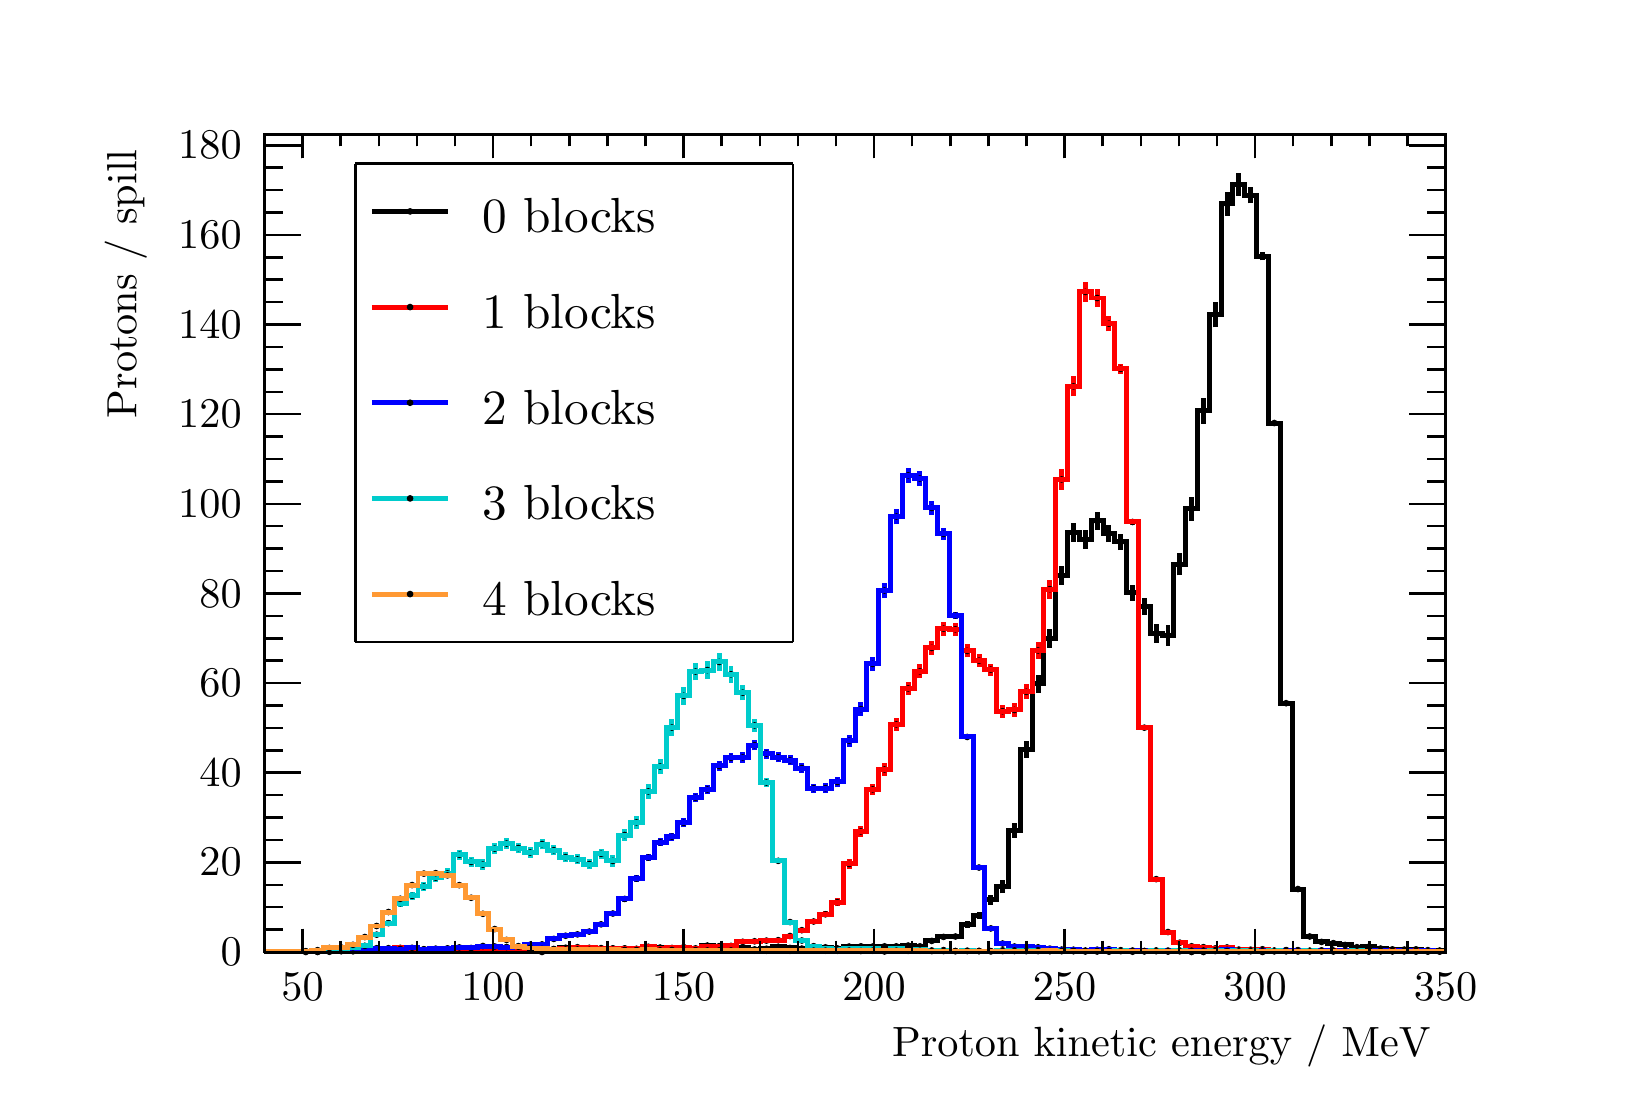
\begin{tikzpicture}
\pgfdeclareplotmark{cross} {
\pgfpathmoveto{\pgfpoint{-0.3\pgfplotmarksize}{\pgfplotmarksize}}
\pgfpathlineto{\pgfpoint{+0.3\pgfplotmarksize}{\pgfplotmarksize}}
\pgfpathlineto{\pgfpoint{+0.3\pgfplotmarksize}{0.3\pgfplotmarksize}}
\pgfpathlineto{\pgfpoint{+1\pgfplotmarksize}{0.3\pgfplotmarksize}}
\pgfpathlineto{\pgfpoint{+1\pgfplotmarksize}{-0.3\pgfplotmarksize}}
\pgfpathlineto{\pgfpoint{+0.3\pgfplotmarksize}{-0.3\pgfplotmarksize}}
\pgfpathlineto{\pgfpoint{+0.3\pgfplotmarksize}{-1.\pgfplotmarksize}}
\pgfpathlineto{\pgfpoint{-0.3\pgfplotmarksize}{-1.\pgfplotmarksize}}
\pgfpathlineto{\pgfpoint{-0.3\pgfplotmarksize}{-0.3\pgfplotmarksize}}
\pgfpathlineto{\pgfpoint{-1.\pgfplotmarksize}{-0.3\pgfplotmarksize}}
\pgfpathlineto{\pgfpoint{-1.\pgfplotmarksize}{0.3\pgfplotmarksize}}
\pgfpathlineto{\pgfpoint{-0.3\pgfplotmarksize}{0.3\pgfplotmarksize}}
\pgfpathclose
\pgfusepathqstroke
}
\pgfdeclareplotmark{cross*} {
\pgfpathmoveto{\pgfpoint{-0.3\pgfplotmarksize}{\pgfplotmarksize}}
\pgfpathlineto{\pgfpoint{+0.3\pgfplotmarksize}{\pgfplotmarksize}}
\pgfpathlineto{\pgfpoint{+0.3\pgfplotmarksize}{0.3\pgfplotmarksize}}
\pgfpathlineto{\pgfpoint{+1\pgfplotmarksize}{0.3\pgfplotmarksize}}
\pgfpathlineto{\pgfpoint{+1\pgfplotmarksize}{-0.3\pgfplotmarksize}}
\pgfpathlineto{\pgfpoint{+0.3\pgfplotmarksize}{-0.3\pgfplotmarksize}}
\pgfpathlineto{\pgfpoint{+0.3\pgfplotmarksize}{-1.\pgfplotmarksize}}
\pgfpathlineto{\pgfpoint{-0.3\pgfplotmarksize}{-1.\pgfplotmarksize}}
\pgfpathlineto{\pgfpoint{-0.3\pgfplotmarksize}{-0.3\pgfplotmarksize}}
\pgfpathlineto{\pgfpoint{-1.\pgfplotmarksize}{-0.3\pgfplotmarksize}}
\pgfpathlineto{\pgfpoint{-1.\pgfplotmarksize}{0.3\pgfplotmarksize}}
\pgfpathlineto{\pgfpoint{-0.3\pgfplotmarksize}{0.3\pgfplotmarksize}}
\pgfpathclose
\pgfusepathqfillstroke
}
\pgfdeclareplotmark{newstar} {
\pgfpathmoveto{\pgfqpoint{0pt}{\pgfplotmarksize}}
\pgfpathlineto{\pgfqpointpolar{44}{0.5\pgfplotmarksize}}
\pgfpathlineto{\pgfqpointpolar{18}{\pgfplotmarksize}}
\pgfpathlineto{\pgfqpointpolar{-20}{0.5\pgfplotmarksize}}
\pgfpathlineto{\pgfqpointpolar{-54}{\pgfplotmarksize}}
\pgfpathlineto{\pgfqpointpolar{-90}{0.5\pgfplotmarksize}}
\pgfpathlineto{\pgfqpointpolar{234}{\pgfplotmarksize}}
\pgfpathlineto{\pgfqpointpolar{198}{0.5\pgfplotmarksize}}
\pgfpathlineto{\pgfqpointpolar{162}{\pgfplotmarksize}}
\pgfpathlineto{\pgfqpointpolar{134}{0.5\pgfplotmarksize}}
\pgfpathclose
\pgfusepathqstroke
}
\pgfdeclareplotmark{newstar*} {
\pgfpathmoveto{\pgfqpoint{0pt}{\pgfplotmarksize}}
\pgfpathlineto{\pgfqpointpolar{44}{0.5\pgfplotmarksize}}
\pgfpathlineto{\pgfqpointpolar{18}{\pgfplotmarksize}}
\pgfpathlineto{\pgfqpointpolar{-20}{0.5\pgfplotmarksize}}
\pgfpathlineto{\pgfqpointpolar{-54}{\pgfplotmarksize}}
\pgfpathlineto{\pgfqpointpolar{-90}{0.5\pgfplotmarksize}}
\pgfpathlineto{\pgfqpointpolar{234}{\pgfplotmarksize}}
\pgfpathlineto{\pgfqpointpolar{198}{0.5\pgfplotmarksize}}
\pgfpathlineto{\pgfqpointpolar{162}{\pgfplotmarksize}}
\pgfpathlineto{\pgfqpointpolar{134}{0.5\pgfplotmarksize}}
\pgfpathclose
\pgfusepathqfillstroke
}
\definecolor{c}{rgb}{1,1,1};
\draw [color=c, fill=c] (0,0) rectangle (20,13.4957);
\draw [color=c, fill=c] (3,1.75444) rectangle (18,12.1461);
\definecolor{c}{rgb}{0,0,0};
\draw [c,line width=0.9] (3,1.75444) -- (3,12.1461) -- (18,12.1461) -- (18,1.75444) -- (3,1.75444);
\definecolor{c}{rgb}{1,1,1};
\draw [color=c, fill=c] (3,1.75444) rectangle (18,12.1461);
\definecolor{c}{rgb}{0,0,0};
\draw [c,line width=0.9] (3,1.75444) -- (3,12.1461) -- (18,12.1461) -- (18,1.75444) -- (3,1.75444);
\draw [c,line width=0.9] (3,1.764) -- (3.15,1.764) -- (3.15,1.764) -- (3.3,1.764) -- (3.3,1.764) -- (3.45,1.764) -- (3.45,1.764) -- (3.6,1.764) -- (3.6,1.764) -- (3.75,1.764) -- (3.75,1.764) -- (3.9,1.764) -- (3.9,1.764) -- (4.05,1.764) --
 (4.05,1.764) -- (4.2,1.764) -- (4.2,1.764) -- (4.35,1.764) -- (4.35,1.764) -- (4.5,1.764) -- (4.5,1.764) -- (4.65,1.764) -- (4.65,1.764) -- (4.8,1.764) -- (4.8,1.764) -- (4.95,1.764) -- (4.95,1.764) -- (5.1,1.764) -- (5.1,1.764) -- (5.25,1.764) --
 (5.25,1.764) -- (5.4,1.764) -- (5.4,1.764) -- (5.55,1.764) -- (5.55,1.764) -- (5.7,1.764) -- (5.7,1.764) -- (5.85,1.764) -- (5.85,1.764) -- (6,1.764) -- (6,1.764) -- (6.15,1.764) -- (6.15,1.764) -- (6.3,1.764) -- (6.3,1.764) -- (6.45,1.764) --
 (6.45,1.764) -- (6.6,1.764) -- (6.6,1.764) -- (6.75,1.764) -- (6.75,1.764) -- (6.9,1.764) -- (6.9,1.764) -- (7.05,1.764) -- (7.05,1.764) -- (7.2,1.764) -- (7.2,1.764) -- (7.35,1.764) -- (7.35,1.764) -- (7.5,1.764) -- (7.5,1.764) -- (7.65,1.764) --
 (7.65,1.764) -- (7.8,1.764) -- (7.8,1.764) -- (7.95,1.764) -- (7.95,1.764) -- (8.1,1.764) -- (8.1,1.764) -- (8.25,1.764) -- (8.25,1.764) -- (8.4,1.764) -- (8.4,1.764) -- (8.55,1.764) -- (8.55,1.764) -- (8.7,1.764) -- (8.7,1.764) -- (8.85,1.764) --
 (8.85,1.764) -- (9,1.764) -- (9,1.764) -- (9.15,1.764) -- (9.15,1.764) -- (9.3,1.764) -- (9.3,1.764) -- (9.45,1.764) -- (9.45,1.764) -- (9.6,1.764) -- (9.6,1.764) -- (9.75,1.764) -- (9.75,1.764) -- (9.9,1.764) -- (9.9,1.764) -- (10.05,1.764) --
 (10.05,1.764) -- (10.2,1.764) -- (10.2,1.764) -- (10.35,1.764) -- (10.35,1.764) -- (10.5,1.764) -- (10.5,1.764) -- (10.65,1.764) -- (10.65,1.764) -- (10.8,1.764) -- (10.8,1.764) -- (10.95,1.764) -- (10.95,1.764) -- (11.1,1.764) -- (11.1,1.764) --
 (11.25,1.764) -- (11.25,1.764) -- (11.4,1.764) -- (11.4,1.764) -- (11.55,1.764) -- (11.55,1.764) -- (11.7,1.764) -- (11.7,1.764) -- (11.85,1.764) -- (11.85,1.764) -- (12,1.764) -- (12,1.764) -- (12.15,1.764) -- (12.15,1.764) -- (12.3,1.764) --
 (12.3,1.764) -- (12.45,1.764) -- (12.45,1.764) -- (12.6,1.764) -- (12.6,1.764) -- (12.75,1.764) -- (12.75,1.764) -- (12.9,1.764) -- (12.9,1.764) -- (13.05,1.764) -- (13.05,1.764) -- (13.2,1.764) -- (13.2,1.764) -- (13.35,1.764) -- (13.35,1.764) --
 (13.5,1.764) -- (13.5,1.764) -- (13.65,1.764) -- (13.65,1.764) -- (13.8,1.764) -- (13.8,1.764) -- (13.95,1.764) -- (13.95,1.764) -- (14.1,1.764) -- (14.1,1.764) -- (14.25,1.764) -- (14.25,1.764) -- (14.4,1.764) -- (14.4,1.764) -- (14.55,1.764) --
 (14.55,1.764) -- (14.7,1.764) -- (14.7,1.764) -- (14.85,1.764) -- (14.85,1.764) -- (15,1.764) -- (15,1.764) -- (15.15,1.764) -- (15.15,1.764) -- (15.3,1.764) -- (15.3,1.764) -- (15.45,1.764) -- (15.45,1.764) -- (15.6,1.764) -- (15.6,1.764) --
 (15.75,1.764) -- (15.75,1.764) -- (15.9,1.764) -- (15.9,1.764) -- (16.05,1.764) -- (16.05,1.764) -- (16.2,1.764) -- (16.2,1.764) -- (16.35,1.764) -- (16.35,1.764) -- (16.5,1.764) -- (16.5,1.764) -- (16.65,1.764) -- (16.65,1.764) -- (16.8,1.764) --
 (16.8,1.764) -- (16.95,1.764) -- (16.95,1.764) -- (17.1,1.764) -- (17.1,1.764) -- (17.25,1.764) -- (17.25,1.764) -- (17.4,1.764) -- (17.4,1.764) -- (17.55,1.764) -- (17.55,1.764) -- (17.7,1.764) -- (17.7,1.764) -- (17.85,1.764) -- (17.85,1.764) --
 (18,1.764);
\draw [c,line width=0.9] (3,1.75444) -- (18,1.75444);
\draw [c,line width=0.9] (3.48387,2.05809) -- (3.48387,1.75444);
\draw [c,line width=0.9] (3.96774,1.90627) -- (3.96774,1.75444);
\draw [c,line width=0.9] (4.45161,1.90627) -- (4.45161,1.75444);
\draw [c,line width=0.9] (4.93548,1.90627) -- (4.93548,1.75444);
\draw [c,line width=0.9] (5.41935,1.90627) -- (5.41935,1.75444);
\draw [c,line width=0.9] (5.90323,2.05809) -- (5.90323,1.75444);
\draw [c,line width=0.9] (6.3871,1.90627) -- (6.3871,1.75444);
\draw [c,line width=0.9] (6.87097,1.90627) -- (6.87097,1.75444);
\draw [c,line width=0.9] (7.35484,1.90627) -- (7.35484,1.75444);
\draw [c,line width=0.9] (7.83871,1.90627) -- (7.83871,1.75444);
\draw [c,line width=0.9] (8.32258,2.05809) -- (8.32258,1.75444);
\draw [c,line width=0.9] (8.80645,1.90627) -- (8.80645,1.75444);
\draw [c,line width=0.9] (9.29032,1.90627) -- (9.29032,1.75444);
\draw [c,line width=0.9] (9.77419,1.90627) -- (9.77419,1.75444);
\draw [c,line width=0.9] (10.2581,1.90627) -- (10.2581,1.75444);
\draw [c,line width=0.9] (10.7419,2.05809) -- (10.7419,1.75444);
\draw [c,line width=0.9] (11.2258,1.90627) -- (11.2258,1.75444);
\draw [c,line width=0.9] (11.7097,1.90627) -- (11.7097,1.75444);
\draw [c,line width=0.9] (12.1935,1.90627) -- (12.1935,1.75444);
\draw [c,line width=0.9] (12.6774,1.90627) -- (12.6774,1.75444);
\draw [c,line width=0.9] (13.1613,2.05809) -- (13.1613,1.75444);
\draw [c,line width=0.9] (13.6452,1.90627) -- (13.6452,1.75444);
\draw [c,line width=0.9] (14.129,1.90627) -- (14.129,1.75444);
\draw [c,line width=0.9] (14.6129,1.90627) -- (14.6129,1.75444);
\draw [c,line width=0.9] (15.0968,1.90627) -- (15.0968,1.75444);
\draw [c,line width=0.9] (15.5806,2.05809) -- (15.5806,1.75444);
\draw [c,line width=0.9] (16.0645,1.90627) -- (16.0645,1.75444);
\draw [c,line width=0.9] (16.5484,1.90627) -- (16.5484,1.75444);
\draw [c,line width=0.9] (17.0323,1.90627) -- (17.0323,1.75444);
\draw [c,line width=0.9] (17.5161,1.90627) -- (17.5161,1.75444);
\draw [c,line width=0.9] (18,2.05809) -- (18,1.75444);
\draw [c,line width=0.9] (3.48387,2.05809) -- (3.48387,1.75444);
\draw [c,line width=0.9] (18,2.05809) -- (18,1.75444);
\draw [anchor=base] (3.48387,1.14713) node[scale=1.52731, color=c, rotate=0]{50};
\draw [anchor=base] (5.90323,1.14713) node[scale=1.52731, color=c, rotate=0]{100};
\draw [anchor=base] (8.32258,1.14713) node[scale=1.52731, color=c, rotate=0]{150};
\draw [anchor=base] (10.7419,1.14713) node[scale=1.52731, color=c, rotate=0]{200};
\draw [anchor=base] (13.1613,1.14713) node[scale=1.52731, color=c, rotate=0]{250};
\draw [anchor=base] (15.5806,1.14713) node[scale=1.52731, color=c, rotate=0]{300};
\draw [anchor=base] (18,1.14713) node[scale=1.52731, color=c, rotate=0]{350};
\draw [anchor= east] (18,0.566819) node[scale=1.52731, color=c, rotate=0]{ Proton kinetic energy / MeV};
\draw [c,line width=0.9] (3,12.1461) -- (18,12.1461);
\draw [c,line width=0.9] (3.48387,11.8425) -- (3.48387,12.1461);
\draw [c,line width=0.9] (3.96774,11.9943) -- (3.96774,12.1461);
\draw [c,line width=0.9] (4.45161,11.9943) -- (4.45161,12.1461);
\draw [c,line width=0.9] (4.93548,11.9943) -- (4.93548,12.1461);
\draw [c,line width=0.9] (5.41935,11.9943) -- (5.41935,12.1461);
\draw [c,line width=0.9] (5.90323,11.8425) -- (5.90323,12.1461);
\draw [c,line width=0.9] (6.3871,11.9943) -- (6.3871,12.1461);
\draw [c,line width=0.9] (6.87097,11.9943) -- (6.87097,12.1461);
\draw [c,line width=0.9] (7.35484,11.9943) -- (7.35484,12.1461);
\draw [c,line width=0.9] (7.83871,11.9943) -- (7.83871,12.1461);
\draw [c,line width=0.9] (8.32258,11.8425) -- (8.32258,12.1461);
\draw [c,line width=0.9] (8.80645,11.9943) -- (8.80645,12.1461);
\draw [c,line width=0.9] (9.29032,11.9943) -- (9.29032,12.1461);
\draw [c,line width=0.9] (9.77419,11.9943) -- (9.77419,12.1461);
\draw [c,line width=0.9] (10.2581,11.9943) -- (10.2581,12.1461);
\draw [c,line width=0.9] (10.7419,11.8425) -- (10.7419,12.1461);
\draw [c,line width=0.9] (11.2258,11.9943) -- (11.2258,12.1461);
\draw [c,line width=0.9] (11.7097,11.9943) -- (11.7097,12.1461);
\draw [c,line width=0.9] (12.1935,11.9943) -- (12.1935,12.1461);
\draw [c,line width=0.9] (12.6774,11.9943) -- (12.6774,12.1461);
\draw [c,line width=0.9] (13.1613,11.8425) -- (13.1613,12.1461);
\draw [c,line width=0.9] (13.6452,11.9943) -- (13.6452,12.1461);
\draw [c,line width=0.9] (14.129,11.9943) -- (14.129,12.1461);
\draw [c,line width=0.9] (14.6129,11.9943) -- (14.6129,12.1461);
\draw [c,line width=0.9] (15.0968,11.9943) -- (15.0968,12.1461);
\draw [c,line width=0.9] (15.5806,11.8425) -- (15.5806,12.1461);
\draw [c,line width=0.9] (16.0645,11.9943) -- (16.0645,12.1461);
\draw [c,line width=0.9] (16.5484,11.9943) -- (16.5484,12.1461);
\draw [c,line width=0.9] (17.0323,11.9943) -- (17.0323,12.1461);
\draw [c,line width=0.9] (17.5161,11.9943) -- (17.5161,12.1461);
\draw [c,line width=0.9] (18,11.8425) -- (18,12.1461);
\draw [c,line width=0.9] (3.48387,11.8425) -- (3.48387,12.1461);
\draw [c,line width=0.9] (18,11.8425) -- (18,12.1461);
\draw [c,line width=0.9] (3,1.75444) -- (3,12.1461);
\draw [c,line width=0.9] (3.462,1.764) -- (3,1.764);
\draw [c,line width=0.9] (3.231,2.04858) -- (3,2.04858);
\draw [c,line width=0.9] (3.231,2.33317) -- (3,2.33317);
\draw [c,line width=0.9] (3.231,2.61775) -- (3,2.61775);
\draw [c,line width=0.9] (3.462,2.90234) -- (3,2.90234);
\draw [c,line width=0.9] (3.231,3.18692) -- (3,3.18692);
\draw [c,line width=0.9] (3.231,3.4715) -- (3,3.4715);
\draw [c,line width=0.9] (3.231,3.75609) -- (3,3.75609);
\draw [c,line width=0.9] (3.462,4.04067) -- (3,4.04067);
\draw [c,line width=0.9] (3.231,4.32526) -- (3,4.32526);
\draw [c,line width=0.9] (3.231,4.60984) -- (3,4.60984);
\draw [c,line width=0.9] (3.231,4.89442) -- (3,4.89442);
\draw [c,line width=0.9] (3.462,5.17901) -- (3,5.17901);
\draw [c,line width=0.9] (3.231,5.46359) -- (3,5.46359);
\draw [c,line width=0.9] (3.231,5.74818) -- (3,5.74818);
\draw [c,line width=0.9] (3.231,6.03276) -- (3,6.03276);
\draw [c,line width=0.9] (3.462,6.31734) -- (3,6.31734);
\draw [c,line width=0.9] (3.231,6.60193) -- (3,6.60193);
\draw [c,line width=0.9] (3.231,6.88651) -- (3,6.88651);
\draw [c,line width=0.9] (3.231,7.1711) -- (3,7.1711);
\draw [c,line width=0.9] (3.462,7.45568) -- (3,7.45568);
\draw [c,line width=0.9] (3.231,7.74026) -- (3,7.74026);
\draw [c,line width=0.9] (3.231,8.02485) -- (3,8.02485);
\draw [c,line width=0.9] (3.231,8.30943) -- (3,8.30943);
\draw [c,line width=0.9] (3.462,8.59402) -- (3,8.59402);
\draw [c,line width=0.9] (3.231,8.8786) -- (3,8.8786);
\draw [c,line width=0.9] (3.231,9.16319) -- (3,9.16319);
\draw [c,line width=0.9] (3.231,9.44777) -- (3,9.44777);
\draw [c,line width=0.9] (3.462,9.73235) -- (3,9.73235);
\draw [c,line width=0.9] (3.231,10.0169) -- (3,10.0169);
\draw [c,line width=0.9] (3.231,10.3015) -- (3,10.3015);
\draw [c,line width=0.9] (3.231,10.5861) -- (3,10.5861);
\draw [c,line width=0.9] (3.462,10.8707) -- (3,10.8707);
\draw [c,line width=0.9] (3.231,11.1553) -- (3,11.1553);
\draw [c,line width=0.9] (3.231,11.4399) -- (3,11.4399);
\draw [c,line width=0.9] (3.231,11.7244) -- (3,11.7244);
\draw [c,line width=0.9] (3.462,12.009) -- (3,12.009);
\draw [c,line width=0.9] (3.462,1.764) -- (3,1.764);
\draw [c,line width=0.9] (3.462,12.009) -- (3,12.009);
\draw [anchor= east] (2.9,1.764) node[scale=1.52731, color=c, rotate=0]{0};
\draw [anchor= east] (2.9,2.90234) node[scale=1.52731, color=c, rotate=0]{20};
\draw [anchor= east] (2.9,4.04067) node[scale=1.52731, color=c, rotate=0]{40};
\draw [anchor= east] (2.9,5.17901) node[scale=1.52731, color=c, rotate=0]{60};
\draw [anchor= east] (2.9,6.31734) node[scale=1.52731, color=c, rotate=0]{80};
\draw [anchor= east] (2.9,7.45568) node[scale=1.52731, color=c, rotate=0]{100};
\draw [anchor= east] (2.9,8.59402) node[scale=1.52731, color=c, rotate=0]{120};
\draw [anchor= east] (2.9,9.73235) node[scale=1.52731, color=c, rotate=0]{140};
\draw [anchor= east] (2.9,10.8707) node[scale=1.52731, color=c, rotate=0]{160};
\draw [anchor= east] (2.9,12.009) node[scale=1.52731, color=c, rotate=0]{180};
\draw [anchor= east] (1.24,12.1461) node[scale=1.52731, color=c, rotate=90]{Protons / spill};
\draw [c,line width=0.9] (18,1.75444) -- (18,12.1461);
\draw [c,line width=0.9] (17.538,1.764) -- (18,1.764);
\draw [c,line width=0.9] (17.769,2.04858) -- (18,2.04858);
\draw [c,line width=0.9] (17.769,2.33317) -- (18,2.33317);
\draw [c,line width=0.9] (17.769,2.61775) -- (18,2.61775);
\draw [c,line width=0.9] (17.538,2.90234) -- (18,2.90234);
\draw [c,line width=0.9] (17.769,3.18692) -- (18,3.18692);
\draw [c,line width=0.9] (17.769,3.4715) -- (18,3.4715);
\draw [c,line width=0.9] (17.769,3.75609) -- (18,3.75609);
\draw [c,line width=0.9] (17.538,4.04067) -- (18,4.04067);
\draw [c,line width=0.9] (17.769,4.32526) -- (18,4.32526);
\draw [c,line width=0.9] (17.769,4.60984) -- (18,4.60984);
\draw [c,line width=0.9] (17.769,4.89442) -- (18,4.89442);
\draw [c,line width=0.9] (17.538,5.17901) -- (18,5.17901);
\draw [c,line width=0.9] (17.769,5.46359) -- (18,5.46359);
\draw [c,line width=0.9] (17.769,5.74818) -- (18,5.74818);
\draw [c,line width=0.9] (17.769,6.03276) -- (18,6.03276);
\draw [c,line width=0.9] (17.538,6.31734) -- (18,6.31734);
\draw [c,line width=0.9] (17.769,6.60193) -- (18,6.60193);
\draw [c,line width=0.9] (17.769,6.88651) -- (18,6.88651);
\draw [c,line width=0.9] (17.769,7.1711) -- (18,7.1711);
\draw [c,line width=0.9] (17.538,7.45568) -- (18,7.45568);
\draw [c,line width=0.9] (17.769,7.74026) -- (18,7.74026);
\draw [c,line width=0.9] (17.769,8.02485) -- (18,8.02485);
\draw [c,line width=0.9] (17.769,8.30943) -- (18,8.30943);
\draw [c,line width=0.9] (17.538,8.59402) -- (18,8.59402);
\draw [c,line width=0.9] (17.769,8.8786) -- (18,8.8786);
\draw [c,line width=0.9] (17.769,9.16319) -- (18,9.16319);
\draw [c,line width=0.9] (17.769,9.44777) -- (18,9.44777);
\draw [c,line width=0.9] (17.538,9.73235) -- (18,9.73235);
\draw [c,line width=0.9] (17.769,10.0169) -- (18,10.0169);
\draw [c,line width=0.9] (17.769,10.3015) -- (18,10.3015);
\draw [c,line width=0.9] (17.769,10.5861) -- (18,10.5861);
\draw [c,line width=0.9] (17.538,10.8707) -- (18,10.8707);
\draw [c,line width=0.9] (17.769,11.1553) -- (18,11.1553);
\draw [c,line width=0.9] (17.769,11.4399) -- (18,11.4399);
\draw [c,line width=0.9] (17.769,11.7244) -- (18,11.7244);
\draw [c,line width=0.9] (17.538,12.009) -- (18,12.009);
\draw [c,line width=0.9] (17.538,1.764) -- (18,1.764);
\draw [c,line width=0.9] (17.538,12.009) -- (18,12.009);
\draw [c,line width=1.8] (6.525,1.75444) -- (6.525,1.764);
\draw [c,line width=1.8] (6.525,1.764) -- (6.525,1.77356);
\foreach \P in {(6.525,1.764)}{\draw[mark options={color=c,fill=c},mark size=2.402402pt,mark=*,mark size=1pt] plot coordinates {\P};}
\draw [c,line width=1.8] (6.675,1.78862) -- (6.675,1.79976);
\draw [c,line width=1.8] (6.675,1.79976) -- (6.675,1.81089);
\foreach \P in {(6.675,1.79976)}{\draw[mark options={color=c,fill=c},mark size=2.402402pt,mark=*,mark size=1pt] plot coordinates {\P};}
\draw [c,line width=1.8] (6.825,1.80879) -- (6.825,1.81764);
\draw [c,line width=1.8] (6.825,1.81764) -- (6.825,1.82649);
\foreach \P in {(6.825,1.81764)}{\draw[mark options={color=c,fill=c},mark size=2.402402pt,mark=*,mark size=1pt] plot coordinates {\P};}
\draw [c,line width=1.8] (6.975,1.78289) -- (6.975,1.7921);
\draw [c,line width=1.8] (6.975,1.7921) -- (6.975,1.80131);
\foreach \P in {(6.975,1.7921)}{\draw[mark options={color=c,fill=c},mark size=2.402402pt,mark=*,mark size=1pt] plot coordinates {\P};}
\draw [c,line width=1.8] (7.125,1.78836) -- (7.125,1.7972);
\draw [c,line width=1.8] (7.125,1.7972) -- (7.125,1.80605);
\foreach \P in {(7.125,1.7972)}{\draw[mark options={color=c,fill=c},mark size=2.402402pt,mark=*,mark size=1pt] plot coordinates {\P};}
\draw [c,line width=1.8] (7.275,1.78578) -- (7.275,1.7972);
\draw [c,line width=1.8] (7.275,1.7972) -- (7.275,1.80863);
\foreach \P in {(7.275,1.7972)}{\draw[mark options={color=c,fill=c},mark size=2.402402pt,mark=*,mark size=1pt] plot coordinates {\P};}
\draw [c,line width=1.8] (7.425,1.79976) -- (7.425,1.80998);
\draw [c,line width=1.8] (7.425,1.80998) -- (7.425,1.82019);
\foreach \P in {(7.425,1.80998)}{\draw[mark options={color=c,fill=c},mark size=2.402402pt,mark=*,mark size=1pt] plot coordinates {\P};}
\draw [c,line width=1.8] (7.575,1.7972) -- (7.575,1.80742);
\draw [c,line width=1.8] (7.575,1.80742) -- (7.575,1.81764);
\foreach \P in {(7.575,1.80742)}{\draw[mark options={color=c,fill=c},mark size=2.402402pt,mark=*,mark size=1pt] plot coordinates {\P};}
\draw [c,line width=1.8] (7.725,1.79178) -- (7.725,1.80231);
\draw [c,line width=1.8] (7.725,1.80231) -- (7.725,1.81284);
\foreach \P in {(7.725,1.80231)}{\draw[mark options={color=c,fill=c},mark size=2.402402pt,mark=*,mark size=1pt] plot coordinates {\P};}
\draw [c,line width=1.8] (7.875,1.79289) -- (7.875,1.80487);
\draw [c,line width=1.8] (7.875,1.80487) -- (7.875,1.81685);
\foreach \P in {(7.875,1.80487)}{\draw[mark options={color=c,fill=c},mark size=2.402402pt,mark=*,mark size=1pt] plot coordinates {\P};}
\draw [c,line width=1.8] (8.025,1.80966) -- (8.025,1.82019);
\draw [c,line width=1.8] (8.025,1.82019) -- (8.025,1.83072);
\foreach \P in {(8.025,1.82019)}{\draw[mark options={color=c,fill=c},mark size=2.402402pt,mark=*,mark size=1pt] plot coordinates {\P};}
\draw [c,line width=1.8] (8.175,1.79517) -- (8.175,1.80742);
\draw [c,line width=1.8] (8.175,1.80742) -- (8.175,1.81967);
\foreach \P in {(8.175,1.80742)}{\draw[mark options={color=c,fill=c},mark size=2.402402pt,mark=*,mark size=1pt] plot coordinates {\P};}
\draw [c,line width=1.8] (8.325,1.81477) -- (8.325,1.8253);
\draw [c,line width=1.8] (8.325,1.8253) -- (8.325,1.83583);
\foreach \P in {(8.325,1.8253)}{\draw[mark options={color=c,fill=c},mark size=2.402402pt,mark=*,mark size=1pt] plot coordinates {\P};}
\draw [c,line width=1.8] (8.475,1.78321) -- (8.475,1.7972);
\draw [c,line width=1.8] (8.475,1.7972) -- (8.475,1.8112);
\foreach \P in {(8.475,1.7972)}{\draw[mark options={color=c,fill=c},mark size=2.402402pt,mark=*,mark size=1pt] plot coordinates {\P};}
\draw [c,line width=1.8] (8.625,1.83403) -- (8.625,1.84573);
\draw [c,line width=1.8] (8.625,1.84573) -- (8.625,1.85744);
\foreach \P in {(8.625,1.84573)}{\draw[mark options={color=c,fill=c},mark size=2.402402pt,mark=*,mark size=1pt] plot coordinates {\P};}
\draw [c,line width=1.8] (8.775,1.81023) -- (8.775,1.82275);
\draw [c,line width=1.8] (8.775,1.82275) -- (8.775,1.83526);
\foreach \P in {(8.775,1.82275)}{\draw[mark options={color=c,fill=c},mark size=2.402402pt,mark=*,mark size=1pt] plot coordinates {\P};}
\draw [c,line width=1.8] (8.925,1.79373) -- (8.925,1.80487);
\draw [c,line width=1.8] (8.925,1.80487) -- (8.925,1.816);
\foreach \P in {(8.925,1.80487)}{\draw[mark options={color=c,fill=c},mark size=2.402402pt,mark=*,mark size=1pt] plot coordinates {\P};}
\draw [c,line width=1.8] (9.075,1.81354) -- (9.075,1.82275);
\draw [c,line width=1.8] (9.075,1.82275) -- (9.075,1.83196);
\foreach \P in {(9.075,1.82275)}{\draw[mark options={color=c,fill=c},mark size=2.402402pt,mark=*,mark size=1pt] plot coordinates {\P};}
\draw [c,line width=1.8] (9.225,1.78607) -- (9.225,1.7972);
\draw [c,line width=1.8] (9.225,1.7972) -- (9.225,1.80834);
\foreach \P in {(9.225,1.7972)}{\draw[mark options={color=c,fill=c},mark size=2.402402pt,mark=*,mark size=1pt] plot coordinates {\P};}
\draw [c,line width=1.8] (9.375,1.79209) -- (9.375,1.80487);
\draw [c,line width=1.8] (9.375,1.80487) -- (9.375,1.81764);
\foreach \P in {(9.375,1.80487)}{\draw[mark options={color=c,fill=c},mark size=2.402402pt,mark=*,mark size=1pt] plot coordinates {\P};}
\draw [c,line width=1.8] (9.525,1.81643) -- (9.525,1.82785);
\draw [c,line width=1.8] (9.525,1.82785) -- (9.525,1.83928);
\foreach \P in {(9.525,1.82785)}{\draw[mark options={color=c,fill=c},mark size=2.402402pt,mark=*,mark size=1pt] plot coordinates {\P};}
\draw [c,line width=1.8] (9.675,1.80231) -- (9.675,1.81508);
\draw [c,line width=1.8] (9.675,1.81508) -- (9.675,1.82786);
\foreach \P in {(9.675,1.81508)}{\draw[mark options={color=c,fill=c},mark size=2.402402pt,mark=*,mark size=1pt] plot coordinates {\P};}
\draw [c,line width=1.8] (9.825,1.79491) -- (9.825,1.80742);
\draw [c,line width=1.8] (9.825,1.80742) -- (9.825,1.81994);
\foreach \P in {(9.825,1.80742)}{\draw[mark options={color=c,fill=c},mark size=2.402402pt,mark=*,mark size=1pt] plot coordinates {\P};}
\draw [c,line width=1.8] (9.975,1.8187) -- (9.975,1.83041);
\draw [c,line width=1.8] (9.975,1.83041) -- (9.975,1.84212);
\foreach \P in {(9.975,1.83041)}{\draw[mark options={color=c,fill=c},mark size=2.402402pt,mark=*,mark size=1pt] plot coordinates {\P};}
\draw [c,line width=1.8] (10.125,1.81023) -- (10.125,1.82275);
\draw [c,line width=1.8] (10.125,1.82275) -- (10.125,1.83526);
\foreach \P in {(10.125,1.82275)}{\draw[mark options={color=c,fill=c},mark size=2.402402pt,mark=*,mark size=1pt] plot coordinates {\P};}
\draw [c,line width=1.8] (10.275,1.79646) -- (10.275,1.80998);
\draw [c,line width=1.8] (10.275,1.80998) -- (10.275,1.82349);
\foreach \P in {(10.275,1.80998)}{\draw[mark options={color=c,fill=c},mark size=2.402402pt,mark=*,mark size=1pt] plot coordinates {\P};}
\draw [c,line width=1.8] (10.425,1.81994) -- (10.425,1.83296);
\draw [c,line width=1.8] (10.425,1.83296) -- (10.425,1.84599);
\foreach \P in {(10.425,1.83296)}{\draw[mark options={color=c,fill=c},mark size=2.402402pt,mark=*,mark size=1pt] plot coordinates {\P};}
\draw [c,line width=1.8] (10.575,1.82107) -- (10.575,1.83552);
\draw [c,line width=1.8] (10.575,1.83552) -- (10.575,1.84997);
\foreach \P in {(10.575,1.83552)}{\draw[mark options={color=c,fill=c},mark size=2.402402pt,mark=*,mark size=1pt] plot coordinates {\P};}
\draw [c,line width=1.8] (10.725,1.82098) -- (10.725,1.83296);
\draw [c,line width=1.8] (10.725,1.83296) -- (10.725,1.84494);
\foreach \P in {(10.725,1.83296)}{\draw[mark options={color=c,fill=c},mark size=2.402402pt,mark=*,mark size=1pt] plot coordinates {\P};}
\draw [c,line width=1.8] (10.875,1.81936) -- (10.875,1.83552);
\draw [c,line width=1.8] (10.875,1.83552) -- (10.875,1.85167);
\foreach \P in {(10.875,1.83552)}{\draw[mark options={color=c,fill=c},mark size=2.402402pt,mark=*,mark size=1pt] plot coordinates {\P};}
\draw [c,line width=1.8] (11.025,1.82249) -- (11.025,1.83552);
\draw [c,line width=1.8] (11.025,1.83552) -- (11.025,1.84854);
\foreach \P in {(11.025,1.83552)}{\draw[mark options={color=c,fill=c},mark size=2.402402pt,mark=*,mark size=1pt] plot coordinates {\P};}
\draw [c,line width=1.8] (11.175,1.82938) -- (11.175,1.84573);
\draw [c,line width=1.8] (11.175,1.84573) -- (11.175,1.86209);
\foreach \P in {(11.175,1.84573)}{\draw[mark options={color=c,fill=c},mark size=2.402402pt,mark=*,mark size=1pt] plot coordinates {\P};}
\draw [c,line width=1.8] (11.325,1.81296) -- (11.325,1.83552);
\draw [c,line width=1.8] (11.325,1.83552) -- (11.325,1.85808);
\foreach \P in {(11.325,1.83552)}{\draw[mark options={color=c,fill=c},mark size=2.402402pt,mark=*,mark size=1pt] plot coordinates {\P};}
\draw [c,line width=1.8] (11.475,1.88192) -- (11.475,1.90448);
\draw [c,line width=1.8] (11.475,1.90448) -- (11.475,1.92704);
\foreach \P in {(11.475,1.90448)}{\draw[mark options={color=c,fill=c},mark size=2.402402pt,mark=*,mark size=1pt] plot coordinates {\P};}
\draw [c,line width=1.8] (11.625,1.92667) -- (11.625,1.95557);
\draw [c,line width=1.8] (11.625,1.95557) -- (11.625,1.98447);
\foreach \P in {(11.625,1.95557)}{\draw[mark options={color=c,fill=c},mark size=2.402402pt,mark=*,mark size=1pt] plot coordinates {\P};}
\draw [c,line width=1.8] (11.775,1.92593) -- (11.775,1.96068);
\draw [c,line width=1.8] (11.775,1.96068) -- (11.775,1.99542);
\foreach \P in {(11.775,1.96068)}{\draw[mark options={color=c,fill=c},mark size=2.402402pt,mark=*,mark size=1pt] plot coordinates {\P};}
\draw [c,line width=1.8] (11.925,2.07131) -- (11.925,2.11138);
\draw [c,line width=1.8] (11.925,2.11138) -- (11.925,2.15144);
\foreach \P in {(11.925,2.11138)}{\draw[mark options={color=c,fill=c},mark size=2.402402pt,mark=*,mark size=1pt] plot coordinates {\P};}
\draw [c,line width=1.8] (12.075,2.1797) -- (12.075,2.22632);
\draw [c,line width=1.8] (12.075,2.22632) -- (12.075,2.27293);
\foreach \P in {(12.075,2.22632)}{\draw[mark options={color=c,fill=c},mark size=2.402402pt,mark=*,mark size=1pt] plot coordinates {\P};}
\draw [c,line width=1.8] (12.225,2.36501) -- (12.225,2.4281);
\draw [c,line width=1.8] (12.225,2.4281) -- (12.225,2.49119);
\foreach \P in {(12.225,2.4281)}{\draw[mark options={color=c,fill=c},mark size=2.402402pt,mark=*,mark size=1pt] plot coordinates {\P};}
\draw [c,line width=1.8] (12.375,2.50943) -- (12.375,2.59157);
\draw [c,line width=1.8] (12.375,2.59157) -- (12.375,2.67371);
\foreach \P in {(12.375,2.59157)}{\draw[mark options={color=c,fill=c},mark size=2.402402pt,mark=*,mark size=1pt] plot coordinates {\P};}
\draw [c,line width=1.8] (12.525,3.2117) -- (12.525,3.30676);
\draw [c,line width=1.8] (12.525,3.30676) -- (12.525,3.40183);
\foreach \P in {(12.525,3.30676)}{\draw[mark options={color=c,fill=c},mark size=2.402402pt,mark=*,mark size=1pt] plot coordinates {\P};}
\draw [c,line width=1.8] (12.675,4.2329) -- (12.675,4.33612);
\draw [c,line width=1.8] (12.675,4.33612) -- (12.675,4.43935);
\foreach \P in {(12.675,4.33612)}{\draw[mark options={color=c,fill=c},mark size=2.402402pt,mark=*,mark size=1pt] plot coordinates {\P};}
\draw [c,line width=1.8] (12.825,5.05822) -- (12.825,5.17136);
\draw [c,line width=1.8] (12.825,5.17136) -- (12.825,5.28451);
\foreach \P in {(12.825,5.17136)}{\draw[mark options={color=c,fill=c},mark size=2.402402pt,mark=*,mark size=1pt] plot coordinates {\P};}
\draw [c,line width=1.8] (12.975,5.62743) -- (12.975,5.74607);
\draw [c,line width=1.8] (12.975,5.74607) -- (12.975,5.8647);
\foreach \P in {(12.975,5.74607)}{\draw[mark options={color=c,fill=c},mark size=2.402402pt,mark=*,mark size=1pt] plot coordinates {\P};}
\draw [c,line width=1.8] (13.125,6.42458) -- (13.125,6.54299);
\draw [c,line width=1.8] (13.125,6.54299) -- (13.125,6.66141);
\foreach \P in {(13.125,6.54299)}{\draw[mark options={color=c,fill=c},mark size=2.402402pt,mark=*,mark size=1pt] plot coordinates {\P};}
\draw [c,line width=1.8] (13.275,6.97517) -- (13.275,7.09471);
\draw [c,line width=1.8] (13.275,7.09471) -- (13.275,7.21425);
\foreach \P in {(13.275,7.09471)}{\draw[mark options={color=c,fill=c},mark size=2.402402pt,mark=*,mark size=1pt] plot coordinates {\P};}
\draw [c,line width=1.8] (13.425,6.88463) -- (13.425,7.00531);
\draw [c,line width=1.8] (13.425,7.00531) -- (13.425,7.12599);
\foreach \P in {(13.425,7.00531)}{\draw[mark options={color=c,fill=c},mark size=2.402402pt,mark=*,mark size=1pt] plot coordinates {\P};}
\draw [c,line width=1.8] (13.575,7.12466) -- (13.575,7.23775);
\draw [c,line width=1.8] (13.575,7.23775) -- (13.575,7.35083);
\foreach \P in {(13.575,7.23775)}{\draw[mark options={color=c,fill=c},mark size=2.402402pt,mark=*,mark size=1pt] plot coordinates {\P};}
\draw [c,line width=1.8] (13.725,6.96898) -- (13.725,7.07938);
\draw [c,line width=1.8] (13.725,7.07938) -- (13.725,7.18978);
\foreach \P in {(13.725,7.07938)}{\draw[mark options={color=c,fill=c},mark size=2.402402pt,mark=*,mark size=1pt] plot coordinates {\P};}
\draw [c,line width=1.8] (13.875,6.86691) -- (13.875,6.9721);
\draw [c,line width=1.8] (13.875,6.9721) -- (13.875,7.0773);
\foreach \P in {(13.875,6.9721)}{\draw[mark options={color=c,fill=c},mark size=2.402402pt,mark=*,mark size=1pt] plot coordinates {\P};}
\draw [c,line width=1.8] (14.025,6.22607) -- (14.025,6.32843);
\draw [c,line width=1.8] (14.025,6.32843) -- (14.025,6.4308);
\foreach \P in {(14.025,6.32843)}{\draw[mark options={color=c,fill=c},mark size=2.402402pt,mark=*,mark size=1pt] plot coordinates {\P};}
\draw [c,line width=1.8] (14.175,6.04448) -- (14.175,6.15219);
\draw [c,line width=1.8] (14.175,6.15219) -- (14.175,6.2599);
\foreach \P in {(14.175,6.15219)}{\draw[mark options={color=c,fill=c},mark size=2.402402pt,mark=*,mark size=1pt] plot coordinates {\P};}
\draw [c,line width=1.8] (14.325,5.68981) -- (14.325,5.80737);
\draw [c,line width=1.8] (14.325,5.80737) -- (14.325,5.92493);
\foreach \P in {(14.325,5.80737)}{\draw[mark options={color=c,fill=c},mark size=2.402402pt,mark=*,mark size=1pt] plot coordinates {\P};}
\draw [c,line width=1.8] (14.475,5.65582) -- (14.475,5.78438);
\draw [c,line width=1.8] (14.475,5.78438) -- (14.475,5.91294);
\foreach \P in {(14.475,5.78438)}{\draw[mark options={color=c,fill=c},mark size=2.402402pt,mark=*,mark size=1pt] plot coordinates {\P};}
\draw [c,line width=1.8] (14.625,6.54781) -- (14.625,6.68858);
\draw [c,line width=1.8] (14.625,6.68858) -- (14.625,6.82935);
\foreach \P in {(14.625,6.68858)}{\draw[mark options={color=c,fill=c},mark size=2.402402pt,mark=*,mark size=1pt] plot coordinates {\P};}
\draw [c,line width=1.8] (14.775,7.23695) -- (14.775,7.391);
\draw [c,line width=1.8] (14.775,7.391) -- (14.775,7.54505);
\foreach \P in {(14.775,7.391)}{\draw[mark options={color=c,fill=c},mark size=2.402402pt,mark=*,mark size=1pt] plot coordinates {\P};}
\draw [c,line width=1.8] (14.925,8.47236) -- (14.925,8.63492);
\draw [c,line width=1.8] (14.925,8.63492) -- (14.925,8.79748);
\foreach \P in {(14.925,8.63492)}{\draw[mark options={color=c,fill=c},mark size=2.402402pt,mark=*,mark size=1pt] plot coordinates {\P};}
\draw [c,line width=1.8] (15.075,9.69782) -- (15.075,9.8584);
\draw [c,line width=1.8] (15.075,9.8584) -- (15.075,10.019);
\foreach \P in {(15.075,9.8584)}{\draw[mark options={color=c,fill=c},mark size=2.402402pt,mark=*,mark size=1pt] plot coordinates {\P};}
\draw [c,line width=1.8] (15.225,11.1112) -- (15.225,11.2658);
\draw [c,line width=1.8] (15.225,11.2658) -- (15.225,11.4204);
\foreach \P in {(15.225,11.2658)}{\draw[mark options={color=c,fill=c},mark size=2.402402pt,mark=*,mark size=1pt] plot coordinates {\P};}
\draw [c,line width=1.8] (15.375,11.3702) -- (15.375,11.511);
\draw [c,line width=1.8] (15.375,11.511) -- (15.375,11.6517);
\foreach \P in {(15.375,11.511)}{\draw[mark options={color=c,fill=c},mark size=2.402402pt,mark=*,mark size=1pt] plot coordinates {\P};}
\draw [c,line width=1.8] (15.525,11.2696) -- (15.525,11.3731);
\draw [c,line width=1.8] (15.525,11.3731) -- (15.525,11.4765);
\foreach \P in {(15.525,11.3731)}{\draw[mark options={color=c,fill=c},mark size=2.402402pt,mark=*,mark size=1pt] plot coordinates {\P};}
\draw [c,line width=1.8] (15.675,10.5474) -- (15.675,10.6017);
\draw [c,line width=1.8] (15.675,10.6017) -- (15.675,10.6559);
\foreach \P in {(15.675,10.6017)}{\draw[mark options={color=c,fill=c},mark size=2.402402pt,mark=*,mark size=1pt] plot coordinates {\P};}
\draw [c,line width=1.8] (15.825,8.45825) -- (15.825,8.48166);
\draw [c,line width=1.8] (15.825,8.48166) -- (15.825,8.50507);
\foreach \P in {(15.825,8.48166)}{\draw[mark options={color=c,fill=c},mark size=2.402402pt,mark=*,mark size=1pt] plot coordinates {\P};}
\draw [c,line width=1.8] (15.975,4.905) -- (15.975,4.9236);
\draw [c,line width=1.8] (15.975,4.9236) -- (15.975,4.9422);
\foreach \P in {(15.975,4.9236)}{\draw[mark options={color=c,fill=c},mark size=2.402402pt,mark=*,mark size=1pt] plot coordinates {\P};}
\draw [c,line width=1.8] (16.125,2.54578) -- (16.125,2.56348);
\draw [c,line width=1.8] (16.125,2.56348) -- (16.125,2.58117);
\foreach \P in {(16.125,2.56348)}{\draw[mark options={color=c,fill=c},mark size=2.402402pt,mark=*,mark size=1pt] plot coordinates {\P};}
\draw [c,line width=1.8] (16.275,1.94514) -- (16.275,1.96068);
\draw [c,line width=1.8] (16.275,1.96068) -- (16.275,1.97621);
\foreach \P in {(16.275,1.96068)}{\draw[mark options={color=c,fill=c},mark size=2.402402pt,mark=*,mark size=1pt] plot coordinates {\P};}
\draw [c,line width=1.8] (16.425,1.87894) -- (16.425,1.89171);
\draw [c,line width=1.8] (16.425,1.89171) -- (16.425,1.90448);
\foreach \P in {(16.425,1.89171)}{\draw[mark options={color=c,fill=c},mark size=2.402402pt,mark=*,mark size=1pt] plot coordinates {\P};}
\draw [c,line width=1.8] (16.575,1.86311) -- (16.575,1.87639);
\draw [c,line width=1.8] (16.575,1.87639) -- (16.575,1.88966);
\foreach \P in {(16.575,1.87639)}{\draw[mark options={color=c,fill=c},mark size=2.402402pt,mark=*,mark size=1pt] plot coordinates {\P};}
\draw [c,line width=1.8] (16.725,1.84287) -- (16.725,1.8534);
\draw [c,line width=1.8] (16.725,1.8534) -- (16.725,1.86393);
\foreach \P in {(16.725,1.8534)}{\draw[mark options={color=c,fill=c},mark size=2.402402pt,mark=*,mark size=1pt] plot coordinates {\P};}
\draw [c,line width=1.8] (16.875,1.81541) -- (16.875,1.8253);
\draw [c,line width=1.8] (16.875,1.8253) -- (16.875,1.83519);
\foreach \P in {(16.875,1.8253)}{\draw[mark options={color=c,fill=c},mark size=2.402402pt,mark=*,mark size=1pt] plot coordinates {\P};}
\draw [c,line width=1.8] (17.025,1.82275) -- (17.025,1.83041);
\draw [c,line width=1.8] (17.025,1.83041) -- (17.025,1.83807);
\foreach \P in {(17.025,1.83041)}{\draw[mark options={color=c,fill=c},mark size=2.402402pt,mark=*,mark size=1pt] plot coordinates {\P};}
\draw [c,line width=1.8] (17.175,1.79786) -- (17.175,1.80742);
\draw [c,line width=1.8] (17.175,1.80742) -- (17.175,1.81698);
\foreach \P in {(17.175,1.80742)}{\draw[mark options={color=c,fill=c},mark size=2.402402pt,mark=*,mark size=1pt] plot coordinates {\P};}
\draw [c,line width=1.8] (17.325,1.78836) -- (17.325,1.7972);
\draw [c,line width=1.8] (17.325,1.7972) -- (17.325,1.80605);
\foreach \P in {(17.325,1.7972)}{\draw[mark options={color=c,fill=c},mark size=2.402402pt,mark=*,mark size=1pt] plot coordinates {\P};}
\draw [c,line width=1.8] (17.475,1.79104) -- (17.475,1.79465);
\draw [c,line width=1.8] (17.475,1.79465) -- (17.475,1.79826);
\foreach \P in {(17.475,1.79465)}{\draw[mark options={color=c,fill=c},mark size=2.402402pt,mark=*,mark size=1pt] plot coordinates {\P};}
\foreach \P in {(17.625,1.7972)}{\draw[mark options={color=c,fill=c},mark size=2.402402pt,mark=*,mark size=1pt] plot coordinates {\P};}
\foreach \P in {(17.775,1.78699)}{\draw[mark options={color=c,fill=c},mark size=2.402402pt,mark=*,mark size=1pt] plot coordinates {\P};}
\foreach \P in {(17.925,1.78188)}{\draw[mark options={color=c,fill=c},mark size=2.402402pt,mark=*,mark size=1pt] plot coordinates {\P};}
\draw [c,line width=1.8] (3,1.764) -- (3.15,1.764) -- (3.15,1.764) -- (3.3,1.764) -- (3.3,1.764) -- (3.45,1.764) -- (3.45,1.764) -- (3.6,1.764) -- (3.6,1.764) -- (3.75,1.764) -- (3.75,1.764) -- (3.9,1.764) -- (3.9,1.764) -- (4.05,1.764) --
 (4.05,1.764) -- (4.2,1.764) -- (4.2,1.764) -- (4.35,1.764) -- (4.35,1.764) -- (4.5,1.764) -- (4.5,1.764) -- (4.65,1.764) -- (4.65,1.764) -- (4.8,1.764) -- (4.8,1.764) -- (4.95,1.764) -- (4.95,1.764) -- (5.1,1.764) -- (5.1,1.764) -- (5.25,1.764) --
 (5.25,1.764) -- (5.4,1.764) -- (5.4,1.764) -- (5.55,1.764) -- (5.55,1.764) -- (5.7,1.764) -- (5.7,1.764) -- (5.85,1.764) -- (5.85,1.764) -- (6,1.764) -- (6,1.764) -- (6.15,1.764) -- (6.15,1.764) -- (6.3,1.764) -- (6.3,1.764) -- (6.45,1.764) --
 (6.45,1.764) -- (6.6,1.764) -- (6.6,1.79976) -- (6.75,1.79976) -- (6.75,1.81764) -- (6.9,1.81764) -- (6.9,1.7921) -- (7.05,1.7921) -- (7.05,1.7972) -- (7.2,1.7972) -- (7.2,1.7972) -- (7.35,1.7972) -- (7.35,1.80998) -- (7.5,1.80998) -- (7.5,1.80742)
 -- (7.65,1.80742) -- (7.65,1.80231) -- (7.8,1.80231) -- (7.8,1.80487) -- (7.95,1.80487) -- (7.95,1.82019) -- (8.1,1.82019) -- (8.1,1.80742) -- (8.25,1.80742) -- (8.25,1.8253) -- (8.4,1.8253) -- (8.4,1.7972) -- (8.55,1.7972) -- (8.55,1.84573) --
 (8.7,1.84573) -- (8.7,1.82275) -- (8.85,1.82275) -- (8.85,1.80487) -- (9,1.80487) -- (9,1.82275) -- (9.15,1.82275) -- (9.15,1.7972) -- (9.3,1.7972) -- (9.3,1.80487) -- (9.45,1.80487) -- (9.45,1.82785) -- (9.6,1.82785) -- (9.6,1.81508) --
 (9.75,1.81508) -- (9.75,1.80742) -- (9.9,1.80742) -- (9.9,1.83041) -- (10.05,1.83041) -- (10.05,1.82275) -- (10.2,1.82275) -- (10.2,1.80998) -- (10.35,1.80998) -- (10.35,1.83296) -- (10.5,1.83296) -- (10.5,1.83552) -- (10.65,1.83552) --
 (10.65,1.83296) -- (10.8,1.83296) -- (10.8,1.83552) -- (10.95,1.83552) -- (10.95,1.83552) -- (11.1,1.83552) -- (11.1,1.84573) -- (11.25,1.84573) -- (11.25,1.83552) -- (11.4,1.83552) -- (11.4,1.90448) -- (11.55,1.90448) -- (11.55,1.95557) --
 (11.7,1.95557) -- (11.7,1.96068) -- (11.85,1.96068) -- (11.85,2.11138) -- (12,2.11138) -- (12,2.22632) -- (12.15,2.22632) -- (12.15,2.4281) -- (12.3,2.4281) -- (12.3,2.59157) -- (12.45,2.59157) -- (12.45,3.30676) -- (12.6,3.30676) -- (12.6,4.33612)
 -- (12.75,4.33612) -- (12.75,5.17136) -- (12.9,5.17136) -- (12.9,5.74607) -- (13.05,5.74607) -- (13.05,6.54299) -- (13.2,6.54299) -- (13.2,7.09471) -- (13.35,7.09471) -- (13.35,7.00531) -- (13.5,7.00531) -- (13.5,7.23775) -- (13.65,7.23775) --
 (13.65,7.07938) -- (13.8,7.07938) -- (13.8,6.9721) -- (13.95,6.9721) -- (13.95,6.32843) -- (14.1,6.32843) -- (14.1,6.15219) -- (14.25,6.15219) -- (14.25,5.80737) -- (14.4,5.80737) -- (14.4,5.78438) -- (14.55,5.78438) -- (14.55,6.68858) --
 (14.7,6.68858) -- (14.7,7.391) -- (14.85,7.391) -- (14.85,8.63492) -- (15,8.63492) -- (15,9.8584) -- (15.15,9.8584) -- (15.15,11.2658) -- (15.3,11.2658) -- (15.3,11.511) -- (15.45,11.511) -- (15.45,11.3731) -- (15.6,11.3731) -- (15.6,10.6017) --
 (15.75,10.6017) -- (15.75,8.48166) -- (15.9,8.48166) -- (15.9,4.9236) -- (16.05,4.9236) -- (16.05,2.56348) -- (16.2,2.56348) -- (16.2,1.96068) -- (16.35,1.96068) -- (16.35,1.89171) -- (16.5,1.89171) -- (16.5,1.87639) -- (16.65,1.87639) --
 (16.65,1.8534) -- (16.8,1.8534) -- (16.8,1.8253) -- (16.95,1.8253) -- (16.95,1.83041) -- (17.1,1.83041) -- (17.1,1.80742) -- (17.25,1.80742) -- (17.25,1.7972) -- (17.4,1.7972) -- (17.4,1.79465) -- (17.55,1.79465) -- (17.55,1.7972) -- (17.7,1.7972)
 -- (17.7,1.78699) -- (17.85,1.78699) -- (17.85,1.78188) -- (18,1.78188);
\definecolor{c}{rgb}{1,0,0};
\draw [c,line width=1.8] (3.675,1.76232) -- (3.675,1.764);
\draw [c,line width=1.8] (3.675,1.764) -- (3.675,1.76568);
\definecolor{c}{rgb}{0,0,0};
\foreach \P in {(3.675,1.764)}{\draw[mark options={color=c,fill=c},mark size=2.402402pt,mark=*,mark size=1pt] plot coordinates {\P};}
\definecolor{c}{rgb}{1,0,0};
\draw [c,line width=1.8] (3.825,1.76692) -- (3.825,1.77103);
\draw [c,line width=1.8] (3.825,1.77103) -- (3.825,1.77513);
\definecolor{c}{rgb}{0,0,0};
\foreach \P in {(3.825,1.77103)}{\draw[mark options={color=c,fill=c},mark size=2.402402pt,mark=*,mark size=1pt] plot coordinates {\P};}
\definecolor{c}{rgb}{1,0,0};
\draw [c,line width=1.8] (3.975,1.77194) -- (3.975,1.77704);
\draw [c,line width=1.8] (3.975,1.77704) -- (3.975,1.78214);
\definecolor{c}{rgb}{0,0,0};
\foreach \P in {(3.975,1.77704)}{\draw[mark options={color=c,fill=c},mark size=2.402402pt,mark=*,mark size=1pt] plot coordinates {\P};}
\definecolor{c}{rgb}{1,0,0};
\draw [c,line width=1.8] (4.125,1.78028) -- (4.125,1.78818);
\draw [c,line width=1.8] (4.125,1.78818) -- (4.125,1.79609);
\definecolor{c}{rgb}{0,0,0};
\foreach \P in {(4.125,1.78818)}{\draw[mark options={color=c,fill=c},mark size=2.402402pt,mark=*,mark size=1pt] plot coordinates {\P};}
\definecolor{c}{rgb}{1,0,0};
\draw [c,line width=1.8] (4.275,1.79219) -- (4.275,1.80221);
\draw [c,line width=1.8] (4.275,1.80221) -- (4.275,1.81223);
\definecolor{c}{rgb}{0,0,0};
\foreach \P in {(4.275,1.80221)}{\draw[mark options={color=c,fill=c},mark size=2.402402pt,mark=*,mark size=1pt] plot coordinates {\P};}
\definecolor{c}{rgb}{1,0,0};
\draw [c,line width=1.8] (4.425,1.79972) -- (4.425,1.8082);
\draw [c,line width=1.8] (4.425,1.8082) -- (4.425,1.81667);
\definecolor{c}{rgb}{0,0,0};
\foreach \P in {(4.425,1.8082)}{\draw[mark options={color=c,fill=c},mark size=2.402402pt,mark=*,mark size=1pt] plot coordinates {\P};}
\definecolor{c}{rgb}{1,0,0};
\draw [c,line width=1.8] (4.575,1.80112) -- (4.575,1.81192);
\draw [c,line width=1.8] (4.575,1.81192) -- (4.575,1.82272);
\definecolor{c}{rgb}{0,0,0};
\foreach \P in {(4.575,1.81192)}{\draw[mark options={color=c,fill=c},mark size=2.402402pt,mark=*,mark size=1pt] plot coordinates {\P};}
\definecolor{c}{rgb}{1,0,0};
\draw [c,line width=1.8] (4.725,1.80718) -- (4.725,1.81639);
\draw [c,line width=1.8] (4.725,1.81639) -- (4.725,1.8256);
\definecolor{c}{rgb}{0,0,0};
\foreach \P in {(4.725,1.81639)}{\draw[mark options={color=c,fill=c},mark size=2.402402pt,mark=*,mark size=1pt] plot coordinates {\P};}
\definecolor{c}{rgb}{1,0,0};
\draw [c,line width=1.8] (4.875,1.79102) -- (4.875,1.799);
\draw [c,line width=1.8] (4.875,1.799) -- (4.875,1.80697);
\definecolor{c}{rgb}{0,0,0};
\foreach \P in {(4.875,1.799)}{\draw[mark options={color=c,fill=c},mark size=2.402402pt,mark=*,mark size=1pt] plot coordinates {\P};}
\definecolor{c}{rgb}{1,0,0};
\draw [c,line width=1.8] (5.025,1.79041) -- (5.025,1.79879);
\draw [c,line width=1.8] (5.025,1.79879) -- (5.025,1.80716);
\definecolor{c}{rgb}{0,0,0};
\foreach \P in {(5.025,1.79879)}{\draw[mark options={color=c,fill=c},mark size=2.402402pt,mark=*,mark size=1pt] plot coordinates {\P};}
\definecolor{c}{rgb}{1,0,0};
\draw [c,line width=1.8] (5.175,1.78817) -- (5.175,1.79617);
\draw [c,line width=1.8] (5.175,1.79617) -- (5.175,1.80417);
\definecolor{c}{rgb}{0,0,0};
\foreach \P in {(5.175,1.79617)}{\draw[mark options={color=c,fill=c},mark size=2.402402pt,mark=*,mark size=1pt] plot coordinates {\P};}
\definecolor{c}{rgb}{1,0,0};
\draw [c,line width=1.8] (5.325,1.7993) -- (5.325,1.80841);
\draw [c,line width=1.8] (5.325,1.80841) -- (5.325,1.81753);
\definecolor{c}{rgb}{0,0,0};
\foreach \P in {(5.325,1.80841)}{\draw[mark options={color=c,fill=c},mark size=2.402402pt,mark=*,mark size=1pt] plot coordinates {\P};}
\definecolor{c}{rgb}{1,0,0};
\draw [c,line width=1.8] (5.475,1.78882) -- (5.475,1.79611);
\draw [c,line width=1.8] (5.475,1.79611) -- (5.475,1.80341);
\definecolor{c}{rgb}{0,0,0};
\foreach \P in {(5.475,1.79611)}{\draw[mark options={color=c,fill=c},mark size=2.402402pt,mark=*,mark size=1pt] plot coordinates {\P};}
\definecolor{c}{rgb}{1,0,0};
\draw [c,line width=1.8] (5.625,1.79229) -- (5.625,1.80146);
\draw [c,line width=1.8] (5.625,1.80146) -- (5.625,1.81062);
\definecolor{c}{rgb}{0,0,0};
\foreach \P in {(5.625,1.80146)}{\draw[mark options={color=c,fill=c},mark size=2.402402pt,mark=*,mark size=1pt] plot coordinates {\P};}
\definecolor{c}{rgb}{1,0,0};
\draw [c,line width=1.8] (5.775,1.80037) -- (5.775,1.80879);
\draw [c,line width=1.8] (5.775,1.80879) -- (5.775,1.81721);
\definecolor{c}{rgb}{0,0,0};
\foreach \P in {(5.775,1.80879)}{\draw[mark options={color=c,fill=c},mark size=2.402402pt,mark=*,mark size=1pt] plot coordinates {\P};}
\definecolor{c}{rgb}{1,0,0};
\draw [c,line width=1.8] (5.925,1.79207) -- (5.925,1.80087);
\draw [c,line width=1.8] (5.925,1.80087) -- (5.925,1.80967);
\definecolor{c}{rgb}{0,0,0};
\foreach \P in {(5.925,1.80087)}{\draw[mark options={color=c,fill=c},mark size=2.402402pt,mark=*,mark size=1pt] plot coordinates {\P};}
\definecolor{c}{rgb}{1,0,0};
\draw [c,line width=1.8] (6.075,1.78003) -- (6.075,1.78818);
\draw [c,line width=1.8] (6.075,1.78818) -- (6.075,1.79632);
\definecolor{c}{rgb}{0,0,0};
\foreach \P in {(6.075,1.78818)}{\draw[mark options={color=c,fill=c},mark size=2.402402pt,mark=*,mark size=1pt] plot coordinates {\P};}
\definecolor{c}{rgb}{1,0,0};
\draw [c,line width=1.8] (6.225,1.79725) -- (6.225,1.80814);
\draw [c,line width=1.8] (6.225,1.80814) -- (6.225,1.81902);
\definecolor{c}{rgb}{0,0,0};
\foreach \P in {(6.225,1.80814)}{\draw[mark options={color=c,fill=c},mark size=2.402402pt,mark=*,mark size=1pt] plot coordinates {\P};}
\definecolor{c}{rgb}{1,0,0};
\draw [c,line width=1.8] (6.375,1.8093) -- (6.375,1.81971);
\draw [c,line width=1.8] (6.375,1.81971) -- (6.375,1.83011);
\definecolor{c}{rgb}{0,0,0};
\foreach \P in {(6.375,1.81971)}{\draw[mark options={color=c,fill=c},mark size=2.402402pt,mark=*,mark size=1pt] plot coordinates {\P};}
\definecolor{c}{rgb}{1,0,0};
\draw [c,line width=1.8] (6.525,1.80777) -- (6.525,1.81583);
\draw [c,line width=1.8] (6.525,1.81583) -- (6.525,1.82389);
\definecolor{c}{rgb}{0,0,0};
\foreach \P in {(6.525,1.81583)}{\draw[mark options={color=c,fill=c},mark size=2.402402pt,mark=*,mark size=1pt] plot coordinates {\P};}
\definecolor{c}{rgb}{1,0,0};
\draw [c,line width=1.8] (6.675,1.79017) -- (6.675,1.79888);
\draw [c,line width=1.8] (6.675,1.79888) -- (6.675,1.8076);
\definecolor{c}{rgb}{0,0,0};
\foreach \P in {(6.675,1.79888)}{\draw[mark options={color=c,fill=c},mark size=2.402402pt,mark=*,mark size=1pt] plot coordinates {\P};}
\definecolor{c}{rgb}{1,0,0};
\draw [c,line width=1.8] (6.825,1.79816) -- (6.825,1.80951);
\draw [c,line width=1.8] (6.825,1.80951) -- (6.825,1.82085);
\definecolor{c}{rgb}{0,0,0};
\foreach \P in {(6.825,1.80951)}{\draw[mark options={color=c,fill=c},mark size=2.402402pt,mark=*,mark size=1pt] plot coordinates {\P};}
\definecolor{c}{rgb}{1,0,0};
\draw [c,line width=1.8] (6.975,1.81454) -- (6.975,1.8243);
\draw [c,line width=1.8] (6.975,1.8243) -- (6.975,1.83406);
\definecolor{c}{rgb}{0,0,0};
\foreach \P in {(6.975,1.8243)}{\draw[mark options={color=c,fill=c},mark size=2.402402pt,mark=*,mark size=1pt] plot coordinates {\P};}
\definecolor{c}{rgb}{1,0,0};
\draw [c,line width=1.8] (7.125,1.80666) -- (7.125,1.81694);
\draw [c,line width=1.8] (7.125,1.81694) -- (7.125,1.82723);
\definecolor{c}{rgb}{0,0,0};
\foreach \P in {(7.125,1.81694)}{\draw[mark options={color=c,fill=c},mark size=2.402402pt,mark=*,mark size=1pt] plot coordinates {\P};}
\definecolor{c}{rgb}{1,0,0};
\draw [c,line width=1.8] (7.275,1.80382) -- (7.275,1.8131);
\draw [c,line width=1.8] (7.275,1.8131) -- (7.275,1.82237);
\definecolor{c}{rgb}{0,0,0};
\foreach \P in {(7.275,1.8131)}{\draw[mark options={color=c,fill=c},mark size=2.402402pt,mark=*,mark size=1pt] plot coordinates {\P};}
\definecolor{c}{rgb}{1,0,0};
\draw [c,line width=1.8] (7.425,1.79882) -- (7.425,1.80809);
\draw [c,line width=1.8] (7.425,1.80809) -- (7.425,1.81735);
\definecolor{c}{rgb}{0,0,0};
\foreach \P in {(7.425,1.80809)}{\draw[mark options={color=c,fill=c},mark size=2.402402pt,mark=*,mark size=1pt] plot coordinates {\P};}
\definecolor{c}{rgb}{1,0,0};
\draw [c,line width=1.8] (7.575,1.80038) -- (7.575,1.80977);
\draw [c,line width=1.8] (7.575,1.80977) -- (7.575,1.81916);
\definecolor{c}{rgb}{0,0,0};
\foreach \P in {(7.575,1.80977)}{\draw[mark options={color=c,fill=c},mark size=2.402402pt,mark=*,mark size=1pt] plot coordinates {\P};}
\definecolor{c}{rgb}{1,0,0};
\draw [c,line width=1.8] (7.725,1.79195) -- (7.725,1.80325);
\draw [c,line width=1.8] (7.725,1.80325) -- (7.725,1.81456);
\definecolor{c}{rgb}{0,0,0};
\foreach \P in {(7.725,1.80325)}{\draw[mark options={color=c,fill=c},mark size=2.402402pt,mark=*,mark size=1pt] plot coordinates {\P};}
\definecolor{c}{rgb}{1,0,0};
\draw [c,line width=1.8] (7.875,1.82118) -- (7.875,1.83017);
\draw [c,line width=1.8] (7.875,1.83017) -- (7.875,1.83916);
\definecolor{c}{rgb}{0,0,0};
\foreach \P in {(7.875,1.83017)}{\draw[mark options={color=c,fill=c},mark size=2.402402pt,mark=*,mark size=1pt] plot coordinates {\P};}
\definecolor{c}{rgb}{1,0,0};
\draw [c,line width=1.8] (8.025,1.79611) -- (8.025,1.8061);
\draw [c,line width=1.8] (8.025,1.8061) -- (8.025,1.81608);
\definecolor{c}{rgb}{0,0,0};
\foreach \P in {(8.025,1.8061)}{\draw[mark options={color=c,fill=c},mark size=2.402402pt,mark=*,mark size=1pt] plot coordinates {\P};}
\definecolor{c}{rgb}{1,0,0};
\draw [c,line width=1.8] (8.175,1.80446) -- (8.175,1.81483);
\draw [c,line width=1.8] (8.175,1.81483) -- (8.175,1.8252);
\definecolor{c}{rgb}{0,0,0};
\foreach \P in {(8.175,1.81483)}{\draw[mark options={color=c,fill=c},mark size=2.402402pt,mark=*,mark size=1pt] plot coordinates {\P};}
\definecolor{c}{rgb}{1,0,0};
\draw [c,line width=1.8] (8.325,1.81126) -- (8.325,1.82017);
\draw [c,line width=1.8] (8.325,1.82017) -- (8.325,1.82907);
\definecolor{c}{rgb}{0,0,0};
\foreach \P in {(8.325,1.82017)}{\draw[mark options={color=c,fill=c},mark size=2.402402pt,mark=*,mark size=1pt] plot coordinates {\P};}
\definecolor{c}{rgb}{1,0,0};
\draw [c,line width=1.8] (8.475,1.79818) -- (8.475,1.81018);
\draw [c,line width=1.8] (8.475,1.81018) -- (8.475,1.82218);
\definecolor{c}{rgb}{0,0,0};
\foreach \P in {(8.475,1.81018)}{\draw[mark options={color=c,fill=c},mark size=2.402402pt,mark=*,mark size=1pt] plot coordinates {\P};}
\definecolor{c}{rgb}{1,0,0};
\draw [c,line width=1.8] (8.625,1.82047) -- (8.625,1.83259);
\draw [c,line width=1.8] (8.625,1.83259) -- (8.625,1.8447);
\definecolor{c}{rgb}{0,0,0};
\foreach \P in {(8.625,1.83259)}{\draw[mark options={color=c,fill=c},mark size=2.402402pt,mark=*,mark size=1pt] plot coordinates {\P};}
\definecolor{c}{rgb}{1,0,0};
\draw [c,line width=1.8] (8.775,1.82535) -- (8.775,1.83805);
\draw [c,line width=1.8] (8.775,1.83805) -- (8.775,1.85076);
\definecolor{c}{rgb}{0,0,0};
\foreach \P in {(8.775,1.83805)}{\draw[mark options={color=c,fill=c},mark size=2.402402pt,mark=*,mark size=1pt] plot coordinates {\P};}
\definecolor{c}{rgb}{1,0,0};
\draw [c,line width=1.8] (8.925,1.82447) -- (8.925,1.84119);
\draw [c,line width=1.8] (8.925,1.84119) -- (8.925,1.85791);
\definecolor{c}{rgb}{0,0,0};
\foreach \P in {(8.925,1.84119)}{\draw[mark options={color=c,fill=c},mark size=2.402402pt,mark=*,mark size=1pt] plot coordinates {\P};}
\definecolor{c}{rgb}{1,0,0};
\draw [c,line width=1.8] (9.075,1.87655) -- (9.075,1.89313);
\draw [c,line width=1.8] (9.075,1.89313) -- (9.075,1.90972);
\definecolor{c}{rgb}{0,0,0};
\foreach \P in {(9.075,1.89313)}{\draw[mark options={color=c,fill=c},mark size=2.402402pt,mark=*,mark size=1pt] plot coordinates {\P};}
\definecolor{c}{rgb}{1,0,0};
\draw [c,line width=1.8] (9.225,1.88377) -- (9.225,1.89968);
\draw [c,line width=1.8] (9.225,1.89968) -- (9.225,1.91559);
\definecolor{c}{rgb}{0,0,0};
\foreach \P in {(9.225,1.89968)}{\draw[mark options={color=c,fill=c},mark size=2.402402pt,mark=*,mark size=1pt] plot coordinates {\P};}
\definecolor{c}{rgb}{1,0,0};
\draw [c,line width=1.8] (9.375,1.88963) -- (9.375,1.90852);
\draw [c,line width=1.8] (9.375,1.90852) -- (9.375,1.92741);
\definecolor{c}{rgb}{0,0,0};
\foreach \P in {(9.375,1.90852)}{\draw[mark options={color=c,fill=c},mark size=2.402402pt,mark=*,mark size=1pt] plot coordinates {\P};}
\definecolor{c}{rgb}{1,0,0};
\draw [c,line width=1.8] (9.525,1.89241) -- (9.525,1.91415);
\draw [c,line width=1.8] (9.525,1.91415) -- (9.525,1.93588);
\definecolor{c}{rgb}{0,0,0};
\foreach \P in {(9.525,1.91415)}{\draw[mark options={color=c,fill=c},mark size=2.402402pt,mark=*,mark size=1pt] plot coordinates {\P};}
\definecolor{c}{rgb}{1,0,0};
\draw [c,line width=1.8] (9.675,1.94181) -- (9.675,1.96653);
\draw [c,line width=1.8] (9.675,1.96653) -- (9.675,1.99125);
\definecolor{c}{rgb}{0,0,0};
\foreach \P in {(9.675,1.96653)}{\draw[mark options={color=c,fill=c},mark size=2.402402pt,mark=*,mark size=1pt] plot coordinates {\P};}
\definecolor{c}{rgb}{1,0,0};
\draw [c,line width=1.8] (9.825,2.01174) -- (9.825,2.04084);
\draw [c,line width=1.8] (9.825,2.04084) -- (9.825,2.06994);
\definecolor{c}{rgb}{0,0,0};
\foreach \P in {(9.825,2.04084)}{\draw[mark options={color=c,fill=c},mark size=2.402402pt,mark=*,mark size=1pt] plot coordinates {\P};}
\definecolor{c}{rgb}{1,0,0};
\draw [c,line width=1.8] (9.975,2.11956) -- (9.975,2.15123);
\draw [c,line width=1.8] (9.975,2.15123) -- (9.975,2.1829);
\definecolor{c}{rgb}{0,0,0};
\foreach \P in {(9.975,2.15123)}{\draw[mark options={color=c,fill=c},mark size=2.402402pt,mark=*,mark size=1pt] plot coordinates {\P};}
\definecolor{c}{rgb}{1,0,0};
\draw [c,line width=1.8] (10.125,2.20273) -- (10.125,2.24266);
\draw [c,line width=1.8] (10.125,2.24266) -- (10.125,2.28259);
\definecolor{c}{rgb}{0,0,0};
\foreach \P in {(10.125,2.24266)}{\draw[mark options={color=c,fill=c},mark size=2.402402pt,mark=*,mark size=1pt] plot coordinates {\P};}
\definecolor{c}{rgb}{1,0,0};
\draw [c,line width=1.8] (10.275,2.34476) -- (10.275,2.39623);
\draw [c,line width=1.8] (10.275,2.39623) -- (10.275,2.44771);
\definecolor{c}{rgb}{0,0,0};
\foreach \P in {(10.275,2.39623)}{\draw[mark options={color=c,fill=c},mark size=2.402402pt,mark=*,mark size=1pt] plot coordinates {\P};}
\definecolor{c}{rgb}{1,0,0};
\draw [c,line width=1.8] (10.425,2.82106) -- (10.425,2.88152);
\draw [c,line width=1.8] (10.425,2.88152) -- (10.425,2.94198);
\definecolor{c}{rgb}{0,0,0};
\foreach \P in {(10.425,2.88152)}{\draw[mark options={color=c,fill=c},mark size=2.402402pt,mark=*,mark size=1pt] plot coordinates {\P};}
\definecolor{c}{rgb}{1,0,0};
\draw [c,line width=1.8] (10.575,3.22955) -- (10.575,3.29513);
\draw [c,line width=1.8] (10.575,3.29513) -- (10.575,3.36072);
\definecolor{c}{rgb}{0,0,0};
\foreach \P in {(10.575,3.29513)}{\draw[mark options={color=c,fill=c},mark size=2.402402pt,mark=*,mark size=1pt] plot coordinates {\P};}
\definecolor{c}{rgb}{1,0,0};
\draw [c,line width=1.8] (10.725,3.75646) -- (10.725,3.82894);
\draw [c,line width=1.8] (10.725,3.82894) -- (10.725,3.90141);
\definecolor{c}{rgb}{0,0,0};
\foreach \P in {(10.725,3.82894)}{\draw[mark options={color=c,fill=c},mark size=2.402402pt,mark=*,mark size=1pt] plot coordinates {\P};}
\definecolor{c}{rgb}{1,0,0};
\draw [c,line width=1.8] (10.875,4.00373) -- (10.875,4.08185);
\draw [c,line width=1.8] (10.875,4.08185) -- (10.875,4.15998);
\definecolor{c}{rgb}{0,0,0};
\foreach \P in {(10.875,4.08185)}{\draw[mark options={color=c,fill=c},mark size=2.402402pt,mark=*,mark size=1pt] plot coordinates {\P};}
\definecolor{c}{rgb}{1,0,0};
\draw [c,line width=1.8] (11.025,4.57168) -- (11.025,4.65424);
\draw [c,line width=1.8] (11.025,4.65424) -- (11.025,4.7368);
\definecolor{c}{rgb}{0,0,0};
\foreach \P in {(11.025,4.65424)}{\draw[mark options={color=c,fill=c},mark size=2.402402pt,mark=*,mark size=1pt] plot coordinates {\P};}
\definecolor{c}{rgb}{1,0,0};
\draw [c,line width=1.8] (11.175,5.02466) -- (11.175,5.11085);
\draw [c,line width=1.8] (11.175,5.11085) -- (11.175,5.19704);
\definecolor{c}{rgb}{0,0,0};
\foreach \P in {(11.175,5.11085)}{\draw[mark options={color=c,fill=c},mark size=2.402402pt,mark=*,mark size=1pt] plot coordinates {\P};}
\definecolor{c}{rgb}{1,0,0};
\draw [c,line width=1.8] (11.325,5.23949) -- (11.325,5.32818);
\draw [c,line width=1.8] (11.325,5.32818) -- (11.325,5.41687);
\definecolor{c}{rgb}{0,0,0};
\foreach \P in {(11.325,5.32818)}{\draw[mark options={color=c,fill=c},mark size=2.402402pt,mark=*,mark size=1pt] plot coordinates {\P};}
\definecolor{c}{rgb}{1,0,0};
\draw [c,line width=1.8] (11.475,5.53683) -- (11.475,5.62566);
\draw [c,line width=1.8] (11.475,5.62566) -- (11.475,5.71449);
\definecolor{c}{rgb}{0,0,0};
\foreach \P in {(11.475,5.62566)}{\draw[mark options={color=c,fill=c},mark size=2.402402pt,mark=*,mark size=1pt] plot coordinates {\P};}
\definecolor{c}{rgb}{1,0,0};
\draw [c,line width=1.8] (11.625,5.78207) -- (11.625,5.86964);
\draw [c,line width=1.8] (11.625,5.86964) -- (11.625,5.9572);
\definecolor{c}{rgb}{0,0,0};
\foreach \P in {(11.625,5.86964)}{\draw[mark options={color=c,fill=c},mark size=2.402402pt,mark=*,mark size=1pt] plot coordinates {\P};}
\definecolor{c}{rgb}{1,0,0};
\draw [c,line width=1.8] (11.775,5.77602) -- (11.775,5.86191);
\draw [c,line width=1.8] (11.775,5.86191) -- (11.775,5.9478);
\definecolor{c}{rgb}{0,0,0};
\foreach \P in {(11.775,5.86191)}{\draw[mark options={color=c,fill=c},mark size=2.402402pt,mark=*,mark size=1pt] plot coordinates {\P};}
\definecolor{c}{rgb}{1,0,0};
\draw [c,line width=1.8] (11.925,5.50461) -- (11.925,5.58766);
\draw [c,line width=1.8] (11.925,5.58766) -- (11.925,5.67071);
\definecolor{c}{rgb}{0,0,0};
\foreach \P in {(11.925,5.58766)}{\draw[mark options={color=c,fill=c},mark size=2.402402pt,mark=*,mark size=1pt] plot coordinates {\P};}
\definecolor{c}{rgb}{1,0,0};
\draw [c,line width=1.8] (12.075,5.38556) -- (12.075,5.46392);
\draw [c,line width=1.8] (12.075,5.46392) -- (12.075,5.54229);
\definecolor{c}{rgb}{0,0,0};
\foreach \P in {(12.075,5.46392)}{\draw[mark options={color=c,fill=c},mark size=2.402402pt,mark=*,mark size=1pt] plot coordinates {\P};}
\definecolor{c}{rgb}{1,0,0};
\draw [c,line width=1.8] (12.225,5.2731) -- (12.225,5.35024);
\draw [c,line width=1.8] (12.225,5.35024) -- (12.225,5.42738);
\definecolor{c}{rgb}{0,0,0};
\foreach \P in {(12.225,5.35024)}{\draw[mark options={color=c,fill=c},mark size=2.402402pt,mark=*,mark size=1pt] plot coordinates {\P};}
\definecolor{c}{rgb}{1,0,0};
\draw [c,line width=1.8] (12.375,4.7413) -- (12.375,4.82168);
\draw [c,line width=1.8] (12.375,4.82168) -- (12.375,4.90206);
\definecolor{c}{rgb}{0,0,0};
\foreach \P in {(12.375,4.82168)}{\draw[mark options={color=c,fill=c},mark size=2.402402pt,mark=*,mark size=1pt] plot coordinates {\P};}
\definecolor{c}{rgb}{1,0,0};
\draw [c,line width=1.8] (12.525,4.75052) -- (12.525,4.8375);
\draw [c,line width=1.8] (12.525,4.8375) -- (12.525,4.92448);
\definecolor{c}{rgb}{0,0,0};
\foreach \P in {(12.525,4.8375)}{\draw[mark options={color=c,fill=c},mark size=2.402402pt,mark=*,mark size=1pt] plot coordinates {\P};}
\definecolor{c}{rgb}{1,0,0};
\draw [c,line width=1.8] (12.675,4.97159) -- (12.675,5.06765);
\draw [c,line width=1.8] (12.675,5.06765) -- (12.675,5.1637);
\definecolor{c}{rgb}{0,0,0};
\foreach \P in {(12.675,5.06765)}{\draw[mark options={color=c,fill=c},mark size=2.402402pt,mark=*,mark size=1pt] plot coordinates {\P};}
\definecolor{c}{rgb}{1,0,0};
\draw [c,line width=1.8] (12.825,5.48383) -- (12.825,5.59325);
\draw [c,line width=1.8] (12.825,5.59325) -- (12.825,5.70267);
\definecolor{c}{rgb}{0,0,0};
\foreach \P in {(12.825,5.59325)}{\draw[mark options={color=c,fill=c},mark size=2.402402pt,mark=*,mark size=1pt] plot coordinates {\P};}
\definecolor{c}{rgb}{1,0,0};
\draw [c,line width=1.8] (12.975,6.25237) -- (12.975,6.37207);
\draw [c,line width=1.8] (12.975,6.37207) -- (12.975,6.49176);
\definecolor{c}{rgb}{0,0,0};
\foreach \P in {(12.975,6.37207)}{\draw[mark options={color=c,fill=c},mark size=2.402402pt,mark=*,mark size=1pt] plot coordinates {\P};}
\definecolor{c}{rgb}{1,0,0};
\draw [c,line width=1.8] (13.125,7.63679) -- (13.125,7.76536);
\draw [c,line width=1.8] (13.125,7.76536) -- (13.125,7.89394);
\definecolor{c}{rgb}{0,0,0};
\foreach \P in {(13.125,7.76536)}{\draw[mark options={color=c,fill=c},mark size=2.402402pt,mark=*,mark size=1pt] plot coordinates {\P};}
\definecolor{c}{rgb}{1,0,0};
\draw [c,line width=1.8] (13.275,8.81964) -- (13.275,8.94725);
\draw [c,line width=1.8] (13.275,8.94725) -- (13.275,9.07486);
\definecolor{c}{rgb}{0,0,0};
\foreach \P in {(13.275,8.94725)}{\draw[mark options={color=c,fill=c},mark size=2.402402pt,mark=*,mark size=1pt] plot coordinates {\P};}
\definecolor{c}{rgb}{1,0,0};
\draw [c,line width=1.8] (13.425,10.0228) -- (13.425,10.1466);
\draw [c,line width=1.8] (13.425,10.1466) -- (13.425,10.2703);
\definecolor{c}{rgb}{0,0,0};
\foreach \P in {(13.425,10.1466)}{\draw[mark options={color=c,fill=c},mark size=2.402402pt,mark=*,mark size=1pt] plot coordinates {\P};}
\definecolor{c}{rgb}{1,0,0};
\draw [c,line width=1.8] (13.575,9.95232) -- (13.575,10.0695);
\draw [c,line width=1.8] (13.575,10.0695) -- (13.575,10.1866);
\definecolor{c}{rgb}{0,0,0};
\foreach \P in {(13.575,10.0695)}{\draw[mark options={color=c,fill=c},mark size=2.402402pt,mark=*,mark size=1pt] plot coordinates {\P};}
\definecolor{c}{rgb}{1,0,0};
\draw [c,line width=1.8] (13.725,9.64712) -- (13.725,9.7433);
\draw [c,line width=1.8] (13.725,9.7433) -- (13.725,9.83947);
\definecolor{c}{rgb}{0,0,0};
\foreach \P in {(13.725,9.7433)}{\draw[mark options={color=c,fill=c},mark size=2.402402pt,mark=*,mark size=1pt] plot coordinates {\P};}
\definecolor{c}{rgb}{1,0,0};
\draw [c,line width=1.8] (13.875,9.10728) -- (13.875,9.1695);
\draw [c,line width=1.8] (13.875,9.1695) -- (13.875,9.23172);
\definecolor{c}{rgb}{0,0,0};
\foreach \P in {(13.875,9.1695)}{\draw[mark options={color=c,fill=c},mark size=2.402402pt,mark=*,mark size=1pt] plot coordinates {\P};}
\definecolor{c}{rgb}{1,0,0};
\draw [c,line width=1.8] (14.025,7.1921) -- (14.025,7.22517);
\draw [c,line width=1.8] (14.025,7.22517) -- (14.025,7.25823);
\definecolor{c}{rgb}{0,0,0};
\foreach \P in {(14.025,7.22517)}{\draw[mark options={color=c,fill=c},mark size=2.402402pt,mark=*,mark size=1pt] plot coordinates {\P};}
\definecolor{c}{rgb}{1,0,0};
\draw [c,line width=1.8] (14.175,4.59444) -- (14.175,4.61287);
\draw [c,line width=1.8] (14.175,4.61287) -- (14.175,4.6313);
\definecolor{c}{rgb}{0,0,0};
\foreach \P in {(14.175,4.61287)}{\draw[mark options={color=c,fill=c},mark size=2.402402pt,mark=*,mark size=1pt] plot coordinates {\P};}
\definecolor{c}{rgb}{1,0,0};
\draw [c,line width=1.8] (14.325,2.67685) -- (14.325,2.68928);
\draw [c,line width=1.8] (14.325,2.68928) -- (14.325,2.70171);
\definecolor{c}{rgb}{0,0,0};
\foreach \P in {(14.325,2.68928)}{\draw[mark options={color=c,fill=c},mark size=2.402402pt,mark=*,mark size=1pt] plot coordinates {\P};}
\definecolor{c}{rgb}{1,0,0};
\draw [c,line width=1.8] (14.475,2.00457) -- (14.475,2.01712);
\draw [c,line width=1.8] (14.475,2.01712) -- (14.475,2.02967);
\definecolor{c}{rgb}{0,0,0};
\foreach \P in {(14.475,2.01712)}{\draw[mark options={color=c,fill=c},mark size=2.402402pt,mark=*,mark size=1pt] plot coordinates {\P};}
\definecolor{c}{rgb}{1,0,0};
\draw [c,line width=1.8] (14.625,1.8728) -- (14.625,1.88207);
\draw [c,line width=1.8] (14.625,1.88207) -- (14.625,1.89134);
\definecolor{c}{rgb}{0,0,0};
\foreach \P in {(14.625,1.88207)}{\draw[mark options={color=c,fill=c},mark size=2.402402pt,mark=*,mark size=1pt] plot coordinates {\P};}
\definecolor{c}{rgb}{1,0,0};
\draw [c,line width=1.8] (14.775,1.82442) -- (14.775,1.83621);
\draw [c,line width=1.8] (14.775,1.83621) -- (14.775,1.848);
\definecolor{c}{rgb}{0,0,0};
\foreach \P in {(14.775,1.83621)}{\draw[mark options={color=c,fill=c},mark size=2.402402pt,mark=*,mark size=1pt] plot coordinates {\P};}
\definecolor{c}{rgb}{1,0,0};
\draw [c,line width=1.8] (14.925,1.8172) -- (14.925,1.8251);
\draw [c,line width=1.8] (14.925,1.8251) -- (14.925,1.83299);
\definecolor{c}{rgb}{0,0,0};
\foreach \P in {(14.925,1.8251)}{\draw[mark options={color=c,fill=c},mark size=2.402402pt,mark=*,mark size=1pt] plot coordinates {\P};}
\definecolor{c}{rgb}{1,0,0};
\draw [c,line width=1.8] (15.075,1.80189) -- (15.075,1.80933);
\draw [c,line width=1.8] (15.075,1.80933) -- (15.075,1.81677);
\definecolor{c}{rgb}{0,0,0};
\foreach \P in {(15.075,1.80933)}{\draw[mark options={color=c,fill=c},mark size=2.402402pt,mark=*,mark size=1pt] plot coordinates {\P};}
\definecolor{c}{rgb}{1,0,0};
\draw [c,line width=1.8] (15.225,1.81396) -- (15.225,1.82166);
\draw [c,line width=1.8] (15.225,1.82166) -- (15.225,1.82937);
\definecolor{c}{rgb}{0,0,0};
\foreach \P in {(15.225,1.82166)}{\draw[mark options={color=c,fill=c},mark size=2.402402pt,mark=*,mark size=1pt] plot coordinates {\P};}
\definecolor{c}{rgb}{1,0,0};
\draw [c,line width=1.8] (15.375,1.78884) -- (15.375,1.79438);
\draw [c,line width=1.8] (15.375,1.79438) -- (15.375,1.79991);
\definecolor{c}{rgb}{0,0,0};
\foreach \P in {(15.375,1.79438)}{\draw[mark options={color=c,fill=c},mark size=2.402402pt,mark=*,mark size=1pt] plot coordinates {\P};}
\definecolor{c}{rgb}{1,0,0};
\draw [c,line width=1.8] (15.525,1.78582) -- (15.525,1.79286);
\draw [c,line width=1.8] (15.525,1.79286) -- (15.525,1.7999);
\definecolor{c}{rgb}{0,0,0};
\foreach \P in {(15.525,1.79286)}{\draw[mark options={color=c,fill=c},mark size=2.402402pt,mark=*,mark size=1pt] plot coordinates {\P};}
\definecolor{c}{rgb}{1,0,0};
\draw [c,line width=1.8] (15.675,1.79193) -- (15.675,1.79845);
\draw [c,line width=1.8] (15.675,1.79845) -- (15.675,1.80497);
\definecolor{c}{rgb}{0,0,0};
\foreach \P in {(15.675,1.79845)}{\draw[mark options={color=c,fill=c},mark size=2.402402pt,mark=*,mark size=1pt] plot coordinates {\P};}
\definecolor{c}{rgb}{1,0,0};
\draw [c,line width=1.8] (15.825,1.77202) -- (15.825,1.77785);
\draw [c,line width=1.8] (15.825,1.77785) -- (15.825,1.78367);
\definecolor{c}{rgb}{0,0,0};
\foreach \P in {(15.825,1.77785)}{\draw[mark options={color=c,fill=c},mark size=2.402402pt,mark=*,mark size=1pt] plot coordinates {\P};}
\definecolor{c}{rgb}{1,0,0};
\draw [c,line width=1.8] (15.975,1.77993) -- (15.975,1.78573);
\draw [c,line width=1.8] (15.975,1.78573) -- (15.975,1.79154);
\definecolor{c}{rgb}{0,0,0};
\foreach \P in {(15.975,1.78573)}{\draw[mark options={color=c,fill=c},mark size=2.402402pt,mark=*,mark size=1pt] plot coordinates {\P};}
\definecolor{c}{rgb}{1,0,0};
\draw [c,line width=1.8] (16.125,1.78132) -- (16.125,1.78755);
\draw [c,line width=1.8] (16.125,1.78755) -- (16.125,1.79378);
\definecolor{c}{rgb}{0,0,0};
\foreach \P in {(16.125,1.78755)}{\draw[mark options={color=c,fill=c},mark size=2.402402pt,mark=*,mark size=1pt] plot coordinates {\P};}
\definecolor{c}{rgb}{1,0,0};
\draw [c,line width=1.8] (16.275,1.77306) -- (16.275,1.77942);
\draw [c,line width=1.8] (16.275,1.77942) -- (16.275,1.78578);
\definecolor{c}{rgb}{0,0,0};
\foreach \P in {(16.275,1.77942)}{\draw[mark options={color=c,fill=c},mark size=2.402402pt,mark=*,mark size=1pt] plot coordinates {\P};}
\definecolor{c}{rgb}{1,0,0};
\draw [c,line width=1.8] (16.425,1.77832) -- (16.425,1.78319);
\draw [c,line width=1.8] (16.425,1.78319) -- (16.425,1.78806);
\definecolor{c}{rgb}{0,0,0};
\foreach \P in {(16.425,1.78319)}{\draw[mark options={color=c,fill=c},mark size=2.402402pt,mark=*,mark size=1pt] plot coordinates {\P};}
\definecolor{c}{rgb}{1,0,0};
\draw [c,line width=1.8] (16.575,1.77858) -- (16.575,1.7824);
\draw [c,line width=1.8] (16.575,1.7824) -- (16.575,1.78622);
\definecolor{c}{rgb}{0,0,0};
\foreach \P in {(16.575,1.7824)}{\draw[mark options={color=c,fill=c},mark size=2.402402pt,mark=*,mark size=1pt] plot coordinates {\P};}
\definecolor{c}{rgb}{1,0,0};
\draw [c,line width=1.8] (16.725,1.77909) -- (16.725,1.78554);
\draw [c,line width=1.8] (16.725,1.78554) -- (16.725,1.792);
\definecolor{c}{rgb}{0,0,0};
\foreach \P in {(16.725,1.78554)}{\draw[mark options={color=c,fill=c},mark size=2.402402pt,mark=*,mark size=1pt] plot coordinates {\P};}
\definecolor{c}{rgb}{1,0,0};
\draw [c,line width=1.8] (16.875,1.77147) -- (16.875,1.77717);
\draw [c,line width=1.8] (16.875,1.77717) -- (16.875,1.78287);
\definecolor{c}{rgb}{0,0,0};
\foreach \P in {(16.875,1.77717)}{\draw[mark options={color=c,fill=c},mark size=2.402402pt,mark=*,mark size=1pt] plot coordinates {\P};}
\definecolor{c}{rgb}{1,0,0};
\draw [c,line width=1.8] (17.025,1.76423) -- (17.025,1.76956);
\draw [c,line width=1.8] (17.025,1.76956) -- (17.025,1.7749);
\definecolor{c}{rgb}{0,0,0};
\foreach \P in {(17.025,1.76956)}{\draw[mark options={color=c,fill=c},mark size=2.402402pt,mark=*,mark size=1pt] plot coordinates {\P};}
\definecolor{c}{rgb}{1,0,0};
\draw [c,line width=1.8] (17.175,1.77942) -- (17.175,1.78491);
\draw [c,line width=1.8] (17.175,1.78491) -- (17.175,1.7904);
\definecolor{c}{rgb}{0,0,0};
\foreach \P in {(17.175,1.78491)}{\draw[mark options={color=c,fill=c},mark size=2.402402pt,mark=*,mark size=1pt] plot coordinates {\P};}
\definecolor{c}{rgb}{1,0,0};
\draw [c,line width=1.8] (17.325,1.77387) -- (17.325,1.77959);
\draw [c,line width=1.8] (17.325,1.77959) -- (17.325,1.78532);
\definecolor{c}{rgb}{0,0,0};
\foreach \P in {(17.325,1.77959)}{\draw[mark options={color=c,fill=c},mark size=2.402402pt,mark=*,mark size=1pt] plot coordinates {\P};}
\definecolor{c}{rgb}{1,0,0};
\draw [c,line width=1.8] (17.475,1.77623) -- (17.475,1.78039);
\draw [c,line width=1.8] (17.475,1.78039) -- (17.475,1.78455);
\definecolor{c}{rgb}{0,0,0};
\foreach \P in {(17.475,1.78039)}{\draw[mark options={color=c,fill=c},mark size=2.402402pt,mark=*,mark size=1pt] plot coordinates {\P};}
\foreach \P in {(17.625,1.77928)}{\draw[mark options={color=c,fill=c},mark size=2.402402pt,mark=*,mark size=1pt] plot coordinates {\P};}
\foreach \P in {(17.775,1.77925)}{\draw[mark options={color=c,fill=c},mark size=2.402402pt,mark=*,mark size=1pt] plot coordinates {\P};}
\foreach \P in {(17.925,1.77433)}{\draw[mark options={color=c,fill=c},mark size=2.402402pt,mark=*,mark size=1pt] plot coordinates {\P};}
\definecolor{c}{rgb}{1,0,0};
\draw [c,line width=1.8] (3,1.764) -- (3.15,1.764) -- (3.15,1.764) -- (3.3,1.764) -- (3.3,1.764) -- (3.45,1.764) -- (3.45,1.764) -- (3.6,1.764) -- (3.6,1.764) -- (3.75,1.764) -- (3.75,1.77103) -- (3.9,1.77103) -- (3.9,1.77704) -- (4.05,1.77704) --
 (4.05,1.78818) -- (4.2,1.78818) -- (4.2,1.80221) -- (4.35,1.80221) -- (4.35,1.8082) -- (4.5,1.8082) -- (4.5,1.81192) -- (4.65,1.81192) -- (4.65,1.81639) -- (4.8,1.81639) -- (4.8,1.799) -- (4.95,1.799) -- (4.95,1.79879) -- (5.1,1.79879) --
 (5.1,1.79617) -- (5.25,1.79617) -- (5.25,1.80841) -- (5.4,1.80841) -- (5.4,1.79611) -- (5.55,1.79611) -- (5.55,1.80146) -- (5.7,1.80146) -- (5.7,1.80879) -- (5.85,1.80879) -- (5.85,1.80087) -- (6,1.80087) -- (6,1.78818) -- (6.15,1.78818) --
 (6.15,1.80814) -- (6.3,1.80814) -- (6.3,1.81971) -- (6.45,1.81971) -- (6.45,1.81583) -- (6.6,1.81583) -- (6.6,1.79888) -- (6.75,1.79888) -- (6.75,1.80951) -- (6.9,1.80951) -- (6.9,1.8243) -- (7.05,1.8243) -- (7.05,1.81694) -- (7.2,1.81694) --
 (7.2,1.8131) -- (7.35,1.8131) -- (7.35,1.80809) -- (7.5,1.80809) -- (7.5,1.80977) -- (7.65,1.80977) -- (7.65,1.80325) -- (7.8,1.80325) -- (7.8,1.83017) -- (7.95,1.83017) -- (7.95,1.8061) -- (8.1,1.8061) -- (8.1,1.81483) -- (8.25,1.81483) --
 (8.25,1.82017) -- (8.4,1.82017) -- (8.4,1.81018) -- (8.55,1.81018) -- (8.55,1.83259) -- (8.7,1.83259) -- (8.7,1.83805) -- (8.85,1.83805) -- (8.85,1.84119) -- (9,1.84119) -- (9,1.89313) -- (9.15,1.89313) -- (9.15,1.89968) -- (9.3,1.89968) --
 (9.3,1.90852) -- (9.45,1.90852) -- (9.45,1.91415) -- (9.6,1.91415) -- (9.6,1.96653) -- (9.75,1.96653) -- (9.75,2.04084) -- (9.9,2.04084) -- (9.9,2.15123) -- (10.05,2.15123) -- (10.05,2.24266) -- (10.2,2.24266) -- (10.2,2.39623) -- (10.35,2.39623) --
 (10.35,2.88152) -- (10.5,2.88152) -- (10.5,3.29513) -- (10.65,3.29513) -- (10.65,3.82894) -- (10.8,3.82894) -- (10.8,4.08185) -- (10.95,4.08185) -- (10.95,4.65424) -- (11.1,4.65424) -- (11.1,5.11085) -- (11.25,5.11085) -- (11.25,5.32818) --
 (11.4,5.32818) -- (11.4,5.62566) -- (11.55,5.62566) -- (11.55,5.86964) -- (11.7,5.86964) -- (11.7,5.86191) -- (11.85,5.86191) -- (11.85,5.58766) -- (12,5.58766) -- (12,5.46392) -- (12.15,5.46392) -- (12.15,5.35024) -- (12.3,5.35024) --
 (12.3,4.82168) -- (12.45,4.82168) -- (12.45,4.8375) -- (12.6,4.8375) -- (12.6,5.06765) -- (12.75,5.06765) -- (12.75,5.59325) -- (12.9,5.59325) -- (12.9,6.37207) -- (13.05,6.37207) -- (13.05,7.76536) -- (13.2,7.76536) -- (13.2,8.94725) --
 (13.35,8.94725) -- (13.35,10.1466) -- (13.5,10.1466) -- (13.5,10.0695) -- (13.65,10.0695) -- (13.65,9.7433) -- (13.8,9.7433) -- (13.8,9.1695) -- (13.95,9.1695) -- (13.95,7.22517) -- (14.1,7.22517) -- (14.1,4.61287) -- (14.25,4.61287) --
 (14.25,2.68928) -- (14.4,2.68928) -- (14.4,2.01712) -- (14.55,2.01712) -- (14.55,1.88207) -- (14.7,1.88207) -- (14.7,1.83621) -- (14.85,1.83621) -- (14.85,1.8251) -- (15,1.8251) -- (15,1.80933) -- (15.15,1.80933) -- (15.15,1.82166) -- (15.3,1.82166)
 -- (15.3,1.79438) -- (15.45,1.79438) -- (15.45,1.79286) -- (15.6,1.79286) -- (15.6,1.79845) -- (15.75,1.79845) -- (15.75,1.77785) -- (15.9,1.77785) -- (15.9,1.78573) -- (16.05,1.78573) -- (16.05,1.78755) -- (16.2,1.78755) -- (16.2,1.77942) --
 (16.35,1.77942) -- (16.35,1.78319) -- (16.5,1.78319) -- (16.5,1.7824) -- (16.65,1.7824) -- (16.65,1.78554) -- (16.8,1.78554) -- (16.8,1.77717) -- (16.95,1.77717) -- (16.95,1.76956) -- (17.1,1.76956) -- (17.1,1.78491) -- (17.25,1.78491) --
 (17.25,1.77959) -- (17.4,1.77959) -- (17.4,1.78039) -- (17.55,1.78039) -- (17.55,1.77928) -- (17.7,1.77928) -- (17.7,1.77925) -- (17.85,1.77925) -- (17.85,1.77433) -- (18,1.77433);
\definecolor{c}{rgb}{0,0,1};
\draw [c,line width=1.8] (3.525,1.76273) -- (3.525,1.764);
\draw [c,line width=1.8] (3.525,1.764) -- (3.525,1.76527);
\definecolor{c}{rgb}{0,0,0};
\foreach \P in {(3.525,1.764)}{\draw[mark options={color=c,fill=c},mark size=2.402402pt,mark=*,mark size=1pt] plot coordinates {\P};}
\definecolor{c}{rgb}{0,0,1};
\draw [c,line width=1.8] (3.675,1.76614) -- (3.675,1.76854);
\draw [c,line width=1.8] (3.675,1.76854) -- (3.675,1.77095);
\definecolor{c}{rgb}{0,0,0};
\foreach \P in {(3.675,1.76854)}{\draw[mark options={color=c,fill=c},mark size=2.402402pt,mark=*,mark size=1pt] plot coordinates {\P};}
\definecolor{c}{rgb}{0,0,1};
\draw [c,line width=1.8] (3.825,1.76435) -- (3.825,1.76745);
\draw [c,line width=1.8] (3.825,1.76745) -- (3.825,1.77056);
\definecolor{c}{rgb}{0,0,0};
\foreach \P in {(3.825,1.76745)}{\draw[mark options={color=c,fill=c},mark size=2.402402pt,mark=*,mark size=1pt] plot coordinates {\P};}
\definecolor{c}{rgb}{0,0,1};
\draw [c,line width=1.8] (3.975,1.77063) -- (3.975,1.77494);
\draw [c,line width=1.8] (3.975,1.77494) -- (3.975,1.77925);
\definecolor{c}{rgb}{0,0,0};
\foreach \P in {(3.975,1.77494)}{\draw[mark options={color=c,fill=c},mark size=2.402402pt,mark=*,mark size=1pt] plot coordinates {\P};}
\definecolor{c}{rgb}{0,0,1};
\draw [c,line width=1.8] (4.125,1.76722) -- (4.125,1.77318);
\draw [c,line width=1.8] (4.125,1.77318) -- (4.125,1.77914);
\definecolor{c}{rgb}{0,0,0};
\foreach \P in {(4.125,1.77318)}{\draw[mark options={color=c,fill=c},mark size=2.402402pt,mark=*,mark size=1pt] plot coordinates {\P};}
\definecolor{c}{rgb}{0,0,1};
\draw [c,line width=1.8] (4.275,1.78233) -- (4.275,1.78967);
\draw [c,line width=1.8] (4.275,1.78967) -- (4.275,1.797);
\definecolor{c}{rgb}{0,0,0};
\foreach \P in {(4.275,1.78967)}{\draw[mark options={color=c,fill=c},mark size=2.402402pt,mark=*,mark size=1pt] plot coordinates {\P};}
\definecolor{c}{rgb}{0,0,1};
\draw [c,line width=1.8] (4.425,1.80199) -- (4.425,1.81089);
\draw [c,line width=1.8] (4.425,1.81089) -- (4.425,1.81979);
\definecolor{c}{rgb}{0,0,0};
\foreach \P in {(4.425,1.81089)}{\draw[mark options={color=c,fill=c},mark size=2.402402pt,mark=*,mark size=1pt] plot coordinates {\P};}
\definecolor{c}{rgb}{0,0,1};
\draw [c,line width=1.8] (4.575,1.79416) -- (4.575,1.80248);
\draw [c,line width=1.8] (4.575,1.80248) -- (4.575,1.81081);
\definecolor{c}{rgb}{0,0,0};
\foreach \P in {(4.575,1.80248)}{\draw[mark options={color=c,fill=c},mark size=2.402402pt,mark=*,mark size=1pt] plot coordinates {\P};}
\definecolor{c}{rgb}{0,0,1};
\draw [c,line width=1.8] (4.725,1.79484) -- (4.725,1.80163);
\draw [c,line width=1.8] (4.725,1.80163) -- (4.725,1.80842);
\definecolor{c}{rgb}{0,0,0};
\foreach \P in {(4.725,1.80163)}{\draw[mark options={color=c,fill=c},mark size=2.402402pt,mark=*,mark size=1pt] plot coordinates {\P};}
\definecolor{c}{rgb}{0,0,1};
\draw [c,line width=1.8] (4.875,1.80781) -- (4.875,1.81702);
\draw [c,line width=1.8] (4.875,1.81702) -- (4.875,1.82624);
\definecolor{c}{rgb}{0,0,0};
\foreach \P in {(4.875,1.81702)}{\draw[mark options={color=c,fill=c},mark size=2.402402pt,mark=*,mark size=1pt] plot coordinates {\P};}
\definecolor{c}{rgb}{0,0,1};
\draw [c,line width=1.8] (5.025,1.79011) -- (5.025,1.79752);
\draw [c,line width=1.8] (5.025,1.79752) -- (5.025,1.80493);
\definecolor{c}{rgb}{0,0,0};
\foreach \P in {(5.025,1.79752)}{\draw[mark options={color=c,fill=c},mark size=2.402402pt,mark=*,mark size=1pt] plot coordinates {\P};}
\definecolor{c}{rgb}{0,0,1};
\draw [c,line width=1.8] (5.175,1.79744) -- (5.175,1.80609);
\draw [c,line width=1.8] (5.175,1.80609) -- (5.175,1.81474);
\definecolor{c}{rgb}{0,0,0};
\foreach \P in {(5.175,1.80609)}{\draw[mark options={color=c,fill=c},mark size=2.402402pt,mark=*,mark size=1pt] plot coordinates {\P};}
\definecolor{c}{rgb}{0,0,1};
\draw [c,line width=1.8] (5.325,1.79983) -- (5.325,1.8082);
\draw [c,line width=1.8] (5.325,1.8082) -- (5.325,1.81658);
\definecolor{c}{rgb}{0,0,0};
\foreach \P in {(5.325,1.8082)}{\draw[mark options={color=c,fill=c},mark size=2.402402pt,mark=*,mark size=1pt] plot coordinates {\P};}
\definecolor{c}{rgb}{0,0,1};
\draw [c,line width=1.8] (5.475,1.81228) -- (5.475,1.82209);
\draw [c,line width=1.8] (5.475,1.82209) -- (5.475,1.8319);
\definecolor{c}{rgb}{0,0,0};
\foreach \P in {(5.475,1.82209)}{\draw[mark options={color=c,fill=c},mark size=2.402402pt,mark=*,mark size=1pt] plot coordinates {\P};}
\definecolor{c}{rgb}{0,0,1};
\draw [c,line width=1.8] (5.625,1.80524) -- (5.625,1.81469);
\draw [c,line width=1.8] (5.625,1.81469) -- (5.625,1.82415);
\definecolor{c}{rgb}{0,0,0};
\foreach \P in {(5.625,1.81469)}{\draw[mark options={color=c,fill=c},mark size=2.402402pt,mark=*,mark size=1pt] plot coordinates {\P};}
\definecolor{c}{rgb}{0,0,1};
\draw [c,line width=1.8] (5.775,1.8282) -- (5.775,1.83962);
\draw [c,line width=1.8] (5.775,1.83962) -- (5.775,1.85103);
\definecolor{c}{rgb}{0,0,0};
\foreach \P in {(5.775,1.83962)}{\draw[mark options={color=c,fill=c},mark size=2.402402pt,mark=*,mark size=1pt] plot coordinates {\P};}
\definecolor{c}{rgb}{0,0,1};
\draw [c,line width=1.8] (5.925,1.82385) -- (5.925,1.83385);
\draw [c,line width=1.8] (5.925,1.83385) -- (5.925,1.84385);
\definecolor{c}{rgb}{0,0,0};
\foreach \P in {(5.925,1.83385)}{\draw[mark options={color=c,fill=c},mark size=2.402402pt,mark=*,mark size=1pt] plot coordinates {\P};}
\definecolor{c}{rgb}{0,0,1};
\draw [c,line width=1.8] (6.075,1.81615) -- (6.075,1.82693);
\draw [c,line width=1.8] (6.075,1.82693) -- (6.075,1.8377);
\definecolor{c}{rgb}{0,0,0};
\foreach \P in {(6.075,1.82693)}{\draw[mark options={color=c,fill=c},mark size=2.402402pt,mark=*,mark size=1pt] plot coordinates {\P};}
\definecolor{c}{rgb}{0,0,1};
\draw [c,line width=1.8] (6.225,1.81993) -- (6.225,1.83136);
\draw [c,line width=1.8] (6.225,1.83136) -- (6.225,1.84279);
\definecolor{c}{rgb}{0,0,0};
\foreach \P in {(6.225,1.83136)}{\draw[mark options={color=c,fill=c},mark size=2.402402pt,mark=*,mark size=1pt] plot coordinates {\P};}
\definecolor{c}{rgb}{0,0,1};
\draw [c,line width=1.8] (6.375,1.84398) -- (6.375,1.8565);
\draw [c,line width=1.8] (6.375,1.8565) -- (6.375,1.86901);
\definecolor{c}{rgb}{0,0,0};
\foreach \P in {(6.375,1.8565)}{\draw[mark options={color=c,fill=c},mark size=2.402402pt,mark=*,mark size=1pt] plot coordinates {\P};}
\definecolor{c}{rgb}{0,0,1};
\draw [c,line width=1.8] (6.525,1.8446) -- (6.525,1.86037);
\draw [c,line width=1.8] (6.525,1.86037) -- (6.525,1.87613);
\definecolor{c}{rgb}{0,0,0};
\foreach \P in {(6.525,1.86037)}{\draw[mark options={color=c,fill=c},mark size=2.402402pt,mark=*,mark size=1pt] plot coordinates {\P};}
\definecolor{c}{rgb}{0,0,1};
\draw [c,line width=1.8] (6.675,1.9124) -- (6.675,1.93015);
\draw [c,line width=1.8] (6.675,1.93015) -- (6.675,1.94791);
\definecolor{c}{rgb}{0,0,0};
\foreach \P in {(6.675,1.93015)}{\draw[mark options={color=c,fill=c},mark size=2.402402pt,mark=*,mark size=1pt] plot coordinates {\P};}
\definecolor{c}{rgb}{0,0,1};
\draw [c,line width=1.8] (6.825,1.95105) -- (6.825,1.97042);
\draw [c,line width=1.8] (6.825,1.97042) -- (6.825,1.98979);
\definecolor{c}{rgb}{0,0,0};
\foreach \P in {(6.825,1.97042)}{\draw[mark options={color=c,fill=c},mark size=2.402402pt,mark=*,mark size=1pt] plot coordinates {\P};}
\definecolor{c}{rgb}{0,0,1};
\draw [c,line width=1.8] (6.975,1.96734) -- (6.975,1.98762);
\draw [c,line width=1.8] (6.975,1.98762) -- (6.975,2.0079);
\definecolor{c}{rgb}{0,0,0};
\foreach \P in {(6.975,1.98762)}{\draw[mark options={color=c,fill=c},mark size=2.402402pt,mark=*,mark size=1pt] plot coordinates {\P};}
\definecolor{c}{rgb}{0,0,1};
\draw [c,line width=1.8] (7.125,1.99946) -- (7.125,2.02314);
\draw [c,line width=1.8] (7.125,2.02314) -- (7.125,2.04683);
\definecolor{c}{rgb}{0,0,0};
\foreach \P in {(7.125,2.02314)}{\draw[mark options={color=c,fill=c},mark size=2.402402pt,mark=*,mark size=1pt] plot coordinates {\P};}
\definecolor{c}{rgb}{0,0,1};
\draw [c,line width=1.8] (7.275,2.08681) -- (7.275,2.1152);
\draw [c,line width=1.8] (7.275,2.1152) -- (7.275,2.14358);
\definecolor{c}{rgb}{0,0,0};
\foreach \P in {(7.275,2.1152)}{\draw[mark options={color=c,fill=c},mark size=2.402402pt,mark=*,mark size=1pt] plot coordinates {\P};}
\definecolor{c}{rgb}{0,0,1};
\draw [c,line width=1.8] (7.425,2.21948) -- (7.425,2.25259);
\draw [c,line width=1.8] (7.425,2.25259) -- (7.425,2.28569);
\definecolor{c}{rgb}{0,0,0};
\foreach \P in {(7.425,2.25259)}{\draw[mark options={color=c,fill=c},mark size=2.402402pt,mark=*,mark size=1pt] plot coordinates {\P};}
\definecolor{c}{rgb}{0,0,1};
\draw [c,line width=1.8] (7.575,2.39955) -- (7.575,2.43821);
\draw [c,line width=1.8] (7.575,2.43821) -- (7.575,2.47687);
\definecolor{c}{rgb}{0,0,0};
\foreach \P in {(7.575,2.43821)}{\draw[mark options={color=c,fill=c},mark size=2.402402pt,mark=*,mark size=1pt] plot coordinates {\P};}
\definecolor{c}{rgb}{0,0,1};
\draw [c,line width=1.8] (7.725,2.65144) -- (7.725,2.69564);
\draw [c,line width=1.8] (7.725,2.69564) -- (7.725,2.73985);
\definecolor{c}{rgb}{0,0,0};
\foreach \P in {(7.725,2.69564)}{\draw[mark options={color=c,fill=c},mark size=2.402402pt,mark=*,mark size=1pt] plot coordinates {\P};}
\definecolor{c}{rgb}{0,0,1};
\draw [c,line width=1.8] (7.875,2.91402) -- (7.875,2.96279);
\draw [c,line width=1.8] (7.875,2.96279) -- (7.875,3.01155);
\definecolor{c}{rgb}{0,0,0};
\foreach \P in {(7.875,2.96279)}{\draw[mark options={color=c,fill=c},mark size=2.402402pt,mark=*,mark size=1pt] plot coordinates {\P};}
\definecolor{c}{rgb}{0,0,1};
\draw [c,line width=1.8] (8.025,3.10696) -- (8.025,3.15614);
\draw [c,line width=1.8] (8.025,3.15614) -- (8.025,3.20531);
\definecolor{c}{rgb}{0,0,0};
\foreach \P in {(8.025,3.15614)}{\draw[mark options={color=c,fill=c},mark size=2.402402pt,mark=*,mark size=1pt] plot coordinates {\P};}
\definecolor{c}{rgb}{0,0,1};
\draw [c,line width=1.8] (8.175,3.17591) -- (8.175,3.22797);
\draw [c,line width=1.8] (8.175,3.22797) -- (8.175,3.28003);
\definecolor{c}{rgb}{0,0,0};
\foreach \P in {(8.175,3.22797)}{\draw[mark options={color=c,fill=c},mark size=2.402402pt,mark=*,mark size=1pt] plot coordinates {\P};}
\definecolor{c}{rgb}{0,0,1};
\draw [c,line width=1.8] (8.325,3.34748) -- (8.325,3.40427);
\draw [c,line width=1.8] (8.325,3.40427) -- (8.325,3.46105);
\definecolor{c}{rgb}{0,0,0};
\foreach \P in {(8.325,3.40427)}{\draw[mark options={color=c,fill=c},mark size=2.402402pt,mark=*,mark size=1pt] plot coordinates {\P};}
\definecolor{c}{rgb}{0,0,1};
\draw [c,line width=1.8] (8.475,3.66293) -- (8.475,3.72243);
\draw [c,line width=1.8] (8.475,3.72243) -- (8.475,3.78193);
\definecolor{c}{rgb}{0,0,0};
\foreach \P in {(8.475,3.72243)}{\draw[mark options={color=c,fill=c},mark size=2.402402pt,mark=*,mark size=1pt] plot coordinates {\P};}
\definecolor{c}{rgb}{0,0,1};
\draw [c,line width=1.8] (8.625,3.76472) -- (8.625,3.82746);
\draw [c,line width=1.8] (8.625,3.82746) -- (8.625,3.89021);
\definecolor{c}{rgb}{0,0,0};
\foreach \P in {(8.625,3.82746)}{\draw[mark options={color=c,fill=c},mark size=2.402402pt,mark=*,mark size=1pt] plot coordinates {\P};}
\definecolor{c}{rgb}{0,0,1};
\draw [c,line width=1.8] (8.775,4.06325) -- (8.775,4.1261);
\draw [c,line width=1.8] (8.775,4.1261) -- (8.775,4.18894);
\definecolor{c}{rgb}{0,0,0};
\foreach \P in {(8.775,4.1261)}{\draw[mark options={color=c,fill=c},mark size=2.402402pt,mark=*,mark size=1pt] plot coordinates {\P};}
\definecolor{c}{rgb}{0,0,1};
\draw [c,line width=1.8] (8.925,4.16445) -- (8.925,4.22965);
\draw [c,line width=1.8] (8.925,4.22965) -- (8.925,4.29486);
\definecolor{c}{rgb}{0,0,0};
\foreach \P in {(8.925,4.22965)}{\draw[mark options={color=c,fill=c},mark size=2.402402pt,mark=*,mark size=1pt] plot coordinates {\P};}
\definecolor{c}{rgb}{0,0,1};
\draw [c,line width=1.8] (9.075,4.1697) -- (9.075,4.23471);
\draw [c,line width=1.8] (9.075,4.23471) -- (9.075,4.29972);
\definecolor{c}{rgb}{0,0,0};
\foreach \P in {(9.075,4.23471)}{\draw[mark options={color=c,fill=c},mark size=2.402402pt,mark=*,mark size=1pt] plot coordinates {\P};}
\definecolor{c}{rgb}{0,0,1};
\draw [c,line width=1.8] (9.225,4.32564) -- (9.225,4.38972);
\draw [c,line width=1.8] (9.225,4.38972) -- (9.225,4.4538);
\definecolor{c}{rgb}{0,0,0};
\foreach \P in {(9.225,4.38972)}{\draw[mark options={color=c,fill=c},mark size=2.402402pt,mark=*,mark size=1pt] plot coordinates {\P};}
\definecolor{c}{rgb}{0,0,1};
\draw [c,line width=1.8] (9.375,4.21891) -- (9.375,4.28319);
\draw [c,line width=1.8] (9.375,4.28319) -- (9.375,4.34747);
\definecolor{c}{rgb}{0,0,0};
\foreach \P in {(9.375,4.28319)}{\draw[mark options={color=c,fill=c},mark size=2.402402pt,mark=*,mark size=1pt] plot coordinates {\P};}
\definecolor{c}{rgb}{0,0,1};
\draw [c,line width=1.8] (9.525,4.17461) -- (9.525,4.23628);
\draw [c,line width=1.8] (9.525,4.23628) -- (9.525,4.29796);
\definecolor{c}{rgb}{0,0,0};
\foreach \P in {(9.525,4.23628)}{\draw[mark options={color=c,fill=c},mark size=2.402402pt,mark=*,mark size=1pt] plot coordinates {\P};}
\definecolor{c}{rgb}{0,0,1};
\draw [c,line width=1.8] (9.675,4.13627) -- (9.675,4.19783);
\draw [c,line width=1.8] (9.675,4.19783) -- (9.675,4.2594);
\definecolor{c}{rgb}{0,0,0};
\foreach \P in {(9.675,4.19783)}{\draw[mark options={color=c,fill=c},mark size=2.402402pt,mark=*,mark size=1pt] plot coordinates {\P};}
\definecolor{c}{rgb}{0,0,1};
\draw [c,line width=1.8] (9.825,4.04095) -- (9.825,4.09949);
\draw [c,line width=1.8] (9.825,4.09949) -- (9.825,4.15803);
\definecolor{c}{rgb}{0,0,0};
\foreach \P in {(9.825,4.09949)}{\draw[mark options={color=c,fill=c},mark size=2.402402pt,mark=*,mark size=1pt] plot coordinates {\P};}
\definecolor{c}{rgb}{0,0,1};
\draw [c,line width=1.8] (9.975,3.78525) -- (9.975,3.84335);
\draw [c,line width=1.8] (9.975,3.84335) -- (9.975,3.90145);
\definecolor{c}{rgb}{0,0,0};
\foreach \P in {(9.975,3.84335)}{\draw[mark options={color=c,fill=c},mark size=2.402402pt,mark=*,mark size=1pt] plot coordinates {\P};}
\definecolor{c}{rgb}{0,0,1};
\draw [c,line width=1.8] (10.125,3.78085) -- (10.125,3.84393);
\draw [c,line width=1.8] (10.125,3.84393) -- (10.125,3.90701);
\definecolor{c}{rgb}{0,0,0};
\foreach \P in {(10.125,3.84393)}{\draw[mark options={color=c,fill=c},mark size=2.402402pt,mark=*,mark size=1pt] plot coordinates {\P};}
\definecolor{c}{rgb}{0,0,1};
\draw [c,line width=1.8] (10.275,3.85538) -- (10.275,3.92327);
\draw [c,line width=1.8] (10.275,3.92327) -- (10.275,3.99115);
\definecolor{c}{rgb}{0,0,0};
\foreach \P in {(10.275,3.92327)}{\draw[mark options={color=c,fill=c},mark size=2.402402pt,mark=*,mark size=1pt] plot coordinates {\P};}
\definecolor{c}{rgb}{0,0,1};
\draw [c,line width=1.8] (10.425,4.37156) -- (10.425,4.44697);
\draw [c,line width=1.8] (10.425,4.44697) -- (10.425,4.52239);
\definecolor{c}{rgb}{0,0,0};
\foreach \P in {(10.425,4.44697)}{\draw[mark options={color=c,fill=c},mark size=2.402402pt,mark=*,mark size=1pt] plot coordinates {\P};}
\definecolor{c}{rgb}{0,0,1};
\draw [c,line width=1.8] (10.575,4.76554) -- (10.575,4.84913);
\draw [c,line width=1.8] (10.575,4.84913) -- (10.575,4.93272);
\definecolor{c}{rgb}{0,0,0};
\foreach \P in {(10.575,4.84913)}{\draw[mark options={color=c,fill=c},mark size=2.402402pt,mark=*,mark size=1pt] plot coordinates {\P};}
\definecolor{c}{rgb}{0,0,1};
\draw [c,line width=1.8] (10.725,5.32999) -- (10.725,5.42251);
\draw [c,line width=1.8] (10.725,5.42251) -- (10.725,5.51502);
\definecolor{c}{rgb}{0,0,0};
\foreach \P in {(10.725,5.42251)}{\draw[mark options={color=c,fill=c},mark size=2.402402pt,mark=*,mark size=1pt] plot coordinates {\P};}
\definecolor{c}{rgb}{0,0,1};
\draw [c,line width=1.8] (10.875,6.25541) -- (10.875,6.35463);
\draw [c,line width=1.8] (10.875,6.35463) -- (10.875,6.45384);
\definecolor{c}{rgb}{0,0,0};
\foreach \P in {(10.875,6.35463)}{\draw[mark options={color=c,fill=c},mark size=2.402402pt,mark=*,mark size=1pt] plot coordinates {\P};}
\definecolor{c}{rgb}{0,0,1};
\draw [c,line width=1.8] (11.025,7.1935) -- (11.025,7.29425);
\draw [c,line width=1.8] (11.025,7.29425) -- (11.025,7.39501);
\definecolor{c}{rgb}{0,0,0};
\foreach \P in {(11.025,7.29425)}{\draw[mark options={color=c,fill=c},mark size=2.402402pt,mark=*,mark size=1pt] plot coordinates {\P};}
\definecolor{c}{rgb}{0,0,1};
\draw [c,line width=1.8] (11.175,7.72029) -- (11.175,7.81782);
\draw [c,line width=1.8] (11.175,7.81782) -- (11.175,7.91535);
\definecolor{c}{rgb}{0,0,0};
\foreach \P in {(11.175,7.81782)}{\draw[mark options={color=c,fill=c},mark size=2.402402pt,mark=*,mark size=1pt] plot coordinates {\P};}
\definecolor{c}{rgb}{0,0,1};
\draw [c,line width=1.8] (11.325,7.68164) -- (11.325,7.77656);
\draw [c,line width=1.8] (11.325,7.77656) -- (11.325,7.87148);
\definecolor{c}{rgb}{0,0,0};
\foreach \P in {(11.325,7.77656)}{\draw[mark options={color=c,fill=c},mark size=2.402402pt,mark=*,mark size=1pt] plot coordinates {\P};}
\definecolor{c}{rgb}{0,0,1};
\draw [c,line width=1.8] (11.475,7.31559) -- (11.475,7.40313);
\draw [c,line width=1.8] (11.475,7.40313) -- (11.475,7.49066);
\definecolor{c}{rgb}{0,0,0};
\foreach \P in {(11.475,7.40313)}{\draw[mark options={color=c,fill=c},mark size=2.402402pt,mark=*,mark size=1pt] plot coordinates {\P};}
\definecolor{c}{rgb}{0,0,1};
\draw [c,line width=1.8] (11.625,7.00217) -- (11.625,7.07367);
\draw [c,line width=1.8] (11.625,7.07367) -- (11.625,7.14517);
\definecolor{c}{rgb}{0,0,0};
\foreach \P in {(11.625,7.07367)}{\draw[mark options={color=c,fill=c},mark size=2.402402pt,mark=*,mark size=1pt] plot coordinates {\P};}
\definecolor{c}{rgb}{0,0,1};
\draw [c,line width=1.8] (11.775,5.99193) -- (11.775,6.03723);
\draw [c,line width=1.8] (11.775,6.03723) -- (11.775,6.08253);
\definecolor{c}{rgb}{0,0,0};
\foreach \P in {(11.775,6.03723)}{\draw[mark options={color=c,fill=c},mark size=2.402402pt,mark=*,mark size=1pt] plot coordinates {\P};}
\definecolor{c}{rgb}{0,0,1};
\draw [c,line width=1.8] (11.925,4.4701) -- (11.925,4.49464);
\draw [c,line width=1.8] (11.925,4.49464) -- (11.925,4.51918);
\definecolor{c}{rgb}{0,0,0};
\foreach \P in {(11.925,4.49464)}{\draw[mark options={color=c,fill=c},mark size=2.402402pt,mark=*,mark size=1pt] plot coordinates {\P};}
\definecolor{c}{rgb}{0,0,1};
\draw [c,line width=1.8] (12.075,2.82231) -- (12.075,2.83646);
\draw [c,line width=1.8] (12.075,2.83646) -- (12.075,2.85062);
\definecolor{c}{rgb}{0,0,0};
\foreach \P in {(12.075,2.83646)}{\draw[mark options={color=c,fill=c},mark size=2.402402pt,mark=*,mark size=1pt] plot coordinates {\P};}
\definecolor{c}{rgb}{0,0,1};
\draw [c,line width=1.8] (12.225,2.05201) -- (12.225,2.0632);
\draw [c,line width=1.8] (12.225,2.0632) -- (12.225,2.07439);
\definecolor{c}{rgb}{0,0,0};
\foreach \P in {(12.225,2.0632)}{\draw[mark options={color=c,fill=c},mark size=2.402402pt,mark=*,mark size=1pt] plot coordinates {\P};}
\definecolor{c}{rgb}{0,0,1};
\draw [c,line width=1.8] (12.375,1.86088) -- (12.375,1.87126);
\draw [c,line width=1.8] (12.375,1.87126) -- (12.375,1.88164);
\definecolor{c}{rgb}{0,0,0};
\foreach \P in {(12.375,1.87126)}{\draw[mark options={color=c,fill=c},mark size=2.402402pt,mark=*,mark size=1pt] plot coordinates {\P};}
\definecolor{c}{rgb}{0,0,1};
\draw [c,line width=1.8] (12.525,1.82402) -- (12.525,1.83365);
\draw [c,line width=1.8] (12.525,1.83365) -- (12.525,1.84327);
\definecolor{c}{rgb}{0,0,0};
\foreach \P in {(12.525,1.83365)}{\draw[mark options={color=c,fill=c},mark size=2.402402pt,mark=*,mark size=1pt] plot coordinates {\P};}
\definecolor{c}{rgb}{0,0,1};
\draw [c,line width=1.8] (12.675,1.82279) -- (12.675,1.83158);
\draw [c,line width=1.8] (12.675,1.83158) -- (12.675,1.84038);
\definecolor{c}{rgb}{0,0,0};
\foreach \P in {(12.675,1.83158)}{\draw[mark options={color=c,fill=c},mark size=2.402402pt,mark=*,mark size=1pt] plot coordinates {\P};}
\definecolor{c}{rgb}{0,0,1};
\draw [c,line width=1.8] (12.825,1.81672) -- (12.825,1.82315);
\draw [c,line width=1.8] (12.825,1.82315) -- (12.825,1.82958);
\definecolor{c}{rgb}{0,0,0};
\foreach \P in {(12.825,1.82315)}{\draw[mark options={color=c,fill=c},mark size=2.402402pt,mark=*,mark size=1pt] plot coordinates {\P};}
\definecolor{c}{rgb}{0,0,1};
\draw [c,line width=1.8] (12.975,1.79957) -- (12.975,1.80659);
\draw [c,line width=1.8] (12.975,1.80659) -- (12.975,1.81361);
\definecolor{c}{rgb}{0,0,0};
\foreach \P in {(12.975,1.80659)}{\draw[mark options={color=c,fill=c},mark size=2.402402pt,mark=*,mark size=1pt] plot coordinates {\P};}
\definecolor{c}{rgb}{0,0,1};
\draw [c,line width=1.8] (13.125,1.789) -- (13.125,1.79455);
\draw [c,line width=1.8] (13.125,1.79455) -- (13.125,1.8001);
\definecolor{c}{rgb}{0,0,0};
\foreach \P in {(13.125,1.79455)}{\draw[mark options={color=c,fill=c},mark size=2.402402pt,mark=*,mark size=1pt] plot coordinates {\P};}
\definecolor{c}{rgb}{0,0,1};
\draw [c,line width=1.8] (13.275,1.78512) -- (13.275,1.79241);
\draw [c,line width=1.8] (13.275,1.79241) -- (13.275,1.7997);
\definecolor{c}{rgb}{0,0,0};
\foreach \P in {(13.275,1.79241)}{\draw[mark options={color=c,fill=c},mark size=2.402402pt,mark=*,mark size=1pt] plot coordinates {\P};}
\definecolor{c}{rgb}{0,0,1};
\draw [c,line width=1.8] (13.425,1.77506) -- (13.425,1.78236);
\draw [c,line width=1.8] (13.425,1.78236) -- (13.425,1.78966);
\definecolor{c}{rgb}{0,0,0};
\foreach \P in {(13.425,1.78236)}{\draw[mark options={color=c,fill=c},mark size=2.402402pt,mark=*,mark size=1pt] plot coordinates {\P};}
\definecolor{c}{rgb}{0,0,1};
\draw [c,line width=1.8] (13.575,1.7867) -- (13.575,1.79286);
\draw [c,line width=1.8] (13.575,1.79286) -- (13.575,1.79902);
\definecolor{c}{rgb}{0,0,0};
\foreach \P in {(13.575,1.79286)}{\draw[mark options={color=c,fill=c},mark size=2.402402pt,mark=*,mark size=1pt] plot coordinates {\P};}
\definecolor{c}{rgb}{0,0,1};
\draw [c,line width=1.8] (13.725,1.79281) -- (13.725,1.79926);
\draw [c,line width=1.8] (13.725,1.79926) -- (13.725,1.80571);
\definecolor{c}{rgb}{0,0,0};
\foreach \P in {(13.725,1.79926)}{\draw[mark options={color=c,fill=c},mark size=2.402402pt,mark=*,mark size=1pt] plot coordinates {\P};}
\definecolor{c}{rgb}{0,0,1};
\draw [c,line width=1.8] (13.875,1.78221) -- (13.875,1.78625);
\draw [c,line width=1.8] (13.875,1.78625) -- (13.875,1.7903);
\definecolor{c}{rgb}{0,0,0};
\foreach \P in {(13.875,1.78625)}{\draw[mark options={color=c,fill=c},mark size=2.402402pt,mark=*,mark size=1pt] plot coordinates {\P};}
\definecolor{c}{rgb}{0,0,1};
\draw [c,line width=1.8] (14.025,1.77793) -- (14.025,1.78217);
\draw [c,line width=1.8] (14.025,1.78217) -- (14.025,1.78641);
\definecolor{c}{rgb}{0,0,0};
\foreach \P in {(14.025,1.78217)}{\draw[mark options={color=c,fill=c},mark size=2.402402pt,mark=*,mark size=1pt] plot coordinates {\P};}
\definecolor{c}{rgb}{0,0,1};
\draw [c,line width=1.8] (14.175,1.77143) -- (14.175,1.77692);
\draw [c,line width=1.8] (14.175,1.77692) -- (14.175,1.7824);
\definecolor{c}{rgb}{0,0,0};
\foreach \P in {(14.175,1.77692)}{\draw[mark options={color=c,fill=c},mark size=2.402402pt,mark=*,mark size=1pt] plot coordinates {\P};}
\definecolor{c}{rgb}{0,0,1};
\draw [c,line width=1.8] (14.325,1.7713) -- (14.325,1.77782);
\draw [c,line width=1.8] (14.325,1.77782) -- (14.325,1.78434);
\definecolor{c}{rgb}{0,0,0};
\foreach \P in {(14.325,1.77782)}{\draw[mark options={color=c,fill=c},mark size=2.402402pt,mark=*,mark size=1pt] plot coordinates {\P};}
\definecolor{c}{rgb}{0,0,1};
\draw [c,line width=1.8] (14.475,1.77637) -- (14.475,1.78153);
\draw [c,line width=1.8] (14.475,1.78153) -- (14.475,1.78668);
\definecolor{c}{rgb}{0,0,0};
\foreach \P in {(14.475,1.78153)}{\draw[mark options={color=c,fill=c},mark size=2.402402pt,mark=*,mark size=1pt] plot coordinates {\P};}
\definecolor{c}{rgb}{0,0,1};
\draw [c,line width=1.8] (14.625,1.77654) -- (14.625,1.78191);
\draw [c,line width=1.8] (14.625,1.78191) -- (14.625,1.78729);
\definecolor{c}{rgb}{0,0,0};
\foreach \P in {(14.625,1.78191)}{\draw[mark options={color=c,fill=c},mark size=2.402402pt,mark=*,mark size=1pt] plot coordinates {\P};}
\definecolor{c}{rgb}{0,0,1};
\draw [c,line width=1.8] (14.775,1.77399) -- (14.775,1.78018);
\draw [c,line width=1.8] (14.775,1.78018) -- (14.775,1.78638);
\definecolor{c}{rgb}{0,0,0};
\foreach \P in {(14.775,1.78018)}{\draw[mark options={color=c,fill=c},mark size=2.402402pt,mark=*,mark size=1pt] plot coordinates {\P};}
\definecolor{c}{rgb}{0,0,1};
\draw [c,line width=1.8] (14.925,1.77668) -- (14.925,1.78262);
\draw [c,line width=1.8] (14.925,1.78262) -- (14.925,1.78856);
\definecolor{c}{rgb}{0,0,0};
\foreach \P in {(14.925,1.78262)}{\draw[mark options={color=c,fill=c},mark size=2.402402pt,mark=*,mark size=1pt] plot coordinates {\P};}
\definecolor{c}{rgb}{0,0,1};
\draw [c,line width=1.8] (15.075,1.7796) -- (15.075,1.78508);
\draw [c,line width=1.8] (15.075,1.78508) -- (15.075,1.79056);
\definecolor{c}{rgb}{0,0,0};
\foreach \P in {(15.075,1.78508)}{\draw[mark options={color=c,fill=c},mark size=2.402402pt,mark=*,mark size=1pt] plot coordinates {\P};}
\definecolor{c}{rgb}{0,0,1};
\draw [c,line width=1.8] (15.225,1.78631) -- (15.225,1.79106);
\draw [c,line width=1.8] (15.225,1.79106) -- (15.225,1.79581);
\definecolor{c}{rgb}{0,0,0};
\foreach \P in {(15.225,1.79106)}{\draw[mark options={color=c,fill=c},mark size=2.402402pt,mark=*,mark size=1pt] plot coordinates {\P};}
\definecolor{c}{rgb}{0,0,1};
\draw [c,line width=1.8] (15.375,1.77742) -- (15.375,1.78403);
\draw [c,line width=1.8] (15.375,1.78403) -- (15.375,1.79065);
\definecolor{c}{rgb}{0,0,0};
\foreach \P in {(15.375,1.78403)}{\draw[mark options={color=c,fill=c},mark size=2.402402pt,mark=*,mark size=1pt] plot coordinates {\P};}
\definecolor{c}{rgb}{0,0,1};
\draw [c,line width=1.8] (15.525,1.77619) -- (15.525,1.78142);
\draw [c,line width=1.8] (15.525,1.78142) -- (15.525,1.78666);
\definecolor{c}{rgb}{0,0,0};
\foreach \P in {(15.525,1.78142)}{\draw[mark options={color=c,fill=c},mark size=2.402402pt,mark=*,mark size=1pt] plot coordinates {\P};}
\definecolor{c}{rgb}{0,0,1};
\draw [c,line width=1.8] (15.675,1.78006) -- (15.675,1.78658);
\draw [c,line width=1.8] (15.675,1.78658) -- (15.675,1.7931);
\definecolor{c}{rgb}{0,0,0};
\foreach \P in {(15.675,1.78658)}{\draw[mark options={color=c,fill=c},mark size=2.402402pt,mark=*,mark size=1pt] plot coordinates {\P};}
\definecolor{c}{rgb}{0,0,1};
\draw [c,line width=1.8] (15.825,1.77715) -- (15.825,1.78171);
\draw [c,line width=1.8] (15.825,1.78171) -- (15.825,1.78628);
\definecolor{c}{rgb}{0,0,0};
\foreach \P in {(15.825,1.78171)}{\draw[mark options={color=c,fill=c},mark size=2.402402pt,mark=*,mark size=1pt] plot coordinates {\P};}
\definecolor{c}{rgb}{0,0,1};
\draw [c,line width=1.8] (15.975,1.78152) -- (15.975,1.78737);
\draw [c,line width=1.8] (15.975,1.78737) -- (15.975,1.79322);
\definecolor{c}{rgb}{0,0,0};
\foreach \P in {(15.975,1.78737)}{\draw[mark options={color=c,fill=c},mark size=2.402402pt,mark=*,mark size=1pt] plot coordinates {\P};}
\definecolor{c}{rgb}{0,0,1};
\draw [c,line width=1.8] (16.125,1.779) -- (16.125,1.78323);
\draw [c,line width=1.8] (16.125,1.78323) -- (16.125,1.78745);
\definecolor{c}{rgb}{0,0,0};
\foreach \P in {(16.125,1.78323)}{\draw[mark options={color=c,fill=c},mark size=2.402402pt,mark=*,mark size=1pt] plot coordinates {\P};}
\definecolor{c}{rgb}{0,0,1};
\draw [c,line width=1.8] (16.275,1.77031) -- (16.275,1.77597);
\draw [c,line width=1.8] (16.275,1.77597) -- (16.275,1.78164);
\definecolor{c}{rgb}{0,0,0};
\foreach \P in {(16.275,1.77597)}{\draw[mark options={color=c,fill=c},mark size=2.402402pt,mark=*,mark size=1pt] plot coordinates {\P};}
\definecolor{c}{rgb}{0,0,1};
\draw [c,line width=1.8] (16.425,1.77788) -- (16.425,1.7821);
\draw [c,line width=1.8] (16.425,1.7821) -- (16.425,1.78633);
\definecolor{c}{rgb}{0,0,0};
\foreach \P in {(16.425,1.7821)}{\draw[mark options={color=c,fill=c},mark size=2.402402pt,mark=*,mark size=1pt] plot coordinates {\P};}
\definecolor{c}{rgb}{0,0,1};
\draw [c,line width=1.8] (16.575,1.77206) -- (16.575,1.77569);
\draw [c,line width=1.8] (16.575,1.77569) -- (16.575,1.77933);
\definecolor{c}{rgb}{0,0,0};
\foreach \P in {(16.575,1.77569)}{\draw[mark options={color=c,fill=c},mark size=2.402402pt,mark=*,mark size=1pt] plot coordinates {\P};}
\definecolor{c}{rgb}{0,0,1};
\draw [c,line width=1.8] (16.725,1.77628) -- (16.725,1.78278);
\draw [c,line width=1.8] (16.725,1.78278) -- (16.725,1.78928);
\definecolor{c}{rgb}{0,0,0};
\foreach \P in {(16.725,1.78278)}{\draw[mark options={color=c,fill=c},mark size=2.402402pt,mark=*,mark size=1pt] plot coordinates {\P};}
\definecolor{c}{rgb}{0,0,1};
\draw [c,line width=1.8] (16.875,1.77073) -- (16.875,1.77449);
\draw [c,line width=1.8] (16.875,1.77449) -- (16.875,1.77825);
\definecolor{c}{rgb}{0,0,0};
\foreach \P in {(16.875,1.77449)}{\draw[mark options={color=c,fill=c},mark size=2.402402pt,mark=*,mark size=1pt] plot coordinates {\P};}
\definecolor{c}{rgb}{0,0,1};
\draw [c,line width=1.8] (17.025,1.76777) -- (17.025,1.7728);
\draw [c,line width=1.8] (17.025,1.7728) -- (17.025,1.77783);
\definecolor{c}{rgb}{0,0,0};
\foreach \P in {(17.025,1.7728)}{\draw[mark options={color=c,fill=c},mark size=2.402402pt,mark=*,mark size=1pt] plot coordinates {\P};}
\definecolor{c}{rgb}{0,0,1};
\draw [c,line width=1.8] (17.175,1.78408) -- (17.175,1.78874);
\draw [c,line width=1.8] (17.175,1.78874) -- (17.175,1.7934);
\definecolor{c}{rgb}{0,0,0};
\foreach \P in {(17.175,1.78874)}{\draw[mark options={color=c,fill=c},mark size=2.402402pt,mark=*,mark size=1pt] plot coordinates {\P};}
\definecolor{c}{rgb}{0,0,1};
\draw [c,line width=1.8] (17.325,1.77121) -- (17.325,1.77538);
\draw [c,line width=1.8] (17.325,1.77538) -- (17.325,1.77955);
\definecolor{c}{rgb}{0,0,0};
\foreach \P in {(17.325,1.77538)}{\draw[mark options={color=c,fill=c},mark size=2.402402pt,mark=*,mark size=1pt] plot coordinates {\P};}
\definecolor{c}{rgb}{0,0,1};
\draw [c,line width=1.8] (17.475,1.77667) -- (17.475,1.78097);
\draw [c,line width=1.8] (17.475,1.78097) -- (17.475,1.78527);
\definecolor{c}{rgb}{0,0,0};
\foreach \P in {(17.475,1.78097)}{\draw[mark options={color=c,fill=c},mark size=2.402402pt,mark=*,mark size=1pt] plot coordinates {\P};}
\foreach \P in {(17.625,1.77656)}{\draw[mark options={color=c,fill=c},mark size=2.402402pt,mark=*,mark size=1pt] plot coordinates {\P};}
\foreach \P in {(17.775,1.77744)}{\draw[mark options={color=c,fill=c},mark size=2.402402pt,mark=*,mark size=1pt] plot coordinates {\P};}
\foreach \P in {(17.925,1.77558)}{\draw[mark options={color=c,fill=c},mark size=2.402402pt,mark=*,mark size=1pt] plot coordinates {\P};}
\definecolor{c}{rgb}{0,0,1};
\draw [c,line width=1.8] (3,1.764) -- (3.15,1.764) -- (3.15,1.764) -- (3.3,1.764) -- (3.3,1.764) -- (3.45,1.764) -- (3.45,1.764) -- (3.6,1.764) -- (3.6,1.76854) -- (3.75,1.76854) -- (3.75,1.76745) -- (3.9,1.76745) -- (3.9,1.77494) -- (4.05,1.77494)
 -- (4.05,1.77318) -- (4.2,1.77318) -- (4.2,1.78967) -- (4.35,1.78967) -- (4.35,1.81089) -- (4.5,1.81089) -- (4.5,1.80248) -- (4.65,1.80248) -- (4.65,1.80163) -- (4.8,1.80163) -- (4.8,1.81702) -- (4.95,1.81702) -- (4.95,1.79752) -- (5.1,1.79752) --
 (5.1,1.80609) -- (5.25,1.80609) -- (5.25,1.8082) -- (5.4,1.8082) -- (5.4,1.82209) -- (5.55,1.82209) -- (5.55,1.81469) -- (5.7,1.81469) -- (5.7,1.83962) -- (5.85,1.83962) -- (5.85,1.83385) -- (6,1.83385) -- (6,1.82693) -- (6.15,1.82693) --
 (6.15,1.83136) -- (6.3,1.83136) -- (6.3,1.8565) -- (6.45,1.8565) -- (6.45,1.86037) -- (6.6,1.86037) -- (6.6,1.93015) -- (6.75,1.93015) -- (6.75,1.97042) -- (6.9,1.97042) -- (6.9,1.98762) -- (7.05,1.98762) -- (7.05,2.02314) -- (7.2,2.02314) --
 (7.2,2.1152) -- (7.35,2.1152) -- (7.35,2.25259) -- (7.5,2.25259) -- (7.5,2.43821) -- (7.65,2.43821) -- (7.65,2.69564) -- (7.8,2.69564) -- (7.8,2.96279) -- (7.95,2.96279) -- (7.95,3.15614) -- (8.1,3.15614) -- (8.1,3.22797) -- (8.25,3.22797) --
 (8.25,3.40427) -- (8.4,3.40427) -- (8.4,3.72243) -- (8.55,3.72243) -- (8.55,3.82746) -- (8.7,3.82746) -- (8.7,4.1261) -- (8.85,4.1261) -- (8.85,4.22965) -- (9,4.22965) -- (9,4.23471) -- (9.15,4.23471) -- (9.15,4.38972) -- (9.3,4.38972) --
 (9.3,4.28319) -- (9.45,4.28319) -- (9.45,4.23628) -- (9.6,4.23628) -- (9.6,4.19783) -- (9.75,4.19783) -- (9.75,4.09949) -- (9.9,4.09949) -- (9.9,3.84335) -- (10.05,3.84335) -- (10.05,3.84393) -- (10.2,3.84393) -- (10.2,3.92327) -- (10.35,3.92327) --
 (10.35,4.44697) -- (10.5,4.44697) -- (10.5,4.84913) -- (10.65,4.84913) -- (10.65,5.42251) -- (10.8,5.42251) -- (10.8,6.35463) -- (10.95,6.35463) -- (10.95,7.29425) -- (11.1,7.29425) -- (11.1,7.81782) -- (11.25,7.81782) -- (11.25,7.77656) --
 (11.4,7.77656) -- (11.4,7.40313) -- (11.55,7.40313) -- (11.55,7.07367) -- (11.7,7.07367) -- (11.7,6.03723) -- (11.85,6.03723) -- (11.85,4.49464) -- (12,4.49464) -- (12,2.83646) -- (12.15,2.83646) -- (12.15,2.0632) -- (12.3,2.0632) -- (12.3,1.87126)
 -- (12.45,1.87126) -- (12.45,1.83365) -- (12.6,1.83365) -- (12.6,1.83158) -- (12.75,1.83158) -- (12.75,1.82315) -- (12.9,1.82315) -- (12.9,1.80659) -- (13.05,1.80659) -- (13.05,1.79455) -- (13.2,1.79455) -- (13.2,1.79241) -- (13.35,1.79241) --
 (13.35,1.78236) -- (13.5,1.78236) -- (13.5,1.79286) -- (13.65,1.79286) -- (13.65,1.79926) -- (13.8,1.79926) -- (13.8,1.78625) -- (13.95,1.78625) -- (13.95,1.78217) -- (14.1,1.78217) -- (14.1,1.77692) -- (14.25,1.77692) -- (14.25,1.77782) --
 (14.4,1.77782) -- (14.4,1.78153) -- (14.55,1.78153) -- (14.55,1.78191) -- (14.7,1.78191) -- (14.7,1.78018) -- (14.85,1.78018) -- (14.85,1.78262) -- (15,1.78262) -- (15,1.78508) -- (15.15,1.78508) -- (15.15,1.79106) -- (15.3,1.79106) --
 (15.3,1.78403) -- (15.45,1.78403) -- (15.45,1.78142) -- (15.6,1.78142) -- (15.6,1.78658) -- (15.75,1.78658) -- (15.75,1.78171) -- (15.9,1.78171) -- (15.9,1.78737) -- (16.05,1.78737) -- (16.05,1.78323) -- (16.2,1.78323) -- (16.2,1.77597) --
 (16.35,1.77597) -- (16.35,1.7821) -- (16.5,1.7821) -- (16.5,1.77569) -- (16.65,1.77569) -- (16.65,1.78278) -- (16.8,1.78278) -- (16.8,1.77449) -- (16.95,1.77449) -- (16.95,1.7728) -- (17.1,1.7728) -- (17.1,1.78874) -- (17.25,1.78874) --
 (17.25,1.77538) -- (17.4,1.77538) -- (17.4,1.78097) -- (17.55,1.78097) -- (17.55,1.77656) -- (17.7,1.77656) -- (17.7,1.77744) -- (17.85,1.77744) -- (17.85,1.77558) -- (18,1.77558);
\definecolor{c}{rgb}{0,0.8,0.8};
\draw [c,line width=1.8] (3.525,1.76786) -- (3.525,1.77337);
\draw [c,line width=1.8] (3.525,1.77337) -- (3.525,1.77888);
\definecolor{c}{rgb}{0,0,0};
\foreach \P in {(3.525,1.77337)}{\draw[mark options={color=c,fill=c},mark size=2.402402pt,mark=*,mark size=1pt] plot coordinates {\P};}
\definecolor{c}{rgb}{0,0.8,0.8};
\draw [c,line width=1.8] (3.675,1.76612) -- (3.675,1.77344);
\draw [c,line width=1.8] (3.675,1.77344) -- (3.675,1.78076);
\definecolor{c}{rgb}{0,0,0};
\foreach \P in {(3.675,1.77344)}{\draw[mark options={color=c,fill=c},mark size=2.402402pt,mark=*,mark size=1pt] plot coordinates {\P};}
\definecolor{c}{rgb}{0,0.8,0.8};
\draw [c,line width=1.8] (3.825,1.76784) -- (3.825,1.77415);
\draw [c,line width=1.8] (3.825,1.77415) -- (3.825,1.78046);
\definecolor{c}{rgb}{0,0,0};
\foreach \P in {(3.825,1.77415)}{\draw[mark options={color=c,fill=c},mark size=2.402402pt,mark=*,mark size=1pt] plot coordinates {\P};}
\definecolor{c}{rgb}{0,0.8,0.8};
\draw [c,line width=1.8] (3.975,1.77087) -- (3.975,1.77893);
\draw [c,line width=1.8] (3.975,1.77893) -- (3.975,1.78699);
\definecolor{c}{rgb}{0,0,0};
\foreach \P in {(3.975,1.77893)}{\draw[mark options={color=c,fill=c},mark size=2.402402pt,mark=*,mark size=1pt] plot coordinates {\P};}
\definecolor{c}{rgb}{0,0.8,0.8};
\draw [c,line width=1.8] (4.125,1.80865) -- (4.125,1.82329);
\draw [c,line width=1.8] (4.125,1.82329) -- (4.125,1.83793);
\definecolor{c}{rgb}{0,0,0};
\foreach \P in {(4.125,1.82329)}{\draw[mark options={color=c,fill=c},mark size=2.402402pt,mark=*,mark size=1pt] plot coordinates {\P};}
\definecolor{c}{rgb}{0,0.8,0.8};
\draw [c,line width=1.8] (4.275,1.81958) -- (4.275,1.84222);
\draw [c,line width=1.8] (4.275,1.84222) -- (4.275,1.86485);
\definecolor{c}{rgb}{0,0,0};
\foreach \P in {(4.275,1.84222)}{\draw[mark options={color=c,fill=c},mark size=2.402402pt,mark=*,mark size=1pt] plot coordinates {\P};}
\definecolor{c}{rgb}{0,0.8,0.8};
\draw [c,line width=1.8] (4.425,1.95297) -- (4.425,1.98409);
\draw [c,line width=1.8] (4.425,1.98409) -- (4.425,2.01521);
\definecolor{c}{rgb}{0,0,0};
\foreach \P in {(4.425,1.98409)}{\draw[mark options={color=c,fill=c},mark size=2.402402pt,mark=*,mark size=1pt] plot coordinates {\P};}
\definecolor{c}{rgb}{0,0.8,0.8};
\draw [c,line width=1.8] (4.575,2.09044) -- (4.575,2.13036);
\draw [c,line width=1.8] (4.575,2.13036) -- (4.575,2.17028);
\definecolor{c}{rgb}{0,0,0};
\foreach \P in {(4.575,2.13036)}{\draw[mark options={color=c,fill=c},mark size=2.402402pt,mark=*,mark size=1pt] plot coordinates {\P};}
\definecolor{c}{rgb}{0,0.8,0.8};
\draw [c,line width=1.8] (4.725,2.33429) -- (4.725,2.38317);
\draw [c,line width=1.8] (4.725,2.38317) -- (4.725,2.43204);
\definecolor{c}{rgb}{0,0,0};
\foreach \P in {(4.725,2.38317)}{\draw[mark options={color=c,fill=c},mark size=2.402402pt,mark=*,mark size=1pt] plot coordinates {\P};}
\definecolor{c}{rgb}{0,0.8,0.8};
\draw [c,line width=1.8] (4.875,2.42424) -- (4.875,2.47632);
\draw [c,line width=1.8] (4.875,2.47632) -- (4.875,2.5284);
\definecolor{c}{rgb}{0,0,0};
\foreach \P in {(4.875,2.47632)}{\draw[mark options={color=c,fill=c},mark size=2.402402pt,mark=*,mark size=1pt] plot coordinates {\P};}
\definecolor{c}{rgb}{0,0.8,0.8};
\draw [c,line width=1.8] (5.025,2.53819) -- (5.025,2.5947);
\draw [c,line width=1.8] (5.025,2.5947) -- (5.025,2.6512);
\definecolor{c}{rgb}{0,0,0};
\foreach \P in {(5.025,2.5947)}{\draw[mark options={color=c,fill=c},mark size=2.402402pt,mark=*,mark size=1pt] plot coordinates {\P};}
\definecolor{c}{rgb}{0,0.8,0.8};
\draw [c,line width=1.8] (5.175,2.65089) -- (5.175,2.70804);
\draw [c,line width=1.8] (5.175,2.70804) -- (5.175,2.76519);
\definecolor{c}{rgb}{0,0,0};
\foreach \P in {(5.175,2.70804)}{\draw[mark options={color=c,fill=c},mark size=2.402402pt,mark=*,mark size=1pt] plot coordinates {\P};}
\definecolor{c}{rgb}{0,0.8,0.8};
\draw [c,line width=1.8] (5.325,2.69944) -- (5.325,2.76238);
\draw [c,line width=1.8] (5.325,2.76238) -- (5.325,2.82533);
\definecolor{c}{rgb}{0,0,0};
\foreach \P in {(5.325,2.76238)}{\draw[mark options={color=c,fill=c},mark size=2.402402pt,mark=*,mark size=1pt] plot coordinates {\P};}
\definecolor{c}{rgb}{0,0.8,0.8};
\draw [c,line width=1.8] (5.475,2.93436) -- (5.475,2.99908);
\draw [c,line width=1.8] (5.475,2.99908) -- (5.475,3.06381);
\definecolor{c}{rgb}{0,0,0};
\foreach \P in {(5.475,2.99908)}{\draw[mark options={color=c,fill=c},mark size=2.402402pt,mark=*,mark size=1pt] plot coordinates {\P};}
\definecolor{c}{rgb}{0,0.8,0.8};
\draw [c,line width=1.8] (5.625,2.84645) -- (5.625,2.90782);
\draw [c,line width=1.8] (5.625,2.90782) -- (5.625,2.9692);
\definecolor{c}{rgb}{0,0,0};
\foreach \P in {(5.625,2.90782)}{\draw[mark options={color=c,fill=c},mark size=2.402402pt,mark=*,mark size=1pt] plot coordinates {\P};}
\definecolor{c}{rgb}{0,0.8,0.8};
\draw [c,line width=1.8] (5.775,2.80833) -- (5.775,2.87374);
\draw [c,line width=1.8] (5.775,2.87374) -- (5.775,2.93914);
\definecolor{c}{rgb}{0,0,0};
\foreach \P in {(5.775,2.87374)}{\draw[mark options={color=c,fill=c},mark size=2.402402pt,mark=*,mark size=1pt] plot coordinates {\P};}
\definecolor{c}{rgb}{0,0.8,0.8};
\draw [c,line width=1.8] (5.925,3.00493) -- (5.925,3.07601);
\draw [c,line width=1.8] (5.925,3.07601) -- (5.925,3.14708);
\definecolor{c}{rgb}{0,0,0};
\foreach \P in {(5.925,3.07601)}{\draw[mark options={color=c,fill=c},mark size=2.402402pt,mark=*,mark size=1pt] plot coordinates {\P};}
\definecolor{c}{rgb}{0,0.8,0.8};
\draw [c,line width=1.8] (6.075,3.07429) -- (6.075,3.14091);
\draw [c,line width=1.8] (6.075,3.14091) -- (6.075,3.20753);
\definecolor{c}{rgb}{0,0,0};
\foreach \P in {(6.075,3.14091)}{\draw[mark options={color=c,fill=c},mark size=2.402402pt,mark=*,mark size=1pt] plot coordinates {\P};}
\definecolor{c}{rgb}{0,0.8,0.8};
\draw [c,line width=1.8] (6.225,3.01723) -- (6.225,3.08365);
\draw [c,line width=1.8] (6.225,3.08365) -- (6.225,3.15007);
\definecolor{c}{rgb}{0,0,0};
\foreach \P in {(6.225,3.08365)}{\draw[mark options={color=c,fill=c},mark size=2.402402pt,mark=*,mark size=1pt] plot coordinates {\P};}
\definecolor{c}{rgb}{0,0.8,0.8};
\draw [c,line width=1.8] (6.375,2.95899) -- (6.375,3.02743);
\draw [c,line width=1.8] (6.375,3.02743) -- (6.375,3.09587);
\definecolor{c}{rgb}{0,0,0};
\foreach \P in {(6.375,3.02743)}{\draw[mark options={color=c,fill=c},mark size=2.402402pt,mark=*,mark size=1pt] plot coordinates {\P};}
\definecolor{c}{rgb}{0,0.8,0.8};
\draw [c,line width=1.8] (6.525,3.06597) -- (6.525,3.13407);
\draw [c,line width=1.8] (6.525,3.13407) -- (6.525,3.20217);
\definecolor{c}{rgb}{0,0,0};
\foreach \P in {(6.525,3.13407)}{\draw[mark options={color=c,fill=c},mark size=2.402402pt,mark=*,mark size=1pt] plot coordinates {\P};}
\definecolor{c}{rgb}{0,0.8,0.8};
\draw [c,line width=1.8] (6.675,2.99235) -- (6.675,3.05666);
\draw [c,line width=1.8] (6.675,3.05666) -- (6.675,3.12097);
\definecolor{c}{rgb}{0,0,0};
\foreach \P in {(6.675,3.05666)}{\draw[mark options={color=c,fill=c},mark size=2.402402pt,mark=*,mark size=1pt] plot coordinates {\P};}
\definecolor{c}{rgb}{0,0.8,0.8};
\draw [c,line width=1.8] (6.825,2.90319) -- (6.825,2.96813);
\draw [c,line width=1.8] (6.825,2.96813) -- (6.825,3.03306);
\definecolor{c}{rgb}{0,0,0};
\foreach \P in {(6.825,2.96813)}{\draw[mark options={color=c,fill=c},mark size=2.402402pt,mark=*,mark size=1pt] plot coordinates {\P};}
\definecolor{c}{rgb}{0,0.8,0.8};
\draw [c,line width=1.8] (6.975,2.87706) -- (6.975,2.93975);
\draw [c,line width=1.8] (6.975,2.93975) -- (6.975,3.00244);
\definecolor{c}{rgb}{0,0,0};
\foreach \P in {(6.975,2.93975)}{\draw[mark options={color=c,fill=c},mark size=2.402402pt,mark=*,mark size=1pt] plot coordinates {\P};}
\definecolor{c}{rgb}{0,0.8,0.8};
\draw [c,line width=1.8] (7.125,2.8163) -- (7.125,2.88082);
\draw [c,line width=1.8] (7.125,2.88082) -- (7.125,2.94534);
\definecolor{c}{rgb}{0,0,0};
\foreach \P in {(7.125,2.88082)}{\draw[mark options={color=c,fill=c},mark size=2.402402pt,mark=*,mark size=1pt] plot coordinates {\P};}
\definecolor{c}{rgb}{0,0.8,0.8};
\draw [c,line width=1.8] (7.275,2.94716) -- (7.275,3.01095);
\draw [c,line width=1.8] (7.275,3.01095) -- (7.275,3.07474);
\definecolor{c}{rgb}{0,0,0};
\foreach \P in {(7.275,3.01095)}{\draw[mark options={color=c,fill=c},mark size=2.402402pt,mark=*,mark size=1pt] plot coordinates {\P};}
\definecolor{c}{rgb}{0,0.8,0.8};
\draw [c,line width=1.8] (7.425,2.84889) -- (7.425,2.92053);
\draw [c,line width=1.8] (7.425,2.92053) -- (7.425,2.99216);
\definecolor{c}{rgb}{0,0,0};
\foreach \P in {(7.425,2.92053)}{\draw[mark options={color=c,fill=c},mark size=2.402402pt,mark=*,mark size=1pt] plot coordinates {\P};}
\definecolor{c}{rgb}{0,0.8,0.8};
\draw [c,line width=1.8] (7.575,3.17372) -- (7.575,3.24919);
\draw [c,line width=1.8] (7.575,3.24919) -- (7.575,3.32466);
\definecolor{c}{rgb}{0,0,0};
\foreach \P in {(7.575,3.24919)}{\draw[mark options={color=c,fill=c},mark size=2.402402pt,mark=*,mark size=1pt] plot coordinates {\P};}
\definecolor{c}{rgb}{0,0.8,0.8};
\draw [c,line width=1.8] (7.725,3.32537) -- (7.725,3.41004);
\draw [c,line width=1.8] (7.725,3.41004) -- (7.725,3.49472);
\definecolor{c}{rgb}{0,0,0};
\foreach \P in {(7.725,3.41004)}{\draw[mark options={color=c,fill=c},mark size=2.402402pt,mark=*,mark size=1pt] plot coordinates {\P};}
\definecolor{c}{rgb}{0,0.8,0.8};
\draw [c,line width=1.8] (7.875,3.71224) -- (7.875,3.80341);
\draw [c,line width=1.8] (7.875,3.80341) -- (7.875,3.89458);
\definecolor{c}{rgb}{0,0,0};
\foreach \P in {(7.875,3.80341)}{\draw[mark options={color=c,fill=c},mark size=2.402402pt,mark=*,mark size=1pt] plot coordinates {\P};}
\definecolor{c}{rgb}{0,0.8,0.8};
\draw [c,line width=1.8] (8.025,4.01923) -- (8.025,4.11899);
\draw [c,line width=1.8] (8.025,4.11899) -- (8.025,4.21875);
\definecolor{c}{rgb}{0,0,0};
\foreach \P in {(8.025,4.11899)}{\draw[mark options={color=c,fill=c},mark size=2.402402pt,mark=*,mark size=1pt] plot coordinates {\P};}
\definecolor{c}{rgb}{0,0.8,0.8};
\draw [c,line width=1.8] (8.175,4.50725) -- (8.175,4.61403);
\draw [c,line width=1.8] (8.175,4.61403) -- (8.175,4.7208);
\definecolor{c}{rgb}{0,0,0};
\foreach \P in {(8.175,4.61403)}{\draw[mark options={color=c,fill=c},mark size=2.402402pt,mark=*,mark size=1pt] plot coordinates {\P};}
\definecolor{c}{rgb}{0,0.8,0.8};
\draw [c,line width=1.8] (8.325,4.90404) -- (8.325,5.01678);
\draw [c,line width=1.8] (8.325,5.01678) -- (8.325,5.12952);
\definecolor{c}{rgb}{0,0,0};
\foreach \P in {(8.325,5.01678)}{\draw[mark options={color=c,fill=c},mark size=2.402402pt,mark=*,mark size=1pt] plot coordinates {\P};}
\definecolor{c}{rgb}{0,0.8,0.8};
\draw [c,line width=1.8] (8.475,5.21388) -- (8.475,5.32542);
\draw [c,line width=1.8] (8.475,5.32542) -- (8.475,5.43696);
\definecolor{c}{rgb}{0,0,0};
\foreach \P in {(8.475,5.32542)}{\draw[mark options={color=c,fill=c},mark size=2.402402pt,mark=*,mark size=1pt] plot coordinates {\P};}
\definecolor{c}{rgb}{0,0.8,0.8};
\draw [c,line width=1.8] (8.625,5.23254) -- (8.625,5.34406);
\draw [c,line width=1.8] (8.625,5.34406) -- (8.625,5.45559);
\definecolor{c}{rgb}{0,0,0};
\foreach \P in {(8.625,5.34406)}{\draw[mark options={color=c,fill=c},mark size=2.402402pt,mark=*,mark size=1pt] plot coordinates {\P};}
\definecolor{c}{rgb}{0,0.8,0.8};
\draw [c,line width=1.8] (8.775,5.33722) -- (8.775,5.44746);
\draw [c,line width=1.8] (8.775,5.44746) -- (8.775,5.5577);
\definecolor{c}{rgb}{0,0,0};
\foreach \P in {(8.775,5.44746)}{\draw[mark options={color=c,fill=c},mark size=2.402402pt,mark=*,mark size=1pt] plot coordinates {\P};}
\definecolor{c}{rgb}{0,0.8,0.8};
\draw [c,line width=1.8] (8.925,5.1838) -- (8.925,5.29087);
\draw [c,line width=1.8] (8.925,5.29087) -- (8.925,5.39795);
\definecolor{c}{rgb}{0,0,0};
\foreach \P in {(8.925,5.29087)}{\draw[mark options={color=c,fill=c},mark size=2.402402pt,mark=*,mark size=1pt] plot coordinates {\P};}
\definecolor{c}{rgb}{0,0.8,0.8};
\draw [c,line width=1.8] (9.075,4.96056) -- (9.075,5.05663);
\draw [c,line width=1.8] (9.075,5.05663) -- (9.075,5.15271);
\definecolor{c}{rgb}{0,0,0};
\foreach \P in {(9.075,5.05663)}{\draw[mark options={color=c,fill=c},mark size=2.402402pt,mark=*,mark size=1pt] plot coordinates {\P};}
\definecolor{c}{rgb}{0,0.8,0.8};
\draw [c,line width=1.8] (9.225,4.55904) -- (9.225,4.64115);
\draw [c,line width=1.8] (9.225,4.64115) -- (9.225,4.72325);
\definecolor{c}{rgb}{0,0,0};
\foreach \P in {(9.225,4.64115)}{\draw[mark options={color=c,fill=c},mark size=2.402402pt,mark=*,mark size=1pt] plot coordinates {\P};}
\definecolor{c}{rgb}{0,0.8,0.8};
\draw [c,line width=1.8] (9.375,3.86387) -- (9.375,3.91575);
\draw [c,line width=1.8] (9.375,3.91575) -- (9.375,3.96764);
\definecolor{c}{rgb}{0,0,0};
\foreach \P in {(9.375,3.91575)}{\draw[mark options={color=c,fill=c},mark size=2.402402pt,mark=*,mark size=1pt] plot coordinates {\P};}
\definecolor{c}{rgb}{0,0.8,0.8};
\draw [c,line width=1.8] (9.525,2.89079) -- (9.525,2.92145);
\draw [c,line width=1.8] (9.525,2.92145) -- (9.525,2.95212);
\definecolor{c}{rgb}{0,0,0};
\foreach \P in {(9.525,2.92145)}{\draw[mark options={color=c,fill=c},mark size=2.402402pt,mark=*,mark size=1pt] plot coordinates {\P};}
\definecolor{c}{rgb}{0,0.8,0.8};
\draw [c,line width=1.8] (9.675,2.12353) -- (9.675,2.14376);
\draw [c,line width=1.8] (9.675,2.14376) -- (9.675,2.16399);
\definecolor{c}{rgb}{0,0,0};
\foreach \P in {(9.675,2.14376)}{\draw[mark options={color=c,fill=c},mark size=2.402402pt,mark=*,mark size=1pt] plot coordinates {\P};}
\definecolor{c}{rgb}{0,0.8,0.8};
\draw [c,line width=1.8] (9.825,1.89735) -- (9.825,1.90965);
\draw [c,line width=1.8] (9.825,1.90965) -- (9.825,1.92194);
\definecolor{c}{rgb}{0,0,0};
\foreach \P in {(9.825,1.90965)}{\draw[mark options={color=c,fill=c},mark size=2.402402pt,mark=*,mark size=1pt] plot coordinates {\P};}
\definecolor{c}{rgb}{0,0.8,0.8};
\draw [c,line width=1.8] (9.975,1.82573) -- (9.975,1.83734);
\draw [c,line width=1.8] (9.975,1.83734) -- (9.975,1.84896);
\definecolor{c}{rgb}{0,0,0};
\foreach \P in {(9.975,1.83734)}{\draw[mark options={color=c,fill=c},mark size=2.402402pt,mark=*,mark size=1pt] plot coordinates {\P};}
\definecolor{c}{rgb}{0,0.8,0.8};
\draw [c,line width=1.8] (10.125,1.79964) -- (10.125,1.80959);
\draw [c,line width=1.8] (10.125,1.80959) -- (10.125,1.81954);
\definecolor{c}{rgb}{0,0,0};
\foreach \P in {(10.125,1.80959)}{\draw[mark options={color=c,fill=c},mark size=2.402402pt,mark=*,mark size=1pt] plot coordinates {\P};}
\definecolor{c}{rgb}{0,0.8,0.8};
\draw [c,line width=1.8] (10.275,1.78328) -- (10.275,1.79677);
\draw [c,line width=1.8] (10.275,1.79677) -- (10.275,1.81025);
\definecolor{c}{rgb}{0,0,0};
\foreach \P in {(10.275,1.79677)}{\draw[mark options={color=c,fill=c},mark size=2.402402pt,mark=*,mark size=1pt] plot coordinates {\P};}
\definecolor{c}{rgb}{0,0.8,0.8};
\draw [c,line width=1.8] (10.425,1.79566) -- (10.425,1.80707);
\draw [c,line width=1.8] (10.425,1.80707) -- (10.425,1.81849);
\definecolor{c}{rgb}{0,0,0};
\foreach \P in {(10.425,1.80707)}{\draw[mark options={color=c,fill=c},mark size=2.402402pt,mark=*,mark size=1pt] plot coordinates {\P};}
\definecolor{c}{rgb}{0,0.8,0.8};
\draw [c,line width=1.8] (10.575,1.80438) -- (10.575,1.81338);
\draw [c,line width=1.8] (10.575,1.81338) -- (10.575,1.82237);
\definecolor{c}{rgb}{0,0,0};
\foreach \P in {(10.575,1.81338)}{\draw[mark options={color=c,fill=c},mark size=2.402402pt,mark=*,mark size=1pt] plot coordinates {\P};}
\definecolor{c}{rgb}{0,0.8,0.8};
\draw [c,line width=1.8] (10.725,1.79439) -- (10.725,1.80599);
\draw [c,line width=1.8] (10.725,1.80599) -- (10.725,1.8176);
\definecolor{c}{rgb}{0,0,0};
\foreach \P in {(10.725,1.80599)}{\draw[mark options={color=c,fill=c},mark size=2.402402pt,mark=*,mark size=1pt] plot coordinates {\P};}
\definecolor{c}{rgb}{0,0.8,0.8};
\draw [c,line width=1.8] (10.875,1.76049) -- (10.875,1.77024);
\draw [c,line width=1.8] (10.875,1.77024) -- (10.875,1.77999);
\definecolor{c}{rgb}{0,0,0};
\foreach \P in {(10.875,1.77024)}{\draw[mark options={color=c,fill=c},mark size=2.402402pt,mark=*,mark size=1pt] plot coordinates {\P};}
\definecolor{c}{rgb}{0,0.8,0.8};
\draw [c,line width=1.8] (11.025,1.79763) -- (11.025,1.80513);
\draw [c,line width=1.8] (11.025,1.80513) -- (11.025,1.81262);
\definecolor{c}{rgb}{0,0,0};
\foreach \P in {(11.025,1.80513)}{\draw[mark options={color=c,fill=c},mark size=2.402402pt,mark=*,mark size=1pt] plot coordinates {\P};}
\definecolor{c}{rgb}{0,0.8,0.8};
\draw [c,line width=1.8] (11.175,1.77436) -- (11.175,1.78404);
\draw [c,line width=1.8] (11.175,1.78404) -- (11.175,1.79372);
\definecolor{c}{rgb}{0,0,0};
\foreach \P in {(11.175,1.78404)}{\draw[mark options={color=c,fill=c},mark size=2.402402pt,mark=*,mark size=1pt] plot coordinates {\P};}
\definecolor{c}{rgb}{0,0.8,0.8};
\draw [c,line width=1.8] (11.325,1.78417) -- (11.325,1.79313);
\draw [c,line width=1.8] (11.325,1.79313) -- (11.325,1.80209);
\definecolor{c}{rgb}{0,0,0};
\foreach \P in {(11.325,1.79313)}{\draw[mark options={color=c,fill=c},mark size=2.402402pt,mark=*,mark size=1pt] plot coordinates {\P};}
\definecolor{c}{rgb}{0,0.8,0.8};
\draw [c,line width=1.8] (11.475,1.77886) -- (11.475,1.78321);
\draw [c,line width=1.8] (11.475,1.78321) -- (11.475,1.78755);
\definecolor{c}{rgb}{0,0,0};
\foreach \P in {(11.475,1.78321)}{\draw[mark options={color=c,fill=c},mark size=2.402402pt,mark=*,mark size=1pt] plot coordinates {\P};}
\definecolor{c}{rgb}{0,0.8,0.8};
\draw [c,line width=1.8] (11.625,1.77912) -- (11.625,1.78771);
\draw [c,line width=1.8] (11.625,1.78771) -- (11.625,1.7963);
\definecolor{c}{rgb}{0,0,0};
\foreach \P in {(11.625,1.78771)}{\draw[mark options={color=c,fill=c},mark size=2.402402pt,mark=*,mark size=1pt] plot coordinates {\P};}
\definecolor{c}{rgb}{0,0.8,0.8};
\draw [c,line width=1.8] (11.775,1.76853) -- (11.775,1.77447);
\draw [c,line width=1.8] (11.775,1.77447) -- (11.775,1.78042);
\definecolor{c}{rgb}{0,0,0};
\foreach \P in {(11.775,1.77447)}{\draw[mark options={color=c,fill=c},mark size=2.402402pt,mark=*,mark size=1pt] plot coordinates {\P};}
\definecolor{c}{rgb}{0,0.8,0.8};
\draw [c,line width=1.8] (11.925,1.77416) -- (11.925,1.77998);
\draw [c,line width=1.8] (11.925,1.77998) -- (11.925,1.78581);
\definecolor{c}{rgb}{0,0,0};
\foreach \P in {(11.925,1.77998)}{\draw[mark options={color=c,fill=c},mark size=2.402402pt,mark=*,mark size=1pt] plot coordinates {\P};}
\definecolor{c}{rgb}{0,0.8,0.8};
\draw [c,line width=1.8] (12.075,1.76854) -- (12.075,1.77609);
\draw [c,line width=1.8] (12.075,1.77609) -- (12.075,1.78364);
\definecolor{c}{rgb}{0,0,0};
\foreach \P in {(12.075,1.77609)}{\draw[mark options={color=c,fill=c},mark size=2.402402pt,mark=*,mark size=1pt] plot coordinates {\P};}
\definecolor{c}{rgb}{0,0.8,0.8};
\draw [c,line width=1.8] (12.225,1.76365) -- (12.225,1.77176);
\draw [c,line width=1.8] (12.225,1.77176) -- (12.225,1.77988);
\definecolor{c}{rgb}{0,0,0};
\foreach \P in {(12.225,1.77176)}{\draw[mark options={color=c,fill=c},mark size=2.402402pt,mark=*,mark size=1pt] plot coordinates {\P};}
\definecolor{c}{rgb}{0,0.8,0.8};
\draw [c,line width=1.8] (12.375,1.77758) -- (12.375,1.78541);
\draw [c,line width=1.8] (12.375,1.78541) -- (12.375,1.79324);
\definecolor{c}{rgb}{0,0,0};
\foreach \P in {(12.375,1.78541)}{\draw[mark options={color=c,fill=c},mark size=2.402402pt,mark=*,mark size=1pt] plot coordinates {\P};}
\definecolor{c}{rgb}{0,0.8,0.8};
\draw [c,line width=1.8] (12.525,1.77491) -- (12.525,1.78368);
\draw [c,line width=1.8] (12.525,1.78368) -- (12.525,1.79245);
\definecolor{c}{rgb}{0,0,0};
\foreach \P in {(12.525,1.78368)}{\draw[mark options={color=c,fill=c},mark size=2.402402pt,mark=*,mark size=1pt] plot coordinates {\P};}
\definecolor{c}{rgb}{0,0.8,0.8};
\draw [c,line width=1.8] (12.675,1.77343) -- (12.675,1.77931);
\draw [c,line width=1.8] (12.675,1.77931) -- (12.675,1.78519);
\definecolor{c}{rgb}{0,0,0};
\foreach \P in {(12.675,1.77931)}{\draw[mark options={color=c,fill=c},mark size=2.402402pt,mark=*,mark size=1pt] plot coordinates {\P};}
\definecolor{c}{rgb}{0,0.8,0.8};
\draw [c,line width=1.8] (12.825,1.77959) -- (12.825,1.78656);
\draw [c,line width=1.8] (12.825,1.78656) -- (12.825,1.79353);
\definecolor{c}{rgb}{0,0,0};
\foreach \P in {(12.825,1.78656)}{\draw[mark options={color=c,fill=c},mark size=2.402402pt,mark=*,mark size=1pt] plot coordinates {\P};}
\definecolor{c}{rgb}{0,0.8,0.8};
\draw [c,line width=1.8] (12.975,1.76888) -- (12.975,1.77549);
\draw [c,line width=1.8] (12.975,1.77549) -- (12.975,1.78211);
\definecolor{c}{rgb}{0,0,0};
\foreach \P in {(12.975,1.77549)}{\draw[mark options={color=c,fill=c},mark size=2.402402pt,mark=*,mark size=1pt] plot coordinates {\P};}
\definecolor{c}{rgb}{0,0.8,0.8};
\draw [c,line width=1.8] (13.125,1.77345) -- (13.125,1.77667);
\draw [c,line width=1.8] (13.125,1.77667) -- (13.125,1.7799);
\definecolor{c}{rgb}{0,0,0};
\foreach \P in {(13.125,1.77667)}{\draw[mark options={color=c,fill=c},mark size=2.402402pt,mark=*,mark size=1pt] plot coordinates {\P};}
\definecolor{c}{rgb}{0,0.8,0.8};
\draw [c,line width=1.8] (13.275,1.77164) -- (13.275,1.7762);
\draw [c,line width=1.8] (13.275,1.7762) -- (13.275,1.78076);
\definecolor{c}{rgb}{0,0,0};
\foreach \P in {(13.275,1.7762)}{\draw[mark options={color=c,fill=c},mark size=2.402402pt,mark=*,mark size=1pt] plot coordinates {\P};}
\definecolor{c}{rgb}{0,0.8,0.8};
\draw [c,line width=1.8] (13.425,1.76375) -- (13.425,1.77036);
\draw [c,line width=1.8] (13.425,1.77036) -- (13.425,1.77697);
\definecolor{c}{rgb}{0,0,0};
\foreach \P in {(13.425,1.77036)}{\draw[mark options={color=c,fill=c},mark size=2.402402pt,mark=*,mark size=1pt] plot coordinates {\P};}
\definecolor{c}{rgb}{0,0.8,0.8};
\draw [c,line width=1.8] (13.575,1.76466) -- (13.575,1.77029);
\draw [c,line width=1.8] (13.575,1.77029) -- (13.575,1.77591);
\definecolor{c}{rgb}{0,0,0};
\foreach \P in {(13.575,1.77029)}{\draw[mark options={color=c,fill=c},mark size=2.402402pt,mark=*,mark size=1pt] plot coordinates {\P};}
\definecolor{c}{rgb}{0,0.8,0.8};
\draw [c,line width=1.8] (13.725,1.76282) -- (13.725,1.76794);
\draw [c,line width=1.8] (13.725,1.76794) -- (13.725,1.77305);
\definecolor{c}{rgb}{0,0,0};
\foreach \P in {(13.725,1.76794)}{\draw[mark options={color=c,fill=c},mark size=2.402402pt,mark=*,mark size=1pt] plot coordinates {\P};}
\definecolor{c}{rgb}{0,0.8,0.8};
\draw [c,line width=1.8] (13.875,1.77328) -- (13.875,1.78078);
\draw [c,line width=1.8] (13.875,1.78078) -- (13.875,1.78828);
\definecolor{c}{rgb}{0,0,0};
\foreach \P in {(13.875,1.78078)}{\draw[mark options={color=c,fill=c},mark size=2.402402pt,mark=*,mark size=1pt] plot coordinates {\P};}
\definecolor{c}{rgb}{0,0.8,0.8};
\draw [c,line width=1.8] (14.025,1.76204) -- (14.025,1.76746);
\draw [c,line width=1.8] (14.025,1.76746) -- (14.025,1.77288);
\definecolor{c}{rgb}{0,0,0};
\foreach \P in {(14.025,1.76746)}{\draw[mark options={color=c,fill=c},mark size=2.402402pt,mark=*,mark size=1pt] plot coordinates {\P};}
\definecolor{c}{rgb}{0,0.8,0.8};
\draw [c,line width=1.8] (14.175,1.76696) -- (14.175,1.77193);
\draw [c,line width=1.8] (14.175,1.77193) -- (14.175,1.77691);
\definecolor{c}{rgb}{0,0,0};
\foreach \P in {(14.175,1.77193)}{\draw[mark options={color=c,fill=c},mark size=2.402402pt,mark=*,mark size=1pt] plot coordinates {\P};}
\definecolor{c}{rgb}{0,0.8,0.8};
\draw [c,line width=1.8] (14.325,1.7769) -- (14.325,1.78316);
\draw [c,line width=1.8] (14.325,1.78316) -- (14.325,1.78943);
\definecolor{c}{rgb}{0,0,0};
\foreach \P in {(14.325,1.78316)}{\draw[mark options={color=c,fill=c},mark size=2.402402pt,mark=*,mark size=1pt] plot coordinates {\P};}
\foreach \P in {(14.475,1.76949)}{\draw[mark options={color=c,fill=c},mark size=2.402402pt,mark=*,mark size=1pt] plot coordinates {\P};}
\definecolor{c}{rgb}{0,0.8,0.8};
\draw [c,line width=1.8] (14.625,1.77404) -- (14.625,1.7776);
\draw [c,line width=1.8] (14.625,1.7776) -- (14.625,1.78116);
\definecolor{c}{rgb}{0,0,0};
\foreach \P in {(14.625,1.7776)}{\draw[mark options={color=c,fill=c},mark size=2.402402pt,mark=*,mark size=1pt] plot coordinates {\P};}
\definecolor{c}{rgb}{0,0.8,0.8};
\draw [c,line width=1.8] (14.775,1.75571) -- (14.775,1.764);
\draw [c,line width=1.8] (14.775,1.764) -- (14.775,1.77229);
\definecolor{c}{rgb}{0,0,0};
\foreach \P in {(14.775,1.764)}{\draw[mark options={color=c,fill=c},mark size=2.402402pt,mark=*,mark size=1pt] plot coordinates {\P};}
\definecolor{c}{rgb}{0,0.8,0.8};
\draw [c,line width=1.8] (14.925,1.75782) -- (14.925,1.764);
\draw [c,line width=1.8] (14.925,1.764) -- (14.925,1.77018);
\definecolor{c}{rgb}{0,0,0};
\foreach \P in {(14.925,1.764)}{\draw[mark options={color=c,fill=c},mark size=2.402402pt,mark=*,mark size=1pt] plot coordinates {\P};}
\definecolor{c}{rgb}{0,0.8,0.8};
\draw [c,line width=1.8] (15.075,1.77605) -- (15.075,1.78228);
\draw [c,line width=1.8] (15.075,1.78228) -- (15.075,1.78851);
\definecolor{c}{rgb}{0,0,0};
\foreach \P in {(15.075,1.78228)}{\draw[mark options={color=c,fill=c},mark size=2.402402pt,mark=*,mark size=1pt] plot coordinates {\P};}
\definecolor{c}{rgb}{0,0.8,0.8};
\draw [c,line width=1.8] (15.225,1.76244) -- (15.225,1.76733);
\draw [c,line width=1.8] (15.225,1.76733) -- (15.225,1.77222);
\definecolor{c}{rgb}{0,0,0};
\foreach \P in {(15.225,1.76733)}{\draw[mark options={color=c,fill=c},mark size=2.402402pt,mark=*,mark size=1pt] plot coordinates {\P};}
\definecolor{c}{rgb}{0,0.8,0.8};
\draw [c,line width=1.8] (15.375,1.77218) -- (15.375,1.77877);
\draw [c,line width=1.8] (15.375,1.77877) -- (15.375,1.78536);
\definecolor{c}{rgb}{0,0,0};
\foreach \P in {(15.375,1.77877)}{\draw[mark options={color=c,fill=c},mark size=2.402402pt,mark=*,mark size=1pt] plot coordinates {\P};}
\definecolor{c}{rgb}{0,0.8,0.8};
\draw [c,line width=1.8] (15.525,1.77445) -- (15.525,1.78022);
\draw [c,line width=1.8] (15.525,1.78022) -- (15.525,1.786);
\definecolor{c}{rgb}{0,0,0};
\foreach \P in {(15.525,1.78022)}{\draw[mark options={color=c,fill=c},mark size=2.402402pt,mark=*,mark size=1pt] plot coordinates {\P};}
\definecolor{c}{rgb}{0,0.8,0.8};
\draw [c,line width=1.8] (15.675,1.75873) -- (15.675,1.764);
\draw [c,line width=1.8] (15.675,1.764) -- (15.675,1.76927);
\definecolor{c}{rgb}{0,0,0};
\foreach \P in {(15.675,1.764)}{\draw[mark options={color=c,fill=c},mark size=2.402402pt,mark=*,mark size=1pt] plot coordinates {\P};}
\definecolor{c}{rgb}{0,0.8,0.8};
\draw [c,line width=1.8] (15.825,1.77172) -- (15.825,1.77837);
\draw [c,line width=1.8] (15.825,1.77837) -- (15.825,1.78502);
\definecolor{c}{rgb}{0,0,0};
\foreach \P in {(15.825,1.77837)}{\draw[mark options={color=c,fill=c},mark size=2.402402pt,mark=*,mark size=1pt] plot coordinates {\P};}
\definecolor{c}{rgb}{0,0.8,0.8};
\draw [c,line width=1.8] (15.975,1.77006) -- (15.975,1.77534);
\draw [c,line width=1.8] (15.975,1.77534) -- (15.975,1.78063);
\definecolor{c}{rgb}{0,0,0};
\foreach \P in {(15.975,1.77534)}{\draw[mark options={color=c,fill=c},mark size=2.402402pt,mark=*,mark size=1pt] plot coordinates {\P};}
\definecolor{c}{rgb}{0,0.8,0.8};
\draw [c,line width=1.8] (16.125,1.76842) -- (16.125,1.77288);
\draw [c,line width=1.8] (16.125,1.77288) -- (16.125,1.77733);
\definecolor{c}{rgb}{0,0,0};
\foreach \P in {(16.125,1.77288)}{\draw[mark options={color=c,fill=c},mark size=2.402402pt,mark=*,mark size=1pt] plot coordinates {\P};}
\definecolor{c}{rgb}{0,0.8,0.8};
\draw [c,line width=1.8] (16.275,1.77228) -- (16.275,1.77775);
\draw [c,line width=1.8] (16.275,1.77775) -- (16.275,1.78323);
\definecolor{c}{rgb}{0,0,0};
\foreach \P in {(16.275,1.77775)}{\draw[mark options={color=c,fill=c},mark size=2.402402pt,mark=*,mark size=1pt] plot coordinates {\P};}
\definecolor{c}{rgb}{0,0.8,0.8};
\draw [c,line width=1.8] (16.425,1.76267) -- (16.425,1.7718);
\draw [c,line width=1.8] (16.425,1.7718) -- (16.425,1.78094);
\definecolor{c}{rgb}{0,0,0};
\foreach \P in {(16.425,1.7718)}{\draw[mark options={color=c,fill=c},mark size=2.402402pt,mark=*,mark size=1pt] plot coordinates {\P};}
\definecolor{c}{rgb}{0,0.8,0.8};
\draw [c,line width=1.8] (16.575,1.76822) -- (16.575,1.77347);
\draw [c,line width=1.8] (16.575,1.77347) -- (16.575,1.77871);
\definecolor{c}{rgb}{0,0,0};
\foreach \P in {(16.575,1.77347)}{\draw[mark options={color=c,fill=c},mark size=2.402402pt,mark=*,mark size=1pt] plot coordinates {\P};}
\definecolor{c}{rgb}{0,0.8,0.8};
\draw [c,line width=1.8] (16.725,1.76419) -- (16.725,1.77008);
\draw [c,line width=1.8] (16.725,1.77008) -- (16.725,1.77598);
\definecolor{c}{rgb}{0,0,0};
\foreach \P in {(16.725,1.77008)}{\draw[mark options={color=c,fill=c},mark size=2.402402pt,mark=*,mark size=1pt] plot coordinates {\P};}
\definecolor{c}{rgb}{0,0.8,0.8};
\draw [c,line width=1.8] (16.875,1.77914) -- (16.875,1.78428);
\draw [c,line width=1.8] (16.875,1.78428) -- (16.875,1.78942);
\definecolor{c}{rgb}{0,0,0};
\foreach \P in {(16.875,1.78428)}{\draw[mark options={color=c,fill=c},mark size=2.402402pt,mark=*,mark size=1pt] plot coordinates {\P};}
\definecolor{c}{rgb}{0,0.8,0.8};
\draw [c,line width=1.8] (17.025,1.76812) -- (17.025,1.77415);
\draw [c,line width=1.8] (17.025,1.77415) -- (17.025,1.78019);
\definecolor{c}{rgb}{0,0,0};
\foreach \P in {(17.025,1.77415)}{\draw[mark options={color=c,fill=c},mark size=2.402402pt,mark=*,mark size=1pt] plot coordinates {\P};}
\definecolor{c}{rgb}{0,0.8,0.8};
\draw [c,line width=1.8] (17.175,1.7702) -- (17.175,1.77558);
\draw [c,line width=1.8] (17.175,1.77558) -- (17.175,1.78095);
\definecolor{c}{rgb}{0,0,0};
\foreach \P in {(17.175,1.77558)}{\draw[mark options={color=c,fill=c},mark size=2.402402pt,mark=*,mark size=1pt] plot coordinates {\P};}
\definecolor{c}{rgb}{0,0.8,0.8};
\draw [c,line width=1.8] (17.325,1.76909) -- (17.325,1.77269);
\draw [c,line width=1.8] (17.325,1.77269) -- (17.325,1.7763);
\definecolor{c}{rgb}{0,0,0};
\foreach \P in {(17.325,1.77269)}{\draw[mark options={color=c,fill=c},mark size=2.402402pt,mark=*,mark size=1pt] plot coordinates {\P};}
\definecolor{c}{rgb}{0,0.8,0.8};
\draw [c,line width=1.8] (17.475,1.77194) -- (17.475,1.77579);
\draw [c,line width=1.8] (17.475,1.77579) -- (17.475,1.77963);
\definecolor{c}{rgb}{0,0,0};
\foreach \P in {(17.475,1.77579)}{\draw[mark options={color=c,fill=c},mark size=2.402402pt,mark=*,mark size=1pt] plot coordinates {\P};}
\foreach \P in {(17.625,1.77054)}{\draw[mark options={color=c,fill=c},mark size=2.402402pt,mark=*,mark size=1pt] plot coordinates {\P};}
\foreach \P in {(17.775,1.76888)}{\draw[mark options={color=c,fill=c},mark size=2.402402pt,mark=*,mark size=1pt] plot coordinates {\P};}
\foreach \P in {(17.925,1.76903)}{\draw[mark options={color=c,fill=c},mark size=2.402402pt,mark=*,mark size=1pt] plot coordinates {\P};}
\definecolor{c}{rgb}{0,0.8,0.8};
\draw [c,line width=1.8] (3,1.764) -- (3.15,1.764) -- (3.15,1.764) -- (3.3,1.764) -- (3.3,1.764) -- (3.45,1.764) -- (3.45,1.77337) -- (3.6,1.77337) -- (3.6,1.77344) -- (3.75,1.77344) -- (3.75,1.77415) -- (3.9,1.77415) -- (3.9,1.77893) --
 (4.05,1.77893) -- (4.05,1.82329) -- (4.2,1.82329) -- (4.2,1.84222) -- (4.35,1.84222) -- (4.35,1.98409) -- (4.5,1.98409) -- (4.5,2.13036) -- (4.65,2.13036) -- (4.65,2.38317) -- (4.8,2.38317) -- (4.8,2.47632) -- (4.95,2.47632) -- (4.95,2.5947) --
 (5.1,2.5947) -- (5.1,2.70804) -- (5.25,2.70804) -- (5.25,2.76238) -- (5.4,2.76238) -- (5.4,2.99908) -- (5.55,2.99908) -- (5.55,2.90782) -- (5.7,2.90782) -- (5.7,2.87374) -- (5.85,2.87374) -- (5.85,3.07601) -- (6,3.07601) -- (6,3.14091) --
 (6.15,3.14091) -- (6.15,3.08365) -- (6.3,3.08365) -- (6.3,3.02743) -- (6.45,3.02743) -- (6.45,3.13407) -- (6.6,3.13407) -- (6.6,3.05666) -- (6.75,3.05666) -- (6.75,2.96813) -- (6.9,2.96813) -- (6.9,2.93975) -- (7.05,2.93975) -- (7.05,2.88082) --
 (7.2,2.88082) -- (7.2,3.01095) -- (7.35,3.01095) -- (7.35,2.92053) -- (7.5,2.92053) -- (7.5,3.24919) -- (7.65,3.24919) -- (7.65,3.41004) -- (7.8,3.41004) -- (7.8,3.80341) -- (7.95,3.80341) -- (7.95,4.11899) -- (8.1,4.11899) -- (8.1,4.61403) --
 (8.25,4.61403) -- (8.25,5.01678) -- (8.4,5.01678) -- (8.4,5.32542) -- (8.55,5.32542) -- (8.55,5.34406) -- (8.7,5.34406) -- (8.7,5.44746) -- (8.85,5.44746) -- (8.85,5.29087) -- (9,5.29087) -- (9,5.05663) -- (9.15,5.05663) -- (9.15,4.64115) --
 (9.3,4.64115) -- (9.3,3.91575) -- (9.45,3.91575) -- (9.45,2.92145) -- (9.6,2.92145) -- (9.6,2.14376) -- (9.75,2.14376) -- (9.75,1.90965) -- (9.9,1.90965) -- (9.9,1.83734) -- (10.05,1.83734) -- (10.05,1.80959) -- (10.2,1.80959) -- (10.2,1.79677) --
 (10.35,1.79677) -- (10.35,1.80707) -- (10.5,1.80707) -- (10.5,1.81338) -- (10.65,1.81338) -- (10.65,1.80599) -- (10.8,1.80599) -- (10.8,1.77024) -- (10.95,1.77024) -- (10.95,1.80513) -- (11.1,1.80513) -- (11.1,1.78404) -- (11.25,1.78404) --
 (11.25,1.79313) -- (11.4,1.79313) -- (11.4,1.78321) -- (11.55,1.78321) -- (11.55,1.78771) -- (11.7,1.78771) -- (11.7,1.77447) -- (11.85,1.77447) -- (11.85,1.77998) -- (12,1.77998) -- (12,1.77609) -- (12.15,1.77609) -- (12.15,1.77176) --
 (12.3,1.77176) -- (12.3,1.78541) -- (12.45,1.78541) -- (12.45,1.78368) -- (12.6,1.78368) -- (12.6,1.77931) -- (12.75,1.77931) -- (12.75,1.78656) -- (12.9,1.78656) -- (12.9,1.77549) -- (13.05,1.77549) -- (13.05,1.77667) -- (13.2,1.77667) --
 (13.2,1.7762) -- (13.35,1.7762) -- (13.35,1.77036) -- (13.5,1.77036) -- (13.5,1.77029) -- (13.65,1.77029) -- (13.65,1.76794) -- (13.8,1.76794) -- (13.8,1.78078) -- (13.95,1.78078) -- (13.95,1.76746) -- (14.1,1.76746) -- (14.1,1.77193) --
 (14.25,1.77193) -- (14.25,1.78316) -- (14.4,1.78316) -- (14.4,1.76949) -- (14.55,1.76949) -- (14.55,1.7776) -- (14.7,1.7776) -- (14.7,1.764) -- (14.85,1.764) -- (14.85,1.764) -- (15,1.764) -- (15,1.78228) -- (15.15,1.78228) -- (15.15,1.76733) --
 (15.3,1.76733) -- (15.3,1.77877) -- (15.45,1.77877) -- (15.45,1.78022) -- (15.6,1.78022) -- (15.6,1.764) -- (15.75,1.764) -- (15.75,1.77837) -- (15.9,1.77837) -- (15.9,1.77534) -- (16.05,1.77534) -- (16.05,1.77288) -- (16.2,1.77288) --
 (16.2,1.77775) -- (16.35,1.77775) -- (16.35,1.7718) -- (16.5,1.7718) -- (16.5,1.77347) -- (16.65,1.77347) -- (16.65,1.77008) -- (16.8,1.77008) -- (16.8,1.78428) -- (16.95,1.78428) -- (16.95,1.77415) -- (17.1,1.77415) -- (17.1,1.77558) --
 (17.25,1.77558) -- (17.25,1.77269) -- (17.4,1.77269) -- (17.4,1.77579) -- (17.55,1.77579) -- (17.55,1.77054) -- (17.7,1.77054) -- (17.7,1.76888) -- (17.85,1.76888) -- (17.85,1.76903) -- (18,1.76903);
\definecolor{c}{rgb}{1,0.6,0.2};
\draw [c,line width=1.8] (3.525,1.76983) -- (3.525,1.77097);
\draw [c,line width=1.8] (3.525,1.77097) -- (3.525,1.77211);
\definecolor{c}{rgb}{0,0,0};
\foreach \P in {(3.525,1.77097)}{\draw[mark options={color=c,fill=c},mark size=2.402402pt,mark=*,mark size=1pt] plot coordinates {\P};}
\definecolor{c}{rgb}{1,0.6,0.2};
\draw [c,line width=1.8] (3.675,1.7853) -- (3.675,1.7872);
\draw [c,line width=1.8] (3.675,1.7872) -- (3.675,1.78909);
\definecolor{c}{rgb}{0,0,0};
\foreach \P in {(3.675,1.7872)}{\draw[mark options={color=c,fill=c},mark size=2.402402pt,mark=*,mark size=1pt] plot coordinates {\P};}
\definecolor{c}{rgb}{1,0.6,0.2};
\draw [c,line width=1.8] (3.825,1.81244) -- (3.825,1.81489);
\draw [c,line width=1.8] (3.825,1.81489) -- (3.825,1.81734);
\definecolor{c}{rgb}{0,0,0};
\foreach \P in {(3.825,1.81489)}{\draw[mark options={color=c,fill=c},mark size=2.402402pt,mark=*,mark size=1pt] plot coordinates {\P};}
\definecolor{c}{rgb}{1,0.6,0.2};
\draw [c,line width=1.8] (3.975,1.8189) -- (3.975,1.82158);
\draw [c,line width=1.8] (3.975,1.82158) -- (3.975,1.82427);
\definecolor{c}{rgb}{0,0,0};
\foreach \P in {(3.975,1.82158)}{\draw[mark options={color=c,fill=c},mark size=2.402402pt,mark=*,mark size=1pt] plot coordinates {\P};}
\definecolor{c}{rgb}{1,0.6,0.2};
\draw [c,line width=1.8] (4.125,1.85124) -- (4.125,1.85494);
\draw [c,line width=1.8] (4.125,1.85494) -- (4.125,1.85864);
\definecolor{c}{rgb}{0,0,0};
\foreach \P in {(4.125,1.85494)}{\draw[mark options={color=c,fill=c},mark size=2.402402pt,mark=*,mark size=1pt] plot coordinates {\P};}
\definecolor{c}{rgb}{1,0.6,0.2};
\draw [c,line width=1.8] (4.275,1.94859) -- (4.275,1.95385);
\draw [c,line width=1.8] (4.275,1.95385) -- (4.275,1.95911);
\definecolor{c}{rgb}{0,0,0};
\foreach \P in {(4.275,1.95385)}{\draw[mark options={color=c,fill=c},mark size=2.402402pt,mark=*,mark size=1pt] plot coordinates {\P};}
\definecolor{c}{rgb}{1,0.6,0.2};
\draw [c,line width=1.8] (4.425,2.08735) -- (4.425,2.09401);
\draw [c,line width=1.8] (4.425,2.09401) -- (4.425,2.10068);
\definecolor{c}{rgb}{0,0,0};
\foreach \P in {(4.425,2.09401)}{\draw[mark options={color=c,fill=c},mark size=2.402402pt,mark=*,mark size=1pt] plot coordinates {\P};}
\definecolor{c}{rgb}{1,0.6,0.2};
\draw [c,line width=1.8] (4.575,2.26352) -- (4.575,2.27156);
\draw [c,line width=1.8] (4.575,2.27156) -- (4.575,2.2796);
\definecolor{c}{rgb}{0,0,0};
\foreach \P in {(4.575,2.27156)}{\draw[mark options={color=c,fill=c},mark size=2.402402pt,mark=*,mark size=1pt] plot coordinates {\P};}
\definecolor{c}{rgb}{1,0.6,0.2};
\draw [c,line width=1.8] (4.725,2.4307) -- (4.725,2.43981);
\draw [c,line width=1.8] (4.725,2.43981) -- (4.725,2.44892);
\definecolor{c}{rgb}{0,0,0};
\foreach \P in {(4.725,2.43981)}{\draw[mark options={color=c,fill=c},mark size=2.402402pt,mark=*,mark size=1pt] plot coordinates {\P};}
\definecolor{c}{rgb}{1,0.6,0.2};
\draw [c,line width=1.8] (4.875,2.60351) -- (4.875,2.61362);
\draw [c,line width=1.8] (4.875,2.61362) -- (4.875,2.62373);
\definecolor{c}{rgb}{0,0,0};
\foreach \P in {(4.875,2.61362)}{\draw[mark options={color=c,fill=c},mark size=2.402402pt,mark=*,mark size=1pt] plot coordinates {\P};}
\definecolor{c}{rgb}{1,0.6,0.2};
\draw [c,line width=1.8] (5.025,2.7487) -- (5.025,2.75929);
\draw [c,line width=1.8] (5.025,2.75929) -- (5.025,2.76987);
\definecolor{c}{rgb}{0,0,0};
\foreach \P in {(5.025,2.75929)}{\draw[mark options={color=c,fill=c},mark size=2.402402pt,mark=*,mark size=1pt] plot coordinates {\P};}
\definecolor{c}{rgb}{1,0.6,0.2};
\draw [c,line width=1.8] (5.175,2.75458) -- (5.175,2.76495);
\draw [c,line width=1.8] (5.175,2.76495) -- (5.175,2.77531);
\definecolor{c}{rgb}{0,0,0};
\foreach \P in {(5.175,2.76495)}{\draw[mark options={color=c,fill=c},mark size=2.402402pt,mark=*,mark size=1pt] plot coordinates {\P};}
\definecolor{c}{rgb}{1,0.6,0.2};
\draw [c,line width=1.8] (5.325,2.72701) -- (5.325,2.73693);
\draw [c,line width=1.8] (5.325,2.73693) -- (5.325,2.74684);
\definecolor{c}{rgb}{0,0,0};
\foreach \P in {(5.325,2.73693)}{\draw[mark options={color=c,fill=c},mark size=2.402402pt,mark=*,mark size=1pt] plot coordinates {\P};}
\definecolor{c}{rgb}{1,0.6,0.2};
\draw [c,line width=1.8] (5.475,2.60378) -- (5.475,2.61285);
\draw [c,line width=1.8] (5.475,2.61285) -- (5.475,2.62191);
\definecolor{c}{rgb}{0,0,0};
\foreach \P in {(5.475,2.61285)}{\draw[mark options={color=c,fill=c},mark size=2.402402pt,mark=*,mark size=1pt] plot coordinates {\P};}
\definecolor{c}{rgb}{1,0.6,0.2};
\draw [c,line width=1.8] (5.625,2.44489) -- (5.625,2.45265);
\draw [c,line width=1.8] (5.625,2.45265) -- (5.625,2.4604);
\definecolor{c}{rgb}{0,0,0};
\foreach \P in {(5.625,2.45265)}{\draw[mark options={color=c,fill=c},mark size=2.402402pt,mark=*,mark size=1pt] plot coordinates {\P};}
\definecolor{c}{rgb}{1,0.6,0.2};
\draw [c,line width=1.8] (5.775,2.24278) -- (5.775,2.24893);
\draw [c,line width=1.8] (5.775,2.24893) -- (5.775,2.25509);
\definecolor{c}{rgb}{0,0,0};
\foreach \P in {(5.775,2.24893)}{\draw[mark options={color=c,fill=c},mark size=2.402402pt,mark=*,mark size=1pt] plot coordinates {\P};}
\definecolor{c}{rgb}{1,0.6,0.2};
\draw [c,line width=1.8] (5.925,2.05048) -- (5.925,2.05501);
\draw [c,line width=1.8] (5.925,2.05501) -- (5.925,2.05954);
\definecolor{c}{rgb}{0,0,0};
\foreach \P in {(5.925,2.05501)}{\draw[mark options={color=c,fill=c},mark size=2.402402pt,mark=*,mark size=1pt] plot coordinates {\P};}
\definecolor{c}{rgb}{1,0.6,0.2};
\draw [c,line width=1.8] (6.075,1.91452) -- (6.075,1.91762);
\draw [c,line width=1.8] (6.075,1.91762) -- (6.075,1.92073);
\definecolor{c}{rgb}{0,0,0};
\foreach \P in {(6.075,1.91762)}{\draw[mark options={color=c,fill=c},mark size=2.402402pt,mark=*,mark size=1pt] plot coordinates {\P};}
\definecolor{c}{rgb}{1,0.6,0.2};
\draw [c,line width=1.8] (6.225,1.83554) -- (6.225,1.83795);
\draw [c,line width=1.8] (6.225,1.83795) -- (6.225,1.84037);
\definecolor{c}{rgb}{0,0,0};
\foreach \P in {(6.225,1.83795)}{\draw[mark options={color=c,fill=c},mark size=2.402402pt,mark=*,mark size=1pt] plot coordinates {\P};}
\definecolor{c}{rgb}{1,0.6,0.2};
\draw [c,line width=1.8] (6.375,1.81241) -- (6.375,1.81455);
\draw [c,line width=1.8] (6.375,1.81455) -- (6.375,1.81668);
\definecolor{c}{rgb}{0,0,0};
\foreach \P in {(6.375,1.81455)}{\draw[mark options={color=c,fill=c},mark size=2.402402pt,mark=*,mark size=1pt] plot coordinates {\P};}
\definecolor{c}{rgb}{1,0.6,0.2};
\draw [c,line width=1.8] (6.525,1.80071) -- (6.525,1.80269);
\draw [c,line width=1.8] (6.525,1.80269) -- (6.525,1.80466);
\definecolor{c}{rgb}{0,0,0};
\foreach \P in {(6.525,1.80269)}{\draw[mark options={color=c,fill=c},mark size=2.402402pt,mark=*,mark size=1pt] plot coordinates {\P};}
\definecolor{c}{rgb}{1,0.6,0.2};
\draw [c,line width=1.8] (6.675,1.79887) -- (6.675,1.80074);
\draw [c,line width=1.8] (6.675,1.80074) -- (6.675,1.80261);
\definecolor{c}{rgb}{0,0,0};
\foreach \P in {(6.675,1.80074)}{\draw[mark options={color=c,fill=c},mark size=2.402402pt,mark=*,mark size=1pt] plot coordinates {\P};}
\definecolor{c}{rgb}{1,0.6,0.2};
\draw [c,line width=1.8] (6.825,1.79366) -- (6.825,1.79556);
\draw [c,line width=1.8] (6.825,1.79556) -- (6.825,1.79747);
\definecolor{c}{rgb}{0,0,0};
\foreach \P in {(6.825,1.79556)}{\draw[mark options={color=c,fill=c},mark size=2.402402pt,mark=*,mark size=1pt] plot coordinates {\P};}
\definecolor{c}{rgb}{1,0.6,0.2};
\draw [c,line width=1.8] (6.975,1.79373) -- (6.975,1.79543);
\draw [c,line width=1.8] (6.975,1.79543) -- (6.975,1.79713);
\definecolor{c}{rgb}{0,0,0};
\foreach \P in {(6.975,1.79543)}{\draw[mark options={color=c,fill=c},mark size=2.402402pt,mark=*,mark size=1pt] plot coordinates {\P};}
\definecolor{c}{rgb}{1,0.6,0.2};
\draw [c,line width=1.8] (7.125,1.78942) -- (7.125,1.79116);
\draw [c,line width=1.8] (7.125,1.79116) -- (7.125,1.79291);
\definecolor{c}{rgb}{0,0,0};
\foreach \P in {(7.125,1.79116)}{\draw[mark options={color=c,fill=c},mark size=2.402402pt,mark=*,mark size=1pt] plot coordinates {\P};}
\definecolor{c}{rgb}{1,0.6,0.2};
\draw [c,line width=1.8] (7.275,1.78904) -- (7.275,1.79073);
\draw [c,line width=1.8] (7.275,1.79073) -- (7.275,1.79241);
\definecolor{c}{rgb}{0,0,0};
\foreach \P in {(7.275,1.79073)}{\draw[mark options={color=c,fill=c},mark size=2.402402pt,mark=*,mark size=1pt] plot coordinates {\P};}
\definecolor{c}{rgb}{1,0.6,0.2};
\draw [c,line width=1.8] (7.425,1.78897) -- (7.425,1.7906);
\draw [c,line width=1.8] (7.425,1.7906) -- (7.425,1.79224);
\definecolor{c}{rgb}{0,0,0};
\foreach \P in {(7.425,1.7906)}{\draw[mark options={color=c,fill=c},mark size=2.402402pt,mark=*,mark size=1pt] plot coordinates {\P};}
\definecolor{c}{rgb}{1,0.6,0.2};
\draw [c,line width=1.8] (7.575,1.78757) -- (7.575,1.78924);
\draw [c,line width=1.8] (7.575,1.78924) -- (7.575,1.79091);
\definecolor{c}{rgb}{0,0,0};
\foreach \P in {(7.575,1.78924)}{\draw[mark options={color=c,fill=c},mark size=2.402402pt,mark=*,mark size=1pt] plot coordinates {\P};}
\definecolor{c}{rgb}{1,0.6,0.2};
\draw [c,line width=1.8] (7.725,1.78747) -- (7.725,1.78913);
\draw [c,line width=1.8] (7.725,1.78913) -- (7.725,1.7908);
\definecolor{c}{rgb}{0,0,0};
\foreach \P in {(7.725,1.78913)}{\draw[mark options={color=c,fill=c},mark size=2.402402pt,mark=*,mark size=1pt] plot coordinates {\P};}
\definecolor{c}{rgb}{1,0.6,0.2};
\draw [c,line width=1.8] (7.875,1.78793) -- (7.875,1.78942);
\draw [c,line width=1.8] (7.875,1.78942) -- (7.875,1.7909);
\definecolor{c}{rgb}{0,0,0};
\foreach \P in {(7.875,1.78942)}{\draw[mark options={color=c,fill=c},mark size=2.402402pt,mark=*,mark size=1pt] plot coordinates {\P};}
\definecolor{c}{rgb}{1,0.6,0.2};
\draw [c,line width=1.8] (8.025,1.78243) -- (8.025,1.78411);
\draw [c,line width=1.8] (8.025,1.78411) -- (8.025,1.78579);
\definecolor{c}{rgb}{0,0,0};
\foreach \P in {(8.025,1.78411)}{\draw[mark options={color=c,fill=c},mark size=2.402402pt,mark=*,mark size=1pt] plot coordinates {\P};}
\definecolor{c}{rgb}{1,0.6,0.2};
\draw [c,line width=1.8] (8.175,1.78774) -- (8.175,1.78921);
\draw [c,line width=1.8] (8.175,1.78921) -- (8.175,1.79068);
\definecolor{c}{rgb}{0,0,0};
\foreach \P in {(8.175,1.78921)}{\draw[mark options={color=c,fill=c},mark size=2.402402pt,mark=*,mark size=1pt] plot coordinates {\P};}
\definecolor{c}{rgb}{1,0.6,0.2};
\draw [c,line width=1.8] (8.325,1.78281) -- (8.325,1.78442);
\draw [c,line width=1.8] (8.325,1.78442) -- (8.325,1.78603);
\definecolor{c}{rgb}{0,0,0};
\foreach \P in {(8.325,1.78442)}{\draw[mark options={color=c,fill=c},mark size=2.402402pt,mark=*,mark size=1pt] plot coordinates {\P};}
\definecolor{c}{rgb}{1,0.6,0.2};
\draw [c,line width=1.8] (8.475,1.78593) -- (8.475,1.78737);
\draw [c,line width=1.8] (8.475,1.78737) -- (8.475,1.78882);
\definecolor{c}{rgb}{0,0,0};
\foreach \P in {(8.475,1.78737)}{\draw[mark options={color=c,fill=c},mark size=2.402402pt,mark=*,mark size=1pt] plot coordinates {\P};}
\definecolor{c}{rgb}{1,0.6,0.2};
\draw [c,line width=1.8] (8.625,1.78156) -- (8.625,1.78299);
\draw [c,line width=1.8] (8.625,1.78299) -- (8.625,1.78441);
\definecolor{c}{rgb}{0,0,0};
\foreach \P in {(8.625,1.78299)}{\draw[mark options={color=c,fill=c},mark size=2.402402pt,mark=*,mark size=1pt] plot coordinates {\P};}
\definecolor{c}{rgb}{1,0.6,0.2};
\draw [c,line width=1.8] (8.775,1.78173) -- (8.775,1.78321);
\draw [c,line width=1.8] (8.775,1.78321) -- (8.775,1.7847);
\definecolor{c}{rgb}{0,0,0};
\foreach \P in {(8.775,1.78321)}{\draw[mark options={color=c,fill=c},mark size=2.402402pt,mark=*,mark size=1pt] plot coordinates {\P};}
\definecolor{c}{rgb}{1,0.6,0.2};
\draw [c,line width=1.8] (8.925,1.78172) -- (8.925,1.78323);
\draw [c,line width=1.8] (8.925,1.78323) -- (8.925,1.78474);
\definecolor{c}{rgb}{0,0,0};
\foreach \P in {(8.925,1.78323)}{\draw[mark options={color=c,fill=c},mark size=2.402402pt,mark=*,mark size=1pt] plot coordinates {\P};}
\definecolor{c}{rgb}{1,0.6,0.2};
\draw [c,line width=1.8] (9.075,1.78523) -- (9.075,1.78651);
\draw [c,line width=1.8] (9.075,1.78651) -- (9.075,1.78779);
\definecolor{c}{rgb}{0,0,0};
\foreach \P in {(9.075,1.78651)}{\draw[mark options={color=c,fill=c},mark size=2.402402pt,mark=*,mark size=1pt] plot coordinates {\P};}
\definecolor{c}{rgb}{1,0.6,0.2};
\draw [c,line width=1.8] (9.225,1.77936) -- (9.225,1.78078);
\draw [c,line width=1.8] (9.225,1.78078) -- (9.225,1.7822);
\definecolor{c}{rgb}{0,0,0};
\foreach \P in {(9.225,1.78078)}{\draw[mark options={color=c,fill=c},mark size=2.402402pt,mark=*,mark size=1pt] plot coordinates {\P};}
\definecolor{c}{rgb}{1,0.6,0.2};
\draw [c,line width=1.8] (9.375,1.77834) -- (9.375,1.77978);
\draw [c,line width=1.8] (9.375,1.77978) -- (9.375,1.78121);
\definecolor{c}{rgb}{0,0,0};
\foreach \P in {(9.375,1.77978)}{\draw[mark options={color=c,fill=c},mark size=2.402402pt,mark=*,mark size=1pt] plot coordinates {\P};}
\definecolor{c}{rgb}{1,0.6,0.2};
\draw [c,line width=1.8] (9.525,1.78082) -- (9.525,1.78208);
\draw [c,line width=1.8] (9.525,1.78208) -- (9.525,1.78334);
\definecolor{c}{rgb}{0,0,0};
\foreach \P in {(9.525,1.78208)}{\draw[mark options={color=c,fill=c},mark size=2.402402pt,mark=*,mark size=1pt] plot coordinates {\P};}
\definecolor{c}{rgb}{1,0.6,0.2};
\draw [c,line width=1.8] (9.675,1.77807) -- (9.675,1.77948);
\draw [c,line width=1.8] (9.675,1.77948) -- (9.675,1.78088);
\definecolor{c}{rgb}{0,0,0};
\foreach \P in {(9.675,1.77948)}{\draw[mark options={color=c,fill=c},mark size=2.402402pt,mark=*,mark size=1pt] plot coordinates {\P};}
\definecolor{c}{rgb}{1,0.6,0.2};
\draw [c,line width=1.8] (9.825,1.77992) -- (9.825,1.78126);
\draw [c,line width=1.8] (9.825,1.78126) -- (9.825,1.7826);
\definecolor{c}{rgb}{0,0,0};
\foreach \P in {(9.825,1.78126)}{\draw[mark options={color=c,fill=c},mark size=2.402402pt,mark=*,mark size=1pt] plot coordinates {\P};}
\definecolor{c}{rgb}{1,0.6,0.2};
\draw [c,line width=1.8] (9.975,1.77976) -- (9.975,1.78117);
\draw [c,line width=1.8] (9.975,1.78117) -- (9.975,1.78258);
\definecolor{c}{rgb}{0,0,0};
\foreach \P in {(9.975,1.78117)}{\draw[mark options={color=c,fill=c},mark size=2.402402pt,mark=*,mark size=1pt] plot coordinates {\P};}
\definecolor{c}{rgb}{1,0.6,0.2};
\draw [c,line width=1.8] (10.125,1.77955) -- (10.125,1.78091);
\draw [c,line width=1.8] (10.125,1.78091) -- (10.125,1.78227);
\definecolor{c}{rgb}{0,0,0};
\foreach \P in {(10.125,1.78091)}{\draw[mark options={color=c,fill=c},mark size=2.402402pt,mark=*,mark size=1pt] plot coordinates {\P};}
\definecolor{c}{rgb}{1,0.6,0.2};
\draw [c,line width=1.8] (10.275,1.77842) -- (10.275,1.77971);
\draw [c,line width=1.8] (10.275,1.77971) -- (10.275,1.781);
\definecolor{c}{rgb}{0,0,0};
\foreach \P in {(10.275,1.77971)}{\draw[mark options={color=c,fill=c},mark size=2.402402pt,mark=*,mark size=1pt] plot coordinates {\P};}
\definecolor{c}{rgb}{1,0.6,0.2};
\draw [c,line width=1.8] (10.425,1.7805) -- (10.425,1.7818);
\draw [c,line width=1.8] (10.425,1.7818) -- (10.425,1.78309);
\definecolor{c}{rgb}{0,0,0};
\foreach \P in {(10.425,1.7818)}{\draw[mark options={color=c,fill=c},mark size=2.402402pt,mark=*,mark size=1pt] plot coordinates {\P};}
\definecolor{c}{rgb}{1,0.6,0.2};
\draw [c,line width=1.8] (10.575,1.7757) -- (10.575,1.77704);
\draw [c,line width=1.8] (10.575,1.77704) -- (10.575,1.77837);
\definecolor{c}{rgb}{0,0,0};
\foreach \P in {(10.575,1.77704)}{\draw[mark options={color=c,fill=c},mark size=2.402402pt,mark=*,mark size=1pt] plot coordinates {\P};}
\definecolor{c}{rgb}{1,0.6,0.2};
\draw [c,line width=1.8] (10.725,1.77942) -- (10.725,1.78078);
\draw [c,line width=1.8] (10.725,1.78078) -- (10.725,1.78215);
\definecolor{c}{rgb}{0,0,0};
\foreach \P in {(10.725,1.78078)}{\draw[mark options={color=c,fill=c},mark size=2.402402pt,mark=*,mark size=1pt] plot coordinates {\P};}
\definecolor{c}{rgb}{1,0.6,0.2};
\draw [c,line width=1.8] (10.875,1.77822) -- (10.875,1.77956);
\draw [c,line width=1.8] (10.875,1.77956) -- (10.875,1.7809);
\definecolor{c}{rgb}{0,0,0};
\foreach \P in {(10.875,1.77956)}{\draw[mark options={color=c,fill=c},mark size=2.402402pt,mark=*,mark size=1pt] plot coordinates {\P};}
\definecolor{c}{rgb}{1,0.6,0.2};
\draw [c,line width=1.8] (11.025,1.77987) -- (11.025,1.78118);
\draw [c,line width=1.8] (11.025,1.78118) -- (11.025,1.7825);
\definecolor{c}{rgb}{0,0,0};
\foreach \P in {(11.025,1.78118)}{\draw[mark options={color=c,fill=c},mark size=2.402402pt,mark=*,mark size=1pt] plot coordinates {\P};}
\definecolor{c}{rgb}{1,0.6,0.2};
\draw [c,line width=1.8] (11.175,1.77772) -- (11.175,1.77888);
\draw [c,line width=1.8] (11.175,1.77888) -- (11.175,1.78005);
\definecolor{c}{rgb}{0,0,0};
\foreach \P in {(11.175,1.77888)}{\draw[mark options={color=c,fill=c},mark size=2.402402pt,mark=*,mark size=1pt] plot coordinates {\P};}
\definecolor{c}{rgb}{1,0.6,0.2};
\draw [c,line width=1.8] (11.325,1.77905) -- (11.325,1.78017);
\draw [c,line width=1.8] (11.325,1.78017) -- (11.325,1.78128);
\definecolor{c}{rgb}{0,0,0};
\foreach \P in {(11.325,1.78017)}{\draw[mark options={color=c,fill=c},mark size=2.402402pt,mark=*,mark size=1pt] plot coordinates {\P};}
\definecolor{c}{rgb}{1,0.6,0.2};
\draw [c,line width=1.8] (11.475,1.77481) -- (11.475,1.776);
\draw [c,line width=1.8] (11.475,1.776) -- (11.475,1.77719);
\definecolor{c}{rgb}{0,0,0};
\foreach \P in {(11.475,1.776)}{\draw[mark options={color=c,fill=c},mark size=2.402402pt,mark=*,mark size=1pt] plot coordinates {\P};}
\definecolor{c}{rgb}{1,0.6,0.2};
\draw [c,line width=1.8] (11.625,1.77495) -- (11.625,1.77615);
\draw [c,line width=1.8] (11.625,1.77615) -- (11.625,1.77734);
\definecolor{c}{rgb}{0,0,0};
\foreach \P in {(11.625,1.77615)}{\draw[mark options={color=c,fill=c},mark size=2.402402pt,mark=*,mark size=1pt] plot coordinates {\P};}
\definecolor{c}{rgb}{1,0.6,0.2};
\draw [c,line width=1.8] (11.775,1.77508) -- (11.775,1.77622);
\draw [c,line width=1.8] (11.775,1.77622) -- (11.775,1.77735);
\definecolor{c}{rgb}{0,0,0};
\foreach \P in {(11.775,1.77622)}{\draw[mark options={color=c,fill=c},mark size=2.402402pt,mark=*,mark size=1pt] plot coordinates {\P};}
\definecolor{c}{rgb}{1,0.6,0.2};
\draw [c,line width=1.8] (11.925,1.77525) -- (11.925,1.77637);
\draw [c,line width=1.8] (11.925,1.77637) -- (11.925,1.77749);
\definecolor{c}{rgb}{0,0,0};
\foreach \P in {(11.925,1.77637)}{\draw[mark options={color=c,fill=c},mark size=2.402402pt,mark=*,mark size=1pt] plot coordinates {\P};}
\definecolor{c}{rgb}{1,0.6,0.2};
\draw [c,line width=1.8] (12.075,1.77515) -- (12.075,1.7763);
\draw [c,line width=1.8] (12.075,1.7763) -- (12.075,1.77745);
\definecolor{c}{rgb}{0,0,0};
\foreach \P in {(12.075,1.7763)}{\draw[mark options={color=c,fill=c},mark size=2.402402pt,mark=*,mark size=1pt] plot coordinates {\P};}
\definecolor{c}{rgb}{1,0.6,0.2};
\draw [c,line width=1.8] (12.225,1.77406) -- (12.225,1.77521);
\draw [c,line width=1.8] (12.225,1.77521) -- (12.225,1.77635);
\definecolor{c}{rgb}{0,0,0};
\foreach \P in {(12.225,1.77521)}{\draw[mark options={color=c,fill=c},mark size=2.402402pt,mark=*,mark size=1pt] plot coordinates {\P};}
\definecolor{c}{rgb}{1,0.6,0.2};
\draw [c,line width=1.8] (12.375,1.77475) -- (12.375,1.77588);
\draw [c,line width=1.8] (12.375,1.77588) -- (12.375,1.777);
\definecolor{c}{rgb}{0,0,0};
\foreach \P in {(12.375,1.77588)}{\draw[mark options={color=c,fill=c},mark size=2.402402pt,mark=*,mark size=1pt] plot coordinates {\P};}
\definecolor{c}{rgb}{1,0.6,0.2};
\draw [c,line width=1.8] (12.525,1.77505) -- (12.525,1.77617);
\draw [c,line width=1.8] (12.525,1.77617) -- (12.525,1.77729);
\definecolor{c}{rgb}{0,0,0};
\foreach \P in {(12.525,1.77617)}{\draw[mark options={color=c,fill=c},mark size=2.402402pt,mark=*,mark size=1pt] plot coordinates {\P};}
\definecolor{c}{rgb}{1,0.6,0.2};
\draw [c,line width=1.8] (12.675,1.77423) -- (12.675,1.77541);
\draw [c,line width=1.8] (12.675,1.77541) -- (12.675,1.77659);
\definecolor{c}{rgb}{0,0,0};
\foreach \P in {(12.675,1.77541)}{\draw[mark options={color=c,fill=c},mark size=2.402402pt,mark=*,mark size=1pt] plot coordinates {\P};}
\definecolor{c}{rgb}{1,0.6,0.2};
\draw [c,line width=1.8] (12.825,1.7742) -- (12.825,1.77537);
\draw [c,line width=1.8] (12.825,1.77537) -- (12.825,1.77654);
\definecolor{c}{rgb}{0,0,0};
\foreach \P in {(12.825,1.77537)}{\draw[mark options={color=c,fill=c},mark size=2.402402pt,mark=*,mark size=1pt] plot coordinates {\P};}
\definecolor{c}{rgb}{1,0.6,0.2};
\draw [c,line width=1.8] (12.975,1.77563) -- (12.975,1.77669);
\draw [c,line width=1.8] (12.975,1.77669) -- (12.975,1.77775);
\definecolor{c}{rgb}{0,0,0};
\foreach \P in {(12.975,1.77669)}{\draw[mark options={color=c,fill=c},mark size=2.402402pt,mark=*,mark size=1pt] plot coordinates {\P};}
\definecolor{c}{rgb}{1,0.6,0.2};
\draw [c,line width=1.8] (13.125,1.77487) -- (13.125,1.77607);
\draw [c,line width=1.8] (13.125,1.77607) -- (13.125,1.77728);
\definecolor{c}{rgb}{0,0,0};
\foreach \P in {(13.125,1.77607)}{\draw[mark options={color=c,fill=c},mark size=2.402402pt,mark=*,mark size=1pt] plot coordinates {\P};}
\definecolor{c}{rgb}{1,0.6,0.2};
\draw [c,line width=1.8] (13.275,1.77374) -- (13.275,1.77485);
\draw [c,line width=1.8] (13.275,1.77485) -- (13.275,1.77595);
\definecolor{c}{rgb}{0,0,0};
\foreach \P in {(13.275,1.77485)}{\draw[mark options={color=c,fill=c},mark size=2.402402pt,mark=*,mark size=1pt] plot coordinates {\P};}
\definecolor{c}{rgb}{1,0.6,0.2};
\draw [c,line width=1.8] (13.425,1.77493) -- (13.425,1.77603);
\draw [c,line width=1.8] (13.425,1.77603) -- (13.425,1.77714);
\definecolor{c}{rgb}{0,0,0};
\foreach \P in {(13.425,1.77603)}{\draw[mark options={color=c,fill=c},mark size=2.402402pt,mark=*,mark size=1pt] plot coordinates {\P};}
\definecolor{c}{rgb}{1,0.6,0.2};
\draw [c,line width=1.8] (13.575,1.77373) -- (13.575,1.77483);
\draw [c,line width=1.8] (13.575,1.77483) -- (13.575,1.77594);
\definecolor{c}{rgb}{0,0,0};
\foreach \P in {(13.575,1.77483)}{\draw[mark options={color=c,fill=c},mark size=2.402402pt,mark=*,mark size=1pt] plot coordinates {\P};}
\definecolor{c}{rgb}{1,0.6,0.2};
\draw [c,line width=1.8] (13.725,1.77396) -- (13.725,1.77502);
\draw [c,line width=1.8] (13.725,1.77502) -- (13.725,1.77607);
\definecolor{c}{rgb}{0,0,0};
\foreach \P in {(13.725,1.77502)}{\draw[mark options={color=c,fill=c},mark size=2.402402pt,mark=*,mark size=1pt] plot coordinates {\P};}
\definecolor{c}{rgb}{1,0.6,0.2};
\draw [c,line width=1.8] (13.875,1.77377) -- (13.875,1.77488);
\draw [c,line width=1.8] (13.875,1.77488) -- (13.875,1.77599);
\definecolor{c}{rgb}{0,0,0};
\foreach \P in {(13.875,1.77488)}{\draw[mark options={color=c,fill=c},mark size=2.402402pt,mark=*,mark size=1pt] plot coordinates {\P};}
\definecolor{c}{rgb}{1,0.6,0.2};
\draw [c,line width=1.8] (14.025,1.77424) -- (14.025,1.77531);
\draw [c,line width=1.8] (14.025,1.77531) -- (14.025,1.77639);
\definecolor{c}{rgb}{0,0,0};
\foreach \P in {(14.025,1.77531)}{\draw[mark options={color=c,fill=c},mark size=2.402402pt,mark=*,mark size=1pt] plot coordinates {\P};}
\definecolor{c}{rgb}{1,0.6,0.2};
\draw [c,line width=1.8] (14.175,1.77253) -- (14.175,1.77352);
\draw [c,line width=1.8] (14.175,1.77352) -- (14.175,1.77452);
\definecolor{c}{rgb}{0,0,0};
\foreach \P in {(14.175,1.77352)}{\draw[mark options={color=c,fill=c},mark size=2.402402pt,mark=*,mark size=1pt] plot coordinates {\P};}
\definecolor{c}{rgb}{1,0.6,0.2};
\draw [c,line width=1.8] (14.325,1.7743) -- (14.325,1.77533);
\draw [c,line width=1.8] (14.325,1.77533) -- (14.325,1.77636);
\definecolor{c}{rgb}{0,0,0};
\foreach \P in {(14.325,1.77533)}{\draw[mark options={color=c,fill=c},mark size=2.402402pt,mark=*,mark size=1pt] plot coordinates {\P};}
\definecolor{c}{rgb}{1,0.6,0.2};
\draw [c,line width=1.8] (14.475,1.77215) -- (14.475,1.77327);
\draw [c,line width=1.8] (14.475,1.77327) -- (14.475,1.77438);
\definecolor{c}{rgb}{0,0,0};
\foreach \P in {(14.475,1.77327)}{\draw[mark options={color=c,fill=c},mark size=2.402402pt,mark=*,mark size=1pt] plot coordinates {\P};}
\definecolor{c}{rgb}{1,0.6,0.2};
\draw [c,line width=1.8] (14.625,1.77207) -- (14.625,1.77315);
\draw [c,line width=1.8] (14.625,1.77315) -- (14.625,1.77423);
\definecolor{c}{rgb}{0,0,0};
\foreach \P in {(14.625,1.77315)}{\draw[mark options={color=c,fill=c},mark size=2.402402pt,mark=*,mark size=1pt] plot coordinates {\P};}
\definecolor{c}{rgb}{1,0.6,0.2};
\draw [c,line width=1.8] (14.775,1.77305) -- (14.775,1.77413);
\draw [c,line width=1.8] (14.775,1.77413) -- (14.775,1.77522);
\definecolor{c}{rgb}{0,0,0};
\foreach \P in {(14.775,1.77413)}{\draw[mark options={color=c,fill=c},mark size=2.402402pt,mark=*,mark size=1pt] plot coordinates {\P};}
\definecolor{c}{rgb}{1,0.6,0.2};
\draw [c,line width=1.8] (14.925,1.77311) -- (14.925,1.7741);
\draw [c,line width=1.8] (14.925,1.7741) -- (14.925,1.7751);
\definecolor{c}{rgb}{0,0,0};
\foreach \P in {(14.925,1.7741)}{\draw[mark options={color=c,fill=c},mark size=2.402402pt,mark=*,mark size=1pt] plot coordinates {\P};}
\definecolor{c}{rgb}{1,0.6,0.2};
\draw [c,line width=1.8] (15.075,1.77439) -- (15.075,1.77536);
\draw [c,line width=1.8] (15.075,1.77536) -- (15.075,1.77634);
\definecolor{c}{rgb}{0,0,0};
\foreach \P in {(15.075,1.77536)}{\draw[mark options={color=c,fill=c},mark size=2.402402pt,mark=*,mark size=1pt] plot coordinates {\P};}
\definecolor{c}{rgb}{1,0.6,0.2};
\draw [c,line width=1.8] (15.225,1.77362) -- (15.225,1.77466);
\draw [c,line width=1.8] (15.225,1.77466) -- (15.225,1.7757);
\definecolor{c}{rgb}{0,0,0};
\foreach \P in {(15.225,1.77466)}{\draw[mark options={color=c,fill=c},mark size=2.402402pt,mark=*,mark size=1pt] plot coordinates {\P};}
\definecolor{c}{rgb}{1,0.6,0.2};
\draw [c,line width=1.8] (15.375,1.77066) -- (15.375,1.77161);
\draw [c,line width=1.8] (15.375,1.77161) -- (15.375,1.77256);
\definecolor{c}{rgb}{0,0,0};
\foreach \P in {(15.375,1.77161)}{\draw[mark options={color=c,fill=c},mark size=2.402402pt,mark=*,mark size=1pt] plot coordinates {\P};}
\definecolor{c}{rgb}{1,0.6,0.2};
\draw [c,line width=1.8] (15.525,1.77339) -- (15.525,1.77442);
\draw [c,line width=1.8] (15.525,1.77442) -- (15.525,1.77544);
\definecolor{c}{rgb}{0,0,0};
\foreach \P in {(15.525,1.77442)}{\draw[mark options={color=c,fill=c},mark size=2.402402pt,mark=*,mark size=1pt] plot coordinates {\P};}
\definecolor{c}{rgb}{1,0.6,0.2};
\draw [c,line width=1.8] (15.675,1.77172) -- (15.675,1.77264);
\draw [c,line width=1.8] (15.675,1.77264) -- (15.675,1.77355);
\definecolor{c}{rgb}{0,0,0};
\foreach \P in {(15.675,1.77264)}{\draw[mark options={color=c,fill=c},mark size=2.402402pt,mark=*,mark size=1pt] plot coordinates {\P};}
\definecolor{c}{rgb}{1,0.6,0.2};
\draw [c,line width=1.8] (15.825,1.77116) -- (15.825,1.77208);
\draw [c,line width=1.8] (15.825,1.77208) -- (15.825,1.773);
\definecolor{c}{rgb}{0,0,0};
\foreach \P in {(15.825,1.77208)}{\draw[mark options={color=c,fill=c},mark size=2.402402pt,mark=*,mark size=1pt] plot coordinates {\P};}
\definecolor{c}{rgb}{1,0.6,0.2};
\draw [c,line width=1.8] (15.975,1.77247) -- (15.975,1.77347);
\draw [c,line width=1.8] (15.975,1.77347) -- (15.975,1.77448);
\definecolor{c}{rgb}{0,0,0};
\foreach \P in {(15.975,1.77347)}{\draw[mark options={color=c,fill=c},mark size=2.402402pt,mark=*,mark size=1pt] plot coordinates {\P};}
\definecolor{c}{rgb}{1,0.6,0.2};
\draw [c,line width=1.8] (16.125,1.77046) -- (16.125,1.7713);
\draw [c,line width=1.8] (16.125,1.7713) -- (16.125,1.77215);
\definecolor{c}{rgb}{0,0,0};
\foreach \P in {(16.125,1.7713)}{\draw[mark options={color=c,fill=c},mark size=2.402402pt,mark=*,mark size=1pt] plot coordinates {\P};}
\definecolor{c}{rgb}{1,0.6,0.2};
\draw [c,line width=1.8] (16.275,1.77073) -- (16.275,1.77163);
\draw [c,line width=1.8] (16.275,1.77163) -- (16.275,1.77252);
\definecolor{c}{rgb}{0,0,0};
\foreach \P in {(16.275,1.77163)}{\draw[mark options={color=c,fill=c},mark size=2.402402pt,mark=*,mark size=1pt] plot coordinates {\P};}
\definecolor{c}{rgb}{1,0.6,0.2};
\draw [c,line width=1.8] (16.425,1.77231) -- (16.425,1.77322);
\draw [c,line width=1.8] (16.425,1.77322) -- (16.425,1.77413);
\definecolor{c}{rgb}{0,0,0};
\foreach \P in {(16.425,1.77322)}{\draw[mark options={color=c,fill=c},mark size=2.402402pt,mark=*,mark size=1pt] plot coordinates {\P};}
\definecolor{c}{rgb}{1,0.6,0.2};
\draw [c,line width=1.8] (16.575,1.76957) -- (16.575,1.77053);
\draw [c,line width=1.8] (16.575,1.77053) -- (16.575,1.77149);
\definecolor{c}{rgb}{0,0,0};
\foreach \P in {(16.575,1.77053)}{\draw[mark options={color=c,fill=c},mark size=2.402402pt,mark=*,mark size=1pt] plot coordinates {\P};}
\definecolor{c}{rgb}{1,0.6,0.2};
\draw [c,line width=1.8] (16.725,1.77016) -- (16.725,1.7711);
\draw [c,line width=1.8] (16.725,1.7711) -- (16.725,1.77204);
\definecolor{c}{rgb}{0,0,0};
\foreach \P in {(16.725,1.7711)}{\draw[mark options={color=c,fill=c},mark size=2.402402pt,mark=*,mark size=1pt] plot coordinates {\P};}
\definecolor{c}{rgb}{1,0.6,0.2};
\draw [c,line width=1.8] (16.875,1.77072) -- (16.875,1.77172);
\draw [c,line width=1.8] (16.875,1.77172) -- (16.875,1.77271);
\definecolor{c}{rgb}{0,0,0};
\foreach \P in {(16.875,1.77172)}{\draw[mark options={color=c,fill=c},mark size=2.402402pt,mark=*,mark size=1pt] plot coordinates {\P};}
\definecolor{c}{rgb}{1,0.6,0.2};
\draw [c,line width=1.8] (17.025,1.77173) -- (17.025,1.77269);
\draw [c,line width=1.8] (17.025,1.77269) -- (17.025,1.77364);
\definecolor{c}{rgb}{0,0,0};
\foreach \P in {(17.025,1.77269)}{\draw[mark options={color=c,fill=c},mark size=2.402402pt,mark=*,mark size=1pt] plot coordinates {\P};}
\definecolor{c}{rgb}{1,0.6,0.2};
\draw [c,line width=1.8] (17.175,1.77158) -- (17.175,1.77251);
\draw [c,line width=1.8] (17.175,1.77251) -- (17.175,1.77345);
\definecolor{c}{rgb}{0,0,0};
\foreach \P in {(17.175,1.77251)}{\draw[mark options={color=c,fill=c},mark size=2.402402pt,mark=*,mark size=1pt] plot coordinates {\P};}
\definecolor{c}{rgb}{1,0.6,0.2};
\draw [c,line width=1.8] (17.325,1.77201) -- (17.325,1.77298);
\draw [c,line width=1.8] (17.325,1.77298) -- (17.325,1.77394);
\definecolor{c}{rgb}{0,0,0};
\foreach \P in {(17.325,1.77298)}{\draw[mark options={color=c,fill=c},mark size=2.402402pt,mark=*,mark size=1pt] plot coordinates {\P};}
\definecolor{c}{rgb}{1,0.6,0.2};
\draw [c,line width=1.8] (17.475,1.77087) -- (17.475,1.77174);
\draw [c,line width=1.8] (17.475,1.77174) -- (17.475,1.7726);
\definecolor{c}{rgb}{0,0,0};
\foreach \P in {(17.475,1.77174)}{\draw[mark options={color=c,fill=c},mark size=2.402402pt,mark=*,mark size=1pt] plot coordinates {\P};}
\foreach \P in {(17.625,1.77082)}{\draw[mark options={color=c,fill=c},mark size=2.402402pt,mark=*,mark size=1pt] plot coordinates {\P};}
\foreach \P in {(17.775,1.77282)}{\draw[mark options={color=c,fill=c},mark size=2.402402pt,mark=*,mark size=1pt] plot coordinates {\P};}
\foreach \P in {(17.925,1.77237)}{\draw[mark options={color=c,fill=c},mark size=2.402402pt,mark=*,mark size=1pt] plot coordinates {\P};}
\definecolor{c}{rgb}{1,0.6,0.2};
\draw [c,line width=1.8] (3,1.764) -- (3.15,1.764) -- (3.15,1.764) -- (3.3,1.764) -- (3.3,1.764) -- (3.45,1.764) -- (3.45,1.77097) -- (3.6,1.77097) -- (3.6,1.7872) -- (3.75,1.7872) -- (3.75,1.81489) -- (3.9,1.81489) -- (3.9,1.82158) -- (4.05,1.82158)
 -- (4.05,1.85494) -- (4.2,1.85494) -- (4.2,1.95385) -- (4.35,1.95385) -- (4.35,2.09401) -- (4.5,2.09401) -- (4.5,2.27156) -- (4.65,2.27156) -- (4.65,2.43981) -- (4.8,2.43981) -- (4.8,2.61362) -- (4.95,2.61362) -- (4.95,2.75929) -- (5.1,2.75929) --
 (5.1,2.76495) -- (5.25,2.76495) -- (5.25,2.73693) -- (5.4,2.73693) -- (5.4,2.61285) -- (5.55,2.61285) -- (5.55,2.45265) -- (5.7,2.45265) -- (5.7,2.24893) -- (5.85,2.24893) -- (5.85,2.05501) -- (6,2.05501) -- (6,1.91762) -- (6.15,1.91762) --
 (6.15,1.83795) -- (6.3,1.83795) -- (6.3,1.81455) -- (6.45,1.81455) -- (6.45,1.80269) -- (6.6,1.80269) -- (6.6,1.80074) -- (6.75,1.80074) -- (6.75,1.79556) -- (6.9,1.79556) -- (6.9,1.79543) -- (7.05,1.79543) -- (7.05,1.79116) -- (7.2,1.79116) --
 (7.2,1.79073) -- (7.35,1.79073) -- (7.35,1.7906) -- (7.5,1.7906) -- (7.5,1.78924) -- (7.65,1.78924) -- (7.65,1.78913) -- (7.8,1.78913) -- (7.8,1.78942) -- (7.95,1.78942) -- (7.95,1.78411) -- (8.1,1.78411) -- (8.1,1.78921) -- (8.25,1.78921) --
 (8.25,1.78442) -- (8.4,1.78442) -- (8.4,1.78737) -- (8.55,1.78737) -- (8.55,1.78299) -- (8.7,1.78299) -- (8.7,1.78321) -- (8.85,1.78321) -- (8.85,1.78323) -- (9,1.78323) -- (9,1.78651) -- (9.15,1.78651) -- (9.15,1.78078) -- (9.3,1.78078) --
 (9.3,1.77978) -- (9.45,1.77978) -- (9.45,1.78208) -- (9.6,1.78208) -- (9.6,1.77948) -- (9.75,1.77948) -- (9.75,1.78126) -- (9.9,1.78126) -- (9.9,1.78117) -- (10.05,1.78117) -- (10.05,1.78091) -- (10.2,1.78091) -- (10.2,1.77971) -- (10.35,1.77971) --
 (10.35,1.7818) -- (10.5,1.7818) -- (10.5,1.77704) -- (10.65,1.77704) -- (10.65,1.78078) -- (10.8,1.78078) -- (10.8,1.77956) -- (10.95,1.77956) -- (10.95,1.78118) -- (11.1,1.78118) -- (11.1,1.77888) -- (11.25,1.77888) -- (11.25,1.78017) --
 (11.4,1.78017) -- (11.4,1.776) -- (11.55,1.776) -- (11.55,1.77615) -- (11.7,1.77615) -- (11.7,1.77622) -- (11.85,1.77622) -- (11.85,1.77637) -- (12,1.77637) -- (12,1.7763) -- (12.15,1.7763) -- (12.15,1.77521) -- (12.3,1.77521) -- (12.3,1.77588) --
 (12.45,1.77588) -- (12.45,1.77617) -- (12.6,1.77617) -- (12.6,1.77541) -- (12.75,1.77541) -- (12.75,1.77537) -- (12.9,1.77537) -- (12.9,1.77669) -- (13.05,1.77669) -- (13.05,1.77607) -- (13.2,1.77607) -- (13.2,1.77485) -- (13.35,1.77485) --
 (13.35,1.77603) -- (13.5,1.77603) -- (13.5,1.77483) -- (13.65,1.77483) -- (13.65,1.77502) -- (13.8,1.77502) -- (13.8,1.77488) -- (13.95,1.77488) -- (13.95,1.77531) -- (14.1,1.77531) -- (14.1,1.77352) -- (14.25,1.77352) -- (14.25,1.77533) --
 (14.4,1.77533) -- (14.4,1.77327) -- (14.55,1.77327) -- (14.55,1.77315) -- (14.7,1.77315) -- (14.7,1.77413) -- (14.85,1.77413) -- (14.85,1.7741) -- (15,1.7741) -- (15,1.77536) -- (15.15,1.77536) -- (15.15,1.77466) -- (15.3,1.77466) -- (15.3,1.77161)
 -- (15.45,1.77161) -- (15.45,1.77442) -- (15.6,1.77442) -- (15.6,1.77264) -- (15.75,1.77264) -- (15.75,1.77208) -- (15.9,1.77208) -- (15.9,1.77347) -- (16.05,1.77347) -- (16.05,1.7713) -- (16.2,1.7713) -- (16.2,1.77163) -- (16.35,1.77163) --
 (16.35,1.77322) -- (16.5,1.77322) -- (16.5,1.77053) -- (16.65,1.77053) -- (16.65,1.7711) -- (16.8,1.7711) -- (16.8,1.77172) -- (16.95,1.77172) -- (16.95,1.77269) -- (17.1,1.77269) -- (17.1,1.77251) -- (17.25,1.77251) -- (17.25,1.77298) --
 (17.4,1.77298) -- (17.4,1.77174) -- (17.55,1.77174) -- (17.55,1.77082) -- (17.7,1.77082) -- (17.7,1.77282) -- (17.85,1.77282) -- (17.85,1.77237) -- (18,1.77237);
\definecolor{c}{rgb}{0,0,0};
\draw [c,line width=0.9] (3,1.75444) -- (18,1.75444);
\draw [c,line width=0.9] (3.48387,2.05809) -- (3.48387,1.75444);
\draw [c,line width=0.9] (3.96774,1.90627) -- (3.96774,1.75444);
\draw [c,line width=0.9] (4.45161,1.90627) -- (4.45161,1.75444);
\draw [c,line width=0.9] (4.93548,1.90627) -- (4.93548,1.75444);
\draw [c,line width=0.9] (5.41935,1.90627) -- (5.41935,1.75444);
\draw [c,line width=0.9] (5.90323,2.05809) -- (5.90323,1.75444);
\draw [c,line width=0.9] (6.3871,1.90627) -- (6.3871,1.75444);
\draw [c,line width=0.9] (6.87097,1.90627) -- (6.87097,1.75444);
\draw [c,line width=0.9] (7.35484,1.90627) -- (7.35484,1.75444);
\draw [c,line width=0.9] (7.83871,1.90627) -- (7.83871,1.75444);
\draw [c,line width=0.9] (8.32258,2.05809) -- (8.32258,1.75444);
\draw [c,line width=0.9] (8.80645,1.90627) -- (8.80645,1.75444);
\draw [c,line width=0.9] (9.29032,1.90627) -- (9.29032,1.75444);
\draw [c,line width=0.9] (9.77419,1.90627) -- (9.77419,1.75444);
\draw [c,line width=0.9] (10.2581,1.90627) -- (10.2581,1.75444);
\draw [c,line width=0.9] (10.7419,2.05809) -- (10.7419,1.75444);
\draw [c,line width=0.9] (11.2258,1.90627) -- (11.2258,1.75444);
\draw [c,line width=0.9] (11.7097,1.90627) -- (11.7097,1.75444);
\draw [c,line width=0.9] (12.1935,1.90627) -- (12.1935,1.75444);
\draw [c,line width=0.9] (12.6774,1.90627) -- (12.6774,1.75444);
\draw [c,line width=0.9] (13.1613,2.05809) -- (13.1613,1.75444);
\draw [c,line width=0.9] (13.6452,1.90627) -- (13.6452,1.75444);
\draw [c,line width=0.9] (14.129,1.90627) -- (14.129,1.75444);
\draw [c,line width=0.9] (14.6129,1.90627) -- (14.6129,1.75444);
\draw [c,line width=0.9] (15.0968,1.90627) -- (15.0968,1.75444);
\draw [c,line width=0.9] (15.5806,2.05809) -- (15.5806,1.75444);
\draw [c,line width=0.9] (16.0645,1.90627) -- (16.0645,1.75444);
\draw [c,line width=0.9] (16.5484,1.90627) -- (16.5484,1.75444);
\draw [c,line width=0.9] (17.0323,1.90627) -- (17.0323,1.75444);
\draw [c,line width=0.9] (17.5161,1.90627) -- (17.5161,1.75444);
\draw [c,line width=0.9] (18,2.05809) -- (18,1.75444);
\draw [c,line width=0.9] (3.48387,2.05809) -- (3.48387,1.75444);
\draw [c,line width=0.9] (18,2.05809) -- (18,1.75444);
\draw [c,line width=0.9] (3,12.1461) -- (18,12.1461);
\draw [c,line width=0.9] (3.48387,11.8425) -- (3.48387,12.1461);
\draw [c,line width=0.9] (3.96774,11.9943) -- (3.96774,12.1461);
\draw [c,line width=0.9] (4.45161,11.9943) -- (4.45161,12.1461);
\draw [c,line width=0.9] (4.93548,11.9943) -- (4.93548,12.1461);
\draw [c,line width=0.9] (5.41935,11.9943) -- (5.41935,12.1461);
\draw [c,line width=0.9] (5.90323,11.8425) -- (5.90323,12.1461);
\draw [c,line width=0.9] (6.3871,11.9943) -- (6.3871,12.1461);
\draw [c,line width=0.9] (6.87097,11.9943) -- (6.87097,12.1461);
\draw [c,line width=0.9] (7.35484,11.9943) -- (7.35484,12.1461);
\draw [c,line width=0.9] (7.83871,11.9943) -- (7.83871,12.1461);
\draw [c,line width=0.9] (8.32258,11.8425) -- (8.32258,12.1461);
\draw [c,line width=0.9] (8.80645,11.9943) -- (8.80645,12.1461);
\draw [c,line width=0.9] (9.29032,11.9943) -- (9.29032,12.1461);
\draw [c,line width=0.9] (9.77419,11.9943) -- (9.77419,12.1461);
\draw [c,line width=0.9] (10.2581,11.9943) -- (10.2581,12.1461);
\draw [c,line width=0.9] (10.7419,11.8425) -- (10.7419,12.1461);
\draw [c,line width=0.9] (11.2258,11.9943) -- (11.2258,12.1461);
\draw [c,line width=0.9] (11.7097,11.9943) -- (11.7097,12.1461);
\draw [c,line width=0.9] (12.1935,11.9943) -- (12.1935,12.1461);
\draw [c,line width=0.9] (12.6774,11.9943) -- (12.6774,12.1461);
\draw [c,line width=0.9] (13.1613,11.8425) -- (13.1613,12.1461);
\draw [c,line width=0.9] (13.6452,11.9943) -- (13.6452,12.1461);
\draw [c,line width=0.9] (14.129,11.9943) -- (14.129,12.1461);
\draw [c,line width=0.9] (14.6129,11.9943) -- (14.6129,12.1461);
\draw [c,line width=0.9] (15.0968,11.9943) -- (15.0968,12.1461);
\draw [c,line width=0.9] (15.5806,11.8425) -- (15.5806,12.1461);
\draw [c,line width=0.9] (16.0645,11.9943) -- (16.0645,12.1461);
\draw [c,line width=0.9] (16.5484,11.9943) -- (16.5484,12.1461);
\draw [c,line width=0.9] (17.0323,11.9943) -- (17.0323,12.1461);
\draw [c,line width=0.9] (17.5161,11.9943) -- (17.5161,12.1461);
\draw [c,line width=0.9] (18,11.8425) -- (18,12.1461);
\draw [c,line width=0.9] (3.48387,11.8425) -- (3.48387,12.1461);
\draw [c,line width=0.9] (18,11.8425) -- (18,12.1461);
\draw [c,line width=0.9] (3,1.75444) -- (3,12.1461);
\draw [c,line width=0.9] (3.462,1.764) -- (3,1.764);
\draw [c,line width=0.9] (3.231,2.04858) -- (3,2.04858);
\draw [c,line width=0.9] (3.231,2.33317) -- (3,2.33317);
\draw [c,line width=0.9] (3.231,2.61775) -- (3,2.61775);
\draw [c,line width=0.9] (3.462,2.90234) -- (3,2.90234);
\draw [c,line width=0.9] (3.231,3.18692) -- (3,3.18692);
\draw [c,line width=0.9] (3.231,3.4715) -- (3,3.4715);
\draw [c,line width=0.9] (3.231,3.75609) -- (3,3.75609);
\draw [c,line width=0.9] (3.462,4.04067) -- (3,4.04067);
\draw [c,line width=0.9] (3.231,4.32526) -- (3,4.32526);
\draw [c,line width=0.9] (3.231,4.60984) -- (3,4.60984);
\draw [c,line width=0.9] (3.231,4.89442) -- (3,4.89442);
\draw [c,line width=0.9] (3.462,5.17901) -- (3,5.17901);
\draw [c,line width=0.9] (3.231,5.46359) -- (3,5.46359);
\draw [c,line width=0.9] (3.231,5.74818) -- (3,5.74818);
\draw [c,line width=0.9] (3.231,6.03276) -- (3,6.03276);
\draw [c,line width=0.9] (3.462,6.31734) -- (3,6.31734);
\draw [c,line width=0.9] (3.231,6.60193) -- (3,6.60193);
\draw [c,line width=0.9] (3.231,6.88651) -- (3,6.88651);
\draw [c,line width=0.9] (3.231,7.1711) -- (3,7.1711);
\draw [c,line width=0.9] (3.462,7.45568) -- (3,7.45568);
\draw [c,line width=0.9] (3.231,7.74026) -- (3,7.74026);
\draw [c,line width=0.9] (3.231,8.02485) -- (3,8.02485);
\draw [c,line width=0.9] (3.231,8.30943) -- (3,8.30943);
\draw [c,line width=0.9] (3.462,8.59402) -- (3,8.59402);
\draw [c,line width=0.9] (3.231,8.8786) -- (3,8.8786);
\draw [c,line width=0.9] (3.231,9.16319) -- (3,9.16319);
\draw [c,line width=0.9] (3.231,9.44777) -- (3,9.44777);
\draw [c,line width=0.9] (3.462,9.73235) -- (3,9.73235);
\draw [c,line width=0.9] (3.231,10.0169) -- (3,10.0169);
\draw [c,line width=0.9] (3.231,10.3015) -- (3,10.3015);
\draw [c,line width=0.9] (3.231,10.5861) -- (3,10.5861);
\draw [c,line width=0.9] (3.462,10.8707) -- (3,10.8707);
\draw [c,line width=0.9] (3.231,11.1553) -- (3,11.1553);
\draw [c,line width=0.9] (3.231,11.4399) -- (3,11.4399);
\draw [c,line width=0.9] (3.231,11.7244) -- (3,11.7244);
\draw [c,line width=0.9] (3.462,12.009) -- (3,12.009);
\draw [c,line width=0.9] (3.462,1.764) -- (3,1.764);
\draw [c,line width=0.9] (3.462,12.009) -- (3,12.009);
\draw [c,line width=0.9] (18,1.75444) -- (18,12.1461);
\draw [c,line width=0.9] (17.538,1.764) -- (18,1.764);
\draw [c,line width=0.9] (17.769,2.04858) -- (18,2.04858);
\draw [c,line width=0.9] (17.769,2.33317) -- (18,2.33317);
\draw [c,line width=0.9] (17.769,2.61775) -- (18,2.61775);
\draw [c,line width=0.9] (17.538,2.90234) -- (18,2.90234);
\draw [c,line width=0.9] (17.769,3.18692) -- (18,3.18692);
\draw [c,line width=0.9] (17.769,3.4715) -- (18,3.4715);
\draw [c,line width=0.9] (17.769,3.75609) -- (18,3.75609);
\draw [c,line width=0.9] (17.538,4.04067) -- (18,4.04067);
\draw [c,line width=0.9] (17.769,4.32526) -- (18,4.32526);
\draw [c,line width=0.9] (17.769,4.60984) -- (18,4.60984);
\draw [c,line width=0.9] (17.769,4.89442) -- (18,4.89442);
\draw [c,line width=0.9] (17.538,5.17901) -- (18,5.17901);
\draw [c,line width=0.9] (17.769,5.46359) -- (18,5.46359);
\draw [c,line width=0.9] (17.769,5.74818) -- (18,5.74818);
\draw [c,line width=0.9] (17.769,6.03276) -- (18,6.03276);
\draw [c,line width=0.9] (17.538,6.31734) -- (18,6.31734);
\draw [c,line width=0.9] (17.769,6.60193) -- (18,6.60193);
\draw [c,line width=0.9] (17.769,6.88651) -- (18,6.88651);
\draw [c,line width=0.9] (17.769,7.1711) -- (18,7.1711);
\draw [c,line width=0.9] (17.538,7.45568) -- (18,7.45568);
\draw [c,line width=0.9] (17.769,7.74026) -- (18,7.74026);
\draw [c,line width=0.9] (17.769,8.02485) -- (18,8.02485);
\draw [c,line width=0.9] (17.769,8.30943) -- (18,8.30943);
\draw [c,line width=0.9] (17.538,8.59402) -- (18,8.59402);
\draw [c,line width=0.9] (17.769,8.8786) -- (18,8.8786);
\draw [c,line width=0.9] (17.769,9.16319) -- (18,9.16319);
\draw [c,line width=0.9] (17.769,9.44777) -- (18,9.44777);
\draw [c,line width=0.9] (17.538,9.73235) -- (18,9.73235);
\draw [c,line width=0.9] (17.769,10.0169) -- (18,10.0169);
\draw [c,line width=0.9] (17.769,10.3015) -- (18,10.3015);
\draw [c,line width=0.9] (17.769,10.5861) -- (18,10.5861);
\draw [c,line width=0.9] (17.538,10.8707) -- (18,10.8707);
\draw [c,line width=0.9] (17.769,11.1553) -- (18,11.1553);
\draw [c,line width=0.9] (17.769,11.4399) -- (18,11.4399);
\draw [c,line width=0.9] (17.769,11.7244) -- (18,11.7244);
\draw [c,line width=0.9] (17.538,12.009) -- (18,12.009);
\draw [c,line width=0.9] (17.538,1.764) -- (18,1.764);
\draw [c,line width=0.9] (17.538,12.009) -- (18,12.009);
\definecolor{c}{rgb}{1,1,1};
\draw [color=c, fill=c] (2,12.686) rectangle (18,13.4282);
\definecolor{c}{rgb}{0,0,0};
%\draw (10,13.0571) node[scale=1.40004, color=c, rotate=0]{Proton kinetic energy measured for protons};
\definecolor{c}{rgb}{1,1,1};
\draw [color=c, fill=c] (4.15473,5.70201) rectangle (9.71347,11.7765);
\definecolor{c}{rgb}{0,0,0};
\draw [c,line width=0.9] (4.15473,5.70201) -- (9.71347,5.70201);
\draw [c,line width=0.9] (9.71347,5.70201) -- (9.71347,11.7765);
\draw [c,line width=0.9] (9.71347,11.7765) -- (4.15473,11.7765);
\draw [c,line width=0.9] (4.15473,11.7765) -- (4.15473,5.70201);
\draw [anchor=base west] (5.54441,10.8957) node[scale=1.78187, color=c, rotate=0]{0 blocks};
\definecolor{c}{rgb}{1,1,1};
\draw [c, fill=c] (4.36318,10.7438) -- (5.33596,10.7438) -- (5.33596,11.5943) -- (4.36318,11.5943);
\definecolor{c}{rgb}{0,0,0};
\draw [c,line width=1.8] (4.36318,11.1691) -- (5.33596,11.1691);
\foreach \P in {(4.84957,11.1691)}{\draw[mark options={color=c,fill=c},mark size=2.402402pt,mark=*,mark size=1pt] plot coordinates {\P};}
\draw [anchor=base west] (5.54441,9.6808) node[scale=1.78187, color=c, rotate=0]{1 blocks};
\definecolor{c}{rgb}{1,1,1};
\draw [c, fill=c] (4.36318,9.52894) -- (5.33596,9.52894) -- (5.33596,10.3794) -- (4.36318,10.3794);
\definecolor{c}{rgb}{1,0,0};
\draw [c,line width=1.8] (4.36318,9.95415) -- (5.33596,9.95415);
\definecolor{c}{rgb}{0,0,0};
\foreach \P in {(4.84957,9.95415)}{\draw[mark options={color=c,fill=c},mark size=2.402402pt,mark=*,mark size=1pt] plot coordinates {\P};}
\draw [anchor=base west] (5.54441,8.4659) node[scale=1.78187, color=c, rotate=0]{2 blocks};
\definecolor{c}{rgb}{1,1,1};
\draw [c, fill=c] (4.36318,8.31404) -- (5.33596,8.31404) -- (5.33596,9.16447) -- (4.36318,9.16447);
\definecolor{c}{rgb}{0,0,1};
\draw [c,line width=1.8] (4.36318,8.73925) -- (5.33596,8.73925);
\definecolor{c}{rgb}{0,0,0};
\foreach \P in {(4.84957,8.73925)}{\draw[mark options={color=c,fill=c},mark size=2.402402pt,mark=*,mark size=1pt] plot coordinates {\P};}
\draw [anchor=base west] (5.54441,7.251) node[scale=1.78187, color=c, rotate=0]{3 blocks};
\definecolor{c}{rgb}{1,1,1};
\draw [c, fill=c] (4.36318,7.09914) -- (5.33596,7.09914) -- (5.33596,7.94957) -- (4.36318,7.94957);
\definecolor{c}{rgb}{0,0.8,0.8};
\draw [c,line width=1.8] (4.36318,7.52436) -- (5.33596,7.52436);
\definecolor{c}{rgb}{0,0,0};
\foreach \P in {(4.84957,7.52436)}{\draw[mark options={color=c,fill=c},mark size=2.402402pt,mark=*,mark size=1pt] plot coordinates {\P};}
\draw [anchor=base west] (5.54441,6.0361) node[scale=1.78187, color=c, rotate=0]{4 blocks};
\definecolor{c}{rgb}{1,1,1};
\draw [c, fill=c] (4.36318,5.88424) -- (5.33596,5.88424) -- (5.33596,6.73467) -- (4.36318,6.73467);
\definecolor{c}{rgb}{1,0.6,0.2};
\draw [c,line width=1.8] (4.36318,6.30946) -- (5.33596,6.30946);
\definecolor{c}{rgb}{0,0,0};
\foreach \P in {(4.84957,6.30946)}{\draw[mark options={color=c,fill=c},mark size=2.402402pt,mark=*,mark size=1pt] plot coordinates {\P};}
\end{tikzpicture}

    \end{adjustbox}
  \end{minipage}
  \hfill
  \begin{minipage}[t]{0.49\textwidth}
    \begin{adjustbox}{max totalsize={\textwidth}, center}
      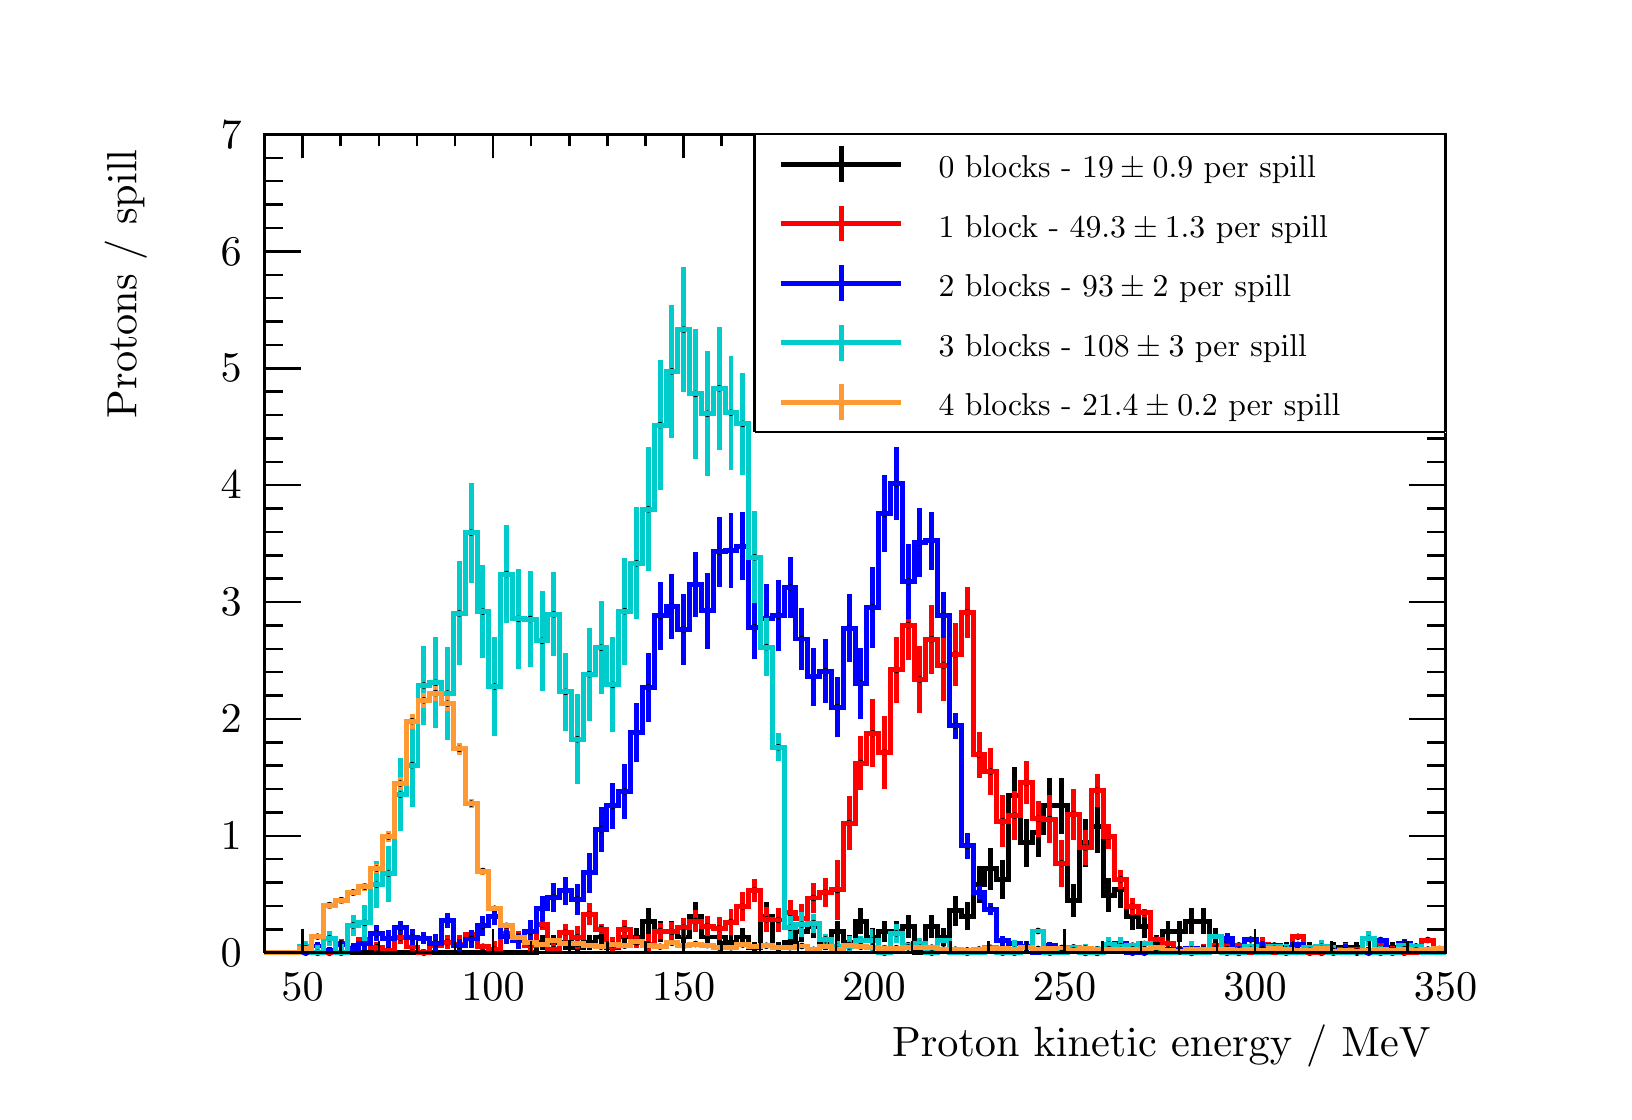
\begin{tikzpicture}
\pgfdeclareplotmark{cross} {
\pgfpathmoveto{\pgfpoint{-0.3\pgfplotmarksize}{\pgfplotmarksize}}
\pgfpathlineto{\pgfpoint{+0.3\pgfplotmarksize}{\pgfplotmarksize}}
\pgfpathlineto{\pgfpoint{+0.3\pgfplotmarksize}{0.3\pgfplotmarksize}}
\pgfpathlineto{\pgfpoint{+1\pgfplotmarksize}{0.3\pgfplotmarksize}}
\pgfpathlineto{\pgfpoint{+1\pgfplotmarksize}{-0.3\pgfplotmarksize}}
\pgfpathlineto{\pgfpoint{+0.3\pgfplotmarksize}{-0.3\pgfplotmarksize}}
\pgfpathlineto{\pgfpoint{+0.3\pgfplotmarksize}{-1.\pgfplotmarksize}}
\pgfpathlineto{\pgfpoint{-0.3\pgfplotmarksize}{-1.\pgfplotmarksize}}
\pgfpathlineto{\pgfpoint{-0.3\pgfplotmarksize}{-0.3\pgfplotmarksize}}
\pgfpathlineto{\pgfpoint{-1.\pgfplotmarksize}{-0.3\pgfplotmarksize}}
\pgfpathlineto{\pgfpoint{-1.\pgfplotmarksize}{0.3\pgfplotmarksize}}
\pgfpathlineto{\pgfpoint{-0.3\pgfplotmarksize}{0.3\pgfplotmarksize}}
\pgfpathclose
\pgfusepathqstroke
}
\pgfdeclareplotmark{cross*} {
\pgfpathmoveto{\pgfpoint{-0.3\pgfplotmarksize}{\pgfplotmarksize}}
\pgfpathlineto{\pgfpoint{+0.3\pgfplotmarksize}{\pgfplotmarksize}}
\pgfpathlineto{\pgfpoint{+0.3\pgfplotmarksize}{0.3\pgfplotmarksize}}
\pgfpathlineto{\pgfpoint{+1\pgfplotmarksize}{0.3\pgfplotmarksize}}
\pgfpathlineto{\pgfpoint{+1\pgfplotmarksize}{-0.3\pgfplotmarksize}}
\pgfpathlineto{\pgfpoint{+0.3\pgfplotmarksize}{-0.3\pgfplotmarksize}}
\pgfpathlineto{\pgfpoint{+0.3\pgfplotmarksize}{-1.\pgfplotmarksize}}
\pgfpathlineto{\pgfpoint{-0.3\pgfplotmarksize}{-1.\pgfplotmarksize}}
\pgfpathlineto{\pgfpoint{-0.3\pgfplotmarksize}{-0.3\pgfplotmarksize}}
\pgfpathlineto{\pgfpoint{-1.\pgfplotmarksize}{-0.3\pgfplotmarksize}}
\pgfpathlineto{\pgfpoint{-1.\pgfplotmarksize}{0.3\pgfplotmarksize}}
\pgfpathlineto{\pgfpoint{-0.3\pgfplotmarksize}{0.3\pgfplotmarksize}}
\pgfpathclose
\pgfusepathqfillstroke
}
\pgfdeclareplotmark{newstar} {
\pgfpathmoveto{\pgfqpoint{0pt}{\pgfplotmarksize}}
\pgfpathlineto{\pgfqpointpolar{44}{0.5\pgfplotmarksize}}
\pgfpathlineto{\pgfqpointpolar{18}{\pgfplotmarksize}}
\pgfpathlineto{\pgfqpointpolar{-20}{0.5\pgfplotmarksize}}
\pgfpathlineto{\pgfqpointpolar{-54}{\pgfplotmarksize}}
\pgfpathlineto{\pgfqpointpolar{-90}{0.5\pgfplotmarksize}}
\pgfpathlineto{\pgfqpointpolar{234}{\pgfplotmarksize}}
\pgfpathlineto{\pgfqpointpolar{198}{0.5\pgfplotmarksize}}
\pgfpathlineto{\pgfqpointpolar{162}{\pgfplotmarksize}}
\pgfpathlineto{\pgfqpointpolar{134}{0.5\pgfplotmarksize}}
\pgfpathclose
\pgfusepathqstroke
}
\pgfdeclareplotmark{newstar*} {
\pgfpathmoveto{\pgfqpoint{0pt}{\pgfplotmarksize}}
\pgfpathlineto{\pgfqpointpolar{44}{0.5\pgfplotmarksize}}
\pgfpathlineto{\pgfqpointpolar{18}{\pgfplotmarksize}}
\pgfpathlineto{\pgfqpointpolar{-20}{0.5\pgfplotmarksize}}
\pgfpathlineto{\pgfqpointpolar{-54}{\pgfplotmarksize}}
\pgfpathlineto{\pgfqpointpolar{-90}{0.5\pgfplotmarksize}}
\pgfpathlineto{\pgfqpointpolar{234}{\pgfplotmarksize}}
\pgfpathlineto{\pgfqpointpolar{198}{0.5\pgfplotmarksize}}
\pgfpathlineto{\pgfqpointpolar{162}{\pgfplotmarksize}}
\pgfpathlineto{\pgfqpointpolar{134}{0.5\pgfplotmarksize}}
\pgfpathclose
\pgfusepathqfillstroke
}
\definecolor{c}{rgb}{1,1,1};
\draw [color=c, fill=c] (0,0) rectangle (20,13.4957);
\draw [color=c, fill=c] (3,1.75444) rectangle (18,12.1461);
\definecolor{c}{rgb}{0,0,0};
\draw [c,line width=0.9] (3,1.75444) -- (3,12.1461) -- (18,12.1461) -- (18,1.75444) -- (3,1.75444);
\definecolor{c}{rgb}{1,1,1};
\draw [color=c, fill=c] (3,1.75444) rectangle (18,12.1461);
\definecolor{c}{rgb}{0,0,0};
\draw [c,line width=0.9] (3,1.75444) -- (3,12.1461) -- (18,12.1461) -- (18,1.75444) -- (3,1.75444);
\draw [c,line width=0.9] (3,1.75444) -- (3.15,1.75444) -- (3.15,1.75444) -- (3.3,1.75444) -- (3.3,1.75444) -- (3.45,1.75444) -- (3.45,1.75444) -- (3.6,1.75444) -- (3.6,1.75444) -- (3.75,1.75444) -- (3.75,1.75444) -- (3.9,1.75444) -- (3.9,1.75444) --
 (4.05,1.75444) -- (4.05,1.75444) -- (4.2,1.75444) -- (4.2,1.75444) -- (4.35,1.75444) -- (4.35,1.75444) -- (4.5,1.75444) -- (4.5,1.75444) -- (4.65,1.75444) -- (4.65,1.75444) -- (4.8,1.75444) -- (4.8,1.75444) -- (4.95,1.75444) -- (4.95,1.75444) --
 (5.1,1.75444) -- (5.1,1.75444) -- (5.25,1.75444) -- (5.25,1.75444) -- (5.4,1.75444) -- (5.4,1.75444) -- (5.55,1.75444) -- (5.55,1.75444) -- (5.7,1.75444) -- (5.7,1.75444) -- (5.85,1.75444) -- (5.85,1.75444) -- (6,1.75444) -- (6,1.75444) --
 (6.15,1.75444) -- (6.15,1.75444) -- (6.3,1.75444) -- (6.3,1.75444) -- (6.45,1.75444) -- (6.45,1.75444) -- (6.6,1.75444) -- (6.6,1.75444) -- (6.75,1.75444) -- (6.75,1.75444) -- (6.9,1.75444) -- (6.9,1.75444) -- (7.05,1.75444) -- (7.05,1.75444) --
 (7.2,1.75444) -- (7.2,1.75444) -- (7.35,1.75444) -- (7.35,1.75444) -- (7.5,1.75444) -- (7.5,1.75444) -- (7.65,1.75444) -- (7.65,1.75444) -- (7.8,1.75444) -- (7.8,1.75444) -- (7.95,1.75444) -- (7.95,1.75444) -- (8.1,1.75444) -- (8.1,1.75444) --
 (8.25,1.75444) -- (8.25,1.75444) -- (8.4,1.75444) -- (8.4,1.75444) -- (8.55,1.75444) -- (8.55,1.75444) -- (8.7,1.75444) -- (8.7,1.75444) -- (8.85,1.75444) -- (8.85,1.75444) -- (9,1.75444) -- (9,1.75444) -- (9.15,1.75444) -- (9.15,1.75444) --
 (9.3,1.75444) -- (9.3,1.75444) -- (9.45,1.75444) -- (9.45,1.75444) -- (9.6,1.75444) -- (9.6,1.75444) -- (9.75,1.75444) -- (9.75,1.75444) -- (9.9,1.75444) -- (9.9,1.75444) -- (10.05,1.75444) -- (10.05,1.75444) -- (10.2,1.75444) -- (10.2,1.75444) --
 (10.35,1.75444) -- (10.35,1.75444) -- (10.5,1.75444) -- (10.5,1.75444) -- (10.65,1.75444) -- (10.65,1.75444) -- (10.8,1.75444) -- (10.8,1.75444) -- (10.95,1.75444) -- (10.95,1.75444) -- (11.1,1.75444) -- (11.1,1.75444) -- (11.25,1.75444) --
 (11.25,1.75444) -- (11.4,1.75444) -- (11.4,1.75444) -- (11.55,1.75444) -- (11.55,1.75444) -- (11.7,1.75444) -- (11.7,1.75444) -- (11.85,1.75444) -- (11.85,1.75444) -- (12,1.75444) -- (12,1.75444) -- (12.15,1.75444) -- (12.15,1.75444) --
 (12.3,1.75444) -- (12.3,1.75444) -- (12.45,1.75444) -- (12.45,1.75444) -- (12.6,1.75444) -- (12.6,1.75444) -- (12.75,1.75444) -- (12.75,1.75444) -- (12.9,1.75444) -- (12.9,1.75444) -- (13.05,1.75444) -- (13.05,1.75444) -- (13.2,1.75444) --
 (13.2,1.75444) -- (13.35,1.75444) -- (13.35,1.75444) -- (13.5,1.75444) -- (13.5,1.75444) -- (13.65,1.75444) -- (13.65,1.75444) -- (13.8,1.75444) -- (13.8,1.75444) -- (13.95,1.75444) -- (13.95,1.75444) -- (14.1,1.75444) -- (14.1,1.75444) --
 (14.25,1.75444) -- (14.25,1.75444) -- (14.4,1.75444) -- (14.4,1.75444) -- (14.55,1.75444) -- (14.55,1.75444) -- (14.7,1.75444) -- (14.7,1.75444) -- (14.85,1.75444) -- (14.85,1.75444) -- (15,1.75444) -- (15,1.75444) -- (15.15,1.75444) --
 (15.15,1.75444) -- (15.3,1.75444) -- (15.3,1.75444) -- (15.45,1.75444) -- (15.45,1.75444) -- (15.6,1.75444) -- (15.6,1.75444) -- (15.75,1.75444) -- (15.75,1.75444) -- (15.9,1.75444) -- (15.9,1.75444) -- (16.05,1.75444) -- (16.05,1.75444) --
 (16.2,1.75444) -- (16.2,1.75444) -- (16.35,1.75444) -- (16.35,1.75444) -- (16.5,1.75444) -- (16.5,1.75444) -- (16.65,1.75444) -- (16.65,1.75444) -- (16.8,1.75444) -- (16.8,1.75444) -- (16.95,1.75444) -- (16.95,1.75444) -- (17.1,1.75444) --
 (17.1,1.75444) -- (17.25,1.75444) -- (17.25,1.75444) -- (17.4,1.75444) -- (17.4,1.75444) -- (17.55,1.75444) -- (17.55,1.75444) -- (17.7,1.75444) -- (17.7,1.75444) -- (17.85,1.75444) -- (17.85,1.75444) -- (18,1.75444);
\draw [c,line width=0.9] (3,1.75444) -- (18,1.75444);
\draw [c,line width=0.9] (3.48387,2.05809) -- (3.48387,1.75444);
\draw [c,line width=0.9] (3.96774,1.90627) -- (3.96774,1.75444);
\draw [c,line width=0.9] (4.45161,1.90627) -- (4.45161,1.75444);
\draw [c,line width=0.9] (4.93548,1.90627) -- (4.93548,1.75444);
\draw [c,line width=0.9] (5.41935,1.90627) -- (5.41935,1.75444);
\draw [c,line width=0.9] (5.90323,2.05809) -- (5.90323,1.75444);
\draw [c,line width=0.9] (6.3871,1.90627) -- (6.3871,1.75444);
\draw [c,line width=0.9] (6.87097,1.90627) -- (6.87097,1.75444);
\draw [c,line width=0.9] (7.35484,1.90627) -- (7.35484,1.75444);
\draw [c,line width=0.9] (7.83871,1.90627) -- (7.83871,1.75444);
\draw [c,line width=0.9] (8.32258,2.05809) -- (8.32258,1.75444);
\draw [c,line width=0.9] (8.80645,1.90627) -- (8.80645,1.75444);
\draw [c,line width=0.9] (9.29032,1.90627) -- (9.29032,1.75444);
\draw [c,line width=0.9] (9.77419,1.90627) -- (9.77419,1.75444);
\draw [c,line width=0.9] (10.2581,1.90627) -- (10.2581,1.75444);
\draw [c,line width=0.9] (10.7419,2.05809) -- (10.7419,1.75444);
\draw [c,line width=0.9] (11.2258,1.90627) -- (11.2258,1.75444);
\draw [c,line width=0.9] (11.7097,1.90627) -- (11.7097,1.75444);
\draw [c,line width=0.9] (12.1935,1.90627) -- (12.1935,1.75444);
\draw [c,line width=0.9] (12.6774,1.90627) -- (12.6774,1.75444);
\draw [c,line width=0.9] (13.1613,2.05809) -- (13.1613,1.75444);
\draw [c,line width=0.9] (13.6452,1.90627) -- (13.6452,1.75444);
\draw [c,line width=0.9] (14.129,1.90627) -- (14.129,1.75444);
\draw [c,line width=0.9] (14.6129,1.90627) -- (14.6129,1.75444);
\draw [c,line width=0.9] (15.0968,1.90627) -- (15.0968,1.75444);
\draw [c,line width=0.9] (15.5806,2.05809) -- (15.5806,1.75444);
\draw [c,line width=0.9] (16.0645,1.90627) -- (16.0645,1.75444);
\draw [c,line width=0.9] (16.5484,1.90627) -- (16.5484,1.75444);
\draw [c,line width=0.9] (17.0323,1.90627) -- (17.0323,1.75444);
\draw [c,line width=0.9] (17.5161,1.90627) -- (17.5161,1.75444);
\draw [c,line width=0.9] (18,2.05809) -- (18,1.75444);
\draw [c,line width=0.9] (3.48387,2.05809) -- (3.48387,1.75444);
\draw [c,line width=0.9] (18,2.05809) -- (18,1.75444);
\draw [anchor=base] (3.48387,1.14713) node[scale=1.52731, color=c, rotate=0]{50};
\draw [anchor=base] (5.90323,1.14713) node[scale=1.52731, color=c, rotate=0]{100};
\draw [anchor=base] (8.32258,1.14713) node[scale=1.52731, color=c, rotate=0]{150};
\draw [anchor=base] (10.7419,1.14713) node[scale=1.52731, color=c, rotate=0]{200};
\draw [anchor=base] (13.1613,1.14713) node[scale=1.52731, color=c, rotate=0]{250};
\draw [anchor=base] (15.5806,1.14713) node[scale=1.52731, color=c, rotate=0]{300};
\draw [anchor=base] (18,1.14713) node[scale=1.52731, color=c, rotate=0]{350};
\draw [anchor= east] (18,0.566819) node[scale=1.52731, color=c, rotate=0]{ Proton kinetic energy / MeV};
\draw [c,line width=0.9] (3,12.1461) -- (18,12.1461);
\draw [c,line width=0.9] (3.48387,11.8425) -- (3.48387,12.1461);
\draw [c,line width=0.9] (3.96774,11.9943) -- (3.96774,12.1461);
\draw [c,line width=0.9] (4.45161,11.9943) -- (4.45161,12.1461);
\draw [c,line width=0.9] (4.93548,11.9943) -- (4.93548,12.1461);
\draw [c,line width=0.9] (5.41935,11.9943) -- (5.41935,12.1461);
\draw [c,line width=0.9] (5.90323,11.8425) -- (5.90323,12.1461);
\draw [c,line width=0.9] (6.3871,11.9943) -- (6.3871,12.1461);
\draw [c,line width=0.9] (6.87097,11.9943) -- (6.87097,12.1461);
\draw [c,line width=0.9] (7.35484,11.9943) -- (7.35484,12.1461);
\draw [c,line width=0.9] (7.83871,11.9943) -- (7.83871,12.1461);
\draw [c,line width=0.9] (8.32258,11.8425) -- (8.32258,12.1461);
\draw [c,line width=0.9] (8.80645,11.9943) -- (8.80645,12.1461);
\draw [c,line width=0.9] (9.29032,11.9943) -- (9.29032,12.1461);
\draw [c,line width=0.9] (9.77419,11.9943) -- (9.77419,12.1461);
\draw [c,line width=0.9] (10.2581,11.9943) -- (10.2581,12.1461);
\draw [c,line width=0.9] (10.7419,11.8425) -- (10.7419,12.1461);
\draw [c,line width=0.9] (11.2258,11.9943) -- (11.2258,12.1461);
\draw [c,line width=0.9] (11.7097,11.9943) -- (11.7097,12.1461);
\draw [c,line width=0.9] (12.1935,11.9943) -- (12.1935,12.1461);
\draw [c,line width=0.9] (12.6774,11.9943) -- (12.6774,12.1461);
\draw [c,line width=0.9] (13.1613,11.8425) -- (13.1613,12.1461);
\draw [c,line width=0.9] (13.6452,11.9943) -- (13.6452,12.1461);
\draw [c,line width=0.9] (14.129,11.9943) -- (14.129,12.1461);
\draw [c,line width=0.9] (14.6129,11.9943) -- (14.6129,12.1461);
\draw [c,line width=0.9] (15.0968,11.9943) -- (15.0968,12.1461);
\draw [c,line width=0.9] (15.5806,11.8425) -- (15.5806,12.1461);
\draw [c,line width=0.9] (16.0645,11.9943) -- (16.0645,12.1461);
\draw [c,line width=0.9] (16.5484,11.9943) -- (16.5484,12.1461);
\draw [c,line width=0.9] (17.0323,11.9943) -- (17.0323,12.1461);
\draw [c,line width=0.9] (17.5161,11.9943) -- (17.5161,12.1461);
\draw [c,line width=0.9] (18,11.8425) -- (18,12.1461);
\draw [c,line width=0.9] (3.48387,11.8425) -- (3.48387,12.1461);
\draw [c,line width=0.9] (18,11.8425) -- (18,12.1461);
\draw [c,line width=0.9] (3,1.75444) -- (3,12.1461);
\draw [c,line width=0.9] (3.462,1.75444) -- (3,1.75444);
\draw [c,line width=0.9] (3.231,2.05135) -- (3,2.05135);
\draw [c,line width=0.9] (3.231,2.34825) -- (3,2.34825);
\draw [c,line width=0.9] (3.231,2.64516) -- (3,2.64516);
\draw [c,line width=0.9] (3.231,2.94206) -- (3,2.94206);
\draw [c,line width=0.9] (3.462,3.23897) -- (3,3.23897);
\draw [c,line width=0.9] (3.231,3.53587) -- (3,3.53587);
\draw [c,line width=0.9] (3.231,3.83278) -- (3,3.83278);
\draw [c,line width=0.9] (3.231,4.12968) -- (3,4.12968);
\draw [c,line width=0.9] (3.231,4.42659) -- (3,4.42659);
\draw [c,line width=0.9] (3.462,4.7235) -- (3,4.7235);
\draw [c,line width=0.9] (3.231,5.0204) -- (3,5.0204);
\draw [c,line width=0.9] (3.231,5.31731) -- (3,5.31731);
\draw [c,line width=0.9] (3.231,5.61421) -- (3,5.61421);
\draw [c,line width=0.9] (3.231,5.91112) -- (3,5.91112);
\draw [c,line width=0.9] (3.462,6.20802) -- (3,6.20802);
\draw [c,line width=0.9] (3.231,6.50493) -- (3,6.50493);
\draw [c,line width=0.9] (3.231,6.80183) -- (3,6.80183);
\draw [c,line width=0.9] (3.231,7.09874) -- (3,7.09874);
\draw [c,line width=0.9] (3.231,7.39564) -- (3,7.39564);
\draw [c,line width=0.9] (3.462,7.69255) -- (3,7.69255);
\draw [c,line width=0.9] (3.231,7.98946) -- (3,7.98946);
\draw [c,line width=0.9] (3.231,8.28636) -- (3,8.28636);
\draw [c,line width=0.9] (3.231,8.58327) -- (3,8.58327);
\draw [c,line width=0.9] (3.231,8.88017) -- (3,8.88017);
\draw [c,line width=0.9] (3.462,9.17708) -- (3,9.17708);
\draw [c,line width=0.9] (3.231,9.47398) -- (3,9.47398);
\draw [c,line width=0.9] (3.231,9.77089) -- (3,9.77089);
\draw [c,line width=0.9] (3.231,10.0678) -- (3,10.0678);
\draw [c,line width=0.9] (3.231,10.3647) -- (3,10.3647);
\draw [c,line width=0.9] (3.462,10.6616) -- (3,10.6616);
\draw [c,line width=0.9] (3.231,10.9585) -- (3,10.9585);
\draw [c,line width=0.9] (3.231,11.2554) -- (3,11.2554);
\draw [c,line width=0.9] (3.231,11.5523) -- (3,11.5523);
\draw [c,line width=0.9] (3.231,11.8492) -- (3,11.8492);
\draw [c,line width=0.9] (3.462,12.1461) -- (3,12.1461);
\draw [anchor= east] (2.9,1.75444) node[scale=1.52731, color=c, rotate=0]{0};
\draw [anchor= east] (2.9,3.23897) node[scale=1.52731, color=c, rotate=0]{1};
\draw [anchor= east] (2.9,4.7235) node[scale=1.52731, color=c, rotate=0]{2};
\draw [anchor= east] (2.9,6.20802) node[scale=1.52731, color=c, rotate=0]{3};
\draw [anchor= east] (2.9,7.69255) node[scale=1.52731, color=c, rotate=0]{4};
\draw [anchor= east] (2.9,9.17708) node[scale=1.52731, color=c, rotate=0]{5};
\draw [anchor= east] (2.9,10.6616) node[scale=1.52731, color=c, rotate=0]{6};
\draw [anchor= east] (2.9,12.1461) node[scale=1.52731, color=c, rotate=0]{7};
\draw [anchor= east] (1.24,12.1461) node[scale=1.52731, color=c, rotate=90]{ Protons / spill};
\draw [c,line width=0.9] (18,1.75444) -- (18,12.1461);
\draw [c,line width=0.9] (17.538,1.75444) -- (18,1.75444);
\draw [c,line width=0.9] (17.769,2.05135) -- (18,2.05135);
\draw [c,line width=0.9] (17.769,2.34825) -- (18,2.34825);
\draw [c,line width=0.9] (17.769,2.64516) -- (18,2.64516);
\draw [c,line width=0.9] (17.769,2.94206) -- (18,2.94206);
\draw [c,line width=0.9] (17.538,3.23897) -- (18,3.23897);
\draw [c,line width=0.9] (17.769,3.53587) -- (18,3.53587);
\draw [c,line width=0.9] (17.769,3.83278) -- (18,3.83278);
\draw [c,line width=0.9] (17.769,4.12968) -- (18,4.12968);
\draw [c,line width=0.9] (17.769,4.42659) -- (18,4.42659);
\draw [c,line width=0.9] (17.538,4.7235) -- (18,4.7235);
\draw [c,line width=0.9] (17.769,5.0204) -- (18,5.0204);
\draw [c,line width=0.9] (17.769,5.31731) -- (18,5.31731);
\draw [c,line width=0.9] (17.769,5.61421) -- (18,5.61421);
\draw [c,line width=0.9] (17.769,5.91112) -- (18,5.91112);
\draw [c,line width=0.9] (17.538,6.20802) -- (18,6.20802);
\draw [c,line width=0.9] (17.769,6.50493) -- (18,6.50493);
\draw [c,line width=0.9] (17.769,6.80183) -- (18,6.80183);
\draw [c,line width=0.9] (17.769,7.09874) -- (18,7.09874);
\draw [c,line width=0.9] (17.769,7.39564) -- (18,7.39564);
\draw [c,line width=0.9] (17.538,7.69255) -- (18,7.69255);
\draw [c,line width=0.9] (17.769,7.98946) -- (18,7.98946);
\draw [c,line width=0.9] (17.769,8.28636) -- (18,8.28636);
\draw [c,line width=0.9] (17.769,8.58327) -- (18,8.58327);
\draw [c,line width=0.9] (17.769,8.88017) -- (18,8.88017);
\draw [c,line width=0.9] (17.538,9.17708) -- (18,9.17708);
\draw [c,line width=0.9] (17.769,9.47398) -- (18,9.47398);
\draw [c,line width=0.9] (17.769,9.77089) -- (18,9.77089);
\draw [c,line width=0.9] (17.769,10.0678) -- (18,10.0678);
\draw [c,line width=0.9] (17.769,10.3647) -- (18,10.3647);
\draw [c,line width=0.9] (17.538,10.6616) -- (18,10.6616);
\draw [c,line width=0.9] (17.769,10.9585) -- (18,10.9585);
\draw [c,line width=0.9] (17.769,11.2554) -- (18,11.2554);
\draw [c,line width=0.9] (17.769,11.5523) -- (18,11.5523);
\draw [c,line width=0.9] (17.769,11.8492) -- (18,11.8492);
\draw [c,line width=0.9] (17.538,12.1461) -- (18,12.1461);
\draw [c,line width=1.8] (6.525,1.79346) -- (6.525,1.88768);
\draw [c,line width=1.8] (6.525,1.88768) -- (6.525,1.9819);
\foreach \P in {(6.525,1.88768)}{\draw[mark options={color=c,fill=c},mark size=2.402402pt,mark=*,mark size=1pt] plot coordinates {\P};}
\draw [c,line width=1.8] (6.675,1.79346) -- (6.675,1.88768);
\draw [c,line width=1.8] (6.675,1.88768) -- (6.675,1.9819);
\foreach \P in {(6.675,1.88768)}{\draw[mark options={color=c,fill=c},mark size=2.402402pt,mark=*,mark size=1pt] plot coordinates {\P};}
\draw [c,line width=1.8] (6.825,1.79346) -- (6.825,1.88768);
\draw [c,line width=1.8] (6.825,1.88768) -- (6.825,1.9819);
\foreach \P in {(6.825,1.88768)}{\draw[mark options={color=c,fill=c},mark size=2.402402pt,mark=*,mark size=1pt] plot coordinates {\P};}
\draw [c,line width=1.8] (6.975,1.75444) -- (6.975,1.82106);
\draw [c,line width=1.8] (6.975,1.82106) -- (6.975,1.88769);
\foreach \P in {(6.975,1.82106)}{\draw[mark options={color=c,fill=c},mark size=2.402402pt,mark=*,mark size=1pt] plot coordinates {\P};}
\draw [c,line width=1.8] (7.125,1.79346) -- (7.125,1.88768);
\draw [c,line width=1.8] (7.125,1.88768) -- (7.125,1.9819);
\foreach \P in {(7.125,1.88768)}{\draw[mark options={color=c,fill=c},mark size=2.402402pt,mark=*,mark size=1pt] plot coordinates {\P};}
\draw [c,line width=1.8] (7.275,1.83891) -- (7.275,1.9543);
\draw [c,line width=1.8] (7.275,1.9543) -- (7.275,2.0697);
\foreach \P in {(7.275,1.9543)}{\draw[mark options={color=c,fill=c},mark size=2.402402pt,mark=*,mark size=1pt] plot coordinates {\P};}
\draw [c,line width=1.8] (7.425,1.75444) -- (7.425,1.82106);
\draw [c,line width=1.8] (7.425,1.82106) -- (7.425,1.88769);
\foreach \P in {(7.425,1.82106)}{\draw[mark options={color=c,fill=c},mark size=2.402402pt,mark=*,mark size=1pt] plot coordinates {\P};}
\draw [c,line width=1.8] (7.575,1.83891) -- (7.575,1.9543);
\draw [c,line width=1.8] (7.575,1.9543) -- (7.575,2.0697);
\foreach \P in {(7.575,1.9543)}{\draw[mark options={color=c,fill=c},mark size=2.402402pt,mark=*,mark size=1pt] plot coordinates {\P};}
\draw [c,line width=1.8] (7.725,1.83891) -- (7.725,1.9543);
\draw [c,line width=1.8] (7.725,1.9543) -- (7.725,2.0697);
\foreach \P in {(7.725,1.9543)}{\draw[mark options={color=c,fill=c},mark size=2.402402pt,mark=*,mark size=1pt] plot coordinates {\P};}
\draw [c,line width=1.8] (7.875,1.99097) -- (7.875,2.15417);
\draw [c,line width=1.8] (7.875,2.15417) -- (7.875,2.31736);
\foreach \P in {(7.875,2.15417)}{\draw[mark options={color=c,fill=c},mark size=2.402402pt,mark=*,mark size=1pt] plot coordinates {\P};}
\draw [c,line width=1.8] (8.025,1.88767) -- (8.025,2.02092);
\draw [c,line width=1.8] (8.025,2.02092) -- (8.025,2.15417);
\foreach \P in {(8.025,2.02092)}{\draw[mark options={color=c,fill=c},mark size=2.402402pt,mark=*,mark size=1pt] plot coordinates {\P};}
\draw [c,line width=1.8] (8.175,1.88767) -- (8.175,2.02092);
\draw [c,line width=1.8] (8.175,2.02092) -- (8.175,2.15417);
\foreach \P in {(8.175,2.02092)}{\draw[mark options={color=c,fill=c},mark size=2.402402pt,mark=*,mark size=1pt] plot coordinates {\P};}
\draw [c,line width=1.8] (8.325,1.83891) -- (8.325,1.9543);
\draw [c,line width=1.8] (8.325,1.9543) -- (8.325,2.0697);
\foreach \P in {(8.325,1.9543)}{\draw[mark options={color=c,fill=c},mark size=2.402402pt,mark=*,mark size=1pt] plot coordinates {\P};}
\draw [c,line width=1.8] (8.475,2.04451) -- (8.475,2.22079);
\draw [c,line width=1.8] (8.475,2.22079) -- (8.475,2.39706);
\foreach \P in {(8.475,2.22079)}{\draw[mark options={color=c,fill=c},mark size=2.402402pt,mark=*,mark size=1pt] plot coordinates {\P};}
\draw [c,line width=1.8] (8.625,1.83891) -- (8.625,1.9543);
\draw [c,line width=1.8] (8.625,1.9543) -- (8.625,2.0697);
\foreach \P in {(8.625,1.9543)}{\draw[mark options={color=c,fill=c},mark size=2.402402pt,mark=*,mark size=1pt] plot coordinates {\P};}
\draw [c,line width=1.8] (8.775,1.83891) -- (8.775,1.9543);
\draw [c,line width=1.8] (8.775,1.9543) -- (8.775,2.0697);
\foreach \P in {(8.775,1.9543)}{\draw[mark options={color=c,fill=c},mark size=2.402402pt,mark=*,mark size=1pt] plot coordinates {\P};}
\draw [c,line width=1.8] (8.925,1.79346) -- (8.925,1.88768);
\draw [c,line width=1.8] (8.925,1.88768) -- (8.925,1.9819);
\foreach \P in {(8.925,1.88768)}{\draw[mark options={color=c,fill=c},mark size=2.402402pt,mark=*,mark size=1pt] plot coordinates {\P};}
\draw [c,line width=1.8] (9.075,1.83891) -- (9.075,1.9543);
\draw [c,line width=1.8] (9.075,1.9543) -- (9.075,2.0697);
\foreach \P in {(9.075,1.9543)}{\draw[mark options={color=c,fill=c},mark size=2.402402pt,mark=*,mark size=1pt] plot coordinates {\P};}
\draw [c,line width=1.8] (9.225,1.75444) -- (9.225,1.82106);
\draw [c,line width=1.8] (9.225,1.82106) -- (9.225,1.88769);
\foreach \P in {(9.225,1.82106)}{\draw[mark options={color=c,fill=c},mark size=2.402402pt,mark=*,mark size=1pt] plot coordinates {\P};}
\draw [c,line width=1.8] (9.375,2.04451) -- (9.375,2.22079);
\draw [c,line width=1.8] (9.375,2.22079) -- (9.375,2.39706);
\foreach \P in {(9.375,2.22079)}{\draw[mark options={color=c,fill=c},mark size=2.402402pt,mark=*,mark size=1pt] plot coordinates {\P};}
\draw [c,line width=1.8] (9.525,1.75444) -- (9.525,1.82106);
\draw [c,line width=1.8] (9.525,1.82106) -- (9.525,1.88769);
\foreach \P in {(9.525,1.82106)}{\draw[mark options={color=c,fill=c},mark size=2.402402pt,mark=*,mark size=1pt] plot coordinates {\P};}
\draw [c,line width=1.8] (9.675,1.79346) -- (9.675,1.88768);
\draw [c,line width=1.8] (9.675,1.88768) -- (9.675,1.9819);
\foreach \P in {(9.675,1.88768)}{\draw[mark options={color=c,fill=c},mark size=2.402402pt,mark=*,mark size=1pt] plot coordinates {\P};}
\draw [c,line width=1.8] (9.825,1.88767) -- (9.825,2.02092);
\draw [c,line width=1.8] (9.825,2.02092) -- (9.825,2.15417);
\foreach \P in {(9.825,2.02092)}{\draw[mark options={color=c,fill=c},mark size=2.402402pt,mark=*,mark size=1pt] plot coordinates {\P};}
\draw [c,line width=1.8] (9.975,1.93857) -- (9.975,2.08755);
\draw [c,line width=1.8] (9.975,2.08755) -- (9.975,2.23652);
\foreach \P in {(9.975,2.08755)}{\draw[mark options={color=c,fill=c},mark size=2.402402pt,mark=*,mark size=1pt] plot coordinates {\P};}
\draw [c,line width=1.8] (10.125,1.79346) -- (10.125,1.88768);
\draw [c,line width=1.8] (10.125,1.88768) -- (10.125,1.9819);
\foreach \P in {(10.125,1.88768)}{\draw[mark options={color=c,fill=c},mark size=2.402402pt,mark=*,mark size=1pt] plot coordinates {\P};}
\draw [c,line width=1.8] (10.275,1.88767) -- (10.275,2.02092);
\draw [c,line width=1.8] (10.275,2.02092) -- (10.275,2.15417);
\foreach \P in {(10.275,2.02092)}{\draw[mark options={color=c,fill=c},mark size=2.402402pt,mark=*,mark size=1pt] plot coordinates {\P};}
\draw [c,line width=1.8] (10.425,1.79346) -- (10.425,1.88768);
\draw [c,line width=1.8] (10.425,1.88768) -- (10.425,1.9819);
\foreach \P in {(10.425,1.88768)}{\draw[mark options={color=c,fill=c},mark size=2.402402pt,mark=*,mark size=1pt] plot coordinates {\P};}
\draw [c,line width=1.8] (10.575,1.99097) -- (10.575,2.15417);
\draw [c,line width=1.8] (10.575,2.15417) -- (10.575,2.31736);
\foreach \P in {(10.575,2.15417)}{\draw[mark options={color=c,fill=c},mark size=2.402402pt,mark=*,mark size=1pt] plot coordinates {\P};}
\draw [c,line width=1.8] (10.725,1.83891) -- (10.725,1.9543);
\draw [c,line width=1.8] (10.725,1.9543) -- (10.725,2.0697);
\foreach \P in {(10.725,1.9543)}{\draw[mark options={color=c,fill=c},mark size=2.402402pt,mark=*,mark size=1pt] plot coordinates {\P};}
\draw [c,line width=1.8] (10.875,1.88767) -- (10.875,2.02092);
\draw [c,line width=1.8] (10.875,2.02092) -- (10.875,2.15417);
\foreach \P in {(10.875,2.02092)}{\draw[mark options={color=c,fill=c},mark size=2.402402pt,mark=*,mark size=1pt] plot coordinates {\P};}
\draw [c,line width=1.8] (11.025,1.88767) -- (11.025,2.02092);
\draw [c,line width=1.8] (11.025,2.02092) -- (11.025,2.15417);
\foreach \P in {(11.025,2.02092)}{\draw[mark options={color=c,fill=c},mark size=2.402402pt,mark=*,mark size=1pt] plot coordinates {\P};}
\draw [c,line width=1.8] (11.175,1.93857) -- (11.175,2.08755);
\draw [c,line width=1.8] (11.175,2.08755) -- (11.175,2.23652);
\foreach \P in {(11.175,2.08755)}{\draw[mark options={color=c,fill=c},mark size=2.402402pt,mark=*,mark size=1pt] plot coordinates {\P};}
\draw [c,line width=1.8] (11.475,1.93857) -- (11.475,2.08755);
\draw [c,line width=1.8] (11.475,2.08755) -- (11.475,2.23652);
\foreach \P in {(11.475,2.08755)}{\draw[mark options={color=c,fill=c},mark size=2.402402pt,mark=*,mark size=1pt] plot coordinates {\P};}
\draw [c,line width=1.8] (11.625,1.83891) -- (11.625,1.9543);
\draw [c,line width=1.8] (11.625,1.9543) -- (11.625,2.0697);
\foreach \P in {(11.625,1.9543)}{\draw[mark options={color=c,fill=c},mark size=2.402402pt,mark=*,mark size=1pt] plot coordinates {\P};}
\draw [c,line width=1.8] (11.775,2.09896) -- (11.775,2.28741);
\draw [c,line width=1.8] (11.775,2.28741) -- (11.775,2.47585);
\foreach \P in {(11.775,2.28741)}{\draw[mark options={color=c,fill=c},mark size=2.402402pt,mark=*,mark size=1pt] plot coordinates {\P};}
\draw [c,line width=1.8] (11.925,2.04451) -- (11.925,2.22079);
\draw [c,line width=1.8] (11.925,2.22079) -- (11.925,2.39706);
\foreach \P in {(11.925,2.22079)}{\draw[mark options={color=c,fill=c},mark size=2.402402pt,mark=*,mark size=1pt] plot coordinates {\P};}
\draw [c,line width=1.8] (12.075,2.38029) -- (12.075,2.62051);
\draw [c,line width=1.8] (12.075,2.62051) -- (12.075,2.86073);
\foreach \P in {(12.075,2.62051)}{\draw[mark options={color=c,fill=c},mark size=2.402402pt,mark=*,mark size=1pt] plot coordinates {\P};}
\draw [c,line width=1.8] (12.225,2.55387) -- (12.225,2.82037);
\draw [c,line width=1.8] (12.225,2.82037) -- (12.225,3.08687);
\foreach \P in {(12.225,2.82037)}{\draw[mark options={color=c,fill=c},mark size=2.402402pt,mark=*,mark size=1pt] plot coordinates {\P};}
\draw [c,line width=1.8] (12.375,2.43784) -- (12.375,2.68713);
\draw [c,line width=1.8] (12.375,2.68713) -- (12.375,2.93642);
\foreach \P in {(12.375,2.68713)}{\draw[mark options={color=c,fill=c},mark size=2.402402pt,mark=*,mark size=1pt] plot coordinates {\P};}
\draw [c,line width=1.8] (12.525,3.38815) -- (12.525,3.75307);
\draw [c,line width=1.8] (12.525,3.75307) -- (12.525,4.11799);
\foreach \P in {(12.525,3.75307)}{\draw[mark options={color=c,fill=c},mark size=2.402402pt,mark=*,mark size=1pt] plot coordinates {\P};}
\draw [c,line width=1.8] (12.675,2.84816) -- (12.675,3.15348);
\draw [c,line width=1.8] (12.675,3.15348) -- (12.675,3.45879);
\foreach \P in {(12.675,3.15348)}{\draw[mark options={color=c,fill=c},mark size=2.402402pt,mark=*,mark size=1pt] plot coordinates {\P};}
\draw [c,line width=1.8] (12.825,2.9672) -- (12.825,3.28672);
\draw [c,line width=1.8] (12.825,3.28672) -- (12.825,3.60624);
\foreach \P in {(12.825,3.28672)}{\draw[mark options={color=c,fill=c},mark size=2.402402pt,mark=*,mark size=1pt] plot coordinates {\P};}
\draw [c,line width=1.8] (12.975,3.26728) -- (12.975,3.61982);
\draw [c,line width=1.8] (12.975,3.61982) -- (12.975,3.97237);
\foreach \P in {(12.975,3.61982)}{\draw[mark options={color=c,fill=c},mark size=2.402402pt,mark=*,mark size=1pt] plot coordinates {\P};}
\draw [c,line width=1.8] (13.125,3.26728) -- (13.125,3.61982);
\draw [c,line width=1.8] (13.125,3.61982) -- (13.125,3.97237);
\foreach \P in {(13.125,3.61982)}{\draw[mark options={color=c,fill=c},mark size=2.402402pt,mark=*,mark size=1pt] plot coordinates {\P};}
\draw [c,line width=1.8] (13.275,2.20996) -- (13.275,2.42065);
\draw [c,line width=1.8] (13.275,2.42065) -- (13.275,2.63134);
\foreach \P in {(13.275,2.42065)}{\draw[mark options={color=c,fill=c},mark size=2.402402pt,mark=*,mark size=1pt] plot coordinates {\P};}
\draw [c,line width=1.8] (13.425,2.84816) -- (13.425,3.15348);
\draw [c,line width=1.8] (13.425,3.15348) -- (13.425,3.45879);
\foreach \P in {(13.425,3.15348)}{\draw[mark options={color=c,fill=c},mark size=2.402402pt,mark=*,mark size=1pt] plot coordinates {\P};}
\draw [c,line width=1.8] (13.575,3.02695) -- (13.575,3.35334);
\draw [c,line width=1.8] (13.575,3.35334) -- (13.575,3.67974);
\foreach \P in {(13.575,3.35334)}{\draw[mark options={color=c,fill=c},mark size=2.402402pt,mark=*,mark size=1pt] plot coordinates {\P};}
\draw [c,line width=1.8] (13.725,2.2663) -- (13.725,2.48727);
\draw [c,line width=1.8] (13.725,2.48727) -- (13.725,2.70824);
\foreach \P in {(13.725,2.48727)}{\draw[mark options={color=c,fill=c},mark size=2.402402pt,mark=*,mark size=1pt] plot coordinates {\P};}
\draw [c,line width=1.8] (13.875,2.3231) -- (13.875,2.55389);
\draw [c,line width=1.8] (13.875,2.55389) -- (13.875,2.78469);
\foreach \P in {(13.875,2.55389)}{\draw[mark options={color=c,fill=c},mark size=2.402402pt,mark=*,mark size=1pt] plot coordinates {\P};}
\draw [c,line width=1.8] (14.025,2.04451) -- (14.025,2.22079);
\draw [c,line width=1.8] (14.025,2.22079) -- (14.025,2.39706);
\foreach \P in {(14.025,2.22079)}{\draw[mark options={color=c,fill=c},mark size=2.402402pt,mark=*,mark size=1pt] plot coordinates {\P};}
\draw [c,line width=1.8] (14.175,1.93857) -- (14.175,2.08755);
\draw [c,line width=1.8] (14.175,2.08755) -- (14.175,2.23652);
\foreach \P in {(14.175,2.08755)}{\draw[mark options={color=c,fill=c},mark size=2.402402pt,mark=*,mark size=1pt] plot coordinates {\P};}
\draw [c,line width=1.8] (14.325,1.79346) -- (14.325,1.88768);
\draw [c,line width=1.8] (14.325,1.88768) -- (14.325,1.9819);
\foreach \P in {(14.325,1.88768)}{\draw[mark options={color=c,fill=c},mark size=2.402402pt,mark=*,mark size=1pt] plot coordinates {\P};}
\draw [c,line width=1.8] (14.475,1.88767) -- (14.475,2.02092);
\draw [c,line width=1.8] (14.475,2.02092) -- (14.475,2.15417);
\foreach \P in {(14.475,2.02092)}{\draw[mark options={color=c,fill=c},mark size=2.402402pt,mark=*,mark size=1pt] plot coordinates {\P};}
\draw [c,line width=1.8] (14.625,1.88767) -- (14.625,2.02092);
\draw [c,line width=1.8] (14.625,2.02092) -- (14.625,2.15417);
\foreach \P in {(14.625,2.02092)}{\draw[mark options={color=c,fill=c},mark size=2.402402pt,mark=*,mark size=1pt] plot coordinates {\P};}
\draw [c,line width=1.8] (14.775,1.99097) -- (14.775,2.15417);
\draw [c,line width=1.8] (14.775,2.15417) -- (14.775,2.31736);
\foreach \P in {(14.775,2.15417)}{\draw[mark options={color=c,fill=c},mark size=2.402402pt,mark=*,mark size=1pt] plot coordinates {\P};}
\draw [c,line width=1.8] (14.925,1.99097) -- (14.925,2.15417);
\draw [c,line width=1.8] (14.925,2.15417) -- (14.925,2.31736);
\foreach \P in {(14.925,2.15417)}{\draw[mark options={color=c,fill=c},mark size=2.402402pt,mark=*,mark size=1pt] plot coordinates {\P};}
\draw [c,line width=1.8] (15.075,1.83891) -- (15.075,1.9543);
\draw [c,line width=1.8] (15.075,1.9543) -- (15.075,2.0697);
\foreach \P in {(15.075,1.9543)}{\draw[mark options={color=c,fill=c},mark size=2.402402pt,mark=*,mark size=1pt] plot coordinates {\P};}
\draw [c,line width=1.8] (15.225,1.79346) -- (15.225,1.88768);
\draw [c,line width=1.8] (15.225,1.88768) -- (15.225,1.9819);
\foreach \P in {(15.225,1.88768)}{\draw[mark options={color=c,fill=c},mark size=2.402402pt,mark=*,mark size=1pt] plot coordinates {\P};}
\draw [c,line width=1.8] (15.975,1.75444) -- (15.975,1.82106);
\draw [c,line width=1.8] (15.975,1.82106) -- (15.975,1.88769);
\foreach \P in {(15.975,1.82106)}{\draw[mark options={color=c,fill=c},mark size=2.402402pt,mark=*,mark size=1pt] plot coordinates {\P};}
\draw [c,line width=1.8] (16.275,1.75444) -- (16.275,1.82106);
\draw [c,line width=1.8] (16.275,1.82106) -- (16.275,1.88769);
\foreach \P in {(16.275,1.82106)}{\draw[mark options={color=c,fill=c},mark size=2.402402pt,mark=*,mark size=1pt] plot coordinates {\P};}
\draw [c,line width=1.8] (16.575,1.75444) -- (16.575,1.82106);
\draw [c,line width=1.8] (16.575,1.82106) -- (16.575,1.88769);
\foreach \P in {(16.575,1.82106)}{\draw[mark options={color=c,fill=c},mark size=2.402402pt,mark=*,mark size=1pt] plot coordinates {\P};}
\draw [c,line width=1.8] (16.725,1.75444) -- (16.725,1.82106);
\draw [c,line width=1.8] (16.725,1.82106) -- (16.725,1.88769);
\foreach \P in {(16.725,1.82106)}{\draw[mark options={color=c,fill=c},mark size=2.402402pt,mark=*,mark size=1pt] plot coordinates {\P};}
\draw [c,line width=1.8] (16.875,1.75444) -- (16.875,1.82106);
\draw [c,line width=1.8] (16.875,1.82106) -- (16.875,1.88769);
\foreach \P in {(16.875,1.82106)}{\draw[mark options={color=c,fill=c},mark size=2.402402pt,mark=*,mark size=1pt] plot coordinates {\P};}
\draw [c,line width=1.8] (17.175,1.75444) -- (17.175,1.82106);
\draw [c,line width=1.8] (17.175,1.82106) -- (17.175,1.88769);
\foreach \P in {(17.175,1.82106)}{\draw[mark options={color=c,fill=c},mark size=2.402402pt,mark=*,mark size=1pt] plot coordinates {\P};}
\draw [c,line width=1.8] (17.325,1.75444) -- (17.325,1.82106);
\draw [c,line width=1.8] (17.325,1.82106) -- (17.325,1.88769);
\foreach \P in {(17.325,1.82106)}{\draw[mark options={color=c,fill=c},mark size=2.402402pt,mark=*,mark size=1pt] plot coordinates {\P};}
\draw [c,line width=1.8] (3,1.75444) -- (3.15,1.75444) -- (3.15,1.75444) -- (3.3,1.75444) -- (3.3,1.75444) -- (3.45,1.75444) -- (3.45,1.75444) -- (3.6,1.75444) -- (3.6,1.75444) -- (3.75,1.75444) -- (3.75,1.75444) -- (3.9,1.75444) -- (3.9,1.75444) --
 (4.05,1.75444) -- (4.05,1.75444) -- (4.2,1.75444) -- (4.2,1.75444) -- (4.35,1.75444) -- (4.35,1.75444) -- (4.5,1.75444) -- (4.5,1.75444) -- (4.65,1.75444) -- (4.65,1.75444) -- (4.8,1.75444) -- (4.8,1.75444) -- (4.95,1.75444) -- (4.95,1.75444) --
 (5.1,1.75444) -- (5.1,1.75444) -- (5.25,1.75444) -- (5.25,1.75444) -- (5.4,1.75444) -- (5.4,1.75444) -- (5.55,1.75444) -- (5.55,1.75444) -- (5.7,1.75444) -- (5.7,1.75444) -- (5.85,1.75444) -- (5.85,1.75444) -- (6,1.75444) -- (6,1.75444) --
 (6.15,1.75444) -- (6.15,1.75444) -- (6.3,1.75444) -- (6.3,1.75444) -- (6.45,1.75444) -- (6.45,1.88768) -- (6.6,1.88768) -- (6.6,1.88768) -- (6.75,1.88768) -- (6.75,1.88768) -- (6.9,1.88768) -- (6.9,1.82106) -- (7.05,1.82106) -- (7.05,1.88768) --
 (7.2,1.88768) -- (7.2,1.9543) -- (7.35,1.9543) -- (7.35,1.82106) -- (7.5,1.82106) -- (7.5,1.9543) -- (7.65,1.9543) -- (7.65,1.9543) -- (7.8,1.9543) -- (7.8,2.15417) -- (7.95,2.15417) -- (7.95,2.02092) -- (8.1,2.02092) -- (8.1,2.02092) --
 (8.25,2.02092) -- (8.25,1.9543) -- (8.4,1.9543) -- (8.4,2.22079) -- (8.55,2.22079) -- (8.55,1.9543) -- (8.7,1.9543) -- (8.7,1.9543) -- (8.85,1.9543) -- (8.85,1.88768) -- (9,1.88768) -- (9,1.9543) -- (9.15,1.9543) -- (9.15,1.82106) -- (9.3,1.82106)
 -- (9.3,2.22079) -- (9.45,2.22079) -- (9.45,1.82106) -- (9.6,1.82106) -- (9.6,1.88768) -- (9.75,1.88768) -- (9.75,2.02092) -- (9.9,2.02092) -- (9.9,2.08755) -- (10.05,2.08755) -- (10.05,1.88768) -- (10.2,1.88768) -- (10.2,2.02092) -- (10.35,2.02092)
 -- (10.35,1.88768) -- (10.5,1.88768) -- (10.5,2.15417) -- (10.65,2.15417) -- (10.65,1.9543) -- (10.8,1.9543) -- (10.8,2.02092) -- (10.95,2.02092) -- (10.95,2.02092) -- (11.1,2.02092) -- (11.1,2.08755) -- (11.25,2.08755) -- (11.25,1.75444) --
 (11.4,1.75444) -- (11.4,2.08755) -- (11.55,2.08755) -- (11.55,1.9543) -- (11.7,1.9543) -- (11.7,2.28741) -- (11.85,2.28741) -- (11.85,2.22079) -- (12,2.22079) -- (12,2.62051) -- (12.15,2.62051) -- (12.15,2.82037) -- (12.3,2.82037) -- (12.3,2.68713)
 -- (12.45,2.68713) -- (12.45,3.75307) -- (12.6,3.75307) -- (12.6,3.15348) -- (12.75,3.15348) -- (12.75,3.28672) -- (12.9,3.28672) -- (12.9,3.61982) -- (13.05,3.61982) -- (13.05,3.61982) -- (13.2,3.61982) -- (13.2,2.42065) -- (13.35,2.42065) --
 (13.35,3.15348) -- (13.5,3.15348) -- (13.5,3.35334) -- (13.65,3.35334) -- (13.65,2.48727) -- (13.8,2.48727) -- (13.8,2.55389) -- (13.95,2.55389) -- (13.95,2.22079) -- (14.1,2.22079) -- (14.1,2.08755) -- (14.25,2.08755) -- (14.25,1.88768) --
 (14.4,1.88768) -- (14.4,2.02092) -- (14.55,2.02092) -- (14.55,2.02092) -- (14.7,2.02092) -- (14.7,2.15417) -- (14.85,2.15417) -- (14.85,2.15417) -- (15,2.15417) -- (15,1.9543) -- (15.15,1.9543) -- (15.15,1.88768) -- (15.3,1.88768) -- (15.3,1.75444)
 -- (15.45,1.75444) -- (15.45,1.75444) -- (15.6,1.75444) -- (15.6,1.75444) -- (15.75,1.75444) -- (15.75,1.75444) -- (15.9,1.75444) -- (15.9,1.82106) -- (16.05,1.82106) -- (16.05,1.75444) -- (16.2,1.75444) -- (16.2,1.82106) -- (16.35,1.82106) --
 (16.35,1.75444) -- (16.5,1.75444) -- (16.5,1.82106) -- (16.65,1.82106) -- (16.65,1.82106) -- (16.8,1.82106) -- (16.8,1.82106) -- (16.95,1.82106) -- (16.95,1.75444) -- (17.1,1.75444) -- (17.1,1.82106) -- (17.25,1.82106) -- (17.25,1.82106) --
 (17.4,1.82106) -- (17.4,1.75444) -- (17.55,1.75444) -- (17.55,1.75444) -- (17.7,1.75444) -- (17.7,1.75444) -- (17.85,1.75444) -- (17.85,1.75444) -- (18,1.75444);
\definecolor{c}{rgb}{1,0,0};
\draw [c,line width=1.8] (3.825,1.75444) -- (3.825,1.79985);
\definecolor{c}{rgb}{0,0,0};
\foreach \P in {(3.825,1.75444)}{\draw[mark options={color=c,fill=c},mark size=2.402402pt,mark=*,mark size=1pt] plot coordinates {\P};}
\definecolor{c}{rgb}{1,0,0};
\draw [c,line width=1.8] (3.975,1.82031) -- (3.975,1.87354);
\draw [c,line width=1.8] (3.975,1.87354) -- (3.975,1.92677);
\definecolor{c}{rgb}{0,0,0};
\foreach \P in {(3.975,1.87354)}{\draw[mark options={color=c,fill=c},mark size=2.402402pt,mark=*,mark size=1pt] plot coordinates {\P};}
\definecolor{c}{rgb}{1,0,0};
\draw [c,line width=1.8] (4.125,1.75444) -- (4.125,1.78432);
\draw [c,line width=1.8] (4.125,1.78432) -- (4.125,1.84824);
\definecolor{c}{rgb}{0,0,0};
\foreach \P in {(4.125,1.78432)}{\draw[mark options={color=c,fill=c},mark size=2.402402pt,mark=*,mark size=1pt] plot coordinates {\P};}
\definecolor{c}{rgb}{1,0,0};
\draw [c,line width=1.8] (4.275,1.84049) -- (4.275,1.92236);
\draw [c,line width=1.8] (4.275,1.92236) -- (4.275,2.00423);
\definecolor{c}{rgb}{0,0,0};
\foreach \P in {(4.275,1.92236)}{\draw[mark options={color=c,fill=c},mark size=2.402402pt,mark=*,mark size=1pt] plot coordinates {\P};}
\definecolor{c}{rgb}{1,0,0};
\draw [c,line width=1.8] (4.425,1.76305) -- (4.425,1.82446);
\draw [c,line width=1.8] (4.425,1.82446) -- (4.425,1.88588);
\definecolor{c}{rgb}{0,0,0};
\foreach \P in {(4.425,1.82446)}{\draw[mark options={color=c,fill=c},mark size=2.402402pt,mark=*,mark size=1pt] plot coordinates {\P};}
\definecolor{c}{rgb}{1,0,0};
\draw [c,line width=1.8] (4.575,1.75444) -- (4.575,1.7886);
\draw [c,line width=1.8] (4.575,1.7886) -- (4.575,1.84649);
\definecolor{c}{rgb}{0,0,0};
\foreach \P in {(4.575,1.7886)}{\draw[mark options={color=c,fill=c},mark size=2.402402pt,mark=*,mark size=1pt] plot coordinates {\P};}
\definecolor{c}{rgb}{1,0,0};
\draw [c,line width=1.8] (4.725,1.86769) -- (4.725,1.94838);
\draw [c,line width=1.8] (4.725,1.94838) -- (4.725,2.02906);
\definecolor{c}{rgb}{0,0,0};
\foreach \P in {(4.725,1.94838)}{\draw[mark options={color=c,fill=c},mark size=2.402402pt,mark=*,mark size=1pt] plot coordinates {\P};}
\definecolor{c}{rgb}{1,0,0};
\draw [c,line width=1.8] (4.875,1.77485) -- (4.875,1.82738);
\draw [c,line width=1.8] (4.875,1.82738) -- (4.875,1.87992);
\definecolor{c}{rgb}{0,0,0};
\foreach \P in {(4.875,1.82738)}{\draw[mark options={color=c,fill=c},mark size=2.402402pt,mark=*,mark size=1pt] plot coordinates {\P};}
\definecolor{c}{rgb}{1,0,0};
\draw [c,line width=1.8] (5.025,1.75444) -- (5.025,1.80022);
\definecolor{c}{rgb}{0,0,0};
\foreach \P in {(5.025,1.75444)}{\draw[mark options={color=c,fill=c},mark size=2.402402pt,mark=*,mark size=1pt] plot coordinates {\P};}
\definecolor{c}{rgb}{1,0,0};
\draw [c,line width=1.8] (5.175,1.79445) -- (5.175,1.85065);
\draw [c,line width=1.8] (5.175,1.85065) -- (5.175,1.90686);
\definecolor{c}{rgb}{0,0,0};
\foreach \P in {(5.175,1.85065)}{\draw[mark options={color=c,fill=c},mark size=2.402402pt,mark=*,mark size=1pt] plot coordinates {\P};}
\definecolor{c}{rgb}{1,0,0};
\draw [c,line width=1.8] (5.325,1.79732) -- (5.325,1.88864);
\draw [c,line width=1.8] (5.325,1.88864) -- (5.325,1.97996);
\definecolor{c}{rgb}{0,0,0};
\foreach \P in {(5.325,1.88864)}{\draw[mark options={color=c,fill=c},mark size=2.402402pt,mark=*,mark size=1pt] plot coordinates {\P};}
\definecolor{c}{rgb}{1,0,0};
\draw [c,line width=1.8] (5.475,1.75444) -- (5.475,1.86486);
\draw [c,line width=1.8] (5.475,1.86486) -- (5.475,1.98375);
\definecolor{c}{rgb}{0,0,0};
\foreach \P in {(5.475,1.86486)}{\draw[mark options={color=c,fill=c},mark size=2.402402pt,mark=*,mark size=1pt] plot coordinates {\P};}
\definecolor{c}{rgb}{1,0,0};
\draw [c,line width=1.8] (5.625,1.92581) -- (5.625,1.98113);
\draw [c,line width=1.8] (5.625,1.98113) -- (5.625,2.03645);
\definecolor{c}{rgb}{0,0,0};
\foreach \P in {(5.625,1.98113)}{\draw[mark options={color=c,fill=c},mark size=2.402402pt,mark=*,mark size=1pt] plot coordinates {\P};}
\definecolor{c}{rgb}{1,0,0};
\draw [c,line width=1.8] (5.775,1.79303) -- (5.775,1.8316);
\draw [c,line width=1.8] (5.775,1.8316) -- (5.775,1.87017);
\definecolor{c}{rgb}{0,0,0};
\foreach \P in {(5.775,1.8316)}{\draw[mark options={color=c,fill=c},mark size=2.402402pt,mark=*,mark size=1pt] plot coordinates {\P};}
\definecolor{c}{rgb}{1,0,0};
\draw [c,line width=1.8] (5.925,1.75444) -- (5.925,1.79263);
\draw [c,line width=1.8] (5.925,1.79263) -- (5.925,1.90444);
\definecolor{c}{rgb}{0,0,0};
\foreach \P in {(5.925,1.79263)}{\draw[mark options={color=c,fill=c},mark size=2.402402pt,mark=*,mark size=1pt] plot coordinates {\P};}
\definecolor{c}{rgb}{1,0,0};
\draw [c,line width=1.8] (6.075,1.91601) -- (6.075,1.99395);
\draw [c,line width=1.8] (6.075,1.99395) -- (6.075,2.07188);
\definecolor{c}{rgb}{0,0,0};
\foreach \P in {(6.075,1.99395)}{\draw[mark options={color=c,fill=c},mark size=2.402402pt,mark=*,mark size=1pt] plot coordinates {\P};}
\definecolor{c}{rgb}{1,0,0};
\draw [c,line width=1.8] (6.225,1.81659) -- (6.225,1.9212);
\draw [c,line width=1.8] (6.225,1.9212) -- (6.225,2.02582);
\definecolor{c}{rgb}{0,0,0};
\foreach \P in {(6.225,1.9212)}{\draw[mark options={color=c,fill=c},mark size=2.402402pt,mark=*,mark size=1pt] plot coordinates {\P};}
\definecolor{c}{rgb}{1,0,0};
\draw [c,line width=1.8] (6.375,1.75444) -- (6.375,1.8522);
\draw [c,line width=1.8] (6.375,1.8522) -- (6.375,1.96921);
\definecolor{c}{rgb}{0,0,0};
\foreach \P in {(6.375,1.8522)}{\draw[mark options={color=c,fill=c},mark size=2.402402pt,mark=*,mark size=1pt] plot coordinates {\P};}
\definecolor{c}{rgb}{1,0,0};
\draw [c,line width=1.8] (6.525,2.0386) -- (6.525,2.11242);
\draw [c,line width=1.8] (6.525,2.11242) -- (6.525,2.18624);
\definecolor{c}{rgb}{0,0,0};
\foreach \P in {(6.525,2.11242)}{\draw[mark options={color=c,fill=c},mark size=2.402402pt,mark=*,mark size=1pt] plot coordinates {\P};}
\definecolor{c}{rgb}{1,0,0};
\draw [c,line width=1.8] (6.675,1.75444) -- (6.675,1.80018);
\draw [c,line width=1.8] (6.675,1.80018) -- (6.675,1.9077);
\definecolor{c}{rgb}{0,0,0};
\foreach \P in {(6.675,1.80018)}{\draw[mark options={color=c,fill=c},mark size=2.402402pt,mark=*,mark size=1pt] plot coordinates {\P};}
\definecolor{c}{rgb}{1,0,0};
\draw [c,line width=1.8] (6.825,1.90405) -- (6.825,2.01285);
\draw [c,line width=1.8] (6.825,2.01285) -- (6.825,2.12165);
\definecolor{c}{rgb}{0,0,0};
\foreach \P in {(6.825,2.01285)}{\draw[mark options={color=c,fill=c},mark size=2.402402pt,mark=*,mark size=1pt] plot coordinates {\P};}
\definecolor{c}{rgb}{1,0,0};
\draw [c,line width=1.8] (6.975,1.80573) -- (6.975,1.95023);
\draw [c,line width=1.8] (6.975,1.95023) -- (6.975,2.09473);
\definecolor{c}{rgb}{0,0,0};
\foreach \P in {(6.975,1.95023)}{\draw[mark options={color=c,fill=c},mark size=2.402402pt,mark=*,mark size=1pt] plot coordinates {\P};}
\definecolor{c}{rgb}{1,0,0};
\draw [c,line width=1.8] (7.125,2.10413) -- (7.125,2.24205);
\draw [c,line width=1.8] (7.125,2.24205) -- (7.125,2.37996);
\definecolor{c}{rgb}{0,0,0};
\foreach \P in {(7.125,2.24205)}{\draw[mark options={color=c,fill=c},mark size=2.402402pt,mark=*,mark size=1pt] plot coordinates {\P};}
\definecolor{c}{rgb}{1,0,0};
\draw [c,line width=1.8] (7.275,1.99515) -- (7.275,2.0545);
\draw [c,line width=1.8] (7.275,2.0545) -- (7.275,2.11385);
\definecolor{c}{rgb}{0,0,0};
\foreach \P in {(7.275,2.0545)}{\draw[mark options={color=c,fill=c},mark size=2.402402pt,mark=*,mark size=1pt] plot coordinates {\P};}
\definecolor{c}{rgb}{1,0,0};
\draw [c,line width=1.8] (7.425,1.75444) -- (7.425,1.83853);
\draw [c,line width=1.8] (7.425,1.83853) -- (7.425,1.95516);
\definecolor{c}{rgb}{0,0,0};
\foreach \P in {(7.425,1.83853)}{\draw[mark options={color=c,fill=c},mark size=2.402402pt,mark=*,mark size=1pt] plot coordinates {\P};}
\definecolor{c}{rgb}{1,0,0};
\draw [c,line width=1.8] (7.575,1.94182) -- (7.575,2.05429);
\draw [c,line width=1.8] (7.575,2.05429) -- (7.575,2.16677);
\definecolor{c}{rgb}{0,0,0};
\foreach \P in {(7.575,2.05429)}{\draw[mark options={color=c,fill=c},mark size=2.402402pt,mark=*,mark size=1pt] plot coordinates {\P};}
\definecolor{c}{rgb}{1,0,0};
\draw [c,line width=1.8] (7.725,1.81197) -- (7.725,1.88799);
\draw [c,line width=1.8] (7.725,1.88799) -- (7.725,1.964);
\definecolor{c}{rgb}{0,0,0};
\foreach \P in {(7.725,1.88799)}{\draw[mark options={color=c,fill=c},mark size=2.402402pt,mark=*,mark size=1pt] plot coordinates {\P};}
\definecolor{c}{rgb}{1,0,0};
\draw [c,line width=1.8] (7.875,1.75444) -- (7.875,1.8591);
\draw [c,line width=1.8] (7.875,1.8591) -- (7.875,1.98619);
\definecolor{c}{rgb}{0,0,0};
\foreach \P in {(7.875,1.8591)}{\draw[mark options={color=c,fill=c},mark size=2.402402pt,mark=*,mark size=1pt] plot coordinates {\P};}
\definecolor{c}{rgb}{1,0,0};
\draw [c,line width=1.8] (8.025,1.92937) -- (8.025,2.02968);
\draw [c,line width=1.8] (8.025,2.02968) -- (8.025,2.12998);
\definecolor{c}{rgb}{0,0,0};
\foreach \P in {(8.025,2.02968)}{\draw[mark options={color=c,fill=c},mark size=2.402402pt,mark=*,mark size=1pt] plot coordinates {\P};}
\definecolor{c}{rgb}{1,0,0};
\draw [c,line width=1.8] (8.175,1.88898) -- (8.175,2.01959);
\draw [c,line width=1.8] (8.175,2.01959) -- (8.175,2.1502);
\definecolor{c}{rgb}{0,0,0};
\foreach \P in {(8.175,2.01959)}{\draw[mark options={color=c,fill=c},mark size=2.402402pt,mark=*,mark size=1pt] plot coordinates {\P};}
\definecolor{c}{rgb}{1,0,0};
\draw [c,line width=1.8] (8.325,1.95244) -- (8.325,2.07264);
\draw [c,line width=1.8] (8.325,2.07264) -- (8.325,2.19284);
\definecolor{c}{rgb}{0,0,0};
\foreach \P in {(8.325,2.07264)}{\draw[mark options={color=c,fill=c},mark size=2.402402pt,mark=*,mark size=1pt] plot coordinates {\P};}
\definecolor{c}{rgb}{1,0,0};
\draw [c,line width=1.8] (8.475,2.01691) -- (8.475,2.15521);
\draw [c,line width=1.8] (8.475,2.15521) -- (8.475,2.29351);
\definecolor{c}{rgb}{0,0,0};
\foreach \P in {(8.475,2.15521)}{\draw[mark options={color=c,fill=c},mark size=2.402402pt,mark=*,mark size=1pt] plot coordinates {\P};}
\definecolor{c}{rgb}{1,0,0};
\draw [c,line width=1.8] (8.625,1.96136) -- (8.625,2.09105);
\draw [c,line width=1.8] (8.625,2.09105) -- (8.625,2.22075);
\definecolor{c}{rgb}{0,0,0};
\foreach \P in {(8.625,2.09105)}{\draw[mark options={color=c,fill=c},mark size=2.402402pt,mark=*,mark size=1pt] plot coordinates {\P};}
\definecolor{c}{rgb}{1,0,0};
\draw [c,line width=1.8] (8.775,1.91738) -- (8.775,2.06458);
\draw [c,line width=1.8] (8.775,2.06458) -- (8.775,2.21178);
\definecolor{c}{rgb}{0,0,0};
\foreach \P in {(8.775,2.06458)}{\draw[mark options={color=c,fill=c},mark size=2.402402pt,mark=*,mark size=1pt] plot coordinates {\P};}
\definecolor{c}{rgb}{1,0,0};
\draw [c,line width=1.8] (8.925,1.9762) -- (8.925,2.14436);
\draw [c,line width=1.8] (8.925,2.14436) -- (8.925,2.31252);
\definecolor{c}{rgb}{0,0,0};
\foreach \P in {(8.925,2.14436)}{\draw[mark options={color=c,fill=c},mark size=2.402402pt,mark=*,mark size=1pt] plot coordinates {\P};}
\definecolor{c}{rgb}{1,0,0};
\draw [c,line width=1.8] (9.075,2.15402) -- (9.075,2.3384);
\draw [c,line width=1.8] (9.075,2.3384) -- (9.075,2.52278);
\definecolor{c}{rgb}{0,0,0};
\foreach \P in {(9.075,2.3384)}{\draw[mark options={color=c,fill=c},mark size=2.402402pt,mark=*,mark size=1pt] plot coordinates {\P};}
\definecolor{c}{rgb}{1,0,0};
\draw [c,line width=1.8] (9.225,2.40394) -- (9.225,2.54735);
\draw [c,line width=1.8] (9.225,2.54735) -- (9.225,2.69076);
\definecolor{c}{rgb}{0,0,0};
\foreach \P in {(9.225,2.54735)}{\draw[mark options={color=c,fill=c},mark size=2.402402pt,mark=*,mark size=1pt] plot coordinates {\P};}
\definecolor{c}{rgb}{1,0,0};
\draw [c,line width=1.8] (9.375,2.01903) -- (9.375,2.17879);
\draw [c,line width=1.8] (9.375,2.17879) -- (9.375,2.33856);
\definecolor{c}{rgb}{0,0,0};
\foreach \P in {(9.375,2.17879)}{\draw[mark options={color=c,fill=c},mark size=2.402402pt,mark=*,mark size=1pt] plot coordinates {\P};}
\definecolor{c}{rgb}{1,0,0};
\draw [c,line width=1.8] (9.525,2.01846) -- (9.525,2.17023);
\draw [c,line width=1.8] (9.525,2.17023) -- (9.525,2.322);
\definecolor{c}{rgb}{0,0,0};
\foreach \P in {(9.525,2.17023)}{\draw[mark options={color=c,fill=c},mark size=2.402402pt,mark=*,mark size=1pt] plot coordinates {\P};}
\definecolor{c}{rgb}{1,0,0};
\draw [c,line width=1.8] (9.675,2.10053) -- (9.675,2.26107);
\draw [c,line width=1.8] (9.675,2.26107) -- (9.675,2.42161);
\definecolor{c}{rgb}{0,0,0};
\foreach \P in {(9.675,2.26107)}{\draw[mark options={color=c,fill=c},mark size=2.402402pt,mark=*,mark size=1pt] plot coordinates {\P};}
\definecolor{c}{rgb}{1,0,0};
\draw [c,line width=1.8] (9.825,2.00335) -- (9.825,2.19025);
\draw [c,line width=1.8] (9.825,2.19025) -- (9.825,2.37714);
\definecolor{c}{rgb}{0,0,0};
\foreach \P in {(9.825,2.19025)}{\draw[mark options={color=c,fill=c},mark size=2.402402pt,mark=*,mark size=1pt] plot coordinates {\P};}
\definecolor{c}{rgb}{1,0,0};
\draw [c,line width=1.8] (9.975,2.25756) -- (9.975,2.44966);
\draw [c,line width=1.8] (9.975,2.44966) -- (9.975,2.64175);
\definecolor{c}{rgb}{0,0,0};
\foreach \P in {(9.975,2.44966)}{\draw[mark options={color=c,fill=c},mark size=2.402402pt,mark=*,mark size=1pt] plot coordinates {\P};}
\definecolor{c}{rgb}{1,0,0};
\draw [c,line width=1.8] (10.125,2.33421) -- (10.125,2.52109);
\draw [c,line width=1.8] (10.125,2.52109) -- (10.125,2.70798);
\definecolor{c}{rgb}{0,0,0};
\foreach \P in {(10.125,2.52109)}{\draw[mark options={color=c,fill=c},mark size=2.402402pt,mark=*,mark size=1pt] plot coordinates {\P};}
\definecolor{c}{rgb}{1,0,0};
\draw [c,line width=1.8] (10.275,2.1745) -- (10.275,2.55136);
\draw [c,line width=1.8] (10.275,2.55136) -- (10.275,2.92821);
\definecolor{c}{rgb}{0,0,0};
\foreach \P in {(10.275,2.55136)}{\draw[mark options={color=c,fill=c},mark size=2.402402pt,mark=*,mark size=1pt] plot coordinates {\P};}
\definecolor{c}{rgb}{1,0,0};
\draw [c,line width=1.8] (10.425,3.05873) -- (10.425,3.4014);
\draw [c,line width=1.8] (10.425,3.4014) -- (10.425,3.74407);
\definecolor{c}{rgb}{0,0,0};
\foreach \P in {(10.425,3.4014)}{\draw[mark options={color=c,fill=c},mark size=2.402402pt,mark=*,mark size=1pt] plot coordinates {\P};}
\definecolor{c}{rgb}{1,0,0};
\draw [c,line width=1.8] (10.575,3.8185) -- (10.575,4.16319);
\draw [c,line width=1.8] (10.575,4.16319) -- (10.575,4.50787);
\definecolor{c}{rgb}{0,0,0};
\foreach \P in {(10.575,4.16319)}{\draw[mark options={color=c,fill=c},mark size=2.402402pt,mark=*,mark size=1pt] plot coordinates {\P};}
\definecolor{c}{rgb}{1,0,0};
\draw [c,line width=1.8] (10.725,4.11269) -- (10.725,4.54308);
\draw [c,line width=1.8] (10.725,4.54308) -- (10.725,4.97347);
\definecolor{c}{rgb}{0,0,0};
\foreach \P in {(10.725,4.54308)}{\draw[mark options={color=c,fill=c},mark size=2.402402pt,mark=*,mark size=1pt] plot coordinates {\P};}
\definecolor{c}{rgb}{1,0,0};
\draw [c,line width=1.8] (10.875,3.83694) -- (10.875,4.29911);
\draw [c,line width=1.8] (10.875,4.29911) -- (10.875,4.76128);
\definecolor{c}{rgb}{0,0,0};
\foreach \P in {(10.875,4.29911)}{\draw[mark options={color=c,fill=c},mark size=2.402402pt,mark=*,mark size=1pt] plot coordinates {\P};}
\definecolor{c}{rgb}{1,0,0};
\draw [c,line width=1.8] (11.025,4.92534) -- (11.025,5.34591);
\draw [c,line width=1.8] (11.025,5.34591) -- (11.025,5.76648);
\definecolor{c}{rgb}{0,0,0};
\foreach \P in {(11.025,5.34591)}{\draw[mark options={color=c,fill=c},mark size=2.402402pt,mark=*,mark size=1pt] plot coordinates {\P};}
\definecolor{c}{rgb}{1,0,0};
\draw [c,line width=1.8] (11.175,5.47795) -- (11.175,5.91397);
\draw [c,line width=1.8] (11.175,5.91397) -- (11.175,6.34999);
\definecolor{c}{rgb}{0,0,0};
\foreach \P in {(11.175,5.91397)}{\draw[mark options={color=c,fill=c},mark size=2.402402pt,mark=*,mark size=1pt] plot coordinates {\P};}
\definecolor{c}{rgb}{1,0,0};
\draw [c,line width=1.8] (11.325,4.79742) -- (11.325,5.22384);
\draw [c,line width=1.8] (11.325,5.22384) -- (11.325,5.65025);
\definecolor{c}{rgb}{0,0,0};
\foreach \P in {(11.325,5.22384)}{\draw[mark options={color=c,fill=c},mark size=2.402402pt,mark=*,mark size=1pt] plot coordinates {\P};}
\definecolor{c}{rgb}{1,0,0};
\draw [c,line width=1.8] (11.475,5.30025) -- (11.475,5.73556);
\draw [c,line width=1.8] (11.475,5.73556) -- (11.475,6.17088);
\definecolor{c}{rgb}{0,0,0};
\foreach \P in {(11.475,5.73556)}{\draw[mark options={color=c,fill=c},mark size=2.402402pt,mark=*,mark size=1pt] plot coordinates {\P};}
\definecolor{c}{rgb}{1,0,0};
\draw [c,line width=1.8] (11.625,4.94848) -- (11.625,5.40245);
\draw [c,line width=1.8] (11.625,5.40245) -- (11.625,5.85642);
\definecolor{c}{rgb}{0,0,0};
\foreach \P in {(11.625,5.40245)}{\draw[mark options={color=c,fill=c},mark size=2.402402pt,mark=*,mark size=1pt] plot coordinates {\P};}
\definecolor{c}{rgb}{1,0,0};
\draw [c,line width=1.8] (11.775,5.14316) -- (11.775,5.54172);
\draw [c,line width=1.8] (11.775,5.54172) -- (11.775,5.94028);
\definecolor{c}{rgb}{0,0,0};
\foreach \P in {(11.775,5.54172)}{\draw[mark options={color=c,fill=c},mark size=2.402402pt,mark=*,mark size=1pt] plot coordinates {\P};}
\definecolor{c}{rgb}{1,0,0};
\draw [c,line width=1.8] (11.925,5.75459) -- (11.925,6.07885);
\draw [c,line width=1.8] (11.925,6.07885) -- (11.925,6.40312);
\definecolor{c}{rgb}{0,0,0};
\foreach \P in {(11.925,6.07885)}{\draw[mark options={color=c,fill=c},mark size=2.402402pt,mark=*,mark size=1pt] plot coordinates {\P};}
\definecolor{c}{rgb}{1,0,0};
\draw [c,line width=1.8] (12.075,3.97452) -- (12.075,4.2688);
\draw [c,line width=1.8] (12.075,4.2688) -- (12.075,4.56307);
\definecolor{c}{rgb}{0,0,0};
\foreach \P in {(12.075,4.2688)}{\draw[mark options={color=c,fill=c},mark size=2.402402pt,mark=*,mark size=1pt] plot coordinates {\P};}
\definecolor{c}{rgb}{1,0,0};
\draw [c,line width=1.8] (12.225,3.75334) -- (12.225,4.05549);
\draw [c,line width=1.8] (12.225,4.05549) -- (12.225,4.35764);
\definecolor{c}{rgb}{0,0,0};
\foreach \P in {(12.225,4.05549)}{\draw[mark options={color=c,fill=c},mark size=2.402402pt,mark=*,mark size=1pt] plot coordinates {\P};}
\definecolor{c}{rgb}{1,0,0};
\draw [c,line width=1.8] (12.375,3.09105) -- (12.375,3.42607);
\draw [c,line width=1.8] (12.375,3.42607) -- (12.375,3.76109);
\definecolor{c}{rgb}{0,0,0};
\foreach \P in {(12.375,3.42607)}{\draw[mark options={color=c,fill=c},mark size=2.402402pt,mark=*,mark size=1pt] plot coordinates {\P};}
\definecolor{c}{rgb}{1,0,0};
\draw [c,line width=1.8] (12.525,3.18826) -- (12.525,3.49574);
\draw [c,line width=1.8] (12.525,3.49574) -- (12.525,3.80323);
\definecolor{c}{rgb}{0,0,0};
\foreach \P in {(12.525,3.49574)}{\draw[mark options={color=c,fill=c},mark size=2.402402pt,mark=*,mark size=1pt] plot coordinates {\P};}
\definecolor{c}{rgb}{1,0,0};
\draw [c,line width=1.8] (12.675,3.63922) -- (12.675,3.91191);
\draw [c,line width=1.8] (12.675,3.91191) -- (12.675,4.18461);
\definecolor{c}{rgb}{0,0,0};
\foreach \P in {(12.675,3.91191)}{\draw[mark options={color=c,fill=c},mark size=2.402402pt,mark=*,mark size=1pt] plot coordinates {\P};}
\definecolor{c}{rgb}{1,0,0};
\draw [c,line width=1.8] (12.825,3.22339) -- (12.825,3.45513);
\draw [c,line width=1.8] (12.825,3.45513) -- (12.825,3.68686);
\definecolor{c}{rgb}{0,0,0};
\foreach \P in {(12.825,3.45513)}{\draw[mark options={color=c,fill=c},mark size=2.402402pt,mark=*,mark size=1pt] plot coordinates {\P};}
\definecolor{c}{rgb}{1,0,0};
\draw [c,line width=1.8] (12.975,3.15074) -- (12.975,3.45247);
\draw [c,line width=1.8] (12.975,3.45247) -- (12.975,3.75419);
\definecolor{c}{rgb}{0,0,0};
\foreach \P in {(12.975,3.45247)}{\draw[mark options={color=c,fill=c},mark size=2.402402pt,mark=*,mark size=1pt] plot coordinates {\P};}
\definecolor{c}{rgb}{1,0,0};
\draw [c,line width=1.8] (13.125,2.59027) -- (13.125,2.89061);
\draw [c,line width=1.8] (13.125,2.89061) -- (13.125,3.19095);
\definecolor{c}{rgb}{0,0,0};
\foreach \P in {(13.125,2.89061)}{\draw[mark options={color=c,fill=c},mark size=2.402402pt,mark=*,mark size=1pt] plot coordinates {\P};}
\definecolor{c}{rgb}{1,0,0};
\draw [c,line width=1.8] (13.275,3.18795) -- (13.275,3.51327);
\draw [c,line width=1.8] (13.275,3.51327) -- (13.275,3.83858);
\definecolor{c}{rgb}{0,0,0};
\foreach \P in {(13.275,3.51327)}{\draw[mark options={color=c,fill=c},mark size=2.402402pt,mark=*,mark size=1pt] plot coordinates {\P};}
\definecolor{c}{rgb}{1,0,0};
\draw [c,line width=1.8] (13.425,2.86551) -- (13.425,3.0904);
\draw [c,line width=1.8] (13.425,3.0904) -- (13.425,3.3153);
\definecolor{c}{rgb}{0,0,0};
\foreach \P in {(13.425,3.0904)}{\draw[mark options={color=c,fill=c},mark size=2.402402pt,mark=*,mark size=1pt] plot coordinates {\P};}
\definecolor{c}{rgb}{1,0,0};
\draw [c,line width=1.8] (13.575,3.60544) -- (13.575,3.81592);
\draw [c,line width=1.8] (13.575,3.81592) -- (13.575,4.0264);
\definecolor{c}{rgb}{0,0,0};
\foreach \P in {(13.575,3.81592)}{\draw[mark options={color=c,fill=c},mark size=2.402402pt,mark=*,mark size=1pt] plot coordinates {\P};}
\definecolor{c}{rgb}{1,0,0};
\draw [c,line width=1.8] (13.725,3.06554) -- (13.725,3.22585);
\draw [c,line width=1.8] (13.725,3.22585) -- (13.725,3.38616);
\definecolor{c}{rgb}{0,0,0};
\foreach \P in {(13.725,3.22585)}{\draw[mark options={color=c,fill=c},mark size=2.402402pt,mark=*,mark size=1pt] plot coordinates {\P};}
\definecolor{c}{rgb}{1,0,0};
\draw [c,line width=1.8] (13.875,2.56268) -- (13.875,2.68633);
\draw [c,line width=1.8] (13.875,2.68633) -- (13.875,2.80999);
\definecolor{c}{rgb}{0,0,0};
\foreach \P in {(13.875,2.68633)}{\draw[mark options={color=c,fill=c},mark size=2.402402pt,mark=*,mark size=1pt] plot coordinates {\P};}
\definecolor{c}{rgb}{1,0,0};
\draw [c,line width=1.8] (14.025,2.2278) -- (14.025,2.34009);
\draw [c,line width=1.8] (14.025,2.34009) -- (14.025,2.45238);
\definecolor{c}{rgb}{0,0,0};
\foreach \P in {(14.025,2.34009)}{\draw[mark options={color=c,fill=c},mark size=2.402402pt,mark=*,mark size=1pt] plot coordinates {\P};}
\definecolor{c}{rgb}{1,0,0};
\draw [c,line width=1.8] (14.175,2.21208) -- (14.175,2.26296);
\draw [c,line width=1.8] (14.175,2.26296) -- (14.175,2.31384);
\definecolor{c}{rgb}{0,0,0};
\foreach \P in {(14.175,2.26296)}{\draw[mark options={color=c,fill=c},mark size=2.402402pt,mark=*,mark size=1pt] plot coordinates {\P};}
\definecolor{c}{rgb}{1,0,0};
\draw [c,line width=1.8] (14.325,1.8884) -- (14.325,1.92557);
\draw [c,line width=1.8] (14.325,1.92557) -- (14.325,1.96275);
\definecolor{c}{rgb}{0,0,0};
\foreach \P in {(14.325,1.92557)}{\draw[mark options={color=c,fill=c},mark size=2.402402pt,mark=*,mark size=1pt] plot coordinates {\P};}
\definecolor{c}{rgb}{1,0,0};
\draw [c,line width=1.8] (14.475,1.82903) -- (14.475,1.87113);
\draw [c,line width=1.8] (14.475,1.87113) -- (14.475,1.91323);
\definecolor{c}{rgb}{0,0,0};
\foreach \P in {(14.475,1.87113)}{\draw[mark options={color=c,fill=c},mark size=2.402402pt,mark=*,mark size=1pt] plot coordinates {\P};}
\definecolor{c}{rgb}{1,0,0};
\draw [c,line width=1.8] (14.625,1.75444) -- (14.625,1.79128);
\draw [c,line width=1.8] (14.625,1.79128) -- (14.625,1.83571);
\definecolor{c}{rgb}{0,0,0};
\foreach \P in {(14.625,1.79128)}{\draw[mark options={color=c,fill=c},mark size=2.402402pt,mark=*,mark size=1pt] plot coordinates {\P};}
\definecolor{c}{rgb}{1,0,0};
\draw [c,line width=1.8] (14.775,1.75444) -- (14.775,1.8401);
\definecolor{c}{rgb}{0,0,0};
\foreach \P in {(14.775,1.75444)}{\draw[mark options={color=c,fill=c},mark size=2.402402pt,mark=*,mark size=1pt] plot coordinates {\P};}
\definecolor{c}{rgb}{1,0,0};
\draw [c,line width=1.8] (14.925,1.75444) -- (14.925,1.79603);
\draw [c,line width=1.8] (14.925,1.79603) -- (14.925,1.86349);
\definecolor{c}{rgb}{0,0,0};
\foreach \P in {(14.925,1.79603)}{\draw[mark options={color=c,fill=c},mark size=2.402402pt,mark=*,mark size=1pt] plot coordinates {\P};}
\foreach \P in {(15.075,1.84257)}{\draw[mark options={color=c,fill=c},mark size=2.402402pt,mark=*,mark size=1pt] plot coordinates {\P};}
\definecolor{c}{rgb}{1,0,0};
\draw [c,line width=1.8] (15.225,1.7881) -- (15.225,1.85149);
\draw [c,line width=1.8] (15.225,1.85149) -- (15.225,1.91489);
\definecolor{c}{rgb}{0,0,0};
\foreach \P in {(15.225,1.85149)}{\draw[mark options={color=c,fill=c},mark size=2.402402pt,mark=*,mark size=1pt] plot coordinates {\P};}
\foreach \P in {(15.375,1.84803)}{\draw[mark options={color=c,fill=c},mark size=2.402402pt,mark=*,mark size=1pt] plot coordinates {\P};}
\definecolor{c}{rgb}{1,0,0};
\draw [c,line width=1.8] (15.675,1.76865) -- (15.675,1.86199);
\draw [c,line width=1.8] (15.675,1.86199) -- (15.675,1.95533);
\definecolor{c}{rgb}{0,0,0};
\foreach \P in {(15.675,1.86199)}{\draw[mark options={color=c,fill=c},mark size=2.402402pt,mark=*,mark size=1pt] plot coordinates {\P};}
\foreach \P in {(16.125,1.95761)}{\draw[mark options={color=c,fill=c},mark size=2.402402pt,mark=*,mark size=1pt] plot coordinates {\P};}
\definecolor{c}{rgb}{1,0,0};
\draw [c,line width=1.8] (16.275,1.75444) -- (16.275,1.79368);
\definecolor{c}{rgb}{0,0,0};
\foreach \P in {(16.275,1.75444)}{\draw[mark options={color=c,fill=c},mark size=2.402402pt,mark=*,mark size=1pt] plot coordinates {\P};}
\definecolor{c}{rgb}{1,0,0};
\draw [c,line width=1.8] (16.425,1.75444) -- (16.425,1.79869);
\definecolor{c}{rgb}{0,0,0};
\foreach \P in {(16.425,1.75444)}{\draw[mark options={color=c,fill=c},mark size=2.402402pt,mark=*,mark size=1pt] plot coordinates {\P};}
\definecolor{c}{rgb}{1,0,0};
\draw [c,line width=1.8] (16.725,1.75444) -- (16.725,1.79328);
\draw [c,line width=1.8] (16.725,1.79328) -- (16.725,1.8837);
\definecolor{c}{rgb}{0,0,0};
\foreach \P in {(16.725,1.79328)}{\draw[mark options={color=c,fill=c},mark size=2.402402pt,mark=*,mark size=1pt] plot coordinates {\P};}
\foreach \P in {(16.875,1.79809)}{\draw[mark options={color=c,fill=c},mark size=2.402402pt,mark=*,mark size=1pt] plot coordinates {\P};}
\definecolor{c}{rgb}{1,0,0};
\draw [c,line width=1.8] (17.175,1.83288) -- (17.175,1.87317);
\draw [c,line width=1.8] (17.175,1.87317) -- (17.175,1.91346);
\definecolor{c}{rgb}{0,0,0};
\foreach \P in {(17.175,1.87317)}{\draw[mark options={color=c,fill=c},mark size=2.402402pt,mark=*,mark size=1pt] plot coordinates {\P};}
\definecolor{c}{rgb}{1,0,0};
\draw [c,line width=1.8] (17.325,1.75444) -- (17.325,1.84328);
\definecolor{c}{rgb}{0,0,0};
\foreach \P in {(17.325,1.75444)}{\draw[mark options={color=c,fill=c},mark size=2.402402pt,mark=*,mark size=1pt] plot coordinates {\P};}
\definecolor{c}{rgb}{1,0,0};
\draw [c,line width=1.8] (17.475,1.75444) -- (17.475,1.7909);
\definecolor{c}{rgb}{0,0,0};
\foreach \P in {(17.475,1.75444)}{\draw[mark options={color=c,fill=c},mark size=2.402402pt,mark=*,mark size=1pt] plot coordinates {\P};}
\foreach \P in {(17.775,1.91558)}{\draw[mark options={color=c,fill=c},mark size=2.402402pt,mark=*,mark size=1pt] plot coordinates {\P};}
\foreach \P in {(17.925,1.79059)}{\draw[mark options={color=c,fill=c},mark size=2.402402pt,mark=*,mark size=1pt] plot coordinates {\P};}
\definecolor{c}{rgb}{1,0,0};
\draw [c,line width=1.8] (3,1.75444) -- (3.15,1.75444) -- (3.15,1.75444) -- (3.3,1.75444) -- (3.3,1.75444) -- (3.45,1.75444) -- (3.45,1.75444) -- (3.6,1.75444) -- (3.6,1.75444) -- (3.75,1.75444) -- (3.75,1.75444) -- (3.9,1.75444) -- (3.9,1.87354) --
 (4.05,1.87354) -- (4.05,1.78432) -- (4.2,1.78432) -- (4.2,1.92236) -- (4.35,1.92236) -- (4.35,1.82446) -- (4.5,1.82446) -- (4.5,1.7886) -- (4.65,1.7886) -- (4.65,1.94838) -- (4.8,1.94838) -- (4.8,1.82738) -- (4.95,1.82738) -- (4.95,1.75444) --
 (5.1,1.75444) -- (5.1,1.85065) -- (5.25,1.85065) -- (5.25,1.88864) -- (5.4,1.88864) -- (5.4,1.86486) -- (5.55,1.86486) -- (5.55,1.98113) -- (5.7,1.98113) -- (5.7,1.8316) -- (5.85,1.8316) -- (5.85,1.79263) -- (6,1.79263) -- (6,1.99395) --
 (6.15,1.99395) -- (6.15,1.9212) -- (6.3,1.9212) -- (6.3,1.8522) -- (6.45,1.8522) -- (6.45,2.11242) -- (6.6,2.11242) -- (6.6,1.80018) -- (6.75,1.80018) -- (6.75,2.01285) -- (6.9,2.01285) -- (6.9,1.95023) -- (7.05,1.95023) -- (7.05,2.24205) --
 (7.2,2.24205) -- (7.2,2.0545) -- (7.35,2.0545) -- (7.35,1.83853) -- (7.5,1.83853) -- (7.5,2.05429) -- (7.65,2.05429) -- (7.65,1.88799) -- (7.8,1.88799) -- (7.8,1.8591) -- (7.95,1.8591) -- (7.95,2.02968) -- (8.1,2.02968) -- (8.1,2.01959) --
 (8.25,2.01959) -- (8.25,2.07264) -- (8.4,2.07264) -- (8.4,2.15521) -- (8.55,2.15521) -- (8.55,2.09105) -- (8.7,2.09105) -- (8.7,2.06458) -- (8.85,2.06458) -- (8.85,2.14436) -- (9,2.14436) -- (9,2.3384) -- (9.15,2.3384) -- (9.15,2.54735) --
 (9.3,2.54735) -- (9.3,2.17879) -- (9.45,2.17879) -- (9.45,2.17023) -- (9.6,2.17023) -- (9.6,2.26107) -- (9.75,2.26107) -- (9.75,2.19025) -- (9.9,2.19025) -- (9.9,2.44966) -- (10.05,2.44966) -- (10.05,2.52109) -- (10.2,2.52109) -- (10.2,2.55136) --
 (10.35,2.55136) -- (10.35,3.4014) -- (10.5,3.4014) -- (10.5,4.16319) -- (10.65,4.16319) -- (10.65,4.54308) -- (10.8,4.54308) -- (10.8,4.29911) -- (10.95,4.29911) -- (10.95,5.34591) -- (11.1,5.34591) -- (11.1,5.91397) -- (11.25,5.91397) --
 (11.25,5.22384) -- (11.4,5.22384) -- (11.4,5.73556) -- (11.55,5.73556) -- (11.55,5.40245) -- (11.7,5.40245) -- (11.7,5.54172) -- (11.85,5.54172) -- (11.85,6.07885) -- (12,6.07885) -- (12,4.2688) -- (12.15,4.2688) -- (12.15,4.05549) -- (12.3,4.05549)
 -- (12.3,3.42607) -- (12.45,3.42607) -- (12.45,3.49574) -- (12.6,3.49574) -- (12.6,3.91191) -- (12.75,3.91191) -- (12.75,3.45513) -- (12.9,3.45513) -- (12.9,3.45247) -- (13.05,3.45247) -- (13.05,2.89061) -- (13.2,2.89061) -- (13.2,3.51327) --
 (13.35,3.51327) -- (13.35,3.0904) -- (13.5,3.0904) -- (13.5,3.81592) -- (13.65,3.81592) -- (13.65,3.22585) -- (13.8,3.22585) -- (13.8,2.68633) -- (13.95,2.68633) -- (13.95,2.34009) -- (14.1,2.34009) -- (14.1,2.26296) -- (14.25,2.26296) --
 (14.25,1.92557) -- (14.4,1.92557) -- (14.4,1.87113) -- (14.55,1.87113) -- (14.55,1.79128) -- (14.7,1.79128) -- (14.7,1.75444) -- (14.85,1.75444) -- (14.85,1.79603) -- (15,1.79603) -- (15,1.84257) -- (15.15,1.84257) -- (15.15,1.85149) --
 (15.3,1.85149) -- (15.3,1.84803) -- (15.45,1.84803) -- (15.45,1.75444) -- (15.6,1.75444) -- (15.6,1.86199) -- (15.75,1.86199) -- (15.75,1.75444) -- (15.9,1.75444) -- (15.9,1.75444) -- (16.05,1.75444) -- (16.05,1.95761) -- (16.2,1.95761) --
 (16.2,1.75444) -- (16.35,1.75444) -- (16.35,1.75444) -- (16.5,1.75444) -- (16.5,1.75444) -- (16.65,1.75444) -- (16.65,1.79328) -- (16.8,1.79328) -- (16.8,1.79809) -- (16.95,1.79809) -- (16.95,1.75444) -- (17.1,1.75444) -- (17.1,1.87317) --
 (17.25,1.87317) -- (17.25,1.75444) -- (17.4,1.75444) -- (17.4,1.75444) -- (17.55,1.75444) -- (17.55,1.75444) -- (17.7,1.75444) -- (17.7,1.91558) -- (17.85,1.91558) -- (17.85,1.79059) -- (18,1.79059);
\definecolor{c}{rgb}{0,0,1};
\draw [c,line width=1.8] (3.525,1.75444) -- (3.525,1.78754);
\definecolor{c}{rgb}{0,0,0};
\foreach \P in {(3.525,1.75444)}{\draw[mark options={color=c,fill=c},mark size=2.402402pt,mark=*,mark size=1pt] plot coordinates {\P};}
\definecolor{c}{rgb}{0,0,1};
\draw [c,line width=1.8] (3.675,1.78673) -- (3.675,1.84007);
\draw [c,line width=1.8] (3.675,1.84007) -- (3.675,1.89341);
\definecolor{c}{rgb}{0,0,0};
\foreach \P in {(3.675,1.84007)}{\draw[mark options={color=c,fill=c},mark size=2.402402pt,mark=*,mark size=1pt] plot coordinates {\P};}
\definecolor{c}{rgb}{0,0,1};
\draw [c,line width=1.8] (3.825,1.75444) -- (3.825,1.78239);
\draw [c,line width=1.8] (3.825,1.78239) -- (3.825,1.82357);
\definecolor{c}{rgb}{0,0,0};
\foreach \P in {(3.825,1.78239)}{\draw[mark options={color=c,fill=c},mark size=2.402402pt,mark=*,mark size=1pt] plot coordinates {\P};}
\definecolor{c}{rgb}{0,0,1};
\draw [c,line width=1.8] (3.975,1.80431) -- (3.975,1.853);
\draw [c,line width=1.8] (3.975,1.853) -- (3.975,1.90169);
\definecolor{c}{rgb}{0,0,0};
\foreach \P in {(3.975,1.853)}{\draw[mark options={color=c,fill=c},mark size=2.402402pt,mark=*,mark size=1pt] plot coordinates {\P};}
\definecolor{c}{rgb}{0,0,1};
\draw [c,line width=1.8] (4.125,1.75444) -- (4.125,1.81243);
\draw [c,line width=1.8] (4.125,1.81243) -- (4.125,1.88166);
\definecolor{c}{rgb}{0,0,0};
\foreach \P in {(4.125,1.81243)}{\draw[mark options={color=c,fill=c},mark size=2.402402pt,mark=*,mark size=1pt] plot coordinates {\P};}
\definecolor{c}{rgb}{0,0,1};
\draw [c,line width=1.8] (4.275,1.78615) -- (4.275,1.87444);
\draw [c,line width=1.8] (4.275,1.87444) -- (4.275,1.96272);
\definecolor{c}{rgb}{0,0,0};
\foreach \P in {(4.275,1.87444)}{\draw[mark options={color=c,fill=c},mark size=2.402402pt,mark=*,mark size=1pt] plot coordinates {\P};}
\definecolor{c}{rgb}{0,0,1};
\draw [c,line width=1.8] (4.425,1.90066) -- (4.425,2.00116);
\draw [c,line width=1.8] (4.425,2.00116) -- (4.425,2.10166);
\definecolor{c}{rgb}{0,0,0};
\foreach \P in {(4.425,2.00116)}{\draw[mark options={color=c,fill=c},mark size=2.402402pt,mark=*,mark size=1pt] plot coordinates {\P};}
\definecolor{c}{rgb}{0,0,1};
\draw [c,line width=1.8] (4.575,1.83022) -- (4.575,1.93763);
\draw [c,line width=1.8] (4.575,1.93763) -- (4.575,2.04504);
\definecolor{c}{rgb}{0,0,0};
\foreach \P in {(4.575,1.93763)}{\draw[mark options={color=c,fill=c},mark size=2.402402pt,mark=*,mark size=1pt] plot coordinates {\P};}
\definecolor{c}{rgb}{0,0,1};
\draw [c,line width=1.8] (4.725,1.98983) -- (4.725,2.07241);
\draw [c,line width=1.8] (4.725,2.07241) -- (4.725,2.15499);
\definecolor{c}{rgb}{0,0,0};
\foreach \P in {(4.725,2.07241)}{\draw[mark options={color=c,fill=c},mark size=2.402402pt,mark=*,mark size=1pt] plot coordinates {\P};}
\definecolor{c}{rgb}{0,0,1};
\draw [c,line width=1.8] (4.875,1.85108) -- (4.875,1.95077);
\draw [c,line width=1.8] (4.875,1.95077) -- (4.875,2.05045);
\definecolor{c}{rgb}{0,0,0};
\foreach \P in {(4.875,1.95077)}{\draw[mark options={color=c,fill=c},mark size=2.402402pt,mark=*,mark size=1pt] plot coordinates {\P};}
\definecolor{c}{rgb}{0,0,1};
\draw [c,line width=1.8] (5.025,1.86236) -- (5.025,1.93872);
\draw [c,line width=1.8] (5.025,1.93872) -- (5.025,2.01509);
\definecolor{c}{rgb}{0,0,0};
\foreach \P in {(5.025,1.93872)}{\draw[mark options={color=c,fill=c},mark size=2.402402pt,mark=*,mark size=1pt] plot coordinates {\P};}
\definecolor{c}{rgb}{0,0,1};
\draw [c,line width=1.8] (5.175,1.75884) -- (5.175,1.87265);
\draw [c,line width=1.8] (5.175,1.87265) -- (5.175,1.98645);
\definecolor{c}{rgb}{0,0,0};
\foreach \P in {(5.175,1.87265)}{\draw[mark options={color=c,fill=c},mark size=2.402402pt,mark=*,mark size=1pt] plot coordinates {\P};}
\definecolor{c}{rgb}{0,0,1};
\draw [c,line width=1.8] (5.325,2.0705) -- (5.325,2.16416);
\draw [c,line width=1.8] (5.325,2.16416) -- (5.325,2.25783);
\definecolor{c}{rgb}{0,0,0};
\foreach \P in {(5.325,2.16416)}{\draw[mark options={color=c,fill=c},mark size=2.402402pt,mark=*,mark size=1pt] plot coordinates {\P};}
\definecolor{c}{rgb}{0,0,1};
\draw [c,line width=1.8] (5.475,1.75444) -- (5.475,1.84064);
\draw [c,line width=1.8] (5.475,1.84064) -- (5.475,1.92749);
\definecolor{c}{rgb}{0,0,0};
\foreach \P in {(5.475,1.84064)}{\draw[mark options={color=c,fill=c},mark size=2.402402pt,mark=*,mark size=1pt] plot coordinates {\P};}
\definecolor{c}{rgb}{0,0,1};
\draw [c,line width=1.8] (5.625,1.81923) -- (5.625,1.92886);
\draw [c,line width=1.8] (5.625,1.92886) -- (5.625,2.03848);
\definecolor{c}{rgb}{0,0,0};
\foreach \P in {(5.625,1.92886)}{\draw[mark options={color=c,fill=c},mark size=2.402402pt,mark=*,mark size=1pt] plot coordinates {\P};}
\definecolor{c}{rgb}{0,0,1};
\draw [c,line width=1.8] (5.775,1.97228) -- (5.775,2.09768);
\draw [c,line width=1.8] (5.775,2.09768) -- (5.775,2.22307);
\definecolor{c}{rgb}{0,0,0};
\foreach \P in {(5.775,2.09768)}{\draw[mark options={color=c,fill=c},mark size=2.402402pt,mark=*,mark size=1pt] plot coordinates {\P};}
\definecolor{c}{rgb}{0,0,1};
\draw [c,line width=1.8] (5.925,2.10389) -- (5.925,2.21557);
\draw [c,line width=1.8] (5.925,2.21557) -- (5.925,2.32725);
\definecolor{c}{rgb}{0,0,0};
\foreach \P in {(5.925,2.21557)}{\draw[mark options={color=c,fill=c},mark size=2.402402pt,mark=*,mark size=1pt] plot coordinates {\P};}
\definecolor{c}{rgb}{0,0,1};
\draw [c,line width=1.8] (6.075,1.86262) -- (6.075,1.95503);
\draw [c,line width=1.8] (6.075,1.95503) -- (6.075,2.04743);
\definecolor{c}{rgb}{0,0,0};
\foreach \P in {(6.075,1.95503)}{\draw[mark options={color=c,fill=c},mark size=2.402402pt,mark=*,mark size=1pt] plot coordinates {\P};}
\definecolor{c}{rgb}{0,0,1};
\draw [c,line width=1.8] (6.225,1.80391) -- (6.225,1.90634);
\draw [c,line width=1.8] (6.225,1.90634) -- (6.225,2.00877);
\definecolor{c}{rgb}{0,0,0};
\foreach \P in {(6.225,1.90634)}{\draw[mark options={color=c,fill=c},mark size=2.402402pt,mark=*,mark size=1pt] plot coordinates {\P};}
\definecolor{c}{rgb}{0,0,1};
\draw [c,line width=1.8] (6.375,1.87108) -- (6.375,2.01937);
\draw [c,line width=1.8] (6.375,2.01937) -- (6.375,2.16766);
\definecolor{c}{rgb}{0,0,0};
\foreach \P in {(6.375,2.01937)}{\draw[mark options={color=c,fill=c},mark size=2.402402pt,mark=*,mark size=1pt] plot coordinates {\P};}
\definecolor{c}{rgb}{0,0,1};
\draw [c,line width=1.8] (6.525,2.15446) -- (6.525,2.31242);
\draw [c,line width=1.8] (6.525,2.31242) -- (6.525,2.47039);
\definecolor{c}{rgb}{0,0,0};
\foreach \P in {(6.525,2.31242)}{\draw[mark options={color=c,fill=c},mark size=2.402402pt,mark=*,mark size=1pt] plot coordinates {\P};}
\definecolor{c}{rgb}{0,0,1};
\draw [c,line width=1.8] (6.675,2.27192) -- (6.675,2.45798);
\draw [c,line width=1.8] (6.675,2.45798) -- (6.675,2.64403);
\definecolor{c}{rgb}{0,0,0};
\foreach \P in {(6.675,2.45798)}{\draw[mark options={color=c,fill=c},mark size=2.402402pt,mark=*,mark size=1pt] plot coordinates {\P};}
\definecolor{c}{rgb}{0,0,1};
\draw [c,line width=1.8] (6.825,2.35988) -- (6.825,2.54011);
\draw [c,line width=1.8] (6.825,2.54011) -- (6.825,2.72033);
\definecolor{c}{rgb}{0,0,0};
\foreach \P in {(6.825,2.54011)}{\draw[mark options={color=c,fill=c},mark size=2.402402pt,mark=*,mark size=1pt] plot coordinates {\P};}
\definecolor{c}{rgb}{0,0,1};
\draw [c,line width=1.8] (6.975,2.23068) -- (6.975,2.43169);
\draw [c,line width=1.8] (6.975,2.43169) -- (6.975,2.63269);
\definecolor{c}{rgb}{0,0,0};
\foreach \P in {(6.975,2.43169)}{\draw[mark options={color=c,fill=c},mark size=2.402402pt,mark=*,mark size=1pt] plot coordinates {\P};}
\definecolor{c}{rgb}{0,0,1};
\draw [c,line width=1.8] (7.125,2.51276) -- (7.125,2.76802);
\draw [c,line width=1.8] (7.125,2.76802) -- (7.125,3.02328);
\definecolor{c}{rgb}{0,0,0};
\foreach \P in {(7.125,2.76802)}{\draw[mark options={color=c,fill=c},mark size=2.402402pt,mark=*,mark size=1pt] plot coordinates {\P};}
\definecolor{c}{rgb}{0,0,1};
\draw [c,line width=1.8] (7.275,3.03757) -- (7.275,3.31965);
\draw [c,line width=1.8] (7.275,3.31965) -- (7.275,3.60173);
\definecolor{c}{rgb}{0,0,0};
\foreach \P in {(7.275,3.31965)}{\draw[mark options={color=c,fill=c},mark size=2.402402pt,mark=*,mark size=1pt] plot coordinates {\P};}
\definecolor{c}{rgb}{0,0,1};
\draw [c,line width=1.8] (7.425,3.32565) -- (7.425,3.61954);
\draw [c,line width=1.8] (7.425,3.61954) -- (7.425,3.91343);
\definecolor{c}{rgb}{0,0,0};
\foreach \P in {(7.425,3.61954)}{\draw[mark options={color=c,fill=c},mark size=2.402402pt,mark=*,mark size=1pt] plot coordinates {\P};}
\definecolor{c}{rgb}{0,0,1};
\draw [c,line width=1.8] (7.575,3.45744) -- (7.575,3.80288);
\draw [c,line width=1.8] (7.575,3.80288) -- (7.575,4.14831);
\definecolor{c}{rgb}{0,0,0};
\foreach \P in {(7.575,3.80288)}{\draw[mark options={color=c,fill=c},mark size=2.402402pt,mark=*,mark size=1pt] plot coordinates {\P};}
\definecolor{c}{rgb}{0,0,1};
\draw [c,line width=1.8] (7.725,4.1758) -- (7.725,4.54956);
\draw [c,line width=1.8] (7.725,4.54956) -- (7.725,4.92332);
\definecolor{c}{rgb}{0,0,0};
\foreach \P in {(7.725,4.54956)}{\draw[mark options={color=c,fill=c},mark size=2.402402pt,mark=*,mark size=1pt] plot coordinates {\P};}
\definecolor{c}{rgb}{0,0,1};
\draw [c,line width=1.8] (7.875,4.68995) -- (7.875,5.12661);
\draw [c,line width=1.8] (7.875,5.12661) -- (7.875,5.56326);
\definecolor{c}{rgb}{0,0,0};
\foreach \P in {(7.875,5.12661)}{\draw[mark options={color=c,fill=c},mark size=2.402402pt,mark=*,mark size=1pt] plot coordinates {\P};}
\definecolor{c}{rgb}{0,0,1};
\draw [c,line width=1.8] (8.025,5.60066) -- (8.025,6.03164);
\draw [c,line width=1.8] (8.025,6.03164) -- (8.025,6.46262);
\definecolor{c}{rgb}{0,0,0};
\foreach \P in {(8.025,6.03164)}{\draw[mark options={color=c,fill=c},mark size=2.402402pt,mark=*,mark size=1pt] plot coordinates {\P};}
\definecolor{c}{rgb}{0,0,1};
\draw [c,line width=1.8] (8.175,5.74159) -- (8.175,6.15186);
\draw [c,line width=1.8] (8.175,6.15186) -- (8.175,6.56214);
\definecolor{c}{rgb}{0,0,0};
\foreach \P in {(8.175,6.15186)}{\draw[mark options={color=c,fill=c},mark size=2.402402pt,mark=*,mark size=1pt] plot coordinates {\P};}
\definecolor{c}{rgb}{0,0,1};
\draw [c,line width=1.8] (8.325,5.40414) -- (8.325,5.85917);
\draw [c,line width=1.8] (8.325,5.85917) -- (8.325,6.31419);
\definecolor{c}{rgb}{0,0,0};
\foreach \P in {(8.325,5.85917)}{\draw[mark options={color=c,fill=c},mark size=2.402402pt,mark=*,mark size=1pt] plot coordinates {\P};}
\definecolor{c}{rgb}{0,0,1};
\draw [c,line width=1.8] (8.475,6.02336) -- (8.475,6.43401);
\draw [c,line width=1.8] (8.475,6.43401) -- (8.475,6.84466);
\definecolor{c}{rgb}{0,0,0};
\foreach \P in {(8.475,6.43401)}{\draw[mark options={color=c,fill=c},mark size=2.402402pt,mark=*,mark size=1pt] plot coordinates {\P};}
\definecolor{c}{rgb}{0,0,1};
\draw [c,line width=1.8] (8.625,5.61624) -- (8.625,6.09885);
\draw [c,line width=1.8] (8.625,6.09885) -- (8.625,6.58146);
\definecolor{c}{rgb}{0,0,0};
\foreach \P in {(8.625,6.09885)}{\draw[mark options={color=c,fill=c},mark size=2.402402pt,mark=*,mark size=1pt] plot coordinates {\P};}
\definecolor{c}{rgb}{0,0,1};
\draw [c,line width=1.8] (8.775,6.40412) -- (8.775,6.84827);
\draw [c,line width=1.8] (8.775,6.84827) -- (8.775,7.29242);
\definecolor{c}{rgb}{0,0,0};
\foreach \P in {(8.775,6.84827)}{\draw[mark options={color=c,fill=c},mark size=2.402402pt,mark=*,mark size=1pt] plot coordinates {\P};}
\definecolor{c}{rgb}{0,0,1};
\draw [c,line width=1.8] (8.925,6.39037) -- (8.925,6.86481);
\draw [c,line width=1.8] (8.925,6.86481) -- (8.925,7.33926);
\definecolor{c}{rgb}{0,0,0};
\foreach \P in {(8.925,6.86481)}{\draw[mark options={color=c,fill=c},mark size=2.402402pt,mark=*,mark size=1pt] plot coordinates {\P};}
\definecolor{c}{rgb}{0,0,1};
\draw [c,line width=1.8] (9.075,6.48195) -- (9.075,6.91542);
\draw [c,line width=1.8] (9.075,6.91542) -- (9.075,7.34888);
\definecolor{c}{rgb}{0,0,0};
\foreach \P in {(9.075,6.91542)}{\draw[mark options={color=c,fill=c},mark size=2.402402pt,mark=*,mark size=1pt] plot coordinates {\P};}
\definecolor{c}{rgb}{0,0,1};
\draw [c,line width=1.8] (9.225,5.48173) -- (9.225,5.8885);
\draw [c,line width=1.8] (9.225,5.8885) -- (9.225,6.29527);
\definecolor{c}{rgb}{0,0,0};
\foreach \P in {(9.225,5.8885)}{\draw[mark options={color=c,fill=c},mark size=2.402402pt,mark=*,mark size=1pt] plot coordinates {\P};}
\definecolor{c}{rgb}{0,0,1};
\draw [c,line width=1.8] (9.375,5.57033) -- (9.375,6.00313);
\draw [c,line width=1.8] (9.375,6.00313) -- (9.375,6.43592);
\definecolor{c}{rgb}{0,0,0};
\foreach \P in {(9.375,6.00313)}{\draw[mark options={color=c,fill=c},mark size=2.402402pt,mark=*,mark size=1pt] plot coordinates {\P};}
\definecolor{c}{rgb}{0,0,1};
\draw [c,line width=1.8] (9.525,5.58313) -- (9.525,6.03527);
\draw [c,line width=1.8] (9.525,6.03527) -- (9.525,6.48742);
\definecolor{c}{rgb}{0,0,0};
\foreach \P in {(9.525,6.03527)}{\draw[mark options={color=c,fill=c},mark size=2.402402pt,mark=*,mark size=1pt] plot coordinates {\P};}
\definecolor{c}{rgb}{0,0,1};
\draw [c,line width=1.8] (9.675,6.0049) -- (9.675,6.39332);
\draw [c,line width=1.8] (9.675,6.39332) -- (9.675,6.78174);
\definecolor{c}{rgb}{0,0,0};
\foreach \P in {(9.675,6.39332)}{\draw[mark options={color=c,fill=c},mark size=2.402402pt,mark=*,mark size=1pt] plot coordinates {\P};}
\definecolor{c}{rgb}{0,0,1};
\draw [c,line width=1.8] (9.825,5.34058) -- (9.825,5.73875);
\draw [c,line width=1.8] (9.825,5.73875) -- (9.825,6.13692);
\definecolor{c}{rgb}{0,0,0};
\foreach \P in {(9.825,5.73875)}{\draw[mark options={color=c,fill=c},mark size=2.402402pt,mark=*,mark size=1pt] plot coordinates {\P};}
\definecolor{c}{rgb}{0,0,1};
\draw [c,line width=1.8] (9.975,4.89321) -- (9.975,5.25909);
\draw [c,line width=1.8] (9.975,5.25909) -- (9.975,5.62497);
\definecolor{c}{rgb}{0,0,0};
\foreach \P in {(9.975,5.25909)}{\draw[mark options={color=c,fill=c},mark size=2.402402pt,mark=*,mark size=1pt] plot coordinates {\P};}
\definecolor{c}{rgb}{0,0,1};
\draw [c,line width=1.8] (10.125,4.9265) -- (10.125,5.32989);
\draw [c,line width=1.8] (10.125,5.32989) -- (10.125,5.73327);
\definecolor{c}{rgb}{0,0,0};
\foreach \P in {(10.125,5.32989)}{\draw[mark options={color=c,fill=c},mark size=2.402402pt,mark=*,mark size=1pt] plot coordinates {\P};}
\definecolor{c}{rgb}{0,0,1};
\draw [c,line width=1.8] (10.275,4.48989) -- (10.275,4.87215);
\draw [c,line width=1.8] (10.275,4.87215) -- (10.275,5.2544);
\definecolor{c}{rgb}{0,0,0};
\foreach \P in {(10.275,4.87215)}{\draw[mark options={color=c,fill=c},mark size=2.402402pt,mark=*,mark size=1pt] plot coordinates {\P};}
\definecolor{c}{rgb}{0,0,1};
\draw [c,line width=1.8] (10.425,5.44668) -- (10.425,5.87797);
\draw [c,line width=1.8] (10.425,5.87797) -- (10.425,6.30925);
\definecolor{c}{rgb}{0,0,0};
\foreach \P in {(10.425,5.87797)}{\draw[mark options={color=c,fill=c},mark size=2.402402pt,mark=*,mark size=1pt] plot coordinates {\P};}
\definecolor{c}{rgb}{0,0,1};
\draw [c,line width=1.8] (10.575,4.72231) -- (10.575,5.1757);
\draw [c,line width=1.8] (10.575,5.1757) -- (10.575,5.62909);
\definecolor{c}{rgb}{0,0,0};
\foreach \P in {(10.575,5.1757)}{\draw[mark options={color=c,fill=c},mark size=2.402402pt,mark=*,mark size=1pt] plot coordinates {\P};}
\definecolor{c}{rgb}{0,0,1};
\draw [c,line width=1.8] (10.725,5.62438) -- (10.725,6.1415);
\draw [c,line width=1.8] (10.725,6.1415) -- (10.725,6.65861);
\definecolor{c}{rgb}{0,0,0};
\foreach \P in {(10.725,6.1415)}{\draw[mark options={color=c,fill=c},mark size=2.402402pt,mark=*,mark size=1pt] plot coordinates {\P};}
\definecolor{c}{rgb}{0,0,1};
\draw [c,line width=1.8] (10.875,6.84267) -- (10.875,7.33006);
\draw [c,line width=1.8] (10.875,7.33006) -- (10.875,7.81744);
\definecolor{c}{rgb}{0,0,0};
\foreach \P in {(10.875,7.33006)}{\draw[mark options={color=c,fill=c},mark size=2.402402pt,mark=*,mark size=1pt] plot coordinates {\P};}
\definecolor{c}{rgb}{0,0,1};
\draw [c,line width=1.8] (11.025,7.2466) -- (11.025,7.71215);
\draw [c,line width=1.8] (11.025,7.71215) -- (11.025,8.17769);
\definecolor{c}{rgb}{0,0,0};
\foreach \P in {(11.025,7.71215)}{\draw[mark options={color=c,fill=c},mark size=2.402402pt,mark=*,mark size=1pt] plot coordinates {\P};}
\definecolor{c}{rgb}{0,0,1};
\draw [c,line width=1.8] (11.175,5.99158) -- (11.175,6.47082);
\draw [c,line width=1.8] (11.175,6.47082) -- (11.175,6.95006);
\definecolor{c}{rgb}{0,0,0};
\foreach \P in {(11.175,6.47082)}{\draw[mark options={color=c,fill=c},mark size=2.402402pt,mark=*,mark size=1pt] plot coordinates {\P};}
\definecolor{c}{rgb}{0,0,1};
\draw [c,line width=1.8] (11.325,6.5249) -- (11.325,6.96319);
\draw [c,line width=1.8] (11.325,6.96319) -- (11.325,7.40149);
\definecolor{c}{rgb}{0,0,0};
\foreach \P in {(11.325,6.96319)}{\draw[mark options={color=c,fill=c},mark size=2.402402pt,mark=*,mark size=1pt] plot coordinates {\P};}
\definecolor{c}{rgb}{0,0,1};
\draw [c,line width=1.8] (11.475,6.61995) -- (11.475,6.98897);
\draw [c,line width=1.8] (11.475,6.98897) -- (11.475,7.358);
\definecolor{c}{rgb}{0,0,0};
\foreach \P in {(11.475,6.98897)}{\draw[mark options={color=c,fill=c},mark size=2.402402pt,mark=*,mark size=1pt] plot coordinates {\P};}
\definecolor{c}{rgb}{0,0,1};
\draw [c,line width=1.8] (11.625,5.74605) -- (11.625,6.03803);
\draw [c,line width=1.8] (11.625,6.03803) -- (11.625,6.33);
\definecolor{c}{rgb}{0,0,0};
\foreach \P in {(11.625,6.03803)}{\draw[mark options={color=c,fill=c},mark size=2.402402pt,mark=*,mark size=1pt] plot coordinates {\P};}
\definecolor{c}{rgb}{0,0,1};
\draw [c,line width=1.8] (11.775,4.47351) -- (11.775,4.63848);
\draw [c,line width=1.8] (11.775,4.63848) -- (11.775,4.80345);
\definecolor{c}{rgb}{0,0,0};
\foreach \P in {(11.775,4.63848)}{\draw[mark options={color=c,fill=c},mark size=2.402402pt,mark=*,mark size=1pt] plot coordinates {\P};}
\definecolor{c}{rgb}{0,0,1};
\draw [c,line width=1.8] (11.925,2.94346) -- (11.925,3.11039);
\draw [c,line width=1.8] (11.925,3.11039) -- (11.925,3.27732);
\definecolor{c}{rgb}{0,0,0};
\foreach \P in {(11.925,3.11039)}{\draw[mark options={color=c,fill=c},mark size=2.402402pt,mark=*,mark size=1pt] plot coordinates {\P};}
\definecolor{c}{rgb}{0,0,1};
\draw [c,line width=1.8] (12.075,2.43178) -- (12.075,2.51893);
\draw [c,line width=1.8] (12.075,2.51893) -- (12.075,2.60609);
\definecolor{c}{rgb}{0,0,0};
\foreach \P in {(12.075,2.51893)}{\draw[mark options={color=c,fill=c},mark size=2.402402pt,mark=*,mark size=1pt] plot coordinates {\P};}
\definecolor{c}{rgb}{0,0,1};
\draw [c,line width=1.8] (12.225,2.23571) -- (12.225,2.30826);
\draw [c,line width=1.8] (12.225,2.30826) -- (12.225,2.38082);
\definecolor{c}{rgb}{0,0,0};
\foreach \P in {(12.225,2.30826)}{\draw[mark options={color=c,fill=c},mark size=2.402402pt,mark=*,mark size=1pt] plot coordinates {\P};}
\definecolor{c}{rgb}{0,0,1};
\draw [c,line width=1.8] (12.375,1.84585) -- (12.375,1.90748);
\draw [c,line width=1.8] (12.375,1.90748) -- (12.375,1.9691);
\definecolor{c}{rgb}{0,0,0};
\foreach \P in {(12.375,1.90748)}{\draw[mark options={color=c,fill=c},mark size=2.402402pt,mark=*,mark size=1pt] plot coordinates {\P};}
\foreach \P in {(12.525,1.87597)}{\draw[mark options={color=c,fill=c},mark size=2.402402pt,mark=*,mark size=1pt] plot coordinates {\P};}
\definecolor{c}{rgb}{0,0,1};
\draw [c,line width=1.8] (12.675,1.77184) -- (12.675,1.83744);
\draw [c,line width=1.8] (12.675,1.83744) -- (12.675,1.90304);
\definecolor{c}{rgb}{0,0,0};
\foreach \P in {(12.675,1.83744)}{\draw[mark options={color=c,fill=c},mark size=2.402402pt,mark=*,mark size=1pt] plot coordinates {\P};}
\definecolor{c}{rgb}{0,0,1};
\draw [c,line width=1.8] (12.975,1.79702) -- (12.975,1.84374);
\draw [c,line width=1.8] (12.975,1.84374) -- (12.975,1.89047);
\definecolor{c}{rgb}{0,0,0};
\foreach \P in {(12.975,1.84374)}{\draw[mark options={color=c,fill=c},mark size=2.402402pt,mark=*,mark size=1pt] plot coordinates {\P};}
\foreach \P in {(13.275,1.82023)}{\draw[mark options={color=c,fill=c},mark size=2.402402pt,mark=*,mark size=1pt] plot coordinates {\P};}
\definecolor{c}{rgb}{0,0,1};
\draw [c,line width=1.8] (13.425,1.75444) -- (13.425,1.833);
\definecolor{c}{rgb}{0,0,0};
\foreach \P in {(13.425,1.75444)}{\draw[mark options={color=c,fill=c},mark size=2.402402pt,mark=*,mark size=1pt] plot coordinates {\P};}
\definecolor{c}{rgb}{0,0,1};
\draw [c,line width=1.8] (13.575,1.75444) -- (13.575,1.78364);
\definecolor{c}{rgb}{0,0,0};
\foreach \P in {(13.575,1.75444)}{\draw[mark options={color=c,fill=c},mark size=2.402402pt,mark=*,mark size=1pt] plot coordinates {\P};}
\foreach \P in {(13.725,1.79008)}{\draw[mark options={color=c,fill=c},mark size=2.402402pt,mark=*,mark size=1pt] plot coordinates {\P};}
\foreach \P in {(13.875,1.87635)}{\draw[mark options={color=c,fill=c},mark size=2.402402pt,mark=*,mark size=1pt] plot coordinates {\P};}
\definecolor{c}{rgb}{0,0,1};
\draw [c,line width=1.8] (14.025,1.75444) -- (14.025,1.79346);
\definecolor{c}{rgb}{0,0,0};
\foreach \P in {(14.025,1.75444)}{\draw[mark options={color=c,fill=c},mark size=2.402402pt,mark=*,mark size=1pt] plot coordinates {\P};}
\definecolor{c}{rgb}{0,0,1};
\draw [c,line width=1.8] (14.175,1.75444) -- (14.175,1.78947);
\definecolor{c}{rgb}{0,0,0};
\foreach \P in {(14.175,1.75444)}{\draw[mark options={color=c,fill=c},mark size=2.402402pt,mark=*,mark size=1pt] plot coordinates {\P};}
\definecolor{c}{rgb}{0,0,1};
\draw [c,line width=1.8] (14.325,1.75444) -- (14.325,1.79323);
\draw [c,line width=1.8] (14.325,1.79323) -- (14.325,1.85729);
\definecolor{c}{rgb}{0,0,0};
\foreach \P in {(14.325,1.79323)}{\draw[mark options={color=c,fill=c},mark size=2.402402pt,mark=*,mark size=1pt] plot coordinates {\P};}
\definecolor{c}{rgb}{0,0,1};
\draw [c,line width=1.8] (14.475,1.75444) -- (14.475,1.78931);
\draw [c,line width=1.8] (14.475,1.78931) -- (14.475,1.82906);
\definecolor{c}{rgb}{0,0,0};
\foreach \P in {(14.475,1.78931)}{\draw[mark options={color=c,fill=c},mark size=2.402402pt,mark=*,mark size=1pt] plot coordinates {\P};}
\foreach \P in {(14.625,1.78893)}{\draw[mark options={color=c,fill=c},mark size=2.402402pt,mark=*,mark size=1pt] plot coordinates {\P};}
\definecolor{c}{rgb}{0,0,1};
\draw [c,line width=1.8] (14.775,1.75444) -- (14.775,1.80763);
\draw [c,line width=1.8] (14.775,1.80763) -- (14.775,1.87855);
\definecolor{c}{rgb}{0,0,0};
\foreach \P in {(14.775,1.80763)}{\draw[mark options={color=c,fill=c},mark size=2.402402pt,mark=*,mark size=1pt] plot coordinates {\P};}
\definecolor{c}{rgb}{0,0,1};
\draw [c,line width=1.8] (14.925,1.75444) -- (14.925,1.79394);
\draw [c,line width=1.8] (14.925,1.79394) -- (14.925,1.85409);
\definecolor{c}{rgb}{0,0,0};
\foreach \P in {(14.925,1.79394)}{\draw[mark options={color=c,fill=c},mark size=2.402402pt,mark=*,mark size=1pt] plot coordinates {\P};}
\definecolor{c}{rgb}{0,0,1};
\draw [c,line width=1.8] (15.075,1.75444) -- (15.075,1.79464);
\draw [c,line width=1.8] (15.075,1.79464) -- (15.075,1.84738);
\definecolor{c}{rgb}{0,0,0};
\foreach \P in {(15.075,1.79464)}{\draw[mark options={color=c,fill=c},mark size=2.402402pt,mark=*,mark size=1pt] plot coordinates {\P};}
\definecolor{c}{rgb}{0,0,1};
\draw [c,line width=1.8] (15.225,1.87117) -- (15.225,1.93915);
\draw [c,line width=1.8] (15.225,1.93915) -- (15.225,2.00712);
\definecolor{c}{rgb}{0,0,0};
\foreach \P in {(15.225,1.93915)}{\draw[mark options={color=c,fill=c},mark size=2.402402pt,mark=*,mark size=1pt] plot coordinates {\P};}
\definecolor{c}{rgb}{0,0,1};
\draw [c,line width=1.8] (15.375,1.75444) -- (15.375,1.83527);
\definecolor{c}{rgb}{0,0,0};
\foreach \P in {(15.375,1.75444)}{\draw[mark options={color=c,fill=c},mark size=2.402402pt,mark=*,mark size=1pt] plot coordinates {\P};}
\foreach \P in {(15.525,1.92214)}{\draw[mark options={color=c,fill=c},mark size=2.402402pt,mark=*,mark size=1pt] plot coordinates {\P};}
\definecolor{c}{rgb}{0,0,1};
\draw [c,line width=1.8] (15.675,1.75444) -- (15.675,1.79955);
\draw [c,line width=1.8] (15.675,1.79955) -- (15.675,1.88917);
\definecolor{c}{rgb}{0,0,0};
\foreach \P in {(15.675,1.79955)}{\draw[mark options={color=c,fill=c},mark size=2.402402pt,mark=*,mark size=1pt] plot coordinates {\P};}
\definecolor{c}{rgb}{0,0,1};
\draw [c,line width=1.8] (15.825,1.81673) -- (15.825,1.84712);
\draw [c,line width=1.8] (15.825,1.84712) -- (15.825,1.87751);
\definecolor{c}{rgb}{0,0,0};
\foreach \P in {(15.825,1.84712)}{\draw[mark options={color=c,fill=c},mark size=2.402402pt,mark=*,mark size=1pt] plot coordinates {\P};}
\definecolor{c}{rgb}{0,0,1};
\draw [c,line width=1.8] (15.975,1.76969) -- (15.975,1.80693);
\draw [c,line width=1.8] (15.975,1.80693) -- (15.975,1.84417);
\definecolor{c}{rgb}{0,0,0};
\foreach \P in {(15.975,1.80693)}{\draw[mark options={color=c,fill=c},mark size=2.402402pt,mark=*,mark size=1pt] plot coordinates {\P};}
\definecolor{c}{rgb}{0,0,1};
\draw [c,line width=1.8] (16.125,1.82069) -- (16.125,1.8553);
\draw [c,line width=1.8] (16.125,1.8553) -- (16.125,1.88991);
\definecolor{c}{rgb}{0,0,0};
\foreach \P in {(16.125,1.8553)}{\draw[mark options={color=c,fill=c},mark size=2.402402pt,mark=*,mark size=1pt] plot coordinates {\P};}
\definecolor{c}{rgb}{0,0,1};
\draw [c,line width=1.8] (16.275,1.75444) -- (16.275,1.78473);
\draw [c,line width=1.8] (16.275,1.78473) -- (16.275,1.81969);
\definecolor{c}{rgb}{0,0,0};
\foreach \P in {(16.275,1.78473)}{\draw[mark options={color=c,fill=c},mark size=2.402402pt,mark=*,mark size=1pt] plot coordinates {\P};}
\foreach \P in {(16.425,1.79148)}{\draw[mark options={color=c,fill=c},mark size=2.402402pt,mark=*,mark size=1pt] plot coordinates {\P};}
\foreach \P in {(16.575,1.7889)}{\draw[mark options={color=c,fill=c},mark size=2.402402pt,mark=*,mark size=1pt] plot coordinates {\P};}
\definecolor{c}{rgb}{0,0,1};
\draw [c,line width=1.8] (16.725,1.75444) -- (16.725,1.78923);
\draw [c,line width=1.8] (16.725,1.78923) -- (16.725,1.87063);
\definecolor{c}{rgb}{0,0,0};
\foreach \P in {(16.725,1.78923)}{\draw[mark options={color=c,fill=c},mark size=2.402402pt,mark=*,mark size=1pt] plot coordinates {\P};}
\definecolor{c}{rgb}{0,0,1};
\draw [c,line width=1.8] (16.875,1.75444) -- (16.875,1.78707);
\definecolor{c}{rgb}{0,0,0};
\foreach \P in {(16.875,1.75444)}{\draw[mark options={color=c,fill=c},mark size=2.402402pt,mark=*,mark size=1pt] plot coordinates {\P};}
\definecolor{c}{rgb}{0,0,1};
\draw [c,line width=1.8] (17.025,1.75444) -- (17.025,1.823);
\definecolor{c}{rgb}{0,0,0};
\foreach \P in {(17.025,1.75444)}{\draw[mark options={color=c,fill=c},mark size=2.402402pt,mark=*,mark size=1pt] plot coordinates {\P};}
\definecolor{c}{rgb}{0,0,1};
\draw [c,line width=1.8] (17.175,1.88967) -- (17.175,1.91539);
\draw [c,line width=1.8] (17.175,1.91539) -- (17.175,1.94111);
\definecolor{c}{rgb}{0,0,0};
\foreach \P in {(17.175,1.91539)}{\draw[mark options={color=c,fill=c},mark size=2.402402pt,mark=*,mark size=1pt] plot coordinates {\P};}
\definecolor{c}{rgb}{0,0,1};
\draw [c,line width=1.8] (17.325,1.75481) -- (17.325,1.78694);
\draw [c,line width=1.8] (17.325,1.78694) -- (17.325,1.81908);
\definecolor{c}{rgb}{0,0,0};
\foreach \P in {(17.325,1.78694)}{\draw[mark options={color=c,fill=c},mark size=2.402402pt,mark=*,mark size=1pt] plot coordinates {\P};}
\definecolor{c}{rgb}{0,0,1};
\draw [c,line width=1.8] (17.475,1.81824) -- (17.475,1.87237);
\draw [c,line width=1.8] (17.475,1.87237) -- (17.475,1.92649);
\definecolor{c}{rgb}{0,0,0};
\foreach \P in {(17.475,1.87237)}{\draw[mark options={color=c,fill=c},mark size=2.402402pt,mark=*,mark size=1pt] plot coordinates {\P};}
\foreach \P in {(17.625,1.78011)}{\draw[mark options={color=c,fill=c},mark size=2.402402pt,mark=*,mark size=1pt] plot coordinates {\P};}
\foreach \P in {(17.775,1.78646)}{\draw[mark options={color=c,fill=c},mark size=2.402402pt,mark=*,mark size=1pt] plot coordinates {\P};}
\foreach \P in {(17.925,1.7906)}{\draw[mark options={color=c,fill=c},mark size=2.402402pt,mark=*,mark size=1pt] plot coordinates {\P};}
\definecolor{c}{rgb}{0,0,1};
\draw [c,line width=1.8] (3,1.75444) -- (3.15,1.75444) -- (3.15,1.75444) -- (3.3,1.75444) -- (3.3,1.75444) -- (3.45,1.75444) -- (3.45,1.75444) -- (3.6,1.75444) -- (3.6,1.84007) -- (3.75,1.84007) -- (3.75,1.78239) -- (3.9,1.78239) -- (3.9,1.853) --
 (4.05,1.853) -- (4.05,1.81243) -- (4.2,1.81243) -- (4.2,1.87444) -- (4.35,1.87444) -- (4.35,2.00116) -- (4.5,2.00116) -- (4.5,1.93763) -- (4.65,1.93763) -- (4.65,2.07241) -- (4.8,2.07241) -- (4.8,1.95077) -- (4.95,1.95077) -- (4.95,1.93872) --
 (5.1,1.93872) -- (5.1,1.87265) -- (5.25,1.87265) -- (5.25,2.16416) -- (5.4,2.16416) -- (5.4,1.84064) -- (5.55,1.84064) -- (5.55,1.92886) -- (5.7,1.92886) -- (5.7,2.09768) -- (5.85,2.09768) -- (5.85,2.21557) -- (6,2.21557) -- (6,1.95503) --
 (6.15,1.95503) -- (6.15,1.90634) -- (6.3,1.90634) -- (6.3,2.01937) -- (6.45,2.01937) -- (6.45,2.31242) -- (6.6,2.31242) -- (6.6,2.45798) -- (6.75,2.45798) -- (6.75,2.54011) -- (6.9,2.54011) -- (6.9,2.43169) -- (7.05,2.43169) -- (7.05,2.76802) --
 (7.2,2.76802) -- (7.2,3.31965) -- (7.35,3.31965) -- (7.35,3.61954) -- (7.5,3.61954) -- (7.5,3.80288) -- (7.65,3.80288) -- (7.65,4.54956) -- (7.8,4.54956) -- (7.8,5.12661) -- (7.95,5.12661) -- (7.95,6.03164) -- (8.1,6.03164) -- (8.1,6.15186) --
 (8.25,6.15186) -- (8.25,5.85917) -- (8.4,5.85917) -- (8.4,6.43401) -- (8.55,6.43401) -- (8.55,6.09885) -- (8.7,6.09885) -- (8.7,6.84827) -- (8.85,6.84827) -- (8.85,6.86481) -- (9,6.86481) -- (9,6.91542) -- (9.15,6.91542) -- (9.15,5.8885) --
 (9.3,5.8885) -- (9.3,6.00313) -- (9.45,6.00313) -- (9.45,6.03527) -- (9.6,6.03527) -- (9.6,6.39332) -- (9.75,6.39332) -- (9.75,5.73875) -- (9.9,5.73875) -- (9.9,5.25909) -- (10.05,5.25909) -- (10.05,5.32989) -- (10.2,5.32989) -- (10.2,4.87215) --
 (10.35,4.87215) -- (10.35,5.87797) -- (10.5,5.87797) -- (10.5,5.1757) -- (10.65,5.1757) -- (10.65,6.1415) -- (10.8,6.1415) -- (10.8,7.33006) -- (10.95,7.33006) -- (10.95,7.71215) -- (11.1,7.71215) -- (11.1,6.47082) -- (11.25,6.47082) --
 (11.25,6.96319) -- (11.4,6.96319) -- (11.4,6.98897) -- (11.55,6.98897) -- (11.55,6.03803) -- (11.7,6.03803) -- (11.7,4.63848) -- (11.85,4.63848) -- (11.85,3.11039) -- (12,3.11039) -- (12,2.51893) -- (12.15,2.51893) -- (12.15,2.30826) --
 (12.3,2.30826) -- (12.3,1.90748) -- (12.45,1.90748) -- (12.45,1.87597) -- (12.6,1.87597) -- (12.6,1.83744) -- (12.75,1.83744) -- (12.75,1.75444) -- (12.9,1.75444) -- (12.9,1.84374) -- (13.05,1.84374) -- (13.05,1.75444) -- (13.2,1.75444) --
 (13.2,1.82023) -- (13.35,1.82023) -- (13.35,1.75444) -- (13.5,1.75444) -- (13.5,1.75444) -- (13.65,1.75444) -- (13.65,1.79008) -- (13.8,1.79008) -- (13.8,1.87635) -- (13.95,1.87635) -- (13.95,1.75444) -- (14.1,1.75444) -- (14.1,1.75444) --
 (14.25,1.75444) -- (14.25,1.79323) -- (14.4,1.79323) -- (14.4,1.78931) -- (14.55,1.78931) -- (14.55,1.78893) -- (14.7,1.78893) -- (14.7,1.80763) -- (14.85,1.80763) -- (14.85,1.79394) -- (15,1.79394) -- (15,1.79464) -- (15.15,1.79464) --
 (15.15,1.93915) -- (15.3,1.93915) -- (15.3,1.75444) -- (15.45,1.75444) -- (15.45,1.92214) -- (15.6,1.92214) -- (15.6,1.79955) -- (15.75,1.79955) -- (15.75,1.84712) -- (15.9,1.84712) -- (15.9,1.80693) -- (16.05,1.80693) -- (16.05,1.8553) --
 (16.2,1.8553) -- (16.2,1.78473) -- (16.35,1.78473) -- (16.35,1.79148) -- (16.5,1.79148) -- (16.5,1.7889) -- (16.65,1.7889) -- (16.65,1.78923) -- (16.8,1.78923) -- (16.8,1.75444) -- (16.95,1.75444) -- (16.95,1.75444) -- (17.1,1.75444) --
 (17.1,1.91539) -- (17.25,1.91539) -- (17.25,1.78694) -- (17.4,1.78694) -- (17.4,1.87237) -- (17.55,1.87237) -- (17.55,1.78011) -- (17.7,1.78011) -- (17.7,1.78646) -- (17.85,1.78646) -- (17.85,1.7906) -- (18,1.7906);
\definecolor{c}{rgb}{0,0.8,0.8};
\draw [c,line width=1.8] (3.525,1.75444) -- (3.525,1.828);
\draw [c,line width=1.8] (3.525,1.828) -- (3.525,1.90235);
\definecolor{c}{rgb}{0,0,0};
\foreach \P in {(3.525,1.828)}{\draw[mark options={color=c,fill=c},mark size=2.402402pt,mark=*,mark size=1pt] plot coordinates {\P};}
\definecolor{c}{rgb}{0,0.8,0.8};
\draw [c,line width=1.8] (3.675,1.75444) -- (3.675,1.84729);
\definecolor{c}{rgb}{0,0,0};
\foreach \P in {(3.675,1.75444)}{\draw[mark options={color=c,fill=c},mark size=2.402402pt,mark=*,mark size=1pt] plot coordinates {\P};}
\definecolor{c}{rgb}{0,0.8,0.8};
\draw [c,line width=1.8] (3.825,1.84387) -- (3.825,1.93683);
\draw [c,line width=1.8] (3.825,1.93683) -- (3.825,2.02978);
\definecolor{c}{rgb}{0,0,0};
\foreach \P in {(3.825,1.93683)}{\draw[mark options={color=c,fill=c},mark size=2.402402pt,mark=*,mark size=1pt] plot coordinates {\P};}
\definecolor{c}{rgb}{0,0.8,0.8};
\draw [c,line width=1.8] (3.975,1.75444) -- (3.975,1.87157);
\definecolor{c}{rgb}{0,0,0};
\foreach \P in {(3.975,1.75444)}{\draw[mark options={color=c,fill=c},mark size=2.402402pt,mark=*,mark size=1pt] plot coordinates {\P};}
\definecolor{c}{rgb}{0,0.8,0.8};
\draw [c,line width=1.8] (4.125,1.96803) -- (4.125,2.10107);
\draw [c,line width=1.8] (4.125,2.10107) -- (4.125,2.2341);
\definecolor{c}{rgb}{0,0,0};
\foreach \P in {(4.125,2.10107)}{\draw[mark options={color=c,fill=c},mark size=2.402402pt,mark=*,mark size=1pt] plot coordinates {\P};}
\definecolor{c}{rgb}{0,0.8,0.8};
\draw [c,line width=1.8] (4.275,1.9047) -- (4.275,2.13326);
\draw [c,line width=1.8] (4.275,2.13326) -- (4.275,2.36182);
\definecolor{c}{rgb}{0,0,0};
\foreach \P in {(4.275,2.13326)}{\draw[mark options={color=c,fill=c},mark size=2.402402pt,mark=*,mark size=1pt] plot coordinates {\P};}
\definecolor{c}{rgb}{0,0.8,0.8};
\draw [c,line width=1.8] (4.425,2.32014) -- (4.425,2.61895);
\draw [c,line width=1.8] (4.425,2.61895) -- (4.425,2.91777);
\definecolor{c}{rgb}{0,0,0};
\foreach \P in {(4.425,2.61895)}{\draw[mark options={color=c,fill=c},mark size=2.402402pt,mark=*,mark size=1pt] plot coordinates {\P};}
\definecolor{c}{rgb}{0,0.8,0.8};
\draw [c,line width=1.8] (4.575,2.40497) -- (4.575,2.76045);
\draw [c,line width=1.8] (4.575,2.76045) -- (4.575,3.11593);
\definecolor{c}{rgb}{0,0,0};
\foreach \P in {(4.575,2.76045)}{\draw[mark options={color=c,fill=c},mark size=2.402402pt,mark=*,mark size=1pt] plot coordinates {\P};}
\definecolor{c}{rgb}{0,0.8,0.8};
\draw [c,line width=1.8] (4.725,3.29659) -- (4.725,3.7631);
\draw [c,line width=1.8] (4.725,3.7631) -- (4.725,4.2296);
\definecolor{c}{rgb}{0,0,0};
\foreach \P in {(4.725,3.7631)}{\draw[mark options={color=c,fill=c},mark size=2.402402pt,mark=*,mark size=1pt] plot coordinates {\P};}
\definecolor{c}{rgb}{0,0.8,0.8};
\draw [c,line width=1.8] (4.875,3.60603) -- (4.875,4.13626);
\draw [c,line width=1.8] (4.875,4.13626) -- (4.875,4.66649);
\definecolor{c}{rgb}{0,0,0};
\foreach \P in {(4.875,4.13626)}{\draw[mark options={color=c,fill=c},mark size=2.402402pt,mark=*,mark size=1pt] plot coordinates {\P};}
\definecolor{c}{rgb}{0,0.8,0.8};
\draw [c,line width=1.8] (5.025,4.64277) -- (5.025,5.14865);
\draw [c,line width=1.8] (5.025,5.14865) -- (5.025,5.65452);
\definecolor{c}{rgb}{0,0,0};
\foreach \P in {(5.025,5.14865)}{\draw[mark options={color=c,fill=c},mark size=2.402402pt,mark=*,mark size=1pt] plot coordinates {\P};}
\definecolor{c}{rgb}{0,0.8,0.8};
\draw [c,line width=1.8] (5.175,4.60458) -- (5.175,5.18354);
\draw [c,line width=1.8] (5.175,5.18354) -- (5.175,5.7625);
\definecolor{c}{rgb}{0,0,0};
\foreach \P in {(5.175,5.18354)}{\draw[mark options={color=c,fill=c},mark size=2.402402pt,mark=*,mark size=1pt] plot coordinates {\P};}
\definecolor{c}{rgb}{0,0.8,0.8};
\draw [c,line width=1.8] (5.325,4.4588) -- (5.325,5.0465);
\draw [c,line width=1.8] (5.325,5.0465) -- (5.325,5.6342);
\definecolor{c}{rgb}{0,0,0};
\foreach \P in {(5.325,5.0465)}{\draw[mark options={color=c,fill=c},mark size=2.402402pt,mark=*,mark size=1pt] plot coordinates {\P};}
\definecolor{c}{rgb}{0,0.8,0.8};
\draw [c,line width=1.8] (5.475,5.40252) -- (5.475,6.06376);
\draw [c,line width=1.8] (5.475,6.06376) -- (5.475,6.72501);
\definecolor{c}{rgb}{0,0,0};
\foreach \P in {(5.475,6.06376)}{\draw[mark options={color=c,fill=c},mark size=2.402402pt,mark=*,mark size=1pt] plot coordinates {\P};}
\definecolor{c}{rgb}{0,0.8,0.8};
\draw [c,line width=1.8] (5.625,6.45405) -- (5.625,7.08979);
\draw [c,line width=1.8] (5.625,7.08979) -- (5.625,7.72554);
\definecolor{c}{rgb}{0,0,0};
\foreach \P in {(5.625,7.08979)}{\draw[mark options={color=c,fill=c},mark size=2.402402pt,mark=*,mark size=1pt] plot coordinates {\P};}
\definecolor{c}{rgb}{0,0.8,0.8};
\draw [c,line width=1.8] (5.775,5.49391) -- (5.775,6.08663);
\draw [c,line width=1.8] (5.775,6.08663) -- (5.775,6.67934);
\definecolor{c}{rgb}{0,0,0};
\foreach \P in {(5.775,6.08663)}{\draw[mark options={color=c,fill=c},mark size=2.402402pt,mark=*,mark size=1pt] plot coordinates {\P};}
\definecolor{c}{rgb}{0,0.8,0.8};
\draw [c,line width=1.8] (5.925,4.50304) -- (5.925,5.13428);
\draw [c,line width=1.8] (5.925,5.13428) -- (5.925,5.76552);
\definecolor{c}{rgb}{0,0,0};
\foreach \P in {(5.925,5.13428)}{\draw[mark options={color=c,fill=c},mark size=2.402402pt,mark=*,mark size=1pt] plot coordinates {\P};}
\definecolor{c}{rgb}{0,0.8,0.8};
\draw [c,line width=1.8] (6.075,5.93805) -- (6.075,6.5634);
\draw [c,line width=1.8] (6.075,6.5634) -- (6.075,7.18875);
\definecolor{c}{rgb}{0,0,0};
\foreach \P in {(6.075,6.5634)}{\draw[mark options={color=c,fill=c},mark size=2.402402pt,mark=*,mark size=1pt] plot coordinates {\P};}
\definecolor{c}{rgb}{0,0.8,0.8};
\draw [c,line width=1.8] (6.225,5.35857) -- (6.225,5.99437);
\draw [c,line width=1.8] (6.225,5.99437) -- (6.225,6.63017);
\definecolor{c}{rgb}{0,0,0};
\foreach \P in {(6.225,5.99437)}{\draw[mark options={color=c,fill=c},mark size=2.402402pt,mark=*,mark size=1pt] plot coordinates {\P};}
\definecolor{c}{rgb}{0,0.8,0.8};
\draw [c,line width=1.8] (6.375,5.38367) -- (6.375,5.99247);
\draw [c,line width=1.8] (6.375,5.99247) -- (6.375,6.60127);
\definecolor{c}{rgb}{0,0,0};
\foreach \P in {(6.375,5.99247)}{\draw[mark options={color=c,fill=c},mark size=2.402402pt,mark=*,mark size=1pt] plot coordinates {\P};}
\definecolor{c}{rgb}{0,0.8,0.8};
\draw [c,line width=1.8] (6.525,5.08112) -- (6.525,5.71538);
\draw [c,line width=1.8] (6.525,5.71538) -- (6.525,6.34964);
\definecolor{c}{rgb}{0,0,0};
\foreach \P in {(6.525,5.71538)}{\draw[mark options={color=c,fill=c},mark size=2.402402pt,mark=*,mark size=1pt] plot coordinates {\P};}
\definecolor{c}{rgb}{0,0.8,0.8};
\draw [c,line width=1.8] (6.675,5.51772) -- (6.675,6.05179);
\draw [c,line width=1.8] (6.675,6.05179) -- (6.675,6.58585);
\definecolor{c}{rgb}{0,0,0};
\foreach \P in {(6.675,6.05179)}{\draw[mark options={color=c,fill=c},mark size=2.402402pt,mark=*,mark size=1pt] plot coordinates {\P};}
\definecolor{c}{rgb}{0,0.8,0.8};
\draw [c,line width=1.8] (6.825,4.57213) -- (6.825,5.06735);
\draw [c,line width=1.8] (6.825,5.06735) -- (6.825,5.56257);
\definecolor{c}{rgb}{0,0,0};
\foreach \P in {(6.825,5.06735)}{\draw[mark options={color=c,fill=c},mark size=2.402402pt,mark=*,mark size=1pt] plot coordinates {\P};}
\definecolor{c}{rgb}{0,0.8,0.8};
\draw [c,line width=1.8] (6.975,3.89452) -- (6.975,4.46521);
\draw [c,line width=1.8] (6.975,4.46521) -- (6.975,5.03589);
\definecolor{c}{rgb}{0,0,0};
\foreach \P in {(6.975,4.46521)}{\draw[mark options={color=c,fill=c},mark size=2.402402pt,mark=*,mark size=1pt] plot coordinates {\P};}
\definecolor{c}{rgb}{0,0.8,0.8};
\draw [c,line width=1.8] (7.125,4.70365) -- (7.125,5.29132);
\draw [c,line width=1.8] (7.125,5.29132) -- (7.125,5.87899);
\definecolor{c}{rgb}{0,0,0};
\foreach \P in {(7.125,5.29132)}{\draw[mark options={color=c,fill=c},mark size=2.402402pt,mark=*,mark size=1pt] plot coordinates {\P};}
\definecolor{c}{rgb}{0,0.8,0.8};
\draw [c,line width=1.8] (7.275,5.04083) -- (7.275,5.62881);
\draw [c,line width=1.8] (7.275,5.62881) -- (7.275,6.2168);
\definecolor{c}{rgb}{0,0,0};
\foreach \P in {(7.275,5.62881)}{\draw[mark options={color=c,fill=c},mark size=2.402402pt,mark=*,mark size=1pt] plot coordinates {\P};}
\definecolor{c}{rgb}{0,0.8,0.8};
\draw [c,line width=1.8] (7.425,4.55273) -- (7.425,5.15532);
\draw [c,line width=1.8] (7.425,5.15532) -- (7.425,5.75792);
\definecolor{c}{rgb}{0,0,0};
\foreach \P in {(7.425,5.15532)}{\draw[mark options={color=c,fill=c},mark size=2.402402pt,mark=*,mark size=1pt] plot coordinates {\P};}
\definecolor{c}{rgb}{0,0.8,0.8};
\draw [c,line width=1.8] (7.575,5.41146) -- (7.575,6.09175);
\draw [c,line width=1.8] (7.575,6.09175) -- (7.575,6.77205);
\definecolor{c}{rgb}{0,0,0};
\foreach \P in {(7.575,6.09175)}{\draw[mark options={color=c,fill=c},mark size=2.402402pt,mark=*,mark size=1pt] plot coordinates {\P};}
\definecolor{c}{rgb}{0,0.8,0.8};
\draw [c,line width=1.8] (7.725,5.9912) -- (7.725,6.70004);
\draw [c,line width=1.8] (7.725,6.70004) -- (7.725,7.40888);
\definecolor{c}{rgb}{0,0,0};
\foreach \P in {(7.725,6.70004)}{\draw[mark options={color=c,fill=c},mark size=2.402402pt,mark=*,mark size=1pt] plot coordinates {\P};}
\definecolor{c}{rgb}{0,0.8,0.8};
\draw [c,line width=1.8] (7.875,6.59846) -- (7.875,7.38593);
\draw [c,line width=1.8] (7.875,7.38593) -- (7.875,8.1734);
\definecolor{c}{rgb}{0,0,0};
\foreach \P in {(7.875,7.38593)}{\draw[mark options={color=c,fill=c},mark size=2.402402pt,mark=*,mark size=1pt] plot coordinates {\P};}
\definecolor{c}{rgb}{0,0.8,0.8};
\draw [c,line width=1.8] (8.025,7.62957) -- (8.025,8.45516);
\draw [c,line width=1.8] (8.025,8.45516) -- (8.025,9.28074);
\definecolor{c}{rgb}{0,0,0};
\foreach \P in {(8.025,8.45516)}{\draw[mark options={color=c,fill=c},mark size=2.402402pt,mark=*,mark size=1pt] plot coordinates {\P};}
\definecolor{c}{rgb}{0,0.8,0.8};
\draw [c,line width=1.8] (8.175,8.29499) -- (8.175,9.13794);
\draw [c,line width=1.8] (8.175,9.13794) -- (8.175,9.9809);
\definecolor{c}{rgb}{0,0,0};
\foreach \P in {(8.175,9.13794)}{\draw[mark options={color=c,fill=c},mark size=2.402402pt,mark=*,mark size=1pt] plot coordinates {\P};}
\definecolor{c}{rgb}{0,0.8,0.8};
\draw [c,line width=1.8] (8.325,8.87623) -- (8.325,9.66777);
\draw [c,line width=1.8] (8.325,9.66777) -- (8.325,10.4593);
\definecolor{c}{rgb}{0,0,0};
\foreach \P in {(8.325,9.66777)}{\draw[mark options={color=c,fill=c},mark size=2.402402pt,mark=*,mark size=1pt] plot coordinates {\P};}
\definecolor{c}{rgb}{0,0.8,0.8};
\draw [c,line width=1.8] (8.475,8.02356) -- (8.475,8.85168);
\draw [c,line width=1.8] (8.475,8.85168) -- (8.475,9.67979);
\definecolor{c}{rgb}{0,0,0};
\foreach \P in {(8.475,8.85168)}{\draw[mark options={color=c,fill=c},mark size=2.402402pt,mark=*,mark size=1pt] plot coordinates {\P};}
\definecolor{c}{rgb}{0,0.8,0.8};
\draw [c,line width=1.8] (8.625,7.80293) -- (8.625,8.59925);
\draw [c,line width=1.8] (8.625,8.59925) -- (8.625,9.39557);
\definecolor{c}{rgb}{0,0,0};
\foreach \P in {(8.625,8.59925)}{\draw[mark options={color=c,fill=c},mark size=2.402402pt,mark=*,mark size=1pt] plot coordinates {\P};}
\definecolor{c}{rgb}{0,0.8,0.8};
\draw [c,line width=1.8] (8.775,8.13817) -- (8.775,8.92159);
\draw [c,line width=1.8] (8.775,8.92159) -- (8.775,9.70502);
\definecolor{c}{rgb}{0,0,0};
\foreach \P in {(8.775,8.92159)}{\draw[mark options={color=c,fill=c},mark size=2.402402pt,mark=*,mark size=1pt] plot coordinates {\P};}
\definecolor{c}{rgb}{0,0.8,0.8};
\draw [c,line width=1.8] (8.925,7.88785) -- (8.925,8.61213);
\draw [c,line width=1.8] (8.925,8.61213) -- (8.925,9.33641);
\definecolor{c}{rgb}{0,0,0};
\foreach \P in {(8.925,8.61213)}{\draw[mark options={color=c,fill=c},mark size=2.402402pt,mark=*,mark size=1pt] plot coordinates {\P};}
\definecolor{c}{rgb}{0,0.8,0.8};
\draw [c,line width=1.8] (9.075,7.8199) -- (9.075,8.47054);
\draw [c,line width=1.8] (9.075,8.47054) -- (9.075,9.12119);
\definecolor{c}{rgb}{0,0,0};
\foreach \P in {(9.075,8.47054)}{\draw[mark options={color=c,fill=c},mark size=2.402402pt,mark=*,mark size=1pt] plot coordinates {\P};}
\definecolor{c}{rgb}{0,0.8,0.8};
\draw [c,line width=1.8] (9.225,6.18975) -- (9.225,6.77606);
\draw [c,line width=1.8] (9.225,6.77606) -- (9.225,7.36237);
\definecolor{c}{rgb}{0,0,0};
\foreach \P in {(9.225,6.77606)}{\draw[mark options={color=c,fill=c},mark size=2.402402pt,mark=*,mark size=1pt] plot coordinates {\P};}
\definecolor{c}{rgb}{0,0.8,0.8};
\draw [c,line width=1.8] (9.375,5.26318) -- (9.375,5.63569);
\draw [c,line width=1.8] (9.375,5.63569) -- (9.375,6.00821);
\definecolor{c}{rgb}{0,0,0};
\foreach \P in {(9.375,5.63569)}{\draw[mark options={color=c,fill=c},mark size=2.402402pt,mark=*,mark size=1pt] plot coordinates {\P};}
\definecolor{c}{rgb}{0,0.8,0.8};
\draw [c,line width=1.8] (9.525,4.18636) -- (9.525,4.36376);
\draw [c,line width=1.8] (9.525,4.36376) -- (9.525,4.54117);
\definecolor{c}{rgb}{0,0,0};
\foreach \P in {(9.525,4.36376)}{\draw[mark options={color=c,fill=c},mark size=2.402402pt,mark=*,mark size=1pt] plot coordinates {\P};}
\definecolor{c}{rgb}{0,0.8,0.8};
\draw [c,line width=1.8] (9.675,1.9277) -- (9.675,2.07121);
\draw [c,line width=1.8] (9.675,2.07121) -- (9.675,2.21472);
\definecolor{c}{rgb}{0,0,0};
\foreach \P in {(9.675,2.07121)}{\draw[mark options={color=c,fill=c},mark size=2.402402pt,mark=*,mark size=1pt] plot coordinates {\P};}
\definecolor{c}{rgb}{0,0.8,0.8};
\draw [c,line width=1.8] (9.825,1.95738) -- (9.825,2.11253);
\draw [c,line width=1.8] (9.825,2.11253) -- (9.825,2.26767);
\definecolor{c}{rgb}{0,0,0};
\foreach \P in {(9.825,2.11253)}{\draw[mark options={color=c,fill=c},mark size=2.402402pt,mark=*,mark size=1pt] plot coordinates {\P};}
\definecolor{c}{rgb}{0,0.8,0.8};
\draw [c,line width=1.8] (9.975,2.00865) -- (9.975,2.1303);
\draw [c,line width=1.8] (9.975,2.1303) -- (9.975,2.25195);
\definecolor{c}{rgb}{0,0,0};
\foreach \P in {(9.975,2.1303)}{\draw[mark options={color=c,fill=c},mark size=2.402402pt,mark=*,mark size=1pt] plot coordinates {\P};}
\definecolor{c}{rgb}{0,0.8,0.8};
\draw [c,line width=1.8] (10.125,1.84892) -- (10.125,1.92359);
\draw [c,line width=1.8] (10.125,1.92359) -- (10.125,1.99827);
\definecolor{c}{rgb}{0,0,0};
\foreach \P in {(10.125,1.92359)}{\draw[mark options={color=c,fill=c},mark size=2.402402pt,mark=*,mark size=1pt] plot coordinates {\P};}
\definecolor{c}{rgb}{0,0.8,0.8};
\draw [c,line width=1.8] (10.275,1.75444) -- (10.275,1.82831);
\draw [c,line width=1.8] (10.275,1.82831) -- (10.275,1.90588);
\definecolor{c}{rgb}{0,0,0};
\foreach \P in {(10.275,1.82831)}{\draw[mark options={color=c,fill=c},mark size=2.402402pt,mark=*,mark size=1pt] plot coordinates {\P};}
\definecolor{c}{rgb}{0,0.8,0.8};
\draw [c,line width=1.8] (10.425,1.75444) -- (10.425,1.83109);
\draw [c,line width=1.8] (10.425,1.83109) -- (10.425,1.97063);
\definecolor{c}{rgb}{0,0,0};
\foreach \P in {(10.425,1.83109)}{\draw[mark options={color=c,fill=c},mark size=2.402402pt,mark=*,mark size=1pt] plot coordinates {\P};}
\definecolor{c}{rgb}{0,0.8,0.8};
\draw [c,line width=1.8] (10.575,1.83659) -- (10.575,1.90494);
\draw [c,line width=1.8] (10.575,1.90494) -- (10.575,1.97329);
\definecolor{c}{rgb}{0,0,0};
\foreach \P in {(10.575,1.90494)}{\draw[mark options={color=c,fill=c},mark size=2.402402pt,mark=*,mark size=1pt] plot coordinates {\P};}
\definecolor{c}{rgb}{0,0.8,0.8};
\draw [c,line width=1.8] (10.725,1.76365) -- (10.725,1.90919);
\draw [c,line width=1.8] (10.725,1.90919) -- (10.725,2.05474);
\definecolor{c}{rgb}{0,0,0};
\foreach \P in {(10.725,1.90919)}{\draw[mark options={color=c,fill=c},mark size=2.402402pt,mark=*,mark size=1pt] plot coordinates {\P};}
\definecolor{c}{rgb}{0,0.8,0.8};
\draw [c,line width=1.8] (10.875,1.75444) -- (10.875,1.85321);
\definecolor{c}{rgb}{0,0,0};
\foreach \P in {(10.875,1.75444)}{\draw[mark options={color=c,fill=c},mark size=2.402402pt,mark=*,mark size=1pt] plot coordinates {\P};}
\definecolor{c}{rgb}{0,0.8,0.8};
\draw [c,line width=1.8] (11.025,1.88431) -- (11.025,2.00071);
\draw [c,line width=1.8] (11.025,2.00071) -- (11.025,2.11712);
\definecolor{c}{rgb}{0,0,0};
\foreach \P in {(11.025,2.00071)}{\draw[mark options={color=c,fill=c},mark size=2.402402pt,mark=*,mark size=1pt] plot coordinates {\P};}
\foreach \P in {(11.175,1.85111)}{\draw[mark options={color=c,fill=c},mark size=2.402402pt,mark=*,mark size=1pt] plot coordinates {\P};}
\definecolor{c}{rgb}{0,0.8,0.8};
\draw [c,line width=1.8] (11.325,1.79142) -- (11.325,1.86728);
\draw [c,line width=1.8] (11.325,1.86728) -- (11.325,1.94314);
\definecolor{c}{rgb}{0,0,0};
\foreach \P in {(11.325,1.86728)}{\draw[mark options={color=c,fill=c},mark size=2.402402pt,mark=*,mark size=1pt] plot coordinates {\P};}
\definecolor{c}{rgb}{0,0.8,0.8};
\draw [c,line width=1.8] (11.475,1.75444) -- (11.475,1.8303);
\definecolor{c}{rgb}{0,0,0};
\foreach \P in {(11.475,1.75444)}{\draw[mark options={color=c,fill=c},mark size=2.402402pt,mark=*,mark size=1pt] plot coordinates {\P};}
\foreach \P in {(11.625,1.90446)}{\draw[mark options={color=c,fill=c},mark size=2.402402pt,mark=*,mark size=1pt] plot coordinates {\P};}
\definecolor{c}{rgb}{0,0.8,0.8};
\draw [c,line width=1.8] (11.925,1.75444) -- (11.925,1.8171);
\definecolor{c}{rgb}{0,0,0};
\foreach \P in {(11.925,1.75444)}{\draw[mark options={color=c,fill=c},mark size=2.402402pt,mark=*,mark size=1pt] plot coordinates {\P};}
\foreach \P in {(12.225,1.81667)}{\draw[mark options={color=c,fill=c},mark size=2.402402pt,mark=*,mark size=1pt] plot coordinates {\P};}
\definecolor{c}{rgb}{0,0.8,0.8};
\draw [c,line width=1.8] (12.375,1.75444) -- (12.375,1.81737);
\definecolor{c}{rgb}{0,0,0};
\foreach \P in {(12.375,1.75444)}{\draw[mark options={color=c,fill=c},mark size=2.402402pt,mark=*,mark size=1pt] plot coordinates {\P};}
\definecolor{c}{rgb}{0,0.8,0.8};
\draw [c,line width=1.8] (12.525,1.75444) -- (12.525,1.91683);
\definecolor{c}{rgb}{0,0,0};
\foreach \P in {(12.525,1.75444)}{\draw[mark options={color=c,fill=c},mark size=2.402402pt,mark=*,mark size=1pt] plot coordinates {\P};}
\foreach \P in {(12.675,1.81694)}{\draw[mark options={color=c,fill=c},mark size=2.402402pt,mark=*,mark size=1pt] plot coordinates {\P};}
\foreach \P in {(12.825,2.0304)}{\draw[mark options={color=c,fill=c},mark size=2.402402pt,mark=*,mark size=1pt] plot coordinates {\P};}
\definecolor{c}{rgb}{0,0.8,0.8};
\draw [c,line width=1.8] (12.975,1.75444) -- (12.975,1.82199);
\definecolor{c}{rgb}{0,0,0};
\foreach \P in {(12.975,1.75444)}{\draw[mark options={color=c,fill=c},mark size=2.402402pt,mark=*,mark size=1pt] plot coordinates {\P};}
\foreach \P in {(13.275,1.82143)}{\draw[mark options={color=c,fill=c},mark size=2.402402pt,mark=*,mark size=1pt] plot coordinates {\P};}
\definecolor{c}{rgb}{0,0.8,0.8};
\draw [c,line width=1.8] (13.425,1.75444) -- (13.425,1.85969);
\definecolor{c}{rgb}{0,0,0};
\foreach \P in {(13.425,1.75444)}{\draw[mark options={color=c,fill=c},mark size=2.402402pt,mark=*,mark size=1pt] plot coordinates {\P};}
\definecolor{c}{rgb}{0,0.8,0.8};
\draw [c,line width=1.8] (13.575,1.75444) -- (13.575,1.83862);
\definecolor{c}{rgb}{0,0,0};
\foreach \P in {(13.575,1.75444)}{\draw[mark options={color=c,fill=c},mark size=2.402402pt,mark=*,mark size=1pt] plot coordinates {\P};}
\definecolor{c}{rgb}{0,0.8,0.8};
\draw [c,line width=1.8] (13.725,1.76516) -- (13.725,1.85711);
\draw [c,line width=1.8] (13.725,1.85711) -- (13.725,1.94906);
\definecolor{c}{rgb}{0,0,0};
\foreach \P in {(13.725,1.85711)}{\draw[mark options={color=c,fill=c},mark size=2.402402pt,mark=*,mark size=1pt] plot coordinates {\P};}
\definecolor{c}{rgb}{0,0.8,0.8};
\draw [c,line width=1.8] (13.875,1.75444) -- (13.875,1.8374);
\draw [c,line width=1.8] (13.875,1.8374) -- (13.875,1.953);
\definecolor{c}{rgb}{0,0,0};
\foreach \P in {(13.875,1.8374)}{\draw[mark options={color=c,fill=c},mark size=2.402402pt,mark=*,mark size=1pt] plot coordinates {\P};}
\foreach \P in {(14.025,1.84474)}{\draw[mark options={color=c,fill=c},mark size=2.402402pt,mark=*,mark size=1pt] plot coordinates {\P};}
\foreach \P in {(14.175,1.86656)}{\draw[mark options={color=c,fill=c},mark size=2.402402pt,mark=*,mark size=1pt] plot coordinates {\P};}
\definecolor{c}{rgb}{0,0.8,0.8};
\draw [c,line width=1.8] (14.775,1.75444) -- (14.775,1.90094);
\definecolor{c}{rgb}{0,0,0};
\foreach \P in {(14.775,1.75444)}{\draw[mark options={color=c,fill=c},mark size=2.402402pt,mark=*,mark size=1pt] plot coordinates {\P};}
\foreach \P in {(15.075,1.95671)}{\draw[mark options={color=c,fill=c},mark size=2.402402pt,mark=*,mark size=1pt] plot coordinates {\P};}
\definecolor{c}{rgb}{0,0.8,0.8};
\draw [c,line width=1.8] (15.225,1.75444) -- (15.225,1.83201);
\definecolor{c}{rgb}{0,0,0};
\foreach \P in {(15.225,1.75444)}{\draw[mark options={color=c,fill=c},mark size=2.402402pt,mark=*,mark size=1pt] plot coordinates {\P};}
\definecolor{c}{rgb}{0,0.8,0.8};
\draw [c,line width=1.8] (15.375,1.75444) -- (15.375,1.83201);
\definecolor{c}{rgb}{0,0,0};
\foreach \P in {(15.375,1.75444)}{\draw[mark options={color=c,fill=c},mark size=2.402402pt,mark=*,mark size=1pt] plot coordinates {\P};}
\foreach \P in {(15.525,1.83109)}{\draw[mark options={color=c,fill=c},mark size=2.402402pt,mark=*,mark size=1pt] plot coordinates {\P};}
\foreach \P in {(15.825,1.83109)}{\draw[mark options={color=c,fill=c},mark size=2.402402pt,mark=*,mark size=1pt] plot coordinates {\P};}
\definecolor{c}{rgb}{0,0.8,0.8};
\draw [c,line width=1.8] (15.975,1.75444) -- (15.975,1.85957);
\definecolor{c}{rgb}{0,0,0};
\foreach \P in {(15.975,1.75444)}{\draw[mark options={color=c,fill=c},mark size=2.402402pt,mark=*,mark size=1pt] plot coordinates {\P};}
\foreach \P in {(16.275,1.82263)}{\draw[mark options={color=c,fill=c},mark size=2.402402pt,mark=*,mark size=1pt] plot coordinates {\P};}
\definecolor{c}{rgb}{0,0.8,0.8};
\draw [c,line width=1.8] (16.425,1.756) -- (16.425,1.83294);
\draw [c,line width=1.8] (16.425,1.83294) -- (16.425,1.90988);
\definecolor{c}{rgb}{0,0,0};
\foreach \P in {(16.425,1.83294)}{\draw[mark options={color=c,fill=c},mark size=2.402402pt,mark=*,mark size=1pt] plot coordinates {\P};}
\definecolor{c}{rgb}{0,0.8,0.8};
\draw [c,line width=1.8] (16.575,1.75444) -- (16.575,1.85879);
\definecolor{c}{rgb}{0,0,0};
\foreach \P in {(16.575,1.75444)}{\draw[mark options={color=c,fill=c},mark size=2.402402pt,mark=*,mark size=1pt] plot coordinates {\P};}
\definecolor{c}{rgb}{0,0.8,0.8};
\draw [c,line width=1.8] (17.025,1.83698) -- (17.025,1.93232);
\draw [c,line width=1.8] (17.025,1.93232) -- (17.025,2.02766);
\definecolor{c}{rgb}{0,0,0};
\foreach \P in {(17.025,1.93232)}{\draw[mark options={color=c,fill=c},mark size=2.402402pt,mark=*,mark size=1pt] plot coordinates {\P};}
\definecolor{c}{rgb}{0,0.8,0.8};
\draw [c,line width=1.8] (17.175,1.75444) -- (17.175,1.83575);
\definecolor{c}{rgb}{0,0,0};
\foreach \P in {(17.175,1.75444)}{\draw[mark options={color=c,fill=c},mark size=2.402402pt,mark=*,mark size=1pt] plot coordinates {\P};}
\foreach \P in {(17.475,1.84792)}{\draw[mark options={color=c,fill=c},mark size=2.402402pt,mark=*,mark size=1pt] plot coordinates {\P};}
\foreach \P in {(17.625,1.83466)}{\draw[mark options={color=c,fill=c},mark size=2.402402pt,mark=*,mark size=1pt] plot coordinates {\P};}
\definecolor{c}{rgb}{0,0.8,0.8};
\draw [c,line width=1.8] (3,1.75444) -- (3.15,1.75444) -- (3.15,1.75444) -- (3.3,1.75444) -- (3.3,1.75444) -- (3.45,1.75444) -- (3.45,1.828) -- (3.6,1.828) -- (3.6,1.75444) -- (3.75,1.75444) -- (3.75,1.93683) -- (3.9,1.93683) -- (3.9,1.75444) --
 (4.05,1.75444) -- (4.05,2.10107) -- (4.2,2.10107) -- (4.2,2.13326) -- (4.35,2.13326) -- (4.35,2.61895) -- (4.5,2.61895) -- (4.5,2.76045) -- (4.65,2.76045) -- (4.65,3.7631) -- (4.8,3.7631) -- (4.8,4.13626) -- (4.95,4.13626) -- (4.95,5.14865) --
 (5.1,5.14865) -- (5.1,5.18354) -- (5.25,5.18354) -- (5.25,5.0465) -- (5.4,5.0465) -- (5.4,6.06376) -- (5.55,6.06376) -- (5.55,7.08979) -- (5.7,7.08979) -- (5.7,6.08663) -- (5.85,6.08663) -- (5.85,5.13428) -- (6,5.13428) -- (6,6.5634) --
 (6.15,6.5634) -- (6.15,5.99437) -- (6.3,5.99437) -- (6.3,5.99247) -- (6.45,5.99247) -- (6.45,5.71538) -- (6.6,5.71538) -- (6.6,6.05179) -- (6.75,6.05179) -- (6.75,5.06735) -- (6.9,5.06735) -- (6.9,4.46521) -- (7.05,4.46521) -- (7.05,5.29132) --
 (7.2,5.29132) -- (7.2,5.62881) -- (7.35,5.62881) -- (7.35,5.15532) -- (7.5,5.15532) -- (7.5,6.09175) -- (7.65,6.09175) -- (7.65,6.70004) -- (7.8,6.70004) -- (7.8,7.38593) -- (7.95,7.38593) -- (7.95,8.45516) -- (8.1,8.45516) -- (8.1,9.13794) --
 (8.25,9.13794) -- (8.25,9.66777) -- (8.4,9.66777) -- (8.4,8.85168) -- (8.55,8.85168) -- (8.55,8.59925) -- (8.7,8.59925) -- (8.7,8.92159) -- (8.85,8.92159) -- (8.85,8.61213) -- (9,8.61213) -- (9,8.47054) -- (9.15,8.47054) -- (9.15,6.77606) --
 (9.3,6.77606) -- (9.3,5.63569) -- (9.45,5.63569) -- (9.45,4.36376) -- (9.6,4.36376) -- (9.6,2.07121) -- (9.75,2.07121) -- (9.75,2.11253) -- (9.9,2.11253) -- (9.9,2.1303) -- (10.05,2.1303) -- (10.05,1.92359) -- (10.2,1.92359) -- (10.2,1.82831) --
 (10.35,1.82831) -- (10.35,1.83109) -- (10.5,1.83109) -- (10.5,1.90494) -- (10.65,1.90494) -- (10.65,1.90919) -- (10.8,1.90919) -- (10.8,1.75444) -- (10.95,1.75444) -- (10.95,2.00071) -- (11.1,2.00071) -- (11.1,1.85111) -- (11.25,1.85111) --
 (11.25,1.86728) -- (11.4,1.86728) -- (11.4,1.75444) -- (11.55,1.75444) -- (11.55,1.90446) -- (11.7,1.90446) -- (11.7,1.75444) -- (11.85,1.75444) -- (11.85,1.75444) -- (12,1.75444) -- (12,1.75444) -- (12.15,1.75444) -- (12.15,1.81667) --
 (12.3,1.81667) -- (12.3,1.75444) -- (12.45,1.75444) -- (12.45,1.75444) -- (12.6,1.75444) -- (12.6,1.81694) -- (12.75,1.81694) -- (12.75,2.0304) -- (12.9,2.0304) -- (12.9,1.75444) -- (13.05,1.75444) -- (13.05,1.75444) -- (13.2,1.75444) --
 (13.2,1.82143) -- (13.35,1.82143) -- (13.35,1.75444) -- (13.5,1.75444) -- (13.5,1.75444) -- (13.65,1.75444) -- (13.65,1.85711) -- (13.8,1.85711) -- (13.8,1.8374) -- (13.95,1.8374) -- (13.95,1.84474) -- (14.1,1.84474) -- (14.1,1.86656) --
 (14.25,1.86656) -- (14.25,1.75444) -- (14.4,1.75444) -- (14.4,1.75444) -- (14.55,1.75444) -- (14.55,1.75444) -- (14.7,1.75444) -- (14.7,1.75444) -- (14.85,1.75444) -- (14.85,1.75444) -- (15,1.75444) -- (15,1.95671) -- (15.15,1.95671) --
 (15.15,1.75444) -- (15.3,1.75444) -- (15.3,1.75444) -- (15.45,1.75444) -- (15.45,1.83109) -- (15.6,1.83109) -- (15.6,1.75444) -- (15.75,1.75444) -- (15.75,1.83109) -- (15.9,1.83109) -- (15.9,1.75444) -- (16.05,1.75444) -- (16.05,1.75444) --
 (16.2,1.75444) -- (16.2,1.82263) -- (16.35,1.82263) -- (16.35,1.83294) -- (16.5,1.83294) -- (16.5,1.75444) -- (16.65,1.75444) -- (16.65,1.75444) -- (16.8,1.75444) -- (16.8,1.75444) -- (16.95,1.75444) -- (16.95,1.93232) -- (17.1,1.93232) --
 (17.1,1.75444) -- (17.25,1.75444) -- (17.25,1.75444) -- (17.4,1.75444) -- (17.4,1.84792) -- (17.55,1.84792) -- (17.55,1.83466) -- (17.7,1.83466) -- (17.7,1.75444) -- (17.85,1.75444) -- (17.85,1.75444) -- (18,1.75444);
\definecolor{c}{rgb}{1,0.6,0.2};
\draw [c,line width=1.8] (3.525,1.79389) -- (3.525,1.81036);
\draw [c,line width=1.8] (3.525,1.81036) -- (3.525,1.82683);
\definecolor{c}{rgb}{0,0,0};
\foreach \P in {(3.525,1.81036)}{\draw[mark options={color=c,fill=c},mark size=2.402402pt,mark=*,mark size=1pt] plot coordinates {\P};}
\definecolor{c}{rgb}{1,0.6,0.2};
\draw [c,line width=1.8] (3.675,1.92893) -- (3.675,1.95906);
\draw [c,line width=1.8] (3.675,1.95906) -- (3.675,1.98919);
\definecolor{c}{rgb}{0,0,0};
\foreach \P in {(3.675,1.95906)}{\draw[mark options={color=c,fill=c},mark size=2.402402pt,mark=*,mark size=1pt] plot coordinates {\P};}
\definecolor{c}{rgb}{1,0.6,0.2};
\draw [c,line width=1.8] (3.825,2.31455) -- (3.825,2.35871);
\draw [c,line width=1.8] (3.825,2.35871) -- (3.825,2.40287);
\definecolor{c}{rgb}{0,0,0};
\foreach \P in {(3.825,2.35871)}{\draw[mark options={color=c,fill=c},mark size=2.402402pt,mark=*,mark size=1pt] plot coordinates {\P};}
\definecolor{c}{rgb}{1,0.6,0.2};
\draw [c,line width=1.8] (3.975,2.37709) -- (3.975,2.42212);
\draw [c,line width=1.8] (3.975,2.42212) -- (3.975,2.46716);
\definecolor{c}{rgb}{0,0,0};
\foreach \P in {(3.975,2.42212)}{\draw[mark options={color=c,fill=c},mark size=2.402402pt,mark=*,mark size=1pt] plot coordinates {\P};}
\definecolor{c}{rgb}{1,0.6,0.2};
\draw [c,line width=1.8] (4.125,2.4729) -- (4.125,2.51944);
\draw [c,line width=1.8] (4.125,2.51944) -- (4.125,2.56599);
\definecolor{c}{rgb}{0,0,0};
\foreach \P in {(4.125,2.51944)}{\draw[mark options={color=c,fill=c},mark size=2.402402pt,mark=*,mark size=1pt] plot coordinates {\P};}
\definecolor{c}{rgb}{1,0.6,0.2};
\draw [c,line width=1.8] (4.275,2.54015) -- (4.275,2.59275);
\draw [c,line width=1.8] (4.275,2.59275) -- (4.275,2.64535);
\definecolor{c}{rgb}{0,0,0};
\foreach \P in {(4.275,2.59275)}{\draw[mark options={color=c,fill=c},mark size=2.402402pt,mark=*,mark size=1pt] plot coordinates {\P};}
\definecolor{c}{rgb}{1,0.6,0.2};
\draw [c,line width=1.8] (4.425,2.76321) -- (4.425,2.82255);
\draw [c,line width=1.8] (4.425,2.82255) -- (4.425,2.88189);
\definecolor{c}{rgb}{0,0,0};
\foreach \P in {(4.425,2.82255)}{\draw[mark options={color=c,fill=c},mark size=2.402402pt,mark=*,mark size=1pt] plot coordinates {\P};}
\definecolor{c}{rgb}{1,0.6,0.2};
\draw [c,line width=1.8] (4.575,3.15818) -- (4.575,3.22903);
\draw [c,line width=1.8] (4.575,3.22903) -- (4.575,3.29989);
\definecolor{c}{rgb}{0,0,0};
\foreach \P in {(4.575,3.22903)}{\draw[mark options={color=c,fill=c},mark size=2.402402pt,mark=*,mark size=1pt] plot coordinates {\P};}
\definecolor{c}{rgb}{1,0.6,0.2};
\draw [c,line width=1.8] (4.725,3.81841) -- (4.725,3.90352);
\draw [c,line width=1.8] (4.725,3.90352) -- (4.725,3.98862);
\definecolor{c}{rgb}{0,0,0};
\foreach \P in {(4.725,3.90352)}{\draw[mark options={color=c,fill=c},mark size=2.402402pt,mark=*,mark size=1pt] plot coordinates {\P};}
\definecolor{c}{rgb}{1,0.6,0.2};
\draw [c,line width=1.8] (4.875,4.60013) -- (4.875,4.69539);
\draw [c,line width=1.8] (4.875,4.69539) -- (4.875,4.79065);
\definecolor{c}{rgb}{0,0,0};
\foreach \P in {(4.875,4.69539)}{\draw[mark options={color=c,fill=c},mark size=2.402402pt,mark=*,mark size=1pt] plot coordinates {\P};}
\definecolor{c}{rgb}{1,0.6,0.2};
\draw [c,line width=1.8] (5.025,4.86245) -- (5.025,4.95992);
\draw [c,line width=1.8] (5.025,4.95992) -- (5.025,5.05739);
\definecolor{c}{rgb}{0,0,0};
\foreach \P in {(5.025,4.95992)}{\draw[mark options={color=c,fill=c},mark size=2.402402pt,mark=*,mark size=1pt] plot coordinates {\P};}
\definecolor{c}{rgb}{1,0.6,0.2};
\draw [c,line width=1.8] (5.175,4.95637) -- (5.175,5.05183);
\draw [c,line width=1.8] (5.175,5.05183) -- (5.175,5.14729);
\definecolor{c}{rgb}{0,0,0};
\foreach \P in {(5.175,5.05183)}{\draw[mark options={color=c,fill=c},mark size=2.402402pt,mark=*,mark size=1pt] plot coordinates {\P};}
\definecolor{c}{rgb}{1,0.6,0.2};
\draw [c,line width=1.8] (5.325,4.82757) -- (5.325,4.91821);
\draw [c,line width=1.8] (5.325,4.91821) -- (5.325,5.00886);
\definecolor{c}{rgb}{0,0,0};
\foreach \P in {(5.325,4.91821)}{\draw[mark options={color=c,fill=c},mark size=2.402402pt,mark=*,mark size=1pt] plot coordinates {\P};}
\definecolor{c}{rgb}{1,0.6,0.2};
\draw [c,line width=1.8] (5.475,4.26646) -- (5.475,4.34399);
\draw [c,line width=1.8] (5.475,4.34399) -- (5.475,4.42151);
\definecolor{c}{rgb}{0,0,0};
\foreach \P in {(5.475,4.34399)}{\draw[mark options={color=c,fill=c},mark size=2.402402pt,mark=*,mark size=1pt] plot coordinates {\P};}
\definecolor{c}{rgb}{1,0.6,0.2};
\draw [c,line width=1.8] (5.625,3.58759) -- (5.625,3.64842);
\draw [c,line width=1.8] (5.625,3.64842) -- (5.625,3.70924);
\definecolor{c}{rgb}{0,0,0};
\foreach \P in {(5.625,3.64842)}{\draw[mark options={color=c,fill=c},mark size=2.402402pt,mark=*,mark size=1pt] plot coordinates {\P};}
\definecolor{c}{rgb}{1,0.6,0.2};
\draw [c,line width=1.8] (5.775,2.74726) -- (5.775,2.79162);
\draw [c,line width=1.8] (5.775,2.79162) -- (5.775,2.83598);
\definecolor{c}{rgb}{0,0,0};
\foreach \P in {(5.775,2.79162)}{\draw[mark options={color=c,fill=c},mark size=2.402402pt,mark=*,mark size=1pt] plot coordinates {\P};}
\definecolor{c}{rgb}{1,0.6,0.2};
\draw [c,line width=1.8] (5.925,2.2797) -- (5.925,2.3134);
\draw [c,line width=1.8] (5.925,2.3134) -- (5.925,2.34709);
\definecolor{c}{rgb}{0,0,0};
\foreach \P in {(5.925,2.3134)}{\draw[mark options={color=c,fill=c},mark size=2.402402pt,mark=*,mark size=1pt] plot coordinates {\P};}
\definecolor{c}{rgb}{1,0.6,0.2};
\draw [c,line width=1.8] (6.075,2.07157) -- (6.075,2.09649);
\draw [c,line width=1.8] (6.075,2.09649) -- (6.075,2.1214);
\definecolor{c}{rgb}{0,0,0};
\foreach \P in {(6.075,2.09649)}{\draw[mark options={color=c,fill=c},mark size=2.402402pt,mark=*,mark size=1pt] plot coordinates {\P};}
\definecolor{c}{rgb}{1,0.6,0.2};
\draw [c,line width=1.8] (6.225,1.93143) -- (6.225,1.9502);
\draw [c,line width=1.8] (6.225,1.9502) -- (6.225,1.96898);
\definecolor{c}{rgb}{0,0,0};
\foreach \P in {(6.225,1.9502)}{\draw[mark options={color=c,fill=c},mark size=2.402402pt,mark=*,mark size=1pt] plot coordinates {\P};}
\definecolor{c}{rgb}{1,0.6,0.2};
\draw [c,line width=1.8] (6.375,1.86226) -- (6.375,1.88068);
\draw [c,line width=1.8] (6.375,1.88068) -- (6.375,1.8991);
\definecolor{c}{rgb}{0,0,0};
\foreach \P in {(6.375,1.88068)}{\draw[mark options={color=c,fill=c},mark size=2.402402pt,mark=*,mark size=1pt] plot coordinates {\P};}
\definecolor{c}{rgb}{1,0.6,0.2};
\draw [c,line width=1.8] (6.525,1.84287) -- (6.525,1.86452);
\draw [c,line width=1.8] (6.525,1.86452) -- (6.525,1.88618);
\definecolor{c}{rgb}{0,0,0};
\foreach \P in {(6.525,1.86452)}{\draw[mark options={color=c,fill=c},mark size=2.402402pt,mark=*,mark size=1pt] plot coordinates {\P};}
\definecolor{c}{rgb}{1,0.6,0.2};
\draw [c,line width=1.8] (6.675,1.89423) -- (6.675,1.91178);
\draw [c,line width=1.8] (6.675,1.91178) -- (6.675,1.92932);
\definecolor{c}{rgb}{0,0,0};
\foreach \P in {(6.675,1.91178)}{\draw[mark options={color=c,fill=c},mark size=2.402402pt,mark=*,mark size=1pt] plot coordinates {\P};}
\definecolor{c}{rgb}{1,0.6,0.2};
\draw [c,line width=1.8] (6.825,1.85102) -- (6.825,1.87011);
\draw [c,line width=1.8] (6.825,1.87011) -- (6.825,1.8892);
\definecolor{c}{rgb}{0,0,0};
\foreach \P in {(6.825,1.87011)}{\draw[mark options={color=c,fill=c},mark size=2.402402pt,mark=*,mark size=1pt] plot coordinates {\P};}
\definecolor{c}{rgb}{1,0.6,0.2};
\draw [c,line width=1.8] (6.975,1.85102) -- (6.975,1.86629);
\draw [c,line width=1.8] (6.975,1.86629) -- (6.975,1.88156);
\definecolor{c}{rgb}{0,0,0};
\foreach \P in {(6.975,1.86629)}{\draw[mark options={color=c,fill=c},mark size=2.402402pt,mark=*,mark size=1pt] plot coordinates {\P};}
\definecolor{c}{rgb}{1,0.6,0.2};
\draw [c,line width=1.8] (7.125,1.82973) -- (7.125,1.84438);
\draw [c,line width=1.8] (7.125,1.84438) -- (7.125,1.85902);
\definecolor{c}{rgb}{0,0,0};
\foreach \P in {(7.125,1.84438)}{\draw[mark options={color=c,fill=c},mark size=2.402402pt,mark=*,mark size=1pt] plot coordinates {\P};}
\definecolor{c}{rgb}{1,0.6,0.2};
\draw [c,line width=1.8] (7.275,1.81432) -- (7.275,1.83123);
\draw [c,line width=1.8] (7.275,1.83123) -- (7.275,1.84813);
\definecolor{c}{rgb}{0,0,0};
\foreach \P in {(7.275,1.83123)}{\draw[mark options={color=c,fill=c},mark size=2.402402pt,mark=*,mark size=1pt] plot coordinates {\P};}
\definecolor{c}{rgb}{1,0.6,0.2};
\draw [c,line width=1.8] (7.425,1.84446) -- (7.425,1.86041);
\draw [c,line width=1.8] (7.425,1.86041) -- (7.425,1.87636);
\definecolor{c}{rgb}{0,0,0};
\foreach \P in {(7.425,1.86041)}{\draw[mark options={color=c,fill=c},mark size=2.402402pt,mark=*,mark size=1pt] plot coordinates {\P};}
\definecolor{c}{rgb}{1,0.6,0.2};
\draw [c,line width=1.8] (7.575,1.82448) -- (7.575,1.8441);
\draw [c,line width=1.8] (7.575,1.8441) -- (7.575,1.86371);
\definecolor{c}{rgb}{0,0,0};
\foreach \P in {(7.575,1.8441)}{\draw[mark options={color=c,fill=c},mark size=2.402402pt,mark=*,mark size=1pt] plot coordinates {\P};}
\definecolor{c}{rgb}{1,0.6,0.2};
\draw [c,line width=1.8] (7.725,1.87531) -- (7.725,1.89185);
\draw [c,line width=1.8] (7.725,1.89185) -- (7.725,1.90838);
\definecolor{c}{rgb}{0,0,0};
\foreach \P in {(7.725,1.89185)}{\draw[mark options={color=c,fill=c},mark size=2.402402pt,mark=*,mark size=1pt] plot coordinates {\P};}
\definecolor{c}{rgb}{1,0.6,0.2};
\draw [c,line width=1.8] (7.875,1.83593) -- (7.875,1.85153);
\draw [c,line width=1.8] (7.875,1.85153) -- (7.875,1.86714);
\definecolor{c}{rgb}{0,0,0};
\foreach \P in {(7.875,1.85153)}{\draw[mark options={color=c,fill=c},mark size=2.402402pt,mark=*,mark size=1pt] plot coordinates {\P};}
\definecolor{c}{rgb}{1,0.6,0.2};
\draw [c,line width=1.8] (8.025,1.81422) -- (8.025,1.83202);
\draw [c,line width=1.8] (8.025,1.83202) -- (8.025,1.84981);
\definecolor{c}{rgb}{0,0,0};
\foreach \P in {(8.025,1.83202)}{\draw[mark options={color=c,fill=c},mark size=2.402402pt,mark=*,mark size=1pt] plot coordinates {\P};}
\definecolor{c}{rgb}{1,0.6,0.2};
\draw [c,line width=1.8] (8.175,1.8645) -- (8.175,1.88065);
\draw [c,line width=1.8] (8.175,1.88065) -- (8.175,1.89679);
\definecolor{c}{rgb}{0,0,0};
\foreach \P in {(8.175,1.88065)}{\draw[mark options={color=c,fill=c},mark size=2.402402pt,mark=*,mark size=1pt] plot coordinates {\P};}
\definecolor{c}{rgb}{1,0.6,0.2};
\draw [c,line width=1.8] (8.325,1.82745) -- (8.325,1.84461);
\draw [c,line width=1.8] (8.325,1.84461) -- (8.325,1.86177);
\definecolor{c}{rgb}{0,0,0};
\foreach \P in {(8.325,1.84461)}{\draw[mark options={color=c,fill=c},mark size=2.402402pt,mark=*,mark size=1pt] plot coordinates {\P};}
\definecolor{c}{rgb}{1,0.6,0.2};
\draw [c,line width=1.8] (8.475,1.84748) -- (8.475,1.86487);
\draw [c,line width=1.8] (8.475,1.86487) -- (8.475,1.88226);
\definecolor{c}{rgb}{0,0,0};
\foreach \P in {(8.475,1.86487)}{\draw[mark options={color=c,fill=c},mark size=2.402402pt,mark=*,mark size=1pt] plot coordinates {\P};}
\definecolor{c}{rgb}{1,0.6,0.2};
\draw [c,line width=1.8] (8.625,1.83836) -- (8.625,1.85135);
\draw [c,line width=1.8] (8.625,1.85135) -- (8.625,1.86435);
\definecolor{c}{rgb}{0,0,0};
\foreach \P in {(8.625,1.85135)}{\draw[mark options={color=c,fill=c},mark size=2.402402pt,mark=*,mark size=1pt] plot coordinates {\P};}
\definecolor{c}{rgb}{1,0.6,0.2};
\draw [c,line width=1.8] (8.775,1.80554) -- (8.775,1.81962);
\draw [c,line width=1.8] (8.775,1.81962) -- (8.775,1.83369);
\definecolor{c}{rgb}{0,0,0};
\foreach \P in {(8.775,1.81962)}{\draw[mark options={color=c,fill=c},mark size=2.402402pt,mark=*,mark size=1pt] plot coordinates {\P};}
\definecolor{c}{rgb}{1,0.6,0.2};
\draw [c,line width=1.8] (8.925,1.80615) -- (8.925,1.82333);
\draw [c,line width=1.8] (8.925,1.82333) -- (8.925,1.84052);
\definecolor{c}{rgb}{0,0,0};
\foreach \P in {(8.925,1.82333)}{\draw[mark options={color=c,fill=c},mark size=2.402402pt,mark=*,mark size=1pt] plot coordinates {\P};}
\definecolor{c}{rgb}{1,0.6,0.2};
\draw [c,line width=1.8] (9.075,1.84425) -- (9.075,1.85831);
\draw [c,line width=1.8] (9.075,1.85831) -- (9.075,1.87237);
\definecolor{c}{rgb}{0,0,0};
\foreach \P in {(9.075,1.85831)}{\draw[mark options={color=c,fill=c},mark size=2.402402pt,mark=*,mark size=1pt] plot coordinates {\P};}
\definecolor{c}{rgb}{1,0.6,0.2};
\draw [c,line width=1.8] (9.225,1.8113) -- (9.225,1.82776);
\draw [c,line width=1.8] (9.225,1.82776) -- (9.225,1.84421);
\definecolor{c}{rgb}{0,0,0};
\foreach \P in {(9.225,1.82776)}{\draw[mark options={color=c,fill=c},mark size=2.402402pt,mark=*,mark size=1pt] plot coordinates {\P};}
\definecolor{c}{rgb}{1,0.6,0.2};
\draw [c,line width=1.8] (9.375,1.83034) -- (9.375,1.84369);
\draw [c,line width=1.8] (9.375,1.84369) -- (9.375,1.85703);
\definecolor{c}{rgb}{0,0,0};
\foreach \P in {(9.375,1.84369)}{\draw[mark options={color=c,fill=c},mark size=2.402402pt,mark=*,mark size=1pt] plot coordinates {\P};}
\definecolor{c}{rgb}{1,0.6,0.2};
\draw [c,line width=1.8] (9.525,1.80509) -- (9.525,1.81859);
\draw [c,line width=1.8] (9.525,1.81859) -- (9.525,1.8321);
\definecolor{c}{rgb}{0,0,0};
\foreach \P in {(9.525,1.81859)}{\draw[mark options={color=c,fill=c},mark size=2.402402pt,mark=*,mark size=1pt] plot coordinates {\P};}
\definecolor{c}{rgb}{1,0.6,0.2};
\draw [c,line width=1.8] (9.675,1.80876) -- (9.675,1.82343);
\draw [c,line width=1.8] (9.675,1.82343) -- (9.675,1.8381);
\definecolor{c}{rgb}{0,0,0};
\foreach \P in {(9.675,1.82343)}{\draw[mark options={color=c,fill=c},mark size=2.402402pt,mark=*,mark size=1pt] plot coordinates {\P};}
\definecolor{c}{rgb}{1,0.6,0.2};
\draw [c,line width=1.8] (9.825,1.82712) -- (9.825,1.83993);
\draw [c,line width=1.8] (9.825,1.83993) -- (9.825,1.85274);
\definecolor{c}{rgb}{0,0,0};
\foreach \P in {(9.825,1.83993)}{\draw[mark options={color=c,fill=c},mark size=2.402402pt,mark=*,mark size=1pt] plot coordinates {\P};}
\definecolor{c}{rgb}{1,0.6,0.2};
\draw [c,line width=1.8] (9.975,1.77892) -- (9.975,1.79182);
\draw [c,line width=1.8] (9.975,1.79182) -- (9.975,1.80471);
\definecolor{c}{rgb}{0,0,0};
\foreach \P in {(9.975,1.79182)}{\draw[mark options={color=c,fill=c},mark size=2.402402pt,mark=*,mark size=1pt] plot coordinates {\P};}
\definecolor{c}{rgb}{1,0.6,0.2};
\draw [c,line width=1.8] (10.125,1.81483) -- (10.125,1.83025);
\draw [c,line width=1.8] (10.125,1.83025) -- (10.125,1.84567);
\definecolor{c}{rgb}{0,0,0};
\foreach \P in {(10.125,1.83025)}{\draw[mark options={color=c,fill=c},mark size=2.402402pt,mark=*,mark size=1pt] plot coordinates {\P};}
\definecolor{c}{rgb}{1,0.6,0.2};
\draw [c,line width=1.8] (10.275,1.77711) -- (10.275,1.79302);
\draw [c,line width=1.8] (10.275,1.79302) -- (10.275,1.80893);
\definecolor{c}{rgb}{0,0,0};
\foreach \P in {(10.275,1.79302)}{\draw[mark options={color=c,fill=c},mark size=2.402402pt,mark=*,mark size=1pt] plot coordinates {\P};}
\definecolor{c}{rgb}{1,0.6,0.2};
\draw [c,line width=1.8] (10.425,1.83744) -- (10.425,1.85242);
\draw [c,line width=1.8] (10.425,1.85242) -- (10.425,1.86739);
\definecolor{c}{rgb}{0,0,0};
\foreach \P in {(10.425,1.85242)}{\draw[mark options={color=c,fill=c},mark size=2.402402pt,mark=*,mark size=1pt] plot coordinates {\P};}
\definecolor{c}{rgb}{1,0.6,0.2};
\draw [c,line width=1.8] (10.575,1.81727) -- (10.575,1.83068);
\draw [c,line width=1.8] (10.575,1.83068) -- (10.575,1.8441);
\definecolor{c}{rgb}{0,0,0};
\foreach \P in {(10.575,1.83068)}{\draw[mark options={color=c,fill=c},mark size=2.402402pt,mark=*,mark size=1pt] plot coordinates {\P};}
\definecolor{c}{rgb}{1,0.6,0.2};
\draw [c,line width=1.8] (10.725,1.81326) -- (10.725,1.82525);
\draw [c,line width=1.8] (10.725,1.82525) -- (10.725,1.83723);
\definecolor{c}{rgb}{0,0,0};
\foreach \P in {(10.725,1.82525)}{\draw[mark options={color=c,fill=c},mark size=2.402402pt,mark=*,mark size=1pt] plot coordinates {\P};}
\definecolor{c}{rgb}{1,0.6,0.2};
\draw [c,line width=1.8] (10.875,1.79249) -- (10.875,1.80651);
\draw [c,line width=1.8] (10.875,1.80651) -- (10.875,1.82053);
\definecolor{c}{rgb}{0,0,0};
\foreach \P in {(10.875,1.80651)}{\draw[mark options={color=c,fill=c},mark size=2.402402pt,mark=*,mark size=1pt] plot coordinates {\P};}
\definecolor{c}{rgb}{1,0.6,0.2};
\draw [c,line width=1.8] (11.025,1.79957) -- (11.025,1.81257);
\draw [c,line width=1.8] (11.025,1.81257) -- (11.025,1.82557);
\definecolor{c}{rgb}{0,0,0};
\foreach \P in {(11.025,1.81257)}{\draw[mark options={color=c,fill=c},mark size=2.402402pt,mark=*,mark size=1pt] plot coordinates {\P};}
\definecolor{c}{rgb}{1,0.6,0.2};
\draw [c,line width=1.8] (11.175,1.80717) -- (11.175,1.8208);
\draw [c,line width=1.8] (11.175,1.8208) -- (11.175,1.83443);
\definecolor{c}{rgb}{0,0,0};
\foreach \P in {(11.175,1.8208)}{\draw[mark options={color=c,fill=c},mark size=2.402402pt,mark=*,mark size=1pt] plot coordinates {\P};}
\definecolor{c}{rgb}{1,0.6,0.2};
\draw [c,line width=1.8] (11.325,1.80728) -- (11.325,1.81807);
\draw [c,line width=1.8] (11.325,1.81807) -- (11.325,1.82885);
\definecolor{c}{rgb}{0,0,0};
\foreach \P in {(11.325,1.81807)}{\draw[mark options={color=c,fill=c},mark size=2.402402pt,mark=*,mark size=1pt] plot coordinates {\P};}
\definecolor{c}{rgb}{1,0.6,0.2};
\draw [c,line width=1.8] (11.475,1.80817) -- (11.475,1.81932);
\draw [c,line width=1.8] (11.475,1.81932) -- (11.475,1.83046);
\definecolor{c}{rgb}{0,0,0};
\foreach \P in {(11.475,1.81932)}{\draw[mark options={color=c,fill=c},mark size=2.402402pt,mark=*,mark size=1pt] plot coordinates {\P};}
\definecolor{c}{rgb}{1,0.6,0.2};
\draw [c,line width=1.8] (11.625,1.78693) -- (11.625,1.79699);
\draw [c,line width=1.8] (11.625,1.79699) -- (11.625,1.80704);
\definecolor{c}{rgb}{0,0,0};
\foreach \P in {(11.625,1.79699)}{\draw[mark options={color=c,fill=c},mark size=2.402402pt,mark=*,mark size=1pt] plot coordinates {\P};}
\definecolor{c}{rgb}{1,0.6,0.2};
\draw [c,line width=1.8] (11.775,1.78307) -- (11.775,1.79353);
\draw [c,line width=1.8] (11.775,1.79353) -- (11.775,1.80398);
\definecolor{c}{rgb}{0,0,0};
\foreach \P in {(11.775,1.79353)}{\draw[mark options={color=c,fill=c},mark size=2.402402pt,mark=*,mark size=1pt] plot coordinates {\P};}
\definecolor{c}{rgb}{1,0.6,0.2};
\draw [c,line width=1.8] (11.925,1.77359) -- (11.925,1.78484);
\draw [c,line width=1.8] (11.925,1.78484) -- (11.925,1.7961);
\definecolor{c}{rgb}{0,0,0};
\foreach \P in {(11.925,1.78484)}{\draw[mark options={color=c,fill=c},mark size=2.402402pt,mark=*,mark size=1pt] plot coordinates {\P};}
\definecolor{c}{rgb}{1,0.6,0.2};
\draw [c,line width=1.8] (12.075,1.78353) -- (12.075,1.79571);
\draw [c,line width=1.8] (12.075,1.79571) -- (12.075,1.80789);
\definecolor{c}{rgb}{0,0,0};
\foreach \P in {(12.075,1.79571)}{\draw[mark options={color=c,fill=c},mark size=2.402402pt,mark=*,mark size=1pt] plot coordinates {\P};}
\definecolor{c}{rgb}{1,0.6,0.2};
\draw [c,line width=1.8] (12.225,1.79409) -- (12.225,1.80441);
\draw [c,line width=1.8] (12.225,1.80441) -- (12.225,1.81473);
\definecolor{c}{rgb}{0,0,0};
\foreach \P in {(12.225,1.80441)}{\draw[mark options={color=c,fill=c},mark size=2.402402pt,mark=*,mark size=1pt] plot coordinates {\P};}
\definecolor{c}{rgb}{1,0.6,0.2};
\draw [c,line width=1.8] (12.375,1.79522) -- (12.375,1.80862);
\draw [c,line width=1.8] (12.375,1.80862) -- (12.375,1.82202);
\definecolor{c}{rgb}{0,0,0};
\foreach \P in {(12.375,1.80862)}{\draw[mark options={color=c,fill=c},mark size=2.402402pt,mark=*,mark size=1pt] plot coordinates {\P};}
\definecolor{c}{rgb}{1,0.6,0.2};
\draw [c,line width=1.8] (12.525,1.78014) -- (12.525,1.79165);
\draw [c,line width=1.8] (12.525,1.79165) -- (12.525,1.80316);
\definecolor{c}{rgb}{0,0,0};
\foreach \P in {(12.525,1.79165)}{\draw[mark options={color=c,fill=c},mark size=2.402402pt,mark=*,mark size=1pt] plot coordinates {\P};}
\definecolor{c}{rgb}{1,0.6,0.2};
\draw [c,line width=1.8] (12.675,1.80731) -- (12.675,1.81973);
\draw [c,line width=1.8] (12.675,1.81973) -- (12.675,1.83215);
\definecolor{c}{rgb}{0,0,0};
\foreach \P in {(12.675,1.81973)}{\draw[mark options={color=c,fill=c},mark size=2.402402pt,mark=*,mark size=1pt] plot coordinates {\P};}
\definecolor{c}{rgb}{1,0.6,0.2};
\draw [c,line width=1.8] (12.825,1.78879) -- (12.825,1.80146);
\draw [c,line width=1.8] (12.825,1.80146) -- (12.825,1.81413);
\definecolor{c}{rgb}{0,0,0};
\foreach \P in {(12.825,1.80146)}{\draw[mark options={color=c,fill=c},mark size=2.402402pt,mark=*,mark size=1pt] plot coordinates {\P};}
\definecolor{c}{rgb}{1,0.6,0.2};
\draw [c,line width=1.8] (12.975,1.79713) -- (12.975,1.80642);
\draw [c,line width=1.8] (12.975,1.80642) -- (12.975,1.81571);
\definecolor{c}{rgb}{0,0,0};
\foreach \P in {(12.975,1.80642)}{\draw[mark options={color=c,fill=c},mark size=2.402402pt,mark=*,mark size=1pt] plot coordinates {\P};}
\definecolor{c}{rgb}{1,0.6,0.2};
\draw [c,line width=1.8] (13.125,1.80154) -- (13.125,1.81455);
\draw [c,line width=1.8] (13.125,1.81455) -- (13.125,1.82755);
\definecolor{c}{rgb}{0,0,0};
\foreach \P in {(13.125,1.81455)}{\draw[mark options={color=c,fill=c},mark size=2.402402pt,mark=*,mark size=1pt] plot coordinates {\P};}
\definecolor{c}{rgb}{1,0.6,0.2};
\draw [c,line width=1.8] (13.275,1.77296) -- (13.275,1.78376);
\draw [c,line width=1.8] (13.275,1.78376) -- (13.275,1.79455);
\definecolor{c}{rgb}{0,0,0};
\foreach \P in {(13.275,1.78376)}{\draw[mark options={color=c,fill=c},mark size=2.402402pt,mark=*,mark size=1pt] plot coordinates {\P};}
\definecolor{c}{rgb}{1,0.6,0.2};
\draw [c,line width=1.8] (13.425,1.79555) -- (13.425,1.80751);
\draw [c,line width=1.8] (13.425,1.80751) -- (13.425,1.81947);
\definecolor{c}{rgb}{0,0,0};
\foreach \P in {(13.425,1.80751)}{\draw[mark options={color=c,fill=c},mark size=2.402402pt,mark=*,mark size=1pt] plot coordinates {\P};}
\definecolor{c}{rgb}{1,0.6,0.2};
\draw [c,line width=1.8] (13.575,1.78352) -- (13.575,1.79474);
\draw [c,line width=1.8] (13.575,1.79474) -- (13.575,1.80596);
\definecolor{c}{rgb}{0,0,0};
\foreach \P in {(13.575,1.79474)}{\draw[mark options={color=c,fill=c},mark size=2.402402pt,mark=*,mark size=1pt] plot coordinates {\P};}
\definecolor{c}{rgb}{1,0.6,0.2};
\draw [c,line width=1.8] (13.725,1.79091) -- (13.725,1.80077);
\draw [c,line width=1.8] (13.725,1.80077) -- (13.725,1.81064);
\definecolor{c}{rgb}{0,0,0};
\foreach \P in {(13.725,1.80077)}{\draw[mark options={color=c,fill=c},mark size=2.402402pt,mark=*,mark size=1pt] plot coordinates {\P};}
\definecolor{c}{rgb}{1,0.6,0.2};
\draw [c,line width=1.8] (13.875,1.77937) -- (13.875,1.79195);
\draw [c,line width=1.8] (13.875,1.79195) -- (13.875,1.80452);
\definecolor{c}{rgb}{0,0,0};
\foreach \P in {(13.875,1.79195)}{\draw[mark options={color=c,fill=c},mark size=2.402402pt,mark=*,mark size=1pt] plot coordinates {\P};}
\definecolor{c}{rgb}{1,0.6,0.2};
\draw [c,line width=1.8] (14.025,1.78701) -- (14.025,1.79716);
\draw [c,line width=1.8] (14.025,1.79716) -- (14.025,1.80731);
\definecolor{c}{rgb}{0,0,0};
\foreach \P in {(14.025,1.79716)}{\draw[mark options={color=c,fill=c},mark size=2.402402pt,mark=*,mark size=1pt] plot coordinates {\P};}
\definecolor{c}{rgb}{1,0.6,0.2};
\draw [c,line width=1.8] (14.175,1.78579) -- (14.175,1.79408);
\draw [c,line width=1.8] (14.175,1.79408) -- (14.175,1.80237);
\definecolor{c}{rgb}{0,0,0};
\foreach \P in {(14.175,1.79408)}{\draw[mark options={color=c,fill=c},mark size=2.402402pt,mark=*,mark size=1pt] plot coordinates {\P};}
\definecolor{c}{rgb}{1,0.6,0.2};
\draw [c,line width=1.8] (14.325,1.80697) -- (14.325,1.81491);
\draw [c,line width=1.8] (14.325,1.81491) -- (14.325,1.82286);
\definecolor{c}{rgb}{0,0,0};
\foreach \P in {(14.325,1.81491)}{\draw[mark options={color=c,fill=c},mark size=2.402402pt,mark=*,mark size=1pt] plot coordinates {\P};}
\definecolor{c}{rgb}{1,0.6,0.2};
\draw [c,line width=1.8] (14.475,1.76931) -- (14.475,1.78152);
\draw [c,line width=1.8] (14.475,1.78152) -- (14.475,1.79374);
\definecolor{c}{rgb}{0,0,0};
\foreach \P in {(14.475,1.78152)}{\draw[mark options={color=c,fill=c},mark size=2.402402pt,mark=*,mark size=1pt] plot coordinates {\P};}
\definecolor{c}{rgb}{1,0.6,0.2};
\draw [c,line width=1.8] (14.625,1.75946) -- (14.625,1.7699);
\draw [c,line width=1.8] (14.625,1.7699) -- (14.625,1.78033);
\definecolor{c}{rgb}{0,0,0};
\foreach \P in {(14.625,1.7699)}{\draw[mark options={color=c,fill=c},mark size=2.402402pt,mark=*,mark size=1pt] plot coordinates {\P};}
\definecolor{c}{rgb}{1,0.6,0.2};
\draw [c,line width=1.8] (14.775,1.78762) -- (14.775,1.79862);
\draw [c,line width=1.8] (14.775,1.79862) -- (14.775,1.80963);
\definecolor{c}{rgb}{0,0,0};
\foreach \P in {(14.775,1.79862)}{\draw[mark options={color=c,fill=c},mark size=2.402402pt,mark=*,mark size=1pt] plot coordinates {\P};}
\definecolor{c}{rgb}{1,0.6,0.2};
\draw [c,line width=1.8] (14.925,1.78391) -- (14.925,1.79431);
\draw [c,line width=1.8] (14.925,1.79431) -- (14.925,1.8047);
\definecolor{c}{rgb}{0,0,0};
\foreach \P in {(14.925,1.79431)}{\draw[mark options={color=c,fill=c},mark size=2.402402pt,mark=*,mark size=1pt] plot coordinates {\P};}
\definecolor{c}{rgb}{1,0.6,0.2};
\draw [c,line width=1.8] (15.075,1.78345) -- (15.075,1.79194);
\draw [c,line width=1.8] (15.075,1.79194) -- (15.075,1.80043);
\definecolor{c}{rgb}{0,0,0};
\foreach \P in {(15.075,1.79194)}{\draw[mark options={color=c,fill=c},mark size=2.402402pt,mark=*,mark size=1pt] plot coordinates {\P};}
\definecolor{c}{rgb}{1,0.6,0.2};
\draw [c,line width=1.8] (15.225,1.78941) -- (15.225,1.80033);
\draw [c,line width=1.8] (15.225,1.80033) -- (15.225,1.81125);
\definecolor{c}{rgb}{0,0,0};
\foreach \P in {(15.225,1.80033)}{\draw[mark options={color=c,fill=c},mark size=2.402402pt,mark=*,mark size=1pt] plot coordinates {\P};}
\definecolor{c}{rgb}{1,0.6,0.2};
\draw [c,line width=1.8] (15.375,1.77322) -- (15.375,1.784);
\draw [c,line width=1.8] (15.375,1.784) -- (15.375,1.79477);
\definecolor{c}{rgb}{0,0,0};
\foreach \P in {(15.375,1.784)}{\draw[mark options={color=c,fill=c},mark size=2.402402pt,mark=*,mark size=1pt] plot coordinates {\P};}
\definecolor{c}{rgb}{1,0.6,0.2};
\draw [c,line width=1.8] (15.525,1.78384) -- (15.525,1.79363);
\draw [c,line width=1.8] (15.525,1.79363) -- (15.525,1.80341);
\definecolor{c}{rgb}{0,0,0};
\foreach \P in {(15.525,1.79363)}{\draw[mark options={color=c,fill=c},mark size=2.402402pt,mark=*,mark size=1pt] plot coordinates {\P};}
\definecolor{c}{rgb}{1,0.6,0.2};
\draw [c,line width=1.8] (15.675,1.77329) -- (15.675,1.7842);
\draw [c,line width=1.8] (15.675,1.7842) -- (15.675,1.79512);
\definecolor{c}{rgb}{0,0,0};
\foreach \P in {(15.675,1.7842)}{\draw[mark options={color=c,fill=c},mark size=2.402402pt,mark=*,mark size=1pt] plot coordinates {\P};}
\definecolor{c}{rgb}{1,0.6,0.2};
\draw [c,line width=1.8] (15.825,1.79735) -- (15.825,1.80526);
\draw [c,line width=1.8] (15.825,1.80526) -- (15.825,1.81318);
\definecolor{c}{rgb}{0,0,0};
\foreach \P in {(15.825,1.80526)}{\draw[mark options={color=c,fill=c},mark size=2.402402pt,mark=*,mark size=1pt] plot coordinates {\P};}
\definecolor{c}{rgb}{1,0.6,0.2};
\draw [c,line width=1.8] (15.975,1.78287) -- (15.975,1.79455);
\draw [c,line width=1.8] (15.975,1.79455) -- (15.975,1.80623);
\definecolor{c}{rgb}{0,0,0};
\foreach \P in {(15.975,1.79455)}{\draw[mark options={color=c,fill=c},mark size=2.402402pt,mark=*,mark size=1pt] plot coordinates {\P};}
\definecolor{c}{rgb}{1,0.6,0.2};
\draw [c,line width=1.8] (16.125,1.7704) -- (16.125,1.77808);
\draw [c,line width=1.8] (16.125,1.77808) -- (16.125,1.78576);
\definecolor{c}{rgb}{0,0,0};
\foreach \P in {(16.125,1.77808)}{\draw[mark options={color=c,fill=c},mark size=2.402402pt,mark=*,mark size=1pt] plot coordinates {\P};}
\definecolor{c}{rgb}{1,0.6,0.2};
\draw [c,line width=1.8] (16.275,1.77208) -- (16.275,1.7803);
\draw [c,line width=1.8] (16.275,1.7803) -- (16.275,1.78852);
\definecolor{c}{rgb}{0,0,0};
\foreach \P in {(16.275,1.7803)}{\draw[mark options={color=c,fill=c},mark size=2.402402pt,mark=*,mark size=1pt] plot coordinates {\P};}
\definecolor{c}{rgb}{1,0.6,0.2};
\draw [c,line width=1.8] (16.425,1.79575) -- (16.425,1.80342);
\draw [c,line width=1.8] (16.425,1.80342) -- (16.425,1.81109);
\definecolor{c}{rgb}{0,0,0};
\foreach \P in {(16.425,1.80342)}{\draw[mark options={color=c,fill=c},mark size=2.402402pt,mark=*,mark size=1pt] plot coordinates {\P};}
\definecolor{c}{rgb}{1,0.6,0.2};
\draw [c,line width=1.8] (16.575,1.7693) -- (16.575,1.77623);
\draw [c,line width=1.8] (16.575,1.77623) -- (16.575,1.78315);
\definecolor{c}{rgb}{0,0,0};
\foreach \P in {(16.575,1.77623)}{\draw[mark options={color=c,fill=c},mark size=2.402402pt,mark=*,mark size=1pt] plot coordinates {\P};}
\definecolor{c}{rgb}{1,0.6,0.2};
\draw [c,line width=1.8] (16.725,1.76882) -- (16.725,1.77864);
\draw [c,line width=1.8] (16.725,1.77864) -- (16.725,1.78847);
\definecolor{c}{rgb}{0,0,0};
\foreach \P in {(16.725,1.77864)}{\draw[mark options={color=c,fill=c},mark size=2.402402pt,mark=*,mark size=1pt] plot coordinates {\P};}
\definecolor{c}{rgb}{1,0.6,0.2};
\draw [c,line width=1.8] (16.875,1.76092) -- (16.875,1.76993);
\draw [c,line width=1.8] (16.875,1.76993) -- (16.875,1.77893);
\definecolor{c}{rgb}{0,0,0};
\foreach \P in {(16.875,1.76993)}{\draw[mark options={color=c,fill=c},mark size=2.402402pt,mark=*,mark size=1pt] plot coordinates {\P};}
\definecolor{c}{rgb}{1,0.6,0.2};
\draw [c,line width=1.8] (17.025,1.76419) -- (17.025,1.77678);
\draw [c,line width=1.8] (17.025,1.77678) -- (17.025,1.78937);
\definecolor{c}{rgb}{0,0,0};
\foreach \P in {(17.025,1.77678)}{\draw[mark options={color=c,fill=c},mark size=2.402402pt,mark=*,mark size=1pt] plot coordinates {\P};}
\definecolor{c}{rgb}{1,0.6,0.2};
\draw [c,line width=1.8] (17.175,1.78129) -- (17.175,1.79058);
\draw [c,line width=1.8] (17.175,1.79058) -- (17.175,1.79986);
\definecolor{c}{rgb}{0,0,0};
\foreach \P in {(17.175,1.79058)}{\draw[mark options={color=c,fill=c},mark size=2.402402pt,mark=*,mark size=1pt] plot coordinates {\P};}
\definecolor{c}{rgb}{1,0.6,0.2};
\draw [c,line width=1.8] (17.325,1.77136) -- (17.325,1.78073);
\draw [c,line width=1.8] (17.325,1.78073) -- (17.325,1.79011);
\definecolor{c}{rgb}{0,0,0};
\foreach \P in {(17.325,1.78073)}{\draw[mark options={color=c,fill=c},mark size=2.402402pt,mark=*,mark size=1pt] plot coordinates {\P};}
\definecolor{c}{rgb}{1,0.6,0.2};
\draw [c,line width=1.8] (17.475,1.7861) -- (17.475,1.7985);
\draw [c,line width=1.8] (17.475,1.7985) -- (17.475,1.81091);
\definecolor{c}{rgb}{0,0,0};
\foreach \P in {(17.475,1.7985)}{\draw[mark options={color=c,fill=c},mark size=2.402402pt,mark=*,mark size=1pt] plot coordinates {\P};}
\foreach \P in {(17.625,1.78241)}{\draw[mark options={color=c,fill=c},mark size=2.402402pt,mark=*,mark size=1pt] plot coordinates {\P};}
\foreach \P in {(17.775,1.79514)}{\draw[mark options={color=c,fill=c},mark size=2.402402pt,mark=*,mark size=1pt] plot coordinates {\P};}
\foreach \P in {(17.925,1.80323)}{\draw[mark options={color=c,fill=c},mark size=2.402402pt,mark=*,mark size=1pt] plot coordinates {\P};}
\definecolor{c}{rgb}{1,0.6,0.2};
\draw [c,line width=1.8] (3,1.75444) -- (3.15,1.75444) -- (3.15,1.75444) -- (3.3,1.75444) -- (3.3,1.75444) -- (3.45,1.75444) -- (3.45,1.81036) -- (3.6,1.81036) -- (3.6,1.95906) -- (3.75,1.95906) -- (3.75,2.35871) -- (3.9,2.35871) -- (3.9,2.42212) --
 (4.05,2.42212) -- (4.05,2.51944) -- (4.2,2.51944) -- (4.2,2.59275) -- (4.35,2.59275) -- (4.35,2.82255) -- (4.5,2.82255) -- (4.5,3.22903) -- (4.65,3.22903) -- (4.65,3.90352) -- (4.8,3.90352) -- (4.8,4.69539) -- (4.95,4.69539) -- (4.95,4.95992) --
 (5.1,4.95992) -- (5.1,5.05183) -- (5.25,5.05183) -- (5.25,4.91821) -- (5.4,4.91821) -- (5.4,4.34399) -- (5.55,4.34399) -- (5.55,3.64842) -- (5.7,3.64842) -- (5.7,2.79162) -- (5.85,2.79162) -- (5.85,2.3134) -- (6,2.3134) -- (6,2.09649) --
 (6.15,2.09649) -- (6.15,1.9502) -- (6.3,1.9502) -- (6.3,1.88068) -- (6.45,1.88068) -- (6.45,1.86452) -- (6.6,1.86452) -- (6.6,1.91178) -- (6.75,1.91178) -- (6.75,1.87011) -- (6.9,1.87011) -- (6.9,1.86629) -- (7.05,1.86629) -- (7.05,1.84438) --
 (7.2,1.84438) -- (7.2,1.83123) -- (7.35,1.83123) -- (7.35,1.86041) -- (7.5,1.86041) -- (7.5,1.8441) -- (7.65,1.8441) -- (7.65,1.89185) -- (7.8,1.89185) -- (7.8,1.85153) -- (7.95,1.85153) -- (7.95,1.83202) -- (8.1,1.83202) -- (8.1,1.88065) --
 (8.25,1.88065) -- (8.25,1.84461) -- (8.4,1.84461) -- (8.4,1.86487) -- (8.55,1.86487) -- (8.55,1.85135) -- (8.7,1.85135) -- (8.7,1.81962) -- (8.85,1.81962) -- (8.85,1.82333) -- (9,1.82333) -- (9,1.85831) -- (9.15,1.85831) -- (9.15,1.82776) --
 (9.3,1.82776) -- (9.3,1.84369) -- (9.45,1.84369) -- (9.45,1.81859) -- (9.6,1.81859) -- (9.6,1.82343) -- (9.75,1.82343) -- (9.75,1.83993) -- (9.9,1.83993) -- (9.9,1.79182) -- (10.05,1.79182) -- (10.05,1.83025) -- (10.2,1.83025) -- (10.2,1.79302) --
 (10.35,1.79302) -- (10.35,1.85242) -- (10.5,1.85242) -- (10.5,1.83068) -- (10.65,1.83068) -- (10.65,1.82525) -- (10.8,1.82525) -- (10.8,1.80651) -- (10.95,1.80651) -- (10.95,1.81257) -- (11.1,1.81257) -- (11.1,1.8208) -- (11.25,1.8208) --
 (11.25,1.81807) -- (11.4,1.81807) -- (11.4,1.81932) -- (11.55,1.81932) -- (11.55,1.79699) -- (11.7,1.79699) -- (11.7,1.79353) -- (11.85,1.79353) -- (11.85,1.78484) -- (12,1.78484) -- (12,1.79571) -- (12.15,1.79571) -- (12.15,1.80441) --
 (12.3,1.80441) -- (12.3,1.80862) -- (12.45,1.80862) -- (12.45,1.79165) -- (12.6,1.79165) -- (12.6,1.81973) -- (12.75,1.81973) -- (12.75,1.80146) -- (12.9,1.80146) -- (12.9,1.80642) -- (13.05,1.80642) -- (13.05,1.81455) -- (13.2,1.81455) --
 (13.2,1.78376) -- (13.35,1.78376) -- (13.35,1.80751) -- (13.5,1.80751) -- (13.5,1.79474) -- (13.65,1.79474) -- (13.65,1.80077) -- (13.8,1.80077) -- (13.8,1.79195) -- (13.95,1.79195) -- (13.95,1.79716) -- (14.1,1.79716) -- (14.1,1.79408) --
 (14.25,1.79408) -- (14.25,1.81491) -- (14.4,1.81491) -- (14.4,1.78152) -- (14.55,1.78152) -- (14.55,1.7699) -- (14.7,1.7699) -- (14.7,1.79862) -- (14.85,1.79862) -- (14.85,1.79431) -- (15,1.79431) -- (15,1.79194) -- (15.15,1.79194) --
 (15.15,1.80033) -- (15.3,1.80033) -- (15.3,1.784) -- (15.45,1.784) -- (15.45,1.79363) -- (15.6,1.79363) -- (15.6,1.7842) -- (15.75,1.7842) -- (15.75,1.80526) -- (15.9,1.80526) -- (15.9,1.79455) -- (16.05,1.79455) -- (16.05,1.77808) -- (16.2,1.77808)
 -- (16.2,1.7803) -- (16.35,1.7803) -- (16.35,1.80342) -- (16.5,1.80342) -- (16.5,1.77623) -- (16.65,1.77623) -- (16.65,1.77864) -- (16.8,1.77864) -- (16.8,1.76993) -- (16.95,1.76993) -- (16.95,1.77678) -- (17.1,1.77678) -- (17.1,1.79058) --
 (17.25,1.79058) -- (17.25,1.78073) -- (17.4,1.78073) -- (17.4,1.7985) -- (17.55,1.7985) -- (17.55,1.78241) -- (17.7,1.78241) -- (17.7,1.79514) -- (17.85,1.79514) -- (17.85,1.80323) -- (18,1.80323);
\definecolor{c}{rgb}{0,0,0};
\draw [c,line width=0.9] (3,1.75444) -- (18,1.75444);
\draw [c,line width=0.9] (3.48387,2.05809) -- (3.48387,1.75444);
\draw [c,line width=0.9] (3.96774,1.90627) -- (3.96774,1.75444);
\draw [c,line width=0.9] (4.45161,1.90627) -- (4.45161,1.75444);
\draw [c,line width=0.9] (4.93548,1.90627) -- (4.93548,1.75444);
\draw [c,line width=0.9] (5.41935,1.90627) -- (5.41935,1.75444);
\draw [c,line width=0.9] (5.90323,2.05809) -- (5.90323,1.75444);
\draw [c,line width=0.9] (6.3871,1.90627) -- (6.3871,1.75444);
\draw [c,line width=0.9] (6.87097,1.90627) -- (6.87097,1.75444);
\draw [c,line width=0.9] (7.35484,1.90627) -- (7.35484,1.75444);
\draw [c,line width=0.9] (7.83871,1.90627) -- (7.83871,1.75444);
\draw [c,line width=0.9] (8.32258,2.05809) -- (8.32258,1.75444);
\draw [c,line width=0.9] (8.80645,1.90627) -- (8.80645,1.75444);
\draw [c,line width=0.9] (9.29032,1.90627) -- (9.29032,1.75444);
\draw [c,line width=0.9] (9.77419,1.90627) -- (9.77419,1.75444);
\draw [c,line width=0.9] (10.2581,1.90627) -- (10.2581,1.75444);
\draw [c,line width=0.9] (10.7419,2.05809) -- (10.7419,1.75444);
\draw [c,line width=0.9] (11.2258,1.90627) -- (11.2258,1.75444);
\draw [c,line width=0.9] (11.7097,1.90627) -- (11.7097,1.75444);
\draw [c,line width=0.9] (12.1935,1.90627) -- (12.1935,1.75444);
\draw [c,line width=0.9] (12.6774,1.90627) -- (12.6774,1.75444);
\draw [c,line width=0.9] (13.1613,2.05809) -- (13.1613,1.75444);
\draw [c,line width=0.9] (13.6452,1.90627) -- (13.6452,1.75444);
\draw [c,line width=0.9] (14.129,1.90627) -- (14.129,1.75444);
\draw [c,line width=0.9] (14.6129,1.90627) -- (14.6129,1.75444);
\draw [c,line width=0.9] (15.0968,1.90627) -- (15.0968,1.75444);
\draw [c,line width=0.9] (15.5806,2.05809) -- (15.5806,1.75444);
\draw [c,line width=0.9] (16.0645,1.90627) -- (16.0645,1.75444);
\draw [c,line width=0.9] (16.5484,1.90627) -- (16.5484,1.75444);
\draw [c,line width=0.9] (17.0323,1.90627) -- (17.0323,1.75444);
\draw [c,line width=0.9] (17.5161,1.90627) -- (17.5161,1.75444);
\draw [c,line width=0.9] (18,2.05809) -- (18,1.75444);
\draw [c,line width=0.9] (3.48387,2.05809) -- (3.48387,1.75444);
\draw [c,line width=0.9] (18,2.05809) -- (18,1.75444);
\draw [c,line width=0.9] (3,12.1461) -- (18,12.1461);
\draw [c,line width=0.9] (3.48387,11.8425) -- (3.48387,12.1461);
\draw [c,line width=0.9] (3.96774,11.9943) -- (3.96774,12.1461);
\draw [c,line width=0.9] (4.45161,11.9943) -- (4.45161,12.1461);
\draw [c,line width=0.9] (4.93548,11.9943) -- (4.93548,12.1461);
\draw [c,line width=0.9] (5.41935,11.9943) -- (5.41935,12.1461);
\draw [c,line width=0.9] (5.90323,11.8425) -- (5.90323,12.1461);
\draw [c,line width=0.9] (6.3871,11.9943) -- (6.3871,12.1461);
\draw [c,line width=0.9] (6.87097,11.9943) -- (6.87097,12.1461);
\draw [c,line width=0.9] (7.35484,11.9943) -- (7.35484,12.1461);
\draw [c,line width=0.9] (7.83871,11.9943) -- (7.83871,12.1461);
\draw [c,line width=0.9] (8.32258,11.8425) -- (8.32258,12.1461);
\draw [c,line width=0.9] (8.80645,11.9943) -- (8.80645,12.1461);
\draw [c,line width=0.9] (9.29032,11.9943) -- (9.29032,12.1461);
\draw [c,line width=0.9] (9.77419,11.9943) -- (9.77419,12.1461);
\draw [c,line width=0.9] (10.2581,11.9943) -- (10.2581,12.1461);
\draw [c,line width=0.9] (10.7419,11.8425) -- (10.7419,12.1461);
\draw [c,line width=0.9] (11.2258,11.9943) -- (11.2258,12.1461);
\draw [c,line width=0.9] (11.7097,11.9943) -- (11.7097,12.1461);
\draw [c,line width=0.9] (12.1935,11.9943) -- (12.1935,12.1461);
\draw [c,line width=0.9] (12.6774,11.9943) -- (12.6774,12.1461);
\draw [c,line width=0.9] (13.1613,11.8425) -- (13.1613,12.1461);
\draw [c,line width=0.9] (13.6452,11.9943) -- (13.6452,12.1461);
\draw [c,line width=0.9] (14.129,11.9943) -- (14.129,12.1461);
\draw [c,line width=0.9] (14.6129,11.9943) -- (14.6129,12.1461);
\draw [c,line width=0.9] (15.0968,11.9943) -- (15.0968,12.1461);
\draw [c,line width=0.9] (15.5806,11.8425) -- (15.5806,12.1461);
\draw [c,line width=0.9] (16.0645,11.9943) -- (16.0645,12.1461);
\draw [c,line width=0.9] (16.5484,11.9943) -- (16.5484,12.1461);
\draw [c,line width=0.9] (17.0323,11.9943) -- (17.0323,12.1461);
\draw [c,line width=0.9] (17.5161,11.9943) -- (17.5161,12.1461);
\draw [c,line width=0.9] (18,11.8425) -- (18,12.1461);
\draw [c,line width=0.9] (3.48387,11.8425) -- (3.48387,12.1461);
\draw [c,line width=0.9] (18,11.8425) -- (18,12.1461);
\draw [c,line width=0.9] (3,1.75444) -- (3,12.1461);
\draw [c,line width=0.9] (3.462,1.75444) -- (3,1.75444);
\draw [c,line width=0.9] (3.231,2.05135) -- (3,2.05135);
\draw [c,line width=0.9] (3.231,2.34825) -- (3,2.34825);
\draw [c,line width=0.9] (3.231,2.64516) -- (3,2.64516);
\draw [c,line width=0.9] (3.231,2.94206) -- (3,2.94206);
\draw [c,line width=0.9] (3.462,3.23897) -- (3,3.23897);
\draw [c,line width=0.9] (3.231,3.53587) -- (3,3.53587);
\draw [c,line width=0.9] (3.231,3.83278) -- (3,3.83278);
\draw [c,line width=0.9] (3.231,4.12968) -- (3,4.12968);
\draw [c,line width=0.9] (3.231,4.42659) -- (3,4.42659);
\draw [c,line width=0.9] (3.462,4.7235) -- (3,4.7235);
\draw [c,line width=0.9] (3.231,5.0204) -- (3,5.0204);
\draw [c,line width=0.9] (3.231,5.31731) -- (3,5.31731);
\draw [c,line width=0.9] (3.231,5.61421) -- (3,5.61421);
\draw [c,line width=0.9] (3.231,5.91112) -- (3,5.91112);
\draw [c,line width=0.9] (3.462,6.20802) -- (3,6.20802);
\draw [c,line width=0.9] (3.231,6.50493) -- (3,6.50493);
\draw [c,line width=0.9] (3.231,6.80183) -- (3,6.80183);
\draw [c,line width=0.9] (3.231,7.09874) -- (3,7.09874);
\draw [c,line width=0.9] (3.231,7.39564) -- (3,7.39564);
\draw [c,line width=0.9] (3.462,7.69255) -- (3,7.69255);
\draw [c,line width=0.9] (3.231,7.98946) -- (3,7.98946);
\draw [c,line width=0.9] (3.231,8.28636) -- (3,8.28636);
\draw [c,line width=0.9] (3.231,8.58327) -- (3,8.58327);
\draw [c,line width=0.9] (3.231,8.88017) -- (3,8.88017);
\draw [c,line width=0.9] (3.462,9.17708) -- (3,9.17708);
\draw [c,line width=0.9] (3.231,9.47398) -- (3,9.47398);
\draw [c,line width=0.9] (3.231,9.77089) -- (3,9.77089);
\draw [c,line width=0.9] (3.231,10.0678) -- (3,10.0678);
\draw [c,line width=0.9] (3.231,10.3647) -- (3,10.3647);
\draw [c,line width=0.9] (3.462,10.6616) -- (3,10.6616);
\draw [c,line width=0.9] (3.231,10.9585) -- (3,10.9585);
\draw [c,line width=0.9] (3.231,11.2554) -- (3,11.2554);
\draw [c,line width=0.9] (3.231,11.5523) -- (3,11.5523);
\draw [c,line width=0.9] (3.231,11.8492) -- (3,11.8492);
\draw [c,line width=0.9] (3.462,12.1461) -- (3,12.1461);
\draw [c,line width=0.9] (18,1.75444) -- (18,12.1461);
\draw [c,line width=0.9] (17.538,1.75444) -- (18,1.75444);
\draw [c,line width=0.9] (17.769,2.05135) -- (18,2.05135);
\draw [c,line width=0.9] (17.769,2.34825) -- (18,2.34825);
\draw [c,line width=0.9] (17.769,2.64516) -- (18,2.64516);
\draw [c,line width=0.9] (17.769,2.94206) -- (18,2.94206);
\draw [c,line width=0.9] (17.538,3.23897) -- (18,3.23897);
\draw [c,line width=0.9] (17.769,3.53587) -- (18,3.53587);
\draw [c,line width=0.9] (17.769,3.83278) -- (18,3.83278);
\draw [c,line width=0.9] (17.769,4.12968) -- (18,4.12968);
\draw [c,line width=0.9] (17.769,4.42659) -- (18,4.42659);
\draw [c,line width=0.9] (17.538,4.7235) -- (18,4.7235);
\draw [c,line width=0.9] (17.769,5.0204) -- (18,5.0204);
\draw [c,line width=0.9] (17.769,5.31731) -- (18,5.31731);
\draw [c,line width=0.9] (17.769,5.61421) -- (18,5.61421);
\draw [c,line width=0.9] (17.769,5.91112) -- (18,5.91112);
\draw [c,line width=0.9] (17.538,6.20802) -- (18,6.20802);
\draw [c,line width=0.9] (17.769,6.50493) -- (18,6.50493);
\draw [c,line width=0.9] (17.769,6.80183) -- (18,6.80183);
\draw [c,line width=0.9] (17.769,7.09874) -- (18,7.09874);
\draw [c,line width=0.9] (17.769,7.39564) -- (18,7.39564);
\draw [c,line width=0.9] (17.538,7.69255) -- (18,7.69255);
\draw [c,line width=0.9] (17.769,7.98946) -- (18,7.98946);
\draw [c,line width=0.9] (17.769,8.28636) -- (18,8.28636);
\draw [c,line width=0.9] (17.769,8.58327) -- (18,8.58327);
\draw [c,line width=0.9] (17.769,8.88017) -- (18,8.88017);
\draw [c,line width=0.9] (17.538,9.17708) -- (18,9.17708);
\draw [c,line width=0.9] (17.769,9.47398) -- (18,9.47398);
\draw [c,line width=0.9] (17.769,9.77089) -- (18,9.77089);
\draw [c,line width=0.9] (17.769,10.0678) -- (18,10.0678);
\draw [c,line width=0.9] (17.769,10.3647) -- (18,10.3647);
\draw [c,line width=0.9] (17.538,10.6616) -- (18,10.6616);
\draw [c,line width=0.9] (17.769,10.9585) -- (18,10.9585);
\draw [c,line width=0.9] (17.769,11.2554) -- (18,11.2554);
\draw [c,line width=0.9] (17.769,11.5523) -- (18,11.5523);
\draw [c,line width=0.9] (17.769,11.8492) -- (18,11.8492);
\draw [c,line width=0.9] (17.538,12.1461) -- (18,12.1461);
\definecolor{c}{rgb}{1,1,1};
\draw [color=c, fill=c] (2,12.686) rectangle (18,13.4282);
\definecolor{c}{rgb}{0,0,0};
%\draw (10,13.0571) node[scale=1.27276, color=c, rotate=0]{Proton kinetic energy measured for protons crossing the TPC};
\definecolor{c}{rgb}{1,1,1};
\draw [color=c, fill=c] (9.22636,8.36676) rectangle (17.9943,12.149);
\definecolor{c}{rgb}{0,0,0};
\draw [c,line width=0.9] (9.22636,8.36676) -- (17.9943,8.36676);
\draw [c,line width=0.9] (17.9943,8.36676) -- (17.9943,12.149);
\draw [c,line width=0.9] (17.9943,12.149) -- (9.22636,12.149);
\draw [c,line width=0.9] (9.22636,12.149) -- (9.22636,8.36676);
\draw [anchor=base west] (11.4183,11.6006) node[scale=1.14549, color=c, rotate=0]{0 blocks - $19 \pm 0.9$ per spill};
\draw [c,line width=1.8] (9.55516,11.7708) -- (11.0895,11.7708);
\draw [c,line width=1.8] (10.3223,11.5438) -- (10.3223,11.9977);
\draw [anchor=base west] (11.4183,10.8441) node[scale=1.14549, color=c, rotate=0]{1 block - $49.3 \pm 1.3$ per spill};
\definecolor{c}{rgb}{1,0,0};
\draw [c,line width=1.8] (9.55516,11.0143) -- (11.0895,11.0143);
\draw [c,line width=1.8] (10.3223,10.7874) -- (10.3223,11.2413);
\definecolor{c}{rgb}{0,0,0};
\draw [anchor=base west] (11.4183,10.0877) node[scale=1.14549, color=c, rotate=0]{2 blocks - $93 \pm 2$ per spill};
\definecolor{c}{rgb}{0,0,1};
\draw [c,line width=1.8] (9.55516,10.2579) -- (11.0895,10.2579);
\draw [c,line width=1.8] (10.3223,10.0309) -- (10.3223,10.4848);
\definecolor{c}{rgb}{0,0,0};
\draw [anchor=base west] (11.4183,9.33123) node[scale=1.14549, color=c, rotate=0]{3 blocks - $108 \pm 3$ per spill};
\definecolor{c}{rgb}{0,0.8,0.8};
\draw [c,line width=1.8] (9.55516,9.50143) -- (11.0895,9.50143);
\draw [c,line width=1.8] (10.3223,9.2745) -- (10.3223,9.72837);
\definecolor{c}{rgb}{0,0,0};
\draw [anchor=base west] (11.4183,8.57479) node[scale=1.14549, color=c, rotate=0]{4 blocks - $21.4 \pm 0.2$ per spill};
\definecolor{c}{rgb}{1,0.6,0.2};
\draw [c,line width=1.8] (9.55516,8.74499) -- (11.0895,8.74499);
\draw [c,line width=1.8] (10.3223,8.51805) -- (10.3223,8.97192);
\end{tikzpicture}

    \end{adjustbox}
  \end{minipage}
  \caption{\label{fig:s3proke}Proton kinetic energy spectrum as measured in $\mathit{S3}$. Left: all protons. Right: the subset of protons passing through the HPTPC drift volume}
\end{figure}

%\begin{figure}[ht]
%  \centering
%  \begin{adjustbox}{max totalsize={0.5\textwidth}, center}
%      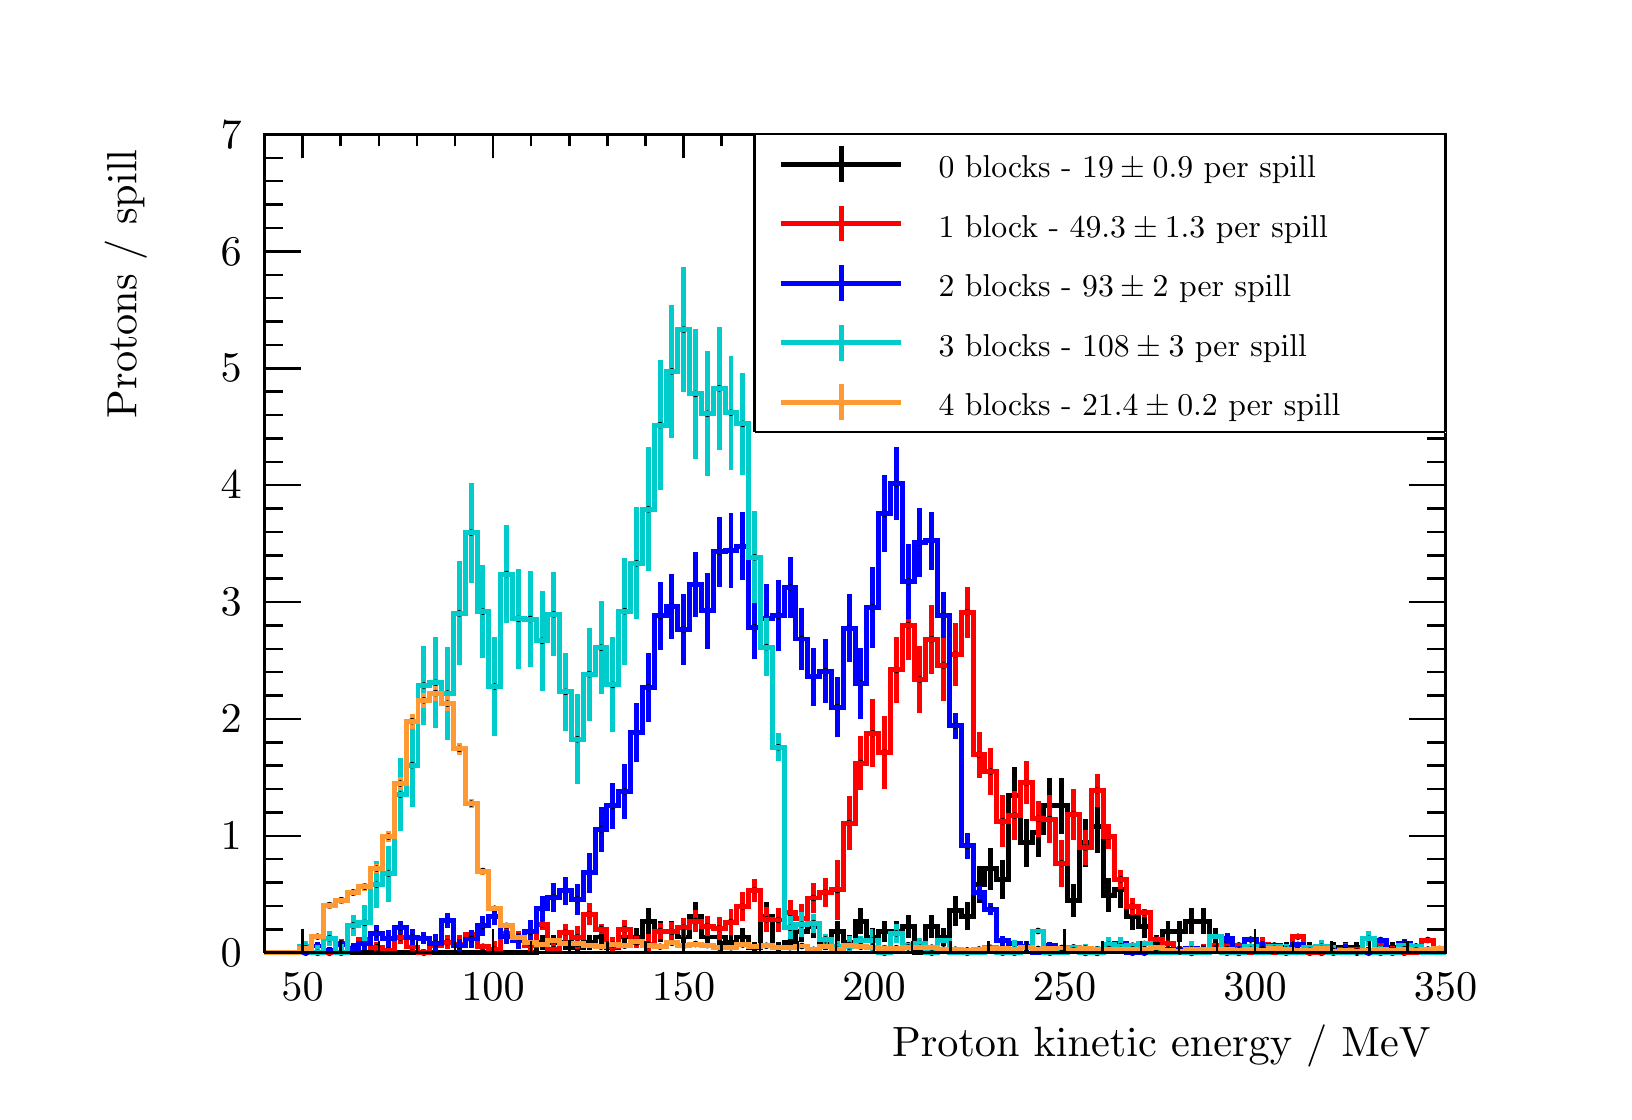
\begin{tikzpicture}
\pgfdeclareplotmark{cross} {
\pgfpathmoveto{\pgfpoint{-0.3\pgfplotmarksize}{\pgfplotmarksize}}
\pgfpathlineto{\pgfpoint{+0.3\pgfplotmarksize}{\pgfplotmarksize}}
\pgfpathlineto{\pgfpoint{+0.3\pgfplotmarksize}{0.3\pgfplotmarksize}}
\pgfpathlineto{\pgfpoint{+1\pgfplotmarksize}{0.3\pgfplotmarksize}}
\pgfpathlineto{\pgfpoint{+1\pgfplotmarksize}{-0.3\pgfplotmarksize}}
\pgfpathlineto{\pgfpoint{+0.3\pgfplotmarksize}{-0.3\pgfplotmarksize}}
\pgfpathlineto{\pgfpoint{+0.3\pgfplotmarksize}{-1.\pgfplotmarksize}}
\pgfpathlineto{\pgfpoint{-0.3\pgfplotmarksize}{-1.\pgfplotmarksize}}
\pgfpathlineto{\pgfpoint{-0.3\pgfplotmarksize}{-0.3\pgfplotmarksize}}
\pgfpathlineto{\pgfpoint{-1.\pgfplotmarksize}{-0.3\pgfplotmarksize}}
\pgfpathlineto{\pgfpoint{-1.\pgfplotmarksize}{0.3\pgfplotmarksize}}
\pgfpathlineto{\pgfpoint{-0.3\pgfplotmarksize}{0.3\pgfplotmarksize}}
\pgfpathclose
\pgfusepathqstroke
}
\pgfdeclareplotmark{cross*} {
\pgfpathmoveto{\pgfpoint{-0.3\pgfplotmarksize}{\pgfplotmarksize}}
\pgfpathlineto{\pgfpoint{+0.3\pgfplotmarksize}{\pgfplotmarksize}}
\pgfpathlineto{\pgfpoint{+0.3\pgfplotmarksize}{0.3\pgfplotmarksize}}
\pgfpathlineto{\pgfpoint{+1\pgfplotmarksize}{0.3\pgfplotmarksize}}
\pgfpathlineto{\pgfpoint{+1\pgfplotmarksize}{-0.3\pgfplotmarksize}}
\pgfpathlineto{\pgfpoint{+0.3\pgfplotmarksize}{-0.3\pgfplotmarksize}}
\pgfpathlineto{\pgfpoint{+0.3\pgfplotmarksize}{-1.\pgfplotmarksize}}
\pgfpathlineto{\pgfpoint{-0.3\pgfplotmarksize}{-1.\pgfplotmarksize}}
\pgfpathlineto{\pgfpoint{-0.3\pgfplotmarksize}{-0.3\pgfplotmarksize}}
\pgfpathlineto{\pgfpoint{-1.\pgfplotmarksize}{-0.3\pgfplotmarksize}}
\pgfpathlineto{\pgfpoint{-1.\pgfplotmarksize}{0.3\pgfplotmarksize}}
\pgfpathlineto{\pgfpoint{-0.3\pgfplotmarksize}{0.3\pgfplotmarksize}}
\pgfpathclose
\pgfusepathqfillstroke
}
\pgfdeclareplotmark{newstar} {
\pgfpathmoveto{\pgfqpoint{0pt}{\pgfplotmarksize}}
\pgfpathlineto{\pgfqpointpolar{44}{0.5\pgfplotmarksize}}
\pgfpathlineto{\pgfqpointpolar{18}{\pgfplotmarksize}}
\pgfpathlineto{\pgfqpointpolar{-20}{0.5\pgfplotmarksize}}
\pgfpathlineto{\pgfqpointpolar{-54}{\pgfplotmarksize}}
\pgfpathlineto{\pgfqpointpolar{-90}{0.5\pgfplotmarksize}}
\pgfpathlineto{\pgfqpointpolar{234}{\pgfplotmarksize}}
\pgfpathlineto{\pgfqpointpolar{198}{0.5\pgfplotmarksize}}
\pgfpathlineto{\pgfqpointpolar{162}{\pgfplotmarksize}}
\pgfpathlineto{\pgfqpointpolar{134}{0.5\pgfplotmarksize}}
\pgfpathclose
\pgfusepathqstroke
}
\pgfdeclareplotmark{newstar*} {
\pgfpathmoveto{\pgfqpoint{0pt}{\pgfplotmarksize}}
\pgfpathlineto{\pgfqpointpolar{44}{0.5\pgfplotmarksize}}
\pgfpathlineto{\pgfqpointpolar{18}{\pgfplotmarksize}}
\pgfpathlineto{\pgfqpointpolar{-20}{0.5\pgfplotmarksize}}
\pgfpathlineto{\pgfqpointpolar{-54}{\pgfplotmarksize}}
\pgfpathlineto{\pgfqpointpolar{-90}{0.5\pgfplotmarksize}}
\pgfpathlineto{\pgfqpointpolar{234}{\pgfplotmarksize}}
\pgfpathlineto{\pgfqpointpolar{198}{0.5\pgfplotmarksize}}
\pgfpathlineto{\pgfqpointpolar{162}{\pgfplotmarksize}}
\pgfpathlineto{\pgfqpointpolar{134}{0.5\pgfplotmarksize}}
\pgfpathclose
\pgfusepathqfillstroke
}
\definecolor{c}{rgb}{1,1,1};
\draw [color=c, fill=c] (0,0) rectangle (20,13.4957);
\draw [color=c, fill=c] (3,1.75444) rectangle (18,12.1461);
\definecolor{c}{rgb}{0,0,0};
\draw [c,line width=0.9] (3,1.75444) -- (3,12.1461) -- (18,12.1461) -- (18,1.75444) -- (3,1.75444);
\definecolor{c}{rgb}{1,1,1};
\draw [color=c, fill=c] (3,1.75444) rectangle (18,12.1461);
\definecolor{c}{rgb}{0,0,0};
\draw [c,line width=0.9] (3,1.75444) -- (3,12.1461) -- (18,12.1461) -- (18,1.75444) -- (3,1.75444);
\draw [c,line width=0.9] (3,1.75444) -- (3.15,1.75444) -- (3.15,1.75444) -- (3.3,1.75444) -- (3.3,1.75444) -- (3.45,1.75444) -- (3.45,1.75444) -- (3.6,1.75444) -- (3.6,1.75444) -- (3.75,1.75444) -- (3.75,1.75444) -- (3.9,1.75444) -- (3.9,1.75444) --
 (4.05,1.75444) -- (4.05,1.75444) -- (4.2,1.75444) -- (4.2,1.75444) -- (4.35,1.75444) -- (4.35,1.75444) -- (4.5,1.75444) -- (4.5,1.75444) -- (4.65,1.75444) -- (4.65,1.75444) -- (4.8,1.75444) -- (4.8,1.75444) -- (4.95,1.75444) -- (4.95,1.75444) --
 (5.1,1.75444) -- (5.1,1.75444) -- (5.25,1.75444) -- (5.25,1.75444) -- (5.4,1.75444) -- (5.4,1.75444) -- (5.55,1.75444) -- (5.55,1.75444) -- (5.7,1.75444) -- (5.7,1.75444) -- (5.85,1.75444) -- (5.85,1.75444) -- (6,1.75444) -- (6,1.75444) --
 (6.15,1.75444) -- (6.15,1.75444) -- (6.3,1.75444) -- (6.3,1.75444) -- (6.45,1.75444) -- (6.45,1.75444) -- (6.6,1.75444) -- (6.6,1.75444) -- (6.75,1.75444) -- (6.75,1.75444) -- (6.9,1.75444) -- (6.9,1.75444) -- (7.05,1.75444) -- (7.05,1.75444) --
 (7.2,1.75444) -- (7.2,1.75444) -- (7.35,1.75444) -- (7.35,1.75444) -- (7.5,1.75444) -- (7.5,1.75444) -- (7.65,1.75444) -- (7.65,1.75444) -- (7.8,1.75444) -- (7.8,1.75444) -- (7.95,1.75444) -- (7.95,1.75444) -- (8.1,1.75444) -- (8.1,1.75444) --
 (8.25,1.75444) -- (8.25,1.75444) -- (8.4,1.75444) -- (8.4,1.75444) -- (8.55,1.75444) -- (8.55,1.75444) -- (8.7,1.75444) -- (8.7,1.75444) -- (8.85,1.75444) -- (8.85,1.75444) -- (9,1.75444) -- (9,1.75444) -- (9.15,1.75444) -- (9.15,1.75444) --
 (9.3,1.75444) -- (9.3,1.75444) -- (9.45,1.75444) -- (9.45,1.75444) -- (9.6,1.75444) -- (9.6,1.75444) -- (9.75,1.75444) -- (9.75,1.75444) -- (9.9,1.75444) -- (9.9,1.75444) -- (10.05,1.75444) -- (10.05,1.75444) -- (10.2,1.75444) -- (10.2,1.75444) --
 (10.35,1.75444) -- (10.35,1.75444) -- (10.5,1.75444) -- (10.5,1.75444) -- (10.65,1.75444) -- (10.65,1.75444) -- (10.8,1.75444) -- (10.8,1.75444) -- (10.95,1.75444) -- (10.95,1.75444) -- (11.1,1.75444) -- (11.1,1.75444) -- (11.25,1.75444) --
 (11.25,1.75444) -- (11.4,1.75444) -- (11.4,1.75444) -- (11.55,1.75444) -- (11.55,1.75444) -- (11.7,1.75444) -- (11.7,1.75444) -- (11.85,1.75444) -- (11.85,1.75444) -- (12,1.75444) -- (12,1.75444) -- (12.15,1.75444) -- (12.15,1.75444) --
 (12.3,1.75444) -- (12.3,1.75444) -- (12.45,1.75444) -- (12.45,1.75444) -- (12.6,1.75444) -- (12.6,1.75444) -- (12.75,1.75444) -- (12.75,1.75444) -- (12.9,1.75444) -- (12.9,1.75444) -- (13.05,1.75444) -- (13.05,1.75444) -- (13.2,1.75444) --
 (13.2,1.75444) -- (13.35,1.75444) -- (13.35,1.75444) -- (13.5,1.75444) -- (13.5,1.75444) -- (13.65,1.75444) -- (13.65,1.75444) -- (13.8,1.75444) -- (13.8,1.75444) -- (13.95,1.75444) -- (13.95,1.75444) -- (14.1,1.75444) -- (14.1,1.75444) --
 (14.25,1.75444) -- (14.25,1.75444) -- (14.4,1.75444) -- (14.4,1.75444) -- (14.55,1.75444) -- (14.55,1.75444) -- (14.7,1.75444) -- (14.7,1.75444) -- (14.85,1.75444) -- (14.85,1.75444) -- (15,1.75444) -- (15,1.75444) -- (15.15,1.75444) --
 (15.15,1.75444) -- (15.3,1.75444) -- (15.3,1.75444) -- (15.45,1.75444) -- (15.45,1.75444) -- (15.6,1.75444) -- (15.6,1.75444) -- (15.75,1.75444) -- (15.75,1.75444) -- (15.9,1.75444) -- (15.9,1.75444) -- (16.05,1.75444) -- (16.05,1.75444) --
 (16.2,1.75444) -- (16.2,1.75444) -- (16.35,1.75444) -- (16.35,1.75444) -- (16.5,1.75444) -- (16.5,1.75444) -- (16.65,1.75444) -- (16.65,1.75444) -- (16.8,1.75444) -- (16.8,1.75444) -- (16.95,1.75444) -- (16.95,1.75444) -- (17.1,1.75444) --
 (17.1,1.75444) -- (17.25,1.75444) -- (17.25,1.75444) -- (17.4,1.75444) -- (17.4,1.75444) -- (17.55,1.75444) -- (17.55,1.75444) -- (17.7,1.75444) -- (17.7,1.75444) -- (17.85,1.75444) -- (17.85,1.75444) -- (18,1.75444);
\draw [c,line width=0.9] (3,1.75444) -- (18,1.75444);
\draw [c,line width=0.9] (3.48387,2.05809) -- (3.48387,1.75444);
\draw [c,line width=0.9] (3.96774,1.90627) -- (3.96774,1.75444);
\draw [c,line width=0.9] (4.45161,1.90627) -- (4.45161,1.75444);
\draw [c,line width=0.9] (4.93548,1.90627) -- (4.93548,1.75444);
\draw [c,line width=0.9] (5.41935,1.90627) -- (5.41935,1.75444);
\draw [c,line width=0.9] (5.90323,2.05809) -- (5.90323,1.75444);
\draw [c,line width=0.9] (6.3871,1.90627) -- (6.3871,1.75444);
\draw [c,line width=0.9] (6.87097,1.90627) -- (6.87097,1.75444);
\draw [c,line width=0.9] (7.35484,1.90627) -- (7.35484,1.75444);
\draw [c,line width=0.9] (7.83871,1.90627) -- (7.83871,1.75444);
\draw [c,line width=0.9] (8.32258,2.05809) -- (8.32258,1.75444);
\draw [c,line width=0.9] (8.80645,1.90627) -- (8.80645,1.75444);
\draw [c,line width=0.9] (9.29032,1.90627) -- (9.29032,1.75444);
\draw [c,line width=0.9] (9.77419,1.90627) -- (9.77419,1.75444);
\draw [c,line width=0.9] (10.2581,1.90627) -- (10.2581,1.75444);
\draw [c,line width=0.9] (10.7419,2.05809) -- (10.7419,1.75444);
\draw [c,line width=0.9] (11.2258,1.90627) -- (11.2258,1.75444);
\draw [c,line width=0.9] (11.7097,1.90627) -- (11.7097,1.75444);
\draw [c,line width=0.9] (12.1935,1.90627) -- (12.1935,1.75444);
\draw [c,line width=0.9] (12.6774,1.90627) -- (12.6774,1.75444);
\draw [c,line width=0.9] (13.1613,2.05809) -- (13.1613,1.75444);
\draw [c,line width=0.9] (13.6452,1.90627) -- (13.6452,1.75444);
\draw [c,line width=0.9] (14.129,1.90627) -- (14.129,1.75444);
\draw [c,line width=0.9] (14.6129,1.90627) -- (14.6129,1.75444);
\draw [c,line width=0.9] (15.0968,1.90627) -- (15.0968,1.75444);
\draw [c,line width=0.9] (15.5806,2.05809) -- (15.5806,1.75444);
\draw [c,line width=0.9] (16.0645,1.90627) -- (16.0645,1.75444);
\draw [c,line width=0.9] (16.5484,1.90627) -- (16.5484,1.75444);
\draw [c,line width=0.9] (17.0323,1.90627) -- (17.0323,1.75444);
\draw [c,line width=0.9] (17.5161,1.90627) -- (17.5161,1.75444);
\draw [c,line width=0.9] (18,2.05809) -- (18,1.75444);
\draw [c,line width=0.9] (3.48387,2.05809) -- (3.48387,1.75444);
\draw [c,line width=0.9] (18,2.05809) -- (18,1.75444);
\draw [anchor=base] (3.48387,1.14713) node[scale=1.52731, color=c, rotate=0]{50};
\draw [anchor=base] (5.90323,1.14713) node[scale=1.52731, color=c, rotate=0]{100};
\draw [anchor=base] (8.32258,1.14713) node[scale=1.52731, color=c, rotate=0]{150};
\draw [anchor=base] (10.7419,1.14713) node[scale=1.52731, color=c, rotate=0]{200};
\draw [anchor=base] (13.1613,1.14713) node[scale=1.52731, color=c, rotate=0]{250};
\draw [anchor=base] (15.5806,1.14713) node[scale=1.52731, color=c, rotate=0]{300};
\draw [anchor=base] (18,1.14713) node[scale=1.52731, color=c, rotate=0]{350};
\draw [anchor= east] (18,0.566819) node[scale=1.52731, color=c, rotate=0]{ Proton kinetic energy / MeV};
\draw [c,line width=0.9] (3,12.1461) -- (18,12.1461);
\draw [c,line width=0.9] (3.48387,11.8425) -- (3.48387,12.1461);
\draw [c,line width=0.9] (3.96774,11.9943) -- (3.96774,12.1461);
\draw [c,line width=0.9] (4.45161,11.9943) -- (4.45161,12.1461);
\draw [c,line width=0.9] (4.93548,11.9943) -- (4.93548,12.1461);
\draw [c,line width=0.9] (5.41935,11.9943) -- (5.41935,12.1461);
\draw [c,line width=0.9] (5.90323,11.8425) -- (5.90323,12.1461);
\draw [c,line width=0.9] (6.3871,11.9943) -- (6.3871,12.1461);
\draw [c,line width=0.9] (6.87097,11.9943) -- (6.87097,12.1461);
\draw [c,line width=0.9] (7.35484,11.9943) -- (7.35484,12.1461);
\draw [c,line width=0.9] (7.83871,11.9943) -- (7.83871,12.1461);
\draw [c,line width=0.9] (8.32258,11.8425) -- (8.32258,12.1461);
\draw [c,line width=0.9] (8.80645,11.9943) -- (8.80645,12.1461);
\draw [c,line width=0.9] (9.29032,11.9943) -- (9.29032,12.1461);
\draw [c,line width=0.9] (9.77419,11.9943) -- (9.77419,12.1461);
\draw [c,line width=0.9] (10.2581,11.9943) -- (10.2581,12.1461);
\draw [c,line width=0.9] (10.7419,11.8425) -- (10.7419,12.1461);
\draw [c,line width=0.9] (11.2258,11.9943) -- (11.2258,12.1461);
\draw [c,line width=0.9] (11.7097,11.9943) -- (11.7097,12.1461);
\draw [c,line width=0.9] (12.1935,11.9943) -- (12.1935,12.1461);
\draw [c,line width=0.9] (12.6774,11.9943) -- (12.6774,12.1461);
\draw [c,line width=0.9] (13.1613,11.8425) -- (13.1613,12.1461);
\draw [c,line width=0.9] (13.6452,11.9943) -- (13.6452,12.1461);
\draw [c,line width=0.9] (14.129,11.9943) -- (14.129,12.1461);
\draw [c,line width=0.9] (14.6129,11.9943) -- (14.6129,12.1461);
\draw [c,line width=0.9] (15.0968,11.9943) -- (15.0968,12.1461);
\draw [c,line width=0.9] (15.5806,11.8425) -- (15.5806,12.1461);
\draw [c,line width=0.9] (16.0645,11.9943) -- (16.0645,12.1461);
\draw [c,line width=0.9] (16.5484,11.9943) -- (16.5484,12.1461);
\draw [c,line width=0.9] (17.0323,11.9943) -- (17.0323,12.1461);
\draw [c,line width=0.9] (17.5161,11.9943) -- (17.5161,12.1461);
\draw [c,line width=0.9] (18,11.8425) -- (18,12.1461);
\draw [c,line width=0.9] (3.48387,11.8425) -- (3.48387,12.1461);
\draw [c,line width=0.9] (18,11.8425) -- (18,12.1461);
\draw [c,line width=0.9] (3,1.75444) -- (3,12.1461);
\draw [c,line width=0.9] (3.462,1.75444) -- (3,1.75444);
\draw [c,line width=0.9] (3.231,2.05135) -- (3,2.05135);
\draw [c,line width=0.9] (3.231,2.34825) -- (3,2.34825);
\draw [c,line width=0.9] (3.231,2.64516) -- (3,2.64516);
\draw [c,line width=0.9] (3.231,2.94206) -- (3,2.94206);
\draw [c,line width=0.9] (3.462,3.23897) -- (3,3.23897);
\draw [c,line width=0.9] (3.231,3.53587) -- (3,3.53587);
\draw [c,line width=0.9] (3.231,3.83278) -- (3,3.83278);
\draw [c,line width=0.9] (3.231,4.12968) -- (3,4.12968);
\draw [c,line width=0.9] (3.231,4.42659) -- (3,4.42659);
\draw [c,line width=0.9] (3.462,4.7235) -- (3,4.7235);
\draw [c,line width=0.9] (3.231,5.0204) -- (3,5.0204);
\draw [c,line width=0.9] (3.231,5.31731) -- (3,5.31731);
\draw [c,line width=0.9] (3.231,5.61421) -- (3,5.61421);
\draw [c,line width=0.9] (3.231,5.91112) -- (3,5.91112);
\draw [c,line width=0.9] (3.462,6.20802) -- (3,6.20802);
\draw [c,line width=0.9] (3.231,6.50493) -- (3,6.50493);
\draw [c,line width=0.9] (3.231,6.80183) -- (3,6.80183);
\draw [c,line width=0.9] (3.231,7.09874) -- (3,7.09874);
\draw [c,line width=0.9] (3.231,7.39564) -- (3,7.39564);
\draw [c,line width=0.9] (3.462,7.69255) -- (3,7.69255);
\draw [c,line width=0.9] (3.231,7.98946) -- (3,7.98946);
\draw [c,line width=0.9] (3.231,8.28636) -- (3,8.28636);
\draw [c,line width=0.9] (3.231,8.58327) -- (3,8.58327);
\draw [c,line width=0.9] (3.231,8.88017) -- (3,8.88017);
\draw [c,line width=0.9] (3.462,9.17708) -- (3,9.17708);
\draw [c,line width=0.9] (3.231,9.47398) -- (3,9.47398);
\draw [c,line width=0.9] (3.231,9.77089) -- (3,9.77089);
\draw [c,line width=0.9] (3.231,10.0678) -- (3,10.0678);
\draw [c,line width=0.9] (3.231,10.3647) -- (3,10.3647);
\draw [c,line width=0.9] (3.462,10.6616) -- (3,10.6616);
\draw [c,line width=0.9] (3.231,10.9585) -- (3,10.9585);
\draw [c,line width=0.9] (3.231,11.2554) -- (3,11.2554);
\draw [c,line width=0.9] (3.231,11.5523) -- (3,11.5523);
\draw [c,line width=0.9] (3.231,11.8492) -- (3,11.8492);
\draw [c,line width=0.9] (3.462,12.1461) -- (3,12.1461);
\draw [anchor= east] (2.9,1.75444) node[scale=1.52731, color=c, rotate=0]{0};
\draw [anchor= east] (2.9,3.23897) node[scale=1.52731, color=c, rotate=0]{1};
\draw [anchor= east] (2.9,4.7235) node[scale=1.52731, color=c, rotate=0]{2};
\draw [anchor= east] (2.9,6.20802) node[scale=1.52731, color=c, rotate=0]{3};
\draw [anchor= east] (2.9,7.69255) node[scale=1.52731, color=c, rotate=0]{4};
\draw [anchor= east] (2.9,9.17708) node[scale=1.52731, color=c, rotate=0]{5};
\draw [anchor= east] (2.9,10.6616) node[scale=1.52731, color=c, rotate=0]{6};
\draw [anchor= east] (2.9,12.1461) node[scale=1.52731, color=c, rotate=0]{7};
\draw [anchor= east] (1.24,12.1461) node[scale=1.52731, color=c, rotate=90]{ Protons / spill};
\draw [c,line width=0.9] (18,1.75444) -- (18,12.1461);
\draw [c,line width=0.9] (17.538,1.75444) -- (18,1.75444);
\draw [c,line width=0.9] (17.769,2.05135) -- (18,2.05135);
\draw [c,line width=0.9] (17.769,2.34825) -- (18,2.34825);
\draw [c,line width=0.9] (17.769,2.64516) -- (18,2.64516);
\draw [c,line width=0.9] (17.769,2.94206) -- (18,2.94206);
\draw [c,line width=0.9] (17.538,3.23897) -- (18,3.23897);
\draw [c,line width=0.9] (17.769,3.53587) -- (18,3.53587);
\draw [c,line width=0.9] (17.769,3.83278) -- (18,3.83278);
\draw [c,line width=0.9] (17.769,4.12968) -- (18,4.12968);
\draw [c,line width=0.9] (17.769,4.42659) -- (18,4.42659);
\draw [c,line width=0.9] (17.538,4.7235) -- (18,4.7235);
\draw [c,line width=0.9] (17.769,5.0204) -- (18,5.0204);
\draw [c,line width=0.9] (17.769,5.31731) -- (18,5.31731);
\draw [c,line width=0.9] (17.769,5.61421) -- (18,5.61421);
\draw [c,line width=0.9] (17.769,5.91112) -- (18,5.91112);
\draw [c,line width=0.9] (17.538,6.20802) -- (18,6.20802);
\draw [c,line width=0.9] (17.769,6.50493) -- (18,6.50493);
\draw [c,line width=0.9] (17.769,6.80183) -- (18,6.80183);
\draw [c,line width=0.9] (17.769,7.09874) -- (18,7.09874);
\draw [c,line width=0.9] (17.769,7.39564) -- (18,7.39564);
\draw [c,line width=0.9] (17.538,7.69255) -- (18,7.69255);
\draw [c,line width=0.9] (17.769,7.98946) -- (18,7.98946);
\draw [c,line width=0.9] (17.769,8.28636) -- (18,8.28636);
\draw [c,line width=0.9] (17.769,8.58327) -- (18,8.58327);
\draw [c,line width=0.9] (17.769,8.88017) -- (18,8.88017);
\draw [c,line width=0.9] (17.538,9.17708) -- (18,9.17708);
\draw [c,line width=0.9] (17.769,9.47398) -- (18,9.47398);
\draw [c,line width=0.9] (17.769,9.77089) -- (18,9.77089);
\draw [c,line width=0.9] (17.769,10.0678) -- (18,10.0678);
\draw [c,line width=0.9] (17.769,10.3647) -- (18,10.3647);
\draw [c,line width=0.9] (17.538,10.6616) -- (18,10.6616);
\draw [c,line width=0.9] (17.769,10.9585) -- (18,10.9585);
\draw [c,line width=0.9] (17.769,11.2554) -- (18,11.2554);
\draw [c,line width=0.9] (17.769,11.5523) -- (18,11.5523);
\draw [c,line width=0.9] (17.769,11.8492) -- (18,11.8492);
\draw [c,line width=0.9] (17.538,12.1461) -- (18,12.1461);
\draw [c,line width=1.8] (6.525,1.79346) -- (6.525,1.88768);
\draw [c,line width=1.8] (6.525,1.88768) -- (6.525,1.9819);
\foreach \P in {(6.525,1.88768)}{\draw[mark options={color=c,fill=c},mark size=2.402402pt,mark=*,mark size=1pt] plot coordinates {\P};}
\draw [c,line width=1.8] (6.675,1.79346) -- (6.675,1.88768);
\draw [c,line width=1.8] (6.675,1.88768) -- (6.675,1.9819);
\foreach \P in {(6.675,1.88768)}{\draw[mark options={color=c,fill=c},mark size=2.402402pt,mark=*,mark size=1pt] plot coordinates {\P};}
\draw [c,line width=1.8] (6.825,1.79346) -- (6.825,1.88768);
\draw [c,line width=1.8] (6.825,1.88768) -- (6.825,1.9819);
\foreach \P in {(6.825,1.88768)}{\draw[mark options={color=c,fill=c},mark size=2.402402pt,mark=*,mark size=1pt] plot coordinates {\P};}
\draw [c,line width=1.8] (6.975,1.75444) -- (6.975,1.82106);
\draw [c,line width=1.8] (6.975,1.82106) -- (6.975,1.88769);
\foreach \P in {(6.975,1.82106)}{\draw[mark options={color=c,fill=c},mark size=2.402402pt,mark=*,mark size=1pt] plot coordinates {\P};}
\draw [c,line width=1.8] (7.125,1.79346) -- (7.125,1.88768);
\draw [c,line width=1.8] (7.125,1.88768) -- (7.125,1.9819);
\foreach \P in {(7.125,1.88768)}{\draw[mark options={color=c,fill=c},mark size=2.402402pt,mark=*,mark size=1pt] plot coordinates {\P};}
\draw [c,line width=1.8] (7.275,1.83891) -- (7.275,1.9543);
\draw [c,line width=1.8] (7.275,1.9543) -- (7.275,2.0697);
\foreach \P in {(7.275,1.9543)}{\draw[mark options={color=c,fill=c},mark size=2.402402pt,mark=*,mark size=1pt] plot coordinates {\P};}
\draw [c,line width=1.8] (7.425,1.75444) -- (7.425,1.82106);
\draw [c,line width=1.8] (7.425,1.82106) -- (7.425,1.88769);
\foreach \P in {(7.425,1.82106)}{\draw[mark options={color=c,fill=c},mark size=2.402402pt,mark=*,mark size=1pt] plot coordinates {\P};}
\draw [c,line width=1.8] (7.575,1.83891) -- (7.575,1.9543);
\draw [c,line width=1.8] (7.575,1.9543) -- (7.575,2.0697);
\foreach \P in {(7.575,1.9543)}{\draw[mark options={color=c,fill=c},mark size=2.402402pt,mark=*,mark size=1pt] plot coordinates {\P};}
\draw [c,line width=1.8] (7.725,1.83891) -- (7.725,1.9543);
\draw [c,line width=1.8] (7.725,1.9543) -- (7.725,2.0697);
\foreach \P in {(7.725,1.9543)}{\draw[mark options={color=c,fill=c},mark size=2.402402pt,mark=*,mark size=1pt] plot coordinates {\P};}
\draw [c,line width=1.8] (7.875,1.99097) -- (7.875,2.15417);
\draw [c,line width=1.8] (7.875,2.15417) -- (7.875,2.31736);
\foreach \P in {(7.875,2.15417)}{\draw[mark options={color=c,fill=c},mark size=2.402402pt,mark=*,mark size=1pt] plot coordinates {\P};}
\draw [c,line width=1.8] (8.025,1.88767) -- (8.025,2.02092);
\draw [c,line width=1.8] (8.025,2.02092) -- (8.025,2.15417);
\foreach \P in {(8.025,2.02092)}{\draw[mark options={color=c,fill=c},mark size=2.402402pt,mark=*,mark size=1pt] plot coordinates {\P};}
\draw [c,line width=1.8] (8.175,1.88767) -- (8.175,2.02092);
\draw [c,line width=1.8] (8.175,2.02092) -- (8.175,2.15417);
\foreach \P in {(8.175,2.02092)}{\draw[mark options={color=c,fill=c},mark size=2.402402pt,mark=*,mark size=1pt] plot coordinates {\P};}
\draw [c,line width=1.8] (8.325,1.83891) -- (8.325,1.9543);
\draw [c,line width=1.8] (8.325,1.9543) -- (8.325,2.0697);
\foreach \P in {(8.325,1.9543)}{\draw[mark options={color=c,fill=c},mark size=2.402402pt,mark=*,mark size=1pt] plot coordinates {\P};}
\draw [c,line width=1.8] (8.475,2.04451) -- (8.475,2.22079);
\draw [c,line width=1.8] (8.475,2.22079) -- (8.475,2.39706);
\foreach \P in {(8.475,2.22079)}{\draw[mark options={color=c,fill=c},mark size=2.402402pt,mark=*,mark size=1pt] plot coordinates {\P};}
\draw [c,line width=1.8] (8.625,1.83891) -- (8.625,1.9543);
\draw [c,line width=1.8] (8.625,1.9543) -- (8.625,2.0697);
\foreach \P in {(8.625,1.9543)}{\draw[mark options={color=c,fill=c},mark size=2.402402pt,mark=*,mark size=1pt] plot coordinates {\P};}
\draw [c,line width=1.8] (8.775,1.83891) -- (8.775,1.9543);
\draw [c,line width=1.8] (8.775,1.9543) -- (8.775,2.0697);
\foreach \P in {(8.775,1.9543)}{\draw[mark options={color=c,fill=c},mark size=2.402402pt,mark=*,mark size=1pt] plot coordinates {\P};}
\draw [c,line width=1.8] (8.925,1.79346) -- (8.925,1.88768);
\draw [c,line width=1.8] (8.925,1.88768) -- (8.925,1.9819);
\foreach \P in {(8.925,1.88768)}{\draw[mark options={color=c,fill=c},mark size=2.402402pt,mark=*,mark size=1pt] plot coordinates {\P};}
\draw [c,line width=1.8] (9.075,1.83891) -- (9.075,1.9543);
\draw [c,line width=1.8] (9.075,1.9543) -- (9.075,2.0697);
\foreach \P in {(9.075,1.9543)}{\draw[mark options={color=c,fill=c},mark size=2.402402pt,mark=*,mark size=1pt] plot coordinates {\P};}
\draw [c,line width=1.8] (9.225,1.75444) -- (9.225,1.82106);
\draw [c,line width=1.8] (9.225,1.82106) -- (9.225,1.88769);
\foreach \P in {(9.225,1.82106)}{\draw[mark options={color=c,fill=c},mark size=2.402402pt,mark=*,mark size=1pt] plot coordinates {\P};}
\draw [c,line width=1.8] (9.375,2.04451) -- (9.375,2.22079);
\draw [c,line width=1.8] (9.375,2.22079) -- (9.375,2.39706);
\foreach \P in {(9.375,2.22079)}{\draw[mark options={color=c,fill=c},mark size=2.402402pt,mark=*,mark size=1pt] plot coordinates {\P};}
\draw [c,line width=1.8] (9.525,1.75444) -- (9.525,1.82106);
\draw [c,line width=1.8] (9.525,1.82106) -- (9.525,1.88769);
\foreach \P in {(9.525,1.82106)}{\draw[mark options={color=c,fill=c},mark size=2.402402pt,mark=*,mark size=1pt] plot coordinates {\P};}
\draw [c,line width=1.8] (9.675,1.79346) -- (9.675,1.88768);
\draw [c,line width=1.8] (9.675,1.88768) -- (9.675,1.9819);
\foreach \P in {(9.675,1.88768)}{\draw[mark options={color=c,fill=c},mark size=2.402402pt,mark=*,mark size=1pt] plot coordinates {\P};}
\draw [c,line width=1.8] (9.825,1.88767) -- (9.825,2.02092);
\draw [c,line width=1.8] (9.825,2.02092) -- (9.825,2.15417);
\foreach \P in {(9.825,2.02092)}{\draw[mark options={color=c,fill=c},mark size=2.402402pt,mark=*,mark size=1pt] plot coordinates {\P};}
\draw [c,line width=1.8] (9.975,1.93857) -- (9.975,2.08755);
\draw [c,line width=1.8] (9.975,2.08755) -- (9.975,2.23652);
\foreach \P in {(9.975,2.08755)}{\draw[mark options={color=c,fill=c},mark size=2.402402pt,mark=*,mark size=1pt] plot coordinates {\P};}
\draw [c,line width=1.8] (10.125,1.79346) -- (10.125,1.88768);
\draw [c,line width=1.8] (10.125,1.88768) -- (10.125,1.9819);
\foreach \P in {(10.125,1.88768)}{\draw[mark options={color=c,fill=c},mark size=2.402402pt,mark=*,mark size=1pt] plot coordinates {\P};}
\draw [c,line width=1.8] (10.275,1.88767) -- (10.275,2.02092);
\draw [c,line width=1.8] (10.275,2.02092) -- (10.275,2.15417);
\foreach \P in {(10.275,2.02092)}{\draw[mark options={color=c,fill=c},mark size=2.402402pt,mark=*,mark size=1pt] plot coordinates {\P};}
\draw [c,line width=1.8] (10.425,1.79346) -- (10.425,1.88768);
\draw [c,line width=1.8] (10.425,1.88768) -- (10.425,1.9819);
\foreach \P in {(10.425,1.88768)}{\draw[mark options={color=c,fill=c},mark size=2.402402pt,mark=*,mark size=1pt] plot coordinates {\P};}
\draw [c,line width=1.8] (10.575,1.99097) -- (10.575,2.15417);
\draw [c,line width=1.8] (10.575,2.15417) -- (10.575,2.31736);
\foreach \P in {(10.575,2.15417)}{\draw[mark options={color=c,fill=c},mark size=2.402402pt,mark=*,mark size=1pt] plot coordinates {\P};}
\draw [c,line width=1.8] (10.725,1.83891) -- (10.725,1.9543);
\draw [c,line width=1.8] (10.725,1.9543) -- (10.725,2.0697);
\foreach \P in {(10.725,1.9543)}{\draw[mark options={color=c,fill=c},mark size=2.402402pt,mark=*,mark size=1pt] plot coordinates {\P};}
\draw [c,line width=1.8] (10.875,1.88767) -- (10.875,2.02092);
\draw [c,line width=1.8] (10.875,2.02092) -- (10.875,2.15417);
\foreach \P in {(10.875,2.02092)}{\draw[mark options={color=c,fill=c},mark size=2.402402pt,mark=*,mark size=1pt] plot coordinates {\P};}
\draw [c,line width=1.8] (11.025,1.88767) -- (11.025,2.02092);
\draw [c,line width=1.8] (11.025,2.02092) -- (11.025,2.15417);
\foreach \P in {(11.025,2.02092)}{\draw[mark options={color=c,fill=c},mark size=2.402402pt,mark=*,mark size=1pt] plot coordinates {\P};}
\draw [c,line width=1.8] (11.175,1.93857) -- (11.175,2.08755);
\draw [c,line width=1.8] (11.175,2.08755) -- (11.175,2.23652);
\foreach \P in {(11.175,2.08755)}{\draw[mark options={color=c,fill=c},mark size=2.402402pt,mark=*,mark size=1pt] plot coordinates {\P};}
\draw [c,line width=1.8] (11.475,1.93857) -- (11.475,2.08755);
\draw [c,line width=1.8] (11.475,2.08755) -- (11.475,2.23652);
\foreach \P in {(11.475,2.08755)}{\draw[mark options={color=c,fill=c},mark size=2.402402pt,mark=*,mark size=1pt] plot coordinates {\P};}
\draw [c,line width=1.8] (11.625,1.83891) -- (11.625,1.9543);
\draw [c,line width=1.8] (11.625,1.9543) -- (11.625,2.0697);
\foreach \P in {(11.625,1.9543)}{\draw[mark options={color=c,fill=c},mark size=2.402402pt,mark=*,mark size=1pt] plot coordinates {\P};}
\draw [c,line width=1.8] (11.775,2.09896) -- (11.775,2.28741);
\draw [c,line width=1.8] (11.775,2.28741) -- (11.775,2.47585);
\foreach \P in {(11.775,2.28741)}{\draw[mark options={color=c,fill=c},mark size=2.402402pt,mark=*,mark size=1pt] plot coordinates {\P};}
\draw [c,line width=1.8] (11.925,2.04451) -- (11.925,2.22079);
\draw [c,line width=1.8] (11.925,2.22079) -- (11.925,2.39706);
\foreach \P in {(11.925,2.22079)}{\draw[mark options={color=c,fill=c},mark size=2.402402pt,mark=*,mark size=1pt] plot coordinates {\P};}
\draw [c,line width=1.8] (12.075,2.38029) -- (12.075,2.62051);
\draw [c,line width=1.8] (12.075,2.62051) -- (12.075,2.86073);
\foreach \P in {(12.075,2.62051)}{\draw[mark options={color=c,fill=c},mark size=2.402402pt,mark=*,mark size=1pt] plot coordinates {\P};}
\draw [c,line width=1.8] (12.225,2.55387) -- (12.225,2.82037);
\draw [c,line width=1.8] (12.225,2.82037) -- (12.225,3.08687);
\foreach \P in {(12.225,2.82037)}{\draw[mark options={color=c,fill=c},mark size=2.402402pt,mark=*,mark size=1pt] plot coordinates {\P};}
\draw [c,line width=1.8] (12.375,2.43784) -- (12.375,2.68713);
\draw [c,line width=1.8] (12.375,2.68713) -- (12.375,2.93642);
\foreach \P in {(12.375,2.68713)}{\draw[mark options={color=c,fill=c},mark size=2.402402pt,mark=*,mark size=1pt] plot coordinates {\P};}
\draw [c,line width=1.8] (12.525,3.38815) -- (12.525,3.75307);
\draw [c,line width=1.8] (12.525,3.75307) -- (12.525,4.11799);
\foreach \P in {(12.525,3.75307)}{\draw[mark options={color=c,fill=c},mark size=2.402402pt,mark=*,mark size=1pt] plot coordinates {\P};}
\draw [c,line width=1.8] (12.675,2.84816) -- (12.675,3.15348);
\draw [c,line width=1.8] (12.675,3.15348) -- (12.675,3.45879);
\foreach \P in {(12.675,3.15348)}{\draw[mark options={color=c,fill=c},mark size=2.402402pt,mark=*,mark size=1pt] plot coordinates {\P};}
\draw [c,line width=1.8] (12.825,2.9672) -- (12.825,3.28672);
\draw [c,line width=1.8] (12.825,3.28672) -- (12.825,3.60624);
\foreach \P in {(12.825,3.28672)}{\draw[mark options={color=c,fill=c},mark size=2.402402pt,mark=*,mark size=1pt] plot coordinates {\P};}
\draw [c,line width=1.8] (12.975,3.26728) -- (12.975,3.61982);
\draw [c,line width=1.8] (12.975,3.61982) -- (12.975,3.97237);
\foreach \P in {(12.975,3.61982)}{\draw[mark options={color=c,fill=c},mark size=2.402402pt,mark=*,mark size=1pt] plot coordinates {\P};}
\draw [c,line width=1.8] (13.125,3.26728) -- (13.125,3.61982);
\draw [c,line width=1.8] (13.125,3.61982) -- (13.125,3.97237);
\foreach \P in {(13.125,3.61982)}{\draw[mark options={color=c,fill=c},mark size=2.402402pt,mark=*,mark size=1pt] plot coordinates {\P};}
\draw [c,line width=1.8] (13.275,2.20996) -- (13.275,2.42065);
\draw [c,line width=1.8] (13.275,2.42065) -- (13.275,2.63134);
\foreach \P in {(13.275,2.42065)}{\draw[mark options={color=c,fill=c},mark size=2.402402pt,mark=*,mark size=1pt] plot coordinates {\P};}
\draw [c,line width=1.8] (13.425,2.84816) -- (13.425,3.15348);
\draw [c,line width=1.8] (13.425,3.15348) -- (13.425,3.45879);
\foreach \P in {(13.425,3.15348)}{\draw[mark options={color=c,fill=c},mark size=2.402402pt,mark=*,mark size=1pt] plot coordinates {\P};}
\draw [c,line width=1.8] (13.575,3.02695) -- (13.575,3.35334);
\draw [c,line width=1.8] (13.575,3.35334) -- (13.575,3.67974);
\foreach \P in {(13.575,3.35334)}{\draw[mark options={color=c,fill=c},mark size=2.402402pt,mark=*,mark size=1pt] plot coordinates {\P};}
\draw [c,line width=1.8] (13.725,2.2663) -- (13.725,2.48727);
\draw [c,line width=1.8] (13.725,2.48727) -- (13.725,2.70824);
\foreach \P in {(13.725,2.48727)}{\draw[mark options={color=c,fill=c},mark size=2.402402pt,mark=*,mark size=1pt] plot coordinates {\P};}
\draw [c,line width=1.8] (13.875,2.3231) -- (13.875,2.55389);
\draw [c,line width=1.8] (13.875,2.55389) -- (13.875,2.78469);
\foreach \P in {(13.875,2.55389)}{\draw[mark options={color=c,fill=c},mark size=2.402402pt,mark=*,mark size=1pt] plot coordinates {\P};}
\draw [c,line width=1.8] (14.025,2.04451) -- (14.025,2.22079);
\draw [c,line width=1.8] (14.025,2.22079) -- (14.025,2.39706);
\foreach \P in {(14.025,2.22079)}{\draw[mark options={color=c,fill=c},mark size=2.402402pt,mark=*,mark size=1pt] plot coordinates {\P};}
\draw [c,line width=1.8] (14.175,1.93857) -- (14.175,2.08755);
\draw [c,line width=1.8] (14.175,2.08755) -- (14.175,2.23652);
\foreach \P in {(14.175,2.08755)}{\draw[mark options={color=c,fill=c},mark size=2.402402pt,mark=*,mark size=1pt] plot coordinates {\P};}
\draw [c,line width=1.8] (14.325,1.79346) -- (14.325,1.88768);
\draw [c,line width=1.8] (14.325,1.88768) -- (14.325,1.9819);
\foreach \P in {(14.325,1.88768)}{\draw[mark options={color=c,fill=c},mark size=2.402402pt,mark=*,mark size=1pt] plot coordinates {\P};}
\draw [c,line width=1.8] (14.475,1.88767) -- (14.475,2.02092);
\draw [c,line width=1.8] (14.475,2.02092) -- (14.475,2.15417);
\foreach \P in {(14.475,2.02092)}{\draw[mark options={color=c,fill=c},mark size=2.402402pt,mark=*,mark size=1pt] plot coordinates {\P};}
\draw [c,line width=1.8] (14.625,1.88767) -- (14.625,2.02092);
\draw [c,line width=1.8] (14.625,2.02092) -- (14.625,2.15417);
\foreach \P in {(14.625,2.02092)}{\draw[mark options={color=c,fill=c},mark size=2.402402pt,mark=*,mark size=1pt] plot coordinates {\P};}
\draw [c,line width=1.8] (14.775,1.99097) -- (14.775,2.15417);
\draw [c,line width=1.8] (14.775,2.15417) -- (14.775,2.31736);
\foreach \P in {(14.775,2.15417)}{\draw[mark options={color=c,fill=c},mark size=2.402402pt,mark=*,mark size=1pt] plot coordinates {\P};}
\draw [c,line width=1.8] (14.925,1.99097) -- (14.925,2.15417);
\draw [c,line width=1.8] (14.925,2.15417) -- (14.925,2.31736);
\foreach \P in {(14.925,2.15417)}{\draw[mark options={color=c,fill=c},mark size=2.402402pt,mark=*,mark size=1pt] plot coordinates {\P};}
\draw [c,line width=1.8] (15.075,1.83891) -- (15.075,1.9543);
\draw [c,line width=1.8] (15.075,1.9543) -- (15.075,2.0697);
\foreach \P in {(15.075,1.9543)}{\draw[mark options={color=c,fill=c},mark size=2.402402pt,mark=*,mark size=1pt] plot coordinates {\P};}
\draw [c,line width=1.8] (15.225,1.79346) -- (15.225,1.88768);
\draw [c,line width=1.8] (15.225,1.88768) -- (15.225,1.9819);
\foreach \P in {(15.225,1.88768)}{\draw[mark options={color=c,fill=c},mark size=2.402402pt,mark=*,mark size=1pt] plot coordinates {\P};}
\draw [c,line width=1.8] (15.975,1.75444) -- (15.975,1.82106);
\draw [c,line width=1.8] (15.975,1.82106) -- (15.975,1.88769);
\foreach \P in {(15.975,1.82106)}{\draw[mark options={color=c,fill=c},mark size=2.402402pt,mark=*,mark size=1pt] plot coordinates {\P};}
\draw [c,line width=1.8] (16.275,1.75444) -- (16.275,1.82106);
\draw [c,line width=1.8] (16.275,1.82106) -- (16.275,1.88769);
\foreach \P in {(16.275,1.82106)}{\draw[mark options={color=c,fill=c},mark size=2.402402pt,mark=*,mark size=1pt] plot coordinates {\P};}
\draw [c,line width=1.8] (16.575,1.75444) -- (16.575,1.82106);
\draw [c,line width=1.8] (16.575,1.82106) -- (16.575,1.88769);
\foreach \P in {(16.575,1.82106)}{\draw[mark options={color=c,fill=c},mark size=2.402402pt,mark=*,mark size=1pt] plot coordinates {\P};}
\draw [c,line width=1.8] (16.725,1.75444) -- (16.725,1.82106);
\draw [c,line width=1.8] (16.725,1.82106) -- (16.725,1.88769);
\foreach \P in {(16.725,1.82106)}{\draw[mark options={color=c,fill=c},mark size=2.402402pt,mark=*,mark size=1pt] plot coordinates {\P};}
\draw [c,line width=1.8] (16.875,1.75444) -- (16.875,1.82106);
\draw [c,line width=1.8] (16.875,1.82106) -- (16.875,1.88769);
\foreach \P in {(16.875,1.82106)}{\draw[mark options={color=c,fill=c},mark size=2.402402pt,mark=*,mark size=1pt] plot coordinates {\P};}
\draw [c,line width=1.8] (17.175,1.75444) -- (17.175,1.82106);
\draw [c,line width=1.8] (17.175,1.82106) -- (17.175,1.88769);
\foreach \P in {(17.175,1.82106)}{\draw[mark options={color=c,fill=c},mark size=2.402402pt,mark=*,mark size=1pt] plot coordinates {\P};}
\draw [c,line width=1.8] (17.325,1.75444) -- (17.325,1.82106);
\draw [c,line width=1.8] (17.325,1.82106) -- (17.325,1.88769);
\foreach \P in {(17.325,1.82106)}{\draw[mark options={color=c,fill=c},mark size=2.402402pt,mark=*,mark size=1pt] plot coordinates {\P};}
\draw [c,line width=1.8] (3,1.75444) -- (3.15,1.75444) -- (3.15,1.75444) -- (3.3,1.75444) -- (3.3,1.75444) -- (3.45,1.75444) -- (3.45,1.75444) -- (3.6,1.75444) -- (3.6,1.75444) -- (3.75,1.75444) -- (3.75,1.75444) -- (3.9,1.75444) -- (3.9,1.75444) --
 (4.05,1.75444) -- (4.05,1.75444) -- (4.2,1.75444) -- (4.2,1.75444) -- (4.35,1.75444) -- (4.35,1.75444) -- (4.5,1.75444) -- (4.5,1.75444) -- (4.65,1.75444) -- (4.65,1.75444) -- (4.8,1.75444) -- (4.8,1.75444) -- (4.95,1.75444) -- (4.95,1.75444) --
 (5.1,1.75444) -- (5.1,1.75444) -- (5.25,1.75444) -- (5.25,1.75444) -- (5.4,1.75444) -- (5.4,1.75444) -- (5.55,1.75444) -- (5.55,1.75444) -- (5.7,1.75444) -- (5.7,1.75444) -- (5.85,1.75444) -- (5.85,1.75444) -- (6,1.75444) -- (6,1.75444) --
 (6.15,1.75444) -- (6.15,1.75444) -- (6.3,1.75444) -- (6.3,1.75444) -- (6.45,1.75444) -- (6.45,1.88768) -- (6.6,1.88768) -- (6.6,1.88768) -- (6.75,1.88768) -- (6.75,1.88768) -- (6.9,1.88768) -- (6.9,1.82106) -- (7.05,1.82106) -- (7.05,1.88768) --
 (7.2,1.88768) -- (7.2,1.9543) -- (7.35,1.9543) -- (7.35,1.82106) -- (7.5,1.82106) -- (7.5,1.9543) -- (7.65,1.9543) -- (7.65,1.9543) -- (7.8,1.9543) -- (7.8,2.15417) -- (7.95,2.15417) -- (7.95,2.02092) -- (8.1,2.02092) -- (8.1,2.02092) --
 (8.25,2.02092) -- (8.25,1.9543) -- (8.4,1.9543) -- (8.4,2.22079) -- (8.55,2.22079) -- (8.55,1.9543) -- (8.7,1.9543) -- (8.7,1.9543) -- (8.85,1.9543) -- (8.85,1.88768) -- (9,1.88768) -- (9,1.9543) -- (9.15,1.9543) -- (9.15,1.82106) -- (9.3,1.82106)
 -- (9.3,2.22079) -- (9.45,2.22079) -- (9.45,1.82106) -- (9.6,1.82106) -- (9.6,1.88768) -- (9.75,1.88768) -- (9.75,2.02092) -- (9.9,2.02092) -- (9.9,2.08755) -- (10.05,2.08755) -- (10.05,1.88768) -- (10.2,1.88768) -- (10.2,2.02092) -- (10.35,2.02092)
 -- (10.35,1.88768) -- (10.5,1.88768) -- (10.5,2.15417) -- (10.65,2.15417) -- (10.65,1.9543) -- (10.8,1.9543) -- (10.8,2.02092) -- (10.95,2.02092) -- (10.95,2.02092) -- (11.1,2.02092) -- (11.1,2.08755) -- (11.25,2.08755) -- (11.25,1.75444) --
 (11.4,1.75444) -- (11.4,2.08755) -- (11.55,2.08755) -- (11.55,1.9543) -- (11.7,1.9543) -- (11.7,2.28741) -- (11.85,2.28741) -- (11.85,2.22079) -- (12,2.22079) -- (12,2.62051) -- (12.15,2.62051) -- (12.15,2.82037) -- (12.3,2.82037) -- (12.3,2.68713)
 -- (12.45,2.68713) -- (12.45,3.75307) -- (12.6,3.75307) -- (12.6,3.15348) -- (12.75,3.15348) -- (12.75,3.28672) -- (12.9,3.28672) -- (12.9,3.61982) -- (13.05,3.61982) -- (13.05,3.61982) -- (13.2,3.61982) -- (13.2,2.42065) -- (13.35,2.42065) --
 (13.35,3.15348) -- (13.5,3.15348) -- (13.5,3.35334) -- (13.65,3.35334) -- (13.65,2.48727) -- (13.8,2.48727) -- (13.8,2.55389) -- (13.95,2.55389) -- (13.95,2.22079) -- (14.1,2.22079) -- (14.1,2.08755) -- (14.25,2.08755) -- (14.25,1.88768) --
 (14.4,1.88768) -- (14.4,2.02092) -- (14.55,2.02092) -- (14.55,2.02092) -- (14.7,2.02092) -- (14.7,2.15417) -- (14.85,2.15417) -- (14.85,2.15417) -- (15,2.15417) -- (15,1.9543) -- (15.15,1.9543) -- (15.15,1.88768) -- (15.3,1.88768) -- (15.3,1.75444)
 -- (15.45,1.75444) -- (15.45,1.75444) -- (15.6,1.75444) -- (15.6,1.75444) -- (15.75,1.75444) -- (15.75,1.75444) -- (15.9,1.75444) -- (15.9,1.82106) -- (16.05,1.82106) -- (16.05,1.75444) -- (16.2,1.75444) -- (16.2,1.82106) -- (16.35,1.82106) --
 (16.35,1.75444) -- (16.5,1.75444) -- (16.5,1.82106) -- (16.65,1.82106) -- (16.65,1.82106) -- (16.8,1.82106) -- (16.8,1.82106) -- (16.95,1.82106) -- (16.95,1.75444) -- (17.1,1.75444) -- (17.1,1.82106) -- (17.25,1.82106) -- (17.25,1.82106) --
 (17.4,1.82106) -- (17.4,1.75444) -- (17.55,1.75444) -- (17.55,1.75444) -- (17.7,1.75444) -- (17.7,1.75444) -- (17.85,1.75444) -- (17.85,1.75444) -- (18,1.75444);
\definecolor{c}{rgb}{1,0,0};
\draw [c,line width=1.8] (3.825,1.75444) -- (3.825,1.79985);
\definecolor{c}{rgb}{0,0,0};
\foreach \P in {(3.825,1.75444)}{\draw[mark options={color=c,fill=c},mark size=2.402402pt,mark=*,mark size=1pt] plot coordinates {\P};}
\definecolor{c}{rgb}{1,0,0};
\draw [c,line width=1.8] (3.975,1.82031) -- (3.975,1.87354);
\draw [c,line width=1.8] (3.975,1.87354) -- (3.975,1.92677);
\definecolor{c}{rgb}{0,0,0};
\foreach \P in {(3.975,1.87354)}{\draw[mark options={color=c,fill=c},mark size=2.402402pt,mark=*,mark size=1pt] plot coordinates {\P};}
\definecolor{c}{rgb}{1,0,0};
\draw [c,line width=1.8] (4.125,1.75444) -- (4.125,1.78432);
\draw [c,line width=1.8] (4.125,1.78432) -- (4.125,1.84824);
\definecolor{c}{rgb}{0,0,0};
\foreach \P in {(4.125,1.78432)}{\draw[mark options={color=c,fill=c},mark size=2.402402pt,mark=*,mark size=1pt] plot coordinates {\P};}
\definecolor{c}{rgb}{1,0,0};
\draw [c,line width=1.8] (4.275,1.84049) -- (4.275,1.92236);
\draw [c,line width=1.8] (4.275,1.92236) -- (4.275,2.00423);
\definecolor{c}{rgb}{0,0,0};
\foreach \P in {(4.275,1.92236)}{\draw[mark options={color=c,fill=c},mark size=2.402402pt,mark=*,mark size=1pt] plot coordinates {\P};}
\definecolor{c}{rgb}{1,0,0};
\draw [c,line width=1.8] (4.425,1.76305) -- (4.425,1.82446);
\draw [c,line width=1.8] (4.425,1.82446) -- (4.425,1.88588);
\definecolor{c}{rgb}{0,0,0};
\foreach \P in {(4.425,1.82446)}{\draw[mark options={color=c,fill=c},mark size=2.402402pt,mark=*,mark size=1pt] plot coordinates {\P};}
\definecolor{c}{rgb}{1,0,0};
\draw [c,line width=1.8] (4.575,1.75444) -- (4.575,1.7886);
\draw [c,line width=1.8] (4.575,1.7886) -- (4.575,1.84649);
\definecolor{c}{rgb}{0,0,0};
\foreach \P in {(4.575,1.7886)}{\draw[mark options={color=c,fill=c},mark size=2.402402pt,mark=*,mark size=1pt] plot coordinates {\P};}
\definecolor{c}{rgb}{1,0,0};
\draw [c,line width=1.8] (4.725,1.86769) -- (4.725,1.94838);
\draw [c,line width=1.8] (4.725,1.94838) -- (4.725,2.02906);
\definecolor{c}{rgb}{0,0,0};
\foreach \P in {(4.725,1.94838)}{\draw[mark options={color=c,fill=c},mark size=2.402402pt,mark=*,mark size=1pt] plot coordinates {\P};}
\definecolor{c}{rgb}{1,0,0};
\draw [c,line width=1.8] (4.875,1.77485) -- (4.875,1.82738);
\draw [c,line width=1.8] (4.875,1.82738) -- (4.875,1.87992);
\definecolor{c}{rgb}{0,0,0};
\foreach \P in {(4.875,1.82738)}{\draw[mark options={color=c,fill=c},mark size=2.402402pt,mark=*,mark size=1pt] plot coordinates {\P};}
\definecolor{c}{rgb}{1,0,0};
\draw [c,line width=1.8] (5.025,1.75444) -- (5.025,1.80022);
\definecolor{c}{rgb}{0,0,0};
\foreach \P in {(5.025,1.75444)}{\draw[mark options={color=c,fill=c},mark size=2.402402pt,mark=*,mark size=1pt] plot coordinates {\P};}
\definecolor{c}{rgb}{1,0,0};
\draw [c,line width=1.8] (5.175,1.79445) -- (5.175,1.85065);
\draw [c,line width=1.8] (5.175,1.85065) -- (5.175,1.90686);
\definecolor{c}{rgb}{0,0,0};
\foreach \P in {(5.175,1.85065)}{\draw[mark options={color=c,fill=c},mark size=2.402402pt,mark=*,mark size=1pt] plot coordinates {\P};}
\definecolor{c}{rgb}{1,0,0};
\draw [c,line width=1.8] (5.325,1.79732) -- (5.325,1.88864);
\draw [c,line width=1.8] (5.325,1.88864) -- (5.325,1.97996);
\definecolor{c}{rgb}{0,0,0};
\foreach \P in {(5.325,1.88864)}{\draw[mark options={color=c,fill=c},mark size=2.402402pt,mark=*,mark size=1pt] plot coordinates {\P};}
\definecolor{c}{rgb}{1,0,0};
\draw [c,line width=1.8] (5.475,1.75444) -- (5.475,1.86486);
\draw [c,line width=1.8] (5.475,1.86486) -- (5.475,1.98375);
\definecolor{c}{rgb}{0,0,0};
\foreach \P in {(5.475,1.86486)}{\draw[mark options={color=c,fill=c},mark size=2.402402pt,mark=*,mark size=1pt] plot coordinates {\P};}
\definecolor{c}{rgb}{1,0,0};
\draw [c,line width=1.8] (5.625,1.92581) -- (5.625,1.98113);
\draw [c,line width=1.8] (5.625,1.98113) -- (5.625,2.03645);
\definecolor{c}{rgb}{0,0,0};
\foreach \P in {(5.625,1.98113)}{\draw[mark options={color=c,fill=c},mark size=2.402402pt,mark=*,mark size=1pt] plot coordinates {\P};}
\definecolor{c}{rgb}{1,0,0};
\draw [c,line width=1.8] (5.775,1.79303) -- (5.775,1.8316);
\draw [c,line width=1.8] (5.775,1.8316) -- (5.775,1.87017);
\definecolor{c}{rgb}{0,0,0};
\foreach \P in {(5.775,1.8316)}{\draw[mark options={color=c,fill=c},mark size=2.402402pt,mark=*,mark size=1pt] plot coordinates {\P};}
\definecolor{c}{rgb}{1,0,0};
\draw [c,line width=1.8] (5.925,1.75444) -- (5.925,1.79263);
\draw [c,line width=1.8] (5.925,1.79263) -- (5.925,1.90444);
\definecolor{c}{rgb}{0,0,0};
\foreach \P in {(5.925,1.79263)}{\draw[mark options={color=c,fill=c},mark size=2.402402pt,mark=*,mark size=1pt] plot coordinates {\P};}
\definecolor{c}{rgb}{1,0,0};
\draw [c,line width=1.8] (6.075,1.91601) -- (6.075,1.99395);
\draw [c,line width=1.8] (6.075,1.99395) -- (6.075,2.07188);
\definecolor{c}{rgb}{0,0,0};
\foreach \P in {(6.075,1.99395)}{\draw[mark options={color=c,fill=c},mark size=2.402402pt,mark=*,mark size=1pt] plot coordinates {\P};}
\definecolor{c}{rgb}{1,0,0};
\draw [c,line width=1.8] (6.225,1.81659) -- (6.225,1.9212);
\draw [c,line width=1.8] (6.225,1.9212) -- (6.225,2.02582);
\definecolor{c}{rgb}{0,0,0};
\foreach \P in {(6.225,1.9212)}{\draw[mark options={color=c,fill=c},mark size=2.402402pt,mark=*,mark size=1pt] plot coordinates {\P};}
\definecolor{c}{rgb}{1,0,0};
\draw [c,line width=1.8] (6.375,1.75444) -- (6.375,1.8522);
\draw [c,line width=1.8] (6.375,1.8522) -- (6.375,1.96921);
\definecolor{c}{rgb}{0,0,0};
\foreach \P in {(6.375,1.8522)}{\draw[mark options={color=c,fill=c},mark size=2.402402pt,mark=*,mark size=1pt] plot coordinates {\P};}
\definecolor{c}{rgb}{1,0,0};
\draw [c,line width=1.8] (6.525,2.0386) -- (6.525,2.11242);
\draw [c,line width=1.8] (6.525,2.11242) -- (6.525,2.18624);
\definecolor{c}{rgb}{0,0,0};
\foreach \P in {(6.525,2.11242)}{\draw[mark options={color=c,fill=c},mark size=2.402402pt,mark=*,mark size=1pt] plot coordinates {\P};}
\definecolor{c}{rgb}{1,0,0};
\draw [c,line width=1.8] (6.675,1.75444) -- (6.675,1.80018);
\draw [c,line width=1.8] (6.675,1.80018) -- (6.675,1.9077);
\definecolor{c}{rgb}{0,0,0};
\foreach \P in {(6.675,1.80018)}{\draw[mark options={color=c,fill=c},mark size=2.402402pt,mark=*,mark size=1pt] plot coordinates {\P};}
\definecolor{c}{rgb}{1,0,0};
\draw [c,line width=1.8] (6.825,1.90405) -- (6.825,2.01285);
\draw [c,line width=1.8] (6.825,2.01285) -- (6.825,2.12165);
\definecolor{c}{rgb}{0,0,0};
\foreach \P in {(6.825,2.01285)}{\draw[mark options={color=c,fill=c},mark size=2.402402pt,mark=*,mark size=1pt] plot coordinates {\P};}
\definecolor{c}{rgb}{1,0,0};
\draw [c,line width=1.8] (6.975,1.80573) -- (6.975,1.95023);
\draw [c,line width=1.8] (6.975,1.95023) -- (6.975,2.09473);
\definecolor{c}{rgb}{0,0,0};
\foreach \P in {(6.975,1.95023)}{\draw[mark options={color=c,fill=c},mark size=2.402402pt,mark=*,mark size=1pt] plot coordinates {\P};}
\definecolor{c}{rgb}{1,0,0};
\draw [c,line width=1.8] (7.125,2.10413) -- (7.125,2.24205);
\draw [c,line width=1.8] (7.125,2.24205) -- (7.125,2.37996);
\definecolor{c}{rgb}{0,0,0};
\foreach \P in {(7.125,2.24205)}{\draw[mark options={color=c,fill=c},mark size=2.402402pt,mark=*,mark size=1pt] plot coordinates {\P};}
\definecolor{c}{rgb}{1,0,0};
\draw [c,line width=1.8] (7.275,1.99515) -- (7.275,2.0545);
\draw [c,line width=1.8] (7.275,2.0545) -- (7.275,2.11385);
\definecolor{c}{rgb}{0,0,0};
\foreach \P in {(7.275,2.0545)}{\draw[mark options={color=c,fill=c},mark size=2.402402pt,mark=*,mark size=1pt] plot coordinates {\P};}
\definecolor{c}{rgb}{1,0,0};
\draw [c,line width=1.8] (7.425,1.75444) -- (7.425,1.83853);
\draw [c,line width=1.8] (7.425,1.83853) -- (7.425,1.95516);
\definecolor{c}{rgb}{0,0,0};
\foreach \P in {(7.425,1.83853)}{\draw[mark options={color=c,fill=c},mark size=2.402402pt,mark=*,mark size=1pt] plot coordinates {\P};}
\definecolor{c}{rgb}{1,0,0};
\draw [c,line width=1.8] (7.575,1.94182) -- (7.575,2.05429);
\draw [c,line width=1.8] (7.575,2.05429) -- (7.575,2.16677);
\definecolor{c}{rgb}{0,0,0};
\foreach \P in {(7.575,2.05429)}{\draw[mark options={color=c,fill=c},mark size=2.402402pt,mark=*,mark size=1pt] plot coordinates {\P};}
\definecolor{c}{rgb}{1,0,0};
\draw [c,line width=1.8] (7.725,1.81197) -- (7.725,1.88799);
\draw [c,line width=1.8] (7.725,1.88799) -- (7.725,1.964);
\definecolor{c}{rgb}{0,0,0};
\foreach \P in {(7.725,1.88799)}{\draw[mark options={color=c,fill=c},mark size=2.402402pt,mark=*,mark size=1pt] plot coordinates {\P};}
\definecolor{c}{rgb}{1,0,0};
\draw [c,line width=1.8] (7.875,1.75444) -- (7.875,1.8591);
\draw [c,line width=1.8] (7.875,1.8591) -- (7.875,1.98619);
\definecolor{c}{rgb}{0,0,0};
\foreach \P in {(7.875,1.8591)}{\draw[mark options={color=c,fill=c},mark size=2.402402pt,mark=*,mark size=1pt] plot coordinates {\P};}
\definecolor{c}{rgb}{1,0,0};
\draw [c,line width=1.8] (8.025,1.92937) -- (8.025,2.02968);
\draw [c,line width=1.8] (8.025,2.02968) -- (8.025,2.12998);
\definecolor{c}{rgb}{0,0,0};
\foreach \P in {(8.025,2.02968)}{\draw[mark options={color=c,fill=c},mark size=2.402402pt,mark=*,mark size=1pt] plot coordinates {\P};}
\definecolor{c}{rgb}{1,0,0};
\draw [c,line width=1.8] (8.175,1.88898) -- (8.175,2.01959);
\draw [c,line width=1.8] (8.175,2.01959) -- (8.175,2.1502);
\definecolor{c}{rgb}{0,0,0};
\foreach \P in {(8.175,2.01959)}{\draw[mark options={color=c,fill=c},mark size=2.402402pt,mark=*,mark size=1pt] plot coordinates {\P};}
\definecolor{c}{rgb}{1,0,0};
\draw [c,line width=1.8] (8.325,1.95244) -- (8.325,2.07264);
\draw [c,line width=1.8] (8.325,2.07264) -- (8.325,2.19284);
\definecolor{c}{rgb}{0,0,0};
\foreach \P in {(8.325,2.07264)}{\draw[mark options={color=c,fill=c},mark size=2.402402pt,mark=*,mark size=1pt] plot coordinates {\P};}
\definecolor{c}{rgb}{1,0,0};
\draw [c,line width=1.8] (8.475,2.01691) -- (8.475,2.15521);
\draw [c,line width=1.8] (8.475,2.15521) -- (8.475,2.29351);
\definecolor{c}{rgb}{0,0,0};
\foreach \P in {(8.475,2.15521)}{\draw[mark options={color=c,fill=c},mark size=2.402402pt,mark=*,mark size=1pt] plot coordinates {\P};}
\definecolor{c}{rgb}{1,0,0};
\draw [c,line width=1.8] (8.625,1.96136) -- (8.625,2.09105);
\draw [c,line width=1.8] (8.625,2.09105) -- (8.625,2.22075);
\definecolor{c}{rgb}{0,0,0};
\foreach \P in {(8.625,2.09105)}{\draw[mark options={color=c,fill=c},mark size=2.402402pt,mark=*,mark size=1pt] plot coordinates {\P};}
\definecolor{c}{rgb}{1,0,0};
\draw [c,line width=1.8] (8.775,1.91738) -- (8.775,2.06458);
\draw [c,line width=1.8] (8.775,2.06458) -- (8.775,2.21178);
\definecolor{c}{rgb}{0,0,0};
\foreach \P in {(8.775,2.06458)}{\draw[mark options={color=c,fill=c},mark size=2.402402pt,mark=*,mark size=1pt] plot coordinates {\P};}
\definecolor{c}{rgb}{1,0,0};
\draw [c,line width=1.8] (8.925,1.9762) -- (8.925,2.14436);
\draw [c,line width=1.8] (8.925,2.14436) -- (8.925,2.31252);
\definecolor{c}{rgb}{0,0,0};
\foreach \P in {(8.925,2.14436)}{\draw[mark options={color=c,fill=c},mark size=2.402402pt,mark=*,mark size=1pt] plot coordinates {\P};}
\definecolor{c}{rgb}{1,0,0};
\draw [c,line width=1.8] (9.075,2.15402) -- (9.075,2.3384);
\draw [c,line width=1.8] (9.075,2.3384) -- (9.075,2.52278);
\definecolor{c}{rgb}{0,0,0};
\foreach \P in {(9.075,2.3384)}{\draw[mark options={color=c,fill=c},mark size=2.402402pt,mark=*,mark size=1pt] plot coordinates {\P};}
\definecolor{c}{rgb}{1,0,0};
\draw [c,line width=1.8] (9.225,2.40394) -- (9.225,2.54735);
\draw [c,line width=1.8] (9.225,2.54735) -- (9.225,2.69076);
\definecolor{c}{rgb}{0,0,0};
\foreach \P in {(9.225,2.54735)}{\draw[mark options={color=c,fill=c},mark size=2.402402pt,mark=*,mark size=1pt] plot coordinates {\P};}
\definecolor{c}{rgb}{1,0,0};
\draw [c,line width=1.8] (9.375,2.01903) -- (9.375,2.17879);
\draw [c,line width=1.8] (9.375,2.17879) -- (9.375,2.33856);
\definecolor{c}{rgb}{0,0,0};
\foreach \P in {(9.375,2.17879)}{\draw[mark options={color=c,fill=c},mark size=2.402402pt,mark=*,mark size=1pt] plot coordinates {\P};}
\definecolor{c}{rgb}{1,0,0};
\draw [c,line width=1.8] (9.525,2.01846) -- (9.525,2.17023);
\draw [c,line width=1.8] (9.525,2.17023) -- (9.525,2.322);
\definecolor{c}{rgb}{0,0,0};
\foreach \P in {(9.525,2.17023)}{\draw[mark options={color=c,fill=c},mark size=2.402402pt,mark=*,mark size=1pt] plot coordinates {\P};}
\definecolor{c}{rgb}{1,0,0};
\draw [c,line width=1.8] (9.675,2.10053) -- (9.675,2.26107);
\draw [c,line width=1.8] (9.675,2.26107) -- (9.675,2.42161);
\definecolor{c}{rgb}{0,0,0};
\foreach \P in {(9.675,2.26107)}{\draw[mark options={color=c,fill=c},mark size=2.402402pt,mark=*,mark size=1pt] plot coordinates {\P};}
\definecolor{c}{rgb}{1,0,0};
\draw [c,line width=1.8] (9.825,2.00335) -- (9.825,2.19025);
\draw [c,line width=1.8] (9.825,2.19025) -- (9.825,2.37714);
\definecolor{c}{rgb}{0,0,0};
\foreach \P in {(9.825,2.19025)}{\draw[mark options={color=c,fill=c},mark size=2.402402pt,mark=*,mark size=1pt] plot coordinates {\P};}
\definecolor{c}{rgb}{1,0,0};
\draw [c,line width=1.8] (9.975,2.25756) -- (9.975,2.44966);
\draw [c,line width=1.8] (9.975,2.44966) -- (9.975,2.64175);
\definecolor{c}{rgb}{0,0,0};
\foreach \P in {(9.975,2.44966)}{\draw[mark options={color=c,fill=c},mark size=2.402402pt,mark=*,mark size=1pt] plot coordinates {\P};}
\definecolor{c}{rgb}{1,0,0};
\draw [c,line width=1.8] (10.125,2.33421) -- (10.125,2.52109);
\draw [c,line width=1.8] (10.125,2.52109) -- (10.125,2.70798);
\definecolor{c}{rgb}{0,0,0};
\foreach \P in {(10.125,2.52109)}{\draw[mark options={color=c,fill=c},mark size=2.402402pt,mark=*,mark size=1pt] plot coordinates {\P};}
\definecolor{c}{rgb}{1,0,0};
\draw [c,line width=1.8] (10.275,2.1745) -- (10.275,2.55136);
\draw [c,line width=1.8] (10.275,2.55136) -- (10.275,2.92821);
\definecolor{c}{rgb}{0,0,0};
\foreach \P in {(10.275,2.55136)}{\draw[mark options={color=c,fill=c},mark size=2.402402pt,mark=*,mark size=1pt] plot coordinates {\P};}
\definecolor{c}{rgb}{1,0,0};
\draw [c,line width=1.8] (10.425,3.05873) -- (10.425,3.4014);
\draw [c,line width=1.8] (10.425,3.4014) -- (10.425,3.74407);
\definecolor{c}{rgb}{0,0,0};
\foreach \P in {(10.425,3.4014)}{\draw[mark options={color=c,fill=c},mark size=2.402402pt,mark=*,mark size=1pt] plot coordinates {\P};}
\definecolor{c}{rgb}{1,0,0};
\draw [c,line width=1.8] (10.575,3.8185) -- (10.575,4.16319);
\draw [c,line width=1.8] (10.575,4.16319) -- (10.575,4.50787);
\definecolor{c}{rgb}{0,0,0};
\foreach \P in {(10.575,4.16319)}{\draw[mark options={color=c,fill=c},mark size=2.402402pt,mark=*,mark size=1pt] plot coordinates {\P};}
\definecolor{c}{rgb}{1,0,0};
\draw [c,line width=1.8] (10.725,4.11269) -- (10.725,4.54308);
\draw [c,line width=1.8] (10.725,4.54308) -- (10.725,4.97347);
\definecolor{c}{rgb}{0,0,0};
\foreach \P in {(10.725,4.54308)}{\draw[mark options={color=c,fill=c},mark size=2.402402pt,mark=*,mark size=1pt] plot coordinates {\P};}
\definecolor{c}{rgb}{1,0,0};
\draw [c,line width=1.8] (10.875,3.83694) -- (10.875,4.29911);
\draw [c,line width=1.8] (10.875,4.29911) -- (10.875,4.76128);
\definecolor{c}{rgb}{0,0,0};
\foreach \P in {(10.875,4.29911)}{\draw[mark options={color=c,fill=c},mark size=2.402402pt,mark=*,mark size=1pt] plot coordinates {\P};}
\definecolor{c}{rgb}{1,0,0};
\draw [c,line width=1.8] (11.025,4.92534) -- (11.025,5.34591);
\draw [c,line width=1.8] (11.025,5.34591) -- (11.025,5.76648);
\definecolor{c}{rgb}{0,0,0};
\foreach \P in {(11.025,5.34591)}{\draw[mark options={color=c,fill=c},mark size=2.402402pt,mark=*,mark size=1pt] plot coordinates {\P};}
\definecolor{c}{rgb}{1,0,0};
\draw [c,line width=1.8] (11.175,5.47795) -- (11.175,5.91397);
\draw [c,line width=1.8] (11.175,5.91397) -- (11.175,6.34999);
\definecolor{c}{rgb}{0,0,0};
\foreach \P in {(11.175,5.91397)}{\draw[mark options={color=c,fill=c},mark size=2.402402pt,mark=*,mark size=1pt] plot coordinates {\P};}
\definecolor{c}{rgb}{1,0,0};
\draw [c,line width=1.8] (11.325,4.79742) -- (11.325,5.22384);
\draw [c,line width=1.8] (11.325,5.22384) -- (11.325,5.65025);
\definecolor{c}{rgb}{0,0,0};
\foreach \P in {(11.325,5.22384)}{\draw[mark options={color=c,fill=c},mark size=2.402402pt,mark=*,mark size=1pt] plot coordinates {\P};}
\definecolor{c}{rgb}{1,0,0};
\draw [c,line width=1.8] (11.475,5.30025) -- (11.475,5.73556);
\draw [c,line width=1.8] (11.475,5.73556) -- (11.475,6.17088);
\definecolor{c}{rgb}{0,0,0};
\foreach \P in {(11.475,5.73556)}{\draw[mark options={color=c,fill=c},mark size=2.402402pt,mark=*,mark size=1pt] plot coordinates {\P};}
\definecolor{c}{rgb}{1,0,0};
\draw [c,line width=1.8] (11.625,4.94848) -- (11.625,5.40245);
\draw [c,line width=1.8] (11.625,5.40245) -- (11.625,5.85642);
\definecolor{c}{rgb}{0,0,0};
\foreach \P in {(11.625,5.40245)}{\draw[mark options={color=c,fill=c},mark size=2.402402pt,mark=*,mark size=1pt] plot coordinates {\P};}
\definecolor{c}{rgb}{1,0,0};
\draw [c,line width=1.8] (11.775,5.14316) -- (11.775,5.54172);
\draw [c,line width=1.8] (11.775,5.54172) -- (11.775,5.94028);
\definecolor{c}{rgb}{0,0,0};
\foreach \P in {(11.775,5.54172)}{\draw[mark options={color=c,fill=c},mark size=2.402402pt,mark=*,mark size=1pt] plot coordinates {\P};}
\definecolor{c}{rgb}{1,0,0};
\draw [c,line width=1.8] (11.925,5.75459) -- (11.925,6.07885);
\draw [c,line width=1.8] (11.925,6.07885) -- (11.925,6.40312);
\definecolor{c}{rgb}{0,0,0};
\foreach \P in {(11.925,6.07885)}{\draw[mark options={color=c,fill=c},mark size=2.402402pt,mark=*,mark size=1pt] plot coordinates {\P};}
\definecolor{c}{rgb}{1,0,0};
\draw [c,line width=1.8] (12.075,3.97452) -- (12.075,4.2688);
\draw [c,line width=1.8] (12.075,4.2688) -- (12.075,4.56307);
\definecolor{c}{rgb}{0,0,0};
\foreach \P in {(12.075,4.2688)}{\draw[mark options={color=c,fill=c},mark size=2.402402pt,mark=*,mark size=1pt] plot coordinates {\P};}
\definecolor{c}{rgb}{1,0,0};
\draw [c,line width=1.8] (12.225,3.75334) -- (12.225,4.05549);
\draw [c,line width=1.8] (12.225,4.05549) -- (12.225,4.35764);
\definecolor{c}{rgb}{0,0,0};
\foreach \P in {(12.225,4.05549)}{\draw[mark options={color=c,fill=c},mark size=2.402402pt,mark=*,mark size=1pt] plot coordinates {\P};}
\definecolor{c}{rgb}{1,0,0};
\draw [c,line width=1.8] (12.375,3.09105) -- (12.375,3.42607);
\draw [c,line width=1.8] (12.375,3.42607) -- (12.375,3.76109);
\definecolor{c}{rgb}{0,0,0};
\foreach \P in {(12.375,3.42607)}{\draw[mark options={color=c,fill=c},mark size=2.402402pt,mark=*,mark size=1pt] plot coordinates {\P};}
\definecolor{c}{rgb}{1,0,0};
\draw [c,line width=1.8] (12.525,3.18826) -- (12.525,3.49574);
\draw [c,line width=1.8] (12.525,3.49574) -- (12.525,3.80323);
\definecolor{c}{rgb}{0,0,0};
\foreach \P in {(12.525,3.49574)}{\draw[mark options={color=c,fill=c},mark size=2.402402pt,mark=*,mark size=1pt] plot coordinates {\P};}
\definecolor{c}{rgb}{1,0,0};
\draw [c,line width=1.8] (12.675,3.63922) -- (12.675,3.91191);
\draw [c,line width=1.8] (12.675,3.91191) -- (12.675,4.18461);
\definecolor{c}{rgb}{0,0,0};
\foreach \P in {(12.675,3.91191)}{\draw[mark options={color=c,fill=c},mark size=2.402402pt,mark=*,mark size=1pt] plot coordinates {\P};}
\definecolor{c}{rgb}{1,0,0};
\draw [c,line width=1.8] (12.825,3.22339) -- (12.825,3.45513);
\draw [c,line width=1.8] (12.825,3.45513) -- (12.825,3.68686);
\definecolor{c}{rgb}{0,0,0};
\foreach \P in {(12.825,3.45513)}{\draw[mark options={color=c,fill=c},mark size=2.402402pt,mark=*,mark size=1pt] plot coordinates {\P};}
\definecolor{c}{rgb}{1,0,0};
\draw [c,line width=1.8] (12.975,3.15074) -- (12.975,3.45247);
\draw [c,line width=1.8] (12.975,3.45247) -- (12.975,3.75419);
\definecolor{c}{rgb}{0,0,0};
\foreach \P in {(12.975,3.45247)}{\draw[mark options={color=c,fill=c},mark size=2.402402pt,mark=*,mark size=1pt] plot coordinates {\P};}
\definecolor{c}{rgb}{1,0,0};
\draw [c,line width=1.8] (13.125,2.59027) -- (13.125,2.89061);
\draw [c,line width=1.8] (13.125,2.89061) -- (13.125,3.19095);
\definecolor{c}{rgb}{0,0,0};
\foreach \P in {(13.125,2.89061)}{\draw[mark options={color=c,fill=c},mark size=2.402402pt,mark=*,mark size=1pt] plot coordinates {\P};}
\definecolor{c}{rgb}{1,0,0};
\draw [c,line width=1.8] (13.275,3.18795) -- (13.275,3.51327);
\draw [c,line width=1.8] (13.275,3.51327) -- (13.275,3.83858);
\definecolor{c}{rgb}{0,0,0};
\foreach \P in {(13.275,3.51327)}{\draw[mark options={color=c,fill=c},mark size=2.402402pt,mark=*,mark size=1pt] plot coordinates {\P};}
\definecolor{c}{rgb}{1,0,0};
\draw [c,line width=1.8] (13.425,2.86551) -- (13.425,3.0904);
\draw [c,line width=1.8] (13.425,3.0904) -- (13.425,3.3153);
\definecolor{c}{rgb}{0,0,0};
\foreach \P in {(13.425,3.0904)}{\draw[mark options={color=c,fill=c},mark size=2.402402pt,mark=*,mark size=1pt] plot coordinates {\P};}
\definecolor{c}{rgb}{1,0,0};
\draw [c,line width=1.8] (13.575,3.60544) -- (13.575,3.81592);
\draw [c,line width=1.8] (13.575,3.81592) -- (13.575,4.0264);
\definecolor{c}{rgb}{0,0,0};
\foreach \P in {(13.575,3.81592)}{\draw[mark options={color=c,fill=c},mark size=2.402402pt,mark=*,mark size=1pt] plot coordinates {\P};}
\definecolor{c}{rgb}{1,0,0};
\draw [c,line width=1.8] (13.725,3.06554) -- (13.725,3.22585);
\draw [c,line width=1.8] (13.725,3.22585) -- (13.725,3.38616);
\definecolor{c}{rgb}{0,0,0};
\foreach \P in {(13.725,3.22585)}{\draw[mark options={color=c,fill=c},mark size=2.402402pt,mark=*,mark size=1pt] plot coordinates {\P};}
\definecolor{c}{rgb}{1,0,0};
\draw [c,line width=1.8] (13.875,2.56268) -- (13.875,2.68633);
\draw [c,line width=1.8] (13.875,2.68633) -- (13.875,2.80999);
\definecolor{c}{rgb}{0,0,0};
\foreach \P in {(13.875,2.68633)}{\draw[mark options={color=c,fill=c},mark size=2.402402pt,mark=*,mark size=1pt] plot coordinates {\P};}
\definecolor{c}{rgb}{1,0,0};
\draw [c,line width=1.8] (14.025,2.2278) -- (14.025,2.34009);
\draw [c,line width=1.8] (14.025,2.34009) -- (14.025,2.45238);
\definecolor{c}{rgb}{0,0,0};
\foreach \P in {(14.025,2.34009)}{\draw[mark options={color=c,fill=c},mark size=2.402402pt,mark=*,mark size=1pt] plot coordinates {\P};}
\definecolor{c}{rgb}{1,0,0};
\draw [c,line width=1.8] (14.175,2.21208) -- (14.175,2.26296);
\draw [c,line width=1.8] (14.175,2.26296) -- (14.175,2.31384);
\definecolor{c}{rgb}{0,0,0};
\foreach \P in {(14.175,2.26296)}{\draw[mark options={color=c,fill=c},mark size=2.402402pt,mark=*,mark size=1pt] plot coordinates {\P};}
\definecolor{c}{rgb}{1,0,0};
\draw [c,line width=1.8] (14.325,1.8884) -- (14.325,1.92557);
\draw [c,line width=1.8] (14.325,1.92557) -- (14.325,1.96275);
\definecolor{c}{rgb}{0,0,0};
\foreach \P in {(14.325,1.92557)}{\draw[mark options={color=c,fill=c},mark size=2.402402pt,mark=*,mark size=1pt] plot coordinates {\P};}
\definecolor{c}{rgb}{1,0,0};
\draw [c,line width=1.8] (14.475,1.82903) -- (14.475,1.87113);
\draw [c,line width=1.8] (14.475,1.87113) -- (14.475,1.91323);
\definecolor{c}{rgb}{0,0,0};
\foreach \P in {(14.475,1.87113)}{\draw[mark options={color=c,fill=c},mark size=2.402402pt,mark=*,mark size=1pt] plot coordinates {\P};}
\definecolor{c}{rgb}{1,0,0};
\draw [c,line width=1.8] (14.625,1.75444) -- (14.625,1.79128);
\draw [c,line width=1.8] (14.625,1.79128) -- (14.625,1.83571);
\definecolor{c}{rgb}{0,0,0};
\foreach \P in {(14.625,1.79128)}{\draw[mark options={color=c,fill=c},mark size=2.402402pt,mark=*,mark size=1pt] plot coordinates {\P};}
\definecolor{c}{rgb}{1,0,0};
\draw [c,line width=1.8] (14.775,1.75444) -- (14.775,1.8401);
\definecolor{c}{rgb}{0,0,0};
\foreach \P in {(14.775,1.75444)}{\draw[mark options={color=c,fill=c},mark size=2.402402pt,mark=*,mark size=1pt] plot coordinates {\P};}
\definecolor{c}{rgb}{1,0,0};
\draw [c,line width=1.8] (14.925,1.75444) -- (14.925,1.79603);
\draw [c,line width=1.8] (14.925,1.79603) -- (14.925,1.86349);
\definecolor{c}{rgb}{0,0,0};
\foreach \P in {(14.925,1.79603)}{\draw[mark options={color=c,fill=c},mark size=2.402402pt,mark=*,mark size=1pt] plot coordinates {\P};}
\foreach \P in {(15.075,1.84257)}{\draw[mark options={color=c,fill=c},mark size=2.402402pt,mark=*,mark size=1pt] plot coordinates {\P};}
\definecolor{c}{rgb}{1,0,0};
\draw [c,line width=1.8] (15.225,1.7881) -- (15.225,1.85149);
\draw [c,line width=1.8] (15.225,1.85149) -- (15.225,1.91489);
\definecolor{c}{rgb}{0,0,0};
\foreach \P in {(15.225,1.85149)}{\draw[mark options={color=c,fill=c},mark size=2.402402pt,mark=*,mark size=1pt] plot coordinates {\P};}
\foreach \P in {(15.375,1.84803)}{\draw[mark options={color=c,fill=c},mark size=2.402402pt,mark=*,mark size=1pt] plot coordinates {\P};}
\definecolor{c}{rgb}{1,0,0};
\draw [c,line width=1.8] (15.675,1.76865) -- (15.675,1.86199);
\draw [c,line width=1.8] (15.675,1.86199) -- (15.675,1.95533);
\definecolor{c}{rgb}{0,0,0};
\foreach \P in {(15.675,1.86199)}{\draw[mark options={color=c,fill=c},mark size=2.402402pt,mark=*,mark size=1pt] plot coordinates {\P};}
\foreach \P in {(16.125,1.95761)}{\draw[mark options={color=c,fill=c},mark size=2.402402pt,mark=*,mark size=1pt] plot coordinates {\P};}
\definecolor{c}{rgb}{1,0,0};
\draw [c,line width=1.8] (16.275,1.75444) -- (16.275,1.79368);
\definecolor{c}{rgb}{0,0,0};
\foreach \P in {(16.275,1.75444)}{\draw[mark options={color=c,fill=c},mark size=2.402402pt,mark=*,mark size=1pt] plot coordinates {\P};}
\definecolor{c}{rgb}{1,0,0};
\draw [c,line width=1.8] (16.425,1.75444) -- (16.425,1.79869);
\definecolor{c}{rgb}{0,0,0};
\foreach \P in {(16.425,1.75444)}{\draw[mark options={color=c,fill=c},mark size=2.402402pt,mark=*,mark size=1pt] plot coordinates {\P};}
\definecolor{c}{rgb}{1,0,0};
\draw [c,line width=1.8] (16.725,1.75444) -- (16.725,1.79328);
\draw [c,line width=1.8] (16.725,1.79328) -- (16.725,1.8837);
\definecolor{c}{rgb}{0,0,0};
\foreach \P in {(16.725,1.79328)}{\draw[mark options={color=c,fill=c},mark size=2.402402pt,mark=*,mark size=1pt] plot coordinates {\P};}
\foreach \P in {(16.875,1.79809)}{\draw[mark options={color=c,fill=c},mark size=2.402402pt,mark=*,mark size=1pt] plot coordinates {\P};}
\definecolor{c}{rgb}{1,0,0};
\draw [c,line width=1.8] (17.175,1.83288) -- (17.175,1.87317);
\draw [c,line width=1.8] (17.175,1.87317) -- (17.175,1.91346);
\definecolor{c}{rgb}{0,0,0};
\foreach \P in {(17.175,1.87317)}{\draw[mark options={color=c,fill=c},mark size=2.402402pt,mark=*,mark size=1pt] plot coordinates {\P};}
\definecolor{c}{rgb}{1,0,0};
\draw [c,line width=1.8] (17.325,1.75444) -- (17.325,1.84328);
\definecolor{c}{rgb}{0,0,0};
\foreach \P in {(17.325,1.75444)}{\draw[mark options={color=c,fill=c},mark size=2.402402pt,mark=*,mark size=1pt] plot coordinates {\P};}
\definecolor{c}{rgb}{1,0,0};
\draw [c,line width=1.8] (17.475,1.75444) -- (17.475,1.7909);
\definecolor{c}{rgb}{0,0,0};
\foreach \P in {(17.475,1.75444)}{\draw[mark options={color=c,fill=c},mark size=2.402402pt,mark=*,mark size=1pt] plot coordinates {\P};}
\foreach \P in {(17.775,1.91558)}{\draw[mark options={color=c,fill=c},mark size=2.402402pt,mark=*,mark size=1pt] plot coordinates {\P};}
\foreach \P in {(17.925,1.79059)}{\draw[mark options={color=c,fill=c},mark size=2.402402pt,mark=*,mark size=1pt] plot coordinates {\P};}
\definecolor{c}{rgb}{1,0,0};
\draw [c,line width=1.8] (3,1.75444) -- (3.15,1.75444) -- (3.15,1.75444) -- (3.3,1.75444) -- (3.3,1.75444) -- (3.45,1.75444) -- (3.45,1.75444) -- (3.6,1.75444) -- (3.6,1.75444) -- (3.75,1.75444) -- (3.75,1.75444) -- (3.9,1.75444) -- (3.9,1.87354) --
 (4.05,1.87354) -- (4.05,1.78432) -- (4.2,1.78432) -- (4.2,1.92236) -- (4.35,1.92236) -- (4.35,1.82446) -- (4.5,1.82446) -- (4.5,1.7886) -- (4.65,1.7886) -- (4.65,1.94838) -- (4.8,1.94838) -- (4.8,1.82738) -- (4.95,1.82738) -- (4.95,1.75444) --
 (5.1,1.75444) -- (5.1,1.85065) -- (5.25,1.85065) -- (5.25,1.88864) -- (5.4,1.88864) -- (5.4,1.86486) -- (5.55,1.86486) -- (5.55,1.98113) -- (5.7,1.98113) -- (5.7,1.8316) -- (5.85,1.8316) -- (5.85,1.79263) -- (6,1.79263) -- (6,1.99395) --
 (6.15,1.99395) -- (6.15,1.9212) -- (6.3,1.9212) -- (6.3,1.8522) -- (6.45,1.8522) -- (6.45,2.11242) -- (6.6,2.11242) -- (6.6,1.80018) -- (6.75,1.80018) -- (6.75,2.01285) -- (6.9,2.01285) -- (6.9,1.95023) -- (7.05,1.95023) -- (7.05,2.24205) --
 (7.2,2.24205) -- (7.2,2.0545) -- (7.35,2.0545) -- (7.35,1.83853) -- (7.5,1.83853) -- (7.5,2.05429) -- (7.65,2.05429) -- (7.65,1.88799) -- (7.8,1.88799) -- (7.8,1.8591) -- (7.95,1.8591) -- (7.95,2.02968) -- (8.1,2.02968) -- (8.1,2.01959) --
 (8.25,2.01959) -- (8.25,2.07264) -- (8.4,2.07264) -- (8.4,2.15521) -- (8.55,2.15521) -- (8.55,2.09105) -- (8.7,2.09105) -- (8.7,2.06458) -- (8.85,2.06458) -- (8.85,2.14436) -- (9,2.14436) -- (9,2.3384) -- (9.15,2.3384) -- (9.15,2.54735) --
 (9.3,2.54735) -- (9.3,2.17879) -- (9.45,2.17879) -- (9.45,2.17023) -- (9.6,2.17023) -- (9.6,2.26107) -- (9.75,2.26107) -- (9.75,2.19025) -- (9.9,2.19025) -- (9.9,2.44966) -- (10.05,2.44966) -- (10.05,2.52109) -- (10.2,2.52109) -- (10.2,2.55136) --
 (10.35,2.55136) -- (10.35,3.4014) -- (10.5,3.4014) -- (10.5,4.16319) -- (10.65,4.16319) -- (10.65,4.54308) -- (10.8,4.54308) -- (10.8,4.29911) -- (10.95,4.29911) -- (10.95,5.34591) -- (11.1,5.34591) -- (11.1,5.91397) -- (11.25,5.91397) --
 (11.25,5.22384) -- (11.4,5.22384) -- (11.4,5.73556) -- (11.55,5.73556) -- (11.55,5.40245) -- (11.7,5.40245) -- (11.7,5.54172) -- (11.85,5.54172) -- (11.85,6.07885) -- (12,6.07885) -- (12,4.2688) -- (12.15,4.2688) -- (12.15,4.05549) -- (12.3,4.05549)
 -- (12.3,3.42607) -- (12.45,3.42607) -- (12.45,3.49574) -- (12.6,3.49574) -- (12.6,3.91191) -- (12.75,3.91191) -- (12.75,3.45513) -- (12.9,3.45513) -- (12.9,3.45247) -- (13.05,3.45247) -- (13.05,2.89061) -- (13.2,2.89061) -- (13.2,3.51327) --
 (13.35,3.51327) -- (13.35,3.0904) -- (13.5,3.0904) -- (13.5,3.81592) -- (13.65,3.81592) -- (13.65,3.22585) -- (13.8,3.22585) -- (13.8,2.68633) -- (13.95,2.68633) -- (13.95,2.34009) -- (14.1,2.34009) -- (14.1,2.26296) -- (14.25,2.26296) --
 (14.25,1.92557) -- (14.4,1.92557) -- (14.4,1.87113) -- (14.55,1.87113) -- (14.55,1.79128) -- (14.7,1.79128) -- (14.7,1.75444) -- (14.85,1.75444) -- (14.85,1.79603) -- (15,1.79603) -- (15,1.84257) -- (15.15,1.84257) -- (15.15,1.85149) --
 (15.3,1.85149) -- (15.3,1.84803) -- (15.45,1.84803) -- (15.45,1.75444) -- (15.6,1.75444) -- (15.6,1.86199) -- (15.75,1.86199) -- (15.75,1.75444) -- (15.9,1.75444) -- (15.9,1.75444) -- (16.05,1.75444) -- (16.05,1.95761) -- (16.2,1.95761) --
 (16.2,1.75444) -- (16.35,1.75444) -- (16.35,1.75444) -- (16.5,1.75444) -- (16.5,1.75444) -- (16.65,1.75444) -- (16.65,1.79328) -- (16.8,1.79328) -- (16.8,1.79809) -- (16.95,1.79809) -- (16.95,1.75444) -- (17.1,1.75444) -- (17.1,1.87317) --
 (17.25,1.87317) -- (17.25,1.75444) -- (17.4,1.75444) -- (17.4,1.75444) -- (17.55,1.75444) -- (17.55,1.75444) -- (17.7,1.75444) -- (17.7,1.91558) -- (17.85,1.91558) -- (17.85,1.79059) -- (18,1.79059);
\definecolor{c}{rgb}{0,0,1};
\draw [c,line width=1.8] (3.525,1.75444) -- (3.525,1.78754);
\definecolor{c}{rgb}{0,0,0};
\foreach \P in {(3.525,1.75444)}{\draw[mark options={color=c,fill=c},mark size=2.402402pt,mark=*,mark size=1pt] plot coordinates {\P};}
\definecolor{c}{rgb}{0,0,1};
\draw [c,line width=1.8] (3.675,1.78673) -- (3.675,1.84007);
\draw [c,line width=1.8] (3.675,1.84007) -- (3.675,1.89341);
\definecolor{c}{rgb}{0,0,0};
\foreach \P in {(3.675,1.84007)}{\draw[mark options={color=c,fill=c},mark size=2.402402pt,mark=*,mark size=1pt] plot coordinates {\P};}
\definecolor{c}{rgb}{0,0,1};
\draw [c,line width=1.8] (3.825,1.75444) -- (3.825,1.78239);
\draw [c,line width=1.8] (3.825,1.78239) -- (3.825,1.82357);
\definecolor{c}{rgb}{0,0,0};
\foreach \P in {(3.825,1.78239)}{\draw[mark options={color=c,fill=c},mark size=2.402402pt,mark=*,mark size=1pt] plot coordinates {\P};}
\definecolor{c}{rgb}{0,0,1};
\draw [c,line width=1.8] (3.975,1.80431) -- (3.975,1.853);
\draw [c,line width=1.8] (3.975,1.853) -- (3.975,1.90169);
\definecolor{c}{rgb}{0,0,0};
\foreach \P in {(3.975,1.853)}{\draw[mark options={color=c,fill=c},mark size=2.402402pt,mark=*,mark size=1pt] plot coordinates {\P};}
\definecolor{c}{rgb}{0,0,1};
\draw [c,line width=1.8] (4.125,1.75444) -- (4.125,1.81243);
\draw [c,line width=1.8] (4.125,1.81243) -- (4.125,1.88166);
\definecolor{c}{rgb}{0,0,0};
\foreach \P in {(4.125,1.81243)}{\draw[mark options={color=c,fill=c},mark size=2.402402pt,mark=*,mark size=1pt] plot coordinates {\P};}
\definecolor{c}{rgb}{0,0,1};
\draw [c,line width=1.8] (4.275,1.78615) -- (4.275,1.87444);
\draw [c,line width=1.8] (4.275,1.87444) -- (4.275,1.96272);
\definecolor{c}{rgb}{0,0,0};
\foreach \P in {(4.275,1.87444)}{\draw[mark options={color=c,fill=c},mark size=2.402402pt,mark=*,mark size=1pt] plot coordinates {\P};}
\definecolor{c}{rgb}{0,0,1};
\draw [c,line width=1.8] (4.425,1.90066) -- (4.425,2.00116);
\draw [c,line width=1.8] (4.425,2.00116) -- (4.425,2.10166);
\definecolor{c}{rgb}{0,0,0};
\foreach \P in {(4.425,2.00116)}{\draw[mark options={color=c,fill=c},mark size=2.402402pt,mark=*,mark size=1pt] plot coordinates {\P};}
\definecolor{c}{rgb}{0,0,1};
\draw [c,line width=1.8] (4.575,1.83022) -- (4.575,1.93763);
\draw [c,line width=1.8] (4.575,1.93763) -- (4.575,2.04504);
\definecolor{c}{rgb}{0,0,0};
\foreach \P in {(4.575,1.93763)}{\draw[mark options={color=c,fill=c},mark size=2.402402pt,mark=*,mark size=1pt] plot coordinates {\P};}
\definecolor{c}{rgb}{0,0,1};
\draw [c,line width=1.8] (4.725,1.98983) -- (4.725,2.07241);
\draw [c,line width=1.8] (4.725,2.07241) -- (4.725,2.15499);
\definecolor{c}{rgb}{0,0,0};
\foreach \P in {(4.725,2.07241)}{\draw[mark options={color=c,fill=c},mark size=2.402402pt,mark=*,mark size=1pt] plot coordinates {\P};}
\definecolor{c}{rgb}{0,0,1};
\draw [c,line width=1.8] (4.875,1.85108) -- (4.875,1.95077);
\draw [c,line width=1.8] (4.875,1.95077) -- (4.875,2.05045);
\definecolor{c}{rgb}{0,0,0};
\foreach \P in {(4.875,1.95077)}{\draw[mark options={color=c,fill=c},mark size=2.402402pt,mark=*,mark size=1pt] plot coordinates {\P};}
\definecolor{c}{rgb}{0,0,1};
\draw [c,line width=1.8] (5.025,1.86236) -- (5.025,1.93872);
\draw [c,line width=1.8] (5.025,1.93872) -- (5.025,2.01509);
\definecolor{c}{rgb}{0,0,0};
\foreach \P in {(5.025,1.93872)}{\draw[mark options={color=c,fill=c},mark size=2.402402pt,mark=*,mark size=1pt] plot coordinates {\P};}
\definecolor{c}{rgb}{0,0,1};
\draw [c,line width=1.8] (5.175,1.75884) -- (5.175,1.87265);
\draw [c,line width=1.8] (5.175,1.87265) -- (5.175,1.98645);
\definecolor{c}{rgb}{0,0,0};
\foreach \P in {(5.175,1.87265)}{\draw[mark options={color=c,fill=c},mark size=2.402402pt,mark=*,mark size=1pt] plot coordinates {\P};}
\definecolor{c}{rgb}{0,0,1};
\draw [c,line width=1.8] (5.325,2.0705) -- (5.325,2.16416);
\draw [c,line width=1.8] (5.325,2.16416) -- (5.325,2.25783);
\definecolor{c}{rgb}{0,0,0};
\foreach \P in {(5.325,2.16416)}{\draw[mark options={color=c,fill=c},mark size=2.402402pt,mark=*,mark size=1pt] plot coordinates {\P};}
\definecolor{c}{rgb}{0,0,1};
\draw [c,line width=1.8] (5.475,1.75444) -- (5.475,1.84064);
\draw [c,line width=1.8] (5.475,1.84064) -- (5.475,1.92749);
\definecolor{c}{rgb}{0,0,0};
\foreach \P in {(5.475,1.84064)}{\draw[mark options={color=c,fill=c},mark size=2.402402pt,mark=*,mark size=1pt] plot coordinates {\P};}
\definecolor{c}{rgb}{0,0,1};
\draw [c,line width=1.8] (5.625,1.81923) -- (5.625,1.92886);
\draw [c,line width=1.8] (5.625,1.92886) -- (5.625,2.03848);
\definecolor{c}{rgb}{0,0,0};
\foreach \P in {(5.625,1.92886)}{\draw[mark options={color=c,fill=c},mark size=2.402402pt,mark=*,mark size=1pt] plot coordinates {\P};}
\definecolor{c}{rgb}{0,0,1};
\draw [c,line width=1.8] (5.775,1.97228) -- (5.775,2.09768);
\draw [c,line width=1.8] (5.775,2.09768) -- (5.775,2.22307);
\definecolor{c}{rgb}{0,0,0};
\foreach \P in {(5.775,2.09768)}{\draw[mark options={color=c,fill=c},mark size=2.402402pt,mark=*,mark size=1pt] plot coordinates {\P};}
\definecolor{c}{rgb}{0,0,1};
\draw [c,line width=1.8] (5.925,2.10389) -- (5.925,2.21557);
\draw [c,line width=1.8] (5.925,2.21557) -- (5.925,2.32725);
\definecolor{c}{rgb}{0,0,0};
\foreach \P in {(5.925,2.21557)}{\draw[mark options={color=c,fill=c},mark size=2.402402pt,mark=*,mark size=1pt] plot coordinates {\P};}
\definecolor{c}{rgb}{0,0,1};
\draw [c,line width=1.8] (6.075,1.86262) -- (6.075,1.95503);
\draw [c,line width=1.8] (6.075,1.95503) -- (6.075,2.04743);
\definecolor{c}{rgb}{0,0,0};
\foreach \P in {(6.075,1.95503)}{\draw[mark options={color=c,fill=c},mark size=2.402402pt,mark=*,mark size=1pt] plot coordinates {\P};}
\definecolor{c}{rgb}{0,0,1};
\draw [c,line width=1.8] (6.225,1.80391) -- (6.225,1.90634);
\draw [c,line width=1.8] (6.225,1.90634) -- (6.225,2.00877);
\definecolor{c}{rgb}{0,0,0};
\foreach \P in {(6.225,1.90634)}{\draw[mark options={color=c,fill=c},mark size=2.402402pt,mark=*,mark size=1pt] plot coordinates {\P};}
\definecolor{c}{rgb}{0,0,1};
\draw [c,line width=1.8] (6.375,1.87108) -- (6.375,2.01937);
\draw [c,line width=1.8] (6.375,2.01937) -- (6.375,2.16766);
\definecolor{c}{rgb}{0,0,0};
\foreach \P in {(6.375,2.01937)}{\draw[mark options={color=c,fill=c},mark size=2.402402pt,mark=*,mark size=1pt] plot coordinates {\P};}
\definecolor{c}{rgb}{0,0,1};
\draw [c,line width=1.8] (6.525,2.15446) -- (6.525,2.31242);
\draw [c,line width=1.8] (6.525,2.31242) -- (6.525,2.47039);
\definecolor{c}{rgb}{0,0,0};
\foreach \P in {(6.525,2.31242)}{\draw[mark options={color=c,fill=c},mark size=2.402402pt,mark=*,mark size=1pt] plot coordinates {\P};}
\definecolor{c}{rgb}{0,0,1};
\draw [c,line width=1.8] (6.675,2.27192) -- (6.675,2.45798);
\draw [c,line width=1.8] (6.675,2.45798) -- (6.675,2.64403);
\definecolor{c}{rgb}{0,0,0};
\foreach \P in {(6.675,2.45798)}{\draw[mark options={color=c,fill=c},mark size=2.402402pt,mark=*,mark size=1pt] plot coordinates {\P};}
\definecolor{c}{rgb}{0,0,1};
\draw [c,line width=1.8] (6.825,2.35988) -- (6.825,2.54011);
\draw [c,line width=1.8] (6.825,2.54011) -- (6.825,2.72033);
\definecolor{c}{rgb}{0,0,0};
\foreach \P in {(6.825,2.54011)}{\draw[mark options={color=c,fill=c},mark size=2.402402pt,mark=*,mark size=1pt] plot coordinates {\P};}
\definecolor{c}{rgb}{0,0,1};
\draw [c,line width=1.8] (6.975,2.23068) -- (6.975,2.43169);
\draw [c,line width=1.8] (6.975,2.43169) -- (6.975,2.63269);
\definecolor{c}{rgb}{0,0,0};
\foreach \P in {(6.975,2.43169)}{\draw[mark options={color=c,fill=c},mark size=2.402402pt,mark=*,mark size=1pt] plot coordinates {\P};}
\definecolor{c}{rgb}{0,0,1};
\draw [c,line width=1.8] (7.125,2.51276) -- (7.125,2.76802);
\draw [c,line width=1.8] (7.125,2.76802) -- (7.125,3.02328);
\definecolor{c}{rgb}{0,0,0};
\foreach \P in {(7.125,2.76802)}{\draw[mark options={color=c,fill=c},mark size=2.402402pt,mark=*,mark size=1pt] plot coordinates {\P};}
\definecolor{c}{rgb}{0,0,1};
\draw [c,line width=1.8] (7.275,3.03757) -- (7.275,3.31965);
\draw [c,line width=1.8] (7.275,3.31965) -- (7.275,3.60173);
\definecolor{c}{rgb}{0,0,0};
\foreach \P in {(7.275,3.31965)}{\draw[mark options={color=c,fill=c},mark size=2.402402pt,mark=*,mark size=1pt] plot coordinates {\P};}
\definecolor{c}{rgb}{0,0,1};
\draw [c,line width=1.8] (7.425,3.32565) -- (7.425,3.61954);
\draw [c,line width=1.8] (7.425,3.61954) -- (7.425,3.91343);
\definecolor{c}{rgb}{0,0,0};
\foreach \P in {(7.425,3.61954)}{\draw[mark options={color=c,fill=c},mark size=2.402402pt,mark=*,mark size=1pt] plot coordinates {\P};}
\definecolor{c}{rgb}{0,0,1};
\draw [c,line width=1.8] (7.575,3.45744) -- (7.575,3.80288);
\draw [c,line width=1.8] (7.575,3.80288) -- (7.575,4.14831);
\definecolor{c}{rgb}{0,0,0};
\foreach \P in {(7.575,3.80288)}{\draw[mark options={color=c,fill=c},mark size=2.402402pt,mark=*,mark size=1pt] plot coordinates {\P};}
\definecolor{c}{rgb}{0,0,1};
\draw [c,line width=1.8] (7.725,4.1758) -- (7.725,4.54956);
\draw [c,line width=1.8] (7.725,4.54956) -- (7.725,4.92332);
\definecolor{c}{rgb}{0,0,0};
\foreach \P in {(7.725,4.54956)}{\draw[mark options={color=c,fill=c},mark size=2.402402pt,mark=*,mark size=1pt] plot coordinates {\P};}
\definecolor{c}{rgb}{0,0,1};
\draw [c,line width=1.8] (7.875,4.68995) -- (7.875,5.12661);
\draw [c,line width=1.8] (7.875,5.12661) -- (7.875,5.56326);
\definecolor{c}{rgb}{0,0,0};
\foreach \P in {(7.875,5.12661)}{\draw[mark options={color=c,fill=c},mark size=2.402402pt,mark=*,mark size=1pt] plot coordinates {\P};}
\definecolor{c}{rgb}{0,0,1};
\draw [c,line width=1.8] (8.025,5.60066) -- (8.025,6.03164);
\draw [c,line width=1.8] (8.025,6.03164) -- (8.025,6.46262);
\definecolor{c}{rgb}{0,0,0};
\foreach \P in {(8.025,6.03164)}{\draw[mark options={color=c,fill=c},mark size=2.402402pt,mark=*,mark size=1pt] plot coordinates {\P};}
\definecolor{c}{rgb}{0,0,1};
\draw [c,line width=1.8] (8.175,5.74159) -- (8.175,6.15186);
\draw [c,line width=1.8] (8.175,6.15186) -- (8.175,6.56214);
\definecolor{c}{rgb}{0,0,0};
\foreach \P in {(8.175,6.15186)}{\draw[mark options={color=c,fill=c},mark size=2.402402pt,mark=*,mark size=1pt] plot coordinates {\P};}
\definecolor{c}{rgb}{0,0,1};
\draw [c,line width=1.8] (8.325,5.40414) -- (8.325,5.85917);
\draw [c,line width=1.8] (8.325,5.85917) -- (8.325,6.31419);
\definecolor{c}{rgb}{0,0,0};
\foreach \P in {(8.325,5.85917)}{\draw[mark options={color=c,fill=c},mark size=2.402402pt,mark=*,mark size=1pt] plot coordinates {\P};}
\definecolor{c}{rgb}{0,0,1};
\draw [c,line width=1.8] (8.475,6.02336) -- (8.475,6.43401);
\draw [c,line width=1.8] (8.475,6.43401) -- (8.475,6.84466);
\definecolor{c}{rgb}{0,0,0};
\foreach \P in {(8.475,6.43401)}{\draw[mark options={color=c,fill=c},mark size=2.402402pt,mark=*,mark size=1pt] plot coordinates {\P};}
\definecolor{c}{rgb}{0,0,1};
\draw [c,line width=1.8] (8.625,5.61624) -- (8.625,6.09885);
\draw [c,line width=1.8] (8.625,6.09885) -- (8.625,6.58146);
\definecolor{c}{rgb}{0,0,0};
\foreach \P in {(8.625,6.09885)}{\draw[mark options={color=c,fill=c},mark size=2.402402pt,mark=*,mark size=1pt] plot coordinates {\P};}
\definecolor{c}{rgb}{0,0,1};
\draw [c,line width=1.8] (8.775,6.40412) -- (8.775,6.84827);
\draw [c,line width=1.8] (8.775,6.84827) -- (8.775,7.29242);
\definecolor{c}{rgb}{0,0,0};
\foreach \P in {(8.775,6.84827)}{\draw[mark options={color=c,fill=c},mark size=2.402402pt,mark=*,mark size=1pt] plot coordinates {\P};}
\definecolor{c}{rgb}{0,0,1};
\draw [c,line width=1.8] (8.925,6.39037) -- (8.925,6.86481);
\draw [c,line width=1.8] (8.925,6.86481) -- (8.925,7.33926);
\definecolor{c}{rgb}{0,0,0};
\foreach \P in {(8.925,6.86481)}{\draw[mark options={color=c,fill=c},mark size=2.402402pt,mark=*,mark size=1pt] plot coordinates {\P};}
\definecolor{c}{rgb}{0,0,1};
\draw [c,line width=1.8] (9.075,6.48195) -- (9.075,6.91542);
\draw [c,line width=1.8] (9.075,6.91542) -- (9.075,7.34888);
\definecolor{c}{rgb}{0,0,0};
\foreach \P in {(9.075,6.91542)}{\draw[mark options={color=c,fill=c},mark size=2.402402pt,mark=*,mark size=1pt] plot coordinates {\P};}
\definecolor{c}{rgb}{0,0,1};
\draw [c,line width=1.8] (9.225,5.48173) -- (9.225,5.8885);
\draw [c,line width=1.8] (9.225,5.8885) -- (9.225,6.29527);
\definecolor{c}{rgb}{0,0,0};
\foreach \P in {(9.225,5.8885)}{\draw[mark options={color=c,fill=c},mark size=2.402402pt,mark=*,mark size=1pt] plot coordinates {\P};}
\definecolor{c}{rgb}{0,0,1};
\draw [c,line width=1.8] (9.375,5.57033) -- (9.375,6.00313);
\draw [c,line width=1.8] (9.375,6.00313) -- (9.375,6.43592);
\definecolor{c}{rgb}{0,0,0};
\foreach \P in {(9.375,6.00313)}{\draw[mark options={color=c,fill=c},mark size=2.402402pt,mark=*,mark size=1pt] plot coordinates {\P};}
\definecolor{c}{rgb}{0,0,1};
\draw [c,line width=1.8] (9.525,5.58313) -- (9.525,6.03527);
\draw [c,line width=1.8] (9.525,6.03527) -- (9.525,6.48742);
\definecolor{c}{rgb}{0,0,0};
\foreach \P in {(9.525,6.03527)}{\draw[mark options={color=c,fill=c},mark size=2.402402pt,mark=*,mark size=1pt] plot coordinates {\P};}
\definecolor{c}{rgb}{0,0,1};
\draw [c,line width=1.8] (9.675,6.0049) -- (9.675,6.39332);
\draw [c,line width=1.8] (9.675,6.39332) -- (9.675,6.78174);
\definecolor{c}{rgb}{0,0,0};
\foreach \P in {(9.675,6.39332)}{\draw[mark options={color=c,fill=c},mark size=2.402402pt,mark=*,mark size=1pt] plot coordinates {\P};}
\definecolor{c}{rgb}{0,0,1};
\draw [c,line width=1.8] (9.825,5.34058) -- (9.825,5.73875);
\draw [c,line width=1.8] (9.825,5.73875) -- (9.825,6.13692);
\definecolor{c}{rgb}{0,0,0};
\foreach \P in {(9.825,5.73875)}{\draw[mark options={color=c,fill=c},mark size=2.402402pt,mark=*,mark size=1pt] plot coordinates {\P};}
\definecolor{c}{rgb}{0,0,1};
\draw [c,line width=1.8] (9.975,4.89321) -- (9.975,5.25909);
\draw [c,line width=1.8] (9.975,5.25909) -- (9.975,5.62497);
\definecolor{c}{rgb}{0,0,0};
\foreach \P in {(9.975,5.25909)}{\draw[mark options={color=c,fill=c},mark size=2.402402pt,mark=*,mark size=1pt] plot coordinates {\P};}
\definecolor{c}{rgb}{0,0,1};
\draw [c,line width=1.8] (10.125,4.9265) -- (10.125,5.32989);
\draw [c,line width=1.8] (10.125,5.32989) -- (10.125,5.73327);
\definecolor{c}{rgb}{0,0,0};
\foreach \P in {(10.125,5.32989)}{\draw[mark options={color=c,fill=c},mark size=2.402402pt,mark=*,mark size=1pt] plot coordinates {\P};}
\definecolor{c}{rgb}{0,0,1};
\draw [c,line width=1.8] (10.275,4.48989) -- (10.275,4.87215);
\draw [c,line width=1.8] (10.275,4.87215) -- (10.275,5.2544);
\definecolor{c}{rgb}{0,0,0};
\foreach \P in {(10.275,4.87215)}{\draw[mark options={color=c,fill=c},mark size=2.402402pt,mark=*,mark size=1pt] plot coordinates {\P};}
\definecolor{c}{rgb}{0,0,1};
\draw [c,line width=1.8] (10.425,5.44668) -- (10.425,5.87797);
\draw [c,line width=1.8] (10.425,5.87797) -- (10.425,6.30925);
\definecolor{c}{rgb}{0,0,0};
\foreach \P in {(10.425,5.87797)}{\draw[mark options={color=c,fill=c},mark size=2.402402pt,mark=*,mark size=1pt] plot coordinates {\P};}
\definecolor{c}{rgb}{0,0,1};
\draw [c,line width=1.8] (10.575,4.72231) -- (10.575,5.1757);
\draw [c,line width=1.8] (10.575,5.1757) -- (10.575,5.62909);
\definecolor{c}{rgb}{0,0,0};
\foreach \P in {(10.575,5.1757)}{\draw[mark options={color=c,fill=c},mark size=2.402402pt,mark=*,mark size=1pt] plot coordinates {\P};}
\definecolor{c}{rgb}{0,0,1};
\draw [c,line width=1.8] (10.725,5.62438) -- (10.725,6.1415);
\draw [c,line width=1.8] (10.725,6.1415) -- (10.725,6.65861);
\definecolor{c}{rgb}{0,0,0};
\foreach \P in {(10.725,6.1415)}{\draw[mark options={color=c,fill=c},mark size=2.402402pt,mark=*,mark size=1pt] plot coordinates {\P};}
\definecolor{c}{rgb}{0,0,1};
\draw [c,line width=1.8] (10.875,6.84267) -- (10.875,7.33006);
\draw [c,line width=1.8] (10.875,7.33006) -- (10.875,7.81744);
\definecolor{c}{rgb}{0,0,0};
\foreach \P in {(10.875,7.33006)}{\draw[mark options={color=c,fill=c},mark size=2.402402pt,mark=*,mark size=1pt] plot coordinates {\P};}
\definecolor{c}{rgb}{0,0,1};
\draw [c,line width=1.8] (11.025,7.2466) -- (11.025,7.71215);
\draw [c,line width=1.8] (11.025,7.71215) -- (11.025,8.17769);
\definecolor{c}{rgb}{0,0,0};
\foreach \P in {(11.025,7.71215)}{\draw[mark options={color=c,fill=c},mark size=2.402402pt,mark=*,mark size=1pt] plot coordinates {\P};}
\definecolor{c}{rgb}{0,0,1};
\draw [c,line width=1.8] (11.175,5.99158) -- (11.175,6.47082);
\draw [c,line width=1.8] (11.175,6.47082) -- (11.175,6.95006);
\definecolor{c}{rgb}{0,0,0};
\foreach \P in {(11.175,6.47082)}{\draw[mark options={color=c,fill=c},mark size=2.402402pt,mark=*,mark size=1pt] plot coordinates {\P};}
\definecolor{c}{rgb}{0,0,1};
\draw [c,line width=1.8] (11.325,6.5249) -- (11.325,6.96319);
\draw [c,line width=1.8] (11.325,6.96319) -- (11.325,7.40149);
\definecolor{c}{rgb}{0,0,0};
\foreach \P in {(11.325,6.96319)}{\draw[mark options={color=c,fill=c},mark size=2.402402pt,mark=*,mark size=1pt] plot coordinates {\P};}
\definecolor{c}{rgb}{0,0,1};
\draw [c,line width=1.8] (11.475,6.61995) -- (11.475,6.98897);
\draw [c,line width=1.8] (11.475,6.98897) -- (11.475,7.358);
\definecolor{c}{rgb}{0,0,0};
\foreach \P in {(11.475,6.98897)}{\draw[mark options={color=c,fill=c},mark size=2.402402pt,mark=*,mark size=1pt] plot coordinates {\P};}
\definecolor{c}{rgb}{0,0,1};
\draw [c,line width=1.8] (11.625,5.74605) -- (11.625,6.03803);
\draw [c,line width=1.8] (11.625,6.03803) -- (11.625,6.33);
\definecolor{c}{rgb}{0,0,0};
\foreach \P in {(11.625,6.03803)}{\draw[mark options={color=c,fill=c},mark size=2.402402pt,mark=*,mark size=1pt] plot coordinates {\P};}
\definecolor{c}{rgb}{0,0,1};
\draw [c,line width=1.8] (11.775,4.47351) -- (11.775,4.63848);
\draw [c,line width=1.8] (11.775,4.63848) -- (11.775,4.80345);
\definecolor{c}{rgb}{0,0,0};
\foreach \P in {(11.775,4.63848)}{\draw[mark options={color=c,fill=c},mark size=2.402402pt,mark=*,mark size=1pt] plot coordinates {\P};}
\definecolor{c}{rgb}{0,0,1};
\draw [c,line width=1.8] (11.925,2.94346) -- (11.925,3.11039);
\draw [c,line width=1.8] (11.925,3.11039) -- (11.925,3.27732);
\definecolor{c}{rgb}{0,0,0};
\foreach \P in {(11.925,3.11039)}{\draw[mark options={color=c,fill=c},mark size=2.402402pt,mark=*,mark size=1pt] plot coordinates {\P};}
\definecolor{c}{rgb}{0,0,1};
\draw [c,line width=1.8] (12.075,2.43178) -- (12.075,2.51893);
\draw [c,line width=1.8] (12.075,2.51893) -- (12.075,2.60609);
\definecolor{c}{rgb}{0,0,0};
\foreach \P in {(12.075,2.51893)}{\draw[mark options={color=c,fill=c},mark size=2.402402pt,mark=*,mark size=1pt] plot coordinates {\P};}
\definecolor{c}{rgb}{0,0,1};
\draw [c,line width=1.8] (12.225,2.23571) -- (12.225,2.30826);
\draw [c,line width=1.8] (12.225,2.30826) -- (12.225,2.38082);
\definecolor{c}{rgb}{0,0,0};
\foreach \P in {(12.225,2.30826)}{\draw[mark options={color=c,fill=c},mark size=2.402402pt,mark=*,mark size=1pt] plot coordinates {\P};}
\definecolor{c}{rgb}{0,0,1};
\draw [c,line width=1.8] (12.375,1.84585) -- (12.375,1.90748);
\draw [c,line width=1.8] (12.375,1.90748) -- (12.375,1.9691);
\definecolor{c}{rgb}{0,0,0};
\foreach \P in {(12.375,1.90748)}{\draw[mark options={color=c,fill=c},mark size=2.402402pt,mark=*,mark size=1pt] plot coordinates {\P};}
\foreach \P in {(12.525,1.87597)}{\draw[mark options={color=c,fill=c},mark size=2.402402pt,mark=*,mark size=1pt] plot coordinates {\P};}
\definecolor{c}{rgb}{0,0,1};
\draw [c,line width=1.8] (12.675,1.77184) -- (12.675,1.83744);
\draw [c,line width=1.8] (12.675,1.83744) -- (12.675,1.90304);
\definecolor{c}{rgb}{0,0,0};
\foreach \P in {(12.675,1.83744)}{\draw[mark options={color=c,fill=c},mark size=2.402402pt,mark=*,mark size=1pt] plot coordinates {\P};}
\definecolor{c}{rgb}{0,0,1};
\draw [c,line width=1.8] (12.975,1.79702) -- (12.975,1.84374);
\draw [c,line width=1.8] (12.975,1.84374) -- (12.975,1.89047);
\definecolor{c}{rgb}{0,0,0};
\foreach \P in {(12.975,1.84374)}{\draw[mark options={color=c,fill=c},mark size=2.402402pt,mark=*,mark size=1pt] plot coordinates {\P};}
\foreach \P in {(13.275,1.82023)}{\draw[mark options={color=c,fill=c},mark size=2.402402pt,mark=*,mark size=1pt] plot coordinates {\P};}
\definecolor{c}{rgb}{0,0,1};
\draw [c,line width=1.8] (13.425,1.75444) -- (13.425,1.833);
\definecolor{c}{rgb}{0,0,0};
\foreach \P in {(13.425,1.75444)}{\draw[mark options={color=c,fill=c},mark size=2.402402pt,mark=*,mark size=1pt] plot coordinates {\P};}
\definecolor{c}{rgb}{0,0,1};
\draw [c,line width=1.8] (13.575,1.75444) -- (13.575,1.78364);
\definecolor{c}{rgb}{0,0,0};
\foreach \P in {(13.575,1.75444)}{\draw[mark options={color=c,fill=c},mark size=2.402402pt,mark=*,mark size=1pt] plot coordinates {\P};}
\foreach \P in {(13.725,1.79008)}{\draw[mark options={color=c,fill=c},mark size=2.402402pt,mark=*,mark size=1pt] plot coordinates {\P};}
\foreach \P in {(13.875,1.87635)}{\draw[mark options={color=c,fill=c},mark size=2.402402pt,mark=*,mark size=1pt] plot coordinates {\P};}
\definecolor{c}{rgb}{0,0,1};
\draw [c,line width=1.8] (14.025,1.75444) -- (14.025,1.79346);
\definecolor{c}{rgb}{0,0,0};
\foreach \P in {(14.025,1.75444)}{\draw[mark options={color=c,fill=c},mark size=2.402402pt,mark=*,mark size=1pt] plot coordinates {\P};}
\definecolor{c}{rgb}{0,0,1};
\draw [c,line width=1.8] (14.175,1.75444) -- (14.175,1.78947);
\definecolor{c}{rgb}{0,0,0};
\foreach \P in {(14.175,1.75444)}{\draw[mark options={color=c,fill=c},mark size=2.402402pt,mark=*,mark size=1pt] plot coordinates {\P};}
\definecolor{c}{rgb}{0,0,1};
\draw [c,line width=1.8] (14.325,1.75444) -- (14.325,1.79323);
\draw [c,line width=1.8] (14.325,1.79323) -- (14.325,1.85729);
\definecolor{c}{rgb}{0,0,0};
\foreach \P in {(14.325,1.79323)}{\draw[mark options={color=c,fill=c},mark size=2.402402pt,mark=*,mark size=1pt] plot coordinates {\P};}
\definecolor{c}{rgb}{0,0,1};
\draw [c,line width=1.8] (14.475,1.75444) -- (14.475,1.78931);
\draw [c,line width=1.8] (14.475,1.78931) -- (14.475,1.82906);
\definecolor{c}{rgb}{0,0,0};
\foreach \P in {(14.475,1.78931)}{\draw[mark options={color=c,fill=c},mark size=2.402402pt,mark=*,mark size=1pt] plot coordinates {\P};}
\foreach \P in {(14.625,1.78893)}{\draw[mark options={color=c,fill=c},mark size=2.402402pt,mark=*,mark size=1pt] plot coordinates {\P};}
\definecolor{c}{rgb}{0,0,1};
\draw [c,line width=1.8] (14.775,1.75444) -- (14.775,1.80763);
\draw [c,line width=1.8] (14.775,1.80763) -- (14.775,1.87855);
\definecolor{c}{rgb}{0,0,0};
\foreach \P in {(14.775,1.80763)}{\draw[mark options={color=c,fill=c},mark size=2.402402pt,mark=*,mark size=1pt] plot coordinates {\P};}
\definecolor{c}{rgb}{0,0,1};
\draw [c,line width=1.8] (14.925,1.75444) -- (14.925,1.79394);
\draw [c,line width=1.8] (14.925,1.79394) -- (14.925,1.85409);
\definecolor{c}{rgb}{0,0,0};
\foreach \P in {(14.925,1.79394)}{\draw[mark options={color=c,fill=c},mark size=2.402402pt,mark=*,mark size=1pt] plot coordinates {\P};}
\definecolor{c}{rgb}{0,0,1};
\draw [c,line width=1.8] (15.075,1.75444) -- (15.075,1.79464);
\draw [c,line width=1.8] (15.075,1.79464) -- (15.075,1.84738);
\definecolor{c}{rgb}{0,0,0};
\foreach \P in {(15.075,1.79464)}{\draw[mark options={color=c,fill=c},mark size=2.402402pt,mark=*,mark size=1pt] plot coordinates {\P};}
\definecolor{c}{rgb}{0,0,1};
\draw [c,line width=1.8] (15.225,1.87117) -- (15.225,1.93915);
\draw [c,line width=1.8] (15.225,1.93915) -- (15.225,2.00712);
\definecolor{c}{rgb}{0,0,0};
\foreach \P in {(15.225,1.93915)}{\draw[mark options={color=c,fill=c},mark size=2.402402pt,mark=*,mark size=1pt] plot coordinates {\P};}
\definecolor{c}{rgb}{0,0,1};
\draw [c,line width=1.8] (15.375,1.75444) -- (15.375,1.83527);
\definecolor{c}{rgb}{0,0,0};
\foreach \P in {(15.375,1.75444)}{\draw[mark options={color=c,fill=c},mark size=2.402402pt,mark=*,mark size=1pt] plot coordinates {\P};}
\foreach \P in {(15.525,1.92214)}{\draw[mark options={color=c,fill=c},mark size=2.402402pt,mark=*,mark size=1pt] plot coordinates {\P};}
\definecolor{c}{rgb}{0,0,1};
\draw [c,line width=1.8] (15.675,1.75444) -- (15.675,1.79955);
\draw [c,line width=1.8] (15.675,1.79955) -- (15.675,1.88917);
\definecolor{c}{rgb}{0,0,0};
\foreach \P in {(15.675,1.79955)}{\draw[mark options={color=c,fill=c},mark size=2.402402pt,mark=*,mark size=1pt] plot coordinates {\P};}
\definecolor{c}{rgb}{0,0,1};
\draw [c,line width=1.8] (15.825,1.81673) -- (15.825,1.84712);
\draw [c,line width=1.8] (15.825,1.84712) -- (15.825,1.87751);
\definecolor{c}{rgb}{0,0,0};
\foreach \P in {(15.825,1.84712)}{\draw[mark options={color=c,fill=c},mark size=2.402402pt,mark=*,mark size=1pt] plot coordinates {\P};}
\definecolor{c}{rgb}{0,0,1};
\draw [c,line width=1.8] (15.975,1.76969) -- (15.975,1.80693);
\draw [c,line width=1.8] (15.975,1.80693) -- (15.975,1.84417);
\definecolor{c}{rgb}{0,0,0};
\foreach \P in {(15.975,1.80693)}{\draw[mark options={color=c,fill=c},mark size=2.402402pt,mark=*,mark size=1pt] plot coordinates {\P};}
\definecolor{c}{rgb}{0,0,1};
\draw [c,line width=1.8] (16.125,1.82069) -- (16.125,1.8553);
\draw [c,line width=1.8] (16.125,1.8553) -- (16.125,1.88991);
\definecolor{c}{rgb}{0,0,0};
\foreach \P in {(16.125,1.8553)}{\draw[mark options={color=c,fill=c},mark size=2.402402pt,mark=*,mark size=1pt] plot coordinates {\P};}
\definecolor{c}{rgb}{0,0,1};
\draw [c,line width=1.8] (16.275,1.75444) -- (16.275,1.78473);
\draw [c,line width=1.8] (16.275,1.78473) -- (16.275,1.81969);
\definecolor{c}{rgb}{0,0,0};
\foreach \P in {(16.275,1.78473)}{\draw[mark options={color=c,fill=c},mark size=2.402402pt,mark=*,mark size=1pt] plot coordinates {\P};}
\foreach \P in {(16.425,1.79148)}{\draw[mark options={color=c,fill=c},mark size=2.402402pt,mark=*,mark size=1pt] plot coordinates {\P};}
\foreach \P in {(16.575,1.7889)}{\draw[mark options={color=c,fill=c},mark size=2.402402pt,mark=*,mark size=1pt] plot coordinates {\P};}
\definecolor{c}{rgb}{0,0,1};
\draw [c,line width=1.8] (16.725,1.75444) -- (16.725,1.78923);
\draw [c,line width=1.8] (16.725,1.78923) -- (16.725,1.87063);
\definecolor{c}{rgb}{0,0,0};
\foreach \P in {(16.725,1.78923)}{\draw[mark options={color=c,fill=c},mark size=2.402402pt,mark=*,mark size=1pt] plot coordinates {\P};}
\definecolor{c}{rgb}{0,0,1};
\draw [c,line width=1.8] (16.875,1.75444) -- (16.875,1.78707);
\definecolor{c}{rgb}{0,0,0};
\foreach \P in {(16.875,1.75444)}{\draw[mark options={color=c,fill=c},mark size=2.402402pt,mark=*,mark size=1pt] plot coordinates {\P};}
\definecolor{c}{rgb}{0,0,1};
\draw [c,line width=1.8] (17.025,1.75444) -- (17.025,1.823);
\definecolor{c}{rgb}{0,0,0};
\foreach \P in {(17.025,1.75444)}{\draw[mark options={color=c,fill=c},mark size=2.402402pt,mark=*,mark size=1pt] plot coordinates {\P};}
\definecolor{c}{rgb}{0,0,1};
\draw [c,line width=1.8] (17.175,1.88967) -- (17.175,1.91539);
\draw [c,line width=1.8] (17.175,1.91539) -- (17.175,1.94111);
\definecolor{c}{rgb}{0,0,0};
\foreach \P in {(17.175,1.91539)}{\draw[mark options={color=c,fill=c},mark size=2.402402pt,mark=*,mark size=1pt] plot coordinates {\P};}
\definecolor{c}{rgb}{0,0,1};
\draw [c,line width=1.8] (17.325,1.75481) -- (17.325,1.78694);
\draw [c,line width=1.8] (17.325,1.78694) -- (17.325,1.81908);
\definecolor{c}{rgb}{0,0,0};
\foreach \P in {(17.325,1.78694)}{\draw[mark options={color=c,fill=c},mark size=2.402402pt,mark=*,mark size=1pt] plot coordinates {\P};}
\definecolor{c}{rgb}{0,0,1};
\draw [c,line width=1.8] (17.475,1.81824) -- (17.475,1.87237);
\draw [c,line width=1.8] (17.475,1.87237) -- (17.475,1.92649);
\definecolor{c}{rgb}{0,0,0};
\foreach \P in {(17.475,1.87237)}{\draw[mark options={color=c,fill=c},mark size=2.402402pt,mark=*,mark size=1pt] plot coordinates {\P};}
\foreach \P in {(17.625,1.78011)}{\draw[mark options={color=c,fill=c},mark size=2.402402pt,mark=*,mark size=1pt] plot coordinates {\P};}
\foreach \P in {(17.775,1.78646)}{\draw[mark options={color=c,fill=c},mark size=2.402402pt,mark=*,mark size=1pt] plot coordinates {\P};}
\foreach \P in {(17.925,1.7906)}{\draw[mark options={color=c,fill=c},mark size=2.402402pt,mark=*,mark size=1pt] plot coordinates {\P};}
\definecolor{c}{rgb}{0,0,1};
\draw [c,line width=1.8] (3,1.75444) -- (3.15,1.75444) -- (3.15,1.75444) -- (3.3,1.75444) -- (3.3,1.75444) -- (3.45,1.75444) -- (3.45,1.75444) -- (3.6,1.75444) -- (3.6,1.84007) -- (3.75,1.84007) -- (3.75,1.78239) -- (3.9,1.78239) -- (3.9,1.853) --
 (4.05,1.853) -- (4.05,1.81243) -- (4.2,1.81243) -- (4.2,1.87444) -- (4.35,1.87444) -- (4.35,2.00116) -- (4.5,2.00116) -- (4.5,1.93763) -- (4.65,1.93763) -- (4.65,2.07241) -- (4.8,2.07241) -- (4.8,1.95077) -- (4.95,1.95077) -- (4.95,1.93872) --
 (5.1,1.93872) -- (5.1,1.87265) -- (5.25,1.87265) -- (5.25,2.16416) -- (5.4,2.16416) -- (5.4,1.84064) -- (5.55,1.84064) -- (5.55,1.92886) -- (5.7,1.92886) -- (5.7,2.09768) -- (5.85,2.09768) -- (5.85,2.21557) -- (6,2.21557) -- (6,1.95503) --
 (6.15,1.95503) -- (6.15,1.90634) -- (6.3,1.90634) -- (6.3,2.01937) -- (6.45,2.01937) -- (6.45,2.31242) -- (6.6,2.31242) -- (6.6,2.45798) -- (6.75,2.45798) -- (6.75,2.54011) -- (6.9,2.54011) -- (6.9,2.43169) -- (7.05,2.43169) -- (7.05,2.76802) --
 (7.2,2.76802) -- (7.2,3.31965) -- (7.35,3.31965) -- (7.35,3.61954) -- (7.5,3.61954) -- (7.5,3.80288) -- (7.65,3.80288) -- (7.65,4.54956) -- (7.8,4.54956) -- (7.8,5.12661) -- (7.95,5.12661) -- (7.95,6.03164) -- (8.1,6.03164) -- (8.1,6.15186) --
 (8.25,6.15186) -- (8.25,5.85917) -- (8.4,5.85917) -- (8.4,6.43401) -- (8.55,6.43401) -- (8.55,6.09885) -- (8.7,6.09885) -- (8.7,6.84827) -- (8.85,6.84827) -- (8.85,6.86481) -- (9,6.86481) -- (9,6.91542) -- (9.15,6.91542) -- (9.15,5.8885) --
 (9.3,5.8885) -- (9.3,6.00313) -- (9.45,6.00313) -- (9.45,6.03527) -- (9.6,6.03527) -- (9.6,6.39332) -- (9.75,6.39332) -- (9.75,5.73875) -- (9.9,5.73875) -- (9.9,5.25909) -- (10.05,5.25909) -- (10.05,5.32989) -- (10.2,5.32989) -- (10.2,4.87215) --
 (10.35,4.87215) -- (10.35,5.87797) -- (10.5,5.87797) -- (10.5,5.1757) -- (10.65,5.1757) -- (10.65,6.1415) -- (10.8,6.1415) -- (10.8,7.33006) -- (10.95,7.33006) -- (10.95,7.71215) -- (11.1,7.71215) -- (11.1,6.47082) -- (11.25,6.47082) --
 (11.25,6.96319) -- (11.4,6.96319) -- (11.4,6.98897) -- (11.55,6.98897) -- (11.55,6.03803) -- (11.7,6.03803) -- (11.7,4.63848) -- (11.85,4.63848) -- (11.85,3.11039) -- (12,3.11039) -- (12,2.51893) -- (12.15,2.51893) -- (12.15,2.30826) --
 (12.3,2.30826) -- (12.3,1.90748) -- (12.45,1.90748) -- (12.45,1.87597) -- (12.6,1.87597) -- (12.6,1.83744) -- (12.75,1.83744) -- (12.75,1.75444) -- (12.9,1.75444) -- (12.9,1.84374) -- (13.05,1.84374) -- (13.05,1.75444) -- (13.2,1.75444) --
 (13.2,1.82023) -- (13.35,1.82023) -- (13.35,1.75444) -- (13.5,1.75444) -- (13.5,1.75444) -- (13.65,1.75444) -- (13.65,1.79008) -- (13.8,1.79008) -- (13.8,1.87635) -- (13.95,1.87635) -- (13.95,1.75444) -- (14.1,1.75444) -- (14.1,1.75444) --
 (14.25,1.75444) -- (14.25,1.79323) -- (14.4,1.79323) -- (14.4,1.78931) -- (14.55,1.78931) -- (14.55,1.78893) -- (14.7,1.78893) -- (14.7,1.80763) -- (14.85,1.80763) -- (14.85,1.79394) -- (15,1.79394) -- (15,1.79464) -- (15.15,1.79464) --
 (15.15,1.93915) -- (15.3,1.93915) -- (15.3,1.75444) -- (15.45,1.75444) -- (15.45,1.92214) -- (15.6,1.92214) -- (15.6,1.79955) -- (15.75,1.79955) -- (15.75,1.84712) -- (15.9,1.84712) -- (15.9,1.80693) -- (16.05,1.80693) -- (16.05,1.8553) --
 (16.2,1.8553) -- (16.2,1.78473) -- (16.35,1.78473) -- (16.35,1.79148) -- (16.5,1.79148) -- (16.5,1.7889) -- (16.65,1.7889) -- (16.65,1.78923) -- (16.8,1.78923) -- (16.8,1.75444) -- (16.95,1.75444) -- (16.95,1.75444) -- (17.1,1.75444) --
 (17.1,1.91539) -- (17.25,1.91539) -- (17.25,1.78694) -- (17.4,1.78694) -- (17.4,1.87237) -- (17.55,1.87237) -- (17.55,1.78011) -- (17.7,1.78011) -- (17.7,1.78646) -- (17.85,1.78646) -- (17.85,1.7906) -- (18,1.7906);
\definecolor{c}{rgb}{0,0.8,0.8};
\draw [c,line width=1.8] (3.525,1.75444) -- (3.525,1.828);
\draw [c,line width=1.8] (3.525,1.828) -- (3.525,1.90235);
\definecolor{c}{rgb}{0,0,0};
\foreach \P in {(3.525,1.828)}{\draw[mark options={color=c,fill=c},mark size=2.402402pt,mark=*,mark size=1pt] plot coordinates {\P};}
\definecolor{c}{rgb}{0,0.8,0.8};
\draw [c,line width=1.8] (3.675,1.75444) -- (3.675,1.84729);
\definecolor{c}{rgb}{0,0,0};
\foreach \P in {(3.675,1.75444)}{\draw[mark options={color=c,fill=c},mark size=2.402402pt,mark=*,mark size=1pt] plot coordinates {\P};}
\definecolor{c}{rgb}{0,0.8,0.8};
\draw [c,line width=1.8] (3.825,1.84387) -- (3.825,1.93683);
\draw [c,line width=1.8] (3.825,1.93683) -- (3.825,2.02978);
\definecolor{c}{rgb}{0,0,0};
\foreach \P in {(3.825,1.93683)}{\draw[mark options={color=c,fill=c},mark size=2.402402pt,mark=*,mark size=1pt] plot coordinates {\P};}
\definecolor{c}{rgb}{0,0.8,0.8};
\draw [c,line width=1.8] (3.975,1.75444) -- (3.975,1.87157);
\definecolor{c}{rgb}{0,0,0};
\foreach \P in {(3.975,1.75444)}{\draw[mark options={color=c,fill=c},mark size=2.402402pt,mark=*,mark size=1pt] plot coordinates {\P};}
\definecolor{c}{rgb}{0,0.8,0.8};
\draw [c,line width=1.8] (4.125,1.96803) -- (4.125,2.10107);
\draw [c,line width=1.8] (4.125,2.10107) -- (4.125,2.2341);
\definecolor{c}{rgb}{0,0,0};
\foreach \P in {(4.125,2.10107)}{\draw[mark options={color=c,fill=c},mark size=2.402402pt,mark=*,mark size=1pt] plot coordinates {\P};}
\definecolor{c}{rgb}{0,0.8,0.8};
\draw [c,line width=1.8] (4.275,1.9047) -- (4.275,2.13326);
\draw [c,line width=1.8] (4.275,2.13326) -- (4.275,2.36182);
\definecolor{c}{rgb}{0,0,0};
\foreach \P in {(4.275,2.13326)}{\draw[mark options={color=c,fill=c},mark size=2.402402pt,mark=*,mark size=1pt] plot coordinates {\P};}
\definecolor{c}{rgb}{0,0.8,0.8};
\draw [c,line width=1.8] (4.425,2.32014) -- (4.425,2.61895);
\draw [c,line width=1.8] (4.425,2.61895) -- (4.425,2.91777);
\definecolor{c}{rgb}{0,0,0};
\foreach \P in {(4.425,2.61895)}{\draw[mark options={color=c,fill=c},mark size=2.402402pt,mark=*,mark size=1pt] plot coordinates {\P};}
\definecolor{c}{rgb}{0,0.8,0.8};
\draw [c,line width=1.8] (4.575,2.40497) -- (4.575,2.76045);
\draw [c,line width=1.8] (4.575,2.76045) -- (4.575,3.11593);
\definecolor{c}{rgb}{0,0,0};
\foreach \P in {(4.575,2.76045)}{\draw[mark options={color=c,fill=c},mark size=2.402402pt,mark=*,mark size=1pt] plot coordinates {\P};}
\definecolor{c}{rgb}{0,0.8,0.8};
\draw [c,line width=1.8] (4.725,3.29659) -- (4.725,3.7631);
\draw [c,line width=1.8] (4.725,3.7631) -- (4.725,4.2296);
\definecolor{c}{rgb}{0,0,0};
\foreach \P in {(4.725,3.7631)}{\draw[mark options={color=c,fill=c},mark size=2.402402pt,mark=*,mark size=1pt] plot coordinates {\P};}
\definecolor{c}{rgb}{0,0.8,0.8};
\draw [c,line width=1.8] (4.875,3.60603) -- (4.875,4.13626);
\draw [c,line width=1.8] (4.875,4.13626) -- (4.875,4.66649);
\definecolor{c}{rgb}{0,0,0};
\foreach \P in {(4.875,4.13626)}{\draw[mark options={color=c,fill=c},mark size=2.402402pt,mark=*,mark size=1pt] plot coordinates {\P};}
\definecolor{c}{rgb}{0,0.8,0.8};
\draw [c,line width=1.8] (5.025,4.64277) -- (5.025,5.14865);
\draw [c,line width=1.8] (5.025,5.14865) -- (5.025,5.65452);
\definecolor{c}{rgb}{0,0,0};
\foreach \P in {(5.025,5.14865)}{\draw[mark options={color=c,fill=c},mark size=2.402402pt,mark=*,mark size=1pt] plot coordinates {\P};}
\definecolor{c}{rgb}{0,0.8,0.8};
\draw [c,line width=1.8] (5.175,4.60458) -- (5.175,5.18354);
\draw [c,line width=1.8] (5.175,5.18354) -- (5.175,5.7625);
\definecolor{c}{rgb}{0,0,0};
\foreach \P in {(5.175,5.18354)}{\draw[mark options={color=c,fill=c},mark size=2.402402pt,mark=*,mark size=1pt] plot coordinates {\P};}
\definecolor{c}{rgb}{0,0.8,0.8};
\draw [c,line width=1.8] (5.325,4.4588) -- (5.325,5.0465);
\draw [c,line width=1.8] (5.325,5.0465) -- (5.325,5.6342);
\definecolor{c}{rgb}{0,0,0};
\foreach \P in {(5.325,5.0465)}{\draw[mark options={color=c,fill=c},mark size=2.402402pt,mark=*,mark size=1pt] plot coordinates {\P};}
\definecolor{c}{rgb}{0,0.8,0.8};
\draw [c,line width=1.8] (5.475,5.40252) -- (5.475,6.06376);
\draw [c,line width=1.8] (5.475,6.06376) -- (5.475,6.72501);
\definecolor{c}{rgb}{0,0,0};
\foreach \P in {(5.475,6.06376)}{\draw[mark options={color=c,fill=c},mark size=2.402402pt,mark=*,mark size=1pt] plot coordinates {\P};}
\definecolor{c}{rgb}{0,0.8,0.8};
\draw [c,line width=1.8] (5.625,6.45405) -- (5.625,7.08979);
\draw [c,line width=1.8] (5.625,7.08979) -- (5.625,7.72554);
\definecolor{c}{rgb}{0,0,0};
\foreach \P in {(5.625,7.08979)}{\draw[mark options={color=c,fill=c},mark size=2.402402pt,mark=*,mark size=1pt] plot coordinates {\P};}
\definecolor{c}{rgb}{0,0.8,0.8};
\draw [c,line width=1.8] (5.775,5.49391) -- (5.775,6.08663);
\draw [c,line width=1.8] (5.775,6.08663) -- (5.775,6.67934);
\definecolor{c}{rgb}{0,0,0};
\foreach \P in {(5.775,6.08663)}{\draw[mark options={color=c,fill=c},mark size=2.402402pt,mark=*,mark size=1pt] plot coordinates {\P};}
\definecolor{c}{rgb}{0,0.8,0.8};
\draw [c,line width=1.8] (5.925,4.50304) -- (5.925,5.13428);
\draw [c,line width=1.8] (5.925,5.13428) -- (5.925,5.76552);
\definecolor{c}{rgb}{0,0,0};
\foreach \P in {(5.925,5.13428)}{\draw[mark options={color=c,fill=c},mark size=2.402402pt,mark=*,mark size=1pt] plot coordinates {\P};}
\definecolor{c}{rgb}{0,0.8,0.8};
\draw [c,line width=1.8] (6.075,5.93805) -- (6.075,6.5634);
\draw [c,line width=1.8] (6.075,6.5634) -- (6.075,7.18875);
\definecolor{c}{rgb}{0,0,0};
\foreach \P in {(6.075,6.5634)}{\draw[mark options={color=c,fill=c},mark size=2.402402pt,mark=*,mark size=1pt] plot coordinates {\P};}
\definecolor{c}{rgb}{0,0.8,0.8};
\draw [c,line width=1.8] (6.225,5.35857) -- (6.225,5.99437);
\draw [c,line width=1.8] (6.225,5.99437) -- (6.225,6.63017);
\definecolor{c}{rgb}{0,0,0};
\foreach \P in {(6.225,5.99437)}{\draw[mark options={color=c,fill=c},mark size=2.402402pt,mark=*,mark size=1pt] plot coordinates {\P};}
\definecolor{c}{rgb}{0,0.8,0.8};
\draw [c,line width=1.8] (6.375,5.38367) -- (6.375,5.99247);
\draw [c,line width=1.8] (6.375,5.99247) -- (6.375,6.60127);
\definecolor{c}{rgb}{0,0,0};
\foreach \P in {(6.375,5.99247)}{\draw[mark options={color=c,fill=c},mark size=2.402402pt,mark=*,mark size=1pt] plot coordinates {\P};}
\definecolor{c}{rgb}{0,0.8,0.8};
\draw [c,line width=1.8] (6.525,5.08112) -- (6.525,5.71538);
\draw [c,line width=1.8] (6.525,5.71538) -- (6.525,6.34964);
\definecolor{c}{rgb}{0,0,0};
\foreach \P in {(6.525,5.71538)}{\draw[mark options={color=c,fill=c},mark size=2.402402pt,mark=*,mark size=1pt] plot coordinates {\P};}
\definecolor{c}{rgb}{0,0.8,0.8};
\draw [c,line width=1.8] (6.675,5.51772) -- (6.675,6.05179);
\draw [c,line width=1.8] (6.675,6.05179) -- (6.675,6.58585);
\definecolor{c}{rgb}{0,0,0};
\foreach \P in {(6.675,6.05179)}{\draw[mark options={color=c,fill=c},mark size=2.402402pt,mark=*,mark size=1pt] plot coordinates {\P};}
\definecolor{c}{rgb}{0,0.8,0.8};
\draw [c,line width=1.8] (6.825,4.57213) -- (6.825,5.06735);
\draw [c,line width=1.8] (6.825,5.06735) -- (6.825,5.56257);
\definecolor{c}{rgb}{0,0,0};
\foreach \P in {(6.825,5.06735)}{\draw[mark options={color=c,fill=c},mark size=2.402402pt,mark=*,mark size=1pt] plot coordinates {\P};}
\definecolor{c}{rgb}{0,0.8,0.8};
\draw [c,line width=1.8] (6.975,3.89452) -- (6.975,4.46521);
\draw [c,line width=1.8] (6.975,4.46521) -- (6.975,5.03589);
\definecolor{c}{rgb}{0,0,0};
\foreach \P in {(6.975,4.46521)}{\draw[mark options={color=c,fill=c},mark size=2.402402pt,mark=*,mark size=1pt] plot coordinates {\P};}
\definecolor{c}{rgb}{0,0.8,0.8};
\draw [c,line width=1.8] (7.125,4.70365) -- (7.125,5.29132);
\draw [c,line width=1.8] (7.125,5.29132) -- (7.125,5.87899);
\definecolor{c}{rgb}{0,0,0};
\foreach \P in {(7.125,5.29132)}{\draw[mark options={color=c,fill=c},mark size=2.402402pt,mark=*,mark size=1pt] plot coordinates {\P};}
\definecolor{c}{rgb}{0,0.8,0.8};
\draw [c,line width=1.8] (7.275,5.04083) -- (7.275,5.62881);
\draw [c,line width=1.8] (7.275,5.62881) -- (7.275,6.2168);
\definecolor{c}{rgb}{0,0,0};
\foreach \P in {(7.275,5.62881)}{\draw[mark options={color=c,fill=c},mark size=2.402402pt,mark=*,mark size=1pt] plot coordinates {\P};}
\definecolor{c}{rgb}{0,0.8,0.8};
\draw [c,line width=1.8] (7.425,4.55273) -- (7.425,5.15532);
\draw [c,line width=1.8] (7.425,5.15532) -- (7.425,5.75792);
\definecolor{c}{rgb}{0,0,0};
\foreach \P in {(7.425,5.15532)}{\draw[mark options={color=c,fill=c},mark size=2.402402pt,mark=*,mark size=1pt] plot coordinates {\P};}
\definecolor{c}{rgb}{0,0.8,0.8};
\draw [c,line width=1.8] (7.575,5.41146) -- (7.575,6.09175);
\draw [c,line width=1.8] (7.575,6.09175) -- (7.575,6.77205);
\definecolor{c}{rgb}{0,0,0};
\foreach \P in {(7.575,6.09175)}{\draw[mark options={color=c,fill=c},mark size=2.402402pt,mark=*,mark size=1pt] plot coordinates {\P};}
\definecolor{c}{rgb}{0,0.8,0.8};
\draw [c,line width=1.8] (7.725,5.9912) -- (7.725,6.70004);
\draw [c,line width=1.8] (7.725,6.70004) -- (7.725,7.40888);
\definecolor{c}{rgb}{0,0,0};
\foreach \P in {(7.725,6.70004)}{\draw[mark options={color=c,fill=c},mark size=2.402402pt,mark=*,mark size=1pt] plot coordinates {\P};}
\definecolor{c}{rgb}{0,0.8,0.8};
\draw [c,line width=1.8] (7.875,6.59846) -- (7.875,7.38593);
\draw [c,line width=1.8] (7.875,7.38593) -- (7.875,8.1734);
\definecolor{c}{rgb}{0,0,0};
\foreach \P in {(7.875,7.38593)}{\draw[mark options={color=c,fill=c},mark size=2.402402pt,mark=*,mark size=1pt] plot coordinates {\P};}
\definecolor{c}{rgb}{0,0.8,0.8};
\draw [c,line width=1.8] (8.025,7.62957) -- (8.025,8.45516);
\draw [c,line width=1.8] (8.025,8.45516) -- (8.025,9.28074);
\definecolor{c}{rgb}{0,0,0};
\foreach \P in {(8.025,8.45516)}{\draw[mark options={color=c,fill=c},mark size=2.402402pt,mark=*,mark size=1pt] plot coordinates {\P};}
\definecolor{c}{rgb}{0,0.8,0.8};
\draw [c,line width=1.8] (8.175,8.29499) -- (8.175,9.13794);
\draw [c,line width=1.8] (8.175,9.13794) -- (8.175,9.9809);
\definecolor{c}{rgb}{0,0,0};
\foreach \P in {(8.175,9.13794)}{\draw[mark options={color=c,fill=c},mark size=2.402402pt,mark=*,mark size=1pt] plot coordinates {\P};}
\definecolor{c}{rgb}{0,0.8,0.8};
\draw [c,line width=1.8] (8.325,8.87623) -- (8.325,9.66777);
\draw [c,line width=1.8] (8.325,9.66777) -- (8.325,10.4593);
\definecolor{c}{rgb}{0,0,0};
\foreach \P in {(8.325,9.66777)}{\draw[mark options={color=c,fill=c},mark size=2.402402pt,mark=*,mark size=1pt] plot coordinates {\P};}
\definecolor{c}{rgb}{0,0.8,0.8};
\draw [c,line width=1.8] (8.475,8.02356) -- (8.475,8.85168);
\draw [c,line width=1.8] (8.475,8.85168) -- (8.475,9.67979);
\definecolor{c}{rgb}{0,0,0};
\foreach \P in {(8.475,8.85168)}{\draw[mark options={color=c,fill=c},mark size=2.402402pt,mark=*,mark size=1pt] plot coordinates {\P};}
\definecolor{c}{rgb}{0,0.8,0.8};
\draw [c,line width=1.8] (8.625,7.80293) -- (8.625,8.59925);
\draw [c,line width=1.8] (8.625,8.59925) -- (8.625,9.39557);
\definecolor{c}{rgb}{0,0,0};
\foreach \P in {(8.625,8.59925)}{\draw[mark options={color=c,fill=c},mark size=2.402402pt,mark=*,mark size=1pt] plot coordinates {\P};}
\definecolor{c}{rgb}{0,0.8,0.8};
\draw [c,line width=1.8] (8.775,8.13817) -- (8.775,8.92159);
\draw [c,line width=1.8] (8.775,8.92159) -- (8.775,9.70502);
\definecolor{c}{rgb}{0,0,0};
\foreach \P in {(8.775,8.92159)}{\draw[mark options={color=c,fill=c},mark size=2.402402pt,mark=*,mark size=1pt] plot coordinates {\P};}
\definecolor{c}{rgb}{0,0.8,0.8};
\draw [c,line width=1.8] (8.925,7.88785) -- (8.925,8.61213);
\draw [c,line width=1.8] (8.925,8.61213) -- (8.925,9.33641);
\definecolor{c}{rgb}{0,0,0};
\foreach \P in {(8.925,8.61213)}{\draw[mark options={color=c,fill=c},mark size=2.402402pt,mark=*,mark size=1pt] plot coordinates {\P};}
\definecolor{c}{rgb}{0,0.8,0.8};
\draw [c,line width=1.8] (9.075,7.8199) -- (9.075,8.47054);
\draw [c,line width=1.8] (9.075,8.47054) -- (9.075,9.12119);
\definecolor{c}{rgb}{0,0,0};
\foreach \P in {(9.075,8.47054)}{\draw[mark options={color=c,fill=c},mark size=2.402402pt,mark=*,mark size=1pt] plot coordinates {\P};}
\definecolor{c}{rgb}{0,0.8,0.8};
\draw [c,line width=1.8] (9.225,6.18975) -- (9.225,6.77606);
\draw [c,line width=1.8] (9.225,6.77606) -- (9.225,7.36237);
\definecolor{c}{rgb}{0,0,0};
\foreach \P in {(9.225,6.77606)}{\draw[mark options={color=c,fill=c},mark size=2.402402pt,mark=*,mark size=1pt] plot coordinates {\P};}
\definecolor{c}{rgb}{0,0.8,0.8};
\draw [c,line width=1.8] (9.375,5.26318) -- (9.375,5.63569);
\draw [c,line width=1.8] (9.375,5.63569) -- (9.375,6.00821);
\definecolor{c}{rgb}{0,0,0};
\foreach \P in {(9.375,5.63569)}{\draw[mark options={color=c,fill=c},mark size=2.402402pt,mark=*,mark size=1pt] plot coordinates {\P};}
\definecolor{c}{rgb}{0,0.8,0.8};
\draw [c,line width=1.8] (9.525,4.18636) -- (9.525,4.36376);
\draw [c,line width=1.8] (9.525,4.36376) -- (9.525,4.54117);
\definecolor{c}{rgb}{0,0,0};
\foreach \P in {(9.525,4.36376)}{\draw[mark options={color=c,fill=c},mark size=2.402402pt,mark=*,mark size=1pt] plot coordinates {\P};}
\definecolor{c}{rgb}{0,0.8,0.8};
\draw [c,line width=1.8] (9.675,1.9277) -- (9.675,2.07121);
\draw [c,line width=1.8] (9.675,2.07121) -- (9.675,2.21472);
\definecolor{c}{rgb}{0,0,0};
\foreach \P in {(9.675,2.07121)}{\draw[mark options={color=c,fill=c},mark size=2.402402pt,mark=*,mark size=1pt] plot coordinates {\P};}
\definecolor{c}{rgb}{0,0.8,0.8};
\draw [c,line width=1.8] (9.825,1.95738) -- (9.825,2.11253);
\draw [c,line width=1.8] (9.825,2.11253) -- (9.825,2.26767);
\definecolor{c}{rgb}{0,0,0};
\foreach \P in {(9.825,2.11253)}{\draw[mark options={color=c,fill=c},mark size=2.402402pt,mark=*,mark size=1pt] plot coordinates {\P};}
\definecolor{c}{rgb}{0,0.8,0.8};
\draw [c,line width=1.8] (9.975,2.00865) -- (9.975,2.1303);
\draw [c,line width=1.8] (9.975,2.1303) -- (9.975,2.25195);
\definecolor{c}{rgb}{0,0,0};
\foreach \P in {(9.975,2.1303)}{\draw[mark options={color=c,fill=c},mark size=2.402402pt,mark=*,mark size=1pt] plot coordinates {\P};}
\definecolor{c}{rgb}{0,0.8,0.8};
\draw [c,line width=1.8] (10.125,1.84892) -- (10.125,1.92359);
\draw [c,line width=1.8] (10.125,1.92359) -- (10.125,1.99827);
\definecolor{c}{rgb}{0,0,0};
\foreach \P in {(10.125,1.92359)}{\draw[mark options={color=c,fill=c},mark size=2.402402pt,mark=*,mark size=1pt] plot coordinates {\P};}
\definecolor{c}{rgb}{0,0.8,0.8};
\draw [c,line width=1.8] (10.275,1.75444) -- (10.275,1.82831);
\draw [c,line width=1.8] (10.275,1.82831) -- (10.275,1.90588);
\definecolor{c}{rgb}{0,0,0};
\foreach \P in {(10.275,1.82831)}{\draw[mark options={color=c,fill=c},mark size=2.402402pt,mark=*,mark size=1pt] plot coordinates {\P};}
\definecolor{c}{rgb}{0,0.8,0.8};
\draw [c,line width=1.8] (10.425,1.75444) -- (10.425,1.83109);
\draw [c,line width=1.8] (10.425,1.83109) -- (10.425,1.97063);
\definecolor{c}{rgb}{0,0,0};
\foreach \P in {(10.425,1.83109)}{\draw[mark options={color=c,fill=c},mark size=2.402402pt,mark=*,mark size=1pt] plot coordinates {\P};}
\definecolor{c}{rgb}{0,0.8,0.8};
\draw [c,line width=1.8] (10.575,1.83659) -- (10.575,1.90494);
\draw [c,line width=1.8] (10.575,1.90494) -- (10.575,1.97329);
\definecolor{c}{rgb}{0,0,0};
\foreach \P in {(10.575,1.90494)}{\draw[mark options={color=c,fill=c},mark size=2.402402pt,mark=*,mark size=1pt] plot coordinates {\P};}
\definecolor{c}{rgb}{0,0.8,0.8};
\draw [c,line width=1.8] (10.725,1.76365) -- (10.725,1.90919);
\draw [c,line width=1.8] (10.725,1.90919) -- (10.725,2.05474);
\definecolor{c}{rgb}{0,0,0};
\foreach \P in {(10.725,1.90919)}{\draw[mark options={color=c,fill=c},mark size=2.402402pt,mark=*,mark size=1pt] plot coordinates {\P};}
\definecolor{c}{rgb}{0,0.8,0.8};
\draw [c,line width=1.8] (10.875,1.75444) -- (10.875,1.85321);
\definecolor{c}{rgb}{0,0,0};
\foreach \P in {(10.875,1.75444)}{\draw[mark options={color=c,fill=c},mark size=2.402402pt,mark=*,mark size=1pt] plot coordinates {\P};}
\definecolor{c}{rgb}{0,0.8,0.8};
\draw [c,line width=1.8] (11.025,1.88431) -- (11.025,2.00071);
\draw [c,line width=1.8] (11.025,2.00071) -- (11.025,2.11712);
\definecolor{c}{rgb}{0,0,0};
\foreach \P in {(11.025,2.00071)}{\draw[mark options={color=c,fill=c},mark size=2.402402pt,mark=*,mark size=1pt] plot coordinates {\P};}
\foreach \P in {(11.175,1.85111)}{\draw[mark options={color=c,fill=c},mark size=2.402402pt,mark=*,mark size=1pt] plot coordinates {\P};}
\definecolor{c}{rgb}{0,0.8,0.8};
\draw [c,line width=1.8] (11.325,1.79142) -- (11.325,1.86728);
\draw [c,line width=1.8] (11.325,1.86728) -- (11.325,1.94314);
\definecolor{c}{rgb}{0,0,0};
\foreach \P in {(11.325,1.86728)}{\draw[mark options={color=c,fill=c},mark size=2.402402pt,mark=*,mark size=1pt] plot coordinates {\P};}
\definecolor{c}{rgb}{0,0.8,0.8};
\draw [c,line width=1.8] (11.475,1.75444) -- (11.475,1.8303);
\definecolor{c}{rgb}{0,0,0};
\foreach \P in {(11.475,1.75444)}{\draw[mark options={color=c,fill=c},mark size=2.402402pt,mark=*,mark size=1pt] plot coordinates {\P};}
\foreach \P in {(11.625,1.90446)}{\draw[mark options={color=c,fill=c},mark size=2.402402pt,mark=*,mark size=1pt] plot coordinates {\P};}
\definecolor{c}{rgb}{0,0.8,0.8};
\draw [c,line width=1.8] (11.925,1.75444) -- (11.925,1.8171);
\definecolor{c}{rgb}{0,0,0};
\foreach \P in {(11.925,1.75444)}{\draw[mark options={color=c,fill=c},mark size=2.402402pt,mark=*,mark size=1pt] plot coordinates {\P};}
\foreach \P in {(12.225,1.81667)}{\draw[mark options={color=c,fill=c},mark size=2.402402pt,mark=*,mark size=1pt] plot coordinates {\P};}
\definecolor{c}{rgb}{0,0.8,0.8};
\draw [c,line width=1.8] (12.375,1.75444) -- (12.375,1.81737);
\definecolor{c}{rgb}{0,0,0};
\foreach \P in {(12.375,1.75444)}{\draw[mark options={color=c,fill=c},mark size=2.402402pt,mark=*,mark size=1pt] plot coordinates {\P};}
\definecolor{c}{rgb}{0,0.8,0.8};
\draw [c,line width=1.8] (12.525,1.75444) -- (12.525,1.91683);
\definecolor{c}{rgb}{0,0,0};
\foreach \P in {(12.525,1.75444)}{\draw[mark options={color=c,fill=c},mark size=2.402402pt,mark=*,mark size=1pt] plot coordinates {\P};}
\foreach \P in {(12.675,1.81694)}{\draw[mark options={color=c,fill=c},mark size=2.402402pt,mark=*,mark size=1pt] plot coordinates {\P};}
\foreach \P in {(12.825,2.0304)}{\draw[mark options={color=c,fill=c},mark size=2.402402pt,mark=*,mark size=1pt] plot coordinates {\P};}
\definecolor{c}{rgb}{0,0.8,0.8};
\draw [c,line width=1.8] (12.975,1.75444) -- (12.975,1.82199);
\definecolor{c}{rgb}{0,0,0};
\foreach \P in {(12.975,1.75444)}{\draw[mark options={color=c,fill=c},mark size=2.402402pt,mark=*,mark size=1pt] plot coordinates {\P};}
\foreach \P in {(13.275,1.82143)}{\draw[mark options={color=c,fill=c},mark size=2.402402pt,mark=*,mark size=1pt] plot coordinates {\P};}
\definecolor{c}{rgb}{0,0.8,0.8};
\draw [c,line width=1.8] (13.425,1.75444) -- (13.425,1.85969);
\definecolor{c}{rgb}{0,0,0};
\foreach \P in {(13.425,1.75444)}{\draw[mark options={color=c,fill=c},mark size=2.402402pt,mark=*,mark size=1pt] plot coordinates {\P};}
\definecolor{c}{rgb}{0,0.8,0.8};
\draw [c,line width=1.8] (13.575,1.75444) -- (13.575,1.83862);
\definecolor{c}{rgb}{0,0,0};
\foreach \P in {(13.575,1.75444)}{\draw[mark options={color=c,fill=c},mark size=2.402402pt,mark=*,mark size=1pt] plot coordinates {\P};}
\definecolor{c}{rgb}{0,0.8,0.8};
\draw [c,line width=1.8] (13.725,1.76516) -- (13.725,1.85711);
\draw [c,line width=1.8] (13.725,1.85711) -- (13.725,1.94906);
\definecolor{c}{rgb}{0,0,0};
\foreach \P in {(13.725,1.85711)}{\draw[mark options={color=c,fill=c},mark size=2.402402pt,mark=*,mark size=1pt] plot coordinates {\P};}
\definecolor{c}{rgb}{0,0.8,0.8};
\draw [c,line width=1.8] (13.875,1.75444) -- (13.875,1.8374);
\draw [c,line width=1.8] (13.875,1.8374) -- (13.875,1.953);
\definecolor{c}{rgb}{0,0,0};
\foreach \P in {(13.875,1.8374)}{\draw[mark options={color=c,fill=c},mark size=2.402402pt,mark=*,mark size=1pt] plot coordinates {\P};}
\foreach \P in {(14.025,1.84474)}{\draw[mark options={color=c,fill=c},mark size=2.402402pt,mark=*,mark size=1pt] plot coordinates {\P};}
\foreach \P in {(14.175,1.86656)}{\draw[mark options={color=c,fill=c},mark size=2.402402pt,mark=*,mark size=1pt] plot coordinates {\P};}
\definecolor{c}{rgb}{0,0.8,0.8};
\draw [c,line width=1.8] (14.775,1.75444) -- (14.775,1.90094);
\definecolor{c}{rgb}{0,0,0};
\foreach \P in {(14.775,1.75444)}{\draw[mark options={color=c,fill=c},mark size=2.402402pt,mark=*,mark size=1pt] plot coordinates {\P};}
\foreach \P in {(15.075,1.95671)}{\draw[mark options={color=c,fill=c},mark size=2.402402pt,mark=*,mark size=1pt] plot coordinates {\P};}
\definecolor{c}{rgb}{0,0.8,0.8};
\draw [c,line width=1.8] (15.225,1.75444) -- (15.225,1.83201);
\definecolor{c}{rgb}{0,0,0};
\foreach \P in {(15.225,1.75444)}{\draw[mark options={color=c,fill=c},mark size=2.402402pt,mark=*,mark size=1pt] plot coordinates {\P};}
\definecolor{c}{rgb}{0,0.8,0.8};
\draw [c,line width=1.8] (15.375,1.75444) -- (15.375,1.83201);
\definecolor{c}{rgb}{0,0,0};
\foreach \P in {(15.375,1.75444)}{\draw[mark options={color=c,fill=c},mark size=2.402402pt,mark=*,mark size=1pt] plot coordinates {\P};}
\foreach \P in {(15.525,1.83109)}{\draw[mark options={color=c,fill=c},mark size=2.402402pt,mark=*,mark size=1pt] plot coordinates {\P};}
\foreach \P in {(15.825,1.83109)}{\draw[mark options={color=c,fill=c},mark size=2.402402pt,mark=*,mark size=1pt] plot coordinates {\P};}
\definecolor{c}{rgb}{0,0.8,0.8};
\draw [c,line width=1.8] (15.975,1.75444) -- (15.975,1.85957);
\definecolor{c}{rgb}{0,0,0};
\foreach \P in {(15.975,1.75444)}{\draw[mark options={color=c,fill=c},mark size=2.402402pt,mark=*,mark size=1pt] plot coordinates {\P};}
\foreach \P in {(16.275,1.82263)}{\draw[mark options={color=c,fill=c},mark size=2.402402pt,mark=*,mark size=1pt] plot coordinates {\P};}
\definecolor{c}{rgb}{0,0.8,0.8};
\draw [c,line width=1.8] (16.425,1.756) -- (16.425,1.83294);
\draw [c,line width=1.8] (16.425,1.83294) -- (16.425,1.90988);
\definecolor{c}{rgb}{0,0,0};
\foreach \P in {(16.425,1.83294)}{\draw[mark options={color=c,fill=c},mark size=2.402402pt,mark=*,mark size=1pt] plot coordinates {\P};}
\definecolor{c}{rgb}{0,0.8,0.8};
\draw [c,line width=1.8] (16.575,1.75444) -- (16.575,1.85879);
\definecolor{c}{rgb}{0,0,0};
\foreach \P in {(16.575,1.75444)}{\draw[mark options={color=c,fill=c},mark size=2.402402pt,mark=*,mark size=1pt] plot coordinates {\P};}
\definecolor{c}{rgb}{0,0.8,0.8};
\draw [c,line width=1.8] (17.025,1.83698) -- (17.025,1.93232);
\draw [c,line width=1.8] (17.025,1.93232) -- (17.025,2.02766);
\definecolor{c}{rgb}{0,0,0};
\foreach \P in {(17.025,1.93232)}{\draw[mark options={color=c,fill=c},mark size=2.402402pt,mark=*,mark size=1pt] plot coordinates {\P};}
\definecolor{c}{rgb}{0,0.8,0.8};
\draw [c,line width=1.8] (17.175,1.75444) -- (17.175,1.83575);
\definecolor{c}{rgb}{0,0,0};
\foreach \P in {(17.175,1.75444)}{\draw[mark options={color=c,fill=c},mark size=2.402402pt,mark=*,mark size=1pt] plot coordinates {\P};}
\foreach \P in {(17.475,1.84792)}{\draw[mark options={color=c,fill=c},mark size=2.402402pt,mark=*,mark size=1pt] plot coordinates {\P};}
\foreach \P in {(17.625,1.83466)}{\draw[mark options={color=c,fill=c},mark size=2.402402pt,mark=*,mark size=1pt] plot coordinates {\P};}
\definecolor{c}{rgb}{0,0.8,0.8};
\draw [c,line width=1.8] (3,1.75444) -- (3.15,1.75444) -- (3.15,1.75444) -- (3.3,1.75444) -- (3.3,1.75444) -- (3.45,1.75444) -- (3.45,1.828) -- (3.6,1.828) -- (3.6,1.75444) -- (3.75,1.75444) -- (3.75,1.93683) -- (3.9,1.93683) -- (3.9,1.75444) --
 (4.05,1.75444) -- (4.05,2.10107) -- (4.2,2.10107) -- (4.2,2.13326) -- (4.35,2.13326) -- (4.35,2.61895) -- (4.5,2.61895) -- (4.5,2.76045) -- (4.65,2.76045) -- (4.65,3.7631) -- (4.8,3.7631) -- (4.8,4.13626) -- (4.95,4.13626) -- (4.95,5.14865) --
 (5.1,5.14865) -- (5.1,5.18354) -- (5.25,5.18354) -- (5.25,5.0465) -- (5.4,5.0465) -- (5.4,6.06376) -- (5.55,6.06376) -- (5.55,7.08979) -- (5.7,7.08979) -- (5.7,6.08663) -- (5.85,6.08663) -- (5.85,5.13428) -- (6,5.13428) -- (6,6.5634) --
 (6.15,6.5634) -- (6.15,5.99437) -- (6.3,5.99437) -- (6.3,5.99247) -- (6.45,5.99247) -- (6.45,5.71538) -- (6.6,5.71538) -- (6.6,6.05179) -- (6.75,6.05179) -- (6.75,5.06735) -- (6.9,5.06735) -- (6.9,4.46521) -- (7.05,4.46521) -- (7.05,5.29132) --
 (7.2,5.29132) -- (7.2,5.62881) -- (7.35,5.62881) -- (7.35,5.15532) -- (7.5,5.15532) -- (7.5,6.09175) -- (7.65,6.09175) -- (7.65,6.70004) -- (7.8,6.70004) -- (7.8,7.38593) -- (7.95,7.38593) -- (7.95,8.45516) -- (8.1,8.45516) -- (8.1,9.13794) --
 (8.25,9.13794) -- (8.25,9.66777) -- (8.4,9.66777) -- (8.4,8.85168) -- (8.55,8.85168) -- (8.55,8.59925) -- (8.7,8.59925) -- (8.7,8.92159) -- (8.85,8.92159) -- (8.85,8.61213) -- (9,8.61213) -- (9,8.47054) -- (9.15,8.47054) -- (9.15,6.77606) --
 (9.3,6.77606) -- (9.3,5.63569) -- (9.45,5.63569) -- (9.45,4.36376) -- (9.6,4.36376) -- (9.6,2.07121) -- (9.75,2.07121) -- (9.75,2.11253) -- (9.9,2.11253) -- (9.9,2.1303) -- (10.05,2.1303) -- (10.05,1.92359) -- (10.2,1.92359) -- (10.2,1.82831) --
 (10.35,1.82831) -- (10.35,1.83109) -- (10.5,1.83109) -- (10.5,1.90494) -- (10.65,1.90494) -- (10.65,1.90919) -- (10.8,1.90919) -- (10.8,1.75444) -- (10.95,1.75444) -- (10.95,2.00071) -- (11.1,2.00071) -- (11.1,1.85111) -- (11.25,1.85111) --
 (11.25,1.86728) -- (11.4,1.86728) -- (11.4,1.75444) -- (11.55,1.75444) -- (11.55,1.90446) -- (11.7,1.90446) -- (11.7,1.75444) -- (11.85,1.75444) -- (11.85,1.75444) -- (12,1.75444) -- (12,1.75444) -- (12.15,1.75444) -- (12.15,1.81667) --
 (12.3,1.81667) -- (12.3,1.75444) -- (12.45,1.75444) -- (12.45,1.75444) -- (12.6,1.75444) -- (12.6,1.81694) -- (12.75,1.81694) -- (12.75,2.0304) -- (12.9,2.0304) -- (12.9,1.75444) -- (13.05,1.75444) -- (13.05,1.75444) -- (13.2,1.75444) --
 (13.2,1.82143) -- (13.35,1.82143) -- (13.35,1.75444) -- (13.5,1.75444) -- (13.5,1.75444) -- (13.65,1.75444) -- (13.65,1.85711) -- (13.8,1.85711) -- (13.8,1.8374) -- (13.95,1.8374) -- (13.95,1.84474) -- (14.1,1.84474) -- (14.1,1.86656) --
 (14.25,1.86656) -- (14.25,1.75444) -- (14.4,1.75444) -- (14.4,1.75444) -- (14.55,1.75444) -- (14.55,1.75444) -- (14.7,1.75444) -- (14.7,1.75444) -- (14.85,1.75444) -- (14.85,1.75444) -- (15,1.75444) -- (15,1.95671) -- (15.15,1.95671) --
 (15.15,1.75444) -- (15.3,1.75444) -- (15.3,1.75444) -- (15.45,1.75444) -- (15.45,1.83109) -- (15.6,1.83109) -- (15.6,1.75444) -- (15.75,1.75444) -- (15.75,1.83109) -- (15.9,1.83109) -- (15.9,1.75444) -- (16.05,1.75444) -- (16.05,1.75444) --
 (16.2,1.75444) -- (16.2,1.82263) -- (16.35,1.82263) -- (16.35,1.83294) -- (16.5,1.83294) -- (16.5,1.75444) -- (16.65,1.75444) -- (16.65,1.75444) -- (16.8,1.75444) -- (16.8,1.75444) -- (16.95,1.75444) -- (16.95,1.93232) -- (17.1,1.93232) --
 (17.1,1.75444) -- (17.25,1.75444) -- (17.25,1.75444) -- (17.4,1.75444) -- (17.4,1.84792) -- (17.55,1.84792) -- (17.55,1.83466) -- (17.7,1.83466) -- (17.7,1.75444) -- (17.85,1.75444) -- (17.85,1.75444) -- (18,1.75444);
\definecolor{c}{rgb}{1,0.6,0.2};
\draw [c,line width=1.8] (3.525,1.79389) -- (3.525,1.81036);
\draw [c,line width=1.8] (3.525,1.81036) -- (3.525,1.82683);
\definecolor{c}{rgb}{0,0,0};
\foreach \P in {(3.525,1.81036)}{\draw[mark options={color=c,fill=c},mark size=2.402402pt,mark=*,mark size=1pt] plot coordinates {\P};}
\definecolor{c}{rgb}{1,0.6,0.2};
\draw [c,line width=1.8] (3.675,1.92893) -- (3.675,1.95906);
\draw [c,line width=1.8] (3.675,1.95906) -- (3.675,1.98919);
\definecolor{c}{rgb}{0,0,0};
\foreach \P in {(3.675,1.95906)}{\draw[mark options={color=c,fill=c},mark size=2.402402pt,mark=*,mark size=1pt] plot coordinates {\P};}
\definecolor{c}{rgb}{1,0.6,0.2};
\draw [c,line width=1.8] (3.825,2.31455) -- (3.825,2.35871);
\draw [c,line width=1.8] (3.825,2.35871) -- (3.825,2.40287);
\definecolor{c}{rgb}{0,0,0};
\foreach \P in {(3.825,2.35871)}{\draw[mark options={color=c,fill=c},mark size=2.402402pt,mark=*,mark size=1pt] plot coordinates {\P};}
\definecolor{c}{rgb}{1,0.6,0.2};
\draw [c,line width=1.8] (3.975,2.37709) -- (3.975,2.42212);
\draw [c,line width=1.8] (3.975,2.42212) -- (3.975,2.46716);
\definecolor{c}{rgb}{0,0,0};
\foreach \P in {(3.975,2.42212)}{\draw[mark options={color=c,fill=c},mark size=2.402402pt,mark=*,mark size=1pt] plot coordinates {\P};}
\definecolor{c}{rgb}{1,0.6,0.2};
\draw [c,line width=1.8] (4.125,2.4729) -- (4.125,2.51944);
\draw [c,line width=1.8] (4.125,2.51944) -- (4.125,2.56599);
\definecolor{c}{rgb}{0,0,0};
\foreach \P in {(4.125,2.51944)}{\draw[mark options={color=c,fill=c},mark size=2.402402pt,mark=*,mark size=1pt] plot coordinates {\P};}
\definecolor{c}{rgb}{1,0.6,0.2};
\draw [c,line width=1.8] (4.275,2.54015) -- (4.275,2.59275);
\draw [c,line width=1.8] (4.275,2.59275) -- (4.275,2.64535);
\definecolor{c}{rgb}{0,0,0};
\foreach \P in {(4.275,2.59275)}{\draw[mark options={color=c,fill=c},mark size=2.402402pt,mark=*,mark size=1pt] plot coordinates {\P};}
\definecolor{c}{rgb}{1,0.6,0.2};
\draw [c,line width=1.8] (4.425,2.76321) -- (4.425,2.82255);
\draw [c,line width=1.8] (4.425,2.82255) -- (4.425,2.88189);
\definecolor{c}{rgb}{0,0,0};
\foreach \P in {(4.425,2.82255)}{\draw[mark options={color=c,fill=c},mark size=2.402402pt,mark=*,mark size=1pt] plot coordinates {\P};}
\definecolor{c}{rgb}{1,0.6,0.2};
\draw [c,line width=1.8] (4.575,3.15818) -- (4.575,3.22903);
\draw [c,line width=1.8] (4.575,3.22903) -- (4.575,3.29989);
\definecolor{c}{rgb}{0,0,0};
\foreach \P in {(4.575,3.22903)}{\draw[mark options={color=c,fill=c},mark size=2.402402pt,mark=*,mark size=1pt] plot coordinates {\P};}
\definecolor{c}{rgb}{1,0.6,0.2};
\draw [c,line width=1.8] (4.725,3.81841) -- (4.725,3.90352);
\draw [c,line width=1.8] (4.725,3.90352) -- (4.725,3.98862);
\definecolor{c}{rgb}{0,0,0};
\foreach \P in {(4.725,3.90352)}{\draw[mark options={color=c,fill=c},mark size=2.402402pt,mark=*,mark size=1pt] plot coordinates {\P};}
\definecolor{c}{rgb}{1,0.6,0.2};
\draw [c,line width=1.8] (4.875,4.60013) -- (4.875,4.69539);
\draw [c,line width=1.8] (4.875,4.69539) -- (4.875,4.79065);
\definecolor{c}{rgb}{0,0,0};
\foreach \P in {(4.875,4.69539)}{\draw[mark options={color=c,fill=c},mark size=2.402402pt,mark=*,mark size=1pt] plot coordinates {\P};}
\definecolor{c}{rgb}{1,0.6,0.2};
\draw [c,line width=1.8] (5.025,4.86245) -- (5.025,4.95992);
\draw [c,line width=1.8] (5.025,4.95992) -- (5.025,5.05739);
\definecolor{c}{rgb}{0,0,0};
\foreach \P in {(5.025,4.95992)}{\draw[mark options={color=c,fill=c},mark size=2.402402pt,mark=*,mark size=1pt] plot coordinates {\P};}
\definecolor{c}{rgb}{1,0.6,0.2};
\draw [c,line width=1.8] (5.175,4.95637) -- (5.175,5.05183);
\draw [c,line width=1.8] (5.175,5.05183) -- (5.175,5.14729);
\definecolor{c}{rgb}{0,0,0};
\foreach \P in {(5.175,5.05183)}{\draw[mark options={color=c,fill=c},mark size=2.402402pt,mark=*,mark size=1pt] plot coordinates {\P};}
\definecolor{c}{rgb}{1,0.6,0.2};
\draw [c,line width=1.8] (5.325,4.82757) -- (5.325,4.91821);
\draw [c,line width=1.8] (5.325,4.91821) -- (5.325,5.00886);
\definecolor{c}{rgb}{0,0,0};
\foreach \P in {(5.325,4.91821)}{\draw[mark options={color=c,fill=c},mark size=2.402402pt,mark=*,mark size=1pt] plot coordinates {\P};}
\definecolor{c}{rgb}{1,0.6,0.2};
\draw [c,line width=1.8] (5.475,4.26646) -- (5.475,4.34399);
\draw [c,line width=1.8] (5.475,4.34399) -- (5.475,4.42151);
\definecolor{c}{rgb}{0,0,0};
\foreach \P in {(5.475,4.34399)}{\draw[mark options={color=c,fill=c},mark size=2.402402pt,mark=*,mark size=1pt] plot coordinates {\P};}
\definecolor{c}{rgb}{1,0.6,0.2};
\draw [c,line width=1.8] (5.625,3.58759) -- (5.625,3.64842);
\draw [c,line width=1.8] (5.625,3.64842) -- (5.625,3.70924);
\definecolor{c}{rgb}{0,0,0};
\foreach \P in {(5.625,3.64842)}{\draw[mark options={color=c,fill=c},mark size=2.402402pt,mark=*,mark size=1pt] plot coordinates {\P};}
\definecolor{c}{rgb}{1,0.6,0.2};
\draw [c,line width=1.8] (5.775,2.74726) -- (5.775,2.79162);
\draw [c,line width=1.8] (5.775,2.79162) -- (5.775,2.83598);
\definecolor{c}{rgb}{0,0,0};
\foreach \P in {(5.775,2.79162)}{\draw[mark options={color=c,fill=c},mark size=2.402402pt,mark=*,mark size=1pt] plot coordinates {\P};}
\definecolor{c}{rgb}{1,0.6,0.2};
\draw [c,line width=1.8] (5.925,2.2797) -- (5.925,2.3134);
\draw [c,line width=1.8] (5.925,2.3134) -- (5.925,2.34709);
\definecolor{c}{rgb}{0,0,0};
\foreach \P in {(5.925,2.3134)}{\draw[mark options={color=c,fill=c},mark size=2.402402pt,mark=*,mark size=1pt] plot coordinates {\P};}
\definecolor{c}{rgb}{1,0.6,0.2};
\draw [c,line width=1.8] (6.075,2.07157) -- (6.075,2.09649);
\draw [c,line width=1.8] (6.075,2.09649) -- (6.075,2.1214);
\definecolor{c}{rgb}{0,0,0};
\foreach \P in {(6.075,2.09649)}{\draw[mark options={color=c,fill=c},mark size=2.402402pt,mark=*,mark size=1pt] plot coordinates {\P};}
\definecolor{c}{rgb}{1,0.6,0.2};
\draw [c,line width=1.8] (6.225,1.93143) -- (6.225,1.9502);
\draw [c,line width=1.8] (6.225,1.9502) -- (6.225,1.96898);
\definecolor{c}{rgb}{0,0,0};
\foreach \P in {(6.225,1.9502)}{\draw[mark options={color=c,fill=c},mark size=2.402402pt,mark=*,mark size=1pt] plot coordinates {\P};}
\definecolor{c}{rgb}{1,0.6,0.2};
\draw [c,line width=1.8] (6.375,1.86226) -- (6.375,1.88068);
\draw [c,line width=1.8] (6.375,1.88068) -- (6.375,1.8991);
\definecolor{c}{rgb}{0,0,0};
\foreach \P in {(6.375,1.88068)}{\draw[mark options={color=c,fill=c},mark size=2.402402pt,mark=*,mark size=1pt] plot coordinates {\P};}
\definecolor{c}{rgb}{1,0.6,0.2};
\draw [c,line width=1.8] (6.525,1.84287) -- (6.525,1.86452);
\draw [c,line width=1.8] (6.525,1.86452) -- (6.525,1.88618);
\definecolor{c}{rgb}{0,0,0};
\foreach \P in {(6.525,1.86452)}{\draw[mark options={color=c,fill=c},mark size=2.402402pt,mark=*,mark size=1pt] plot coordinates {\P};}
\definecolor{c}{rgb}{1,0.6,0.2};
\draw [c,line width=1.8] (6.675,1.89423) -- (6.675,1.91178);
\draw [c,line width=1.8] (6.675,1.91178) -- (6.675,1.92932);
\definecolor{c}{rgb}{0,0,0};
\foreach \P in {(6.675,1.91178)}{\draw[mark options={color=c,fill=c},mark size=2.402402pt,mark=*,mark size=1pt] plot coordinates {\P};}
\definecolor{c}{rgb}{1,0.6,0.2};
\draw [c,line width=1.8] (6.825,1.85102) -- (6.825,1.87011);
\draw [c,line width=1.8] (6.825,1.87011) -- (6.825,1.8892);
\definecolor{c}{rgb}{0,0,0};
\foreach \P in {(6.825,1.87011)}{\draw[mark options={color=c,fill=c},mark size=2.402402pt,mark=*,mark size=1pt] plot coordinates {\P};}
\definecolor{c}{rgb}{1,0.6,0.2};
\draw [c,line width=1.8] (6.975,1.85102) -- (6.975,1.86629);
\draw [c,line width=1.8] (6.975,1.86629) -- (6.975,1.88156);
\definecolor{c}{rgb}{0,0,0};
\foreach \P in {(6.975,1.86629)}{\draw[mark options={color=c,fill=c},mark size=2.402402pt,mark=*,mark size=1pt] plot coordinates {\P};}
\definecolor{c}{rgb}{1,0.6,0.2};
\draw [c,line width=1.8] (7.125,1.82973) -- (7.125,1.84438);
\draw [c,line width=1.8] (7.125,1.84438) -- (7.125,1.85902);
\definecolor{c}{rgb}{0,0,0};
\foreach \P in {(7.125,1.84438)}{\draw[mark options={color=c,fill=c},mark size=2.402402pt,mark=*,mark size=1pt] plot coordinates {\P};}
\definecolor{c}{rgb}{1,0.6,0.2};
\draw [c,line width=1.8] (7.275,1.81432) -- (7.275,1.83123);
\draw [c,line width=1.8] (7.275,1.83123) -- (7.275,1.84813);
\definecolor{c}{rgb}{0,0,0};
\foreach \P in {(7.275,1.83123)}{\draw[mark options={color=c,fill=c},mark size=2.402402pt,mark=*,mark size=1pt] plot coordinates {\P};}
\definecolor{c}{rgb}{1,0.6,0.2};
\draw [c,line width=1.8] (7.425,1.84446) -- (7.425,1.86041);
\draw [c,line width=1.8] (7.425,1.86041) -- (7.425,1.87636);
\definecolor{c}{rgb}{0,0,0};
\foreach \P in {(7.425,1.86041)}{\draw[mark options={color=c,fill=c},mark size=2.402402pt,mark=*,mark size=1pt] plot coordinates {\P};}
\definecolor{c}{rgb}{1,0.6,0.2};
\draw [c,line width=1.8] (7.575,1.82448) -- (7.575,1.8441);
\draw [c,line width=1.8] (7.575,1.8441) -- (7.575,1.86371);
\definecolor{c}{rgb}{0,0,0};
\foreach \P in {(7.575,1.8441)}{\draw[mark options={color=c,fill=c},mark size=2.402402pt,mark=*,mark size=1pt] plot coordinates {\P};}
\definecolor{c}{rgb}{1,0.6,0.2};
\draw [c,line width=1.8] (7.725,1.87531) -- (7.725,1.89185);
\draw [c,line width=1.8] (7.725,1.89185) -- (7.725,1.90838);
\definecolor{c}{rgb}{0,0,0};
\foreach \P in {(7.725,1.89185)}{\draw[mark options={color=c,fill=c},mark size=2.402402pt,mark=*,mark size=1pt] plot coordinates {\P};}
\definecolor{c}{rgb}{1,0.6,0.2};
\draw [c,line width=1.8] (7.875,1.83593) -- (7.875,1.85153);
\draw [c,line width=1.8] (7.875,1.85153) -- (7.875,1.86714);
\definecolor{c}{rgb}{0,0,0};
\foreach \P in {(7.875,1.85153)}{\draw[mark options={color=c,fill=c},mark size=2.402402pt,mark=*,mark size=1pt] plot coordinates {\P};}
\definecolor{c}{rgb}{1,0.6,0.2};
\draw [c,line width=1.8] (8.025,1.81422) -- (8.025,1.83202);
\draw [c,line width=1.8] (8.025,1.83202) -- (8.025,1.84981);
\definecolor{c}{rgb}{0,0,0};
\foreach \P in {(8.025,1.83202)}{\draw[mark options={color=c,fill=c},mark size=2.402402pt,mark=*,mark size=1pt] plot coordinates {\P};}
\definecolor{c}{rgb}{1,0.6,0.2};
\draw [c,line width=1.8] (8.175,1.8645) -- (8.175,1.88065);
\draw [c,line width=1.8] (8.175,1.88065) -- (8.175,1.89679);
\definecolor{c}{rgb}{0,0,0};
\foreach \P in {(8.175,1.88065)}{\draw[mark options={color=c,fill=c},mark size=2.402402pt,mark=*,mark size=1pt] plot coordinates {\P};}
\definecolor{c}{rgb}{1,0.6,0.2};
\draw [c,line width=1.8] (8.325,1.82745) -- (8.325,1.84461);
\draw [c,line width=1.8] (8.325,1.84461) -- (8.325,1.86177);
\definecolor{c}{rgb}{0,0,0};
\foreach \P in {(8.325,1.84461)}{\draw[mark options={color=c,fill=c},mark size=2.402402pt,mark=*,mark size=1pt] plot coordinates {\P};}
\definecolor{c}{rgb}{1,0.6,0.2};
\draw [c,line width=1.8] (8.475,1.84748) -- (8.475,1.86487);
\draw [c,line width=1.8] (8.475,1.86487) -- (8.475,1.88226);
\definecolor{c}{rgb}{0,0,0};
\foreach \P in {(8.475,1.86487)}{\draw[mark options={color=c,fill=c},mark size=2.402402pt,mark=*,mark size=1pt] plot coordinates {\P};}
\definecolor{c}{rgb}{1,0.6,0.2};
\draw [c,line width=1.8] (8.625,1.83836) -- (8.625,1.85135);
\draw [c,line width=1.8] (8.625,1.85135) -- (8.625,1.86435);
\definecolor{c}{rgb}{0,0,0};
\foreach \P in {(8.625,1.85135)}{\draw[mark options={color=c,fill=c},mark size=2.402402pt,mark=*,mark size=1pt] plot coordinates {\P};}
\definecolor{c}{rgb}{1,0.6,0.2};
\draw [c,line width=1.8] (8.775,1.80554) -- (8.775,1.81962);
\draw [c,line width=1.8] (8.775,1.81962) -- (8.775,1.83369);
\definecolor{c}{rgb}{0,0,0};
\foreach \P in {(8.775,1.81962)}{\draw[mark options={color=c,fill=c},mark size=2.402402pt,mark=*,mark size=1pt] plot coordinates {\P};}
\definecolor{c}{rgb}{1,0.6,0.2};
\draw [c,line width=1.8] (8.925,1.80615) -- (8.925,1.82333);
\draw [c,line width=1.8] (8.925,1.82333) -- (8.925,1.84052);
\definecolor{c}{rgb}{0,0,0};
\foreach \P in {(8.925,1.82333)}{\draw[mark options={color=c,fill=c},mark size=2.402402pt,mark=*,mark size=1pt] plot coordinates {\P};}
\definecolor{c}{rgb}{1,0.6,0.2};
\draw [c,line width=1.8] (9.075,1.84425) -- (9.075,1.85831);
\draw [c,line width=1.8] (9.075,1.85831) -- (9.075,1.87237);
\definecolor{c}{rgb}{0,0,0};
\foreach \P in {(9.075,1.85831)}{\draw[mark options={color=c,fill=c},mark size=2.402402pt,mark=*,mark size=1pt] plot coordinates {\P};}
\definecolor{c}{rgb}{1,0.6,0.2};
\draw [c,line width=1.8] (9.225,1.8113) -- (9.225,1.82776);
\draw [c,line width=1.8] (9.225,1.82776) -- (9.225,1.84421);
\definecolor{c}{rgb}{0,0,0};
\foreach \P in {(9.225,1.82776)}{\draw[mark options={color=c,fill=c},mark size=2.402402pt,mark=*,mark size=1pt] plot coordinates {\P};}
\definecolor{c}{rgb}{1,0.6,0.2};
\draw [c,line width=1.8] (9.375,1.83034) -- (9.375,1.84369);
\draw [c,line width=1.8] (9.375,1.84369) -- (9.375,1.85703);
\definecolor{c}{rgb}{0,0,0};
\foreach \P in {(9.375,1.84369)}{\draw[mark options={color=c,fill=c},mark size=2.402402pt,mark=*,mark size=1pt] plot coordinates {\P};}
\definecolor{c}{rgb}{1,0.6,0.2};
\draw [c,line width=1.8] (9.525,1.80509) -- (9.525,1.81859);
\draw [c,line width=1.8] (9.525,1.81859) -- (9.525,1.8321);
\definecolor{c}{rgb}{0,0,0};
\foreach \P in {(9.525,1.81859)}{\draw[mark options={color=c,fill=c},mark size=2.402402pt,mark=*,mark size=1pt] plot coordinates {\P};}
\definecolor{c}{rgb}{1,0.6,0.2};
\draw [c,line width=1.8] (9.675,1.80876) -- (9.675,1.82343);
\draw [c,line width=1.8] (9.675,1.82343) -- (9.675,1.8381);
\definecolor{c}{rgb}{0,0,0};
\foreach \P in {(9.675,1.82343)}{\draw[mark options={color=c,fill=c},mark size=2.402402pt,mark=*,mark size=1pt] plot coordinates {\P};}
\definecolor{c}{rgb}{1,0.6,0.2};
\draw [c,line width=1.8] (9.825,1.82712) -- (9.825,1.83993);
\draw [c,line width=1.8] (9.825,1.83993) -- (9.825,1.85274);
\definecolor{c}{rgb}{0,0,0};
\foreach \P in {(9.825,1.83993)}{\draw[mark options={color=c,fill=c},mark size=2.402402pt,mark=*,mark size=1pt] plot coordinates {\P};}
\definecolor{c}{rgb}{1,0.6,0.2};
\draw [c,line width=1.8] (9.975,1.77892) -- (9.975,1.79182);
\draw [c,line width=1.8] (9.975,1.79182) -- (9.975,1.80471);
\definecolor{c}{rgb}{0,0,0};
\foreach \P in {(9.975,1.79182)}{\draw[mark options={color=c,fill=c},mark size=2.402402pt,mark=*,mark size=1pt] plot coordinates {\P};}
\definecolor{c}{rgb}{1,0.6,0.2};
\draw [c,line width=1.8] (10.125,1.81483) -- (10.125,1.83025);
\draw [c,line width=1.8] (10.125,1.83025) -- (10.125,1.84567);
\definecolor{c}{rgb}{0,0,0};
\foreach \P in {(10.125,1.83025)}{\draw[mark options={color=c,fill=c},mark size=2.402402pt,mark=*,mark size=1pt] plot coordinates {\P};}
\definecolor{c}{rgb}{1,0.6,0.2};
\draw [c,line width=1.8] (10.275,1.77711) -- (10.275,1.79302);
\draw [c,line width=1.8] (10.275,1.79302) -- (10.275,1.80893);
\definecolor{c}{rgb}{0,0,0};
\foreach \P in {(10.275,1.79302)}{\draw[mark options={color=c,fill=c},mark size=2.402402pt,mark=*,mark size=1pt] plot coordinates {\P};}
\definecolor{c}{rgb}{1,0.6,0.2};
\draw [c,line width=1.8] (10.425,1.83744) -- (10.425,1.85242);
\draw [c,line width=1.8] (10.425,1.85242) -- (10.425,1.86739);
\definecolor{c}{rgb}{0,0,0};
\foreach \P in {(10.425,1.85242)}{\draw[mark options={color=c,fill=c},mark size=2.402402pt,mark=*,mark size=1pt] plot coordinates {\P};}
\definecolor{c}{rgb}{1,0.6,0.2};
\draw [c,line width=1.8] (10.575,1.81727) -- (10.575,1.83068);
\draw [c,line width=1.8] (10.575,1.83068) -- (10.575,1.8441);
\definecolor{c}{rgb}{0,0,0};
\foreach \P in {(10.575,1.83068)}{\draw[mark options={color=c,fill=c},mark size=2.402402pt,mark=*,mark size=1pt] plot coordinates {\P};}
\definecolor{c}{rgb}{1,0.6,0.2};
\draw [c,line width=1.8] (10.725,1.81326) -- (10.725,1.82525);
\draw [c,line width=1.8] (10.725,1.82525) -- (10.725,1.83723);
\definecolor{c}{rgb}{0,0,0};
\foreach \P in {(10.725,1.82525)}{\draw[mark options={color=c,fill=c},mark size=2.402402pt,mark=*,mark size=1pt] plot coordinates {\P};}
\definecolor{c}{rgb}{1,0.6,0.2};
\draw [c,line width=1.8] (10.875,1.79249) -- (10.875,1.80651);
\draw [c,line width=1.8] (10.875,1.80651) -- (10.875,1.82053);
\definecolor{c}{rgb}{0,0,0};
\foreach \P in {(10.875,1.80651)}{\draw[mark options={color=c,fill=c},mark size=2.402402pt,mark=*,mark size=1pt] plot coordinates {\P};}
\definecolor{c}{rgb}{1,0.6,0.2};
\draw [c,line width=1.8] (11.025,1.79957) -- (11.025,1.81257);
\draw [c,line width=1.8] (11.025,1.81257) -- (11.025,1.82557);
\definecolor{c}{rgb}{0,0,0};
\foreach \P in {(11.025,1.81257)}{\draw[mark options={color=c,fill=c},mark size=2.402402pt,mark=*,mark size=1pt] plot coordinates {\P};}
\definecolor{c}{rgb}{1,0.6,0.2};
\draw [c,line width=1.8] (11.175,1.80717) -- (11.175,1.8208);
\draw [c,line width=1.8] (11.175,1.8208) -- (11.175,1.83443);
\definecolor{c}{rgb}{0,0,0};
\foreach \P in {(11.175,1.8208)}{\draw[mark options={color=c,fill=c},mark size=2.402402pt,mark=*,mark size=1pt] plot coordinates {\P};}
\definecolor{c}{rgb}{1,0.6,0.2};
\draw [c,line width=1.8] (11.325,1.80728) -- (11.325,1.81807);
\draw [c,line width=1.8] (11.325,1.81807) -- (11.325,1.82885);
\definecolor{c}{rgb}{0,0,0};
\foreach \P in {(11.325,1.81807)}{\draw[mark options={color=c,fill=c},mark size=2.402402pt,mark=*,mark size=1pt] plot coordinates {\P};}
\definecolor{c}{rgb}{1,0.6,0.2};
\draw [c,line width=1.8] (11.475,1.80817) -- (11.475,1.81932);
\draw [c,line width=1.8] (11.475,1.81932) -- (11.475,1.83046);
\definecolor{c}{rgb}{0,0,0};
\foreach \P in {(11.475,1.81932)}{\draw[mark options={color=c,fill=c},mark size=2.402402pt,mark=*,mark size=1pt] plot coordinates {\P};}
\definecolor{c}{rgb}{1,0.6,0.2};
\draw [c,line width=1.8] (11.625,1.78693) -- (11.625,1.79699);
\draw [c,line width=1.8] (11.625,1.79699) -- (11.625,1.80704);
\definecolor{c}{rgb}{0,0,0};
\foreach \P in {(11.625,1.79699)}{\draw[mark options={color=c,fill=c},mark size=2.402402pt,mark=*,mark size=1pt] plot coordinates {\P};}
\definecolor{c}{rgb}{1,0.6,0.2};
\draw [c,line width=1.8] (11.775,1.78307) -- (11.775,1.79353);
\draw [c,line width=1.8] (11.775,1.79353) -- (11.775,1.80398);
\definecolor{c}{rgb}{0,0,0};
\foreach \P in {(11.775,1.79353)}{\draw[mark options={color=c,fill=c},mark size=2.402402pt,mark=*,mark size=1pt] plot coordinates {\P};}
\definecolor{c}{rgb}{1,0.6,0.2};
\draw [c,line width=1.8] (11.925,1.77359) -- (11.925,1.78484);
\draw [c,line width=1.8] (11.925,1.78484) -- (11.925,1.7961);
\definecolor{c}{rgb}{0,0,0};
\foreach \P in {(11.925,1.78484)}{\draw[mark options={color=c,fill=c},mark size=2.402402pt,mark=*,mark size=1pt] plot coordinates {\P};}
\definecolor{c}{rgb}{1,0.6,0.2};
\draw [c,line width=1.8] (12.075,1.78353) -- (12.075,1.79571);
\draw [c,line width=1.8] (12.075,1.79571) -- (12.075,1.80789);
\definecolor{c}{rgb}{0,0,0};
\foreach \P in {(12.075,1.79571)}{\draw[mark options={color=c,fill=c},mark size=2.402402pt,mark=*,mark size=1pt] plot coordinates {\P};}
\definecolor{c}{rgb}{1,0.6,0.2};
\draw [c,line width=1.8] (12.225,1.79409) -- (12.225,1.80441);
\draw [c,line width=1.8] (12.225,1.80441) -- (12.225,1.81473);
\definecolor{c}{rgb}{0,0,0};
\foreach \P in {(12.225,1.80441)}{\draw[mark options={color=c,fill=c},mark size=2.402402pt,mark=*,mark size=1pt] plot coordinates {\P};}
\definecolor{c}{rgb}{1,0.6,0.2};
\draw [c,line width=1.8] (12.375,1.79522) -- (12.375,1.80862);
\draw [c,line width=1.8] (12.375,1.80862) -- (12.375,1.82202);
\definecolor{c}{rgb}{0,0,0};
\foreach \P in {(12.375,1.80862)}{\draw[mark options={color=c,fill=c},mark size=2.402402pt,mark=*,mark size=1pt] plot coordinates {\P};}
\definecolor{c}{rgb}{1,0.6,0.2};
\draw [c,line width=1.8] (12.525,1.78014) -- (12.525,1.79165);
\draw [c,line width=1.8] (12.525,1.79165) -- (12.525,1.80316);
\definecolor{c}{rgb}{0,0,0};
\foreach \P in {(12.525,1.79165)}{\draw[mark options={color=c,fill=c},mark size=2.402402pt,mark=*,mark size=1pt] plot coordinates {\P};}
\definecolor{c}{rgb}{1,0.6,0.2};
\draw [c,line width=1.8] (12.675,1.80731) -- (12.675,1.81973);
\draw [c,line width=1.8] (12.675,1.81973) -- (12.675,1.83215);
\definecolor{c}{rgb}{0,0,0};
\foreach \P in {(12.675,1.81973)}{\draw[mark options={color=c,fill=c},mark size=2.402402pt,mark=*,mark size=1pt] plot coordinates {\P};}
\definecolor{c}{rgb}{1,0.6,0.2};
\draw [c,line width=1.8] (12.825,1.78879) -- (12.825,1.80146);
\draw [c,line width=1.8] (12.825,1.80146) -- (12.825,1.81413);
\definecolor{c}{rgb}{0,0,0};
\foreach \P in {(12.825,1.80146)}{\draw[mark options={color=c,fill=c},mark size=2.402402pt,mark=*,mark size=1pt] plot coordinates {\P};}
\definecolor{c}{rgb}{1,0.6,0.2};
\draw [c,line width=1.8] (12.975,1.79713) -- (12.975,1.80642);
\draw [c,line width=1.8] (12.975,1.80642) -- (12.975,1.81571);
\definecolor{c}{rgb}{0,0,0};
\foreach \P in {(12.975,1.80642)}{\draw[mark options={color=c,fill=c},mark size=2.402402pt,mark=*,mark size=1pt] plot coordinates {\P};}
\definecolor{c}{rgb}{1,0.6,0.2};
\draw [c,line width=1.8] (13.125,1.80154) -- (13.125,1.81455);
\draw [c,line width=1.8] (13.125,1.81455) -- (13.125,1.82755);
\definecolor{c}{rgb}{0,0,0};
\foreach \P in {(13.125,1.81455)}{\draw[mark options={color=c,fill=c},mark size=2.402402pt,mark=*,mark size=1pt] plot coordinates {\P};}
\definecolor{c}{rgb}{1,0.6,0.2};
\draw [c,line width=1.8] (13.275,1.77296) -- (13.275,1.78376);
\draw [c,line width=1.8] (13.275,1.78376) -- (13.275,1.79455);
\definecolor{c}{rgb}{0,0,0};
\foreach \P in {(13.275,1.78376)}{\draw[mark options={color=c,fill=c},mark size=2.402402pt,mark=*,mark size=1pt] plot coordinates {\P};}
\definecolor{c}{rgb}{1,0.6,0.2};
\draw [c,line width=1.8] (13.425,1.79555) -- (13.425,1.80751);
\draw [c,line width=1.8] (13.425,1.80751) -- (13.425,1.81947);
\definecolor{c}{rgb}{0,0,0};
\foreach \P in {(13.425,1.80751)}{\draw[mark options={color=c,fill=c},mark size=2.402402pt,mark=*,mark size=1pt] plot coordinates {\P};}
\definecolor{c}{rgb}{1,0.6,0.2};
\draw [c,line width=1.8] (13.575,1.78352) -- (13.575,1.79474);
\draw [c,line width=1.8] (13.575,1.79474) -- (13.575,1.80596);
\definecolor{c}{rgb}{0,0,0};
\foreach \P in {(13.575,1.79474)}{\draw[mark options={color=c,fill=c},mark size=2.402402pt,mark=*,mark size=1pt] plot coordinates {\P};}
\definecolor{c}{rgb}{1,0.6,0.2};
\draw [c,line width=1.8] (13.725,1.79091) -- (13.725,1.80077);
\draw [c,line width=1.8] (13.725,1.80077) -- (13.725,1.81064);
\definecolor{c}{rgb}{0,0,0};
\foreach \P in {(13.725,1.80077)}{\draw[mark options={color=c,fill=c},mark size=2.402402pt,mark=*,mark size=1pt] plot coordinates {\P};}
\definecolor{c}{rgb}{1,0.6,0.2};
\draw [c,line width=1.8] (13.875,1.77937) -- (13.875,1.79195);
\draw [c,line width=1.8] (13.875,1.79195) -- (13.875,1.80452);
\definecolor{c}{rgb}{0,0,0};
\foreach \P in {(13.875,1.79195)}{\draw[mark options={color=c,fill=c},mark size=2.402402pt,mark=*,mark size=1pt] plot coordinates {\P};}
\definecolor{c}{rgb}{1,0.6,0.2};
\draw [c,line width=1.8] (14.025,1.78701) -- (14.025,1.79716);
\draw [c,line width=1.8] (14.025,1.79716) -- (14.025,1.80731);
\definecolor{c}{rgb}{0,0,0};
\foreach \P in {(14.025,1.79716)}{\draw[mark options={color=c,fill=c},mark size=2.402402pt,mark=*,mark size=1pt] plot coordinates {\P};}
\definecolor{c}{rgb}{1,0.6,0.2};
\draw [c,line width=1.8] (14.175,1.78579) -- (14.175,1.79408);
\draw [c,line width=1.8] (14.175,1.79408) -- (14.175,1.80237);
\definecolor{c}{rgb}{0,0,0};
\foreach \P in {(14.175,1.79408)}{\draw[mark options={color=c,fill=c},mark size=2.402402pt,mark=*,mark size=1pt] plot coordinates {\P};}
\definecolor{c}{rgb}{1,0.6,0.2};
\draw [c,line width=1.8] (14.325,1.80697) -- (14.325,1.81491);
\draw [c,line width=1.8] (14.325,1.81491) -- (14.325,1.82286);
\definecolor{c}{rgb}{0,0,0};
\foreach \P in {(14.325,1.81491)}{\draw[mark options={color=c,fill=c},mark size=2.402402pt,mark=*,mark size=1pt] plot coordinates {\P};}
\definecolor{c}{rgb}{1,0.6,0.2};
\draw [c,line width=1.8] (14.475,1.76931) -- (14.475,1.78152);
\draw [c,line width=1.8] (14.475,1.78152) -- (14.475,1.79374);
\definecolor{c}{rgb}{0,0,0};
\foreach \P in {(14.475,1.78152)}{\draw[mark options={color=c,fill=c},mark size=2.402402pt,mark=*,mark size=1pt] plot coordinates {\P};}
\definecolor{c}{rgb}{1,0.6,0.2};
\draw [c,line width=1.8] (14.625,1.75946) -- (14.625,1.7699);
\draw [c,line width=1.8] (14.625,1.7699) -- (14.625,1.78033);
\definecolor{c}{rgb}{0,0,0};
\foreach \P in {(14.625,1.7699)}{\draw[mark options={color=c,fill=c},mark size=2.402402pt,mark=*,mark size=1pt] plot coordinates {\P};}
\definecolor{c}{rgb}{1,0.6,0.2};
\draw [c,line width=1.8] (14.775,1.78762) -- (14.775,1.79862);
\draw [c,line width=1.8] (14.775,1.79862) -- (14.775,1.80963);
\definecolor{c}{rgb}{0,0,0};
\foreach \P in {(14.775,1.79862)}{\draw[mark options={color=c,fill=c},mark size=2.402402pt,mark=*,mark size=1pt] plot coordinates {\P};}
\definecolor{c}{rgb}{1,0.6,0.2};
\draw [c,line width=1.8] (14.925,1.78391) -- (14.925,1.79431);
\draw [c,line width=1.8] (14.925,1.79431) -- (14.925,1.8047);
\definecolor{c}{rgb}{0,0,0};
\foreach \P in {(14.925,1.79431)}{\draw[mark options={color=c,fill=c},mark size=2.402402pt,mark=*,mark size=1pt] plot coordinates {\P};}
\definecolor{c}{rgb}{1,0.6,0.2};
\draw [c,line width=1.8] (15.075,1.78345) -- (15.075,1.79194);
\draw [c,line width=1.8] (15.075,1.79194) -- (15.075,1.80043);
\definecolor{c}{rgb}{0,0,0};
\foreach \P in {(15.075,1.79194)}{\draw[mark options={color=c,fill=c},mark size=2.402402pt,mark=*,mark size=1pt] plot coordinates {\P};}
\definecolor{c}{rgb}{1,0.6,0.2};
\draw [c,line width=1.8] (15.225,1.78941) -- (15.225,1.80033);
\draw [c,line width=1.8] (15.225,1.80033) -- (15.225,1.81125);
\definecolor{c}{rgb}{0,0,0};
\foreach \P in {(15.225,1.80033)}{\draw[mark options={color=c,fill=c},mark size=2.402402pt,mark=*,mark size=1pt] plot coordinates {\P};}
\definecolor{c}{rgb}{1,0.6,0.2};
\draw [c,line width=1.8] (15.375,1.77322) -- (15.375,1.784);
\draw [c,line width=1.8] (15.375,1.784) -- (15.375,1.79477);
\definecolor{c}{rgb}{0,0,0};
\foreach \P in {(15.375,1.784)}{\draw[mark options={color=c,fill=c},mark size=2.402402pt,mark=*,mark size=1pt] plot coordinates {\P};}
\definecolor{c}{rgb}{1,0.6,0.2};
\draw [c,line width=1.8] (15.525,1.78384) -- (15.525,1.79363);
\draw [c,line width=1.8] (15.525,1.79363) -- (15.525,1.80341);
\definecolor{c}{rgb}{0,0,0};
\foreach \P in {(15.525,1.79363)}{\draw[mark options={color=c,fill=c},mark size=2.402402pt,mark=*,mark size=1pt] plot coordinates {\P};}
\definecolor{c}{rgb}{1,0.6,0.2};
\draw [c,line width=1.8] (15.675,1.77329) -- (15.675,1.7842);
\draw [c,line width=1.8] (15.675,1.7842) -- (15.675,1.79512);
\definecolor{c}{rgb}{0,0,0};
\foreach \P in {(15.675,1.7842)}{\draw[mark options={color=c,fill=c},mark size=2.402402pt,mark=*,mark size=1pt] plot coordinates {\P};}
\definecolor{c}{rgb}{1,0.6,0.2};
\draw [c,line width=1.8] (15.825,1.79735) -- (15.825,1.80526);
\draw [c,line width=1.8] (15.825,1.80526) -- (15.825,1.81318);
\definecolor{c}{rgb}{0,0,0};
\foreach \P in {(15.825,1.80526)}{\draw[mark options={color=c,fill=c},mark size=2.402402pt,mark=*,mark size=1pt] plot coordinates {\P};}
\definecolor{c}{rgb}{1,0.6,0.2};
\draw [c,line width=1.8] (15.975,1.78287) -- (15.975,1.79455);
\draw [c,line width=1.8] (15.975,1.79455) -- (15.975,1.80623);
\definecolor{c}{rgb}{0,0,0};
\foreach \P in {(15.975,1.79455)}{\draw[mark options={color=c,fill=c},mark size=2.402402pt,mark=*,mark size=1pt] plot coordinates {\P};}
\definecolor{c}{rgb}{1,0.6,0.2};
\draw [c,line width=1.8] (16.125,1.7704) -- (16.125,1.77808);
\draw [c,line width=1.8] (16.125,1.77808) -- (16.125,1.78576);
\definecolor{c}{rgb}{0,0,0};
\foreach \P in {(16.125,1.77808)}{\draw[mark options={color=c,fill=c},mark size=2.402402pt,mark=*,mark size=1pt] plot coordinates {\P};}
\definecolor{c}{rgb}{1,0.6,0.2};
\draw [c,line width=1.8] (16.275,1.77208) -- (16.275,1.7803);
\draw [c,line width=1.8] (16.275,1.7803) -- (16.275,1.78852);
\definecolor{c}{rgb}{0,0,0};
\foreach \P in {(16.275,1.7803)}{\draw[mark options={color=c,fill=c},mark size=2.402402pt,mark=*,mark size=1pt] plot coordinates {\P};}
\definecolor{c}{rgb}{1,0.6,0.2};
\draw [c,line width=1.8] (16.425,1.79575) -- (16.425,1.80342);
\draw [c,line width=1.8] (16.425,1.80342) -- (16.425,1.81109);
\definecolor{c}{rgb}{0,0,0};
\foreach \P in {(16.425,1.80342)}{\draw[mark options={color=c,fill=c},mark size=2.402402pt,mark=*,mark size=1pt] plot coordinates {\P};}
\definecolor{c}{rgb}{1,0.6,0.2};
\draw [c,line width=1.8] (16.575,1.7693) -- (16.575,1.77623);
\draw [c,line width=1.8] (16.575,1.77623) -- (16.575,1.78315);
\definecolor{c}{rgb}{0,0,0};
\foreach \P in {(16.575,1.77623)}{\draw[mark options={color=c,fill=c},mark size=2.402402pt,mark=*,mark size=1pt] plot coordinates {\P};}
\definecolor{c}{rgb}{1,0.6,0.2};
\draw [c,line width=1.8] (16.725,1.76882) -- (16.725,1.77864);
\draw [c,line width=1.8] (16.725,1.77864) -- (16.725,1.78847);
\definecolor{c}{rgb}{0,0,0};
\foreach \P in {(16.725,1.77864)}{\draw[mark options={color=c,fill=c},mark size=2.402402pt,mark=*,mark size=1pt] plot coordinates {\P};}
\definecolor{c}{rgb}{1,0.6,0.2};
\draw [c,line width=1.8] (16.875,1.76092) -- (16.875,1.76993);
\draw [c,line width=1.8] (16.875,1.76993) -- (16.875,1.77893);
\definecolor{c}{rgb}{0,0,0};
\foreach \P in {(16.875,1.76993)}{\draw[mark options={color=c,fill=c},mark size=2.402402pt,mark=*,mark size=1pt] plot coordinates {\P};}
\definecolor{c}{rgb}{1,0.6,0.2};
\draw [c,line width=1.8] (17.025,1.76419) -- (17.025,1.77678);
\draw [c,line width=1.8] (17.025,1.77678) -- (17.025,1.78937);
\definecolor{c}{rgb}{0,0,0};
\foreach \P in {(17.025,1.77678)}{\draw[mark options={color=c,fill=c},mark size=2.402402pt,mark=*,mark size=1pt] plot coordinates {\P};}
\definecolor{c}{rgb}{1,0.6,0.2};
\draw [c,line width=1.8] (17.175,1.78129) -- (17.175,1.79058);
\draw [c,line width=1.8] (17.175,1.79058) -- (17.175,1.79986);
\definecolor{c}{rgb}{0,0,0};
\foreach \P in {(17.175,1.79058)}{\draw[mark options={color=c,fill=c},mark size=2.402402pt,mark=*,mark size=1pt] plot coordinates {\P};}
\definecolor{c}{rgb}{1,0.6,0.2};
\draw [c,line width=1.8] (17.325,1.77136) -- (17.325,1.78073);
\draw [c,line width=1.8] (17.325,1.78073) -- (17.325,1.79011);
\definecolor{c}{rgb}{0,0,0};
\foreach \P in {(17.325,1.78073)}{\draw[mark options={color=c,fill=c},mark size=2.402402pt,mark=*,mark size=1pt] plot coordinates {\P};}
\definecolor{c}{rgb}{1,0.6,0.2};
\draw [c,line width=1.8] (17.475,1.7861) -- (17.475,1.7985);
\draw [c,line width=1.8] (17.475,1.7985) -- (17.475,1.81091);
\definecolor{c}{rgb}{0,0,0};
\foreach \P in {(17.475,1.7985)}{\draw[mark options={color=c,fill=c},mark size=2.402402pt,mark=*,mark size=1pt] plot coordinates {\P};}
\foreach \P in {(17.625,1.78241)}{\draw[mark options={color=c,fill=c},mark size=2.402402pt,mark=*,mark size=1pt] plot coordinates {\P};}
\foreach \P in {(17.775,1.79514)}{\draw[mark options={color=c,fill=c},mark size=2.402402pt,mark=*,mark size=1pt] plot coordinates {\P};}
\foreach \P in {(17.925,1.80323)}{\draw[mark options={color=c,fill=c},mark size=2.402402pt,mark=*,mark size=1pt] plot coordinates {\P};}
\definecolor{c}{rgb}{1,0.6,0.2};
\draw [c,line width=1.8] (3,1.75444) -- (3.15,1.75444) -- (3.15,1.75444) -- (3.3,1.75444) -- (3.3,1.75444) -- (3.45,1.75444) -- (3.45,1.81036) -- (3.6,1.81036) -- (3.6,1.95906) -- (3.75,1.95906) -- (3.75,2.35871) -- (3.9,2.35871) -- (3.9,2.42212) --
 (4.05,2.42212) -- (4.05,2.51944) -- (4.2,2.51944) -- (4.2,2.59275) -- (4.35,2.59275) -- (4.35,2.82255) -- (4.5,2.82255) -- (4.5,3.22903) -- (4.65,3.22903) -- (4.65,3.90352) -- (4.8,3.90352) -- (4.8,4.69539) -- (4.95,4.69539) -- (4.95,4.95992) --
 (5.1,4.95992) -- (5.1,5.05183) -- (5.25,5.05183) -- (5.25,4.91821) -- (5.4,4.91821) -- (5.4,4.34399) -- (5.55,4.34399) -- (5.55,3.64842) -- (5.7,3.64842) -- (5.7,2.79162) -- (5.85,2.79162) -- (5.85,2.3134) -- (6,2.3134) -- (6,2.09649) --
 (6.15,2.09649) -- (6.15,1.9502) -- (6.3,1.9502) -- (6.3,1.88068) -- (6.45,1.88068) -- (6.45,1.86452) -- (6.6,1.86452) -- (6.6,1.91178) -- (6.75,1.91178) -- (6.75,1.87011) -- (6.9,1.87011) -- (6.9,1.86629) -- (7.05,1.86629) -- (7.05,1.84438) --
 (7.2,1.84438) -- (7.2,1.83123) -- (7.35,1.83123) -- (7.35,1.86041) -- (7.5,1.86041) -- (7.5,1.8441) -- (7.65,1.8441) -- (7.65,1.89185) -- (7.8,1.89185) -- (7.8,1.85153) -- (7.95,1.85153) -- (7.95,1.83202) -- (8.1,1.83202) -- (8.1,1.88065) --
 (8.25,1.88065) -- (8.25,1.84461) -- (8.4,1.84461) -- (8.4,1.86487) -- (8.55,1.86487) -- (8.55,1.85135) -- (8.7,1.85135) -- (8.7,1.81962) -- (8.85,1.81962) -- (8.85,1.82333) -- (9,1.82333) -- (9,1.85831) -- (9.15,1.85831) -- (9.15,1.82776) --
 (9.3,1.82776) -- (9.3,1.84369) -- (9.45,1.84369) -- (9.45,1.81859) -- (9.6,1.81859) -- (9.6,1.82343) -- (9.75,1.82343) -- (9.75,1.83993) -- (9.9,1.83993) -- (9.9,1.79182) -- (10.05,1.79182) -- (10.05,1.83025) -- (10.2,1.83025) -- (10.2,1.79302) --
 (10.35,1.79302) -- (10.35,1.85242) -- (10.5,1.85242) -- (10.5,1.83068) -- (10.65,1.83068) -- (10.65,1.82525) -- (10.8,1.82525) -- (10.8,1.80651) -- (10.95,1.80651) -- (10.95,1.81257) -- (11.1,1.81257) -- (11.1,1.8208) -- (11.25,1.8208) --
 (11.25,1.81807) -- (11.4,1.81807) -- (11.4,1.81932) -- (11.55,1.81932) -- (11.55,1.79699) -- (11.7,1.79699) -- (11.7,1.79353) -- (11.85,1.79353) -- (11.85,1.78484) -- (12,1.78484) -- (12,1.79571) -- (12.15,1.79571) -- (12.15,1.80441) --
 (12.3,1.80441) -- (12.3,1.80862) -- (12.45,1.80862) -- (12.45,1.79165) -- (12.6,1.79165) -- (12.6,1.81973) -- (12.75,1.81973) -- (12.75,1.80146) -- (12.9,1.80146) -- (12.9,1.80642) -- (13.05,1.80642) -- (13.05,1.81455) -- (13.2,1.81455) --
 (13.2,1.78376) -- (13.35,1.78376) -- (13.35,1.80751) -- (13.5,1.80751) -- (13.5,1.79474) -- (13.65,1.79474) -- (13.65,1.80077) -- (13.8,1.80077) -- (13.8,1.79195) -- (13.95,1.79195) -- (13.95,1.79716) -- (14.1,1.79716) -- (14.1,1.79408) --
 (14.25,1.79408) -- (14.25,1.81491) -- (14.4,1.81491) -- (14.4,1.78152) -- (14.55,1.78152) -- (14.55,1.7699) -- (14.7,1.7699) -- (14.7,1.79862) -- (14.85,1.79862) -- (14.85,1.79431) -- (15,1.79431) -- (15,1.79194) -- (15.15,1.79194) --
 (15.15,1.80033) -- (15.3,1.80033) -- (15.3,1.784) -- (15.45,1.784) -- (15.45,1.79363) -- (15.6,1.79363) -- (15.6,1.7842) -- (15.75,1.7842) -- (15.75,1.80526) -- (15.9,1.80526) -- (15.9,1.79455) -- (16.05,1.79455) -- (16.05,1.77808) -- (16.2,1.77808)
 -- (16.2,1.7803) -- (16.35,1.7803) -- (16.35,1.80342) -- (16.5,1.80342) -- (16.5,1.77623) -- (16.65,1.77623) -- (16.65,1.77864) -- (16.8,1.77864) -- (16.8,1.76993) -- (16.95,1.76993) -- (16.95,1.77678) -- (17.1,1.77678) -- (17.1,1.79058) --
 (17.25,1.79058) -- (17.25,1.78073) -- (17.4,1.78073) -- (17.4,1.7985) -- (17.55,1.7985) -- (17.55,1.78241) -- (17.7,1.78241) -- (17.7,1.79514) -- (17.85,1.79514) -- (17.85,1.80323) -- (18,1.80323);
\definecolor{c}{rgb}{0,0,0};
\draw [c,line width=0.9] (3,1.75444) -- (18,1.75444);
\draw [c,line width=0.9] (3.48387,2.05809) -- (3.48387,1.75444);
\draw [c,line width=0.9] (3.96774,1.90627) -- (3.96774,1.75444);
\draw [c,line width=0.9] (4.45161,1.90627) -- (4.45161,1.75444);
\draw [c,line width=0.9] (4.93548,1.90627) -- (4.93548,1.75444);
\draw [c,line width=0.9] (5.41935,1.90627) -- (5.41935,1.75444);
\draw [c,line width=0.9] (5.90323,2.05809) -- (5.90323,1.75444);
\draw [c,line width=0.9] (6.3871,1.90627) -- (6.3871,1.75444);
\draw [c,line width=0.9] (6.87097,1.90627) -- (6.87097,1.75444);
\draw [c,line width=0.9] (7.35484,1.90627) -- (7.35484,1.75444);
\draw [c,line width=0.9] (7.83871,1.90627) -- (7.83871,1.75444);
\draw [c,line width=0.9] (8.32258,2.05809) -- (8.32258,1.75444);
\draw [c,line width=0.9] (8.80645,1.90627) -- (8.80645,1.75444);
\draw [c,line width=0.9] (9.29032,1.90627) -- (9.29032,1.75444);
\draw [c,line width=0.9] (9.77419,1.90627) -- (9.77419,1.75444);
\draw [c,line width=0.9] (10.2581,1.90627) -- (10.2581,1.75444);
\draw [c,line width=0.9] (10.7419,2.05809) -- (10.7419,1.75444);
\draw [c,line width=0.9] (11.2258,1.90627) -- (11.2258,1.75444);
\draw [c,line width=0.9] (11.7097,1.90627) -- (11.7097,1.75444);
\draw [c,line width=0.9] (12.1935,1.90627) -- (12.1935,1.75444);
\draw [c,line width=0.9] (12.6774,1.90627) -- (12.6774,1.75444);
\draw [c,line width=0.9] (13.1613,2.05809) -- (13.1613,1.75444);
\draw [c,line width=0.9] (13.6452,1.90627) -- (13.6452,1.75444);
\draw [c,line width=0.9] (14.129,1.90627) -- (14.129,1.75444);
\draw [c,line width=0.9] (14.6129,1.90627) -- (14.6129,1.75444);
\draw [c,line width=0.9] (15.0968,1.90627) -- (15.0968,1.75444);
\draw [c,line width=0.9] (15.5806,2.05809) -- (15.5806,1.75444);
\draw [c,line width=0.9] (16.0645,1.90627) -- (16.0645,1.75444);
\draw [c,line width=0.9] (16.5484,1.90627) -- (16.5484,1.75444);
\draw [c,line width=0.9] (17.0323,1.90627) -- (17.0323,1.75444);
\draw [c,line width=0.9] (17.5161,1.90627) -- (17.5161,1.75444);
\draw [c,line width=0.9] (18,2.05809) -- (18,1.75444);
\draw [c,line width=0.9] (3.48387,2.05809) -- (3.48387,1.75444);
\draw [c,line width=0.9] (18,2.05809) -- (18,1.75444);
\draw [c,line width=0.9] (3,12.1461) -- (18,12.1461);
\draw [c,line width=0.9] (3.48387,11.8425) -- (3.48387,12.1461);
\draw [c,line width=0.9] (3.96774,11.9943) -- (3.96774,12.1461);
\draw [c,line width=0.9] (4.45161,11.9943) -- (4.45161,12.1461);
\draw [c,line width=0.9] (4.93548,11.9943) -- (4.93548,12.1461);
\draw [c,line width=0.9] (5.41935,11.9943) -- (5.41935,12.1461);
\draw [c,line width=0.9] (5.90323,11.8425) -- (5.90323,12.1461);
\draw [c,line width=0.9] (6.3871,11.9943) -- (6.3871,12.1461);
\draw [c,line width=0.9] (6.87097,11.9943) -- (6.87097,12.1461);
\draw [c,line width=0.9] (7.35484,11.9943) -- (7.35484,12.1461);
\draw [c,line width=0.9] (7.83871,11.9943) -- (7.83871,12.1461);
\draw [c,line width=0.9] (8.32258,11.8425) -- (8.32258,12.1461);
\draw [c,line width=0.9] (8.80645,11.9943) -- (8.80645,12.1461);
\draw [c,line width=0.9] (9.29032,11.9943) -- (9.29032,12.1461);
\draw [c,line width=0.9] (9.77419,11.9943) -- (9.77419,12.1461);
\draw [c,line width=0.9] (10.2581,11.9943) -- (10.2581,12.1461);
\draw [c,line width=0.9] (10.7419,11.8425) -- (10.7419,12.1461);
\draw [c,line width=0.9] (11.2258,11.9943) -- (11.2258,12.1461);
\draw [c,line width=0.9] (11.7097,11.9943) -- (11.7097,12.1461);
\draw [c,line width=0.9] (12.1935,11.9943) -- (12.1935,12.1461);
\draw [c,line width=0.9] (12.6774,11.9943) -- (12.6774,12.1461);
\draw [c,line width=0.9] (13.1613,11.8425) -- (13.1613,12.1461);
\draw [c,line width=0.9] (13.6452,11.9943) -- (13.6452,12.1461);
\draw [c,line width=0.9] (14.129,11.9943) -- (14.129,12.1461);
\draw [c,line width=0.9] (14.6129,11.9943) -- (14.6129,12.1461);
\draw [c,line width=0.9] (15.0968,11.9943) -- (15.0968,12.1461);
\draw [c,line width=0.9] (15.5806,11.8425) -- (15.5806,12.1461);
\draw [c,line width=0.9] (16.0645,11.9943) -- (16.0645,12.1461);
\draw [c,line width=0.9] (16.5484,11.9943) -- (16.5484,12.1461);
\draw [c,line width=0.9] (17.0323,11.9943) -- (17.0323,12.1461);
\draw [c,line width=0.9] (17.5161,11.9943) -- (17.5161,12.1461);
\draw [c,line width=0.9] (18,11.8425) -- (18,12.1461);
\draw [c,line width=0.9] (3.48387,11.8425) -- (3.48387,12.1461);
\draw [c,line width=0.9] (18,11.8425) -- (18,12.1461);
\draw [c,line width=0.9] (3,1.75444) -- (3,12.1461);
\draw [c,line width=0.9] (3.462,1.75444) -- (3,1.75444);
\draw [c,line width=0.9] (3.231,2.05135) -- (3,2.05135);
\draw [c,line width=0.9] (3.231,2.34825) -- (3,2.34825);
\draw [c,line width=0.9] (3.231,2.64516) -- (3,2.64516);
\draw [c,line width=0.9] (3.231,2.94206) -- (3,2.94206);
\draw [c,line width=0.9] (3.462,3.23897) -- (3,3.23897);
\draw [c,line width=0.9] (3.231,3.53587) -- (3,3.53587);
\draw [c,line width=0.9] (3.231,3.83278) -- (3,3.83278);
\draw [c,line width=0.9] (3.231,4.12968) -- (3,4.12968);
\draw [c,line width=0.9] (3.231,4.42659) -- (3,4.42659);
\draw [c,line width=0.9] (3.462,4.7235) -- (3,4.7235);
\draw [c,line width=0.9] (3.231,5.0204) -- (3,5.0204);
\draw [c,line width=0.9] (3.231,5.31731) -- (3,5.31731);
\draw [c,line width=0.9] (3.231,5.61421) -- (3,5.61421);
\draw [c,line width=0.9] (3.231,5.91112) -- (3,5.91112);
\draw [c,line width=0.9] (3.462,6.20802) -- (3,6.20802);
\draw [c,line width=0.9] (3.231,6.50493) -- (3,6.50493);
\draw [c,line width=0.9] (3.231,6.80183) -- (3,6.80183);
\draw [c,line width=0.9] (3.231,7.09874) -- (3,7.09874);
\draw [c,line width=0.9] (3.231,7.39564) -- (3,7.39564);
\draw [c,line width=0.9] (3.462,7.69255) -- (3,7.69255);
\draw [c,line width=0.9] (3.231,7.98946) -- (3,7.98946);
\draw [c,line width=0.9] (3.231,8.28636) -- (3,8.28636);
\draw [c,line width=0.9] (3.231,8.58327) -- (3,8.58327);
\draw [c,line width=0.9] (3.231,8.88017) -- (3,8.88017);
\draw [c,line width=0.9] (3.462,9.17708) -- (3,9.17708);
\draw [c,line width=0.9] (3.231,9.47398) -- (3,9.47398);
\draw [c,line width=0.9] (3.231,9.77089) -- (3,9.77089);
\draw [c,line width=0.9] (3.231,10.0678) -- (3,10.0678);
\draw [c,line width=0.9] (3.231,10.3647) -- (3,10.3647);
\draw [c,line width=0.9] (3.462,10.6616) -- (3,10.6616);
\draw [c,line width=0.9] (3.231,10.9585) -- (3,10.9585);
\draw [c,line width=0.9] (3.231,11.2554) -- (3,11.2554);
\draw [c,line width=0.9] (3.231,11.5523) -- (3,11.5523);
\draw [c,line width=0.9] (3.231,11.8492) -- (3,11.8492);
\draw [c,line width=0.9] (3.462,12.1461) -- (3,12.1461);
\draw [c,line width=0.9] (18,1.75444) -- (18,12.1461);
\draw [c,line width=0.9] (17.538,1.75444) -- (18,1.75444);
\draw [c,line width=0.9] (17.769,2.05135) -- (18,2.05135);
\draw [c,line width=0.9] (17.769,2.34825) -- (18,2.34825);
\draw [c,line width=0.9] (17.769,2.64516) -- (18,2.64516);
\draw [c,line width=0.9] (17.769,2.94206) -- (18,2.94206);
\draw [c,line width=0.9] (17.538,3.23897) -- (18,3.23897);
\draw [c,line width=0.9] (17.769,3.53587) -- (18,3.53587);
\draw [c,line width=0.9] (17.769,3.83278) -- (18,3.83278);
\draw [c,line width=0.9] (17.769,4.12968) -- (18,4.12968);
\draw [c,line width=0.9] (17.769,4.42659) -- (18,4.42659);
\draw [c,line width=0.9] (17.538,4.7235) -- (18,4.7235);
\draw [c,line width=0.9] (17.769,5.0204) -- (18,5.0204);
\draw [c,line width=0.9] (17.769,5.31731) -- (18,5.31731);
\draw [c,line width=0.9] (17.769,5.61421) -- (18,5.61421);
\draw [c,line width=0.9] (17.769,5.91112) -- (18,5.91112);
\draw [c,line width=0.9] (17.538,6.20802) -- (18,6.20802);
\draw [c,line width=0.9] (17.769,6.50493) -- (18,6.50493);
\draw [c,line width=0.9] (17.769,6.80183) -- (18,6.80183);
\draw [c,line width=0.9] (17.769,7.09874) -- (18,7.09874);
\draw [c,line width=0.9] (17.769,7.39564) -- (18,7.39564);
\draw [c,line width=0.9] (17.538,7.69255) -- (18,7.69255);
\draw [c,line width=0.9] (17.769,7.98946) -- (18,7.98946);
\draw [c,line width=0.9] (17.769,8.28636) -- (18,8.28636);
\draw [c,line width=0.9] (17.769,8.58327) -- (18,8.58327);
\draw [c,line width=0.9] (17.769,8.88017) -- (18,8.88017);
\draw [c,line width=0.9] (17.538,9.17708) -- (18,9.17708);
\draw [c,line width=0.9] (17.769,9.47398) -- (18,9.47398);
\draw [c,line width=0.9] (17.769,9.77089) -- (18,9.77089);
\draw [c,line width=0.9] (17.769,10.0678) -- (18,10.0678);
\draw [c,line width=0.9] (17.769,10.3647) -- (18,10.3647);
\draw [c,line width=0.9] (17.538,10.6616) -- (18,10.6616);
\draw [c,line width=0.9] (17.769,10.9585) -- (18,10.9585);
\draw [c,line width=0.9] (17.769,11.2554) -- (18,11.2554);
\draw [c,line width=0.9] (17.769,11.5523) -- (18,11.5523);
\draw [c,line width=0.9] (17.769,11.8492) -- (18,11.8492);
\draw [c,line width=0.9] (17.538,12.1461) -- (18,12.1461);
\definecolor{c}{rgb}{1,1,1};
\draw [color=c, fill=c] (2,12.686) rectangle (18,13.4282);
\definecolor{c}{rgb}{0,0,0};
%\draw (10,13.0571) node[scale=1.27276, color=c, rotate=0]{Proton kinetic energy measured for protons crossing the TPC};
\definecolor{c}{rgb}{1,1,1};
\draw [color=c, fill=c] (9.22636,8.36676) rectangle (17.9943,12.149);
\definecolor{c}{rgb}{0,0,0};
\draw [c,line width=0.9] (9.22636,8.36676) -- (17.9943,8.36676);
\draw [c,line width=0.9] (17.9943,8.36676) -- (17.9943,12.149);
\draw [c,line width=0.9] (17.9943,12.149) -- (9.22636,12.149);
\draw [c,line width=0.9] (9.22636,12.149) -- (9.22636,8.36676);
\draw [anchor=base west] (11.4183,11.6006) node[scale=1.14549, color=c, rotate=0]{0 blocks - $19 \pm 0.9$ per spill};
\draw [c,line width=1.8] (9.55516,11.7708) -- (11.0895,11.7708);
\draw [c,line width=1.8] (10.3223,11.5438) -- (10.3223,11.9977);
\draw [anchor=base west] (11.4183,10.8441) node[scale=1.14549, color=c, rotate=0]{1 block - $49.3 \pm 1.3$ per spill};
\definecolor{c}{rgb}{1,0,0};
\draw [c,line width=1.8] (9.55516,11.0143) -- (11.0895,11.0143);
\draw [c,line width=1.8] (10.3223,10.7874) -- (10.3223,11.2413);
\definecolor{c}{rgb}{0,0,0};
\draw [anchor=base west] (11.4183,10.0877) node[scale=1.14549, color=c, rotate=0]{2 blocks - $93 \pm 2$ per spill};
\definecolor{c}{rgb}{0,0,1};
\draw [c,line width=1.8] (9.55516,10.2579) -- (11.0895,10.2579);
\draw [c,line width=1.8] (10.3223,10.0309) -- (10.3223,10.4848);
\definecolor{c}{rgb}{0,0,0};
\draw [anchor=base west] (11.4183,9.33123) node[scale=1.14549, color=c, rotate=0]{3 blocks - $108 \pm 3$ per spill};
\definecolor{c}{rgb}{0,0.8,0.8};
\draw [c,line width=1.8] (9.55516,9.50143) -- (11.0895,9.50143);
\draw [c,line width=1.8] (10.3223,9.2745) -- (10.3223,9.72837);
\definecolor{c}{rgb}{0,0,0};
\draw [anchor=base west] (11.4183,8.57479) node[scale=1.14549, color=c, rotate=0]{4 blocks - $21.4 \pm 0.2$ per spill};
\definecolor{c}{rgb}{1,0.6,0.2};
\draw [c,line width=1.8] (9.55516,8.74499) -- (11.0895,8.74499);
\draw [c,line width=1.8] (10.3223,8.51805) -- (10.3223,8.97192);
\end{tikzpicture}

%  \end{adjustbox}
%  \caption{Proton kinetic energy spectrum as measured in $\mathit{S3}$ for those protons passing through the HPTPC drift volume.}
%  \label{fig:tpcproke}
%\end{figure} 

The proton spectra upstream of the TPC are shown in figures~\ref{fig:s3proke}.
Figure~\ref{fig:s3proke}, left, shows the kinetic energy of particles identified as protons is successfully reduced with increasing numbers of moderator blocks, with the range falling from 210-320~MeV for the unmoderated beam, to 60-110~MeV for 4~acrylic blocks.
Figure~\ref{fig:s3proke}, right, shows the kinetic energy spectrum of protons crossing into the TPC.
This figure indicates that the flux of low energy protons (those with a kinetic energy of less than 80~MeV) reaching the TPC was increased from negligible in the 0, 1, and 2 block cases to ($9.7 \pm 0.1$) per spill for the 4 block case.
Comparing Figure~\ref{fig:s3proke}, right, with Figure~\ref{fig:protonsfromargon} shows that, for the four moderator block case, the kinetic energy of protons incident upon the TPC is just above the 50~MeV region where the different neutrino interaction generators become discrepant.
These protons lose further energy within the walls of the HPTPC vessel, resulting in a flux of protons below 50~MeV within the TPC.

The combination of the use of moderator blocks and positioning the TPC in an off-axis position also caused a change in the multiplicity of protons passing through the TPC.
Figure~\ref{fig:s3proke}, right, shows that the addition of 1, 2, and 3 moderator blocks increased the number of protons passing through the TPC from ($19.0 \pm 0.9$) per spill in the unmoderated case to ($108 \pm 3$) per spill in the 3 block case.
The addition of the fourth moderator block effectively removes the flux of protons above 100~MeV, leaving ($21.4 \pm 0.2$) per spill to traverse the TPC active volume.
  
\begin{figure}[h]
  \begin{minipage}{0.48\textwidth}
    \begin{adjustbox}{max totalsize={\textwidth}{.35\textheight},center}
      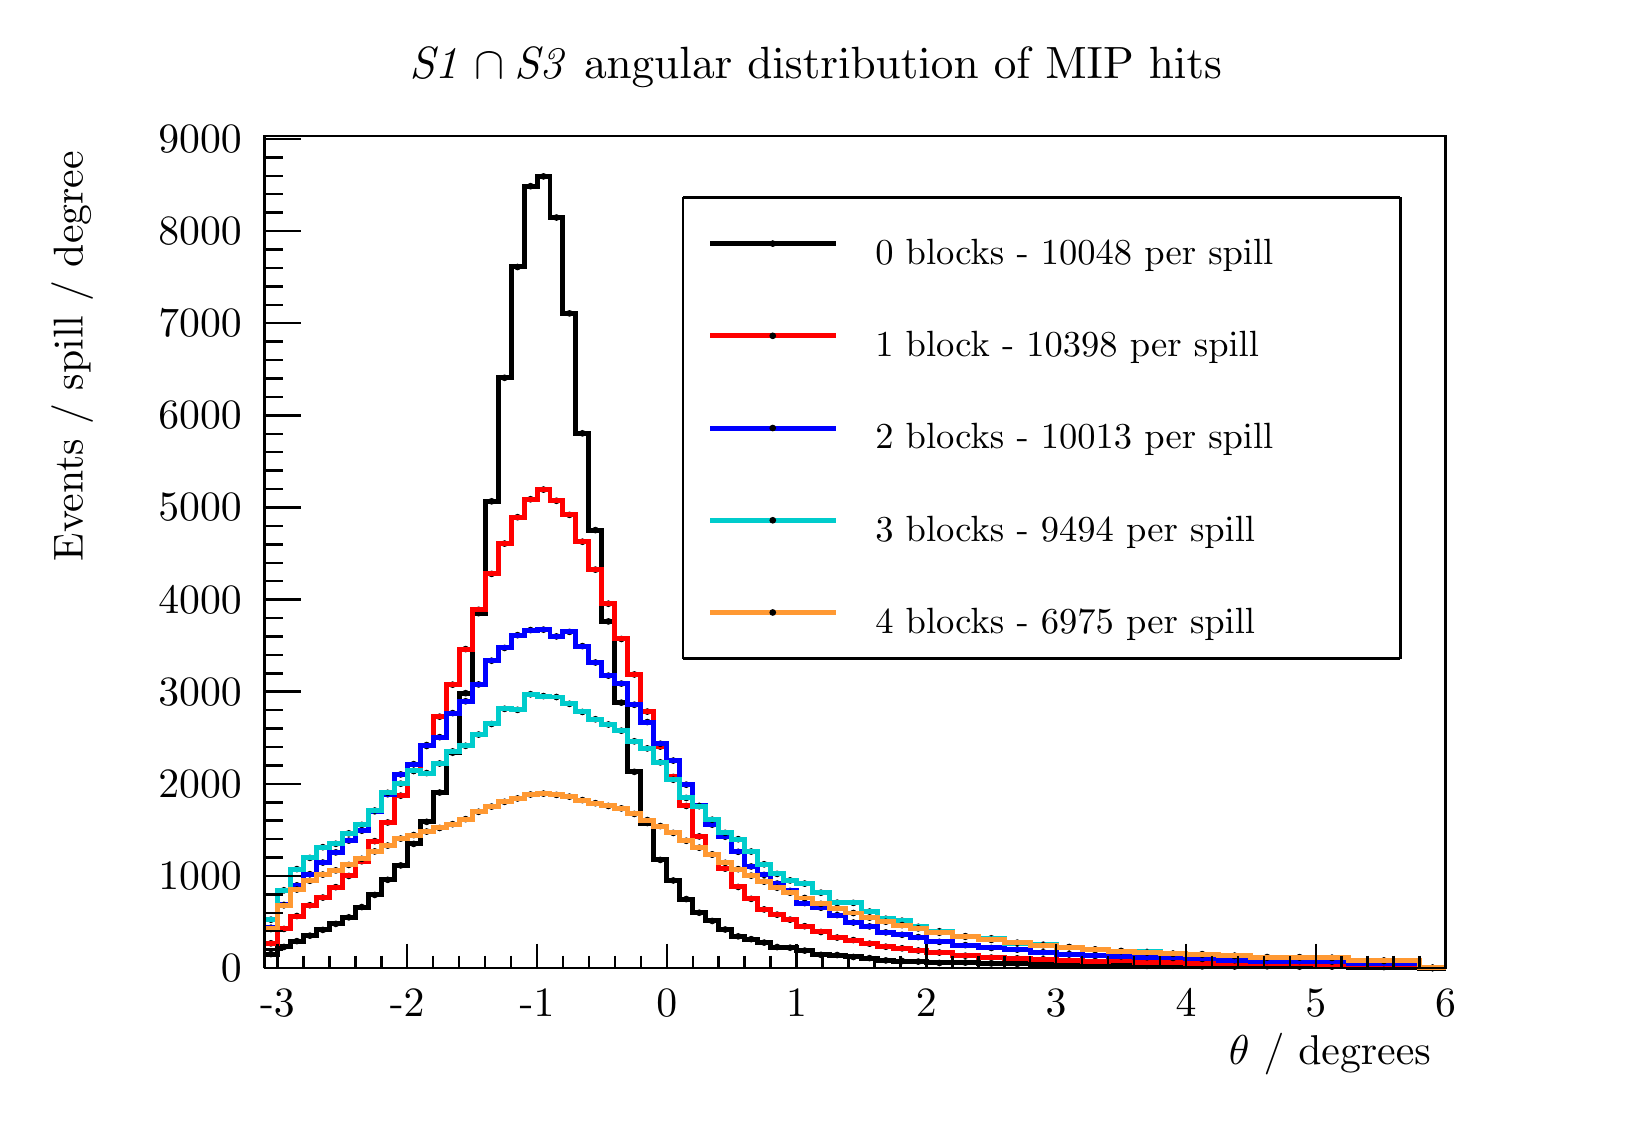
\begin{tikzpicture}
\pgfdeclareplotmark{cross} {
\pgfpathmoveto{\pgfpoint{-0.3\pgfplotmarksize}{\pgfplotmarksize}}
\pgfpathlineto{\pgfpoint{+0.3\pgfplotmarksize}{\pgfplotmarksize}}
\pgfpathlineto{\pgfpoint{+0.3\pgfplotmarksize}{0.3\pgfplotmarksize}}
\pgfpathlineto{\pgfpoint{+1\pgfplotmarksize}{0.3\pgfplotmarksize}}
\pgfpathlineto{\pgfpoint{+1\pgfplotmarksize}{-0.3\pgfplotmarksize}}
\pgfpathlineto{\pgfpoint{+0.3\pgfplotmarksize}{-0.3\pgfplotmarksize}}
\pgfpathlineto{\pgfpoint{+0.3\pgfplotmarksize}{-1.\pgfplotmarksize}}
\pgfpathlineto{\pgfpoint{-0.3\pgfplotmarksize}{-1.\pgfplotmarksize}}
\pgfpathlineto{\pgfpoint{-0.3\pgfplotmarksize}{-0.3\pgfplotmarksize}}
\pgfpathlineto{\pgfpoint{-1.\pgfplotmarksize}{-0.3\pgfplotmarksize}}
\pgfpathlineto{\pgfpoint{-1.\pgfplotmarksize}{0.3\pgfplotmarksize}}
\pgfpathlineto{\pgfpoint{-0.3\pgfplotmarksize}{0.3\pgfplotmarksize}}
\pgfpathclose
\pgfusepathqstroke
}
\pgfdeclareplotmark{cross*} {
\pgfpathmoveto{\pgfpoint{-0.3\pgfplotmarksize}{\pgfplotmarksize}}
\pgfpathlineto{\pgfpoint{+0.3\pgfplotmarksize}{\pgfplotmarksize}}
\pgfpathlineto{\pgfpoint{+0.3\pgfplotmarksize}{0.3\pgfplotmarksize}}
\pgfpathlineto{\pgfpoint{+1\pgfplotmarksize}{0.3\pgfplotmarksize}}
\pgfpathlineto{\pgfpoint{+1\pgfplotmarksize}{-0.3\pgfplotmarksize}}
\pgfpathlineto{\pgfpoint{+0.3\pgfplotmarksize}{-0.3\pgfplotmarksize}}
\pgfpathlineto{\pgfpoint{+0.3\pgfplotmarksize}{-1.\pgfplotmarksize}}
\pgfpathlineto{\pgfpoint{-0.3\pgfplotmarksize}{-1.\pgfplotmarksize}}
\pgfpathlineto{\pgfpoint{-0.3\pgfplotmarksize}{-0.3\pgfplotmarksize}}
\pgfpathlineto{\pgfpoint{-1.\pgfplotmarksize}{-0.3\pgfplotmarksize}}
\pgfpathlineto{\pgfpoint{-1.\pgfplotmarksize}{0.3\pgfplotmarksize}}
\pgfpathlineto{\pgfpoint{-0.3\pgfplotmarksize}{0.3\pgfplotmarksize}}
\pgfpathclose
\pgfusepathqfillstroke
}
\pgfdeclareplotmark{newstar} {
\pgfpathmoveto{\pgfqpoint{0pt}{\pgfplotmarksize}}
\pgfpathlineto{\pgfqpointpolar{44}{0.5\pgfplotmarksize}}
\pgfpathlineto{\pgfqpointpolar{18}{\pgfplotmarksize}}
\pgfpathlineto{\pgfqpointpolar{-20}{0.5\pgfplotmarksize}}
\pgfpathlineto{\pgfqpointpolar{-54}{\pgfplotmarksize}}
\pgfpathlineto{\pgfqpointpolar{-90}{0.5\pgfplotmarksize}}
\pgfpathlineto{\pgfqpointpolar{234}{\pgfplotmarksize}}
\pgfpathlineto{\pgfqpointpolar{198}{0.5\pgfplotmarksize}}
\pgfpathlineto{\pgfqpointpolar{162}{\pgfplotmarksize}}
\pgfpathlineto{\pgfqpointpolar{134}{0.5\pgfplotmarksize}}
\pgfpathclose
\pgfusepathqstroke
}
\pgfdeclareplotmark{newstar*} {
\pgfpathmoveto{\pgfqpoint{0pt}{\pgfplotmarksize}}
\pgfpathlineto{\pgfqpointpolar{44}{0.5\pgfplotmarksize}}
\pgfpathlineto{\pgfqpointpolar{18}{\pgfplotmarksize}}
\pgfpathlineto{\pgfqpointpolar{-20}{0.5\pgfplotmarksize}}
\pgfpathlineto{\pgfqpointpolar{-54}{\pgfplotmarksize}}
\pgfpathlineto{\pgfqpointpolar{-90}{0.5\pgfplotmarksize}}
\pgfpathlineto{\pgfqpointpolar{234}{\pgfplotmarksize}}
\pgfpathlineto{\pgfqpointpolar{198}{0.5\pgfplotmarksize}}
\pgfpathlineto{\pgfqpointpolar{162}{\pgfplotmarksize}}
\pgfpathlineto{\pgfqpointpolar{134}{0.5\pgfplotmarksize}}
\pgfpathclose
\pgfusepathqfillstroke
}
\definecolor{c}{rgb}{1,1,1};
\draw [color=c, fill=c] (0,0) rectangle (20,13.7199);
\draw [color=c, fill=c] (3,1.78359) rectangle (18,12.3479);
\definecolor{c}{rgb}{0,0,0};
\draw [c,line width=0.9] (3,1.78359) -- (3,12.3479) -- (18,12.3479) -- (18,1.78359) -- (3,1.78359);
\definecolor{c}{rgb}{1,1,1};
\draw [color=c, fill=c] (3,1.78359) rectangle (18,12.3479);
\definecolor{c}{rgb}{0,0,0};
\draw [c,line width=0.9] (3,1.78359) -- (3,12.3479) -- (18,12.3479) -- (18,1.78359) -- (3,1.78359);
\definecolor{c}{rgb}{0,0,0.6};
\draw [c,line width=0.9] (3,1.78359) -- (3.16484,1.78359) -- (3.16484,1.78359) -- (3.32967,1.78359) -- (3.32967,1.78359) -- (3.49451,1.78359) -- (3.49451,1.78359) -- (3.65934,1.78359) -- (3.65934,1.78359) -- (3.82418,1.78359) -- (3.82418,1.78359) --
 (3.98901,1.78359) -- (3.98901,1.78359) -- (4.15385,1.78359) -- (4.15385,1.78359) -- (4.31868,1.78359) -- (4.31868,1.78359) -- (4.48352,1.78359) -- (4.48352,1.78359) -- (4.64835,1.78359) -- (4.64835,1.78359) -- (4.81319,1.78359) -- (4.81319,1.78359)
 -- (4.97802,1.78359) -- (4.97802,1.78359) -- (5.14286,1.78359) -- (5.14286,1.78359) -- (5.30769,1.78359) -- (5.30769,1.78359) -- (5.47253,1.78359) -- (5.47253,1.78359) -- (5.63736,1.78359) -- (5.63736,1.78359) -- (5.8022,1.78359) -- (5.8022,1.78359)
 -- (5.96703,1.78359) -- (5.96703,1.78359) -- (6.13187,1.78359) -- (6.13187,1.78359) -- (6.2967,1.78359) -- (6.2967,1.78359) -- (6.46154,1.78359) -- (6.46154,1.78359) -- (6.62637,1.78359) -- (6.62637,1.78359) -- (6.79121,1.78359) -- (6.79121,1.78359)
 -- (6.95604,1.78359) -- (6.95604,1.78359) -- (7.12088,1.78359) -- (7.12088,1.78359) -- (7.28571,1.78359) -- (7.28571,1.78359) -- (7.45055,1.78359) -- (7.45055,1.78359) -- (7.61538,1.78359) -- (7.61538,1.78359) -- (7.78022,1.78359) --
 (7.78022,1.78359) -- (7.94506,1.78359) -- (7.94506,1.78359) -- (8.10989,1.78359) -- (8.10989,1.78359) -- (8.27472,1.78359) -- (8.27472,1.78359) -- (8.43956,1.78359) -- (8.43956,1.78359) -- (8.6044,1.78359) -- (8.6044,1.78359) -- (8.76923,1.78359) --
 (8.76923,1.78359) -- (8.93407,1.78359) -- (8.93407,1.78359) -- (9.0989,1.78359) -- (9.0989,1.78359) -- (9.26374,1.78359) -- (9.26374,1.78359) -- (9.42857,1.78359) -- (9.42857,1.78359) -- (9.59341,1.78359) -- (9.59341,1.78359) -- (9.75824,1.78359) --
 (9.75824,1.78359) -- (9.96429,1.78359) -- (9.96429,1.78359) -- (10.1703,1.78359) -- (10.1703,1.78359) -- (10.3764,1.78359) -- (10.3764,1.78359) -- (10.5824,1.78359) -- (10.5824,1.78359) -- (10.7885,1.78359) -- (10.7885,1.78359) -- (10.9945,1.78359)
 -- (10.9945,1.78359) -- (11.2005,1.78359) -- (11.2005,1.78359) -- (11.4066,1.78359) -- (11.4066,1.78359) -- (11.7363,1.78359) -- (11.7363,1.78359) -- (12.0659,1.78359) -- (12.0659,1.78359) -- (12.3956,1.78359) -- (12.3956,1.78359) --
 (12.7253,1.78359) -- (12.7253,1.78359) -- (13.0549,1.78359) -- (13.0549,1.78359) -- (13.3846,1.78359) -- (13.3846,1.78359) -- (13.7143,1.78359) -- (13.7143,1.78359) -- (14.044,1.78359) -- (14.044,1.78359) -- (14.3736,1.78359) -- (14.3736,1.78359) --
 (14.7033,1.78359) -- (14.7033,1.78359) -- (15.1154,1.78359) -- (15.1154,1.78359) -- (15.5275,1.78359) -- (15.5275,1.78359) -- (15.9396,1.78359) -- (15.9396,1.78359) -- (16.3516,1.78359) -- (16.3516,1.78359) -- (16.7637,1.78359) -- (16.7637,1.78359)
 -- (17.6703,1.78359) -- (17.6703,1.78359) -- (18,1.78359);
\definecolor{c}{rgb}{0,0,0};
\draw [c,line width=0.9] (3,1.78359) -- (18,1.78359);
\draw [c,line width=0.9] (3.16484,2.09229) -- (3.16484,1.78359);
\draw [c,line width=0.9] (3.49451,1.93794) -- (3.49451,1.78359);
\draw [c,line width=0.9] (3.82418,1.93794) -- (3.82418,1.78359);
\draw [c,line width=0.9] (4.15385,1.93794) -- (4.15385,1.78359);
\draw [c,line width=0.9] (4.48352,1.93794) -- (4.48352,1.78359);
\draw [c,line width=0.9] (4.81319,2.09229) -- (4.81319,1.78359);
\draw [c,line width=0.9] (5.14286,1.93794) -- (5.14286,1.78359);
\draw [c,line width=0.9] (5.47253,1.93794) -- (5.47253,1.78359);
\draw [c,line width=0.9] (5.8022,1.93794) -- (5.8022,1.78359);
\draw [c,line width=0.9] (6.13187,1.93794) -- (6.13187,1.78359);
\draw [c,line width=0.9] (6.46154,2.09229) -- (6.46154,1.78359);
\draw [c,line width=0.9] (6.79121,1.93794) -- (6.79121,1.78359);
\draw [c,line width=0.9] (7.12088,1.93794) -- (7.12088,1.78359);
\draw [c,line width=0.9] (7.45055,1.93794) -- (7.45055,1.78359);
\draw [c,line width=0.9] (7.78022,1.93794) -- (7.78022,1.78359);
\draw [c,line width=0.9] (8.10989,2.09229) -- (8.10989,1.78359);
\draw [c,line width=0.9] (8.43956,1.93794) -- (8.43956,1.78359);
\draw [c,line width=0.9] (8.76923,1.93794) -- (8.76923,1.78359);
\draw [c,line width=0.9] (9.0989,1.93794) -- (9.0989,1.78359);
\draw [c,line width=0.9] (9.42857,1.93794) -- (9.42857,1.78359);
\draw [c,line width=0.9] (9.75824,2.09229) -- (9.75824,1.78359);
\draw [c,line width=0.9] (10.0879,1.93794) -- (10.0879,1.78359);
\draw [c,line width=0.9] (10.4176,1.93794) -- (10.4176,1.78359);
\draw [c,line width=0.9] (10.7473,1.93794) -- (10.7473,1.78359);
\draw [c,line width=0.9] (11.0769,1.93794) -- (11.0769,1.78359);
\draw [c,line width=0.9] (11.4066,2.09229) -- (11.4066,1.78359);
\draw [c,line width=0.9] (11.7363,1.93794) -- (11.7363,1.78359);
\draw [c,line width=0.9] (12.0659,1.93794) -- (12.0659,1.78359);
\draw [c,line width=0.9] (12.3956,1.93794) -- (12.3956,1.78359);
\draw [c,line width=0.9] (12.7253,1.93794) -- (12.7253,1.78359);
\draw [c,line width=0.9] (13.0549,2.09229) -- (13.0549,1.78359);
\draw [c,line width=0.9] (13.3846,1.93794) -- (13.3846,1.78359);
\draw [c,line width=0.9] (13.7143,1.93794) -- (13.7143,1.78359);
\draw [c,line width=0.9] (14.044,1.93794) -- (14.044,1.78359);
\draw [c,line width=0.9] (14.3736,1.93794) -- (14.3736,1.78359);
\draw [c,line width=0.9] (14.7033,2.09229) -- (14.7033,1.78359);
\draw [c,line width=0.9] (15.033,1.93794) -- (15.033,1.78359);
\draw [c,line width=0.9] (15.3626,1.93794) -- (15.3626,1.78359);
\draw [c,line width=0.9] (15.6923,1.93794) -- (15.6923,1.78359);
\draw [c,line width=0.9] (16.022,1.93794) -- (16.022,1.78359);
\draw [c,line width=0.9] (16.3516,2.09229) -- (16.3516,1.78359);
\draw [c,line width=0.9] (16.6813,1.93794) -- (16.6813,1.78359);
\draw [c,line width=0.9] (17.011,1.93794) -- (17.011,1.78359);
\draw [c,line width=0.9] (17.3407,1.93794) -- (17.3407,1.78359);
\draw [c,line width=0.9] (17.6703,1.93794) -- (17.6703,1.78359);
\draw [c,line width=0.9] (18,2.09229) -- (18,1.78359);
\draw [c,line width=0.9] (3.16484,2.09229) -- (3.16484,1.78359);
\draw [anchor=base] (3.16484,1.1662) node[scale=1.50787, color=c, rotate=0]{-3};
\draw [anchor=base] (4.81319,1.1662) node[scale=1.50787, color=c, rotate=0]{-2};
\draw [anchor=base] (6.46154,1.1662) node[scale=1.50787, color=c, rotate=0]{-1};
\draw [anchor=base] (8.10989,1.1662) node[scale=1.50787, color=c, rotate=0]{0};
\draw [anchor=base] (9.75824,1.1662) node[scale=1.50787, color=c, rotate=0]{1};
\draw [anchor=base] (11.4066,1.1662) node[scale=1.50787, color=c, rotate=0]{2};
\draw [anchor=base] (13.0549,1.1662) node[scale=1.50787, color=c, rotate=0]{3};
\draw [anchor=base] (14.7033,1.1662) node[scale=1.50787, color=c, rotate=0]{4};
\draw [anchor=base] (16.3516,1.1662) node[scale=1.50787, color=c, rotate=0]{5};
\draw [anchor=base] (18,1.1662) node[scale=1.50787, color=c, rotate=0]{6};
\draw [anchor= east] (18,0.685997) node[scale=1.50787, color=c, rotate=0]{$\theta$ / degrees};
\draw [c,line width=0.9] (3,1.78359) -- (3,12.3479);
\draw [c,line width=0.9] (3.462,1.78359) -- (3,1.78359);
\draw [c,line width=0.9] (3.231,2.01758) -- (3,2.01758);
\draw [c,line width=0.9] (3.231,2.25157) -- (3,2.25157);
\draw [c,line width=0.9] (3.231,2.48557) -- (3,2.48557);
\draw [c,line width=0.9] (3.231,2.71956) -- (3,2.71956);
\draw [c,line width=0.9] (3.462,2.95355) -- (3,2.95355);
\draw [c,line width=0.9] (3.231,3.18754) -- (3,3.18754);
\draw [c,line width=0.9] (3.231,3.42153) -- (3,3.42153);
\draw [c,line width=0.9] (3.231,3.65552) -- (3,3.65552);
\draw [c,line width=0.9] (3.231,3.88951) -- (3,3.88951);
\draw [c,line width=0.9] (3.462,4.1235) -- (3,4.1235);
\draw [c,line width=0.9] (3.231,4.35749) -- (3,4.35749);
\draw [c,line width=0.9] (3.231,4.59148) -- (3,4.59148);
\draw [c,line width=0.9] (3.231,4.82548) -- (3,4.82548);
\draw [c,line width=0.9] (3.231,5.05947) -- (3,5.05947);
\draw [c,line width=0.9] (3.462,5.29346) -- (3,5.29346);
\draw [c,line width=0.9] (3.231,5.52745) -- (3,5.52745);
\draw [c,line width=0.9] (3.231,5.76144) -- (3,5.76144);
\draw [c,line width=0.9] (3.231,5.99543) -- (3,5.99543);
\draw [c,line width=0.9] (3.231,6.22942) -- (3,6.22942);
\draw [c,line width=0.9] (3.462,6.46341) -- (3,6.46341);
\draw [c,line width=0.9] (3.231,6.6974) -- (3,6.6974);
\draw [c,line width=0.9] (3.231,6.93139) -- (3,6.93139);
\draw [c,line width=0.9] (3.231,7.16539) -- (3,7.16539);
\draw [c,line width=0.9] (3.231,7.39938) -- (3,7.39938);
\draw [c,line width=0.9] (3.462,7.63337) -- (3,7.63337);
\draw [c,line width=0.9] (3.231,7.86736) -- (3,7.86736);
\draw [c,line width=0.9] (3.231,8.10135) -- (3,8.10135);
\draw [c,line width=0.9] (3.231,8.33534) -- (3,8.33534);
\draw [c,line width=0.9] (3.231,8.56933) -- (3,8.56933);
\draw [c,line width=0.9] (3.462,8.80332) -- (3,8.80332);
\draw [c,line width=0.9] (3.231,9.03731) -- (3,9.03731);
\draw [c,line width=0.9] (3.231,9.27131) -- (3,9.27131);
\draw [c,line width=0.9] (3.231,9.5053) -- (3,9.5053);
\draw [c,line width=0.9] (3.231,9.73929) -- (3,9.73929);
\draw [c,line width=0.9] (3.462,9.97328) -- (3,9.97328);
\draw [c,line width=0.9] (3.231,10.2073) -- (3,10.2073);
\draw [c,line width=0.9] (3.231,10.4413) -- (3,10.4413);
\draw [c,line width=0.9] (3.231,10.6753) -- (3,10.6753);
\draw [c,line width=0.9] (3.231,10.9092) -- (3,10.9092);
\draw [c,line width=0.9] (3.462,11.1432) -- (3,11.1432);
\draw [c,line width=0.9] (3.231,11.3772) -- (3,11.3772);
\draw [c,line width=0.9] (3.231,11.6112) -- (3,11.6112);
\draw [c,line width=0.9] (3.231,11.8452) -- (3,11.8452);
\draw [c,line width=0.9] (3.231,12.0792) -- (3,12.0792);
\draw [c,line width=0.9] (3.462,12.3132) -- (3,12.3132);
\draw [c,line width=0.9] (3.462,12.3132) -- (3,12.3132);
\draw [anchor= east] (2.9,1.78359) node[scale=1.50787, color=c, rotate=0]{0};
\draw [anchor= east] (2.9,2.95355) node[scale=1.50787, color=c, rotate=0]{1000};
\draw [anchor= east] (2.9,4.1235) node[scale=1.50787, color=c, rotate=0]{2000};
\draw [anchor= east] (2.9,5.29346) node[scale=1.50787, color=c, rotate=0]{3000};
\draw [anchor= east] (2.9,6.46341) node[scale=1.50787, color=c, rotate=0]{4000};
\draw [anchor= east] (2.9,7.63337) node[scale=1.50787, color=c, rotate=0]{5000};
\draw [anchor= east] (2.9,8.80332) node[scale=1.50787, color=c, rotate=0]{6000};
\draw [anchor= east] (2.9,9.97328) node[scale=1.50787, color=c, rotate=0]{7000};
\draw [anchor= east] (2.9,11.1432) node[scale=1.50787, color=c, rotate=0]{8000};
\draw [anchor= east] (2.9,12.3132) node[scale=1.50787, color=c, rotate=0]{9000};
\draw [anchor= east] (0.557284,12.3479) node[scale=1.50787, color=c, rotate=90]{ Events / spill / degree};
\draw [c,line width=1.8] (3.08242,1.96042) -- (3.08242,1.96133);
\draw [c,line width=1.8] (3.08242,1.96133) -- (3.08242,1.96225);
\foreach \P in {(3.08242,1.96133)}{\draw[mark options={color=c,fill=c},mark size=2.402402pt,mark=*,mark size=1pt] plot coordinates {\P};}
\draw [c,line width=1.8] (3.24725,2.05096) -- (3.24725,2.05209);
\draw [c,line width=1.8] (3.24725,2.05209) -- (3.24725,2.05321);
\foreach \P in {(3.24725,2.05209)}{\draw[mark options={color=c,fill=c},mark size=2.402402pt,mark=*,mark size=1pt] plot coordinates {\P};}
\draw [c,line width=1.8] (3.41209,2.1247) -- (3.41209,2.12597);
\draw [c,line width=1.8] (3.41209,2.12597) -- (3.41209,2.12724);
\foreach \P in {(3.41209,2.12597)}{\draw[mark options={color=c,fill=c},mark size=2.402402pt,mark=*,mark size=1pt] plot coordinates {\P};}
\draw [c,line width=1.8] (3.57692,2.19382) -- (3.57692,2.19522);
\draw [c,line width=1.8] (3.57692,2.19522) -- (3.57692,2.19662);
\foreach \P in {(3.57692,2.19522)}{\draw[mark options={color=c,fill=c},mark size=2.402402pt,mark=*,mark size=1pt] plot coordinates {\P};}
\draw [c,line width=1.8] (3.74176,2.26714) -- (3.74176,2.26865);
\draw [c,line width=1.8] (3.74176,2.26865) -- (3.74176,2.27017);
\foreach \P in {(3.74176,2.26865)}{\draw[mark options={color=c,fill=c},mark size=2.402402pt,mark=*,mark size=1pt] plot coordinates {\P};}
\draw [c,line width=1.8] (3.90659,2.34336) -- (3.90659,2.34499);
\draw [c,line width=1.8] (3.90659,2.34499) -- (3.90659,2.34662);
\foreach \P in {(3.90659,2.34499)}{\draw[mark options={color=c,fill=c},mark size=2.402402pt,mark=*,mark size=1pt] plot coordinates {\P};}
\draw [c,line width=1.8] (4.07143,2.42657) -- (4.07143,2.42831);
\draw [c,line width=1.8] (4.07143,2.42831) -- (4.07143,2.43004);
\foreach \P in {(4.07143,2.42831)}{\draw[mark options={color=c,fill=c},mark size=2.402402pt,mark=*,mark size=1pt] plot coordinates {\P};}
\draw [c,line width=1.8] (4.23626,2.55668) -- (4.23626,2.55859);
\draw [c,line width=1.8] (4.23626,2.55859) -- (4.23626,2.5605);
\foreach \P in {(4.23626,2.55859)}{\draw[mark options={color=c,fill=c},mark size=2.402402pt,mark=*,mark size=1pt] plot coordinates {\P};}
\draw [c,line width=1.8] (4.4011,2.71038) -- (4.4011,2.71247);
\draw [c,line width=1.8] (4.4011,2.71247) -- (4.4011,2.71456);
\foreach \P in {(4.4011,2.71247)}{\draw[mark options={color=c,fill=c},mark size=2.402402pt,mark=*,mark size=1pt] plot coordinates {\P};}
\draw [c,line width=1.8] (4.56593,2.90221) -- (4.56593,2.90451);
\draw [c,line width=1.8] (4.56593,2.90451) -- (4.56593,2.90682);
\foreach \P in {(4.56593,2.90451)}{\draw[mark options={color=c,fill=c},mark size=2.402402pt,mark=*,mark size=1pt] plot coordinates {\P};}
\draw [c,line width=1.8] (4.73077,3.08496) -- (4.73077,3.08744);
\draw [c,line width=1.8] (4.73077,3.08744) -- (4.73077,3.08992);
\foreach \P in {(4.73077,3.08744)}{\draw[mark options={color=c,fill=c},mark size=2.402402pt,mark=*,mark size=1pt] plot coordinates {\P};}
\draw [c,line width=1.8] (4.8956,3.35822) -- (4.8956,3.36094);
\draw [c,line width=1.8] (4.8956,3.36094) -- (4.8956,3.36367);
\foreach \P in {(4.8956,3.36094)}{\draw[mark options={color=c,fill=c},mark size=2.402402pt,mark=*,mark size=1pt] plot coordinates {\P};}
\draw [c,line width=1.8] (5.06044,3.63804) -- (5.06044,3.641);
\draw [c,line width=1.8] (5.06044,3.641) -- (5.06044,3.64396);
\foreach \P in {(5.06044,3.641)}{\draw[mark options={color=c,fill=c},mark size=2.402402pt,mark=*,mark size=1pt] plot coordinates {\P};}
\draw [c,line width=1.8] (5.22528,4.00993) -- (5.22528,4.01317);
\draw [c,line width=1.8] (5.22528,4.01317) -- (5.22528,4.01641);
\foreach \P in {(5.22528,4.01317)}{\draw[mark options={color=c,fill=c},mark size=2.402402pt,mark=*,mark size=1pt] plot coordinates {\P};}
\draw [c,line width=1.8] (5.39011,4.5153) -- (5.39011,4.5189);
\draw [c,line width=1.8] (5.39011,4.5189) -- (5.39011,4.52249);
\foreach \P in {(5.39011,4.5189)}{\draw[mark options={color=c,fill=c},mark size=2.402402pt,mark=*,mark size=1pt] plot coordinates {\P};}
\draw [c,line width=1.8] (5.55494,5.27113) -- (5.55494,5.27519);
\draw [c,line width=1.8] (5.55494,5.27519) -- (5.55494,5.27926);
\foreach \P in {(5.55494,5.27519)}{\draw[mark options={color=c,fill=c},mark size=2.402402pt,mark=*,mark size=1pt] plot coordinates {\P};}
\draw [c,line width=1.8] (5.71978,6.28683) -- (5.71978,6.29145);
\draw [c,line width=1.8] (5.71978,6.29145) -- (5.71978,6.29606);
\foreach \P in {(5.71978,6.29145)}{\draw[mark options={color=c,fill=c},mark size=2.402402pt,mark=*,mark size=1pt] plot coordinates {\P};}
\draw [c,line width=1.8] (5.88462,7.70618) -- (5.88462,7.71147);
\draw [c,line width=1.8] (5.88462,7.71147) -- (5.88462,7.71676);
\foreach \P in {(5.88462,7.71147)}{\draw[mark options={color=c,fill=c},mark size=2.402402pt,mark=*,mark size=1pt] plot coordinates {\P};}
\draw [c,line width=1.8] (6.04945,9.27429) -- (6.04945,9.28024);
\draw [c,line width=1.8] (6.04945,9.28024) -- (6.04945,9.28619);
\foreach \P in {(6.04945,9.28024)}{\draw[mark options={color=c,fill=c},mark size=2.402402pt,mark=*,mark size=1pt] plot coordinates {\P};}
\draw [c,line width=1.8] (6.21429,10.681) -- (6.21429,10.6875);
\draw [c,line width=1.8] (6.21429,10.6875) -- (6.21429,10.694);
\foreach \P in {(6.21429,10.6875)}{\draw[mark options={color=c,fill=c},mark size=2.402402pt,mark=*,mark size=1pt] plot coordinates {\P};}
\draw [c,line width=1.8] (6.37912,11.7069) -- (6.37912,11.7137);
\draw [c,line width=1.8] (6.37912,11.7137) -- (6.37912,11.7206);
\foreach \P in {(6.37912,11.7137)}{\draw[mark options={color=c,fill=c},mark size=2.402402pt,mark=*,mark size=1pt] plot coordinates {\P};}
\draw [c,line width=1.8] (6.54396,11.8311) -- (6.54396,11.838);
\draw [c,line width=1.8] (6.54396,11.838) -- (6.54396,11.8449);
\foreach \P in {(6.54396,11.838)}{\draw[mark options={color=c,fill=c},mark size=2.402402pt,mark=*,mark size=1pt] plot coordinates {\P};}
\draw [c,line width=1.8] (6.70879,11.3088) -- (6.70879,11.3155);
\draw [c,line width=1.8] (6.70879,11.3155) -- (6.70879,11.3222);
\foreach \P in {(6.70879,11.3155)}{\draw[mark options={color=c,fill=c},mark size=2.402402pt,mark=*,mark size=1pt] plot coordinates {\P};}
\draw [c,line width=1.8] (6.87363,10.0921) -- (6.87363,10.0984);
\draw [c,line width=1.8] (6.87363,10.0984) -- (6.87363,10.1047);
\foreach \P in {(6.87363,10.0984)}{\draw[mark options={color=c,fill=c},mark size=2.402402pt,mark=*,mark size=1pt] plot coordinates {\P};}
\draw [c,line width=1.8] (7.03846,8.56933) -- (7.03846,8.575);
\draw [c,line width=1.8] (7.03846,8.575) -- (7.03846,8.58066);
\foreach \P in {(7.03846,8.575)}{\draw[mark options={color=c,fill=c},mark size=2.402402pt,mark=*,mark size=1pt] plot coordinates {\P};}
\draw [c,line width=1.8] (7.2033,7.34089) -- (7.2033,7.34602);
\draw [c,line width=1.8] (7.2033,7.34602) -- (7.2033,7.35115);
\foreach \P in {(7.2033,7.34602)}{\draw[mark options={color=c,fill=c},mark size=2.402402pt,mark=*,mark size=1pt] plot coordinates {\P};}
\draw [c,line width=1.8] (7.36813,6.1819) -- (7.36813,6.18646);
\draw [c,line width=1.8] (7.36813,6.18646) -- (7.36813,6.19101);
\foreach \P in {(7.36813,6.18646)}{\draw[mark options={color=c,fill=c},mark size=2.402402pt,mark=*,mark size=1pt] plot coordinates {\P};}
\draw [c,line width=1.8] (7.53297,5.15058) -- (7.53297,5.15457);
\draw [c,line width=1.8] (7.53297,5.15457) -- (7.53297,5.15856);
\foreach \P in {(7.53297,5.15457)}{\draw[mark options={color=c,fill=c},mark size=2.402402pt,mark=*,mark size=1pt] plot coordinates {\P};}
\draw [c,line width=1.8] (7.6978,4.27259) -- (7.6978,4.27602);
\draw [c,line width=1.8] (7.6978,4.27602) -- (7.6978,4.27944);
\foreach \P in {(7.6978,4.27602)}{\draw[mark options={color=c,fill=c},mark size=2.402402pt,mark=*,mark size=1pt] plot coordinates {\P};}
\draw [c,line width=1.8] (7.86264,3.62309) -- (7.86264,3.62604);
\draw [c,line width=1.8] (7.86264,3.62604) -- (7.86264,3.62899);
\foreach \P in {(7.86264,3.62604)}{\draw[mark options={color=c,fill=c},mark size=2.402402pt,mark=*,mark size=1pt] plot coordinates {\P};}
\draw [c,line width=1.8] (8.02747,3.15496) -- (8.02747,3.15751);
\draw [c,line width=1.8] (8.02747,3.15751) -- (8.02747,3.16006);
\foreach \P in {(8.02747,3.15751)}{\draw[mark options={color=c,fill=c},mark size=2.402402pt,mark=*,mark size=1pt] plot coordinates {\P};}
\draw [c,line width=1.8] (8.19231,2.89398) -- (8.19231,2.89627);
\draw [c,line width=1.8] (8.19231,2.89627) -- (8.19231,2.89856);
\foreach \P in {(8.19231,2.89627)}{\draw[mark options={color=c,fill=c},mark size=2.402402pt,mark=*,mark size=1pt] plot coordinates {\P};}
\draw [c,line width=1.8] (8.35714,2.65818) -- (8.35714,2.66022);
\draw [c,line width=1.8] (8.35714,2.66022) -- (8.35714,2.66225);
\foreach \P in {(8.35714,2.66022)}{\draw[mark options={color=c,fill=c},mark size=2.402402pt,mark=*,mark size=1pt] plot coordinates {\P};}
\draw [c,line width=1.8] (8.52198,2.48491) -- (8.52198,2.48674);
\draw [c,line width=1.8] (8.52198,2.48674) -- (8.52198,2.48857);
\foreach \P in {(8.52198,2.48674)}{\draw[mark options={color=c,fill=c},mark size=2.402402pt,mark=*,mark size=1pt] plot coordinates {\P};}
\draw [c,line width=1.8] (8.68681,2.38063) -- (8.68681,2.38232);
\draw [c,line width=1.8] (8.68681,2.38232) -- (8.68681,2.384);
\foreach \P in {(8.68681,2.38232)}{\draw[mark options={color=c,fill=c},mark size=2.402402pt,mark=*,mark size=1pt] plot coordinates {\P};}
\draw [c,line width=1.8] (8.85165,2.272) -- (8.85165,2.27352);
\draw [c,line width=1.8] (8.85165,2.27352) -- (8.85165,2.27504);
\foreach \P in {(8.85165,2.27352)}{\draw[mark options={color=c,fill=c},mark size=2.402402pt,mark=*,mark size=1pt] plot coordinates {\P};}
\draw [c,line width=1.8] (9.01648,2.18553) -- (9.01648,2.18691);
\draw [c,line width=1.8] (9.01648,2.18691) -- (9.01648,2.1883);
\foreach \P in {(9.01648,2.18691)}{\draw[mark options={color=c,fill=c},mark size=2.402402pt,mark=*,mark size=1pt] plot coordinates {\P};}
\draw [c,line width=1.8] (9.18132,2.14992) -- (9.18132,2.15123);
\draw [c,line width=1.8] (9.18132,2.15123) -- (9.18132,2.15255);
\foreach \P in {(9.18132,2.15123)}{\draw[mark options={color=c,fill=c},mark size=2.402402pt,mark=*,mark size=1pt] plot coordinates {\P};}
\draw [c,line width=1.8] (9.34615,2.10613) -- (9.34615,2.10737);
\draw [c,line width=1.8] (9.34615,2.10737) -- (9.34615,2.10861);
\foreach \P in {(9.34615,2.10737)}{\draw[mark options={color=c,fill=c},mark size=2.402402pt,mark=*,mark size=1pt] plot coordinates {\P};}
\draw [c,line width=1.8] (9.51099,2.04971) -- (9.51099,2.05084);
\draw [c,line width=1.8] (9.51099,2.05084) -- (9.51099,2.05196);
\foreach \P in {(9.51099,2.05084)}{\draw[mark options={color=c,fill=c},mark size=2.402402pt,mark=*,mark size=1pt] plot coordinates {\P};}
\draw [c,line width=1.8] (9.67582,2.04139) -- (9.67582,2.0425);
\draw [c,line width=1.8] (9.67582,2.0425) -- (9.67582,2.04362);
\foreach \P in {(9.67582,2.0425)}{\draw[mark options={color=c,fill=c},mark size=2.402402pt,mark=*,mark size=1pt] plot coordinates {\P};}
\draw [c,line width=1.8] (9.86126,2.00446) -- (9.86126,2.0056);
\draw [c,line width=1.8] (9.86126,2.0056) -- (9.86126,2.00675);
\foreach \P in {(9.86126,2.0056)}{\draw[mark options={color=c,fill=c},mark size=2.402402pt,mark=*,mark size=1pt] plot coordinates {\P};}
\draw [c,line width=1.8] (10.0673,1.95095) -- (10.0673,1.95195);
\draw [c,line width=1.8] (10.0673,1.95195) -- (10.0673,1.95295);
\foreach \P in {(10.0673,1.95195)}{\draw[mark options={color=c,fill=c},mark size=2.402402pt,mark=*,mark size=1pt] plot coordinates {\P};}
\draw [c,line width=1.8] (10.2734,1.94837) -- (10.2734,1.94936);
\draw [c,line width=1.8] (10.2734,1.94936) -- (10.2734,1.95035);
\foreach \P in {(10.2734,1.94936)}{\draw[mark options={color=c,fill=c},mark size=2.402402pt,mark=*,mark size=1pt] plot coordinates {\P};}
\draw [c,line width=1.8] (10.4794,1.92407) -- (10.4794,1.92498);
\draw [c,line width=1.8] (10.4794,1.92498) -- (10.4794,1.92589);
\foreach \P in {(10.4794,1.92498)}{\draw[mark options={color=c,fill=c},mark size=2.402402pt,mark=*,mark size=1pt] plot coordinates {\P};}
\draw [c,line width=1.8] (10.6854,1.90959) -- (10.6854,1.91046);
\draw [c,line width=1.8] (10.6854,1.91046) -- (10.6854,1.91133);
\foreach \P in {(10.6854,1.91046)}{\draw[mark options={color=c,fill=c},mark size=2.402402pt,mark=*,mark size=1pt] plot coordinates {\P};}
\draw [c,line width=1.8] (10.8915,1.88035) -- (10.8915,1.88111);
\draw [c,line width=1.8] (10.8915,1.88111) -- (10.8915,1.88187);
\foreach \P in {(10.8915,1.88111)}{\draw[mark options={color=c,fill=c},mark size=2.402402pt,mark=*,mark size=1pt] plot coordinates {\P};}
\draw [c,line width=1.8] (11.0975,1.87278) -- (11.0975,1.87351);
\draw [c,line width=1.8] (11.0975,1.87351) -- (11.0975,1.87424);
\foreach \P in {(11.0975,1.87351)}{\draw[mark options={color=c,fill=c},mark size=2.402402pt,mark=*,mark size=1pt] plot coordinates {\P};}
\draw [c,line width=1.8] (11.3036,1.86516) -- (11.3036,1.86587);
\draw [c,line width=1.8] (11.3036,1.86587) -- (11.3036,1.86657);
\foreach \P in {(11.3036,1.86587)}{\draw[mark options={color=c,fill=c},mark size=2.402402pt,mark=*,mark size=1pt] plot coordinates {\P};}
\draw [c,line width=1.8] (11.5714,1.8481) -- (11.5714,1.84889);
\draw [c,line width=1.8] (11.5714,1.84889) -- (11.5714,1.84967);
\foreach \P in {(11.5714,1.84889)}{\draw[mark options={color=c,fill=c},mark size=2.402402pt,mark=*,mark size=1pt] plot coordinates {\P};}
\draw [c,line width=1.8] (11.9011,1.85223) -- (11.9011,1.85304);
\draw [c,line width=1.8] (11.9011,1.85304) -- (11.9011,1.85385);
\foreach \P in {(11.9011,1.85304)}{\draw[mark options={color=c,fill=c},mark size=2.402402pt,mark=*,mark size=1pt] plot coordinates {\P};}
\draw [c,line width=1.8] (12.2308,1.84206) -- (12.2308,1.84281);
\draw [c,line width=1.8] (12.2308,1.84281) -- (12.2308,1.84356);
\foreach \P in {(12.2308,1.84281)}{\draw[mark options={color=c,fill=c},mark size=2.402402pt,mark=*,mark size=1pt] plot coordinates {\P};}
\draw [c,line width=1.8] (12.5604,1.83622) -- (12.5604,1.83693);
\draw [c,line width=1.8] (12.5604,1.83693) -- (12.5604,1.83764);
\foreach \P in {(12.5604,1.83693)}{\draw[mark options={color=c,fill=c},mark size=2.402402pt,mark=*,mark size=1pt] plot coordinates {\P};}
\draw [c,line width=1.8] (12.8901,1.82585) -- (12.8901,1.82649);
\draw [c,line width=1.8] (12.8901,1.82649) -- (12.8901,1.82713);
\foreach \P in {(12.8901,1.82649)}{\draw[mark options={color=c,fill=c},mark size=2.402402pt,mark=*,mark size=1pt] plot coordinates {\P};}
\draw [c,line width=1.8] (13.2198,1.82341) -- (13.2198,1.82402);
\draw [c,line width=1.8] (13.2198,1.82402) -- (13.2198,1.82464);
\foreach \P in {(13.2198,1.82402)}{\draw[mark options={color=c,fill=c},mark size=2.402402pt,mark=*,mark size=1pt] plot coordinates {\P};}
\draw [c,line width=1.8] (13.5495,1.81898) -- (13.5495,1.81956);
\draw [c,line width=1.8] (13.5495,1.81956) -- (13.5495,1.82014);
\foreach \P in {(13.5495,1.81956)}{\draw[mark options={color=c,fill=c},mark size=2.402402pt,mark=*,mark size=1pt] plot coordinates {\P};}
\draw [c,line width=1.8] (13.8791,1.81696) -- (13.8791,1.81754);
\draw [c,line width=1.8] (13.8791,1.81754) -- (13.8791,1.81812);
\foreach \P in {(13.8791,1.81754)}{\draw[mark options={color=c,fill=c},mark size=2.402402pt,mark=*,mark size=1pt] plot coordinates {\P};}
\draw [c,line width=1.8] (14.2088,1.81084) -- (14.2088,1.81136);
\draw [c,line width=1.8] (14.2088,1.81136) -- (14.2088,1.81187);
\foreach \P in {(14.2088,1.81136)}{\draw[mark options={color=c,fill=c},mark size=2.402402pt,mark=*,mark size=1pt] plot coordinates {\P};}
\draw [c,line width=1.8] (14.5385,1.81226) -- (14.5385,1.81279);
\draw [c,line width=1.8] (14.5385,1.81279) -- (14.5385,1.81331);
\foreach \P in {(14.5385,1.81279)}{\draw[mark options={color=c,fill=c},mark size=2.402402pt,mark=*,mark size=1pt] plot coordinates {\P};}
\draw [c,line width=1.8] (14.9093,1.80551) -- (14.9093,1.80603);
\draw [c,line width=1.8] (14.9093,1.80603) -- (14.9093,1.80656);
\foreach \P in {(14.9093,1.80603)}{\draw[mark options={color=c,fill=c},mark size=2.402402pt,mark=*,mark size=1pt] plot coordinates {\P};}
\draw [c,line width=1.8] (15.3214,1.80324) -- (15.3214,1.80373);
\draw [c,line width=1.8] (15.3214,1.80373) -- (15.3214,1.80421);
\foreach \P in {(15.3214,1.80373)}{\draw[mark options={color=c,fill=c},mark size=2.402402pt,mark=*,mark size=1pt] plot coordinates {\P};}
\draw [c,line width=1.8] (15.7335,1.80624) -- (15.7335,1.80676);
\draw [c,line width=1.8] (15.7335,1.80676) -- (15.7335,1.80729);
\foreach \P in {(15.7335,1.80676)}{\draw[mark options={color=c,fill=c},mark size=2.402402pt,mark=*,mark size=1pt] plot coordinates {\P};}
\draw [c,line width=1.8] (16.1456,1.80134) -- (16.1456,1.8018);
\draw [c,line width=1.8] (16.1456,1.8018) -- (16.1456,1.80227);
\foreach \P in {(16.1456,1.8018)}{\draw[mark options={color=c,fill=c},mark size=2.402402pt,mark=*,mark size=1pt] plot coordinates {\P};}
\draw [c,line width=1.8] (16.5577,1.80172) -- (16.5577,1.80219);
\draw [c,line width=1.8] (16.5577,1.80219) -- (16.5577,1.80265);
\foreach \P in {(16.5577,1.80219)}{\draw[mark options={color=c,fill=c},mark size=2.402402pt,mark=*,mark size=1pt] plot coordinates {\P};}
\draw [c,line width=1.8] (17.217,1.79545) -- (17.217,1.79602);
\draw [c,line width=1.8] (17.217,1.79602) -- (17.217,1.79658);
\foreach \P in {(17.217,1.79602)}{\draw[mark options={color=c,fill=c},mark size=2.402402pt,mark=*,mark size=1pt] plot coordinates {\P};}
\draw [c,line width=1.8] (17.8352,1.78436) -- (17.8352,1.78458);
\draw [c,line width=1.8] (17.8352,1.78458) -- (17.8352,1.7848);
\foreach \P in {(17.8352,1.78458)}{\draw[mark options={color=c,fill=c},mark size=2.402402pt,mark=*,mark size=1pt] plot coordinates {\P};}
\draw [c,line width=1.8] (3,1.96133) -- (3.16484,1.96133) -- (3.16484,2.05209) -- (3.32967,2.05209) -- (3.32967,2.12597) -- (3.49451,2.12597) -- (3.49451,2.19522) -- (3.65934,2.19522) -- (3.65934,2.26865) -- (3.82418,2.26865) -- (3.82418,2.34499) --
 (3.98901,2.34499) -- (3.98901,2.42831) -- (4.15385,2.42831) -- (4.15385,2.55859) -- (4.31868,2.55859) -- (4.31868,2.71247) -- (4.48352,2.71247) -- (4.48352,2.90451) -- (4.64835,2.90451) -- (4.64835,3.08744) -- (4.81319,3.08744) -- (4.81319,3.36094)
 -- (4.97802,3.36094) -- (4.97802,3.641) -- (5.14286,3.641) -- (5.14286,4.01317) -- (5.30769,4.01317) -- (5.30769,4.5189) -- (5.47253,4.5189) -- (5.47253,5.27519) -- (5.63736,5.27519) -- (5.63736,6.29145) -- (5.8022,6.29145) -- (5.8022,7.71147) --
 (5.96703,7.71147) -- (5.96703,9.28024) -- (6.13187,9.28024) -- (6.13187,10.6875) -- (6.2967,10.6875) -- (6.2967,11.7137) -- (6.46154,11.7137) -- (6.46154,11.838) -- (6.62637,11.838) -- (6.62637,11.3155) -- (6.79121,11.3155) -- (6.79121,10.0984) --
 (6.95604,10.0984) -- (6.95604,8.575) -- (7.12088,8.575) -- (7.12088,7.34602) -- (7.28571,7.34602) -- (7.28571,6.18646) -- (7.45055,6.18646) -- (7.45055,5.15457) -- (7.61538,5.15457) -- (7.61538,4.27602) -- (7.78022,4.27602) -- (7.78022,3.62604) --
 (7.94506,3.62604) -- (7.94506,3.15751) -- (8.10989,3.15751) -- (8.10989,2.89627) -- (8.27472,2.89627) -- (8.27472,2.66022) -- (8.43956,2.66022) -- (8.43956,2.48674) -- (8.6044,2.48674) -- (8.6044,2.38232) -- (8.76923,2.38232) -- (8.76923,2.27352) --
 (8.93407,2.27352) -- (8.93407,2.18691) -- (9.0989,2.18691) -- (9.0989,2.15123) -- (9.26374,2.15123) -- (9.26374,2.10737) -- (9.42857,2.10737) -- (9.42857,2.05084) -- (9.59341,2.05084) -- (9.59341,2.0425) -- (9.75824,2.0425) -- (9.75824,2.0056) --
 (9.96429,2.0056) -- (9.96429,1.95195) -- (10.1703,1.95195) -- (10.1703,1.94936) -- (10.3764,1.94936) -- (10.3764,1.92498) -- (10.5824,1.92498) -- (10.5824,1.91046) -- (10.7885,1.91046) -- (10.7885,1.88111) -- (10.9945,1.88111) -- (10.9945,1.87351)
 -- (11.2005,1.87351) -- (11.2005,1.86587) -- (11.4066,1.86587) -- (11.4066,1.84889) -- (11.7363,1.84889) -- (11.7363,1.85304) -- (12.0659,1.85304) -- (12.0659,1.84281) -- (12.3956,1.84281) -- (12.3956,1.83693) -- (12.7253,1.83693) --
 (12.7253,1.82649) -- (13.0549,1.82649) -- (13.0549,1.82402) -- (13.3846,1.82402) -- (13.3846,1.81956) -- (13.7143,1.81956) -- (13.7143,1.81754) -- (14.044,1.81754) -- (14.044,1.81136) -- (14.3736,1.81136) -- (14.3736,1.81279) -- (14.7033,1.81279) --
 (14.7033,1.80603) -- (15.1154,1.80603) -- (15.1154,1.80373) -- (15.5275,1.80373) -- (15.5275,1.80676) -- (15.9396,1.80676) -- (15.9396,1.8018) -- (16.3516,1.8018) -- (16.3516,1.80219) -- (16.7637,1.80219) -- (16.7637,1.79602) -- (17.6703,1.79602) --
 (17.6703,1.78359) -- (18,1.78359);
\definecolor{c}{rgb}{1,0,0};
\draw [c,line width=1.8] (3.08242,2.09714) -- (3.08242,2.09815);
\draw [c,line width=1.8] (3.08242,2.09815) -- (3.08242,2.09916);
\definecolor{c}{rgb}{0,0,0};
\foreach \P in {(3.08242,2.09815)}{\draw[mark options={color=c,fill=c},mark size=2.402402pt,mark=*,mark size=1pt] plot coordinates {\P};}
\definecolor{c}{rgb}{1,0,0};
\draw [c,line width=1.8] (3.24725,2.27948) -- (3.24725,2.28075);
\draw [c,line width=1.8] (3.24725,2.28075) -- (3.24725,2.28201);
\definecolor{c}{rgb}{0,0,0};
\foreach \P in {(3.24725,2.28075)}{\draw[mark options={color=c,fill=c},mark size=2.402402pt,mark=*,mark size=1pt] plot coordinates {\P};}
\definecolor{c}{rgb}{1,0,0};
\draw [c,line width=1.8] (3.41209,2.4435) -- (3.41209,2.44497);
\draw [c,line width=1.8] (3.41209,2.44497) -- (3.41209,2.44643);
\definecolor{c}{rgb}{0,0,0};
\foreach \P in {(3.41209,2.44497)}{\draw[mark options={color=c,fill=c},mark size=2.402402pt,mark=*,mark size=1pt] plot coordinates {\P};}
\definecolor{c}{rgb}{1,0,0};
\draw [c,line width=1.8] (3.57692,2.58039) -- (3.57692,2.582);
\draw [c,line width=1.8] (3.57692,2.582) -- (3.57692,2.58361);
\definecolor{c}{rgb}{0,0,0};
\foreach \P in {(3.57692,2.582)}{\draw[mark options={color=c,fill=c},mark size=2.402402pt,mark=*,mark size=1pt] plot coordinates {\P};}
\definecolor{c}{rgb}{1,0,0};
\draw [c,line width=1.8] (3.74176,2.67742) -- (3.74176,2.67912);
\draw [c,line width=1.8] (3.74176,2.67912) -- (3.74176,2.68082);
\definecolor{c}{rgb}{0,0,0};
\foreach \P in {(3.74176,2.67912)}{\draw[mark options={color=c,fill=c},mark size=2.402402pt,mark=*,mark size=1pt] plot coordinates {\P};}
\definecolor{c}{rgb}{1,0,0};
\draw [c,line width=1.8] (3.90659,2.80977) -- (3.90659,2.8116);
\draw [c,line width=1.8] (3.90659,2.8116) -- (3.90659,2.81342);
\definecolor{c}{rgb}{0,0,0};
\foreach \P in {(3.90659,2.8116)}{\draw[mark options={color=c,fill=c},mark size=2.402402pt,mark=*,mark size=1pt] plot coordinates {\P};}
\definecolor{c}{rgb}{1,0,0};
\draw [c,line width=1.8] (4.07143,2.95225) -- (4.07143,2.9542);
\draw [c,line width=1.8] (4.07143,2.9542) -- (4.07143,2.95615);
\definecolor{c}{rgb}{0,0,0};
\foreach \P in {(4.07143,2.9542)}{\draw[mark options={color=c,fill=c},mark size=2.402402pt,mark=*,mark size=1pt] plot coordinates {\P};}
\definecolor{c}{rgb}{1,0,0};
\draw [c,line width=1.8] (4.23626,3.13862) -- (4.23626,3.14071);
\draw [c,line width=1.8] (4.23626,3.14071) -- (4.23626,3.14281);
\definecolor{c}{rgb}{0,0,0};
\foreach \P in {(4.23626,3.14071)}{\draw[mark options={color=c,fill=c},mark size=2.402402pt,mark=*,mark size=1pt] plot coordinates {\P};}
\definecolor{c}{rgb}{1,0,0};
\draw [c,line width=1.8] (4.4011,3.39362) -- (4.4011,3.39591);
\draw [c,line width=1.8] (4.4011,3.39591) -- (4.4011,3.3982);
\definecolor{c}{rgb}{0,0,0};
\foreach \P in {(4.4011,3.39591)}{\draw[mark options={color=c,fill=c},mark size=2.402402pt,mark=*,mark size=1pt] plot coordinates {\P};}
\definecolor{c}{rgb}{1,0,0};
\draw [c,line width=1.8] (4.56593,3.63056) -- (4.56593,3.63301);
\draw [c,line width=1.8] (4.56593,3.63301) -- (4.56593,3.63546);
\definecolor{c}{rgb}{0,0,0};
\foreach \P in {(4.56593,3.63301)}{\draw[mark options={color=c,fill=c},mark size=2.402402pt,mark=*,mark size=1pt] plot coordinates {\P};}
\definecolor{c}{rgb}{1,0,0};
\draw [c,line width=1.8] (4.73077,3.97085) -- (4.73077,3.97351);
\draw [c,line width=1.8] (4.73077,3.97351) -- (4.73077,3.97617);
\definecolor{c}{rgb}{0,0,0};
\foreach \P in {(4.73077,3.97351)}{\draw[mark options={color=c,fill=c},mark size=2.402402pt,mark=*,mark size=1pt] plot coordinates {\P};}
\definecolor{c}{rgb}{1,0,0};
\draw [c,line width=1.8] (4.8956,4.28388) -- (4.8956,4.28673);
\draw [c,line width=1.8] (4.8956,4.28673) -- (4.8956,4.28957);
\definecolor{c}{rgb}{0,0,0};
\foreach \P in {(4.8956,4.28673)}{\draw[mark options={color=c,fill=c},mark size=2.402402pt,mark=*,mark size=1pt] plot coordinates {\P};}
\definecolor{c}{rgb}{1,0,0};
\draw [c,line width=1.8] (5.06044,4.6015) -- (5.06044,4.60452);
\draw [c,line width=1.8] (5.06044,4.60452) -- (5.06044,4.60754);
\definecolor{c}{rgb}{0,0,0};
\foreach \P in {(5.06044,4.60452)}{\draw[mark options={color=c,fill=c},mark size=2.402402pt,mark=*,mark size=1pt] plot coordinates {\P};}
\definecolor{c}{rgb}{1,0,0};
\draw [c,line width=1.8] (5.22528,4.97306) -- (5.22528,4.97628);
\draw [c,line width=1.8] (5.22528,4.97628) -- (5.22528,4.97949);
\definecolor{c}{rgb}{0,0,0};
\foreach \P in {(5.22528,4.97628)}{\draw[mark options={color=c,fill=c},mark size=2.402402pt,mark=*,mark size=1pt] plot coordinates {\P};}
\definecolor{c}{rgb}{1,0,0};
\draw [c,line width=1.8] (5.39011,5.37934) -- (5.39011,5.38275);
\draw [c,line width=1.8] (5.39011,5.38275) -- (5.39011,5.38617);
\definecolor{c}{rgb}{0,0,0};
\foreach \P in {(5.39011,5.38275)}{\draw[mark options={color=c,fill=c},mark size=2.402402pt,mark=*,mark size=1pt] plot coordinates {\P};}
\definecolor{c}{rgb}{1,0,0};
\draw [c,line width=1.8] (5.55494,5.83124) -- (5.55494,5.83486);
\draw [c,line width=1.8] (5.55494,5.83486) -- (5.55494,5.83847);
\definecolor{c}{rgb}{0,0,0};
\foreach \P in {(5.55494,5.83486)}{\draw[mark options={color=c,fill=c},mark size=2.402402pt,mark=*,mark size=1pt] plot coordinates {\P};}
\definecolor{c}{rgb}{1,0,0};
\draw [c,line width=1.8] (5.71978,6.32959) -- (5.71978,6.33342);
\draw [c,line width=1.8] (5.71978,6.33342) -- (5.71978,6.33725);
\definecolor{c}{rgb}{0,0,0};
\foreach \P in {(5.71978,6.33342)}{\draw[mark options={color=c,fill=c},mark size=2.402402pt,mark=*,mark size=1pt] plot coordinates {\P};}
\definecolor{c}{rgb}{1,0,0};
\draw [c,line width=1.8] (5.88462,6.78597) -- (5.88462,6.78999);
\draw [c,line width=1.8] (5.88462,6.78999) -- (5.88462,6.79401);
\definecolor{c}{rgb}{0,0,0};
\foreach \P in {(5.88462,6.78999)}{\draw[mark options={color=c,fill=c},mark size=2.402402pt,mark=*,mark size=1pt] plot coordinates {\P};}
\definecolor{c}{rgb}{1,0,0};
\draw [c,line width=1.8] (6.04945,7.1706) -- (6.04945,7.17477);
\draw [c,line width=1.8] (6.04945,7.17477) -- (6.04945,7.17894);
\definecolor{c}{rgb}{0,0,0};
\foreach \P in {(6.04945,7.17477)}{\draw[mark options={color=c,fill=c},mark size=2.402402pt,mark=*,mark size=1pt] plot coordinates {\P};}
\definecolor{c}{rgb}{1,0,0};
\draw [c,line width=1.8] (6.21429,7.50559) -- (6.21429,7.50989);
\draw [c,line width=1.8] (6.21429,7.50989) -- (6.21429,7.51419);
\definecolor{c}{rgb}{0,0,0};
\foreach \P in {(6.21429,7.50989)}{\draw[mark options={color=c,fill=c},mark size=2.402402pt,mark=*,mark size=1pt] plot coordinates {\P};}
\definecolor{c}{rgb}{1,0,0};
\draw [c,line width=1.8] (6.37912,7.73355) -- (6.37912,7.73794);
\draw [c,line width=1.8] (6.37912,7.73794) -- (6.37912,7.74233);
\definecolor{c}{rgb}{0,0,0};
\foreach \P in {(6.37912,7.73794)}{\draw[mark options={color=c,fill=c},mark size=2.402402pt,mark=*,mark size=1pt] plot coordinates {\P};}
\definecolor{c}{rgb}{1,0,0};
\draw [c,line width=1.8] (6.54396,7.856) -- (6.54396,7.86043);
\draw [c,line width=1.8] (6.54396,7.86043) -- (6.54396,7.86486);
\definecolor{c}{rgb}{0,0,0};
\foreach \P in {(6.54396,7.86043)}{\draw[mark options={color=c,fill=c},mark size=2.402402pt,mark=*,mark size=1pt] plot coordinates {\P};}
\definecolor{c}{rgb}{1,0,0};
\draw [c,line width=1.8] (6.70879,7.71375) -- (6.70879,7.71814);
\draw [c,line width=1.8] (6.70879,7.71814) -- (6.70879,7.72252);
\definecolor{c}{rgb}{0,0,0};
\foreach \P in {(6.70879,7.71814)}{\draw[mark options={color=c,fill=c},mark size=2.402402pt,mark=*,mark size=1pt] plot coordinates {\P};}
\definecolor{c}{rgb}{1,0,0};
\draw [c,line width=1.8] (6.87363,7.53514) -- (6.87363,7.53945);
\draw [c,line width=1.8] (6.87363,7.53945) -- (6.87363,7.54376);
\definecolor{c}{rgb}{0,0,0};
\foreach \P in {(6.87363,7.53945)}{\draw[mark options={color=c,fill=c},mark size=2.402402pt,mark=*,mark size=1pt] plot coordinates {\P};}
\definecolor{c}{rgb}{1,0,0};
\draw [c,line width=1.8] (7.03846,7.1942) -- (7.03846,7.19838);
\draw [c,line width=1.8] (7.03846,7.19838) -- (7.03846,7.20256);
\definecolor{c}{rgb}{0,0,0};
\foreach \P in {(7.03846,7.19838)}{\draw[mark options={color=c,fill=c},mark size=2.402402pt,mark=*,mark size=1pt] plot coordinates {\P};}
\definecolor{c}{rgb}{1,0,0};
\draw [c,line width=1.8] (7.2033,6.8398) -- (7.2033,6.84384);
\draw [c,line width=1.8] (7.2033,6.84384) -- (7.2033,6.84788);
\definecolor{c}{rgb}{0,0,0};
\foreach \P in {(7.2033,6.84384)}{\draw[mark options={color=c,fill=c},mark size=2.402402pt,mark=*,mark size=1pt] plot coordinates {\P};}
\definecolor{c}{rgb}{1,0,0};
\draw [c,line width=1.8] (7.36813,6.40726) -- (7.36813,6.41113);
\draw [c,line width=1.8] (7.36813,6.41113) -- (7.36813,6.41499);
\definecolor{c}{rgb}{0,0,0};
\foreach \P in {(7.36813,6.41113)}{\draw[mark options={color=c,fill=c},mark size=2.402402pt,mark=*,mark size=1pt] plot coordinates {\P};}
\definecolor{c}{rgb}{1,0,0};
\draw [c,line width=1.8] (7.53297,5.95964) -- (7.53297,5.96331);
\draw [c,line width=1.8] (7.53297,5.96331) -- (7.53297,5.96699);
\definecolor{c}{rgb}{0,0,0};
\foreach \P in {(7.53297,5.96331)}{\draw[mark options={color=c,fill=c},mark size=2.402402pt,mark=*,mark size=1pt] plot coordinates {\P};}
\definecolor{c}{rgb}{1,0,0};
\draw [c,line width=1.8] (7.6978,5.50906) -- (7.6978,5.51253);
\draw [c,line width=1.8] (7.6978,5.51253) -- (7.6978,5.51599);
\definecolor{c}{rgb}{0,0,0};
\foreach \P in {(7.6978,5.51253)}{\draw[mark options={color=c,fill=c},mark size=2.402402pt,mark=*,mark size=1pt] plot coordinates {\P};}
\definecolor{c}{rgb}{1,0,0};
\draw [c,line width=1.8] (7.86264,5.03779) -- (7.86264,5.04103);
\draw [c,line width=1.8] (7.86264,5.04103) -- (7.86264,5.04427);
\definecolor{c}{rgb}{0,0,0};
\foreach \P in {(7.86264,5.04103)}{\draw[mark options={color=c,fill=c},mark size=2.402402pt,mark=*,mark size=1pt] plot coordinates {\P};}
\definecolor{c}{rgb}{1,0,0};
\draw [c,line width=1.8] (8.02747,4.59326) -- (8.02747,4.59628);
\draw [c,line width=1.8] (8.02747,4.59628) -- (8.02747,4.59929);
\definecolor{c}{rgb}{0,0,0};
\foreach \P in {(8.02747,4.59628)}{\draw[mark options={color=c,fill=c},mark size=2.402402pt,mark=*,mark size=1pt] plot coordinates {\P};}
\definecolor{c}{rgb}{1,0,0};
\draw [c,line width=1.8] (8.19231,4.20832) -- (8.19231,4.21113);
\draw [c,line width=1.8] (8.19231,4.21113) -- (8.19231,4.21393);
\definecolor{c}{rgb}{0,0,0};
\foreach \P in {(8.19231,4.21113)}{\draw[mark options={color=c,fill=c},mark size=2.402402pt,mark=*,mark size=1pt] plot coordinates {\P};}
\definecolor{c}{rgb}{1,0,0};
\draw [c,line width=1.8] (8.35714,3.84025) -- (8.35714,3.84283);
\draw [c,line width=1.8] (8.35714,3.84283) -- (8.35714,3.8454);
\definecolor{c}{rgb}{0,0,0};
\foreach \P in {(8.35714,3.84283)}{\draw[mark options={color=c,fill=c},mark size=2.402402pt,mark=*,mark size=1pt] plot coordinates {\P};}
\definecolor{c}{rgb}{1,0,0};
\draw [c,line width=1.8] (8.52198,3.45334) -- (8.52198,3.45567);
\draw [c,line width=1.8] (8.52198,3.45567) -- (8.52198,3.45799);
\definecolor{c}{rgb}{0,0,0};
\foreach \P in {(8.52198,3.45567)}{\draw[mark options={color=c,fill=c},mark size=2.402402pt,mark=*,mark size=1pt] plot coordinates {\P};}
\definecolor{c}{rgb}{1,0,0};
\draw [c,line width=1.8] (8.68681,3.2251) -- (8.68681,3.22726);
\draw [c,line width=1.8] (8.68681,3.22726) -- (8.68681,3.22942);
\definecolor{c}{rgb}{0,0,0};
\foreach \P in {(8.68681,3.22726)}{\draw[mark options={color=c,fill=c},mark size=2.402402pt,mark=*,mark size=1pt] plot coordinates {\P};}
\definecolor{c}{rgb}{1,0,0};
\draw [c,line width=1.8] (8.85165,3.04516) -- (8.85165,3.04718);
\draw [c,line width=1.8] (8.85165,3.04718) -- (8.85165,3.0492);
\definecolor{c}{rgb}{0,0,0};
\foreach \P in {(8.85165,3.04718)}{\draw[mark options={color=c,fill=c},mark size=2.402402pt,mark=*,mark size=1pt] plot coordinates {\P};}
\definecolor{c}{rgb}{1,0,0};
\draw [c,line width=1.8] (9.01648,2.81245) -- (9.01648,2.81428);
\draw [c,line width=1.8] (9.01648,2.81428) -- (9.01648,2.81611);
\definecolor{c}{rgb}{0,0,0};
\foreach \P in {(9.01648,2.81428)}{\draw[mark options={color=c,fill=c},mark size=2.402402pt,mark=*,mark size=1pt] plot coordinates {\P};}
\definecolor{c}{rgb}{1,0,0};
\draw [c,line width=1.8] (9.18132,2.66138) -- (9.18132,2.66306);
\draw [c,line width=1.8] (9.18132,2.66306) -- (9.18132,2.66475);
\definecolor{c}{rgb}{0,0,0};
\foreach \P in {(9.18132,2.66306)}{\draw[mark options={color=c,fill=c},mark size=2.402402pt,mark=*,mark size=1pt] plot coordinates {\P};}
\definecolor{c}{rgb}{1,0,0};
\draw [c,line width=1.8] (9.34615,2.52706) -- (9.34615,2.52861);
\draw [c,line width=1.8] (9.34615,2.52861) -- (9.34615,2.53016);
\definecolor{c}{rgb}{0,0,0};
\foreach \P in {(9.34615,2.52861)}{\draw[mark options={color=c,fill=c},mark size=2.402402pt,mark=*,mark size=1pt] plot coordinates {\P};}
\definecolor{c}{rgb}{1,0,0};
\draw [c,line width=1.8] (9.51099,2.46034) -- (9.51099,2.46183);
\draw [c,line width=1.8] (9.51099,2.46183) -- (9.51099,2.46331);
\definecolor{c}{rgb}{0,0,0};
\foreach \P in {(9.51099,2.46183)}{\draw[mark options={color=c,fill=c},mark size=2.402402pt,mark=*,mark size=1pt] plot coordinates {\P};}
\definecolor{c}{rgb}{1,0,0};
\draw [c,line width=1.8] (9.67582,2.3973) -- (9.67582,2.39871);
\draw [c,line width=1.8] (9.67582,2.39871) -- (9.67582,2.40012);
\definecolor{c}{rgb}{0,0,0};
\foreach \P in {(9.67582,2.39871)}{\draw[mark options={color=c,fill=c},mark size=2.402402pt,mark=*,mark size=1pt] plot coordinates {\P};}
\definecolor{c}{rgb}{1,0,0};
\draw [c,line width=1.8] (9.86126,2.31431) -- (9.86126,2.31578);
\draw [c,line width=1.8] (9.86126,2.31578) -- (9.86126,2.31724);
\definecolor{c}{rgb}{0,0,0};
\foreach \P in {(9.86126,2.31578)}{\draw[mark options={color=c,fill=c},mark size=2.402402pt,mark=*,mark size=1pt] plot coordinates {\P};}
\definecolor{c}{rgb}{1,0,0};
\draw [c,line width=1.8] (10.0673,2.24077) -- (10.0673,2.24213);
\draw [c,line width=1.8] (10.0673,2.24213) -- (10.0673,2.24349);
\definecolor{c}{rgb}{0,0,0};
\foreach \P in {(10.0673,2.24213)}{\draw[mark options={color=c,fill=c},mark size=2.402402pt,mark=*,mark size=1pt] plot coordinates {\P};}
\definecolor{c}{rgb}{1,0,0};
\draw [c,line width=1.8] (10.2734,2.16998) -- (10.2734,2.17124);
\draw [c,line width=1.8] (10.2734,2.17124) -- (10.2734,2.17249);
\definecolor{c}{rgb}{0,0,0};
\foreach \P in {(10.2734,2.17124)}{\draw[mark options={color=c,fill=c},mark size=2.402402pt,mark=*,mark size=1pt] plot coordinates {\P};}
\definecolor{c}{rgb}{1,0,0};
\draw [c,line width=1.8] (10.4794,2.13818) -- (10.4794,2.13938);
\draw [c,line width=1.8] (10.4794,2.13938) -- (10.4794,2.14058);
\definecolor{c}{rgb}{0,0,0};
\foreach \P in {(10.4794,2.13938)}{\draw[mark options={color=c,fill=c},mark size=2.402402pt,mark=*,mark size=1pt] plot coordinates {\P};}
\definecolor{c}{rgb}{1,0,0};
\draw [c,line width=1.8] (10.6854,2.09282) -- (10.6854,2.09394);
\draw [c,line width=1.8] (10.6854,2.09394) -- (10.6854,2.09507);
\definecolor{c}{rgb}{0,0,0};
\foreach \P in {(10.6854,2.09394)}{\draw[mark options={color=c,fill=c},mark size=2.402402pt,mark=*,mark size=1pt] plot coordinates {\P};}
\definecolor{c}{rgb}{1,0,0};
\draw [c,line width=1.8] (10.8915,2.05389) -- (10.8915,2.05493);
\draw [c,line width=1.8] (10.8915,2.05493) -- (10.8915,2.05597);
\definecolor{c}{rgb}{0,0,0};
\foreach \P in {(10.8915,2.05493)}{\draw[mark options={color=c,fill=c},mark size=2.402402pt,mark=*,mark size=1pt] plot coordinates {\P};}
\definecolor{c}{rgb}{1,0,0};
\draw [c,line width=1.8] (11.0975,2.03371) -- (11.0975,2.03472);
\draw [c,line width=1.8] (11.0975,2.03472) -- (11.0975,2.03572);
\definecolor{c}{rgb}{0,0,0};
\foreach \P in {(11.0975,2.03472)}{\draw[mark options={color=c,fill=c},mark size=2.402402pt,mark=*,mark size=1pt] plot coordinates {\P};}
\definecolor{c}{rgb}{1,0,0};
\draw [c,line width=1.8] (11.3036,2.00608) -- (11.3036,2.00703);
\draw [c,line width=1.8] (11.3036,2.00703) -- (11.3036,2.00797);
\definecolor{c}{rgb}{0,0,0};
\foreach \P in {(11.3036,2.00703)}{\draw[mark options={color=c,fill=c},mark size=2.402402pt,mark=*,mark size=1pt] plot coordinates {\P};}
\definecolor{c}{rgb}{1,0,0};
\draw [c,line width=1.8] (11.5714,1.97989) -- (11.5714,1.98102);
\draw [c,line width=1.8] (11.5714,1.98102) -- (11.5714,1.98214);
\definecolor{c}{rgb}{0,0,0};
\foreach \P in {(11.5714,1.98102)}{\draw[mark options={color=c,fill=c},mark size=2.402402pt,mark=*,mark size=1pt] plot coordinates {\P};}
\definecolor{c}{rgb}{1,0,0};
\draw [c,line width=1.8] (11.9011,1.93989) -- (11.9011,1.9409);
\draw [c,line width=1.8] (11.9011,1.9409) -- (11.9011,1.94191);
\definecolor{c}{rgb}{0,0,0};
\foreach \P in {(11.9011,1.9409)}{\draw[mark options={color=c,fill=c},mark size=2.402402pt,mark=*,mark size=1pt] plot coordinates {\P};}
\definecolor{c}{rgb}{1,0,0};
\draw [c,line width=1.8] (12.2308,1.91581) -- (12.2308,1.91674);
\draw [c,line width=1.8] (12.2308,1.91674) -- (12.2308,1.91767);
\definecolor{c}{rgb}{0,0,0};
\foreach \P in {(12.2308,1.91674)}{\draw[mark options={color=c,fill=c},mark size=2.402402pt,mark=*,mark size=1pt] plot coordinates {\P};}
\definecolor{c}{rgb}{1,0,0};
\draw [c,line width=1.8] (12.5604,1.90642) -- (12.5604,1.90732);
\draw [c,line width=1.8] (12.5604,1.90732) -- (12.5604,1.90821);
\definecolor{c}{rgb}{0,0,0};
\foreach \P in {(12.5604,1.90732)}{\draw[mark options={color=c,fill=c},mark size=2.402402pt,mark=*,mark size=1pt] plot coordinates {\P};}
\definecolor{c}{rgb}{1,0,0};
\draw [c,line width=1.8] (12.8901,1.89523) -- (12.8901,1.89609);
\draw [c,line width=1.8] (12.8901,1.89609) -- (12.8901,1.89694);
\definecolor{c}{rgb}{0,0,0};
\foreach \P in {(12.8901,1.89609)}{\draw[mark options={color=c,fill=c},mark size=2.402402pt,mark=*,mark size=1pt] plot coordinates {\P};}
\definecolor{c}{rgb}{1,0,0};
\draw [c,line width=1.8] (13.2198,1.87942) -- (13.2198,1.88021);
\draw [c,line width=1.8] (13.2198,1.88021) -- (13.2198,1.881);
\definecolor{c}{rgb}{0,0,0};
\foreach \P in {(13.2198,1.88021)}{\draw[mark options={color=c,fill=c},mark size=2.402402pt,mark=*,mark size=1pt] plot coordinates {\P};}
\definecolor{c}{rgb}{1,0,0};
\draw [c,line width=1.8] (13.5495,1.87219) -- (13.5495,1.87295);
\draw [c,line width=1.8] (13.5495,1.87295) -- (13.5495,1.87371);
\definecolor{c}{rgb}{0,0,0};
\foreach \P in {(13.5495,1.87295)}{\draw[mark options={color=c,fill=c},mark size=2.402402pt,mark=*,mark size=1pt] plot coordinates {\P};}
\definecolor{c}{rgb}{1,0,0};
\draw [c,line width=1.8] (13.8791,1.87478) -- (13.8791,1.87555);
\draw [c,line width=1.8] (13.8791,1.87555) -- (13.8791,1.87632);
\definecolor{c}{rgb}{0,0,0};
\foreach \P in {(13.8791,1.87555)}{\draw[mark options={color=c,fill=c},mark size=2.402402pt,mark=*,mark size=1pt] plot coordinates {\P};}
\definecolor{c}{rgb}{1,0,0};
\draw [c,line width=1.8] (14.2088,1.85406) -- (14.2088,1.85474);
\draw [c,line width=1.8] (14.2088,1.85474) -- (14.2088,1.85542);
\definecolor{c}{rgb}{0,0,0};
\foreach \P in {(14.2088,1.85474)}{\draw[mark options={color=c,fill=c},mark size=2.402402pt,mark=*,mark size=1pt] plot coordinates {\P};}
\definecolor{c}{rgb}{1,0,0};
\draw [c,line width=1.8] (14.5385,1.85869) -- (14.5385,1.85938);
\draw [c,line width=1.8] (14.5385,1.85938) -- (14.5385,1.86008);
\definecolor{c}{rgb}{0,0,0};
\foreach \P in {(14.5385,1.85938)}{\draw[mark options={color=c,fill=c},mark size=2.402402pt,mark=*,mark size=1pt] plot coordinates {\P};}
\definecolor{c}{rgb}{1,0,0};
\draw [c,line width=1.8] (14.9093,1.8404) -- (14.9093,1.84108);
\draw [c,line width=1.8] (14.9093,1.84108) -- (14.9093,1.84177);
\definecolor{c}{rgb}{0,0,0};
\foreach \P in {(14.9093,1.84108)}{\draw[mark options={color=c,fill=c},mark size=2.402402pt,mark=*,mark size=1pt] plot coordinates {\P};}
\definecolor{c}{rgb}{1,0,0};
\draw [c,line width=1.8] (15.3214,1.84042) -- (15.3214,1.84111);
\draw [c,line width=1.8] (15.3214,1.84111) -- (15.3214,1.84179);
\definecolor{c}{rgb}{0,0,0};
\foreach \P in {(15.3214,1.84111)}{\draw[mark options={color=c,fill=c},mark size=2.402402pt,mark=*,mark size=1pt] plot coordinates {\P};}
\definecolor{c}{rgb}{1,0,0};
\draw [c,line width=1.8] (15.7335,1.83506) -- (15.7335,1.83571);
\draw [c,line width=1.8] (15.7335,1.83571) -- (15.7335,1.83636);
\definecolor{c}{rgb}{0,0,0};
\foreach \P in {(15.7335,1.83571)}{\draw[mark options={color=c,fill=c},mark size=2.402402pt,mark=*,mark size=1pt] plot coordinates {\P};}
\definecolor{c}{rgb}{1,0,0};
\draw [c,line width=1.8] (16.1456,1.83527) -- (16.1456,1.83591);
\draw [c,line width=1.8] (16.1456,1.83591) -- (16.1456,1.83656);
\definecolor{c}{rgb}{0,0,0};
\foreach \P in {(16.1456,1.83591)}{\draw[mark options={color=c,fill=c},mark size=2.402402pt,mark=*,mark size=1pt] plot coordinates {\P};}
\definecolor{c}{rgb}{1,0,0};
\draw [c,line width=1.8] (16.5577,1.83409) -- (16.5577,1.83473);
\draw [c,line width=1.8] (16.5577,1.83473) -- (16.5577,1.83538);
\definecolor{c}{rgb}{0,0,0};
\foreach \P in {(16.5577,1.83473)}{\draw[mark options={color=c,fill=c},mark size=2.402402pt,mark=*,mark size=1pt] plot coordinates {\P};}
\definecolor{c}{rgb}{1,0,0};
\draw [c,line width=1.8] (17.217,1.81844) -- (17.217,1.81924);
\draw [c,line width=1.8] (17.217,1.81924) -- (17.217,1.82004);
\definecolor{c}{rgb}{0,0,0};
\foreach \P in {(17.217,1.81924)}{\draw[mark options={color=c,fill=c},mark size=2.402402pt,mark=*,mark size=1pt] plot coordinates {\P};}
\definecolor{c}{rgb}{1,0,0};
\draw [c,line width=1.8] (17.8352,1.7846) -- (17.8352,1.7848);
\draw [c,line width=1.8] (17.8352,1.7848) -- (17.8352,1.785);
\definecolor{c}{rgb}{0,0,0};
\foreach \P in {(17.8352,1.7848)}{\draw[mark options={color=c,fill=c},mark size=2.402402pt,mark=*,mark size=1pt] plot coordinates {\P};}
\definecolor{c}{rgb}{1,0,0};
\draw [c,line width=1.8] (3,2.09815) -- (3.16484,2.09815) -- (3.16484,2.28075) -- (3.32967,2.28075) -- (3.32967,2.44497) -- (3.49451,2.44497) -- (3.49451,2.582) -- (3.65934,2.582) -- (3.65934,2.67912) -- (3.82418,2.67912) -- (3.82418,2.8116) --
 (3.98901,2.8116) -- (3.98901,2.9542) -- (4.15385,2.9542) -- (4.15385,3.14071) -- (4.31868,3.14071) -- (4.31868,3.39591) -- (4.48352,3.39591) -- (4.48352,3.63301) -- (4.64835,3.63301) -- (4.64835,3.97351) -- (4.81319,3.97351) -- (4.81319,4.28673) --
 (4.97802,4.28673) -- (4.97802,4.60452) -- (5.14286,4.60452) -- (5.14286,4.97628) -- (5.30769,4.97628) -- (5.30769,5.38275) -- (5.47253,5.38275) -- (5.47253,5.83486) -- (5.63736,5.83486) -- (5.63736,6.33342) -- (5.8022,6.33342) -- (5.8022,6.78999) --
 (5.96703,6.78999) -- (5.96703,7.17477) -- (6.13187,7.17477) -- (6.13187,7.50989) -- (6.2967,7.50989) -- (6.2967,7.73794) -- (6.46154,7.73794) -- (6.46154,7.86043) -- (6.62637,7.86043) -- (6.62637,7.71814) -- (6.79121,7.71814) -- (6.79121,7.53945) --
 (6.95604,7.53945) -- (6.95604,7.19838) -- (7.12088,7.19838) -- (7.12088,6.84384) -- (7.28571,6.84384) -- (7.28571,6.41113) -- (7.45055,6.41113) -- (7.45055,5.96331) -- (7.61538,5.96331) -- (7.61538,5.51253) -- (7.78022,5.51253) -- (7.78022,5.04103)
 -- (7.94506,5.04103) -- (7.94506,4.59628) -- (8.10989,4.59628) -- (8.10989,4.21113) -- (8.27472,4.21113) -- (8.27472,3.84283) -- (8.43956,3.84283) -- (8.43956,3.45567) -- (8.6044,3.45567) -- (8.6044,3.22726) -- (8.76923,3.22726) -- (8.76923,3.04718)
 -- (8.93407,3.04718) -- (8.93407,2.81428) -- (9.0989,2.81428) -- (9.0989,2.66306) -- (9.26374,2.66306) -- (9.26374,2.52861) -- (9.42857,2.52861) -- (9.42857,2.46183) -- (9.59341,2.46183) -- (9.59341,2.39871) -- (9.75824,2.39871) -- (9.75824,2.31578)
 -- (9.96429,2.31578) -- (9.96429,2.24213) -- (10.1703,2.24213) -- (10.1703,2.17124) -- (10.3764,2.17124) -- (10.3764,2.13938) -- (10.5824,2.13938) -- (10.5824,2.09394) -- (10.7885,2.09394) -- (10.7885,2.05493) -- (10.9945,2.05493) --
 (10.9945,2.03472) -- (11.2005,2.03472) -- (11.2005,2.00703) -- (11.4066,2.00703) -- (11.4066,1.98102) -- (11.7363,1.98102) -- (11.7363,1.9409) -- (12.0659,1.9409) -- (12.0659,1.91674) -- (12.3956,1.91674) -- (12.3956,1.90732) -- (12.7253,1.90732) --
 (12.7253,1.89609) -- (13.0549,1.89609) -- (13.0549,1.88021) -- (13.3846,1.88021) -- (13.3846,1.87295) -- (13.7143,1.87295) -- (13.7143,1.87555) -- (14.044,1.87555) -- (14.044,1.85474) -- (14.3736,1.85474) -- (14.3736,1.85938) -- (14.7033,1.85938) --
 (14.7033,1.84108) -- (15.1154,1.84108) -- (15.1154,1.84111) -- (15.5275,1.84111) -- (15.5275,1.83571) -- (15.9396,1.83571) -- (15.9396,1.83591) -- (16.3516,1.83591) -- (16.3516,1.83473) -- (16.7637,1.83473) -- (16.7637,1.81924) -- (17.6703,1.81924)
 -- (17.6703,1.7848) -- (18,1.7848);
\definecolor{c}{rgb}{0,0,1};
\draw [c,line width=1.8] (3.08242,2.29489) -- (3.08242,2.29611);
\draw [c,line width=1.8] (3.08242,2.29611) -- (3.08242,2.29732);
\definecolor{c}{rgb}{0,0,0};
\foreach \P in {(3.08242,2.29611)}{\draw[mark options={color=c,fill=c},mark size=2.402402pt,mark=*,mark size=1pt] plot coordinates {\P};}
\definecolor{c}{rgb}{0,0,1};
\draw [c,line width=1.8] (3.24725,2.58469) -- (3.24725,2.58621);
\draw [c,line width=1.8] (3.24725,2.58621) -- (3.24725,2.58772);
\definecolor{c}{rgb}{0,0,0};
\foreach \P in {(3.24725,2.58621)}{\draw[mark options={color=c,fill=c},mark size=2.402402pt,mark=*,mark size=1pt] plot coordinates {\P};}
\definecolor{c}{rgb}{0,0,1};
\draw [c,line width=1.8] (3.41209,2.83237) -- (3.41209,2.8341);
\draw [c,line width=1.8] (3.41209,2.8341) -- (3.41209,2.83583);
\definecolor{c}{rgb}{0,0,0};
\foreach \P in {(3.41209,2.8341)}{\draw[mark options={color=c,fill=c},mark size=2.402402pt,mark=*,mark size=1pt] plot coordinates {\P};}
\definecolor{c}{rgb}{0,0,1};
\draw [c,line width=1.8] (3.57692,2.97451) -- (3.57692,2.97635);
\draw [c,line width=1.8] (3.57692,2.97635) -- (3.57692,2.9782);
\definecolor{c}{rgb}{0,0,0};
\foreach \P in {(3.57692,2.97635)}{\draw[mark options={color=c,fill=c},mark size=2.402402pt,mark=*,mark size=1pt] plot coordinates {\P};}
\definecolor{c}{rgb}{0,0,1};
\draw [c,line width=1.8] (3.74176,3.12189) -- (3.74176,3.12384);
\draw [c,line width=1.8] (3.74176,3.12384) -- (3.74176,3.1258);
\definecolor{c}{rgb}{0,0,0};
\foreach \P in {(3.74176,3.12384)}{\draw[mark options={color=c,fill=c},mark size=2.402402pt,mark=*,mark size=1pt] plot coordinates {\P};}
\definecolor{c}{rgb}{0,0,1};
\draw [c,line width=1.8] (3.90659,3.25087) -- (3.90659,3.25293);
\draw [c,line width=1.8] (3.90659,3.25293) -- (3.90659,3.25498);
\definecolor{c}{rgb}{0,0,0};
\foreach \P in {(3.90659,3.25293)}{\draw[mark options={color=c,fill=c},mark size=2.402402pt,mark=*,mark size=1pt] plot coordinates {\P};}
\definecolor{c}{rgb}{0,0,1};
\draw [c,line width=1.8] (4.07143,3.40045) -- (4.07143,3.40261);
\draw [c,line width=1.8] (4.07143,3.40261) -- (4.07143,3.40476);
\definecolor{c}{rgb}{0,0,0};
\foreach \P in {(4.07143,3.40261)}{\draw[mark options={color=c,fill=c},mark size=2.402402pt,mark=*,mark size=1pt] plot coordinates {\P};}
\definecolor{c}{rgb}{0,0,1};
\draw [c,line width=1.8] (4.23626,3.52611) -- (4.23626,3.52835);
\draw [c,line width=1.8] (4.23626,3.52835) -- (4.23626,3.53058);
\definecolor{c}{rgb}{0,0,0};
\foreach \P in {(4.23626,3.52835)}{\draw[mark options={color=c,fill=c},mark size=2.402402pt,mark=*,mark size=1pt] plot coordinates {\P};}
\definecolor{c}{rgb}{0,0,1};
\draw [c,line width=1.8] (4.4011,3.77246) -- (4.4011,3.77485);
\draw [c,line width=1.8] (4.4011,3.77485) -- (4.4011,3.77723);
\definecolor{c}{rgb}{0,0,0};
\foreach \P in {(4.4011,3.77485)}{\draw[mark options={color=c,fill=c},mark size=2.402402pt,mark=*,mark size=1pt] plot coordinates {\P};}
\definecolor{c}{rgb}{0,0,1};
\draw [c,line width=1.8] (4.56593,3.98951) -- (4.56593,3.99202);
\draw [c,line width=1.8] (4.56593,3.99202) -- (4.56593,3.99454);
\definecolor{c}{rgb}{0,0,0};
\foreach \P in {(4.56593,3.99202)}{\draw[mark options={color=c,fill=c},mark size=2.402402pt,mark=*,mark size=1pt] plot coordinates {\P};}
\definecolor{c}{rgb}{0,0,1};
\draw [c,line width=1.8] (4.73077,4.24052) -- (4.73077,4.24317);
\draw [c,line width=1.8] (4.73077,4.24317) -- (4.73077,4.24583);
\definecolor{c}{rgb}{0,0,0};
\foreach \P in {(4.73077,4.24317)}{\draw[mark options={color=c,fill=c},mark size=2.402402pt,mark=*,mark size=1pt] plot coordinates {\P};}
\definecolor{c}{rgb}{0,0,1};
\draw [c,line width=1.8] (4.8956,4.37073) -- (4.8956,4.37346);
\draw [c,line width=1.8] (4.8956,4.37346) -- (4.8956,4.37618);
\definecolor{c}{rgb}{0,0,0};
\foreach \P in {(4.8956,4.37346)}{\draw[mark options={color=c,fill=c},mark size=2.402402pt,mark=*,mark size=1pt] plot coordinates {\P};}
\definecolor{c}{rgb}{0,0,1};
\draw [c,line width=1.8] (5.06044,4.61334) -- (5.06044,4.61619);
\draw [c,line width=1.8] (5.06044,4.61619) -- (5.06044,4.61904);
\definecolor{c}{rgb}{0,0,0};
\foreach \P in {(5.06044,4.61619)}{\draw[mark options={color=c,fill=c},mark size=2.402402pt,mark=*,mark size=1pt] plot coordinates {\P};}
\definecolor{c}{rgb}{0,0,1};
\draw [c,line width=1.8] (5.22528,4.71357) -- (5.22528,4.71646);
\draw [c,line width=1.8] (5.22528,4.71646) -- (5.22528,4.71936);
\definecolor{c}{rgb}{0,0,0};
\foreach \P in {(5.22528,4.71646)}{\draw[mark options={color=c,fill=c},mark size=2.402402pt,mark=*,mark size=1pt] plot coordinates {\P};}
\definecolor{c}{rgb}{0,0,1};
\draw [c,line width=1.8] (5.39011,5.01895) -- (5.39011,5.02201);
\draw [c,line width=1.8] (5.39011,5.02201) -- (5.39011,5.02506);
\definecolor{c}{rgb}{0,0,0};
\foreach \P in {(5.39011,5.02201)}{\draw[mark options={color=c,fill=c},mark size=2.402402pt,mark=*,mark size=1pt] plot coordinates {\P};}
\definecolor{c}{rgb}{0,0,1};
\draw [c,line width=1.8] (5.55494,5.16913) -- (5.55494,5.17224);
\draw [c,line width=1.8] (5.55494,5.17224) -- (5.55494,5.17536);
\definecolor{c}{rgb}{0,0,0};
\foreach \P in {(5.55494,5.17224)}{\draw[mark options={color=c,fill=c},mark size=2.402402pt,mark=*,mark size=1pt] plot coordinates {\P};}
\definecolor{c}{rgb}{0,0,1};
\draw [c,line width=1.8] (5.71978,5.38301) -- (5.71978,5.38623);
\draw [c,line width=1.8] (5.71978,5.38623) -- (5.71978,5.38945);
\definecolor{c}{rgb}{0,0,0};
\foreach \P in {(5.71978,5.38623)}{\draw[mark options={color=c,fill=c},mark size=2.402402pt,mark=*,mark size=1pt] plot coordinates {\P};}
\definecolor{c}{rgb}{0,0,1};
\draw [c,line width=1.8] (5.88462,5.68389) -- (5.88462,5.68724);
\draw [c,line width=1.8] (5.88462,5.68724) -- (5.88462,5.69058);
\definecolor{c}{rgb}{0,0,0};
\foreach \P in {(5.88462,5.68724)}{\draw[mark options={color=c,fill=c},mark size=2.402402pt,mark=*,mark size=1pt] plot coordinates {\P};}
\definecolor{c}{rgb}{0,0,1};
\draw [c,line width=1.8] (6.04945,5.84624) -- (6.04945,5.84965);
\draw [c,line width=1.8] (6.04945,5.84965) -- (6.04945,5.85307);
\definecolor{c}{rgb}{0,0,0};
\foreach \P in {(6.04945,5.84965)}{\draw[mark options={color=c,fill=c},mark size=2.402402pt,mark=*,mark size=1pt] plot coordinates {\P};}
\definecolor{c}{rgb}{0,0,1};
\draw [c,line width=1.8] (6.21429,6.00828) -- (6.21429,6.01177);
\draw [c,line width=1.8] (6.21429,6.01177) -- (6.21429,6.01525);
\definecolor{c}{rgb}{0,0,0};
\foreach \P in {(6.21429,6.01177)}{\draw[mark options={color=c,fill=c},mark size=2.402402pt,mark=*,mark size=1pt] plot coordinates {\P};}
\definecolor{c}{rgb}{0,0,1};
\draw [c,line width=1.8] (6.37912,6.07269) -- (6.37912,6.0762);
\draw [c,line width=1.8] (6.37912,6.0762) -- (6.37912,6.0797);
\definecolor{c}{rgb}{0,0,0};
\foreach \P in {(6.37912,6.0762)}{\draw[mark options={color=c,fill=c},mark size=2.402402pt,mark=*,mark size=1pt] plot coordinates {\P};}
\definecolor{c}{rgb}{0,0,1};
\draw [c,line width=1.8] (6.54396,6.07818) -- (6.54396,6.08169);
\draw [c,line width=1.8] (6.54396,6.08169) -- (6.54396,6.08519);
\definecolor{c}{rgb}{0,0,0};
\foreach \P in {(6.54396,6.08169)}{\draw[mark options={color=c,fill=c},mark size=2.402402pt,mark=*,mark size=1pt] plot coordinates {\P};}
\definecolor{c}{rgb}{0,0,1};
\draw [c,line width=1.8] (6.70879,5.99246) -- (6.70879,5.99594);
\draw [c,line width=1.8] (6.70879,5.99594) -- (6.70879,5.99941);
\definecolor{c}{rgb}{0,0,0};
\foreach \P in {(6.70879,5.99594)}{\draw[mark options={color=c,fill=c},mark size=2.402402pt,mark=*,mark size=1pt] plot coordinates {\P};}
\definecolor{c}{rgb}{0,0,1};
\draw [c,line width=1.8] (6.87363,6.0499) -- (6.87363,6.0534);
\draw [c,line width=1.8] (6.87363,6.0534) -- (6.87363,6.0569);
\definecolor{c}{rgb}{0,0,0};
\foreach \P in {(6.87363,6.0534)}{\draw[mark options={color=c,fill=c},mark size=2.402402pt,mark=*,mark size=1pt] plot coordinates {\P};}
\definecolor{c}{rgb}{0,0,1};
\draw [c,line width=1.8] (7.03846,5.86922) -- (7.03846,5.87264);
\draw [c,line width=1.8] (7.03846,5.87264) -- (7.03846,5.87607);
\definecolor{c}{rgb}{0,0,0};
\foreach \P in {(7.03846,5.87264)}{\draw[mark options={color=c,fill=c},mark size=2.402402pt,mark=*,mark size=1pt] plot coordinates {\P};}
\definecolor{c}{rgb}{0,0,1};
\draw [c,line width=1.8] (7.2033,5.6611) -- (7.2033,5.66443);
\draw [c,line width=1.8] (7.2033,5.66443) -- (7.2033,5.66777);
\definecolor{c}{rgb}{0,0,0};
\foreach \P in {(7.2033,5.66443)}{\draw[mark options={color=c,fill=c},mark size=2.402402pt,mark=*,mark size=1pt] plot coordinates {\P};}
\definecolor{c}{rgb}{0,0,1};
\draw [c,line width=1.8] (7.36813,5.49431) -- (7.36813,5.49757);
\draw [c,line width=1.8] (7.36813,5.49757) -- (7.36813,5.50083);
\definecolor{c}{rgb}{0,0,0};
\foreach \P in {(7.36813,5.49757)}{\draw[mark options={color=c,fill=c},mark size=2.402402pt,mark=*,mark size=1pt] plot coordinates {\P};}
\definecolor{c}{rgb}{0,0,1};
\draw [c,line width=1.8] (7.53297,5.39354) -- (7.53297,5.39675);
\draw [c,line width=1.8] (7.53297,5.39675) -- (7.53297,5.39997);
\definecolor{c}{rgb}{0,0,0};
\foreach \P in {(7.53297,5.39675)}{\draw[mark options={color=c,fill=c},mark size=2.402402pt,mark=*,mark size=1pt] plot coordinates {\P};}
\definecolor{c}{rgb}{0,0,1};
\draw [c,line width=1.8] (7.6978,5.1249) -- (7.6978,5.128);
\draw [c,line width=1.8] (7.6978,5.128) -- (7.6978,5.1311);
\definecolor{c}{rgb}{0,0,0};
\foreach \P in {(7.6978,5.128)}{\draw[mark options={color=c,fill=c},mark size=2.402402pt,mark=*,mark size=1pt] plot coordinates {\P};}
\definecolor{c}{rgb}{0,0,1};
\draw [c,line width=1.8] (7.86264,4.90527) -- (7.86264,4.90826);
\draw [c,line width=1.8] (7.86264,4.90826) -- (7.86264,4.91125);
\definecolor{c}{rgb}{0,0,0};
\foreach \P in {(7.86264,4.90826)}{\draw[mark options={color=c,fill=c},mark size=2.402402pt,mark=*,mark size=1pt] plot coordinates {\P};}
\definecolor{c}{rgb}{0,0,1};
\draw [c,line width=1.8] (8.02747,4.63) -- (8.02747,4.63285);
\draw [c,line width=1.8] (8.02747,4.63285) -- (8.02747,4.6357);
\definecolor{c}{rgb}{0,0,0};
\foreach \P in {(8.02747,4.63285)}{\draw[mark options={color=c,fill=c},mark size=2.402402pt,mark=*,mark size=1pt] plot coordinates {\P};}
\definecolor{c}{rgb}{0,0,1};
\draw [c,line width=1.8] (8.19231,4.41621) -- (8.19231,4.41896);
\draw [c,line width=1.8] (8.19231,4.41896) -- (8.19231,4.42171);
\definecolor{c}{rgb}{0,0,0};
\foreach \P in {(8.19231,4.41896)}{\draw[mark options={color=c,fill=c},mark size=2.402402pt,mark=*,mark size=1pt] plot coordinates {\P};}
\definecolor{c}{rgb}{0,0,1};
\draw [c,line width=1.8] (8.35714,4.11026) -- (8.35714,4.11284);
\draw [c,line width=1.8] (8.35714,4.11284) -- (8.35714,4.11543);
\definecolor{c}{rgb}{0,0,0};
\foreach \P in {(8.35714,4.11284)}{\draw[mark options={color=c,fill=c},mark size=2.402402pt,mark=*,mark size=1pt] plot coordinates {\P};}
\definecolor{c}{rgb}{0,0,1};
\draw [c,line width=1.8] (8.52198,3.84047) -- (8.52198,3.8429);
\draw [c,line width=1.8] (8.52198,3.8429) -- (8.52198,3.84533);
\definecolor{c}{rgb}{0,0,0};
\foreach \P in {(8.52198,3.8429)}{\draw[mark options={color=c,fill=c},mark size=2.402402pt,mark=*,mark size=1pt] plot coordinates {\P};}
\definecolor{c}{rgb}{0,0,1};
\draw [c,line width=1.8] (8.68681,3.60293) -- (8.68681,3.60521);
\draw [c,line width=1.8] (8.68681,3.60521) -- (8.68681,3.6075);
\definecolor{c}{rgb}{0,0,0};
\foreach \P in {(8.68681,3.60521)}{\draw[mark options={color=c,fill=c},mark size=2.402402pt,mark=*,mark size=1pt] plot coordinates {\P};}
\definecolor{c}{rgb}{0,0,1};
\draw [c,line width=1.8] (8.85165,3.45011) -- (8.85165,3.4523);
\draw [c,line width=1.8] (8.85165,3.4523) -- (8.85165,3.45449);
\definecolor{c}{rgb}{0,0,0};
\foreach \P in {(8.85165,3.4523)}{\draw[mark options={color=c,fill=c},mark size=2.402402pt,mark=*,mark size=1pt] plot coordinates {\P};}
\definecolor{c}{rgb}{0,0,1};
\draw [c,line width=1.8] (9.01648,3.25838) -- (9.01648,3.26044);
\draw [c,line width=1.8] (9.01648,3.26044) -- (9.01648,3.2625);
\definecolor{c}{rgb}{0,0,0};
\foreach \P in {(9.01648,3.26044)}{\draw[mark options={color=c,fill=c},mark size=2.402402pt,mark=*,mark size=1pt] plot coordinates {\P};}
\definecolor{c}{rgb}{0,0,1};
\draw [c,line width=1.8] (9.18132,3.07195) -- (9.18132,3.07387);
\draw [c,line width=1.8] (9.18132,3.07387) -- (9.18132,3.07578);
\definecolor{c}{rgb}{0,0,0};
\foreach \P in {(9.18132,3.07387)}{\draw[mark options={color=c,fill=c},mark size=2.402402pt,mark=*,mark size=1pt] plot coordinates {\P};}
\definecolor{c}{rgb}{0,0,1};
\draw [c,line width=1.8] (9.34615,2.96557) -- (9.34615,2.96741);
\draw [c,line width=1.8] (9.34615,2.96741) -- (9.34615,2.96925);
\definecolor{c}{rgb}{0,0,0};
\foreach \P in {(9.34615,2.96741)}{\draw[mark options={color=c,fill=c},mark size=2.402402pt,mark=*,mark size=1pt] plot coordinates {\P};}
\definecolor{c}{rgb}{0,0,1};
\draw [c,line width=1.8] (9.51099,2.85519) -- (9.51099,2.85694);
\draw [c,line width=1.8] (9.51099,2.85694) -- (9.51099,2.8587);
\definecolor{c}{rgb}{0,0,0};
\foreach \P in {(9.51099,2.85694)}{\draw[mark options={color=c,fill=c},mark size=2.402402pt,mark=*,mark size=1pt] plot coordinates {\P};}
\definecolor{c}{rgb}{0,0,1};
\draw [c,line width=1.8] (9.67582,2.76249) -- (9.67582,2.76417);
\draw [c,line width=1.8] (9.67582,2.76417) -- (9.67582,2.76584);
\definecolor{c}{rgb}{0,0,0};
\foreach \P in {(9.67582,2.76417)}{\draw[mark options={color=c,fill=c},mark size=2.402402pt,mark=*,mark size=1pt] plot coordinates {\P};}
\definecolor{c}{rgb}{0,0,1};
\draw [c,line width=1.8] (9.86126,2.6074) -- (9.86126,2.60912);
\draw [c,line width=1.8] (9.86126,2.60912) -- (9.86126,2.61083);
\definecolor{c}{rgb}{0,0,0};
\foreach \P in {(9.86126,2.60912)}{\draw[mark options={color=c,fill=c},mark size=2.402402pt,mark=*,mark size=1pt] plot coordinates {\P};}
\definecolor{c}{rgb}{0,0,1};
\draw [c,line width=1.8] (10.0673,2.54886) -- (10.0673,2.55051);
\draw [c,line width=1.8] (10.0673,2.55051) -- (10.0673,2.55216);
\definecolor{c}{rgb}{0,0,0};
\foreach \P in {(10.0673,2.55051)}{\draw[mark options={color=c,fill=c},mark size=2.402402pt,mark=*,mark size=1pt] plot coordinates {\P};}
\definecolor{c}{rgb}{0,0,1};
\draw [c,line width=1.8] (10.2734,2.45517) -- (10.2734,2.45673);
\draw [c,line width=1.8] (10.2734,2.45673) -- (10.2734,2.45828);
\definecolor{c}{rgb}{0,0,0};
\foreach \P in {(10.2734,2.45673)}{\draw[mark options={color=c,fill=c},mark size=2.402402pt,mark=*,mark size=1pt] plot coordinates {\P};}
\definecolor{c}{rgb}{0,0,1};
\draw [c,line width=1.8] (10.4794,2.36059) -- (10.4794,2.36204);
\draw [c,line width=1.8] (10.4794,2.36204) -- (10.4794,2.36348);
\definecolor{c}{rgb}{0,0,0};
\foreach \P in {(10.4794,2.36204)}{\draw[mark options={color=c,fill=c},mark size=2.402402pt,mark=*,mark size=1pt] plot coordinates {\P};}
\definecolor{c}{rgb}{0,0,1};
\draw [c,line width=1.8] (10.6854,2.31161) -- (10.6854,2.31299);
\draw [c,line width=1.8] (10.6854,2.31299) -- (10.6854,2.31437);
\definecolor{c}{rgb}{0,0,0};
\foreach \P in {(10.6854,2.31299)}{\draw[mark options={color=c,fill=c},mark size=2.402402pt,mark=*,mark size=1pt] plot coordinates {\P};}
\definecolor{c}{rgb}{0,0,1};
\draw [c,line width=1.8] (10.8915,2.2357) -- (10.8915,2.23697);
\draw [c,line width=1.8] (10.8915,2.23697) -- (10.8915,2.23825);
\definecolor{c}{rgb}{0,0,0};
\foreach \P in {(10.8915,2.23697)}{\draw[mark options={color=c,fill=c},mark size=2.402402pt,mark=*,mark size=1pt] plot coordinates {\P};}
\definecolor{c}{rgb}{0,0,1};
\draw [c,line width=1.8] (11.0975,2.20548) -- (11.0975,2.20671);
\draw [c,line width=1.8] (11.0975,2.20671) -- (11.0975,2.20794);
\definecolor{c}{rgb}{0,0,0};
\foreach \P in {(11.0975,2.20671)}{\draw[mark options={color=c,fill=c},mark size=2.402402pt,mark=*,mark size=1pt] plot coordinates {\P};}
\definecolor{c}{rgb}{0,0,1};
\draw [c,line width=1.8] (11.3036,2.17632) -- (11.3036,2.17751);
\draw [c,line width=1.8] (11.3036,2.17751) -- (11.3036,2.1787);
\definecolor{c}{rgb}{0,0,0};
\foreach \P in {(11.3036,2.17751)}{\draw[mark options={color=c,fill=c},mark size=2.402402pt,mark=*,mark size=1pt] plot coordinates {\P};}
\definecolor{c}{rgb}{0,0,1};
\draw [c,line width=1.8] (11.5714,2.11531) -- (11.5714,2.11669);
\draw [c,line width=1.8] (11.5714,2.11669) -- (11.5714,2.11808);
\definecolor{c}{rgb}{0,0,0};
\foreach \P in {(11.5714,2.11669)}{\draw[mark options={color=c,fill=c},mark size=2.402402pt,mark=*,mark size=1pt] plot coordinates {\P};}
\definecolor{c}{rgb}{0,0,1};
\draw [c,line width=1.8] (11.9011,2.07405) -- (11.9011,2.07534);
\draw [c,line width=1.8] (11.9011,2.07534) -- (11.9011,2.07664);
\definecolor{c}{rgb}{0,0,0};
\foreach \P in {(11.9011,2.07534)}{\draw[mark options={color=c,fill=c},mark size=2.402402pt,mark=*,mark size=1pt] plot coordinates {\P};}
\definecolor{c}{rgb}{0,0,1};
\draw [c,line width=1.8] (12.2308,2.03808) -- (12.2308,2.03929);
\draw [c,line width=1.8] (12.2308,2.03929) -- (12.2308,2.04049);
\definecolor{c}{rgb}{0,0,0};
\foreach \P in {(12.2308,2.03929)}{\draw[mark options={color=c,fill=c},mark size=2.402402pt,mark=*,mark size=1pt] plot coordinates {\P};}
\definecolor{c}{rgb}{0,0,1};
\draw [c,line width=1.8] (12.5604,2.01694) -- (12.5604,2.0181);
\draw [c,line width=1.8] (12.5604,2.0181) -- (12.5604,2.01926);
\definecolor{c}{rgb}{0,0,0};
\foreach \P in {(12.5604,2.0181)}{\draw[mark options={color=c,fill=c},mark size=2.402402pt,mark=*,mark size=1pt] plot coordinates {\P};}
\definecolor{c}{rgb}{0,0,1};
\draw [c,line width=1.8] (12.8901,1.98389) -- (12.8901,1.98496);
\draw [c,line width=1.8] (12.8901,1.98496) -- (12.8901,1.98603);
\definecolor{c}{rgb}{0,0,0};
\foreach \P in {(12.8901,1.98496)}{\draw[mark options={color=c,fill=c},mark size=2.402402pt,mark=*,mark size=1pt] plot coordinates {\P};}
\definecolor{c}{rgb}{0,0,1};
\draw [c,line width=1.8] (13.2198,1.96052) -- (13.2198,1.96153);
\draw [c,line width=1.8] (13.2198,1.96153) -- (13.2198,1.96254);
\definecolor{c}{rgb}{0,0,0};
\foreach \P in {(13.2198,1.96153)}{\draw[mark options={color=c,fill=c},mark size=2.402402pt,mark=*,mark size=1pt] plot coordinates {\P};}
\definecolor{c}{rgb}{0,0,1};
\draw [c,line width=1.8] (13.5495,1.94794) -- (13.5495,1.94891);
\draw [c,line width=1.8] (13.5495,1.94891) -- (13.5495,1.94989);
\definecolor{c}{rgb}{0,0,0};
\foreach \P in {(13.5495,1.94891)}{\draw[mark options={color=c,fill=c},mark size=2.402402pt,mark=*,mark size=1pt] plot coordinates {\P};}
\definecolor{c}{rgb}{0,0,1};
\draw [c,line width=1.8] (13.8791,1.93124) -- (13.8791,1.93216);
\draw [c,line width=1.8] (13.8791,1.93216) -- (13.8791,1.93309);
\definecolor{c}{rgb}{0,0,0};
\foreach \P in {(13.8791,1.93216)}{\draw[mark options={color=c,fill=c},mark size=2.402402pt,mark=*,mark size=1pt] plot coordinates {\P};}
\definecolor{c}{rgb}{0,0,1};
\draw [c,line width=1.8] (14.2088,1.91937) -- (14.2088,1.92025);
\draw [c,line width=1.8] (14.2088,1.92025) -- (14.2088,1.92113);
\definecolor{c}{rgb}{0,0,0};
\foreach \P in {(14.2088,1.92025)}{\draw[mark options={color=c,fill=c},mark size=2.402402pt,mark=*,mark size=1pt] plot coordinates {\P};}
\definecolor{c}{rgb}{0,0,1};
\draw [c,line width=1.8] (14.5385,1.91182) -- (14.5385,1.91268);
\draw [c,line width=1.8] (14.5385,1.91268) -- (14.5385,1.91354);
\definecolor{c}{rgb}{0,0,0};
\foreach \P in {(14.5385,1.91268)}{\draw[mark options={color=c,fill=c},mark size=2.402402pt,mark=*,mark size=1pt] plot coordinates {\P};}
\definecolor{c}{rgb}{0,0,1};
\draw [c,line width=1.8] (14.9093,1.8991) -- (14.9093,1.90002);
\draw [c,line width=1.8] (14.9093,1.90002) -- (14.9093,1.90093);
\definecolor{c}{rgb}{0,0,0};
\foreach \P in {(14.9093,1.90002)}{\draw[mark options={color=c,fill=c},mark size=2.402402pt,mark=*,mark size=1pt] plot coordinates {\P};}
\definecolor{c}{rgb}{0,0,1};
\draw [c,line width=1.8] (15.3214,1.88177) -- (15.3214,1.88261);
\draw [c,line width=1.8] (15.3214,1.88261) -- (15.3214,1.88345);
\definecolor{c}{rgb}{0,0,0};
\foreach \P in {(15.3214,1.88261)}{\draw[mark options={color=c,fill=c},mark size=2.402402pt,mark=*,mark size=1pt] plot coordinates {\P};}
\definecolor{c}{rgb}{0,0,1};
\draw [c,line width=1.8] (15.7335,1.87249) -- (15.7335,1.8733);
\draw [c,line width=1.8] (15.7335,1.8733) -- (15.7335,1.8741);
\definecolor{c}{rgb}{0,0,0};
\foreach \P in {(15.7335,1.8733)}{\draw[mark options={color=c,fill=c},mark size=2.402402pt,mark=*,mark size=1pt] plot coordinates {\P};}
\definecolor{c}{rgb}{0,0,1};
\draw [c,line width=1.8] (16.1456,1.87191) -- (16.1456,1.87271);
\draw [c,line width=1.8] (16.1456,1.87271) -- (16.1456,1.87351);
\definecolor{c}{rgb}{0,0,0};
\foreach \P in {(16.1456,1.87271)}{\draw[mark options={color=c,fill=c},mark size=2.402402pt,mark=*,mark size=1pt] plot coordinates {\P};}
\definecolor{c}{rgb}{0,0,1};
\draw [c,line width=1.8] (16.5577,1.86474) -- (16.5577,1.86551);
\draw [c,line width=1.8] (16.5577,1.86551) -- (16.5577,1.86627);
\definecolor{c}{rgb}{0,0,0};
\foreach \P in {(16.5577,1.86551)}{\draw[mark options={color=c,fill=c},mark size=2.402402pt,mark=*,mark size=1pt] plot coordinates {\P};}
\definecolor{c}{rgb}{0,0,1};
\draw [c,line width=1.8] (17.217,1.84589) -- (17.217,1.84689);
\draw [c,line width=1.8] (17.217,1.84689) -- (17.217,1.84789);
\definecolor{c}{rgb}{0,0,0};
\foreach \P in {(17.217,1.84689)}{\draw[mark options={color=c,fill=c},mark size=2.402402pt,mark=*,mark size=1pt] plot coordinates {\P};}
\definecolor{c}{rgb}{0,0,1};
\draw [c,line width=1.8] (17.8352,1.78568) -- (17.8352,1.78594);
\draw [c,line width=1.8] (17.8352,1.78594) -- (17.8352,1.7862);
\definecolor{c}{rgb}{0,0,0};
\foreach \P in {(17.8352,1.78594)}{\draw[mark options={color=c,fill=c},mark size=2.402402pt,mark=*,mark size=1pt] plot coordinates {\P};}
\definecolor{c}{rgb}{0,0,1};
\draw [c,line width=1.8] (3,2.29611) -- (3.16484,2.29611) -- (3.16484,2.58621) -- (3.32967,2.58621) -- (3.32967,2.8341) -- (3.49451,2.8341) -- (3.49451,2.97635) -- (3.65934,2.97635) -- (3.65934,3.12384) -- (3.82418,3.12384) -- (3.82418,3.25293) --
 (3.98901,3.25293) -- (3.98901,3.40261) -- (4.15385,3.40261) -- (4.15385,3.52835) -- (4.31868,3.52835) -- (4.31868,3.77485) -- (4.48352,3.77485) -- (4.48352,3.99202) -- (4.64835,3.99202) -- (4.64835,4.24317) -- (4.81319,4.24317) -- (4.81319,4.37346)
 -- (4.97802,4.37346) -- (4.97802,4.61619) -- (5.14286,4.61619) -- (5.14286,4.71646) -- (5.30769,4.71646) -- (5.30769,5.02201) -- (5.47253,5.02201) -- (5.47253,5.17224) -- (5.63736,5.17224) -- (5.63736,5.38623) -- (5.8022,5.38623) -- (5.8022,5.68724)
 -- (5.96703,5.68724) -- (5.96703,5.84965) -- (6.13187,5.84965) -- (6.13187,6.01177) -- (6.2967,6.01177) -- (6.2967,6.0762) -- (6.46154,6.0762) -- (6.46154,6.08169) -- (6.62637,6.08169) -- (6.62637,5.99594) -- (6.79121,5.99594) -- (6.79121,6.0534) --
 (6.95604,6.0534) -- (6.95604,5.87264) -- (7.12088,5.87264) -- (7.12088,5.66443) -- (7.28571,5.66443) -- (7.28571,5.49757) -- (7.45055,5.49757) -- (7.45055,5.39675) -- (7.61538,5.39675) -- (7.61538,5.128) -- (7.78022,5.128) -- (7.78022,4.90826) --
 (7.94506,4.90826) -- (7.94506,4.63285) -- (8.10989,4.63285) -- (8.10989,4.41896) -- (8.27472,4.41896) -- (8.27472,4.11284) -- (8.43956,4.11284) -- (8.43956,3.8429) -- (8.6044,3.8429) -- (8.6044,3.60521) -- (8.76923,3.60521) -- (8.76923,3.4523) --
 (8.93407,3.4523) -- (8.93407,3.26044) -- (9.0989,3.26044) -- (9.0989,3.07387) -- (9.26374,3.07387) -- (9.26374,2.96741) -- (9.42857,2.96741) -- (9.42857,2.85694) -- (9.59341,2.85694) -- (9.59341,2.76417) -- (9.75824,2.76417) -- (9.75824,2.60912) --
 (9.96429,2.60912) -- (9.96429,2.55051) -- (10.1703,2.55051) -- (10.1703,2.45673) -- (10.3764,2.45673) -- (10.3764,2.36204) -- (10.5824,2.36204) -- (10.5824,2.31299) -- (10.7885,2.31299) -- (10.7885,2.23697) -- (10.9945,2.23697) -- (10.9945,2.20671)
 -- (11.2005,2.20671) -- (11.2005,2.17751) -- (11.4066,2.17751) -- (11.4066,2.11669) -- (11.7363,2.11669) -- (11.7363,2.07534) -- (12.0659,2.07534) -- (12.0659,2.03929) -- (12.3956,2.03929) -- (12.3956,2.0181) -- (12.7253,2.0181) -- (12.7253,1.98496)
 -- (13.0549,1.98496) -- (13.0549,1.96153) -- (13.3846,1.96153) -- (13.3846,1.94891) -- (13.7143,1.94891) -- (13.7143,1.93216) -- (14.044,1.93216) -- (14.044,1.92025) -- (14.3736,1.92025) -- (14.3736,1.91268) -- (14.7033,1.91268) -- (14.7033,1.90002)
 -- (15.1154,1.90002) -- (15.1154,1.88261) -- (15.5275,1.88261) -- (15.5275,1.8733) -- (15.9396,1.8733) -- (15.9396,1.87271) -- (16.3516,1.87271) -- (16.3516,1.86551) -- (16.7637,1.86551) -- (16.7637,1.84689) -- (17.6703,1.84689) -- (17.6703,1.78594)
 -- (18,1.78594);
\definecolor{c}{rgb}{0,0.8,0.8};
\draw [c,line width=1.8] (3.08242,2.39639) -- (3.08242,2.39833);
\draw [c,line width=1.8] (3.08242,2.39833) -- (3.08242,2.40026);
\definecolor{c}{rgb}{0,0,0};
\foreach \P in {(3.08242,2.39833)}{\draw[mark options={color=c,fill=c},mark size=2.402402pt,mark=*,mark size=1pt] plot coordinates {\P};}
\definecolor{c}{rgb}{0,0.8,0.8};
\draw [c,line width=1.8] (3.24725,2.76925) -- (3.24725,2.7717);
\draw [c,line width=1.8] (3.24725,2.7717) -- (3.24725,2.77416);
\definecolor{c}{rgb}{0,0,0};
\foreach \P in {(3.24725,2.7717)}{\draw[mark options={color=c,fill=c},mark size=2.402402pt,mark=*,mark size=1pt] plot coordinates {\P};}
\definecolor{c}{rgb}{0,0.8,0.8};
\draw [c,line width=1.8] (3.41209,3.0379) -- (3.41209,3.04067);
\draw [c,line width=1.8] (3.41209,3.04067) -- (3.41209,3.04343);
\definecolor{c}{rgb}{0,0,0};
\foreach \P in {(3.41209,3.04067)}{\draw[mark options={color=c,fill=c},mark size=2.402402pt,mark=*,mark size=1pt] plot coordinates {\P};}
\definecolor{c}{rgb}{0,0.8,0.8};
\draw [c,line width=1.8] (3.57692,3.18024) -- (3.57692,3.18317);
\draw [c,line width=1.8] (3.57692,3.18317) -- (3.57692,3.18609);
\definecolor{c}{rgb}{0,0,0};
\foreach \P in {(3.57692,3.18317)}{\draw[mark options={color=c,fill=c},mark size=2.402402pt,mark=*,mark size=1pt] plot coordinates {\P};}
\definecolor{c}{rgb}{0,0.8,0.8};
\draw [c,line width=1.8] (3.74176,3.31641) -- (3.74176,3.31947);
\draw [c,line width=1.8] (3.74176,3.31947) -- (3.74176,3.32254);
\definecolor{c}{rgb}{0,0,0};
\foreach \P in {(3.74176,3.31947)}{\draw[mark options={color=c,fill=c},mark size=2.402402pt,mark=*,mark size=1pt] plot coordinates {\P};}
\definecolor{c}{rgb}{0,0.8,0.8};
\draw [c,line width=1.8] (3.90659,3.35886) -- (3.90659,3.36196);
\draw [c,line width=1.8] (3.90659,3.36196) -- (3.90659,3.36506);
\definecolor{c}{rgb}{0,0,0};
\foreach \P in {(3.90659,3.36196)}{\draw[mark options={color=c,fill=c},mark size=2.402402pt,mark=*,mark size=1pt] plot coordinates {\P};}
\definecolor{c}{rgb}{0,0.8,0.8};
\draw [c,line width=1.8] (4.07143,3.49155) -- (4.07143,3.49478);
\draw [c,line width=1.8] (4.07143,3.49478) -- (4.07143,3.49801);
\definecolor{c}{rgb}{0,0,0};
\foreach \P in {(4.07143,3.49478)}{\draw[mark options={color=c,fill=c},mark size=2.402402pt,mark=*,mark size=1pt] plot coordinates {\P};}
\definecolor{c}{rgb}{0,0.8,0.8};
\draw [c,line width=1.8] (4.23626,3.59909) -- (4.23626,3.60242);
\draw [c,line width=1.8] (4.23626,3.60242) -- (4.23626,3.60575);
\definecolor{c}{rgb}{0,0,0};
\foreach \P in {(4.23626,3.60242)}{\draw[mark options={color=c,fill=c},mark size=2.402402pt,mark=*,mark size=1pt] plot coordinates {\P};}
\definecolor{c}{rgb}{0,0.8,0.8};
\draw [c,line width=1.8] (4.4011,3.78066) -- (4.4011,3.78415);
\draw [c,line width=1.8] (4.4011,3.78415) -- (4.4011,3.78764);
\definecolor{c}{rgb}{0,0,0};
\foreach \P in {(4.4011,3.78415)}{\draw[mark options={color=c,fill=c},mark size=2.402402pt,mark=*,mark size=1pt] plot coordinates {\P};}
\definecolor{c}{rgb}{0,0.8,0.8};
\draw [c,line width=1.8] (4.56593,4.00553) -- (4.56593,4.00921);
\draw [c,line width=1.8] (4.56593,4.00921) -- (4.56593,4.01289);
\definecolor{c}{rgb}{0,0,0};
\foreach \P in {(4.56593,4.00921)}{\draw[mark options={color=c,fill=c},mark size=2.402402pt,mark=*,mark size=1pt] plot coordinates {\P};}
\definecolor{c}{rgb}{0,0.8,0.8};
\draw [c,line width=1.8] (4.73077,4.12184) -- (4.73077,4.12563);
\draw [c,line width=1.8] (4.73077,4.12563) -- (4.73077,4.12941);
\definecolor{c}{rgb}{0,0,0};
\foreach \P in {(4.73077,4.12563)}{\draw[mark options={color=c,fill=c},mark size=2.402402pt,mark=*,mark size=1pt] plot coordinates {\P};}
\definecolor{c}{rgb}{0,0.8,0.8};
\draw [c,line width=1.8] (4.8956,4.28583) -- (4.8956,4.28974);
\draw [c,line width=1.8] (4.8956,4.28974) -- (4.8956,4.29365);
\definecolor{c}{rgb}{0,0,0};
\foreach \P in {(4.8956,4.28974)}{\draw[mark options={color=c,fill=c},mark size=2.402402pt,mark=*,mark size=1pt] plot coordinates {\P};}
\definecolor{c}{rgb}{0,0.8,0.8};
\draw [c,line width=1.8] (5.06044,4.2565) -- (5.06044,4.26039);
\draw [c,line width=1.8] (5.06044,4.26039) -- (5.06044,4.26429);
\definecolor{c}{rgb}{0,0,0};
\foreach \P in {(5.06044,4.26039)}{\draw[mark options={color=c,fill=c},mark size=2.402402pt,mark=*,mark size=1pt] plot coordinates {\P};}
\definecolor{c}{rgb}{0,0.8,0.8};
\draw [c,line width=1.8] (5.22528,4.37805) -- (5.22528,4.38203);
\draw [c,line width=1.8] (5.22528,4.38203) -- (5.22528,4.38601);
\definecolor{c}{rgb}{0,0,0};
\foreach \P in {(5.22528,4.38203)}{\draw[mark options={color=c,fill=c},mark size=2.402402pt,mark=*,mark size=1pt] plot coordinates {\P};}
\definecolor{c}{rgb}{0,0.8,0.8};
\draw [c,line width=1.8] (5.39011,4.53086) -- (5.39011,4.53496);
\draw [c,line width=1.8] (5.39011,4.53496) -- (5.39011,4.53907);
\definecolor{c}{rgb}{0,0,0};
\foreach \P in {(5.39011,4.53496)}{\draw[mark options={color=c,fill=c},mark size=2.402402pt,mark=*,mark size=1pt] plot coordinates {\P};}
\definecolor{c}{rgb}{0,0.8,0.8};
\draw [c,line width=1.8] (5.55494,4.60241) -- (5.55494,4.60656);
\draw [c,line width=1.8] (5.55494,4.60656) -- (5.55494,4.61071);
\definecolor{c}{rgb}{0,0,0};
\foreach \P in {(5.55494,4.60656)}{\draw[mark options={color=c,fill=c},mark size=2.402402pt,mark=*,mark size=1pt] plot coordinates {\P};}
\definecolor{c}{rgb}{0,0.8,0.8};
\draw [c,line width=1.8] (5.71978,4.74498) -- (5.71978,4.74924);
\draw [c,line width=1.8] (5.71978,4.74924) -- (5.71978,4.7535);
\definecolor{c}{rgb}{0,0,0};
\foreach \P in {(5.71978,4.74924)}{\draw[mark options={color=c,fill=c},mark size=2.402402pt,mark=*,mark size=1pt] plot coordinates {\P};}
\definecolor{c}{rgb}{0,0.8,0.8};
\draw [c,line width=1.8] (5.88462,4.87939) -- (5.88462,4.88374);
\draw [c,line width=1.8] (5.88462,4.88374) -- (5.88462,4.88808);
\definecolor{c}{rgb}{0,0,0};
\foreach \P in {(5.88462,4.88374)}{\draw[mark options={color=c,fill=c},mark size=2.402402pt,mark=*,mark size=1pt] plot coordinates {\P};}
\definecolor{c}{rgb}{0,0.8,0.8};
\draw [c,line width=1.8] (6.04945,5.07164) -- (6.04945,5.07613);
\draw [c,line width=1.8] (6.04945,5.07613) -- (6.04945,5.08062);
\definecolor{c}{rgb}{0,0,0};
\foreach \P in {(6.04945,5.07613)}{\draw[mark options={color=c,fill=c},mark size=2.402402pt,mark=*,mark size=1pt] plot coordinates {\P};}
\definecolor{c}{rgb}{0,0.8,0.8};
\draw [c,line width=1.8] (6.21429,5.05858) -- (6.21429,5.06306);
\draw [c,line width=1.8] (6.21429,5.06306) -- (6.21429,5.06753);
\definecolor{c}{rgb}{0,0,0};
\foreach \P in {(6.21429,5.06306)}{\draw[mark options={color=c,fill=c},mark size=2.402402pt,mark=*,mark size=1pt] plot coordinates {\P};}
\definecolor{c}{rgb}{0,0.8,0.8};
\draw [c,line width=1.8] (6.37912,5.25672) -- (6.37912,5.26133);
\draw [c,line width=1.8] (6.37912,5.26133) -- (6.37912,5.26595);
\definecolor{c}{rgb}{0,0,0};
\foreach \P in {(6.37912,5.26133)}{\draw[mark options={color=c,fill=c},mark size=2.402402pt,mark=*,mark size=1pt] plot coordinates {\P};}
\definecolor{c}{rgb}{0,0.8,0.8};
\draw [c,line width=1.8] (6.54396,5.23371) -- (6.54396,5.2383);
\draw [c,line width=1.8] (6.54396,5.2383) -- (6.54396,5.24289);
\definecolor{c}{rgb}{0,0,0};
\foreach \P in {(6.54396,5.2383)}{\draw[mark options={color=c,fill=c},mark size=2.402402pt,mark=*,mark size=1pt] plot coordinates {\P};}
\definecolor{c}{rgb}{0,0.8,0.8};
\draw [c,line width=1.8] (6.70879,5.22176) -- (6.70879,5.22633);
\draw [c,line width=1.8] (6.70879,5.22633) -- (6.70879,5.2309);
\definecolor{c}{rgb}{0,0,0};
\foreach \P in {(6.70879,5.22633)}{\draw[mark options={color=c,fill=c},mark size=2.402402pt,mark=*,mark size=1pt] plot coordinates {\P};}
\definecolor{c}{rgb}{0,0.8,0.8};
\draw [c,line width=1.8] (6.87363,5.13511) -- (6.87363,5.13964);
\draw [c,line width=1.8] (6.87363,5.13964) -- (6.87363,5.14417);
\definecolor{c}{rgb}{0,0,0};
\foreach \P in {(6.87363,5.13964)}{\draw[mark options={color=c,fill=c},mark size=2.402402pt,mark=*,mark size=1pt] plot coordinates {\P};}
\definecolor{c}{rgb}{0,0.8,0.8};
\draw [c,line width=1.8] (7.03846,5.032) -- (7.03846,5.03645);
\draw [c,line width=1.8] (7.03846,5.03645) -- (7.03846,5.04091);
\definecolor{c}{rgb}{0,0,0};
\foreach \P in {(7.03846,5.03645)}{\draw[mark options={color=c,fill=c},mark size=2.402402pt,mark=*,mark size=1pt] plot coordinates {\P};}
\definecolor{c}{rgb}{0,0.8,0.8};
\draw [c,line width=1.8] (7.2033,4.93955) -- (7.2033,4.94394);
\draw [c,line width=1.8] (7.2033,4.94394) -- (7.2033,4.94833);
\definecolor{c}{rgb}{0,0,0};
\foreach \P in {(7.2033,4.94394)}{\draw[mark options={color=c,fill=c},mark size=2.402402pt,mark=*,mark size=1pt] plot coordinates {\P};}
\definecolor{c}{rgb}{0,0.8,0.8};
\draw [c,line width=1.8] (7.36813,4.87298) -- (7.36813,4.87733);
\draw [c,line width=1.8] (7.36813,4.87733) -- (7.36813,4.88168);
\definecolor{c}{rgb}{0,0,0};
\foreach \P in {(7.36813,4.87733)}{\draw[mark options={color=c,fill=c},mark size=2.402402pt,mark=*,mark size=1pt] plot coordinates {\P};}
\definecolor{c}{rgb}{0,0.8,0.8};
\draw [c,line width=1.8] (7.53297,4.79439) -- (7.53297,4.79868);
\draw [c,line width=1.8] (7.53297,4.79868) -- (7.53297,4.80297);
\definecolor{c}{rgb}{0,0,0};
\foreach \P in {(7.53297,4.79868)}{\draw[mark options={color=c,fill=c},mark size=2.402402pt,mark=*,mark size=1pt] plot coordinates {\P};}
\definecolor{c}{rgb}{0,0.8,0.8};
\draw [c,line width=1.8] (7.6978,4.65941) -- (7.6978,4.66359);
\draw [c,line width=1.8] (7.6978,4.66359) -- (7.6978,4.66778);
\definecolor{c}{rgb}{0,0,0};
\foreach \P in {(7.6978,4.66359)}{\draw[mark options={color=c,fill=c},mark size=2.402402pt,mark=*,mark size=1pt] plot coordinates {\P};}
\definecolor{c}{rgb}{0,0.8,0.8};
\draw [c,line width=1.8] (7.86264,4.56967) -- (7.86264,4.5738);
\draw [c,line width=1.8] (7.86264,4.5738) -- (7.86264,4.57793);
\definecolor{c}{rgb}{0,0,0};
\foreach \P in {(7.86264,4.5738)}{\draw[mark options={color=c,fill=c},mark size=2.402402pt,mark=*,mark size=1pt] plot coordinates {\P};}
\definecolor{c}{rgb}{0,0.8,0.8};
\draw [c,line width=1.8] (8.02747,4.39268) -- (8.02747,4.39667);
\draw [c,line width=1.8] (8.02747,4.39667) -- (8.02747,4.40067);
\definecolor{c}{rgb}{0,0,0};
\foreach \P in {(8.02747,4.39667)}{\draw[mark options={color=c,fill=c},mark size=2.402402pt,mark=*,mark size=1pt] plot coordinates {\P};}
\definecolor{c}{rgb}{0,0.8,0.8};
\draw [c,line width=1.8] (8.19231,4.17247) -- (8.19231,4.1763);
\draw [c,line width=1.8] (8.19231,4.1763) -- (8.19231,4.18012);
\definecolor{c}{rgb}{0,0,0};
\foreach \P in {(8.19231,4.1763)}{\draw[mark options={color=c,fill=c},mark size=2.402402pt,mark=*,mark size=1pt] plot coordinates {\P};}
\definecolor{c}{rgb}{0,0.8,0.8};
\draw [c,line width=1.8] (8.35714,3.94099) -- (8.35714,3.94462);
\draw [c,line width=1.8] (8.35714,3.94462) -- (8.35714,3.94825);
\definecolor{c}{rgb}{0,0,0};
\foreach \P in {(8.35714,3.94462)}{\draw[mark options={color=c,fill=c},mark size=2.402402pt,mark=*,mark size=1pt] plot coordinates {\P};}
\definecolor{c}{rgb}{0,0.8,0.8};
\draw [c,line width=1.8] (8.52198,3.83716) -- (8.52198,3.84069);
\draw [c,line width=1.8] (8.52198,3.84069) -- (8.52198,3.84423);
\definecolor{c}{rgb}{0,0,0};
\foreach \P in {(8.52198,3.84069)}{\draw[mark options={color=c,fill=c},mark size=2.402402pt,mark=*,mark size=1pt] plot coordinates {\P};}
\definecolor{c}{rgb}{0,0.8,0.8};
\draw [c,line width=1.8] (8.68681,3.66421) -- (8.68681,3.6676);
\draw [c,line width=1.8] (8.68681,3.6676) -- (8.68681,3.67099);
\definecolor{c}{rgb}{0,0,0};
\foreach \P in {(8.68681,3.6676)}{\draw[mark options={color=c,fill=c},mark size=2.402402pt,mark=*,mark size=1pt] plot coordinates {\P};}
\definecolor{c}{rgb}{0,0.8,0.8};
\draw [c,line width=1.8] (8.85165,3.49759) -- (8.85165,3.50082);
\draw [c,line width=1.8] (8.85165,3.50082) -- (8.85165,3.50406);
\definecolor{c}{rgb}{0,0,0};
\foreach \P in {(8.85165,3.50082)}{\draw[mark options={color=c,fill=c},mark size=2.402402pt,mark=*,mark size=1pt] plot coordinates {\P};}
\definecolor{c}{rgb}{0,0.8,0.8};
\draw [c,line width=1.8] (9.01648,3.41763) -- (9.01648,3.4208);
\draw [c,line width=1.8] (9.01648,3.4208) -- (9.01648,3.42396);
\definecolor{c}{rgb}{0,0,0};
\foreach \P in {(9.01648,3.4208)}{\draw[mark options={color=c,fill=c},mark size=2.402402pt,mark=*,mark size=1pt] plot coordinates {\P};}
\definecolor{c}{rgb}{0,0.8,0.8};
\draw [c,line width=1.8] (9.18132,3.26057) -- (9.18132,3.26358);
\draw [c,line width=1.8] (9.18132,3.26358) -- (9.18132,3.26658);
\definecolor{c}{rgb}{0,0,0};
\foreach \P in {(9.18132,3.26358)}{\draw[mark options={color=c,fill=c},mark size=2.402402pt,mark=*,mark size=1pt] plot coordinates {\P};}
\definecolor{c}{rgb}{0,0.8,0.8};
\draw [c,line width=1.8] (9.34615,3.09915) -- (9.34615,3.10199);
\draw [c,line width=1.8] (9.34615,3.10199) -- (9.34615,3.10482);
\definecolor{c}{rgb}{0,0,0};
\foreach \P in {(9.34615,3.10199)}{\draw[mark options={color=c,fill=c},mark size=2.402402pt,mark=*,mark size=1pt] plot coordinates {\P};}
\definecolor{c}{rgb}{0,0.8,0.8};
\draw [c,line width=1.8] (9.51099,2.9772) -- (9.51099,2.9799);
\draw [c,line width=1.8] (9.51099,2.9799) -- (9.51099,2.98261);
\definecolor{c}{rgb}{0,0,0};
\foreach \P in {(9.51099,2.9799)}{\draw[mark options={color=c,fill=c},mark size=2.402402pt,mark=*,mark size=1pt] plot coordinates {\P};}
\definecolor{c}{rgb}{0,0.8,0.8};
\draw [c,line width=1.8] (9.67582,2.89428) -- (9.67582,2.89689);
\draw [c,line width=1.8] (9.67582,2.89689) -- (9.67582,2.8995);
\definecolor{c}{rgb}{0,0,0};
\foreach \P in {(9.67582,2.89689)}{\draw[mark options={color=c,fill=c},mark size=2.402402pt,mark=*,mark size=1pt] plot coordinates {\P};}
\definecolor{c}{rgb}{0,0.8,0.8};
\draw [c,line width=1.8] (9.86126,2.85363) -- (9.86126,2.8565);
\draw [c,line width=1.8] (9.86126,2.8565) -- (9.86126,2.85936);
\definecolor{c}{rgb}{0,0,0};
\foreach \P in {(9.86126,2.8565)}{\draw[mark options={color=c,fill=c},mark size=2.402402pt,mark=*,mark size=1pt] plot coordinates {\P};}
\definecolor{c}{rgb}{0,0.8,0.8};
\draw [c,line width=1.8] (10.0673,2.73817) -- (10.0673,2.74087);
\draw [c,line width=1.8] (10.0673,2.74087) -- (10.0673,2.74358);
\definecolor{c}{rgb}{0,0,0};
\foreach \P in {(10.0673,2.74087)}{\draw[mark options={color=c,fill=c},mark size=2.402402pt,mark=*,mark size=1pt] plot coordinates {\P};}
\definecolor{c}{rgb}{0,0.8,0.8};
\draw [c,line width=1.8] (10.2734,2.61141) -- (10.2734,2.61394);
\draw [c,line width=1.8] (10.2734,2.61394) -- (10.2734,2.61647);
\definecolor{c}{rgb}{0,0,0};
\foreach \P in {(10.2734,2.61394)}{\draw[mark options={color=c,fill=c},mark size=2.402402pt,mark=*,mark size=1pt] plot coordinates {\P};}
\definecolor{c}{rgb}{0,0.8,0.8};
\draw [c,line width=1.8] (10.4794,2.60934) -- (10.4794,2.61186);
\draw [c,line width=1.8] (10.4794,2.61186) -- (10.4794,2.61438);
\definecolor{c}{rgb}{0,0,0};
\foreach \P in {(10.4794,2.61186)}{\draw[mark options={color=c,fill=c},mark size=2.402402pt,mark=*,mark size=1pt] plot coordinates {\P};}
\definecolor{c}{rgb}{0,0.8,0.8};
\draw [c,line width=1.8] (10.6854,2.49882) -- (10.6854,2.50115);
\draw [c,line width=1.8] (10.6854,2.50115) -- (10.6854,2.50349);
\definecolor{c}{rgb}{0,0,0};
\foreach \P in {(10.6854,2.50115)}{\draw[mark options={color=c,fill=c},mark size=2.402402pt,mark=*,mark size=1pt] plot coordinates {\P};}
\definecolor{c}{rgb}{0,0.8,0.8};
\draw [c,line width=1.8] (10.8915,2.40774) -- (10.8915,2.40992);
\draw [c,line width=1.8] (10.8915,2.40992) -- (10.8915,2.41211);
\definecolor{c}{rgb}{0,0,0};
\foreach \P in {(10.8915,2.40992)}{\draw[mark options={color=c,fill=c},mark size=2.402402pt,mark=*,mark size=1pt] plot coordinates {\P};}
\definecolor{c}{rgb}{0,0.8,0.8};
\draw [c,line width=1.8] (11.0975,2.38289) -- (11.0975,2.38503);
\draw [c,line width=1.8] (11.0975,2.38503) -- (11.0975,2.38717);
\definecolor{c}{rgb}{0,0,0};
\foreach \P in {(11.0975,2.38503)}{\draw[mark options={color=c,fill=c},mark size=2.402402pt,mark=*,mark size=1pt] plot coordinates {\P};}
\definecolor{c}{rgb}{0,0.8,0.8};
\draw [c,line width=1.8] (11.3036,2.3059) -- (11.3036,2.30789);
\draw [c,line width=1.8] (11.3036,2.30789) -- (11.3036,2.30988);
\definecolor{c}{rgb}{0,0,0};
\foreach \P in {(11.3036,2.30789)}{\draw[mark options={color=c,fill=c},mark size=2.402402pt,mark=*,mark size=1pt] plot coordinates {\P};}
\definecolor{c}{rgb}{0,0.8,0.8};
\draw [c,line width=1.8] (11.5714,2.2489) -- (11.5714,2.25129);
\draw [c,line width=1.8] (11.5714,2.25129) -- (11.5714,2.25368);
\definecolor{c}{rgb}{0,0,0};
\foreach \P in {(11.5714,2.25129)}{\draw[mark options={color=c,fill=c},mark size=2.402402pt,mark=*,mark size=1pt] plot coordinates {\P};}
\definecolor{c}{rgb}{0,0.8,0.8};
\draw [c,line width=1.8] (11.9011,2.18684) -- (11.9011,2.18906);
\draw [c,line width=1.8] (11.9011,2.18906) -- (11.9011,2.19128);
\definecolor{c}{rgb}{0,0,0};
\foreach \P in {(11.9011,2.18906)}{\draw[mark options={color=c,fill=c},mark size=2.402402pt,mark=*,mark size=1pt] plot coordinates {\P};}
\definecolor{c}{rgb}{0,0.8,0.8};
\draw [c,line width=1.8] (12.2308,2.15978) -- (12.2308,2.16194);
\draw [c,line width=1.8] (12.2308,2.16194) -- (12.2308,2.16409);
\definecolor{c}{rgb}{0,0,0};
\foreach \P in {(12.2308,2.16194)}{\draw[mark options={color=c,fill=c},mark size=2.402402pt,mark=*,mark size=1pt] plot coordinates {\P};}
\definecolor{c}{rgb}{0,0.8,0.8};
\draw [c,line width=1.8] (12.5604,2.09727) -- (12.5604,2.09923);
\draw [c,line width=1.8] (12.5604,2.09923) -- (12.5604,2.1012);
\definecolor{c}{rgb}{0,0,0};
\foreach \P in {(12.5604,2.09923)}{\draw[mark options={color=c,fill=c},mark size=2.402402pt,mark=*,mark size=1pt] plot coordinates {\P};}
\definecolor{c}{rgb}{0,0.8,0.8};
\draw [c,line width=1.8] (12.8901,2.07843) -- (12.8901,2.08034);
\draw [c,line width=1.8] (12.8901,2.08034) -- (12.8901,2.08224);
\definecolor{c}{rgb}{0,0,0};
\foreach \P in {(12.8901,2.08034)}{\draw[mark options={color=c,fill=c},mark size=2.402402pt,mark=*,mark size=1pt] plot coordinates {\P};}
\definecolor{c}{rgb}{0,0.8,0.8};
\draw [c,line width=1.8] (13.2198,2.049) -- (13.2198,2.05081);
\draw [c,line width=1.8] (13.2198,2.05081) -- (13.2198,2.05262);
\definecolor{c}{rgb}{0,0,0};
\foreach \P in {(13.2198,2.05081)}{\draw[mark options={color=c,fill=c},mark size=2.402402pt,mark=*,mark size=1pt] plot coordinates {\P};}
\definecolor{c}{rgb}{0,0.8,0.8};
\draw [c,line width=1.8] (13.5495,2.01623) -- (13.5495,2.01792);
\draw [c,line width=1.8] (13.5495,2.01792) -- (13.5495,2.01962);
\definecolor{c}{rgb}{0,0,0};
\foreach \P in {(13.5495,2.01792)}{\draw[mark options={color=c,fill=c},mark size=2.402402pt,mark=*,mark size=1pt] plot coordinates {\P};}
\definecolor{c}{rgb}{0,0.8,0.8};
\draw [c,line width=1.8] (13.8791,1.99879) -- (13.8791,2.00042);
\draw [c,line width=1.8] (13.8791,2.00042) -- (13.8791,2.00204);
\definecolor{c}{rgb}{0,0,0};
\foreach \P in {(13.8791,2.00042)}{\draw[mark options={color=c,fill=c},mark size=2.402402pt,mark=*,mark size=1pt] plot coordinates {\P};}
\definecolor{c}{rgb}{0,0.8,0.8};
\draw [c,line width=1.8] (14.2088,1.98668) -- (14.2088,1.98826);
\draw [c,line width=1.8] (14.2088,1.98826) -- (14.2088,1.98985);
\definecolor{c}{rgb}{0,0,0};
\foreach \P in {(14.2088,1.98826)}{\draw[mark options={color=c,fill=c},mark size=2.402402pt,mark=*,mark size=1pt] plot coordinates {\P};}
\definecolor{c}{rgb}{0,0.8,0.8};
\draw [c,line width=1.8] (14.5385,1.96411) -- (14.5385,1.9656);
\draw [c,line width=1.8] (14.5385,1.9656) -- (14.5385,1.96709);
\definecolor{c}{rgb}{0,0,0};
\foreach \P in {(14.5385,1.9656)}{\draw[mark options={color=c,fill=c},mark size=2.402402pt,mark=*,mark size=1pt] plot coordinates {\P};}
\definecolor{c}{rgb}{0,0.8,0.8};
\draw [c,line width=1.8] (14.9093,1.95906) -- (14.9093,1.96071);
\draw [c,line width=1.8] (14.9093,1.96071) -- (14.9093,1.96236);
\definecolor{c}{rgb}{0,0,0};
\foreach \P in {(14.9093,1.96071)}{\draw[mark options={color=c,fill=c},mark size=2.402402pt,mark=*,mark size=1pt] plot coordinates {\P};}
\definecolor{c}{rgb}{0,0.8,0.8};
\draw [c,line width=1.8] (15.3214,1.9396) -- (15.3214,1.94115);
\draw [c,line width=1.8] (15.3214,1.94115) -- (15.3214,1.94271);
\definecolor{c}{rgb}{0,0,0};
\foreach \P in {(15.3214,1.94115)}{\draw[mark options={color=c,fill=c},mark size=2.402402pt,mark=*,mark size=1pt] plot coordinates {\P};}
\definecolor{c}{rgb}{0,0.8,0.8};
\draw [c,line width=1.8] (15.7335,1.91427) -- (15.7335,1.91569);
\draw [c,line width=1.8] (15.7335,1.91569) -- (15.7335,1.91711);
\definecolor{c}{rgb}{0,0,0};
\foreach \P in {(15.7335,1.91569)}{\draw[mark options={color=c,fill=c},mark size=2.402402pt,mark=*,mark size=1pt] plot coordinates {\P};}
\definecolor{c}{rgb}{0,0.8,0.8};
\draw [c,line width=1.8] (16.1456,1.91563) -- (16.1456,1.91705);
\draw [c,line width=1.8] (16.1456,1.91705) -- (16.1456,1.91847);
\definecolor{c}{rgb}{0,0,0};
\foreach \P in {(16.1456,1.91705)}{\draw[mark options={color=c,fill=c},mark size=2.402402pt,mark=*,mark size=1pt] plot coordinates {\P};}
\definecolor{c}{rgb}{0,0.8,0.8};
\draw [c,line width=1.8] (16.5577,1.91192) -- (16.5577,1.91333);
\draw [c,line width=1.8] (16.5577,1.91333) -- (16.5577,1.91473);
\definecolor{c}{rgb}{0,0,0};
\foreach \P in {(16.5577,1.91333)}{\draw[mark options={color=c,fill=c},mark size=2.402402pt,mark=*,mark size=1pt] plot coordinates {\P};}
\definecolor{c}{rgb}{0,0.8,0.8};
\draw [c,line width=1.8] (17.217,1.87256) -- (17.217,1.87431);
\draw [c,line width=1.8] (17.217,1.87431) -- (17.217,1.87605);
\definecolor{c}{rgb}{0,0,0};
\foreach \P in {(17.217,1.87431)}{\draw[mark options={color=c,fill=c},mark size=2.402402pt,mark=*,mark size=1pt] plot coordinates {\P};}
\definecolor{c}{rgb}{0,0.8,0.8};
\draw [c,line width=1.8] (17.8352,1.78675) -- (17.8352,1.78722);
\draw [c,line width=1.8] (17.8352,1.78722) -- (17.8352,1.7877);
\definecolor{c}{rgb}{0,0,0};
\foreach \P in {(17.8352,1.78722)}{\draw[mark options={color=c,fill=c},mark size=2.402402pt,mark=*,mark size=1pt] plot coordinates {\P};}
\definecolor{c}{rgb}{0,0.8,0.8};
\draw [c,line width=1.8] (3,2.39833) -- (3.16484,2.39833) -- (3.16484,2.7717) -- (3.32967,2.7717) -- (3.32967,3.04067) -- (3.49451,3.04067) -- (3.49451,3.18317) -- (3.65934,3.18317) -- (3.65934,3.31947) -- (3.82418,3.31947) -- (3.82418,3.36196) --
 (3.98901,3.36196) -- (3.98901,3.49478) -- (4.15385,3.49478) -- (4.15385,3.60242) -- (4.31868,3.60242) -- (4.31868,3.78415) -- (4.48352,3.78415) -- (4.48352,4.00921) -- (4.64835,4.00921) -- (4.64835,4.12563) -- (4.81319,4.12563) -- (4.81319,4.28974)
 -- (4.97802,4.28974) -- (4.97802,4.26039) -- (5.14286,4.26039) -- (5.14286,4.38203) -- (5.30769,4.38203) -- (5.30769,4.53496) -- (5.47253,4.53496) -- (5.47253,4.60656) -- (5.63736,4.60656) -- (5.63736,4.74924) -- (5.8022,4.74924) -- (5.8022,4.88374)
 -- (5.96703,4.88374) -- (5.96703,5.07613) -- (6.13187,5.07613) -- (6.13187,5.06306) -- (6.2967,5.06306) -- (6.2967,5.26133) -- (6.46154,5.26133) -- (6.46154,5.2383) -- (6.62637,5.2383) -- (6.62637,5.22633) -- (6.79121,5.22633) -- (6.79121,5.13964)
 -- (6.95604,5.13964) -- (6.95604,5.03645) -- (7.12088,5.03645) -- (7.12088,4.94394) -- (7.28571,4.94394) -- (7.28571,4.87733) -- (7.45055,4.87733) -- (7.45055,4.79868) -- (7.61538,4.79868) -- (7.61538,4.66359) -- (7.78022,4.66359) --
 (7.78022,4.5738) -- (7.94506,4.5738) -- (7.94506,4.39667) -- (8.10989,4.39667) -- (8.10989,4.1763) -- (8.27472,4.1763) -- (8.27472,3.94462) -- (8.43956,3.94462) -- (8.43956,3.84069) -- (8.6044,3.84069) -- (8.6044,3.6676) -- (8.76923,3.6676) --
 (8.76923,3.50082) -- (8.93407,3.50082) -- (8.93407,3.4208) -- (9.0989,3.4208) -- (9.0989,3.26358) -- (9.26374,3.26358) -- (9.26374,3.10199) -- (9.42857,3.10199) -- (9.42857,2.9799) -- (9.59341,2.9799) -- (9.59341,2.89689) -- (9.75824,2.89689) --
 (9.75824,2.8565) -- (9.96429,2.8565) -- (9.96429,2.74087) -- (10.1703,2.74087) -- (10.1703,2.61394) -- (10.3764,2.61394) -- (10.3764,2.61186) -- (10.5824,2.61186) -- (10.5824,2.50115) -- (10.7885,2.50115) -- (10.7885,2.40992) -- (10.9945,2.40992) --
 (10.9945,2.38503) -- (11.2005,2.38503) -- (11.2005,2.30789) -- (11.4066,2.30789) -- (11.4066,2.25129) -- (11.7363,2.25129) -- (11.7363,2.18906) -- (12.0659,2.18906) -- (12.0659,2.16194) -- (12.3956,2.16194) -- (12.3956,2.09923) -- (12.7253,2.09923)
 -- (12.7253,2.08034) -- (13.0549,2.08034) -- (13.0549,2.05081) -- (13.3846,2.05081) -- (13.3846,2.01792) -- (13.7143,2.01792) -- (13.7143,2.00042) -- (14.044,2.00042) -- (14.044,1.98826) -- (14.3736,1.98826) -- (14.3736,1.9656) -- (14.7033,1.9656)
 -- (14.7033,1.96071) -- (15.1154,1.96071) -- (15.1154,1.94115) -- (15.5275,1.94115) -- (15.5275,1.91569) -- (15.9396,1.91569) -- (15.9396,1.91705) -- (16.3516,1.91705) -- (16.3516,1.91333) -- (16.7637,1.91333) -- (16.7637,1.87431) --
 (17.6703,1.87431) -- (17.6703,1.78722) -- (18,1.78722);
\definecolor{c}{rgb}{1,0.6,0.2};
\draw [c,line width=1.8] (3.08242,2.28012) -- (3.08242,2.28042);
\draw [c,line width=1.8] (3.08242,2.28042) -- (3.08242,2.28072);
\definecolor{c}{rgb}{0,0,0};
\foreach \P in {(3.08242,2.28042)}{\draw[mark options={color=c,fill=c},mark size=2.402402pt,mark=*,mark size=1pt] plot coordinates {\P};}
\definecolor{c}{rgb}{1,0.6,0.2};
\draw [c,line width=1.8] (3.24725,2.58121) -- (3.24725,2.58159);
\draw [c,line width=1.8] (3.24725,2.58159) -- (3.24725,2.58197);
\definecolor{c}{rgb}{0,0,0};
\foreach \P in {(3.24725,2.58159)}{\draw[mark options={color=c,fill=c},mark size=2.402402pt,mark=*,mark size=1pt] plot coordinates {\P};}
\definecolor{c}{rgb}{1,0.6,0.2};
\draw [c,line width=1.8] (3.41209,2.78121) -- (3.41209,2.78163);
\draw [c,line width=1.8] (3.41209,2.78163) -- (3.41209,2.78206);
\definecolor{c}{rgb}{0,0,0};
\foreach \P in {(3.41209,2.78163)}{\draw[mark options={color=c,fill=c},mark size=2.402402pt,mark=*,mark size=1pt] plot coordinates {\P};}
\definecolor{c}{rgb}{1,0.6,0.2};
\draw [c,line width=1.8] (3.57692,2.89205) -- (3.57692,2.8925);
\draw [c,line width=1.8] (3.57692,2.8925) -- (3.57692,2.89294);
\definecolor{c}{rgb}{0,0,0};
\foreach \P in {(3.57692,2.8925)}{\draw[mark options={color=c,fill=c},mark size=2.402402pt,mark=*,mark size=1pt] plot coordinates {\P};}
\definecolor{c}{rgb}{1,0.6,0.2};
\draw [c,line width=1.8] (3.74176,2.97045) -- (3.74176,2.97091);
\draw [c,line width=1.8] (3.74176,2.97091) -- (3.74176,2.97137);
\definecolor{c}{rgb}{0,0,0};
\foreach \P in {(3.74176,2.97091)}{\draw[mark options={color=c,fill=c},mark size=2.402402pt,mark=*,mark size=1pt] plot coordinates {\P};}
\definecolor{c}{rgb}{1,0.6,0.2};
\draw [c,line width=1.8] (3.90659,3.02419) -- (3.90659,3.02466);
\draw [c,line width=1.8] (3.90659,3.02466) -- (3.90659,3.02513);
\definecolor{c}{rgb}{0,0,0};
\foreach \P in {(3.90659,3.02466)}{\draw[mark options={color=c,fill=c},mark size=2.402402pt,mark=*,mark size=1pt] plot coordinates {\P};}
\definecolor{c}{rgb}{1,0.6,0.2};
\draw [c,line width=1.8] (4.07143,3.09333) -- (4.07143,3.09381);
\draw [c,line width=1.8] (4.07143,3.09381) -- (4.07143,3.0943);
\definecolor{c}{rgb}{0,0,0};
\foreach \P in {(4.07143,3.09381)}{\draw[mark options={color=c,fill=c},mark size=2.402402pt,mark=*,mark size=1pt] plot coordinates {\P};}
\definecolor{c}{rgb}{1,0.6,0.2};
\draw [c,line width=1.8] (4.23626,3.17054) -- (4.23626,3.17104);
\draw [c,line width=1.8] (4.23626,3.17104) -- (4.23626,3.17154);
\definecolor{c}{rgb}{0,0,0};
\foreach \P in {(4.23626,3.17104)}{\draw[mark options={color=c,fill=c},mark size=2.402402pt,mark=*,mark size=1pt] plot coordinates {\P};}
\definecolor{c}{rgb}{1,0.6,0.2};
\draw [c,line width=1.8] (4.4011,3.26469) -- (4.4011,3.26521);
\draw [c,line width=1.8] (4.4011,3.26521) -- (4.4011,3.26573);
\definecolor{c}{rgb}{0,0,0};
\foreach \P in {(4.4011,3.26521)}{\draw[mark options={color=c,fill=c},mark size=2.402402pt,mark=*,mark size=1pt] plot coordinates {\P};}
\definecolor{c}{rgb}{1,0.6,0.2};
\draw [c,line width=1.8] (4.56593,3.33899) -- (4.56593,3.33952);
\draw [c,line width=1.8] (4.56593,3.33952) -- (4.56593,3.34005);
\definecolor{c}{rgb}{0,0,0};
\foreach \P in {(4.56593,3.33952)}{\draw[mark options={color=c,fill=c},mark size=2.402402pt,mark=*,mark size=1pt] plot coordinates {\P};}
\definecolor{c}{rgb}{1,0.6,0.2};
\draw [c,line width=1.8] (4.73077,3.42794) -- (4.73077,3.42848);
\draw [c,line width=1.8] (4.73077,3.42848) -- (4.73077,3.42903);
\definecolor{c}{rgb}{0,0,0};
\foreach \P in {(4.73077,3.42848)}{\draw[mark options={color=c,fill=c},mark size=2.402402pt,mark=*,mark size=1pt] plot coordinates {\P};}
\definecolor{c}{rgb}{1,0.6,0.2};
\draw [c,line width=1.8] (4.8956,3.47236) -- (4.8956,3.47291);
\draw [c,line width=1.8] (4.8956,3.47291) -- (4.8956,3.47347);
\definecolor{c}{rgb}{0,0,0};
\foreach \P in {(4.8956,3.47291)}{\draw[mark options={color=c,fill=c},mark size=2.402402pt,mark=*,mark size=1pt] plot coordinates {\P};}
\definecolor{c}{rgb}{1,0.6,0.2};
\draw [c,line width=1.8] (5.06044,3.5168) -- (5.06044,3.51736);
\draw [c,line width=1.8] (5.06044,3.51736) -- (5.06044,3.51792);
\definecolor{c}{rgb}{0,0,0};
\foreach \P in {(5.06044,3.51736)}{\draw[mark options={color=c,fill=c},mark size=2.402402pt,mark=*,mark size=1pt] plot coordinates {\P};}
\definecolor{c}{rgb}{1,0.6,0.2};
\draw [c,line width=1.8] (5.22528,3.56249) -- (5.22528,3.56306);
\draw [c,line width=1.8] (5.22528,3.56306) -- (5.22528,3.56363);
\definecolor{c}{rgb}{0,0,0};
\foreach \P in {(5.22528,3.56306)}{\draw[mark options={color=c,fill=c},mark size=2.402402pt,mark=*,mark size=1pt] plot coordinates {\P};}
\definecolor{c}{rgb}{1,0.6,0.2};
\draw [c,line width=1.8] (5.39011,3.61067) -- (5.39011,3.61124);
\draw [c,line width=1.8] (5.39011,3.61124) -- (5.39011,3.61182);
\definecolor{c}{rgb}{0,0,0};
\foreach \P in {(5.39011,3.61124)}{\draw[mark options={color=c,fill=c},mark size=2.402402pt,mark=*,mark size=1pt] plot coordinates {\P};}
\definecolor{c}{rgb}{1,0.6,0.2};
\draw [c,line width=1.8] (5.55494,3.67478) -- (5.55494,3.67536);
\draw [c,line width=1.8] (5.55494,3.67536) -- (5.55494,3.67594);
\definecolor{c}{rgb}{0,0,0};
\foreach \P in {(5.55494,3.67536)}{\draw[mark options={color=c,fill=c},mark size=2.402402pt,mark=*,mark size=1pt] plot coordinates {\P};}
\definecolor{c}{rgb}{1,0.6,0.2};
\draw [c,line width=1.8] (5.71978,3.76777) -- (5.71978,3.76837);
\draw [c,line width=1.8] (5.71978,3.76837) -- (5.71978,3.76896);
\definecolor{c}{rgb}{0,0,0};
\foreach \P in {(5.71978,3.76837)}{\draw[mark options={color=c,fill=c},mark size=2.402402pt,mark=*,mark size=1pt] plot coordinates {\P};}
\definecolor{c}{rgb}{1,0.6,0.2};
\draw [c,line width=1.8] (5.88462,3.834) -- (5.88462,3.83461);
\draw [c,line width=1.8] (5.88462,3.83461) -- (5.88462,3.83522);
\definecolor{c}{rgb}{0,0,0};
\foreach \P in {(5.88462,3.83461)}{\draw[mark options={color=c,fill=c},mark size=2.402402pt,mark=*,mark size=1pt] plot coordinates {\P};}
\definecolor{c}{rgb}{1,0.6,0.2};
\draw [c,line width=1.8] (6.04945,3.89459) -- (6.04945,3.89521);
\draw [c,line width=1.8] (6.04945,3.89521) -- (6.04945,3.89582);
\definecolor{c}{rgb}{0,0,0};
\foreach \P in {(6.04945,3.89521)}{\draw[mark options={color=c,fill=c},mark size=2.402402pt,mark=*,mark size=1pt] plot coordinates {\P};}
\definecolor{c}{rgb}{1,0.6,0.2};
\draw [c,line width=1.8] (6.21429,3.93723) -- (6.21429,3.93785);
\draw [c,line width=1.8] (6.21429,3.93785) -- (6.21429,3.93848);
\definecolor{c}{rgb}{0,0,0};
\foreach \P in {(6.21429,3.93785)}{\draw[mark options={color=c,fill=c},mark size=2.402402pt,mark=*,mark size=1pt] plot coordinates {\P};}
\definecolor{c}{rgb}{1,0.6,0.2};
\draw [c,line width=1.8] (6.37912,3.98716) -- (6.37912,3.98779);
\draw [c,line width=1.8] (6.37912,3.98779) -- (6.37912,3.98842);
\definecolor{c}{rgb}{0,0,0};
\foreach \P in {(6.37912,3.98779)}{\draw[mark options={color=c,fill=c},mark size=2.402402pt,mark=*,mark size=1pt] plot coordinates {\P};}
\definecolor{c}{rgb}{1,0.6,0.2};
\draw [c,line width=1.8] (6.54396,3.99891) -- (6.54396,3.99954);
\draw [c,line width=1.8] (6.54396,3.99954) -- (6.54396,4.00017);
\definecolor{c}{rgb}{0,0,0};
\foreach \P in {(6.54396,3.99954)}{\draw[mark options={color=c,fill=c},mark size=2.402402pt,mark=*,mark size=1pt] plot coordinates {\P};}
\definecolor{c}{rgb}{1,0.6,0.2};
\draw [c,line width=1.8] (6.70879,3.98279) -- (6.70879,3.98342);
\draw [c,line width=1.8] (6.70879,3.98342) -- (6.70879,3.98405);
\definecolor{c}{rgb}{0,0,0};
\foreach \P in {(6.70879,3.98342)}{\draw[mark options={color=c,fill=c},mark size=2.402402pt,mark=*,mark size=1pt] plot coordinates {\P};}
\definecolor{c}{rgb}{1,0.6,0.2};
\draw [c,line width=1.8] (6.87363,3.96022) -- (6.87363,3.96085);
\draw [c,line width=1.8] (6.87363,3.96085) -- (6.87363,3.96148);
\definecolor{c}{rgb}{0,0,0};
\foreach \P in {(6.87363,3.96085)}{\draw[mark options={color=c,fill=c},mark size=2.402402pt,mark=*,mark size=1pt] plot coordinates {\P};}
\definecolor{c}{rgb}{1,0.6,0.2};
\draw [c,line width=1.8] (7.03846,3.91626) -- (7.03846,3.91688);
\draw [c,line width=1.8] (7.03846,3.91688) -- (7.03846,3.9175);
\definecolor{c}{rgb}{0,0,0};
\foreach \P in {(7.03846,3.91688)}{\draw[mark options={color=c,fill=c},mark size=2.402402pt,mark=*,mark size=1pt] plot coordinates {\P};}
\definecolor{c}{rgb}{1,0.6,0.2};
\draw [c,line width=1.8] (7.2033,3.87783) -- (7.2033,3.87845);
\draw [c,line width=1.8] (7.2033,3.87845) -- (7.2033,3.87906);
\definecolor{c}{rgb}{0,0,0};
\foreach \P in {(7.2033,3.87845)}{\draw[mark options={color=c,fill=c},mark size=2.402402pt,mark=*,mark size=1pt] plot coordinates {\P};}
\definecolor{c}{rgb}{1,0.6,0.2};
\draw [c,line width=1.8] (7.36813,3.84239) -- (7.36813,3.843);
\draw [c,line width=1.8] (7.36813,3.843) -- (7.36813,3.84361);
\definecolor{c}{rgb}{0,0,0};
\foreach \P in {(7.36813,3.843)}{\draw[mark options={color=c,fill=c},mark size=2.402402pt,mark=*,mark size=1pt] plot coordinates {\P};}
\definecolor{c}{rgb}{1,0.6,0.2};
\draw [c,line width=1.8] (7.53297,3.81133) -- (7.53297,3.81194);
\draw [c,line width=1.8] (7.53297,3.81194) -- (7.53297,3.81254);
\definecolor{c}{rgb}{0,0,0};
\foreach \P in {(7.53297,3.81194)}{\draw[mark options={color=c,fill=c},mark size=2.402402pt,mark=*,mark size=1pt] plot coordinates {\P};}
\definecolor{c}{rgb}{1,0.6,0.2};
\draw [c,line width=1.8] (7.6978,3.74071) -- (7.6978,3.74131);
\draw [c,line width=1.8] (7.6978,3.74131) -- (7.6978,3.7419);
\definecolor{c}{rgb}{0,0,0};
\foreach \P in {(7.6978,3.74131)}{\draw[mark options={color=c,fill=c},mark size=2.402402pt,mark=*,mark size=1pt] plot coordinates {\P};}
\definecolor{c}{rgb}{1,0.6,0.2};
\draw [c,line width=1.8] (7.86264,3.66286) -- (7.86264,3.66344);
\draw [c,line width=1.8] (7.86264,3.66344) -- (7.86264,3.66403);
\definecolor{c}{rgb}{0,0,0};
\foreach \P in {(7.86264,3.66344)}{\draw[mark options={color=c,fill=c},mark size=2.402402pt,mark=*,mark size=1pt] plot coordinates {\P};}
\definecolor{c}{rgb}{1,0.6,0.2};
\draw [c,line width=1.8] (8.02747,3.58684) -- (8.02747,3.58741);
\draw [c,line width=1.8] (8.02747,3.58741) -- (8.02747,3.58799);
\definecolor{c}{rgb}{0,0,0};
\foreach \P in {(8.02747,3.58741)}{\draw[mark options={color=c,fill=c},mark size=2.402402pt,mark=*,mark size=1pt] plot coordinates {\P};}
\definecolor{c}{rgb}{1,0.6,0.2};
\draw [c,line width=1.8] (8.19231,3.4998) -- (8.19231,3.50036);
\draw [c,line width=1.8] (8.19231,3.50036) -- (8.19231,3.50091);
\definecolor{c}{rgb}{0,0,0};
\foreach \P in {(8.19231,3.50036)}{\draw[mark options={color=c,fill=c},mark size=2.402402pt,mark=*,mark size=1pt] plot coordinates {\P};}
\definecolor{c}{rgb}{1,0.6,0.2};
\draw [c,line width=1.8] (8.35714,3.39978) -- (8.35714,3.40032);
\draw [c,line width=1.8] (8.35714,3.40032) -- (8.35714,3.40086);
\definecolor{c}{rgb}{0,0,0};
\foreach \P in {(8.35714,3.40032)}{\draw[mark options={color=c,fill=c},mark size=2.402402pt,mark=*,mark size=1pt] plot coordinates {\P};}
\definecolor{c}{rgb}{1,0.6,0.2};
\draw [c,line width=1.8] (8.52198,3.31197) -- (8.52198,3.3125);
\draw [c,line width=1.8] (8.52198,3.3125) -- (8.52198,3.31302);
\definecolor{c}{rgb}{0,0,0};
\foreach \P in {(8.52198,3.3125)}{\draw[mark options={color=c,fill=c},mark size=2.402402pt,mark=*,mark size=1pt] plot coordinates {\P};}
\definecolor{c}{rgb}{1,0.6,0.2};
\draw [c,line width=1.8] (8.68681,3.22449) -- (8.68681,3.225);
\draw [c,line width=1.8] (8.68681,3.225) -- (8.68681,3.22551);
\definecolor{c}{rgb}{0,0,0};
\foreach \P in {(8.68681,3.225)}{\draw[mark options={color=c,fill=c},mark size=2.402402pt,mark=*,mark size=1pt] plot coordinates {\P};}
\definecolor{c}{rgb}{1,0.6,0.2};
\draw [c,line width=1.8] (8.85165,3.11985) -- (8.85165,3.12034);
\draw [c,line width=1.8] (8.85165,3.12034) -- (8.85165,3.12083);
\definecolor{c}{rgb}{0,0,0};
\foreach \P in {(8.85165,3.12034)}{\draw[mark options={color=c,fill=c},mark size=2.402402pt,mark=*,mark size=1pt] plot coordinates {\P};}
\definecolor{c}{rgb}{1,0.6,0.2};
\draw [c,line width=1.8] (9.01648,3.03964) -- (9.01648,3.04012);
\draw [c,line width=1.8] (9.01648,3.04012) -- (9.01648,3.04059);
\definecolor{c}{rgb}{0,0,0};
\foreach \P in {(9.01648,3.04012)}{\draw[mark options={color=c,fill=c},mark size=2.402402pt,mark=*,mark size=1pt] plot coordinates {\P};}
\definecolor{c}{rgb}{1,0.6,0.2};
\draw [c,line width=1.8] (9.18132,2.95702) -- (9.18132,2.95748);
\draw [c,line width=1.8] (9.18132,2.95748) -- (9.18132,2.95794);
\definecolor{c}{rgb}{0,0,0};
\foreach \P in {(9.18132,2.95748)}{\draw[mark options={color=c,fill=c},mark size=2.402402pt,mark=*,mark size=1pt] plot coordinates {\P};}
\definecolor{c}{rgb}{1,0.6,0.2};
\draw [c,line width=1.8] (9.34615,2.88086) -- (9.34615,2.88131);
\draw [c,line width=1.8] (9.34615,2.88131) -- (9.34615,2.88175);
\definecolor{c}{rgb}{0,0,0};
\foreach \P in {(9.34615,2.88131)}{\draw[mark options={color=c,fill=c},mark size=2.402402pt,mark=*,mark size=1pt] plot coordinates {\P};}
\definecolor{c}{rgb}{1,0.6,0.2};
\draw [c,line width=1.8] (9.51099,2.80417) -- (9.51099,2.8046);
\draw [c,line width=1.8] (9.51099,2.8046) -- (9.51099,2.80503);
\definecolor{c}{rgb}{0,0,0};
\foreach \P in {(9.51099,2.8046)}{\draw[mark options={color=c,fill=c},mark size=2.402402pt,mark=*,mark size=1pt] plot coordinates {\P};}
\definecolor{c}{rgb}{1,0.6,0.2};
\draw [c,line width=1.8] (9.67582,2.74077) -- (9.67582,2.74119);
\draw [c,line width=1.8] (9.67582,2.74119) -- (9.67582,2.74161);
\definecolor{c}{rgb}{0,0,0};
\foreach \P in {(9.67582,2.74119)}{\draw[mark options={color=c,fill=c},mark size=2.402402pt,mark=*,mark size=1pt] plot coordinates {\P};}
\definecolor{c}{rgb}{1,0.6,0.2};
\draw [c,line width=1.8] (9.86126,2.67336) -- (9.86126,2.67381);
\draw [c,line width=1.8] (9.86126,2.67381) -- (9.86126,2.67426);
\definecolor{c}{rgb}{0,0,0};
\foreach \P in {(9.86126,2.67381)}{\draw[mark options={color=c,fill=c},mark size=2.402402pt,mark=*,mark size=1pt] plot coordinates {\P};}
\definecolor{c}{rgb}{1,0.6,0.2};
\draw [c,line width=1.8] (10.0673,2.5989) -- (10.0673,2.59933);
\draw [c,line width=1.8] (10.0673,2.59933) -- (10.0673,2.59976);
\definecolor{c}{rgb}{0,0,0};
\foreach \P in {(10.0673,2.59933)}{\draw[mark options={color=c,fill=c},mark size=2.402402pt,mark=*,mark size=1pt] plot coordinates {\P};}
\definecolor{c}{rgb}{1,0.6,0.2};
\draw [c,line width=1.8] (10.2734,2.5451) -- (10.2734,2.54552);
\draw [c,line width=1.8] (10.2734,2.54552) -- (10.2734,2.54594);
\definecolor{c}{rgb}{0,0,0};
\foreach \P in {(10.2734,2.54552)}{\draw[mark options={color=c,fill=c},mark size=2.402402pt,mark=*,mark size=1pt] plot coordinates {\P};}
\definecolor{c}{rgb}{1,0.6,0.2};
\draw [c,line width=1.8] (10.4794,2.4828) -- (10.4794,2.48319);
\draw [c,line width=1.8] (10.4794,2.48319) -- (10.4794,2.48359);
\definecolor{c}{rgb}{0,0,0};
\foreach \P in {(10.4794,2.48319)}{\draw[mark options={color=c,fill=c},mark size=2.402402pt,mark=*,mark size=1pt] plot coordinates {\P};}
\definecolor{c}{rgb}{1,0.6,0.2};
\draw [c,line width=1.8] (10.6854,2.42413) -- (10.6854,2.42451);
\draw [c,line width=1.8] (10.6854,2.42451) -- (10.6854,2.42489);
\definecolor{c}{rgb}{0,0,0};
\foreach \P in {(10.6854,2.42451)}{\draw[mark options={color=c,fill=c},mark size=2.402402pt,mark=*,mark size=1pt] plot coordinates {\P};}
\definecolor{c}{rgb}{1,0.6,0.2};
\draw [c,line width=1.8] (10.8915,2.37227) -- (10.8915,2.37264);
\draw [c,line width=1.8] (10.8915,2.37264) -- (10.8915,2.373);
\definecolor{c}{rgb}{0,0,0};
\foreach \P in {(10.8915,2.37264)}{\draw[mark options={color=c,fill=c},mark size=2.402402pt,mark=*,mark size=1pt] plot coordinates {\P};}
\definecolor{c}{rgb}{1,0.6,0.2};
\draw [c,line width=1.8] (11.0975,2.3291) -- (11.0975,2.32946);
\draw [c,line width=1.8] (11.0975,2.32946) -- (11.0975,2.32981);
\definecolor{c}{rgb}{0,0,0};
\foreach \P in {(11.0975,2.32946)}{\draw[mark options={color=c,fill=c},mark size=2.402402pt,mark=*,mark size=1pt] plot coordinates {\P};}
\definecolor{c}{rgb}{1,0.6,0.2};
\draw [c,line width=1.8] (11.3036,2.28789) -- (11.3036,2.28823);
\draw [c,line width=1.8] (11.3036,2.28823) -- (11.3036,2.28857);
\definecolor{c}{rgb}{0,0,0};
\foreach \P in {(11.3036,2.28823)}{\draw[mark options={color=c,fill=c},mark size=2.402402pt,mark=*,mark size=1pt] plot coordinates {\P};}
\definecolor{c}{rgb}{1,0.6,0.2};
\draw [c,line width=1.8] (11.5714,2.23265) -- (11.5714,2.23305);
\draw [c,line width=1.8] (11.5714,2.23305) -- (11.5714,2.23346);
\definecolor{c}{rgb}{0,0,0};
\foreach \P in {(11.5714,2.23305)}{\draw[mark options={color=c,fill=c},mark size=2.402402pt,mark=*,mark size=1pt] plot coordinates {\P};}
\definecolor{c}{rgb}{1,0.6,0.2};
\draw [c,line width=1.8] (11.9011,2.1812) -- (11.9011,2.18158);
\draw [c,line width=1.8] (11.9011,2.18158) -- (11.9011,2.18196);
\definecolor{c}{rgb}{0,0,0};
\foreach \P in {(11.9011,2.18158)}{\draw[mark options={color=c,fill=c},mark size=2.402402pt,mark=*,mark size=1pt] plot coordinates {\P};}
\definecolor{c}{rgb}{1,0.6,0.2};
\draw [c,line width=1.8] (12.2308,2.14133) -- (12.2308,2.14169);
\draw [c,line width=1.8] (12.2308,2.14169) -- (12.2308,2.14205);
\definecolor{c}{rgb}{0,0,0};
\foreach \P in {(12.2308,2.14169)}{\draw[mark options={color=c,fill=c},mark size=2.402402pt,mark=*,mark size=1pt] plot coordinates {\P};}
\definecolor{c}{rgb}{1,0.6,0.2};
\draw [c,line width=1.8] (12.5604,2.10574) -- (12.5604,2.10608);
\draw [c,line width=1.8] (12.5604,2.10608) -- (12.5604,2.10642);
\definecolor{c}{rgb}{0,0,0};
\foreach \P in {(12.5604,2.10608)}{\draw[mark options={color=c,fill=c},mark size=2.402402pt,mark=*,mark size=1pt] plot coordinates {\P};}
\definecolor{c}{rgb}{1,0.6,0.2};
\draw [c,line width=1.8] (12.8901,2.07269) -- (12.8901,2.07301);
\draw [c,line width=1.8] (12.8901,2.07301) -- (12.8901,2.07334);
\definecolor{c}{rgb}{0,0,0};
\foreach \P in {(12.8901,2.07301)}{\draw[mark options={color=c,fill=c},mark size=2.402402pt,mark=*,mark size=1pt] plot coordinates {\P};}
\definecolor{c}{rgb}{1,0.6,0.2};
\draw [c,line width=1.8] (13.2198,2.04856) -- (13.2198,2.04887);
\draw [c,line width=1.8] (13.2198,2.04887) -- (13.2198,2.04918);
\definecolor{c}{rgb}{0,0,0};
\foreach \P in {(13.2198,2.04887)}{\draw[mark options={color=c,fill=c},mark size=2.402402pt,mark=*,mark size=1pt] plot coordinates {\P};}
\definecolor{c}{rgb}{1,0.6,0.2};
\draw [c,line width=1.8] (13.5495,2.02017) -- (13.5495,2.02046);
\draw [c,line width=1.8] (13.5495,2.02046) -- (13.5495,2.02075);
\definecolor{c}{rgb}{0,0,0};
\foreach \P in {(13.5495,2.02046)}{\draw[mark options={color=c,fill=c},mark size=2.402402pt,mark=*,mark size=1pt] plot coordinates {\P};}
\definecolor{c}{rgb}{1,0.6,0.2};
\draw [c,line width=1.8] (13.8791,1.99773) -- (13.8791,1.99801);
\draw [c,line width=1.8] (13.8791,1.99801) -- (13.8791,1.99829);
\definecolor{c}{rgb}{0,0,0};
\foreach \P in {(13.8791,1.99801)}{\draw[mark options={color=c,fill=c},mark size=2.402402pt,mark=*,mark size=1pt] plot coordinates {\P};}
\definecolor{c}{rgb}{1,0.6,0.2};
\draw [c,line width=1.8] (14.2088,1.98001) -- (14.2088,1.98028);
\draw [c,line width=1.8] (14.2088,1.98028) -- (14.2088,1.98054);
\definecolor{c}{rgb}{0,0,0};
\foreach \P in {(14.2088,1.98028)}{\draw[mark options={color=c,fill=c},mark size=2.402402pt,mark=*,mark size=1pt] plot coordinates {\P};}
\definecolor{c}{rgb}{1,0.6,0.2};
\draw [c,line width=1.8] (14.5385,1.96665) -- (14.5385,1.9669);
\draw [c,line width=1.8] (14.5385,1.9669) -- (14.5385,1.96716);
\definecolor{c}{rgb}{0,0,0};
\foreach \P in {(14.5385,1.9669)}{\draw[mark options={color=c,fill=c},mark size=2.402402pt,mark=*,mark size=1pt] plot coordinates {\P};}
\definecolor{c}{rgb}{1,0.6,0.2};
\draw [c,line width=1.8] (14.9093,1.95252) -- (14.9093,1.9528);
\draw [c,line width=1.8] (14.9093,1.9528) -- (14.9093,1.95308);
\definecolor{c}{rgb}{0,0,0};
\foreach \P in {(14.9093,1.9528)}{\draw[mark options={color=c,fill=c},mark size=2.402402pt,mark=*,mark size=1pt] plot coordinates {\P};}
\definecolor{c}{rgb}{1,0.6,0.2};
\draw [c,line width=1.8] (15.3214,1.93739) -- (15.3214,1.93765);
\draw [c,line width=1.8] (15.3214,1.93765) -- (15.3214,1.93791);
\definecolor{c}{rgb}{0,0,0};
\foreach \P in {(15.3214,1.93765)}{\draw[mark options={color=c,fill=c},mark size=2.402402pt,mark=*,mark size=1pt] plot coordinates {\P};}
\definecolor{c}{rgb}{1,0.6,0.2};
\draw [c,line width=1.8] (15.7335,1.9234) -- (15.7335,1.92366);
\draw [c,line width=1.8] (15.7335,1.92366) -- (15.7335,1.92391);
\definecolor{c}{rgb}{0,0,0};
\foreach \P in {(15.7335,1.92366)}{\draw[mark options={color=c,fill=c},mark size=2.402402pt,mark=*,mark size=1pt] plot coordinates {\P};}
\definecolor{c}{rgb}{1,0.6,0.2};
\draw [c,line width=1.8] (16.1456,1.92197) -- (16.1456,1.92222);
\draw [c,line width=1.8] (16.1456,1.92222) -- (16.1456,1.92247);
\definecolor{c}{rgb}{0,0,0};
\foreach \P in {(16.1456,1.92222)}{\draw[mark options={color=c,fill=c},mark size=2.402402pt,mark=*,mark size=1pt] plot coordinates {\P};}
\definecolor{c}{rgb}{1,0.6,0.2};
\draw [c,line width=1.8] (16.5577,1.9142) -- (16.5577,1.91444);
\draw [c,line width=1.8] (16.5577,1.91444) -- (16.5577,1.91469);
\definecolor{c}{rgb}{0,0,0};
\foreach \P in {(16.5577,1.91444)}{\draw[mark options={color=c,fill=c},mark size=2.402402pt,mark=*,mark size=1pt] plot coordinates {\P};}
\definecolor{c}{rgb}{1,0.6,0.2};
\draw [c,line width=1.8] (17.217,1.87971) -- (17.217,1.88002);
\draw [c,line width=1.8] (17.217,1.88002) -- (17.217,1.88033);
\definecolor{c}{rgb}{0,0,0};
\foreach \P in {(17.217,1.88002)}{\draw[mark options={color=c,fill=c},mark size=2.402402pt,mark=*,mark size=1pt] plot coordinates {\P};}
\definecolor{c}{rgb}{1,0.6,0.2};
\draw [c,line width=1.8] (17.8352,1.78707) -- (17.8352,1.78715);
\draw [c,line width=1.8] (17.8352,1.78715) -- (17.8352,1.78723);
\definecolor{c}{rgb}{0,0,0};
\foreach \P in {(17.8352,1.78715)}{\draw[mark options={color=c,fill=c},mark size=2.402402pt,mark=*,mark size=1pt] plot coordinates {\P};}
\definecolor{c}{rgb}{1,0.6,0.2};
\draw [c,line width=1.8] (3,2.28042) -- (3.16484,2.28042) -- (3.16484,2.58159) -- (3.32967,2.58159) -- (3.32967,2.78163) -- (3.49451,2.78163) -- (3.49451,2.8925) -- (3.65934,2.8925) -- (3.65934,2.97091) -- (3.82418,2.97091) -- (3.82418,3.02466) --
 (3.98901,3.02466) -- (3.98901,3.09381) -- (4.15385,3.09381) -- (4.15385,3.17104) -- (4.31868,3.17104) -- (4.31868,3.26521) -- (4.48352,3.26521) -- (4.48352,3.33952) -- (4.64835,3.33952) -- (4.64835,3.42848) -- (4.81319,3.42848) -- (4.81319,3.47291)
 -- (4.97802,3.47291) -- (4.97802,3.51736) -- (5.14286,3.51736) -- (5.14286,3.56306) -- (5.30769,3.56306) -- (5.30769,3.61124) -- (5.47253,3.61124) -- (5.47253,3.67536) -- (5.63736,3.67536) -- (5.63736,3.76837) -- (5.8022,3.76837) -- (5.8022,3.83461)
 -- (5.96703,3.83461) -- (5.96703,3.89521) -- (6.13187,3.89521) -- (6.13187,3.93785) -- (6.2967,3.93785) -- (6.2967,3.98779) -- (6.46154,3.98779) -- (6.46154,3.99954) -- (6.62637,3.99954) -- (6.62637,3.98342) -- (6.79121,3.98342) -- (6.79121,3.96085)
 -- (6.95604,3.96085) -- (6.95604,3.91688) -- (7.12088,3.91688) -- (7.12088,3.87845) -- (7.28571,3.87845) -- (7.28571,3.843) -- (7.45055,3.843) -- (7.45055,3.81194) -- (7.61538,3.81194) -- (7.61538,3.74131) -- (7.78022,3.74131) -- (7.78022,3.66344)
 -- (7.94506,3.66344) -- (7.94506,3.58741) -- (8.10989,3.58741) -- (8.10989,3.50036) -- (8.27472,3.50036) -- (8.27472,3.40032) -- (8.43956,3.40032) -- (8.43956,3.3125) -- (8.6044,3.3125) -- (8.6044,3.225) -- (8.76923,3.225) -- (8.76923,3.12034) --
 (8.93407,3.12034) -- (8.93407,3.04012) -- (9.0989,3.04012) -- (9.0989,2.95748) -- (9.26374,2.95748) -- (9.26374,2.88131) -- (9.42857,2.88131) -- (9.42857,2.8046) -- (9.59341,2.8046) -- (9.59341,2.74119) -- (9.75824,2.74119) -- (9.75824,2.67381) --
 (9.96429,2.67381) -- (9.96429,2.59933) -- (10.1703,2.59933) -- (10.1703,2.54552) -- (10.3764,2.54552) -- (10.3764,2.48319) -- (10.5824,2.48319) -- (10.5824,2.42451) -- (10.7885,2.42451) -- (10.7885,2.37264) -- (10.9945,2.37264) -- (10.9945,2.32946)
 -- (11.2005,2.32946) -- (11.2005,2.28823) -- (11.4066,2.28823) -- (11.4066,2.23305) -- (11.7363,2.23305) -- (11.7363,2.18158) -- (12.0659,2.18158) -- (12.0659,2.14169) -- (12.3956,2.14169) -- (12.3956,2.10608) -- (12.7253,2.10608) --
 (12.7253,2.07301) -- (13.0549,2.07301) -- (13.0549,2.04887) -- (13.3846,2.04887) -- (13.3846,2.02046) -- (13.7143,2.02046) -- (13.7143,1.99801) -- (14.044,1.99801) -- (14.044,1.98028) -- (14.3736,1.98028) -- (14.3736,1.9669) -- (14.7033,1.9669) --
 (14.7033,1.9528) -- (15.1154,1.9528) -- (15.1154,1.93765) -- (15.5275,1.93765) -- (15.5275,1.92366) -- (15.9396,1.92366) -- (15.9396,1.92222) -- (16.3516,1.92222) -- (16.3516,1.91444) -- (16.7637,1.91444) -- (16.7637,1.88002) -- (17.6703,1.88002) --
 (17.6703,1.78715) -- (18,1.78715);
\definecolor{c}{rgb}{0,0,0};
\draw [c,line width=0.9] (3,1.78359) -- (18,1.78359);
\draw [c,line width=0.9] (3.16484,2.09229) -- (3.16484,1.78359);
\draw [c,line width=0.9] (3.49451,1.93794) -- (3.49451,1.78359);
\draw [c,line width=0.9] (3.82418,1.93794) -- (3.82418,1.78359);
\draw [c,line width=0.9] (4.15385,1.93794) -- (4.15385,1.78359);
\draw [c,line width=0.9] (4.48352,1.93794) -- (4.48352,1.78359);
\draw [c,line width=0.9] (4.81319,2.09229) -- (4.81319,1.78359);
\draw [c,line width=0.9] (5.14286,1.93794) -- (5.14286,1.78359);
\draw [c,line width=0.9] (5.47253,1.93794) -- (5.47253,1.78359);
\draw [c,line width=0.9] (5.8022,1.93794) -- (5.8022,1.78359);
\draw [c,line width=0.9] (6.13187,1.93794) -- (6.13187,1.78359);
\draw [c,line width=0.9] (6.46154,2.09229) -- (6.46154,1.78359);
\draw [c,line width=0.9] (6.79121,1.93794) -- (6.79121,1.78359);
\draw [c,line width=0.9] (7.12088,1.93794) -- (7.12088,1.78359);
\draw [c,line width=0.9] (7.45055,1.93794) -- (7.45055,1.78359);
\draw [c,line width=0.9] (7.78022,1.93794) -- (7.78022,1.78359);
\draw [c,line width=0.9] (8.10989,2.09229) -- (8.10989,1.78359);
\draw [c,line width=0.9] (8.43956,1.93794) -- (8.43956,1.78359);
\draw [c,line width=0.9] (8.76923,1.93794) -- (8.76923,1.78359);
\draw [c,line width=0.9] (9.0989,1.93794) -- (9.0989,1.78359);
\draw [c,line width=0.9] (9.42857,1.93794) -- (9.42857,1.78359);
\draw [c,line width=0.9] (9.75824,2.09229) -- (9.75824,1.78359);
\draw [c,line width=0.9] (10.0879,1.93794) -- (10.0879,1.78359);
\draw [c,line width=0.9] (10.4176,1.93794) -- (10.4176,1.78359);
\draw [c,line width=0.9] (10.7473,1.93794) -- (10.7473,1.78359);
\draw [c,line width=0.9] (11.0769,1.93794) -- (11.0769,1.78359);
\draw [c,line width=0.9] (11.4066,2.09229) -- (11.4066,1.78359);
\draw [c,line width=0.9] (11.7363,1.93794) -- (11.7363,1.78359);
\draw [c,line width=0.9] (12.0659,1.93794) -- (12.0659,1.78359);
\draw [c,line width=0.9] (12.3956,1.93794) -- (12.3956,1.78359);
\draw [c,line width=0.9] (12.7253,1.93794) -- (12.7253,1.78359);
\draw [c,line width=0.9] (13.0549,2.09229) -- (13.0549,1.78359);
\draw [c,line width=0.9] (13.3846,1.93794) -- (13.3846,1.78359);
\draw [c,line width=0.9] (13.7143,1.93794) -- (13.7143,1.78359);
\draw [c,line width=0.9] (14.044,1.93794) -- (14.044,1.78359);
\draw [c,line width=0.9] (14.3736,1.93794) -- (14.3736,1.78359);
\draw [c,line width=0.9] (14.7033,2.09229) -- (14.7033,1.78359);
\draw [c,line width=0.9] (15.033,1.93794) -- (15.033,1.78359);
\draw [c,line width=0.9] (15.3626,1.93794) -- (15.3626,1.78359);
\draw [c,line width=0.9] (15.6923,1.93794) -- (15.6923,1.78359);
\draw [c,line width=0.9] (16.022,1.93794) -- (16.022,1.78359);
\draw [c,line width=0.9] (16.3516,2.09229) -- (16.3516,1.78359);
\draw [c,line width=0.9] (16.6813,1.93794) -- (16.6813,1.78359);
\draw [c,line width=0.9] (17.011,1.93794) -- (17.011,1.78359);
\draw [c,line width=0.9] (17.3407,1.93794) -- (17.3407,1.78359);
\draw [c,line width=0.9] (17.6703,1.93794) -- (17.6703,1.78359);
\draw [c,line width=0.9] (18,2.09229) -- (18,1.78359);
\draw [c,line width=0.9] (3.16484,2.09229) -- (3.16484,1.78359);
\draw [c,line width=0.9] (3,1.78359) -- (3,12.3479);
\draw [c,line width=0.9] (3.462,1.78359) -- (3,1.78359);
\draw [c,line width=0.9] (3.231,2.01758) -- (3,2.01758);
\draw [c,line width=0.9] (3.231,2.25157) -- (3,2.25157);
\draw [c,line width=0.9] (3.231,2.48557) -- (3,2.48557);
\draw [c,line width=0.9] (3.231,2.71956) -- (3,2.71956);
\draw [c,line width=0.9] (3.462,2.95355) -- (3,2.95355);
\draw [c,line width=0.9] (3.231,3.18754) -- (3,3.18754);
\draw [c,line width=0.9] (3.231,3.42153) -- (3,3.42153);
\draw [c,line width=0.9] (3.231,3.65552) -- (3,3.65552);
\draw [c,line width=0.9] (3.231,3.88951) -- (3,3.88951);
\draw [c,line width=0.9] (3.462,4.1235) -- (3,4.1235);
\draw [c,line width=0.9] (3.231,4.35749) -- (3,4.35749);
\draw [c,line width=0.9] (3.231,4.59148) -- (3,4.59148);
\draw [c,line width=0.9] (3.231,4.82548) -- (3,4.82548);
\draw [c,line width=0.9] (3.231,5.05947) -- (3,5.05947);
\draw [c,line width=0.9] (3.462,5.29346) -- (3,5.29346);
\draw [c,line width=0.9] (3.231,5.52745) -- (3,5.52745);
\draw [c,line width=0.9] (3.231,5.76144) -- (3,5.76144);
\draw [c,line width=0.9] (3.231,5.99543) -- (3,5.99543);
\draw [c,line width=0.9] (3.231,6.22942) -- (3,6.22942);
\draw [c,line width=0.9] (3.462,6.46341) -- (3,6.46341);
\draw [c,line width=0.9] (3.231,6.6974) -- (3,6.6974);
\draw [c,line width=0.9] (3.231,6.93139) -- (3,6.93139);
\draw [c,line width=0.9] (3.231,7.16539) -- (3,7.16539);
\draw [c,line width=0.9] (3.231,7.39938) -- (3,7.39938);
\draw [c,line width=0.9] (3.462,7.63337) -- (3,7.63337);
\draw [c,line width=0.9] (3.231,7.86736) -- (3,7.86736);
\draw [c,line width=0.9] (3.231,8.10135) -- (3,8.10135);
\draw [c,line width=0.9] (3.231,8.33534) -- (3,8.33534);
\draw [c,line width=0.9] (3.231,8.56933) -- (3,8.56933);
\draw [c,line width=0.9] (3.462,8.80332) -- (3,8.80332);
\draw [c,line width=0.9] (3.231,9.03731) -- (3,9.03731);
\draw [c,line width=0.9] (3.231,9.27131) -- (3,9.27131);
\draw [c,line width=0.9] (3.231,9.5053) -- (3,9.5053);
\draw [c,line width=0.9] (3.231,9.73929) -- (3,9.73929);
\draw [c,line width=0.9] (3.462,9.97328) -- (3,9.97328);
\draw [c,line width=0.9] (3.231,10.2073) -- (3,10.2073);
\draw [c,line width=0.9] (3.231,10.4413) -- (3,10.4413);
\draw [c,line width=0.9] (3.231,10.6753) -- (3,10.6753);
\draw [c,line width=0.9] (3.231,10.9092) -- (3,10.9092);
\draw [c,line width=0.9] (3.462,11.1432) -- (3,11.1432);
\draw [c,line width=0.9] (3.231,11.3772) -- (3,11.3772);
\draw [c,line width=0.9] (3.231,11.6112) -- (3,11.6112);
\draw [c,line width=0.9] (3.231,11.8452) -- (3,11.8452);
\draw [c,line width=0.9] (3.231,12.0792) -- (3,12.0792);
\draw [c,line width=0.9] (3.462,12.3132) -- (3,12.3132);
\draw [c,line width=0.9] (3.462,12.3132) -- (3,12.3132);
\draw (10,13.2244) node[scale=1.63353, color=c, rotate=0]{$\mathit{S1} \cap \mathit{S3}$ angular distribution of MIP hits};
\definecolor{c}{rgb}{1,1,1};
\draw [color=c, fill=c] (8.31683,5.71429) rectangle (17.4257,11.57);
\definecolor{c}{rgb}{0,0,0};
\draw [c,line width=0.9] (8.31683,5.71429) -- (17.4257,5.71429);
\draw [c,line width=0.9] (17.4257,5.71429) -- (17.4257,11.57);
\draw [c,line width=0.9] (17.4257,11.57) -- (8.31683,11.57);
\draw [c,line width=0.9] (8.31683,11.57) -- (8.31683,5.71429);
\draw [anchor=base west] (10.5941,10.7209) node[scale=1.31939, color=c, rotate=0]{0 blocks - 10048 per spill};
\definecolor{c}{rgb}{1,1,1};
\draw [c, fill=c] (8.65842,10.5745) -- (10.2525,10.5745) -- (10.2525,11.3943) -- (8.65842,11.3943);
\definecolor{c}{rgb}{0,0,0};
\draw [c,line width=1.8] (8.65842,10.9844) -- (10.2525,10.9844);
\foreach \P in {(9.45545,10.9844)}{\draw[mark options={color=c,fill=c},mark size=2.402402pt,mark=*,mark size=1pt] plot coordinates {\P};}
\draw [anchor=base west] (10.5941,9.54979) node[scale=1.31939, color=c, rotate=0]{1 block - 10398 per spill};
\definecolor{c}{rgb}{1,1,1};
\draw [c, fill=c] (8.65842,9.40339) -- (10.2525,9.40339) -- (10.2525,10.2232) -- (8.65842,10.2232);
\definecolor{c}{rgb}{1,0,0};
\draw [c,line width=1.8] (8.65842,9.8133) -- (10.2525,9.8133);
\definecolor{c}{rgb}{0,0,0};
\foreach \P in {(9.45545,9.8133)}{\draw[mark options={color=c,fill=c},mark size=2.402402pt,mark=*,mark size=1pt] plot coordinates {\P};}
\draw [anchor=base west] (10.5941,8.37864) node[scale=1.31939, color=c, rotate=0]{2 blocks - 10013 per spill};
\definecolor{c}{rgb}{1,1,1};
\draw [c, fill=c] (8.65842,8.23225) -- (10.2525,8.23225) -- (10.2525,9.05205) -- (8.65842,9.05205);
\definecolor{c}{rgb}{0,0,1};
\draw [c,line width=1.8] (8.65842,8.64215) -- (10.2525,8.64215);
\definecolor{c}{rgb}{0,0,0};
\foreach \P in {(9.45545,8.64215)}{\draw[mark options={color=c,fill=c},mark size=2.402402pt,mark=*,mark size=1pt] plot coordinates {\P};}
\draw [anchor=base west] (10.5941,7.2075) node[scale=1.31939, color=c, rotate=0]{3 blocks - 9494 per spill};
\definecolor{c}{rgb}{1,1,1};
\draw [c, fill=c] (8.65842,7.0611) -- (10.2525,7.0611) -- (10.2525,7.88091) -- (8.65842,7.88091);
\definecolor{c}{rgb}{0,0.8,0.8};
\draw [c,line width=1.8] (8.65842,7.471) -- (10.2525,7.471);
\definecolor{c}{rgb}{0,0,0};
\foreach \P in {(9.45545,7.471)}{\draw[mark options={color=c,fill=c},mark size=2.402402pt,mark=*,mark size=1pt] plot coordinates {\P};}
\draw [anchor=base west] (10.5941,6.03635) node[scale=1.31939, color=c, rotate=0]{4 blocks - 6975 per spill};
\definecolor{c}{rgb}{1,1,1};
\draw [c, fill=c] (8.65842,5.88996) -- (10.2525,5.88996) -- (10.2525,6.70976) -- (8.65842,6.70976);
\definecolor{c}{rgb}{1,0.6,0.2};
\draw [c,line width=1.8] (8.65842,6.29986) -- (10.2525,6.29986);
\definecolor{c}{rgb}{0,0,0};
\foreach \P in {(9.45545,6.29986)}{\draw[mark options={color=c,fill=c},mark size=2.402402pt,mark=*,mark size=1pt] plot coordinates {\P};}
\end{tikzpicture}

    \end{adjustbox}
  \end{minipage}
  \hspace{0.3cm}
  \begin{minipage}{0.48\textwidth}
    \begin{adjustbox}{max totalsize={\textwidth}{.35\textheight},center}
      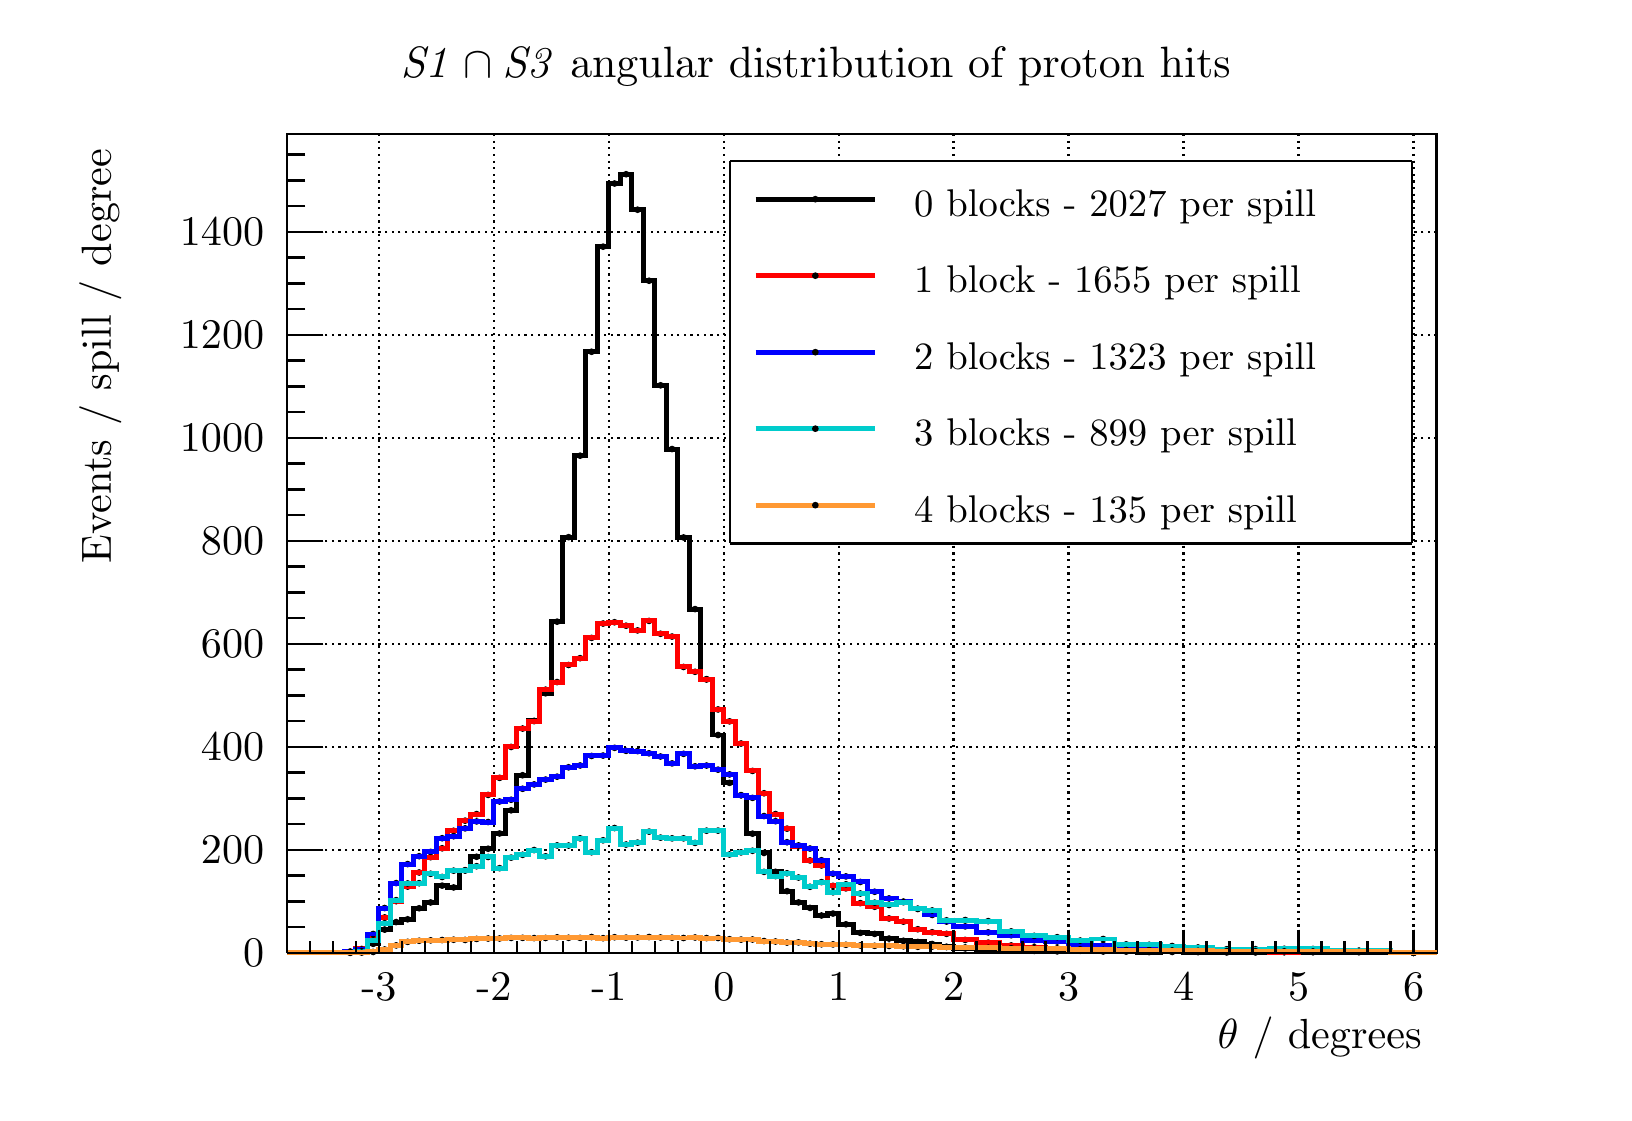
\begin{tikzpicture}
\pgfdeclareplotmark{cross} {
\pgfpathmoveto{\pgfpoint{-0.3\pgfplotmarksize}{\pgfplotmarksize}}
\pgfpathlineto{\pgfpoint{+0.3\pgfplotmarksize}{\pgfplotmarksize}}
\pgfpathlineto{\pgfpoint{+0.3\pgfplotmarksize}{0.3\pgfplotmarksize}}
\pgfpathlineto{\pgfpoint{+1\pgfplotmarksize}{0.3\pgfplotmarksize}}
\pgfpathlineto{\pgfpoint{+1\pgfplotmarksize}{-0.3\pgfplotmarksize}}
\pgfpathlineto{\pgfpoint{+0.3\pgfplotmarksize}{-0.3\pgfplotmarksize}}
\pgfpathlineto{\pgfpoint{+0.3\pgfplotmarksize}{-1.\pgfplotmarksize}}
\pgfpathlineto{\pgfpoint{-0.3\pgfplotmarksize}{-1.\pgfplotmarksize}}
\pgfpathlineto{\pgfpoint{-0.3\pgfplotmarksize}{-0.3\pgfplotmarksize}}
\pgfpathlineto{\pgfpoint{-1.\pgfplotmarksize}{-0.3\pgfplotmarksize}}
\pgfpathlineto{\pgfpoint{-1.\pgfplotmarksize}{0.3\pgfplotmarksize}}
\pgfpathlineto{\pgfpoint{-0.3\pgfplotmarksize}{0.3\pgfplotmarksize}}
\pgfpathclose
\pgfusepathqstroke
}
\pgfdeclareplotmark{cross*} {
\pgfpathmoveto{\pgfpoint{-0.3\pgfplotmarksize}{\pgfplotmarksize}}
\pgfpathlineto{\pgfpoint{+0.3\pgfplotmarksize}{\pgfplotmarksize}}
\pgfpathlineto{\pgfpoint{+0.3\pgfplotmarksize}{0.3\pgfplotmarksize}}
\pgfpathlineto{\pgfpoint{+1\pgfplotmarksize}{0.3\pgfplotmarksize}}
\pgfpathlineto{\pgfpoint{+1\pgfplotmarksize}{-0.3\pgfplotmarksize}}
\pgfpathlineto{\pgfpoint{+0.3\pgfplotmarksize}{-0.3\pgfplotmarksize}}
\pgfpathlineto{\pgfpoint{+0.3\pgfplotmarksize}{-1.\pgfplotmarksize}}
\pgfpathlineto{\pgfpoint{-0.3\pgfplotmarksize}{-1.\pgfplotmarksize}}
\pgfpathlineto{\pgfpoint{-0.3\pgfplotmarksize}{-0.3\pgfplotmarksize}}
\pgfpathlineto{\pgfpoint{-1.\pgfplotmarksize}{-0.3\pgfplotmarksize}}
\pgfpathlineto{\pgfpoint{-1.\pgfplotmarksize}{0.3\pgfplotmarksize}}
\pgfpathlineto{\pgfpoint{-0.3\pgfplotmarksize}{0.3\pgfplotmarksize}}
\pgfpathclose
\pgfusepathqfillstroke
}
\pgfdeclareplotmark{newstar} {
\pgfpathmoveto{\pgfqpoint{0pt}{\pgfplotmarksize}}
\pgfpathlineto{\pgfqpointpolar{44}{0.5\pgfplotmarksize}}
\pgfpathlineto{\pgfqpointpolar{18}{\pgfplotmarksize}}
\pgfpathlineto{\pgfqpointpolar{-20}{0.5\pgfplotmarksize}}
\pgfpathlineto{\pgfqpointpolar{-54}{\pgfplotmarksize}}
\pgfpathlineto{\pgfqpointpolar{-90}{0.5\pgfplotmarksize}}
\pgfpathlineto{\pgfqpointpolar{234}{\pgfplotmarksize}}
\pgfpathlineto{\pgfqpointpolar{198}{0.5\pgfplotmarksize}}
\pgfpathlineto{\pgfqpointpolar{162}{\pgfplotmarksize}}
\pgfpathlineto{\pgfqpointpolar{134}{0.5\pgfplotmarksize}}
\pgfpathclose
\pgfusepathqstroke
}
\pgfdeclareplotmark{newstar*} {
\pgfpathmoveto{\pgfqpoint{0pt}{\pgfplotmarksize}}
\pgfpathlineto{\pgfqpointpolar{44}{0.5\pgfplotmarksize}}
\pgfpathlineto{\pgfqpointpolar{18}{\pgfplotmarksize}}
\pgfpathlineto{\pgfqpointpolar{-20}{0.5\pgfplotmarksize}}
\pgfpathlineto{\pgfqpointpolar{-54}{\pgfplotmarksize}}
\pgfpathlineto{\pgfqpointpolar{-90}{0.5\pgfplotmarksize}}
\pgfpathlineto{\pgfqpointpolar{234}{\pgfplotmarksize}}
\pgfpathlineto{\pgfqpointpolar{198}{0.5\pgfplotmarksize}}
\pgfpathlineto{\pgfqpointpolar{162}{\pgfplotmarksize}}
\pgfpathlineto{\pgfqpointpolar{134}{0.5\pgfplotmarksize}}
\pgfpathclose
\pgfusepathqfillstroke
}
\definecolor{c}{rgb}{1,1,1};
\draw [color=c, fill=c] (0,0) rectangle (20,13.5143);
\draw [color=c, fill=c] (3.28571,1.77143) rectangle (17.8857,12.1714);
\definecolor{c}{rgb}{0,0,0};
\draw [c,line width=0.9] (3.28571,1.77143) -- (3.28571,12.1714) -- (17.8857,12.1714) -- (17.8857,1.77143) -- (3.28571,1.77143);
\definecolor{c}{rgb}{1,1,1};
\draw [color=c, fill=c] (3.28571,1.77143) rectangle (17.8857,12.1714);
\definecolor{c}{rgb}{0,0,0};
\draw [c,line width=0.9] (3.28571,1.77143) -- (3.28571,12.1714) -- (17.8857,12.1714) -- (17.8857,1.77143) -- (3.28571,1.77143);
\draw [c,line width=0.9] (3.28571,1.77143) -- (17.8857,1.77143);
\draw [c,dash pattern=on 0.80pt off 1.60pt ,line width=0.9] (4.45371,12.1714) -- (4.45371,1.77143);
\draw [c,dash pattern=on 0.80pt off 1.60pt ,line width=0.9] (5.91371,12.1714) -- (5.91371,1.77143);
\draw [c,dash pattern=on 0.80pt off 1.60pt ,line width=0.9] (7.37371,12.1714) -- (7.37371,1.77143);
\draw [c,dash pattern=on 0.80pt off 1.60pt ,line width=0.9] (8.83371,12.1714) -- (8.83371,1.77143);
\draw [c,dash pattern=on 0.80pt off 1.60pt ,line width=0.9] (10.2937,12.1714) -- (10.2937,1.77143);
\draw [c,dash pattern=on 0.80pt off 1.60pt ,line width=0.9] (11.7537,12.1714) -- (11.7537,1.77143);
\draw [c,dash pattern=on 0.80pt off 1.60pt ,line width=0.9] (13.2137,12.1714) -- (13.2137,1.77143);
\draw [c,dash pattern=on 0.80pt off 1.60pt ,line width=0.9] (14.6737,12.1714) -- (14.6737,1.77143);
\draw [c,dash pattern=on 0.80pt off 1.60pt ,line width=0.9] (16.1337,12.1714) -- (16.1337,1.77143);
\draw [c,dash pattern=on 0.80pt off 1.60pt ,line width=0.9] (17.5937,12.1714) -- (17.5937,1.77143);
\draw [c,dash pattern=on 0.80pt off 1.60pt ,line width=0.9] (4.45371,12.1714) -- (4.45371,1.77143);
\draw [c,dash pattern=on 0.80pt off 1.60pt ,line width=0.9] (17.5937,12.1714) -- (17.5937,1.77143);
\draw [c,line width=0.9] (3.28571,1.77143) -- (3.28571,12.1714);
\draw [c,dash pattern=on 0.80pt off 1.60pt ,line width=0.9] (17.8857,1.77143) -- (3.28571,1.77143);
\draw [c,dash pattern=on 0.80pt off 1.60pt ,line width=0.9] (17.8857,3.07955) -- (3.28571,3.07955);
\draw [c,dash pattern=on 0.80pt off 1.60pt ,line width=0.9] (17.8857,4.38766) -- (3.28571,4.38766);
\draw [c,dash pattern=on 0.80pt off 1.60pt ,line width=0.9] (17.8857,5.69578) -- (3.28571,5.69578);
\draw [c,dash pattern=on 0.80pt off 1.60pt ,line width=0.9] (17.8857,7.0039) -- (3.28571,7.0039);
\draw [c,dash pattern=on 0.80pt off 1.60pt ,line width=0.9] (17.8857,8.31201) -- (3.28571,8.31201);
\draw [c,dash pattern=on 0.80pt off 1.60pt ,line width=0.9] (17.8857,9.62013) -- (3.28571,9.62013);
\draw [c,dash pattern=on 0.80pt off 1.60pt ,line width=0.9] (17.8857,10.9282) -- (3.28571,10.9282);
\draw [c,dash pattern=on 0.80pt off 1.60pt ,line width=0.9] (17.8857,10.9282) -- (3.28571,10.9282);
\definecolor{c}{rgb}{0,0,0.6};
\draw [c,line width=0.9] (3.28571,1.77143) -- (3.43171,1.77143) -- (3.43171,1.77143) -- (3.57771,1.77143) -- (3.57771,1.77143) -- (3.72371,1.77143) -- (3.72371,1.77143) -- (3.86971,1.77143) -- (3.86971,1.77143) -- (4.01571,1.77143) --
 (4.01571,1.77143) -- (4.16171,1.77143) -- (4.16171,1.77143) -- (4.30771,1.77143) -- (4.30771,1.77143) -- (4.45371,1.77143) -- (4.45371,1.77143) -- (4.59971,1.77143) -- (4.59971,1.77143) -- (4.74571,1.77143) -- (4.74571,1.77143) -- (4.89171,1.77143)
 -- (4.89171,1.77143) -- (5.03771,1.77143) -- (5.03771,1.77143) -- (5.18371,1.77143) -- (5.18371,1.77143) -- (5.32971,1.77143) -- (5.32971,1.77143) -- (5.47571,1.77143) -- (5.47571,1.77143) -- (5.62171,1.77143) -- (5.62171,1.77143) --
 (5.76771,1.77143) -- (5.76771,1.77143) -- (5.91371,1.77143) -- (5.91371,1.77143) -- (6.05971,1.77143) -- (6.05971,1.77143) -- (6.20571,1.77143) -- (6.20571,1.77143) -- (6.35171,1.77143) -- (6.35171,1.77143) -- (6.49771,1.77143) -- (6.49771,1.77143)
 -- (6.64371,1.77143) -- (6.64371,1.77143) -- (6.78971,1.77143) -- (6.78971,1.77143) -- (6.93571,1.77143) -- (6.93571,1.77143) -- (7.08171,1.77143) -- (7.08171,1.77143) -- (7.22771,1.77143) -- (7.22771,1.77143) -- (7.37371,1.77143) --
 (7.37371,1.77143) -- (7.51971,1.77143) -- (7.51971,1.77143) -- (7.66571,1.77143) -- (7.66571,1.77143) -- (7.81171,1.77143) -- (7.81171,1.77143) -- (7.95771,1.77143) -- (7.95771,1.77143) -- (8.10371,1.77143) -- (8.10371,1.77143) -- (8.24971,1.77143)
 -- (8.24971,1.77143) -- (8.39571,1.77143) -- (8.39571,1.77143) -- (8.54171,1.77143) -- (8.54171,1.77143) -- (8.68771,1.77143) -- (8.68771,1.77143) -- (8.83371,1.77143) -- (8.83371,1.77143) -- (8.97971,1.77143) -- (8.97971,1.77143) --
 (9.12571,1.77143) -- (9.12571,1.77143) -- (9.27171,1.77143) -- (9.27171,1.77143) -- (9.41771,1.77143) -- (9.41771,1.77143) -- (9.56371,1.77143) -- (9.56371,1.77143) -- (9.70971,1.77143) -- (9.70971,1.77143) -- (9.85571,1.77143) -- (9.85571,1.77143)
 -- (10.0017,1.77143) -- (10.0017,1.77143) -- (10.1477,1.77143) -- (10.1477,1.77143) -- (10.2937,1.77143) -- (10.2937,1.77143) -- (10.4762,1.77143) -- (10.4762,1.77143) -- (10.6587,1.77143) -- (10.6587,1.77143) -- (10.8412,1.77143) --
 (10.8412,1.77143) -- (11.0237,1.77143) -- (11.0237,1.77143) -- (11.2062,1.77143) -- (11.2062,1.77143) -- (11.3887,1.77143) -- (11.3887,1.77143) -- (11.5712,1.77143) -- (11.5712,1.77143) -- (11.7537,1.77143) -- (11.7537,1.77143) -- (12.0457,1.77143)
 -- (12.0457,1.77143) -- (12.3377,1.77143) -- (12.3377,1.77143) -- (12.6297,1.77143) -- (12.6297,1.77143) -- (12.9217,1.77143) -- (12.9217,1.77143) -- (13.2137,1.77143) -- (13.2137,1.77143) -- (13.5057,1.77143) -- (13.5057,1.77143) --
 (13.7977,1.77143) -- (13.7977,1.77143) -- (14.0897,1.77143) -- (14.0897,1.77143) -- (14.3817,1.77143) -- (14.3817,1.77143) -- (14.6737,1.77143) -- (14.6737,1.77143) -- (15.0387,1.77143) -- (15.0387,1.77143) -- (15.4037,1.77143) -- (15.4037,1.77143)
 -- (15.7687,1.77143) -- (15.7687,1.77143) -- (16.1337,1.77143) -- (16.1337,1.77143) -- (16.4987,1.77143) -- (16.4987,1.77143) -- (17.3017,1.77143) -- (17.3017,1.77143) -- (17.8857,1.77143);
\definecolor{c}{rgb}{0,0,0};
\draw [c,line width=0.9] (3.28571,1.77143) -- (17.8857,1.77143);
\draw [c,line width=0.9] (4.45371,2.06739) -- (4.45371,1.77143);
\draw [c,line width=0.9] (4.74571,1.91941) -- (4.74571,1.77143);
\draw [c,line width=0.9] (5.03771,1.91941) -- (5.03771,1.77143);
\draw [c,line width=0.9] (5.32971,1.91941) -- (5.32971,1.77143);
\draw [c,line width=0.9] (5.62171,1.91941) -- (5.62171,1.77143);
\draw [c,line width=0.9] (5.91371,2.06739) -- (5.91371,1.77143);
\draw [c,line width=0.9] (6.20571,1.91941) -- (6.20571,1.77143);
\draw [c,line width=0.9] (6.49771,1.91941) -- (6.49771,1.77143);
\draw [c,line width=0.9] (6.78971,1.91941) -- (6.78971,1.77143);
\draw [c,line width=0.9] (7.08171,1.91941) -- (7.08171,1.77143);
\draw [c,line width=0.9] (7.37371,2.06739) -- (7.37371,1.77143);
\draw [c,line width=0.9] (7.66571,1.91941) -- (7.66571,1.77143);
\draw [c,line width=0.9] (7.95771,1.91941) -- (7.95771,1.77143);
\draw [c,line width=0.9] (8.24971,1.91941) -- (8.24971,1.77143);
\draw [c,line width=0.9] (8.54171,1.91941) -- (8.54171,1.77143);
\draw [c,line width=0.9] (8.83371,2.06739) -- (8.83371,1.77143);
\draw [c,line width=0.9] (9.12571,1.91941) -- (9.12571,1.77143);
\draw [c,line width=0.9] (9.41771,1.91941) -- (9.41771,1.77143);
\draw [c,line width=0.9] (9.70971,1.91941) -- (9.70971,1.77143);
\draw [c,line width=0.9] (10.0017,1.91941) -- (10.0017,1.77143);
\draw [c,line width=0.9] (10.2937,2.06739) -- (10.2937,1.77143);
\draw [c,line width=0.9] (10.5857,1.91941) -- (10.5857,1.77143);
\draw [c,line width=0.9] (10.8777,1.91941) -- (10.8777,1.77143);
\draw [c,line width=0.9] (11.1697,1.91941) -- (11.1697,1.77143);
\draw [c,line width=0.9] (11.4617,1.91941) -- (11.4617,1.77143);
\draw [c,line width=0.9] (11.7537,2.06739) -- (11.7537,1.77143);
\draw [c,line width=0.9] (12.0457,1.91941) -- (12.0457,1.77143);
\draw [c,line width=0.9] (12.3377,1.91941) -- (12.3377,1.77143);
\draw [c,line width=0.9] (12.6297,1.91941) -- (12.6297,1.77143);
\draw [c,line width=0.9] (12.9217,1.91941) -- (12.9217,1.77143);
\draw [c,line width=0.9] (13.2137,2.06739) -- (13.2137,1.77143);
\draw [c,line width=0.9] (13.5057,1.91941) -- (13.5057,1.77143);
\draw [c,line width=0.9] (13.7977,1.91941) -- (13.7977,1.77143);
\draw [c,line width=0.9] (14.0897,1.91941) -- (14.0897,1.77143);
\draw [c,line width=0.9] (14.3817,1.91941) -- (14.3817,1.77143);
\draw [c,line width=0.9] (14.6737,2.06739) -- (14.6737,1.77143);
\draw [c,line width=0.9] (14.9657,1.91941) -- (14.9657,1.77143);
\draw [c,line width=0.9] (15.2577,1.91941) -- (15.2577,1.77143);
\draw [c,line width=0.9] (15.5497,1.91941) -- (15.5497,1.77143);
\draw [c,line width=0.9] (15.8417,1.91941) -- (15.8417,1.77143);
\draw [c,line width=0.9] (16.1337,2.06739) -- (16.1337,1.77143);
\draw [c,line width=0.9] (16.4257,1.91941) -- (16.4257,1.77143);
\draw [c,line width=0.9] (16.7177,1.91941) -- (16.7177,1.77143);
\draw [c,line width=0.9] (17.0097,1.91941) -- (17.0097,1.77143);
\draw [c,line width=0.9] (17.3017,1.91941) -- (17.3017,1.77143);
\draw [c,line width=0.9] (17.5937,2.06739) -- (17.5937,1.77143);
\draw [c,line width=0.9] (4.45371,2.06739) -- (4.45371,1.77143);
\draw [c,line width=0.9] (4.16171,1.91941) -- (4.16171,1.77143);
\draw [c,line width=0.9] (3.86971,1.91941) -- (3.86971,1.77143);
\draw [c,line width=0.9] (3.57771,1.91941) -- (3.57771,1.77143);
\draw [c,line width=0.9] (17.5937,2.06739) -- (17.5937,1.77143);
\draw [anchor=base] (4.45371,1.16329) node[scale=1.52295, color=c, rotate=0]{-3};
\draw [anchor=base] (5.91371,1.16329) node[scale=1.52295, color=c, rotate=0]{-2};
\draw [anchor=base] (7.37371,1.16329) node[scale=1.52295, color=c, rotate=0]{-1};
\draw [anchor=base] (8.83371,1.16329) node[scale=1.52295, color=c, rotate=0]{0};
\draw [anchor=base] (10.2937,1.16329) node[scale=1.52295, color=c, rotate=0]{1};
\draw [anchor=base] (11.7537,1.16329) node[scale=1.52295, color=c, rotate=0]{2};
\draw [anchor=base] (13.2137,1.16329) node[scale=1.52295, color=c, rotate=0]{3};
\draw [anchor=base] (14.6737,1.16329) node[scale=1.52295, color=c, rotate=0]{4};
\draw [anchor=base] (16.1337,1.16329) node[scale=1.52295, color=c, rotate=0]{5};
\draw [anchor=base] (17.5937,1.16329) node[scale=1.52295, color=c, rotate=0]{6};
\draw [anchor= east] (17.8857,0.690286) node[scale=1.52295, color=c, rotate=0]{$\theta$ / degrees};
\draw [c,line width=0.9] (3.28571,1.77143) -- (3.28571,12.1714);
\draw [c,line width=0.9] (3.74745,1.77143) -- (3.28571,1.77143);
\draw [c,line width=0.9] (3.51658,2.09846) -- (3.28571,2.09846);
\draw [c,line width=0.9] (3.51658,2.42549) -- (3.28571,2.42549);
\draw [c,line width=0.9] (3.51658,2.75252) -- (3.28571,2.75252);
\draw [c,line width=0.9] (3.74745,3.07955) -- (3.28571,3.07955);
\draw [c,line width=0.9] (3.51658,3.40658) -- (3.28571,3.40658);
\draw [c,line width=0.9] (3.51658,3.7336) -- (3.28571,3.7336);
\draw [c,line width=0.9] (3.51658,4.06063) -- (3.28571,4.06063);
\draw [c,line width=0.9] (3.74745,4.38766) -- (3.28571,4.38766);
\draw [c,line width=0.9] (3.51658,4.71469) -- (3.28571,4.71469);
\draw [c,line width=0.9] (3.51658,5.04172) -- (3.28571,5.04172);
\draw [c,line width=0.9] (3.51658,5.36875) -- (3.28571,5.36875);
\draw [c,line width=0.9] (3.74745,5.69578) -- (3.28571,5.69578);
\draw [c,line width=0.9] (3.51658,6.02281) -- (3.28571,6.02281);
\draw [c,line width=0.9] (3.51658,6.34984) -- (3.28571,6.34984);
\draw [c,line width=0.9] (3.51658,6.67687) -- (3.28571,6.67687);
\draw [c,line width=0.9] (3.74745,7.0039) -- (3.28571,7.0039);
\draw [c,line width=0.9] (3.51658,7.33093) -- (3.28571,7.33093);
\draw [c,line width=0.9] (3.51658,7.65796) -- (3.28571,7.65796);
\draw [c,line width=0.9] (3.51658,7.98499) -- (3.28571,7.98499);
\draw [c,line width=0.9] (3.74745,8.31201) -- (3.28571,8.31201);
\draw [c,line width=0.9] (3.51658,8.63904) -- (3.28571,8.63904);
\draw [c,line width=0.9] (3.51658,8.96607) -- (3.28571,8.96607);
\draw [c,line width=0.9] (3.51658,9.2931) -- (3.28571,9.2931);
\draw [c,line width=0.9] (3.74745,9.62013) -- (3.28571,9.62013);
\draw [c,line width=0.9] (3.51658,9.94716) -- (3.28571,9.94716);
\draw [c,line width=0.9] (3.51658,10.2742) -- (3.28571,10.2742);
\draw [c,line width=0.9] (3.51658,10.6012) -- (3.28571,10.6012);
\draw [c,line width=0.9] (3.74745,10.9282) -- (3.28571,10.9282);
\draw [c,line width=0.9] (3.74745,10.9282) -- (3.28571,10.9282);
\draw [c,line width=0.9] (3.51658,11.2553) -- (3.28571,11.2553);
\draw [c,line width=0.9] (3.51658,11.5823) -- (3.28571,11.5823);
\draw [c,line width=0.9] (3.51658,11.9093) -- (3.28571,11.9093);
\draw [anchor= east] (3.18571,1.77143) node[scale=1.52295, color=c, rotate=0]{0};
\draw [anchor= east] (3.18571,3.07955) node[scale=1.52295, color=c, rotate=0]{200};
\draw [anchor= east] (3.18571,4.38766) node[scale=1.52295, color=c, rotate=0]{400};
\draw [anchor= east] (3.18571,5.69578) node[scale=1.52295, color=c, rotate=0]{600};
\draw [anchor= east] (3.18571,7.0039) node[scale=1.52295, color=c, rotate=0]{800};
\draw [anchor= east] (3.18571,8.31201) node[scale=1.52295, color=c, rotate=0]{1000};
\draw [anchor= east] (3.18571,9.62013) node[scale=1.52295, color=c, rotate=0]{1200};
\draw [anchor= east] (3.18571,10.9282) node[scale=1.52295, color=c, rotate=0]{1400};
\draw [anchor= east] (0.914286,12.1714) node[scale=1.52295, color=c, rotate=90]{ Events / spill / degree};
\draw [c,line width=1.8] (4.08871,1.77928) -- (4.08871,1.77976);
\draw [c,line width=1.8] (4.08871,1.77976) -- (4.08871,1.78025);
\foreach \P in {(4.08871,1.77976)}{\draw[mark options={color=c,fill=c},mark size=2.402402pt,mark=*,mark size=1pt] plot coordinates {\P};}
\draw [c,line width=1.8] (4.23471,1.80702) -- (4.23471,1.808);
\draw [c,line width=1.8] (4.23471,1.808) -- (4.23471,1.80898);
\foreach \P in {(4.23471,1.808)}{\draw[mark options={color=c,fill=c},mark size=2.402402pt,mark=*,mark size=1pt] plot coordinates {\P};}
\draw [c,line width=1.8] (4.38071,1.88391) -- (4.38071,1.88565);
\draw [c,line width=1.8] (4.38071,1.88565) -- (4.38071,1.88738);
\foreach \P in {(4.38071,1.88565)}{\draw[mark options={color=c,fill=c},mark size=2.402402pt,mark=*,mark size=1pt] plot coordinates {\P};}
\draw [c,line width=1.8] (4.52671,2.0637) -- (4.52671,2.0665);
\draw [c,line width=1.8] (4.52671,2.0665) -- (4.52671,2.0693);
\foreach \P in {(4.52671,2.0665)}{\draw[mark options={color=c,fill=c},mark size=2.402402pt,mark=*,mark size=1pt] plot coordinates {\P};}
\draw [c,line width=1.8] (4.67271,2.15927) -- (4.67271,2.16245);
\draw [c,line width=1.8] (4.67271,2.16245) -- (4.67271,2.16564);
\foreach \P in {(4.67271,2.16245)}{\draw[mark options={color=c,fill=c},mark size=2.402402pt,mark=*,mark size=1pt] plot coordinates {\P};}
\draw [c,line width=1.8] (4.81871,2.19429) -- (4.81871,2.19763);
\draw [c,line width=1.8] (4.81871,2.19763) -- (4.81871,2.20096);
\foreach \P in {(4.81871,2.19763)}{\draw[mark options={color=c,fill=c},mark size=2.402402pt,mark=*,mark size=1pt] plot coordinates {\P};}
\draw [c,line width=1.8] (4.96471,2.33421) -- (4.96471,2.33808);
\draw [c,line width=1.8] (4.96471,2.33808) -- (4.96471,2.34194);
\foreach \P in {(4.96471,2.33808)}{\draw[mark options={color=c,fill=c},mark size=2.402402pt,mark=*,mark size=1pt] plot coordinates {\P};}
\draw [c,line width=1.8] (5.11071,2.40725) -- (5.11071,2.41137);
\draw [c,line width=1.8] (5.11071,2.41137) -- (5.11071,2.41549);
\foreach \P in {(5.11071,2.41137)}{\draw[mark options={color=c,fill=c},mark size=2.402402pt,mark=*,mark size=1pt] plot coordinates {\P};}
\draw [c,line width=1.8] (5.25671,2.62065) -- (5.25671,2.62539);
\draw [c,line width=1.8] (5.25671,2.62539) -- (5.25671,2.63013);
\foreach \P in {(5.25671,2.62539)}{\draw[mark options={color=c,fill=c},mark size=2.402402pt,mark=*,mark size=1pt] plot coordinates {\P};}
\draw [c,line width=1.8] (5.40271,2.5977) -- (5.40271,2.60239);
\draw [c,line width=1.8] (5.40271,2.60239) -- (5.40271,2.60707);
\foreach \P in {(5.40271,2.60239)}{\draw[mark options={color=c,fill=c},mark size=2.402402pt,mark=*,mark size=1pt] plot coordinates {\P};}
\draw [c,line width=1.8] (5.54871,2.8114) -- (5.54871,2.81666);
\draw [c,line width=1.8] (5.54871,2.81666) -- (5.54871,2.82192);
\foreach \P in {(5.54871,2.81666)}{\draw[mark options={color=c,fill=c},mark size=2.402402pt,mark=*,mark size=1pt] plot coordinates {\P};}
\draw [c,line width=1.8] (5.69471,2.9861) -- (5.69471,2.99178);
\draw [c,line width=1.8] (5.69471,2.99178) -- (5.69471,2.99746);
\foreach \P in {(5.69471,2.99178)}{\draw[mark options={color=c,fill=c},mark size=2.402402pt,mark=*,mark size=1pt] plot coordinates {\P};}
\draw [c,line width=1.8] (5.84071,3.08772) -- (5.84071,3.09363);
\draw [c,line width=1.8] (5.84071,3.09363) -- (5.84071,3.09954);
\foreach \P in {(5.84071,3.09363)}{\draw[mark options={color=c,fill=c},mark size=2.402402pt,mark=*,mark size=1pt] plot coordinates {\P};}
\draw [c,line width=1.8] (5.98671,3.28119) -- (5.98671,3.28753);
\draw [c,line width=1.8] (5.98671,3.28753) -- (5.98671,3.29387);
\foreach \P in {(5.98671,3.28753)}{\draw[mark options={color=c,fill=c},mark size=2.402402pt,mark=*,mark size=1pt] plot coordinates {\P};}
\draw [c,line width=1.8] (6.13271,3.57494) -- (6.13271,3.58187);
\draw [c,line width=1.8] (6.13271,3.58187) -- (6.13271,3.58879);
\foreach \P in {(6.13271,3.58187)}{\draw[mark options={color=c,fill=c},mark size=2.402402pt,mark=*,mark size=1pt] plot coordinates {\P};}
\draw [c,line width=1.8] (6.27871,4.01937) -- (6.27871,4.02712);
\draw [c,line width=1.8] (6.27871,4.02712) -- (6.27871,4.03486);
\foreach \P in {(6.27871,4.02712)}{\draw[mark options={color=c,fill=c},mark size=2.402402pt,mark=*,mark size=1pt] plot coordinates {\P};}
\draw [c,line width=1.8] (6.42471,4.70892) -- (6.42471,4.71772);
\draw [c,line width=1.8] (6.42471,4.71772) -- (6.42471,4.72652);
\foreach \P in {(6.42471,4.71772)}{\draw[mark options={color=c,fill=c},mark size=2.402402pt,mark=*,mark size=1pt] plot coordinates {\P};}
\draw [c,line width=1.8] (6.57071,5.05873) -- (6.57071,5.06808);
\draw [c,line width=1.8] (6.57071,5.06808) -- (6.57071,5.07743);
\foreach \P in {(6.57071,5.06808)}{\draw[mark options={color=c,fill=c},mark size=2.402402pt,mark=*,mark size=1pt] plot coordinates {\P};}
\draw [c,line width=1.8] (6.71671,5.96677) -- (6.71671,5.9773);
\draw [c,line width=1.8] (6.71671,5.9773) -- (6.71671,5.98784);
\foreach \P in {(6.71671,5.9773)}{\draw[mark options={color=c,fill=c},mark size=2.402402pt,mark=*,mark size=1pt] plot coordinates {\P};}
\draw [c,line width=1.8] (6.86271,7.03879) -- (6.86271,7.05058);
\draw [c,line width=1.8] (6.86271,7.05058) -- (6.86271,7.06238);
\foreach \P in {(6.86271,7.05058)}{\draw[mark options={color=c,fill=c},mark size=2.402402pt,mark=*,mark size=1pt] plot coordinates {\P};}
\draw [c,line width=1.8] (7.00871,8.07255) -- (7.00871,8.08548);
\draw [c,line width=1.8] (7.00871,8.08548) -- (7.00871,8.09841);
\foreach \P in {(7.00871,8.08548)}{\draw[mark options={color=c,fill=c},mark size=2.402402pt,mark=*,mark size=1pt] plot coordinates {\P};}
\draw [c,line width=1.8] (7.15471,9.39111) -- (7.15471,9.40531);
\draw [c,line width=1.8] (7.15471,9.40531) -- (7.15471,9.41952);
\foreach \P in {(7.15471,9.40531)}{\draw[mark options={color=c,fill=c},mark size=2.402402pt,mark=*,mark size=1pt] plot coordinates {\P};}
\draw [c,line width=1.8] (7.30071,10.7244) -- (7.30071,10.7398);
\draw [c,line width=1.8] (7.30071,10.7398) -- (7.30071,10.7552);
\foreach \P in {(7.30071,10.7398)}{\draw[mark options={color=c,fill=c},mark size=2.402402pt,mark=*,mark size=1pt] plot coordinates {\P};}
\draw [c,line width=1.8] (7.44671,11.5259) -- (7.44671,11.542);
\draw [c,line width=1.8] (7.44671,11.542) -- (7.44671,11.5581);
\foreach \P in {(7.44671,11.542)}{\draw[mark options={color=c,fill=c},mark size=2.402402pt,mark=*,mark size=1pt] plot coordinates {\P};}
\draw [c,line width=1.8] (7.59271,11.6439) -- (7.59271,11.66);
\draw [c,line width=1.8] (7.59271,11.66) -- (7.59271,11.6762);
\foreach \P in {(7.59271,11.66)}{\draw[mark options={color=c,fill=c},mark size=2.402402pt,mark=*,mark size=1pt] plot coordinates {\P};}
\draw [c,line width=1.8] (7.73871,11.1933) -- (7.73871,11.2091);
\draw [c,line width=1.8] (7.73871,11.2091) -- (7.73871,11.2249);
\foreach \P in {(7.73871,11.2091)}{\draw[mark options={color=c,fill=c},mark size=2.402402pt,mark=*,mark size=1pt] plot coordinates {\P};}
\draw [c,line width=1.8] (7.88471,10.292) -- (7.88471,10.307);
\draw [c,line width=1.8] (7.88471,10.307) -- (7.88471,10.322);
\foreach \P in {(7.88471,10.307)}{\draw[mark options={color=c,fill=c},mark size=2.402402pt,mark=*,mark size=1pt] plot coordinates {\P};}
\draw [c,line width=1.8] (8.03071,8.96539) -- (8.03071,8.97916);
\draw [c,line width=1.8] (8.03071,8.97916) -- (8.03071,8.99293);
\foreach \P in {(8.03071,8.97916)}{\draw[mark options={color=c,fill=c},mark size=2.402402pt,mark=*,mark size=1pt] plot coordinates {\P};}
\draw [c,line width=1.8] (8.17671,8.15671) -- (8.17671,8.1697);
\draw [c,line width=1.8] (8.17671,8.1697) -- (8.17671,8.18269);
\foreach \P in {(8.17671,8.1697)}{\draw[mark options={color=c,fill=c},mark size=2.402402pt,mark=*,mark size=1pt] plot coordinates {\P};}
\draw [c,line width=1.8] (8.32271,7.03519) -- (8.32271,7.04698);
\draw [c,line width=1.8] (8.32271,7.04698) -- (8.32271,7.05876);
\foreach \P in {(8.32271,7.04698)}{\draw[mark options={color=c,fill=c},mark size=2.402402pt,mark=*,mark size=1pt] plot coordinates {\P};}
\draw [c,line width=1.8] (8.46871,6.12634) -- (8.46871,6.13709);
\draw [c,line width=1.8] (8.46871,6.13709) -- (8.46871,6.14784);
\foreach \P in {(8.46871,6.13709)}{\draw[mark options={color=c,fill=c},mark size=2.402402pt,mark=*,mark size=1pt] plot coordinates {\P};}
\draw [c,line width=1.8] (8.61471,5.23363) -- (8.61471,5.24318);
\draw [c,line width=1.8] (8.61471,5.24318) -- (8.61471,5.25272);
\foreach \P in {(8.61471,5.24318)}{\draw[mark options={color=c,fill=c},mark size=2.402402pt,mark=*,mark size=1pt] plot coordinates {\P};}
\draw [c,line width=1.8] (8.76071,4.52978) -- (8.76071,4.53832);
\draw [c,line width=1.8] (8.76071,4.53832) -- (8.76071,4.54686);
\foreach \P in {(8.76071,4.53832)}{\draw[mark options={color=c,fill=c},mark size=2.402402pt,mark=*,mark size=1pt] plot coordinates {\P};}
\draw [c,line width=1.8] (8.90671,3.9228) -- (8.90671,3.93034);
\draw [c,line width=1.8] (8.90671,3.93034) -- (8.90671,3.93787);
\foreach \P in {(8.90671,3.93034)}{\draw[mark options={color=c,fill=c},mark size=2.402402pt,mark=*,mark size=1pt] plot coordinates {\P};}
\draw [c,line width=1.8] (9.05271,3.76622) -- (9.05271,3.77346);
\draw [c,line width=1.8] (9.05271,3.77346) -- (9.05271,3.7807);
\foreach \P in {(9.05271,3.77346)}{\draw[mark options={color=c,fill=c},mark size=2.402402pt,mark=*,mark size=1pt] plot coordinates {\P};}
\draw [c,line width=1.8] (9.19871,3.27871) -- (9.19871,3.28503);
\draw [c,line width=1.8] (9.19871,3.28503) -- (9.19871,3.29134);
\foreach \P in {(9.19871,3.28503)}{\draw[mark options={color=c,fill=c},mark size=2.402402pt,mark=*,mark size=1pt] plot coordinates {\P};}
\draw [c,line width=1.8] (9.34471,3.0343) -- (9.34471,3.0401);
\draw [c,line width=1.8] (9.34471,3.0401) -- (9.34471,3.04591);
\foreach \P in {(9.34471,3.0401)}{\draw[mark options={color=c,fill=c},mark size=2.402402pt,mark=*,mark size=1pt] plot coordinates {\P};}
\draw [c,line width=1.8] (9.49071,2.7953) -- (9.49071,2.8005);
\draw [c,line width=1.8] (9.49071,2.8005) -- (9.49071,2.8057);
\foreach \P in {(9.49071,2.8005)}{\draw[mark options={color=c,fill=c},mark size=2.402402pt,mark=*,mark size=1pt] plot coordinates {\P};}
\draw [c,line width=1.8] (9.63671,2.55056) -- (9.63671,2.55512);
\draw [c,line width=1.8] (9.63671,2.55512) -- (9.63671,2.55967);
\foreach \P in {(9.63671,2.55512)}{\draw[mark options={color=c,fill=c},mark size=2.402402pt,mark=*,mark size=1pt] plot coordinates {\P};}
\draw [c,line width=1.8] (9.78271,2.40811) -- (9.78271,2.41224);
\draw [c,line width=1.8] (9.78271,2.41224) -- (9.78271,2.41636);
\foreach \P in {(9.78271,2.41224)}{\draw[mark options={color=c,fill=c},mark size=2.402402pt,mark=*,mark size=1pt] plot coordinates {\P};}
\draw [c,line width=1.8] (9.92871,2.33856) -- (9.92871,2.34245);
\draw [c,line width=1.8] (9.92871,2.34245) -- (9.92871,2.34633);
\foreach \P in {(9.92871,2.34245)}{\draw[mark options={color=c,fill=c},mark size=2.402402pt,mark=*,mark size=1pt] plot coordinates {\P};}
\draw [c,line width=1.8] (10.0747,2.24253) -- (10.0747,2.24605);
\draw [c,line width=1.8] (10.0747,2.24605) -- (10.0747,2.24957);
\foreach \P in {(10.0747,2.24605)}{\draw[mark options={color=c,fill=c},mark size=2.402402pt,mark=*,mark size=1pt] plot coordinates {\P};}
\draw [c,line width=1.8] (10.2207,2.26683) -- (10.2207,2.27048);
\draw [c,line width=1.8] (10.2207,2.27048) -- (10.2207,2.27413);
\foreach \P in {(10.2207,2.27048)}{\draw[mark options={color=c,fill=c},mark size=2.402402pt,mark=*,mark size=1pt] plot coordinates {\P};}
\draw [c,line width=1.8] (10.385,2.13071) -- (10.385,2.13417);
\draw [c,line width=1.8] (10.385,2.13417) -- (10.385,2.13762);
\foreach \P in {(10.385,2.13417)}{\draw[mark options={color=c,fill=c},mark size=2.402402pt,mark=*,mark size=1pt] plot coordinates {\P};}
\draw [c,line width=1.8] (10.5675,2.0223) -- (10.5675,2.02518);
\draw [c,line width=1.8] (10.5675,2.02518) -- (10.5675,2.02807);
\foreach \P in {(10.5675,2.02518)}{\draw[mark options={color=c,fill=c},mark size=2.402402pt,mark=*,mark size=1pt] plot coordinates {\P};}
\draw [c,line width=1.8] (10.75,2.0093) -- (10.75,2.01214);
\draw [c,line width=1.8] (10.75,2.01214) -- (10.75,2.01497);
\foreach \P in {(10.75,2.01214)}{\draw[mark options={color=c,fill=c},mark size=2.402402pt,mark=*,mark size=1pt] plot coordinates {\P};}
\draw [c,line width=1.8] (10.9325,1.95041) -- (10.9325,1.95285);
\draw [c,line width=1.8] (10.9325,1.95285) -- (10.9325,1.95529);
\foreach \P in {(10.9325,1.95285)}{\draw[mark options={color=c,fill=c},mark size=2.402402pt,mark=*,mark size=1pt] plot coordinates {\P};}
\draw [c,line width=1.8] (11.115,1.92247) -- (11.115,1.92473);
\draw [c,line width=1.8] (11.115,1.92473) -- (11.115,1.92699);
\foreach \P in {(11.115,1.92473)}{\draw[mark options={color=c,fill=c},mark size=2.402402pt,mark=*,mark size=1pt] plot coordinates {\P};}
\draw [c,line width=1.8] (11.2975,1.90792) -- (11.2975,1.91006);
\draw [c,line width=1.8] (11.2975,1.91006) -- (11.2975,1.9122);
\foreach \P in {(11.2975,1.91006)}{\draw[mark options={color=c,fill=c},mark size=2.402402pt,mark=*,mark size=1pt] plot coordinates {\P};}
\draw [c,line width=1.8] (11.48,1.88169) -- (11.48,1.88362);
\draw [c,line width=1.8] (11.48,1.88362) -- (11.48,1.88556);
\foreach \P in {(11.48,1.88362)}{\draw[mark options={color=c,fill=c},mark size=2.402402pt,mark=*,mark size=1pt] plot coordinates {\P};}
\draw [c,line width=1.8] (11.6625,1.84719) -- (11.6625,1.84877);
\draw [c,line width=1.8] (11.6625,1.84877) -- (11.6625,1.85034);
\foreach \P in {(11.6625,1.84877)}{\draw[mark options={color=c,fill=c},mark size=2.402402pt,mark=*,mark size=1pt] plot coordinates {\P};}
\draw [c,line width=1.8] (11.8997,1.8255) -- (11.8997,1.82722);
\draw [c,line width=1.8] (11.8997,1.82722) -- (11.8997,1.82893);
\foreach \P in {(11.8997,1.82722)}{\draw[mark options={color=c,fill=c},mark size=2.402402pt,mark=*,mark size=1pt] plot coordinates {\P};}
\draw [c,line width=1.8] (12.1917,1.80911) -- (12.1917,1.81054);
\draw [c,line width=1.8] (12.1917,1.81054) -- (12.1917,1.81198);
\foreach \P in {(12.1917,1.81054)}{\draw[mark options={color=c,fill=c},mark size=2.402402pt,mark=*,mark size=1pt] plot coordinates {\P};}
\draw [c,line width=1.8] (12.4837,1.80809) -- (12.4837,1.80951);
\draw [c,line width=1.8] (12.4837,1.80951) -- (12.4837,1.81093);
\foreach \P in {(12.4837,1.80951)}{\draw[mark options={color=c,fill=c},mark size=2.402402pt,mark=*,mark size=1pt] plot coordinates {\P};}
\draw [c,line width=1.8] (12.7757,1.79522) -- (12.7757,1.79637);
\draw [c,line width=1.8] (12.7757,1.79637) -- (12.7757,1.79753);
\foreach \P in {(12.7757,1.79637)}{\draw[mark options={color=c,fill=c},mark size=2.402402pt,mark=*,mark size=1pt] plot coordinates {\P};}
\draw [c,line width=1.8] (13.0677,1.78926) -- (13.0677,1.79027);
\draw [c,line width=1.8] (13.0677,1.79027) -- (13.0677,1.79128);
\foreach \P in {(13.0677,1.79027)}{\draw[mark options={color=c,fill=c},mark size=2.402402pt,mark=*,mark size=1pt] plot coordinates {\P};}
\draw [c,line width=1.8] (13.3597,1.7964) -- (13.3597,1.79758);
\draw [c,line width=1.8] (13.3597,1.79758) -- (13.3597,1.79876);
\foreach \P in {(13.3597,1.79758)}{\draw[mark options={color=c,fill=c},mark size=2.402402pt,mark=*,mark size=1pt] plot coordinates {\P};}
\draw [c,line width=1.8] (13.6517,1.78712) -- (13.6517,1.78804);
\draw [c,line width=1.8] (13.6517,1.78804) -- (13.6517,1.78897);
\foreach \P in {(13.6517,1.78804)}{\draw[mark options={color=c,fill=c},mark size=2.402402pt,mark=*,mark size=1pt] plot coordinates {\P};}
\draw [c,line width=1.8] (13.9437,1.78641) -- (13.9437,1.78733);
\draw [c,line width=1.8] (13.9437,1.78733) -- (13.9437,1.78826);
\foreach \P in {(13.9437,1.78733)}{\draw[mark options={color=c,fill=c},mark size=2.402402pt,mark=*,mark size=1pt] plot coordinates {\P};}
\draw [c,line width=1.8] (14.2357,1.78046) -- (14.2357,1.7812);
\draw [c,line width=1.8] (14.2357,1.7812) -- (14.2357,1.78194);
\foreach \P in {(14.2357,1.7812)}{\draw[mark options={color=c,fill=c},mark size=2.402402pt,mark=*,mark size=1pt] plot coordinates {\P};}
\draw [c,line width=1.8] (14.5277,1.78232) -- (14.5277,1.7831);
\draw [c,line width=1.8] (14.5277,1.7831) -- (14.5277,1.78389);
\foreach \P in {(14.5277,1.7831)}{\draw[mark options={color=c,fill=c},mark size=2.402402pt,mark=*,mark size=1pt] plot coordinates {\P};}
\draw [c,line width=1.8] (14.8562,1.77979) -- (14.8562,1.78055);
\draw [c,line width=1.8] (14.8562,1.78055) -- (14.8562,1.78132);
\foreach \P in {(14.8562,1.78055)}{\draw[mark options={color=c,fill=c},mark size=2.402402pt,mark=*,mark size=1pt] plot coordinates {\P};}
\draw [c,line width=1.8] (15.2212,1.77593) -- (15.2212,1.7765);
\draw [c,line width=1.8] (15.2212,1.7765) -- (15.2212,1.77707);
\foreach \P in {(15.2212,1.7765)}{\draw[mark options={color=c,fill=c},mark size=2.402402pt,mark=*,mark size=1pt] plot coordinates {\P};}
\draw [c,line width=1.8] (15.5862,1.77596) -- (15.5862,1.77653);
\draw [c,line width=1.8] (15.5862,1.77653) -- (15.5862,1.7771);
\foreach \P in {(15.5862,1.77653)}{\draw[mark options={color=c,fill=c},mark size=2.402402pt,mark=*,mark size=1pt] plot coordinates {\P};}
\draw [c,line width=1.8] (15.9512,1.77912) -- (15.9512,1.77987);
\draw [c,line width=1.8] (15.9512,1.77987) -- (15.9512,1.78062);
\foreach \P in {(15.9512,1.77987)}{\draw[mark options={color=c,fill=c},mark size=2.402402pt,mark=*,mark size=1pt] plot coordinates {\P};}
\draw [c,line width=1.8] (16.3162,1.77848) -- (16.3162,1.77922);
\draw [c,line width=1.8] (16.3162,1.77922) -- (16.3162,1.77995);
\foreach \P in {(16.3162,1.77922)}{\draw[mark options={color=c,fill=c},mark size=2.402402pt,mark=*,mark size=1pt] plot coordinates {\P};}
\draw [c,line width=1.8] (16.9002,1.77875) -- (16.9002,1.77985);
\draw [c,line width=1.8] (16.9002,1.77985) -- (16.9002,1.78094);
\foreach \P in {(16.9002,1.77985)}{\draw[mark options={color=c,fill=c},mark size=2.402402pt,mark=*,mark size=1pt] plot coordinates {\P};}
\draw [c,line width=1.8] (17.5937,1.77212) -- (17.5937,1.77269);
\draw [c,line width=1.8] (17.5937,1.77269) -- (17.5937,1.77325);
\foreach \P in {(17.5937,1.77269)}{\draw[mark options={color=c,fill=c},mark size=2.402402pt,mark=*,mark size=1pt] plot coordinates {\P};}
\draw [c,line width=1.8] (3.28571,1.77143) -- (3.43171,1.77143) -- (3.43171,1.77143) -- (3.57771,1.77143) -- (3.57771,1.77143) -- (3.72371,1.77143) -- (3.72371,1.77143) -- (3.86971,1.77143) -- (3.86971,1.77143) -- (4.01571,1.77143) --
 (4.01571,1.77976) -- (4.16171,1.77976) -- (4.16171,1.808) -- (4.30771,1.808) -- (4.30771,1.88565) -- (4.45371,1.88565) -- (4.45371,2.0665) -- (4.59971,2.0665) -- (4.59971,2.16245) -- (4.74571,2.16245) -- (4.74571,2.19763) -- (4.89171,2.19763) --
 (4.89171,2.33808) -- (5.03771,2.33808) -- (5.03771,2.41137) -- (5.18371,2.41137) -- (5.18371,2.62539) -- (5.32971,2.62539) -- (5.32971,2.60239) -- (5.47571,2.60239) -- (5.47571,2.81666) -- (5.62171,2.81666) -- (5.62171,2.99178) -- (5.76771,2.99178)
 -- (5.76771,3.09363) -- (5.91371,3.09363) -- (5.91371,3.28753) -- (6.05971,3.28753) -- (6.05971,3.58187) -- (6.20571,3.58187) -- (6.20571,4.02712) -- (6.35171,4.02712) -- (6.35171,4.71772) -- (6.49771,4.71772) -- (6.49771,5.06808) --
 (6.64371,5.06808) -- (6.64371,5.9773) -- (6.78971,5.9773) -- (6.78971,7.05058) -- (6.93571,7.05058) -- (6.93571,8.08548) -- (7.08171,8.08548) -- (7.08171,9.40531) -- (7.22771,9.40531) -- (7.22771,10.7398) -- (7.37371,10.7398) -- (7.37371,11.542) --
 (7.51971,11.542) -- (7.51971,11.66) -- (7.66571,11.66) -- (7.66571,11.2091) -- (7.81171,11.2091) -- (7.81171,10.307) -- (7.95771,10.307) -- (7.95771,8.97916) -- (8.10371,8.97916) -- (8.10371,8.1697) -- (8.24971,8.1697) -- (8.24971,7.04698) --
 (8.39571,7.04698) -- (8.39571,6.13709) -- (8.54171,6.13709) -- (8.54171,5.24318) -- (8.68771,5.24318) -- (8.68771,4.53832) -- (8.83371,4.53832) -- (8.83371,3.93034) -- (8.97971,3.93034) -- (8.97971,3.77346) -- (9.12571,3.77346) -- (9.12571,3.28503)
 -- (9.27171,3.28503) -- (9.27171,3.0401) -- (9.41771,3.0401) -- (9.41771,2.8005) -- (9.56371,2.8005) -- (9.56371,2.55512) -- (9.70971,2.55512) -- (9.70971,2.41224) -- (9.85571,2.41224) -- (9.85571,2.34245) -- (10.0017,2.34245) -- (10.0017,2.24605)
 -- (10.1477,2.24605) -- (10.1477,2.27048) -- (10.2937,2.27048) -- (10.2937,2.13417) -- (10.4762,2.13417) -- (10.4762,2.02518) -- (10.6587,2.02518) -- (10.6587,2.01214) -- (10.8412,2.01214) -- (10.8412,1.95285) -- (11.0237,1.95285) --
 (11.0237,1.92473) -- (11.2062,1.92473) -- (11.2062,1.91006) -- (11.3887,1.91006) -- (11.3887,1.88362) -- (11.5712,1.88362) -- (11.5712,1.84877) -- (11.7537,1.84877) -- (11.7537,1.82722) -- (12.0457,1.82722) -- (12.0457,1.81054) -- (12.3377,1.81054)
 -- (12.3377,1.80951) -- (12.6297,1.80951) -- (12.6297,1.79637) -- (12.9217,1.79637) -- (12.9217,1.79027) -- (13.2137,1.79027) -- (13.2137,1.79758) -- (13.5057,1.79758) -- (13.5057,1.78804) -- (13.7977,1.78804) -- (13.7977,1.78733) --
 (14.0897,1.78733) -- (14.0897,1.7812) -- (14.3817,1.7812) -- (14.3817,1.7831) -- (14.6737,1.7831) -- (14.6737,1.78055) -- (15.0387,1.78055) -- (15.0387,1.7765) -- (15.4037,1.7765) -- (15.4037,1.77653) -- (15.7687,1.77653) -- (15.7687,1.77987) --
 (16.1337,1.77987) -- (16.1337,1.77922) -- (16.4987,1.77922) -- (16.4987,1.77985) -- (17.3017,1.77985) -- (17.3017,1.77269) -- (17.8857,1.77269);
\definecolor{c}{rgb}{1,0,0};
\draw [c,line width=1.8] (4.08871,1.77445) -- (4.08871,1.77469);
\draw [c,line width=1.8] (4.08871,1.77469) -- (4.08871,1.77492);
\definecolor{c}{rgb}{0,0,0};
\foreach \P in {(4.08871,1.77469)}{\draw[mark options={color=c,fill=c},mark size=2.402402pt,mark=*,mark size=1pt] plot coordinates {\P};}
\definecolor{c}{rgb}{1,0,0};
\draw [c,line width=1.8] (4.23471,1.82002) -- (4.23471,1.82097);
\draw [c,line width=1.8] (4.23471,1.82097) -- (4.23471,1.82192);
\definecolor{c}{rgb}{0,0,0};
\foreach \P in {(4.23471,1.82097)}{\draw[mark options={color=c,fill=c},mark size=2.402402pt,mark=*,mark size=1pt] plot coordinates {\P};}
\definecolor{c}{rgb}{1,0,0};
\draw [c,line width=1.8] (4.38071,1.96606) -- (4.38071,1.96794);
\draw [c,line width=1.8] (4.38071,1.96794) -- (4.38071,1.96981);
\definecolor{c}{rgb}{0,0,0};
\foreach \P in {(4.38071,1.96794)}{\draw[mark options={color=c,fill=c},mark size=2.402402pt,mark=*,mark size=1pt] plot coordinates {\P};}
\definecolor{c}{rgb}{1,0,0};
\draw [c,line width=1.8] (4.52671,2.21881) -- (4.52671,2.22166);
\draw [c,line width=1.8] (4.52671,2.22166) -- (4.52671,2.22452);
\definecolor{c}{rgb}{0,0,0};
\foreach \P in {(4.52671,2.22166)}{\draw[mark options={color=c,fill=c},mark size=2.402402pt,mark=*,mark size=1pt] plot coordinates {\P};}
\definecolor{c}{rgb}{1,0,0};
\draw [c,line width=1.8] (4.67271,2.4243) -- (4.67271,2.42776);
\draw [c,line width=1.8] (4.67271,2.42776) -- (4.67271,2.43122);
\definecolor{c}{rgb}{0,0,0};
\foreach \P in {(4.67271,2.42776)}{\draw[mark options={color=c,fill=c},mark size=2.402402pt,mark=*,mark size=1pt] plot coordinates {\P};}
\definecolor{c}{rgb}{1,0,0};
\draw [c,line width=1.8] (4.81871,2.60907) -- (4.81871,2.61297);
\draw [c,line width=1.8] (4.81871,2.61297) -- (4.81871,2.61687);
\definecolor{c}{rgb}{0,0,0};
\foreach \P in {(4.81871,2.61297)}{\draw[mark options={color=c,fill=c},mark size=2.402402pt,mark=*,mark size=1pt] plot coordinates {\P};}
\definecolor{c}{rgb}{1,0,0};
\draw [c,line width=1.8] (4.96471,2.78794) -- (4.96471,2.79225);
\draw [c,line width=1.8] (4.96471,2.79225) -- (4.96471,2.79656);
\definecolor{c}{rgb}{0,0,0};
\foreach \P in {(4.96471,2.79225)}{\draw[mark options={color=c,fill=c},mark size=2.402402pt,mark=*,mark size=1pt] plot coordinates {\P};}
\definecolor{c}{rgb}{1,0,0};
\draw [c,line width=1.8] (5.11071,2.98186) -- (5.11071,2.98652);
\draw [c,line width=1.8] (5.11071,2.98652) -- (5.11071,2.99119);
\definecolor{c}{rgb}{0,0,0};
\foreach \P in {(5.11071,2.98652)}{\draw[mark options={color=c,fill=c},mark size=2.402402pt,mark=*,mark size=1pt] plot coordinates {\P};}
\definecolor{c}{rgb}{1,0,0};
\draw [c,line width=1.8] (5.25671,3.0946) -- (5.25671,3.09948);
\draw [c,line width=1.8] (5.25671,3.09948) -- (5.25671,3.10435);
\definecolor{c}{rgb}{0,0,0};
\foreach \P in {(5.25671,3.09948)}{\draw[mark options={color=c,fill=c},mark size=2.402402pt,mark=*,mark size=1pt] plot coordinates {\P};}
\definecolor{c}{rgb}{1,0,0};
\draw [c,line width=1.8] (5.40271,3.31671) -- (5.40271,3.32202);
\draw [c,line width=1.8] (5.40271,3.32202) -- (5.40271,3.32733);
\definecolor{c}{rgb}{0,0,0};
\foreach \P in {(5.40271,3.32202)}{\draw[mark options={color=c,fill=c},mark size=2.402402pt,mark=*,mark size=1pt] plot coordinates {\P};}
\definecolor{c}{rgb}{1,0,0};
\draw [c,line width=1.8] (5.54871,3.44465) -- (5.54871,3.45014);
\draw [c,line width=1.8] (5.54871,3.45014) -- (5.54871,3.45564);
\definecolor{c}{rgb}{0,0,0};
\foreach \P in {(5.54871,3.45014)}{\draw[mark options={color=c,fill=c},mark size=2.402402pt,mark=*,mark size=1pt] plot coordinates {\P};}
\definecolor{c}{rgb}{1,0,0};
\draw [c,line width=1.8] (5.69471,3.52805) -- (5.69471,3.53371);
\draw [c,line width=1.8] (5.69471,3.53371) -- (5.69471,3.53938);
\definecolor{c}{rgb}{0,0,0};
\foreach \P in {(5.69471,3.53371)}{\draw[mark options={color=c,fill=c},mark size=2.402402pt,mark=*,mark size=1pt] plot coordinates {\P};}
\definecolor{c}{rgb}{1,0,0};
\draw [c,line width=1.8] (5.84071,3.77145) -- (5.84071,3.77748);
\draw [c,line width=1.8] (5.84071,3.77748) -- (5.84071,3.78352);
\definecolor{c}{rgb}{0,0,0};
\foreach \P in {(5.84071,3.77748)}{\draw[mark options={color=c,fill=c},mark size=2.402402pt,mark=*,mark size=1pt] plot coordinates {\P};}
\definecolor{c}{rgb}{1,0,0};
\draw [c,line width=1.8] (5.98671,3.98767) -- (5.98671,3.99399);
\draw [c,line width=1.8] (5.98671,3.99399) -- (5.98671,4.00031);
\definecolor{c}{rgb}{0,0,0};
\foreach \P in {(5.98671,3.99399)}{\draw[mark options={color=c,fill=c},mark size=2.402402pt,mark=*,mark size=1pt] plot coordinates {\P};}
\definecolor{c}{rgb}{1,0,0};
\draw [c,line width=1.8] (6.13271,4.37974) -- (6.13271,4.38659);
\draw [c,line width=1.8] (6.13271,4.38659) -- (6.13271,4.39345);
\definecolor{c}{rgb}{0,0,0};
\foreach \P in {(6.13271,4.38659)}{\draw[mark options={color=c,fill=c},mark size=2.402402pt,mark=*,mark size=1pt] plot coordinates {\P};}
\definecolor{c}{rgb}{1,0,0};
\draw [c,line width=1.8] (6.27871,4.61285) -- (6.27871,4.62002);
\draw [c,line width=1.8] (6.27871,4.62002) -- (6.27871,4.62718);
\definecolor{c}{rgb}{0,0,0};
\foreach \P in {(6.27871,4.62002)}{\draw[mark options={color=c,fill=c},mark size=2.402402pt,mark=*,mark size=1pt] plot coordinates {\P};}
\definecolor{c}{rgb}{1,0,0};
\draw [c,line width=1.8] (6.42471,4.70723) -- (6.42471,4.7145);
\draw [c,line width=1.8] (6.42471,4.7145) -- (6.42471,4.72177);
\definecolor{c}{rgb}{0,0,0};
\foreach \P in {(6.42471,4.7145)}{\draw[mark options={color=c,fill=c},mark size=2.402402pt,mark=*,mark size=1pt] plot coordinates {\P};}
\definecolor{c}{rgb}{1,0,0};
\draw [c,line width=1.8] (6.57071,5.10572) -- (6.57071,5.11349);
\draw [c,line width=1.8] (6.57071,5.11349) -- (6.57071,5.12126);
\definecolor{c}{rgb}{0,0,0};
\foreach \P in {(6.57071,5.11349)}{\draw[mark options={color=c,fill=c},mark size=2.402402pt,mark=*,mark size=1pt] plot coordinates {\P};}
\definecolor{c}{rgb}{1,0,0};
\draw [c,line width=1.8] (6.71671,5.20261) -- (6.71671,5.21048);
\draw [c,line width=1.8] (6.71671,5.21048) -- (6.71671,5.21835);
\definecolor{c}{rgb}{0,0,0};
\foreach \P in {(6.71671,5.21048)}{\draw[mark options={color=c,fill=c},mark size=2.402402pt,mark=*,mark size=1pt] plot coordinates {\P};}
\definecolor{c}{rgb}{1,0,0};
\draw [c,line width=1.8] (6.86271,5.4194) -- (6.86271,5.42752);
\draw [c,line width=1.8] (6.86271,5.42752) -- (6.86271,5.43563);
\definecolor{c}{rgb}{0,0,0};
\foreach \P in {(6.86271,5.42752)}{\draw[mark options={color=c,fill=c},mark size=2.402402pt,mark=*,mark size=1pt] plot coordinates {\P};}
\definecolor{c}{rgb}{1,0,0};
\draw [c,line width=1.8] (7.00871,5.50593) -- (7.00871,5.51417);
\draw [c,line width=1.8] (7.00871,5.51417) -- (7.00871,5.52241);
\definecolor{c}{rgb}{0,0,0};
\foreach \P in {(7.00871,5.51417)}{\draw[mark options={color=c,fill=c},mark size=2.402402pt,mark=*,mark size=1pt] plot coordinates {\P};}
\definecolor{c}{rgb}{1,0,0};
\draw [c,line width=1.8] (7.15471,5.76288) -- (7.15471,5.77137);
\draw [c,line width=1.8] (7.15471,5.77137) -- (7.15471,5.77986);
\definecolor{c}{rgb}{0,0,0};
\foreach \P in {(7.15471,5.77137)}{\draw[mark options={color=c,fill=c},mark size=2.402402pt,mark=*,mark size=1pt] plot coordinates {\P};}
\definecolor{c}{rgb}{1,0,0};
\draw [c,line width=1.8] (7.30071,5.94516) -- (7.30071,5.95384);
\draw [c,line width=1.8] (7.30071,5.95384) -- (7.30071,5.96253);
\definecolor{c}{rgb}{0,0,0};
\foreach \P in {(7.30071,5.95384)}{\draw[mark options={color=c,fill=c},mark size=2.402402pt,mark=*,mark size=1pt] plot coordinates {\P};}
\definecolor{c}{rgb}{1,0,0};
\draw [c,line width=1.8] (7.44671,5.96139) -- (7.44671,5.97013);
\draw [c,line width=1.8] (7.44671,5.97013) -- (7.44671,5.97887);
\definecolor{c}{rgb}{0,0,0};
\foreach \P in {(7.44671,5.97013)}{\draw[mark options={color=c,fill=c},mark size=2.402402pt,mark=*,mark size=1pt] plot coordinates {\P};}
\definecolor{c}{rgb}{1,0,0};
\draw [c,line width=1.8] (7.59271,5.91738) -- (7.59271,5.92604);
\draw [c,line width=1.8] (7.59271,5.92604) -- (7.59271,5.93471);
\definecolor{c}{rgb}{0,0,0};
\foreach \P in {(7.59271,5.92604)}{\draw[mark options={color=c,fill=c},mark size=2.402402pt,mark=*,mark size=1pt] plot coordinates {\P};}
\definecolor{c}{rgb}{1,0,0};
\draw [c,line width=1.8] (7.73871,5.85796) -- (7.73871,5.86656);
\draw [c,line width=1.8] (7.73871,5.86656) -- (7.73871,5.87516);
\definecolor{c}{rgb}{0,0,0};
\foreach \P in {(7.73871,5.86656)}{\draw[mark options={color=c,fill=c},mark size=2.402402pt,mark=*,mark size=1pt] plot coordinates {\P};}
\definecolor{c}{rgb}{1,0,0};
\draw [c,line width=1.8] (7.88471,5.97847) -- (7.88471,5.98721);
\draw [c,line width=1.8] (7.88471,5.98721) -- (7.88471,5.99594);
\definecolor{c}{rgb}{0,0,0};
\foreach \P in {(7.88471,5.98721)}{\draw[mark options={color=c,fill=c},mark size=2.402402pt,mark=*,mark size=1pt] plot coordinates {\P};}
\definecolor{c}{rgb}{1,0,0};
\draw [c,line width=1.8] (8.03071,5.81562) -- (8.03071,5.82417);
\draw [c,line width=1.8] (8.03071,5.82417) -- (8.03071,5.83272);
\definecolor{c}{rgb}{0,0,0};
\foreach \P in {(8.03071,5.82417)}{\draw[mark options={color=c,fill=c},mark size=2.402402pt,mark=*,mark size=1pt] plot coordinates {\P};}
\definecolor{c}{rgb}{1,0,0};
\draw [c,line width=1.8] (8.17671,5.78004) -- (8.17671,5.78858);
\draw [c,line width=1.8] (8.17671,5.78858) -- (8.17671,5.79713);
\definecolor{c}{rgb}{0,0,0};
\foreach \P in {(8.17671,5.78858)}{\draw[mark options={color=c,fill=c},mark size=2.402402pt,mark=*,mark size=1pt] plot coordinates {\P};}
\definecolor{c}{rgb}{1,0,0};
\draw [c,line width=1.8] (8.32271,5.39403) -- (8.32271,5.40211);
\draw [c,line width=1.8] (8.32271,5.40211) -- (8.32271,5.41019);
\definecolor{c}{rgb}{0,0,0};
\foreach \P in {(8.32271,5.40211)}{\draw[mark options={color=c,fill=c},mark size=2.402402pt,mark=*,mark size=1pt] plot coordinates {\P};}
\definecolor{c}{rgb}{1,0,0};
\draw [c,line width=1.8] (8.46871,5.33284) -- (8.46871,5.34089);
\draw [c,line width=1.8] (8.46871,5.34089) -- (8.46871,5.34895);
\definecolor{c}{rgb}{0,0,0};
\foreach \P in {(8.46871,5.34089)}{\draw[mark options={color=c,fill=c},mark size=2.402402pt,mark=*,mark size=1pt] plot coordinates {\P};}
\definecolor{c}{rgb}{1,0,0};
\draw [c,line width=1.8] (8.61471,5.23997) -- (8.61471,5.24791);
\draw [c,line width=1.8] (8.61471,5.24791) -- (8.61471,5.25585);
\definecolor{c}{rgb}{0,0,0};
\foreach \P in {(8.61471,5.24791)}{\draw[mark options={color=c,fill=c},mark size=2.402402pt,mark=*,mark size=1pt] plot coordinates {\P};}
\definecolor{c}{rgb}{1,0,0};
\draw [c,line width=1.8] (8.76071,4.85529) -- (8.76071,4.86275);
\draw [c,line width=1.8] (8.76071,4.86275) -- (8.76071,4.87021);
\definecolor{c}{rgb}{0,0,0};
\foreach \P in {(8.76071,4.86275)}{\draw[mark options={color=c,fill=c},mark size=2.402402pt,mark=*,mark size=1pt] plot coordinates {\P};}
\definecolor{c}{rgb}{1,0,0};
\draw [c,line width=1.8] (8.90671,4.70411) -- (8.90671,4.71142);
\draw [c,line width=1.8] (8.90671,4.71142) -- (8.90671,4.71873);
\definecolor{c}{rgb}{0,0,0};
\foreach \P in {(8.90671,4.71142)}{\draw[mark options={color=c,fill=c},mark size=2.402402pt,mark=*,mark size=1pt] plot coordinates {\P};}
\definecolor{c}{rgb}{1,0,0};
\draw [c,line width=1.8] (9.05271,4.42322) -- (9.05271,4.43014);
\draw [c,line width=1.8] (9.05271,4.43014) -- (9.05271,4.43705);
\definecolor{c}{rgb}{0,0,0};
\foreach \P in {(9.05271,4.43014)}{\draw[mark options={color=c,fill=c},mark size=2.402402pt,mark=*,mark size=1pt] plot coordinates {\P};}
\definecolor{c}{rgb}{1,0,0};
\draw [c,line width=1.8] (9.19871,4.0759) -- (9.19871,4.08238);
\draw [c,line width=1.8] (9.19871,4.08238) -- (9.19871,4.08886);
\definecolor{c}{rgb}{0,0,0};
\foreach \P in {(9.19871,4.08238)}{\draw[mark options={color=c,fill=c},mark size=2.402402pt,mark=*,mark size=1pt] plot coordinates {\P};}
\definecolor{c}{rgb}{1,0,0};
\draw [c,line width=1.8] (9.34471,3.79231) -- (9.34471,3.79836);
\draw [c,line width=1.8] (9.34471,3.79836) -- (9.34471,3.80442);
\definecolor{c}{rgb}{0,0,0};
\foreach \P in {(9.34471,3.79836)}{\draw[mark options={color=c,fill=c},mark size=2.402402pt,mark=*,mark size=1pt] plot coordinates {\P};}
\definecolor{c}{rgb}{1,0,0};
\draw [c,line width=1.8] (9.49071,3.52856) -- (9.49071,3.53421);
\draw [c,line width=1.8] (9.49071,3.53421) -- (9.49071,3.53986);
\definecolor{c}{rgb}{0,0,0};
\foreach \P in {(9.49071,3.53421)}{\draw[mark options={color=c,fill=c},mark size=2.402402pt,mark=*,mark size=1pt] plot coordinates {\P};}
\definecolor{c}{rgb}{1,0,0};
\draw [c,line width=1.8] (9.63671,3.34363) -- (9.63671,3.34892);
\draw [c,line width=1.8] (9.63671,3.34892) -- (9.63671,3.35421);
\definecolor{c}{rgb}{0,0,0};
\foreach \P in {(9.63671,3.34892)}{\draw[mark options={color=c,fill=c},mark size=2.402402pt,mark=*,mark size=1pt] plot coordinates {\P};}
\definecolor{c}{rgb}{1,0,0};
\draw [c,line width=1.8] (9.78271,3.12103) -- (9.78271,3.12597);
\draw [c,line width=1.8] (9.78271,3.12597) -- (9.78271,3.13092);
\definecolor{c}{rgb}{0,0,0};
\foreach \P in {(9.78271,3.12597)}{\draw[mark options={color=c,fill=c},mark size=2.402402pt,mark=*,mark size=1pt] plot coordinates {\P};}
\definecolor{c}{rgb}{1,0,0};
\draw [c,line width=1.8] (9.92871,2.94059) -- (9.92871,2.94519);
\draw [c,line width=1.8] (9.92871,2.94519) -- (9.92871,2.94979);
\definecolor{c}{rgb}{0,0,0};
\foreach \P in {(9.92871,2.94519)}{\draw[mark options={color=c,fill=c},mark size=2.402402pt,mark=*,mark size=1pt] plot coordinates {\P};}
\definecolor{c}{rgb}{1,0,0};
\draw [c,line width=1.8] (10.0747,2.87689) -- (10.0747,2.88137);
\draw [c,line width=1.8] (10.0747,2.88137) -- (10.0747,2.88584);
\definecolor{c}{rgb}{0,0,0};
\foreach \P in {(10.0747,2.88137)}{\draw[mark options={color=c,fill=c},mark size=2.402402pt,mark=*,mark size=1pt] plot coordinates {\P};}
\definecolor{c}{rgb}{1,0,0};
\draw [c,line width=1.8] (10.2207,2.61888) -- (10.2207,2.62281);
\draw [c,line width=1.8] (10.2207,2.62281) -- (10.2207,2.62674);
\definecolor{c}{rgb}{0,0,0};
\foreach \P in {(10.2207,2.62281)}{\draw[mark options={color=c,fill=c},mark size=2.402402pt,mark=*,mark size=1pt] plot coordinates {\P};}
\definecolor{c}{rgb}{1,0,0};
\draw [c,line width=1.8] (10.385,2.58642) -- (10.385,2.59075);
\draw [c,line width=1.8] (10.385,2.59075) -- (10.385,2.59509);
\definecolor{c}{rgb}{0,0,0};
\foreach \P in {(10.385,2.59075)}{\draw[mark options={color=c,fill=c},mark size=2.402402pt,mark=*,mark size=1pt] plot coordinates {\P};}
\definecolor{c}{rgb}{1,0,0};
\draw [c,line width=1.8] (10.5675,2.39922) -- (10.5675,2.403);
\draw [c,line width=1.8] (10.5675,2.403) -- (10.5675,2.40678);
\definecolor{c}{rgb}{0,0,0};
\foreach \P in {(10.5675,2.403)}{\draw[mark options={color=c,fill=c},mark size=2.402402pt,mark=*,mark size=1pt] plot coordinates {\P};}
\definecolor{c}{rgb}{1,0,0};
\draw [c,line width=1.8] (10.75,2.35336) -- (10.75,2.357);
\draw [c,line width=1.8] (10.75,2.357) -- (10.75,2.36063);
\definecolor{c}{rgb}{0,0,0};
\foreach \P in {(10.75,2.357)}{\draw[mark options={color=c,fill=c},mark size=2.402402pt,mark=*,mark size=1pt] plot coordinates {\P};}
\definecolor{c}{rgb}{1,0,0};
\draw [c,line width=1.8] (10.9325,2.20542) -- (10.9325,2.20855);
\draw [c,line width=1.8] (10.9325,2.20855) -- (10.9325,2.21168);
\definecolor{c}{rgb}{0,0,0};
\foreach \P in {(10.9325,2.20855)}{\draw[mark options={color=c,fill=c},mark size=2.402402pt,mark=*,mark size=1pt] plot coordinates {\P};}
\definecolor{c}{rgb}{1,0,0};
\draw [c,line width=1.8] (11.115,2.16495) -- (11.115,2.16794);
\draw [c,line width=1.8] (11.115,2.16794) -- (11.115,2.17093);
\definecolor{c}{rgb}{0,0,0};
\foreach \P in {(11.115,2.16794)}{\draw[mark options={color=c,fill=c},mark size=2.402402pt,mark=*,mark size=1pt] plot coordinates {\P};}
\definecolor{c}{rgb}{1,0,0};
\draw [c,line width=1.8] (11.2975,2.06864) -- (11.2975,2.07122);
\draw [c,line width=1.8] (11.2975,2.07122) -- (11.2975,2.0738);
\definecolor{c}{rgb}{0,0,0};
\foreach \P in {(11.2975,2.07122)}{\draw[mark options={color=c,fill=c},mark size=2.402402pt,mark=*,mark size=1pt] plot coordinates {\P};}
\definecolor{c}{rgb}{1,0,0};
\draw [c,line width=1.8] (11.48,2.03057) -- (11.48,2.03303);
\draw [c,line width=1.8] (11.48,2.03303) -- (11.48,2.03548);
\definecolor{c}{rgb}{0,0,0};
\foreach \P in {(11.48,2.03303)}{\draw[mark options={color=c,fill=c},mark size=2.402402pt,mark=*,mark size=1pt] plot coordinates {\P};}
\definecolor{c}{rgb}{1,0,0};
\draw [c,line width=1.8] (11.6625,2.01073) -- (11.6625,2.01307);
\draw [c,line width=1.8] (11.6625,2.01307) -- (11.6625,2.01541);
\definecolor{c}{rgb}{0,0,0};
\foreach \P in {(11.6625,2.01307)}{\draw[mark options={color=c,fill=c},mark size=2.402402pt,mark=*,mark size=1pt] plot coordinates {\P};}
\definecolor{c}{rgb}{1,0,0};
\draw [c,line width=1.8] (11.8997,1.93359) -- (11.8997,1.93603);
\draw [c,line width=1.8] (11.8997,1.93603) -- (11.8997,1.93846);
\definecolor{c}{rgb}{0,0,0};
\foreach \P in {(11.8997,1.93603)}{\draw[mark options={color=c,fill=c},mark size=2.402402pt,mark=*,mark size=1pt] plot coordinates {\P};}
\definecolor{c}{rgb}{1,0,0};
\draw [c,line width=1.8] (12.1917,1.8985) -- (12.1917,1.90064);
\draw [c,line width=1.8] (12.1917,1.90064) -- (12.1917,1.90277);
\definecolor{c}{rgb}{0,0,0};
\foreach \P in {(12.1917,1.90064)}{\draw[mark options={color=c,fill=c},mark size=2.402402pt,mark=*,mark size=1pt] plot coordinates {\P};}
\definecolor{c}{rgb}{1,0,0};
\draw [c,line width=1.8] (12.4837,1.8639) -- (12.4837,1.86573);
\draw [c,line width=1.8] (12.4837,1.86573) -- (12.4837,1.86757);
\definecolor{c}{rgb}{0,0,0};
\foreach \P in {(12.4837,1.86573)}{\draw[mark options={color=c,fill=c},mark size=2.402402pt,mark=*,mark size=1pt] plot coordinates {\P};}
\definecolor{c}{rgb}{1,0,0};
\draw [c,line width=1.8] (12.7757,1.84211) -- (12.7757,1.84372);
\draw [c,line width=1.8] (12.7757,1.84372) -- (12.7757,1.84533);
\definecolor{c}{rgb}{0,0,0};
\foreach \P in {(12.7757,1.84372)}{\draw[mark options={color=c,fill=c},mark size=2.402402pt,mark=*,mark size=1pt] plot coordinates {\P};}
\definecolor{c}{rgb}{1,0,0};
\draw [c,line width=1.8] (13.0677,1.82739) -- (13.0677,1.82884);
\draw [c,line width=1.8] (13.0677,1.82884) -- (13.0677,1.83028);
\definecolor{c}{rgb}{0,0,0};
\foreach \P in {(13.0677,1.82884)}{\draw[mark options={color=c,fill=c},mark size=2.402402pt,mark=*,mark size=1pt] plot coordinates {\P};}
\definecolor{c}{rgb}{1,0,0};
\draw [c,line width=1.8] (13.3597,1.8236) -- (13.3597,1.82498);
\draw [c,line width=1.8] (13.3597,1.82498) -- (13.3597,1.82636);
\definecolor{c}{rgb}{0,0,0};
\foreach \P in {(13.3597,1.82498)}{\draw[mark options={color=c,fill=c},mark size=2.402402pt,mark=*,mark size=1pt] plot coordinates {\P};}
\definecolor{c}{rgb}{1,0,0};
\draw [c,line width=1.8] (13.6517,1.80079) -- (13.6517,1.80183);
\draw [c,line width=1.8] (13.6517,1.80183) -- (13.6517,1.80287);
\definecolor{c}{rgb}{0,0,0};
\foreach \P in {(13.6517,1.80183)}{\draw[mark options={color=c,fill=c},mark size=2.402402pt,mark=*,mark size=1pt] plot coordinates {\P};}
\definecolor{c}{rgb}{1,0,0};
\draw [c,line width=1.8] (13.9437,1.7968) -- (13.9437,1.79776);
\draw [c,line width=1.8] (13.9437,1.79776) -- (13.9437,1.79872);
\definecolor{c}{rgb}{0,0,0};
\foreach \P in {(13.9437,1.79776)}{\draw[mark options={color=c,fill=c},mark size=2.402402pt,mark=*,mark size=1pt] plot coordinates {\P};}
\definecolor{c}{rgb}{1,0,0};
\draw [c,line width=1.8] (14.2357,1.79622) -- (14.2357,1.79717);
\draw [c,line width=1.8] (14.2357,1.79717) -- (14.2357,1.79812);
\definecolor{c}{rgb}{0,0,0};
\foreach \P in {(14.2357,1.79717)}{\draw[mark options={color=c,fill=c},mark size=2.402402pt,mark=*,mark size=1pt] plot coordinates {\P};}
\definecolor{c}{rgb}{1,0,0};
\draw [c,line width=1.8] (14.5277,1.79267) -- (14.5277,1.79355);
\draw [c,line width=1.8] (14.5277,1.79355) -- (14.5277,1.79443);
\definecolor{c}{rgb}{0,0,0};
\foreach \P in {(14.5277,1.79355)}{\draw[mark options={color=c,fill=c},mark size=2.402402pt,mark=*,mark size=1pt] plot coordinates {\P};}
\definecolor{c}{rgb}{1,0,0};
\draw [c,line width=1.8] (14.8562,1.78942) -- (14.8562,1.79037);
\draw [c,line width=1.8] (14.8562,1.79037) -- (14.8562,1.79132);
\definecolor{c}{rgb}{0,0,0};
\foreach \P in {(14.8562,1.79037)}{\draw[mark options={color=c,fill=c},mark size=2.402402pt,mark=*,mark size=1pt] plot coordinates {\P};}
\definecolor{c}{rgb}{1,0,0};
\draw [c,line width=1.8] (15.2212,1.7871) -- (15.2212,1.78798);
\draw [c,line width=1.8] (15.2212,1.78798) -- (15.2212,1.78885);
\definecolor{c}{rgb}{0,0,0};
\foreach \P in {(15.2212,1.78798)}{\draw[mark options={color=c,fill=c},mark size=2.402402pt,mark=*,mark size=1pt] plot coordinates {\P};}
\definecolor{c}{rgb}{1,0,0};
\draw [c,line width=1.8] (15.5862,1.78809) -- (15.5862,1.78897);
\draw [c,line width=1.8] (15.5862,1.78897) -- (15.5862,1.78986);
\definecolor{c}{rgb}{0,0,0};
\foreach \P in {(15.5862,1.78897)}{\draw[mark options={color=c,fill=c},mark size=2.402402pt,mark=*,mark size=1pt] plot coordinates {\P};}
\definecolor{c}{rgb}{1,0,0};
\draw [c,line width=1.8] (15.9512,1.78129) -- (15.9512,1.78196);
\draw [c,line width=1.8] (15.9512,1.78196) -- (15.9512,1.78263);
\definecolor{c}{rgb}{0,0,0};
\foreach \P in {(15.9512,1.78196)}{\draw[mark options={color=c,fill=c},mark size=2.402402pt,mark=*,mark size=1pt] plot coordinates {\P};}
\definecolor{c}{rgb}{1,0,0};
\draw [c,line width=1.8] (16.3162,1.78948) -- (16.3162,1.7904);
\draw [c,line width=1.8] (16.3162,1.7904) -- (16.3162,1.79132);
\definecolor{c}{rgb}{0,0,0};
\foreach \P in {(16.3162,1.7904)}{\draw[mark options={color=c,fill=c},mark size=2.402402pt,mark=*,mark size=1pt] plot coordinates {\P};}
\definecolor{c}{rgb}{1,0,0};
\draw [c,line width=1.8] (16.9002,1.7864) -- (16.9002,1.78769);
\draw [c,line width=1.8] (16.9002,1.78769) -- (16.9002,1.78898);
\definecolor{c}{rgb}{0,0,0};
\foreach \P in {(16.9002,1.78769)}{\draw[mark options={color=c,fill=c},mark size=2.402402pt,mark=*,mark size=1pt] plot coordinates {\P};}
\definecolor{c}{rgb}{1,0,0};
\draw [c,line width=1.8] (17.5937,1.77278) -- (17.5937,1.77338);
\draw [c,line width=1.8] (17.5937,1.77338) -- (17.5937,1.77398);
\definecolor{c}{rgb}{0,0,0};
\foreach \P in {(17.5937,1.77338)}{\draw[mark options={color=c,fill=c},mark size=2.402402pt,mark=*,mark size=1pt] plot coordinates {\P};}
\definecolor{c}{rgb}{1,0,0};
\draw [c,line width=1.8] (3.28571,1.77143) -- (3.43171,1.77143) -- (3.43171,1.77143) -- (3.57771,1.77143) -- (3.57771,1.77143) -- (3.72371,1.77143) -- (3.72371,1.77143) -- (3.86971,1.77143) -- (3.86971,1.77143) -- (4.01571,1.77143) --
 (4.01571,1.77469) -- (4.16171,1.77469) -- (4.16171,1.82097) -- (4.30771,1.82097) -- (4.30771,1.96794) -- (4.45371,1.96794) -- (4.45371,2.22166) -- (4.59971,2.22166) -- (4.59971,2.42776) -- (4.74571,2.42776) -- (4.74571,2.61297) -- (4.89171,2.61297)
 -- (4.89171,2.79225) -- (5.03771,2.79225) -- (5.03771,2.98652) -- (5.18371,2.98652) -- (5.18371,3.09948) -- (5.32971,3.09948) -- (5.32971,3.32202) -- (5.47571,3.32202) -- (5.47571,3.45014) -- (5.62171,3.45014) -- (5.62171,3.53371) --
 (5.76771,3.53371) -- (5.76771,3.77748) -- (5.91371,3.77748) -- (5.91371,3.99399) -- (6.05971,3.99399) -- (6.05971,4.38659) -- (6.20571,4.38659) -- (6.20571,4.62002) -- (6.35171,4.62002) -- (6.35171,4.7145) -- (6.49771,4.7145) -- (6.49771,5.11349) --
 (6.64371,5.11349) -- (6.64371,5.21048) -- (6.78971,5.21048) -- (6.78971,5.42752) -- (6.93571,5.42752) -- (6.93571,5.51417) -- (7.08171,5.51417) -- (7.08171,5.77137) -- (7.22771,5.77137) -- (7.22771,5.95384) -- (7.37371,5.95384) -- (7.37371,5.97013)
 -- (7.51971,5.97013) -- (7.51971,5.92604) -- (7.66571,5.92604) -- (7.66571,5.86656) -- (7.81171,5.86656) -- (7.81171,5.98721) -- (7.95771,5.98721) -- (7.95771,5.82417) -- (8.10371,5.82417) -- (8.10371,5.78858) -- (8.24971,5.78858) --
 (8.24971,5.40211) -- (8.39571,5.40211) -- (8.39571,5.34089) -- (8.54171,5.34089) -- (8.54171,5.24791) -- (8.68771,5.24791) -- (8.68771,4.86275) -- (8.83371,4.86275) -- (8.83371,4.71142) -- (8.97971,4.71142) -- (8.97971,4.43014) -- (9.12571,4.43014)
 -- (9.12571,4.08238) -- (9.27171,4.08238) -- (9.27171,3.79836) -- (9.41771,3.79836) -- (9.41771,3.53421) -- (9.56371,3.53421) -- (9.56371,3.34892) -- (9.70971,3.34892) -- (9.70971,3.12597) -- (9.85571,3.12597) -- (9.85571,2.94519) --
 (10.0017,2.94519) -- (10.0017,2.88137) -- (10.1477,2.88137) -- (10.1477,2.62281) -- (10.2937,2.62281) -- (10.2937,2.59075) -- (10.4762,2.59075) -- (10.4762,2.403) -- (10.6587,2.403) -- (10.6587,2.357) -- (10.8412,2.357) -- (10.8412,2.20855) --
 (11.0237,2.20855) -- (11.0237,2.16794) -- (11.2062,2.16794) -- (11.2062,2.07122) -- (11.3887,2.07122) -- (11.3887,2.03303) -- (11.5712,2.03303) -- (11.5712,2.01307) -- (11.7537,2.01307) -- (11.7537,1.93603) -- (12.0457,1.93603) -- (12.0457,1.90064)
 -- (12.3377,1.90064) -- (12.3377,1.86573) -- (12.6297,1.86573) -- (12.6297,1.84372) -- (12.9217,1.84372) -- (12.9217,1.82884) -- (13.2137,1.82884) -- (13.2137,1.82498) -- (13.5057,1.82498) -- (13.5057,1.80183) -- (13.7977,1.80183) --
 (13.7977,1.79776) -- (14.0897,1.79776) -- (14.0897,1.79717) -- (14.3817,1.79717) -- (14.3817,1.79355) -- (14.6737,1.79355) -- (14.6737,1.79037) -- (15.0387,1.79037) -- (15.0387,1.78798) -- (15.4037,1.78798) -- (15.4037,1.78897) -- (15.7687,1.78897)
 -- (15.7687,1.78196) -- (16.1337,1.78196) -- (16.1337,1.7904) -- (16.4987,1.7904) -- (16.4987,1.78769) -- (17.3017,1.78769) -- (17.3017,1.77338) -- (17.8857,1.77338);
\definecolor{c}{rgb}{0,0,1};
\draw [c,line width=1.8] (4.08871,1.78783) -- (4.08871,1.78837);
\draw [c,line width=1.8] (4.08871,1.78837) -- (4.08871,1.78891);
\definecolor{c}{rgb}{0,0,0};
\foreach \P in {(4.08871,1.78837)}{\draw[mark options={color=c,fill=c},mark size=2.402402pt,mark=*,mark size=1pt] plot coordinates {\P};}
\definecolor{c}{rgb}{0,0,1};
\draw [c,line width=1.8] (4.23471,1.81376) -- (4.23471,1.81457);
\draw [c,line width=1.8] (4.23471,1.81457) -- (4.23471,1.81538);
\definecolor{c}{rgb}{0,0,0};
\foreach \P in {(4.23471,1.81457)}{\draw[mark options={color=c,fill=c},mark size=2.402402pt,mark=*,mark size=1pt] plot coordinates {\P};}
\definecolor{c}{rgb}{0,0,1};
\draw [c,line width=1.8] (4.38071,2.0091) -- (4.38071,2.01103);
\draw [c,line width=1.8] (4.38071,2.01103) -- (4.38071,2.01297);
\definecolor{c}{rgb}{0,0,0};
\foreach \P in {(4.38071,2.01103)}{\draw[mark options={color=c,fill=c},mark size=2.402402pt,mark=*,mark size=1pt] plot coordinates {\P};}
\definecolor{c}{rgb}{0,0,1};
\draw [c,line width=1.8] (4.52671,2.33779) -- (4.52671,2.34083);
\draw [c,line width=1.8] (4.52671,2.34083) -- (4.52671,2.34387);
\definecolor{c}{rgb}{0,0,0};
\foreach \P in {(4.52671,2.34083)}{\draw[mark options={color=c,fill=c},mark size=2.402402pt,mark=*,mark size=1pt] plot coordinates {\P};}
\definecolor{c}{rgb}{0,0,1};
\draw [c,line width=1.8] (4.67271,2.65341) -- (4.67271,2.6572);
\draw [c,line width=1.8] (4.67271,2.6572) -- (4.67271,2.66098);
\definecolor{c}{rgb}{0,0,0};
\foreach \P in {(4.67271,2.6572)}{\draw[mark options={color=c,fill=c},mark size=2.402402pt,mark=*,mark size=1pt] plot coordinates {\P};}
\definecolor{c}{rgb}{0,0,1};
\draw [c,line width=1.8] (4.81871,2.89461) -- (4.81871,2.89888);
\draw [c,line width=1.8] (4.81871,2.89888) -- (4.81871,2.90314);
\definecolor{c}{rgb}{0,0,0};
\foreach \P in {(4.81871,2.89888)}{\draw[mark options={color=c,fill=c},mark size=2.402402pt,mark=*,mark size=1pt] plot coordinates {\P};}
\definecolor{c}{rgb}{0,0,1};
\draw [c,line width=1.8] (4.96471,2.99463) -- (4.96471,2.99907);
\draw [c,line width=1.8] (4.96471,2.99907) -- (4.96471,3.0035);
\definecolor{c}{rgb}{0,0,0};
\foreach \P in {(4.96471,2.99907)}{\draw[mark options={color=c,fill=c},mark size=2.402402pt,mark=*,mark size=1pt] plot coordinates {\P};}
\definecolor{c}{rgb}{0,0,1};
\draw [c,line width=1.8] (5.11071,3.04945) -- (5.11071,3.05397);
\draw [c,line width=1.8] (5.11071,3.05397) -- (5.11071,3.0585);
\definecolor{c}{rgb}{0,0,0};
\foreach \P in {(5.11071,3.05397)}{\draw[mark options={color=c,fill=c},mark size=2.402402pt,mark=*,mark size=1pt] plot coordinates {\P};}
\definecolor{c}{rgb}{0,0,1};
\draw [c,line width=1.8] (5.25671,3.22251) -- (5.25671,3.22734);
\draw [c,line width=1.8] (5.25671,3.22734) -- (5.25671,3.23218);
\definecolor{c}{rgb}{0,0,0};
\foreach \P in {(5.25671,3.22734)}{\draw[mark options={color=c,fill=c},mark size=2.402402pt,mark=*,mark size=1pt] plot coordinates {\P};}
\definecolor{c}{rgb}{0,0,1};
\draw [c,line width=1.8] (5.40271,3.24812) -- (5.40271,3.25299);
\draw [c,line width=1.8] (5.40271,3.25299) -- (5.40271,3.25786);
\definecolor{c}{rgb}{0,0,0};
\foreach \P in {(5.40271,3.25299)}{\draw[mark options={color=c,fill=c},mark size=2.402402pt,mark=*,mark size=1pt] plot coordinates {\P};}
\definecolor{c}{rgb}{0,0,1};
\draw [c,line width=1.8] (5.54871,3.34777) -- (5.54871,3.35281);
\draw [c,line width=1.8] (5.54871,3.35281) -- (5.54871,3.35786);
\definecolor{c}{rgb}{0,0,0};
\foreach \P in {(5.54871,3.35281)}{\draw[mark options={color=c,fill=c},mark size=2.402402pt,mark=*,mark size=1pt] plot coordinates {\P};}
\definecolor{c}{rgb}{0,0,1};
\draw [c,line width=1.8] (5.69471,3.43549) -- (5.69471,3.44065);
\draw [c,line width=1.8] (5.69471,3.44065) -- (5.69471,3.44582);
\definecolor{c}{rgb}{0,0,0};
\foreach \P in {(5.69471,3.44065)}{\draw[mark options={color=c,fill=c},mark size=2.402402pt,mark=*,mark size=1pt] plot coordinates {\P};}
\definecolor{c}{rgb}{0,0,1};
\draw [c,line width=1.8] (5.84071,3.42802) -- (5.84071,3.43316);
\draw [c,line width=1.8] (5.84071,3.43316) -- (5.84071,3.4383);
\definecolor{c}{rgb}{0,0,0};
\foreach \P in {(5.84071,3.43316)}{\draw[mark options={color=c,fill=c},mark size=2.402402pt,mark=*,mark size=1pt] plot coordinates {\P};}
\definecolor{c}{rgb}{0,0,1};
\draw [c,line width=1.8] (5.98671,3.68841) -- (5.98671,3.69395);
\draw [c,line width=1.8] (5.98671,3.69395) -- (5.98671,3.69949);
\definecolor{c}{rgb}{0,0,0};
\foreach \P in {(5.98671,3.69395)}{\draw[mark options={color=c,fill=c},mark size=2.402402pt,mark=*,mark size=1pt] plot coordinates {\P};}
\definecolor{c}{rgb}{0,0,1};
\draw [c,line width=1.8] (6.13271,3.71012) -- (6.13271,3.71573);
\draw [c,line width=1.8] (6.13271,3.71573) -- (6.13271,3.72133);
\definecolor{c}{rgb}{0,0,0};
\foreach \P in {(6.13271,3.71573)}{\draw[mark options={color=c,fill=c},mark size=2.402402pt,mark=*,mark size=1pt] plot coordinates {\P};}
\definecolor{c}{rgb}{0,0,1};
\draw [c,line width=1.8] (6.27871,3.84949) -- (6.27871,3.85523);
\draw [c,line width=1.8] (6.27871,3.85523) -- (6.27871,3.86096);
\definecolor{c}{rgb}{0,0,0};
\foreach \P in {(6.27871,3.85523)}{\draw[mark options={color=c,fill=c},mark size=2.402402pt,mark=*,mark size=1pt] plot coordinates {\P};}
\definecolor{c}{rgb}{0,0,1};
\draw [c,line width=1.8] (6.42471,3.90471) -- (6.42471,3.91056);
\draw [c,line width=1.8] (6.42471,3.91056) -- (6.42471,3.91642);
\definecolor{c}{rgb}{0,0,0};
\foreach \P in {(6.42471,3.91056)}{\draw[mark options={color=c,fill=c},mark size=2.402402pt,mark=*,mark size=1pt] plot coordinates {\P};}
\definecolor{c}{rgb}{0,0,1};
\draw [c,line width=1.8] (6.57071,3.96622) -- (6.57071,3.97215);
\draw [c,line width=1.8] (6.57071,3.97215) -- (6.57071,3.97807);
\definecolor{c}{rgb}{0,0,0};
\foreach \P in {(6.57071,3.97215)}{\draw[mark options={color=c,fill=c},mark size=2.402402pt,mark=*,mark size=1pt] plot coordinates {\P};}
\definecolor{c}{rgb}{0,0,1};
\draw [c,line width=1.8] (6.71671,4.00315) -- (6.71671,4.00914);
\draw [c,line width=1.8] (6.71671,4.00914) -- (6.71671,4.01513);
\definecolor{c}{rgb}{0,0,0};
\foreach \P in {(6.71671,4.00914)}{\draw[mark options={color=c,fill=c},mark size=2.402402pt,mark=*,mark size=1pt] plot coordinates {\P};}
\definecolor{c}{rgb}{0,0,1};
\draw [c,line width=1.8] (6.86271,4.12191) -- (6.86271,4.12805);
\draw [c,line width=1.8] (6.86271,4.12805) -- (6.86271,4.13418);
\definecolor{c}{rgb}{0,0,0};
\foreach \P in {(6.86271,4.12805)}{\draw[mark options={color=c,fill=c},mark size=2.402402pt,mark=*,mark size=1pt] plot coordinates {\P};}
\definecolor{c}{rgb}{0,0,1};
\draw [c,line width=1.8] (7.00871,4.14496) -- (7.00871,4.15112);
\draw [c,line width=1.8] (7.00871,4.15112) -- (7.00871,4.15728);
\definecolor{c}{rgb}{0,0,0};
\foreach \P in {(7.00871,4.15112)}{\draw[mark options={color=c,fill=c},mark size=2.402402pt,mark=*,mark size=1pt] plot coordinates {\P};}
\definecolor{c}{rgb}{0,0,1};
\draw [c,line width=1.8] (7.15471,4.26603) -- (7.15471,4.27237);
\draw [c,line width=1.8] (7.15471,4.27237) -- (7.15471,4.27872);
\definecolor{c}{rgb}{0,0,0};
\foreach \P in {(7.15471,4.27237)}{\draw[mark options={color=c,fill=c},mark size=2.402402pt,mark=*,mark size=1pt] plot coordinates {\P};}
\definecolor{c}{rgb}{0,0,1};
\draw [c,line width=1.8] (7.30071,4.27077) -- (7.30071,4.27712);
\draw [c,line width=1.8] (7.30071,4.27712) -- (7.30071,4.28347);
\definecolor{c}{rgb}{0,0,0};
\foreach \P in {(7.30071,4.27712)}{\draw[mark options={color=c,fill=c},mark size=2.402402pt,mark=*,mark size=1pt] plot coordinates {\P};}
\definecolor{c}{rgb}{0,0,1};
\draw [c,line width=1.8] (7.44671,4.36883) -- (7.44671,4.37529);
\draw [c,line width=1.8] (7.44671,4.37529) -- (7.44671,4.38174);
\definecolor{c}{rgb}{0,0,0};
\foreach \P in {(7.44671,4.37529)}{\draw[mark options={color=c,fill=c},mark size=2.402402pt,mark=*,mark size=1pt] plot coordinates {\P};}
\definecolor{c}{rgb}{0,0,1};
\draw [c,line width=1.8] (7.59271,4.33041) -- (7.59271,4.33682);
\draw [c,line width=1.8] (7.59271,4.33682) -- (7.59271,4.34322);
\definecolor{c}{rgb}{0,0,0};
\foreach \P in {(7.59271,4.33682)}{\draw[mark options={color=c,fill=c},mark size=2.402402pt,mark=*,mark size=1pt] plot coordinates {\P};}
\definecolor{c}{rgb}{0,0,1};
\draw [c,line width=1.8] (7.73871,4.32708) -- (7.73871,4.33348);
\draw [c,line width=1.8] (7.73871,4.33348) -- (7.73871,4.33989);
\definecolor{c}{rgb}{0,0,0};
\foreach \P in {(7.73871,4.33348)}{\draw[mark options={color=c,fill=c},mark size=2.402402pt,mark=*,mark size=1pt] plot coordinates {\P};}
\definecolor{c}{rgb}{0,0,1};
\draw [c,line width=1.8] (7.88471,4.29936) -- (7.88471,4.30572);
\draw [c,line width=1.8] (7.88471,4.30572) -- (7.88471,4.31209);
\definecolor{c}{rgb}{0,0,0};
\foreach \P in {(7.88471,4.30572)}{\draw[mark options={color=c,fill=c},mark size=2.402402pt,mark=*,mark size=1pt] plot coordinates {\P};}
\definecolor{c}{rgb}{0,0,1};
\draw [c,line width=1.8] (8.03071,4.25894) -- (8.03071,4.26522);
\draw [c,line width=1.8] (8.03071,4.26522) -- (8.03071,4.2715);
\definecolor{c}{rgb}{0,0,0};
\foreach \P in {(8.03071,4.26522)}{\draw[mark options={color=c,fill=c},mark size=2.402402pt,mark=*,mark size=1pt] plot coordinates {\P};}
\definecolor{c}{rgb}{0,0,1};
\draw [c,line width=1.8] (8.17671,4.17154) -- (8.17671,4.17777);
\draw [c,line width=1.8] (8.17671,4.17777) -- (8.17671,4.184);
\definecolor{c}{rgb}{0,0,0};
\foreach \P in {(8.17671,4.17777)}{\draw[mark options={color=c,fill=c},mark size=2.402402pt,mark=*,mark size=1pt] plot coordinates {\P};}
\definecolor{c}{rgb}{0,0,1};
\draw [c,line width=1.8] (8.32271,4.29276) -- (8.32271,4.29913);
\draw [c,line width=1.8] (8.32271,4.29913) -- (8.32271,4.30551);
\definecolor{c}{rgb}{0,0,0};
\foreach \P in {(8.32271,4.29913)}{\draw[mark options={color=c,fill=c},mark size=2.402402pt,mark=*,mark size=1pt] plot coordinates {\P};}
\definecolor{c}{rgb}{0,0,1};
\draw [c,line width=1.8] (8.46871,4.13448) -- (8.46871,4.14063);
\draw [c,line width=1.8] (8.46871,4.14063) -- (8.46871,4.14679);
\definecolor{c}{rgb}{0,0,0};
\foreach \P in {(8.46871,4.14063)}{\draw[mark options={color=c,fill=c},mark size=2.402402pt,mark=*,mark size=1pt] plot coordinates {\P};}
\definecolor{c}{rgb}{0,0,1};
\draw [c,line width=1.8] (8.61471,4.14416) -- (8.61471,4.15032);
\draw [c,line width=1.8] (8.61471,4.15032) -- (8.61471,4.15648);
\definecolor{c}{rgb}{0,0,0};
\foreach \P in {(8.61471,4.15032)}{\draw[mark options={color=c,fill=c},mark size=2.402402pt,mark=*,mark size=1pt] plot coordinates {\P};}
\definecolor{c}{rgb}{0,0,1};
\draw [c,line width=1.8] (8.76071,4.09183) -- (8.76071,4.09792);
\draw [c,line width=1.8] (8.76071,4.09792) -- (8.76071,4.10402);
\definecolor{c}{rgb}{0,0,0};
\foreach \P in {(8.76071,4.09792)}{\draw[mark options={color=c,fill=c},mark size=2.402402pt,mark=*,mark size=1pt] plot coordinates {\P};}
\definecolor{c}{rgb}{0,0,1};
\draw [c,line width=1.8] (8.90671,4.03143) -- (8.90671,4.03748);
\draw [c,line width=1.8] (8.90671,4.03748) -- (8.90671,4.04353);
\definecolor{c}{rgb}{0,0,0};
\foreach \P in {(8.90671,4.03748)}{\draw[mark options={color=c,fill=c},mark size=2.402402pt,mark=*,mark size=1pt] plot coordinates {\P};}
\definecolor{c}{rgb}{0,0,1};
\draw [c,line width=1.8] (9.05271,3.76751) -- (9.05271,3.77321);
\draw [c,line width=1.8] (9.05271,3.77321) -- (9.05271,3.7789);
\definecolor{c}{rgb}{0,0,0};
\foreach \P in {(9.05271,3.77321)}{\draw[mark options={color=c,fill=c},mark size=2.402402pt,mark=*,mark size=1pt] plot coordinates {\P};}
\definecolor{c}{rgb}{0,0,1};
\draw [c,line width=1.8] (9.19871,3.73411) -- (9.19871,3.73972);
\draw [c,line width=1.8] (9.19871,3.73972) -- (9.19871,3.74534);
\definecolor{c}{rgb}{0,0,0};
\foreach \P in {(9.19871,3.73972)}{\draw[mark options={color=c,fill=c},mark size=2.402402pt,mark=*,mark size=1pt] plot coordinates {\P};}
\definecolor{c}{rgb}{0,0,1};
\draw [c,line width=1.8] (9.34471,3.50348) -- (9.34471,3.50876);
\draw [c,line width=1.8] (9.34471,3.50876) -- (9.34471,3.51405);
\definecolor{c}{rgb}{0,0,0};
\foreach \P in {(9.34471,3.50876)}{\draw[mark options={color=c,fill=c},mark size=2.402402pt,mark=*,mark size=1pt] plot coordinates {\P};}
\definecolor{c}{rgb}{0,0,1};
\draw [c,line width=1.8] (9.49071,3.43825) -- (9.49071,3.44343);
\draw [c,line width=1.8] (9.49071,3.44343) -- (9.49071,3.44861);
\definecolor{c}{rgb}{0,0,0};
\foreach \P in {(9.49071,3.44343)}{\draw[mark options={color=c,fill=c},mark size=2.402402pt,mark=*,mark size=1pt] plot coordinates {\P};}
\definecolor{c}{rgb}{0,0,1};
\draw [c,line width=1.8] (9.63671,3.17173) -- (9.63671,3.17649);
\draw [c,line width=1.8] (9.63671,3.17649) -- (9.63671,3.18124);
\definecolor{c}{rgb}{0,0,0};
\foreach \P in {(9.63671,3.17649)}{\draw[mark options={color=c,fill=c},mark size=2.402402pt,mark=*,mark size=1pt] plot coordinates {\P};}
\definecolor{c}{rgb}{0,0,1};
\draw [c,line width=1.8] (9.78271,3.13144) -- (9.78271,3.13612);
\draw [c,line width=1.8] (9.78271,3.13612) -- (9.78271,3.1408);
\definecolor{c}{rgb}{0,0,0};
\foreach \P in {(9.78271,3.13612)}{\draw[mark options={color=c,fill=c},mark size=2.402402pt,mark=*,mark size=1pt] plot coordinates {\P};}
\definecolor{c}{rgb}{0,0,1};
\draw [c,line width=1.8] (9.92871,3.09186) -- (9.92871,3.09645);
\draw [c,line width=1.8] (9.92871,3.09645) -- (9.92871,3.10104);
\definecolor{c}{rgb}{0,0,0};
\foreach \P in {(9.92871,3.09645)}{\draw[mark options={color=c,fill=c},mark size=2.402402pt,mark=*,mark size=1pt] plot coordinates {\P};}
\definecolor{c}{rgb}{0,0,1};
\draw [c,line width=1.8] (10.0747,2.94295) -- (10.0747,2.94729);
\draw [c,line width=1.8] (10.0747,2.94729) -- (10.0747,2.95163);
\definecolor{c}{rgb}{0,0,0};
\foreach \P in {(10.0747,2.94729)}{\draw[mark options={color=c,fill=c},mark size=2.402402pt,mark=*,mark size=1pt] plot coordinates {\P};}
\definecolor{c}{rgb}{0,0,1};
\draw [c,line width=1.8] (10.2207,2.77232) -- (10.2207,2.77633);
\draw [c,line width=1.8] (10.2207,2.77633) -- (10.2207,2.78034);
\definecolor{c}{rgb}{0,0,0};
\foreach \P in {(10.2207,2.77633)}{\draw[mark options={color=c,fill=c},mark size=2.402402pt,mark=*,mark size=1pt] plot coordinates {\P};}
\definecolor{c}{rgb}{0,0,1};
\draw [c,line width=1.8] (10.385,2.7378) -- (10.385,2.74223);
\draw [c,line width=1.8] (10.385,2.74223) -- (10.385,2.74666);
\definecolor{c}{rgb}{0,0,0};
\foreach \P in {(10.385,2.74223)}{\draw[mark options={color=c,fill=c},mark size=2.402402pt,mark=*,mark size=1pt] plot coordinates {\P};}
\definecolor{c}{rgb}{0,0,1};
\draw [c,line width=1.8] (10.5675,2.66798) -- (10.5675,2.6722);
\draw [c,line width=1.8] (10.5675,2.6722) -- (10.5675,2.67642);
\definecolor{c}{rgb}{0,0,0};
\foreach \P in {(10.5675,2.6722)}{\draw[mark options={color=c,fill=c},mark size=2.402402pt,mark=*,mark size=1pt] plot coordinates {\P};}
\definecolor{c}{rgb}{0,0,1};
\draw [c,line width=1.8] (10.75,2.54357) -- (10.75,2.54754);
\draw [c,line width=1.8] (10.75,2.54754) -- (10.75,2.55151);
\definecolor{c}{rgb}{0,0,0};
\foreach \P in {(10.75,2.54754)}{\draw[mark options={color=c,fill=c},mark size=2.402402pt,mark=*,mark size=1pt] plot coordinates {\P};}
\definecolor{c}{rgb}{0,0,1};
\draw [c,line width=1.8] (10.9325,2.45854) -- (10.9325,2.46226);
\draw [c,line width=1.8] (10.9325,2.46226) -- (10.9325,2.46598);
\definecolor{c}{rgb}{0,0,0};
\foreach \P in {(10.9325,2.46226)}{\draw[mark options={color=c,fill=c},mark size=2.402402pt,mark=*,mark size=1pt] plot coordinates {\P};}
\definecolor{c}{rgb}{0,0,1};
\draw [c,line width=1.8] (11.115,2.41923) -- (11.115,2.42284);
\draw [c,line width=1.8] (11.115,2.42284) -- (11.115,2.42644);
\definecolor{c}{rgb}{0,0,0};
\foreach \P in {(11.115,2.42284)}{\draw[mark options={color=c,fill=c},mark size=2.402402pt,mark=*,mark size=1pt] plot coordinates {\P};}
\definecolor{c}{rgb}{0,0,1};
\draw [c,line width=1.8] (11.2975,2.32532) -- (11.2975,2.3287);
\draw [c,line width=1.8] (11.2975,2.3287) -- (11.2975,2.33208);
\definecolor{c}{rgb}{0,0,0};
\foreach \P in {(11.2975,2.3287)}{\draw[mark options={color=c,fill=c},mark size=2.402402pt,mark=*,mark size=1pt] plot coordinates {\P};}
\definecolor{c}{rgb}{0,0,1};
\draw [c,line width=1.8] (11.48,2.2499) -- (11.48,2.25301);
\draw [c,line width=1.8] (11.48,2.25301) -- (11.48,2.25613);
\definecolor{c}{rgb}{0,0,0};
\foreach \P in {(11.48,2.25301)}{\draw[mark options={color=c,fill=c},mark size=2.402402pt,mark=*,mark size=1pt] plot coordinates {\P};}
\definecolor{c}{rgb}{0,0,1};
\draw [c,line width=1.8] (11.6625,2.16595) -- (11.6625,2.16874);
\draw [c,line width=1.8] (11.6625,2.16874) -- (11.6625,2.17153);
\definecolor{c}{rgb}{0,0,0};
\foreach \P in {(11.6625,2.16874)}{\draw[mark options={color=c,fill=c},mark size=2.402402pt,mark=*,mark size=1pt] plot coordinates {\P};}
\definecolor{c}{rgb}{0,0,1};
\draw [c,line width=1.8] (11.8997,2.1045) -- (11.8997,2.10778);
\draw [c,line width=1.8] (11.8997,2.10778) -- (11.8997,2.11106);
\definecolor{c}{rgb}{0,0,0};
\foreach \P in {(11.8997,2.10778)}{\draw[mark options={color=c,fill=c},mark size=2.402402pt,mark=*,mark size=1pt] plot coordinates {\P};}
\definecolor{c}{rgb}{0,0,1};
\draw [c,line width=1.8] (12.1917,2.02838) -- (12.1917,2.03125);
\draw [c,line width=1.8] (12.1917,2.03125) -- (12.1917,2.03412);
\definecolor{c}{rgb}{0,0,0};
\foreach \P in {(12.1917,2.03125)}{\draw[mark options={color=c,fill=c},mark size=2.402402pt,mark=*,mark size=1pt] plot coordinates {\P};}
\definecolor{c}{rgb}{0,0,1};
\draw [c,line width=1.8] (12.4837,1.99253) -- (12.4837,1.9952);
\draw [c,line width=1.8] (12.4837,1.9952) -- (12.4837,1.99787);
\definecolor{c}{rgb}{0,0,0};
\foreach \P in {(12.4837,1.9952)}{\draw[mark options={color=c,fill=c},mark size=2.402402pt,mark=*,mark size=1pt] plot coordinates {\P};}
\definecolor{c}{rgb}{0,0,1};
\draw [c,line width=1.8] (12.7757,1.92915) -- (12.7757,1.93138);
\draw [c,line width=1.8] (12.7757,1.93138) -- (12.7757,1.9336);
\definecolor{c}{rgb}{0,0,0};
\foreach \P in {(12.7757,1.93138)}{\draw[mark options={color=c,fill=c},mark size=2.402402pt,mark=*,mark size=1pt] plot coordinates {\P};}
\definecolor{c}{rgb}{0,0,1};
\draw [c,line width=1.8] (13.0677,1.91306) -- (13.0677,1.9152);
\draw [c,line width=1.8] (13.0677,1.9152) -- (13.0677,1.91735);
\definecolor{c}{rgb}{0,0,0};
\foreach \P in {(13.0677,1.9152)}{\draw[mark options={color=c,fill=c},mark size=2.402402pt,mark=*,mark size=1pt] plot coordinates {\P};}
\definecolor{c}{rgb}{0,0,1};
\draw [c,line width=1.8] (13.3597,1.8714) -- (13.3597,1.87321);
\draw [c,line width=1.8] (13.3597,1.87321) -- (13.3597,1.87502);
\definecolor{c}{rgb}{0,0,0};
\foreach \P in {(13.3597,1.87321)}{\draw[mark options={color=c,fill=c},mark size=2.402402pt,mark=*,mark size=1pt] plot coordinates {\P};}
\definecolor{c}{rgb}{0,0,1};
\draw [c,line width=1.8] (13.6517,1.86874) -- (13.6517,1.87053);
\draw [c,line width=1.8] (13.6517,1.87053) -- (13.6517,1.87233);
\definecolor{c}{rgb}{0,0,0};
\foreach \P in {(13.6517,1.87053)}{\draw[mark options={color=c,fill=c},mark size=2.402402pt,mark=*,mark size=1pt] plot coordinates {\P};}
\definecolor{c}{rgb}{0,0,1};
\draw [c,line width=1.8] (13.9437,1.83974) -- (13.9437,1.84123);
\draw [c,line width=1.8] (13.9437,1.84123) -- (13.9437,1.84272);
\definecolor{c}{rgb}{0,0,0};
\foreach \P in {(13.9437,1.84123)}{\draw[mark options={color=c,fill=c},mark size=2.402402pt,mark=*,mark size=1pt] plot coordinates {\P};}
\definecolor{c}{rgb}{0,0,1};
\draw [c,line width=1.8] (14.2357,1.83064) -- (14.2357,1.83202);
\draw [c,line width=1.8] (14.2357,1.83202) -- (14.2357,1.8334);
\definecolor{c}{rgb}{0,0,0};
\foreach \P in {(14.2357,1.83202)}{\draw[mark options={color=c,fill=c},mark size=2.402402pt,mark=*,mark size=1pt] plot coordinates {\P};}
\definecolor{c}{rgb}{0,0,1};
\draw [c,line width=1.8] (14.5277,1.82216) -- (14.5277,1.82345);
\draw [c,line width=1.8] (14.5277,1.82345) -- (14.5277,1.82474);
\definecolor{c}{rgb}{0,0,0};
\foreach \P in {(14.5277,1.82345)}{\draw[mark options={color=c,fill=c},mark size=2.402402pt,mark=*,mark size=1pt] plot coordinates {\P};}
\definecolor{c}{rgb}{0,0,1};
\draw [c,line width=1.8] (14.8562,1.81137) -- (14.8562,1.81268);
\draw [c,line width=1.8] (14.8562,1.81268) -- (14.8562,1.81399);
\definecolor{c}{rgb}{0,0,0};
\foreach \P in {(14.8562,1.81268)}{\draw[mark options={color=c,fill=c},mark size=2.402402pt,mark=*,mark size=1pt] plot coordinates {\P};}
\definecolor{c}{rgb}{0,0,1};
\draw [c,line width=1.8] (15.2212,1.81229) -- (15.2212,1.8136);
\draw [c,line width=1.8] (15.2212,1.8136) -- (15.2212,1.81491);
\definecolor{c}{rgb}{0,0,0};
\foreach \P in {(15.2212,1.8136)}{\draw[mark options={color=c,fill=c},mark size=2.402402pt,mark=*,mark size=1pt] plot coordinates {\P};}
\definecolor{c}{rgb}{0,0,1};
\draw [c,line width=1.8] (15.5862,1.79868) -- (15.5862,1.79974);
\draw [c,line width=1.8] (15.5862,1.79974) -- (15.5862,1.8008);
\definecolor{c}{rgb}{0,0,0};
\foreach \P in {(15.5862,1.79974)}{\draw[mark options={color=c,fill=c},mark size=2.402402pt,mark=*,mark size=1pt] plot coordinates {\P};}
\definecolor{c}{rgb}{0,0,1};
\draw [c,line width=1.8] (15.9512,1.8011) -- (15.9512,1.80221);
\draw [c,line width=1.8] (15.9512,1.80221) -- (15.9512,1.80332);
\definecolor{c}{rgb}{0,0,0};
\foreach \P in {(15.9512,1.80221)}{\draw[mark options={color=c,fill=c},mark size=2.402402pt,mark=*,mark size=1pt] plot coordinates {\P};}
\definecolor{c}{rgb}{0,0,1};
\draw [c,line width=1.8] (16.3162,1.79441) -- (16.3162,1.79538);
\draw [c,line width=1.8] (16.3162,1.79538) -- (16.3162,1.79636);
\definecolor{c}{rgb}{0,0,0};
\foreach \P in {(16.3162,1.79538)}{\draw[mark options={color=c,fill=c},mark size=2.402402pt,mark=*,mark size=1pt] plot coordinates {\P};}
\definecolor{c}{rgb}{0,0,1};
\draw [c,line width=1.8] (16.9002,1.7938) -- (16.9002,1.79522);
\draw [c,line width=1.8] (16.9002,1.79522) -- (16.9002,1.79665);
\definecolor{c}{rgb}{0,0,0};
\foreach \P in {(16.9002,1.79522)}{\draw[mark options={color=c,fill=c},mark size=2.402402pt,mark=*,mark size=1pt] plot coordinates {\P};}
\definecolor{c}{rgb}{0,0,1};
\draw [c,line width=1.8] (17.5937,1.77228) -- (17.5937,1.77276);
\draw [c,line width=1.8] (17.5937,1.77276) -- (17.5937,1.77324);
\definecolor{c}{rgb}{0,0,0};
\foreach \P in {(17.5937,1.77276)}{\draw[mark options={color=c,fill=c},mark size=2.402402pt,mark=*,mark size=1pt] plot coordinates {\P};}
\definecolor{c}{rgb}{0,0,1};
\draw [c,line width=1.8] (3.28571,1.77143) -- (3.43171,1.77143) -- (3.43171,1.77143) -- (3.57771,1.77143) -- (3.57771,1.77143) -- (3.72371,1.77143) -- (3.72371,1.77143) -- (3.86971,1.77143) -- (3.86971,1.77143) -- (4.01571,1.77143) --
 (4.01571,1.78837) -- (4.16171,1.78837) -- (4.16171,1.81457) -- (4.30771,1.81457) -- (4.30771,2.01103) -- (4.45371,2.01103) -- (4.45371,2.34083) -- (4.59971,2.34083) -- (4.59971,2.6572) -- (4.74571,2.6572) -- (4.74571,2.89888) -- (4.89171,2.89888) --
 (4.89171,2.99907) -- (5.03771,2.99907) -- (5.03771,3.05397) -- (5.18371,3.05397) -- (5.18371,3.22734) -- (5.32971,3.22734) -- (5.32971,3.25299) -- (5.47571,3.25299) -- (5.47571,3.35281) -- (5.62171,3.35281) -- (5.62171,3.44065) -- (5.76771,3.44065)
 -- (5.76771,3.43316) -- (5.91371,3.43316) -- (5.91371,3.69395) -- (6.05971,3.69395) -- (6.05971,3.71573) -- (6.20571,3.71573) -- (6.20571,3.85523) -- (6.35171,3.85523) -- (6.35171,3.91056) -- (6.49771,3.91056) -- (6.49771,3.97215) --
 (6.64371,3.97215) -- (6.64371,4.00914) -- (6.78971,4.00914) -- (6.78971,4.12805) -- (6.93571,4.12805) -- (6.93571,4.15112) -- (7.08171,4.15112) -- (7.08171,4.27237) -- (7.22771,4.27237) -- (7.22771,4.27712) -- (7.37371,4.27712) -- (7.37371,4.37529)
 -- (7.51971,4.37529) -- (7.51971,4.33682) -- (7.66571,4.33682) -- (7.66571,4.33348) -- (7.81171,4.33348) -- (7.81171,4.30572) -- (7.95771,4.30572) -- (7.95771,4.26522) -- (8.10371,4.26522) -- (8.10371,4.17777) -- (8.24971,4.17777) --
 (8.24971,4.29913) -- (8.39571,4.29913) -- (8.39571,4.14063) -- (8.54171,4.14063) -- (8.54171,4.15032) -- (8.68771,4.15032) -- (8.68771,4.09792) -- (8.83371,4.09792) -- (8.83371,4.03748) -- (8.97971,4.03748) -- (8.97971,3.77321) -- (9.12571,3.77321)
 -- (9.12571,3.73972) -- (9.27171,3.73972) -- (9.27171,3.50876) -- (9.41771,3.50876) -- (9.41771,3.44343) -- (9.56371,3.44343) -- (9.56371,3.17649) -- (9.70971,3.17649) -- (9.70971,3.13612) -- (9.85571,3.13612) -- (9.85571,3.09645) --
 (10.0017,3.09645) -- (10.0017,2.94729) -- (10.1477,2.94729) -- (10.1477,2.77633) -- (10.2937,2.77633) -- (10.2937,2.74223) -- (10.4762,2.74223) -- (10.4762,2.6722) -- (10.6587,2.6722) -- (10.6587,2.54754) -- (10.8412,2.54754) -- (10.8412,2.46226) --
 (11.0237,2.46226) -- (11.0237,2.42284) -- (11.2062,2.42284) -- (11.2062,2.3287) -- (11.3887,2.3287) -- (11.3887,2.25301) -- (11.5712,2.25301) -- (11.5712,2.16874) -- (11.7537,2.16874) -- (11.7537,2.10778) -- (12.0457,2.10778) -- (12.0457,2.03125) --
 (12.3377,2.03125) -- (12.3377,1.9952) -- (12.6297,1.9952) -- (12.6297,1.93138) -- (12.9217,1.93138) -- (12.9217,1.9152) -- (13.2137,1.9152) -- (13.2137,1.87321) -- (13.5057,1.87321) -- (13.5057,1.87053) -- (13.7977,1.87053) -- (13.7977,1.84123) --
 (14.0897,1.84123) -- (14.0897,1.83202) -- (14.3817,1.83202) -- (14.3817,1.82345) -- (14.6737,1.82345) -- (14.6737,1.81268) -- (15.0387,1.81268) -- (15.0387,1.8136) -- (15.4037,1.8136) -- (15.4037,1.79974) -- (15.7687,1.79974) -- (15.7687,1.80221) --
 (16.1337,1.80221) -- (16.1337,1.79538) -- (16.4987,1.79538) -- (16.4987,1.79522) -- (17.3017,1.79522) -- (17.3017,1.77276) -- (17.8857,1.77276);
\definecolor{c}{rgb}{0,0.8,0.8};
\draw [c,line width=1.8] (4.08871,1.78111) -- (4.08871,1.7817);
\draw [c,line width=1.8] (4.08871,1.7817) -- (4.08871,1.7823);
\definecolor{c}{rgb}{0,0,0};
\foreach \P in {(4.08871,1.7817)}{\draw[mark options={color=c,fill=c},mark size=2.402402pt,mark=*,mark size=1pt] plot coordinates {\P};}
\definecolor{c}{rgb}{0,0.8,0.8};
\draw [c,line width=1.8] (4.23471,1.79082) -- (4.23471,1.79165);
\draw [c,line width=1.8] (4.23471,1.79165) -- (4.23471,1.79248);
\definecolor{c}{rgb}{0,0,0};
\foreach \P in {(4.23471,1.79165)}{\draw[mark options={color=c,fill=c},mark size=2.402402pt,mark=*,mark size=1pt] plot coordinates {\P};}
\definecolor{c}{rgb}{0,0.8,0.8};
\draw [c,line width=1.8] (4.38071,1.92852) -- (4.38071,1.93082);
\draw [c,line width=1.8] (4.38071,1.93082) -- (4.38071,1.93313);
\definecolor{c}{rgb}{0,0,0};
\foreach \P in {(4.38071,1.93082)}{\draw[mark options={color=c,fill=c},mark size=2.402402pt,mark=*,mark size=1pt] plot coordinates {\P};}
\definecolor{c}{rgb}{0,0.8,0.8};
\draw [c,line width=1.8] (4.52671,2.14396) -- (4.52671,2.14753);
\draw [c,line width=1.8] (4.52671,2.14753) -- (4.52671,2.15111);
\definecolor{c}{rgb}{0,0,0};
\foreach \P in {(4.52671,2.14753)}{\draw[mark options={color=c,fill=c},mark size=2.402402pt,mark=*,mark size=1pt] plot coordinates {\P};}
\definecolor{c}{rgb}{0,0.8,0.8};
\draw [c,line width=1.8] (4.67271,2.43592) -- (4.67271,2.4407);
\draw [c,line width=1.8] (4.67271,2.4407) -- (4.67271,2.44549);
\definecolor{c}{rgb}{0,0,0};
\foreach \P in {(4.67271,2.4407)}{\draw[mark options={color=c,fill=c},mark size=2.402402pt,mark=*,mark size=1pt] plot coordinates {\P};}
\definecolor{c}{rgb}{0,0.8,0.8};
\draw [c,line width=1.8] (4.81871,2.64718) -- (4.81871,2.65264);
\draw [c,line width=1.8] (4.81871,2.65264) -- (4.81871,2.65811);
\definecolor{c}{rgb}{0,0,0};
\foreach \P in {(4.81871,2.65264)}{\draw[mark options={color=c,fill=c},mark size=2.402402pt,mark=*,mark size=1pt] plot coordinates {\P};}
\definecolor{c}{rgb}{0,0.8,0.8};
\draw [c,line width=1.8] (4.96471,2.6509) -- (4.96471,2.65642);
\draw [c,line width=1.8] (4.96471,2.65642) -- (4.96471,2.66194);
\definecolor{c}{rgb}{0,0,0};
\foreach \P in {(4.96471,2.65642)}{\draw[mark options={color=c,fill=c},mark size=2.402402pt,mark=*,mark size=1pt] plot coordinates {\P};}
\definecolor{c}{rgb}{0,0.8,0.8};
\draw [c,line width=1.8] (5.11071,2.77008) -- (5.11071,2.77594);
\draw [c,line width=1.8] (5.11071,2.77594) -- (5.11071,2.78179);
\definecolor{c}{rgb}{0,0,0};
\foreach \P in {(5.11071,2.77594)}{\draw[mark options={color=c,fill=c},mark size=2.402402pt,mark=*,mark size=1pt] plot coordinates {\P};}
\definecolor{c}{rgb}{0,0.8,0.8};
\draw [c,line width=1.8] (5.25671,2.72956) -- (5.25671,2.73526);
\draw [c,line width=1.8] (5.25671,2.73526) -- (5.25671,2.74096);
\definecolor{c}{rgb}{0,0,0};
\foreach \P in {(5.25671,2.73526)}{\draw[mark options={color=c,fill=c},mark size=2.402402pt,mark=*,mark size=1pt] plot coordinates {\P};}
\definecolor{c}{rgb}{0,0.8,0.8};
\draw [c,line width=1.8] (5.40271,2.8092) -- (5.40271,2.81517);
\draw [c,line width=1.8] (5.40271,2.81517) -- (5.40271,2.82113);
\definecolor{c}{rgb}{0,0,0};
\foreach \P in {(5.40271,2.81517)}{\draw[mark options={color=c,fill=c},mark size=2.402402pt,mark=*,mark size=1pt] plot coordinates {\P};}
\definecolor{c}{rgb}{0,0.8,0.8};
\draw [c,line width=1.8] (5.54871,2.81612) -- (5.54871,2.8221);
\draw [c,line width=1.8] (5.54871,2.8221) -- (5.54871,2.82808);
\definecolor{c}{rgb}{0,0,0};
\foreach \P in {(5.54871,2.8221)}{\draw[mark options={color=c,fill=c},mark size=2.402402pt,mark=*,mark size=1pt] plot coordinates {\P};}
\definecolor{c}{rgb}{0,0.8,0.8};
\draw [c,line width=1.8] (5.69471,2.8657) -- (5.69471,2.87181);
\draw [c,line width=1.8] (5.69471,2.87181) -- (5.69471,2.87793);
\definecolor{c}{rgb}{0,0,0};
\foreach \P in {(5.69471,2.87181)}{\draw[mark options={color=c,fill=c},mark size=2.402402pt,mark=*,mark size=1pt] plot coordinates {\P};}
\definecolor{c}{rgb}{0,0.8,0.8};
\draw [c,line width=1.8] (5.84071,2.98289) -- (5.84071,2.98934);
\draw [c,line width=1.8] (5.84071,2.98934) -- (5.84071,2.9958);
\definecolor{c}{rgb}{0,0,0};
\foreach \P in {(5.84071,2.98934)}{\draw[mark options={color=c,fill=c},mark size=2.402402pt,mark=*,mark size=1pt] plot coordinates {\P};}
\definecolor{c}{rgb}{0,0.8,0.8};
\draw [c,line width=1.8] (5.98671,2.84086) -- (5.98671,2.84688);
\draw [c,line width=1.8] (5.98671,2.84688) -- (5.98671,2.8529);
\definecolor{c}{rgb}{0,0,0};
\foreach \P in {(5.98671,2.84688)}{\draw[mark options={color=c,fill=c},mark size=2.402402pt,mark=*,mark size=1pt] plot coordinates {\P};}
\definecolor{c}{rgb}{0,0.8,0.8};
\draw [c,line width=1.8] (6.13271,2.97451) -- (6.13271,2.98093);
\draw [c,line width=1.8] (6.13271,2.98093) -- (6.13271,2.98735);
\definecolor{c}{rgb}{0,0,0};
\foreach \P in {(6.13271,2.98093)}{\draw[mark options={color=c,fill=c},mark size=2.402402pt,mark=*,mark size=1pt] plot coordinates {\P};}
\definecolor{c}{rgb}{0,0.8,0.8};
\draw [c,line width=1.8] (6.27871,3.01021) -- (6.27871,3.01673);
\draw [c,line width=1.8] (6.27871,3.01673) -- (6.27871,3.02326);
\definecolor{c}{rgb}{0,0,0};
\foreach \P in {(6.27871,3.01673)}{\draw[mark options={color=c,fill=c},mark size=2.402402pt,mark=*,mark size=1pt] plot coordinates {\P};}
\definecolor{c}{rgb}{0,0.8,0.8};
\draw [c,line width=1.8] (6.42471,3.07041) -- (6.42471,3.07706);
\draw [c,line width=1.8] (6.42471,3.07706) -- (6.42471,3.0837);
\definecolor{c}{rgb}{0,0,0};
\foreach \P in {(6.42471,3.07706)}{\draw[mark options={color=c,fill=c},mark size=2.402402pt,mark=*,mark size=1pt] plot coordinates {\P};}
\definecolor{c}{rgb}{0,0.8,0.8};
\draw [c,line width=1.8] (6.57071,2.99087) -- (6.57071,2.99735);
\draw [c,line width=1.8] (6.57071,2.99735) -- (6.57071,3.00383);
\definecolor{c}{rgb}{0,0,0};
\foreach \P in {(6.57071,2.99735)}{\draw[mark options={color=c,fill=c},mark size=2.402402pt,mark=*,mark size=1pt] plot coordinates {\P};}
\definecolor{c}{rgb}{0,0.8,0.8};
\draw [c,line width=1.8] (6.71671,3.12921) -- (6.71671,3.13604);
\draw [c,line width=1.8] (6.71671,3.13604) -- (6.71671,3.14286);
\definecolor{c}{rgb}{0,0,0};
\foreach \P in {(6.71671,3.13604)}{\draw[mark options={color=c,fill=c},mark size=2.402402pt,mark=*,mark size=1pt] plot coordinates {\P};}
\definecolor{c}{rgb}{0,0.8,0.8};
\draw [c,line width=1.8] (6.86271,3.12729) -- (6.86271,3.13408);
\draw [c,line width=1.8] (6.86271,3.13408) -- (6.86271,3.14087);
\definecolor{c}{rgb}{0,0,0};
\foreach \P in {(6.86271,3.13408)}{\draw[mark options={color=c,fill=c},mark size=2.402402pt,mark=*,mark size=1pt] plot coordinates {\P};}
\definecolor{c}{rgb}{0,0.8,0.8};
\draw [c,line width=1.8] (7.00871,3.21902) -- (7.00871,3.22607);
\draw [c,line width=1.8] (7.00871,3.22607) -- (7.00871,3.23312);
\definecolor{c}{rgb}{0,0,0};
\foreach \P in {(7.00871,3.22607)}{\draw[mark options={color=c,fill=c},mark size=2.402402pt,mark=*,mark size=1pt] plot coordinates {\P};}
\definecolor{c}{rgb}{0,0.8,0.8};
\draw [c,line width=1.8] (7.15471,3.04278) -- (7.15471,3.04937);
\draw [c,line width=1.8] (7.15471,3.04937) -- (7.15471,3.05597);
\definecolor{c}{rgb}{0,0,0};
\foreach \P in {(7.15471,3.04937)}{\draw[mark options={color=c,fill=c},mark size=2.402402pt,mark=*,mark size=1pt] plot coordinates {\P};}
\definecolor{c}{rgb}{0,0.8,0.8};
\draw [c,line width=1.8] (7.30071,3.19418) -- (7.30071,3.20117);
\draw [c,line width=1.8] (7.30071,3.20117) -- (7.30071,3.20815);
\definecolor{c}{rgb}{0,0,0};
\foreach \P in {(7.30071,3.20117)}{\draw[mark options={color=c,fill=c},mark size=2.402402pt,mark=*,mark size=1pt] plot coordinates {\P};}
\definecolor{c}{rgb}{0,0.8,0.8};
\draw [c,line width=1.8] (7.44671,3.34928) -- (7.44671,3.35665);
\draw [c,line width=1.8] (7.44671,3.35665) -- (7.44671,3.36401);
\definecolor{c}{rgb}{0,0,0};
\foreach \P in {(7.44671,3.35665)}{\draw[mark options={color=c,fill=c},mark size=2.402402pt,mark=*,mark size=1pt] plot coordinates {\P};}
\definecolor{c}{rgb}{0,0.8,0.8};
\draw [c,line width=1.8] (7.59271,3.14017) -- (7.59271,3.14703);
\draw [c,line width=1.8] (7.59271,3.14703) -- (7.59271,3.15389);
\definecolor{c}{rgb}{0,0,0};
\foreach \P in {(7.59271,3.14703)}{\draw[mark options={color=c,fill=c},mark size=2.402402pt,mark=*,mark size=1pt] plot coordinates {\P};}
\definecolor{c}{rgb}{0,0.8,0.8};
\draw [c,line width=1.8] (7.73871,3.16449) -- (7.73871,3.1714);
\draw [c,line width=1.8] (7.73871,3.1714) -- (7.73871,3.17831);
\definecolor{c}{rgb}{0,0,0};
\foreach \P in {(7.73871,3.1714)}{\draw[mark options={color=c,fill=c},mark size=2.402402pt,mark=*,mark size=1pt] plot coordinates {\P};}
\definecolor{c}{rgb}{0,0.8,0.8};
\draw [c,line width=1.8] (7.88471,3.3038) -- (7.88471,3.31104);
\draw [c,line width=1.8] (7.88471,3.31104) -- (7.88471,3.31829);
\definecolor{c}{rgb}{0,0,0};
\foreach \P in {(7.88471,3.31104)}{\draw[mark options={color=c,fill=c},mark size=2.402402pt,mark=*,mark size=1pt] plot coordinates {\P};}
\definecolor{c}{rgb}{0,0.8,0.8};
\draw [c,line width=1.8] (8.03071,3.22781) -- (8.03071,3.23486);
\draw [c,line width=1.8] (8.03071,3.23486) -- (8.03071,3.24192);
\definecolor{c}{rgb}{0,0,0};
\foreach \P in {(8.03071,3.23486)}{\draw[mark options={color=c,fill=c},mark size=2.402402pt,mark=*,mark size=1pt] plot coordinates {\P};}
\definecolor{c}{rgb}{0,0.8,0.8};
\draw [c,line width=1.8] (8.17671,3.21849) -- (8.17671,3.22553);
\draw [c,line width=1.8] (8.17671,3.22553) -- (8.17671,3.23257);
\definecolor{c}{rgb}{0,0,0};
\foreach \P in {(8.17671,3.22553)}{\draw[mark options={color=c,fill=c},mark size=2.402402pt,mark=*,mark size=1pt] plot coordinates {\P};}
\definecolor{c}{rgb}{0,0.8,0.8};
\draw [c,line width=1.8] (8.32271,3.21869) -- (8.32271,3.22575);
\draw [c,line width=1.8] (8.32271,3.22575) -- (8.32271,3.23281);
\definecolor{c}{rgb}{0,0,0};
\foreach \P in {(8.32271,3.22575)}{\draw[mark options={color=c,fill=c},mark size=2.402402pt,mark=*,mark size=1pt] plot coordinates {\P};}
\definecolor{c}{rgb}{0,0.8,0.8};
\draw [c,line width=1.8] (8.46871,3.1609) -- (8.46871,3.16778);
\draw [c,line width=1.8] (8.46871,3.16778) -- (8.46871,3.17466);
\definecolor{c}{rgb}{0,0,0};
\foreach \P in {(8.46871,3.16778)}{\draw[mark options={color=c,fill=c},mark size=2.402402pt,mark=*,mark size=1pt] plot coordinates {\P};}
\definecolor{c}{rgb}{0,0.8,0.8};
\draw [c,line width=1.8] (8.61471,3.31583) -- (8.61471,3.32313);
\draw [c,line width=1.8] (8.61471,3.32313) -- (8.61471,3.33042);
\definecolor{c}{rgb}{0,0,0};
\foreach \P in {(8.61471,3.32313)}{\draw[mark options={color=c,fill=c},mark size=2.402402pt,mark=*,mark size=1pt] plot coordinates {\P};}
\definecolor{c}{rgb}{0,0.8,0.8};
\draw [c,line width=1.8] (8.76071,3.31658) -- (8.76071,3.32385);
\draw [c,line width=1.8] (8.76071,3.32385) -- (8.76071,3.33112);
\definecolor{c}{rgb}{0,0,0};
\foreach \P in {(8.76071,3.32385)}{\draw[mark options={color=c,fill=c},mark size=2.402402pt,mark=*,mark size=1pt] plot coordinates {\P};}
\definecolor{c}{rgb}{0,0.8,0.8};
\draw [c,line width=1.8] (8.90671,3.0142) -- (8.90671,3.0207);
\draw [c,line width=1.8] (8.90671,3.0207) -- (8.90671,3.02721);
\definecolor{c}{rgb}{0,0,0};
\foreach \P in {(8.90671,3.0207)}{\draw[mark options={color=c,fill=c},mark size=2.402402pt,mark=*,mark size=1pt] plot coordinates {\P};}
\definecolor{c}{rgb}{0,0.8,0.8};
\draw [c,line width=1.8] (9.05271,3.04098) -- (9.05271,3.04755);
\draw [c,line width=1.8] (9.05271,3.04755) -- (9.05271,3.05412);
\definecolor{c}{rgb}{0,0,0};
\foreach \P in {(9.05271,3.04755)}{\draw[mark options={color=c,fill=c},mark size=2.402402pt,mark=*,mark size=1pt] plot coordinates {\P};}
\definecolor{c}{rgb}{0,0.8,0.8};
\draw [c,line width=1.8] (9.19871,3.06129) -- (9.19871,3.06793);
\draw [c,line width=1.8] (9.19871,3.06793) -- (9.19871,3.07456);
\definecolor{c}{rgb}{0,0,0};
\foreach \P in {(9.19871,3.06793)}{\draw[mark options={color=c,fill=c},mark size=2.402402pt,mark=*,mark size=1pt] plot coordinates {\P};}
\definecolor{c}{rgb}{0,0.8,0.8};
\draw [c,line width=1.8] (9.34471,2.79408) -- (9.34471,2.8);
\draw [c,line width=1.8] (9.34471,2.8) -- (9.34471,2.80591);
\definecolor{c}{rgb}{0,0,0};
\foreach \P in {(9.34471,2.8)}{\draw[mark options={color=c,fill=c},mark size=2.402402pt,mark=*,mark size=1pt] plot coordinates {\P};}
\definecolor{c}{rgb}{0,0.8,0.8};
\draw [c,line width=1.8] (9.49071,2.74053) -- (9.49071,2.74627);
\draw [c,line width=1.8] (9.49071,2.74627) -- (9.49071,2.75201);
\definecolor{c}{rgb}{0,0,0};
\foreach \P in {(9.49071,2.74627)}{\draw[mark options={color=c,fill=c},mark size=2.402402pt,mark=*,mark size=1pt] plot coordinates {\P};}
\definecolor{c}{rgb}{0,0.8,0.8};
\draw [c,line width=1.8] (9.63671,2.77623) -- (9.63671,2.7821);
\draw [c,line width=1.8] (9.63671,2.7821) -- (9.63671,2.78798);
\definecolor{c}{rgb}{0,0,0};
\foreach \P in {(9.63671,2.7821)}{\draw[mark options={color=c,fill=c},mark size=2.402402pt,mark=*,mark size=1pt] plot coordinates {\P};}
\definecolor{c}{rgb}{0,0.8,0.8};
\draw [c,line width=1.8] (9.78271,2.72222) -- (9.78271,2.72796);
\draw [c,line width=1.8] (9.78271,2.72796) -- (9.78271,2.73371);
\definecolor{c}{rgb}{0,0,0};
\foreach \P in {(9.78271,2.72796)}{\draw[mark options={color=c,fill=c},mark size=2.402402pt,mark=*,mark size=1pt] plot coordinates {\P};}
\definecolor{c}{rgb}{0,0.8,0.8};
\draw [c,line width=1.8] (9.92871,2.60527) -- (9.92871,2.61063);
\draw [c,line width=1.8] (9.92871,2.61063) -- (9.92871,2.61599);
\definecolor{c}{rgb}{0,0,0};
\foreach \P in {(9.92871,2.61063)}{\draw[mark options={color=c,fill=c},mark size=2.402402pt,mark=*,mark size=1pt] plot coordinates {\P};}
\definecolor{c}{rgb}{0,0.8,0.8};
\draw [c,line width=1.8] (10.0747,2.66409) -- (10.0747,2.66964);
\draw [c,line width=1.8] (10.0747,2.66964) -- (10.0747,2.67519);
\definecolor{c}{rgb}{0,0,0};
\foreach \P in {(10.0747,2.66964)}{\draw[mark options={color=c,fill=c},mark size=2.402402pt,mark=*,mark size=1pt] plot coordinates {\P};}
\definecolor{c}{rgb}{0,0.8,0.8};
\draw [c,line width=1.8] (10.2207,2.53607) -- (10.2207,2.54116);
\draw [c,line width=1.8] (10.2207,2.54116) -- (10.2207,2.54625);
\definecolor{c}{rgb}{0,0,0};
\foreach \P in {(10.2207,2.54116)}{\draw[mark options={color=c,fill=c},mark size=2.402402pt,mark=*,mark size=1pt] plot coordinates {\P};}
\definecolor{c}{rgb}{0,0.8,0.8};
\draw [c,line width=1.8] (10.385,2.63589) -- (10.385,2.64196);
\draw [c,line width=1.8] (10.385,2.64196) -- (10.385,2.64803);
\definecolor{c}{rgb}{0,0,0};
\foreach \P in {(10.385,2.64196)}{\draw[mark options={color=c,fill=c},mark size=2.402402pt,mark=*,mark size=1pt] plot coordinates {\P};}
\definecolor{c}{rgb}{0,0.8,0.8};
\draw [c,line width=1.8] (10.5675,2.51955) -- (10.5675,2.52523);
\draw [c,line width=1.8] (10.5675,2.52523) -- (10.5675,2.53091);
\definecolor{c}{rgb}{0,0,0};
\foreach \P in {(10.5675,2.52523)}{\draw[mark options={color=c,fill=c},mark size=2.402402pt,mark=*,mark size=1pt] plot coordinates {\P};}
\definecolor{c}{rgb}{0,0.8,0.8};
\draw [c,line width=1.8] (10.75,2.40396) -- (10.75,2.40916);
\draw [c,line width=1.8] (10.75,2.40916) -- (10.75,2.41436);
\definecolor{c}{rgb}{0,0,0};
\foreach \P in {(10.75,2.40916)}{\draw[mark options={color=c,fill=c},mark size=2.402402pt,mark=*,mark size=1pt] plot coordinates {\P};}
\definecolor{c}{rgb}{0,0.8,0.8};
\draw [c,line width=1.8] (10.9325,2.37443) -- (10.9325,2.3795);
\draw [c,line width=1.8] (10.9325,2.3795) -- (10.9325,2.38458);
\definecolor{c}{rgb}{0,0,0};
\foreach \P in {(10.9325,2.3795)}{\draw[mark options={color=c,fill=c},mark size=2.402402pt,mark=*,mark size=1pt] plot coordinates {\P};}
\definecolor{c}{rgb}{0,0.8,0.8};
\draw [c,line width=1.8] (11.115,2.4097) -- (11.115,2.41491);
\draw [c,line width=1.8] (11.115,2.41491) -- (11.115,2.42012);
\definecolor{c}{rgb}{0,0,0};
\foreach \P in {(11.115,2.41491)}{\draw[mark options={color=c,fill=c},mark size=2.402402pt,mark=*,mark size=1pt] plot coordinates {\P};}
\definecolor{c}{rgb}{0,0.8,0.8};
\draw [c,line width=1.8] (11.2975,2.32753) -- (11.2975,2.3324);
\draw [c,line width=1.8] (11.2975,2.3324) -- (11.2975,2.33728);
\definecolor{c}{rgb}{0,0,0};
\foreach \P in {(11.2975,2.3324)}{\draw[mark options={color=c,fill=c},mark size=2.402402pt,mark=*,mark size=1pt] plot coordinates {\P};}
\definecolor{c}{rgb}{0,0.8,0.8};
\draw [c,line width=1.8] (11.48,2.30519) -- (11.48,2.30995);
\draw [c,line width=1.8] (11.48,2.30995) -- (11.48,2.31472);
\definecolor{c}{rgb}{0,0,0};
\foreach \P in {(11.48,2.30995)}{\draw[mark options={color=c,fill=c},mark size=2.402402pt,mark=*,mark size=1pt] plot coordinates {\P};}
\definecolor{c}{rgb}{0,0.8,0.8};
\draw [c,line width=1.8] (11.6625,2.18019) -- (11.6625,2.18438);
\draw [c,line width=1.8] (11.6625,2.18438) -- (11.6625,2.18858);
\definecolor{c}{rgb}{0,0,0};
\foreach \P in {(11.6625,2.18438)}{\draw[mark options={color=c,fill=c},mark size=2.402402pt,mark=*,mark size=1pt] plot coordinates {\P};}
\definecolor{c}{rgb}{0,0.8,0.8};
\draw [c,line width=1.8] (11.8997,2.1831) -- (11.8997,2.18844);
\draw [c,line width=1.8] (11.8997,2.18844) -- (11.8997,2.19379);
\definecolor{c}{rgb}{0,0,0};
\foreach \P in {(11.8997,2.18844)}{\draw[mark options={color=c,fill=c},mark size=2.402402pt,mark=*,mark size=1pt] plot coordinates {\P};}
\definecolor{c}{rgb}{0,0.8,0.8};
\draw [c,line width=1.8] (12.1917,2.16918) -- (12.1917,2.17442);
\draw [c,line width=1.8] (12.1917,2.17442) -- (12.1917,2.17966);
\definecolor{c}{rgb}{0,0,0};
\foreach \P in {(12.1917,2.17442)}{\draw[mark options={color=c,fill=c},mark size=2.402402pt,mark=*,mark size=1pt] plot coordinates {\P};}
\definecolor{c}{rgb}{0,0.8,0.8};
\draw [c,line width=1.8] (12.4837,2.03948) -- (12.4837,2.04378);
\draw [c,line width=1.8] (12.4837,2.04378) -- (12.4837,2.04808);
\definecolor{c}{rgb}{0,0,0};
\foreach \P in {(12.4837,2.04378)}{\draw[mark options={color=c,fill=c},mark size=2.402402pt,mark=*,mark size=1pt] plot coordinates {\P};}
\definecolor{c}{rgb}{0,0.8,0.8};
\draw [c,line width=1.8] (12.7757,1.98363) -- (12.7757,1.9875);
\draw [c,line width=1.8] (12.7757,1.9875) -- (12.7757,1.99137);
\definecolor{c}{rgb}{0,0,0};
\foreach \P in {(12.7757,1.9875)}{\draw[mark options={color=c,fill=c},mark size=2.402402pt,mark=*,mark size=1pt] plot coordinates {\P};}
\definecolor{c}{rgb}{0,0.8,0.8};
\draw [c,line width=1.8] (13.0677,1.96684) -- (13.0677,1.97047);
\draw [c,line width=1.8] (13.0677,1.97047) -- (13.0677,1.97411);
\definecolor{c}{rgb}{0,0,0};
\foreach \P in {(13.0677,1.97047)}{\draw[mark options={color=c,fill=c},mark size=2.402402pt,mark=*,mark size=1pt] plot coordinates {\P};}
\definecolor{c}{rgb}{0,0.8,0.8};
\draw [c,line width=1.8] (13.3597,1.92425) -- (13.3597,1.92753);
\draw [c,line width=1.8] (13.3597,1.92753) -- (13.3597,1.93082);
\definecolor{c}{rgb}{0,0,0};
\foreach \P in {(13.3597,1.92753)}{\draw[mark options={color=c,fill=c},mark size=2.402402pt,mark=*,mark size=1pt] plot coordinates {\P};}
\definecolor{c}{rgb}{0,0.8,0.8};
\draw [c,line width=1.8] (13.6517,1.94395) -- (13.6517,1.9474);
\draw [c,line width=1.8] (13.6517,1.9474) -- (13.6517,1.95085);
\definecolor{c}{rgb}{0,0,0};
\foreach \P in {(13.6517,1.9474)}{\draw[mark options={color=c,fill=c},mark size=2.402402pt,mark=*,mark size=1pt] plot coordinates {\P};}
\definecolor{c}{rgb}{0,0.8,0.8};
\draw [c,line width=1.8] (13.9437,1.87632) -- (13.9437,1.87908);
\draw [c,line width=1.8] (13.9437,1.87908) -- (13.9437,1.88184);
\definecolor{c}{rgb}{0,0,0};
\foreach \P in {(13.9437,1.87908)}{\draw[mark options={color=c,fill=c},mark size=2.402402pt,mark=*,mark size=1pt] plot coordinates {\P};}
\definecolor{c}{rgb}{0,0.8,0.8};
\draw [c,line width=1.8] (14.2357,1.87128) -- (14.2357,1.87393);
\draw [c,line width=1.8] (14.2357,1.87393) -- (14.2357,1.87658);
\definecolor{c}{rgb}{0,0,0};
\foreach \P in {(14.2357,1.87393)}{\draw[mark options={color=c,fill=c},mark size=2.402402pt,mark=*,mark size=1pt] plot coordinates {\P};}
\definecolor{c}{rgb}{0,0.8,0.8};
\draw [c,line width=1.8] (14.5277,1.85585) -- (14.5277,1.85828);
\draw [c,line width=1.8] (14.5277,1.85828) -- (14.5277,1.86071);
\definecolor{c}{rgb}{0,0,0};
\foreach \P in {(14.5277,1.85828)}{\draw[mark options={color=c,fill=c},mark size=2.402402pt,mark=*,mark size=1pt] plot coordinates {\P};}
\definecolor{c}{rgb}{0,0.8,0.8};
\draw [c,line width=1.8] (14.8562,1.83726) -- (14.8562,1.83965);
\draw [c,line width=1.8] (14.8562,1.83965) -- (14.8562,1.84204);
\definecolor{c}{rgb}{0,0,0};
\foreach \P in {(14.8562,1.83965)}{\draw[mark options={color=c,fill=c},mark size=2.402402pt,mark=*,mark size=1pt] plot coordinates {\P};}
\definecolor{c}{rgb}{0,0.8,0.8};
\draw [c,line width=1.8] (15.2212,1.81524) -- (15.2212,1.81715);
\draw [c,line width=1.8] (15.2212,1.81715) -- (15.2212,1.81907);
\definecolor{c}{rgb}{0,0,0};
\foreach \P in {(15.2212,1.81715)}{\draw[mark options={color=c,fill=c},mark size=2.402402pt,mark=*,mark size=1pt] plot coordinates {\P};}
\definecolor{c}{rgb}{0,0.8,0.8};
\draw [c,line width=1.8] (15.5862,1.81578) -- (15.5862,1.81778);
\draw [c,line width=1.8] (15.5862,1.81778) -- (15.5862,1.81978);
\definecolor{c}{rgb}{0,0,0};
\foreach \P in {(15.5862,1.81778)}{\draw[mark options={color=c,fill=c},mark size=2.402402pt,mark=*,mark size=1pt] plot coordinates {\P};}
\definecolor{c}{rgb}{0,0.8,0.8};
\draw [c,line width=1.8] (15.9512,1.82105) -- (15.9512,1.82314);
\draw [c,line width=1.8] (15.9512,1.82314) -- (15.9512,1.82523);
\definecolor{c}{rgb}{0,0,0};
\foreach \P in {(15.9512,1.82314)}{\draw[mark options={color=c,fill=c},mark size=2.402402pt,mark=*,mark size=1pt] plot coordinates {\P};}
\definecolor{c}{rgb}{0,0.8,0.8};
\draw [c,line width=1.8] (16.3162,1.81941) -- (16.3162,1.82148);
\draw [c,line width=1.8] (16.3162,1.82148) -- (16.3162,1.82355);
\definecolor{c}{rgb}{0,0,0};
\foreach \P in {(16.3162,1.82148)}{\draw[mark options={color=c,fill=c},mark size=2.402402pt,mark=*,mark size=1pt] plot coordinates {\P};}
\definecolor{c}{rgb}{0,0.8,0.8};
\draw [c,line width=1.8] (16.9002,1.79738) -- (16.9002,1.79969);
\draw [c,line width=1.8] (16.9002,1.79969) -- (16.9002,1.80199);
\definecolor{c}{rgb}{0,0,0};
\foreach \P in {(16.9002,1.79969)}{\draw[mark options={color=c,fill=c},mark size=2.402402pt,mark=*,mark size=1pt] plot coordinates {\P};}
\definecolor{c}{rgb}{0,0.8,0.8};
\draw [c,line width=1.8] (17.5937,1.77185) -- (17.5937,1.77242);
\draw [c,line width=1.8] (17.5937,1.77242) -- (17.5937,1.77299);
\definecolor{c}{rgb}{0,0,0};
\foreach \P in {(17.5937,1.77242)}{\draw[mark options={color=c,fill=c},mark size=2.402402pt,mark=*,mark size=1pt] plot coordinates {\P};}
\definecolor{c}{rgb}{0,0.8,0.8};
\draw [c,line width=1.8] (3.28571,1.77143) -- (3.43171,1.77143) -- (3.43171,1.77143) -- (3.57771,1.77143) -- (3.57771,1.77143) -- (3.72371,1.77143) -- (3.72371,1.77143) -- (3.86971,1.77143) -- (3.86971,1.77143) -- (4.01571,1.77143) --
 (4.01571,1.7817) -- (4.16171,1.7817) -- (4.16171,1.79165) -- (4.30771,1.79165) -- (4.30771,1.93082) -- (4.45371,1.93082) -- (4.45371,2.14753) -- (4.59971,2.14753) -- (4.59971,2.4407) -- (4.74571,2.4407) -- (4.74571,2.65264) -- (4.89171,2.65264) --
 (4.89171,2.65642) -- (5.03771,2.65642) -- (5.03771,2.77594) -- (5.18371,2.77594) -- (5.18371,2.73526) -- (5.32971,2.73526) -- (5.32971,2.81517) -- (5.47571,2.81517) -- (5.47571,2.8221) -- (5.62171,2.8221) -- (5.62171,2.87181) -- (5.76771,2.87181) --
 (5.76771,2.98934) -- (5.91371,2.98934) -- (5.91371,2.84688) -- (6.05971,2.84688) -- (6.05971,2.98093) -- (6.20571,2.98093) -- (6.20571,3.01673) -- (6.35171,3.01673) -- (6.35171,3.07706) -- (6.49771,3.07706) -- (6.49771,2.99735) -- (6.64371,2.99735)
 -- (6.64371,3.13604) -- (6.78971,3.13604) -- (6.78971,3.13408) -- (6.93571,3.13408) -- (6.93571,3.22607) -- (7.08171,3.22607) -- (7.08171,3.04937) -- (7.22771,3.04937) -- (7.22771,3.20117) -- (7.37371,3.20117) -- (7.37371,3.35665) --
 (7.51971,3.35665) -- (7.51971,3.14703) -- (7.66571,3.14703) -- (7.66571,3.1714) -- (7.81171,3.1714) -- (7.81171,3.31104) -- (7.95771,3.31104) -- (7.95771,3.23486) -- (8.10371,3.23486) -- (8.10371,3.22553) -- (8.24971,3.22553) -- (8.24971,3.22575) --
 (8.39571,3.22575) -- (8.39571,3.16778) -- (8.54171,3.16778) -- (8.54171,3.32313) -- (8.68771,3.32313) -- (8.68771,3.32385) -- (8.83371,3.32385) -- (8.83371,3.0207) -- (8.97971,3.0207) -- (8.97971,3.04755) -- (9.12571,3.04755) -- (9.12571,3.06793) --
 (9.27171,3.06793) -- (9.27171,2.8) -- (9.41771,2.8) -- (9.41771,2.74627) -- (9.56371,2.74627) -- (9.56371,2.7821) -- (9.70971,2.7821) -- (9.70971,2.72796) -- (9.85571,2.72796) -- (9.85571,2.61063) -- (10.0017,2.61063) -- (10.0017,2.66964) --
 (10.1477,2.66964) -- (10.1477,2.54116) -- (10.2937,2.54116) -- (10.2937,2.64196) -- (10.4762,2.64196) -- (10.4762,2.52523) -- (10.6587,2.52523) -- (10.6587,2.40916) -- (10.8412,2.40916) -- (10.8412,2.3795) -- (11.0237,2.3795) -- (11.0237,2.41491) --
 (11.2062,2.41491) -- (11.2062,2.3324) -- (11.3887,2.3324) -- (11.3887,2.30995) -- (11.5712,2.30995) -- (11.5712,2.18438) -- (11.7537,2.18438) -- (11.7537,2.18844) -- (12.0457,2.18844) -- (12.0457,2.17442) -- (12.3377,2.17442) -- (12.3377,2.04378) --
 (12.6297,2.04378) -- (12.6297,1.9875) -- (12.9217,1.9875) -- (12.9217,1.97047) -- (13.2137,1.97047) -- (13.2137,1.92753) -- (13.5057,1.92753) -- (13.5057,1.9474) -- (13.7977,1.9474) -- (13.7977,1.87908) -- (14.0897,1.87908) -- (14.0897,1.87393) --
 (14.3817,1.87393) -- (14.3817,1.85828) -- (14.6737,1.85828) -- (14.6737,1.83965) -- (15.0387,1.83965) -- (15.0387,1.81715) -- (15.4037,1.81715) -- (15.4037,1.81778) -- (15.7687,1.81778) -- (15.7687,1.82314) -- (16.1337,1.82314) -- (16.1337,1.82148)
 -- (16.4987,1.82148) -- (16.4987,1.79969) -- (17.3017,1.79969) -- (17.3017,1.77143) -- (17.8857,1.77143);
\definecolor{c}{rgb}{1,0.6,0.2};
\draw [c,line width=1.8] (4.08871,1.77186) -- (4.08871,1.77188);
\draw [c,line width=1.8] (4.08871,1.77188) -- (4.08871,1.7719);
\definecolor{c}{rgb}{0,0,0};
\foreach \P in {(4.08871,1.77188)}{\draw[mark options={color=c,fill=c},mark size=2.402402pt,mark=*,mark size=1pt] plot coordinates {\P};}
\definecolor{c}{rgb}{1,0.6,0.2};
\draw [c,line width=1.8] (4.23471,1.77449) -- (4.23471,1.77455);
\draw [c,line width=1.8] (4.23471,1.77455) -- (4.23471,1.7746);
\definecolor{c}{rgb}{0,0,0};
\foreach \P in {(4.23471,1.77455)}{\draw[mark options={color=c,fill=c},mark size=2.402402pt,mark=*,mark size=1pt] plot coordinates {\P};}
\definecolor{c}{rgb}{1,0.6,0.2};
\draw [c,line width=1.8] (4.38071,1.78298) -- (4.38071,1.78309);
\draw [c,line width=1.8] (4.38071,1.78309) -- (4.38071,1.7832);
\definecolor{c}{rgb}{0,0,0};
\foreach \P in {(4.38071,1.78309)}{\draw[mark options={color=c,fill=c},mark size=2.402402pt,mark=*,mark size=1pt] plot coordinates {\P};}
\definecolor{c}{rgb}{1,0.6,0.2};
\draw [c,line width=1.8] (4.52671,1.81386) -- (4.52671,1.81407);
\draw [c,line width=1.8] (4.52671,1.81407) -- (4.52671,1.81428);
\definecolor{c}{rgb}{0,0,0};
\foreach \P in {(4.52671,1.81407)}{\draw[mark options={color=c,fill=c},mark size=2.402402pt,mark=*,mark size=1pt] plot coordinates {\P};}
\definecolor{c}{rgb}{1,0.6,0.2};
\draw [c,line width=1.8] (4.67271,1.8658) -- (4.67271,1.86611);
\draw [c,line width=1.8] (4.67271,1.86611) -- (4.67271,1.86641);
\definecolor{c}{rgb}{0,0,0};
\foreach \P in {(4.67271,1.86611)}{\draw[mark options={color=c,fill=c},mark size=2.402402pt,mark=*,mark size=1pt] plot coordinates {\P};}
\definecolor{c}{rgb}{1,0.6,0.2};
\draw [c,line width=1.8] (4.81871,1.91087) -- (4.81871,1.91125);
\draw [c,line width=1.8] (4.81871,1.91125) -- (4.81871,1.91163);
\definecolor{c}{rgb}{0,0,0};
\foreach \P in {(4.81871,1.91125)}{\draw[mark options={color=c,fill=c},mark size=2.402402pt,mark=*,mark size=1pt] plot coordinates {\P};}
\definecolor{c}{rgb}{1,0.6,0.2};
\draw [c,line width=1.8] (4.96471,1.92488) -- (4.96471,1.92527);
\draw [c,line width=1.8] (4.96471,1.92527) -- (4.96471,1.92567);
\definecolor{c}{rgb}{0,0,0};
\foreach \P in {(4.96471,1.92527)}{\draw[mark options={color=c,fill=c},mark size=2.402402pt,mark=*,mark size=1pt] plot coordinates {\P};}
\definecolor{c}{rgb}{1,0.6,0.2};
\draw [c,line width=1.8] (5.11071,1.9298) -- (5.11071,1.9302);
\draw [c,line width=1.8] (5.11071,1.9302) -- (5.11071,1.9306);
\definecolor{c}{rgb}{0,0,0};
\foreach \P in {(5.11071,1.9302)}{\draw[mark options={color=c,fill=c},mark size=2.402402pt,mark=*,mark size=1pt] plot coordinates {\P};}
\definecolor{c}{rgb}{1,0.6,0.2};
\draw [c,line width=1.8] (5.25671,1.93412) -- (5.25671,1.93452);
\draw [c,line width=1.8] (5.25671,1.93452) -- (5.25671,1.93492);
\definecolor{c}{rgb}{0,0,0};
\foreach \P in {(5.25671,1.93452)}{\draw[mark options={color=c,fill=c},mark size=2.402402pt,mark=*,mark size=1pt] plot coordinates {\P};}
\definecolor{c}{rgb}{1,0.6,0.2};
\draw [c,line width=1.8] (5.40271,1.93797) -- (5.40271,1.93838);
\draw [c,line width=1.8] (5.40271,1.93838) -- (5.40271,1.93878);
\definecolor{c}{rgb}{0,0,0};
\foreach \P in {(5.40271,1.93838)}{\draw[mark options={color=c,fill=c},mark size=2.402402pt,mark=*,mark size=1pt] plot coordinates {\P};}
\definecolor{c}{rgb}{1,0.6,0.2};
\draw [c,line width=1.8] (5.54871,1.93518) -- (5.54871,1.93559);
\draw [c,line width=1.8] (5.54871,1.93559) -- (5.54871,1.936);
\definecolor{c}{rgb}{0,0,0};
\foreach \P in {(5.54871,1.93559)}{\draw[mark options={color=c,fill=c},mark size=2.402402pt,mark=*,mark size=1pt] plot coordinates {\P};}
\definecolor{c}{rgb}{1,0.6,0.2};
\draw [c,line width=1.8] (5.69471,1.94793) -- (5.69471,1.94835);
\draw [c,line width=1.8] (5.69471,1.94835) -- (5.69471,1.94878);
\definecolor{c}{rgb}{0,0,0};
\foreach \P in {(5.69471,1.94835)}{\draw[mark options={color=c,fill=c},mark size=2.402402pt,mark=*,mark size=1pt] plot coordinates {\P};}
\definecolor{c}{rgb}{1,0.6,0.2};
\draw [c,line width=1.8] (5.84071,1.9532) -- (5.84071,1.95362);
\draw [c,line width=1.8] (5.84071,1.95362) -- (5.84071,1.95405);
\definecolor{c}{rgb}{0,0,0};
\foreach \P in {(5.84071,1.95362)}{\draw[mark options={color=c,fill=c},mark size=2.402402pt,mark=*,mark size=1pt] plot coordinates {\P};}
\definecolor{c}{rgb}{1,0.6,0.2};
\draw [c,line width=1.8] (5.98671,1.9537) -- (5.98671,1.95412);
\draw [c,line width=1.8] (5.98671,1.95412) -- (5.98671,1.95455);
\definecolor{c}{rgb}{0,0,0};
\foreach \P in {(5.98671,1.95412)}{\draw[mark options={color=c,fill=c},mark size=2.402402pt,mark=*,mark size=1pt] plot coordinates {\P};}
\definecolor{c}{rgb}{1,0.6,0.2};
\draw [c,line width=1.8] (6.13271,1.96106) -- (6.13271,1.9615);
\draw [c,line width=1.8] (6.13271,1.9615) -- (6.13271,1.96194);
\definecolor{c}{rgb}{0,0,0};
\foreach \P in {(6.13271,1.9615)}{\draw[mark options={color=c,fill=c},mark size=2.402402pt,mark=*,mark size=1pt] plot coordinates {\P};}
\definecolor{c}{rgb}{1,0.6,0.2};
\draw [c,line width=1.8] (6.27871,1.96158) -- (6.27871,1.96202);
\draw [c,line width=1.8] (6.27871,1.96202) -- (6.27871,1.96246);
\definecolor{c}{rgb}{0,0,0};
\foreach \P in {(6.27871,1.96202)}{\draw[mark options={color=c,fill=c},mark size=2.402402pt,mark=*,mark size=1pt] plot coordinates {\P};}
\definecolor{c}{rgb}{1,0.6,0.2};
\draw [c,line width=1.8] (6.42471,1.95849) -- (6.42471,1.95892);
\draw [c,line width=1.8] (6.42471,1.95892) -- (6.42471,1.95935);
\definecolor{c}{rgb}{0,0,0};
\foreach \P in {(6.42471,1.95892)}{\draw[mark options={color=c,fill=c},mark size=2.402402pt,mark=*,mark size=1pt] plot coordinates {\P};}
\definecolor{c}{rgb}{1,0.6,0.2};
\draw [c,line width=1.8] (6.57071,1.96035) -- (6.57071,1.96079);
\draw [c,line width=1.8] (6.57071,1.96079) -- (6.57071,1.96122);
\definecolor{c}{rgb}{0,0,0};
\foreach \P in {(6.57071,1.96079)}{\draw[mark options={color=c,fill=c},mark size=2.402402pt,mark=*,mark size=1pt] plot coordinates {\P};}
\definecolor{c}{rgb}{1,0.6,0.2};
\draw [c,line width=1.8] (6.71671,1.96796) -- (6.71671,1.9684);
\draw [c,line width=1.8] (6.71671,1.9684) -- (6.71671,1.96885);
\definecolor{c}{rgb}{0,0,0};
\foreach \P in {(6.71671,1.9684)}{\draw[mark options={color=c,fill=c},mark size=2.402402pt,mark=*,mark size=1pt] plot coordinates {\P};}
\definecolor{c}{rgb}{1,0.6,0.2};
\draw [c,line width=1.8] (6.86271,1.96237) -- (6.86271,1.96281);
\draw [c,line width=1.8] (6.86271,1.96281) -- (6.86271,1.96325);
\definecolor{c}{rgb}{0,0,0};
\foreach \P in {(6.86271,1.96281)}{\draw[mark options={color=c,fill=c},mark size=2.402402pt,mark=*,mark size=1pt] plot coordinates {\P};}
\definecolor{c}{rgb}{1,0.6,0.2};
\draw [c,line width=1.8] (7.00871,1.96137) -- (7.00871,1.96181);
\draw [c,line width=1.8] (7.00871,1.96181) -- (7.00871,1.96225);
\definecolor{c}{rgb}{0,0,0};
\foreach \P in {(7.00871,1.96181)}{\draw[mark options={color=c,fill=c},mark size=2.402402pt,mark=*,mark size=1pt] plot coordinates {\P};}
\definecolor{c}{rgb}{1,0.6,0.2};
\draw [c,line width=1.8] (7.15471,1.97178) -- (7.15471,1.97223);
\draw [c,line width=1.8] (7.15471,1.97223) -- (7.15471,1.97268);
\definecolor{c}{rgb}{0,0,0};
\foreach \P in {(7.15471,1.97223)}{\draw[mark options={color=c,fill=c},mark size=2.402402pt,mark=*,mark size=1pt] plot coordinates {\P};}
\definecolor{c}{rgb}{1,0.6,0.2};
\draw [c,line width=1.8] (7.30071,1.95746) -- (7.30071,1.9579);
\draw [c,line width=1.8] (7.30071,1.9579) -- (7.30071,1.95833);
\definecolor{c}{rgb}{0,0,0};
\foreach \P in {(7.30071,1.9579)}{\draw[mark options={color=c,fill=c},mark size=2.402402pt,mark=*,mark size=1pt] plot coordinates {\P};}
\definecolor{c}{rgb}{1,0.6,0.2};
\draw [c,line width=1.8] (7.44671,1.96951) -- (7.44671,1.96996);
\draw [c,line width=1.8] (7.44671,1.96996) -- (7.44671,1.97041);
\definecolor{c}{rgb}{0,0,0};
\foreach \P in {(7.44671,1.96996)}{\draw[mark options={color=c,fill=c},mark size=2.402402pt,mark=*,mark size=1pt] plot coordinates {\P};}
\definecolor{c}{rgb}{1,0.6,0.2};
\draw [c,line width=1.8] (7.59271,1.96431) -- (7.59271,1.96476);
\draw [c,line width=1.8] (7.59271,1.96476) -- (7.59271,1.9652);
\definecolor{c}{rgb}{0,0,0};
\foreach \P in {(7.59271,1.96476)}{\draw[mark options={color=c,fill=c},mark size=2.402402pt,mark=*,mark size=1pt] plot coordinates {\P};}
\definecolor{c}{rgb}{1,0.6,0.2};
\draw [c,line width=1.8] (7.73871,1.96666) -- (7.73871,1.96711);
\draw [c,line width=1.8] (7.73871,1.96711) -- (7.73871,1.96755);
\definecolor{c}{rgb}{0,0,0};
\foreach \P in {(7.73871,1.96711)}{\draw[mark options={color=c,fill=c},mark size=2.402402pt,mark=*,mark size=1pt] plot coordinates {\P};}
\definecolor{c}{rgb}{1,0.6,0.2};
\draw [c,line width=1.8] (7.88471,1.97208) -- (7.88471,1.97253);
\draw [c,line width=1.8] (7.88471,1.97253) -- (7.88471,1.97298);
\definecolor{c}{rgb}{0,0,0};
\foreach \P in {(7.88471,1.97253)}{\draw[mark options={color=c,fill=c},mark size=2.402402pt,mark=*,mark size=1pt] plot coordinates {\P};}
\definecolor{c}{rgb}{1,0.6,0.2};
\draw [c,line width=1.8] (8.03071,1.9662) -- (8.03071,1.96664);
\draw [c,line width=1.8] (8.03071,1.96664) -- (8.03071,1.96709);
\definecolor{c}{rgb}{0,0,0};
\foreach \P in {(8.03071,1.96664)}{\draw[mark options={color=c,fill=c},mark size=2.402402pt,mark=*,mark size=1pt] plot coordinates {\P};}
\definecolor{c}{rgb}{1,0.6,0.2};
\draw [c,line width=1.8] (8.17671,1.96317) -- (8.17671,1.96361);
\draw [c,line width=1.8] (8.17671,1.96361) -- (8.17671,1.96405);
\definecolor{c}{rgb}{0,0,0};
\foreach \P in {(8.17671,1.96361)}{\draw[mark options={color=c,fill=c},mark size=2.402402pt,mark=*,mark size=1pt] plot coordinates {\P};}
\definecolor{c}{rgb}{1,0.6,0.2};
\draw [c,line width=1.8] (8.32271,1.95959) -- (8.32271,1.96003);
\draw [c,line width=1.8] (8.32271,1.96003) -- (8.32271,1.96046);
\definecolor{c}{rgb}{0,0,0};
\foreach \P in {(8.32271,1.96003)}{\draw[mark options={color=c,fill=c},mark size=2.402402pt,mark=*,mark size=1pt] plot coordinates {\P};}
\definecolor{c}{rgb}{1,0.6,0.2};
\draw [c,line width=1.8] (8.46871,1.96615) -- (8.46871,1.9666);
\draw [c,line width=1.8] (8.46871,1.9666) -- (8.46871,1.96704);
\definecolor{c}{rgb}{0,0,0};
\foreach \P in {(8.46871,1.9666)}{\draw[mark options={color=c,fill=c},mark size=2.402402pt,mark=*,mark size=1pt] plot coordinates {\P};}
\definecolor{c}{rgb}{1,0.6,0.2};
\draw [c,line width=1.8] (8.61471,1.95859) -- (8.61471,1.95903);
\draw [c,line width=1.8] (8.61471,1.95903) -- (8.61471,1.95946);
\definecolor{c}{rgb}{0,0,0};
\foreach \P in {(8.61471,1.95903)}{\draw[mark options={color=c,fill=c},mark size=2.402402pt,mark=*,mark size=1pt] plot coordinates {\P};}
\definecolor{c}{rgb}{1,0.6,0.2};
\draw [c,line width=1.8] (8.76071,1.95962) -- (8.76071,1.96006);
\draw [c,line width=1.8] (8.76071,1.96006) -- (8.76071,1.9605);
\definecolor{c}{rgb}{0,0,0};
\foreach \P in {(8.76071,1.96006)}{\draw[mark options={color=c,fill=c},mark size=2.402402pt,mark=*,mark size=1pt] plot coordinates {\P};}
\definecolor{c}{rgb}{1,0.6,0.2};
\draw [c,line width=1.8] (8.90671,1.94391) -- (8.90671,1.94432);
\draw [c,line width=1.8] (8.90671,1.94432) -- (8.90671,1.94474);
\definecolor{c}{rgb}{0,0,0};
\foreach \P in {(8.90671,1.94432)}{\draw[mark options={color=c,fill=c},mark size=2.402402pt,mark=*,mark size=1pt] plot coordinates {\P};}
\definecolor{c}{rgb}{1,0.6,0.2};
\draw [c,line width=1.8] (9.05271,1.93945) -- (9.05271,1.93986);
\draw [c,line width=1.8] (9.05271,1.93986) -- (9.05271,1.94027);
\definecolor{c}{rgb}{0,0,0};
\foreach \P in {(9.05271,1.93986)}{\draw[mark options={color=c,fill=c},mark size=2.402402pt,mark=*,mark size=1pt] plot coordinates {\P};}
\definecolor{c}{rgb}{1,0.6,0.2};
\draw [c,line width=1.8] (9.19871,1.94036) -- (9.19871,1.94078);
\draw [c,line width=1.8] (9.19871,1.94078) -- (9.19871,1.94119);
\definecolor{c}{rgb}{0,0,0};
\foreach \P in {(9.19871,1.94078)}{\draw[mark options={color=c,fill=c},mark size=2.402402pt,mark=*,mark size=1pt] plot coordinates {\P};}
\definecolor{c}{rgb}{1,0.6,0.2};
\draw [c,line width=1.8] (9.34471,1.92084) -- (9.34471,1.92123);
\draw [c,line width=1.8] (9.34471,1.92123) -- (9.34471,1.92161);
\definecolor{c}{rgb}{0,0,0};
\foreach \P in {(9.34471,1.92123)}{\draw[mark options={color=c,fill=c},mark size=2.402402pt,mark=*,mark size=1pt] plot coordinates {\P};}
\definecolor{c}{rgb}{1,0.6,0.2};
\draw [c,line width=1.8] (9.49071,1.91505) -- (9.49071,1.91543);
\draw [c,line width=1.8] (9.49071,1.91543) -- (9.49071,1.91581);
\definecolor{c}{rgb}{0,0,0};
\foreach \P in {(9.49071,1.91543)}{\draw[mark options={color=c,fill=c},mark size=2.402402pt,mark=*,mark size=1pt] plot coordinates {\P};}
\definecolor{c}{rgb}{1,0.6,0.2};
\draw [c,line width=1.8] (9.63671,1.90222) -- (9.63671,1.90259);
\draw [c,line width=1.8] (9.63671,1.90259) -- (9.63671,1.90295);
\definecolor{c}{rgb}{0,0,0};
\foreach \P in {(9.63671,1.90259)}{\draw[mark options={color=c,fill=c},mark size=2.402402pt,mark=*,mark size=1pt] plot coordinates {\P};}
\definecolor{c}{rgb}{1,0.6,0.2};
\draw [c,line width=1.8] (9.78271,1.90423) -- (9.78271,1.90461);
\draw [c,line width=1.8] (9.78271,1.90461) -- (9.78271,1.90498);
\definecolor{c}{rgb}{0,0,0};
\foreach \P in {(9.78271,1.90461)}{\draw[mark options={color=c,fill=c},mark size=2.402402pt,mark=*,mark size=1pt] plot coordinates {\P};}
\definecolor{c}{rgb}{1,0.6,0.2};
\draw [c,line width=1.8] (9.92871,1.88775) -- (9.92871,1.88809);
\draw [c,line width=1.8] (9.92871,1.88809) -- (9.92871,1.88844);
\definecolor{c}{rgb}{0,0,0};
\foreach \P in {(9.92871,1.88809)}{\draw[mark options={color=c,fill=c},mark size=2.402402pt,mark=*,mark size=1pt] plot coordinates {\P};}
\definecolor{c}{rgb}{1,0.6,0.2};
\draw [c,line width=1.8] (10.0747,1.88014) -- (10.0747,1.88047);
\draw [c,line width=1.8] (10.0747,1.88047) -- (10.0747,1.88081);
\definecolor{c}{rgb}{0,0,0};
\foreach \P in {(10.0747,1.88047)}{\draw[mark options={color=c,fill=c},mark size=2.402402pt,mark=*,mark size=1pt] plot coordinates {\P};}
\definecolor{c}{rgb}{1,0.6,0.2};
\draw [c,line width=1.8] (10.2207,1.87867) -- (10.2207,1.879);
\draw [c,line width=1.8] (10.2207,1.879) -- (10.2207,1.87933);
\definecolor{c}{rgb}{0,0,0};
\foreach \P in {(10.2207,1.879)}{\draw[mark options={color=c,fill=c},mark size=2.402402pt,mark=*,mark size=1pt] plot coordinates {\P};}
\definecolor{c}{rgb}{1,0.6,0.2};
\draw [c,line width=1.8] (10.385,1.87323) -- (10.385,1.87359);
\draw [c,line width=1.8] (10.385,1.87359) -- (10.385,1.87395);
\definecolor{c}{rgb}{0,0,0};
\foreach \P in {(10.385,1.87359)}{\draw[mark options={color=c,fill=c},mark size=2.402402pt,mark=*,mark size=1pt] plot coordinates {\P};}
\definecolor{c}{rgb}{1,0.6,0.2};
\draw [c,line width=1.8] (10.5675,1.86482) -- (10.5675,1.86516);
\draw [c,line width=1.8] (10.5675,1.86516) -- (10.5675,1.8655);
\definecolor{c}{rgb}{0,0,0};
\foreach \P in {(10.5675,1.86516)}{\draw[mark options={color=c,fill=c},mark size=2.402402pt,mark=*,mark size=1pt] plot coordinates {\P};}
\definecolor{c}{rgb}{1,0.6,0.2};
\draw [c,line width=1.8] (10.75,1.86081) -- (10.75,1.86114);
\draw [c,line width=1.8] (10.75,1.86114) -- (10.75,1.86148);
\definecolor{c}{rgb}{0,0,0};
\foreach \P in {(10.75,1.86114)}{\draw[mark options={color=c,fill=c},mark size=2.402402pt,mark=*,mark size=1pt] plot coordinates {\P};}
\definecolor{c}{rgb}{1,0.6,0.2};
\draw [c,line width=1.8] (10.9325,1.85923) -- (10.9325,1.85956);
\draw [c,line width=1.8] (10.9325,1.85956) -- (10.9325,1.8599);
\definecolor{c}{rgb}{0,0,0};
\foreach \P in {(10.9325,1.85956)}{\draw[mark options={color=c,fill=c},mark size=2.402402pt,mark=*,mark size=1pt] plot coordinates {\P};}
\definecolor{c}{rgb}{1,0.6,0.2};
\draw [c,line width=1.8] (11.115,1.8547) -- (11.115,1.85502);
\draw [c,line width=1.8] (11.115,1.85502) -- (11.115,1.85535);
\definecolor{c}{rgb}{0,0,0};
\foreach \P in {(11.115,1.85502)}{\draw[mark options={color=c,fill=c},mark size=2.402402pt,mark=*,mark size=1pt] plot coordinates {\P};}
\definecolor{c}{rgb}{1,0.6,0.2};
\draw [c,line width=1.8] (11.2975,1.84839) -- (11.2975,1.8487);
\draw [c,line width=1.8] (11.2975,1.8487) -- (11.2975,1.84902);
\definecolor{c}{rgb}{0,0,0};
\foreach \P in {(11.2975,1.8487)}{\draw[mark options={color=c,fill=c},mark size=2.402402pt,mark=*,mark size=1pt] plot coordinates {\P};}
\definecolor{c}{rgb}{1,0.6,0.2};
\draw [c,line width=1.8] (11.48,1.85117) -- (11.48,1.85149);
\draw [c,line width=1.8] (11.48,1.85149) -- (11.48,1.8518);
\definecolor{c}{rgb}{0,0,0};
\foreach \P in {(11.48,1.85149)}{\draw[mark options={color=c,fill=c},mark size=2.402402pt,mark=*,mark size=1pt] plot coordinates {\P};}
\definecolor{c}{rgb}{1,0.6,0.2};
\draw [c,line width=1.8] (11.6625,1.84477) -- (11.6625,1.84508);
\draw [c,line width=1.8] (11.6625,1.84508) -- (11.6625,1.84538);
\definecolor{c}{rgb}{0,0,0};
\foreach \P in {(11.6625,1.84508)}{\draw[mark options={color=c,fill=c},mark size=2.402402pt,mark=*,mark size=1pt] plot coordinates {\P};}
\definecolor{c}{rgb}{1,0.6,0.2};
\draw [c,line width=1.8] (11.8997,1.83962) -- (11.8997,1.83999);
\draw [c,line width=1.8] (11.8997,1.83999) -- (11.8997,1.84036);
\definecolor{c}{rgb}{0,0,0};
\foreach \P in {(11.8997,1.83999)}{\draw[mark options={color=c,fill=c},mark size=2.402402pt,mark=*,mark size=1pt] plot coordinates {\P};}
\definecolor{c}{rgb}{1,0.6,0.2};
\draw [c,line width=1.8] (12.1917,1.83623) -- (12.1917,1.8366);
\draw [c,line width=1.8] (12.1917,1.8366) -- (12.1917,1.83697);
\definecolor{c}{rgb}{0,0,0};
\foreach \P in {(12.1917,1.8366)}{\draw[mark options={color=c,fill=c},mark size=2.402402pt,mark=*,mark size=1pt] plot coordinates {\P};}
\definecolor{c}{rgb}{1,0.6,0.2};
\draw [c,line width=1.8] (12.4837,1.8295) -- (12.4837,1.82984);
\draw [c,line width=1.8] (12.4837,1.82984) -- (12.4837,1.83018);
\definecolor{c}{rgb}{0,0,0};
\foreach \P in {(12.4837,1.82984)}{\draw[mark options={color=c,fill=c},mark size=2.402402pt,mark=*,mark size=1pt] plot coordinates {\P};}
\definecolor{c}{rgb}{1,0.6,0.2};
\draw [c,line width=1.8] (12.7757,1.82734) -- (12.7757,1.82768);
\draw [c,line width=1.8] (12.7757,1.82768) -- (12.7757,1.82802);
\definecolor{c}{rgb}{0,0,0};
\foreach \P in {(12.7757,1.82768)}{\draw[mark options={color=c,fill=c},mark size=2.402402pt,mark=*,mark size=1pt] plot coordinates {\P};}
\definecolor{c}{rgb}{1,0.6,0.2};
\draw [c,line width=1.8] (13.0677,1.82028) -- (13.0677,1.82059);
\draw [c,line width=1.8] (13.0677,1.82059) -- (13.0677,1.82091);
\definecolor{c}{rgb}{0,0,0};
\foreach \P in {(13.0677,1.82059)}{\draw[mark options={color=c,fill=c},mark size=2.402402pt,mark=*,mark size=1pt] plot coordinates {\P};}
\definecolor{c}{rgb}{1,0.6,0.2};
\draw [c,line width=1.8] (13.3597,1.81615) -- (13.3597,1.81645);
\draw [c,line width=1.8] (13.3597,1.81645) -- (13.3597,1.81675);
\definecolor{c}{rgb}{0,0,0};
\foreach \P in {(13.3597,1.81645)}{\draw[mark options={color=c,fill=c},mark size=2.402402pt,mark=*,mark size=1pt] plot coordinates {\P};}
\definecolor{c}{rgb}{1,0.6,0.2};
\draw [c,line width=1.8] (13.6517,1.80931) -- (13.6517,1.80959);
\draw [c,line width=1.8] (13.6517,1.80959) -- (13.6517,1.80986);
\definecolor{c}{rgb}{0,0,0};
\foreach \P in {(13.6517,1.80959)}{\draw[mark options={color=c,fill=c},mark size=2.402402pt,mark=*,mark size=1pt] plot coordinates {\P};}
\definecolor{c}{rgb}{1,0.6,0.2};
\draw [c,line width=1.8] (13.9437,1.80667) -- (13.9437,1.80694);
\draw [c,line width=1.8] (13.9437,1.80694) -- (13.9437,1.80721);
\definecolor{c}{rgb}{0,0,0};
\foreach \P in {(13.9437,1.80694)}{\draw[mark options={color=c,fill=c},mark size=2.402402pt,mark=*,mark size=1pt] plot coordinates {\P};}
\definecolor{c}{rgb}{1,0.6,0.2};
\draw [c,line width=1.8] (14.2357,1.80417) -- (14.2357,1.80443);
\draw [c,line width=1.8] (14.2357,1.80443) -- (14.2357,1.80468);
\definecolor{c}{rgb}{0,0,0};
\foreach \P in {(14.2357,1.80443)}{\draw[mark options={color=c,fill=c},mark size=2.402402pt,mark=*,mark size=1pt] plot coordinates {\P};}
\definecolor{c}{rgb}{1,0.6,0.2};
\draw [c,line width=1.8] (14.5277,1.80197) -- (14.5277,1.80222);
\draw [c,line width=1.8] (14.5277,1.80222) -- (14.5277,1.80247);
\definecolor{c}{rgb}{0,0,0};
\foreach \P in {(14.5277,1.80222)}{\draw[mark options={color=c,fill=c},mark size=2.402402pt,mark=*,mark size=1pt] plot coordinates {\P};}
\definecolor{c}{rgb}{1,0.6,0.2};
\draw [c,line width=1.8] (14.8562,1.79772) -- (14.8562,1.79798);
\draw [c,line width=1.8] (14.8562,1.79798) -- (14.8562,1.79824);
\definecolor{c}{rgb}{0,0,0};
\foreach \P in {(14.8562,1.79798)}{\draw[mark options={color=c,fill=c},mark size=2.402402pt,mark=*,mark size=1pt] plot coordinates {\P};}
\definecolor{c}{rgb}{1,0.6,0.2};
\draw [c,line width=1.8] (15.2212,1.7932) -- (15.2212,1.79344);
\draw [c,line width=1.8] (15.2212,1.79344) -- (15.2212,1.79368);
\definecolor{c}{rgb}{0,0,0};
\foreach \P in {(15.2212,1.79344)}{\draw[mark options={color=c,fill=c},mark size=2.402402pt,mark=*,mark size=1pt] plot coordinates {\P};}
\definecolor{c}{rgb}{1,0.6,0.2};
\draw [c,line width=1.8] (15.5862,1.7917) -- (15.5862,1.79193);
\draw [c,line width=1.8] (15.5862,1.79193) -- (15.5862,1.79217);
\definecolor{c}{rgb}{0,0,0};
\foreach \P in {(15.5862,1.79193)}{\draw[mark options={color=c,fill=c},mark size=2.402402pt,mark=*,mark size=1pt] plot coordinates {\P};}
\definecolor{c}{rgb}{1,0.6,0.2};
\draw [c,line width=1.8] (15.9512,1.79063) -- (15.9512,1.79085);
\draw [c,line width=1.8] (15.9512,1.79085) -- (15.9512,1.79107);
\definecolor{c}{rgb}{0,0,0};
\foreach \P in {(15.9512,1.79085)}{\draw[mark options={color=c,fill=c},mark size=2.402402pt,mark=*,mark size=1pt] plot coordinates {\P};}
\definecolor{c}{rgb}{1,0.6,0.2};
\draw [c,line width=1.8] (16.3162,1.78887) -- (16.3162,1.78908);
\draw [c,line width=1.8] (16.3162,1.78908) -- (16.3162,1.78929);
\definecolor{c}{rgb}{0,0,0};
\foreach \P in {(16.3162,1.78908)}{\draw[mark options={color=c,fill=c},mark size=2.402402pt,mark=*,mark size=1pt] plot coordinates {\P};}
\definecolor{c}{rgb}{1,0.6,0.2};
\draw [c,line width=1.8] (16.9002,1.7841) -- (16.9002,1.78437);
\draw [c,line width=1.8] (16.9002,1.78437) -- (16.9002,1.78463);
\definecolor{c}{rgb}{0,0,0};
\foreach \P in {(16.9002,1.78437)}{\draw[mark options={color=c,fill=c},mark size=2.402402pt,mark=*,mark size=1pt] plot coordinates {\P};}
\definecolor{c}{rgb}{1,0.6,0.2};
\draw [c,line width=1.8] (17.5937,1.77204) -- (17.5937,1.77212);
\draw [c,line width=1.8] (17.5937,1.77212) -- (17.5937,1.77221);
\definecolor{c}{rgb}{0,0,0};
\foreach \P in {(17.5937,1.77212)}{\draw[mark options={color=c,fill=c},mark size=2.402402pt,mark=*,mark size=1pt] plot coordinates {\P};}
\definecolor{c}{rgb}{1,0.6,0.2};
\draw [c,line width=1.8] (3.28571,1.77143) -- (3.43171,1.77143) -- (3.43171,1.77143) -- (3.57771,1.77143) -- (3.57771,1.77143) -- (3.72371,1.77143) -- (3.72371,1.77143) -- (3.86971,1.77143) -- (3.86971,1.77143) -- (4.01571,1.77143) --
 (4.01571,1.77143) -- (4.16171,1.77143) -- (4.16171,1.77455) -- (4.30771,1.77455) -- (4.30771,1.78309) -- (4.45371,1.78309) -- (4.45371,1.81407) -- (4.59971,1.81407) -- (4.59971,1.86611) -- (4.74571,1.86611) -- (4.74571,1.91125) -- (4.89171,1.91125)
 -- (4.89171,1.92527) -- (5.03771,1.92527) -- (5.03771,1.9302) -- (5.18371,1.9302) -- (5.18371,1.93452) -- (5.32971,1.93452) -- (5.32971,1.93838) -- (5.47571,1.93838) -- (5.47571,1.93559) -- (5.62171,1.93559) -- (5.62171,1.94835) -- (5.76771,1.94835)
 -- (5.76771,1.95362) -- (5.91371,1.95362) -- (5.91371,1.95412) -- (6.05971,1.95412) -- (6.05971,1.9615) -- (6.20571,1.9615) -- (6.20571,1.96202) -- (6.35171,1.96202) -- (6.35171,1.95892) -- (6.49771,1.95892) -- (6.49771,1.96079) -- (6.64371,1.96079)
 -- (6.64371,1.9684) -- (6.78971,1.9684) -- (6.78971,1.96281) -- (6.93571,1.96281) -- (6.93571,1.96181) -- (7.08171,1.96181) -- (7.08171,1.97223) -- (7.22771,1.97223) -- (7.22771,1.9579) -- (7.37371,1.9579) -- (7.37371,1.96996) -- (7.51971,1.96996)
 -- (7.51971,1.96476) -- (7.66571,1.96476) -- (7.66571,1.96711) -- (7.81171,1.96711) -- (7.81171,1.97253) -- (7.95771,1.97253) -- (7.95771,1.96664) -- (8.10371,1.96664) -- (8.10371,1.96361) -- (8.24971,1.96361) -- (8.24971,1.96003) --
 (8.39571,1.96003) -- (8.39571,1.9666) -- (8.54171,1.9666) -- (8.54171,1.95903) -- (8.68771,1.95903) -- (8.68771,1.96006) -- (8.83371,1.96006) -- (8.83371,1.94432) -- (8.97971,1.94432) -- (8.97971,1.93986) -- (9.12571,1.93986) -- (9.12571,1.94078) --
 (9.27171,1.94078) -- (9.27171,1.92123) -- (9.41771,1.92123) -- (9.41771,1.91543) -- (9.56371,1.91543) -- (9.56371,1.90259) -- (9.70971,1.90259) -- (9.70971,1.90461) -- (9.85571,1.90461) -- (9.85571,1.88809) -- (10.0017,1.88809) -- (10.0017,1.88047)
 -- (10.1477,1.88047) -- (10.1477,1.879) -- (10.2937,1.879) -- (10.2937,1.87359) -- (10.4762,1.87359) -- (10.4762,1.86516) -- (10.6587,1.86516) -- (10.6587,1.86114) -- (10.8412,1.86114) -- (10.8412,1.85956) -- (11.0237,1.85956) -- (11.0237,1.85502)
 -- (11.2062,1.85502) -- (11.2062,1.8487) -- (11.3887,1.8487) -- (11.3887,1.85149) -- (11.5712,1.85149) -- (11.5712,1.84508) -- (11.7537,1.84508) -- (11.7537,1.83999) -- (12.0457,1.83999) -- (12.0457,1.8366) -- (12.3377,1.8366) -- (12.3377,1.82984)
 -- (12.6297,1.82984) -- (12.6297,1.82768) -- (12.9217,1.82768) -- (12.9217,1.82059) -- (13.2137,1.82059) -- (13.2137,1.81645) -- (13.5057,1.81645) -- (13.5057,1.80959) -- (13.7977,1.80959) -- (13.7977,1.80694) -- (14.0897,1.80694) --
 (14.0897,1.80443) -- (14.3817,1.80443) -- (14.3817,1.80222) -- (14.6737,1.80222) -- (14.6737,1.79798) -- (15.0387,1.79798) -- (15.0387,1.79344) -- (15.4037,1.79344) -- (15.4037,1.79193) -- (15.7687,1.79193) -- (15.7687,1.79085) -- (16.1337,1.79085)
 -- (16.1337,1.78908) -- (16.4987,1.78908) -- (16.4987,1.78437) -- (17.3017,1.78437) -- (17.3017,1.77143) -- (17.8857,1.77143);
\definecolor{c}{rgb}{0,0,0};
\draw [c,line width=0.9] (3.28571,1.77143) -- (17.8857,1.77143);
\draw [c,line width=0.9] (4.45371,2.06739) -- (4.45371,1.77143);
\draw [c,line width=0.9] (4.74571,1.91941) -- (4.74571,1.77143);
\draw [c,line width=0.9] (5.03771,1.91941) -- (5.03771,1.77143);
\draw [c,line width=0.9] (5.32971,1.91941) -- (5.32971,1.77143);
\draw [c,line width=0.9] (5.62171,1.91941) -- (5.62171,1.77143);
\draw [c,line width=0.9] (5.91371,2.06739) -- (5.91371,1.77143);
\draw [c,line width=0.9] (6.20571,1.91941) -- (6.20571,1.77143);
\draw [c,line width=0.9] (6.49771,1.91941) -- (6.49771,1.77143);
\draw [c,line width=0.9] (6.78971,1.91941) -- (6.78971,1.77143);
\draw [c,line width=0.9] (7.08171,1.91941) -- (7.08171,1.77143);
\draw [c,line width=0.9] (7.37371,2.06739) -- (7.37371,1.77143);
\draw [c,line width=0.9] (7.66571,1.91941) -- (7.66571,1.77143);
\draw [c,line width=0.9] (7.95771,1.91941) -- (7.95771,1.77143);
\draw [c,line width=0.9] (8.24971,1.91941) -- (8.24971,1.77143);
\draw [c,line width=0.9] (8.54171,1.91941) -- (8.54171,1.77143);
\draw [c,line width=0.9] (8.83371,2.06739) -- (8.83371,1.77143);
\draw [c,line width=0.9] (9.12571,1.91941) -- (9.12571,1.77143);
\draw [c,line width=0.9] (9.41771,1.91941) -- (9.41771,1.77143);
\draw [c,line width=0.9] (9.70971,1.91941) -- (9.70971,1.77143);
\draw [c,line width=0.9] (10.0017,1.91941) -- (10.0017,1.77143);
\draw [c,line width=0.9] (10.2937,2.06739) -- (10.2937,1.77143);
\draw [c,line width=0.9] (10.5857,1.91941) -- (10.5857,1.77143);
\draw [c,line width=0.9] (10.8777,1.91941) -- (10.8777,1.77143);
\draw [c,line width=0.9] (11.1697,1.91941) -- (11.1697,1.77143);
\draw [c,line width=0.9] (11.4617,1.91941) -- (11.4617,1.77143);
\draw [c,line width=0.9] (11.7537,2.06739) -- (11.7537,1.77143);
\draw [c,line width=0.9] (12.0457,1.91941) -- (12.0457,1.77143);
\draw [c,line width=0.9] (12.3377,1.91941) -- (12.3377,1.77143);
\draw [c,line width=0.9] (12.6297,1.91941) -- (12.6297,1.77143);
\draw [c,line width=0.9] (12.9217,1.91941) -- (12.9217,1.77143);
\draw [c,line width=0.9] (13.2137,2.06739) -- (13.2137,1.77143);
\draw [c,line width=0.9] (13.5057,1.91941) -- (13.5057,1.77143);
\draw [c,line width=0.9] (13.7977,1.91941) -- (13.7977,1.77143);
\draw [c,line width=0.9] (14.0897,1.91941) -- (14.0897,1.77143);
\draw [c,line width=0.9] (14.3817,1.91941) -- (14.3817,1.77143);
\draw [c,line width=0.9] (14.6737,2.06739) -- (14.6737,1.77143);
\draw [c,line width=0.9] (14.9657,1.91941) -- (14.9657,1.77143);
\draw [c,line width=0.9] (15.2577,1.91941) -- (15.2577,1.77143);
\draw [c,line width=0.9] (15.5497,1.91941) -- (15.5497,1.77143);
\draw [c,line width=0.9] (15.8417,1.91941) -- (15.8417,1.77143);
\draw [c,line width=0.9] (16.1337,2.06739) -- (16.1337,1.77143);
\draw [c,line width=0.9] (16.4257,1.91941) -- (16.4257,1.77143);
\draw [c,line width=0.9] (16.7177,1.91941) -- (16.7177,1.77143);
\draw [c,line width=0.9] (17.0097,1.91941) -- (17.0097,1.77143);
\draw [c,line width=0.9] (17.3017,1.91941) -- (17.3017,1.77143);
\draw [c,line width=0.9] (17.5937,2.06739) -- (17.5937,1.77143);
\draw [c,line width=0.9] (4.45371,2.06739) -- (4.45371,1.77143);
\draw [c,line width=0.9] (4.16171,1.91941) -- (4.16171,1.77143);
\draw [c,line width=0.9] (3.86971,1.91941) -- (3.86971,1.77143);
\draw [c,line width=0.9] (3.57771,1.91941) -- (3.57771,1.77143);
\draw [c,line width=0.9] (17.5937,2.06739) -- (17.5937,1.77143);
\draw [c,line width=0.9] (3.28571,1.77143) -- (3.28571,12.1714);
\draw [c,line width=0.9] (3.74745,1.77143) -- (3.28571,1.77143);
\draw [c,line width=0.9] (3.51658,2.09846) -- (3.28571,2.09846);
\draw [c,line width=0.9] (3.51658,2.42549) -- (3.28571,2.42549);
\draw [c,line width=0.9] (3.51658,2.75252) -- (3.28571,2.75252);
\draw [c,line width=0.9] (3.74745,3.07955) -- (3.28571,3.07955);
\draw [c,line width=0.9] (3.51658,3.40658) -- (3.28571,3.40658);
\draw [c,line width=0.9] (3.51658,3.7336) -- (3.28571,3.7336);
\draw [c,line width=0.9] (3.51658,4.06063) -- (3.28571,4.06063);
\draw [c,line width=0.9] (3.74745,4.38766) -- (3.28571,4.38766);
\draw [c,line width=0.9] (3.51658,4.71469) -- (3.28571,4.71469);
\draw [c,line width=0.9] (3.51658,5.04172) -- (3.28571,5.04172);
\draw [c,line width=0.9] (3.51658,5.36875) -- (3.28571,5.36875);
\draw [c,line width=0.9] (3.74745,5.69578) -- (3.28571,5.69578);
\draw [c,line width=0.9] (3.51658,6.02281) -- (3.28571,6.02281);
\draw [c,line width=0.9] (3.51658,6.34984) -- (3.28571,6.34984);
\draw [c,line width=0.9] (3.51658,6.67687) -- (3.28571,6.67687);
\draw [c,line width=0.9] (3.74745,7.0039) -- (3.28571,7.0039);
\draw [c,line width=0.9] (3.51658,7.33093) -- (3.28571,7.33093);
\draw [c,line width=0.9] (3.51658,7.65796) -- (3.28571,7.65796);
\draw [c,line width=0.9] (3.51658,7.98499) -- (3.28571,7.98499);
\draw [c,line width=0.9] (3.74745,8.31201) -- (3.28571,8.31201);
\draw [c,line width=0.9] (3.51658,8.63904) -- (3.28571,8.63904);
\draw [c,line width=0.9] (3.51658,8.96607) -- (3.28571,8.96607);
\draw [c,line width=0.9] (3.51658,9.2931) -- (3.28571,9.2931);
\draw [c,line width=0.9] (3.74745,9.62013) -- (3.28571,9.62013);
\draw [c,line width=0.9] (3.51658,9.94716) -- (3.28571,9.94716);
\draw [c,line width=0.9] (3.51658,10.2742) -- (3.28571,10.2742);
\draw [c,line width=0.9] (3.51658,10.6012) -- (3.28571,10.6012);
\draw [c,line width=0.9] (3.74745,10.9282) -- (3.28571,10.9282);
\draw [c,line width=0.9] (3.74745,10.9282) -- (3.28571,10.9282);
\draw [c,line width=0.9] (3.51658,11.2553) -- (3.28571,11.2553);
\draw [c,line width=0.9] (3.51658,11.5823) -- (3.28571,11.5823);
\draw [c,line width=0.9] (3.51658,11.9093) -- (3.28571,11.9093);
\draw (10,13.0335) node[scale=1.58641, color=c, rotate=0]{$\mathit{S1} \cap \mathit{S3}$ angular distribution of proton hits};
\definecolor{c}{rgb}{1,1,1};
\draw [color=c, fill=c] (8.91429,6.97143) rectangle (17.5714,11.8286);
\definecolor{c}{rgb}{0,0,0};
\draw [c,line width=0.9] (8.91429,6.97143) -- (17.5714,6.97143);
\draw [c,line width=0.9] (17.5714,6.97143) -- (17.5714,11.8286);
\draw [c,line width=0.9] (17.5714,11.8286) -- (8.91429,11.8286);
\draw [c,line width=0.9] (8.91429,11.8286) -- (8.91429,6.97143);
\draw [anchor=base west] (11.0786,11.1243) node[scale=1.39604, color=c, rotate=0]{0 blocks - 2027 per spill};
\definecolor{c}{rgb}{1,1,1};
\draw [c, fill=c] (9.23893,11.0029) -- (10.7539,11.0029) -- (10.7539,11.6829) -- (9.23893,11.6829);
\definecolor{c}{rgb}{0,0,0};
\draw [c,line width=1.8] (9.23893,11.3429) -- (10.7539,11.3429);
\foreach \P in {(9.99643,11.3429)}{\draw[mark options={color=c,fill=c},mark size=2.402402pt,mark=*,mark size=1pt] plot coordinates {\P};}
\draw [anchor=base west] (11.0786,10.1529) node[scale=1.39604, color=c, rotate=0]{1 block - 1655 per spill};
\definecolor{c}{rgb}{1,1,1};
\draw [c, fill=c] (9.23893,10.0314) -- (10.7539,10.0314) -- (10.7539,10.7114) -- (9.23893,10.7114);
\definecolor{c}{rgb}{1,0,0};
\draw [c,line width=1.8] (9.23893,10.3714) -- (10.7539,10.3714);
\definecolor{c}{rgb}{0,0,0};
\foreach \P in {(9.99643,10.3714)}{\draw[mark options={color=c,fill=c},mark size=2.402402pt,mark=*,mark size=1pt] plot coordinates {\P};}
\draw [anchor=base west] (11.0786,9.18143) node[scale=1.39604, color=c, rotate=0]{2 blocks - 1323 per spill};
\definecolor{c}{rgb}{1,1,1};
\draw [c, fill=c] (9.23893,9.06) -- (10.7539,9.06) -- (10.7539,9.74) -- (9.23893,9.74);
\definecolor{c}{rgb}{0,0,1};
\draw [c,line width=1.8] (9.23893,9.4) -- (10.7539,9.4);
\definecolor{c}{rgb}{0,0,0};
\foreach \P in {(9.99643,9.4)}{\draw[mark options={color=c,fill=c},mark size=2.402402pt,mark=*,mark size=1pt] plot coordinates {\P};}
\draw [anchor=base west] (11.0786,8.21) node[scale=1.39604, color=c, rotate=0]{3 blocks - 899 per spill};
\definecolor{c}{rgb}{1,1,1};
\draw [c, fill=c] (9.23893,8.08857) -- (10.7539,8.08857) -- (10.7539,8.76857) -- (9.23893,8.76857);
\definecolor{c}{rgb}{0,0.8,0.8};
\draw [c,line width=1.8] (9.23893,8.42857) -- (10.7539,8.42857);
\definecolor{c}{rgb}{0,0,0};
\foreach \P in {(9.99643,8.42857)}{\draw[mark options={color=c,fill=c},mark size=2.402402pt,mark=*,mark size=1pt] plot coordinates {\P};}
\draw [anchor=base west] (11.0786,7.23857) node[scale=1.39604, color=c, rotate=0]{4 blocks - 135 per spill};
\definecolor{c}{rgb}{1,1,1};
\draw [c, fill=c] (9.23893,7.11714) -- (10.7539,7.11714) -- (10.7539,7.79714) -- (9.23893,7.79714);
\definecolor{c}{rgb}{1,0.6,0.2};
\draw [c,line width=1.8] (9.23893,7.45714) -- (10.7539,7.45714);
\definecolor{c}{rgb}{0,0,0};
\foreach \P in {(9.99643,7.45714)}{\draw[mark options={color=c,fill=c},mark size=2.402402pt,mark=*,mark size=1pt] plot coordinates {\P};}
\end{tikzpicture}

    \end{adjustbox}
  \end{minipage}
    \caption{\label{fig:s1s3mips}Distribution of hits in $\mathit{S3}$ as a function of the horizontal off-axis angle, measured from $\mathit{S1}$, for varying numbers of moderator blocks. No coincident hit in $\mathit{S2}$ was required. Left: minimum ionizing particles. Right: protons.}
\end{figure}

The distributions vs. off-axis angle of MIPs and protons in $\mathit{S3}$ are shown in Figure~\ref{fig:s1s3mips}.
In both cases, the peak beam intensity falls and broadens in $\theta$ with the increasing number of moderator blocks. 
At off-axis angles the number of MIPs and protons is increased as the number of moderator blocks is increased.
The TPC lies within this off-axis region.
The spread of particles for unmoderated data was unexpected; this peak was broadened by the beam steering scattering that led to the double proton peaks seen in figures~\ref{fig:s3tof} and \ref{fig:s3tof_mass}.
For the unbent and unmoderated beam, the measured horizontal FWHM is 9.6~cm while the vertical FWHM is 11.0~cm.
This is compared with the measured horizontal FWHM for the unmoderated and steered beam of 16.8~cm.


Figure~\ref{fig:propiratio_s3_horz} shows the proton-MIP ratio measured in $\mathit{S3}$ as a function of the nominal off-axis angle, horizontally and vertically respectively, and for various numbers of moderator blocks.
For 0, 1, 2, and 3 moderator blocks the ratio falls to a minimum at approximately $1^{\circ}$ with respect to the beam axis.
This corresponds to the true beam centre.
As the angle moves away from the true beam centre, the ratio rises for these configurations.
The peak of the proton-MIP ratio shifts away from the beam centre progressively as more moderator blocks are added (from approximately $1^{\circ}$ away from beam centre for 0 blocks up to approximately $3^{\circ}$ away from beam centre for 3 blocks).
At most values of $\theta$, the proton-MIP ratio falls with the addition of more moderator blocks. 
That is to say, reducing the kinetic energy of the protons below 100~MeV came at the cost of reducing the purity of the proton beam.

\begin{figure}[!ht]
  \begin{minipage}[t]{0.48\textwidth}
    \begin{adjustbox}{max totalsize={\textwidth}{.35\textheight}, center}
      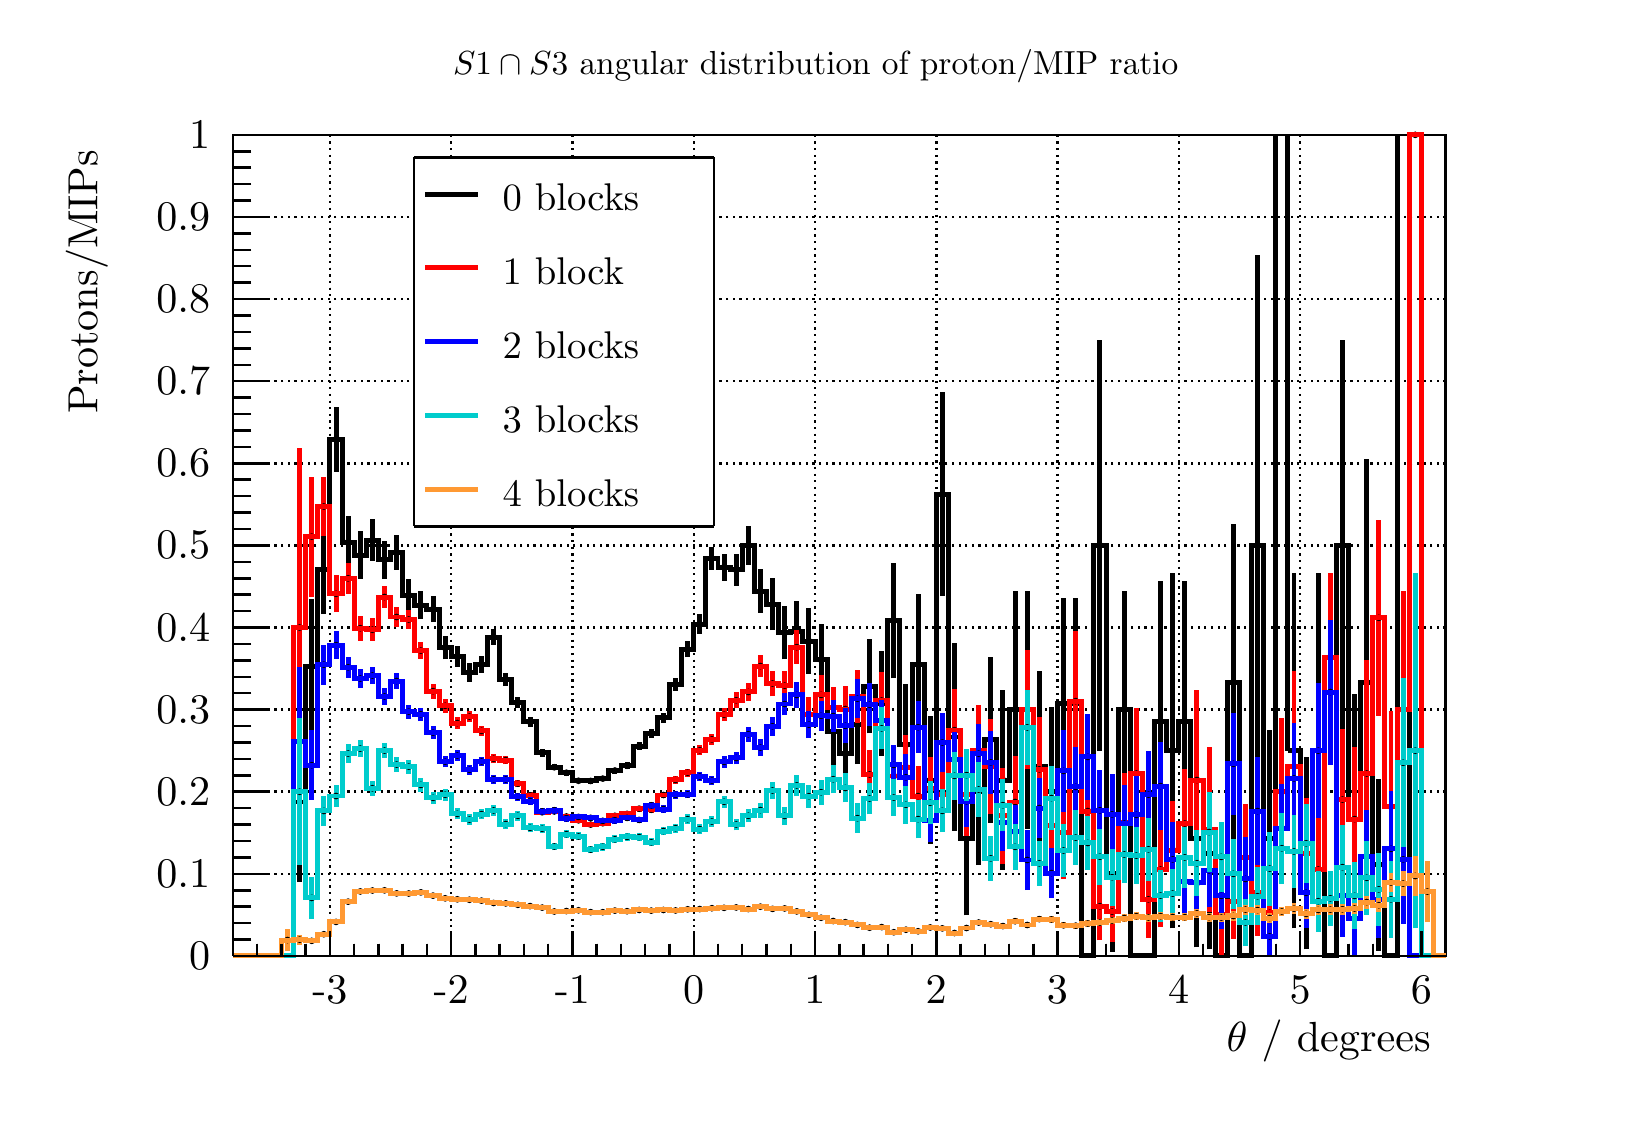
\begin{tikzpicture}
\pgfdeclareplotmark{cross} {
\pgfpathmoveto{\pgfpoint{-0.3\pgfplotmarksize}{\pgfplotmarksize}}
\pgfpathlineto{\pgfpoint{+0.3\pgfplotmarksize}{\pgfplotmarksize}}
\pgfpathlineto{\pgfpoint{+0.3\pgfplotmarksize}{0.3\pgfplotmarksize}}
\pgfpathlineto{\pgfpoint{+1\pgfplotmarksize}{0.3\pgfplotmarksize}}
\pgfpathlineto{\pgfpoint{+1\pgfplotmarksize}{-0.3\pgfplotmarksize}}
\pgfpathlineto{\pgfpoint{+0.3\pgfplotmarksize}{-0.3\pgfplotmarksize}}
\pgfpathlineto{\pgfpoint{+0.3\pgfplotmarksize}{-1.\pgfplotmarksize}}
\pgfpathlineto{\pgfpoint{-0.3\pgfplotmarksize}{-1.\pgfplotmarksize}}
\pgfpathlineto{\pgfpoint{-0.3\pgfplotmarksize}{-0.3\pgfplotmarksize}}
\pgfpathlineto{\pgfpoint{-1.\pgfplotmarksize}{-0.3\pgfplotmarksize}}
\pgfpathlineto{\pgfpoint{-1.\pgfplotmarksize}{0.3\pgfplotmarksize}}
\pgfpathlineto{\pgfpoint{-0.3\pgfplotmarksize}{0.3\pgfplotmarksize}}
\pgfpathclose
\pgfusepathqstroke
}
\pgfdeclareplotmark{cross*} {
\pgfpathmoveto{\pgfpoint{-0.3\pgfplotmarksize}{\pgfplotmarksize}}
\pgfpathlineto{\pgfpoint{+0.3\pgfplotmarksize}{\pgfplotmarksize}}
\pgfpathlineto{\pgfpoint{+0.3\pgfplotmarksize}{0.3\pgfplotmarksize}}
\pgfpathlineto{\pgfpoint{+1\pgfplotmarksize}{0.3\pgfplotmarksize}}
\pgfpathlineto{\pgfpoint{+1\pgfplotmarksize}{-0.3\pgfplotmarksize}}
\pgfpathlineto{\pgfpoint{+0.3\pgfplotmarksize}{-0.3\pgfplotmarksize}}
\pgfpathlineto{\pgfpoint{+0.3\pgfplotmarksize}{-1.\pgfplotmarksize}}
\pgfpathlineto{\pgfpoint{-0.3\pgfplotmarksize}{-1.\pgfplotmarksize}}
\pgfpathlineto{\pgfpoint{-0.3\pgfplotmarksize}{-0.3\pgfplotmarksize}}
\pgfpathlineto{\pgfpoint{-1.\pgfplotmarksize}{-0.3\pgfplotmarksize}}
\pgfpathlineto{\pgfpoint{-1.\pgfplotmarksize}{0.3\pgfplotmarksize}}
\pgfpathlineto{\pgfpoint{-0.3\pgfplotmarksize}{0.3\pgfplotmarksize}}
\pgfpathclose
\pgfusepathqfillstroke
}
\pgfdeclareplotmark{newstar} {
\pgfpathmoveto{\pgfqpoint{0pt}{\pgfplotmarksize}}
\pgfpathlineto{\pgfqpointpolar{44}{0.5\pgfplotmarksize}}
\pgfpathlineto{\pgfqpointpolar{18}{\pgfplotmarksize}}
\pgfpathlineto{\pgfqpointpolar{-20}{0.5\pgfplotmarksize}}
\pgfpathlineto{\pgfqpointpolar{-54}{\pgfplotmarksize}}
\pgfpathlineto{\pgfqpointpolar{-90}{0.5\pgfplotmarksize}}
\pgfpathlineto{\pgfqpointpolar{234}{\pgfplotmarksize}}
\pgfpathlineto{\pgfqpointpolar{198}{0.5\pgfplotmarksize}}
\pgfpathlineto{\pgfqpointpolar{162}{\pgfplotmarksize}}
\pgfpathlineto{\pgfqpointpolar{134}{0.5\pgfplotmarksize}}
\pgfpathclose
\pgfusepathqstroke
}
\pgfdeclareplotmark{newstar*} {
\pgfpathmoveto{\pgfqpoint{0pt}{\pgfplotmarksize}}
\pgfpathlineto{\pgfqpointpolar{44}{0.5\pgfplotmarksize}}
\pgfpathlineto{\pgfqpointpolar{18}{\pgfplotmarksize}}
\pgfpathlineto{\pgfqpointpolar{-20}{0.5\pgfplotmarksize}}
\pgfpathlineto{\pgfqpointpolar{-54}{\pgfplotmarksize}}
\pgfpathlineto{\pgfqpointpolar{-90}{0.5\pgfplotmarksize}}
\pgfpathlineto{\pgfqpointpolar{234}{\pgfplotmarksize}}
\pgfpathlineto{\pgfqpointpolar{198}{0.5\pgfplotmarksize}}
\pgfpathlineto{\pgfqpointpolar{162}{\pgfplotmarksize}}
\pgfpathlineto{\pgfqpointpolar{134}{0.5\pgfplotmarksize}}
\pgfpathclose
\pgfusepathqfillstroke
}
\definecolor{c}{rgb}{1,1,1};
\draw [color=c, fill=c] (0,0) rectangle (20,13.5429);
\draw [color=c, fill=c] (2.6,1.76057) rectangle (18,12.1886);
\definecolor{c}{rgb}{0,0,0};
\draw [c,line width=0.9] (2.6,1.76057) -- (2.6,12.1886) -- (18,12.1886) -- (18,1.76057) -- (2.6,1.76057);
\definecolor{c}{rgb}{1,1,1};
\draw [color=c, fill=c] (2.6,1.76057) rectangle (18,12.1886);
\definecolor{c}{rgb}{0,0,0};
\draw [c,line width=0.9] (2.6,1.76057) -- (2.6,12.1886) -- (18,12.1886) -- (18,1.76057) -- (2.6,1.76057);
\draw [c,line width=0.9] (2.6,1.76057) -- (18,1.76057);
\draw [c,dash pattern=on 0.80pt off 1.60pt ,line width=0.9] (3.832,12.1886) -- (3.832,1.76057);
\draw [c,dash pattern=on 0.80pt off 1.60pt ,line width=0.9] (5.372,12.1886) -- (5.372,1.76057);
\draw [c,dash pattern=on 0.80pt off 1.60pt ,line width=0.9] (6.912,12.1886) -- (6.912,1.76057);
\draw [c,dash pattern=on 0.80pt off 1.60pt ,line width=0.9] (8.452,12.1886) -- (8.452,1.76057);
\draw [c,dash pattern=on 0.80pt off 1.60pt ,line width=0.9] (9.992,12.1886) -- (9.992,1.76057);
\draw [c,dash pattern=on 0.80pt off 1.60pt ,line width=0.9] (11.532,12.1886) -- (11.532,1.76057);
\draw [c,dash pattern=on 0.80pt off 1.60pt ,line width=0.9] (13.072,12.1886) -- (13.072,1.76057);
\draw [c,dash pattern=on 0.80pt off 1.60pt ,line width=0.9] (14.612,12.1886) -- (14.612,1.76057);
\draw [c,dash pattern=on 0.80pt off 1.60pt ,line width=0.9] (16.152,12.1886) -- (16.152,1.76057);
\draw [c,dash pattern=on 0.80pt off 1.60pt ,line width=0.9] (17.692,12.1886) -- (17.692,1.76057);
\draw [c,dash pattern=on 0.80pt off 1.60pt ,line width=0.9] (3.832,12.1886) -- (3.832,1.76057);
\draw [c,dash pattern=on 0.80pt off 1.60pt ,line width=0.9] (17.692,12.1886) -- (17.692,1.76057);
\draw [c,line width=0.9] (2.6,1.76057) -- (2.6,12.1886);
\draw [c,dash pattern=on 0.80pt off 1.60pt ,line width=0.9] (18,1.76057) -- (2.6,1.76057);
\draw [c,dash pattern=on 0.80pt off 1.60pt ,line width=0.9] (18,2.80337) -- (2.6,2.80337);
\draw [c,dash pattern=on 0.80pt off 1.60pt ,line width=0.9] (18,3.84617) -- (2.6,3.84617);
\draw [c,dash pattern=on 0.80pt off 1.60pt ,line width=0.9] (18,4.88897) -- (2.6,4.88897);
\draw [c,dash pattern=on 0.80pt off 1.60pt ,line width=0.9] (18,5.93177) -- (2.6,5.93177);
\draw [c,dash pattern=on 0.80pt off 1.60pt ,line width=0.9] (18,6.97457) -- (2.6,6.97457);
\draw [c,dash pattern=on 0.80pt off 1.60pt ,line width=0.9] (18,8.01737) -- (2.6,8.01737);
\draw [c,dash pattern=on 0.80pt off 1.60pt ,line width=0.9] (18,9.06017) -- (2.6,9.06017);
\draw [c,dash pattern=on 0.80pt off 1.60pt ,line width=0.9] (18,10.103) -- (2.6,10.103);
\draw [c,dash pattern=on 0.80pt off 1.60pt ,line width=0.9] (18,11.1458) -- (2.6,11.1458);
\draw [c,dash pattern=on 0.80pt off 1.60pt ,line width=0.9] (18,12.1886) -- (2.6,12.1886);
\definecolor{c}{rgb}{0,0,0.6};
\draw [c,line width=0.9] (2.6,1.76057) -- (2.754,1.76057) -- (2.754,1.76057) -- (2.908,1.76057) -- (2.908,1.76057) -- (3.062,1.76057) -- (3.062,1.76057) -- (3.216,1.76057) -- (3.216,1.76057) -- (3.37,1.76057) -- (3.37,1.76057) -- (3.524,1.76057) --
 (3.524,1.76057) -- (3.678,1.76057) -- (3.678,1.76057) -- (3.832,1.76057) -- (3.832,1.76057) -- (3.986,1.76057) -- (3.986,1.76057) -- (4.14,1.76057) -- (4.14,1.76057) -- (4.294,1.76057) -- (4.294,1.76057) -- (4.448,1.76057) -- (4.448,1.76057) --
 (4.602,1.76057) -- (4.602,1.76057) -- (4.756,1.76057) -- (4.756,1.76057) -- (4.91,1.76057) -- (4.91,1.76057) -- (5.064,1.76057) -- (5.064,1.76057) -- (5.218,1.76057) -- (5.218,1.76057) -- (5.372,1.76057) -- (5.372,1.76057) -- (5.526,1.76057) --
 (5.526,1.76057) -- (5.68,1.76057) -- (5.68,1.76057) -- (5.834,1.76057) -- (5.834,1.76057) -- (5.988,1.76057) -- (5.988,1.76057) -- (6.142,1.76057) -- (6.142,1.76057) -- (6.296,1.76057) -- (6.296,1.76057) -- (6.45,1.76057) -- (6.45,1.76057) --
 (6.604,1.76057) -- (6.604,1.76057) -- (6.758,1.76057) -- (6.758,1.76057) -- (6.912,1.76057) -- (6.912,1.76057) -- (7.066,1.76057) -- (7.066,1.76057) -- (7.22,1.76057) -- (7.22,1.76057) -- (7.374,1.76057) -- (7.374,1.76057) -- (7.528,1.76057) --
 (7.528,1.76057) -- (7.682,1.76057) -- (7.682,1.76057) -- (7.836,1.76057) -- (7.836,1.76057) -- (7.99,1.76057) -- (7.99,1.76057) -- (8.144,1.76057) -- (8.144,1.76057) -- (8.298,1.76057) -- (8.298,1.76057) -- (8.452,1.76057) -- (8.452,1.76057) --
 (8.606,1.76057) -- (8.606,1.76057) -- (8.76,1.76057) -- (8.76,1.76057) -- (8.914,1.76057) -- (8.914,1.76057) -- (9.068,1.76057) -- (9.068,1.76057) -- (9.222,1.76057) -- (9.222,1.76057) -- (9.376,1.76057) -- (9.376,1.76057) -- (9.53,1.76057) --
 (9.53,1.76057) -- (9.684,1.76057) -- (9.684,1.76057) -- (9.838,1.76057) -- (9.838,1.76057) -- (9.992,1.76057) -- (9.992,1.76057) -- (10.146,1.76057) -- (10.146,1.76057) -- (10.3,1.76057) -- (10.3,1.76057) -- (10.454,1.76057) -- (10.454,1.76057) --
 (10.608,1.76057) -- (10.608,1.76057) -- (10.762,1.76057) -- (10.762,1.76057) -- (10.916,1.76057) -- (10.916,1.76057) -- (11.07,1.76057) -- (11.07,1.76057) -- (11.224,1.76057) -- (11.224,1.76057) -- (11.378,1.76057) -- (11.378,1.76057) --
 (11.532,1.76057) -- (11.532,1.76057) -- (11.686,1.76057) -- (11.686,1.76057) -- (11.84,1.76057) -- (11.84,1.76057) -- (11.994,1.76057) -- (11.994,1.76057) -- (12.148,1.76057) -- (12.148,1.76057) -- (12.302,1.76057) -- (12.302,1.76057) --
 (12.456,1.76057) -- (12.456,1.76057) -- (12.61,1.76057) -- (12.61,1.76057) -- (12.764,1.76057) -- (12.764,1.76057) -- (12.918,1.76057) -- (12.918,1.76057) -- (13.072,1.76057) -- (13.072,1.76057) -- (13.226,1.76057) -- (13.226,1.76057) --
 (13.38,1.76057) -- (13.38,1.76057) -- (13.534,1.76057) -- (13.534,1.76057) -- (13.688,1.76057) -- (13.688,1.76057) -- (13.842,1.76057) -- (13.842,1.76057) -- (13.996,1.76057) -- (13.996,1.76057) -- (14.15,1.76057) -- (14.15,1.76057) --
 (14.304,1.76057) -- (14.304,1.76057) -- (14.458,1.76057) -- (14.458,1.76057) -- (14.612,1.76057) -- (14.612,1.76057) -- (14.766,1.76057) -- (14.766,1.76057) -- (14.92,1.76057) -- (14.92,1.76057) -- (15.074,1.76057) -- (15.074,1.76057) --
 (15.228,1.76057) -- (15.228,1.76057) -- (15.382,1.76057) -- (15.382,1.76057) -- (15.536,1.76057) -- (15.536,1.76057) -- (15.69,1.76057) -- (15.69,1.76057) -- (15.844,1.76057) -- (15.844,1.76057) -- (15.998,1.76057) -- (15.998,1.76057) --
 (16.152,1.76057) -- (16.152,1.76057) -- (16.306,1.76057) -- (16.306,1.76057) -- (16.46,1.76057) -- (16.46,1.76057) -- (16.614,1.76057) -- (16.614,1.76057) -- (16.768,1.76057) -- (16.768,1.76057) -- (16.922,1.76057) -- (16.922,1.76057) --
 (17.076,1.76057) -- (17.076,1.76057) -- (17.23,1.76057) -- (17.23,1.76057) -- (17.384,1.76057) -- (17.384,1.76057) -- (17.538,1.76057) -- (17.538,1.76057) -- (17.692,1.76057) -- (17.692,1.76057) -- (17.846,1.76057) -- (17.846,1.76057) --
 (18,1.76057);
\definecolor{c}{rgb}{0,0,0};
\draw [c,line width=0.9] (2.6,1.76057) -- (18,1.76057);
\draw [c,line width=0.9] (3.832,2.07341) -- (3.832,1.76057);
\draw [c,line width=0.9] (4.14,1.91699) -- (4.14,1.76057);
\draw [c,line width=0.9] (4.448,1.91699) -- (4.448,1.76057);
\draw [c,line width=0.9] (4.756,1.91699) -- (4.756,1.76057);
\draw [c,line width=0.9] (5.064,1.91699) -- (5.064,1.76057);
\draw [c,line width=0.9] (5.372,2.07341) -- (5.372,1.76057);
\draw [c,line width=0.9] (5.68,1.91699) -- (5.68,1.76057);
\draw [c,line width=0.9] (5.988,1.91699) -- (5.988,1.76057);
\draw [c,line width=0.9] (6.296,1.91699) -- (6.296,1.76057);
\draw [c,line width=0.9] (6.604,1.91699) -- (6.604,1.76057);
\draw [c,line width=0.9] (6.912,2.07341) -- (6.912,1.76057);
\draw [c,line width=0.9] (7.22,1.91699) -- (7.22,1.76057);
\draw [c,line width=0.9] (7.528,1.91699) -- (7.528,1.76057);
\draw [c,line width=0.9] (7.836,1.91699) -- (7.836,1.76057);
\draw [c,line width=0.9] (8.144,1.91699) -- (8.144,1.76057);
\draw [c,line width=0.9] (8.452,2.07341) -- (8.452,1.76057);
\draw [c,line width=0.9] (8.76,1.91699) -- (8.76,1.76057);
\draw [c,line width=0.9] (9.068,1.91699) -- (9.068,1.76057);
\draw [c,line width=0.9] (9.376,1.91699) -- (9.376,1.76057);
\draw [c,line width=0.9] (9.684,1.91699) -- (9.684,1.76057);
\draw [c,line width=0.9] (9.992,2.07341) -- (9.992,1.76057);
\draw [c,line width=0.9] (10.3,1.91699) -- (10.3,1.76057);
\draw [c,line width=0.9] (10.608,1.91699) -- (10.608,1.76057);
\draw [c,line width=0.9] (10.916,1.91699) -- (10.916,1.76057);
\draw [c,line width=0.9] (11.224,1.91699) -- (11.224,1.76057);
\draw [c,line width=0.9] (11.532,2.07341) -- (11.532,1.76057);
\draw [c,line width=0.9] (11.84,1.91699) -- (11.84,1.76057);
\draw [c,line width=0.9] (12.148,1.91699) -- (12.148,1.76057);
\draw [c,line width=0.9] (12.456,1.91699) -- (12.456,1.76057);
\draw [c,line width=0.9] (12.764,1.91699) -- (12.764,1.76057);
\draw [c,line width=0.9] (13.072,2.07341) -- (13.072,1.76057);
\draw [c,line width=0.9] (13.38,1.91699) -- (13.38,1.76057);
\draw [c,line width=0.9] (13.688,1.91699) -- (13.688,1.76057);
\draw [c,line width=0.9] (13.996,1.91699) -- (13.996,1.76057);
\draw [c,line width=0.9] (14.304,1.91699) -- (14.304,1.76057);
\draw [c,line width=0.9] (14.612,2.07341) -- (14.612,1.76057);
\draw [c,line width=0.9] (14.92,1.91699) -- (14.92,1.76057);
\draw [c,line width=0.9] (15.228,1.91699) -- (15.228,1.76057);
\draw [c,line width=0.9] (15.536,1.91699) -- (15.536,1.76057);
\draw [c,line width=0.9] (15.844,1.91699) -- (15.844,1.76057);
\draw [c,line width=0.9] (16.152,2.07341) -- (16.152,1.76057);
\draw [c,line width=0.9] (16.46,1.91699) -- (16.46,1.76057);
\draw [c,line width=0.9] (16.768,1.91699) -- (16.768,1.76057);
\draw [c,line width=0.9] (17.076,1.91699) -- (17.076,1.76057);
\draw [c,line width=0.9] (17.384,1.91699) -- (17.384,1.76057);
\draw [c,line width=0.9] (17.692,2.07341) -- (17.692,1.76057);
\draw [c,line width=0.9] (3.832,2.07341) -- (3.832,1.76057);
\draw [c,line width=0.9] (3.524,1.91699) -- (3.524,1.76057);
\draw [c,line width=0.9] (3.216,1.91699) -- (3.216,1.76057);
\draw [c,line width=0.9] (2.908,1.91699) -- (2.908,1.76057);
\draw [c,line width=0.9] (17.692,2.07341) -- (17.692,1.76057);
\draw [anchor=base] (3.832,1.15114) node[scale=1.52295, color=c, rotate=0]{-3};
\draw [anchor=base] (5.372,1.15114) node[scale=1.52295, color=c, rotate=0]{-2};
\draw [anchor=base] (6.912,1.15114) node[scale=1.52295, color=c, rotate=0]{-1};
\draw [anchor=base] (8.452,1.15114) node[scale=1.52295, color=c, rotate=0]{0};
\draw [anchor=base] (9.992,1.15114) node[scale=1.52295, color=c, rotate=0]{1};
\draw [anchor=base] (11.532,1.15114) node[scale=1.52295, color=c, rotate=0]{2};
\draw [anchor=base] (13.072,1.15114) node[scale=1.52295, color=c, rotate=0]{3};
\draw [anchor=base] (14.612,1.15114) node[scale=1.52295, color=c, rotate=0]{4};
\draw [anchor=base] (16.152,1.15114) node[scale=1.52295, color=c, rotate=0]{5};
\draw [anchor=base] (17.692,1.15114) node[scale=1.52295, color=c, rotate=0]{6};
\draw [anchor= east] (18,0.677143) node[scale=1.52295, color=c, rotate=0]{$ \theta$ / degrees};
\draw [c,line width=0.9] (2.6,1.76057) -- (2.6,12.1886);
\draw [c,line width=0.9] (3.062,1.76057) -- (2.6,1.76057);
\draw [c,line width=0.9] (2.831,1.96913) -- (2.6,1.96913);
\draw [c,line width=0.9] (2.831,2.17769) -- (2.6,2.17769);
\draw [c,line width=0.9] (2.831,2.38625) -- (2.6,2.38625);
\draw [c,line width=0.9] (2.831,2.59481) -- (2.6,2.59481);
\draw [c,line width=0.9] (3.062,2.80337) -- (2.6,2.80337);
\draw [c,line width=0.9] (2.831,3.01193) -- (2.6,3.01193);
\draw [c,line width=0.9] (2.831,3.22049) -- (2.6,3.22049);
\draw [c,line width=0.9] (2.831,3.42905) -- (2.6,3.42905);
\draw [c,line width=0.9] (2.831,3.63761) -- (2.6,3.63761);
\draw [c,line width=0.9] (3.062,3.84617) -- (2.6,3.84617);
\draw [c,line width=0.9] (2.831,4.05473) -- (2.6,4.05473);
\draw [c,line width=0.9] (2.831,4.26329) -- (2.6,4.26329);
\draw [c,line width=0.9] (2.831,4.47185) -- (2.6,4.47185);
\draw [c,line width=0.9] (2.831,4.68041) -- (2.6,4.68041);
\draw [c,line width=0.9] (3.062,4.88897) -- (2.6,4.88897);
\draw [c,line width=0.9] (2.831,5.09753) -- (2.6,5.09753);
\draw [c,line width=0.9] (2.831,5.30609) -- (2.6,5.30609);
\draw [c,line width=0.9] (2.831,5.51465) -- (2.6,5.51465);
\draw [c,line width=0.9] (2.831,5.72321) -- (2.6,5.72321);
\draw [c,line width=0.9] (3.062,5.93177) -- (2.6,5.93177);
\draw [c,line width=0.9] (2.831,6.14033) -- (2.6,6.14033);
\draw [c,line width=0.9] (2.831,6.34889) -- (2.6,6.34889);
\draw [c,line width=0.9] (2.831,6.55745) -- (2.6,6.55745);
\draw [c,line width=0.9] (2.831,6.76601) -- (2.6,6.76601);
\draw [c,line width=0.9] (3.062,6.97457) -- (2.6,6.97457);
\draw [c,line width=0.9] (2.831,7.18313) -- (2.6,7.18313);
\draw [c,line width=0.9] (2.831,7.39169) -- (2.6,7.39169);
\draw [c,line width=0.9] (2.831,7.60025) -- (2.6,7.60025);
\draw [c,line width=0.9] (2.831,7.80881) -- (2.6,7.80881);
\draw [c,line width=0.9] (3.062,8.01737) -- (2.6,8.01737);
\draw [c,line width=0.9] (2.831,8.22593) -- (2.6,8.22593);
\draw [c,line width=0.9] (2.831,8.43449) -- (2.6,8.43449);
\draw [c,line width=0.9] (2.831,8.64305) -- (2.6,8.64305);
\draw [c,line width=0.9] (2.831,8.85161) -- (2.6,8.85161);
\draw [c,line width=0.9] (3.062,9.06017) -- (2.6,9.06017);
\draw [c,line width=0.9] (2.831,9.26873) -- (2.6,9.26873);
\draw [c,line width=0.9] (2.831,9.47729) -- (2.6,9.47729);
\draw [c,line width=0.9] (2.831,9.68585) -- (2.6,9.68585);
\draw [c,line width=0.9] (2.831,9.89441) -- (2.6,9.89441);
\draw [c,line width=0.9] (3.062,10.103) -- (2.6,10.103);
\draw [c,line width=0.9] (2.831,10.3115) -- (2.6,10.3115);
\draw [c,line width=0.9] (2.831,10.5201) -- (2.6,10.5201);
\draw [c,line width=0.9] (2.831,10.7287) -- (2.6,10.7287);
\draw [c,line width=0.9] (2.831,10.9372) -- (2.6,10.9372);
\draw [c,line width=0.9] (3.062,11.1458) -- (2.6,11.1458);
\draw [c,line width=0.9] (2.831,11.3543) -- (2.6,11.3543);
\draw [c,line width=0.9] (2.831,11.5629) -- (2.6,11.5629);
\draw [c,line width=0.9] (2.831,11.7715) -- (2.6,11.7715);
\draw [c,line width=0.9] (2.831,11.98) -- (2.6,11.98);
\draw [c,line width=0.9] (3.062,12.1886) -- (2.6,12.1886);
\draw [anchor= east] (2.5,1.76057) node[scale=1.52295, color=c, rotate=0]{0};
\draw [anchor= east] (2.5,2.80337) node[scale=1.52295, color=c, rotate=0]{0.1};
\draw [anchor= east] (2.5,3.84617) node[scale=1.52295, color=c, rotate=0]{0.2};
\draw [anchor= east] (2.5,4.88897) node[scale=1.52295, color=c, rotate=0]{0.3};
\draw [anchor= east] (2.5,5.93177) node[scale=1.52295, color=c, rotate=0]{0.4};
\draw [anchor= east] (2.5,6.97457) node[scale=1.52295, color=c, rotate=0]{0.5};
\draw [anchor= east] (2.5,8.01737) node[scale=1.52295, color=c, rotate=0]{0.6};
\draw [anchor= east] (2.5,9.06017) node[scale=1.52295, color=c, rotate=0]{0.7};
\draw [anchor= east] (2.5,10.103) node[scale=1.52295, color=c, rotate=0]{0.8};
\draw [anchor= east] (2.5,11.1458) node[scale=1.52295, color=c, rotate=0]{0.9};
\draw [anchor= east] (2.5,12.1886) node[scale=1.52295, color=c, rotate=0]{1};
\draw [anchor= east] (0.742857,12.1886) node[scale=1.52295, color=c, rotate=90]{  Protons/MIPs};
\draw [c,line width=1.8] (3.447,2.69828) -- (3.447,3.71582);
\draw [c,line width=1.8] (3.447,3.71582) -- (3.447,4.73337);
\foreach \P in {(3.447,3.71582)}{\draw[mark options={color=c,fill=c},mark size=2.402402pt,mark=*,mark size=1pt] plot coordinates {\P};}
\draw [c,line width=1.8] (3.601,4.5864) -- (3.601,5.44104);
\draw [c,line width=1.8] (3.601,5.44104) -- (3.601,6.29568);
\foreach \P in {(3.601,5.44104)}{\draw[mark options={color=c,fill=c},mark size=2.402402pt,mark=*,mark size=1pt] plot coordinates {\P};}
\draw [c,line width=1.8] (3.755,6.10331) -- (3.755,6.66787);
\draw [c,line width=1.8] (3.755,6.66787) -- (3.755,7.23242);
\foreach \P in {(3.755,6.66787)}{\draw[mark options={color=c,fill=c},mark size=2.402402pt,mark=*,mark size=1pt] plot coordinates {\P};}
\draw [c,line width=1.8] (3.909,7.91132) -- (3.909,8.32123);
\draw [c,line width=1.8] (3.909,8.32123) -- (3.909,8.73115);
\foreach \P in {(3.909,8.32123)}{\draw[mark options={color=c,fill=c},mark size=2.402402pt,mark=*,mark size=1pt] plot coordinates {\P};}
\draw [c,line width=1.8] (4.063,6.68653) -- (4.063,7.01628);
\draw [c,line width=1.8] (4.063,7.01628) -- (4.063,7.34604);
\foreach \P in {(4.063,7.01628)}{\draw[mark options={color=c,fill=c},mark size=2.402402pt,mark=*,mark size=1pt] plot coordinates {\P};}
\draw [c,line width=1.8] (4.217,6.54736) -- (4.217,6.85085);
\draw [c,line width=1.8] (4.217,6.85085) -- (4.217,7.15433);
\foreach \P in {(4.217,6.85085)}{\draw[mark options={color=c,fill=c},mark size=2.402402pt,mark=*,mark size=1pt] plot coordinates {\P};}
\draw [c,line width=1.8] (4.371,6.77692) -- (4.371,7.04194);
\draw [c,line width=1.8] (4.371,7.04194) -- (4.371,7.30696);
\foreach \P in {(4.371,7.04194)}{\draw[mark options={color=c,fill=c},mark size=2.402402pt,mark=*,mark size=1pt] plot coordinates {\P};}
\draw [c,line width=1.8] (4.525,6.54627) -- (4.525,6.79082);
\draw [c,line width=1.8] (4.525,6.79082) -- (4.525,7.03537);
\foreach \P in {(4.525,6.79082)}{\draw[mark options={color=c,fill=c},mark size=2.402402pt,mark=*,mark size=1pt] plot coordinates {\P};}
\draw [c,line width=1.8] (4.679,6.66261) -- (4.679,6.88212);
\draw [c,line width=1.8] (4.679,6.88212) -- (4.679,7.10164);
\foreach \P in {(4.679,6.88212)}{\draw[mark options={color=c,fill=c},mark size=2.402402pt,mark=*,mark size=1pt] plot coordinates {\P};}
\draw [c,line width=1.8] (4.833,6.14124) -- (4.833,6.34378);
\draw [c,line width=1.8] (4.833,6.34378) -- (4.833,6.54632);
\foreach \P in {(4.833,6.34378)}{\draw[mark options={color=c,fill=c},mark size=2.402402pt,mark=*,mark size=1pt] plot coordinates {\P};}
\draw [c,line width=1.8] (4.987,6.03439) -- (4.987,6.21354);
\draw [c,line width=1.8] (4.987,6.21354) -- (4.987,6.39269);
\foreach \P in {(4.987,6.21354)}{\draw[mark options={color=c,fill=c},mark size=2.402402pt,mark=*,mark size=1pt] plot coordinates {\P};}
\draw [c,line width=1.8] (5.141,6.00133) -- (5.141,6.16587);
\draw [c,line width=1.8] (5.141,6.16587) -- (5.141,6.33041);
\foreach \P in {(5.141,6.16587)}{\draw[mark options={color=c,fill=c},mark size=2.402402pt,mark=*,mark size=1pt] plot coordinates {\P};}
\draw [c,line width=1.8] (5.295,5.52618) -- (5.295,5.67328);
\draw [c,line width=1.8] (5.295,5.67328) -- (5.295,5.82039);
\foreach \P in {(5.295,5.67328)}{\draw[mark options={color=c,fill=c},mark size=2.402402pt,mark=*,mark size=1pt] plot coordinates {\P};}
\draw [c,line width=1.8] (5.449,5.43471) -- (5.449,5.5688);
\draw [c,line width=1.8] (5.449,5.5688) -- (5.449,5.70289);
\foreach \P in {(5.449,5.5688)}{\draw[mark options={color=c,fill=c},mark size=2.402402pt,mark=*,mark size=1pt] plot coordinates {\P};}
\draw [c,line width=1.8] (5.603,5.24489) -- (5.603,5.36319);
\draw [c,line width=1.8] (5.603,5.36319) -- (5.603,5.48149);
\foreach \P in {(5.603,5.36319)}{\draw[mark options={color=c,fill=c},mark size=2.402402pt,mark=*,mark size=1pt] plot coordinates {\P};}
\draw [c,line width=1.8] (5.757,5.35586) -- (5.757,5.46365);
\draw [c,line width=1.8] (5.757,5.46365) -- (5.757,5.57145);
\foreach \P in {(5.757,5.46365)}{\draw[mark options={color=c,fill=c},mark size=2.402402pt,mark=*,mark size=1pt] plot coordinates {\P};}
\draw [c,line width=1.8] (5.911,5.71068) -- (5.911,5.80974);
\draw [c,line width=1.8] (5.911,5.80974) -- (5.911,5.9088);
\foreach \P in {(5.911,5.80974)}{\draw[mark options={color=c,fill=c},mark size=2.402402pt,mark=*,mark size=1pt] plot coordinates {\P};}
\draw [c,line width=1.8] (6.065,5.18882) -- (6.065,5.27358);
\draw [c,line width=1.8] (6.065,5.27358) -- (6.065,5.35835);
\foreach \P in {(6.065,5.27358)}{\draw[mark options={color=c,fill=c},mark size=2.402402pt,mark=*,mark size=1pt] plot coordinates {\P};}
\draw [c,line width=1.8] (6.219,4.90855) -- (6.219,4.97895);
\draw [c,line width=1.8] (6.219,4.97895) -- (6.219,5.04935);
\foreach \P in {(6.219,4.97895)}{\draw[mark options={color=c,fill=c},mark size=2.402402pt,mark=*,mark size=1pt] plot coordinates {\P};}
\draw [c,line width=1.8] (6.373,4.67359) -- (6.373,4.73253);
\draw [c,line width=1.8] (6.373,4.73253) -- (6.373,4.79147);
\foreach \P in {(6.373,4.73253)}{\draw[mark options={color=c,fill=c},mark size=2.402402pt,mark=*,mark size=1pt] plot coordinates {\P};}
\draw [c,line width=1.8] (6.527,4.29323) -- (6.527,4.34135);
\draw [c,line width=1.8] (6.527,4.34135) -- (6.527,4.38946);
\foreach \P in {(6.527,4.34135)}{\draw[mark options={color=c,fill=c},mark size=2.402402pt,mark=*,mark size=1pt] plot coordinates {\P};}
\draw [c,line width=1.8] (6.681,4.11642) -- (6.681,4.1571);
\draw [c,line width=1.8] (6.681,4.1571) -- (6.681,4.19778);
\foreach \P in {(6.681,4.1571)}{\draw[mark options={color=c,fill=c},mark size=2.402402pt,mark=*,mark size=1pt] plot coordinates {\P};}
\draw [c,line width=1.8] (6.835,4.05142) -- (6.835,4.08804);
\draw [c,line width=1.8] (6.835,4.08804) -- (6.835,4.12465);
\foreach \P in {(6.835,4.08804)}{\draw[mark options={color=c,fill=c},mark size=2.402402pt,mark=*,mark size=1pt] plot coordinates {\P};}
\draw [c,line width=1.8] (6.989,3.95156) -- (6.989,3.98547);
\draw [c,line width=1.8] (6.989,3.98547) -- (6.989,4.01939);
\foreach \P in {(6.989,3.98547)}{\draw[mark options={color=c,fill=c},mark size=2.402402pt,mark=*,mark size=1pt] plot coordinates {\P};}
\draw [c,line width=1.8] (7.143,3.94992) -- (7.143,3.98352);
\draw [c,line width=1.8] (7.143,3.98352) -- (7.143,4.01712);
\foreach \P in {(7.143,3.98352)}{\draw[mark options={color=c,fill=c},mark size=2.402402pt,mark=*,mark size=1pt] plot coordinates {\P};}
\draw [c,line width=1.8] (7.297,3.97822) -- (7.297,4.013);
\draw [c,line width=1.8] (7.297,4.013) -- (7.297,4.04777);
\foreach \P in {(7.297,4.013)}{\draw[mark options={color=c,fill=c},mark size=2.402402pt,mark=*,mark size=1pt] plot coordinates {\P};}
\draw [c,line width=1.8] (7.451,4.07786) -- (7.451,4.11597);
\draw [c,line width=1.8] (7.451,4.11597) -- (7.451,4.15409);
\foreach \P in {(7.451,4.11597)}{\draw[mark options={color=c,fill=c},mark size=2.402402pt,mark=*,mark size=1pt] plot coordinates {\P};}
\draw [c,line width=1.8] (7.605,4.13387) -- (7.605,4.17615);
\draw [c,line width=1.8] (7.605,4.17615) -- (7.605,4.21843);
\foreach \P in {(7.605,4.17615)}{\draw[mark options={color=c,fill=c},mark size=2.402402pt,mark=*,mark size=1pt] plot coordinates {\P};}
\draw [c,line width=1.8] (7.759,4.37721) -- (7.759,4.42618);
\draw [c,line width=1.8] (7.759,4.42618) -- (7.759,4.47514);
\foreach \P in {(7.759,4.42618)}{\draw[mark options={color=c,fill=c},mark size=2.402402pt,mark=*,mark size=1pt] plot coordinates {\P};}
\draw [c,line width=1.8] (7.913,4.52827) -- (7.913,4.58456);
\draw [c,line width=1.8] (7.913,4.58456) -- (7.913,4.64086);
\foreach \P in {(7.913,4.58456)}{\draw[mark options={color=c,fill=c},mark size=2.402402pt,mark=*,mark size=1pt] plot coordinates {\P};}
\draw [c,line width=1.8] (8.067,4.71813) -- (8.067,4.78436);
\draw [c,line width=1.8] (8.067,4.78436) -- (8.067,4.8506);
\foreach \P in {(8.067,4.78436)}{\draw[mark options={color=c,fill=c},mark size=2.402402pt,mark=*,mark size=1pt] plot coordinates {\P};}
\draw [c,line width=1.8] (8.221,5.13176) -- (8.221,5.21346);
\draw [c,line width=1.8] (8.221,5.21346) -- (8.221,5.29515);
\foreach \P in {(8.221,5.21346)}{\draw[mark options={color=c,fill=c},mark size=2.402402pt,mark=*,mark size=1pt] plot coordinates {\P};}
\draw [c,line width=1.8] (8.375,5.55691) -- (8.375,5.65799);
\draw [c,line width=1.8] (8.375,5.65799) -- (8.375,5.75907);
\foreach \P in {(8.375,5.65799)}{\draw[mark options={color=c,fill=c},mark size=2.402402pt,mark=*,mark size=1pt] plot coordinates {\P};}
\draw [c,line width=1.8] (8.529,5.85343) -- (8.529,5.97615);
\draw [c,line width=1.8] (8.529,5.97615) -- (8.529,6.09886);
\foreach \P in {(8.529,5.97615)}{\draw[mark options={color=c,fill=c},mark size=2.402402pt,mark=*,mark size=1pt] plot coordinates {\P};}
\draw [c,line width=1.8] (8.683,6.66209) -- (8.683,6.80769);
\draw [c,line width=1.8] (8.683,6.80769) -- (8.683,6.9533);
\foreach \P in {(8.683,6.80769)}{\draw[mark options={color=c,fill=c},mark size=2.402402pt,mark=*,mark size=1pt] plot coordinates {\P};}
\draw [c,line width=1.8] (8.837,6.52375) -- (8.837,6.69711);
\draw [c,line width=1.8] (8.837,6.69711) -- (8.837,6.87047);
\foreach \P in {(8.837,6.69711)}{\draw[mark options={color=c,fill=c},mark size=2.402402pt,mark=*,mark size=1pt] plot coordinates {\P};}
\draw [c,line width=1.8] (8.991,6.46344) -- (8.991,6.66421);
\draw [c,line width=1.8] (8.991,6.66421) -- (8.991,6.86499);
\foreach \P in {(8.991,6.66421)}{\draw[mark options={color=c,fill=c},mark size=2.402402pt,mark=*,mark size=1pt] plot coordinates {\P};}
\draw [c,line width=1.8] (9.145,6.73147) -- (9.145,6.97457);
\draw [c,line width=1.8] (9.145,6.97457) -- (9.145,7.21768);
\foreach \P in {(9.145,6.97457)}{\draw[mark options={color=c,fill=c},mark size=2.402402pt,mark=*,mark size=1pt] plot coordinates {\P};}
\draw [c,line width=1.8] (9.299,6.11866) -- (9.299,6.39524);
\draw [c,line width=1.8] (9.299,6.39524) -- (9.299,6.67182);
\foreach \P in {(9.299,6.39524)}{\draw[mark options={color=c,fill=c},mark size=2.402402pt,mark=*,mark size=1pt] plot coordinates {\P};}
\draw [c,line width=1.8] (9.453,5.90002) -- (9.453,6.22971);
\draw [c,line width=1.8] (9.453,6.22971) -- (9.453,6.55941);
\foreach \P in {(9.453,6.22971)}{\draw[mark options={color=c,fill=c},mark size=2.402402pt,mark=*,mark size=1pt] plot coordinates {\P};}
\draw [c,line width=1.8] (9.607,5.52826) -- (9.607,5.86717);
\draw [c,line width=1.8] (9.607,5.86717) -- (9.607,6.20609);
\foreach \P in {(9.607,5.86717)}{\draw[mark options={color=c,fill=c},mark size=2.402402pt,mark=*,mark size=1pt] plot coordinates {\P};}
\draw [c,line width=1.8] (9.761,5.50139) -- (9.761,5.88464);
\draw [c,line width=1.8] (9.761,5.88464) -- (9.761,6.26789);
\foreach \P in {(9.761,5.88464)}{\draw[mark options={color=c,fill=c},mark size=2.402402pt,mark=*,mark size=1pt] plot coordinates {\P};}
\draw [c,line width=1.8] (9.915,5.3407) -- (9.915,5.76035);
\draw [c,line width=1.8] (9.915,5.76035) -- (9.915,6.18);
\foreach \P in {(9.915,5.76035)}{\draw[mark options={color=c,fill=c},mark size=2.402402pt,mark=*,mark size=1pt] plot coordinates {\P};}
\draw [c,line width=1.8] (10.069,5.06814) -- (10.069,5.52149);
\draw [c,line width=1.8] (10.069,5.52149) -- (10.069,5.97484);
\foreach \P in {(10.069,5.52149)}{\draw[mark options={color=c,fill=c},mark size=2.402402pt,mark=*,mark size=1pt] plot coordinates {\P};}
\draw [c,line width=1.8] (10.223,4.18293) -- (10.223,4.61267);
\draw [c,line width=1.8] (10.223,4.61267) -- (10.223,5.04241);
\foreach \P in {(10.223,4.61267)}{\draw[mark options={color=c,fill=c},mark size=2.402402pt,mark=*,mark size=1pt] plot coordinates {\P};}
\draw [c,line width=1.8] (10.377,3.77029) -- (10.377,4.32746);
\draw [c,line width=1.8] (10.377,4.32746) -- (10.377,4.88464);
\foreach \P in {(10.377,4.32746)}{\draw[mark options={color=c,fill=c},mark size=2.402402pt,mark=*,mark size=1pt] plot coordinates {\P};}
\draw [c,line width=1.8] (10.531,4.1958) -- (10.531,4.70495);
\draw [c,line width=1.8] (10.531,4.70495) -- (10.531,5.21409);
\foreach \P in {(10.531,4.70495)}{\draw[mark options={color=c,fill=c},mark size=2.402402pt,mark=*,mark size=1pt] plot coordinates {\P};}
\draw [c,line width=1.8] (10.685,4.58641) -- (10.685,5.18469);
\draw [c,line width=1.8] (10.685,5.18469) -- (10.685,5.78297);
\foreach \P in {(10.685,5.18469)}{\draw[mark options={color=c,fill=c},mark size=2.402402pt,mark=*,mark size=1pt] plot coordinates {\P};}
\draw [c,line width=1.8] (10.839,4.30175) -- (10.839,4.96919);
\draw [c,line width=1.8] (10.839,4.96919) -- (10.839,5.63662);
\foreach \P in {(10.839,4.96919)}{\draw[mark options={color=c,fill=c},mark size=2.402402pt,mark=*,mark size=1pt] plot coordinates {\P};}
\draw [c,line width=1.8] (10.993,5.28471) -- (10.993,6.0169);
\draw [c,line width=1.8] (10.993,6.0169) -- (10.993,6.74908);
\foreach \P in {(10.993,6.0169)}{\draw[mark options={color=c,fill=c},mark size=2.402402pt,mark=*,mark size=1pt] plot coordinates {\P};}
\draw [c,line width=1.8] (11.147,3.67167) -- (11.147,4.44206);
\draw [c,line width=1.8] (11.147,4.44206) -- (11.147,5.21244);
\foreach \P in {(11.147,4.44206)}{\draw[mark options={color=c,fill=c},mark size=2.402402pt,mark=*,mark size=1pt] plot coordinates {\P};}
\draw [c,line width=1.8] (11.301,4.5647) -- (11.301,5.46083);
\draw [c,line width=1.8] (11.301,5.46083) -- (11.301,6.35696);
\foreach \P in {(11.301,5.46083)}{\draw[mark options={color=c,fill=c},mark size=2.402402pt,mark=*,mark size=1pt] plot coordinates {\P};}
\draw [c,line width=1.8] (11.455,3.18651) -- (11.455,3.99514);
\draw [c,line width=1.8] (11.455,3.99514) -- (11.455,4.80377);
\foreach \P in {(11.455,3.99514)}{\draw[mark options={color=c,fill=c},mark size=2.402402pt,mark=*,mark size=1pt] plot coordinates {\P};}
\draw [c,line width=1.8] (11.609,6.33305) -- (11.609,7.62632);
\draw [c,line width=1.8] (11.609,7.62632) -- (11.609,8.9196);
\foreach \P in {(11.609,7.62632)}{\draw[mark options={color=c,fill=c},mark size=2.402402pt,mark=*,mark size=1pt] plot coordinates {\P};}
\draw [c,line width=1.8] (11.763,3.3507) -- (11.763,4.54137);
\draw [c,line width=1.8] (11.763,4.54137) -- (11.763,5.73204);
\foreach \P in {(11.763,4.54137)}{\draw[mark options={color=c,fill=c},mark size=2.402402pt,mark=*,mark size=1pt] plot coordinates {\P};}
\draw [c,line width=1.8] (11.917,2.27504) -- (11.917,3.25029);
\draw [c,line width=1.8] (11.917,3.25029) -- (11.917,4.22553);
\foreach \P in {(11.917,3.25029)}{\draw[mark options={color=c,fill=c},mark size=2.402402pt,mark=*,mark size=1pt] plot coordinates {\P};}
\draw [c,line width=1.8] (12.071,2.91346) -- (12.071,3.84617);
\draw [c,line width=1.8] (12.071,3.84617) -- (12.071,4.77888);
\foreach \P in {(12.071,3.84617)}{\draw[mark options={color=c,fill=c},mark size=2.402402pt,mark=*,mark size=1pt] plot coordinates {\P};}
\draw [c,line width=1.8] (12.225,3.45132) -- (12.225,4.50478);
\draw [c,line width=1.8] (12.225,4.50478) -- (12.225,5.55825);
\foreach \P in {(12.225,4.50478)}{\draw[mark options={color=c,fill=c},mark size=2.402402pt,mark=*,mark size=1pt] plot coordinates {\P};}
\draw [c,line width=1.8] (12.379,2.85156) -- (12.379,3.99514);
\draw [c,line width=1.8] (12.379,3.99514) -- (12.379,5.13872);
\foreach \P in {(12.379,3.99514)}{\draw[mark options={color=c,fill=c},mark size=2.402402pt,mark=*,mark size=1pt] plot coordinates {\P};}
\draw [c,line width=1.8] (12.533,3.37781) -- (12.533,4.88897);
\draw [c,line width=1.8] (12.533,4.88897) -- (12.533,6.40013);
\foreach \P in {(12.533,4.88897)}{\draw[mark options={color=c,fill=c},mark size=2.402402pt,mark=*,mark size=1pt] plot coordinates {\P};}
\draw [c,line width=1.8] (12.687,3.37781) -- (12.687,4.88897);
\draw [c,line width=1.8] (12.687,4.88897) -- (12.687,6.40013);
\foreach \P in {(12.687,4.88897)}{\draw[mark options={color=c,fill=c},mark size=2.402402pt,mark=*,mark size=1pt] plot coordinates {\P};}
\draw [c,line width=1.8] (12.841,2.94847) -- (12.841,4.16703);
\draw [c,line width=1.8] (12.841,4.16703) -- (12.841,5.38559);
\foreach \P in {(12.841,4.16703)}{\draw[mark options={color=c,fill=c},mark size=2.402402pt,mark=*,mark size=1pt] plot coordinates {\P};}
\draw [c,line width=1.8] (12.995,2.76917) -- (12.995,3.84617);
\draw [c,line width=1.8] (12.995,3.84617) -- (12.995,4.92317);
\foreach \P in {(12.995,3.84617)}{\draw[mark options={color=c,fill=c},mark size=2.402402pt,mark=*,mark size=1pt] plot coordinates {\P};}
\draw [c,line width=1.8] (13.149,3.63432) -- (13.149,4.96919);
\draw [c,line width=1.8] (13.149,4.96919) -- (13.149,6.30405);
\foreach \P in {(13.149,4.96919)}{\draw[mark options={color=c,fill=c},mark size=2.402402pt,mark=*,mark size=1pt] plot coordinates {\P};}
\draw [c,line width=1.8] (13.303,3.63432) -- (13.303,4.96919);
\draw [c,line width=1.8] (13.303,4.96919) -- (13.303,6.30405);
\foreach \P in {(13.303,4.96919)}{\draw[mark options={color=c,fill=c},mark size=2.402402pt,mark=*,mark size=1pt] plot coordinates {\P};}
\draw [c,line width=1.8] (13.611,4.36757) -- (13.611,6.97457);
\draw [c,line width=1.8] (13.611,6.97457) -- (13.611,9.58157);
\foreach \P in {(13.611,6.97457)}{\draw[mark options={color=c,fill=c},mark size=2.402402pt,mark=*,mark size=1pt] plot coordinates {\P};}
\draw [c,line width=1.8] (13.765,1.81408) -- (13.765,2.80337);
\draw [c,line width=1.8] (13.765,2.80337) -- (13.765,3.79266);
\foreach \P in {(13.765,2.80337)}{\draw[mark options={color=c,fill=c},mark size=2.402402pt,mark=*,mark size=1pt] plot coordinates {\P};}
\draw [c,line width=1.8] (13.919,3.37781) -- (13.919,4.88897);
\draw [c,line width=1.8] (13.919,4.88897) -- (13.919,6.40013);
\foreach \P in {(13.919,4.88897)}{\draw[mark options={color=c,fill=c},mark size=2.402402pt,mark=*,mark size=1pt] plot coordinates {\P};}
\draw [c,line width=1.8] (14.381,2.95945) -- (14.381,4.74);
\draw [c,line width=1.8] (14.381,4.74) -- (14.381,6.52055);
\foreach \P in {(14.381,4.74)}{\draw[mark options={color=c,fill=c},mark size=2.402402pt,mark=*,mark size=1pt] plot coordinates {\P};}
\draw [c,line width=1.8] (14.535,2.10984) -- (14.535,4.36757);
\draw [c,line width=1.8] (14.535,4.36757) -- (14.535,6.6253);
\foreach \P in {(14.535,4.36757)}{\draw[mark options={color=c,fill=c},mark size=2.402402pt,mark=*,mark size=1pt] plot coordinates {\P};}
\draw [c,line width=1.8] (14.689,2.95945) -- (14.689,4.74);
\draw [c,line width=1.8] (14.689,4.74) -- (14.689,6.52055);
\foreach \P in {(14.689,4.74)}{\draw[mark options={color=c,fill=c},mark size=2.402402pt,mark=*,mark size=1pt] plot coordinates {\P};}
\draw [c,line width=1.8] (14.843,1.87108) -- (14.843,3.25029);
\draw [c,line width=1.8] (14.843,3.25029) -- (14.843,4.62949);
\foreach \P in {(14.843,3.25029)}{\draw[mark options={color=c,fill=c},mark size=2.402402pt,mark=*,mark size=1pt] plot coordinates {\P};}
\draw [c,line width=1.8] (14.997,1.84476) -- (14.997,3.06407);
\draw [c,line width=1.8] (14.997,3.06407) -- (14.997,4.28338);
\foreach \P in {(14.997,3.06407)}{\draw[mark options={color=c,fill=c},mark size=2.402402pt,mark=*,mark size=1pt] plot coordinates {\P};}
\draw [c,line width=1.8] (15.305,3.2297) -- (15.305,5.23657);
\draw [c,line width=1.8] (15.305,5.23657) -- (15.305,7.24344);
\foreach \P in {(15.305,5.23657)}{\draw[mark options={color=c,fill=c},mark size=2.402402pt,mark=*,mark size=1pt] plot coordinates {\P};}
\draw [c,line width=1.8] (15.613,3.28772) -- (15.613,6.97457);
\draw [c,line width=1.8] (15.613,6.97457) -- (15.613,10.6614);
\foreach \P in {(15.613,6.97457)}{\draw[mark options={color=c,fill=c},mark size=2.402402pt,mark=*,mark size=1pt] plot coordinates {\P};}
\draw [c,line width=1.8] (15.767,1.87108) -- (15.767,3.25029);
\draw [c,line width=1.8] (15.767,3.25029) -- (15.767,4.62949);
\foreach \P in {(15.767,3.25029)}{\draw[mark options={color=c,fill=c},mark size=2.402402pt,mark=*,mark size=1pt] plot coordinates {\P};}
\draw [c,line width=1.8] (16.075,2.10984) -- (16.075,4.36757);
\draw [c,line width=1.8] (16.075,4.36757) -- (16.075,6.6253);
\foreach \P in {(16.075,4.36757)}{\draw[mark options={color=c,fill=c},mark size=2.402402pt,mark=*,mark size=1pt] plot coordinates {\P};}
\draw [c,line width=1.8] (16.229,1.84476) -- (16.229,3.06407);
\draw [c,line width=1.8] (16.229,3.06407) -- (16.229,4.28338);
\foreach \P in {(16.229,3.06407)}{\draw[mark options={color=c,fill=c},mark size=2.402402pt,mark=*,mark size=1pt] plot coordinates {\P};}
\draw [c,line width=1.8] (16.383,2.10984) -- (16.383,4.36757);
\draw [c,line width=1.8] (16.383,4.36757) -- (16.383,6.6253);
\foreach \P in {(16.383,4.36757)}{\draw[mark options={color=c,fill=c},mark size=2.402402pt,mark=*,mark size=1pt] plot coordinates {\P};}
\draw [c,line width=1.8] (16.691,4.36757) -- (16.691,6.97457);
\draw [c,line width=1.8] (16.691,6.97457) -- (16.691,9.58157);
\foreach \P in {(16.691,6.97457)}{\draw[mark options={color=c,fill=c},mark size=2.402402pt,mark=*,mark size=1pt] plot coordinates {\P};}
\draw [c,line width=1.8] (16.845,1.912) -- (16.845,3.49857);
\draw [c,line width=1.8] (16.845,3.49857) -- (16.845,5.08514);
\foreach \P in {(16.845,3.49857)}{\draw[mark options={color=c,fill=c},mark size=2.402402pt,mark=*,mark size=1pt] plot coordinates {\P};}
\draw [c,line width=1.8] (16.999,2.39843) -- (16.999,5.23657);
\draw [c,line width=1.8] (16.999,5.23657) -- (16.999,8.07471);
\foreach \P in {(16.999,5.23657)}{\draw[mark options={color=c,fill=c},mark size=2.402402pt,mark=*,mark size=1pt] plot coordinates {\P};}
\draw [c,line width=1.8] (17.153,1.82684) -- (17.153,2.91924);
\draw [c,line width=1.8] (17.153,2.91924) -- (17.153,4.01164);
\foreach \P in {(17.153,2.91924)}{\draw[mark options={color=c,fill=c},mark size=2.402402pt,mark=*,mark size=1pt] plot coordinates {\P};}
\draw [c,line width=1.8] (2.6,1.76057) -- (2.754,1.76057) -- (2.754,1.76057) -- (2.908,1.76057) -- (2.908,1.76057) -- (3.062,1.76057) -- (3.062,1.76057) -- (3.216,1.76057) -- (3.216,1.76057) -- (3.37,1.76057) -- (3.37,3.71582) -- (3.524,3.71582) --
 (3.524,5.44104) -- (3.678,5.44104) -- (3.678,6.66787) -- (3.832,6.66787) -- (3.832,8.32123) -- (3.986,8.32123) -- (3.986,7.01628) -- (4.14,7.01628) -- (4.14,6.85085) -- (4.294,6.85085) -- (4.294,7.04194) -- (4.448,7.04194) -- (4.448,6.79082) --
 (4.602,6.79082) -- (4.602,6.88212) -- (4.756,6.88212) -- (4.756,6.34378) -- (4.91,6.34378) -- (4.91,6.21354) -- (5.064,6.21354) -- (5.064,6.16587) -- (5.218,6.16587) -- (5.218,5.67328) -- (5.372,5.67328) -- (5.372,5.5688) -- (5.526,5.5688) --
 (5.526,5.36319) -- (5.68,5.36319) -- (5.68,5.46365) -- (5.834,5.46365) -- (5.834,5.80974) -- (5.988,5.80974) -- (5.988,5.27358) -- (6.142,5.27358) -- (6.142,4.97895) -- (6.296,4.97895) -- (6.296,4.73253) -- (6.45,4.73253) -- (6.45,4.34135) --
 (6.604,4.34135) -- (6.604,4.1571) -- (6.758,4.1571) -- (6.758,4.08804) -- (6.912,4.08804) -- (6.912,3.98547) -- (7.066,3.98547) -- (7.066,3.98352) -- (7.22,3.98352) -- (7.22,4.013) -- (7.374,4.013) -- (7.374,4.11597) -- (7.528,4.11597) --
 (7.528,4.17615) -- (7.682,4.17615) -- (7.682,4.42618) -- (7.836,4.42618) -- (7.836,4.58456) -- (7.99,4.58456) -- (7.99,4.78436) -- (8.144,4.78436) -- (8.144,5.21346) -- (8.298,5.21346) -- (8.298,5.65799) -- (8.452,5.65799) -- (8.452,5.97615) --
 (8.606,5.97615) -- (8.606,6.80769) -- (8.76,6.80769) -- (8.76,6.69711) -- (8.914,6.69711) -- (8.914,6.66421) -- (9.068,6.66421) -- (9.068,6.97457) -- (9.222,6.97457) -- (9.222,6.39524) -- (9.376,6.39524) -- (9.376,6.22971) -- (9.53,6.22971) --
 (9.53,5.86717) -- (9.684,5.86717) -- (9.684,5.88464) -- (9.838,5.88464) -- (9.838,5.76035) -- (9.992,5.76035) -- (9.992,5.52149) -- (10.146,5.52149) -- (10.146,4.61267) -- (10.3,4.61267) -- (10.3,4.32746) -- (10.454,4.32746) -- (10.454,4.70495) --
 (10.608,4.70495) -- (10.608,5.18469) -- (10.762,5.18469) -- (10.762,4.96919) -- (10.916,4.96919) -- (10.916,6.0169) -- (11.07,6.0169) -- (11.07,4.44206) -- (11.224,4.44206) -- (11.224,5.46083) -- (11.378,5.46083) -- (11.378,3.99514) --
 (11.532,3.99514) -- (11.532,7.62632) -- (11.686,7.62632) -- (11.686,4.54137) -- (11.84,4.54137) -- (11.84,3.25029) -- (11.994,3.25029) -- (11.994,3.84617) -- (12.148,3.84617) -- (12.148,4.50478) -- (12.302,4.50478) -- (12.302,3.99514) --
 (12.456,3.99514) -- (12.456,4.88897) -- (12.61,4.88897) -- (12.61,4.88897) -- (12.764,4.88897) -- (12.764,4.16703) -- (12.918,4.16703) -- (12.918,3.84617) -- (13.072,3.84617) -- (13.072,4.96919) -- (13.226,4.96919) -- (13.226,4.96919) --
 (13.38,4.96919) -- (13.38,1.76057) -- (13.534,1.76057) -- (13.534,6.97457) -- (13.688,6.97457) -- (13.688,2.80337) -- (13.842,2.80337) -- (13.842,4.88897) -- (13.996,4.88897) -- (13.996,1.76057) -- (14.15,1.76057) -- (14.15,1.76057) --
 (14.304,1.76057) -- (14.304,4.74) -- (14.458,4.74) -- (14.458,4.36757) -- (14.612,4.36757) -- (14.612,4.74) -- (14.766,4.74) -- (14.766,3.25029) -- (14.92,3.25029) -- (14.92,3.06407) -- (15.074,3.06407) -- (15.074,1.76057) -- (15.228,1.76057) --
 (15.228,5.23657) -- (15.382,5.23657) -- (15.382,1.76057) -- (15.536,1.76057) -- (15.536,6.97457) -- (15.69,6.97457) -- (15.69,3.25029) -- (15.844,3.25029) -- (15.844,12.1886);
\draw [c,line width=1.8] (15.998,12.1886) -- (15.998,4.36757);
\draw [c,line width=1.8] (15.998,4.36757) -- (16.152,4.36757) -- (16.152,3.06407) -- (16.306,3.06407) -- (16.306,4.36757) -- (16.46,4.36757) -- (16.46,1.76057) -- (16.614,1.76057) -- (16.614,6.97457) -- (16.768,6.97457) -- (16.768,3.49857) --
 (16.922,3.49857) -- (16.922,5.23657) -- (17.076,5.23657) -- (17.076,2.91924) -- (17.23,2.91924) -- (17.23,1.76057) -- (17.384,1.76057) -- (17.384,12.1886);
\draw [c,line width=1.8] (17.538,12.1886) -- (17.538,1.76057);
\draw [c,line width=1.8] (17.538,1.76057) -- (17.692,1.76057) -- (17.692,1.76057) -- (17.846,1.76057) -- (17.846,1.76057) -- (18,1.76057);
\definecolor{c}{rgb}{1,0,0};
\draw [c,line width=1.8] (3.447,3.64711) -- (3.447,5.93177);
\draw [c,line width=1.8] (3.447,5.93177) -- (3.447,8.21643);
\definecolor{c}{rgb}{0,0,0};
\foreach \P in {(3.447,5.93177)}{\draw[mark options={color=c,fill=c},mark size=2.402402pt,mark=*,mark size=1pt] plot coordinates {\P};}
\definecolor{c}{rgb}{1,0,0};
\draw [c,line width=1.8] (3.601,6.32514) -- (3.601,7.08551);
\draw [c,line width=1.8] (3.601,7.08551) -- (3.601,7.84588);
\definecolor{c}{rgb}{0,0,0};
\foreach \P in {(3.601,7.08551)}{\draw[mark options={color=c,fill=c},mark size=2.402402pt,mark=*,mark size=1pt] plot coordinates {\P};}
\definecolor{c}{rgb}{1,0,0};
\draw [c,line width=1.8] (3.755,7.09197) -- (3.755,7.46853);
\draw [c,line width=1.8] (3.755,7.46853) -- (3.755,7.84509);
\definecolor{c}{rgb}{0,0,0};
\foreach \P in {(3.755,7.46853)}{\draw[mark options={color=c,fill=c},mark size=2.402402pt,mark=*,mark size=1pt] plot coordinates {\P};}
\definecolor{c}{rgb}{1,0,0};
\draw [c,line width=1.8] (3.909,6.12649) -- (3.909,6.35991);
\draw [c,line width=1.8] (3.909,6.35991) -- (3.909,6.59334);
\definecolor{c}{rgb}{0,0,0};
\foreach \P in {(3.909,6.35991)}{\draw[mark options={color=c,fill=c},mark size=2.402402pt,mark=*,mark size=1pt] plot coordinates {\P};}
\definecolor{c}{rgb}{1,0,0};
\draw [c,line width=1.8] (4.063,6.36372) -- (4.063,6.55688);
\draw [c,line width=1.8] (4.063,6.55688) -- (4.063,6.75003);
\definecolor{c}{rgb}{0,0,0};
\foreach \P in {(4.063,6.55688)}{\draw[mark options={color=c,fill=c},mark size=2.402402pt,mark=*,mark size=1pt] plot coordinates {\P};}
\definecolor{c}{rgb}{1,0,0};
\draw [c,line width=1.8] (4.217,5.76299) -- (4.217,5.92353);
\draw [c,line width=1.8] (4.217,5.92353) -- (4.217,6.08406);
\definecolor{c}{rgb}{0,0,0};
\foreach \P in {(4.217,5.92353)}{\draw[mark options={color=c,fill=c},mark size=2.402402pt,mark=*,mark size=1pt] plot coordinates {\P};}
\definecolor{c}{rgb}{1,0,0};
\draw [c,line width=1.8] (4.371,5.76074) -- (4.371,5.90388);
\draw [c,line width=1.8] (4.371,5.90388) -- (4.371,6.04701);
\definecolor{c}{rgb}{0,0,0};
\foreach \P in {(4.371,5.90388)}{\draw[mark options={color=c,fill=c},mark size=2.402402pt,mark=*,mark size=1pt] plot coordinates {\P};}
\definecolor{c}{rgb}{1,0,0};
\draw [c,line width=1.8] (4.525,6.18085) -- (4.525,6.3191);
\draw [c,line width=1.8] (4.525,6.3191) -- (4.525,6.45734);
\definecolor{c}{rgb}{0,0,0};
\foreach \P in {(4.525,6.3191)}{\draw[mark options={color=c,fill=c},mark size=2.402402pt,mark=*,mark size=1pt] plot coordinates {\P};}
\definecolor{c}{rgb}{1,0,0};
\draw [c,line width=1.8] (4.679,5.93797) -- (4.679,6.06541);
\draw [c,line width=1.8] (4.679,6.06541) -- (4.679,6.19285);
\definecolor{c}{rgb}{0,0,0};
\foreach \P in {(4.679,6.06541)}{\draw[mark options={color=c,fill=c},mark size=2.402402pt,mark=*,mark size=1pt] plot coordinates {\P};}
\definecolor{c}{rgb}{1,0,0};
\draw [c,line width=1.8] (4.833,5.91546) -- (4.833,6.03362);
\draw [c,line width=1.8] (4.833,6.03362) -- (4.833,6.15177);
\definecolor{c}{rgb}{0,0,0};
\foreach \P in {(4.833,6.03362)}{\draw[mark options={color=c,fill=c},mark size=2.402402pt,mark=*,mark size=1pt] plot coordinates {\P};}
\definecolor{c}{rgb}{1,0,0};
\draw [c,line width=1.8] (4.987,5.53321) -- (4.987,5.63894);
\draw [c,line width=1.8] (4.987,5.63894) -- (4.987,5.74468);
\definecolor{c}{rgb}{0,0,0};
\foreach \P in {(4.987,5.63894)}{\draw[mark options={color=c,fill=c},mark size=2.402402pt,mark=*,mark size=1pt] plot coordinates {\P};}
\definecolor{c}{rgb}{1,0,0};
\draw [c,line width=1.8] (5.141,5.03024) -- (5.141,5.12382);
\draw [c,line width=1.8] (5.141,5.12382) -- (5.141,5.21741);
\definecolor{c}{rgb}{0,0,0};
\foreach \P in {(5.141,5.12382)}{\draw[mark options={color=c,fill=c},mark size=2.402402pt,mark=*,mark size=1pt] plot coordinates {\P};}
\definecolor{c}{rgb}{1,0,0};
\draw [c,line width=1.8] (5.295,4.85239) -- (5.295,4.93744);
\draw [c,line width=1.8] (5.295,4.93744) -- (5.295,5.0225);
\definecolor{c}{rgb}{0,0,0};
\foreach \P in {(5.295,4.93744)}{\draw[mark options={color=c,fill=c},mark size=2.402402pt,mark=*,mark size=1pt] plot coordinates {\P};}
\definecolor{c}{rgb}{1,0,0};
\draw [c,line width=1.8] (5.449,4.64343) -- (5.449,4.71816);
\draw [c,line width=1.8] (5.449,4.71816) -- (5.449,4.79289);
\definecolor{c}{rgb}{0,0,0};
\foreach \P in {(5.449,4.71816)}{\draw[mark options={color=c,fill=c},mark size=2.402402pt,mark=*,mark size=1pt] plot coordinates {\P};}
\definecolor{c}{rgb}{1,0,0};
\draw [c,line width=1.8] (5.603,4.7305) -- (5.603,4.80101);
\draw [c,line width=1.8] (5.603,4.80101) -- (5.603,4.87153);
\definecolor{c}{rgb}{0,0,0};
\foreach \P in {(5.603,4.80101)}{\draw[mark options={color=c,fill=c},mark size=2.402402pt,mark=*,mark size=1pt] plot coordinates {\P};}
\definecolor{c}{rgb}{1,0,0};
\draw [c,line width=1.8] (5.757,4.55534) -- (5.757,4.61957);
\draw [c,line width=1.8] (5.757,4.61957) -- (5.757,4.68381);
\definecolor{c}{rgb}{0,0,0};
\foreach \P in {(5.757,4.61957)}{\draw[mark options={color=c,fill=c},mark size=2.402402pt,mark=*,mark size=1pt] plot coordinates {\P};}
\definecolor{c}{rgb}{1,0,0};
\draw [c,line width=1.8] (5.911,4.20708) -- (5.911,4.2644);
\draw [c,line width=1.8] (5.911,4.2644) -- (5.911,4.32172);
\definecolor{c}{rgb}{0,0,0};
\foreach \P in {(5.911,4.2644)}{\draw[mark options={color=c,fill=c},mark size=2.402402pt,mark=*,mark size=1pt] plot coordinates {\P};}
\definecolor{c}{rgb}{1,0,0};
\draw [c,line width=1.8] (6.065,4.19549) -- (6.065,4.24878);
\draw [c,line width=1.8] (6.065,4.24878) -- (6.065,4.30207);
\definecolor{c}{rgb}{0,0,0};
\foreach \P in {(6.065,4.24878)}{\draw[mark options={color=c,fill=c},mark size=2.402402pt,mark=*,mark size=1pt] plot coordinates {\P};}
\definecolor{c}{rgb}{1,0,0};
\draw [c,line width=1.8] (6.219,3.90038) -- (6.219,3.94784);
\draw [c,line width=1.8] (6.219,3.94784) -- (6.219,3.99531);
\definecolor{c}{rgb}{0,0,0};
\foreach \P in {(6.219,3.94784)}{\draw[mark options={color=c,fill=c},mark size=2.402402pt,mark=*,mark size=1pt] plot coordinates {\P};}
\definecolor{c}{rgb}{1,0,0};
\draw [c,line width=1.8] (6.373,3.75954) -- (6.373,3.80252);
\draw [c,line width=1.8] (6.373,3.80252) -- (6.373,3.8455);
\definecolor{c}{rgb}{0,0,0};
\foreach \P in {(6.373,3.80252)}{\draw[mark options={color=c,fill=c},mark size=2.402402pt,mark=*,mark size=1pt] plot coordinates {\P};}
\definecolor{c}{rgb}{1,0,0};
\draw [c,line width=1.8] (6.527,3.54679) -- (6.527,3.58555);
\draw [c,line width=1.8] (6.527,3.58555) -- (6.527,3.62431);
\definecolor{c}{rgb}{0,0,0};
\foreach \P in {(6.527,3.58555)}{\draw[mark options={color=c,fill=c},mark size=2.402402pt,mark=*,mark size=1pt] plot coordinates {\P};}
\definecolor{c}{rgb}{1,0,0};
\draw [c,line width=1.8] (6.681,3.55829) -- (6.681,3.59569);
\draw [c,line width=1.8] (6.681,3.59569) -- (6.681,3.63309);
\definecolor{c}{rgb}{0,0,0};
\foreach \P in {(6.681,3.59569)}{\draw[mark options={color=c,fill=c},mark size=2.402402pt,mark=*,mark size=1pt] plot coordinates {\P};}
\definecolor{c}{rgb}{1,0,0};
\draw [c,line width=1.8] (6.835,3.49671) -- (6.835,3.53229);
\draw [c,line width=1.8] (6.835,3.53229) -- (6.835,3.56787);
\definecolor{c}{rgb}{0,0,0};
\foreach \P in {(6.835,3.53229)}{\draw[mark options={color=c,fill=c},mark size=2.402402pt,mark=*,mark size=1pt] plot coordinates {\P};}
\definecolor{c}{rgb}{1,0,0};
\draw [c,line width=1.8] (6.989,3.4484) -- (6.989,3.48287);
\draw [c,line width=1.8] (6.989,3.48287) -- (6.989,3.51734);
\definecolor{c}{rgb}{0,0,0};
\foreach \P in {(6.989,3.48287)}{\draw[mark options={color=c,fill=c},mark size=2.402402pt,mark=*,mark size=1pt] plot coordinates {\P};}
\definecolor{c}{rgb}{1,0,0};
\draw [c,line width=1.8] (7.143,3.39543) -- (7.143,3.42908);
\draw [c,line width=1.8] (7.143,3.42908) -- (7.143,3.46274);
\definecolor{c}{rgb}{0,0,0};
\foreach \P in {(7.143,3.42908)}{\draw[mark options={color=c,fill=c},mark size=2.402402pt,mark=*,mark size=1pt] plot coordinates {\P};}
\definecolor{c}{rgb}{1,0,0};
\draw [c,line width=1.8] (7.297,3.412) -- (7.297,3.44619);
\draw [c,line width=1.8] (7.297,3.44619) -- (7.297,3.48038);
\definecolor{c}{rgb}{0,0,0};
\foreach \P in {(7.297,3.44619)}{\draw[mark options={color=c,fill=c},mark size=2.402402pt,mark=*,mark size=1pt] plot coordinates {\P};}
\definecolor{c}{rgb}{1,0,0};
\draw [c,line width=1.8] (7.451,3.50556) -- (7.451,3.54092);
\draw [c,line width=1.8] (7.451,3.54092) -- (7.451,3.57628);
\definecolor{c}{rgb}{0,0,0};
\foreach \P in {(7.451,3.54092)}{\draw[mark options={color=c,fill=c},mark size=2.402402pt,mark=*,mark size=1pt] plot coordinates {\P};}
\definecolor{c}{rgb}{1,0,0};
\draw [c,line width=1.8] (7.605,3.52876) -- (7.605,3.56538);
\draw [c,line width=1.8] (7.605,3.56538) -- (7.605,3.60201);
\definecolor{c}{rgb}{0,0,0};
\foreach \P in {(7.605,3.56538)}{\draw[mark options={color=c,fill=c},mark size=2.402402pt,mark=*,mark size=1pt] plot coordinates {\P};}
\definecolor{c}{rgb}{1,0,0};
\draw [c,line width=1.8] (7.759,3.59303) -- (7.759,3.63124);
\draw [c,line width=1.8] (7.759,3.63124) -- (7.759,3.66945);
\definecolor{c}{rgb}{0,0,0};
\foreach \P in {(7.759,3.63124)}{\draw[mark options={color=c,fill=c},mark size=2.402402pt,mark=*,mark size=1pt] plot coordinates {\P};}
\definecolor{c}{rgb}{1,0,0};
\draw [c,line width=1.8] (7.913,3.5774) -- (7.913,3.61737);
\draw [c,line width=1.8] (7.913,3.61737) -- (7.913,3.65734);
\definecolor{c}{rgb}{0,0,0};
\foreach \P in {(7.913,3.61737)}{\draw[mark options={color=c,fill=c},mark size=2.402402pt,mark=*,mark size=1pt] plot coordinates {\P};}
\definecolor{c}{rgb}{1,0,0};
\draw [c,line width=1.8] (8.067,3.76114) -- (8.067,3.80491);
\draw [c,line width=1.8] (8.067,3.80491) -- (8.067,3.84868);
\definecolor{c}{rgb}{0,0,0};
\foreach \P in {(8.067,3.80491)}{\draw[mark options={color=c,fill=c},mark size=2.402402pt,mark=*,mark size=1pt] plot coordinates {\P};}
\definecolor{c}{rgb}{1,0,0};
\draw [c,line width=1.8] (8.221,3.94737) -- (8.221,3.99591);
\draw [c,line width=1.8] (8.221,3.99591) -- (8.221,4.04445);
\definecolor{c}{rgb}{0,0,0};
\foreach \P in {(8.221,3.99591)}{\draw[mark options={color=c,fill=c},mark size=2.402402pt,mark=*,mark size=1pt] plot coordinates {\P};}
\definecolor{c}{rgb}{1,0,0};
\draw [c,line width=1.8] (8.375,4.03421) -- (8.375,4.08778);
\draw [c,line width=1.8] (8.375,4.08778) -- (8.375,4.14135);
\definecolor{c}{rgb}{0,0,0};
\foreach \P in {(8.375,4.08778)}{\draw[mark options={color=c,fill=c},mark size=2.402402pt,mark=*,mark size=1pt] plot coordinates {\P};}
\definecolor{c}{rgb}{1,0,0};
\draw [c,line width=1.8] (8.529,4.31196) -- (8.529,4.37334);
\draw [c,line width=1.8] (8.529,4.37334) -- (8.529,4.43472);
\definecolor{c}{rgb}{0,0,0};
\foreach \P in {(8.529,4.37334)}{\draw[mark options={color=c,fill=c},mark size=2.402402pt,mark=*,mark size=1pt] plot coordinates {\P};}
\definecolor{c}{rgb}{1,0,0};
\draw [c,line width=1.8] (8.683,4.44158) -- (8.683,4.51121);
\draw [c,line width=1.8] (8.683,4.51121) -- (8.683,4.58083);
\definecolor{c}{rgb}{0,0,0};
\foreach \P in {(8.683,4.51121)}{\draw[mark options={color=c,fill=c},mark size=2.402402pt,mark=*,mark size=1pt] plot coordinates {\P};}
\definecolor{c}{rgb}{1,0,0};
\draw [c,line width=1.8] (8.837,4.74244) -- (8.837,4.82539);
\draw [c,line width=1.8] (8.837,4.82539) -- (8.837,4.90833);
\definecolor{c}{rgb}{0,0,0};
\foreach \P in {(8.837,4.82539)}{\draw[mark options={color=c,fill=c},mark size=2.402402pt,mark=*,mark size=1pt] plot coordinates {\P};}
\definecolor{c}{rgb}{1,0,0};
\draw [c,line width=1.8] (8.991,4.90804) -- (8.991,5.00812);
\draw [c,line width=1.8] (8.991,5.00812) -- (8.991,5.10821);
\definecolor{c}{rgb}{0,0,0};
\foreach \P in {(8.991,5.00812)}{\draw[mark options={color=c,fill=c},mark size=2.402402pt,mark=*,mark size=1pt] plot coordinates {\P};}
\definecolor{c}{rgb}{1,0,0};
\draw [c,line width=1.8] (9.145,4.99739) -- (9.145,5.11306);
\draw [c,line width=1.8] (9.145,5.11306) -- (9.145,5.22873);
\definecolor{c}{rgb}{0,0,0};
\foreach \P in {(9.145,5.11306)}{\draw[mark options={color=c,fill=c},mark size=2.402402pt,mark=*,mark size=1pt] plot coordinates {\P};}
\definecolor{c}{rgb}{1,0,0};
\draw [c,line width=1.8] (9.299,5.30334) -- (9.299,5.44248);
\draw [c,line width=1.8] (9.299,5.44248) -- (9.299,5.58162);
\definecolor{c}{rgb}{0,0,0};
\foreach \P in {(9.299,5.44248)}{\draw[mark options={color=c,fill=c},mark size=2.402402pt,mark=*,mark size=1pt] plot coordinates {\P};}
\definecolor{c}{rgb}{1,0,0};
\draw [c,line width=1.8] (9.453,5.05788) -- (9.453,5.22119);
\draw [c,line width=1.8] (9.453,5.22119) -- (9.453,5.38451);
\definecolor{c}{rgb}{0,0,0};
\foreach \P in {(9.453,5.22119)}{\draw[mark options={color=c,fill=c},mark size=2.402402pt,mark=*,mark size=1pt] plot coordinates {\P};}
\definecolor{c}{rgb}{1,0,0};
\draw [c,line width=1.8] (9.607,5.01161) -- (9.607,5.19348);
\draw [c,line width=1.8] (9.607,5.19348) -- (9.607,5.37535);
\definecolor{c}{rgb}{0,0,0};
\foreach \P in {(9.607,5.19348)}{\draw[mark options={color=c,fill=c},mark size=2.402402pt,mark=*,mark size=1pt] plot coordinates {\P};}
\definecolor{c}{rgb}{1,0,0};
\draw [c,line width=1.8] (9.761,5.47076) -- (9.761,5.68253);
\draw [c,line width=1.8] (9.761,5.68253) -- (9.761,5.89429);
\definecolor{c}{rgb}{0,0,0};
\foreach \P in {(9.761,5.68253)}{\draw[mark options={color=c,fill=c},mark size=2.402402pt,mark=*,mark size=1pt] plot coordinates {\P};}
\definecolor{c}{rgb}{1,0,0};
\draw [c,line width=1.8] (9.915,4.60985) -- (9.915,4.82763);
\draw [c,line width=1.8] (9.915,4.82763) -- (9.915,5.04541);
\definecolor{c}{rgb}{0,0,0};
\foreach \P in {(9.915,4.82763)}{\draw[mark options={color=c,fill=c},mark size=2.402402pt,mark=*,mark size=1pt] plot coordinates {\P};}
\definecolor{c}{rgb}{1,0,0};
\draw [c,line width=1.8] (10.069,4.82286) -- (10.069,5.076);
\draw [c,line width=1.8] (10.069,5.076) -- (10.069,5.32913);
\definecolor{c}{rgb}{0,0,0};
\foreach \P in {(10.069,5.076)}{\draw[mark options={color=c,fill=c},mark size=2.402402pt,mark=*,mark size=1pt] plot coordinates {\P};}
\definecolor{c}{rgb}{1,0,0};
\draw [c,line width=1.8] (10.223,4.65885) -- (10.223,4.91602);
\draw [c,line width=1.8] (10.223,4.91602) -- (10.223,5.17318);
\definecolor{c}{rgb}{0,0,0};
\foreach \P in {(10.223,4.91602)}{\draw[mark options={color=c,fill=c},mark size=2.402402pt,mark=*,mark size=1pt] plot coordinates {\P};}
\definecolor{c}{rgb}{1,0,0};
\draw [c,line width=1.8] (10.377,4.60869) -- (10.377,4.89653);
\draw [c,line width=1.8] (10.377,4.89653) -- (10.377,5.18437);
\definecolor{c}{rgb}{0,0,0};
\foreach \P in {(10.377,4.89653)}{\draw[mark options={color=c,fill=c},mark size=2.402402pt,mark=*,mark size=1pt] plot coordinates {\P};}
\definecolor{c}{rgb}{1,0,0};
\draw [c,line width=1.8] (10.531,4.72323) -- (10.531,5.05621);
\draw [c,line width=1.8] (10.531,5.05621) -- (10.531,5.38919);
\definecolor{c}{rgb}{0,0,0};
\foreach \P in {(10.531,5.05621)}{\draw[mark options={color=c,fill=c},mark size=2.402402pt,mark=*,mark size=1pt] plot coordinates {\P};}
\definecolor{c}{rgb}{1,0,0};
\draw [c,line width=1.8] (10.685,3.75949) -- (10.685,4.06626);
\draw [c,line width=1.8] (10.685,4.06626) -- (10.685,4.37303);
\definecolor{c}{rgb}{0,0,0};
\foreach \P in {(10.685,4.06626)}{\draw[mark options={color=c,fill=c},mark size=2.402402pt,mark=*,mark size=1pt] plot coordinates {\P};}
\definecolor{c}{rgb}{1,0,0};
\draw [c,line width=1.8] (10.839,4.64501) -- (10.839,5.00484);
\draw [c,line width=1.8] (10.839,5.00484) -- (10.839,5.36467);
\definecolor{c}{rgb}{0,0,0};
\foreach \P in {(10.839,5.00484)}{\draw[mark options={color=c,fill=c},mark size=2.402402pt,mark=*,mark size=1pt] plot coordinates {\P};}
\definecolor{c}{rgb}{1,0,0};
\draw [c,line width=1.8] (10.993,3.68914) -- (10.993,4.04616);
\draw [c,line width=1.8] (10.993,4.04616) -- (10.993,4.40319);
\definecolor{c}{rgb}{0,0,0};
\foreach \P in {(10.993,4.04616)}{\draw[mark options={color=c,fill=c},mark size=2.402402pt,mark=*,mark size=1pt] plot coordinates {\P};}
\definecolor{c}{rgb}{1,0,0};
\draw [c,line width=1.8] (11.147,3.74705) -- (11.147,4.15993);
\draw [c,line width=1.8] (11.147,4.15993) -- (11.147,4.57282);
\definecolor{c}{rgb}{0,0,0};
\foreach \P in {(11.147,4.15993)}{\draw[mark options={color=c,fill=c},mark size=2.402402pt,mark=*,mark size=1pt] plot coordinates {\P};}
\definecolor{c}{rgb}{1,0,0};
\draw [c,line width=1.8] (11.301,3.40237) -- (11.301,3.7908);
\draw [c,line width=1.8] (11.301,3.7908) -- (11.301,4.17923);
\definecolor{c}{rgb}{0,0,0};
\foreach \P in {(11.301,3.7908)}{\draw[mark options={color=c,fill=c},mark size=2.402402pt,mark=*,mark size=1pt] plot coordinates {\P};}
\definecolor{c}{rgb}{1,0,0};
\draw [c,line width=1.8] (11.455,3.48066) -- (11.455,3.88479);
\draw [c,line width=1.8] (11.455,3.88479) -- (11.455,4.28893);
\definecolor{c}{rgb}{0,0,0};
\foreach \P in {(11.455,3.88479)}{\draw[mark options={color=c,fill=c},mark size=2.402402pt,mark=*,mark size=1pt] plot coordinates {\P};}
\definecolor{c}{rgb}{1,0,0};
\draw [c,line width=1.8] (11.609,3.4068) -- (11.609,3.80719);
\draw [c,line width=1.8] (11.609,3.80719) -- (11.609,4.20758);
\definecolor{c}{rgb}{0,0,0};
\foreach \P in {(11.609,3.80719)}{\draw[mark options={color=c,fill=c},mark size=2.402402pt,mark=*,mark size=1pt] plot coordinates {\P};}
\definecolor{c}{rgb}{1,0,0};
\draw [c,line width=1.8] (11.763,4.10769) -- (11.763,4.62827);
\draw [c,line width=1.8] (11.763,4.62827) -- (11.763,5.14886);
\definecolor{c}{rgb}{0,0,0};
\foreach \P in {(11.763,4.62827)}{\draw[mark options={color=c,fill=c},mark size=2.402402pt,mark=*,mark size=1pt] plot coordinates {\P};}
\definecolor{c}{rgb}{1,0,0};
\draw [c,line width=1.8] (11.917,3.28123) -- (11.917,3.81198);
\draw [c,line width=1.8] (11.917,3.81198) -- (11.917,4.34274);
\definecolor{c}{rgb}{0,0,0};
\foreach \P in {(11.917,3.81198)}{\draw[mark options={color=c,fill=c},mark size=2.402402pt,mark=*,mark size=1pt] plot coordinates {\P};}
\definecolor{c}{rgb}{1,0,0};
\draw [c,line width=1.8] (12.071,3.78463) -- (12.071,4.36757);
\draw [c,line width=1.8] (12.071,4.36757) -- (12.071,4.95051);
\definecolor{c}{rgb}{0,0,0};
\foreach \P in {(12.071,4.36757)}{\draw[mark options={color=c,fill=c},mark size=2.402402pt,mark=*,mark size=1pt] plot coordinates {\P};}
\definecolor{c}{rgb}{1,0,0};
\draw [c,line width=1.8] (12.225,3.55775) -- (12.225,4.16703);
\draw [c,line width=1.8] (12.225,4.16703) -- (12.225,4.77631);
\definecolor{c}{rgb}{0,0,0};
\foreach \P in {(12.225,4.16703)}{\draw[mark options={color=c,fill=c},mark size=2.402402pt,mark=*,mark size=1pt] plot coordinates {\P};}
\definecolor{c}{rgb}{1,0,0};
\draw [c,line width=1.8] (12.379,2.92817) -- (12.379,3.54096);
\draw [c,line width=1.8] (12.379,3.54096) -- (12.379,4.15375);
\definecolor{c}{rgb}{0,0,0};
\foreach \P in {(12.379,3.54096)}{\draw[mark options={color=c,fill=c},mark size=2.402402pt,mark=*,mark size=1pt] plot coordinates {\P};}
\definecolor{c}{rgb}{1,0,0};
\draw [c,line width=1.8] (12.533,3.12834) -- (12.533,3.71582);
\draw [c,line width=1.8] (12.533,3.71582) -- (12.533,4.3033);
\definecolor{c}{rgb}{0,0,0};
\foreach \P in {(12.533,3.71582)}{\draw[mark options={color=c,fill=c},mark size=2.402402pt,mark=*,mark size=1pt] plot coordinates {\P};}
\definecolor{c}{rgb}{1,0,0};
\draw [c,line width=1.8] (12.687,4.13339) -- (12.687,4.88897);
\draw [c,line width=1.8] (12.687,4.88897) -- (12.687,5.64455);
\definecolor{c}{rgb}{0,0,0};
\foreach \P in {(12.687,4.88897)}{\draw[mark options={color=c,fill=c},mark size=2.402402pt,mark=*,mark size=1pt] plot coordinates {\P};}
\definecolor{c}{rgb}{1,0,0};
\draw [c,line width=1.8] (12.841,3.47176) -- (12.841,4.13057);
\draw [c,line width=1.8] (12.841,4.13057) -- (12.841,4.78938);
\definecolor{c}{rgb}{0,0,0};
\foreach \P in {(12.841,4.13057)}{\draw[mark options={color=c,fill=c},mark size=2.402402pt,mark=*,mark size=1pt] plot coordinates {\P};}
\definecolor{c}{rgb}{1,0,0};
\draw [c,line width=1.8] (12.995,2.84457) -- (12.995,3.41957);
\draw [c,line width=1.8] (12.995,3.41957) -- (12.995,3.99458);
\definecolor{c}{rgb}{0,0,0};
\foreach \P in {(12.995,3.41957)}{\draw[mark options={color=c,fill=c},mark size=2.402402pt,mark=*,mark size=1pt] plot coordinates {\P};}
\definecolor{c}{rgb}{1,0,0};
\draw [c,line width=1.8] (13.149,2.73603) -- (13.149,3.32477);
\draw [c,line width=1.8] (13.149,3.32477) -- (13.149,3.91351);
\definecolor{c}{rgb}{0,0,0};
\foreach \P in {(13.149,3.32477)}{\draw[mark options={color=c,fill=c},mark size=2.402402pt,mark=*,mark size=1pt] plot coordinates {\P};}
\definecolor{c}{rgb}{1,0,0};
\draw [c,line width=1.8] (13.303,4.10099) -- (13.303,4.99685);
\draw [c,line width=1.8] (13.303,4.99685) -- (13.303,5.89271);
\definecolor{c}{rgb}{0,0,0};
\foreach \P in {(13.303,4.99685)}{\draw[mark options={color=c,fill=c},mark size=2.402402pt,mark=*,mark size=1pt] plot coordinates {\P};}
\definecolor{c}{rgb}{1,0,0};
\draw [c,line width=1.8] (13.457,2.91904) -- (13.457,3.60081);
\draw [c,line width=1.8] (13.457,3.60081) -- (13.457,4.28258);
\definecolor{c}{rgb}{0,0,0};
\foreach \P in {(13.457,3.60081)}{\draw[mark options={color=c,fill=c},mark size=2.402402pt,mark=*,mark size=1pt] plot coordinates {\P};}
\definecolor{c}{rgb}{1,0,0};
\draw [c,line width=1.8] (13.611,1.95943) -- (13.611,2.39257);
\draw [c,line width=1.8] (13.611,2.39257) -- (13.611,2.82571);
\definecolor{c}{rgb}{0,0,0};
\foreach \P in {(13.611,2.39257)}{\draw[mark options={color=c,fill=c},mark size=2.402402pt,mark=*,mark size=1pt] plot coordinates {\P};}
\definecolor{c}{rgb}{1,0,0};
\draw [c,line width=1.8] (13.765,1.93659) -- (13.765,2.32425);
\draw [c,line width=1.8] (13.765,2.32425) -- (13.765,2.7119);
\definecolor{c}{rgb}{0,0,0};
\foreach \P in {(13.765,2.32425)}{\draw[mark options={color=c,fill=c},mark size=2.402402pt,mark=*,mark size=1pt] plot coordinates {\P};}
\definecolor{c}{rgb}{1,0,0};
\draw [c,line width=1.8] (13.919,2.81969) -- (13.919,3.4516);
\draw [c,line width=1.8] (13.919,3.4516) -- (13.919,4.08351);
\definecolor{c}{rgb}{0,0,0};
\foreach \P in {(13.919,3.4516)}{\draw[mark options={color=c,fill=c},mark size=2.402402pt,mark=*,mark size=1pt] plot coordinates {\P};}
\definecolor{c}{rgb}{1,0,0};
\draw [c,line width=1.8] (14.073,3.24357) -- (14.073,4.0779);
\draw [c,line width=1.8] (14.073,4.0779) -- (14.073,4.91224);
\definecolor{c}{rgb}{0,0,0};
\foreach \P in {(14.073,4.0779)}{\draw[mark options={color=c,fill=c},mark size=2.402402pt,mark=*,mark size=1pt] plot coordinates {\P};}
\definecolor{c}{rgb}{1,0,0};
\draw [c,line width=1.8] (14.227,1.98906) -- (14.227,2.47974);
\draw [c,line width=1.8] (14.227,2.47974) -- (14.227,2.97043);
\definecolor{c}{rgb}{0,0,0};
\foreach \P in {(14.227,2.47974)}{\draw[mark options={color=c,fill=c},mark size=2.402402pt,mark=*,mark size=1pt] plot coordinates {\P};}
\definecolor{c}{rgb}{1,0,0};
\draw [c,line width=1.8] (14.381,2.12406) -- (14.381,2.85826);
\draw [c,line width=1.8] (14.381,2.85826) -- (14.381,3.59245);
\definecolor{c}{rgb}{0,0,0};
\foreach \P in {(14.381,2.85826)}{\draw[mark options={color=c,fill=c},mark size=2.402402pt,mark=*,mark size=1pt] plot coordinates {\P};}
\definecolor{c}{rgb}{1,0,0};
\draw [c,line width=1.8] (14.535,2.47825) -- (14.535,3.10612);
\draw [c,line width=1.8] (14.535,3.10612) -- (14.535,3.73399);
\definecolor{c}{rgb}{0,0,0};
\foreach \P in {(14.535,3.10612)}{\draw[mark options={color=c,fill=c},mark size=2.402402pt,mark=*,mark size=1pt] plot coordinates {\P};}
\definecolor{c}{rgb}{1,0,0};
\draw [c,line width=1.8] (14.689,2.75365) -- (14.689,3.44251);
\draw [c,line width=1.8] (14.689,3.44251) -- (14.689,4.13137);
\definecolor{c}{rgb}{0,0,0};
\foreach \P in {(14.689,3.44251)}{\draw[mark options={color=c,fill=c},mark size=2.402402pt,mark=*,mark size=1pt] plot coordinates {\P};}
\definecolor{c}{rgb}{1,0,0};
\draw [c,line width=1.8] (14.843,2.85156) -- (14.843,3.99514);
\draw [c,line width=1.8] (14.843,3.99514) -- (14.843,5.13872);
\definecolor{c}{rgb}{0,0,0};
\foreach \P in {(14.843,3.99514)}{\draw[mark options={color=c,fill=c},mark size=2.402402pt,mark=*,mark size=1pt] plot coordinates {\P};}
\definecolor{c}{rgb}{1,0,0};
\draw [c,line width=1.8] (14.997,2.32137) -- (14.997,3.36488);
\draw [c,line width=1.8] (14.997,3.36488) -- (14.997,4.40839);
\definecolor{c}{rgb}{0,0,0};
\foreach \P in {(14.997,3.36488)}{\draw[mark options={color=c,fill=c},mark size=2.402402pt,mark=*,mark size=1pt] plot coordinates {\P};}
\definecolor{c}{rgb}{1,0,0};
\draw [c,line width=1.8] (15.151,1.77377) -- (15.151,2.28197);
\draw [c,line width=1.8] (15.151,2.28197) -- (15.151,2.79017);
\definecolor{c}{rgb}{0,0,0};
\foreach \P in {(15.151,2.28197)}{\draw[mark options={color=c,fill=c},mark size=2.402402pt,mark=*,mark size=1pt] plot coordinates {\P};}
\definecolor{c}{rgb}{1,0,0};
\draw [c,line width=1.8] (15.305,1.98086) -- (15.305,2.45577);
\draw [c,line width=1.8] (15.305,2.45577) -- (15.305,2.93068);
\definecolor{c}{rgb}{0,0,0};
\foreach \P in {(15.305,2.45577)}{\draw[mark options={color=c,fill=c},mark size=2.402402pt,mark=*,mark size=1pt] plot coordinates {\P};}
\definecolor{c}{rgb}{1,0,0};
\draw [c,line width=1.8] (15.459,2.33419) -- (15.459,3.01193);
\draw [c,line width=1.8] (15.459,3.01193) -- (15.459,3.68967);
\definecolor{c}{rgb}{0,0,0};
\foreach \P in {(15.459,3.01193)}{\draw[mark options={color=c,fill=c},mark size=2.402402pt,mark=*,mark size=1pt] plot coordinates {\P};}
\definecolor{c}{rgb}{1,0,0};
\draw [c,line width=1.8] (15.613,2.01777) -- (15.613,2.56273);
\draw [c,line width=1.8] (15.613,2.56273) -- (15.613,3.10768);
\definecolor{c}{rgb}{0,0,0};
\foreach \P in {(15.613,2.56273)}{\draw[mark options={color=c,fill=c},mark size=2.402402pt,mark=*,mark size=1pt] plot coordinates {\P};}
\definecolor{c}{rgb}{1,0,0};
\draw [c,line width=1.8] (15.767,1.77521) -- (15.767,2.30941);
\draw [c,line width=1.8] (15.767,2.30941) -- (15.767,2.84362);
\definecolor{c}{rgb}{0,0,0};
\foreach \P in {(15.767,2.30941)}{\draw[mark options={color=c,fill=c},mark size=2.402402pt,mark=*,mark size=1pt] plot coordinates {\P};}
\definecolor{c}{rgb}{1,0,0};
\draw [c,line width=1.8] (15.921,2.91346) -- (15.921,3.84617);
\draw [c,line width=1.8] (15.921,3.84617) -- (15.921,4.77888);
\definecolor{c}{rgb}{0,0,0};
\foreach \P in {(15.921,3.84617)}{\draw[mark options={color=c,fill=c},mark size=2.402402pt,mark=*,mark size=1pt] plot coordinates {\P};}
\definecolor{c}{rgb}{1,0,0};
\draw [c,line width=1.8] (16.075,2.94847) -- (16.075,4.16703);
\draw [c,line width=1.8] (16.075,4.16703) -- (16.075,5.38559);
\definecolor{c}{rgb}{0,0,0};
\foreach \P in {(16.075,4.16703)}{\draw[mark options={color=c,fill=c},mark size=2.402402pt,mark=*,mark size=1pt] plot coordinates {\P};}
\definecolor{c}{rgb}{1,0,0};
\draw [c,line width=1.8] (16.229,2.3601) -- (16.229,3.06407);
\draw [c,line width=1.8] (16.229,3.06407) -- (16.229,3.76804);
\definecolor{c}{rgb}{0,0,0};
\foreach \P in {(16.229,3.06407)}{\draw[mark options={color=c,fill=c},mark size=2.402402pt,mark=*,mark size=1pt] plot coordinates {\P};}
\definecolor{c}{rgb}{1,0,0};
\draw [c,line width=1.8] (16.383,2.12406) -- (16.383,2.85826);
\draw [c,line width=1.8] (16.383,2.85826) -- (16.383,3.59245);
\definecolor{c}{rgb}{0,0,0};
\foreach \P in {(16.383,2.85826)}{\draw[mark options={color=c,fill=c},mark size=2.402402pt,mark=*,mark size=1pt] plot coordinates {\P};}
\definecolor{c}{rgb}{1,0,0};
\draw [c,line width=1.8] (16.537,4.48308) -- (16.537,5.55257);
\draw [c,line width=1.8] (16.537,5.55257) -- (16.537,6.62206);
\definecolor{c}{rgb}{0,0,0};
\foreach \P in {(16.537,5.55257)}{\draw[mark options={color=c,fill=c},mark size=2.402402pt,mark=*,mark size=1pt] plot coordinates {\P};}
\definecolor{c}{rgb}{1,0,0};
\draw [c,line width=1.8] (16.691,2.85329) -- (16.691,3.74686);
\draw [c,line width=1.8] (16.691,3.74686) -- (16.691,4.64042);
\definecolor{c}{rgb}{0,0,0};
\foreach \P in {(16.691,3.74686)}{\draw[mark options={color=c,fill=c},mark size=2.402402pt,mark=*,mark size=1pt] plot coordinates {\P};}
\definecolor{c}{rgb}{1,0,0};
\draw [c,line width=1.8] (16.845,2.58257) -- (16.845,3.49857);
\draw [c,line width=1.8] (16.845,3.49857) -- (16.845,4.41458);
\definecolor{c}{rgb}{0,0,0};
\foreach \P in {(16.845,3.49857)}{\draw[mark options={color=c,fill=c},mark size=2.402402pt,mark=*,mark size=1pt] plot coordinates {\P};}
\definecolor{c}{rgb}{1,0,0};
\draw [c,line width=1.8] (16.999,2.63279) -- (16.999,4.0779);
\draw [c,line width=1.8] (16.999,4.0779) -- (16.999,5.52302);
\definecolor{c}{rgb}{0,0,0};
\foreach \P in {(16.999,4.0779)}{\draw[mark options={color=c,fill=c},mark size=2.402402pt,mark=*,mark size=1pt] plot coordinates {\P};}
\definecolor{c}{rgb}{1,0,0};
\draw [c,line width=1.8] (17.153,4.80972) -- (17.153,6.05445);
\draw [c,line width=1.8] (17.153,6.05445) -- (17.153,7.29919);
\definecolor{c}{rgb}{0,0,0};
\foreach \P in {(17.153,6.05445)}{\draw[mark options={color=c,fill=c},mark size=2.402402pt,mark=*,mark size=1pt] plot coordinates {\P};}
\definecolor{c}{rgb}{1,0,0};
\draw [c,line width=1.8] (17.307,2.44389) -- (17.307,3.65657);
\draw [c,line width=1.8] (17.307,3.65657) -- (17.307,4.86926);
\definecolor{c}{rgb}{0,0,0};
\foreach \P in {(17.307,3.65657)}{\draw[mark options={color=c,fill=c},mark size=2.402402pt,mark=*,mark size=1pt] plot coordinates {\P};}
\definecolor{c}{rgb}{1,0,0};
\draw [c,line width=1.8] (17.461,3.37781) -- (17.461,4.88897);
\draw [c,line width=1.8] (17.461,4.88897) -- (17.461,6.40013);
\definecolor{c}{rgb}{0,0,0};
\foreach \P in {(17.461,4.88897)}{\draw[mark options={color=c,fill=c},mark size=2.402402pt,mark=*,mark size=1pt] plot coordinates {\P};}
\foreach \P in {(17.615,12.1886)}{\draw[mark options={color=c,fill=c},mark size=2.402402pt,mark=*,mark size=1pt] plot coordinates {\P};}
\definecolor{c}{rgb}{1,0,0};
\draw [c,line width=1.8] (2.6,1.76057) -- (2.754,1.76057) -- (2.754,1.76057) -- (2.908,1.76057) -- (2.908,1.76057) -- (3.062,1.76057) -- (3.062,1.76057) -- (3.216,1.76057) -- (3.216,1.76057) -- (3.37,1.76057) -- (3.37,5.93177) -- (3.524,5.93177) --
 (3.524,7.08551) -- (3.678,7.08551) -- (3.678,7.46853) -- (3.832,7.46853) -- (3.832,6.35991) -- (3.986,6.35991) -- (3.986,6.55688) -- (4.14,6.55688) -- (4.14,5.92353) -- (4.294,5.92353) -- (4.294,5.90388) -- (4.448,5.90388) -- (4.448,6.3191) --
 (4.602,6.3191) -- (4.602,6.06541) -- (4.756,6.06541) -- (4.756,6.03362) -- (4.91,6.03362) -- (4.91,5.63894) -- (5.064,5.63894) -- (5.064,5.12382) -- (5.218,5.12382) -- (5.218,4.93744) -- (5.372,4.93744) -- (5.372,4.71816) -- (5.526,4.71816) --
 (5.526,4.80101) -- (5.68,4.80101) -- (5.68,4.61957) -- (5.834,4.61957) -- (5.834,4.2644) -- (5.988,4.2644) -- (5.988,4.24878) -- (6.142,4.24878) -- (6.142,3.94784) -- (6.296,3.94784) -- (6.296,3.80252) -- (6.45,3.80252) -- (6.45,3.58555) --
 (6.604,3.58555) -- (6.604,3.59569) -- (6.758,3.59569) -- (6.758,3.53229) -- (6.912,3.53229) -- (6.912,3.48287) -- (7.066,3.48287) -- (7.066,3.42908) -- (7.22,3.42908) -- (7.22,3.44619) -- (7.374,3.44619) -- (7.374,3.54092) -- (7.528,3.54092) --
 (7.528,3.56538) -- (7.682,3.56538) -- (7.682,3.63124) -- (7.836,3.63124) -- (7.836,3.61737) -- (7.99,3.61737) -- (7.99,3.80491) -- (8.144,3.80491) -- (8.144,3.99591) -- (8.298,3.99591) -- (8.298,4.08778) -- (8.452,4.08778) -- (8.452,4.37334) --
 (8.606,4.37334) -- (8.606,4.51121) -- (8.76,4.51121) -- (8.76,4.82539) -- (8.914,4.82539) -- (8.914,5.00812) -- (9.068,5.00812) -- (9.068,5.11306) -- (9.222,5.11306) -- (9.222,5.44248) -- (9.376,5.44248) -- (9.376,5.22119) -- (9.53,5.22119) --
 (9.53,5.19348) -- (9.684,5.19348) -- (9.684,5.68253) -- (9.838,5.68253) -- (9.838,4.82763) -- (9.992,4.82763) -- (9.992,5.076) -- (10.146,5.076) -- (10.146,4.91602) -- (10.3,4.91602) -- (10.3,4.89653) -- (10.454,4.89653) -- (10.454,5.05621) --
 (10.608,5.05621) -- (10.608,4.06626) -- (10.762,4.06626) -- (10.762,5.00484) -- (10.916,5.00484) -- (10.916,4.04616) -- (11.07,4.04616) -- (11.07,4.15993) -- (11.224,4.15993) -- (11.224,3.7908) -- (11.378,3.7908) -- (11.378,3.88479) --
 (11.532,3.88479) -- (11.532,3.80719) -- (11.686,3.80719) -- (11.686,4.62827) -- (11.84,4.62827) -- (11.84,3.81198) -- (11.994,3.81198) -- (11.994,4.36757) -- (12.148,4.36757) -- (12.148,4.16703) -- (12.302,4.16703) -- (12.302,3.54096) --
 (12.456,3.54096) -- (12.456,3.71582) -- (12.61,3.71582) -- (12.61,4.88897) -- (12.764,4.88897) -- (12.764,4.13057) -- (12.918,4.13057) -- (12.918,3.41957) -- (13.072,3.41957) -- (13.072,3.32477) -- (13.226,3.32477) -- (13.226,4.99685) --
 (13.38,4.99685) -- (13.38,3.60081) -- (13.534,3.60081) -- (13.534,2.39257) -- (13.688,2.39257) -- (13.688,2.32425) -- (13.842,2.32425) -- (13.842,3.4516) -- (13.996,3.4516) -- (13.996,4.0779) -- (14.15,4.0779) -- (14.15,2.47974) -- (14.304,2.47974)
 -- (14.304,2.85826) -- (14.458,2.85826) -- (14.458,3.10612) -- (14.612,3.10612) -- (14.612,3.44251) -- (14.766,3.44251) -- (14.766,3.99514) -- (14.92,3.99514) -- (14.92,3.36488) -- (15.074,3.36488) -- (15.074,2.28197) -- (15.228,2.28197) --
 (15.228,2.45577) -- (15.382,2.45577) -- (15.382,3.01193) -- (15.536,3.01193) -- (15.536,2.56273) -- (15.69,2.56273) -- (15.69,2.30941) -- (15.844,2.30941) -- (15.844,3.84617) -- (15.998,3.84617) -- (15.998,4.16703) -- (16.152,4.16703) --
 (16.152,3.06407) -- (16.306,3.06407) -- (16.306,2.85826) -- (16.46,2.85826) -- (16.46,5.55257) -- (16.614,5.55257) -- (16.614,3.74686) -- (16.768,3.74686) -- (16.768,3.49857) -- (16.922,3.49857) -- (16.922,4.0779) -- (17.076,4.0779) --
 (17.076,6.05445) -- (17.23,6.05445) -- (17.23,3.65657) -- (17.384,3.65657) -- (17.384,4.88897) -- (17.538,4.88897) -- (17.538,12.1886) -- (17.692,12.1886) -- (17.692,1.76057) -- (17.846,1.76057) -- (17.846,1.76057) -- (18,1.76057);
\definecolor{c}{rgb}{0,0,1};
\draw [c,line width=1.8] (3.447,3.52613) -- (3.447,4.48092);
\draw [c,line width=1.8] (3.447,4.48092) -- (3.447,5.43571);
\definecolor{c}{rgb}{0,0,0};
\foreach \P in {(3.447,4.48092)}{\draw[mark options={color=c,fill=c},mark size=2.402402pt,mark=*,mark size=1pt] plot coordinates {\P};}
\definecolor{c}{rgb}{0,0,1};
\draw [c,line width=1.8] (3.601,3.74063) -- (3.601,4.18324);
\draw [c,line width=1.8] (3.601,4.18324) -- (3.601,4.62585);
\definecolor{c}{rgb}{0,0,0};
\foreach \P in {(3.601,4.18324)}{\draw[mark options={color=c,fill=c},mark size=2.402402pt,mark=*,mark size=1pt] plot coordinates {\P};}
\definecolor{c}{rgb}{0,0,1};
\draw [c,line width=1.8] (3.755,5.207) -- (3.755,5.45996);
\draw [c,line width=1.8] (3.755,5.45996) -- (3.755,5.71293);
\definecolor{c}{rgb}{0,0,0};
\foreach \P in {(3.755,5.45996)}{\draw[mark options={color=c,fill=c},mark size=2.402402pt,mark=*,mark size=1pt] plot coordinates {\P};}
\definecolor{c}{rgb}{0,0,1};
\draw [c,line width=1.8] (3.909,5.5338) -- (3.909,5.70831);
\draw [c,line width=1.8] (3.909,5.70831) -- (3.909,5.88283);
\definecolor{c}{rgb}{0,0,0};
\foreach \P in {(3.909,5.70831)}{\draw[mark options={color=c,fill=c},mark size=2.402402pt,mark=*,mark size=1pt] plot coordinates {\P};}
\definecolor{c}{rgb}{0,0,1};
\draw [c,line width=1.8] (4.063,5.29299) -- (4.063,5.42649);
\draw [c,line width=1.8] (4.063,5.42649) -- (4.063,5.55999);
\definecolor{c}{rgb}{0,0,0};
\foreach \P in {(4.063,5.42649)}{\draw[mark options={color=c,fill=c},mark size=2.402402pt,mark=*,mark size=1pt] plot coordinates {\P};}
\definecolor{c}{rgb}{0,0,1};
\draw [c,line width=1.8] (4.217,5.1688) -- (4.217,5.28385);
\draw [c,line width=1.8] (4.217,5.28385) -- (4.217,5.3989);
\definecolor{c}{rgb}{0,0,0};
\foreach \P in {(4.217,5.28385)}{\draw[mark options={color=c,fill=c},mark size=2.402402pt,mark=*,mark size=1pt] plot coordinates {\P};}
\definecolor{c}{rgb}{0,0,1};
\draw [c,line width=1.8] (4.371,5.2124) -- (4.371,5.3221);
\draw [c,line width=1.8] (4.371,5.3221) -- (4.371,5.43181);
\definecolor{c}{rgb}{0,0,0};
\foreach \P in {(4.371,5.3221)}{\draw[mark options={color=c,fill=c},mark size=2.402402pt,mark=*,mark size=1pt] plot coordinates {\P};}
\definecolor{c}{rgb}{0,0,1};
\draw [c,line width=1.8] (4.525,4.95372) -- (4.525,5.05556);
\draw [c,line width=1.8] (4.525,5.05556) -- (4.525,5.15741);
\definecolor{c}{rgb}{0,0,0};
\foreach \P in {(4.525,5.05556)}{\draw[mark options={color=c,fill=c},mark size=2.402402pt,mark=*,mark size=1pt] plot coordinates {\P};}
\definecolor{c}{rgb}{0,0,1};
\draw [c,line width=1.8] (4.679,5.15295) -- (4.679,5.25209);
\draw [c,line width=1.8] (4.679,5.25209) -- (4.679,5.35123);
\definecolor{c}{rgb}{0,0,0};
\foreach \P in {(4.679,5.25209)}{\draw[mark options={color=c,fill=c},mark size=2.402402pt,mark=*,mark size=1pt] plot coordinates {\P};}
\definecolor{c}{rgb}{0,0,1};
\draw [c,line width=1.8] (4.833,4.77243) -- (4.833,4.86324);
\draw [c,line width=1.8] (4.833,4.86324) -- (4.833,4.95405);
\definecolor{c}{rgb}{0,0,0};
\foreach \P in {(4.833,4.86324)}{\draw[mark options={color=c,fill=c},mark size=2.402402pt,mark=*,mark size=1pt] plot coordinates {\P};}
\definecolor{c}{rgb}{0,0,1};
\draw [c,line width=1.8] (4.987,4.74359) -- (4.987,4.82943);
\draw [c,line width=1.8] (4.987,4.82943) -- (4.987,4.91527);
\definecolor{c}{rgb}{0,0,0};
\foreach \P in {(4.987,4.82943)}{\draw[mark options={color=c,fill=c},mark size=2.402402pt,mark=*,mark size=1pt] plot coordinates {\P};}
\definecolor{c}{rgb}{0,0,1};
\draw [c,line width=1.8] (5.141,4.51782) -- (5.141,4.59641);
\draw [c,line width=1.8] (5.141,4.59641) -- (5.141,4.675);
\definecolor{c}{rgb}{0,0,0};
\foreach \P in {(5.141,4.59641)}{\draw[mark options={color=c,fill=c},mark size=2.402402pt,mark=*,mark size=1pt] plot coordinates {\P};}
\definecolor{c}{rgb}{0,0,1};
\draw [c,line width=1.8] (5.295,4.15733) -- (5.295,4.22741);
\draw [c,line width=1.8] (5.295,4.22741) -- (5.295,4.29749);
\definecolor{c}{rgb}{0,0,0};
\foreach \P in {(5.295,4.22741)}{\draw[mark options={color=c,fill=c},mark size=2.402402pt,mark=*,mark size=1pt] plot coordinates {\P};}
\definecolor{c}{rgb}{0,0,1};
\draw [c,line width=1.8] (5.449,4.23863) -- (5.449,4.30588);
\draw [c,line width=1.8] (5.449,4.30588) -- (5.449,4.37312);
\definecolor{c}{rgb}{0,0,0};
\foreach \P in {(5.449,4.30588)}{\draw[mark options={color=c,fill=c},mark size=2.402402pt,mark=*,mark size=1pt] plot coordinates {\P};}
\definecolor{c}{rgb}{0,0,1};
\draw [c,line width=1.8] (5.603,4.0626) -- (5.603,4.12598);
\draw [c,line width=1.8] (5.603,4.12598) -- (5.603,4.18936);
\definecolor{c}{rgb}{0,0,0};
\foreach \P in {(5.603,4.12598)}{\draw[mark options={color=c,fill=c},mark size=2.402402pt,mark=*,mark size=1pt] plot coordinates {\P};}
\definecolor{c}{rgb}{0,0,1};
\draw [c,line width=1.8] (5.757,4.16884) -- (5.757,4.23095);
\draw [c,line width=1.8] (5.757,4.23095) -- (5.757,4.29307);
\definecolor{c}{rgb}{0,0,0};
\foreach \P in {(5.757,4.23095)}{\draw[mark options={color=c,fill=c},mark size=2.402402pt,mark=*,mark size=1pt] plot coordinates {\P};}
\definecolor{c}{rgb}{0,0,1};
\draw [c,line width=1.8] (5.911,3.94637) -- (5.911,4.00386);
\draw [c,line width=1.8] (5.911,4.00386) -- (5.911,4.06135);
\definecolor{c}{rgb}{0,0,0};
\foreach \P in {(5.911,4.00386)}{\draw[mark options={color=c,fill=c},mark size=2.402402pt,mark=*,mark size=1pt] plot coordinates {\P};}
\definecolor{c}{rgb}{0,0,1};
\draw [c,line width=1.8] (6.065,3.94619) -- (6.065,4.00163);
\draw [c,line width=1.8] (6.065,4.00163) -- (6.065,4.05707);
\definecolor{c}{rgb}{0,0,0};
\foreach \P in {(6.065,4.00163)}{\draw[mark options={color=c,fill=c},mark size=2.402402pt,mark=*,mark size=1pt] plot coordinates {\P};}
\definecolor{c}{rgb}{0,0,1};
\draw [c,line width=1.8] (6.219,3.73029) -- (6.219,3.78149);
\draw [c,line width=1.8] (6.219,3.78149) -- (6.219,3.83269);
\definecolor{c}{rgb}{0,0,0};
\foreach \P in {(6.219,3.78149)}{\draw[mark options={color=c,fill=c},mark size=2.402402pt,mark=*,mark size=1pt] plot coordinates {\P};}
\definecolor{c}{rgb}{0,0,1};
\draw [c,line width=1.8] (6.373,3.67918) -- (6.373,3.72773);
\draw [c,line width=1.8] (6.373,3.72773) -- (6.373,3.77628);
\definecolor{c}{rgb}{0,0,0};
\foreach \P in {(6.373,3.72773)}{\draw[mark options={color=c,fill=c},mark size=2.402402pt,mark=*,mark size=1pt] plot coordinates {\P};}
\definecolor{c}{rgb}{0,0,1};
\draw [c,line width=1.8] (6.527,3.55183) -- (6.527,3.59707);
\draw [c,line width=1.8] (6.527,3.59707) -- (6.527,3.6423);
\definecolor{c}{rgb}{0,0,0};
\foreach \P in {(6.527,3.59707)}{\draw[mark options={color=c,fill=c},mark size=2.402402pt,mark=*,mark size=1pt] plot coordinates {\P};}
\definecolor{c}{rgb}{0,0,1};
\draw [c,line width=1.8] (6.681,3.56729) -- (6.681,3.6117);
\draw [c,line width=1.8] (6.681,3.6117) -- (6.681,3.65611);
\definecolor{c}{rgb}{0,0,0};
\foreach \P in {(6.681,3.6117)}{\draw[mark options={color=c,fill=c},mark size=2.402402pt,mark=*,mark size=1pt] plot coordinates {\P};}
\definecolor{c}{rgb}{0,0,1};
\draw [c,line width=1.8] (6.835,3.46754) -- (6.835,3.50983);
\draw [c,line width=1.8] (6.835,3.50983) -- (6.835,3.55212);
\definecolor{c}{rgb}{0,0,0};
\foreach \P in {(6.835,3.50983)}{\draw[mark options={color=c,fill=c},mark size=2.402402pt,mark=*,mark size=1pt] plot coordinates {\P};}
\definecolor{c}{rgb}{0,0,1};
\draw [c,line width=1.8] (6.989,3.48503) -- (6.989,3.52705);
\draw [c,line width=1.8] (6.989,3.52705) -- (6.989,3.56907);
\definecolor{c}{rgb}{0,0,0};
\foreach \P in {(6.989,3.52705)}{\draw[mark options={color=c,fill=c},mark size=2.402402pt,mark=*,mark size=1pt] plot coordinates {\P};}
\definecolor{c}{rgb}{0,0,1};
\draw [c,line width=1.8] (7.143,3.47286) -- (7.143,3.51501);
\draw [c,line width=1.8] (7.143,3.51501) -- (7.143,3.55716);
\definecolor{c}{rgb}{0,0,0};
\foreach \P in {(7.143,3.51501)}{\draw[mark options={color=c,fill=c},mark size=2.402402pt,mark=*,mark size=1pt] plot coordinates {\P};}
\definecolor{c}{rgb}{0,0,1};
\draw [c,line width=1.8] (7.297,3.43545) -- (7.297,3.47695);
\draw [c,line width=1.8] (7.297,3.47695) -- (7.297,3.51845);
\definecolor{c}{rgb}{0,0,0};
\foreach \P in {(7.297,3.47695)}{\draw[mark options={color=c,fill=c},mark size=2.402402pt,mark=*,mark size=1pt] plot coordinates {\P};}
\definecolor{c}{rgb}{0,0,1};
\draw [c,line width=1.8] (7.451,3.44261) -- (7.451,3.48405);
\draw [c,line width=1.8] (7.451,3.48405) -- (7.451,3.52549);
\definecolor{c}{rgb}{0,0,0};
\foreach \P in {(7.451,3.48405)}{\draw[mark options={color=c,fill=c},mark size=2.402402pt,mark=*,mark size=1pt] plot coordinates {\P};}
\definecolor{c}{rgb}{0,0,1};
\draw [c,line width=1.8] (7.605,3.47157) -- (7.605,3.514);
\draw [c,line width=1.8] (7.605,3.514) -- (7.605,3.55642);
\definecolor{c}{rgb}{0,0,0};
\foreach \P in {(7.605,3.514)}{\draw[mark options={color=c,fill=c},mark size=2.402402pt,mark=*,mark size=1pt] plot coordinates {\P};}
\definecolor{c}{rgb}{0,0,1};
\draw [c,line width=1.8] (7.759,3.44582) -- (7.759,3.48876);
\draw [c,line width=1.8] (7.759,3.48876) -- (7.759,3.53171);
\definecolor{c}{rgb}{0,0,0};
\foreach \P in {(7.759,3.48876)}{\draw[mark options={color=c,fill=c},mark size=2.402402pt,mark=*,mark size=1pt] plot coordinates {\P};}
\definecolor{c}{rgb}{0,0,1};
\draw [c,line width=1.8] (7.913,3.62782) -- (7.913,3.67379);
\draw [c,line width=1.8] (7.913,3.67379) -- (7.913,3.71977);
\definecolor{c}{rgb}{0,0,0};
\foreach \P in {(7.913,3.67379)}{\draw[mark options={color=c,fill=c},mark size=2.402402pt,mark=*,mark size=1pt] plot coordinates {\P};}
\definecolor{c}{rgb}{0,0,1};
\draw [c,line width=1.8] (8.067,3.58063) -- (8.067,3.62649);
\draw [c,line width=1.8] (8.067,3.62649) -- (8.067,3.67235);
\definecolor{c}{rgb}{0,0,0};
\foreach \P in {(8.067,3.62649)}{\draw[mark options={color=c,fill=c},mark size=2.402402pt,mark=*,mark size=1pt] plot coordinates {\P};}
\definecolor{c}{rgb}{0,0,1};
\draw [c,line width=1.8] (8.221,3.75748) -- (8.221,3.80752);
\draw [c,line width=1.8] (8.221,3.80752) -- (8.221,3.85755);
\definecolor{c}{rgb}{0,0,0};
\foreach \P in {(8.221,3.80752)}{\draw[mark options={color=c,fill=c},mark size=2.402402pt,mark=*,mark size=1pt] plot coordinates {\P};}
\definecolor{c}{rgb}{0,0,1};
\draw [c,line width=1.8] (8.375,3.76094) -- (8.375,3.81284);
\draw [c,line width=1.8] (8.375,3.81284) -- (8.375,3.86474);
\definecolor{c}{rgb}{0,0,0};
\foreach \P in {(8.375,3.81284)}{\draw[mark options={color=c,fill=c},mark size=2.402402pt,mark=*,mark size=1pt] plot coordinates {\P};}
\definecolor{c}{rgb}{0,0,1};
\draw [c,line width=1.8] (8.529,3.98105) -- (8.529,4.03942);
\draw [c,line width=1.8] (8.529,4.03942) -- (8.529,4.0978);
\definecolor{c}{rgb}{0,0,0};
\foreach \P in {(8.529,4.03942)}{\draw[mark options={color=c,fill=c},mark size=2.402402pt,mark=*,mark size=1pt] plot coordinates {\P};}
\definecolor{c}{rgb}{0,0,1};
\draw [c,line width=1.8] (8.683,3.9265) -- (8.683,3.98842);
\draw [c,line width=1.8] (8.683,3.98842) -- (8.683,4.05034);
\definecolor{c}{rgb}{0,0,0};
\foreach \P in {(8.683,3.98842)}{\draw[mark options={color=c,fill=c},mark size=2.402402pt,mark=*,mark size=1pt] plot coordinates {\P};}
\definecolor{c}{rgb}{0,0,1};
\draw [c,line width=1.8] (8.837,4.15408) -- (8.837,4.22532);
\draw [c,line width=1.8] (8.837,4.22532) -- (8.837,4.29657);
\definecolor{c}{rgb}{0,0,0};
\foreach \P in {(8.837,4.22532)}{\draw[mark options={color=c,fill=c},mark size=2.402402pt,mark=*,mark size=1pt] plot coordinates {\P};}
\definecolor{c}{rgb}{0,0,1};
\draw [c,line width=1.8] (8.991,4.19429) -- (8.991,4.27486);
\draw [c,line width=1.8] (8.991,4.27486) -- (8.991,4.35543);
\definecolor{c}{rgb}{0,0,0};
\foreach \P in {(8.991,4.27486)}{\draw[mark options={color=c,fill=c},mark size=2.402402pt,mark=*,mark size=1pt] plot coordinates {\P};}
\definecolor{c}{rgb}{0,0,1};
\draw [c,line width=1.8] (9.145,4.48112) -- (9.145,4.57644);
\draw [c,line width=1.8] (9.145,4.57644) -- (9.145,4.67176);
\definecolor{c}{rgb}{0,0,0};
\foreach \P in {(9.145,4.57644)}{\draw[mark options={color=c,fill=c},mark size=2.402402pt,mark=*,mark size=1pt] plot coordinates {\P};}
\definecolor{c}{rgb}{0,0,1};
\draw [c,line width=1.8] (9.299,4.29761) -- (9.299,4.40684);
\draw [c,line width=1.8] (9.299,4.40684) -- (9.299,4.51607);
\definecolor{c}{rgb}{0,0,0};
\foreach \P in {(9.299,4.40684)}{\draw[mark options={color=c,fill=c},mark size=2.402402pt,mark=*,mark size=1pt] plot coordinates {\P};}
\definecolor{c}{rgb}{0,0,1};
\draw [c,line width=1.8] (9.453,4.55424) -- (9.453,4.67724);
\draw [c,line width=1.8] (9.453,4.67724) -- (9.453,4.80025);
\definecolor{c}{rgb}{0,0,0};
\foreach \P in {(9.453,4.67724)}{\draw[mark options={color=c,fill=c},mark size=2.402402pt,mark=*,mark size=1pt] plot coordinates {\P};}
\definecolor{c}{rgb}{0,0,1};
\draw [c,line width=1.8] (9.607,4.81602) -- (9.607,4.9605);
\draw [c,line width=1.8] (9.607,4.9605) -- (9.607,5.10498);
\definecolor{c}{rgb}{0,0,0};
\foreach \P in {(9.607,4.9605)}{\draw[mark options={color=c,fill=c},mark size=2.402402pt,mark=*,mark size=1pt] plot coordinates {\P};}
\definecolor{c}{rgb}{0,0,1};
\draw [c,line width=1.8] (9.761,4.90765) -- (9.761,5.07519);
\draw [c,line width=1.8] (9.761,5.07519) -- (9.761,5.24272);
\definecolor{c}{rgb}{0,0,0};
\foreach \P in {(9.761,5.07519)}{\draw[mark options={color=c,fill=c},mark size=2.402402pt,mark=*,mark size=1pt] plot coordinates {\P};}
\definecolor{c}{rgb}{0,0,1};
\draw [c,line width=1.8] (9.915,4.52564) -- (9.915,4.69784);
\draw [c,line width=1.8] (9.915,4.69784) -- (9.915,4.87004);
\definecolor{c}{rgb}{0,0,0};
\foreach \P in {(9.915,4.69784)}{\draw[mark options={color=c,fill=c},mark size=2.402402pt,mark=*,mark size=1pt] plot coordinates {\P};}
\definecolor{c}{rgb}{0,0,1};
\draw [c,line width=1.8] (10.069,4.61914) -- (10.069,4.80979);
\draw [c,line width=1.8] (10.069,4.80979) -- (10.069,5.00044);
\definecolor{c}{rgb}{0,0,0};
\foreach \P in {(10.069,4.80979)}{\draw[mark options={color=c,fill=c},mark size=2.402402pt,mark=*,mark size=1pt] plot coordinates {\P};}
\definecolor{c}{rgb}{0,0,1};
\draw [c,line width=1.8] (10.223,4.60556) -- (10.223,4.80759);
\draw [c,line width=1.8] (10.223,4.80759) -- (10.223,5.00962);
\definecolor{c}{rgb}{0,0,0};
\foreach \P in {(10.223,4.80759)}{\draw[mark options={color=c,fill=c},mark size=2.402402pt,mark=*,mark size=1pt] plot coordinates {\P};}
\definecolor{c}{rgb}{0,0,1};
\draw [c,line width=1.8] (10.377,4.46145) -- (10.377,4.68322);
\draw [c,line width=1.8] (10.377,4.68322) -- (10.377,4.90499);
\definecolor{c}{rgb}{0,0,0};
\foreach \P in {(10.377,4.68322)}{\draw[mark options={color=c,fill=c},mark size=2.402402pt,mark=*,mark size=1pt] plot coordinates {\P};}
\definecolor{c}{rgb}{0,0,1};
\draw [c,line width=1.8] (10.531,4.78067) -- (10.531,5.02783);
\draw [c,line width=1.8] (10.531,5.02783) -- (10.531,5.27499);
\definecolor{c}{rgb}{0,0,0};
\foreach \P in {(10.531,5.02783)}{\draw[mark options={color=c,fill=c},mark size=2.402402pt,mark=*,mark size=1pt] plot coordinates {\P};}
\definecolor{c}{rgb}{0,0,1};
\draw [c,line width=1.8] (10.685,4.67512) -- (10.685,4.95072);
\draw [c,line width=1.8] (10.685,4.95072) -- (10.685,5.22631);
\definecolor{c}{rgb}{0,0,0};
\foreach \P in {(10.685,4.95072)}{\draw[mark options={color=c,fill=c},mark size=2.402402pt,mark=*,mark size=1pt] plot coordinates {\P};}
\definecolor{c}{rgb}{0,0,1};
\draw [c,line width=1.8] (10.839,4.47458) -- (10.839,4.7449);
\draw [c,line width=1.8] (10.839,4.7449) -- (10.839,5.01522);
\definecolor{c}{rgb}{0,0,0};
\foreach \P in {(10.839,4.7449)}{\draw[mark options={color=c,fill=c},mark size=2.402402pt,mark=*,mark size=1pt] plot coordinates {\P};}
\definecolor{c}{rgb}{0,0,1};
\draw [c,line width=1.8] (10.993,3.92691) -- (10.993,4.18653);
\draw [c,line width=1.8] (10.993,4.18653) -- (10.993,4.44615);
\definecolor{c}{rgb}{0,0,0};
\foreach \P in {(10.993,4.18653)}{\draw[mark options={color=c,fill=c},mark size=2.402402pt,mark=*,mark size=1pt] plot coordinates {\P};}
\definecolor{c}{rgb}{0,0,1};
\draw [c,line width=1.8] (11.147,3.73687) -- (11.147,4.02963);
\draw [c,line width=1.8] (11.147,4.02963) -- (11.147,4.32239);
\definecolor{c}{rgb}{0,0,0};
\foreach \P in {(11.147,4.02963)}{\draw[mark options={color=c,fill=c},mark size=2.402402pt,mark=*,mark size=1pt] plot coordinates {\P};}
\definecolor{c}{rgb}{0,0,1};
\draw [c,line width=1.8] (11.301,4.33613) -- (11.301,4.66588);
\draw [c,line width=1.8] (11.301,4.66588) -- (11.301,4.99564);
\definecolor{c}{rgb}{0,0,0};
\foreach \P in {(11.301,4.66588)}{\draw[mark options={color=c,fill=c},mark size=2.402402pt,mark=*,mark size=1pt] plot coordinates {\P};}
\definecolor{c}{rgb}{0,0,1};
\draw [c,line width=1.8] (11.455,3.21198) -- (11.455,3.4817);
\draw [c,line width=1.8] (11.455,3.4817) -- (11.455,3.75141);
\definecolor{c}{rgb}{0,0,0};
\foreach \P in {(11.455,3.4817)}{\draw[mark options={color=c,fill=c},mark size=2.402402pt,mark=*,mark size=1pt] plot coordinates {\P};}
\definecolor{c}{rgb}{0,0,1};
\draw [c,line width=1.8] (11.609,4.09838) -- (11.609,4.47185);
\draw [c,line width=1.8] (11.609,4.47185) -- (11.609,4.84532);
\definecolor{c}{rgb}{0,0,0};
\foreach \P in {(11.609,4.47185)}{\draw[mark options={color=c,fill=c},mark size=2.402402pt,mark=*,mark size=1pt] plot coordinates {\P};}
\definecolor{c}{rgb}{0,0,1};
\draw [c,line width=1.8] (11.763,3.9139) -- (11.763,4.2583);
\draw [c,line width=1.8] (11.763,4.2583) -- (11.763,4.60269);
\definecolor{c}{rgb}{0,0,0};
\foreach \P in {(11.763,4.2583)}{\draw[mark options={color=c,fill=c},mark size=2.402402pt,mark=*,mark size=1pt] plot coordinates {\P};}
\definecolor{c}{rgb}{0,0,1};
\draw [c,line width=1.8] (11.917,3.39576) -- (11.917,3.72429);
\draw [c,line width=1.8] (11.917,3.72429) -- (11.917,4.05281);
\definecolor{c}{rgb}{0,0,0};
\foreach \P in {(11.917,3.72429)}{\draw[mark options={color=c,fill=c},mark size=2.402402pt,mark=*,mark size=1pt] plot coordinates {\P};}
\definecolor{c}{rgb}{0,0,1};
\draw [c,line width=1.8] (12.071,3.94728) -- (12.071,4.32979);
\draw [c,line width=1.8] (12.071,4.32979) -- (12.071,4.7123);
\definecolor{c}{rgb}{0,0,0};
\foreach \P in {(12.071,4.32979)}{\draw[mark options={color=c,fill=c},mark size=2.402402pt,mark=*,mark size=1pt] plot coordinates {\P};}
\definecolor{c}{rgb}{0,0,1};
\draw [c,line width=1.8] (12.225,3.82008) -- (12.225,4.21921);
\draw [c,line width=1.8] (12.225,4.21921) -- (12.225,4.61833);
\definecolor{c}{rgb}{0,0,0};
\foreach \P in {(12.225,4.21921)}{\draw[mark options={color=c,fill=c},mark size=2.402402pt,mark=*,mark size=1pt] plot coordinates {\P};}
\definecolor{c}{rgb}{0,0,1};
\draw [c,line width=1.8] (12.379,3.09845) -- (12.379,3.45401);
\draw [c,line width=1.8] (12.379,3.45401) -- (12.379,3.80957);
\definecolor{c}{rgb}{0,0,0};
\foreach \P in {(12.379,3.45401)}{\draw[mark options={color=c,fill=c},mark size=2.402402pt,mark=*,mark size=1pt] plot coordinates {\P};}
\definecolor{c}{rgb}{0,0,1};
\draw [c,line width=1.8] (12.533,2.9954) -- (12.533,3.33792);
\draw [c,line width=1.8] (12.533,3.33792) -- (12.533,3.68043);
\definecolor{c}{rgb}{0,0,0};
\foreach \P in {(12.533,3.33792)}{\draw[mark options={color=c,fill=c},mark size=2.402402pt,mark=*,mark size=1pt] plot coordinates {\P};}
\definecolor{c}{rgb}{0,0,1};
\draw [c,line width=1.8] (12.687,2.59762) -- (12.687,2.97943);
\draw [c,line width=1.8] (12.687,2.97943) -- (12.687,3.36123);
\definecolor{c}{rgb}{0,0,0};
\foreach \P in {(12.687,2.97943)}{\draw[mark options={color=c,fill=c},mark size=2.402402pt,mark=*,mark size=1pt] plot coordinates {\P};}
\definecolor{c}{rgb}{0,0,1};
\draw [c,line width=1.8] (12.841,3.25908) -- (12.841,3.63949);
\draw [c,line width=1.8] (12.841,3.63949) -- (12.841,4.0199);
\definecolor{c}{rgb}{0,0,0};
\foreach \P in {(12.841,3.63949)}{\draw[mark options={color=c,fill=c},mark size=2.402402pt,mark=*,mark size=1pt] plot coordinates {\P};}
\definecolor{c}{rgb}{0,0,1};
\draw [c,line width=1.8] (12.995,2.49808) -- (12.995,2.8139);
\draw [c,line width=1.8] (12.995,2.8139) -- (12.995,3.12973);
\definecolor{c}{rgb}{0,0,0};
\foreach \P in {(12.995,2.8139)}{\draw[mark options={color=c,fill=c},mark size=2.402402pt,mark=*,mark size=1pt] plot coordinates {\P};}
\definecolor{c}{rgb}{0,0,1};
\draw [c,line width=1.8] (13.149,3.59347) -- (13.149,4.11054);
\draw [c,line width=1.8] (13.149,4.11054) -- (13.149,4.62762);
\definecolor{c}{rgb}{0,0,0};
\foreach \P in {(13.149,4.11054)}{\draw[mark options={color=c,fill=c},mark size=2.402402pt,mark=*,mark size=1pt] plot coordinates {\P};}
\definecolor{c}{rgb}{0,0,1};
\draw [c,line width=1.8] (13.303,3.39619) -- (13.303,3.90751);
\draw [c,line width=1.8] (13.303,3.90751) -- (13.303,4.41884);
\definecolor{c}{rgb}{0,0,0};
\foreach \P in {(13.303,3.90751)}{\draw[mark options={color=c,fill=c},mark size=2.402402pt,mark=*,mark size=1pt] plot coordinates {\P};}
\definecolor{c}{rgb}{0,0,1};
\draw [c,line width=1.8] (13.457,3.73849) -- (13.457,4.28857);
\draw [c,line width=1.8] (13.457,4.28857) -- (13.457,4.83866);
\definecolor{c}{rgb}{0,0,0};
\foreach \P in {(13.457,4.28857)}{\draw[mark options={color=c,fill=c},mark size=2.402402pt,mark=*,mark size=1pt] plot coordinates {\P};}
\definecolor{c}{rgb}{0,0,1};
\draw [c,line width=1.8] (13.611,3.10477) -- (13.611,3.6107);
\draw [c,line width=1.8] (13.611,3.6107) -- (13.611,4.11664);
\definecolor{c}{rgb}{0,0,0};
\foreach \P in {(13.611,3.6107)}{\draw[mark options={color=c,fill=c},mark size=2.402402pt,mark=*,mark size=1pt] plot coordinates {\P};}
\definecolor{c}{rgb}{0,0,1};
\draw [c,line width=1.8] (13.765,3.04128) -- (13.765,3.5585);
\draw [c,line width=1.8] (13.765,3.5585) -- (13.765,4.07573);
\definecolor{c}{rgb}{0,0,0};
\foreach \P in {(13.765,3.5585)}{\draw[mark options={color=c,fill=c},mark size=2.402402pt,mark=*,mark size=1pt] plot coordinates {\P};}
\definecolor{c}{rgb}{0,0,1};
\draw [c,line width=1.8] (13.919,2.95541) -- (13.919,3.44251);
\draw [c,line width=1.8] (13.919,3.44251) -- (13.919,3.9296);
\definecolor{c}{rgb}{0,0,0};
\foreach \P in {(13.919,3.44251)}{\draw[mark options={color=c,fill=c},mark size=2.402402pt,mark=*,mark size=1pt] plot coordinates {\P};}
\definecolor{c}{rgb}{0,0,1};
\draw [c,line width=1.8] (14.073,3.06111) -- (14.073,3.55288);
\draw [c,line width=1.8] (14.073,3.55288) -- (14.073,4.04466);
\definecolor{c}{rgb}{0,0,0};
\foreach \P in {(14.073,3.55288)}{\draw[mark options={color=c,fill=c},mark size=2.402402pt,mark=*,mark size=1pt] plot coordinates {\P};}
\definecolor{c}{rgb}{0,0,1};
\draw [c,line width=1.8] (14.227,3.2553) -- (14.227,3.80893);
\draw [c,line width=1.8] (14.227,3.80893) -- (14.227,4.36256);
\definecolor{c}{rgb}{0,0,0};
\foreach \P in {(14.227,3.80893)}{\draw[mark options={color=c,fill=c},mark size=2.402402pt,mark=*,mark size=1pt] plot coordinates {\P};}
\definecolor{c}{rgb}{0,0,1};
\draw [c,line width=1.8] (14.381,3.36343) -- (14.381,3.91809);
\draw [c,line width=1.8] (14.381,3.91809) -- (14.381,4.47275);
\definecolor{c}{rgb}{0,0,0};
\foreach \P in {(14.381,3.91809)}{\draw[mark options={color=c,fill=c},mark size=2.402402pt,mark=*,mark size=1pt] plot coordinates {\P};}
\definecolor{c}{rgb}{0,0,1};
\draw [c,line width=1.8] (14.535,2.51693) -- (14.535,2.9874);
\draw [c,line width=1.8] (14.535,2.9874) -- (14.535,3.45786);
\definecolor{c}{rgb}{0,0,0};
\foreach \P in {(14.535,2.9874)}{\draw[mark options={color=c,fill=c},mark size=2.402402pt,mark=*,mark size=1pt] plot coordinates {\P};}
\definecolor{c}{rgb}{0,0,1};
\draw [c,line width=1.8] (14.689,2.30434) -- (14.689,2.70857);
\draw [c,line width=1.8] (14.689,2.70857) -- (14.689,3.1128);
\definecolor{c}{rgb}{0,0,0};
\foreach \P in {(14.689,2.70857)}{\draw[mark options={color=c,fill=c},mark size=2.402402pt,mark=*,mark size=1pt] plot coordinates {\P};}
\definecolor{c}{rgb}{0,0,1};
\draw [c,line width=1.8] (14.843,2.24512) -- (14.843,2.6875);
\draw [c,line width=1.8] (14.843,2.6875) -- (14.843,3.12989);
\definecolor{c}{rgb}{0,0,0};
\foreach \P in {(14.843,2.6875)}{\draw[mark options={color=c,fill=c},mark size=2.402402pt,mark=*,mark size=1pt] plot coordinates {\P};}
\definecolor{c}{rgb}{0,0,1};
\draw [c,line width=1.8] (14.997,2.38703) -- (14.997,2.84682);
\draw [c,line width=1.8] (14.997,2.84682) -- (14.997,3.30661);
\definecolor{c}{rgb}{0,0,0};
\foreach \P in {(14.997,2.84682)}{\draw[mark options={color=c,fill=c},mark size=2.402402pt,mark=*,mark size=1pt] plot coordinates {\P};}
\definecolor{c}{rgb}{0,0,1};
\draw [c,line width=1.8] (15.151,2.09949) -- (15.151,2.5236);
\draw [c,line width=1.8] (15.151,2.5236) -- (15.151,2.94771);
\definecolor{c}{rgb}{0,0,0};
\foreach \P in {(15.151,2.5236)}{\draw[mark options={color=c,fill=c},mark size=2.402402pt,mark=*,mark size=1pt] plot coordinates {\P};}
\definecolor{c}{rgb}{0,0,1};
\draw [c,line width=1.8] (15.305,3.55714) -- (15.305,4.20117);
\draw [c,line width=1.8] (15.305,4.20117) -- (15.305,4.84519);
\definecolor{c}{rgb}{0,0,0};
\foreach \P in {(15.305,4.20117)}{\draw[mark options={color=c,fill=c},mark size=2.402402pt,mark=*,mark size=1pt] plot coordinates {\P};}
\definecolor{c}{rgb}{0,0,1};
\draw [c,line width=1.8] (15.459,2.20087) -- (15.459,2.7382);
\draw [c,line width=1.8] (15.459,2.7382) -- (15.459,3.27552);
\definecolor{c}{rgb}{0,0,0};
\foreach \P in {(15.459,2.7382)}{\draw[mark options={color=c,fill=c},mark size=2.402402pt,mark=*,mark size=1pt] plot coordinates {\P};}
\definecolor{c}{rgb}{0,0,1};
\draw [c,line width=1.8] (15.613,2.91904) -- (15.613,3.60081);
\draw [c,line width=1.8] (15.613,3.60081) -- (15.613,4.28258);
\definecolor{c}{rgb}{0,0,0};
\foreach \P in {(15.613,3.60081)}{\draw[mark options={color=c,fill=c},mark size=2.402402pt,mark=*,mark size=1pt] plot coordinates {\P};}
\definecolor{c}{rgb}{0,0,1};
\draw [c,line width=1.8] (15.767,1.76355) -- (15.767,2.00886);
\draw [c,line width=1.8] (15.767,2.00886) -- (15.767,2.25417);
\definecolor{c}{rgb}{0,0,0};
\foreach \P in {(15.767,2.00886)}{\draw[mark options={color=c,fill=c},mark size=2.402402pt,mark=*,mark size=1pt] plot coordinates {\P};}
\definecolor{c}{rgb}{0,0,1};
\draw [c,line width=1.8] (15.921,2.8193) -- (15.921,3.3827);
\draw [c,line width=1.8] (15.921,3.3827) -- (15.921,3.94611);
\definecolor{c}{rgb}{0,0,0};
\foreach \P in {(15.921,3.3827)}{\draw[mark options={color=c,fill=c},mark size=2.402402pt,mark=*,mark size=1pt] plot coordinates {\P};}
\definecolor{c}{rgb}{0,0,1};
\draw [c,line width=1.8] (16.075,3.30954) -- (16.075,4.01527);
\draw [c,line width=1.8] (16.075,4.01527) -- (16.075,4.72101);
\definecolor{c}{rgb}{0,0,0};
\foreach \P in {(16.075,4.01527)}{\draw[mark options={color=c,fill=c},mark size=2.402402pt,mark=*,mark size=1pt] plot coordinates {\P};}
\definecolor{c}{rgb}{0,0,1};
\draw [c,line width=1.8] (16.229,2.11777) -- (16.229,2.56273);
\draw [c,line width=1.8] (16.229,2.56273) -- (16.229,3.00768);
\definecolor{c}{rgb}{0,0,0};
\foreach \P in {(16.229,2.56273)}{\draw[mark options={color=c,fill=c},mark size=2.402402pt,mark=*,mark size=1pt] plot coordinates {\P};}
\definecolor{c}{rgb}{0,0,1};
\draw [c,line width=1.8] (16.383,3.51423) -- (16.383,4.36757);
\draw [c,line width=1.8] (16.383,4.36757) -- (16.383,5.22091);
\definecolor{c}{rgb}{0,0,0};
\foreach \P in {(16.383,4.36757)}{\draw[mark options={color=c,fill=c},mark size=2.402402pt,mark=*,mark size=1pt] plot coordinates {\P};}
\definecolor{c}{rgb}{0,0,1};
\draw [c,line width=1.8] (16.537,4.19206) -- (16.537,5.11243);
\draw [c,line width=1.8] (16.537,5.11243) -- (16.537,6.0328);
\definecolor{c}{rgb}{0,0,0};
\foreach \P in {(16.537,5.11243)}{\draw[mark options={color=c,fill=c},mark size=2.402402pt,mark=*,mark size=1pt] plot coordinates {\P};}
\definecolor{c}{rgb}{0,0,1};
\draw [c,line width=1.8] (16.691,2.00743) -- (16.691,2.53302);
\draw [c,line width=1.8] (16.691,2.53302) -- (16.691,3.0586);
\definecolor{c}{rgb}{0,0,0};
\foreach \P in {(16.691,2.53302)}{\draw[mark options={color=c,fill=c},mark size=2.402402pt,mark=*,mark size=1pt] plot coordinates {\P};}
\definecolor{c}{rgb}{0,0,1};
\draw [c,line width=1.8] (16.845,1.77147) -- (16.845,2.23457);
\draw [c,line width=1.8] (16.845,2.23457) -- (16.845,2.69767);
\definecolor{c}{rgb}{0,0,0};
\foreach \P in {(16.845,2.23457)}{\draw[mark options={color=c,fill=c},mark size=2.402402pt,mark=*,mark size=1pt] plot coordinates {\P};}
\definecolor{c}{rgb}{0,0,1};
\draw [c,line width=1.8] (16.999,2.43211) -- (16.999,3.02457);
\draw [c,line width=1.8] (16.999,3.02457) -- (16.999,3.61703);
\definecolor{c}{rgb}{0,0,0};
\foreach \P in {(16.999,3.02457)}{\draw[mark options={color=c,fill=c},mark size=2.402402pt,mark=*,mark size=1pt] plot coordinates {\P};}
\definecolor{c}{rgb}{0,0,1};
\draw [c,line width=1.8] (17.153,1.98906) -- (17.153,2.47974);
\draw [c,line width=1.8] (17.153,2.47974) -- (17.153,2.97043);
\definecolor{c}{rgb}{0,0,0};
\foreach \P in {(17.153,2.47974)}{\draw[mark options={color=c,fill=c},mark size=2.402402pt,mark=*,mark size=1pt] plot coordinates {\P};}
\definecolor{c}{rgb}{0,0,1};
\draw [c,line width=1.8] (17.307,2.38845) -- (17.307,3.12075);
\draw [c,line width=1.8] (17.307,3.12075) -- (17.307,3.85304);
\definecolor{c}{rgb}{0,0,0};
\foreach \P in {(17.307,3.12075)}{\draw[mark options={color=c,fill=c},mark size=2.402402pt,mark=*,mark size=1pt] plot coordinates {\P};}
\definecolor{c}{rgb}{0,0,1};
\draw [c,line width=1.8] (17.461,2.17253) -- (17.461,2.9874);
\draw [c,line width=1.8] (17.461,2.9874) -- (17.461,3.80226);
\definecolor{c}{rgb}{0,0,0};
\foreach \P in {(17.461,2.9874)}{\draw[mark options={color=c,fill=c},mark size=2.402402pt,mark=*,mark size=1pt] plot coordinates {\P};}
\definecolor{c}{rgb}{0,0,1};
\draw [c,line width=1.8] (2.6,1.76057) -- (2.754,1.76057) -- (2.754,1.76057) -- (2.908,1.76057) -- (2.908,1.76057) -- (3.062,1.76057) -- (3.062,1.76057) -- (3.216,1.76057) -- (3.216,1.76057) -- (3.37,1.76057) -- (3.37,4.48092) -- (3.524,4.48092) --
 (3.524,4.18324) -- (3.678,4.18324) -- (3.678,5.45996) -- (3.832,5.45996) -- (3.832,5.70831) -- (3.986,5.70831) -- (3.986,5.42649) -- (4.14,5.42649) -- (4.14,5.28385) -- (4.294,5.28385) -- (4.294,5.3221) -- (4.448,5.3221) -- (4.448,5.05556) --
 (4.602,5.05556) -- (4.602,5.25209) -- (4.756,5.25209) -- (4.756,4.86324) -- (4.91,4.86324) -- (4.91,4.82943) -- (5.064,4.82943) -- (5.064,4.59641) -- (5.218,4.59641) -- (5.218,4.22741) -- (5.372,4.22741) -- (5.372,4.30588) -- (5.526,4.30588) --
 (5.526,4.12598) -- (5.68,4.12598) -- (5.68,4.23095) -- (5.834,4.23095) -- (5.834,4.00386) -- (5.988,4.00386) -- (5.988,4.00163) -- (6.142,4.00163) -- (6.142,3.78149) -- (6.296,3.78149) -- (6.296,3.72773) -- (6.45,3.72773) -- (6.45,3.59707) --
 (6.604,3.59707) -- (6.604,3.6117) -- (6.758,3.6117) -- (6.758,3.50983) -- (6.912,3.50983) -- (6.912,3.52705) -- (7.066,3.52705) -- (7.066,3.51501) -- (7.22,3.51501) -- (7.22,3.47695) -- (7.374,3.47695) -- (7.374,3.48405) -- (7.528,3.48405) --
 (7.528,3.514) -- (7.682,3.514) -- (7.682,3.48876) -- (7.836,3.48876) -- (7.836,3.67379) -- (7.99,3.67379) -- (7.99,3.62649) -- (8.144,3.62649) -- (8.144,3.80752) -- (8.298,3.80752) -- (8.298,3.81284) -- (8.452,3.81284) -- (8.452,4.03942) --
 (8.606,4.03942) -- (8.606,3.98842) -- (8.76,3.98842) -- (8.76,4.22532) -- (8.914,4.22532) -- (8.914,4.27486) -- (9.068,4.27486) -- (9.068,4.57644) -- (9.222,4.57644) -- (9.222,4.40684) -- (9.376,4.40684) -- (9.376,4.67724) -- (9.53,4.67724) --
 (9.53,4.9605) -- (9.684,4.9605) -- (9.684,5.07519) -- (9.838,5.07519) -- (9.838,4.69784) -- (9.992,4.69784) -- (9.992,4.80979) -- (10.146,4.80979) -- (10.146,4.80759) -- (10.3,4.80759) -- (10.3,4.68322) -- (10.454,4.68322) -- (10.454,5.02783) --
 (10.608,5.02783) -- (10.608,4.95072) -- (10.762,4.95072) -- (10.762,4.7449) -- (10.916,4.7449) -- (10.916,4.18653) -- (11.07,4.18653) -- (11.07,4.02963) -- (11.224,4.02963) -- (11.224,4.66588) -- (11.378,4.66588) -- (11.378,3.4817) --
 (11.532,3.4817) -- (11.532,4.47185) -- (11.686,4.47185) -- (11.686,4.2583) -- (11.84,4.2583) -- (11.84,3.72429) -- (11.994,3.72429) -- (11.994,4.32979) -- (12.148,4.32979) -- (12.148,4.21921) -- (12.302,4.21921) -- (12.302,3.45401) --
 (12.456,3.45401) -- (12.456,3.33792) -- (12.61,3.33792) -- (12.61,2.97943) -- (12.764,2.97943) -- (12.764,3.63949) -- (12.918,3.63949) -- (12.918,2.8139) -- (13.072,2.8139) -- (13.072,4.11054) -- (13.226,4.11054) -- (13.226,3.90751) --
 (13.38,3.90751) -- (13.38,4.28857) -- (13.534,4.28857) -- (13.534,3.6107) -- (13.688,3.6107) -- (13.688,3.5585) -- (13.842,3.5585) -- (13.842,3.44251) -- (13.996,3.44251) -- (13.996,3.55288) -- (14.15,3.55288) -- (14.15,3.80893) -- (14.304,3.80893)
 -- (14.304,3.91809) -- (14.458,3.91809) -- (14.458,2.9874) -- (14.612,2.9874) -- (14.612,2.70857) -- (14.766,2.70857) -- (14.766,2.6875) -- (14.92,2.6875) -- (14.92,2.84682) -- (15.074,2.84682) -- (15.074,2.5236) -- (15.228,2.5236) --
 (15.228,4.20117) -- (15.382,4.20117) -- (15.382,2.7382) -- (15.536,2.7382) -- (15.536,3.60081) -- (15.69,3.60081) -- (15.69,2.00886) -- (15.844,2.00886) -- (15.844,3.3827) -- (15.998,3.3827) -- (15.998,4.01527) -- (16.152,4.01527) --
 (16.152,2.56273) -- (16.306,2.56273) -- (16.306,4.36757) -- (16.46,4.36757) -- (16.46,5.11243) -- (16.614,5.11243) -- (16.614,2.53302) -- (16.768,2.53302) -- (16.768,2.23457) -- (16.922,2.23457) -- (16.922,3.02457) -- (17.076,3.02457) --
 (17.076,2.47974) -- (17.23,2.47974) -- (17.23,3.12075) -- (17.384,3.12075) -- (17.384,2.9874) -- (17.538,2.9874) -- (17.538,1.76057) -- (17.692,1.76057) -- (17.692,1.76057) -- (17.846,1.76057) -- (17.846,1.76057) -- (18,1.76057);
\definecolor{c}{rgb}{0,0.8,0.8};
\draw [c,line width=1.8] (3.447,2.91346) -- (3.447,3.84617);
\draw [c,line width=1.8] (3.447,3.84617) -- (3.447,4.77888);
\definecolor{c}{rgb}{0,0,0};
\foreach \P in {(3.447,3.84617)}{\draw[mark options={color=c,fill=c},mark size=2.402402pt,mark=*,mark size=1pt] plot coordinates {\P};}
\definecolor{c}{rgb}{0,0.8,0.8};
\draw [c,line width=1.8] (3.601,2.22925) -- (3.601,2.4979);
\draw [c,line width=1.8] (3.601,2.4979) -- (3.601,2.76656);
\definecolor{c}{rgb}{0,0,0};
\foreach \P in {(3.601,2.4979)}{\draw[mark options={color=c,fill=c},mark size=2.402402pt,mark=*,mark size=1pt] plot coordinates {\P};}
\definecolor{c}{rgb}{0,0.8,0.8};
\draw [c,line width=1.8] (3.755,3.408) -- (3.755,3.60227);
\draw [c,line width=1.8] (3.755,3.60227) -- (3.755,3.79654);
\definecolor{c}{rgb}{0,0,0};
\foreach \P in {(3.755,3.60227)}{\draw[mark options={color=c,fill=c},mark size=2.402402pt,mark=*,mark size=1pt] plot coordinates {\P};}
\definecolor{c}{rgb}{0,0.8,0.8};
\draw [c,line width=1.8] (3.909,3.65355) -- (3.909,3.79215);
\draw [c,line width=1.8] (3.909,3.79215) -- (3.909,3.93075);
\definecolor{c}{rgb}{0,0,0};
\foreach \P in {(3.909,3.79215)}{\draw[mark options={color=c,fill=c},mark size=2.402402pt,mark=*,mark size=1pt] plot coordinates {\P};}
\definecolor{c}{rgb}{0,0.8,0.8};
\draw [c,line width=1.8] (4.063,4.21034) -- (4.063,4.33155);
\draw [c,line width=1.8] (4.063,4.33155) -- (4.063,4.45275);
\definecolor{c}{rgb}{0,0,0};
\foreach \P in {(4.063,4.33155)}{\draw[mark options={color=c,fill=c},mark size=2.402402pt,mark=*,mark size=1pt] plot coordinates {\P};}
\definecolor{c}{rgb}{0,0.8,0.8};
\draw [c,line width=1.8] (4.217,4.28658) -- (4.217,4.3939);
\draw [c,line width=1.8] (4.217,4.3939) -- (4.217,4.50123);
\definecolor{c}{rgb}{0,0,0};
\foreach \P in {(4.217,4.3939)}{\draw[mark options={color=c,fill=c},mark size=2.402402pt,mark=*,mark size=1pt] plot coordinates {\P};}
\definecolor{c}{rgb}{0,0.8,0.8};
\draw [c,line width=1.8] (4.371,3.79596) -- (4.371,3.89012);
\draw [c,line width=1.8] (4.371,3.89012) -- (4.371,3.98429);
\definecolor{c}{rgb}{0,0,0};
\foreach \P in {(4.371,3.89012)}{\draw[mark options={color=c,fill=c},mark size=2.402402pt,mark=*,mark size=1pt] plot coordinates {\P};}
\definecolor{c}{rgb}{0,0.8,0.8};
\draw [c,line width=1.8] (4.525,4.27158) -- (4.525,4.36878);
\draw [c,line width=1.8] (4.525,4.36878) -- (4.525,4.46597);
\definecolor{c}{rgb}{0,0,0};
\foreach \P in {(4.525,4.36878)}{\draw[mark options={color=c,fill=c},mark size=2.402402pt,mark=*,mark size=1pt] plot coordinates {\P};}
\definecolor{c}{rgb}{0,0.8,0.8};
\draw [c,line width=1.8] (4.679,4.09643) -- (4.679,4.19105);
\draw [c,line width=1.8] (4.679,4.19105) -- (4.679,4.28567);
\definecolor{c}{rgb}{0,0,0};
\foreach \P in {(4.679,4.19105)}{\draw[mark options={color=c,fill=c},mark size=2.402402pt,mark=*,mark size=1pt] plot coordinates {\P};}
\definecolor{c}{rgb}{0,0.8,0.8};
\draw [c,line width=1.8] (4.833,4.07525) -- (4.833,4.16502);
\draw [c,line width=1.8] (4.833,4.16502) -- (4.833,4.25479);
\definecolor{c}{rgb}{0,0,0};
\foreach \P in {(4.833,4.16502)}{\draw[mark options={color=c,fill=c},mark size=2.402402pt,mark=*,mark size=1pt] plot coordinates {\P};}
\definecolor{c}{rgb}{0,0.8,0.8};
\draw [c,line width=1.8] (4.987,3.84862) -- (4.987,3.9329);
\draw [c,line width=1.8] (4.987,3.9329) -- (4.987,4.01718);
\definecolor{c}{rgb}{0,0,0};
\foreach \P in {(4.987,3.9329)}{\draw[mark options={color=c,fill=c},mark size=2.402402pt,mark=*,mark size=1pt] plot coordinates {\P};}
\definecolor{c}{rgb}{0,0.8,0.8};
\draw [c,line width=1.8] (5.141,3.69006) -- (5.141,3.76859);
\draw [c,line width=1.8] (5.141,3.76859) -- (5.141,3.84711);
\definecolor{c}{rgb}{0,0,0};
\foreach \P in {(5.141,3.76859)}{\draw[mark options={color=c,fill=c},mark size=2.402402pt,mark=*,mark size=1pt] plot coordinates {\P};}
\definecolor{c}{rgb}{0,0.8,0.8};
\draw [c,line width=1.8] (5.295,3.73315) -- (5.295,3.80802);
\draw [c,line width=1.8] (5.295,3.80802) -- (5.295,3.88289);
\definecolor{c}{rgb}{0,0,0};
\foreach \P in {(5.295,3.80802)}{\draw[mark options={color=c,fill=c},mark size=2.402402pt,mark=*,mark size=1pt] plot coordinates {\P};}
\definecolor{c}{rgb}{0,0.8,0.8};
\draw [c,line width=1.8] (5.449,3.49727) -- (5.449,3.56536);
\draw [c,line width=1.8] (5.449,3.56536) -- (5.449,3.63345);
\definecolor{c}{rgb}{0,0,0};
\foreach \P in {(5.449,3.56536)}{\draw[mark options={color=c,fill=c},mark size=2.402402pt,mark=*,mark size=1pt] plot coordinates {\P};}
\definecolor{c}{rgb}{0,0.8,0.8};
\draw [c,line width=1.8] (5.603,3.42686) -- (5.603,3.49259);
\draw [c,line width=1.8] (5.603,3.49259) -- (5.603,3.55832);
\definecolor{c}{rgb}{0,0,0};
\foreach \P in {(5.603,3.49259)}{\draw[mark options={color=c,fill=c},mark size=2.402402pt,mark=*,mark size=1pt] plot coordinates {\P};}
\definecolor{c}{rgb}{0,0.8,0.8};
\draw [c,line width=1.8] (5.757,3.4963) -- (5.757,3.56167);
\draw [c,line width=1.8] (5.757,3.56167) -- (5.757,3.62704);
\definecolor{c}{rgb}{0,0,0};
\foreach \P in {(5.757,3.56167)}{\draw[mark options={color=c,fill=c},mark size=2.402402pt,mark=*,mark size=1pt] plot coordinates {\P};}
\definecolor{c}{rgb}{0,0.8,0.8};
\draw [c,line width=1.8] (5.911,3.54392) -- (5.911,3.60878);
\draw [c,line width=1.8] (5.911,3.60878) -- (5.911,3.67365);
\definecolor{c}{rgb}{0,0,0};
\foreach \P in {(5.911,3.60878)}{\draw[mark options={color=c,fill=c},mark size=2.402402pt,mark=*,mark size=1pt] plot coordinates {\P};}
\definecolor{c}{rgb}{0,0.8,0.8};
\draw [c,line width=1.8] (6.065,3.37495) -- (6.065,3.43566);
\draw [c,line width=1.8] (6.065,3.43566) -- (6.065,3.49637);
\definecolor{c}{rgb}{0,0,0};
\foreach \P in {(6.065,3.43566)}{\draw[mark options={color=c,fill=c},mark size=2.402402pt,mark=*,mark size=1pt] plot coordinates {\P};}
\definecolor{c}{rgb}{0,0.8,0.8};
\draw [c,line width=1.8] (6.219,3.47963) -- (6.219,3.54078);
\draw [c,line width=1.8] (6.219,3.54078) -- (6.219,3.60192);
\definecolor{c}{rgb}{0,0,0};
\foreach \P in {(6.219,3.54078)}{\draw[mark options={color=c,fill=c},mark size=2.402402pt,mark=*,mark size=1pt] plot coordinates {\P};}
\definecolor{c}{rgb}{0,0.8,0.8};
\draw [c,line width=1.8] (6.373,3.33098) -- (6.373,3.38802);
\draw [c,line width=1.8] (6.373,3.38802) -- (6.373,3.44506);
\definecolor{c}{rgb}{0,0,0};
\foreach \P in {(6.373,3.38802)}{\draw[mark options={color=c,fill=c},mark size=2.402402pt,mark=*,mark size=1pt] plot coordinates {\P};}
\definecolor{c}{rgb}{0,0.8,0.8};
\draw [c,line width=1.8] (6.527,3.32054) -- (6.527,3.37596);
\draw [c,line width=1.8] (6.527,3.37596) -- (6.527,3.43138);
\definecolor{c}{rgb}{0,0,0};
\foreach \P in {(6.527,3.37596)}{\draw[mark options={color=c,fill=c},mark size=2.402402pt,mark=*,mark size=1pt] plot coordinates {\P};}
\definecolor{c}{rgb}{0,0.8,0.8};
\draw [c,line width=1.8] (6.681,3.10022) -- (6.681,3.15055);
\draw [c,line width=1.8] (6.681,3.15055) -- (6.681,3.20088);
\definecolor{c}{rgb}{0,0,0};
\foreach \P in {(6.681,3.15055)}{\draw[mark options={color=c,fill=c},mark size=2.402402pt,mark=*,mark size=1pt] plot coordinates {\P};}
\definecolor{c}{rgb}{0,0.8,0.8};
\draw [c,line width=1.8] (6.835,3.25454) -- (6.835,3.30701);
\draw [c,line width=1.8] (6.835,3.30701) -- (6.835,3.35947);
\definecolor{c}{rgb}{0,0,0};
\foreach \P in {(6.835,3.30701)}{\draw[mark options={color=c,fill=c},mark size=2.402402pt,mark=*,mark size=1pt] plot coordinates {\P};}
\definecolor{c}{rgb}{0,0.8,0.8};
\draw [c,line width=1.8] (6.989,3.22736) -- (6.989,3.27836);
\draw [c,line width=1.8] (6.989,3.27836) -- (6.989,3.32935);
\definecolor{c}{rgb}{0,0,0};
\foreach \P in {(6.989,3.27836)}{\draw[mark options={color=c,fill=c},mark size=2.402402pt,mark=*,mark size=1pt] plot coordinates {\P};}
\definecolor{c}{rgb}{0,0.8,0.8};
\draw [c,line width=1.8] (7.143,3.06293) -- (7.143,3.111);
\draw [c,line width=1.8] (7.143,3.111) -- (7.143,3.15907);
\definecolor{c}{rgb}{0,0,0};
\foreach \P in {(7.143,3.111)}{\draw[mark options={color=c,fill=c},mark size=2.402402pt,mark=*,mark size=1pt] plot coordinates {\P};}
\definecolor{c}{rgb}{0,0.8,0.8};
\draw [c,line width=1.8] (7.297,3.09878) -- (7.297,3.1472);
\draw [c,line width=1.8] (7.297,3.1472) -- (7.297,3.19562);
\definecolor{c}{rgb}{0,0,0};
\foreach \P in {(7.297,3.1472)}{\draw[mark options={color=c,fill=c},mark size=2.402402pt,mark=*,mark size=1pt] plot coordinates {\P};}
\definecolor{c}{rgb}{0,0.8,0.8};
\draw [c,line width=1.8] (7.451,3.19192) -- (7.451,3.24252);
\draw [c,line width=1.8] (7.451,3.24252) -- (7.451,3.29311);
\definecolor{c}{rgb}{0,0,0};
\foreach \P in {(7.451,3.24252)}{\draw[mark options={color=c,fill=c},mark size=2.402402pt,mark=*,mark size=1pt] plot coordinates {\P};}
\definecolor{c}{rgb}{0,0.8,0.8};
\draw [c,line width=1.8] (7.605,3.22108) -- (7.605,3.27247);
\draw [c,line width=1.8] (7.605,3.27247) -- (7.605,3.32386);
\definecolor{c}{rgb}{0,0,0};
\foreach \P in {(7.605,3.27247)}{\draw[mark options={color=c,fill=c},mark size=2.402402pt,mark=*,mark size=1pt] plot coordinates {\P};}
\definecolor{c}{rgb}{0,0.8,0.8};
\draw [c,line width=1.8] (7.759,3.21766) -- (7.759,3.26997);
\draw [c,line width=1.8] (7.759,3.26997) -- (7.759,3.32228);
\definecolor{c}{rgb}{0,0,0};
\foreach \P in {(7.759,3.26997)}{\draw[mark options={color=c,fill=c},mark size=2.402402pt,mark=*,mark size=1pt] plot coordinates {\P};}
\definecolor{c}{rgb}{0,0.8,0.8};
\draw [c,line width=1.8] (7.913,3.15282) -- (7.913,3.20409);
\draw [c,line width=1.8] (7.913,3.20409) -- (7.913,3.25536);
\definecolor{c}{rgb}{0,0,0};
\foreach \P in {(7.913,3.20409)}{\draw[mark options={color=c,fill=c},mark size=2.402402pt,mark=*,mark size=1pt] plot coordinates {\P};}
\definecolor{c}{rgb}{0,0.8,0.8};
\draw [c,line width=1.8] (8.067,3.29253) -- (8.067,3.34725);
\draw [c,line width=1.8] (8.067,3.34725) -- (8.067,3.40196);
\definecolor{c}{rgb}{0,0,0};
\foreach \P in {(8.067,3.34725)}{\draw[mark options={color=c,fill=c},mark size=2.402402pt,mark=*,mark size=1pt] plot coordinates {\P};}
\definecolor{c}{rgb}{0,0.8,0.8};
\draw [c,line width=1.8] (8.221,3.32696) -- (8.221,3.38311);
\draw [c,line width=1.8] (8.221,3.38311) -- (8.221,3.43927);
\definecolor{c}{rgb}{0,0,0};
\foreach \P in {(8.221,3.38311)}{\draw[mark options={color=c,fill=c},mark size=2.402402pt,mark=*,mark size=1pt] plot coordinates {\P};}
\definecolor{c}{rgb}{0,0.8,0.8};
\draw [c,line width=1.8] (8.375,3.43776) -- (8.375,3.49774);
\draw [c,line width=1.8] (8.375,3.49774) -- (8.375,3.55773);
\definecolor{c}{rgb}{0,0,0};
\foreach \P in {(8.375,3.49774)}{\draw[mark options={color=c,fill=c},mark size=2.402402pt,mark=*,mark size=1pt] plot coordinates {\P};}
\definecolor{c}{rgb}{0,0.8,0.8};
\draw [c,line width=1.8] (8.529,3.31173) -- (8.529,3.37181);
\draw [c,line width=1.8] (8.529,3.37181) -- (8.529,3.43189);
\definecolor{c}{rgb}{0,0,0};
\foreach \P in {(8.529,3.37181)}{\draw[mark options={color=c,fill=c},mark size=2.402402pt,mark=*,mark size=1pt] plot coordinates {\P};}
\definecolor{c}{rgb}{0,0.8,0.8};
\draw [c,line width=1.8] (8.683,3.40128) -- (8.683,3.46742);
\draw [c,line width=1.8] (8.683,3.46742) -- (8.683,3.53356);
\definecolor{c}{rgb}{0,0,0};
\foreach \P in {(8.683,3.46742)}{\draw[mark options={color=c,fill=c},mark size=2.402402pt,mark=*,mark size=1pt] plot coordinates {\P};}
\definecolor{c}{rgb}{0,0.8,0.8};
\draw [c,line width=1.8] (8.837,3.64385) -- (8.837,3.71821);
\draw [c,line width=1.8] (8.837,3.71821) -- (8.837,3.79257);
\definecolor{c}{rgb}{0,0,0};
\foreach \P in {(8.837,3.71821)}{\draw[mark options={color=c,fill=c},mark size=2.402402pt,mark=*,mark size=1pt] plot coordinates {\P};}
\definecolor{c}{rgb}{0,0.8,0.8};
\draw [c,line width=1.8] (8.991,3.35643) -- (8.991,3.43014);
\draw [c,line width=1.8] (8.991,3.43014) -- (8.991,3.50384);
\definecolor{c}{rgb}{0,0,0};
\foreach \P in {(8.991,3.43014)}{\draw[mark options={color=c,fill=c},mark size=2.402402pt,mark=*,mark size=1pt] plot coordinates {\P};}
\definecolor{c}{rgb}{0,0.8,0.8};
\draw [c,line width=1.8] (9.145,3.45679) -- (9.145,3.54084);
\draw [c,line width=1.8] (9.145,3.54084) -- (9.145,3.6249);
\definecolor{c}{rgb}{0,0,0};
\foreach \P in {(9.145,3.54084)}{\draw[mark options={color=c,fill=c},mark size=2.402402pt,mark=*,mark size=1pt] plot coordinates {\P};}
\definecolor{c}{rgb}{0,0.8,0.8};
\draw [c,line width=1.8] (9.299,3.51792) -- (9.299,3.61351);
\draw [c,line width=1.8] (9.299,3.61351) -- (9.299,3.70909);
\definecolor{c}{rgb}{0,0,0};
\foreach \P in {(9.299,3.61351)}{\draw[mark options={color=c,fill=c},mark size=2.402402pt,mark=*,mark size=1pt] plot coordinates {\P};}
\definecolor{c}{rgb}{0,0.8,0.8};
\draw [c,line width=1.8] (9.453,3.7517) -- (9.453,3.86217);
\draw [c,line width=1.8] (9.453,3.86217) -- (9.453,3.97264);
\definecolor{c}{rgb}{0,0,0};
\foreach \P in {(9.453,3.86217)}{\draw[mark options={color=c,fill=c},mark size=2.402402pt,mark=*,mark size=1pt] plot coordinates {\P};}
\definecolor{c}{rgb}{0,0.8,0.8};
\draw [c,line width=1.8] (9.607,3.42162) -- (9.607,3.53914);
\draw [c,line width=1.8] (9.607,3.53914) -- (9.607,3.65665);
\definecolor{c}{rgb}{0,0,0};
\foreach \P in {(9.607,3.53914)}{\draw[mark options={color=c,fill=c},mark size=2.402402pt,mark=*,mark size=1pt] plot coordinates {\P};}
\definecolor{c}{rgb}{0,0.8,0.8};
\draw [c,line width=1.8] (9.761,3.78814) -- (9.761,3.92656);
\draw [c,line width=1.8] (9.761,3.92656) -- (9.761,4.06498);
\definecolor{c}{rgb}{0,0,0};
\foreach \P in {(9.761,3.92656)}{\draw[mark options={color=c,fill=c},mark size=2.402402pt,mark=*,mark size=1pt] plot coordinates {\P};}
\definecolor{c}{rgb}{0,0.8,0.8};
\draw [c,line width=1.8] (9.915,3.64557) -- (9.915,3.79001);
\draw [c,line width=1.8] (9.915,3.79001) -- (9.915,3.93445);
\definecolor{c}{rgb}{0,0,0};
\foreach \P in {(9.915,3.79001)}{\draw[mark options={color=c,fill=c},mark size=2.402402pt,mark=*,mark size=1pt] plot coordinates {\P};}
\definecolor{c}{rgb}{0,0.8,0.8};
\draw [c,line width=1.8] (10.069,3.68113) -- (10.069,3.8401);
\draw [c,line width=1.8] (10.069,3.8401) -- (10.069,3.99907);
\definecolor{c}{rgb}{0,0,0};
\foreach \P in {(10.069,3.8401)}{\draw[mark options={color=c,fill=c},mark size=2.402402pt,mark=*,mark size=1pt] plot coordinates {\P};}
\definecolor{c}{rgb}{0,0.8,0.8};
\draw [c,line width=1.8] (10.223,3.8269) -- (10.223,4.00549);
\draw [c,line width=1.8] (10.223,4.00549) -- (10.223,4.18407);
\definecolor{c}{rgb}{0,0,0};
\foreach \P in {(10.223,4.00549)}{\draw[mark options={color=c,fill=c},mark size=2.402402pt,mark=*,mark size=1pt] plot coordinates {\P};}
\definecolor{c}{rgb}{0,0.8,0.8};
\draw [c,line width=1.8] (10.377,3.71008) -- (10.377,3.89402);
\draw [c,line width=1.8] (10.377,3.89402) -- (10.377,4.07797);
\definecolor{c}{rgb}{0,0,0};
\foreach \P in {(10.377,3.89402)}{\draw[mark options={color=c,fill=c},mark size=2.402402pt,mark=*,mark size=1pt] plot coordinates {\P};}
\definecolor{c}{rgb}{0,0.8,0.8};
\draw [c,line width=1.8] (10.531,3.32371) -- (10.531,3.51056);
\draw [c,line width=1.8] (10.531,3.51056) -- (10.531,3.6974);
\definecolor{c}{rgb}{0,0,0};
\foreach \P in {(10.531,3.51056)}{\draw[mark options={color=c,fill=c},mark size=2.402402pt,mark=*,mark size=1pt] plot coordinates {\P};}
\definecolor{c}{rgb}{0,0.8,0.8};
\draw [c,line width=1.8] (10.685,3.55786) -- (10.685,3.76012);
\draw [c,line width=1.8] (10.685,3.76012) -- (10.685,3.96237);
\definecolor{c}{rgb}{0,0,0};
\foreach \P in {(10.685,3.76012)}{\draw[mark options={color=c,fill=c},mark size=2.402402pt,mark=*,mark size=1pt] plot coordinates {\P};}
\definecolor{c}{rgb}{0,0.8,0.8};
\draw [c,line width=1.8] (10.839,4.38334) -- (10.839,4.6515);
\draw [c,line width=1.8] (10.839,4.6515) -- (10.839,4.91966);
\definecolor{c}{rgb}{0,0,0};
\foreach \P in {(10.839,4.6515)}{\draw[mark options={color=c,fill=c},mark size=2.402402pt,mark=*,mark size=1pt] plot coordinates {\P};}
\definecolor{c}{rgb}{0,0.8,0.8};
\draw [c,line width=1.8] (10.993,3.53907) -- (10.993,3.7724);
\draw [c,line width=1.8] (10.993,3.7724) -- (10.993,4.00574);
\definecolor{c}{rgb}{0,0,0};
\foreach \P in {(10.993,3.7724)}{\draw[mark options={color=c,fill=c},mark size=2.402402pt,mark=*,mark size=1pt] plot coordinates {\P};}
\definecolor{c}{rgb}{0,0.8,0.8};
\draw [c,line width=1.8] (11.147,3.43769) -- (11.147,3.68053);
\draw [c,line width=1.8] (11.147,3.68053) -- (11.147,3.92337);
\definecolor{c}{rgb}{0,0,0};
\foreach \P in {(11.147,3.68053)}{\draw[mark options={color=c,fill=c},mark size=2.402402pt,mark=*,mark size=1pt] plot coordinates {\P};}
\definecolor{c}{rgb}{0,0.8,0.8};
\draw [c,line width=1.8] (11.301,3.25376) -- (11.301,3.49857);
\draw [c,line width=1.8] (11.301,3.49857) -- (11.301,3.74338);
\definecolor{c}{rgb}{0,0,0};
\foreach \P in {(11.301,3.49857)}{\draw[mark options={color=c,fill=c},mark size=2.402402pt,mark=*,mark size=1pt] plot coordinates {\P};}
\definecolor{c}{rgb}{0,0.8,0.8};
\draw [c,line width=1.8] (11.455,3.43625) -- (11.455,3.70713);
\draw [c,line width=1.8] (11.455,3.70713) -- (11.455,3.97801);
\definecolor{c}{rgb}{0,0,0};
\foreach \P in {(11.455,3.70713)}{\draw[mark options={color=c,fill=c},mark size=2.402402pt,mark=*,mark size=1pt] plot coordinates {\P};}
\definecolor{c}{rgb}{0,0.8,0.8};
\draw [c,line width=1.8] (11.609,3.33238) -- (11.609,3.60366);
\draw [c,line width=1.8] (11.609,3.60366) -- (11.609,3.87494);
\definecolor{c}{rgb}{0,0,0};
\foreach \P in {(11.609,3.60366)}{\draw[mark options={color=c,fill=c},mark size=2.402402pt,mark=*,mark size=1pt] plot coordinates {\P};}
\definecolor{c}{rgb}{0,0.8,0.8};
\draw [c,line width=1.8] (11.763,3.7401) -- (11.763,4.04835);
\draw [c,line width=1.8] (11.763,4.04835) -- (11.763,4.35659);
\definecolor{c}{rgb}{0,0,0};
\foreach \P in {(11.763,4.04835)}{\draw[mark options={color=c,fill=c},mark size=2.402402pt,mark=*,mark size=1pt] plot coordinates {\P};}
\definecolor{c}{rgb}{0,0.8,0.8};
\draw [c,line width=1.8] (11.917,3.72381) -- (11.917,4.05721);
\draw [c,line width=1.8] (11.917,4.05721) -- (11.917,4.39062);
\definecolor{c}{rgb}{0,0,0};
\foreach \P in {(11.917,4.05721)}{\draw[mark options={color=c,fill=c},mark size=2.402402pt,mark=*,mark size=1pt] plot coordinates {\P};}
\definecolor{c}{rgb}{0,0.8,0.8};
\draw [c,line width=1.8] (12.071,3.52976) -- (12.071,3.87436);
\draw [c,line width=1.8] (12.071,3.87436) -- (12.071,4.21895);
\definecolor{c}{rgb}{0,0,0};
\foreach \P in {(12.071,3.87436)}{\draw[mark options={color=c,fill=c},mark size=2.402402pt,mark=*,mark size=1pt] plot coordinates {\P};}
\definecolor{c}{rgb}{0,0.8,0.8};
\draw [c,line width=1.8] (12.225,2.71803) -- (12.225,3.00026);
\draw [c,line width=1.8] (12.225,3.00026) -- (12.225,3.2825);
\definecolor{c}{rgb}{0,0,0};
\foreach \P in {(12.225,3.00026)}{\draw[mark options={color=c,fill=c},mark size=2.402402pt,mark=*,mark size=1pt] plot coordinates {\P};}
\definecolor{c}{rgb}{0,0.8,0.8};
\draw [c,line width=1.8] (12.379,3.34288) -- (12.379,3.67592);
\draw [c,line width=1.8] (12.379,3.67592) -- (12.379,4.00896);
\definecolor{c}{rgb}{0,0,0};
\foreach \P in {(12.379,3.67592)}{\draw[mark options={color=c,fill=c},mark size=2.402402pt,mark=*,mark size=1pt] plot coordinates {\P};}
\definecolor{c}{rgb}{0,0.8,0.8};
\draw [c,line width=1.8] (12.533,2.85011) -- (12.533,3.14611);
\draw [c,line width=1.8] (12.533,3.14611) -- (12.533,3.44211);
\definecolor{c}{rgb}{0,0,0};
\foreach \P in {(12.533,3.14611)}{\draw[mark options={color=c,fill=c},mark size=2.402402pt,mark=*,mark size=1pt] plot coordinates {\P};}
\definecolor{c}{rgb}{0,0.8,0.8};
\draw [c,line width=1.8] (12.687,4.18867) -- (12.687,4.66321);
\draw [c,line width=1.8] (12.687,4.66321) -- (12.687,5.13775);
\definecolor{c}{rgb}{0,0,0};
\foreach \P in {(12.687,4.66321)}{\draw[mark options={color=c,fill=c},mark size=2.402402pt,mark=*,mark size=1pt] plot coordinates {\P};}
\definecolor{c}{rgb}{0,0.8,0.8};
\draw [c,line width=1.8] (12.841,2.65063) -- (12.841,2.93666);
\draw [c,line width=1.8] (12.841,2.93666) -- (12.841,3.22269);
\definecolor{c}{rgb}{0,0,0};
\foreach \P in {(12.841,2.93666)}{\draw[mark options={color=c,fill=c},mark size=2.402402pt,mark=*,mark size=1pt] plot coordinates {\P};}
\definecolor{c}{rgb}{0,0.8,0.8};
\draw [c,line width=1.8] (12.995,3.36296) -- (12.995,3.76596);
\draw [c,line width=1.8] (12.995,3.76596) -- (12.995,4.16896);
\definecolor{c}{rgb}{0,0,0};
\foreach \P in {(12.995,3.76596)}{\draw[mark options={color=c,fill=c},mark size=2.402402pt,mark=*,mark size=1pt] plot coordinates {\P};}
\definecolor{c}{rgb}{0,0.8,0.8};
\draw [c,line width=1.8] (13.149,2.76576) -- (13.149,3.09995);
\draw [c,line width=1.8] (13.149,3.09995) -- (13.149,3.43413);
\definecolor{c}{rgb}{0,0,0};
\foreach \P in {(13.149,3.09995)}{\draw[mark options={color=c,fill=c},mark size=2.402402pt,mark=*,mark size=1pt] plot coordinates {\P};}
\definecolor{c}{rgb}{0,0.8,0.8};
\draw [c,line width=1.8] (13.303,2.91606) -- (13.303,3.26371);
\draw [c,line width=1.8] (13.303,3.26371) -- (13.303,3.61135);
\definecolor{c}{rgb}{0,0,0};
\foreach \P in {(13.303,3.26371)}{\draw[mark options={color=c,fill=c},mark size=2.402402pt,mark=*,mark size=1pt] plot coordinates {\P};}
\definecolor{c}{rgb}{0,0.8,0.8};
\draw [c,line width=1.8] (13.457,2.85153) -- (13.457,3.19562);
\draw [c,line width=1.8] (13.457,3.19562) -- (13.457,3.53971);
\definecolor{c}{rgb}{0,0,0};
\foreach \P in {(13.457,3.19562)}{\draw[mark options={color=c,fill=c},mark size=2.402402pt,mark=*,mark size=1pt] plot coordinates {\P};}
\definecolor{c}{rgb}{0,0.8,0.8};
\draw [c,line width=1.8] (13.611,2.66475) -- (13.611,3.0211);
\draw [c,line width=1.8] (13.611,3.0211) -- (13.611,3.37745);
\definecolor{c}{rgb}{0,0,0};
\foreach \P in {(13.611,3.0211)}{\draw[mark options={color=c,fill=c},mark size=2.402402pt,mark=*,mark size=1pt] plot coordinates {\P};}
\definecolor{c}{rgb}{0,0.8,0.8};
\draw [c,line width=1.8] (13.765,2.40115) -- (13.765,2.76052);
\draw [c,line width=1.8] (13.765,2.76052) -- (13.765,3.11988);
\definecolor{c}{rgb}{0,0,0};
\foreach \P in {(13.765,2.76052)}{\draw[mark options={color=c,fill=c},mark size=2.402402pt,mark=*,mark size=1pt] plot coordinates {\P};}
\definecolor{c}{rgb}{0,0.8,0.8};
\draw [c,line width=1.8] (13.919,2.68563) -- (13.919,3.04943);
\draw [c,line width=1.8] (13.919,3.04943) -- (13.919,3.41322);
\definecolor{c}{rgb}{0,0,0};
\foreach \P in {(13.919,3.04943)}{\draw[mark options={color=c,fill=c},mark size=2.402402pt,mark=*,mark size=1pt] plot coordinates {\P};}
\definecolor{c}{rgb}{0,0.8,0.8};
\draw [c,line width=1.8] (14.073,2.67507) -- (14.073,3.0351);
\draw [c,line width=1.8] (14.073,3.0351) -- (14.073,3.39514);
\definecolor{c}{rgb}{0,0,0};
\foreach \P in {(14.073,3.0351)}{\draw[mark options={color=c,fill=c},mark size=2.402402pt,mark=*,mark size=1pt] plot coordinates {\P};}
\definecolor{c}{rgb}{0,0.8,0.8};
\draw [c,line width=1.8] (14.227,2.71537) -- (14.227,3.11486);
\draw [c,line width=1.8] (14.227,3.11486) -- (14.227,3.51434);
\definecolor{c}{rgb}{0,0,0};
\foreach \P in {(14.227,3.11486)}{\draw[mark options={color=c,fill=c},mark size=2.402402pt,mark=*,mark size=1pt] plot coordinates {\P};}
\definecolor{c}{rgb}{0,0.8,0.8};
\draw [c,line width=1.8] (14.381,2.19728) -- (14.381,2.52734);
\draw [c,line width=1.8] (14.381,2.52734) -- (14.381,2.8574);
\definecolor{c}{rgb}{0,0,0};
\foreach \P in {(14.381,2.52734)}{\draw[mark options={color=c,fill=c},mark size=2.402402pt,mark=*,mark size=1pt] plot coordinates {\P};}
\definecolor{c}{rgb}{0,0.8,0.8};
\draw [c,line width=1.8] (14.535,2.24176) -- (14.535,2.55257);
\draw [c,line width=1.8] (14.535,2.55257) -- (14.535,2.86338);
\definecolor{c}{rgb}{0,0,0};
\foreach \P in {(14.535,2.55257)}{\draw[mark options={color=c,fill=c},mark size=2.402402pt,mark=*,mark size=1pt] plot coordinates {\P};}
\definecolor{c}{rgb}{0,0.8,0.8};
\draw [c,line width=1.8] (14.689,2.62064) -- (14.689,3.01193);
\draw [c,line width=1.8] (14.689,3.01193) -- (14.689,3.40322);
\definecolor{c}{rgb}{0,0,0};
\foreach \P in {(14.689,3.01193)}{\draw[mark options={color=c,fill=c},mark size=2.402402pt,mark=*,mark size=1pt] plot coordinates {\P};}
\definecolor{c}{rgb}{0,0.8,0.8};
\draw [c,line width=1.8] (14.843,2.5188) -- (14.843,2.93793);
\draw [c,line width=1.8] (14.843,2.93793) -- (14.843,3.35705);
\definecolor{c}{rgb}{0,0,0};
\foreach \P in {(14.843,2.93793)}{\draw[mark options={color=c,fill=c},mark size=2.402402pt,mark=*,mark size=1pt] plot coordinates {\P};}
\definecolor{c}{rgb}{0,0.8,0.8};
\draw [c,line width=1.8] (14.997,2.82182) -- (14.997,3.33461);
\draw [c,line width=1.8] (14.997,3.33461) -- (14.997,3.8474);
\definecolor{c}{rgb}{0,0,0};
\foreach \P in {(14.997,3.33461)}{\draw[mark options={color=c,fill=c},mark size=2.402402pt,mark=*,mark size=1pt] plot coordinates {\P};}
\definecolor{c}{rgb}{0,0.8,0.8};
\draw [c,line width=1.8] (15.151,2.57306) -- (15.151,3.01912);
\draw [c,line width=1.8] (15.151,3.01912) -- (15.151,3.46518);
\definecolor{c}{rgb}{0,0,0};
\foreach \P in {(15.151,3.01912)}{\draw[mark options={color=c,fill=c},mark size=2.402402pt,mark=*,mark size=1pt] plot coordinates {\P};}
\definecolor{c}{rgb}{0,0.8,0.8};
\draw [c,line width=1.8] (15.305,2.36095) -- (15.305,2.80337);
\draw [c,line width=1.8] (15.305,2.80337) -- (15.305,3.24579);
\definecolor{c}{rgb}{0,0,0};
\foreach \P in {(15.305,2.80337)}{\draw[mark options={color=c,fill=c},mark size=2.402402pt,mark=*,mark size=1pt] plot coordinates {\P};}
\definecolor{c}{rgb}{0,0.8,0.8};
\draw [c,line width=1.8] (15.459,1.89144) -- (15.459,2.1862);
\draw [c,line width=1.8] (15.459,2.1862) -- (15.459,2.48097);
\definecolor{c}{rgb}{0,0,0};
\foreach \P in {(15.459,2.1862)}{\draw[mark options={color=c,fill=c},mark size=2.402402pt,mark=*,mark size=1pt] plot coordinates {\P};}
\definecolor{c}{rgb}{0,0.8,0.8};
\draw [c,line width=1.8] (15.613,2.15382) -- (15.613,2.51897);
\draw [c,line width=1.8] (15.613,2.51897) -- (15.613,2.88412);
\definecolor{c}{rgb}{0,0,0};
\foreach \P in {(15.613,2.51897)}{\draw[mark options={color=c,fill=c},mark size=2.402402pt,mark=*,mark size=1pt] plot coordinates {\P};}
\definecolor{c}{rgb}{0,0.8,0.8};
\draw [c,line width=1.8] (15.767,2.40094) -- (15.767,2.86993);
\draw [c,line width=1.8] (15.767,2.86993) -- (15.767,3.33892);
\definecolor{c}{rgb}{0,0,0};
\foreach \P in {(15.767,2.86993)}{\draw[mark options={color=c,fill=c},mark size=2.402402pt,mark=*,mark size=1pt] plot coordinates {\P};}
\definecolor{c}{rgb}{0,0.8,0.8};
\draw [c,line width=1.8] (15.921,2.67748) -- (15.921,3.12818);
\draw [c,line width=1.8] (15.921,3.12818) -- (15.921,3.57888);
\definecolor{c}{rgb}{0,0,0};
\foreach \P in {(15.921,3.12818)}{\draw[mark options={color=c,fill=c},mark size=2.402402pt,mark=*,mark size=1pt] plot coordinates {\P};}
\definecolor{c}{rgb}{0,0.8,0.8};
\draw [c,line width=1.8] (16.075,2.61915) -- (16.075,3.08777);
\draw [c,line width=1.8] (16.075,3.08777) -- (16.075,3.5564);
\definecolor{c}{rgb}{0,0,0};
\foreach \P in {(16.075,3.08777)}{\draw[mark options={color=c,fill=c},mark size=2.402402pt,mark=*,mark size=1pt] plot coordinates {\P};}
\definecolor{c}{rgb}{0,0.8,0.8};
\draw [c,line width=1.8] (16.229,2.68938) -- (16.229,3.19187);
\draw [c,line width=1.8] (16.229,3.19187) -- (16.229,3.69435);
\definecolor{c}{rgb}{0,0,0};
\foreach \P in {(16.229,3.19187)}{\draw[mark options={color=c,fill=c},mark size=2.402402pt,mark=*,mark size=1pt] plot coordinates {\P};}
\definecolor{c}{rgb}{0,0.8,0.8};
\draw [c,line width=1.8] (16.383,2.06801) -- (16.383,2.45577);
\draw [c,line width=1.8] (16.383,2.45577) -- (16.383,2.84354);
\definecolor{c}{rgb}{0,0,0};
\foreach \P in {(16.383,2.45577)}{\draw[mark options={color=c,fill=c},mark size=2.402402pt,mark=*,mark size=1pt] plot coordinates {\P};}
\definecolor{c}{rgb}{0,0.8,0.8};
\draw [c,line width=1.8] (16.537,2.13954) -- (16.537,2.49236);
\draw [c,line width=1.8] (16.537,2.49236) -- (16.537,2.84518);
\definecolor{c}{rgb}{0,0,0};
\foreach \P in {(16.537,2.49236)}{\draw[mark options={color=c,fill=c},mark size=2.402402pt,mark=*,mark size=1pt] plot coordinates {\P};}
\definecolor{c}{rgb}{0,0.8,0.8};
\draw [c,line width=1.8] (16.691,2.35559) -- (16.691,2.88792);
\draw [c,line width=1.8] (16.691,2.88792) -- (16.691,3.42026);
\definecolor{c}{rgb}{0,0,0};
\foreach \P in {(16.691,2.88792)}{\draw[mark options={color=c,fill=c},mark size=2.402402pt,mark=*,mark size=1pt] plot coordinates {\P};}
\definecolor{c}{rgb}{0,0.8,0.8};
\draw [c,line width=1.8] (16.845,2.09949) -- (16.845,2.5236);
\draw [c,line width=1.8] (16.845,2.5236) -- (16.845,2.94771);
\definecolor{c}{rgb}{0,0,0};
\foreach \P in {(16.845,2.5236)}{\draw[mark options={color=c,fill=c},mark size=2.402402pt,mark=*,mark size=1pt] plot coordinates {\P};}
\definecolor{c}{rgb}{0,0.8,0.8};
\draw [c,line width=1.8] (16.999,2.28138) -- (16.999,2.75371);
\draw [c,line width=1.8] (16.999,2.75371) -- (16.999,3.22605);
\definecolor{c}{rgb}{0,0,0};
\foreach \P in {(16.999,2.75371)}{\draw[mark options={color=c,fill=c},mark size=2.402402pt,mark=*,mark size=1pt] plot coordinates {\P};}
\definecolor{c}{rgb}{0,0.8,0.8};
\draw [c,line width=1.8] (17.153,2.13814) -- (17.153,2.60608);
\draw [c,line width=1.8] (17.153,2.60608) -- (17.153,3.07403);
\definecolor{c}{rgb}{0,0,0};
\foreach \P in {(17.153,2.60608)}{\draw[mark options={color=c,fill=c},mark size=2.402402pt,mark=*,mark size=1pt] plot coordinates {\P};}
\definecolor{c}{rgb}{0,0.8,0.8};
\draw [c,line width=1.8] (17.307,1.98906) -- (17.307,2.47974);
\draw [c,line width=1.8] (17.307,2.47974) -- (17.307,2.97043);
\definecolor{c}{rgb}{0,0,0};
\foreach \P in {(17.307,2.47974)}{\draw[mark options={color=c,fill=c},mark size=2.402402pt,mark=*,mark size=1pt] plot coordinates {\P};}
\definecolor{c}{rgb}{0,0.8,0.8};
\draw [c,line width=1.8] (17.461,3.14139) -- (17.461,4.21422);
\draw [c,line width=1.8] (17.461,4.21422) -- (17.461,5.28704);
\definecolor{c}{rgb}{0,0,0};
\foreach \P in {(17.461,4.21422)}{\draw[mark options={color=c,fill=c},mark size=2.402402pt,mark=*,mark size=1pt] plot coordinates {\P};}
\definecolor{c}{rgb}{0,0.8,0.8};
\draw [c,line width=1.8] (17.615,2.10984) -- (17.615,4.36757);
\draw [c,line width=1.8] (17.615,4.36757) -- (17.615,6.6253);
\definecolor{c}{rgb}{0,0,0};
\foreach \P in {(17.615,4.36757)}{\draw[mark options={color=c,fill=c},mark size=2.402402pt,mark=*,mark size=1pt] plot coordinates {\P};}
\definecolor{c}{rgb}{0,0.8,0.8};
\draw [c,line width=1.8] (2.6,1.76057) -- (2.754,1.76057) -- (2.754,1.76057) -- (2.908,1.76057) -- (2.908,1.76057) -- (3.062,1.76057) -- (3.062,1.76057) -- (3.216,1.76057) -- (3.216,1.76057) -- (3.37,1.76057) -- (3.37,3.84617) -- (3.524,3.84617) --
 (3.524,2.4979) -- (3.678,2.4979) -- (3.678,3.60227) -- (3.832,3.60227) -- (3.832,3.79215) -- (3.986,3.79215) -- (3.986,4.33155) -- (4.14,4.33155) -- (4.14,4.3939) -- (4.294,4.3939) -- (4.294,3.89012) -- (4.448,3.89012) -- (4.448,4.36878) --
 (4.602,4.36878) -- (4.602,4.19105) -- (4.756,4.19105) -- (4.756,4.16502) -- (4.91,4.16502) -- (4.91,3.9329) -- (5.064,3.9329) -- (5.064,3.76859) -- (5.218,3.76859) -- (5.218,3.80802) -- (5.372,3.80802) -- (5.372,3.56536) -- (5.526,3.56536) --
 (5.526,3.49259) -- (5.68,3.49259) -- (5.68,3.56167) -- (5.834,3.56167) -- (5.834,3.60878) -- (5.988,3.60878) -- (5.988,3.43566) -- (6.142,3.43566) -- (6.142,3.54078) -- (6.296,3.54078) -- (6.296,3.38802) -- (6.45,3.38802) -- (6.45,3.37596) --
 (6.604,3.37596) -- (6.604,3.15055) -- (6.758,3.15055) -- (6.758,3.30701) -- (6.912,3.30701) -- (6.912,3.27836) -- (7.066,3.27836) -- (7.066,3.111) -- (7.22,3.111) -- (7.22,3.1472) -- (7.374,3.1472) -- (7.374,3.24252) -- (7.528,3.24252) --
 (7.528,3.27247) -- (7.682,3.27247) -- (7.682,3.26997) -- (7.836,3.26997) -- (7.836,3.20409) -- (7.99,3.20409) -- (7.99,3.34725) -- (8.144,3.34725) -- (8.144,3.38311) -- (8.298,3.38311) -- (8.298,3.49774) -- (8.452,3.49774) -- (8.452,3.37181) --
 (8.606,3.37181) -- (8.606,3.46742) -- (8.76,3.46742) -- (8.76,3.71821) -- (8.914,3.71821) -- (8.914,3.43014) -- (9.068,3.43014) -- (9.068,3.54084) -- (9.222,3.54084) -- (9.222,3.61351) -- (9.376,3.61351) -- (9.376,3.86217) -- (9.53,3.86217) --
 (9.53,3.53914) -- (9.684,3.53914) -- (9.684,3.92656) -- (9.838,3.92656) -- (9.838,3.79001) -- (9.992,3.79001) -- (9.992,3.8401) -- (10.146,3.8401) -- (10.146,4.00549) -- (10.3,4.00549) -- (10.3,3.89402) -- (10.454,3.89402) -- (10.454,3.51056) --
 (10.608,3.51056) -- (10.608,3.76012) -- (10.762,3.76012) -- (10.762,4.6515) -- (10.916,4.6515) -- (10.916,3.7724) -- (11.07,3.7724) -- (11.07,3.68053) -- (11.224,3.68053) -- (11.224,3.49857) -- (11.378,3.49857) -- (11.378,3.70713) --
 (11.532,3.70713) -- (11.532,3.60366) -- (11.686,3.60366) -- (11.686,4.04835) -- (11.84,4.04835) -- (11.84,4.05721) -- (11.994,4.05721) -- (11.994,3.87436) -- (12.148,3.87436) -- (12.148,3.00026) -- (12.302,3.00026) -- (12.302,3.67592) --
 (12.456,3.67592) -- (12.456,3.14611) -- (12.61,3.14611) -- (12.61,4.66321) -- (12.764,4.66321) -- (12.764,2.93666) -- (12.918,2.93666) -- (12.918,3.76596) -- (13.072,3.76596) -- (13.072,3.09995) -- (13.226,3.09995) -- (13.226,3.26371) --
 (13.38,3.26371) -- (13.38,3.19562) -- (13.534,3.19562) -- (13.534,3.0211) -- (13.688,3.0211) -- (13.688,2.76052) -- (13.842,2.76052) -- (13.842,3.04943) -- (13.996,3.04943) -- (13.996,3.0351) -- (14.15,3.0351) -- (14.15,3.11486) -- (14.304,3.11486)
 -- (14.304,2.52734) -- (14.458,2.52734) -- (14.458,2.55257) -- (14.612,2.55257) -- (14.612,3.01193) -- (14.766,3.01193) -- (14.766,2.93793) -- (14.92,2.93793) -- (14.92,3.33461) -- (15.074,3.33461) -- (15.074,3.01912) -- (15.228,3.01912) --
 (15.228,2.80337) -- (15.382,2.80337) -- (15.382,2.1862) -- (15.536,2.1862) -- (15.536,2.51897) -- (15.69,2.51897) -- (15.69,2.86993) -- (15.844,2.86993) -- (15.844,3.12818) -- (15.998,3.12818) -- (15.998,3.08777) -- (16.152,3.08777) --
 (16.152,3.19187) -- (16.306,3.19187) -- (16.306,2.45577) -- (16.46,2.45577) -- (16.46,2.49236) -- (16.614,2.49236) -- (16.614,2.88792) -- (16.768,2.88792) -- (16.768,2.5236) -- (16.922,2.5236) -- (16.922,2.75371) -- (17.076,2.75371) --
 (17.076,2.60608) -- (17.23,2.60608) -- (17.23,2.47974) -- (17.384,2.47974) -- (17.384,4.21422) -- (17.538,4.21422) -- (17.538,4.36757) -- (17.692,4.36757) -- (17.692,1.76057) -- (17.846,1.76057) -- (17.846,1.76057) -- (18,1.76057);
\definecolor{c}{rgb}{1,0.6,0.2};
\draw [c,line width=1.8] (3.293,1.82127) -- (3.293,1.96306);
\draw [c,line width=1.8] (3.293,1.96306) -- (3.293,2.10484);
\definecolor{c}{rgb}{0,0,0};
\foreach \P in {(3.293,1.96306)}{\draw[mark options={color=c,fill=c},mark size=2.402402pt,mark=*,mark size=1pt] plot coordinates {\P};}
\definecolor{c}{rgb}{1,0.6,0.2};
\draw [c,line width=1.8] (3.447,1.90608) -- (3.447,1.968);
\draw [c,line width=1.8] (3.447,1.968) -- (3.447,2.02992);
\definecolor{c}{rgb}{0,0,0};
\foreach \P in {(3.447,1.968)}{\draw[mark options={color=c,fill=c},mark size=2.402402pt,mark=*,mark size=1pt] plot coordinates {\P};}
\definecolor{c}{rgb}{1,0.6,0.2};
\draw [c,line width=1.8] (3.601,1.92566) -- (3.601,1.95288);
\draw [c,line width=1.8] (3.601,1.95288) -- (3.601,1.9801);
\definecolor{c}{rgb}{0,0,0};
\foreach \P in {(3.601,1.95288)}{\draw[mark options={color=c,fill=c},mark size=2.402402pt,mark=*,mark size=1pt] plot coordinates {\P};}
\definecolor{c}{rgb}{1,0.6,0.2};
\draw [c,line width=1.8] (3.755,2.01901) -- (3.755,2.03667);
\draw [c,line width=1.8] (3.755,2.03667) -- (3.755,2.05433);
\definecolor{c}{rgb}{0,0,0};
\foreach \P in {(3.755,2.03667)}{\draw[mark options={color=c,fill=c},mark size=2.402402pt,mark=*,mark size=1pt] plot coordinates {\P};}
\definecolor{c}{rgb}{1,0.6,0.2};
\draw [c,line width=1.8] (3.909,2.17779) -- (3.909,2.19317);
\draw [c,line width=1.8] (3.909,2.19317) -- (3.909,2.20855);
\definecolor{c}{rgb}{0,0,0};
\foreach \P in {(3.909,2.19317)}{\draw[mark options={color=c,fill=c},mark size=2.402402pt,mark=*,mark size=1pt] plot coordinates {\P};}
\definecolor{c}{rgb}{1,0.6,0.2};
\draw [c,line width=1.8] (4.063,2.43431) -- (4.063,2.45022);
\draw [c,line width=1.8] (4.063,2.45022) -- (4.063,2.46613);
\definecolor{c}{rgb}{0,0,0};
\foreach \P in {(4.063,2.45022)}{\draw[mark options={color=c,fill=c},mark size=2.402402pt,mark=*,mark size=1pt] plot coordinates {\P};}
\definecolor{c}{rgb}{1,0.6,0.2};
\draw [c,line width=1.8] (4.217,2.56435) -- (4.217,2.58001);
\draw [c,line width=1.8] (4.217,2.58001) -- (4.217,2.59567);
\definecolor{c}{rgb}{0,0,0};
\foreach \P in {(4.217,2.58001)}{\draw[mark options={color=c,fill=c},mark size=2.402402pt,mark=*,mark size=1pt] plot coordinates {\P};}
\definecolor{c}{rgb}{1,0.6,0.2};
\draw [c,line width=1.8] (4.371,2.57671) -- (4.371,2.592);
\draw [c,line width=1.8] (4.371,2.592) -- (4.371,2.60729);
\definecolor{c}{rgb}{0,0,0};
\foreach \P in {(4.371,2.592)}{\draw[mark options={color=c,fill=c},mark size=2.402402pt,mark=*,mark size=1pt] plot coordinates {\P};}
\definecolor{c}{rgb}{1,0.6,0.2};
\draw [c,line width=1.8] (4.525,2.57934) -- (4.525,2.59409);
\draw [c,line width=1.8] (4.525,2.59409) -- (4.525,2.60883);
\definecolor{c}{rgb}{0,0,0};
\foreach \P in {(4.525,2.59409)}{\draw[mark options={color=c,fill=c},mark size=2.402402pt,mark=*,mark size=1pt] plot coordinates {\P};}
\definecolor{c}{rgb}{1,0.6,0.2};
\draw [c,line width=1.8] (4.679,2.54131) -- (4.679,2.55559);
\draw [c,line width=1.8] (4.679,2.55559) -- (4.679,2.56987);
\definecolor{c}{rgb}{0,0,0};
\foreach \P in {(4.679,2.55559)}{\draw[mark options={color=c,fill=c},mark size=2.402402pt,mark=*,mark size=1pt] plot coordinates {\P};}
\definecolor{c}{rgb}{1,0.6,0.2};
\draw [c,line width=1.8] (4.833,2.53976) -- (4.833,2.55383);
\draw [c,line width=1.8] (4.833,2.55383) -- (4.833,2.5679);
\definecolor{c}{rgb}{0,0,0};
\foreach \P in {(4.833,2.55383)}{\draw[mark options={color=c,fill=c},mark size=2.402402pt,mark=*,mark size=1pt] plot coordinates {\P};}
\definecolor{c}{rgb}{1,0.6,0.2};
\draw [c,line width=1.8] (4.987,2.55447) -- (4.987,2.56826);
\draw [c,line width=1.8] (4.987,2.56826) -- (4.987,2.58205);
\definecolor{c}{rgb}{0,0,0};
\foreach \P in {(4.987,2.56826)}{\draw[mark options={color=c,fill=c},mark size=2.402402pt,mark=*,mark size=1pt] plot coordinates {\P};}
\definecolor{c}{rgb}{1,0.6,0.2};
\draw [c,line width=1.8] (5.141,2.51368) -- (5.141,2.52678);
\draw [c,line width=1.8] (5.141,2.52678) -- (5.141,2.53987);
\definecolor{c}{rgb}{0,0,0};
\foreach \P in {(5.141,2.52678)}{\draw[mark options={color=c,fill=c},mark size=2.402402pt,mark=*,mark size=1pt] plot coordinates {\P};}
\definecolor{c}{rgb}{1,0.6,0.2};
\draw [c,line width=1.8] (5.295,2.48054) -- (5.295,2.49291);
\draw [c,line width=1.8] (5.295,2.49291) -- (5.295,2.50529);
\definecolor{c}{rgb}{0,0,0};
\foreach \P in {(5.295,2.49291)}{\draw[mark options={color=c,fill=c},mark size=2.402402pt,mark=*,mark size=1pt] plot coordinates {\P};}
\definecolor{c}{rgb}{1,0.6,0.2};
\draw [c,line width=1.8] (5.449,2.46827) -- (5.449,2.48027);
\draw [c,line width=1.8] (5.449,2.48027) -- (5.449,2.49227);
\definecolor{c}{rgb}{0,0,0};
\foreach \P in {(5.449,2.48027)}{\draw[mark options={color=c,fill=c},mark size=2.402402pt,mark=*,mark size=1pt] plot coordinates {\P};}
\definecolor{c}{rgb}{1,0.6,0.2};
\draw [c,line width=1.8] (5.603,2.46294) -- (5.603,2.4747);
\draw [c,line width=1.8] (5.603,2.4747) -- (5.603,2.48647);
\definecolor{c}{rgb}{0,0,0};
\foreach \P in {(5.603,2.4747)}{\draw[mark options={color=c,fill=c},mark size=2.402402pt,mark=*,mark size=1pt] plot coordinates {\P};}
\definecolor{c}{rgb}{1,0.6,0.2};
\draw [c,line width=1.8] (5.757,2.45176) -- (5.757,2.46333);
\draw [c,line width=1.8] (5.757,2.46333) -- (5.757,2.47491);
\definecolor{c}{rgb}{0,0,0};
\foreach \P in {(5.757,2.46333)}{\draw[mark options={color=c,fill=c},mark size=2.402402pt,mark=*,mark size=1pt] plot coordinates {\P};}
\definecolor{c}{rgb}{1,0.6,0.2};
\draw [c,line width=1.8] (5.911,2.4223) -- (5.911,2.43349);
\draw [c,line width=1.8] (5.911,2.43349) -- (5.911,2.44468);
\definecolor{c}{rgb}{0,0,0};
\foreach \P in {(5.911,2.43349)}{\draw[mark options={color=c,fill=c},mark size=2.402402pt,mark=*,mark size=1pt] plot coordinates {\P};}
\definecolor{c}{rgb}{1,0.6,0.2};
\draw [c,line width=1.8] (6.065,2.41725) -- (6.065,2.42829);
\draw [c,line width=1.8] (6.065,2.42829) -- (6.065,2.43933);
\definecolor{c}{rgb}{0,0,0};
\foreach \P in {(6.065,2.42829)}{\draw[mark options={color=c,fill=c},mark size=2.402402pt,mark=*,mark size=1pt] plot coordinates {\P};}
\definecolor{c}{rgb}{1,0.6,0.2};
\draw [c,line width=1.8] (6.219,2.39949) -- (6.219,2.41013);
\draw [c,line width=1.8] (6.219,2.41013) -- (6.219,2.42078);
\definecolor{c}{rgb}{0,0,0};
\foreach \P in {(6.219,2.41013)}{\draw[mark options={color=c,fill=c},mark size=2.402402pt,mark=*,mark size=1pt] plot coordinates {\P};}
\definecolor{c}{rgb}{1,0.6,0.2};
\draw [c,line width=1.8] (6.373,2.38346) -- (6.373,2.39368);
\draw [c,line width=1.8] (6.373,2.39368) -- (6.373,2.40391);
\definecolor{c}{rgb}{0,0,0};
\foreach \P in {(6.373,2.39368)}{\draw[mark options={color=c,fill=c},mark size=2.402402pt,mark=*,mark size=1pt] plot coordinates {\P};}
\definecolor{c}{rgb}{1,0.6,0.2};
\draw [c,line width=1.8] (6.527,2.36486) -- (6.527,2.37474);
\draw [c,line width=1.8] (6.527,2.37474) -- (6.527,2.38462);
\definecolor{c}{rgb}{0,0,0};
\foreach \P in {(6.527,2.37474)}{\draw[mark options={color=c,fill=c},mark size=2.402402pt,mark=*,mark size=1pt] plot coordinates {\P};}
\definecolor{c}{rgb}{1,0.6,0.2};
\draw [c,line width=1.8] (6.681,2.31609) -- (6.681,2.32542);
\draw [c,line width=1.8] (6.681,2.32542) -- (6.681,2.33475);
\definecolor{c}{rgb}{0,0,0};
\foreach \P in {(6.681,2.32542)}{\draw[mark options={color=c,fill=c},mark size=2.402402pt,mark=*,mark size=1pt] plot coordinates {\P};}
\definecolor{c}{rgb}{1,0.6,0.2};
\draw [c,line width=1.8] (6.835,2.3217) -- (6.835,2.33089);
\draw [c,line width=1.8] (6.835,2.33089) -- (6.835,2.34009);
\definecolor{c}{rgb}{0,0,0};
\foreach \P in {(6.835,2.33089)}{\draw[mark options={color=c,fill=c},mark size=2.402402pt,mark=*,mark size=1pt] plot coordinates {\P};}
\definecolor{c}{rgb}{1,0.6,0.2};
\draw [c,line width=1.8] (6.989,2.33151) -- (6.989,2.34079);
\draw [c,line width=1.8] (6.989,2.34079) -- (6.989,2.35006);
\definecolor{c}{rgb}{0,0,0};
\foreach \P in {(6.989,2.34079)}{\draw[mark options={color=c,fill=c},mark size=2.402402pt,mark=*,mark size=1pt] plot coordinates {\P};}
\definecolor{c}{rgb}{1,0.6,0.2};
\draw [c,line width=1.8] (7.143,2.30813) -- (7.143,2.3171);
\draw [c,line width=1.8] (7.143,2.3171) -- (7.143,2.32606);
\definecolor{c}{rgb}{0,0,0};
\foreach \P in {(7.143,2.3171)}{\draw[mark options={color=c,fill=c},mark size=2.402402pt,mark=*,mark size=1pt] plot coordinates {\P};}
\definecolor{c}{rgb}{1,0.6,0.2};
\draw [c,line width=1.8] (7.297,2.30716) -- (7.297,2.31624);
\draw [c,line width=1.8] (7.297,2.31624) -- (7.297,2.32532);
\definecolor{c}{rgb}{0,0,0};
\foreach \P in {(7.297,2.31624)}{\draw[mark options={color=c,fill=c},mark size=2.402402pt,mark=*,mark size=1pt] plot coordinates {\P};}
\definecolor{c}{rgb}{1,0.6,0.2};
\draw [c,line width=1.8] (7.451,2.3276) -- (7.451,2.33688);
\draw [c,line width=1.8] (7.451,2.33688) -- (7.451,2.34616);
\definecolor{c}{rgb}{0,0,0};
\foreach \P in {(7.451,2.33688)}{\draw[mark options={color=c,fill=c},mark size=2.402402pt,mark=*,mark size=1pt] plot coordinates {\P};}
\definecolor{c}{rgb}{1,0.6,0.2};
\draw [c,line width=1.8] (7.605,2.31991) -- (7.605,2.32925);
\draw [c,line width=1.8] (7.605,2.32925) -- (7.605,2.3386);
\definecolor{c}{rgb}{0,0,0};
\foreach \P in {(7.605,2.32925)}{\draw[mark options={color=c,fill=c},mark size=2.402402pt,mark=*,mark size=1pt] plot coordinates {\P};}
\definecolor{c}{rgb}{1,0.6,0.2};
\draw [c,line width=1.8] (7.759,2.3356) -- (7.759,2.34512);
\draw [c,line width=1.8] (7.759,2.34512) -- (7.759,2.35464);
\definecolor{c}{rgb}{0,0,0};
\foreach \P in {(7.759,2.34512)}{\draw[mark options={color=c,fill=c},mark size=2.402402pt,mark=*,mark size=1pt] plot coordinates {\P};}
\definecolor{c}{rgb}{1,0.6,0.2};
\draw [c,line width=1.8] (7.913,2.32686) -- (7.913,2.33641);
\draw [c,line width=1.8] (7.913,2.33641) -- (7.913,2.34596);
\definecolor{c}{rgb}{0,0,0};
\foreach \P in {(7.913,2.33641)}{\draw[mark options={color=c,fill=c},mark size=2.402402pt,mark=*,mark size=1pt] plot coordinates {\P};}
\definecolor{c}{rgb}{1,0.6,0.2};
\draw [c,line width=1.8] (8.067,2.33501) -- (8.067,2.34476);
\draw [c,line width=1.8] (8.067,2.34476) -- (8.067,2.35451);
\definecolor{c}{rgb}{0,0,0};
\foreach \P in {(8.067,2.34476)}{\draw[mark options={color=c,fill=c},mark size=2.402402pt,mark=*,mark size=1pt] plot coordinates {\P};}
\definecolor{c}{rgb}{1,0.6,0.2};
\draw [c,line width=1.8] (8.221,2.32874) -- (8.221,2.33854);
\draw [c,line width=1.8] (8.221,2.33854) -- (8.221,2.34835);
\definecolor{c}{rgb}{0,0,0};
\foreach \P in {(8.221,2.33854)}{\draw[mark options={color=c,fill=c},mark size=2.402402pt,mark=*,mark size=1pt] plot coordinates {\P};}
\definecolor{c}{rgb}{1,0.6,0.2};
\draw [c,line width=1.8] (8.375,2.34289) -- (8.375,2.35312);
\draw [c,line width=1.8] (8.375,2.35312) -- (8.375,2.36335);
\definecolor{c}{rgb}{0,0,0};
\foreach \P in {(8.375,2.35312)}{\draw[mark options={color=c,fill=c},mark size=2.402402pt,mark=*,mark size=1pt] plot coordinates {\P};}
\definecolor{c}{rgb}{1,0.6,0.2};
\draw [c,line width=1.8] (8.529,2.34577) -- (8.529,2.35625);
\draw [c,line width=1.8] (8.529,2.35625) -- (8.529,2.36673);
\definecolor{c}{rgb}{0,0,0};
\foreach \P in {(8.529,2.35625)}{\draw[mark options={color=c,fill=c},mark size=2.402402pt,mark=*,mark size=1pt] plot coordinates {\P};}
\definecolor{c}{rgb}{1,0.6,0.2};
\draw [c,line width=1.8] (8.683,2.35594) -- (8.683,2.36706);
\draw [c,line width=1.8] (8.683,2.36706) -- (8.683,2.37819);
\definecolor{c}{rgb}{0,0,0};
\foreach \P in {(8.683,2.36706)}{\draw[mark options={color=c,fill=c},mark size=2.402402pt,mark=*,mark size=1pt] plot coordinates {\P};}
\definecolor{c}{rgb}{1,0.6,0.2};
\draw [c,line width=1.8] (8.837,2.36024) -- (8.837,2.3718);
\draw [c,line width=1.8] (8.837,2.3718) -- (8.837,2.38336);
\definecolor{c}{rgb}{0,0,0};
\foreach \P in {(8.837,2.3718)}{\draw[mark options={color=c,fill=c},mark size=2.402402pt,mark=*,mark size=1pt] plot coordinates {\P};}
\definecolor{c}{rgb}{1,0.6,0.2};
\draw [c,line width=1.8] (8.991,2.36436) -- (8.991,2.37662);
\draw [c,line width=1.8] (8.991,2.37662) -- (8.991,2.38889);
\definecolor{c}{rgb}{0,0,0};
\foreach \P in {(8.991,2.37662)}{\draw[mark options={color=c,fill=c},mark size=2.402402pt,mark=*,mark size=1pt] plot coordinates {\P};}
\definecolor{c}{rgb}{1,0.6,0.2};
\draw [c,line width=1.8] (9.145,2.34341) -- (9.145,2.3563);
\draw [c,line width=1.8] (9.145,2.3563) -- (9.145,2.3692);
\definecolor{c}{rgb}{0,0,0};
\foreach \P in {(9.145,2.3563)}{\draw[mark options={color=c,fill=c},mark size=2.402402pt,mark=*,mark size=1pt] plot coordinates {\P};}
\definecolor{c}{rgb}{1,0.6,0.2};
\draw [c,line width=1.8] (9.299,2.37251) -- (9.299,2.38664);
\draw [c,line width=1.8] (9.299,2.38664) -- (9.299,2.40077);
\definecolor{c}{rgb}{0,0,0};
\foreach \P in {(9.299,2.38664)}{\draw[mark options={color=c,fill=c},mark size=2.402402pt,mark=*,mark size=1pt] plot coordinates {\P};}
\definecolor{c}{rgb}{1,0.6,0.2};
\draw [c,line width=1.8] (9.453,2.3437) -- (9.453,2.35866);
\draw [c,line width=1.8] (9.453,2.35866) -- (9.453,2.37361);
\definecolor{c}{rgb}{0,0,0};
\foreach \P in {(9.453,2.35866)}{\draw[mark options={color=c,fill=c},mark size=2.402402pt,mark=*,mark size=1pt] plot coordinates {\P};}
\definecolor{c}{rgb}{1,0.6,0.2};
\draw [c,line width=1.8] (9.607,2.34787) -- (9.607,2.36416);
\draw [c,line width=1.8] (9.607,2.36416) -- (9.607,2.38045);
\definecolor{c}{rgb}{0,0,0};
\foreach \P in {(9.607,2.36416)}{\draw[mark options={color=c,fill=c},mark size=2.402402pt,mark=*,mark size=1pt] plot coordinates {\P};}
\definecolor{c}{rgb}{1,0.6,0.2};
\draw [c,line width=1.8] (9.761,2.30961) -- (9.761,2.32645);
\draw [c,line width=1.8] (9.761,2.32645) -- (9.761,2.34329);
\definecolor{c}{rgb}{0,0,0};
\foreach \P in {(9.761,2.32645)}{\draw[mark options={color=c,fill=c},mark size=2.402402pt,mark=*,mark size=1pt] plot coordinates {\P};}
\definecolor{c}{rgb}{1,0.6,0.2};
\draw [c,line width=1.8] (9.915,2.26558) -- (9.915,2.28337);
\draw [c,line width=1.8] (9.915,2.28337) -- (9.915,2.30117);
\definecolor{c}{rgb}{0,0,0};
\foreach \P in {(9.915,2.28337)}{\draw[mark options={color=c,fill=c},mark size=2.402402pt,mark=*,mark size=1pt] plot coordinates {\P};}
\definecolor{c}{rgb}{1,0.6,0.2};
\draw [c,line width=1.8] (10.069,2.22767) -- (10.069,2.24604);
\draw [c,line width=1.8] (10.069,2.24604) -- (10.069,2.2644);
\definecolor{c}{rgb}{0,0,0};
\foreach \P in {(10.069,2.24604)}{\draw[mark options={color=c,fill=c},mark size=2.402402pt,mark=*,mark size=1pt] plot coordinates {\P};}
\definecolor{c}{rgb}{1,0.6,0.2};
\draw [c,line width=1.8] (10.223,2.18563) -- (10.223,2.20437);
\draw [c,line width=1.8] (10.223,2.20437) -- (10.223,2.22311);
\definecolor{c}{rgb}{0,0,0};
\foreach \P in {(10.223,2.20437)}{\draw[mark options={color=c,fill=c},mark size=2.402402pt,mark=*,mark size=1pt] plot coordinates {\P};}
\definecolor{c}{rgb}{1,0.6,0.2};
\draw [c,line width=1.8] (10.377,2.17021) -- (10.377,2.18989);
\draw [c,line width=1.8] (10.377,2.18989) -- (10.377,2.20958);
\definecolor{c}{rgb}{0,0,0};
\foreach \P in {(10.377,2.18989)}{\draw[mark options={color=c,fill=c},mark size=2.402402pt,mark=*,mark size=1pt] plot coordinates {\P};}
\definecolor{c}{rgb}{1,0.6,0.2};
\draw [c,line width=1.8] (10.531,2.1349) -- (10.531,2.15519);
\draw [c,line width=1.8] (10.531,2.15519) -- (10.531,2.17547);
\definecolor{c}{rgb}{0,0,0};
\foreach \P in {(10.531,2.15519)}{\draw[mark options={color=c,fill=c},mark size=2.402402pt,mark=*,mark size=1pt] plot coordinates {\P};}
\definecolor{c}{rgb}{1,0.6,0.2};
\draw [c,line width=1.8] (10.685,2.0994) -- (10.685,2.11975);
\draw [c,line width=1.8] (10.685,2.11975) -- (10.685,2.14009);
\definecolor{c}{rgb}{0,0,0};
\foreach \P in {(10.685,2.11975)}{\draw[mark options={color=c,fill=c},mark size=2.402402pt,mark=*,mark size=1pt] plot coordinates {\P};}
\definecolor{c}{rgb}{1,0.6,0.2};
\draw [c,line width=1.8] (10.839,2.10545) -- (10.839,2.127);
\draw [c,line width=1.8] (10.839,2.127) -- (10.839,2.14854);
\definecolor{c}{rgb}{0,0,0};
\foreach \P in {(10.839,2.127)}{\draw[mark options={color=c,fill=c},mark size=2.402402pt,mark=*,mark size=1pt] plot coordinates {\P};}
\definecolor{c}{rgb}{1,0.6,0.2};
\draw [c,line width=1.8] (10.993,2.04137) -- (10.993,2.06207);
\draw [c,line width=1.8] (10.993,2.06207) -- (10.993,2.08277);
\definecolor{c}{rgb}{0,0,0};
\foreach \P in {(10.993,2.06207)}{\draw[mark options={color=c,fill=c},mark size=2.402402pt,mark=*,mark size=1pt] plot coordinates {\P};}
\definecolor{c}{rgb}{1,0.6,0.2};
\draw [c,line width=1.8] (11.147,2.07105) -- (11.147,2.09384);
\draw [c,line width=1.8] (11.147,2.09384) -- (11.147,2.11663);
\definecolor{c}{rgb}{0,0,0};
\foreach \P in {(11.147,2.09384)}{\draw[mark options={color=c,fill=c},mark size=2.402402pt,mark=*,mark size=1pt] plot coordinates {\P};}
\definecolor{c}{rgb}{1,0.6,0.2};
\draw [c,line width=1.8] (11.301,2.05166) -- (11.301,2.07458);
\draw [c,line width=1.8] (11.301,2.07458) -- (11.301,2.09751);
\definecolor{c}{rgb}{0,0,0};
\foreach \P in {(11.301,2.07458)}{\draw[mark options={color=c,fill=c},mark size=2.402402pt,mark=*,mark size=1pt] plot coordinates {\P};}
\definecolor{c}{rgb}{1,0.6,0.2};
\draw [c,line width=1.8] (11.455,2.09677) -- (11.455,2.12243);
\draw [c,line width=1.8] (11.455,2.12243) -- (11.455,2.14809);
\definecolor{c}{rgb}{0,0,0};
\foreach \P in {(11.455,2.12243)}{\draw[mark options={color=c,fill=c},mark size=2.402402pt,mark=*,mark size=1pt] plot coordinates {\P};}
\definecolor{c}{rgb}{1,0.6,0.2};
\draw [c,line width=1.8] (11.609,2.08412) -- (11.609,2.11102);
\draw [c,line width=1.8] (11.609,2.11102) -- (11.609,2.13792);
\definecolor{c}{rgb}{0,0,0};
\foreach \P in {(11.609,2.11102)}{\draw[mark options={color=c,fill=c},mark size=2.402402pt,mark=*,mark size=1pt] plot coordinates {\P};}
\definecolor{c}{rgb}{1,0.6,0.2};
\draw [c,line width=1.8] (11.763,2.0269) -- (11.763,2.05211);
\draw [c,line width=1.8] (11.763,2.05211) -- (11.763,2.07732);
\definecolor{c}{rgb}{0,0,0};
\foreach \P in {(11.763,2.05211)}{\draw[mark options={color=c,fill=c},mark size=2.402402pt,mark=*,mark size=1pt] plot coordinates {\P};}
\definecolor{c}{rgb}{1,0.6,0.2};
\draw [c,line width=1.8] (11.917,2.08695) -- (11.917,2.11574);
\draw [c,line width=1.8] (11.917,2.11574) -- (11.917,2.14453);
\definecolor{c}{rgb}{0,0,0};
\foreach \P in {(11.917,2.11574)}{\draw[mark options={color=c,fill=c},mark size=2.402402pt,mark=*,mark size=1pt] plot coordinates {\P};}
\definecolor{c}{rgb}{1,0.6,0.2};
\draw [c,line width=1.8] (12.071,2.15245) -- (12.071,2.18534);
\draw [c,line width=1.8] (12.071,2.18534) -- (12.071,2.21823);
\definecolor{c}{rgb}{0,0,0};
\foreach \P in {(12.071,2.18534)}{\draw[mark options={color=c,fill=c},mark size=2.402402pt,mark=*,mark size=1pt] plot coordinates {\P};}
\definecolor{c}{rgb}{1,0.6,0.2};
\draw [c,line width=1.8] (12.225,2.13144) -- (12.225,2.16395);
\draw [c,line width=1.8] (12.225,2.16395) -- (12.225,2.19646);
\definecolor{c}{rgb}{0,0,0};
\foreach \P in {(12.225,2.16395)}{\draw[mark options={color=c,fill=c},mark size=2.402402pt,mark=*,mark size=1pt] plot coordinates {\P};}
\definecolor{c}{rgb}{1,0.6,0.2};
\draw [c,line width=1.8] (12.379,2.10691) -- (12.379,2.1401);
\draw [c,line width=1.8] (12.379,2.1401) -- (12.379,2.17329);
\definecolor{c}{rgb}{0,0,0};
\foreach \P in {(12.379,2.1401)}{\draw[mark options={color=c,fill=c},mark size=2.402402pt,mark=*,mark size=1pt] plot coordinates {\P};}
\definecolor{c}{rgb}{1,0.6,0.2};
\draw [c,line width=1.8] (12.533,2.16573) -- (12.533,2.20212);
\draw [c,line width=1.8] (12.533,2.20212) -- (12.533,2.23851);
\definecolor{c}{rgb}{0,0,0};
\foreach \P in {(12.533,2.20212)}{\draw[mark options={color=c,fill=c},mark size=2.402402pt,mark=*,mark size=1pt] plot coordinates {\P};}
\definecolor{c}{rgb}{1,0.6,0.2};
\draw [c,line width=1.8] (12.687,2.11873) -- (12.687,2.15396);
\draw [c,line width=1.8] (12.687,2.15396) -- (12.687,2.18918);
\definecolor{c}{rgb}{0,0,0};
\foreach \P in {(12.687,2.15396)}{\draw[mark options={color=c,fill=c},mark size=2.402402pt,mark=*,mark size=1pt] plot coordinates {\P};}
\definecolor{c}{rgb}{1,0.6,0.2};
\draw [c,line width=1.8] (12.841,2.18903) -- (12.841,2.22854);
\draw [c,line width=1.8] (12.841,2.22854) -- (12.841,2.26805);
\definecolor{c}{rgb}{0,0,0};
\foreach \P in {(12.841,2.22854)}{\draw[mark options={color=c,fill=c},mark size=2.402402pt,mark=*,mark size=1pt] plot coordinates {\P};}
\definecolor{c}{rgb}{1,0.6,0.2};
\draw [c,line width=1.8] (12.995,2.18403) -- (12.995,2.22496);
\draw [c,line width=1.8] (12.995,2.22496) -- (12.995,2.26589);
\definecolor{c}{rgb}{0,0,0};
\foreach \P in {(12.995,2.22496)}{\draw[mark options={color=c,fill=c},mark size=2.402402pt,mark=*,mark size=1pt] plot coordinates {\P};}
\definecolor{c}{rgb}{1,0.6,0.2};
\draw [c,line width=1.8] (13.149,2.11094) -- (13.149,2.14927);
\draw [c,line width=1.8] (13.149,2.14927) -- (13.149,2.1876);
\definecolor{c}{rgb}{0,0,0};
\foreach \P in {(13.149,2.14927)}{\draw[mark options={color=c,fill=c},mark size=2.402402pt,mark=*,mark size=1pt] plot coordinates {\P};}
\definecolor{c}{rgb}{1,0.6,0.2};
\draw [c,line width=1.8] (13.303,2.10622) -- (13.303,2.14585);
\draw [c,line width=1.8] (13.303,2.14585) -- (13.303,2.18549);
\definecolor{c}{rgb}{0,0,0};
\foreach \P in {(13.303,2.14585)}{\draw[mark options={color=c,fill=c},mark size=2.402402pt,mark=*,mark size=1pt] plot coordinates {\P};}
\definecolor{c}{rgb}{1,0.6,0.2};
\draw [c,line width=1.8] (13.457,2.131) -- (13.457,2.1729);
\draw [c,line width=1.8] (13.457,2.1729) -- (13.457,2.21481);
\definecolor{c}{rgb}{0,0,0};
\foreach \P in {(13.457,2.1729)}{\draw[mark options={color=c,fill=c},mark size=2.402402pt,mark=*,mark size=1pt] plot coordinates {\P};}
\definecolor{c}{rgb}{1,0.6,0.2};
\draw [c,line width=1.8] (13.611,2.14205) -- (13.611,2.18491);
\draw [c,line width=1.8] (13.611,2.18491) -- (13.611,2.22778);
\definecolor{c}{rgb}{0,0,0};
\foreach \P in {(13.611,2.18491)}{\draw[mark options={color=c,fill=c},mark size=2.402402pt,mark=*,mark size=1pt] plot coordinates {\P};}
\definecolor{c}{rgb}{1,0.6,0.2};
\draw [c,line width=1.8] (13.765,2.16586) -- (13.765,2.21108);
\draw [c,line width=1.8] (13.765,2.21108) -- (13.765,2.25629);
\definecolor{c}{rgb}{0,0,0};
\foreach \P in {(13.765,2.21108)}{\draw[mark options={color=c,fill=c},mark size=2.402402pt,mark=*,mark size=1pt] plot coordinates {\P};}
\definecolor{c}{rgb}{1,0.6,0.2};
\draw [c,line width=1.8] (13.919,2.19274) -- (13.919,2.24203);
\draw [c,line width=1.8] (13.919,2.24203) -- (13.919,2.29132);
\definecolor{c}{rgb}{0,0,0};
\foreach \P in {(13.919,2.24203)}{\draw[mark options={color=c,fill=c},mark size=2.402402pt,mark=*,mark size=1pt] plot coordinates {\P};}
\definecolor{c}{rgb}{1,0.6,0.2};
\draw [c,line width=1.8] (14.073,2.21473) -- (14.073,2.26524);
\draw [c,line width=1.8] (14.073,2.26524) -- (14.073,2.31575);
\definecolor{c}{rgb}{0,0,0};
\foreach \P in {(14.073,2.26524)}{\draw[mark options={color=c,fill=c},mark size=2.402402pt,mark=*,mark size=1pt] plot coordinates {\P};}
\definecolor{c}{rgb}{1,0.6,0.2};
\draw [c,line width=1.8] (14.227,2.19803) -- (14.227,2.24853);
\draw [c,line width=1.8] (14.227,2.24853) -- (14.227,2.29903);
\definecolor{c}{rgb}{0,0,0};
\foreach \P in {(14.227,2.24853)}{\draw[mark options={color=c,fill=c},mark size=2.402402pt,mark=*,mark size=1pt] plot coordinates {\P};}
\definecolor{c}{rgb}{1,0.6,0.2};
\draw [c,line width=1.8] (14.381,2.2142) -- (14.381,2.26587);
\draw [c,line width=1.8] (14.381,2.26587) -- (14.381,2.31754);
\definecolor{c}{rgb}{0,0,0};
\foreach \P in {(14.381,2.26587)}{\draw[mark options={color=c,fill=c},mark size=2.402402pt,mark=*,mark size=1pt] plot coordinates {\P};}
\definecolor{c}{rgb}{1,0.6,0.2};
\draw [c,line width=1.8] (14.535,2.20235) -- (14.535,2.25465);
\draw [c,line width=1.8] (14.535,2.25465) -- (14.535,2.30696);
\definecolor{c}{rgb}{0,0,0};
\foreach \P in {(14.535,2.25465)}{\draw[mark options={color=c,fill=c},mark size=2.402402pt,mark=*,mark size=1pt] plot coordinates {\P};}
\definecolor{c}{rgb}{1,0.6,0.2};
\draw [c,line width=1.8] (14.689,2.20004) -- (14.689,2.25314);
\draw [c,line width=1.8] (14.689,2.25314) -- (14.689,2.30623);
\definecolor{c}{rgb}{0,0,0};
\foreach \P in {(14.689,2.25314)}{\draw[mark options={color=c,fill=c},mark size=2.402402pt,mark=*,mark size=1pt] plot coordinates {\P};}
\definecolor{c}{rgb}{1,0.6,0.2};
\draw [c,line width=1.8] (14.843,2.24384) -- (14.843,2.30128);
\draw [c,line width=1.8] (14.843,2.30128) -- (14.843,2.35873);
\definecolor{c}{rgb}{0,0,0};
\foreach \P in {(14.843,2.30128)}{\draw[mark options={color=c,fill=c},mark size=2.402402pt,mark=*,mark size=1pt] plot coordinates {\P};}
\definecolor{c}{rgb}{1,0.6,0.2};
\draw [c,line width=1.8] (14.997,2.19714) -- (14.997,2.25302);
\draw [c,line width=1.8] (14.997,2.25302) -- (14.997,2.3089);
\definecolor{c}{rgb}{0,0,0};
\foreach \P in {(14.997,2.25302)}{\draw[mark options={color=c,fill=c},mark size=2.402402pt,mark=*,mark size=1pt] plot coordinates {\P};}
\definecolor{c}{rgb}{1,0.6,0.2};
\draw [c,line width=1.8] (15.151,2.1918) -- (15.151,2.24831);
\draw [c,line width=1.8] (15.151,2.24831) -- (15.151,2.30482);
\definecolor{c}{rgb}{0,0,0};
\foreach \P in {(15.151,2.24831)}{\draw[mark options={color=c,fill=c},mark size=2.402402pt,mark=*,mark size=1pt] plot coordinates {\P};}
\definecolor{c}{rgb}{1,0.6,0.2};
\draw [c,line width=1.8] (15.305,2.21074) -- (15.305,2.26874);
\draw [c,line width=1.8] (15.305,2.26874) -- (15.305,2.32675);
\definecolor{c}{rgb}{0,0,0};
\foreach \P in {(15.305,2.26874)}{\draw[mark options={color=c,fill=c},mark size=2.402402pt,mark=*,mark size=1pt] plot coordinates {\P};}
\definecolor{c}{rgb}{1,0.6,0.2};
\draw [c,line width=1.8] (15.459,2.28574) -- (15.459,2.34972);
\draw [c,line width=1.8] (15.459,2.34972) -- (15.459,2.41371);
\definecolor{c}{rgb}{0,0,0};
\foreach \P in {(15.459,2.34972)}{\draw[mark options={color=c,fill=c},mark size=2.402402pt,mark=*,mark size=1pt] plot coordinates {\P};}
\definecolor{c}{rgb}{1,0.6,0.2};
\draw [c,line width=1.8] (15.613,2.27837) -- (15.613,2.34285);
\draw [c,line width=1.8] (15.613,2.34285) -- (15.613,2.40732);
\definecolor{c}{rgb}{0,0,0};
\foreach \P in {(15.613,2.34285)}{\draw[mark options={color=c,fill=c},mark size=2.402402pt,mark=*,mark size=1pt] plot coordinates {\P};}
\definecolor{c}{rgb}{1,0.6,0.2};
\draw [c,line width=1.8] (15.767,2.1846) -- (15.767,2.24254);
\draw [c,line width=1.8] (15.767,2.24254) -- (15.767,2.30048);
\definecolor{c}{rgb}{0,0,0};
\foreach \P in {(15.767,2.24254)}{\draw[mark options={color=c,fill=c},mark size=2.402402pt,mark=*,mark size=1pt] plot coordinates {\P};}
\definecolor{c}{rgb}{1,0.6,0.2};
\draw [c,line width=1.8] (15.921,2.26322) -- (15.921,2.32542);
\draw [c,line width=1.8] (15.921,2.32542) -- (15.921,2.38762);
\definecolor{c}{rgb}{0,0,0};
\foreach \P in {(15.921,2.32542)}{\draw[mark options={color=c,fill=c},mark size=2.402402pt,mark=*,mark size=1pt] plot coordinates {\P};}
\definecolor{c}{rgb}{1,0.6,0.2};
\draw [c,line width=1.8] (16.075,2.29411) -- (16.075,2.36097);
\draw [c,line width=1.8] (16.075,2.36097) -- (16.075,2.42783);
\definecolor{c}{rgb}{0,0,0};
\foreach \P in {(16.075,2.36097)}{\draw[mark options={color=c,fill=c},mark size=2.402402pt,mark=*,mark size=1pt] plot coordinates {\P};}
\definecolor{c}{rgb}{1,0.6,0.2};
\draw [c,line width=1.8] (16.229,2.23218) -- (16.229,2.29534);
\draw [c,line width=1.8] (16.229,2.29534) -- (16.229,2.35851);
\definecolor{c}{rgb}{0,0,0};
\foreach \P in {(16.229,2.29534)}{\draw[mark options={color=c,fill=c},mark size=2.402402pt,mark=*,mark size=1pt] plot coordinates {\P};}
\definecolor{c}{rgb}{1,0.6,0.2};
\draw [c,line width=1.8] (16.383,2.27755) -- (16.383,2.34548);
\draw [c,line width=1.8] (16.383,2.34548) -- (16.383,2.4134);
\definecolor{c}{rgb}{0,0,0};
\foreach \P in {(16.383,2.34548)}{\draw[mark options={color=c,fill=c},mark size=2.402402pt,mark=*,mark size=1pt] plot coordinates {\P};}
\definecolor{c}{rgb}{1,0.6,0.2};
\draw [c,line width=1.8] (16.537,2.27893) -- (16.537,2.34932);
\draw [c,line width=1.8] (16.537,2.34932) -- (16.537,2.41972);
\definecolor{c}{rgb}{0,0,0};
\foreach \P in {(16.537,2.34932)}{\draw[mark options={color=c,fill=c},mark size=2.402402pt,mark=*,mark size=1pt] plot coordinates {\P};}
\definecolor{c}{rgb}{1,0.6,0.2};
\draw [c,line width=1.8] (16.691,2.28133) -- (16.691,2.35328);
\draw [c,line width=1.8] (16.691,2.35328) -- (16.691,2.42523);
\definecolor{c}{rgb}{0,0,0};
\foreach \P in {(16.691,2.35328)}{\draw[mark options={color=c,fill=c},mark size=2.402402pt,mark=*,mark size=1pt] plot coordinates {\P};}
\definecolor{c}{rgb}{1,0.6,0.2};
\draw [c,line width=1.8] (16.845,2.28781) -- (16.845,2.36335);
\draw [c,line width=1.8] (16.845,2.36335) -- (16.845,2.43888);
\definecolor{c}{rgb}{0,0,0};
\foreach \P in {(16.845,2.36335)}{\draw[mark options={color=c,fill=c},mark size=2.402402pt,mark=*,mark size=1pt] plot coordinates {\P};}
\definecolor{c}{rgb}{1,0.6,0.2};
\draw [c,line width=1.8] (16.999,2.36331) -- (16.999,2.44471);
\draw [c,line width=1.8] (16.999,2.44471) -- (16.999,2.52612);
\definecolor{c}{rgb}{0,0,0};
\foreach \P in {(16.999,2.44471)}{\draw[mark options={color=c,fill=c},mark size=2.402402pt,mark=*,mark size=1pt] plot coordinates {\P};}
\definecolor{c}{rgb}{1,0.6,0.2};
\draw [c,line width=1.8] (17.153,2.31874) -- (17.153,2.40535);
\draw [c,line width=1.8] (17.153,2.40535) -- (17.153,2.49195);
\definecolor{c}{rgb}{0,0,0};
\foreach \P in {(17.153,2.40535)}{\draw[mark options={color=c,fill=c},mark size=2.402402pt,mark=*,mark size=1pt] plot coordinates {\P};}
\definecolor{c}{rgb}{1,0.6,0.2};
\draw [c,line width=1.8] (17.307,2.57821) -- (17.307,2.69419);
\draw [c,line width=1.8] (17.307,2.69419) -- (17.307,2.81016);
\definecolor{c}{rgb}{0,0,0};
\foreach \P in {(17.307,2.69419)}{\draw[mark options={color=c,fill=c},mark size=2.402402pt,mark=*,mark size=1pt] plot coordinates {\P};}
\definecolor{c}{rgb}{1,0.6,0.2};
\draw [c,line width=1.8] (17.461,2.52467) -- (17.461,2.67984);
\draw [c,line width=1.8] (17.461,2.67984) -- (17.461,2.83502);
\definecolor{c}{rgb}{0,0,0};
\foreach \P in {(17.461,2.67984)}{\draw[mark options={color=c,fill=c},mark size=2.402402pt,mark=*,mark size=1pt] plot coordinates {\P};}
\definecolor{c}{rgb}{1,0.6,0.2};
\draw [c,line width=1.8] (17.615,2.52713) -- (17.615,2.77629);
\draw [c,line width=1.8] (17.615,2.77629) -- (17.615,3.02544);
\definecolor{c}{rgb}{0,0,0};
\foreach \P in {(17.615,2.77629)}{\draw[mark options={color=c,fill=c},mark size=2.402402pt,mark=*,mark size=1pt] plot coordinates {\P};}
\definecolor{c}{rgb}{1,0.6,0.2};
\draw [c,line width=1.8] (17.769,2.18588) -- (17.769,2.57845);
\draw [c,line width=1.8] (17.769,2.57845) -- (17.769,2.97103);
\definecolor{c}{rgb}{0,0,0};
\foreach \P in {(17.769,2.57845)}{\draw[mark options={color=c,fill=c},mark size=2.402402pt,mark=*,mark size=1pt] plot coordinates {\P};}
\definecolor{c}{rgb}{1,0.6,0.2};
\draw [c,line width=1.8] (2.6,1.76057) -- (2.754,1.76057) -- (2.754,1.76057) -- (2.908,1.76057) -- (2.908,1.76057) -- (3.062,1.76057) -- (3.062,1.76057) -- (3.216,1.76057) -- (3.216,1.96306) -- (3.37,1.96306) -- (3.37,1.968) -- (3.524,1.968) --
 (3.524,1.95288) -- (3.678,1.95288) -- (3.678,2.03667) -- (3.832,2.03667) -- (3.832,2.19317) -- (3.986,2.19317) -- (3.986,2.45022) -- (4.14,2.45022) -- (4.14,2.58001) -- (4.294,2.58001) -- (4.294,2.592) -- (4.448,2.592) -- (4.448,2.59409) --
 (4.602,2.59409) -- (4.602,2.55559) -- (4.756,2.55559) -- (4.756,2.55383) -- (4.91,2.55383) -- (4.91,2.56826) -- (5.064,2.56826) -- (5.064,2.52678) -- (5.218,2.52678) -- (5.218,2.49291) -- (5.372,2.49291) -- (5.372,2.48027) -- (5.526,2.48027) --
 (5.526,2.4747) -- (5.68,2.4747) -- (5.68,2.46333) -- (5.834,2.46333) -- (5.834,2.43349) -- (5.988,2.43349) -- (5.988,2.42829) -- (6.142,2.42829) -- (6.142,2.41013) -- (6.296,2.41013) -- (6.296,2.39368) -- (6.45,2.39368) -- (6.45,2.37474) --
 (6.604,2.37474) -- (6.604,2.32542) -- (6.758,2.32542) -- (6.758,2.33089) -- (6.912,2.33089) -- (6.912,2.34079) -- (7.066,2.34079) -- (7.066,2.3171) -- (7.22,2.3171) -- (7.22,2.31624) -- (7.374,2.31624) -- (7.374,2.33688) -- (7.528,2.33688) --
 (7.528,2.32925) -- (7.682,2.32925) -- (7.682,2.34512) -- (7.836,2.34512) -- (7.836,2.33641) -- (7.99,2.33641) -- (7.99,2.34476) -- (8.144,2.34476) -- (8.144,2.33854) -- (8.298,2.33854) -- (8.298,2.35312) -- (8.452,2.35312) -- (8.452,2.35625) --
 (8.606,2.35625) -- (8.606,2.36706) -- (8.76,2.36706) -- (8.76,2.3718) -- (8.914,2.3718) -- (8.914,2.37662) -- (9.068,2.37662) -- (9.068,2.3563) -- (9.222,2.3563) -- (9.222,2.38664) -- (9.376,2.38664) -- (9.376,2.35866) -- (9.53,2.35866) --
 (9.53,2.36416) -- (9.684,2.36416) -- (9.684,2.32645) -- (9.838,2.32645) -- (9.838,2.28337) -- (9.992,2.28337) -- (9.992,2.24604) -- (10.146,2.24604) -- (10.146,2.20437) -- (10.3,2.20437) -- (10.3,2.18989) -- (10.454,2.18989) -- (10.454,2.15519) --
 (10.608,2.15519) -- (10.608,2.11975) -- (10.762,2.11975) -- (10.762,2.127) -- (10.916,2.127) -- (10.916,2.06207) -- (11.07,2.06207) -- (11.07,2.09384) -- (11.224,2.09384) -- (11.224,2.07458) -- (11.378,2.07458) -- (11.378,2.12243) --
 (11.532,2.12243) -- (11.532,2.11102) -- (11.686,2.11102) -- (11.686,2.05211) -- (11.84,2.05211) -- (11.84,2.11574) -- (11.994,2.11574) -- (11.994,2.18534) -- (12.148,2.18534) -- (12.148,2.16395) -- (12.302,2.16395) -- (12.302,2.1401) --
 (12.456,2.1401) -- (12.456,2.20212) -- (12.61,2.20212) -- (12.61,2.15396) -- (12.764,2.15396) -- (12.764,2.22854) -- (12.918,2.22854) -- (12.918,2.22496) -- (13.072,2.22496) -- (13.072,2.14927) -- (13.226,2.14927) -- (13.226,2.14585) --
 (13.38,2.14585) -- (13.38,2.1729) -- (13.534,2.1729) -- (13.534,2.18491) -- (13.688,2.18491) -- (13.688,2.21108) -- (13.842,2.21108) -- (13.842,2.24203) -- (13.996,2.24203) -- (13.996,2.26524) -- (14.15,2.26524) -- (14.15,2.24853) --
 (14.304,2.24853) -- (14.304,2.26587) -- (14.458,2.26587) -- (14.458,2.25465) -- (14.612,2.25465) -- (14.612,2.25314) -- (14.766,2.25314) -- (14.766,2.30128) -- (14.92,2.30128) -- (14.92,2.25302) -- (15.074,2.25302) -- (15.074,2.24831) --
 (15.228,2.24831) -- (15.228,2.26874) -- (15.382,2.26874) -- (15.382,2.34972) -- (15.536,2.34972) -- (15.536,2.34285) -- (15.69,2.34285) -- (15.69,2.24254) -- (15.844,2.24254) -- (15.844,2.32542) -- (15.998,2.32542) -- (15.998,2.36097) --
 (16.152,2.36097) -- (16.152,2.29534) -- (16.306,2.29534) -- (16.306,2.34548) -- (16.46,2.34548) -- (16.46,2.34932) -- (16.614,2.34932) -- (16.614,2.35328) -- (16.768,2.35328) -- (16.768,2.36335) -- (16.922,2.36335) -- (16.922,2.44471) --
 (17.076,2.44471) -- (17.076,2.40535) -- (17.23,2.40535) -- (17.23,2.69419) -- (17.384,2.69419) -- (17.384,2.67984) -- (17.538,2.67984) -- (17.538,2.77629) -- (17.692,2.77629) -- (17.692,2.57845) -- (17.846,2.57845) -- (17.846,1.76057) --
 (18,1.76057);
\definecolor{c}{rgb}{0,0,0};
\draw [c,line width=0.9] (2.6,1.76057) -- (18,1.76057);
\draw [c,line width=0.9] (3.832,2.07341) -- (3.832,1.76057);
\draw [c,line width=0.9] (4.14,1.91699) -- (4.14,1.76057);
\draw [c,line width=0.9] (4.448,1.91699) -- (4.448,1.76057);
\draw [c,line width=0.9] (4.756,1.91699) -- (4.756,1.76057);
\draw [c,line width=0.9] (5.064,1.91699) -- (5.064,1.76057);
\draw [c,line width=0.9] (5.372,2.07341) -- (5.372,1.76057);
\draw [c,line width=0.9] (5.68,1.91699) -- (5.68,1.76057);
\draw [c,line width=0.9] (5.988,1.91699) -- (5.988,1.76057);
\draw [c,line width=0.9] (6.296,1.91699) -- (6.296,1.76057);
\draw [c,line width=0.9] (6.604,1.91699) -- (6.604,1.76057);
\draw [c,line width=0.9] (6.912,2.07341) -- (6.912,1.76057);
\draw [c,line width=0.9] (7.22,1.91699) -- (7.22,1.76057);
\draw [c,line width=0.9] (7.528,1.91699) -- (7.528,1.76057);
\draw [c,line width=0.9] (7.836,1.91699) -- (7.836,1.76057);
\draw [c,line width=0.9] (8.144,1.91699) -- (8.144,1.76057);
\draw [c,line width=0.9] (8.452,2.07341) -- (8.452,1.76057);
\draw [c,line width=0.9] (8.76,1.91699) -- (8.76,1.76057);
\draw [c,line width=0.9] (9.068,1.91699) -- (9.068,1.76057);
\draw [c,line width=0.9] (9.376,1.91699) -- (9.376,1.76057);
\draw [c,line width=0.9] (9.684,1.91699) -- (9.684,1.76057);
\draw [c,line width=0.9] (9.992,2.07341) -- (9.992,1.76057);
\draw [c,line width=0.9] (10.3,1.91699) -- (10.3,1.76057);
\draw [c,line width=0.9] (10.608,1.91699) -- (10.608,1.76057);
\draw [c,line width=0.9] (10.916,1.91699) -- (10.916,1.76057);
\draw [c,line width=0.9] (11.224,1.91699) -- (11.224,1.76057);
\draw [c,line width=0.9] (11.532,2.07341) -- (11.532,1.76057);
\draw [c,line width=0.9] (11.84,1.91699) -- (11.84,1.76057);
\draw [c,line width=0.9] (12.148,1.91699) -- (12.148,1.76057);
\draw [c,line width=0.9] (12.456,1.91699) -- (12.456,1.76057);
\draw [c,line width=0.9] (12.764,1.91699) -- (12.764,1.76057);
\draw [c,line width=0.9] (13.072,2.07341) -- (13.072,1.76057);
\draw [c,line width=0.9] (13.38,1.91699) -- (13.38,1.76057);
\draw [c,line width=0.9] (13.688,1.91699) -- (13.688,1.76057);
\draw [c,line width=0.9] (13.996,1.91699) -- (13.996,1.76057);
\draw [c,line width=0.9] (14.304,1.91699) -- (14.304,1.76057);
\draw [c,line width=0.9] (14.612,2.07341) -- (14.612,1.76057);
\draw [c,line width=0.9] (14.92,1.91699) -- (14.92,1.76057);
\draw [c,line width=0.9] (15.228,1.91699) -- (15.228,1.76057);
\draw [c,line width=0.9] (15.536,1.91699) -- (15.536,1.76057);
\draw [c,line width=0.9] (15.844,1.91699) -- (15.844,1.76057);
\draw [c,line width=0.9] (16.152,2.07341) -- (16.152,1.76057);
\draw [c,line width=0.9] (16.46,1.91699) -- (16.46,1.76057);
\draw [c,line width=0.9] (16.768,1.91699) -- (16.768,1.76057);
\draw [c,line width=0.9] (17.076,1.91699) -- (17.076,1.76057);
\draw [c,line width=0.9] (17.384,1.91699) -- (17.384,1.76057);
\draw [c,line width=0.9] (17.692,2.07341) -- (17.692,1.76057);
\draw [c,line width=0.9] (3.832,2.07341) -- (3.832,1.76057);
\draw [c,line width=0.9] (3.524,1.91699) -- (3.524,1.76057);
\draw [c,line width=0.9] (3.216,1.91699) -- (3.216,1.76057);
\draw [c,line width=0.9] (2.908,1.91699) -- (2.908,1.76057);
\draw [c,line width=0.9] (17.692,2.07341) -- (17.692,1.76057);
\draw [c,line width=0.9] (2.6,1.76057) -- (2.6,12.1886);
\draw [c,line width=0.9] (3.062,1.76057) -- (2.6,1.76057);
\draw [c,line width=0.9] (2.831,1.96913) -- (2.6,1.96913);
\draw [c,line width=0.9] (2.831,2.17769) -- (2.6,2.17769);
\draw [c,line width=0.9] (2.831,2.38625) -- (2.6,2.38625);
\draw [c,line width=0.9] (2.831,2.59481) -- (2.6,2.59481);
\draw [c,line width=0.9] (3.062,2.80337) -- (2.6,2.80337);
\draw [c,line width=0.9] (2.831,3.01193) -- (2.6,3.01193);
\draw [c,line width=0.9] (2.831,3.22049) -- (2.6,3.22049);
\draw [c,line width=0.9] (2.831,3.42905) -- (2.6,3.42905);
\draw [c,line width=0.9] (2.831,3.63761) -- (2.6,3.63761);
\draw [c,line width=0.9] (3.062,3.84617) -- (2.6,3.84617);
\draw [c,line width=0.9] (2.831,4.05473) -- (2.6,4.05473);
\draw [c,line width=0.9] (2.831,4.26329) -- (2.6,4.26329);
\draw [c,line width=0.9] (2.831,4.47185) -- (2.6,4.47185);
\draw [c,line width=0.9] (2.831,4.68041) -- (2.6,4.68041);
\draw [c,line width=0.9] (3.062,4.88897) -- (2.6,4.88897);
\draw [c,line width=0.9] (2.831,5.09753) -- (2.6,5.09753);
\draw [c,line width=0.9] (2.831,5.30609) -- (2.6,5.30609);
\draw [c,line width=0.9] (2.831,5.51465) -- (2.6,5.51465);
\draw [c,line width=0.9] (2.831,5.72321) -- (2.6,5.72321);
\draw [c,line width=0.9] (3.062,5.93177) -- (2.6,5.93177);
\draw [c,line width=0.9] (2.831,6.14033) -- (2.6,6.14033);
\draw [c,line width=0.9] (2.831,6.34889) -- (2.6,6.34889);
\draw [c,line width=0.9] (2.831,6.55745) -- (2.6,6.55745);
\draw [c,line width=0.9] (2.831,6.76601) -- (2.6,6.76601);
\draw [c,line width=0.9] (3.062,6.97457) -- (2.6,6.97457);
\draw [c,line width=0.9] (2.831,7.18313) -- (2.6,7.18313);
\draw [c,line width=0.9] (2.831,7.39169) -- (2.6,7.39169);
\draw [c,line width=0.9] (2.831,7.60025) -- (2.6,7.60025);
\draw [c,line width=0.9] (2.831,7.80881) -- (2.6,7.80881);
\draw [c,line width=0.9] (3.062,8.01737) -- (2.6,8.01737);
\draw [c,line width=0.9] (2.831,8.22593) -- (2.6,8.22593);
\draw [c,line width=0.9] (2.831,8.43449) -- (2.6,8.43449);
\draw [c,line width=0.9] (2.831,8.64305) -- (2.6,8.64305);
\draw [c,line width=0.9] (2.831,8.85161) -- (2.6,8.85161);
\draw [c,line width=0.9] (3.062,9.06017) -- (2.6,9.06017);
\draw [c,line width=0.9] (2.831,9.26873) -- (2.6,9.26873);
\draw [c,line width=0.9] (2.831,9.47729) -- (2.6,9.47729);
\draw [c,line width=0.9] (2.831,9.68585) -- (2.6,9.68585);
\draw [c,line width=0.9] (2.831,9.89441) -- (2.6,9.89441);
\draw [c,line width=0.9] (3.062,10.103) -- (2.6,10.103);
\draw [c,line width=0.9] (2.831,10.3115) -- (2.6,10.3115);
\draw [c,line width=0.9] (2.831,10.5201) -- (2.6,10.5201);
\draw [c,line width=0.9] (2.831,10.7287) -- (2.6,10.7287);
\draw [c,line width=0.9] (2.831,10.9372) -- (2.6,10.9372);
\draw [c,line width=0.9] (3.062,11.1458) -- (2.6,11.1458);
\draw [c,line width=0.9] (2.831,11.3543) -- (2.6,11.3543);
\draw [c,line width=0.9] (2.831,11.5629) -- (2.6,11.5629);
\draw [c,line width=0.9] (2.831,11.7715) -- (2.6,11.7715);
\draw [c,line width=0.9] (2.831,11.98) -- (2.6,11.98);
\draw [c,line width=0.9] (3.062,12.1886) -- (2.6,12.1886);
\draw (10,13.0611) node[scale=1.20567, color=c, rotate=0]{$S1 \cap S3$ angular distribution of proton/MIP ratio};
\definecolor{c}{rgb}{1,1,1};
\draw [color=c, fill=c] (4.89971,7.21711) rectangle (8.7106,11.9039);
\definecolor{c}{rgb}{0,0,0};
\draw [c,line width=0.9] (4.89971,7.21711) -- (8.7106,7.21711);
\draw [c,line width=0.9] (8.7106,7.21711) -- (8.7106,11.9039);
\draw [c,line width=0.9] (8.7106,11.9039) -- (4.89971,11.9039);
\draw [c,line width=0.9] (4.89971,11.9039) -- (4.89971,7.21711);
\draw [anchor=base west] (5.85244,11.2243) node[scale=1.39604, color=c, rotate=0]{0 blocks};
\draw [c,line width=1.8] (5.04262,11.4352) -- (5.70953,11.4352);
\draw [anchor=base west] (5.85244,10.287) node[scale=1.39604, color=c, rotate=0]{1 block};
\definecolor{c}{rgb}{1,0,0};
\draw [c,line width=1.8] (5.04262,10.4979) -- (5.70953,10.4979);
\definecolor{c}{rgb}{0,0,0};
\draw [anchor=base west] (5.85244,9.3496) node[scale=1.39604, color=c, rotate=0]{2 blocks};
\definecolor{c}{rgb}{0,0,1};
\draw [c,line width=1.8] (5.04262,9.56051) -- (5.70953,9.56051);
\definecolor{c}{rgb}{0,0,0};
\draw [anchor=base west] (5.85244,8.41224) node[scale=1.39604, color=c, rotate=0]{3 blocks};
\definecolor{c}{rgb}{0,0.8,0.8};
\draw [c,line width=1.8] (5.04262,8.62315) -- (5.70953,8.62315);
\definecolor{c}{rgb}{0,0,0};
\draw [anchor=base west] (5.85244,7.47488) node[scale=1.39604, color=c, rotate=0]{4 blocks};
\definecolor{c}{rgb}{1,0.6,0.2};
\draw [c,line width=1.8] (5.04262,7.68579) -- (5.70953,7.68579);
\end{tikzpicture}

    \end{adjustbox}
    
  \end{minipage}
  \hspace{0.3cm}
  \begin{minipage}[t]{0.48\textwidth}
    \begin{adjustbox}{max totalsize={\textwidth}{.35\textheight}, center}
      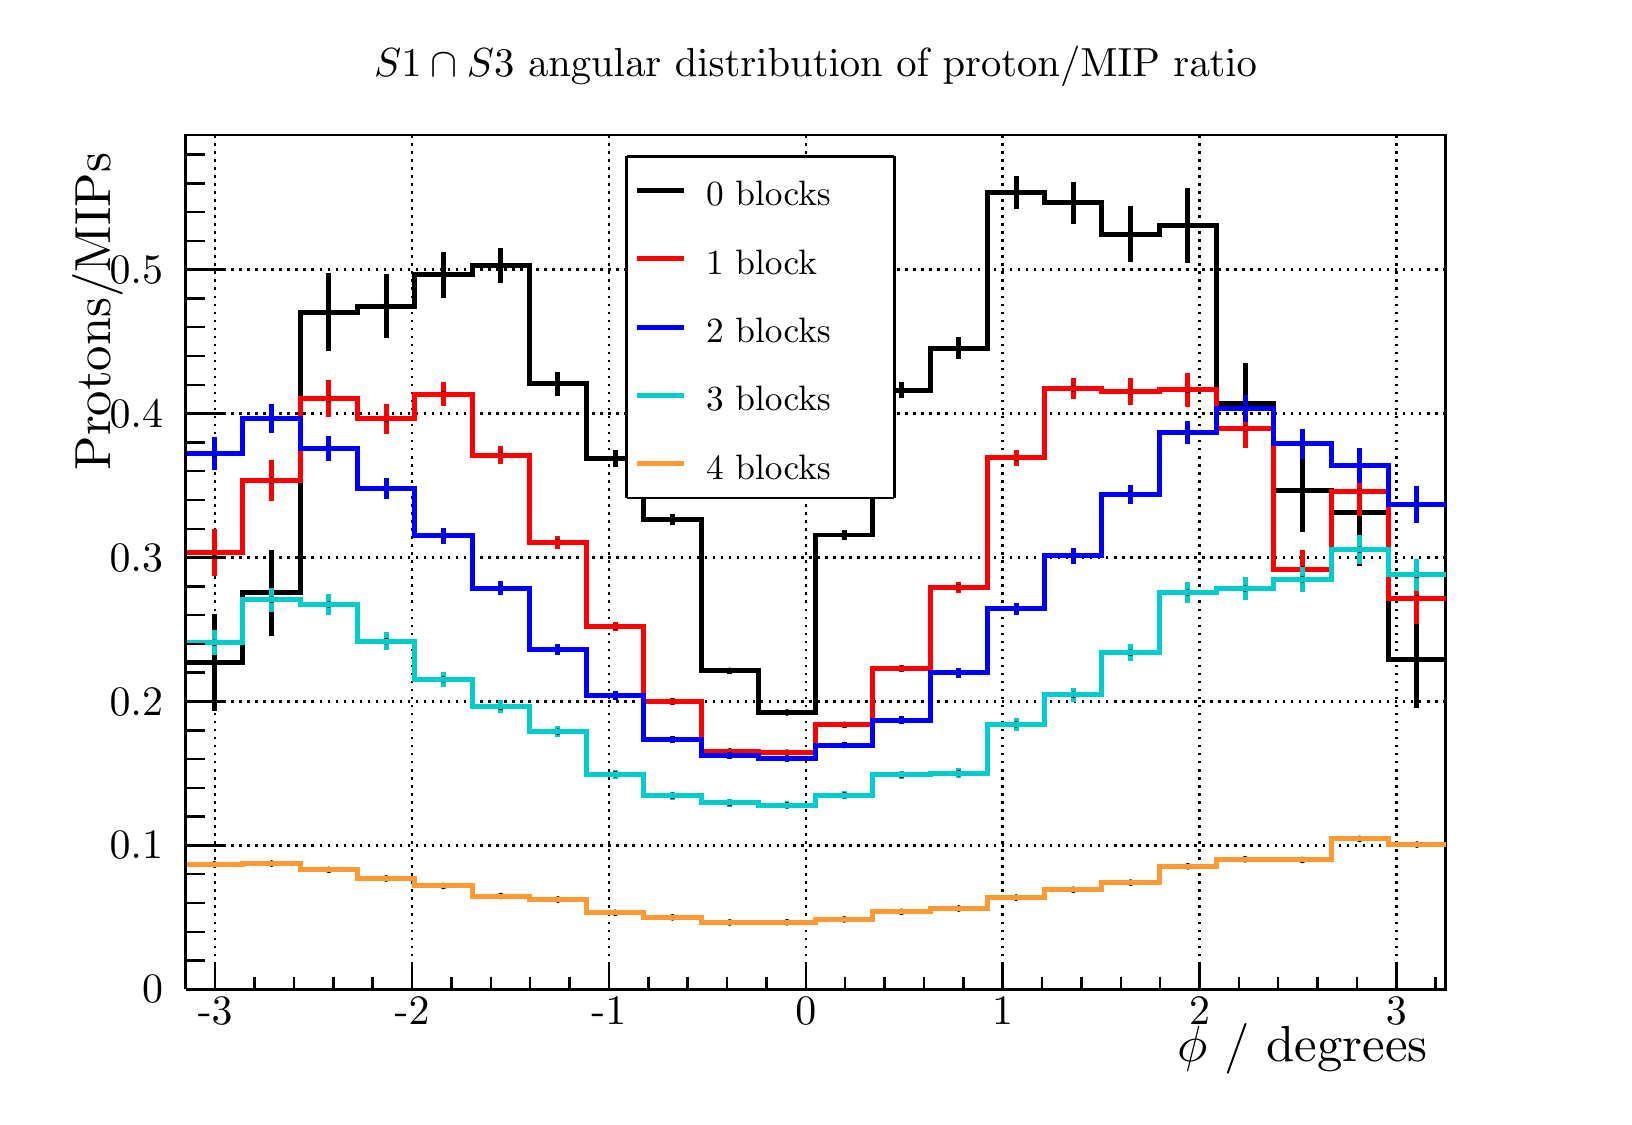
\begin{tikzpicture}
\pgfdeclareplotmark{cross} {
\pgfpathmoveto{\pgfpoint{-0.3\pgfplotmarksize}{\pgfplotmarksize}}
\pgfpathlineto{\pgfpoint{+0.3\pgfplotmarksize}{\pgfplotmarksize}}
\pgfpathlineto{\pgfpoint{+0.3\pgfplotmarksize}{0.3\pgfplotmarksize}}
\pgfpathlineto{\pgfpoint{+1\pgfplotmarksize}{0.3\pgfplotmarksize}}
\pgfpathlineto{\pgfpoint{+1\pgfplotmarksize}{-0.3\pgfplotmarksize}}
\pgfpathlineto{\pgfpoint{+0.3\pgfplotmarksize}{-0.3\pgfplotmarksize}}
\pgfpathlineto{\pgfpoint{+0.3\pgfplotmarksize}{-1.\pgfplotmarksize}}
\pgfpathlineto{\pgfpoint{-0.3\pgfplotmarksize}{-1.\pgfplotmarksize}}
\pgfpathlineto{\pgfpoint{-0.3\pgfplotmarksize}{-0.3\pgfplotmarksize}}
\pgfpathlineto{\pgfpoint{-1.\pgfplotmarksize}{-0.3\pgfplotmarksize}}
\pgfpathlineto{\pgfpoint{-1.\pgfplotmarksize}{0.3\pgfplotmarksize}}
\pgfpathlineto{\pgfpoint{-0.3\pgfplotmarksize}{0.3\pgfplotmarksize}}
\pgfpathclose
\pgfusepathqstroke
}
\pgfdeclareplotmark{cross*} {
\pgfpathmoveto{\pgfpoint{-0.3\pgfplotmarksize}{\pgfplotmarksize}}
\pgfpathlineto{\pgfpoint{+0.3\pgfplotmarksize}{\pgfplotmarksize}}
\pgfpathlineto{\pgfpoint{+0.3\pgfplotmarksize}{0.3\pgfplotmarksize}}
\pgfpathlineto{\pgfpoint{+1\pgfplotmarksize}{0.3\pgfplotmarksize}}
\pgfpathlineto{\pgfpoint{+1\pgfplotmarksize}{-0.3\pgfplotmarksize}}
\pgfpathlineto{\pgfpoint{+0.3\pgfplotmarksize}{-0.3\pgfplotmarksize}}
\pgfpathlineto{\pgfpoint{+0.3\pgfplotmarksize}{-1.\pgfplotmarksize}}
\pgfpathlineto{\pgfpoint{-0.3\pgfplotmarksize}{-1.\pgfplotmarksize}}
\pgfpathlineto{\pgfpoint{-0.3\pgfplotmarksize}{-0.3\pgfplotmarksize}}
\pgfpathlineto{\pgfpoint{-1.\pgfplotmarksize}{-0.3\pgfplotmarksize}}
\pgfpathlineto{\pgfpoint{-1.\pgfplotmarksize}{0.3\pgfplotmarksize}}
\pgfpathlineto{\pgfpoint{-0.3\pgfplotmarksize}{0.3\pgfplotmarksize}}
\pgfpathclose
\pgfusepathqfillstroke
}
\pgfdeclareplotmark{newstar} {
\pgfpathmoveto{\pgfqpoint{0pt}{\pgfplotmarksize}}
\pgfpathlineto{\pgfqpointpolar{44}{0.5\pgfplotmarksize}}
\pgfpathlineto{\pgfqpointpolar{18}{\pgfplotmarksize}}
\pgfpathlineto{\pgfqpointpolar{-20}{0.5\pgfplotmarksize}}
\pgfpathlineto{\pgfqpointpolar{-54}{\pgfplotmarksize}}
\pgfpathlineto{\pgfqpointpolar{-90}{0.5\pgfplotmarksize}}
\pgfpathlineto{\pgfqpointpolar{234}{\pgfplotmarksize}}
\pgfpathlineto{\pgfqpointpolar{198}{0.5\pgfplotmarksize}}
\pgfpathlineto{\pgfqpointpolar{162}{\pgfplotmarksize}}
\pgfpathlineto{\pgfqpointpolar{134}{0.5\pgfplotmarksize}}
\pgfpathclose
\pgfusepathqstroke
}
\pgfdeclareplotmark{newstar*} {
\pgfpathmoveto{\pgfqpoint{0pt}{\pgfplotmarksize}}
\pgfpathlineto{\pgfqpointpolar{44}{0.5\pgfplotmarksize}}
\pgfpathlineto{\pgfqpointpolar{18}{\pgfplotmarksize}}
\pgfpathlineto{\pgfqpointpolar{-20}{0.5\pgfplotmarksize}}
\pgfpathlineto{\pgfqpointpolar{-54}{\pgfplotmarksize}}
\pgfpathlineto{\pgfqpointpolar{-90}{0.5\pgfplotmarksize}}
\pgfpathlineto{\pgfqpointpolar{234}{\pgfplotmarksize}}
\pgfpathlineto{\pgfqpointpolar{198}{0.5\pgfplotmarksize}}
\pgfpathlineto{\pgfqpointpolar{162}{\pgfplotmarksize}}
\pgfpathlineto{\pgfqpointpolar{134}{0.5\pgfplotmarksize}}
\pgfpathclose
\pgfusepathqfillstroke
}
\definecolor{c}{rgb}{1,1,1};
\draw [color=c, fill=c] (0,0) rectangle (20,13.5632);
\draw [color=c, fill=c] (2,1.35632) rectangle (18,12.2069);
\definecolor{c}{rgb}{0,0,0};
\draw [c,line width=0.9] (2,1.35632) -- (2,12.2069) -- (18,12.2069) -- (18,1.35632) -- (2,1.35632);
\definecolor{c}{rgb}{1,1,1};
\draw [color=c, fill=c] (2,1.35632) rectangle (18,12.2069);
\definecolor{c}{rgb}{0,0,0};
\draw [c,line width=0.9] (2,1.35632) -- (2,12.2069) -- (18,12.2069) -- (18,1.35632) -- (2,1.35632);
\draw [c,line width=0.9] (2,1.35632) -- (18,1.35632);
\draw [c,dotted,line width=0.9] (2.375,12.2069) -- (2.375,1.35632);
\draw [c,dotted,line width=0.9] (4.875,12.2069) -- (4.875,1.35632);
\draw [c,dotted,line width=0.9] (7.375,12.2069) -- (7.375,1.35632);
\draw [c,dotted,line width=0.9] (9.875,12.2069) -- (9.875,1.35632);
\draw [c,dotted,line width=0.9] (12.375,12.2069) -- (12.375,1.35632);
\draw [c,dotted,line width=0.9] (14.875,12.2069) -- (14.875,1.35632);
\draw [c,dotted,line width=0.9] (17.375,12.2069) -- (17.375,1.35632);
\draw [c,dotted,line width=0.9] (2.375,12.2069) -- (2.375,1.35632);
\draw [c,dotted,line width=0.9] (17.375,12.2069) -- (17.375,1.35632);
\draw [c,line width=0.9] (2,1.35632) -- (2,12.2069);
\draw [c,dotted,line width=0.9] (18,1.35632) -- (2,1.35632);
\draw [c,dotted,line width=0.9] (18,3.18443) -- (2,3.18443);
\draw [c,dotted,line width=0.9] (18,5.01255) -- (2,5.01255);
\draw [c,dotted,line width=0.9] (18,6.84066) -- (2,6.84066);
\draw [c,dotted,line width=0.9] (18,8.66877) -- (2,8.66877);
\draw [c,dotted,line width=0.9] (18,10.4969) -- (2,10.4969);
\draw [c,dotted,line width=0.9] (18,10.4969) -- (2,10.4969);
\definecolor{c}{rgb}{0,0,0.6};
\draw [c,line width=0.9] (2,1.35632) -- (2.72727,1.35632) -- (2.72727,1.35632) -- (3.45455,1.35632) -- (3.45455,1.35632) -- (4.18182,1.35632) -- (4.18182,1.35632) -- (4.90909,1.35632) -- (4.90909,1.35632) -- (5.63636,1.35632) -- (5.63636,1.35632) --
 (6.36364,1.35632) -- (6.36364,1.35632) -- (7.09091,1.35632) -- (7.09091,1.35632) -- (7.81818,1.35632) -- (7.81818,1.35632) -- (8.54545,1.35632) -- (8.54545,1.35632) -- (9.27273,1.35632) -- (9.27273,1.35632) -- (10,1.35632) -- (10,1.35632) --
 (10.7273,1.35632) -- (10.7273,1.35632) -- (11.4545,1.35632) -- (11.4545,1.35632) -- (12.1818,1.35632) -- (12.1818,1.35632) -- (12.9091,1.35632) -- (12.9091,1.35632) -- (13.6364,1.35632) -- (13.6364,1.35632) -- (14.3636,1.35632) -- (14.3636,1.35632)
 -- (15.0909,1.35632) -- (15.0909,1.35632) -- (15.8182,1.35632) -- (15.8182,1.35632) -- (16.5455,1.35632) -- (16.5455,1.35632) -- (17.2727,1.35632) -- (17.2727,1.35632) -- (18,1.35632);
\definecolor{c}{rgb}{0,0,0};
\draw [c,line width=0.9] (2,1.35632) -- (18,1.35632);
\draw [anchor= east] (18,0.596782) node[scale=1.8317, color=c, rotate=0]{$\phi$ / degrees};
\draw [c,line width=0.9] (2.375,1.68184) -- (2.375,1.35632);
\draw [c,line width=0.9] (2.875,1.51908) -- (2.875,1.35632);
\draw [c,line width=0.9] (3.375,1.51908) -- (3.375,1.35632);
\draw [c,line width=0.9] (3.875,1.51908) -- (3.875,1.35632);
\draw [c,line width=0.9] (4.375,1.51908) -- (4.375,1.35632);
\draw [c,line width=0.9] (4.875,1.68184) -- (4.875,1.35632);
\draw [c,line width=0.9] (5.375,1.51908) -- (5.375,1.35632);
\draw [c,line width=0.9] (5.875,1.51908) -- (5.875,1.35632);
\draw [c,line width=0.9] (6.375,1.51908) -- (6.375,1.35632);
\draw [c,line width=0.9] (6.875,1.51908) -- (6.875,1.35632);
\draw [c,line width=0.9] (7.375,1.68184) -- (7.375,1.35632);
\draw [c,line width=0.9] (7.875,1.51908) -- (7.875,1.35632);
\draw [c,line width=0.9] (8.375,1.51908) -- (8.375,1.35632);
\draw [c,line width=0.9] (8.875,1.51908) -- (8.875,1.35632);
\draw [c,line width=0.9] (9.375,1.51908) -- (9.375,1.35632);
\draw [c,line width=0.9] (9.875,1.68184) -- (9.875,1.35632);
\draw [c,line width=0.9] (10.375,1.51908) -- (10.375,1.35632);
\draw [c,line width=0.9] (10.875,1.51908) -- (10.875,1.35632);
\draw [c,line width=0.9] (11.375,1.51908) -- (11.375,1.35632);
\draw [c,line width=0.9] (11.875,1.51908) -- (11.875,1.35632);
\draw [c,line width=0.9] (12.375,1.68184) -- (12.375,1.35632);
\draw [c,line width=0.9] (12.875,1.51908) -- (12.875,1.35632);
\draw [c,line width=0.9] (13.375,1.51908) -- (13.375,1.35632);
\draw [c,line width=0.9] (13.875,1.51908) -- (13.875,1.35632);
\draw [c,line width=0.9] (14.375,1.51908) -- (14.375,1.35632);
\draw [c,line width=0.9] (14.875,1.68184) -- (14.875,1.35632);
\draw [c,line width=0.9] (15.375,1.51908) -- (15.375,1.35632);
\draw [c,line width=0.9] (15.875,1.51908) -- (15.875,1.35632);
\draw [c,line width=0.9] (16.375,1.51908) -- (16.375,1.35632);
\draw [c,line width=0.9] (16.875,1.51908) -- (16.875,1.35632);
\draw [c,line width=0.9] (17.375,1.68184) -- (17.375,1.35632);
\draw [c,line width=0.9] (2.375,1.68184) -- (2.375,1.35632);
\draw [c,line width=0.9] (17.375,1.68184) -- (17.375,1.35632);
\draw [c,line width=0.9] (17.875,1.51908) -- (17.875,1.35632);
\draw [anchor=base] (2.375,0.908736) node[scale=1.5137, color=c, rotate=0]{-3};
\draw [anchor=base] (4.875,0.908736) node[scale=1.5137, color=c, rotate=0]{-2};
\draw [anchor=base] (7.375,0.908736) node[scale=1.5137, color=c, rotate=0]{-1};
\draw [anchor=base] (9.875,0.908736) node[scale=1.5137, color=c, rotate=0]{0};
\draw [anchor=base] (12.375,0.908736) node[scale=1.5137, color=c, rotate=0]{1};
\draw [anchor=base] (14.875,0.908736) node[scale=1.5137, color=c, rotate=0]{2};
\draw [anchor=base] (17.375,0.908736) node[scale=1.5137, color=c, rotate=0]{3};
\draw [c,line width=0.9] (2,1.35632) -- (2,12.2069);
\draw [anchor= east] (0.88,12.2069) node[scale=1.8317, color=c, rotate=90]{  Protons/MIPs};
\draw [c,line width=0.9] (2.48,1.35632) -- (2,1.35632);
\draw [c,line width=0.9] (2.24,1.72194) -- (2,1.72194);
\draw [c,line width=0.9] (2.24,2.08757) -- (2,2.08757);
\draw [c,line width=0.9] (2.24,2.45319) -- (2,2.45319);
\draw [c,line width=0.9] (2.24,2.81881) -- (2,2.81881);
\draw [c,line width=0.9] (2.48,3.18443) -- (2,3.18443);
\draw [c,line width=0.9] (2.24,3.55006) -- (2,3.55006);
\draw [c,line width=0.9] (2.24,3.91568) -- (2,3.91568);
\draw [c,line width=0.9] (2.24,4.2813) -- (2,4.2813);
\draw [c,line width=0.9] (2.24,4.64692) -- (2,4.64692);
\draw [c,line width=0.9] (2.48,5.01255) -- (2,5.01255);
\draw [c,line width=0.9] (2.24,5.37817) -- (2,5.37817);
\draw [c,line width=0.9] (2.24,5.74379) -- (2,5.74379);
\draw [c,line width=0.9] (2.24,6.10941) -- (2,6.10941);
\draw [c,line width=0.9] (2.24,6.47504) -- (2,6.47504);
\draw [c,line width=0.9] (2.48,6.84066) -- (2,6.84066);
\draw [c,line width=0.9] (2.24,7.20628) -- (2,7.20628);
\draw [c,line width=0.9] (2.24,7.5719) -- (2,7.5719);
\draw [c,line width=0.9] (2.24,7.93753) -- (2,7.93753);
\draw [c,line width=0.9] (2.24,8.30315) -- (2,8.30315);
\draw [c,line width=0.9] (2.48,8.66877) -- (2,8.66877);
\draw [c,line width=0.9] (2.24,9.03439) -- (2,9.03439);
\draw [c,line width=0.9] (2.24,9.40002) -- (2,9.40002);
\draw [c,line width=0.9] (2.24,9.76564) -- (2,9.76564);
\draw [c,line width=0.9] (2.24,10.1313) -- (2,10.1313);
\draw [c,line width=0.9] (2.48,10.4969) -- (2,10.4969);
\draw [c,line width=0.9] (2.48,10.4969) -- (2,10.4969);
\draw [c,line width=0.9] (2.24,10.8625) -- (2,10.8625);
\draw [c,line width=0.9] (2.24,11.2281) -- (2,11.2281);
\draw [c,line width=0.9] (2.24,11.5938) -- (2,11.5938);
\draw [c,line width=0.9] (2.24,11.9594) -- (2,11.9594);
\draw [anchor= east] (1.9,1.35632) node[scale=1.5137, color=c, rotate=0]{0};
\draw [anchor= east] (1.9,3.18443) node[scale=1.5137, color=c, rotate=0]{0.1};
\draw [anchor= east] (1.9,5.01255) node[scale=1.5137, color=c, rotate=0]{0.2};
\draw [anchor= east] (1.9,6.84066) node[scale=1.5137, color=c, rotate=0]{0.3};
\draw [anchor= east] (1.9,8.66877) node[scale=1.5137, color=c, rotate=0]{0.4};
\draw [anchor= east] (1.9,10.4969) node[scale=1.5137, color=c, rotate=0]{0.5};
\draw [c,line width=1.8] (2.36364,4.89378) -- (2.36364,5.51112);
\draw [c,line width=1.8] (2.36364,5.51112) -- (2.36364,6.12847);
\foreach \P in {(2.36364,5.51112)}{\draw[mark options={color=c,fill=c},mark size=2.402402pt,mark=*,mark size=1pt] plot coordinates {\P};}
\draw [c,line width=1.8] (3.09091,5.84926) -- (3.09091,6.39379);
\draw [c,line width=1.8] (3.09091,6.39379) -- (3.09091,6.93831);
\foreach \P in {(3.09091,6.39379)}{\draw[mark options={color=c,fill=c},mark size=2.402402pt,mark=*,mark size=1pt] plot coordinates {\P};}
\draw [c,line width=1.8] (3.81818,9.45971) -- (3.81818,9.95602);
\draw [c,line width=1.8] (3.81818,9.95602) -- (3.81818,10.4523);
\foreach \P in {(3.81818,9.95602)}{\draw[mark options={color=c,fill=c},mark size=2.402402pt,mark=*,mark size=1pt] plot coordinates {\P};}
\draw [c,line width=1.8] (4.54545,9.62928) -- (4.54545,10.0327);
\draw [c,line width=1.8] (4.54545,10.0327) -- (4.54545,10.4362);
\foreach \P in {(4.54545,10.0327)}{\draw[mark options={color=c,fill=c},mark size=2.402402pt,mark=*,mark size=1pt] plot coordinates {\P};}
\draw [c,line width=1.8] (5.27273,10.1359) -- (5.27273,10.4304);
\draw [c,line width=1.8] (5.27273,10.4304) -- (5.27273,10.725);
\foreach \P in {(5.27273,10.4304)}{\draw[mark options={color=c,fill=c},mark size=2.402402pt,mark=*,mark size=1pt] plot coordinates {\P};}
\draw [c,line width=1.8] (6,10.3215) -- (6,10.547);
\draw [c,line width=1.8] (6,10.547) -- (6,10.7725);
\foreach \P in {(6,10.547)}{\draw[mark options={color=c,fill=c},mark size=2.402402pt,mark=*,mark size=1pt] plot coordinates {\P};}
\draw [c,line width=1.8] (6.72727,8.89213) -- (6.72727,9.04764);
\draw [c,line width=1.8] (6.72727,9.04764) -- (6.72727,9.20315);
\foreach \P in {(6.72727,9.04764)}{\draw[mark options={color=c,fill=c},mark size=2.402402pt,mark=*,mark size=1pt] plot coordinates {\P};}
\draw [c,line width=1.8] (7.45455,7.99309) -- (7.45455,8.09945);
\draw [c,line width=1.8] (7.45455,8.09945) -- (7.45455,8.2058);
\foreach \P in {(7.45455,8.09945)}{\draw[mark options={color=c,fill=c},mark size=2.402402pt,mark=*,mark size=1pt] plot coordinates {\P};}
\draw [c,line width=1.8] (8.18182,7.25752) -- (8.18182,7.3273);
\draw [c,line width=1.8] (8.18182,7.3273) -- (8.18182,7.39708);
\foreach \P in {(8.18182,7.3273)}{\draw[mark options={color=c,fill=c},mark size=2.402402pt,mark=*,mark size=1pt] plot coordinates {\P};}
\draw [c,line width=1.8] (8.90909,5.36598) -- (8.90909,5.40179);
\draw [c,line width=1.8] (8.90909,5.40179) -- (8.90909,5.4376);
\foreach \P in {(8.90909,5.40179)}{\draw[mark options={color=c,fill=c},mark size=2.402402pt,mark=*,mark size=1pt] plot coordinates {\P};}
\draw [c,line width=1.8] (9.63636,4.84341) -- (9.63636,4.87303);
\draw [c,line width=1.8] (9.63636,4.87303) -- (9.63636,4.90264);
\foreach \P in {(9.63636,4.87303)}{\draw[mark options={color=c,fill=c},mark size=2.402402pt,mark=*,mark size=1pt] plot coordinates {\P};}
\draw [c,line width=1.8] (10.3636,7.06938) -- (10.3636,7.12713);
\draw [c,line width=1.8] (10.3636,7.12713) -- (10.3636,7.18488);
\foreach \P in {(10.3636,7.12713)}{\draw[mark options={color=c,fill=c},mark size=2.402402pt,mark=*,mark size=1pt] plot coordinates {\P};}
\draw [c,line width=1.8] (11.0909,8.86292) -- (11.0909,8.96454);
\draw [c,line width=1.8] (11.0909,8.96454) -- (11.0909,9.06617);
\foreach \P in {(11.0909,8.96454)}{\draw[mark options={color=c,fill=c},mark size=2.402402pt,mark=*,mark size=1pt] plot coordinates {\P};}
\draw [c,line width=1.8] (11.8182,9.36011) -- (11.8182,9.50073);
\draw [c,line width=1.8] (11.8182,9.50073) -- (11.8182,9.64135);
\foreach \P in {(11.8182,9.50073)}{\draw[mark options={color=c,fill=c},mark size=2.402402pt,mark=*,mark size=1pt] plot coordinates {\P};}
\draw [c,line width=1.8] (12.5455,11.263) -- (12.5455,11.4766);
\draw [c,line width=1.8] (12.5455,11.4766) -- (12.5455,11.6902);
\foreach \P in {(12.5455,11.4766)}{\draw[mark options={color=c,fill=c},mark size=2.402402pt,mark=*,mark size=1pt] plot coordinates {\P};}
\draw [c,line width=1.8] (13.2727,11.0759) -- (13.2727,11.3437);
\draw [c,line width=1.8] (13.2727,11.3437) -- (13.2727,11.6115);
\foreach \P in {(13.2727,11.3437)}{\draw[mark options={color=c,fill=c},mark size=2.402402pt,mark=*,mark size=1pt] plot coordinates {\P};}
\draw [c,line width=1.8] (14,10.588) -- (14,10.9455);
\draw [c,line width=1.8] (14,10.9455) -- (14,11.303);
\foreach \P in {(14,10.9455)}{\draw[mark options={color=c,fill=c},mark size=2.402402pt,mark=*,mark size=1pt] plot coordinates {\P};}
\draw [c,line width=1.8] (14.7273,10.5864) -- (14.7273,11.0575);
\draw [c,line width=1.8] (14.7273,11.0575) -- (14.7273,11.5286);
\foreach \P in {(14.7273,11.0575)}{\draw[mark options={color=c,fill=c},mark size=2.402402pt,mark=*,mark size=1pt] plot coordinates {\P};}
\draw [c,line width=1.8] (15.4545,8.28922) -- (15.4545,8.79768);
\draw [c,line width=1.8] (15.4545,8.79768) -- (15.4545,9.30614);
\foreach \P in {(15.4545,8.79768)}{\draw[mark options={color=c,fill=c},mark size=2.402402pt,mark=*,mark size=1pt] plot coordinates {\P};}
\draw [c,line width=1.8] (16.1818,7.16906) -- (16.1818,7.69467);
\draw [c,line width=1.8] (16.1818,7.69467) -- (16.1818,8.22028);
\foreach \P in {(16.1818,7.69467)}{\draw[mark options={color=c,fill=c},mark size=2.402402pt,mark=*,mark size=1pt] plot coordinates {\P};}
\draw [c,line width=1.8] (16.9091,6.73172) -- (16.9091,7.41194);
\draw [c,line width=1.8] (16.9091,7.41194) -- (16.9091,8.09217);
\foreach \P in {(16.9091,7.41194)}{\draw[mark options={color=c,fill=c},mark size=2.402402pt,mark=*,mark size=1pt] plot coordinates {\P};}
\draw [c,line width=1.8] (17.6364,4.93484) -- (17.6364,5.54817);
\draw [c,line width=1.8] (17.6364,5.54817) -- (17.6364,6.16151);
\foreach \P in {(17.6364,5.54817)}{\draw[mark options={color=c,fill=c},mark size=2.402402pt,mark=*,mark size=1pt] plot coordinates {\P};}
\draw [c,line width=1.8] (2,5.51112) -- (2.72727,5.51112) -- (2.72727,6.39379) -- (3.45455,6.39379) -- (3.45455,9.95602) -- (4.18182,9.95602) -- (4.18182,10.0327) -- (4.90909,10.0327) -- (4.90909,10.4304) -- (5.63636,10.4304) -- (5.63636,10.547) --
 (6.36364,10.547) -- (6.36364,9.04764) -- (7.09091,9.04764) -- (7.09091,8.09945) -- (7.81818,8.09945) -- (7.81818,7.3273) -- (8.54545,7.3273) -- (8.54545,5.40179) -- (9.27273,5.40179) -- (9.27273,4.87303) -- (10,4.87303) -- (10,7.12713) --
 (10.7273,7.12713) -- (10.7273,8.96454) -- (11.4545,8.96454) -- (11.4545,9.50073) -- (12.1818,9.50073) -- (12.1818,11.4766) -- (12.9091,11.4766) -- (12.9091,11.3437) -- (13.6364,11.3437) -- (13.6364,10.9455) -- (14.3636,10.9455) -- (14.3636,11.0575)
 -- (15.0909,11.0575) -- (15.0909,8.79768) -- (15.8182,8.79768) -- (15.8182,7.69467) -- (16.5455,7.69467) -- (16.5455,7.41194) -- (17.2727,7.41194) -- (17.2727,5.54817) -- (18,5.54817);
\definecolor{c}{rgb}{1,0,0};
\draw [c,line width=1.8] (2.36364,6.60423) -- (2.36364,6.90306);
\draw [c,line width=1.8] (2.36364,6.90306) -- (2.36364,7.20189);
\definecolor{c}{rgb}{0,0,0};
\foreach \P in {(2.36364,6.90306)}{\draw[mark options={color=c,fill=c},mark size=2.402402pt,mark=*,mark size=1pt] plot coordinates {\P};}
\definecolor{c}{rgb}{1,0,0};
\draw [c,line width=1.8] (3.09091,7.5545) -- (3.09091,7.8162);
\draw [c,line width=1.8] (3.09091,7.8162) -- (3.09091,8.0779);
\definecolor{c}{rgb}{0,0,0};
\foreach \P in {(3.09091,7.8162)}{\draw[mark options={color=c,fill=c},mark size=2.402402pt,mark=*,mark size=1pt] plot coordinates {\P};}
\definecolor{c}{rgb}{1,0,0};
\draw [c,line width=1.8] (3.81818,8.62873) -- (3.81818,8.86031);
\draw [c,line width=1.8] (3.81818,8.86031) -- (3.81818,9.09189);
\definecolor{c}{rgb}{0,0,0};
\foreach \P in {(3.81818,8.86031)}{\draw[mark options={color=c,fill=c},mark size=2.402402pt,mark=*,mark size=1pt] plot coordinates {\P};}
\definecolor{c}{rgb}{1,0,0};
\draw [c,line width=1.8] (4.54545,8.41495) -- (4.54545,8.60083);
\draw [c,line width=1.8] (4.54545,8.60083) -- (4.54545,8.78671);
\definecolor{c}{rgb}{0,0,0};
\foreach \P in {(4.54545,8.60083)}{\draw[mark options={color=c,fill=c},mark size=2.402402pt,mark=*,mark size=1pt] plot coordinates {\P};}
\definecolor{c}{rgb}{1,0,0};
\draw [c,line width=1.8] (5.27273,8.76828) -- (5.27273,8.91648);
\draw [c,line width=1.8] (5.27273,8.91648) -- (5.27273,9.06469);
\definecolor{c}{rgb}{0,0,0};
\foreach \P in {(5.27273,8.91648)}{\draw[mark options={color=c,fill=c},mark size=2.402402pt,mark=*,mark size=1pt] plot coordinates {\P};}
\definecolor{c}{rgb}{1,0,0};
\draw [c,line width=1.8] (6,8.02779) -- (6,8.14192);
\draw [c,line width=1.8] (6,8.14192) -- (6,8.25604);
\definecolor{c}{rgb}{0,0,0};
\foreach \P in {(6,8.14192)}{\draw[mark options={color=c,fill=c},mark size=2.402402pt,mark=*,mark size=1pt] plot coordinates {\P};}
\definecolor{c}{rgb}{1,0,0};
\draw [c,line width=1.8] (6.72727,6.95442) -- (6.72727,7.03619);
\draw [c,line width=1.8] (6.72727,7.03619) -- (6.72727,7.11796);
\definecolor{c}{rgb}{0,0,0};
\foreach \P in {(6.72727,7.03619)}{\draw[mark options={color=c,fill=c},mark size=2.402402pt,mark=*,mark size=1pt] plot coordinates {\P};}
\definecolor{c}{rgb}{1,0,0};
\draw [c,line width=1.8] (7.45455,5.90288) -- (7.45455,5.96141);
\draw [c,line width=1.8] (7.45455,5.96141) -- (7.45455,6.01994);
\definecolor{c}{rgb}{0,0,0};
\foreach \P in {(7.45455,5.96141)}{\draw[mark options={color=c,fill=c},mark size=2.402402pt,mark=*,mark size=1pt] plot coordinates {\P};}
\definecolor{c}{rgb}{1,0,0};
\draw [c,line width=1.8] (8.18182,4.97126) -- (8.18182,5.01446);
\draw [c,line width=1.8] (8.18182,5.01446) -- (8.18182,5.05766);
\definecolor{c}{rgb}{0,0,0};
\foreach \P in {(8.18182,5.01446)}{\draw[mark options={color=c,fill=c},mark size=2.402402pt,mark=*,mark size=1pt] plot coordinates {\P};}
\definecolor{c}{rgb}{1,0,0};
\draw [c,line width=1.8] (8.90909,4.34427) -- (8.90909,4.37898);
\draw [c,line width=1.8] (8.90909,4.37898) -- (8.90909,4.41369);
\definecolor{c}{rgb}{0,0,0};
\foreach \P in {(8.90909,4.37898)}{\draw[mark options={color=c,fill=c},mark size=2.402402pt,mark=*,mark size=1pt] plot coordinates {\P};}
\definecolor{c}{rgb}{1,0,0};
\draw [c,line width=1.8] (9.63636,4.32923) -- (9.63636,4.3633);
\draw [c,line width=1.8] (9.63636,4.3633) -- (9.63636,4.39736);
\definecolor{c}{rgb}{0,0,0};
\foreach \P in {(9.63636,4.3633)}{\draw[mark options={color=c,fill=c},mark size=2.402402pt,mark=*,mark size=1pt] plot coordinates {\P};}
\definecolor{c}{rgb}{1,0,0};
\draw [c,line width=1.8] (10.3636,4.67726) -- (10.3636,4.71602);
\draw [c,line width=1.8] (10.3636,4.71602) -- (10.3636,4.75479);
\definecolor{c}{rgb}{0,0,0};
\foreach \P in {(10.3636,4.71602)}{\draw[mark options={color=c,fill=c},mark size=2.402402pt,mark=*,mark size=1pt] plot coordinates {\P};}
\definecolor{c}{rgb}{1,0,0};
\draw [c,line width=1.8] (11.0909,5.38166) -- (11.0909,5.43154);
\draw [c,line width=1.8] (11.0909,5.43154) -- (11.0909,5.48143);
\definecolor{c}{rgb}{0,0,0};
\foreach \P in {(11.0909,5.43154)}{\draw[mark options={color=c,fill=c},mark size=2.402402pt,mark=*,mark size=1pt] plot coordinates {\P};}
\definecolor{c}{rgb}{1,0,0};
\draw [c,line width=1.8] (11.8182,6.39514) -- (11.8182,6.46287);
\draw [c,line width=1.8] (11.8182,6.46287) -- (11.8182,6.5306);
\definecolor{c}{rgb}{0,0,0};
\foreach \P in {(11.8182,6.46287)}{\draw[mark options={color=c,fill=c},mark size=2.402402pt,mark=*,mark size=1pt] plot coordinates {\P};}
\definecolor{c}{rgb}{1,0,0};
\draw [c,line width=1.8] (12.5455,8.00437) -- (12.5455,8.10677);
\draw [c,line width=1.8] (12.5455,8.10677) -- (12.5455,8.20917);
\definecolor{c}{rgb}{0,0,0};
\foreach \P in {(12.5455,8.10677)}{\draw[mark options={color=c,fill=c},mark size=2.402402pt,mark=*,mark size=1pt] plot coordinates {\P};}
\definecolor{c}{rgb}{1,0,0};
\draw [c,line width=1.8] (13.2727,8.85335) -- (13.2727,8.98853);
\draw [c,line width=1.8] (13.2727,8.98853) -- (13.2727,9.1237);
\definecolor{c}{rgb}{0,0,0};
\foreach \P in {(13.2727,8.98853)}{\draw[mark options={color=c,fill=c},mark size=2.402402pt,mark=*,mark size=1pt] plot coordinates {\P};}
\definecolor{c}{rgb}{1,0,0};
\draw [c,line width=1.8] (14,8.77802) -- (14,8.94714);
\draw [c,line width=1.8] (14,8.94714) -- (14,9.11627);
\definecolor{c}{rgb}{0,0,0};
\foreach \P in {(14,8.94714)}{\draw[mark options={color=c,fill=c},mark size=2.402402pt,mark=*,mark size=1pt] plot coordinates {\P};}
\definecolor{c}{rgb}{1,0,0};
\draw [c,line width=1.8] (14.7273,8.75518) -- (14.7273,8.96999);
\draw [c,line width=1.8] (14.7273,8.96999) -- (14.7273,9.18481);
\definecolor{c}{rgb}{0,0,0};
\foreach \P in {(14.7273,8.96999)}{\draw[mark options={color=c,fill=c},mark size=2.402402pt,mark=*,mark size=1pt] plot coordinates {\P};}
\definecolor{c}{rgb}{1,0,0};
\draw [c,line width=1.8] (15.4545,8.23655) -- (15.4545,8.47919);
\draw [c,line width=1.8] (15.4545,8.47919) -- (15.4545,8.72183);
\definecolor{c}{rgb}{0,0,0};
\foreach \P in {(15.4545,8.47919)}{\draw[mark options={color=c,fill=c},mark size=2.402402pt,mark=*,mark size=1pt] plot coordinates {\P};}
\definecolor{c}{rgb}{1,0,0};
\draw [c,line width=1.8] (16.1818,6.44051) -- (16.1818,6.69109);
\draw [c,line width=1.8] (16.1818,6.69109) -- (16.1818,6.94166);
\definecolor{c}{rgb}{0,0,0};
\foreach \P in {(16.1818,6.69109)}{\draw[mark options={color=c,fill=c},mark size=2.402402pt,mark=*,mark size=1pt] plot coordinates {\P};}
\definecolor{c}{rgb}{1,0,0};
\draw [c,line width=1.8] (16.9091,7.36681) -- (16.9091,7.68164);
\draw [c,line width=1.8] (16.9091,7.68164) -- (16.9091,7.99646);
\definecolor{c}{rgb}{0,0,0};
\foreach \P in {(16.9091,7.68164)}{\draw[mark options={color=c,fill=c},mark size=2.402402pt,mark=*,mark size=1pt] plot coordinates {\P};}
\definecolor{c}{rgb}{1,0,0};
\draw [c,line width=1.8] (17.6364,5.99877) -- (17.6364,6.32595);
\draw [c,line width=1.8] (17.6364,6.32595) -- (17.6364,6.65312);
\definecolor{c}{rgb}{0,0,0};
\foreach \P in {(17.6364,6.32595)}{\draw[mark options={color=c,fill=c},mark size=2.402402pt,mark=*,mark size=1pt] plot coordinates {\P};}
\definecolor{c}{rgb}{1,0,0};
\draw [c,line width=1.8] (2,6.90306) -- (2.72727,6.90306) -- (2.72727,7.8162) -- (3.45455,7.8162) -- (3.45455,8.86031) -- (4.18182,8.86031) -- (4.18182,8.60083) -- (4.90909,8.60083) -- (4.90909,8.91648) -- (5.63636,8.91648) -- (5.63636,8.14192) --
 (6.36364,8.14192) -- (6.36364,7.03619) -- (7.09091,7.03619) -- (7.09091,5.96141) -- (7.81818,5.96141) -- (7.81818,5.01446) -- (8.54545,5.01446) -- (8.54545,4.37898) -- (9.27273,4.37898) -- (9.27273,4.3633) -- (10,4.3633) -- (10,4.71602) --
 (10.7273,4.71602) -- (10.7273,5.43154) -- (11.4545,5.43154) -- (11.4545,6.46287) -- (12.1818,6.46287) -- (12.1818,8.10677) -- (12.9091,8.10677) -- (12.9091,8.98853) -- (13.6364,8.98853) -- (13.6364,8.94714) -- (14.3636,8.94714) -- (14.3636,8.96999)
 -- (15.0909,8.96999) -- (15.0909,8.47919) -- (15.8182,8.47919) -- (15.8182,6.69109) -- (16.5455,6.69109) -- (16.5455,7.68164) -- (17.2727,7.68164) -- (17.2727,6.32595) -- (18,6.32595);
\definecolor{c}{rgb}{0,0,1};
\draw [c,line width=1.8] (2.36364,7.94927) -- (2.36364,8.15813);
\draw [c,line width=1.8] (2.36364,8.15813) -- (2.36364,8.36698);
\definecolor{c}{rgb}{0,0,0};
\foreach \P in {(2.36364,8.15813)}{\draw[mark options={color=c,fill=c},mark size=2.402402pt,mark=*,mark size=1pt] plot coordinates {\P};}
\definecolor{c}{rgb}{0,0,1};
\draw [c,line width=1.8] (3.09091,8.41768) -- (3.09091,8.60289);
\draw [c,line width=1.8] (3.09091,8.60289) -- (3.09091,8.78811);
\definecolor{c}{rgb}{0,0,0};
\foreach \P in {(3.09091,8.60289)}{\draw[mark options={color=c,fill=c},mark size=2.402402pt,mark=*,mark size=1pt] plot coordinates {\P};}
\definecolor{c}{rgb}{0,0,1};
\draw [c,line width=1.8] (3.81818,8.07214) -- (3.81818,8.23082);
\draw [c,line width=1.8] (3.81818,8.23082) -- (3.81818,8.38951);
\definecolor{c}{rgb}{0,0,0};
\foreach \P in {(3.81818,8.23082)}{\draw[mark options={color=c,fill=c},mark size=2.402402pt,mark=*,mark size=1pt] plot coordinates {\P};}
\definecolor{c}{rgb}{0,0,1};
\draw [c,line width=1.8] (4.54545,7.58374) -- (4.54545,7.71608);
\draw [c,line width=1.8] (4.54545,7.71608) -- (4.54545,7.84841);
\definecolor{c}{rgb}{0,0,0};
\foreach \P in {(4.54545,7.71608)}{\draw[mark options={color=c,fill=c},mark size=2.402402pt,mark=*,mark size=1pt] plot coordinates {\P};}
\definecolor{c}{rgb}{0,0,1};
\draw [c,line width=1.8] (5.27273,7.0098) -- (5.27273,7.11593);
\draw [c,line width=1.8] (5.27273,7.11593) -- (5.27273,7.22207);
\definecolor{c}{rgb}{0,0,0};
\foreach \P in {(5.27273,7.11593)}{\draw[mark options={color=c,fill=c},mark size=2.402402pt,mark=*,mark size=1pt] plot coordinates {\P};}
\definecolor{c}{rgb}{0,0,1};
\draw [c,line width=1.8] (6,6.36486) -- (6,6.45215);
\draw [c,line width=1.8] (6,6.45215) -- (6,6.53944);
\definecolor{c}{rgb}{0,0,0};
\foreach \P in {(6,6.45215)}{\draw[mark options={color=c,fill=c},mark size=2.402402pt,mark=*,mark size=1pt] plot coordinates {\P};}
\definecolor{c}{rgb}{0,0,1};
\draw [c,line width=1.8] (6.72727,5.60459) -- (6.72727,5.67248);
\draw [c,line width=1.8] (6.72727,5.67248) -- (6.72727,5.74038);
\definecolor{c}{rgb}{0,0,0};
\foreach \P in {(6.72727,5.67248)}{\draw[mark options={color=c,fill=c},mark size=2.402402pt,mark=*,mark size=1pt] plot coordinates {\P};}
\definecolor{c}{rgb}{0,0,1};
\draw [c,line width=1.8] (7.45455,5.03204) -- (7.45455,5.08687);
\draw [c,line width=1.8] (7.45455,5.08687) -- (7.45455,5.14171);
\definecolor{c}{rgb}{0,0,0};
\foreach \P in {(7.45455,5.08687)}{\draw[mark options={color=c,fill=c},mark size=2.402402pt,mark=*,mark size=1pt] plot coordinates {\P};}
\definecolor{c}{rgb}{0,0,1};
\draw [c,line width=1.8] (8.18182,4.4863) -- (8.18182,4.53181);
\draw [c,line width=1.8] (8.18182,4.53181) -- (8.18182,4.57731);
\definecolor{c}{rgb}{0,0,0};
\foreach \P in {(8.18182,4.53181)}{\draw[mark options={color=c,fill=c},mark size=2.402402pt,mark=*,mark size=1pt] plot coordinates {\P};}
\definecolor{c}{rgb}{0,0,1};
\draw [c,line width=1.8] (8.90909,4.287) -- (8.90909,4.32814);
\draw [c,line width=1.8] (8.90909,4.32814) -- (8.90909,4.36928);
\definecolor{c}{rgb}{0,0,0};
\foreach \P in {(8.90909,4.32814)}{\draw[mark options={color=c,fill=c},mark size=2.402402pt,mark=*,mark size=1pt] plot coordinates {\P};}
\definecolor{c}{rgb}{0,0,1};
\draw [c,line width=1.8] (9.63636,4.24632) -- (9.63636,4.28747);
\draw [c,line width=1.8] (9.63636,4.28747) -- (9.63636,4.32862);
\definecolor{c}{rgb}{0,0,0};
\foreach \P in {(9.63636,4.28747)}{\draw[mark options={color=c,fill=c},mark size=2.402402pt,mark=*,mark size=1pt] plot coordinates {\P};}
\definecolor{c}{rgb}{0,0,1};
\draw [c,line width=1.8] (10.3636,4.41574) -- (10.3636,4.45963);
\draw [c,line width=1.8] (10.3636,4.45963) -- (10.3636,4.50353);
\definecolor{c}{rgb}{0,0,0};
\foreach \P in {(10.3636,4.45963)}{\draw[mark options={color=c,fill=c},mark size=2.402402pt,mark=*,mark size=1pt] plot coordinates {\P};}
\definecolor{c}{rgb}{0,0,1};
\draw [c,line width=1.8] (11.0909,4.72467) -- (11.0909,4.77477);
\draw [c,line width=1.8] (11.0909,4.77477) -- (11.0909,4.82488);
\definecolor{c}{rgb}{0,0,0};
\foreach \P in {(11.0909,4.77477)}{\draw[mark options={color=c,fill=c},mark size=2.402402pt,mark=*,mark size=1pt] plot coordinates {\P};}
\definecolor{c}{rgb}{0,0,1};
\draw [c,line width=1.8] (11.8182,5.31697) -- (11.8182,5.37768);
\draw [c,line width=1.8] (11.8182,5.37768) -- (11.8182,5.43838);
\definecolor{c}{rgb}{0,0,0};
\foreach \P in {(11.8182,5.37768)}{\draw[mark options={color=c,fill=c},mark size=2.402402pt,mark=*,mark size=1pt] plot coordinates {\P};}
\definecolor{c}{rgb}{0,0,1};
\draw [c,line width=1.8] (12.5455,6.10984) -- (12.5455,6.18951);
\draw [c,line width=1.8] (12.5455,6.18951) -- (12.5455,6.26918);
\definecolor{c}{rgb}{0,0,0};
\foreach \P in {(12.5455,6.18951)}{\draw[mark options={color=c,fill=c},mark size=2.402402pt,mark=*,mark size=1pt] plot coordinates {\P};}
\definecolor{c}{rgb}{0,0,1};
\draw [c,line width=1.8] (13.2727,6.76253) -- (13.2727,6.862);
\draw [c,line width=1.8] (13.2727,6.862) -- (13.2727,6.96147);
\definecolor{c}{rgb}{0,0,0};
\foreach \P in {(13.2727,6.862)}{\draw[mark options={color=c,fill=c},mark size=2.402402pt,mark=*,mark size=1pt] plot coordinates {\P};}
\definecolor{c}{rgb}{0,0,1};
\draw [c,line width=1.8] (14,7.52013) -- (14,7.64309);
\draw [c,line width=1.8] (14,7.64309) -- (14,7.76606);
\definecolor{c}{rgb}{0,0,0};
\foreach \P in {(14,7.64309)}{\draw[mark options={color=c,fill=c},mark size=2.402402pt,mark=*,mark size=1pt] plot coordinates {\P};}
\definecolor{c}{rgb}{0,0,1};
\draw [c,line width=1.8] (14.7273,8.27652) -- (14.7273,8.42762);
\draw [c,line width=1.8] (14.7273,8.42762) -- (14.7273,8.57872);
\definecolor{c}{rgb}{0,0,0};
\foreach \P in {(14.7273,8.42762)}{\draw[mark options={color=c,fill=c},mark size=2.402402pt,mark=*,mark size=1pt] plot coordinates {\P};}
\definecolor{c}{rgb}{0,0,1};
\draw [c,line width=1.8] (15.4545,8.56516) -- (15.4545,8.73804);
\draw [c,line width=1.8] (15.4545,8.73804) -- (15.4545,8.91092);
\definecolor{c}{rgb}{0,0,0};
\foreach \P in {(15.4545,8.73804)}{\draw[mark options={color=c,fill=c},mark size=2.402402pt,mark=*,mark size=1pt] plot coordinates {\P};}
\definecolor{c}{rgb}{0,0,1};
\draw [c,line width=1.8] (16.1818,8.09282) -- (16.1818,8.28382);
\draw [c,line width=1.8] (16.1818,8.28382) -- (16.1818,8.47482);
\definecolor{c}{rgb}{0,0,0};
\foreach \P in {(16.1818,8.28382)}{\draw[mark options={color=c,fill=c},mark size=2.402402pt,mark=*,mark size=1pt] plot coordinates {\P};}
\definecolor{c}{rgb}{0,0,1};
\draw [c,line width=1.8] (16.9091,7.78327) -- (16.9091,8.00724);
\draw [c,line width=1.8] (16.9091,8.00724) -- (16.9091,8.23121);
\definecolor{c}{rgb}{0,0,0};
\foreach \P in {(16.9091,8.00724)}{\draw[mark options={color=c,fill=c},mark size=2.402402pt,mark=*,mark size=1pt] plot coordinates {\P};}
\definecolor{c}{rgb}{0,0,1};
\draw [c,line width=1.8] (17.6364,7.27676) -- (17.6364,7.51476);
\draw [c,line width=1.8] (17.6364,7.51476) -- (17.6364,7.75276);
\definecolor{c}{rgb}{0,0,0};
\foreach \P in {(17.6364,7.51476)}{\draw[mark options={color=c,fill=c},mark size=2.402402pt,mark=*,mark size=1pt] plot coordinates {\P};}
\definecolor{c}{rgb}{0,0,1};
\draw [c,line width=1.8] (2,8.15813) -- (2.72727,8.15813) -- (2.72727,8.60289) -- (3.45455,8.60289) -- (3.45455,8.23082) -- (4.18182,8.23082) -- (4.18182,7.71608) -- (4.90909,7.71608) -- (4.90909,7.11593) -- (5.63636,7.11593) -- (5.63636,6.45215) --
 (6.36364,6.45215) -- (6.36364,5.67248) -- (7.09091,5.67248) -- (7.09091,5.08687) -- (7.81818,5.08687) -- (7.81818,4.53181) -- (8.54545,4.53181) -- (8.54545,4.32814) -- (9.27273,4.32814) -- (9.27273,4.28747) -- (10,4.28747) -- (10,4.45963) --
 (10.7273,4.45963) -- (10.7273,4.77477) -- (11.4545,4.77477) -- (11.4545,5.37768) -- (12.1818,5.37768) -- (12.1818,6.18951) -- (12.9091,6.18951) -- (12.9091,6.862) -- (13.6364,6.862) -- (13.6364,7.64309) -- (14.3636,7.64309) -- (14.3636,8.42762) --
 (15.0909,8.42762) -- (15.0909,8.73804) -- (15.8182,8.73804) -- (15.8182,8.28382) -- (16.5455,8.28382) -- (16.5455,8.00724) -- (17.2727,8.00724) -- (17.2727,7.51476) -- (18,7.51476);
\definecolor{c}{rgb}{0,0.8,0.8};
\draw [c,line width=1.8] (2.36364,5.60065) -- (2.36364,5.75802);
\draw [c,line width=1.8] (2.36364,5.75802) -- (2.36364,5.91539);
\definecolor{c}{rgb}{0,0,0};
\foreach \P in {(2.36364,5.75802)}{\draw[mark options={color=c,fill=c},mark size=2.402402pt,mark=*,mark size=1pt] plot coordinates {\P};}
\definecolor{c}{rgb}{0,0.8,0.8};
\draw [c,line width=1.8] (3.09091,6.15354) -- (3.09091,6.30546);
\draw [c,line width=1.8] (3.09091,6.30546) -- (3.09091,6.45738);
\definecolor{c}{rgb}{0,0,0};
\foreach \P in {(3.09091,6.30546)}{\draw[mark options={color=c,fill=c},mark size=2.402402pt,mark=*,mark size=1pt] plot coordinates {\P};}
\definecolor{c}{rgb}{0,0.8,0.8};
\draw [c,line width=1.8] (3.81818,6.10854) -- (3.81818,6.24391);
\draw [c,line width=1.8] (3.81818,6.24391) -- (3.81818,6.37929);
\definecolor{c}{rgb}{0,0,0};
\foreach \P in {(3.81818,6.24391)}{\draw[mark options={color=c,fill=c},mark size=2.402402pt,mark=*,mark size=1pt] plot coordinates {\P};}
\definecolor{c}{rgb}{0,0.8,0.8};
\draw [c,line width=1.8] (4.54545,5.66395) -- (4.54545,5.77943);
\draw [c,line width=1.8] (4.54545,5.77943) -- (4.54545,5.89492);
\definecolor{c}{rgb}{0,0,0};
\foreach \P in {(4.54545,5.77943)}{\draw[mark options={color=c,fill=c},mark size=2.402402pt,mark=*,mark size=1pt] plot coordinates {\P};}
\definecolor{c}{rgb}{0,0.8,0.8};
\draw [c,line width=1.8] (5.27273,5.1981) -- (5.27273,5.29348);
\draw [c,line width=1.8] (5.27273,5.29348) -- (5.27273,5.38886);
\definecolor{c}{rgb}{0,0,0};
\foreach \P in {(5.27273,5.29348)}{\draw[mark options={color=c,fill=c},mark size=2.402402pt,mark=*,mark size=1pt] plot coordinates {\P};}
\definecolor{c}{rgb}{0,0.8,0.8};
\draw [c,line width=1.8] (6,4.86022) -- (6,4.9436);
\draw [c,line width=1.8] (6,4.9436) -- (6,5.02697);
\definecolor{c}{rgb}{0,0,0};
\foreach \P in {(6,4.9436)}{\draw[mark options={color=c,fill=c},mark size=2.402402pt,mark=*,mark size=1pt] plot coordinates {\P};}
\definecolor{c}{rgb}{0,0.8,0.8};
\draw [c,line width=1.8] (6.72727,4.55796) -- (6.72727,4.62925);
\draw [c,line width=1.8] (6.72727,4.62925) -- (6.72727,4.70055);
\definecolor{c}{rgb}{0,0,0};
\foreach \P in {(6.72727,4.62925)}{\draw[mark options={color=c,fill=c},mark size=2.402402pt,mark=*,mark size=1pt] plot coordinates {\P};}
\definecolor{c}{rgb}{0,0.8,0.8};
\draw [c,line width=1.8] (7.45455,4.03036) -- (7.45455,4.08825);
\draw [c,line width=1.8] (7.45455,4.08825) -- (7.45455,4.14614);
\definecolor{c}{rgb}{0,0,0};
\foreach \P in {(7.45455,4.08825)}{\draw[mark options={color=c,fill=c},mark size=2.402402pt,mark=*,mark size=1pt] plot coordinates {\P};}
\definecolor{c}{rgb}{0,0.8,0.8};
\draw [c,line width=1.8] (8.18182,3.76393) -- (8.18182,3.81531);
\draw [c,line width=1.8] (8.18182,3.81531) -- (8.18182,3.86669);
\definecolor{c}{rgb}{0,0,0};
\foreach \P in {(8.18182,3.81531)}{\draw[mark options={color=c,fill=c},mark size=2.402402pt,mark=*,mark size=1pt] plot coordinates {\P};}
\definecolor{c}{rgb}{0,0.8,0.8};
\draw [c,line width=1.8] (8.90909,3.6755) -- (8.90909,3.72373);
\draw [c,line width=1.8] (8.90909,3.72373) -- (8.90909,3.77197);
\definecolor{c}{rgb}{0,0,0};
\foreach \P in {(8.90909,3.72373)}{\draw[mark options={color=c,fill=c},mark size=2.402402pt,mark=*,mark size=1pt] plot coordinates {\P};}
\definecolor{c}{rgb}{0,0.8,0.8};
\draw [c,line width=1.8] (9.63636,3.64778) -- (9.63636,3.69587);
\draw [c,line width=1.8] (9.63636,3.69587) -- (9.63636,3.74396);
\definecolor{c}{rgb}{0,0,0};
\foreach \P in {(9.63636,3.69587)}{\draw[mark options={color=c,fill=c},mark size=2.402402pt,mark=*,mark size=1pt] plot coordinates {\P};}
\definecolor{c}{rgb}{0,0.8,0.8};
\draw [c,line width=1.8] (10.3636,3.77137) -- (10.3636,3.822);
\draw [c,line width=1.8] (10.3636,3.822) -- (10.3636,3.87263);
\definecolor{c}{rgb}{0,0,0};
\foreach \P in {(10.3636,3.822)}{\draw[mark options={color=c,fill=c},mark size=2.402402pt,mark=*,mark size=1pt] plot coordinates {\P};}
\definecolor{c}{rgb}{0,0.8,0.8};
\draw [c,line width=1.8] (11.0909,4.02282) -- (11.0909,4.07934);
\draw [c,line width=1.8] (11.0909,4.07934) -- (11.0909,4.13585);
\definecolor{c}{rgb}{0,0,0};
\foreach \P in {(11.0909,4.07934)}{\draw[mark options={color=c,fill=c},mark size=2.402402pt,mark=*,mark size=1pt] plot coordinates {\P};}
\definecolor{c}{rgb}{0,0.8,0.8};
\draw [c,line width=1.8] (11.8182,4.03933) -- (11.8182,4.10067);
\draw [c,line width=1.8] (11.8182,4.10067) -- (11.8182,4.16201);
\definecolor{c}{rgb}{0,0,0};
\foreach \P in {(11.8182,4.10067)}{\draw[mark options={color=c,fill=c},mark size=2.402402pt,mark=*,mark size=1pt] plot coordinates {\P};}
\definecolor{c}{rgb}{0,0.8,0.8};
\draw [c,line width=1.8] (12.5455,4.64307) -- (12.5455,4.72132);
\draw [c,line width=1.8] (12.5455,4.72132) -- (12.5455,4.79956);
\definecolor{c}{rgb}{0,0,0};
\foreach \P in {(12.5455,4.72132)}{\draw[mark options={color=c,fill=c},mark size=2.402402pt,mark=*,mark size=1pt] plot coordinates {\P};}
\definecolor{c}{rgb}{0,0.8,0.8};
\draw [c,line width=1.8] (13.2727,5.00711) -- (13.2727,5.09858);
\draw [c,line width=1.8] (13.2727,5.09858) -- (13.2727,5.19006);
\definecolor{c}{rgb}{0,0,0};
\foreach \P in {(13.2727,5.09858)}{\draw[mark options={color=c,fill=c},mark size=2.402402pt,mark=*,mark size=1pt] plot coordinates {\P};}
\definecolor{c}{rgb}{0,0.8,0.8};
\draw [c,line width=1.8] (14,5.52503) -- (14,5.63177);
\draw [c,line width=1.8] (14,5.63177) -- (14,5.73852);
\definecolor{c}{rgb}{0,0,0};
\foreach \P in {(14,5.63177)}{\draw[mark options={color=c,fill=c},mark size=2.402402pt,mark=*,mark size=1pt] plot coordinates {\P};}
\definecolor{c}{rgb}{0,0.8,0.8};
\draw [c,line width=1.8] (14.7273,6.26227) -- (14.7273,6.39585);
\draw [c,line width=1.8] (14.7273,6.39585) -- (14.7273,6.52943);
\definecolor{c}{rgb}{0,0,0};
\foreach \P in {(14.7273,6.39585)}{\draw[mark options={color=c,fill=c},mark size=2.402402pt,mark=*,mark size=1pt] plot coordinates {\P};}
\definecolor{c}{rgb}{0,0.8,0.8};
\draw [c,line width=1.8] (15.4545,6.30024) -- (15.4545,6.44675);
\draw [c,line width=1.8] (15.4545,6.44675) -- (15.4545,6.59326);
\definecolor{c}{rgb}{0,0,0};
\foreach \P in {(15.4545,6.44675)}{\draw[mark options={color=c,fill=c},mark size=2.402402pt,mark=*,mark size=1pt] plot coordinates {\P};}
\definecolor{c}{rgb}{0,0.8,0.8};
\draw [c,line width=1.8] (16.1818,6.40213) -- (16.1818,6.56436);
\draw [c,line width=1.8] (16.1818,6.56436) -- (16.1818,6.72659);
\definecolor{c}{rgb}{0,0,0};
\foreach \P in {(16.1818,6.56436)}{\draw[mark options={color=c,fill=c},mark size=2.402402pt,mark=*,mark size=1pt] plot coordinates {\P};}
\definecolor{c}{rgb}{0,0.8,0.8};
\draw [c,line width=1.8] (16.9091,6.75548) -- (16.9091,6.94197);
\draw [c,line width=1.8] (16.9091,6.94197) -- (16.9091,7.12846);
\definecolor{c}{rgb}{0,0,0};
\foreach \P in {(16.9091,6.94197)}{\draw[mark options={color=c,fill=c},mark size=2.402402pt,mark=*,mark size=1pt] plot coordinates {\P};}
\definecolor{c}{rgb}{0,0.8,0.8};
\draw [c,line width=1.8] (17.6364,6.42134) -- (17.6364,6.62019);
\draw [c,line width=1.8] (17.6364,6.62019) -- (17.6364,6.81903);
\definecolor{c}{rgb}{0,0,0};
\foreach \P in {(17.6364,6.62019)}{\draw[mark options={color=c,fill=c},mark size=2.402402pt,mark=*,mark size=1pt] plot coordinates {\P};}
\definecolor{c}{rgb}{0,0.8,0.8};
\draw [c,line width=1.8] (2,5.75802) -- (2.72727,5.75802) -- (2.72727,6.30546) -- (3.45455,6.30546) -- (3.45455,6.24391) -- (4.18182,6.24391) -- (4.18182,5.77943) -- (4.90909,5.77943) -- (4.90909,5.29348) -- (5.63636,5.29348) -- (5.63636,4.9436) --
 (6.36364,4.9436) -- (6.36364,4.62925) -- (7.09091,4.62925) -- (7.09091,4.08825) -- (7.81818,4.08825) -- (7.81818,3.81531) -- (8.54545,3.81531) -- (8.54545,3.72373) -- (9.27273,3.72373) -- (9.27273,3.69587) -- (10,3.69587) -- (10,3.822) --
 (10.7273,3.822) -- (10.7273,4.07934) -- (11.4545,4.07934) -- (11.4545,4.10067) -- (12.1818,4.10067) -- (12.1818,4.72132) -- (12.9091,4.72132) -- (12.9091,5.09858) -- (13.6364,5.09858) -- (13.6364,5.63177) -- (14.3636,5.63177) -- (14.3636,6.39585) --
 (15.0909,6.39585) -- (15.0909,6.44675) -- (15.8182,6.44675) -- (15.8182,6.56436) -- (16.5455,6.56436) -- (16.5455,6.94197) -- (17.2727,6.94197) -- (17.2727,6.62019) -- (18,6.62019);
\definecolor{c}{rgb}{1,0.6,0.2};
\draw [c,line width=1.8] (2.36364,2.92124) -- (2.36364,2.94392);
\draw [c,line width=1.8] (2.36364,2.94392) -- (2.36364,2.9666);
\definecolor{c}{rgb}{0,0,0};
\foreach \P in {(2.36364,2.94392)}{\draw[mark options={color=c,fill=c},mark size=2.402402pt,mark=*,mark size=1pt] plot coordinates {\P};}
\definecolor{c}{rgb}{1,0.6,0.2};
\draw [c,line width=1.8] (3.09091,2.93331) -- (3.09091,2.95441);
\draw [c,line width=1.8] (3.09091,2.95441) -- (3.09091,2.97551);
\definecolor{c}{rgb}{0,0,0};
\foreach \P in {(3.09091,2.95441)}{\draw[mark options={color=c,fill=c},mark size=2.402402pt,mark=*,mark size=1pt] plot coordinates {\P};}
\definecolor{c}{rgb}{1,0.6,0.2};
\draw [c,line width=1.8] (3.81818,2.8559) -- (3.81818,2.87498);
\draw [c,line width=1.8] (3.81818,2.87498) -- (3.81818,2.89406);
\definecolor{c}{rgb}{0,0,0};
\foreach \P in {(3.81818,2.87498)}{\draw[mark options={color=c,fill=c},mark size=2.402402pt,mark=*,mark size=1pt] plot coordinates {\P};}
\definecolor{c}{rgb}{1,0.6,0.2};
\draw [c,line width=1.8] (4.54545,2.74809) -- (4.54545,2.7649);
\draw [c,line width=1.8] (4.54545,2.7649) -- (4.54545,2.78171);
\definecolor{c}{rgb}{0,0,0};
\foreach \P in {(4.54545,2.7649)}{\draw[mark options={color=c,fill=c},mark size=2.402402pt,mark=*,mark size=1pt] plot coordinates {\P};}
\definecolor{c}{rgb}{1,0.6,0.2};
\draw [c,line width=1.8] (5.27273,2.65538) -- (5.27273,2.67);
\draw [c,line width=1.8] (5.27273,2.67) -- (5.27273,2.68461);
\definecolor{c}{rgb}{0,0,0};
\foreach \P in {(5.27273,2.67)}{\draw[mark options={color=c,fill=c},mark size=2.402402pt,mark=*,mark size=1pt] plot coordinates {\P};}
\definecolor{c}{rgb}{1,0.6,0.2};
\draw [c,line width=1.8] (6,2.52863) -- (6,2.54157);
\draw [c,line width=1.8] (6,2.54157) -- (6,2.55451);
\definecolor{c}{rgb}{0,0,0};
\foreach \P in {(6,2.54157)}{\draw[mark options={color=c,fill=c},mark size=2.402402pt,mark=*,mark size=1pt] plot coordinates {\P};}
\definecolor{c}{rgb}{1,0.6,0.2};
\draw [c,line width=1.8] (6.72727,2.48582) -- (6.72727,2.49766);
\draw [c,line width=1.8] (6.72727,2.49766) -- (6.72727,2.5095);
\definecolor{c}{rgb}{0,0,0};
\foreach \P in {(6.72727,2.49766)}{\draw[mark options={color=c,fill=c},mark size=2.402402pt,mark=*,mark size=1pt] plot coordinates {\P};}
\definecolor{c}{rgb}{1,0.6,0.2};
\draw [c,line width=1.8] (7.45455,2.31905) -- (7.45455,2.32885);
\draw [c,line width=1.8] (7.45455,2.32885) -- (7.45455,2.33864);
\definecolor{c}{rgb}{0,0,0};
\foreach \P in {(7.45455,2.32885)}{\draw[mark options={color=c,fill=c},mark size=2.402402pt,mark=*,mark size=1pt] plot coordinates {\P};}
\definecolor{c}{rgb}{1,0.6,0.2};
\draw [c,line width=1.8] (8.18182,2.26208) -- (8.18182,2.27109);
\draw [c,line width=1.8] (8.18182,2.27109) -- (8.18182,2.2801);
\definecolor{c}{rgb}{0,0,0};
\foreach \P in {(8.18182,2.27109)}{\draw[mark options={color=c,fill=c},mark size=2.402402pt,mark=*,mark size=1pt] plot coordinates {\P};}
\definecolor{c}{rgb}{1,0.6,0.2};
\draw [c,line width=1.8] (8.90909,2.19803) -- (8.90909,2.20634);
\draw [c,line width=1.8] (8.90909,2.20634) -- (8.90909,2.21465);
\definecolor{c}{rgb}{0,0,0};
\foreach \P in {(8.90909,2.20634)}{\draw[mark options={color=c,fill=c},mark size=2.402402pt,mark=*,mark size=1pt] plot coordinates {\P};}
\definecolor{c}{rgb}{1,0.6,0.2};
\draw [c,line width=1.8] (9.63636,2.2007) -- (9.63636,2.2091);
\draw [c,line width=1.8] (9.63636,2.2091) -- (9.63636,2.21751);
\definecolor{c}{rgb}{0,0,0};
\foreach \P in {(9.63636,2.2091)}{\draw[mark options={color=c,fill=c},mark size=2.402402pt,mark=*,mark size=1pt] plot coordinates {\P};}
\definecolor{c}{rgb}{1,0.6,0.2};
\draw [c,line width=1.8] (10.3636,2.23624) -- (10.3636,2.24496);
\draw [c,line width=1.8] (10.3636,2.24496) -- (10.3636,2.25369);
\definecolor{c}{rgb}{0,0,0};
\foreach \P in {(10.3636,2.24496)}{\draw[mark options={color=c,fill=c},mark size=2.402402pt,mark=*,mark size=1pt] plot coordinates {\P};}
\definecolor{c}{rgb}{1,0.6,0.2};
\draw [c,line width=1.8] (11.0909,2.3323) -- (11.0909,2.34203);
\draw [c,line width=1.8] (11.0909,2.34203) -- (11.0909,2.35176);
\definecolor{c}{rgb}{0,0,0};
\foreach \P in {(11.0909,2.34203)}{\draw[mark options={color=c,fill=c},mark size=2.402402pt,mark=*,mark size=1pt] plot coordinates {\P};}
\definecolor{c}{rgb}{1,0.6,0.2};
\draw [c,line width=1.8] (11.8182,2.37329) -- (11.8182,2.38385);
\draw [c,line width=1.8] (11.8182,2.38385) -- (11.8182,2.39442);
\definecolor{c}{rgb}{0,0,0};
\foreach \P in {(11.8182,2.38385)}{\draw[mark options={color=c,fill=c},mark size=2.402402pt,mark=*,mark size=1pt] plot coordinates {\P};}
\definecolor{c}{rgb}{1,0.6,0.2};
\draw [c,line width=1.8] (12.5455,2.50904) -- (12.5455,2.52192);
\draw [c,line width=1.8] (12.5455,2.52192) -- (12.5455,2.53481);
\definecolor{c}{rgb}{0,0,0};
\foreach \P in {(12.5455,2.52192)}{\draw[mark options={color=c,fill=c},mark size=2.402402pt,mark=*,mark size=1pt] plot coordinates {\P};}
\definecolor{c}{rgb}{1,0.6,0.2};
\draw [c,line width=1.8] (13.2727,2.60703) -- (13.2727,2.62149);
\draw [c,line width=1.8] (13.2727,2.62149) -- (13.2727,2.63595);
\definecolor{c}{rgb}{0,0,0};
\foreach \P in {(13.2727,2.62149)}{\draw[mark options={color=c,fill=c},mark size=2.402402pt,mark=*,mark size=1pt] plot coordinates {\P};}
\definecolor{c}{rgb}{1,0.6,0.2};
\draw [c,line width=1.8] (14,2.69629) -- (14,2.71231);
\draw [c,line width=1.8] (14,2.71231) -- (14,2.72834);
\definecolor{c}{rgb}{0,0,0};
\foreach \P in {(14,2.71231)}{\draw[mark options={color=c,fill=c},mark size=2.402402pt,mark=*,mark size=1pt] plot coordinates {\P};}
\definecolor{c}{rgb}{1,0.6,0.2};
\draw [c,line width=1.8] (14.7273,2.9012) -- (14.7273,2.92021);
\draw [c,line width=1.8] (14.7273,2.92021) -- (14.7273,2.93922);
\definecolor{c}{rgb}{0,0,0};
\foreach \P in {(14.7273,2.92021)}{\draw[mark options={color=c,fill=c},mark size=2.402402pt,mark=*,mark size=1pt] plot coordinates {\P};}
\definecolor{c}{rgb}{1,0.6,0.2};
\draw [c,line width=1.8] (15.4545,2.98839) -- (15.4545,3.00915);
\draw [c,line width=1.8] (15.4545,3.00915) -- (15.4545,3.02991);
\definecolor{c}{rgb}{0,0,0};
\foreach \P in {(15.4545,3.00915)}{\draw[mark options={color=c,fill=c},mark size=2.402402pt,mark=*,mark size=1pt] plot coordinates {\P};}
\definecolor{c}{rgb}{1,0.6,0.2};
\draw [c,line width=1.8] (16.1818,2.97836) -- (16.1818,3.00059);
\draw [c,line width=1.8] (16.1818,3.00059) -- (16.1818,3.02282);
\definecolor{c}{rgb}{0,0,0};
\foreach \P in {(16.1818,3.00059)}{\draw[mark options={color=c,fill=c},mark size=2.402402pt,mark=*,mark size=1pt] plot coordinates {\P};}
\definecolor{c}{rgb}{1,0.6,0.2};
\draw [c,line width=1.8] (16.9091,3.24109) -- (16.9091,3.26804);
\draw [c,line width=1.8] (16.9091,3.26804) -- (16.9091,3.29498);
\definecolor{c}{rgb}{0,0,0};
\foreach \P in {(16.9091,3.26804)}{\draw[mark options={color=c,fill=c},mark size=2.402402pt,mark=*,mark size=1pt] plot coordinates {\P};}
\definecolor{c}{rgb}{1,0.6,0.2};
\draw [c,line width=1.8] (17.6364,3.16705) -- (17.6364,3.19526);
\draw [c,line width=1.8] (17.6364,3.19526) -- (17.6364,3.22347);
\definecolor{c}{rgb}{0,0,0};
\foreach \P in {(17.6364,3.19526)}{\draw[mark options={color=c,fill=c},mark size=2.402402pt,mark=*,mark size=1pt] plot coordinates {\P};}
\definecolor{c}{rgb}{1,0.6,0.2};
\draw [c,line width=1.8] (2,2.94392) -- (2.72727,2.94392) -- (2.72727,2.95441) -- (3.45455,2.95441) -- (3.45455,2.87498) -- (4.18182,2.87498) -- (4.18182,2.7649) -- (4.90909,2.7649) -- (4.90909,2.67) -- (5.63636,2.67) -- (5.63636,2.54157) --
 (6.36364,2.54157) -- (6.36364,2.49766) -- (7.09091,2.49766) -- (7.09091,2.32885) -- (7.81818,2.32885) -- (7.81818,2.27109) -- (8.54545,2.27109) -- (8.54545,2.20634) -- (9.27273,2.20634) -- (9.27273,2.2091) -- (10,2.2091) -- (10,2.24496) --
 (10.7273,2.24496) -- (10.7273,2.34203) -- (11.4545,2.34203) -- (11.4545,2.38385) -- (12.1818,2.38385) -- (12.1818,2.52192) -- (12.9091,2.52192) -- (12.9091,2.62149) -- (13.6364,2.62149) -- (13.6364,2.71231) -- (14.3636,2.71231) -- (14.3636,2.92021)
 -- (15.0909,2.92021) -- (15.0909,3.00915) -- (15.8182,3.00915) -- (15.8182,3.00059) -- (16.5455,3.00059) -- (16.5455,3.26804) -- (17.2727,3.26804) -- (17.2727,3.19526) -- (18,3.19526);
\definecolor{c}{rgb}{0,0,0};
\draw [c,line width=0.9] (2,1.35632) -- (18,1.35632);
\draw [c,line width=0.9] (2.375,1.68184) -- (2.375,1.35632);
\draw [c,line width=0.9] (2.875,1.51908) -- (2.875,1.35632);
\draw [c,line width=0.9] (3.375,1.51908) -- (3.375,1.35632);
\draw [c,line width=0.9] (3.875,1.51908) -- (3.875,1.35632);
\draw [c,line width=0.9] (4.375,1.51908) -- (4.375,1.35632);
\draw [c,line width=0.9] (4.875,1.68184) -- (4.875,1.35632);
\draw [c,line width=0.9] (5.375,1.51908) -- (5.375,1.35632);
\draw [c,line width=0.9] (5.875,1.51908) -- (5.875,1.35632);
\draw [c,line width=0.9] (6.375,1.51908) -- (6.375,1.35632);
\draw [c,line width=0.9] (6.875,1.51908) -- (6.875,1.35632);
\draw [c,line width=0.9] (7.375,1.68184) -- (7.375,1.35632);
\draw [c,line width=0.9] (7.875,1.51908) -- (7.875,1.35632);
\draw [c,line width=0.9] (8.375,1.51908) -- (8.375,1.35632);
\draw [c,line width=0.9] (8.875,1.51908) -- (8.875,1.35632);
\draw [c,line width=0.9] (9.375,1.51908) -- (9.375,1.35632);
\draw [c,line width=0.9] (9.875,1.68184) -- (9.875,1.35632);
\draw [c,line width=0.9] (10.375,1.51908) -- (10.375,1.35632);
\draw [c,line width=0.9] (10.875,1.51908) -- (10.875,1.35632);
\draw [c,line width=0.9] (11.375,1.51908) -- (11.375,1.35632);
\draw [c,line width=0.9] (11.875,1.51908) -- (11.875,1.35632);
\draw [c,line width=0.9] (12.375,1.68184) -- (12.375,1.35632);
\draw [c,line width=0.9] (12.875,1.51908) -- (12.875,1.35632);
\draw [c,line width=0.9] (13.375,1.51908) -- (13.375,1.35632);
\draw [c,line width=0.9] (13.875,1.51908) -- (13.875,1.35632);
\draw [c,line width=0.9] (14.375,1.51908) -- (14.375,1.35632);
\draw [c,line width=0.9] (14.875,1.68184) -- (14.875,1.35632);
\draw [c,line width=0.9] (15.375,1.51908) -- (15.375,1.35632);
\draw [c,line width=0.9] (15.875,1.51908) -- (15.875,1.35632);
\draw [c,line width=0.9] (16.375,1.51908) -- (16.375,1.35632);
\draw [c,line width=0.9] (16.875,1.51908) -- (16.875,1.35632);
\draw [c,line width=0.9] (17.375,1.68184) -- (17.375,1.35632);
\draw [c,line width=0.9] (2.375,1.68184) -- (2.375,1.35632);
\draw [c,line width=0.9] (17.375,1.68184) -- (17.375,1.35632);
\draw [c,line width=0.9] (17.875,1.51908) -- (17.875,1.35632);
\draw [c,line width=0.9] (2,1.35632) -- (2,12.2069);
\draw [c,line width=0.9] (2.48,1.35632) -- (2,1.35632);
\draw [c,line width=0.9] (2.24,1.72194) -- (2,1.72194);
\draw [c,line width=0.9] (2.24,2.08757) -- (2,2.08757);
\draw [c,line width=0.9] (2.24,2.45319) -- (2,2.45319);
\draw [c,line width=0.9] (2.24,2.81881) -- (2,2.81881);
\draw [c,line width=0.9] (2.48,3.18443) -- (2,3.18443);
\draw [c,line width=0.9] (2.24,3.55006) -- (2,3.55006);
\draw [c,line width=0.9] (2.24,3.91568) -- (2,3.91568);
\draw [c,line width=0.9] (2.24,4.2813) -- (2,4.2813);
\draw [c,line width=0.9] (2.24,4.64692) -- (2,4.64692);
\draw [c,line width=0.9] (2.48,5.01255) -- (2,5.01255);
\draw [c,line width=0.9] (2.24,5.37817) -- (2,5.37817);
\draw [c,line width=0.9] (2.24,5.74379) -- (2,5.74379);
\draw [c,line width=0.9] (2.24,6.10941) -- (2,6.10941);
\draw [c,line width=0.9] (2.24,6.47504) -- (2,6.47504);
\draw [c,line width=0.9] (2.48,6.84066) -- (2,6.84066);
\draw [c,line width=0.9] (2.24,7.20628) -- (2,7.20628);
\draw [c,line width=0.9] (2.24,7.5719) -- (2,7.5719);
\draw [c,line width=0.9] (2.24,7.93753) -- (2,7.93753);
\draw [c,line width=0.9] (2.24,8.30315) -- (2,8.30315);
\draw [c,line width=0.9] (2.48,8.66877) -- (2,8.66877);
\draw [c,line width=0.9] (2.24,9.03439) -- (2,9.03439);
\draw [c,line width=0.9] (2.24,9.40002) -- (2,9.40002);
\draw [c,line width=0.9] (2.24,9.76564) -- (2,9.76564);
\draw [c,line width=0.9] (2.24,10.1313) -- (2,10.1313);
\draw [c,line width=0.9] (2.48,10.4969) -- (2,10.4969);
\draw [c,line width=0.9] (2.48,10.4969) -- (2,10.4969);
\draw [c,line width=0.9] (2.24,10.8625) -- (2,10.8625);
\draw [c,line width=0.9] (2.24,11.2281) -- (2,11.2281);
\draw [c,line width=0.9] (2.24,11.5938) -- (2,11.5938);
\draw [c,line width=0.9] (2.24,11.9594) -- (2,11.9594);
\definecolor{c}{rgb}{1,1,1};
\draw [color=c, fill=c] (7.6,7.5954) rectangle (11,11.9356);
\definecolor{c}{rgb}{0,0,0};
\draw [c,line width=0.9] (7.6,7.5954) -- (11,7.5954);
\draw [c,line width=0.9] (11,7.5954) -- (11,11.9356);
\draw [c,line width=0.9] (11,11.9356) -- (7.6,11.9356);
\draw [c,line width=0.9] (7.6,11.9356) -- (7.6,7.5954);
\draw [anchor=base west] (8.45,11.3063) node[scale=1.27642, color=c, rotate=0]{0 blocks};
\draw [c,line width=1.8] (7.7275,11.5016) -- (8.3225,11.5016);
\draw [anchor=base west] (8.45,10.4383) node[scale=1.27642, color=c, rotate=0]{1 block};
\definecolor{c}{rgb}{1,0,0};
\draw [c,line width=1.8] (7.7275,10.6336) -- (8.3225,10.6336);
\definecolor{c}{rgb}{0,0,0};
\draw [anchor=base west] (8.45,9.57021) node[scale=1.27642, color=c, rotate=0]{2 blocks};
\definecolor{c}{rgb}{0,0,1};
\draw [c,line width=1.8] (7.7275,9.76552) -- (8.3225,9.76552);
\definecolor{c}{rgb}{0,0,0};
\draw [anchor=base west] (8.45,8.70216) node[scale=1.27642, color=c, rotate=0]{3 blocks};
\definecolor{c}{rgb}{0,0.8,0.8};
\draw [c,line width=1.8] (7.7275,8.89747) -- (8.3225,8.89747);
\definecolor{c}{rgb}{0,0,0};
\draw [anchor=base west] (8.45,7.83411) node[scale=1.27642, color=c, rotate=0]{4 blocks};
\definecolor{c}{rgb}{1,0.6,0.2};
\draw [c,line width=1.8] (7.7275,8.02942) -- (8.3225,8.02942);
\definecolor{c}{rgb}{0,0,0};
\draw (10,13.0816) node[scale=1.46788, color=c, rotate=0]{$S1 \cap S3$ angular distribution of proton/MIP ratio};
\end{tikzpicture}

    \end{adjustbox}
  \end{minipage}	
  \caption{\label{fig:propiratio_s3_horz}Proton-MIP ratio in $\mathit{S3}$ for varying numbers of moderator blocks as a function of off-axis angle, as measured from $\mathit{S1}$.  Left: horizontal angle. Right: vertical angle. The TPC spans horizontal angles 1.4--3.6$^{ \circ }$. and vertical angles -2.6--+2.6$^{ \circ }$.}
\end{figure}

Note that the kinetic energy of these particles is further reduced as they pass through the steel walls of the vessel on their path to the TPC region.

\subsection{Flux measurements with S4}

Figure~\ref{fig:thetas4mip}, left, shows the flux of particles identified as minimum ionizing particles across $\mathit{S4}$.
This flux is shown as as a function of the off-axis angles defined in Section~\ref{sec:coord} for varying numbers of moderator blocks.
For all numbers of moderator blocks, the peak number of minimum ionizing particle events occurs at a value of $\theta$ between $-1^{\circ}$ and $-2^{\circ}$.
Similarly the number of proton events per spill, shown in Figure~\ref{fig:thetas4mip}, right, peaks at a value of $\theta$ of approximately $-2^{\circ}$.
The fall in the number of events between $\theta = -1^{\circ}$ and $\theta = 0^{\circ}$ is as a result of the beam impinging on the vessel doors at these angles.
The positioning and shape of the pressure vessel doors means that, for particles travelling at these angles, a greater length of steel is passed through compared to those particles which strike the body of the vessel.

%The angular overlap of $\mathit{S2}$ and $\mathit{S4}$ plays a role in the position of the peak. 
%Figure~\ref{fig:angularDistS1} shows that, when observed from $\mathit{S1}$, a limited area of $\mathit{S4}$ is shadowed by the active area of $\mathit{S2}$.
%Given the requirement that a signal must be observed in $\mathit{S2}$, it is clear that all of the events that are observed in $\mathit{S4}$ are from this region of overlap.

Figure~\ref{fig:thetas4mip}. left, also shows that initially, an increasing number of moderator blocks results in an increased total MIP flux through $\mathit{S4}$. 
This is because both $\mathit{S2}$ and $\mathit{S4}$ are positioned off-axis, so the unmoderated beam particles do not strike these detectors.
Due to scattering processes in the moderator, a greater number of MIPs are incident upon $\mathit{S2}$ and $\mathit{S4}$, with more scattering occurring with greater numbers of moderator blocks.
However, with the fourth moderator block the flux of MIPs is seen to fall.
%The drop off in the number of MIPs observed in the four block data is likely due to the overscattering of the protons and MIPs as stated previously.
Similarly, with the addition of the first two moderator blocks, the proton flux shown in Figure~\ref{fig:thetas4mip}, right, initially sees an increase in the total number of events in $\mathit{S4}$.
However, with three and four moderator blocks, the total number of protons observed in $\mathit{S4}$ falls.
The initial proton flux increase is similar to that for the MIP flux, with increased scattering causing more protons to pass through the off-axis $\mathit{S2}$ and $\mathit{S4}$ detectors.
The subsequent decrease is due to the larger loss of energy of the protons in the thicker moderator.
In turn, this leads to attenuation of protons in the pressure vessel resulting in fewer observed events in $\mathit{S4}$.

\begin{figure}[!ht]
  \begin{minipage}[t]{0.48\textwidth}
    \begin{adjustbox}{max totalsize={\textwidth}{.35\textheight},center}
      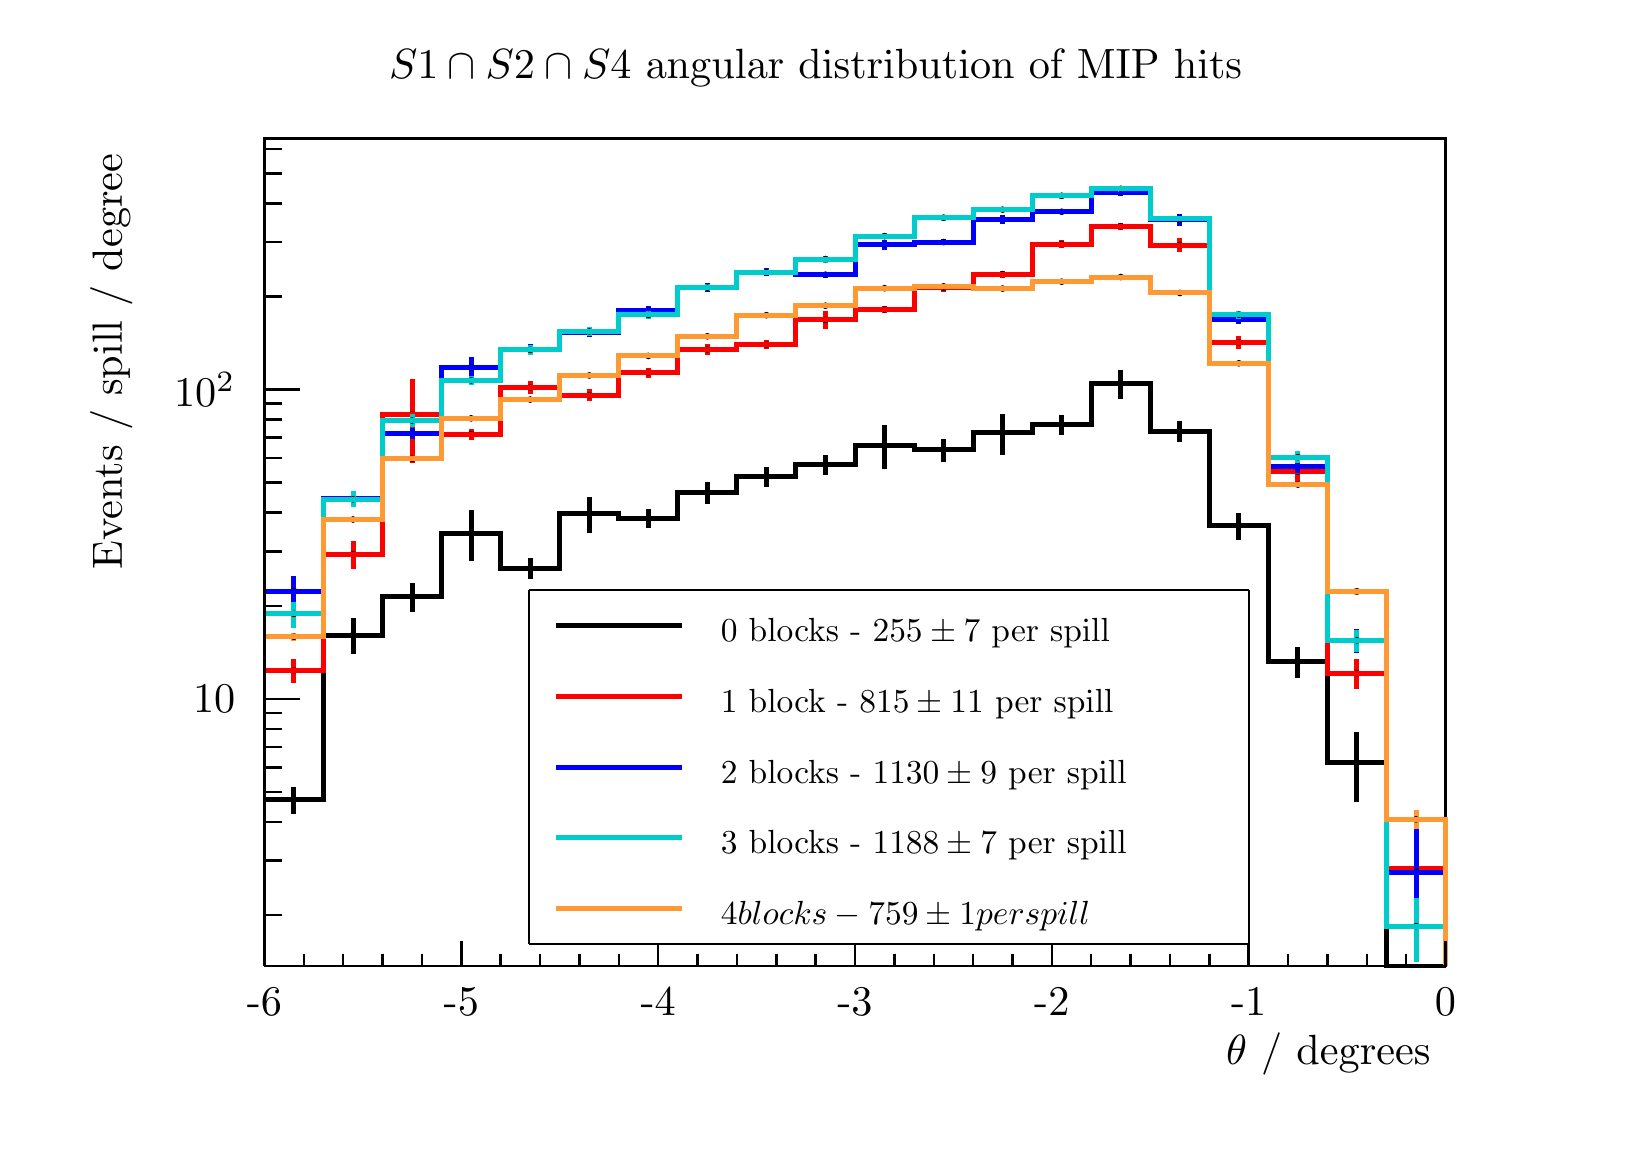
\begin{tikzpicture}
\pgfdeclareplotmark{cross} {
\pgfpathmoveto{\pgfpoint{-0.3\pgfplotmarksize}{\pgfplotmarksize}}
\pgfpathlineto{\pgfpoint{+0.3\pgfplotmarksize}{\pgfplotmarksize}}
\pgfpathlineto{\pgfpoint{+0.3\pgfplotmarksize}{0.3\pgfplotmarksize}}
\pgfpathlineto{\pgfpoint{+1\pgfplotmarksize}{0.3\pgfplotmarksize}}
\pgfpathlineto{\pgfpoint{+1\pgfplotmarksize}{-0.3\pgfplotmarksize}}
\pgfpathlineto{\pgfpoint{+0.3\pgfplotmarksize}{-0.3\pgfplotmarksize}}
\pgfpathlineto{\pgfpoint{+0.3\pgfplotmarksize}{-1.\pgfplotmarksize}}
\pgfpathlineto{\pgfpoint{-0.3\pgfplotmarksize}{-1.\pgfplotmarksize}}
\pgfpathlineto{\pgfpoint{-0.3\pgfplotmarksize}{-0.3\pgfplotmarksize}}
\pgfpathlineto{\pgfpoint{-1.\pgfplotmarksize}{-0.3\pgfplotmarksize}}
\pgfpathlineto{\pgfpoint{-1.\pgfplotmarksize}{0.3\pgfplotmarksize}}
\pgfpathlineto{\pgfpoint{-0.3\pgfplotmarksize}{0.3\pgfplotmarksize}}
\pgfpathclose
\pgfusepathqstroke
}
\pgfdeclareplotmark{cross*} {
\pgfpathmoveto{\pgfpoint{-0.3\pgfplotmarksize}{\pgfplotmarksize}}
\pgfpathlineto{\pgfpoint{+0.3\pgfplotmarksize}{\pgfplotmarksize}}
\pgfpathlineto{\pgfpoint{+0.3\pgfplotmarksize}{0.3\pgfplotmarksize}}
\pgfpathlineto{\pgfpoint{+1\pgfplotmarksize}{0.3\pgfplotmarksize}}
\pgfpathlineto{\pgfpoint{+1\pgfplotmarksize}{-0.3\pgfplotmarksize}}
\pgfpathlineto{\pgfpoint{+0.3\pgfplotmarksize}{-0.3\pgfplotmarksize}}
\pgfpathlineto{\pgfpoint{+0.3\pgfplotmarksize}{-1.\pgfplotmarksize}}
\pgfpathlineto{\pgfpoint{-0.3\pgfplotmarksize}{-1.\pgfplotmarksize}}
\pgfpathlineto{\pgfpoint{-0.3\pgfplotmarksize}{-0.3\pgfplotmarksize}}
\pgfpathlineto{\pgfpoint{-1.\pgfplotmarksize}{-0.3\pgfplotmarksize}}
\pgfpathlineto{\pgfpoint{-1.\pgfplotmarksize}{0.3\pgfplotmarksize}}
\pgfpathlineto{\pgfpoint{-0.3\pgfplotmarksize}{0.3\pgfplotmarksize}}
\pgfpathclose
\pgfusepathqfillstroke
}
\pgfdeclareplotmark{newstar} {
\pgfpathmoveto{\pgfqpoint{0pt}{\pgfplotmarksize}}
\pgfpathlineto{\pgfqpointpolar{44}{0.5\pgfplotmarksize}}
\pgfpathlineto{\pgfqpointpolar{18}{\pgfplotmarksize}}
\pgfpathlineto{\pgfqpointpolar{-20}{0.5\pgfplotmarksize}}
\pgfpathlineto{\pgfqpointpolar{-54}{\pgfplotmarksize}}
\pgfpathlineto{\pgfqpointpolar{-90}{0.5\pgfplotmarksize}}
\pgfpathlineto{\pgfqpointpolar{234}{\pgfplotmarksize}}
\pgfpathlineto{\pgfqpointpolar{198}{0.5\pgfplotmarksize}}
\pgfpathlineto{\pgfqpointpolar{162}{\pgfplotmarksize}}
\pgfpathlineto{\pgfqpointpolar{134}{0.5\pgfplotmarksize}}
\pgfpathclose
\pgfusepathqstroke
}
\pgfdeclareplotmark{newstar*} {
\pgfpathmoveto{\pgfqpoint{0pt}{\pgfplotmarksize}}
\pgfpathlineto{\pgfqpointpolar{44}{0.5\pgfplotmarksize}}
\pgfpathlineto{\pgfqpointpolar{18}{\pgfplotmarksize}}
\pgfpathlineto{\pgfqpointpolar{-20}{0.5\pgfplotmarksize}}
\pgfpathlineto{\pgfqpointpolar{-54}{\pgfplotmarksize}}
\pgfpathlineto{\pgfqpointpolar{-90}{0.5\pgfplotmarksize}}
\pgfpathlineto{\pgfqpointpolar{234}{\pgfplotmarksize}}
\pgfpathlineto{\pgfqpointpolar{198}{0.5\pgfplotmarksize}}
\pgfpathlineto{\pgfqpointpolar{162}{\pgfplotmarksize}}
\pgfpathlineto{\pgfqpointpolar{134}{0.5\pgfplotmarksize}}
\pgfpathclose
\pgfusepathqfillstroke
}
\definecolor{c}{rgb}{1,1,1};
\draw [color=c, fill=c] (0,0) rectangle (20,14.0115);
\draw [color=c, fill=c] (3,2.10172) rectangle (18,12.6103);
\definecolor{c}{rgb}{0,0,0};
\draw [c,line width=0.9] (3,2.10172) -- (3,12.6103) -- (18,12.6103) -- (18,2.10172) -- (3,2.10172);
\definecolor{c}{rgb}{1,1,1};
\draw [color=c, fill=c] (3,2.10172) rectangle (18,12.6103);
\definecolor{c}{rgb}{0,0,0};
\draw [c,line width=0.9] (3,2.10172) -- (3,12.6103) -- (18,12.6103) -- (18,2.10172) -- (3,2.10172);
\definecolor{c}{rgb}{0,0,0.6};
\draw [c,line width=0.9] (3,2.10172) -- (3.75,2.10172) -- (3.75,2.10172) -- (4.5,2.10172) -- (4.5,2.10172) -- (5.25,2.10172) -- (5.25,2.10172) -- (6,2.10172) -- (6,2.10172) -- (6.75,2.10172) -- (6.75,2.10172) -- (7.5,2.10172) -- (7.5,2.10172) --
 (8.25,2.10172) -- (8.25,2.10172) -- (9,2.10172) -- (9,2.10172) -- (9.75,2.10172) -- (9.75,2.10172) -- (10.5,2.10172) -- (10.5,2.10172) -- (11.25,2.10172) -- (11.25,2.10172) -- (12,2.10172) -- (12,2.10172) -- (12.75,2.10172) -- (12.75,2.10172) --
 (13.5,2.10172) -- (13.5,2.10172) -- (14.25,2.10172) -- (14.25,2.10172) -- (15,2.10172) -- (15,2.10172) -- (15.75,2.10172) -- (15.75,2.10172) -- (16.5,2.10172) -- (16.5,2.10172) -- (17.25,2.10172) -- (17.25,2.10172) -- (18,2.10172) -- (18,2.10172);
\definecolor{c}{rgb}{0,0,0};
\draw [c,line width=0.9] (3,2.10172) -- (18,2.10172);
\draw [c,line width=0.9] (3,2.41698) -- (3,2.10172);
\draw [c,line width=0.9] (3.5,2.25935) -- (3.5,2.10172);
\draw [c,line width=0.9] (4,2.25935) -- (4,2.10172);
\draw [c,line width=0.9] (4.5,2.25935) -- (4.5,2.10172);
\draw [c,line width=0.9] (5,2.25935) -- (5,2.10172);
\draw [c,line width=0.9] (5.5,2.41698) -- (5.5,2.10172);
\draw [c,line width=0.9] (6,2.25935) -- (6,2.10172);
\draw [c,line width=0.9] (6.5,2.25935) -- (6.5,2.10172);
\draw [c,line width=0.9] (7,2.25935) -- (7,2.10172);
\draw [c,line width=0.9] (7.5,2.25935) -- (7.5,2.10172);
\draw [c,line width=0.9] (8,2.41698) -- (8,2.10172);
\draw [c,line width=0.9] (8.5,2.25935) -- (8.5,2.10172);
\draw [c,line width=0.9] (9,2.25935) -- (9,2.10172);
\draw [c,line width=0.9] (9.5,2.25935) -- (9.5,2.10172);
\draw [c,line width=0.9] (10,2.25935) -- (10,2.10172);
\draw [c,line width=0.9] (10.5,2.41698) -- (10.5,2.10172);
\draw [c,line width=0.9] (11,2.25935) -- (11,2.10172);
\draw [c,line width=0.9] (11.5,2.25935) -- (11.5,2.10172);
\draw [c,line width=0.9] (12,2.25935) -- (12,2.10172);
\draw [c,line width=0.9] (12.5,2.25935) -- (12.5,2.10172);
\draw [c,line width=0.9] (13,2.41698) -- (13,2.10172);
\draw [c,line width=0.9] (13.5,2.25935) -- (13.5,2.10172);
\draw [c,line width=0.9] (14,2.25935) -- (14,2.10172);
\draw [c,line width=0.9] (14.5,2.25935) -- (14.5,2.10172);
\draw [c,line width=0.9] (15,2.25935) -- (15,2.10172);
\draw [c,line width=0.9] (15.5,2.41698) -- (15.5,2.10172);
\draw [c,line width=0.9] (16,2.25935) -- (16,2.10172);
\draw [c,line width=0.9] (16.5,2.25935) -- (16.5,2.10172);
\draw [c,line width=0.9] (17,2.25935) -- (17,2.10172);
\draw [c,line width=0.9] (17.5,2.25935) -- (17.5,2.10172);
\draw [c,line width=0.9] (18,2.41698) -- (18,2.10172);
\draw [anchor=base] (3,1.4712) node[scale=1.52731, color=c, rotate=0]{-6};
\draw [anchor=base] (5.5,1.4712) node[scale=1.52731, color=c, rotate=0]{-5};
\draw [anchor=base] (8,1.4712) node[scale=1.52731, color=c, rotate=0]{-4};
\draw [anchor=base] (10.5,1.4712) node[scale=1.52731, color=c, rotate=0]{-3};
\draw [anchor=base] (13,1.4712) node[scale=1.52731, color=c, rotate=0]{-2};
\draw [anchor=base] (15.5,1.4712) node[scale=1.52731, color=c, rotate=0]{-1};
\draw [anchor=base] (18,1.4712) node[scale=1.52731, color=c, rotate=0]{0};
\draw [anchor= east] (18,0.980802) node[scale=1.52731, color=c, rotate=0]{$\theta$ / degrees};
\draw [c,line width=0.9] (3,2.10172) -- (3,12.6103);
\draw [c,line width=0.9] (3.225,2.74878) -- (3,2.74878);
\draw [c,line width=0.9] (3.225,3.44048) -- (3,3.44048);
\draw [c,line width=0.9] (3.225,3.93125) -- (3,3.93125);
\draw [c,line width=0.9] (3.225,4.31191) -- (3,4.31191);
\draw [c,line width=0.9] (3.225,4.62294) -- (3,4.62294);
\draw [c,line width=0.9] (3.225,4.88591) -- (3,4.88591);
\draw [c,line width=0.9] (3.225,5.11371) -- (3,5.11371);
\draw [c,line width=0.9] (3.225,5.31464) -- (3,5.31464);
\draw [c,line width=0.9] (3.45,5.49438) -- (3,5.49438);
\draw [anchor= east] (2.82,5.49438) node[scale=1.52731, color=c, rotate=0]{10};
\draw [c,line width=0.9] (3.225,6.67684) -- (3,6.67684);
\draw [c,line width=0.9] (3.225,7.36854) -- (3,7.36854);
\draw [c,line width=0.9] (3.225,7.85931) -- (3,7.85931);
\draw [c,line width=0.9] (3.225,8.23998) -- (3,8.23998);
\draw [c,line width=0.9] (3.225,8.55101) -- (3,8.55101);
\draw [c,line width=0.9] (3.225,8.81398) -- (3,8.81398);
\draw [c,line width=0.9] (3.225,9.04177) -- (3,9.04177);
\draw [c,line width=0.9] (3.225,9.2427) -- (3,9.2427);
\draw [c,line width=0.9] (3.45,9.42244) -- (3,9.42244);
\draw [anchor= east] (2.82,9.42244) node[scale=1.52731, color=c, rotate=0]{$10^{2}$};
\draw [c,line width=0.9] (3.225,10.6049) -- (3,10.6049);
\draw [c,line width=0.9] (3.225,11.2966) -- (3,11.2966);
\draw [c,line width=0.9] (3.225,11.7874) -- (3,11.7874);
\draw [c,line width=0.9] (3.225,12.168) -- (3,12.168);
\draw [c,line width=0.9] (3.225,12.4791) -- (3,12.4791);
\draw [anchor= east] (1.05444,12.6103) node[scale=1.52731, color=c, rotate=90]{ Events / spill / degree};
\draw [c,line width=1.8] (3.375,4.03479) -- (3.375,4.21511);
\draw [c,line width=1.8] (3.375,4.21511) -- (3.375,4.37817);
\foreach \P in {(3.375,4.21511)}{\draw[mark options={color=c,fill=c},mark size=2.402402pt,mark=*,mark size=1pt] plot coordinates {\P};}
\draw [c,line width=1.8] (4.125,6.06456) -- (4.125,6.30527);
\draw [c,line width=1.8] (4.125,6.30527) -- (4.125,6.51617);
\foreach \P in {(4.125,6.30527)}{\draw[mark options={color=c,fill=c},mark size=2.402402pt,mark=*,mark size=1pt] plot coordinates {\P};}
\draw [c,line width=1.8] (4.875,6.59289) -- (4.875,6.79255);
\draw [c,line width=1.8] (4.875,6.79255) -- (4.875,6.97128);
\foreach \P in {(4.875,6.79255)}{\draw[mark options={color=c,fill=c},mark size=2.402402pt,mark=*,mark size=1pt] plot coordinates {\P};}
\draw [c,line width=1.8] (5.625,7.24345) -- (5.625,7.59827);
\draw [c,line width=1.8] (5.625,7.59827) -- (5.625,7.89184);
\foreach \P in {(5.625,7.59827)}{\draw[mark options={color=c,fill=c},mark size=2.402402pt,mark=*,mark size=1pt] plot coordinates {\P};}
\draw [c,line width=1.8] (6.375,7.0209) -- (6.375,7.15415);
\draw [c,line width=1.8] (6.375,7.15415) -- (6.375,7.27775);
\foreach \P in {(6.375,7.15415)}{\draw[mark options={color=c,fill=c},mark size=2.402402pt,mark=*,mark size=1pt] plot coordinates {\P};}
\draw [c,line width=1.8] (7.125,7.59869) -- (7.125,7.84484);
\draw [c,line width=1.8] (7.125,7.84484) -- (7.125,8.05991);
\foreach \P in {(7.125,7.84484)}{\draw[mark options={color=c,fill=c},mark size=2.402402pt,mark=*,mark size=1pt] plot coordinates {\P};}
\draw [c,line width=1.8] (7.875,7.66128) -- (7.875,7.78909);
\draw [c,line width=1.8] (7.875,7.78909) -- (7.875,7.90799);
\foreach \P in {(7.875,7.78909)}{\draw[mark options={color=c,fill=c},mark size=2.402402pt,mark=*,mark size=1pt] plot coordinates {\P};}
\draw [c,line width=1.8] (8.625,7.96983) -- (8.625,8.11244);
\draw [c,line width=1.8] (8.625,8.11244) -- (8.625,8.24405);
\foreach \P in {(8.625,8.11244)}{\draw[mark options={color=c,fill=c},mark size=2.402402pt,mark=*,mark size=1pt] plot coordinates {\P};}
\draw [c,line width=1.8] (9.375,8.17892) -- (9.375,8.31357);
\draw [c,line width=1.8] (9.375,8.31357) -- (9.375,8.43837);
\foreach \P in {(9.375,8.31357)}{\draw[mark options={color=c,fill=c},mark size=2.402402pt,mark=*,mark size=1pt] plot coordinates {\P};}
\draw [c,line width=1.8] (10.125,8.33421) -- (10.125,8.46593);
\draw [c,line width=1.8] (10.125,8.46593) -- (10.125,8.58821);
\foreach \P in {(10.125,8.46593)}{\draw[mark options={color=c,fill=c},mark size=2.402402pt,mark=*,mark size=1pt] plot coordinates {\P};}
\draw [c,line width=1.8] (10.875,8.40736) -- (10.875,8.71387);
\draw [c,line width=1.8] (10.875,8.71387) -- (10.875,8.9736);
\foreach \P in {(10.875,8.71387)}{\draw[mark options={color=c,fill=c},mark size=2.402402pt,mark=*,mark size=1pt] plot coordinates {\P};}
\draw [c,line width=1.8] (11.625,8.50247) -- (11.625,8.65545);
\draw [c,line width=1.8] (11.625,8.65545) -- (11.625,8.79583);
\foreach \P in {(11.625,8.65545)}{\draw[mark options={color=c,fill=c},mark size=2.402402pt,mark=*,mark size=1pt] plot coordinates {\P};}
\draw [c,line width=1.8] (12.375,8.59757) -- (12.375,8.87469);
\draw [c,line width=1.8] (12.375,8.87469) -- (12.375,9.11301);
\foreach \P in {(12.375,8.87469)}{\draw[mark options={color=c,fill=c},mark size=2.402402pt,mark=*,mark size=1pt] plot coordinates {\P};}
\draw [c,line width=1.8] (13.125,8.84578) -- (13.125,8.97996);
\draw [c,line width=1.8] (13.125,8.97996) -- (13.125,9.10434);
\foreach \P in {(13.125,8.97996)}{\draw[mark options={color=c,fill=c},mark size=2.402402pt,mark=*,mark size=1pt] plot coordinates {\P};}
\draw [c,line width=1.8] (13.875,9.30442) -- (13.875,9.49928);
\draw [c,line width=1.8] (13.875,9.49928) -- (13.875,9.67416);
\foreach \P in {(13.875,9.49928)}{\draw[mark options={color=c,fill=c},mark size=2.402402pt,mark=*,mark size=1pt] plot coordinates {\P};}
\draw [c,line width=1.8] (14.625,8.75179) -- (14.625,8.89211);
\draw [c,line width=1.8] (14.625,8.89211) -- (14.625,9.02176);
\foreach \P in {(14.625,8.89211)}{\draw[mark options={color=c,fill=c},mark size=2.402402pt,mark=*,mark size=1pt] plot coordinates {\P};}
\draw [c,line width=1.8] (15.375,7.50871) -- (15.375,7.69028);
\draw [c,line width=1.8] (15.375,7.69028) -- (15.375,7.85438);
\foreach \P in {(15.375,7.69028)}{\draw[mark options={color=c,fill=c},mark size=2.402402pt,mark=*,mark size=1pt] plot coordinates {\P};}
\draw [c,line width=1.8] (16.125,5.75699) -- (16.125,5.96327);
\draw [c,line width=1.8] (16.125,5.96327) -- (16.125,6.14727);
\foreach \P in {(16.125,5.96327)}{\draw[mark options={color=c,fill=c},mark size=2.402402pt,mark=*,mark size=1pt] plot coordinates {\P};}
\draw [c,line width=1.8] (16.875,4.1801) -- (16.875,4.6868);
\draw [c,line width=1.8] (16.875,4.6868) -- (16.875,5.07696);
\foreach \P in {(16.875,4.6868)}{\draw[mark options={color=c,fill=c},mark size=2.402402pt,mark=*,mark size=1pt] plot coordinates {\P};}
\draw [c,line width=1.8] (3,4.21511) -- (3.75,4.21511) -- (3.75,6.30527) -- (4.5,6.30527) -- (4.5,6.79255) -- (5.25,6.79255) -- (5.25,7.59827) -- (6,7.59827) -- (6,7.15415) -- (6.75,7.15415) -- (6.75,7.84484) -- (7.5,7.84484) -- (7.5,7.78909) --
 (8.25,7.78909) -- (8.25,8.11244) -- (9,8.11244) -- (9,8.31357) -- (9.75,8.31357) -- (9.75,8.46593) -- (10.5,8.46593) -- (10.5,8.71387) -- (11.25,8.71387) -- (11.25,8.65545) -- (12,8.65545) -- (12,8.87469) -- (12.75,8.87469) -- (12.75,8.97996) --
 (13.5,8.97996) -- (13.5,9.49928) -- (14.25,9.49928) -- (14.25,8.89211) -- (15,8.89211) -- (15,7.69028) -- (15.75,7.69028) -- (15.75,5.96327) -- (16.5,5.96327) -- (16.5,4.6868) -- (17.25,4.6868) -- (17.25,2.10172) -- (18,2.10172) -- (18,2.10172);
\definecolor{c}{rgb}{1,0,0};
\draw [c,line width=1.8] (3.375,5.69435) -- (3.375,5.85486);
\draw [c,line width=1.8] (3.375,5.85486) -- (3.375,6.00157);
\definecolor{c}{rgb}{0,0,0};
\foreach \P in {(3.375,5.85486)}{\draw[mark options={color=c,fill=c},mark size=2.402402pt,mark=*,mark size=1pt] plot coordinates {\P};}
\definecolor{c}{rgb}{1,0,0};
\draw [c,line width=1.8] (4.125,7.13733) -- (4.125,7.33122);
\draw [c,line width=1.8] (4.125,7.33122) -- (4.125,7.50531);
\definecolor{c}{rgb}{0,0,0};
\foreach \P in {(4.125,7.33122)}{\draw[mark options={color=c,fill=c},mark size=2.402402pt,mark=*,mark size=1pt] plot coordinates {\P};}
\definecolor{c}{rgb}{1,0,0};
\draw [c,line width=1.8] (4.875,8.49291) -- (4.875,9.10662);
\draw [c,line width=1.8] (4.875,9.10662) -- (4.875,9.55702);
\definecolor{c}{rgb}{0,0,0};
\foreach \P in {(4.875,9.10662)}{\draw[mark options={color=c,fill=c},mark size=2.402402pt,mark=*,mark size=1pt] plot coordinates {\P};}
\definecolor{c}{rgb}{1,0,0};
\draw [c,line width=1.8] (5.625,8.78671) -- (5.625,8.85696);
\draw [c,line width=1.8] (5.625,8.85696) -- (5.625,8.92444);
\definecolor{c}{rgb}{0,0,0};
\foreach \P in {(5.625,8.85696)}{\draw[mark options={color=c,fill=c},mark size=2.402402pt,mark=*,mark size=1pt] plot coordinates {\P};}
\definecolor{c}{rgb}{1,0,0};
\draw [c,line width=1.8] (6.375,9.36058) -- (6.375,9.44798);
\draw [c,line width=1.8] (6.375,9.44798) -- (6.375,9.53112);
\definecolor{c}{rgb}{0,0,0};
\foreach \P in {(6.375,9.44798)}{\draw[mark options={color=c,fill=c},mark size=2.402402pt,mark=*,mark size=1pt] plot coordinates {\P};}
\definecolor{c}{rgb}{1,0,0};
\draw [c,line width=1.8] (7.125,9.27103) -- (7.125,9.34886);
\draw [c,line width=1.8] (7.125,9.34886) -- (7.125,9.4233);
\definecolor{c}{rgb}{0,0,0};
\foreach \P in {(7.125,9.34886)}{\draw[mark options={color=c,fill=c},mark size=2.402402pt,mark=*,mark size=1pt] plot coordinates {\P};}
\definecolor{c}{rgb}{1,0,0};
\draw [c,line width=1.8] (7.875,9.57391) -- (7.875,9.6376);
\draw [c,line width=1.8] (7.875,9.6376) -- (7.875,9.69901);
\definecolor{c}{rgb}{0,0,0};
\foreach \P in {(7.875,9.6376)}{\draw[mark options={color=c,fill=c},mark size=2.402402pt,mark=*,mark size=1pt] plot coordinates {\P};}
\definecolor{c}{rgb}{1,0,0};
\draw [c,line width=1.8] (8.625,9.86531) -- (8.625,9.93131);
\draw [c,line width=1.8] (8.625,9.93131) -- (8.625,9.99484);
\definecolor{c}{rgb}{0,0,0};
\foreach \P in {(8.625,9.93131)}{\draw[mark options={color=c,fill=c},mark size=2.402402pt,mark=*,mark size=1pt] plot coordinates {\P};}
\definecolor{c}{rgb}{1,0,0};
\draw [c,line width=1.8] (9.375,9.93416) -- (9.375,9.99291);
\draw [c,line width=1.8] (9.375,9.99291) -- (9.375,10.0497);
\definecolor{c}{rgb}{0,0,0};
\foreach \P in {(9.375,9.99291)}{\draw[mark options={color=c,fill=c},mark size=2.402402pt,mark=*,mark size=1pt] plot coordinates {\P};}
\definecolor{c}{rgb}{1,0,0};
\draw [c,line width=1.8] (10.125,10.1876) -- (10.125,10.3081);
\draw [c,line width=1.8] (10.125,10.3081) -- (10.125,10.4207);
\definecolor{c}{rgb}{0,0,0};
\foreach \P in {(10.125,10.3081)}{\draw[mark options={color=c,fill=c},mark size=2.402402pt,mark=*,mark size=1pt] plot coordinates {\P};}
\definecolor{c}{rgb}{1,0,0};
\draw [c,line width=1.8] (10.875,10.3908) -- (10.875,10.4405);
\draw [c,line width=1.8] (10.875,10.4405) -- (10.875,10.4888);
\definecolor{c}{rgb}{0,0,0};
\foreach \P in {(10.875,10.4405)}{\draw[mark options={color=c,fill=c},mark size=2.402402pt,mark=*,mark size=1pt] plot coordinates {\P};}
\definecolor{c}{rgb}{1,0,0};
\draw [c,line width=1.8] (11.625,10.6611) -- (11.625,10.7143);
\draw [c,line width=1.8] (11.625,10.7143) -- (11.625,10.7659);
\definecolor{c}{rgb}{0,0,0};
\foreach \P in {(11.625,10.7143)}{\draw[mark options={color=c,fill=c},mark size=2.402402pt,mark=*,mark size=1pt] plot coordinates {\P};}
\definecolor{c}{rgb}{1,0,0};
\draw [c,line width=1.8] (12.375,10.842) -- (12.375,10.8886);
\draw [c,line width=1.8] (12.375,10.8886) -- (12.375,10.934);
\definecolor{c}{rgb}{0,0,0};
\foreach \P in {(12.375,10.8886)}{\draw[mark options={color=c,fill=c},mark size=2.402402pt,mark=*,mark size=1pt] plot coordinates {\P};}
\definecolor{c}{rgb}{1,0,0};
\draw [c,line width=1.8] (13.125,11.2205) -- (13.125,11.2707);
\draw [c,line width=1.8] (13.125,11.2707) -- (13.125,11.3196);
\definecolor{c}{rgb}{0,0,0};
\foreach \P in {(13.125,11.2707)}{\draw[mark options={color=c,fill=c},mark size=2.402402pt,mark=*,mark size=1pt] plot coordinates {\P};}
\definecolor{c}{rgb}{1,0,0};
\draw [c,line width=1.8] (13.875,11.4485) -- (13.875,11.4966);
\draw [c,line width=1.8] (13.875,11.4966) -- (13.875,11.5434);
\definecolor{c}{rgb}{0,0,0};
\foreach \P in {(13.875,11.4966)}{\draw[mark options={color=c,fill=c},mark size=2.402402pt,mark=*,mark size=1pt] plot coordinates {\P};}
\definecolor{c}{rgb}{1,0,0};
\draw [c,line width=1.8] (14.625,11.1707) -- (14.625,11.258);
\draw [c,line width=1.8] (14.625,11.258) -- (14.625,11.3411);
\definecolor{c}{rgb}{0,0,0};
\foreach \P in {(14.625,11.258)}{\draw[mark options={color=c,fill=c},mark size=2.402402pt,mark=*,mark size=1pt] plot coordinates {\P};}
\definecolor{c}{rgb}{1,0,0};
\draw [c,line width=1.8] (15.375,9.94073) -- (15.375,10.0212);
\draw [c,line width=1.8] (15.375,10.0212) -- (15.375,10.098);
\definecolor{c}{rgb}{0,0,0};
\foreach \P in {(15.375,10.0212)}{\draw[mark options={color=c,fill=c},mark size=2.402402pt,mark=*,mark size=1pt] plot coordinates {\P};}
\definecolor{c}{rgb}{1,0,0};
\draw [c,line width=1.8] (16.125,8.20348) -- (16.125,8.37878);
\draw [c,line width=1.8] (16.125,8.37878) -- (16.125,8.53773);
\definecolor{c}{rgb}{0,0,0};
\foreach \P in {(16.125,8.37878)}{\draw[mark options={color=c,fill=c},mark size=2.402402pt,mark=*,mark size=1pt] plot coordinates {\P};}
\definecolor{c}{rgb}{1,0,0};
\draw [c,line width=1.8] (16.875,5.61778) -- (16.875,5.81947);
\draw [c,line width=1.8] (16.875,5.81947) -- (16.875,5.99982);
\definecolor{c}{rgb}{0,0,0};
\foreach \P in {(16.875,5.81947)}{\draw[mark options={color=c,fill=c},mark size=2.402402pt,mark=*,mark size=1pt] plot coordinates {\P};}
\definecolor{c}{rgb}{1,0,0};
\draw [c,line width=1.8] (17.625,2.81258) -- (17.625,3.33608);
\draw [c,line width=1.8] (17.625,3.33608) -- (17.625,3.7361);
\definecolor{c}{rgb}{0,0,0};
\foreach \P in {(17.625,3.33608)}{\draw[mark options={color=c,fill=c},mark size=2.402402pt,mark=*,mark size=1pt] plot coordinates {\P};}
\definecolor{c}{rgb}{1,0,0};
\draw [c,line width=1.8] (3,5.85486) -- (3.75,5.85486) -- (3.75,7.33122) -- (4.5,7.33122) -- (4.5,9.10662) -- (5.25,9.10662) -- (5.25,8.85696) -- (6,8.85696) -- (6,9.44798) -- (6.75,9.44798) -- (6.75,9.34886) -- (7.5,9.34886) -- (7.5,9.6376) --
 (8.25,9.6376) -- (8.25,9.93131) -- (9,9.93131) -- (9,9.99291) -- (9.75,9.99291) -- (9.75,10.3081) -- (10.5,10.3081) -- (10.5,10.4405) -- (11.25,10.4405) -- (11.25,10.7143) -- (12,10.7143) -- (12,10.8886) -- (12.75,10.8886) -- (12.75,11.2707) --
 (13.5,11.2707) -- (13.5,11.4966) -- (14.25,11.4966) -- (14.25,11.258) -- (15,11.258) -- (15,10.0212) -- (15.75,10.0212) -- (15.75,8.37878) -- (16.5,8.37878) -- (16.5,5.81947) -- (17.25,5.81947) -- (17.25,3.33608) -- (18,3.33608) -- (18,2.10172);
\definecolor{c}{rgb}{0,0,1};
\draw [c,line width=1.8] (3.375,6.65616) -- (3.375,6.8638);
\draw [c,line width=1.8] (3.375,6.8638) -- (3.375,7.04889);
\definecolor{c}{rgb}{0,0,0};
\foreach \P in {(3.375,6.8638)}{\draw[mark options={color=c,fill=c},mark size=2.402402pt,mark=*,mark size=1pt] plot coordinates {\P};}
\definecolor{c}{rgb}{0,0,1};
\draw [c,line width=1.8] (4.125,7.95275) -- (4.125,8.03964);
\draw [c,line width=1.8] (4.125,8.03964) -- (4.125,8.12233);
\definecolor{c}{rgb}{0,0,0};
\foreach \P in {(4.125,8.03964)}{\draw[mark options={color=c,fill=c},mark size=2.402402pt,mark=*,mark size=1pt] plot coordinates {\P};}
\definecolor{c}{rgb}{0,0,1};
\draw [c,line width=1.8] (4.875,8.79676) -- (4.875,8.86516);
\draw [c,line width=1.8] (4.875,8.86516) -- (4.875,8.93093);
\definecolor{c}{rgb}{0,0,0};
\foreach \P in {(4.875,8.86516)}{\draw[mark options={color=c,fill=c},mark size=2.402402pt,mark=*,mark size=1pt] plot coordinates {\P};}
\definecolor{c}{rgb}{0,0,1};
\draw [c,line width=1.8] (5.625,9.56311) -- (5.625,9.70472);
\draw [c,line width=1.8] (5.625,9.70472) -- (5.625,9.83546);
\definecolor{c}{rgb}{0,0,0};
\foreach \P in {(5.625,9.70472)}{\draw[mark options={color=c,fill=c},mark size=2.402402pt,mark=*,mark size=1pt] plot coordinates {\P};}
\definecolor{c}{rgb}{0,0,1};
\draw [c,line width=1.8] (6.375,9.86868) -- (6.375,9.93349);
\draw [c,line width=1.8] (6.375,9.93349) -- (6.375,9.99594);
\definecolor{c}{rgb}{0,0,0};
\foreach \P in {(6.375,9.93349)}{\draw[mark options={color=c,fill=c},mark size=2.402402pt,mark=*,mark size=1pt] plot coordinates {\P};}
\definecolor{c}{rgb}{0,0,1};
\draw [c,line width=1.8] (7.125,10.0923) -- (7.125,10.1467);
\draw [c,line width=1.8] (7.125,10.1467) -- (7.125,10.1994);
\definecolor{c}{rgb}{0,0,0};
\foreach \P in {(7.125,10.1467)}{\draw[mark options={color=c,fill=c},mark size=2.402402pt,mark=*,mark size=1pt] plot coordinates {\P};}
\definecolor{c}{rgb}{0,0,1};
\draw [c,line width=1.8] (7.875,10.3723) -- (7.875,10.4285);
\draw [c,line width=1.8] (7.875,10.4285) -- (7.875,10.483);
\definecolor{c}{rgb}{0,0,0};
\foreach \P in {(7.875,10.4285)}{\draw[mark options={color=c,fill=c},mark size=2.402402pt,mark=*,mark size=1pt] plot coordinates {\P};}
\definecolor{c}{rgb}{0,0,1};
\draw [c,line width=1.8] (8.625,10.6569) -- (8.625,10.7171);
\draw [c,line width=1.8] (8.625,10.7171) -- (8.625,10.7754);
\definecolor{c}{rgb}{0,0,0};
\foreach \P in {(8.625,10.7171)}{\draw[mark options={color=c,fill=c},mark size=2.402402pt,mark=*,mark size=1pt] plot coordinates {\P};}
\definecolor{c}{rgb}{0,0,1};
\draw [c,line width=1.8] (9.375,10.8604) -- (9.375,10.9138);
\draw [c,line width=1.8] (9.375,10.9138) -- (9.375,10.9655);
\definecolor{c}{rgb}{0,0,0};
\foreach \P in {(9.375,10.9138)}{\draw[mark options={color=c,fill=c},mark size=2.402402pt,mark=*,mark size=1pt] plot coordinates {\P};}
\definecolor{c}{rgb}{0,0,1};
\draw [c,line width=1.8] (10.125,10.8426) -- (10.125,10.8814);
\draw [c,line width=1.8] (10.125,10.8814) -- (10.125,10.9193);
\definecolor{c}{rgb}{0,0,0};
\foreach \P in {(10.125,10.8814)}{\draw[mark options={color=c,fill=c},mark size=2.402402pt,mark=*,mark size=1pt] plot coordinates {\P};}
\definecolor{c}{rgb}{0,0,1};
\draw [c,line width=1.8] (10.875,11.197) -- (10.875,11.2635);
\draw [c,line width=1.8] (10.875,11.2635) -- (10.875,11.3274);
\definecolor{c}{rgb}{0,0,0};
\foreach \P in {(10.875,11.2635)}{\draw[mark options={color=c,fill=c},mark size=2.402402pt,mark=*,mark size=1pt] plot coordinates {\P};}
\definecolor{c}{rgb}{0,0,1};
\draw [c,line width=1.8] (11.625,11.2611) -- (11.625,11.2957);
\draw [c,line width=1.8] (11.625,11.2957) -- (11.625,11.3296);
\definecolor{c}{rgb}{0,0,0};
\foreach \P in {(11.625,11.2957)}{\draw[mark options={color=c,fill=c},mark size=2.402402pt,mark=*,mark size=1pt] plot coordinates {\P};}
\definecolor{c}{rgb}{0,0,1};
\draw [c,line width=1.8] (12.375,11.5281) -- (12.375,11.5817);
\draw [c,line width=1.8] (12.375,11.5817) -- (12.375,11.6336);
\definecolor{c}{rgb}{0,0,0};
\foreach \P in {(12.375,11.5817)}{\draw[mark options={color=c,fill=c},mark size=2.402402pt,mark=*,mark size=1pt] plot coordinates {\P};}
\definecolor{c}{rgb}{0,0,1};
\draw [c,line width=1.8] (13.125,11.65) -- (13.125,11.6807);
\draw [c,line width=1.8] (13.125,11.6807) -- (13.125,11.7108);
\definecolor{c}{rgb}{0,0,0};
\foreach \P in {(13.125,11.6807)}{\draw[mark options={color=c,fill=c},mark size=2.402402pt,mark=*,mark size=1pt] plot coordinates {\P};}
\definecolor{c}{rgb}{0,0,1};
\draw [c,line width=1.8] (13.875,11.8858) -- (13.875,11.9233);
\draw [c,line width=1.8] (13.875,11.9233) -- (13.875,11.96);
\definecolor{c}{rgb}{0,0,0};
\foreach \P in {(13.875,11.9233)}{\draw[mark options={color=c,fill=c},mark size=2.402402pt,mark=*,mark size=1pt] plot coordinates {\P};}
\definecolor{c}{rgb}{0,0,1};
\draw [c,line width=1.8] (14.625,11.5052) -- (14.625,11.5773);
\draw [c,line width=1.8] (14.625,11.5773) -- (14.625,11.6465);
\definecolor{c}{rgb}{0,0,0};
\foreach \P in {(14.625,11.5773)}{\draw[mark options={color=c,fill=c},mark size=2.402402pt,mark=*,mark size=1pt] plot coordinates {\P};}
\definecolor{c}{rgb}{0,0,1};
\draw [c,line width=1.8] (15.375,10.2584) -- (15.375,10.3138);
\draw [c,line width=1.8] (15.375,10.3138) -- (15.375,10.3674);
\definecolor{c}{rgb}{0,0,0};
\foreach \P in {(15.375,10.3138)}{\draw[mark options={color=c,fill=c},mark size=2.402402pt,mark=*,mark size=1pt] plot coordinates {\P};}
\definecolor{c}{rgb}{0,0,1};
\draw [c,line width=1.8] (16.125,8.36025) -- (16.125,8.4466);
\draw [c,line width=1.8] (16.125,8.4466) -- (16.125,8.52878);
\definecolor{c}{rgb}{0,0,0};
\foreach \P in {(16.125,8.4466)}{\draw[mark options={color=c,fill=c},mark size=2.402402pt,mark=*,mark size=1pt] plot coordinates {\P};}
\definecolor{c}{rgb}{0,0,1};
\draw [c,line width=1.8] (16.875,6.08301) -- (16.875,6.24076);
\draw [c,line width=1.8] (16.875,6.24076) -- (16.875,6.38515);
\definecolor{c}{rgb}{0,0,0};
\foreach \P in {(16.875,6.24076)}{\draw[mark options={color=c,fill=c},mark size=2.402402pt,mark=*,mark size=1pt] plot coordinates {\P};}
\definecolor{c}{rgb}{0,0,1};
\draw [c,line width=1.8] (17.625,2.24304) -- (17.625,3.29519);
\draw [c,line width=1.8] (17.625,3.29519) -- (17.625,3.94114);
\definecolor{c}{rgb}{0,0,0};
\foreach \P in {(17.625,3.29519)}{\draw[mark options={color=c,fill=c},mark size=2.402402pt,mark=*,mark size=1pt] plot coordinates {\P};}
\definecolor{c}{rgb}{0,0,1};
\draw [c,line width=1.8] (3,6.8638) -- (3.75,6.8638) -- (3.75,8.03964) -- (4.5,8.03964) -- (4.5,8.86516) -- (5.25,8.86516) -- (5.25,9.70472) -- (6,9.70472) -- (6,9.93349) -- (6.75,9.93349) -- (6.75,10.1467) -- (7.5,10.1467) -- (7.5,10.4285) --
 (8.25,10.4285) -- (8.25,10.7171) -- (9,10.7171) -- (9,10.9138) -- (9.75,10.9138) -- (9.75,10.8814) -- (10.5,10.8814) -- (10.5,11.2635) -- (11.25,11.2635) -- (11.25,11.2957) -- (12,11.2957) -- (12,11.5817) -- (12.75,11.5817) -- (12.75,11.6807) --
 (13.5,11.6807) -- (13.5,11.9233) -- (14.25,11.9233) -- (14.25,11.5773) -- (15,11.5773) -- (15,10.3138) -- (15.75,10.3138) -- (15.75,8.4466) -- (16.5,8.4466) -- (16.5,6.24076) -- (17.25,6.24076) -- (17.25,3.29519) -- (18,3.29519) -- (18,2.10172);
\definecolor{c}{rgb}{0,0.8,0.8};
\draw [c,line width=1.8] (3.375,6.40051) -- (3.375,6.57328);
\draw [c,line width=1.8] (3.375,6.57328) -- (3.375,6.73014);
\definecolor{c}{rgb}{0,0,0};
\foreach \P in {(3.375,6.57328)}{\draw[mark options={color=c,fill=c},mark size=2.402402pt,mark=*,mark size=1pt] plot coordinates {\P};}
\definecolor{c}{rgb}{0,0.8,0.8};
\draw [c,line width=1.8] (4.125,7.9248) -- (4.125,8.02937);
\draw [c,line width=1.8] (4.125,8.02937) -- (4.125,8.12789);
\definecolor{c}{rgb}{0,0,0};
\foreach \P in {(4.125,8.02937)}{\draw[mark options={color=c,fill=c},mark size=2.402402pt,mark=*,mark size=1pt] plot coordinates {\P};}
\definecolor{c}{rgb}{0,0.8,0.8};
\draw [c,line width=1.8] (4.875,8.94752) -- (4.875,9.02906);
\draw [c,line width=1.8] (4.875,9.02906) -- (4.875,9.10688);
\definecolor{c}{rgb}{0,0,0};
\foreach \P in {(4.875,9.02906)}{\draw[mark options={color=c,fill=c},mark size=2.402402pt,mark=*,mark size=1pt] plot coordinates {\P};}
\definecolor{c}{rgb}{0,0.8,0.8};
\draw [c,line width=1.8] (5.625,9.4765) -- (5.625,9.53891);
\draw [c,line width=1.8] (5.625,9.53891) -- (5.625,9.59913);
\definecolor{c}{rgb}{0,0,0};
\foreach \P in {(5.625,9.53891)}{\draw[mark options={color=c,fill=c},mark size=2.402402pt,mark=*,mark size=1pt] plot coordinates {\P};}
\definecolor{c}{rgb}{0,0.8,0.8};
\draw [c,line width=1.8] (6.375,9.86024) -- (6.375,9.92617);
\draw [c,line width=1.8] (6.375,9.92617) -- (6.375,9.98965);
\definecolor{c}{rgb}{0,0,0};
\foreach \P in {(6.375,9.92617)}{\draw[mark options={color=c,fill=c},mark size=2.402402pt,mark=*,mark size=1pt] plot coordinates {\P};}
\definecolor{c}{rgb}{0,0.8,0.8};
\draw [c,line width=1.8] (7.125,10.1072) -- (7.125,10.1601);
\draw [c,line width=1.8] (7.125,10.1601) -- (7.125,10.2114);
\definecolor{c}{rgb}{0,0,0};
\foreach \P in {(7.125,10.1601)}{\draw[mark options={color=c,fill=c},mark size=2.402402pt,mark=*,mark size=1pt] plot coordinates {\P};}
\definecolor{c}{rgb}{0,0.8,0.8};
\draw [c,line width=1.8] (7.875,10.3237) -- (7.875,10.3698);
\draw [c,line width=1.8] (7.875,10.3698) -- (7.875,10.4147);
\definecolor{c}{rgb}{0,0,0};
\foreach \P in {(7.875,10.3698)}{\draw[mark options={color=c,fill=c},mark size=2.402402pt,mark=*,mark size=1pt] plot coordinates {\P};}
\definecolor{c}{rgb}{0,0.8,0.8};
\draw [c,line width=1.8] (8.625,10.6703) -- (8.625,10.7158);
\draw [c,line width=1.8] (8.625,10.7158) -- (8.625,10.7602);
\definecolor{c}{rgb}{0,0,0};
\foreach \P in {(8.625,10.7158)}{\draw[mark options={color=c,fill=c},mark size=2.402402pt,mark=*,mark size=1pt] plot coordinates {\P};}
\definecolor{c}{rgb}{0,0.8,0.8};
\draw [c,line width=1.8] (9.375,10.8724) -- (9.375,10.9138);
\draw [c,line width=1.8] (9.375,10.9138) -- (9.375,10.9541);
\definecolor{c}{rgb}{0,0,0};
\foreach \P in {(9.375,10.9138)}{\draw[mark options={color=c,fill=c},mark size=2.402402pt,mark=*,mark size=1pt] plot coordinates {\P};}
\definecolor{c}{rgb}{0,0.8,0.8};
\draw [c,line width=1.8] (10.125,11.0354) -- (10.125,11.0796);
\draw [c,line width=1.8] (10.125,11.0796) -- (10.125,11.1227);
\definecolor{c}{rgb}{0,0,0};
\foreach \P in {(10.125,11.0796)}{\draw[mark options={color=c,fill=c},mark size=2.402402pt,mark=*,mark size=1pt] plot coordinates {\P};}
\definecolor{c}{rgb}{0,0.8,0.8};
\draw [c,line width=1.8] (10.875,11.3299) -- (10.875,11.3702);
\draw [c,line width=1.8] (10.875,11.3702) -- (10.875,11.4096);
\definecolor{c}{rgb}{0,0,0};
\foreach \P in {(10.875,11.3702)}{\draw[mark options={color=c,fill=c},mark size=2.402402pt,mark=*,mark size=1pt] plot coordinates {\P};}
\definecolor{c}{rgb}{0,0.8,0.8};
\draw [c,line width=1.8] (11.625,11.5661) -- (11.625,11.6059);
\draw [c,line width=1.8] (11.625,11.6059) -- (11.625,11.6448);
\definecolor{c}{rgb}{0,0,0};
\foreach \P in {(11.625,11.6059)}{\draw[mark options={color=c,fill=c},mark size=2.402402pt,mark=*,mark size=1pt] plot coordinates {\P};}
\definecolor{c}{rgb}{0,0.8,0.8};
\draw [c,line width=1.8] (12.375,11.672) -- (12.375,11.7071);
\draw [c,line width=1.8] (12.375,11.7071) -- (12.375,11.7414);
\definecolor{c}{rgb}{0,0,0};
\foreach \P in {(12.375,11.7071)}{\draw[mark options={color=c,fill=c},mark size=2.402402pt,mark=*,mark size=1pt] plot coordinates {\P};}
\definecolor{c}{rgb}{0,0.8,0.8};
\draw [c,line width=1.8] (13.125,11.8446) -- (13.125,11.8841);
\draw [c,line width=1.8] (13.125,11.8841) -- (13.125,11.9227);
\definecolor{c}{rgb}{0,0,0};
\foreach \P in {(13.125,11.8841)}{\draw[mark options={color=c,fill=c},mark size=2.402402pt,mark=*,mark size=1pt] plot coordinates {\P};}
\definecolor{c}{rgb}{0,0.8,0.8};
\draw [c,line width=1.8] (13.875,11.9367) -- (13.875,11.9724);
\draw [c,line width=1.8] (13.875,11.9724) -- (13.875,12.0075);
\definecolor{c}{rgb}{0,0,0};
\foreach \P in {(13.875,11.9724)}{\draw[mark options={color=c,fill=c},mark size=2.402402pt,mark=*,mark size=1pt] plot coordinates {\P};}
\definecolor{c}{rgb}{0,0.8,0.8};
\draw [c,line width=1.8] (14.625,11.5591) -- (14.625,11.5942);
\draw [c,line width=1.8] (14.625,11.5942) -- (14.625,11.6286);
\definecolor{c}{rgb}{0,0,0};
\foreach \P in {(14.625,11.5942)}{\draw[mark options={color=c,fill=c},mark size=2.402402pt,mark=*,mark size=1pt] plot coordinates {\P};}
\definecolor{c}{rgb}{0,0.8,0.8};
\draw [c,line width=1.8] (15.375,10.323) -- (15.375,10.3723);
\draw [c,line width=1.8] (15.375,10.3723) -- (15.375,10.4201);
\definecolor{c}{rgb}{0,0,0};
\foreach \P in {(15.375,10.3723)}{\draw[mark options={color=c,fill=c},mark size=2.402402pt,mark=*,mark size=1pt] plot coordinates {\P};}
\definecolor{c}{rgb}{0,0.8,0.8};
\draw [c,line width=1.8] (16.125,8.4846) -- (16.125,8.56423);
\draw [c,line width=1.8] (16.125,8.56423) -- (16.125,8.64031);
\definecolor{c}{rgb}{0,0,0};
\foreach \P in {(16.125,8.56423)}{\draw[mark options={color=c,fill=c},mark size=2.402402pt,mark=*,mark size=1pt] plot coordinates {\P};}
\definecolor{c}{rgb}{0,0.8,0.8};
\draw [c,line width=1.8] (16.875,6.09143) -- (16.875,6.23765);
\draw [c,line width=1.8] (16.875,6.23765) -- (16.875,6.37232);
\definecolor{c}{rgb}{0,0,0};
\foreach \P in {(16.875,6.23765)}{\draw[mark options={color=c,fill=c},mark size=2.402402pt,mark=*,mark size=1pt] plot coordinates {\P};}
\definecolor{c}{rgb}{0,0.8,0.8};
\draw [c,line width=1.8] (17.625,2.14644) -- (17.625,2.60808);
\draw [c,line width=1.8] (17.625,2.60808) -- (17.625,2.97102);
\definecolor{c}{rgb}{0,0,0};
\foreach \P in {(17.625,2.60808)}{\draw[mark options={color=c,fill=c},mark size=2.402402pt,mark=*,mark size=1pt] plot coordinates {\P};}
\definecolor{c}{rgb}{0,0.8,0.8};
\draw [c,line width=1.8] (3,6.57328) -- (3.75,6.57328) -- (3.75,8.02937) -- (4.5,8.02937) -- (4.5,9.02906) -- (5.25,9.02906) -- (5.25,9.53891) -- (6,9.53891) -- (6,9.92617) -- (6.75,9.92617) -- (6.75,10.1601) -- (7.5,10.1601) -- (7.5,10.3698) --
 (8.25,10.3698) -- (8.25,10.7158) -- (9,10.7158) -- (9,10.9138) -- (9.75,10.9138) -- (9.75,11.0796) -- (10.5,11.0796) -- (10.5,11.3702) -- (11.25,11.3702) -- (11.25,11.6059) -- (12,11.6059) -- (12,11.7071) -- (12.75,11.7071) -- (12.75,11.8841) --
 (13.5,11.8841) -- (13.5,11.9724) -- (14.25,11.9724) -- (14.25,11.5942) -- (15,11.5942) -- (15,10.3723) -- (15.75,10.3723) -- (15.75,8.56423) -- (16.5,8.56423) -- (16.5,6.23765) -- (17.25,6.23765) -- (17.25,2.60808) -- (18,2.60808) -- (18,2.10172);
\definecolor{c}{rgb}{1,0.6,0.2};
\draw [c,line width=1.8] (3.375,6.23023) -- (3.375,6.28262);
\draw [c,line width=1.8] (3.375,6.28262) -- (3.375,6.33344);
\definecolor{c}{rgb}{0,0,0};
\foreach \P in {(3.375,6.28262)}{\draw[mark options={color=c,fill=c},mark size=2.402402pt,mark=*,mark size=1pt] plot coordinates {\P};}
\definecolor{c}{rgb}{1,0.6,0.2};
\draw [c,line width=1.8] (4.125,7.74046) -- (4.125,7.7725);
\draw [c,line width=1.8] (4.125,7.7725) -- (4.125,7.80395);
\definecolor{c}{rgb}{0,0,0};
\foreach \P in {(4.125,7.7725)}{\draw[mark options={color=c,fill=c},mark size=2.402402pt,mark=*,mark size=1pt] plot coordinates {\P};}
\definecolor{c}{rgb}{1,0.6,0.2};
\draw [c,line width=1.8] (4.875,8.51788) -- (4.875,8.54274);
\draw [c,line width=1.8] (4.875,8.54274) -- (4.875,8.56725);
\definecolor{c}{rgb}{0,0,0};
\foreach \P in {(4.875,8.54274)}{\draw[mark options={color=c,fill=c},mark size=2.402402pt,mark=*,mark size=1pt] plot coordinates {\P};}
\definecolor{c}{rgb}{1,0.6,0.2};
\draw [c,line width=1.8] (5.625,9.03253) -- (5.625,9.05691);
\draw [c,line width=1.8] (5.625,9.05691) -- (5.625,9.08095);
\definecolor{c}{rgb}{0,0,0};
\foreach \P in {(5.625,9.05691)}{\draw[mark options={color=c,fill=c},mark size=2.402402pt,mark=*,mark size=1pt] plot coordinates {\P};}
\definecolor{c}{rgb}{1,0.6,0.2};
\draw [c,line width=1.8] (6.375,9.27332) -- (6.375,9.29555);
\draw [c,line width=1.8] (6.375,9.29555) -- (6.375,9.31749);
\definecolor{c}{rgb}{0,0,0};
\foreach \P in {(6.375,9.29555)}{\draw[mark options={color=c,fill=c},mark size=2.402402pt,mark=*,mark size=1pt] plot coordinates {\P};}
\definecolor{c}{rgb}{1,0.6,0.2};
\draw [c,line width=1.8] (7.125,9.58119) -- (7.125,9.60165);
\draw [c,line width=1.8] (7.125,9.60165) -- (7.125,9.62187);
\definecolor{c}{rgb}{0,0,0};
\foreach \P in {(7.125,9.60165)}{\draw[mark options={color=c,fill=c},mark size=2.402402pt,mark=*,mark size=1pt] plot coordinates {\P};}
\definecolor{c}{rgb}{1,0.6,0.2};
\draw [c,line width=1.8] (7.875,9.83215) -- (7.875,9.84977);
\draw [c,line width=1.8] (7.875,9.84977) -- (7.875,9.86721);
\definecolor{c}{rgb}{0,0,0};
\foreach \P in {(7.875,9.84977)}{\draw[mark options={color=c,fill=c},mark size=2.402402pt,mark=*,mark size=1pt] plot coordinates {\P};}
\definecolor{c}{rgb}{1,0.6,0.2};
\draw [c,line width=1.8] (8.625,10.0829) -- (8.625,10.0985);
\draw [c,line width=1.8] (8.625,10.0985) -- (8.625,10.1139);
\definecolor{c}{rgb}{0,0,0};
\foreach \P in {(8.625,10.0985)}{\draw[mark options={color=c,fill=c},mark size=2.402402pt,mark=*,mark size=1pt] plot coordinates {\P};}
\definecolor{c}{rgb}{1,0.6,0.2};
\draw [c,line width=1.8] (9.375,10.3517) -- (9.375,10.367);
\draw [c,line width=1.8] (9.375,10.367) -- (9.375,10.3822);
\definecolor{c}{rgb}{0,0,0};
\foreach \P in {(9.375,10.367)}{\draw[mark options={color=c,fill=c},mark size=2.402402pt,mark=*,mark size=1pt] plot coordinates {\P};}
\definecolor{c}{rgb}{1,0.6,0.2};
\draw [c,line width=1.8] (10.125,10.4726) -- (10.125,10.4875);
\draw [c,line width=1.8] (10.125,10.4875) -- (10.125,10.5023);
\definecolor{c}{rgb}{0,0,0};
\foreach \P in {(10.125,10.4875)}{\draw[mark options={color=c,fill=c},mark size=2.402402pt,mark=*,mark size=1pt] plot coordinates {\P};}
\definecolor{c}{rgb}{1,0.6,0.2};
\draw [c,line width=1.8] (10.875,10.6961) -- (10.875,10.7097);
\draw [c,line width=1.8] (10.875,10.7097) -- (10.875,10.7231);
\definecolor{c}{rgb}{0,0,0};
\foreach \P in {(10.875,10.7097)}{\draw[mark options={color=c,fill=c},mark size=2.402402pt,mark=*,mark size=1pt] plot coordinates {\P};}
\definecolor{c}{rgb}{1,0.6,0.2};
\draw [c,line width=1.8] (11.625,10.7203) -- (11.625,10.7331);
\draw [c,line width=1.8] (11.625,10.7331) -- (11.625,10.7458);
\definecolor{c}{rgb}{0,0,0};
\foreach \P in {(11.625,10.7331)}{\draw[mark options={color=c,fill=c},mark size=2.402402pt,mark=*,mark size=1pt] plot coordinates {\P};}
\definecolor{c}{rgb}{1,0.6,0.2};
\draw [c,line width=1.8] (12.375,10.6913) -- (12.375,10.7048);
\draw [c,line width=1.8] (12.375,10.7048) -- (12.375,10.7181);
\definecolor{c}{rgb}{0,0,0};
\foreach \P in {(12.375,10.7048)}{\draw[mark options={color=c,fill=c},mark size=2.402402pt,mark=*,mark size=1pt] plot coordinates {\P};}
\definecolor{c}{rgb}{1,0.6,0.2};
\draw [c,line width=1.8] (13.125,10.7784) -- (13.125,10.792);
\draw [c,line width=1.8] (13.125,10.792) -- (13.125,10.8055);
\definecolor{c}{rgb}{0,0,0};
\foreach \P in {(13.125,10.792)}{\draw[mark options={color=c,fill=c},mark size=2.402402pt,mark=*,mark size=1pt] plot coordinates {\P};}
\definecolor{c}{rgb}{1,0.6,0.2};
\draw [c,line width=1.8] (13.875,10.8386) -- (13.875,10.8514);
\draw [c,line width=1.8] (13.875,10.8514) -- (13.875,10.8641);
\definecolor{c}{rgb}{0,0,0};
\foreach \P in {(13.875,10.8514)}{\draw[mark options={color=c,fill=c},mark size=2.402402pt,mark=*,mark size=1pt] plot coordinates {\P};}
\definecolor{c}{rgb}{1,0.6,0.2};
\draw [c,line width=1.8] (14.625,10.6349) -- (14.625,10.6491);
\draw [c,line width=1.8] (14.625,10.6491) -- (14.625,10.6632);
\definecolor{c}{rgb}{0,0,0};
\foreach \P in {(14.625,10.6491)}{\draw[mark options={color=c,fill=c},mark size=2.402402pt,mark=*,mark size=1pt] plot coordinates {\P};}
\definecolor{c}{rgb}{1,0.6,0.2};
\draw [c,line width=1.8] (15.375,9.73812) -- (15.375,9.75611);
\draw [c,line width=1.8] (15.375,9.75611) -- (15.375,9.77392);
\definecolor{c}{rgb}{0,0,0};
\foreach \P in {(15.375,9.75611)}{\draw[mark options={color=c,fill=c},mark size=2.402402pt,mark=*,mark size=1pt] plot coordinates {\P};}
\definecolor{c}{rgb}{1,0.6,0.2};
\draw [c,line width=1.8] (16.125,8.18706) -- (16.125,8.21553);
\draw [c,line width=1.8] (16.125,8.21553) -- (16.125,8.24354);
\definecolor{c}{rgb}{0,0,0};
\foreach \P in {(16.125,8.21553)}{\draw[mark options={color=c,fill=c},mark size=2.402402pt,mark=*,mark size=1pt] plot coordinates {\P};}
\definecolor{c}{rgb}{1,0.6,0.2};
\draw [c,line width=1.8] (16.875,6.81928) -- (16.875,6.85881);
\draw [c,line width=1.8] (16.875,6.85881) -- (16.875,6.89745);
\definecolor{c}{rgb}{0,0,0};
\foreach \P in {(16.875,6.85881)}{\draw[mark options={color=c,fill=c},mark size=2.402402pt,mark=*,mark size=1pt] plot coordinates {\P};}
\definecolor{c}{rgb}{1,0.6,0.2};
\draw [c,line width=1.8] (17.625,3.83824) -- (17.625,3.96394);
\draw [c,line width=1.8] (17.625,3.96394) -- (17.625,4.08102);
\definecolor{c}{rgb}{0,0,0};
\foreach \P in {(17.625,3.96394)}{\draw[mark options={color=c,fill=c},mark size=2.402402pt,mark=*,mark size=1pt] plot coordinates {\P};}
\definecolor{c}{rgb}{1,0.6,0.2};
\draw [c,line width=1.8] (3,6.28262) -- (3.75,6.28262) -- (3.75,7.7725) -- (4.5,7.7725) -- (4.5,8.54274) -- (5.25,8.54274) -- (5.25,9.05691) -- (6,9.05691) -- (6,9.29555) -- (6.75,9.29555) -- (6.75,9.60165) -- (7.5,9.60165) -- (7.5,9.84977) --
 (8.25,9.84977) -- (8.25,10.0985) -- (9,10.0985) -- (9,10.367) -- (9.75,10.367) -- (9.75,10.4875) -- (10.5,10.4875) -- (10.5,10.7097) -- (11.25,10.7097) -- (11.25,10.7331) -- (12,10.7331) -- (12,10.7048) -- (12.75,10.7048) -- (12.75,10.792) --
 (13.5,10.792) -- (13.5,10.8514) -- (14.25,10.8514) -- (14.25,10.6491) -- (15,10.6491) -- (15,9.75611) -- (15.75,9.75611) -- (15.75,8.21553) -- (16.5,8.21553) -- (16.5,6.85881) -- (17.25,6.85881) -- (17.25,3.96394) -- (18,3.96394) -- (18,2.10172);
\definecolor{c}{rgb}{0,0,0};
\draw [c,line width=0.9] (3,2.10172) -- (18,2.10172);
\draw [c,line width=0.9] (3,2.41698) -- (3,2.10172);
\draw [c,line width=0.9] (3.5,2.25935) -- (3.5,2.10172);
\draw [c,line width=0.9] (4,2.25935) -- (4,2.10172);
\draw [c,line width=0.9] (4.5,2.25935) -- (4.5,2.10172);
\draw [c,line width=0.9] (5,2.25935) -- (5,2.10172);
\draw [c,line width=0.9] (5.5,2.41698) -- (5.5,2.10172);
\draw [c,line width=0.9] (6,2.25935) -- (6,2.10172);
\draw [c,line width=0.9] (6.5,2.25935) -- (6.5,2.10172);
\draw [c,line width=0.9] (7,2.25935) -- (7,2.10172);
\draw [c,line width=0.9] (7.5,2.25935) -- (7.5,2.10172);
\draw [c,line width=0.9] (8,2.41698) -- (8,2.10172);
\draw [c,line width=0.9] (8.5,2.25935) -- (8.5,2.10172);
\draw [c,line width=0.9] (9,2.25935) -- (9,2.10172);
\draw [c,line width=0.9] (9.5,2.25935) -- (9.5,2.10172);
\draw [c,line width=0.9] (10,2.25935) -- (10,2.10172);
\draw [c,line width=0.9] (10.5,2.41698) -- (10.5,2.10172);
\draw [c,line width=0.9] (11,2.25935) -- (11,2.10172);
\draw [c,line width=0.9] (11.5,2.25935) -- (11.5,2.10172);
\draw [c,line width=0.9] (12,2.25935) -- (12,2.10172);
\draw [c,line width=0.9] (12.5,2.25935) -- (12.5,2.10172);
\draw [c,line width=0.9] (13,2.41698) -- (13,2.10172);
\draw [c,line width=0.9] (13.5,2.25935) -- (13.5,2.10172);
\draw [c,line width=0.9] (14,2.25935) -- (14,2.10172);
\draw [c,line width=0.9] (14.5,2.25935) -- (14.5,2.10172);
\draw [c,line width=0.9] (15,2.25935) -- (15,2.10172);
\draw [c,line width=0.9] (15.5,2.41698) -- (15.5,2.10172);
\draw [c,line width=0.9] (16,2.25935) -- (16,2.10172);
\draw [c,line width=0.9] (16.5,2.25935) -- (16.5,2.10172);
\draw [c,line width=0.9] (17,2.25935) -- (17,2.10172);
\draw [c,line width=0.9] (17.5,2.25935) -- (17.5,2.10172);
\draw [c,line width=0.9] (18,2.41698) -- (18,2.10172);
\draw [c,line width=0.9] (3,2.10172) -- (3,12.6103);
\draw [c,line width=0.9] (3.225,2.74878) -- (3,2.74878);
\draw [c,line width=0.9] (3.225,3.44048) -- (3,3.44048);
\draw [c,line width=0.9] (3.225,3.93125) -- (3,3.93125);
\draw [c,line width=0.9] (3.225,4.31191) -- (3,4.31191);
\draw [c,line width=0.9] (3.225,4.62294) -- (3,4.62294);
\draw [c,line width=0.9] (3.225,4.88591) -- (3,4.88591);
\draw [c,line width=0.9] (3.225,5.11371) -- (3,5.11371);
\draw [c,line width=0.9] (3.225,5.31464) -- (3,5.31464);
\draw [c,line width=0.9] (3.45,5.49438) -- (3,5.49438);
\draw [c,line width=0.9] (3.225,6.67684) -- (3,6.67684);
\draw [c,line width=0.9] (3.225,7.36854) -- (3,7.36854);
\draw [c,line width=0.9] (3.225,7.85931) -- (3,7.85931);
\draw [c,line width=0.9] (3.225,8.23998) -- (3,8.23998);
\draw [c,line width=0.9] (3.225,8.55101) -- (3,8.55101);
\draw [c,line width=0.9] (3.225,8.81398) -- (3,8.81398);
\draw [c,line width=0.9] (3.225,9.04177) -- (3,9.04177);
\draw [c,line width=0.9] (3.225,9.2427) -- (3,9.2427);
\draw [c,line width=0.9] (3.45,9.42244) -- (3,9.42244);
\draw [c,line width=0.9] (3.225,10.6049) -- (3,10.6049);
\draw [c,line width=0.9] (3.225,11.2966) -- (3,11.2966);
\draw [c,line width=0.9] (3.225,11.7874) -- (3,11.7874);
\draw [c,line width=0.9] (3.225,12.168) -- (3,12.168);
\draw [c,line width=0.9] (3.225,12.4791) -- (3,12.4791);
\draw (10,13.5116) node[scale=1.52731, color=c, rotate=0]{$S1 \cap S2 \cap S4$ angular distribution of MIP hits};
\definecolor{c}{rgb}{1,1,1};
\draw [color=c, fill=c] (6.36103,2.37822) rectangle (15.5014,6.87679);
\definecolor{c}{rgb}{0,0,0};
\draw [c,line width=0.9] (6.36103,2.37822) -- (15.5014,2.37822);
\draw [c,line width=0.9] (15.5014,2.37822) -- (15.5014,6.87679);
\draw [c,line width=0.9] (15.5014,6.87679) -- (6.36103,6.87679);
\draw [c,line width=0.9] (6.36103,6.87679) -- (6.36103,2.37822);
\draw [anchor=base west] (8.64613,6.2245) node[scale=1.20912, color=c, rotate=0]{0 blocks - $255 \pm 7$ per spill};
\draw [c,line width=1.8] (6.7038,6.42693) -- (8.30337,6.42693);
\draw [anchor=base west] (8.64613,5.32479) node[scale=1.20912, color=c, rotate=0]{1 block - $815 \pm 11$ per spill};
\definecolor{c}{rgb}{1,0,0};
\draw [c,line width=1.8] (6.7038,5.52722) -- (8.30337,5.52722);
\definecolor{c}{rgb}{0,0,0};
\draw [anchor=base west] (8.64613,4.42507) node[scale=1.20912, color=c, rotate=0]{2 blocks - $1130 \pm 9$ per spill};
\definecolor{c}{rgb}{0,0,1};
\draw [c,line width=1.8] (6.7038,4.62751) -- (8.30337,4.62751);
\definecolor{c}{rgb}{0,0,0};
\draw [anchor=base west] (8.64613,3.52536) node[scale=1.20912, color=c, rotate=0]{3 blocks - $1188 \pm 7$ per spill};
\definecolor{c}{rgb}{0,0.8,0.8};
\draw [c,line width=1.8] (6.7038,3.72779) -- (8.30337,3.72779);
\definecolor{c}{rgb}{0,0,0};
\draw [anchor=base west] (8.64613,2.62564) node[scale=1.20912, color=c, rotate=0]{$4 blocks - 759 \pm 1 per spill$};
\definecolor{c}{rgb}{1,0.6,0.2};
\draw [c,line width=1.8] (6.7038,2.82808) -- (8.30337,2.82808);
\end{tikzpicture}

    \end{adjustbox}
    
  \end{minipage}
  \hspace{0.3cm}
  \begin{minipage}[t]{0.48\textwidth}
    \begin{adjustbox}{max totalsize={\textwidth}{.35\textheight},center}
      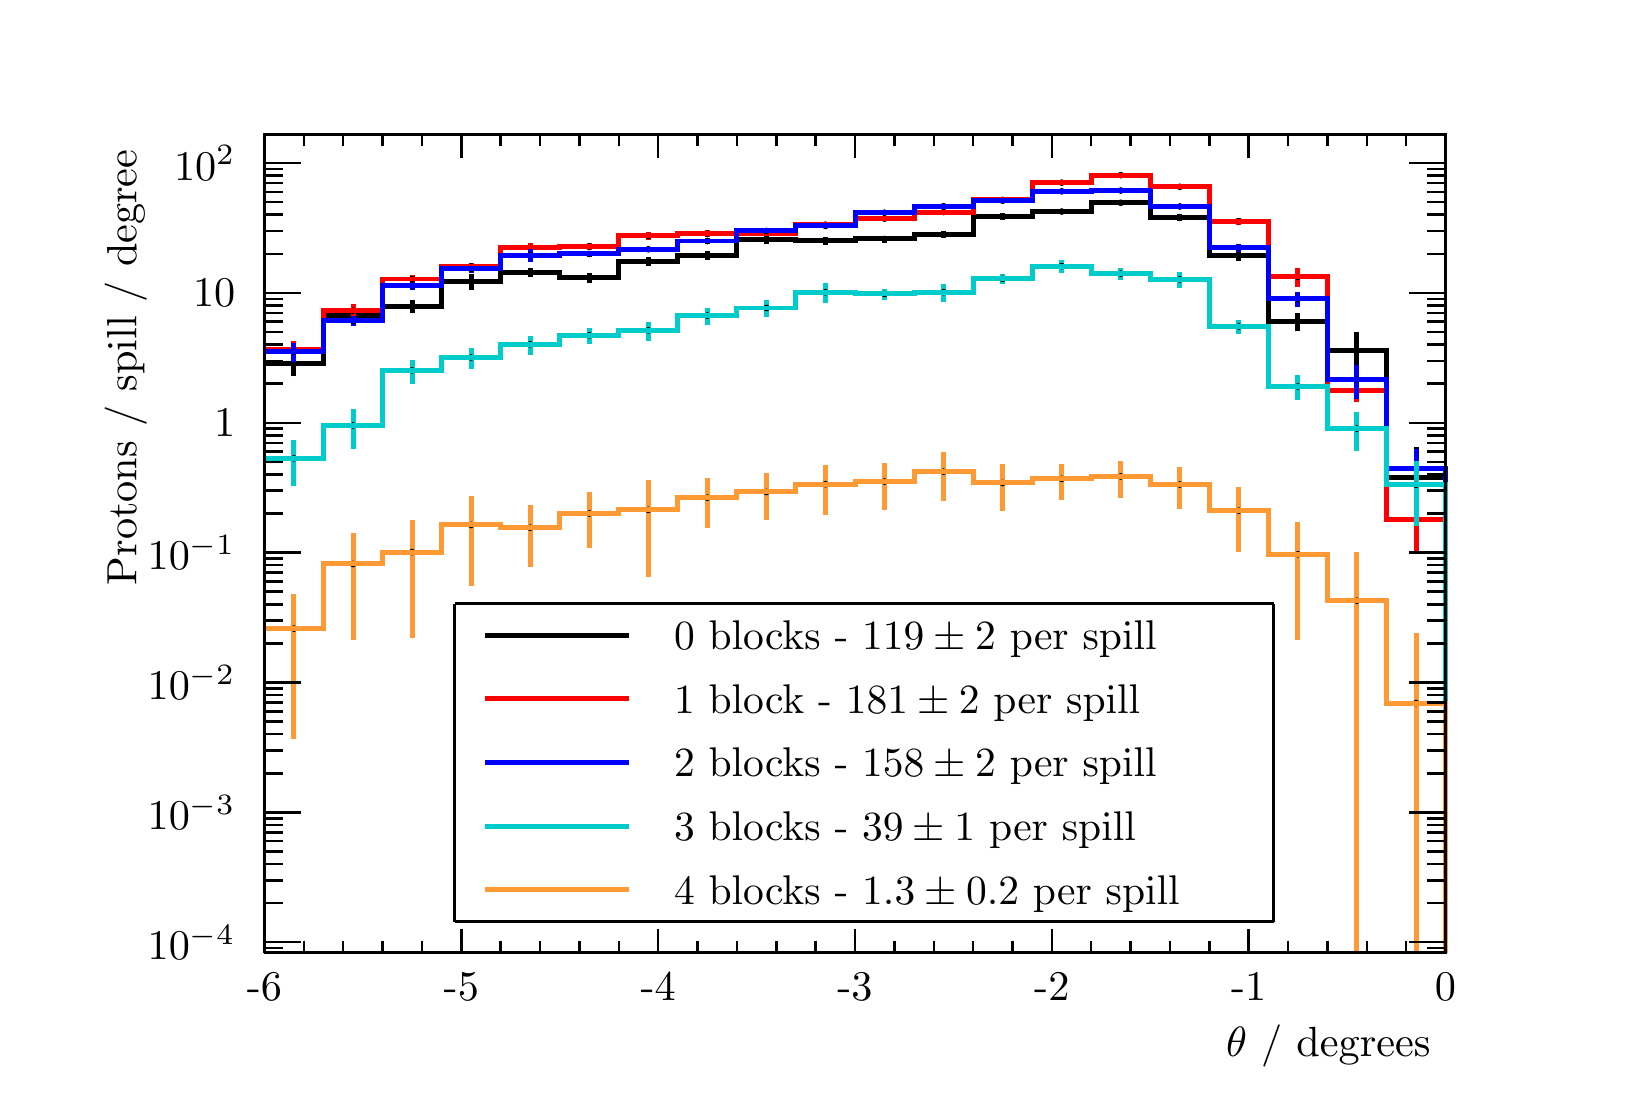
\begin{tikzpicture}
\pgfdeclareplotmark{cross} {
\pgfpathmoveto{\pgfpoint{-0.3\pgfplotmarksize}{\pgfplotmarksize}}
\pgfpathlineto{\pgfpoint{+0.3\pgfplotmarksize}{\pgfplotmarksize}}
\pgfpathlineto{\pgfpoint{+0.3\pgfplotmarksize}{0.3\pgfplotmarksize}}
\pgfpathlineto{\pgfpoint{+1\pgfplotmarksize}{0.3\pgfplotmarksize}}
\pgfpathlineto{\pgfpoint{+1\pgfplotmarksize}{-0.3\pgfplotmarksize}}
\pgfpathlineto{\pgfpoint{+0.3\pgfplotmarksize}{-0.3\pgfplotmarksize}}
\pgfpathlineto{\pgfpoint{+0.3\pgfplotmarksize}{-1.\pgfplotmarksize}}
\pgfpathlineto{\pgfpoint{-0.3\pgfplotmarksize}{-1.\pgfplotmarksize}}
\pgfpathlineto{\pgfpoint{-0.3\pgfplotmarksize}{-0.3\pgfplotmarksize}}
\pgfpathlineto{\pgfpoint{-1.\pgfplotmarksize}{-0.3\pgfplotmarksize}}
\pgfpathlineto{\pgfpoint{-1.\pgfplotmarksize}{0.3\pgfplotmarksize}}
\pgfpathlineto{\pgfpoint{-0.3\pgfplotmarksize}{0.3\pgfplotmarksize}}
\pgfpathclose
\pgfusepathqstroke
}
\pgfdeclareplotmark{cross*} {
\pgfpathmoveto{\pgfpoint{-0.3\pgfplotmarksize}{\pgfplotmarksize}}
\pgfpathlineto{\pgfpoint{+0.3\pgfplotmarksize}{\pgfplotmarksize}}
\pgfpathlineto{\pgfpoint{+0.3\pgfplotmarksize}{0.3\pgfplotmarksize}}
\pgfpathlineto{\pgfpoint{+1\pgfplotmarksize}{0.3\pgfplotmarksize}}
\pgfpathlineto{\pgfpoint{+1\pgfplotmarksize}{-0.3\pgfplotmarksize}}
\pgfpathlineto{\pgfpoint{+0.3\pgfplotmarksize}{-0.3\pgfplotmarksize}}
\pgfpathlineto{\pgfpoint{+0.3\pgfplotmarksize}{-1.\pgfplotmarksize}}
\pgfpathlineto{\pgfpoint{-0.3\pgfplotmarksize}{-1.\pgfplotmarksize}}
\pgfpathlineto{\pgfpoint{-0.3\pgfplotmarksize}{-0.3\pgfplotmarksize}}
\pgfpathlineto{\pgfpoint{-1.\pgfplotmarksize}{-0.3\pgfplotmarksize}}
\pgfpathlineto{\pgfpoint{-1.\pgfplotmarksize}{0.3\pgfplotmarksize}}
\pgfpathlineto{\pgfpoint{-0.3\pgfplotmarksize}{0.3\pgfplotmarksize}}
\pgfpathclose
\pgfusepathqfillstroke
}
\pgfdeclareplotmark{newstar} {
\pgfpathmoveto{\pgfqpoint{0pt}{\pgfplotmarksize}}
\pgfpathlineto{\pgfqpointpolar{44}{0.5\pgfplotmarksize}}
\pgfpathlineto{\pgfqpointpolar{18}{\pgfplotmarksize}}
\pgfpathlineto{\pgfqpointpolar{-20}{0.5\pgfplotmarksize}}
\pgfpathlineto{\pgfqpointpolar{-54}{\pgfplotmarksize}}
\pgfpathlineto{\pgfqpointpolar{-90}{0.5\pgfplotmarksize}}
\pgfpathlineto{\pgfqpointpolar{234}{\pgfplotmarksize}}
\pgfpathlineto{\pgfqpointpolar{198}{0.5\pgfplotmarksize}}
\pgfpathlineto{\pgfqpointpolar{162}{\pgfplotmarksize}}
\pgfpathlineto{\pgfqpointpolar{134}{0.5\pgfplotmarksize}}
\pgfpathclose
\pgfusepathqstroke
}
\pgfdeclareplotmark{newstar*} {
\pgfpathmoveto{\pgfqpoint{0pt}{\pgfplotmarksize}}
\pgfpathlineto{\pgfqpointpolar{44}{0.5\pgfplotmarksize}}
\pgfpathlineto{\pgfqpointpolar{18}{\pgfplotmarksize}}
\pgfpathlineto{\pgfqpointpolar{-20}{0.5\pgfplotmarksize}}
\pgfpathlineto{\pgfqpointpolar{-54}{\pgfplotmarksize}}
\pgfpathlineto{\pgfqpointpolar{-90}{0.5\pgfplotmarksize}}
\pgfpathlineto{\pgfqpointpolar{234}{\pgfplotmarksize}}
\pgfpathlineto{\pgfqpointpolar{198}{0.5\pgfplotmarksize}}
\pgfpathlineto{\pgfqpointpolar{162}{\pgfplotmarksize}}
\pgfpathlineto{\pgfqpointpolar{134}{0.5\pgfplotmarksize}}
\pgfpathclose
\pgfusepathqfillstroke
}
\definecolor{c}{rgb}{1,1,1};
\draw [color=c, fill=c] (0,0) rectangle (20,13.4957);
\draw [color=c, fill=c] (3,1.75444) rectangle (18,12.1461);
\definecolor{c}{rgb}{0,0,0};
\draw [c,line width=0.9] (3,1.75444) -- (3,12.1461) -- (18,12.1461) -- (18,1.75444) -- (3,1.75444);
\definecolor{c}{rgb}{1,1,1};
\draw [color=c, fill=c] (3,1.75444) rectangle (18,12.1461);
\definecolor{c}{rgb}{0,0,0};
\draw [c,line width=0.9] (3,1.75444) -- (3,12.1461) -- (18,12.1461) -- (18,1.75444) -- (3,1.75444);
\draw [c,line width=0.9] (3,1.75444) -- (3.75,1.75444) -- (3.75,1.75444) -- (4.5,1.75444) -- (4.5,1.75444) -- (5.25,1.75444) -- (5.25,1.75444) -- (6,1.75444) -- (6,1.75444) -- (6.75,1.75444) -- (6.75,1.75444) -- (7.5,1.75444) -- (7.5,1.75444) --
 (8.25,1.75444) -- (8.25,1.75444) -- (9,1.75444) -- (9,1.75444) -- (9.75,1.75444) -- (9.75,1.75444) -- (10.5,1.75444) -- (10.5,1.75444) -- (11.25,1.75444) -- (11.25,1.75444) -- (12,1.75444) -- (12,1.75444) -- (12.75,1.75444) -- (12.75,1.75444) --
 (13.5,1.75444) -- (13.5,1.75444) -- (14.25,1.75444) -- (14.25,1.75444) -- (15,1.75444) -- (15,1.75444) -- (15.75,1.75444) -- (15.75,1.75444) -- (16.5,1.75444) -- (16.5,1.75444) -- (17.25,1.75444) -- (17.25,1.75444) -- (18,1.75444) -- (18,1.75444);
\draw [c,line width=0.9] (3,1.75444) -- (18,1.75444);
\draw [c,line width=0.9] (3,2.05809) -- (3,1.75444);
\draw [c,line width=0.9] (3.5,1.90627) -- (3.5,1.75444);
\draw [c,line width=0.9] (4,1.90627) -- (4,1.75444);
\draw [c,line width=0.9] (4.5,1.90627) -- (4.5,1.75444);
\draw [c,line width=0.9] (5,1.90627) -- (5,1.75444);
\draw [c,line width=0.9] (5.5,2.05809) -- (5.5,1.75444);
\draw [c,line width=0.9] (6,1.90627) -- (6,1.75444);
\draw [c,line width=0.9] (6.5,1.90627) -- (6.5,1.75444);
\draw [c,line width=0.9] (7,1.90627) -- (7,1.75444);
\draw [c,line width=0.9] (7.5,1.90627) -- (7.5,1.75444);
\draw [c,line width=0.9] (8,2.05809) -- (8,1.75444);
\draw [c,line width=0.9] (8.5,1.90627) -- (8.5,1.75444);
\draw [c,line width=0.9] (9,1.90627) -- (9,1.75444);
\draw [c,line width=0.9] (9.5,1.90627) -- (9.5,1.75444);
\draw [c,line width=0.9] (10,1.90627) -- (10,1.75444);
\draw [c,line width=0.9] (10.5,2.05809) -- (10.5,1.75444);
\draw [c,line width=0.9] (11,1.90627) -- (11,1.75444);
\draw [c,line width=0.9] (11.5,1.90627) -- (11.5,1.75444);
\draw [c,line width=0.9] (12,1.90627) -- (12,1.75444);
\draw [c,line width=0.9] (12.5,1.90627) -- (12.5,1.75444);
\draw [c,line width=0.9] (13,2.05809) -- (13,1.75444);
\draw [c,line width=0.9] (13.5,1.90627) -- (13.5,1.75444);
\draw [c,line width=0.9] (14,1.90627) -- (14,1.75444);
\draw [c,line width=0.9] (14.5,1.90627) -- (14.5,1.75444);
\draw [c,line width=0.9] (15,1.90627) -- (15,1.75444);
\draw [c,line width=0.9] (15.5,2.05809) -- (15.5,1.75444);
\draw [c,line width=0.9] (16,1.90627) -- (16,1.75444);
\draw [c,line width=0.9] (16.5,1.90627) -- (16.5,1.75444);
\draw [c,line width=0.9] (17,1.90627) -- (17,1.75444);
\draw [c,line width=0.9] (17.5,1.90627) -- (17.5,1.75444);
\draw [c,line width=0.9] (18,2.05809) -- (18,1.75444);
\draw [anchor=base] (3,1.14713) node[scale=1.52731, color=c, rotate=0]{-6};
\draw [anchor=base] (5.5,1.14713) node[scale=1.52731, color=c, rotate=0]{-5};
\draw [anchor=base] (8,1.14713) node[scale=1.52731, color=c, rotate=0]{-4};
\draw [anchor=base] (10.5,1.14713) node[scale=1.52731, color=c, rotate=0]{-3};
\draw [anchor=base] (13,1.14713) node[scale=1.52731, color=c, rotate=0]{-2};
\draw [anchor=base] (15.5,1.14713) node[scale=1.52731, color=c, rotate=0]{-1};
\draw [anchor=base] (18,1.14713) node[scale=1.52731, color=c, rotate=0]{0};
\draw [anchor= east] (18,0.566819) node[scale=1.52731, color=c, rotate=0]{$ \theta$ / degrees};
\draw [c,line width=0.9] (3,12.1461) -- (18,12.1461);
\draw [c,line width=0.9] (3,11.8425) -- (3,12.1461);
\draw [c,line width=0.9] (3.5,11.9943) -- (3.5,12.1461);
\draw [c,line width=0.9] (4,11.9943) -- (4,12.1461);
\draw [c,line width=0.9] (4.5,11.9943) -- (4.5,12.1461);
\draw [c,line width=0.9] (5,11.9943) -- (5,12.1461);
\draw [c,line width=0.9] (5.5,11.8425) -- (5.5,12.1461);
\draw [c,line width=0.9] (6,11.9943) -- (6,12.1461);
\draw [c,line width=0.9] (6.5,11.9943) -- (6.5,12.1461);
\draw [c,line width=0.9] (7,11.9943) -- (7,12.1461);
\draw [c,line width=0.9] (7.5,11.9943) -- (7.5,12.1461);
\draw [c,line width=0.9] (8,11.8425) -- (8,12.1461);
\draw [c,line width=0.9] (8.5,11.9943) -- (8.5,12.1461);
\draw [c,line width=0.9] (9,11.9943) -- (9,12.1461);
\draw [c,line width=0.9] (9.5,11.9943) -- (9.5,12.1461);
\draw [c,line width=0.9] (10,11.9943) -- (10,12.1461);
\draw [c,line width=0.9] (10.5,11.8425) -- (10.5,12.1461);
\draw [c,line width=0.9] (11,11.9943) -- (11,12.1461);
\draw [c,line width=0.9] (11.5,11.9943) -- (11.5,12.1461);
\draw [c,line width=0.9] (12,11.9943) -- (12,12.1461);
\draw [c,line width=0.9] (12.5,11.9943) -- (12.5,12.1461);
\draw [c,line width=0.9] (13,11.8425) -- (13,12.1461);
\draw [c,line width=0.9] (13.5,11.9943) -- (13.5,12.1461);
\draw [c,line width=0.9] (14,11.9943) -- (14,12.1461);
\draw [c,line width=0.9] (14.5,11.9943) -- (14.5,12.1461);
\draw [c,line width=0.9] (15,11.9943) -- (15,12.1461);
\draw [c,line width=0.9] (15.5,11.8425) -- (15.5,12.1461);
\draw [c,line width=0.9] (16,11.9943) -- (16,12.1461);
\draw [c,line width=0.9] (16.5,11.9943) -- (16.5,12.1461);
\draw [c,line width=0.9] (17,11.9943) -- (17,12.1461);
\draw [c,line width=0.9] (17.5,11.9943) -- (17.5,12.1461);
\draw [c,line width=0.9] (18,11.8425) -- (18,12.1461);
\draw [c,line width=0.9] (3,1.75444) -- (3,12.1461);
\draw [c,line width=0.9] (3.231,1.81225) -- (3,1.81225);
\draw [c,line width=0.9] (3.462,1.88772) -- (3,1.88772);
\draw [anchor= east] (2.82,1.88772) node[scale=1.52731, color=c, rotate=0]{$10^{-4}$};
\draw [c,line width=0.9] (3.231,2.38422) -- (3,2.38422);
\draw [c,line width=0.9] (3.231,2.67466) -- (3,2.67466);
\draw [c,line width=0.9] (3.231,2.88072) -- (3,2.88072);
\draw [c,line width=0.9] (3.231,3.04056) -- (3,3.04056);
\draw [c,line width=0.9] (3.231,3.17116) -- (3,3.17116);
\draw [c,line width=0.9] (3.231,3.28158) -- (3,3.28158);
\draw [c,line width=0.9] (3.231,3.37722) -- (3,3.37722);
\draw [c,line width=0.9] (3.231,3.46159) -- (3,3.46159);
\draw [c,line width=0.9] (3.462,3.53706) -- (3,3.53706);
\draw [anchor= east] (2.82,3.53706) node[scale=1.52731, color=c, rotate=0]{$10^{-3}$};
\draw [c,line width=0.9] (3.231,4.03357) -- (3,4.03357);
\draw [c,line width=0.9] (3.231,4.324) -- (3,4.324);
\draw [c,line width=0.9] (3.231,4.53007) -- (3,4.53007);
\draw [c,line width=0.9] (3.231,4.68991) -- (3,4.68991);
\draw [c,line width=0.9] (3.231,4.8205) -- (3,4.8205);
\draw [c,line width=0.9] (3.231,4.93092) -- (3,4.93092);
\draw [c,line width=0.9] (3.231,5.02657) -- (3,5.02657);
\draw [c,line width=0.9] (3.231,5.11094) -- (3,5.11094);
\draw [c,line width=0.9] (3.462,5.18641) -- (3,5.18641);
\draw [anchor= east] (2.82,5.18641) node[scale=1.52731, color=c, rotate=0]{$10^{-2}$};
\draw [c,line width=0.9] (3.231,5.68291) -- (3,5.68291);
\draw [c,line width=0.9] (3.231,5.97335) -- (3,5.97335);
\draw [c,line width=0.9] (3.231,6.17941) -- (3,6.17941);
\draw [c,line width=0.9] (3.231,6.33925) -- (3,6.33925);
\draw [c,line width=0.9] (3.231,6.46985) -- (3,6.46985);
\draw [c,line width=0.9] (3.231,6.58027) -- (3,6.58027);
\draw [c,line width=0.9] (3.231,6.67592) -- (3,6.67592);
\draw [c,line width=0.9] (3.231,6.76028) -- (3,6.76028);
\draw [c,line width=0.9] (3.462,6.83575) -- (3,6.83575);
\draw [anchor= east] (2.82,6.83575) node[scale=1.52731, color=c, rotate=0]{$10^{-1}$};
\draw [c,line width=0.9] (3.231,7.33226) -- (3,7.33226);
\draw [c,line width=0.9] (3.231,7.62269) -- (3,7.62269);
\draw [c,line width=0.9] (3.231,7.82876) -- (3,7.82876);
\draw [c,line width=0.9] (3.231,7.9886) -- (3,7.9886);
\draw [c,line width=0.9] (3.231,8.11919) -- (3,8.11919);
\draw [c,line width=0.9] (3.231,8.22961) -- (3,8.22961);
\draw [c,line width=0.9] (3.231,8.32526) -- (3,8.32526);
\draw [c,line width=0.9] (3.231,8.40963) -- (3,8.40963);
\draw [c,line width=0.9] (3.462,8.4851) -- (3,8.4851);
\draw [anchor= east] (2.82,8.4851) node[scale=1.52731, color=c, rotate=0]{1};
\draw [c,line width=0.9] (3.231,8.9816) -- (3,8.9816);
\draw [c,line width=0.9] (3.231,9.27204) -- (3,9.27204);
\draw [c,line width=0.9] (3.231,9.4781) -- (3,9.4781);
\draw [c,line width=0.9] (3.231,9.63794) -- (3,9.63794);
\draw [c,line width=0.9] (3.231,9.76854) -- (3,9.76854);
\draw [c,line width=0.9] (3.231,9.87896) -- (3,9.87896);
\draw [c,line width=0.9] (3.231,9.97461) -- (3,9.97461);
\draw [c,line width=0.9] (3.231,10.059) -- (3,10.059);
\draw [c,line width=0.9] (3.462,10.1344) -- (3,10.1344);
\draw [anchor= east] (2.82,10.1344) node[scale=1.52731, color=c, rotate=0]{10};
\draw [c,line width=0.9] (3.231,10.6309) -- (3,10.6309);
\draw [c,line width=0.9] (3.231,10.9214) -- (3,10.9214);
\draw [c,line width=0.9] (3.231,11.1274) -- (3,11.1274);
\draw [c,line width=0.9] (3.231,11.2873) -- (3,11.2873);
\draw [c,line width=0.9] (3.231,11.4179) -- (3,11.4179);
\draw [c,line width=0.9] (3.231,11.5283) -- (3,11.5283);
\draw [c,line width=0.9] (3.231,11.624) -- (3,11.624);
\draw [c,line width=0.9] (3.231,11.7083) -- (3,11.7083);
\draw [c,line width=0.9] (3.462,11.7838) -- (3,11.7838);
\draw [anchor= east] (2.82,11.7838) node[scale=1.52731, color=c, rotate=0]{$10^{2}$};
\draw [anchor= east] (1.24,12.1461) node[scale=1.52731, color=c, rotate=90]{ Protons / spill / degree};
\draw [c,line width=0.9] (18,1.75444) -- (18,12.1461);
\draw [c,line width=0.9] (17.769,1.81225) -- (18,1.81225);
\draw [c,line width=0.9] (17.538,1.88772) -- (18,1.88772);
\draw [c,line width=0.9] (17.769,2.38422) -- (18,2.38422);
\draw [c,line width=0.9] (17.769,2.67466) -- (18,2.67466);
\draw [c,line width=0.9] (17.769,2.88072) -- (18,2.88072);
\draw [c,line width=0.9] (17.769,3.04056) -- (18,3.04056);
\draw [c,line width=0.9] (17.769,3.17116) -- (18,3.17116);
\draw [c,line width=0.9] (17.769,3.28158) -- (18,3.28158);
\draw [c,line width=0.9] (17.769,3.37722) -- (18,3.37722);
\draw [c,line width=0.9] (17.769,3.46159) -- (18,3.46159);
\draw [c,line width=0.9] (17.538,3.53706) -- (18,3.53706);
\draw [c,line width=0.9] (17.769,4.03357) -- (18,4.03357);
\draw [c,line width=0.9] (17.769,4.324) -- (18,4.324);
\draw [c,line width=0.9] (17.769,4.53007) -- (18,4.53007);
\draw [c,line width=0.9] (17.769,4.68991) -- (18,4.68991);
\draw [c,line width=0.9] (17.769,4.8205) -- (18,4.8205);
\draw [c,line width=0.9] (17.769,4.93092) -- (18,4.93092);
\draw [c,line width=0.9] (17.769,5.02657) -- (18,5.02657);
\draw [c,line width=0.9] (17.769,5.11094) -- (18,5.11094);
\draw [c,line width=0.9] (17.538,5.18641) -- (18,5.18641);
\draw [c,line width=0.9] (17.769,5.68291) -- (18,5.68291);
\draw [c,line width=0.9] (17.769,5.97335) -- (18,5.97335);
\draw [c,line width=0.9] (17.769,6.17941) -- (18,6.17941);
\draw [c,line width=0.9] (17.769,6.33925) -- (18,6.33925);
\draw [c,line width=0.9] (17.769,6.46985) -- (18,6.46985);
\draw [c,line width=0.9] (17.769,6.58027) -- (18,6.58027);
\draw [c,line width=0.9] (17.769,6.67592) -- (18,6.67592);
\draw [c,line width=0.9] (17.769,6.76028) -- (18,6.76028);
\draw [c,line width=0.9] (17.538,6.83575) -- (18,6.83575);
\draw [c,line width=0.9] (17.769,7.33226) -- (18,7.33226);
\draw [c,line width=0.9] (17.769,7.62269) -- (18,7.62269);
\draw [c,line width=0.9] (17.769,7.82876) -- (18,7.82876);
\draw [c,line width=0.9] (17.769,7.9886) -- (18,7.9886);
\draw [c,line width=0.9] (17.769,8.11919) -- (18,8.11919);
\draw [c,line width=0.9] (17.769,8.22961) -- (18,8.22961);
\draw [c,line width=0.9] (17.769,8.32526) -- (18,8.32526);
\draw [c,line width=0.9] (17.769,8.40963) -- (18,8.40963);
\draw [c,line width=0.9] (17.538,8.4851) -- (18,8.4851);
\draw [c,line width=0.9] (17.769,8.9816) -- (18,8.9816);
\draw [c,line width=0.9] (17.769,9.27204) -- (18,9.27204);
\draw [c,line width=0.9] (17.769,9.4781) -- (18,9.4781);
\draw [c,line width=0.9] (17.769,9.63794) -- (18,9.63794);
\draw [c,line width=0.9] (17.769,9.76854) -- (18,9.76854);
\draw [c,line width=0.9] (17.769,9.87896) -- (18,9.87896);
\draw [c,line width=0.9] (17.769,9.97461) -- (18,9.97461);
\draw [c,line width=0.9] (17.769,10.059) -- (18,10.059);
\draw [c,line width=0.9] (17.538,10.1344) -- (18,10.1344);
\draw [c,line width=0.9] (17.769,10.6309) -- (18,10.6309);
\draw [c,line width=0.9] (17.769,10.9214) -- (18,10.9214);
\draw [c,line width=0.9] (17.769,11.1274) -- (18,11.1274);
\draw [c,line width=0.9] (17.769,11.2873) -- (18,11.2873);
\draw [c,line width=0.9] (17.769,11.4179) -- (18,11.4179);
\draw [c,line width=0.9] (17.769,11.5283) -- (18,11.5283);
\draw [c,line width=0.9] (17.769,11.624) -- (18,11.624);
\draw [c,line width=0.9] (17.769,11.7083) -- (18,11.7083);
\draw [c,line width=0.9] (17.538,11.7838) -- (18,11.7838);
\draw [c,line width=1.8] (3.375,9.07502) -- (3.375,9.23213);
\draw [c,line width=1.8] (3.375,9.23213) -- (3.375,9.3609);
\foreach \P in {(3.375,9.23213)}{\draw[mark options={color=c,fill=c},mark size=2.402402pt,mark=*,mark size=1pt] plot coordinates {\P};}
\draw [c,line width=1.8] (4.125,9.75966) -- (4.125,9.85284);
\draw [c,line width=1.8] (4.125,9.85284) -- (4.125,9.93528);
\foreach \P in {(4.125,9.85284)}{\draw[mark options={color=c,fill=c},mark size=2.402402pt,mark=*,mark size=1pt] plot coordinates {\P};}
\draw [c,line width=1.8] (4.875,9.87682) -- (4.875,9.96395);
\draw [c,line width=1.8] (4.875,9.96395) -- (4.875,10.0416);
\foreach \P in {(4.875,9.96395)}{\draw[mark options={color=c,fill=c},mark size=2.402402pt,mark=*,mark size=1pt] plot coordinates {\P};}
\draw [c,line width=1.8] (5.625,10.1726) -- (5.625,10.2788);
\draw [c,line width=1.8] (5.625,10.2788) -- (5.625,10.3713);
\foreach \P in {(5.625,10.2788)}{\draw[mark options={color=c,fill=c},mark size=2.402402pt,mark=*,mark size=1pt] plot coordinates {\P};}
\draw [c,line width=1.8] (6.375,10.3373) -- (6.375,10.3992);
\draw [c,line width=1.8] (6.375,10.3992) -- (6.375,10.4562);
\foreach \P in {(6.375,10.3992)}{\draw[mark options={color=c,fill=c},mark size=2.402402pt,mark=*,mark size=1pt] plot coordinates {\P};}
\draw [c,line width=1.8] (7.125,10.2656) -- (7.125,10.3311);
\draw [c,line width=1.8] (7.125,10.3311) -- (7.125,10.3911);
\foreach \P in {(7.125,10.3311)}{\draw[mark options={color=c,fill=c},mark size=2.402402pt,mark=*,mark size=1pt] plot coordinates {\P};}
\draw [c,line width=1.8] (7.875,10.4763) -- (7.875,10.5374);
\draw [c,line width=1.8] (7.875,10.5374) -- (7.875,10.5938);
\foreach \P in {(7.875,10.5374)}{\draw[mark options={color=c,fill=c},mark size=2.402402pt,mark=*,mark size=1pt] plot coordinates {\P};}
\draw [c,line width=1.8] (8.625,10.5567) -- (8.625,10.6116);
\draw [c,line width=1.8] (8.625,10.6116) -- (8.625,10.6626);
\foreach \P in {(8.625,10.6116)}{\draw[mark options={color=c,fill=c},mark size=2.402402pt,mark=*,mark size=1pt] plot coordinates {\P};}
\draw [c,line width=1.8] (9.375,10.7503) -- (9.375,10.8141);
\draw [c,line width=1.8] (9.375,10.8141) -- (9.375,10.8726);
\foreach \P in {(9.375,10.8141)}{\draw[mark options={color=c,fill=c},mark size=2.402402pt,mark=*,mark size=1pt] plot coordinates {\P};}
\draw [c,line width=1.8] (10.125,10.7469) -- (10.125,10.7963);
\draw [c,line width=1.8] (10.125,10.7963) -- (10.125,10.8425);
\foreach \P in {(10.125,10.7963)}{\draw[mark options={color=c,fill=c},mark size=2.402402pt,mark=*,mark size=1pt] plot coordinates {\P};}
\draw [c,line width=1.8] (10.875,10.7735) -- (10.875,10.8191);
\draw [c,line width=1.8] (10.875,10.8191) -- (10.875,10.8619);
\foreach \P in {(10.875,10.8191)}{\draw[mark options={color=c,fill=c},mark size=2.402402pt,mark=*,mark size=1pt] plot coordinates {\P};}
\draw [c,line width=1.8] (11.625,10.8337) -- (11.625,10.877);
\draw [c,line width=1.8] (11.625,10.877) -- (11.625,10.9179);
\foreach \P in {(11.625,10.877)}{\draw[mark options={color=c,fill=c},mark size=2.402402pt,mark=*,mark size=1pt] plot coordinates {\P};}
\draw [c,line width=1.8] (12.375,11.0626) -- (12.375,11.1046);
\draw [c,line width=1.8] (12.375,11.1046) -- (12.375,11.1444);
\foreach \P in {(12.375,11.1046)}{\draw[mark options={color=c,fill=c},mark size=2.402402pt,mark=*,mark size=1pt] plot coordinates {\P};}
\draw [c,line width=1.8] (13.125,11.1339) -- (13.125,11.1675);
\draw [c,line width=1.8] (13.125,11.1675) -- (13.125,11.1996);
\foreach \P in {(13.125,11.1675)}{\draw[mark options={color=c,fill=c},mark size=2.402402pt,mark=*,mark size=1pt] plot coordinates {\P};}
\draw [c,line width=1.8] (13.875,11.2461) -- (13.875,11.2785);
\draw [c,line width=1.8] (13.875,11.2785) -- (13.875,11.3096);
\foreach \P in {(13.875,11.2785)}{\draw[mark options={color=c,fill=c},mark size=2.402402pt,mark=*,mark size=1pt] plot coordinates {\P};}
\draw [c,line width=1.8] (14.625,11.0483) -- (14.625,11.0912);
\draw [c,line width=1.8] (14.625,11.0912) -- (14.625,11.1317);
\foreach \P in {(14.625,11.0912)}{\draw[mark options={color=c,fill=c},mark size=2.402402pt,mark=*,mark size=1pt] plot coordinates {\P};}
\draw [c,line width=1.8] (15.375,10.5449) -- (15.375,10.608);
\draw [c,line width=1.8] (15.375,10.608) -- (15.375,10.666);
\foreach \P in {(15.375,10.608)}{\draw[mark options={color=c,fill=c},mark size=2.402402pt,mark=*,mark size=1pt] plot coordinates {\P};}
\draw [c,line width=1.8] (16.125,9.64718) -- (16.125,9.77334);
\draw [c,line width=1.8] (16.125,9.77334) -- (16.125,9.88057);
\foreach \P in {(16.125,9.77334)}{\draw[mark options={color=c,fill=c},mark size=2.402402pt,mark=*,mark size=1pt] plot coordinates {\P};}
\draw [c,line width=1.8] (16.875,9.05435) -- (16.875,9.40081);
\draw [c,line width=1.8] (16.875,9.40081) -- (16.875,9.63333);
\foreach \P in {(16.875,9.40081)}{\draw[mark options={color=c,fill=c},mark size=2.402402pt,mark=*,mark size=1pt] plot coordinates {\P};}
\draw [c,line width=1.8] (17.625,6.89102) -- (17.625,7.79455);
\draw [c,line width=1.8] (17.625,7.79455) -- (17.625,8.18165);
\foreach \P in {(17.625,7.79455)}{\draw[mark options={color=c,fill=c},mark size=2.402402pt,mark=*,mark size=1pt] plot coordinates {\P};}
\draw [c,line width=1.8] (3,9.23213) -- (3.75,9.23213) -- (3.75,9.85284) -- (4.5,9.85284) -- (4.5,9.96395) -- (5.25,9.96395) -- (5.25,10.2788) -- (6,10.2788) -- (6,10.3992) -- (6.75,10.3992) -- (6.75,10.3311) -- (7.5,10.3311) -- (7.5,10.5374) --
 (8.25,10.5374) -- (8.25,10.6116) -- (9,10.6116) -- (9,10.8141) -- (9.75,10.8141) -- (9.75,10.7963) -- (10.5,10.7963) -- (10.5,10.8191) -- (11.25,10.8191) -- (11.25,10.877) -- (12,10.877) -- (12,11.1046) -- (12.75,11.1046) -- (12.75,11.1675) --
 (13.5,11.1675) -- (13.5,11.2785) -- (14.25,11.2785) -- (14.25,11.0912) -- (15,11.0912) -- (15,10.608) -- (15.75,10.608) -- (15.75,9.77334) -- (16.5,9.77334) -- (16.5,9.40081) -- (17.25,9.40081) -- (17.25,7.79455) -- (18,7.79455) -- (18,1.75444);
\definecolor{c}{rgb}{1,0,0};
\draw [c,line width=1.8] (3.375,9.29318) -- (3.375,9.41497);
\draw [c,line width=1.8] (3.375,9.41497) -- (3.375,9.51902);
\definecolor{c}{rgb}{0,0,0};
\foreach \P in {(3.375,9.41497)}{\draw[mark options={color=c,fill=c},mark size=2.402402pt,mark=*,mark size=1pt] plot coordinates {\P};}
\definecolor{c}{rgb}{1,0,0};
\draw [c,line width=1.8] (4.125,9.80481) -- (4.125,9.90725);
\draw [c,line width=1.8] (4.125,9.90725) -- (4.125,9.99686);
\definecolor{c}{rgb}{0,0,0};
\foreach \P in {(4.125,9.90725)}{\draw[mark options={color=c,fill=c},mark size=2.402402pt,mark=*,mark size=1pt] plot coordinates {\P};}
\definecolor{c}{rgb}{1,0,0};
\draw [c,line width=1.8] (4.875,10.249) -- (4.875,10.3108);
\draw [c,line width=1.8] (4.875,10.3108) -- (4.875,10.3677);
\definecolor{c}{rgb}{0,0,0};
\foreach \P in {(4.875,10.3108)}{\draw[mark options={color=c,fill=c},mark size=2.402402pt,mark=*,mark size=1pt] plot coordinates {\P};}
\definecolor{c}{rgb}{1,0,0};
\draw [c,line width=1.8] (5.625,10.4221) -- (5.625,10.4723);
\draw [c,line width=1.8] (5.625,10.4723) -- (5.625,10.5191);
\definecolor{c}{rgb}{0,0,0};
\foreach \P in {(5.625,10.4723)}{\draw[mark options={color=c,fill=c},mark size=2.402402pt,mark=*,mark size=1pt] plot coordinates {\P};}
\definecolor{c}{rgb}{1,0,0};
\draw [c,line width=1.8] (6.375,10.6326) -- (6.375,10.7055);
\draw [c,line width=1.8] (6.375,10.7055) -- (6.375,10.7716);
\definecolor{c}{rgb}{0,0,0};
\foreach \P in {(6.375,10.7055)}{\draw[mark options={color=c,fill=c},mark size=2.402402pt,mark=*,mark size=1pt] plot coordinates {\P};}
\definecolor{c}{rgb}{1,0,0};
\draw [c,line width=1.8] (7.125,10.6743) -- (7.125,10.7239);
\draw [c,line width=1.8] (7.125,10.7239) -- (7.125,10.7702);
\definecolor{c}{rgb}{0,0,0};
\foreach \P in {(7.125,10.7239)}{\draw[mark options={color=c,fill=c},mark size=2.402402pt,mark=*,mark size=1pt] plot coordinates {\P};}
\definecolor{c}{rgb}{1,0,0};
\draw [c,line width=1.8] (7.875,10.8026) -- (7.875,10.8576);
\draw [c,line width=1.8] (7.875,10.8576) -- (7.875,10.9087);
\definecolor{c}{rgb}{0,0,0};
\foreach \P in {(7.875,10.8576)}{\draw[mark options={color=c,fill=c},mark size=2.402402pt,mark=*,mark size=1pt] plot coordinates {\P};}
\definecolor{c}{rgb}{1,0,0};
\draw [c,line width=1.8] (8.625,10.8427) -- (8.625,10.8862);
\draw [c,line width=1.8] (8.625,10.8862) -- (8.625,10.9272);
\definecolor{c}{rgb}{0,0,0};
\foreach \P in {(8.625,10.8862)}{\draw[mark options={color=c,fill=c},mark size=2.402402pt,mark=*,mark size=1pt] plot coordinates {\P};}
\definecolor{c}{rgb}{1,0,0};
\draw [c,line width=1.8] (9.375,10.8581) -- (9.375,10.8913);
\draw [c,line width=1.8] (9.375,10.8913) -- (9.375,10.923);
\definecolor{c}{rgb}{0,0,0};
\foreach \P in {(9.375,10.8913)}{\draw[mark options={color=c,fill=c},mark size=2.402402pt,mark=*,mark size=1pt] plot coordinates {\P};}
\definecolor{c}{rgb}{1,0,0};
\draw [c,line width=1.8] (10.125,10.9658) -- (10.125,11.0008);
\draw [c,line width=1.8] (10.125,11.0008) -- (10.125,11.0341);
\definecolor{c}{rgb}{0,0,0};
\foreach \P in {(10.125,11.0008)}{\draw[mark options={color=c,fill=c},mark size=2.402402pt,mark=*,mark size=1pt] plot coordinates {\P};}
\definecolor{c}{rgb}{1,0,0};
\draw [c,line width=1.8] (10.875,11.0434) -- (10.875,11.0777);
\draw [c,line width=1.8] (10.875,11.0777) -- (10.875,11.1105);
\definecolor{c}{rgb}{0,0,0};
\foreach \P in {(10.875,11.0777)}{\draw[mark options={color=c,fill=c},mark size=2.402402pt,mark=*,mark size=1pt] plot coordinates {\P};}
\definecolor{c}{rgb}{1,0,0};
\draw [c,line width=1.8] (11.625,11.1321) -- (11.625,11.1615);
\draw [c,line width=1.8] (11.625,11.1615) -- (11.625,11.1898);
\definecolor{c}{rgb}{0,0,0};
\foreach \P in {(11.625,11.1615)}{\draw[mark options={color=c,fill=c},mark size=2.402402pt,mark=*,mark size=1pt] plot coordinates {\P};}
\definecolor{c}{rgb}{1,0,0};
\draw [c,line width=1.8] (12.375,11.2866) -- (12.375,11.3151);
\draw [c,line width=1.8] (12.375,11.3151) -- (12.375,11.3425);
\definecolor{c}{rgb}{0,0,0};
\foreach \P in {(12.375,11.3151)}{\draw[mark options={color=c,fill=c},mark size=2.402402pt,mark=*,mark size=1pt] plot coordinates {\P};}
\definecolor{c}{rgb}{1,0,0};
\draw [c,line width=1.8] (13.125,11.5124) -- (13.125,11.5342);
\draw [c,line width=1.8] (13.125,11.5342) -- (13.125,11.5554);
\definecolor{c}{rgb}{0,0,0};
\foreach \P in {(13.125,11.5342)}{\draw[mark options={color=c,fill=c},mark size=2.402402pt,mark=*,mark size=1pt] plot coordinates {\P};}
\definecolor{c}{rgb}{1,0,0};
\draw [c,line width=1.8] (13.875,11.6021) -- (13.875,11.6298);
\draw [c,line width=1.8] (13.875,11.6298) -- (13.875,11.6565);
\definecolor{c}{rgb}{0,0,0};
\foreach \P in {(13.875,11.6298)}{\draw[mark options={color=c,fill=c},mark size=2.402402pt,mark=*,mark size=1pt] plot coordinates {\P};}
\definecolor{c}{rgb}{1,0,0};
\draw [c,line width=1.8] (14.625,11.4519) -- (14.625,11.4816);
\draw [c,line width=1.8] (14.625,11.4816) -- (14.625,11.51);
\definecolor{c}{rgb}{0,0,0};
\foreach \P in {(14.625,11.4816)}{\draw[mark options={color=c,fill=c},mark size=2.402402pt,mark=*,mark size=1pt] plot coordinates {\P};}
\definecolor{c}{rgb}{1,0,0};
\draw [c,line width=1.8] (15.375,10.9998) -- (15.375,11.0445);
\draw [c,line width=1.8] (15.375,11.0445) -- (15.375,11.0866);
\definecolor{c}{rgb}{0,0,0};
\foreach \P in {(15.375,11.0445)}{\draw[mark options={color=c,fill=c},mark size=2.402402pt,mark=*,mark size=1pt] plot coordinates {\P};}
\definecolor{c}{rgb}{1,0,0};
\draw [c,line width=1.8] (16.125,10.2048) -- (16.125,10.3367);
\draw [c,line width=1.8] (16.125,10.3367) -- (16.125,10.4481);
\definecolor{c}{rgb}{0,0,0};
\foreach \P in {(16.125,10.3367)}{\draw[mark options={color=c,fill=c},mark size=2.402402pt,mark=*,mark size=1pt] plot coordinates {\P};}
\definecolor{c}{rgb}{1,0,0};
\draw [c,line width=1.8] (16.875,8.75069) -- (16.875,8.89064);
\draw [c,line width=1.8] (16.875,8.89064) -- (16.875,9.00767);
\definecolor{c}{rgb}{0,0,0};
\foreach \P in {(16.875,8.89064)}{\draw[mark options={color=c,fill=c},mark size=2.402402pt,mark=*,mark size=1pt] plot coordinates {\P};}
\definecolor{c}{rgb}{1,0,0};
\draw [c,line width=1.8] (17.625,6.83079) -- (17.625,7.25361);
\draw [c,line width=1.8] (17.625,7.25361) -- (17.625,7.51769);
\definecolor{c}{rgb}{0,0,0};
\foreach \P in {(17.625,7.25361)}{\draw[mark options={color=c,fill=c},mark size=2.402402pt,mark=*,mark size=1pt] plot coordinates {\P};}
\definecolor{c}{rgb}{1,0,0};
\draw [c,line width=1.8] (3,9.41497) -- (3.75,9.41497) -- (3.75,9.90725) -- (4.5,9.90725) -- (4.5,10.3108) -- (5.25,10.3108) -- (5.25,10.4723) -- (6,10.4723) -- (6,10.7055) -- (6.75,10.7055) -- (6.75,10.7239) -- (7.5,10.7239) -- (7.5,10.8576) --
 (8.25,10.8576) -- (8.25,10.8862) -- (9,10.8862) -- (9,10.8913) -- (9.75,10.8913) -- (9.75,11.0008) -- (10.5,11.0008) -- (10.5,11.0777) -- (11.25,11.0777) -- (11.25,11.1615) -- (12,11.1615) -- (12,11.3151) -- (12.75,11.3151) -- (12.75,11.5342) --
 (13.5,11.5342) -- (13.5,11.6298) -- (14.25,11.6298) -- (14.25,11.4816) -- (15,11.4816) -- (15,11.0445) -- (15.75,11.0445) -- (15.75,10.3367) -- (16.5,10.3367) -- (16.5,8.89064) -- (17.25,8.89064) -- (17.25,7.25361) -- (18,7.25361) -- (18,1.75444);
\definecolor{c}{rgb}{0,0,1};
\draw [c,line width=1.8] (3.375,9.26219) -- (3.375,9.38668);
\draw [c,line width=1.8] (3.375,9.38668) -- (3.375,9.4927);
\definecolor{c}{rgb}{0,0,0};
\foreach \P in {(3.375,9.38668)}{\draw[mark options={color=c,fill=c},mark size=2.402402pt,mark=*,mark size=1pt] plot coordinates {\P};}
\definecolor{c}{rgb}{0,0,1};
\draw [c,line width=1.8] (4.125,9.70904) -- (4.125,9.77916);
\draw [c,line width=1.8] (4.125,9.77916) -- (4.125,9.84303);
\definecolor{c}{rgb}{0,0,0};
\foreach \P in {(4.125,9.77916)}{\draw[mark options={color=c,fill=c},mark size=2.402402pt,mark=*,mark size=1pt] plot coordinates {\P};}
\definecolor{c}{rgb}{0,0,1};
\draw [c,line width=1.8] (4.875,10.1747) -- (4.875,10.2284);
\draw [c,line width=1.8] (4.875,10.2284) -- (4.875,10.2784);
\definecolor{c}{rgb}{0,0,0};
\foreach \P in {(4.875,10.2284)}{\draw[mark options={color=c,fill=c},mark size=2.402402pt,mark=*,mark size=1pt] plot coordinates {\P};}
\definecolor{c}{rgb}{0,0,1};
\draw [c,line width=1.8] (5.625,10.3923) -- (5.625,10.4383);
\draw [c,line width=1.8] (5.625,10.4383) -- (5.625,10.4816);
\definecolor{c}{rgb}{0,0,0};
\foreach \P in {(5.625,10.4383)}{\draw[mark options={color=c,fill=c},mark size=2.402402pt,mark=*,mark size=1pt] plot coordinates {\P};}
\definecolor{c}{rgb}{0,0,1};
\draw [c,line width=1.8] (6.375,10.5222) -- (6.375,10.6123);
\draw [c,line width=1.8] (6.375,10.6123) -- (6.375,10.6922);
\definecolor{c}{rgb}{0,0,0};
\foreach \P in {(6.375,10.6123)}{\draw[mark options={color=c,fill=c},mark size=2.402402pt,mark=*,mark size=1pt] plot coordinates {\P};}
\definecolor{c}{rgb}{0,0,1};
\draw [c,line width=1.8] (7.125,10.5909) -- (7.125,10.629);
\draw [c,line width=1.8] (7.125,10.629) -- (7.125,10.6652);
\definecolor{c}{rgb}{0,0,0};
\foreach \P in {(7.125,10.629)}{\draw[mark options={color=c,fill=c},mark size=2.402402pt,mark=*,mark size=1pt] plot coordinates {\P};}
\definecolor{c}{rgb}{0,0,1};
\draw [c,line width=1.8] (7.875,10.6551) -- (7.875,10.6884);
\draw [c,line width=1.8] (7.875,10.6884) -- (7.875,10.7202);
\definecolor{c}{rgb}{0,0,0};
\foreach \P in {(7.875,10.6884)}{\draw[mark options={color=c,fill=c},mark size=2.402402pt,mark=*,mark size=1pt] plot coordinates {\P};}
\definecolor{c}{rgb}{0,0,1};
\draw [c,line width=1.8] (8.625,10.76) -- (8.625,10.7933);
\draw [c,line width=1.8] (8.625,10.7933) -- (8.625,10.8251);
\definecolor{c}{rgb}{0,0,0};
\foreach \P in {(8.625,10.7933)}{\draw[mark options={color=c,fill=c},mark size=2.402402pt,mark=*,mark size=1pt] plot coordinates {\P};}
\definecolor{c}{rgb}{0,0,1};
\draw [c,line width=1.8] (9.375,10.888) -- (9.375,10.9207);
\draw [c,line width=1.8] (9.375,10.9207) -- (9.375,10.952);
\definecolor{c}{rgb}{0,0,0};
\foreach \P in {(9.375,10.9207)}{\draw[mark options={color=c,fill=c},mark size=2.402402pt,mark=*,mark size=1pt] plot coordinates {\P};}
\definecolor{c}{rgb}{0,0,1};
\draw [c,line width=1.8] (10.125,10.9536) -- (10.125,10.985);
\draw [c,line width=1.8] (10.125,10.985) -- (10.125,11.015);
\definecolor{c}{rgb}{0,0,0};
\foreach \P in {(10.125,10.985)}{\draw[mark options={color=c,fill=c},mark size=2.402402pt,mark=*,mark size=1pt] plot coordinates {\P};}
\definecolor{c}{rgb}{0,0,1};
\draw [c,line width=1.8] (10.875,11.1223) -- (10.875,11.1525);
\draw [c,line width=1.8] (10.875,11.1525) -- (10.875,11.1815);
\definecolor{c}{rgb}{0,0,0};
\foreach \P in {(10.875,11.1525)}{\draw[mark options={color=c,fill=c},mark size=2.402402pt,mark=*,mark size=1pt] plot coordinates {\P};}
\definecolor{c}{rgb}{0,0,1};
\draw [c,line width=1.8] (11.625,11.2075) -- (11.625,11.2349);
\draw [c,line width=1.8] (11.625,11.2349) -- (11.625,11.2612);
\definecolor{c}{rgb}{0,0,0};
\foreach \P in {(11.625,11.2349)}{\draw[mark options={color=c,fill=c},mark size=2.402402pt,mark=*,mark size=1pt] plot coordinates {\P};}
\definecolor{c}{rgb}{0,0,1};
\draw [c,line width=1.8] (12.375,11.2803) -- (12.375,11.3051);
\draw [c,line width=1.8] (12.375,11.3051) -- (12.375,11.329);
\definecolor{c}{rgb}{0,0,0};
\foreach \P in {(12.375,11.3051)}{\draw[mark options={color=c,fill=c},mark size=2.402402pt,mark=*,mark size=1pt] plot coordinates {\P};}
\definecolor{c}{rgb}{0,0,1};
\draw [c,line width=1.8] (13.125,11.4016) -- (13.125,11.4237);
\draw [c,line width=1.8] (13.125,11.4237) -- (13.125,11.4451);
\definecolor{c}{rgb}{0,0,0};
\foreach \P in {(13.125,11.4237)}{\draw[mark options={color=c,fill=c},mark size=2.402402pt,mark=*,mark size=1pt] plot coordinates {\P};}
\definecolor{c}{rgb}{0,0,1};
\draw [c,line width=1.8] (13.875,11.4097) -- (13.875,11.4344);
\draw [c,line width=1.8] (13.875,11.4344) -- (13.875,11.4582);
\definecolor{c}{rgb}{0,0,0};
\foreach \P in {(13.875,11.4344)}{\draw[mark options={color=c,fill=c},mark size=2.402402pt,mark=*,mark size=1pt] plot coordinates {\P};}
\definecolor{c}{rgb}{0,0,1};
\draw [c,line width=1.8] (14.625,11.2014) -- (14.625,11.2318);
\draw [c,line width=1.8] (14.625,11.2318) -- (14.625,11.2609);
\definecolor{c}{rgb}{0,0,0};
\foreach \P in {(14.625,11.2318)}{\draw[mark options={color=c,fill=c},mark size=2.402402pt,mark=*,mark size=1pt] plot coordinates {\P};}
\definecolor{c}{rgb}{0,0,1};
\draw [c,line width=1.8] (15.375,10.6577) -- (15.375,10.7085);
\draw [c,line width=1.8] (15.375,10.7085) -- (15.375,10.756);
\definecolor{c}{rgb}{0,0,0};
\foreach \P in {(15.375,10.7085)}{\draw[mark options={color=c,fill=c},mark size=2.402402pt,mark=*,mark size=1pt] plot coordinates {\P};}
\definecolor{c}{rgb}{0,0,1};
\draw [c,line width=1.8] (16.125,9.9559) -- (16.125,10.0573);
\draw [c,line width=1.8] (16.125,10.0573) -- (16.125,10.1462);
\definecolor{c}{rgb}{0,0,0};
\foreach \P in {(16.125,10.0573)}{\draw[mark options={color=c,fill=c},mark size=2.402402pt,mark=*,mark size=1pt] plot coordinates {\P};}
\definecolor{c}{rgb}{0,0,1};
\draw [c,line width=1.8] (16.875,8.7896) -- (16.875,9.03343);
\draw [c,line width=1.8] (16.875,9.03343) -- (16.875,9.21501);
\definecolor{c}{rgb}{0,0,0};
\foreach \P in {(16.875,9.03343)}{\draw[mark options={color=c,fill=c},mark size=2.402402pt,mark=*,mark size=1pt] plot coordinates {\P};}
\definecolor{c}{rgb}{0,0,1};
\draw [c,line width=1.8] (17.625,7.50684) -- (17.625,7.89908);
\draw [c,line width=1.8] (17.625,7.89908) -- (17.625,8.15109);
\definecolor{c}{rgb}{0,0,0};
\foreach \P in {(17.625,7.89908)}{\draw[mark options={color=c,fill=c},mark size=2.402402pt,mark=*,mark size=1pt] plot coordinates {\P};}
\definecolor{c}{rgb}{0,0,1};
\draw [c,line width=1.8] (3,9.38668) -- (3.75,9.38668) -- (3.75,9.77916) -- (4.5,9.77916) -- (4.5,10.2284) -- (5.25,10.2284) -- (5.25,10.4383) -- (6,10.4383) -- (6,10.6123) -- (6.75,10.6123) -- (6.75,10.629) -- (7.5,10.629) -- (7.5,10.6884) --
 (8.25,10.6884) -- (8.25,10.7933) -- (9,10.7933) -- (9,10.9207) -- (9.75,10.9207) -- (9.75,10.985) -- (10.5,10.985) -- (10.5,11.1525) -- (11.25,11.1525) -- (11.25,11.2349) -- (12,11.2349) -- (12,11.3051) -- (12.75,11.3051) -- (12.75,11.4237) --
 (13.5,11.4237) -- (13.5,11.4344) -- (14.25,11.4344) -- (14.25,11.2318) -- (15,11.2318) -- (15,10.7085) -- (15.75,10.7085) -- (15.75,10.0573) -- (16.5,10.0573) -- (16.5,9.03343) -- (17.25,9.03343) -- (17.25,7.89908) -- (18,7.89908) -- (18,1.75444);
\definecolor{c}{rgb}{0,0.8,0.8};
\draw [c,line width=1.8] (3.375,7.6816) -- (3.375,8.03296);
\draw [c,line width=1.8] (3.375,8.03296) -- (3.375,8.26766);
\definecolor{c}{rgb}{0,0,0};
\foreach \P in {(3.375,8.03296)}{\draw[mark options={color=c,fill=c},mark size=2.402402pt,mark=*,mark size=1pt] plot coordinates {\P};}
\definecolor{c}{rgb}{0,0.8,0.8};
\draw [c,line width=1.8] (4.125,8.15709) -- (4.125,8.45078);
\draw [c,line width=1.8] (4.125,8.45078) -- (4.125,8.65847);
\definecolor{c}{rgb}{0,0,0};
\foreach \P in {(4.125,8.45078)}{\draw[mark options={color=c,fill=c},mark size=2.402402pt,mark=*,mark size=1pt] plot coordinates {\P};}
\definecolor{c}{rgb}{0,0.8,0.8};
\draw [c,line width=1.8] (4.875,8.98252) -- (4.875,9.15079);
\draw [c,line width=1.8] (4.875,9.15079) -- (4.875,9.28695);
\definecolor{c}{rgb}{0,0,0};
\foreach \P in {(4.875,9.15079)}{\draw[mark options={color=c,fill=c},mark size=2.402402pt,mark=*,mark size=1pt] plot coordinates {\P};}
\definecolor{c}{rgb}{0,0.8,0.8};
\draw [c,line width=1.8] (5.625,9.16477) -- (5.625,9.31377);
\draw [c,line width=1.8] (5.625,9.31377) -- (5.625,9.43705);
\definecolor{c}{rgb}{0,0,0};
\foreach \P in {(5.625,9.31377)}{\draw[mark options={color=c,fill=c},mark size=2.402402pt,mark=*,mark size=1pt] plot coordinates {\P};}
\definecolor{c}{rgb}{0,0.8,0.8};
\draw [c,line width=1.8] (6.375,9.3505) -- (6.375,9.48136);
\draw [c,line width=1.8] (6.375,9.48136) -- (6.375,9.59197);
\definecolor{c}{rgb}{0,0,0};
\foreach \P in {(6.375,9.48136)}{\draw[mark options={color=c,fill=c},mark size=2.402402pt,mark=*,mark size=1pt] plot coordinates {\P};}
\definecolor{c}{rgb}{0,0.8,0.8};
\draw [c,line width=1.8] (7.125,9.48531) -- (7.125,9.59574);
\draw [c,line width=1.8] (7.125,9.59574) -- (7.125,9.6914);
\definecolor{c}{rgb}{0,0,0};
\foreach \P in {(7.125,9.59574)}{\draw[mark options={color=c,fill=c},mark size=2.402402pt,mark=*,mark size=1pt] plot coordinates {\P};}
\definecolor{c}{rgb}{0,0.8,0.8};
\draw [c,line width=1.8] (7.875,9.52682) -- (7.875,9.65851);
\draw [c,line width=1.8] (7.875,9.65851) -- (7.875,9.7697);
\definecolor{c}{rgb}{0,0,0};
\foreach \P in {(7.875,9.65851)}{\draw[mark options={color=c,fill=c},mark size=2.402402pt,mark=*,mark size=1pt] plot coordinates {\P};}
\definecolor{c}{rgb}{0,0.8,0.8};
\draw [c,line width=1.8] (8.625,9.73158) -- (8.625,9.84645);
\draw [c,line width=1.8] (8.625,9.84645) -- (8.625,9.94542);
\definecolor{c}{rgb}{0,0,0};
\foreach \P in {(8.625,9.84645)}{\draw[mark options={color=c,fill=c},mark size=2.402402pt,mark=*,mark size=1pt] plot coordinates {\P};}
\definecolor{c}{rgb}{0,0.8,0.8};
\draw [c,line width=1.8] (9.375,9.82763) -- (9.375,9.94242);
\draw [c,line width=1.8] (9.375,9.94242) -- (9.375,10.0413);
\definecolor{c}{rgb}{0,0,0};
\foreach \P in {(9.375,9.94242)}{\draw[mark options={color=c,fill=c},mark size=2.402402pt,mark=*,mark size=1pt] plot coordinates {\P};}
\definecolor{c}{rgb}{0,0.8,0.8};
\draw [c,line width=1.8] (10.125,10.0108) -- (10.125,10.1425);
\draw [c,line width=1.8] (10.125,10.1425) -- (10.125,10.2537);
\definecolor{c}{rgb}{0,0,0};
\foreach \P in {(10.125,10.1425)}{\draw[mark options={color=c,fill=c},mark size=2.402402pt,mark=*,mark size=1pt] plot coordinates {\P};}
\definecolor{c}{rgb}{0,0.8,0.8};
\draw [c,line width=1.8] (10.875,10.047) -- (10.875,10.1208);
\draw [c,line width=1.8] (10.875,10.1208) -- (10.875,10.1877);
\definecolor{c}{rgb}{0,0,0};
\foreach \P in {(10.875,10.1208)}{\draw[mark options={color=c,fill=c},mark size=2.402402pt,mark=*,mark size=1pt] plot coordinates {\P};}
\definecolor{c}{rgb}{0,0.8,0.8};
\draw [c,line width=1.8] (11.625,10.0223) -- (11.625,10.1438);
\draw [c,line width=1.8] (11.625,10.1438) -- (11.625,10.2476);
\definecolor{c}{rgb}{0,0,0};
\foreach \P in {(11.625,10.1438)}{\draw[mark options={color=c,fill=c},mark size=2.402402pt,mark=*,mark size=1pt] plot coordinates {\P};}
\definecolor{c}{rgb}{0,0.8,0.8};
\draw [c,line width=1.8] (12.375,10.2466) -- (12.375,10.313);
\draw [c,line width=1.8] (12.375,10.313) -- (12.375,10.3737);
\definecolor{c}{rgb}{0,0,0};
\foreach \P in {(12.375,10.313)}{\draw[mark options={color=c,fill=c},mark size=2.402402pt,mark=*,mark size=1pt] plot coordinates {\P};}
\definecolor{c}{rgb}{0,0.8,0.8};
\draw [c,line width=1.8] (13.125,10.3902) -- (13.125,10.4743);
\draw [c,line width=1.8] (13.125,10.4743) -- (13.125,10.5496);
\definecolor{c}{rgb}{0,0,0};
\foreach \P in {(13.125,10.4743)}{\draw[mark options={color=c,fill=c},mark size=2.402402pt,mark=*,mark size=1pt] plot coordinates {\P};}
\definecolor{c}{rgb}{0,0.8,0.8};
\draw [c,line width=1.8] (13.875,10.3043) -- (13.875,10.3787);
\draw [c,line width=1.8] (13.875,10.3787) -- (13.875,10.4461);
\definecolor{c}{rgb}{0,0,0};
\foreach \P in {(13.875,10.3787)}{\draw[mark options={color=c,fill=c},mark size=2.402402pt,mark=*,mark size=1pt] plot coordinates {\P};}
\definecolor{c}{rgb}{0,0.8,0.8};
\draw [c,line width=1.8] (14.625,10.1983) -- (14.625,10.3056);
\draw [c,line width=1.8] (14.625,10.3056) -- (14.625,10.3989);
\definecolor{c}{rgb}{0,0,0};
\foreach \P in {(14.625,10.3056)}{\draw[mark options={color=c,fill=c},mark size=2.402402pt,mark=*,mark size=1pt] plot coordinates {\P};}
\definecolor{c}{rgb}{0,0.8,0.8};
\draw [c,line width=1.8] (15.375,9.60738) -- (15.375,9.70787);
\draw [c,line width=1.8] (15.375,9.70787) -- (15.375,9.79597);
\definecolor{c}{rgb}{0,0,0};
\foreach \P in {(15.375,9.70787)}{\draw[mark options={color=c,fill=c},mark size=2.402402pt,mark=*,mark size=1pt] plot coordinates {\P};}
\definecolor{c}{rgb}{0,0.8,0.8};
\draw [c,line width=1.8] (16.125,8.77046) -- (16.125,8.946);
\draw [c,line width=1.8] (16.125,8.946) -- (16.125,9.08687);
\definecolor{c}{rgb}{0,0,0};
\foreach \P in {(16.125,8.946)}{\draw[mark options={color=c,fill=c},mark size=2.402402pt,mark=*,mark size=1pt] plot coordinates {\P};}
\definecolor{c}{rgb}{0,0.8,0.8};
\draw [c,line width=1.8] (16.875,8.12109) -- (16.875,8.41104);
\draw [c,line width=1.8] (16.875,8.41104) -- (16.875,8.61686);
\definecolor{c}{rgb}{0,0,0};
\foreach \P in {(16.875,8.41104)}{\draw[mark options={color=c,fill=c},mark size=2.402402pt,mark=*,mark size=1pt] plot coordinates {\P};}
\definecolor{c}{rgb}{0,0.8,0.8};
\draw [c,line width=1.8] (17.625,7.17765) -- (17.625,7.69668);
\draw [c,line width=1.8] (17.625,7.69668) -- (17.625,7.99447);
\definecolor{c}{rgb}{0,0,0};
\foreach \P in {(17.625,7.69668)}{\draw[mark options={color=c,fill=c},mark size=2.402402pt,mark=*,mark size=1pt] plot coordinates {\P};}
\definecolor{c}{rgb}{0,0.8,0.8};
\draw [c,line width=1.8] (3,8.03296) -- (3.75,8.03296) -- (3.75,8.45078) -- (4.5,8.45078) -- (4.5,9.15079) -- (5.25,9.15079) -- (5.25,9.31377) -- (6,9.31377) -- (6,9.48136) -- (6.75,9.48136) -- (6.75,9.59574) -- (7.5,9.59574) -- (7.5,9.65851) --
 (8.25,9.65851) -- (8.25,9.84645) -- (9,9.84645) -- (9,9.94242) -- (9.75,9.94242) -- (9.75,10.1425) -- (10.5,10.1425) -- (10.5,10.1208) -- (11.25,10.1208) -- (11.25,10.1438) -- (12,10.1438) -- (12,10.313) -- (12.75,10.313) -- (12.75,10.4743) --
 (13.5,10.4743) -- (13.5,10.3787) -- (14.25,10.3787) -- (14.25,10.3056) -- (15,10.3056) -- (15,9.70787) -- (15.75,9.70787) -- (15.75,8.946) -- (16.5,8.946) -- (16.5,8.41104) -- (17.25,8.41104) -- (17.25,7.69668) -- (18,7.69668) -- (18,1.75444);
\definecolor{c}{rgb}{1,0.6,0.2};
\draw [c,line width=1.8] (3.375,4.46315) -- (3.375,5.8709);
\draw [c,line width=1.8] (3.375,5.8709) -- (3.375,6.31538);
\definecolor{c}{rgb}{0,0,0};
\foreach \P in {(3.375,5.8709)}{\draw[mark options={color=c,fill=c},mark size=2.402402pt,mark=*,mark size=1pt] plot coordinates {\P};}
\definecolor{c}{rgb}{1,0.6,0.2};
\draw [c,line width=1.8] (4.125,5.71984) -- (4.125,6.6915);
\draw [c,line width=1.8] (4.125,6.6915) -- (4.125,7.08926);
\definecolor{c}{rgb}{0,0,0};
\foreach \P in {(4.125,6.6915)}{\draw[mark options={color=c,fill=c},mark size=2.402402pt,mark=*,mark size=1pt] plot coordinates {\P};}
\definecolor{c}{rgb}{1,0.6,0.2};
\draw [c,line width=1.8] (4.875,5.75478) -- (4.875,6.84276);
\draw [c,line width=1.8] (4.875,6.84276) -- (4.875,7.2562);
\definecolor{c}{rgb}{0,0,0};
\foreach \P in {(4.875,6.84276)}{\draw[mark options={color=c,fill=c},mark size=2.402402pt,mark=*,mark size=1pt] plot coordinates {\P};}
\definecolor{c}{rgb}{1,0.6,0.2};
\draw [c,line width=1.8] (5.625,6.41071) -- (5.625,7.18734);
\draw [c,line width=1.8] (5.625,7.18734) -- (5.625,7.55116);
\definecolor{c}{rgb}{0,0,0};
\foreach \P in {(5.625,7.18734)}{\draw[mark options={color=c,fill=c},mark size=2.402402pt,mark=*,mark size=1pt] plot coordinates {\P};}
\definecolor{c}{rgb}{1,0.6,0.2};
\draw [c,line width=1.8] (6.375,6.65696) -- (6.375,7.15238);
\draw [c,line width=1.8] (6.375,7.15238) -- (6.375,7.44246);
\definecolor{c}{rgb}{0,0,0};
\foreach \P in {(6.375,7.15238)}{\draw[mark options={color=c,fill=c},mark size=2.402402pt,mark=*,mark size=1pt] plot coordinates {\P};}
\definecolor{c}{rgb}{1,0.6,0.2};
\draw [c,line width=1.8] (7.125,6.88876) -- (7.125,7.33325);
\draw [c,line width=1.8] (7.125,7.33325) -- (7.125,7.60547);
\definecolor{c}{rgb}{0,0,0};
\foreach \P in {(7.125,7.33325)}{\draw[mark options={color=c,fill=c},mark size=2.402402pt,mark=*,mark size=1pt] plot coordinates {\P};}
\definecolor{c}{rgb}{1,0.6,0.2};
\draw [c,line width=1.8] (7.875,6.5204) -- (7.875,7.37932);
\draw [c,line width=1.8] (7.875,7.37932) -- (7.875,7.7588);
\definecolor{c}{rgb}{0,0,0};
\foreach \P in {(7.875,7.37932)}{\draw[mark options={color=c,fill=c},mark size=2.402402pt,mark=*,mark size=1pt] plot coordinates {\P};}
\definecolor{c}{rgb}{1,0.6,0.2};
\draw [c,line width=1.8] (8.625,7.15281) -- (8.625,7.53369);
\draw [c,line width=1.8] (8.625,7.53369) -- (8.625,7.78103);
\definecolor{c}{rgb}{0,0,0};
\foreach \P in {(8.625,7.53369)}{\draw[mark options={color=c,fill=c},mark size=2.402402pt,mark=*,mark size=1pt] plot coordinates {\P};}
\definecolor{c}{rgb}{1,0.6,0.2};
\draw [c,line width=1.8] (9.375,7.24592) -- (9.375,7.60599);
\draw [c,line width=1.8] (9.375,7.60599) -- (9.375,7.84449);
\definecolor{c}{rgb}{0,0,0};
\foreach \P in {(9.375,7.60599)}{\draw[mark options={color=c,fill=c},mark size=2.402402pt,mark=*,mark size=1pt] plot coordinates {\P};}
\definecolor{c}{rgb}{1,0.6,0.2};
\draw [c,line width=1.8] (10.125,7.31794) -- (10.125,7.70438);
\draw [c,line width=1.8] (10.125,7.70438) -- (10.125,7.95402);
\definecolor{c}{rgb}{0,0,0};
\foreach \P in {(10.125,7.70438)}{\draw[mark options={color=c,fill=c},mark size=2.402402pt,mark=*,mark size=1pt] plot coordinates {\P};}
\definecolor{c}{rgb}{1,0.6,0.2};
\draw [c,line width=1.8] (10.875,7.37515) -- (10.875,7.73809);
\draw [c,line width=1.8] (10.875,7.73809) -- (10.875,7.97783);
\definecolor{c}{rgb}{0,0,0};
\foreach \P in {(10.875,7.73809)}{\draw[mark options={color=c,fill=c},mark size=2.402402pt,mark=*,mark size=1pt] plot coordinates {\P};}
\definecolor{c}{rgb}{1,0.6,0.2};
\draw [c,line width=1.8] (11.625,7.48919) -- (11.625,7.86411);
\draw [c,line width=1.8] (11.625,7.86411) -- (11.625,8.10895);
\definecolor{c}{rgb}{0,0,0};
\foreach \P in {(11.625,7.86411)}{\draw[mark options={color=c,fill=c},mark size=2.402402pt,mark=*,mark size=1pt] plot coordinates {\P};}
\definecolor{c}{rgb}{1,0.6,0.2};
\draw [c,line width=1.8] (12.375,7.36503) -- (12.375,7.72086);
\draw [c,line width=1.8] (12.375,7.72086) -- (12.375,7.95752);
\definecolor{c}{rgb}{0,0,0};
\foreach \P in {(12.375,7.72086)}{\draw[mark options={color=c,fill=c},mark size=2.402402pt,mark=*,mark size=1pt] plot coordinates {\P};}
\definecolor{c}{rgb}{1,0.6,0.2};
\draw [c,line width=1.8] (13.125,7.50978) -- (13.125,7.77254);
\draw [c,line width=1.8] (13.125,7.77254) -- (13.125,7.96436);
\definecolor{c}{rgb}{0,0,0};
\foreach \P in {(13.125,7.77254)}{\draw[mark options={color=c,fill=c},mark size=2.402402pt,mark=*,mark size=1pt] plot coordinates {\P};}
\definecolor{c}{rgb}{1,0.6,0.2};
\draw [c,line width=1.8] (13.875,7.53145) -- (13.875,7.80324);
\draw [c,line width=1.8] (13.875,7.80324) -- (13.875,7.9998);
\definecolor{c}{rgb}{0,0,0};
\foreach \P in {(13.875,7.80324)}{\draw[mark options={color=c,fill=c},mark size=2.402402pt,mark=*,mark size=1pt] plot coordinates {\P};}
\definecolor{c}{rgb}{1,0.6,0.2};
\draw [c,line width=1.8] (14.625,7.38838) -- (14.625,7.70052);
\draw [c,line width=1.8] (14.625,7.70052) -- (14.625,7.9172);
\definecolor{c}{rgb}{0,0,0};
\foreach \P in {(14.625,7.70052)}{\draw[mark options={color=c,fill=c},mark size=2.402402pt,mark=*,mark size=1pt] plot coordinates {\P};}
\definecolor{c}{rgb}{1,0.6,0.2};
\draw [c,line width=1.8] (15.375,6.84632) -- (15.375,7.36921);
\draw [c,line width=1.8] (15.375,7.36921) -- (15.375,7.66823);
\definecolor{c}{rgb}{0,0,0};
\foreach \P in {(15.375,7.36921)}{\draw[mark options={color=c,fill=c},mark size=2.402402pt,mark=*,mark size=1pt] plot coordinates {\P};}
\definecolor{c}{rgb}{1,0.6,0.2};
\draw [c,line width=1.8] (16.125,5.72159) -- (16.125,6.81492);
\draw [c,line width=1.8] (16.125,6.81492) -- (16.125,7.22902);
\definecolor{c}{rgb}{0,0,0};
\foreach \P in {(16.125,6.81492)}{\draw[mark options={color=c,fill=c},mark size=2.402402pt,mark=*,mark size=1pt] plot coordinates {\P};}
\definecolor{c}{rgb}{1,0.6,0.2};
\draw [c,line width=1.8] (16.875,1.75444) -- (16.875,6.22555);
\draw [c,line width=1.8] (16.875,6.22555) -- (16.875,6.84365);
\definecolor{c}{rgb}{0,0,0};
\foreach \P in {(16.875,6.22555)}{\draw[mark options={color=c,fill=c},mark size=2.402402pt,mark=*,mark size=1pt] plot coordinates {\P};}
\definecolor{c}{rgb}{1,0.6,0.2};
\draw [c,line width=1.8] (17.625,1.75444) -- (17.625,4.92567);
\draw [c,line width=1.8] (17.625,4.92567) -- (17.625,5.80966);
\definecolor{c}{rgb}{0,0,0};
\foreach \P in {(17.625,4.92567)}{\draw[mark options={color=c,fill=c},mark size=2.402402pt,mark=*,mark size=1pt] plot coordinates {\P};}
\definecolor{c}{rgb}{1,0.6,0.2};
\draw [c,line width=1.8] (3,5.8709) -- (3.75,5.8709) -- (3.75,6.6915) -- (4.5,6.6915) -- (4.5,6.84276) -- (5.25,6.84276) -- (5.25,7.18734) -- (6,7.18734) -- (6,7.15238) -- (6.75,7.15238) -- (6.75,7.33325) -- (7.5,7.33325) -- (7.5,7.37932) --
 (8.25,7.37932) -- (8.25,7.53369) -- (9,7.53369) -- (9,7.60599) -- (9.75,7.60599) -- (9.75,7.70438) -- (10.5,7.70438) -- (10.5,7.73809) -- (11.25,7.73809) -- (11.25,7.86411) -- (12,7.86411) -- (12,7.72086) -- (12.75,7.72086) -- (12.75,7.77254) --
 (13.5,7.77254) -- (13.5,7.80324) -- (14.25,7.80324) -- (14.25,7.70052) -- (15,7.70052) -- (15,7.36921) -- (15.75,7.36921) -- (15.75,6.81492) -- (16.5,6.81492) -- (16.5,6.22555) -- (17.25,6.22555) -- (17.25,4.92567) -- (18,4.92567) -- (18,1.75444);
\definecolor{c}{rgb}{0,0,0};
\draw [c,line width=0.9] (3,1.75444) -- (18,1.75444);
\draw [c,line width=0.9] (3,2.05809) -- (3,1.75444);
\draw [c,line width=0.9] (3.5,1.90627) -- (3.5,1.75444);
\draw [c,line width=0.9] (4,1.90627) -- (4,1.75444);
\draw [c,line width=0.9] (4.5,1.90627) -- (4.5,1.75444);
\draw [c,line width=0.9] (5,1.90627) -- (5,1.75444);
\draw [c,line width=0.9] (5.5,2.05809) -- (5.5,1.75444);
\draw [c,line width=0.9] (6,1.90627) -- (6,1.75444);
\draw [c,line width=0.9] (6.5,1.90627) -- (6.5,1.75444);
\draw [c,line width=0.9] (7,1.90627) -- (7,1.75444);
\draw [c,line width=0.9] (7.5,1.90627) -- (7.5,1.75444);
\draw [c,line width=0.9] (8,2.05809) -- (8,1.75444);
\draw [c,line width=0.9] (8.5,1.90627) -- (8.5,1.75444);
\draw [c,line width=0.9] (9,1.90627) -- (9,1.75444);
\draw [c,line width=0.9] (9.5,1.90627) -- (9.5,1.75444);
\draw [c,line width=0.9] (10,1.90627) -- (10,1.75444);
\draw [c,line width=0.9] (10.5,2.05809) -- (10.5,1.75444);
\draw [c,line width=0.9] (11,1.90627) -- (11,1.75444);
\draw [c,line width=0.9] (11.5,1.90627) -- (11.5,1.75444);
\draw [c,line width=0.9] (12,1.90627) -- (12,1.75444);
\draw [c,line width=0.9] (12.5,1.90627) -- (12.5,1.75444);
\draw [c,line width=0.9] (13,2.05809) -- (13,1.75444);
\draw [c,line width=0.9] (13.5,1.90627) -- (13.5,1.75444);
\draw [c,line width=0.9] (14,1.90627) -- (14,1.75444);
\draw [c,line width=0.9] (14.5,1.90627) -- (14.5,1.75444);
\draw [c,line width=0.9] (15,1.90627) -- (15,1.75444);
\draw [c,line width=0.9] (15.5,2.05809) -- (15.5,1.75444);
\draw [c,line width=0.9] (16,1.90627) -- (16,1.75444);
\draw [c,line width=0.9] (16.5,1.90627) -- (16.5,1.75444);
\draw [c,line width=0.9] (17,1.90627) -- (17,1.75444);
\draw [c,line width=0.9] (17.5,1.90627) -- (17.5,1.75444);
\draw [c,line width=0.9] (18,2.05809) -- (18,1.75444);
\draw [c,line width=0.9] (3,12.1461) -- (18,12.1461);
\draw [c,line width=0.9] (3,11.8425) -- (3,12.1461);
\draw [c,line width=0.9] (3.5,11.9943) -- (3.5,12.1461);
\draw [c,line width=0.9] (4,11.9943) -- (4,12.1461);
\draw [c,line width=0.9] (4.5,11.9943) -- (4.5,12.1461);
\draw [c,line width=0.9] (5,11.9943) -- (5,12.1461);
\draw [c,line width=0.9] (5.5,11.8425) -- (5.5,12.1461);
\draw [c,line width=0.9] (6,11.9943) -- (6,12.1461);
\draw [c,line width=0.9] (6.5,11.9943) -- (6.5,12.1461);
\draw [c,line width=0.9] (7,11.9943) -- (7,12.1461);
\draw [c,line width=0.9] (7.5,11.9943) -- (7.5,12.1461);
\draw [c,line width=0.9] (8,11.8425) -- (8,12.1461);
\draw [c,line width=0.9] (8.5,11.9943) -- (8.5,12.1461);
\draw [c,line width=0.9] (9,11.9943) -- (9,12.1461);
\draw [c,line width=0.9] (9.5,11.9943) -- (9.5,12.1461);
\draw [c,line width=0.9] (10,11.9943) -- (10,12.1461);
\draw [c,line width=0.9] (10.5,11.8425) -- (10.5,12.1461);
\draw [c,line width=0.9] (11,11.9943) -- (11,12.1461);
\draw [c,line width=0.9] (11.5,11.9943) -- (11.5,12.1461);
\draw [c,line width=0.9] (12,11.9943) -- (12,12.1461);
\draw [c,line width=0.9] (12.5,11.9943) -- (12.5,12.1461);
\draw [c,line width=0.9] (13,11.8425) -- (13,12.1461);
\draw [c,line width=0.9] (13.5,11.9943) -- (13.5,12.1461);
\draw [c,line width=0.9] (14,11.9943) -- (14,12.1461);
\draw [c,line width=0.9] (14.5,11.9943) -- (14.5,12.1461);
\draw [c,line width=0.9] (15,11.9943) -- (15,12.1461);
\draw [c,line width=0.9] (15.5,11.8425) -- (15.5,12.1461);
\draw [c,line width=0.9] (16,11.9943) -- (16,12.1461);
\draw [c,line width=0.9] (16.5,11.9943) -- (16.5,12.1461);
\draw [c,line width=0.9] (17,11.9943) -- (17,12.1461);
\draw [c,line width=0.9] (17.5,11.9943) -- (17.5,12.1461);
\draw [c,line width=0.9] (18,11.8425) -- (18,12.1461);
\draw [c,line width=0.9] (3,1.75444) -- (3,12.1461);
\draw [c,line width=0.9] (3.231,1.81225) -- (3,1.81225);
\draw [c,line width=0.9] (3.462,1.88772) -- (3,1.88772);
\draw [c,line width=0.9] (3.231,2.38422) -- (3,2.38422);
\draw [c,line width=0.9] (3.231,2.67466) -- (3,2.67466);
\draw [c,line width=0.9] (3.231,2.88072) -- (3,2.88072);
\draw [c,line width=0.9] (3.231,3.04056) -- (3,3.04056);
\draw [c,line width=0.9] (3.231,3.17116) -- (3,3.17116);
\draw [c,line width=0.9] (3.231,3.28158) -- (3,3.28158);
\draw [c,line width=0.9] (3.231,3.37722) -- (3,3.37722);
\draw [c,line width=0.9] (3.231,3.46159) -- (3,3.46159);
\draw [c,line width=0.9] (3.462,3.53706) -- (3,3.53706);
\draw [c,line width=0.9] (3.231,4.03357) -- (3,4.03357);
\draw [c,line width=0.9] (3.231,4.324) -- (3,4.324);
\draw [c,line width=0.9] (3.231,4.53007) -- (3,4.53007);
\draw [c,line width=0.9] (3.231,4.68991) -- (3,4.68991);
\draw [c,line width=0.9] (3.231,4.8205) -- (3,4.8205);
\draw [c,line width=0.9] (3.231,4.93092) -- (3,4.93092);
\draw [c,line width=0.9] (3.231,5.02657) -- (3,5.02657);
\draw [c,line width=0.9] (3.231,5.11094) -- (3,5.11094);
\draw [c,line width=0.9] (3.462,5.18641) -- (3,5.18641);
\draw [c,line width=0.9] (3.231,5.68291) -- (3,5.68291);
\draw [c,line width=0.9] (3.231,5.97335) -- (3,5.97335);
\draw [c,line width=0.9] (3.231,6.17941) -- (3,6.17941);
\draw [c,line width=0.9] (3.231,6.33925) -- (3,6.33925);
\draw [c,line width=0.9] (3.231,6.46985) -- (3,6.46985);
\draw [c,line width=0.9] (3.231,6.58027) -- (3,6.58027);
\draw [c,line width=0.9] (3.231,6.67592) -- (3,6.67592);
\draw [c,line width=0.9] (3.231,6.76028) -- (3,6.76028);
\draw [c,line width=0.9] (3.462,6.83575) -- (3,6.83575);
\draw [c,line width=0.9] (3.231,7.33226) -- (3,7.33226);
\draw [c,line width=0.9] (3.231,7.62269) -- (3,7.62269);
\draw [c,line width=0.9] (3.231,7.82876) -- (3,7.82876);
\draw [c,line width=0.9] (3.231,7.9886) -- (3,7.9886);
\draw [c,line width=0.9] (3.231,8.11919) -- (3,8.11919);
\draw [c,line width=0.9] (3.231,8.22961) -- (3,8.22961);
\draw [c,line width=0.9] (3.231,8.32526) -- (3,8.32526);
\draw [c,line width=0.9] (3.231,8.40963) -- (3,8.40963);
\draw [c,line width=0.9] (3.462,8.4851) -- (3,8.4851);
\draw [c,line width=0.9] (3.231,8.9816) -- (3,8.9816);
\draw [c,line width=0.9] (3.231,9.27204) -- (3,9.27204);
\draw [c,line width=0.9] (3.231,9.4781) -- (3,9.4781);
\draw [c,line width=0.9] (3.231,9.63794) -- (3,9.63794);
\draw [c,line width=0.9] (3.231,9.76854) -- (3,9.76854);
\draw [c,line width=0.9] (3.231,9.87896) -- (3,9.87896);
\draw [c,line width=0.9] (3.231,9.97461) -- (3,9.97461);
\draw [c,line width=0.9] (3.231,10.059) -- (3,10.059);
\draw [c,line width=0.9] (3.462,10.1344) -- (3,10.1344);
\draw [c,line width=0.9] (3.231,10.6309) -- (3,10.6309);
\draw [c,line width=0.9] (3.231,10.9214) -- (3,10.9214);
\draw [c,line width=0.9] (3.231,11.1274) -- (3,11.1274);
\draw [c,line width=0.9] (3.231,11.2873) -- (3,11.2873);
\draw [c,line width=0.9] (3.231,11.4179) -- (3,11.4179);
\draw [c,line width=0.9] (3.231,11.5283) -- (3,11.5283);
\draw [c,line width=0.9] (3.231,11.624) -- (3,11.624);
\draw [c,line width=0.9] (3.231,11.7083) -- (3,11.7083);
\draw [c,line width=0.9] (3.462,11.7838) -- (3,11.7838);
\draw [c,line width=0.9] (18,1.75444) -- (18,12.1461);
\draw [c,line width=0.9] (17.769,1.81225) -- (18,1.81225);
\draw [c,line width=0.9] (17.538,1.88772) -- (18,1.88772);
\draw [c,line width=0.9] (17.769,2.38422) -- (18,2.38422);
\draw [c,line width=0.9] (17.769,2.67466) -- (18,2.67466);
\draw [c,line width=0.9] (17.769,2.88072) -- (18,2.88072);
\draw [c,line width=0.9] (17.769,3.04056) -- (18,3.04056);
\draw [c,line width=0.9] (17.769,3.17116) -- (18,3.17116);
\draw [c,line width=0.9] (17.769,3.28158) -- (18,3.28158);
\draw [c,line width=0.9] (17.769,3.37722) -- (18,3.37722);
\draw [c,line width=0.9] (17.769,3.46159) -- (18,3.46159);
\draw [c,line width=0.9] (17.538,3.53706) -- (18,3.53706);
\draw [c,line width=0.9] (17.769,4.03357) -- (18,4.03357);
\draw [c,line width=0.9] (17.769,4.324) -- (18,4.324);
\draw [c,line width=0.9] (17.769,4.53007) -- (18,4.53007);
\draw [c,line width=0.9] (17.769,4.68991) -- (18,4.68991);
\draw [c,line width=0.9] (17.769,4.8205) -- (18,4.8205);
\draw [c,line width=0.9] (17.769,4.93092) -- (18,4.93092);
\draw [c,line width=0.9] (17.769,5.02657) -- (18,5.02657);
\draw [c,line width=0.9] (17.769,5.11094) -- (18,5.11094);
\draw [c,line width=0.9] (17.538,5.18641) -- (18,5.18641);
\draw [c,line width=0.9] (17.769,5.68291) -- (18,5.68291);
\draw [c,line width=0.9] (17.769,5.97335) -- (18,5.97335);
\draw [c,line width=0.9] (17.769,6.17941) -- (18,6.17941);
\draw [c,line width=0.9] (17.769,6.33925) -- (18,6.33925);
\draw [c,line width=0.9] (17.769,6.46985) -- (18,6.46985);
\draw [c,line width=0.9] (17.769,6.58027) -- (18,6.58027);
\draw [c,line width=0.9] (17.769,6.67592) -- (18,6.67592);
\draw [c,line width=0.9] (17.769,6.76028) -- (18,6.76028);
\draw [c,line width=0.9] (17.538,6.83575) -- (18,6.83575);
\draw [c,line width=0.9] (17.769,7.33226) -- (18,7.33226);
\draw [c,line width=0.9] (17.769,7.62269) -- (18,7.62269);
\draw [c,line width=0.9] (17.769,7.82876) -- (18,7.82876);
\draw [c,line width=0.9] (17.769,7.9886) -- (18,7.9886);
\draw [c,line width=0.9] (17.769,8.11919) -- (18,8.11919);
\draw [c,line width=0.9] (17.769,8.22961) -- (18,8.22961);
\draw [c,line width=0.9] (17.769,8.32526) -- (18,8.32526);
\draw [c,line width=0.9] (17.769,8.40963) -- (18,8.40963);
\draw [c,line width=0.9] (17.538,8.4851) -- (18,8.4851);
\draw [c,line width=0.9] (17.769,8.9816) -- (18,8.9816);
\draw [c,line width=0.9] (17.769,9.27204) -- (18,9.27204);
\draw [c,line width=0.9] (17.769,9.4781) -- (18,9.4781);
\draw [c,line width=0.9] (17.769,9.63794) -- (18,9.63794);
\draw [c,line width=0.9] (17.769,9.76854) -- (18,9.76854);
\draw [c,line width=0.9] (17.769,9.87896) -- (18,9.87896);
\draw [c,line width=0.9] (17.769,9.97461) -- (18,9.97461);
\draw [c,line width=0.9] (17.769,10.059) -- (18,10.059);
\draw [c,line width=0.9] (17.538,10.1344) -- (18,10.1344);
\draw [c,line width=0.9] (17.769,10.6309) -- (18,10.6309);
\draw [c,line width=0.9] (17.769,10.9214) -- (18,10.9214);
\draw [c,line width=0.9] (17.769,11.1274) -- (18,11.1274);
\draw [c,line width=0.9] (17.769,11.2873) -- (18,11.2873);
\draw [c,line width=0.9] (17.769,11.4179) -- (18,11.4179);
\draw [c,line width=0.9] (17.769,11.5283) -- (18,11.5283);
\draw [c,line width=0.9] (17.769,11.624) -- (18,11.624);
\draw [c,line width=0.9] (17.769,11.7083) -- (18,11.7083);
\draw [c,line width=0.9] (17.538,11.7838) -- (18,11.7838);
\definecolor{c}{rgb}{1,1,1};
\draw [color=c, fill=c] (2,12.686) rectangle (18,13.4282);
\definecolor{c}{rgb}{0,0,0};
%\draw (10,13.0571) node[scale=1.40004, color=c, rotate=0]{$\mathit{S1} \cap \mathit{S2} \cap \mathit{S4}$ angular distribution of proton hits};
\definecolor{c}{rgb}{1,1,1};
\draw [color=c, fill=c] (5.41547,2.149) rectangle (15.8166,6.18911);
\definecolor{c}{rgb}{0,0,0};
\draw [c,line width=0.9] (5.41547,2.149) -- (15.8166,2.149);
\draw [c,line width=0.9] (15.8166,2.149) -- (15.8166,6.18911);
\draw [c,line width=0.9] (15.8166,6.18911) -- (5.41547,6.18911);
\draw [c,line width=0.9] (5.41547,6.18911) -- (5.41547,2.149);
\draw [anchor=base west] (8.01576,5.60329) node[scale=1.5, color=c, rotate=0]{0 blocks - $119 \pm 2$ per spill};
\draw [c,line width=1.8] (5.80552,5.7851) -- (7.62572,5.7851);
\draw [anchor=base west] (8.01576,4.79527) node[scale=1.5, color=c, rotate=0]{1 block - $181 \pm 2$ per spill};
\definecolor{c}{rgb}{1,0,0};
\draw [c,line width=1.8] (5.80552,4.97708) -- (7.62572,4.97708);
\definecolor{c}{rgb}{0,0,0};
\draw [anchor=base west] (8.01576,3.98725) node[scale=1.5, color=c, rotate=0]{2 blocks - $158 \pm 2$ per spill};
\definecolor{c}{rgb}{0,0,1};
\draw [c,line width=1.8] (5.80552,4.16905) -- (7.62572,4.16905);
\definecolor{c}{rgb}{0,0,0};
\draw [anchor=base west] (8.01576,3.17923) node[scale=1.5, color=c, rotate=0]{3 blocks - $39 \pm 1$ per spill};
\definecolor{c}{rgb}{0,0.8,0.8};
\draw [c,line width=1.8] (5.80552,3.36103) -- (7.62572,3.36103);
\definecolor{c}{rgb}{0,0,0};
\draw [anchor=base west] (8.01576,2.3712) node[scale=1.5, color=c, rotate=0]{4 blocks - $1.3 \pm 0.2$ per spill};
\definecolor{c}{rgb}{1,0.6,0.2};
\draw [c,line width=1.8] (5.80552,2.55301) -- (7.62572,2.55301);
\end{tikzpicture}

    \end{adjustbox}
  \end{minipage} 
  \caption{\label{fig:thetas4mip}Distribution of hits in $\mathit{S4}$ as a function of the number of moderator blocks and the horizontal off-axis angle. Left: minimum ionizing particles. Right: protons.}
\end{figure}	

Figure~\ref{fig:propiratio_s4_horz} shows the ratio of protons to MIPs as a function of the number of moderator blocks, $\theta$ and $\phi$.
For all of the different block configurations, the ratio is flat across both $\theta$ and $\phi$.
With the addition of moderator blocks, the ratio reduces from its highest level of 0.5 for the 0 block case, to 0.002 for the 4 block data.
As mentioned previously, this is thought to be due to the attenuation of low energy protons within the walls of the pressure vessel.

\begin{figure}[!ht]
  \begin{minipage}[t]{0.48\textwidth}
    \begin{adjustbox}{max totalsize={\textwidth}{.35\textheight}, center}
      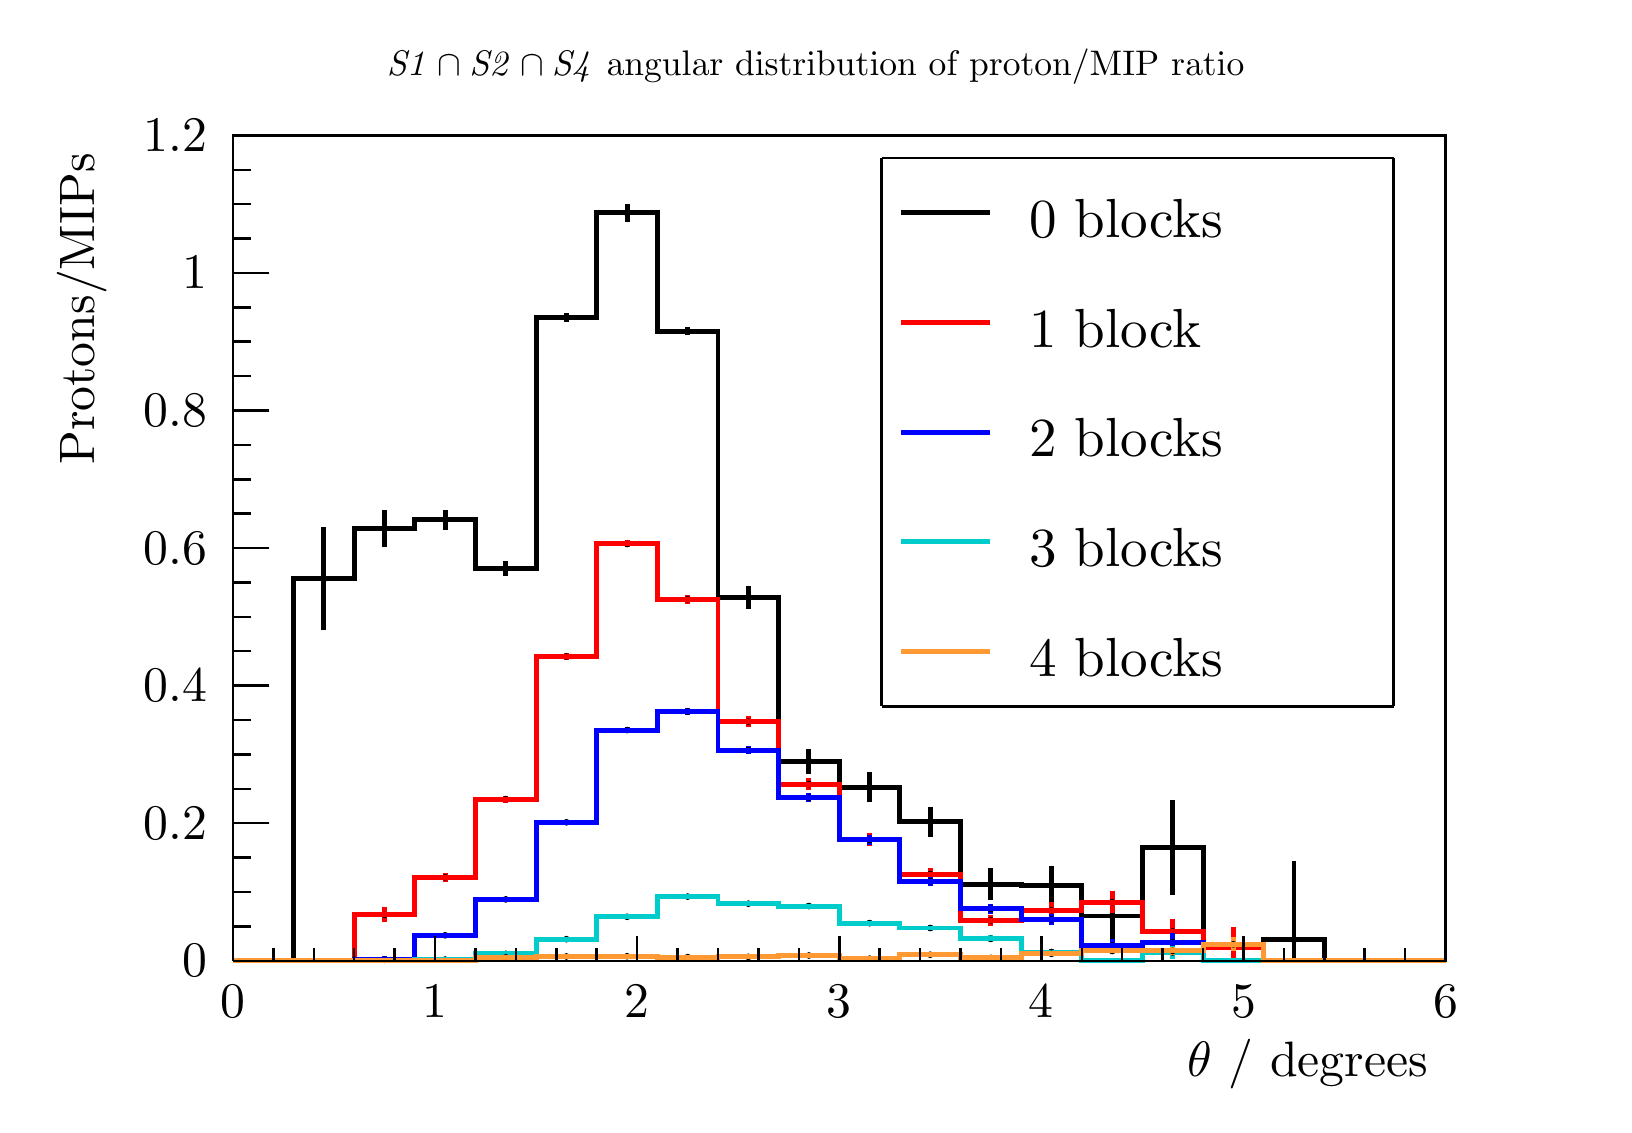
\begin{tikzpicture}
\pgfdeclareplotmark{cross} {
\pgfpathmoveto{\pgfpoint{-0.3\pgfplotmarksize}{\pgfplotmarksize}}
\pgfpathlineto{\pgfpoint{+0.3\pgfplotmarksize}{\pgfplotmarksize}}
\pgfpathlineto{\pgfpoint{+0.3\pgfplotmarksize}{0.3\pgfplotmarksize}}
\pgfpathlineto{\pgfpoint{+1\pgfplotmarksize}{0.3\pgfplotmarksize}}
\pgfpathlineto{\pgfpoint{+1\pgfplotmarksize}{-0.3\pgfplotmarksize}}
\pgfpathlineto{\pgfpoint{+0.3\pgfplotmarksize}{-0.3\pgfplotmarksize}}
\pgfpathlineto{\pgfpoint{+0.3\pgfplotmarksize}{-1.\pgfplotmarksize}}
\pgfpathlineto{\pgfpoint{-0.3\pgfplotmarksize}{-1.\pgfplotmarksize}}
\pgfpathlineto{\pgfpoint{-0.3\pgfplotmarksize}{-0.3\pgfplotmarksize}}
\pgfpathlineto{\pgfpoint{-1.\pgfplotmarksize}{-0.3\pgfplotmarksize}}
\pgfpathlineto{\pgfpoint{-1.\pgfplotmarksize}{0.3\pgfplotmarksize}}
\pgfpathlineto{\pgfpoint{-0.3\pgfplotmarksize}{0.3\pgfplotmarksize}}
\pgfpathclose
\pgfusepathqstroke
}
\pgfdeclareplotmark{cross*} {
\pgfpathmoveto{\pgfpoint{-0.3\pgfplotmarksize}{\pgfplotmarksize}}
\pgfpathlineto{\pgfpoint{+0.3\pgfplotmarksize}{\pgfplotmarksize}}
\pgfpathlineto{\pgfpoint{+0.3\pgfplotmarksize}{0.3\pgfplotmarksize}}
\pgfpathlineto{\pgfpoint{+1\pgfplotmarksize}{0.3\pgfplotmarksize}}
\pgfpathlineto{\pgfpoint{+1\pgfplotmarksize}{-0.3\pgfplotmarksize}}
\pgfpathlineto{\pgfpoint{+0.3\pgfplotmarksize}{-0.3\pgfplotmarksize}}
\pgfpathlineto{\pgfpoint{+0.3\pgfplotmarksize}{-1.\pgfplotmarksize}}
\pgfpathlineto{\pgfpoint{-0.3\pgfplotmarksize}{-1.\pgfplotmarksize}}
\pgfpathlineto{\pgfpoint{-0.3\pgfplotmarksize}{-0.3\pgfplotmarksize}}
\pgfpathlineto{\pgfpoint{-1.\pgfplotmarksize}{-0.3\pgfplotmarksize}}
\pgfpathlineto{\pgfpoint{-1.\pgfplotmarksize}{0.3\pgfplotmarksize}}
\pgfpathlineto{\pgfpoint{-0.3\pgfplotmarksize}{0.3\pgfplotmarksize}}
\pgfpathclose
\pgfusepathqfillstroke
}
\pgfdeclareplotmark{newstar} {
\pgfpathmoveto{\pgfqpoint{0pt}{\pgfplotmarksize}}
\pgfpathlineto{\pgfqpointpolar{44}{0.5\pgfplotmarksize}}
\pgfpathlineto{\pgfqpointpolar{18}{\pgfplotmarksize}}
\pgfpathlineto{\pgfqpointpolar{-20}{0.5\pgfplotmarksize}}
\pgfpathlineto{\pgfqpointpolar{-54}{\pgfplotmarksize}}
\pgfpathlineto{\pgfqpointpolar{-90}{0.5\pgfplotmarksize}}
\pgfpathlineto{\pgfqpointpolar{234}{\pgfplotmarksize}}
\pgfpathlineto{\pgfqpointpolar{198}{0.5\pgfplotmarksize}}
\pgfpathlineto{\pgfqpointpolar{162}{\pgfplotmarksize}}
\pgfpathlineto{\pgfqpointpolar{134}{0.5\pgfplotmarksize}}
\pgfpathclose
\pgfusepathqstroke
}
\pgfdeclareplotmark{newstar*} {
\pgfpathmoveto{\pgfqpoint{0pt}{\pgfplotmarksize}}
\pgfpathlineto{\pgfqpointpolar{44}{0.5\pgfplotmarksize}}
\pgfpathlineto{\pgfqpointpolar{18}{\pgfplotmarksize}}
\pgfpathlineto{\pgfqpointpolar{-20}{0.5\pgfplotmarksize}}
\pgfpathlineto{\pgfqpointpolar{-54}{\pgfplotmarksize}}
\pgfpathlineto{\pgfqpointpolar{-90}{0.5\pgfplotmarksize}}
\pgfpathlineto{\pgfqpointpolar{234}{\pgfplotmarksize}}
\pgfpathlineto{\pgfqpointpolar{198}{0.5\pgfplotmarksize}}
\pgfpathlineto{\pgfqpointpolar{162}{\pgfplotmarksize}}
\pgfpathlineto{\pgfqpointpolar{134}{0.5\pgfplotmarksize}}
\pgfpathclose
\pgfusepathqfillstroke
}
\definecolor{c}{rgb}{1,1,1};
\draw [color=c, fill=c] (0,0) rectangle (20,13.6127);
\draw [color=c, fill=c] (2.6,1.76965) rectangle (18,12.2514);
\definecolor{c}{rgb}{0,0,0};
\draw [c,line width=0.9] (2.6,1.76965) -- (2.6,12.2514) -- (18,12.2514) -- (18,1.76965) -- (2.6,1.76965);
\definecolor{c}{rgb}{1,1,1};
\draw [color=c, fill=c] (2.6,1.76965) rectangle (18,12.2514);
\definecolor{c}{rgb}{0,0,0};
\draw [c,line width=0.9] (2.6,1.76965) -- (2.6,12.2514) -- (18,12.2514) -- (18,1.76965) -- (2.6,1.76965);
\definecolor{c}{rgb}{0,0,0.6};
\draw [c,line width=0.9] (2.6,1.76965) -- (3.37,1.76965) -- (3.37,1.76965) -- (4.14,1.76965) -- (4.14,1.76965) -- (4.91,1.76965) -- (4.91,1.76965) -- (5.68,1.76965) -- (5.68,1.76965) -- (6.45,1.76965) -- (6.45,1.76965) -- (7.22,1.76965) --
 (7.22,1.76965) -- (7.99,1.76965) -- (7.99,1.76965) -- (8.76,1.76965) -- (8.76,1.76965) -- (9.53,1.76965) -- (9.53,1.76965) -- (10.3,1.76965) -- (10.3,1.76965) -- (11.07,1.76965) -- (11.07,1.76965) -- (11.84,1.76965) -- (11.84,1.76965) --
 (12.61,1.76965) -- (12.61,1.76965) -- (13.38,1.76965) -- (13.38,1.76965) -- (14.15,1.76965) -- (14.15,1.76965) -- (14.92,1.76965) -- (14.92,1.76965) -- (15.69,1.76965) -- (15.69,1.76965) -- (16.46,1.76965) -- (16.46,1.76965) -- (17.23,1.76965) --
 (17.23,1.76965) -- (18,1.76965);
\definecolor{c}{rgb}{0,0,0};
\draw [c,line width=0.9] (2.6,1.76965) -- (18,1.76965);
\draw [c,line width=0.9] (2.6,2.08411) -- (2.6,1.76965);
\draw [c,line width=0.9] (3.11333,1.92688) -- (3.11333,1.76965);
\draw [c,line width=0.9] (3.62667,1.92688) -- (3.62667,1.76965);
\draw [c,line width=0.9] (4.14,1.92688) -- (4.14,1.76965);
\draw [c,line width=0.9] (4.65333,1.92688) -- (4.65333,1.76965);
\draw [c,line width=0.9] (5.16667,2.08411) -- (5.16667,1.76965);
\draw [c,line width=0.9] (5.68,1.92688) -- (5.68,1.76965);
\draw [c,line width=0.9] (6.19333,1.92688) -- (6.19333,1.76965);
\draw [c,line width=0.9] (6.70667,1.92688) -- (6.70667,1.76965);
\draw [c,line width=0.9] (7.22,1.92688) -- (7.22,1.76965);
\draw [c,line width=0.9] (7.73333,2.08411) -- (7.73333,1.76965);
\draw [c,line width=0.9] (8.24667,1.92688) -- (8.24667,1.76965);
\draw [c,line width=0.9] (8.76,1.92688) -- (8.76,1.76965);
\draw [c,line width=0.9] (9.27333,1.92688) -- (9.27333,1.76965);
\draw [c,line width=0.9] (9.78667,1.92688) -- (9.78667,1.76965);
\draw [c,line width=0.9] (10.3,2.08411) -- (10.3,1.76965);
\draw [c,line width=0.9] (10.8133,1.92688) -- (10.8133,1.76965);
\draw [c,line width=0.9] (11.3267,1.92688) -- (11.3267,1.76965);
\draw [c,line width=0.9] (11.84,1.92688) -- (11.84,1.76965);
\draw [c,line width=0.9] (12.3533,1.92688) -- (12.3533,1.76965);
\draw [c,line width=0.9] (12.8667,2.08411) -- (12.8667,1.76965);
\draw [c,line width=0.9] (13.38,1.92688) -- (13.38,1.76965);
\draw [c,line width=0.9] (13.8933,1.92688) -- (13.8933,1.76965);
\draw [c,line width=0.9] (14.4067,1.92688) -- (14.4067,1.76965);
\draw [c,line width=0.9] (14.92,1.92688) -- (14.92,1.76965);
\draw [c,line width=0.9] (15.4333,2.08411) -- (15.4333,1.76965);
\draw [c,line width=0.9] (15.9467,1.92688) -- (15.9467,1.76965);
\draw [c,line width=0.9] (16.46,1.92688) -- (16.46,1.76965);
\draw [c,line width=0.9] (16.9733,1.92688) -- (16.9733,1.76965);
\draw [c,line width=0.9] (17.4867,1.92688) -- (17.4867,1.76965);
\draw [c,line width=0.9] (18,2.08411) -- (18,1.76965);
\draw [anchor=base] (2.6,1.04818) node[scale=1.79732, color=c, rotate=0]{0};
\draw [anchor=base] (5.16667,1.04818) node[scale=1.79732, color=c, rotate=0]{1};
\draw [anchor=base] (7.73333,1.04818) node[scale=1.79732, color=c, rotate=0]{2};
\draw [anchor=base] (10.3,1.04818) node[scale=1.79732, color=c, rotate=0]{3};
\draw [anchor=base] (12.8667,1.04818) node[scale=1.79732, color=c, rotate=0]{4};
\draw [anchor=base] (15.4333,1.04818) node[scale=1.79732, color=c, rotate=0]{5};
\draw [anchor=base] (18,1.04818) node[scale=1.79732, color=c, rotate=0]{6};
\draw [anchor= east] (18,0.462832) node[scale=1.79732, color=c, rotate=0]{$\theta$ / degrees};
\draw [c,line width=0.9] (2.6,1.76965) -- (2.6,12.2514);
\draw [c,line width=0.9] (3.062,1.76965) -- (2.6,1.76965);
\draw [c,line width=0.9] (2.831,2.20639) -- (2.6,2.20639);
\draw [c,line width=0.9] (2.831,2.64314) -- (2.6,2.64314);
\draw [c,line width=0.9] (2.831,3.07988) -- (2.6,3.07988);
\draw [c,line width=0.9] (3.062,3.51662) -- (2.6,3.51662);
\draw [c,line width=0.9] (2.831,3.95336) -- (2.6,3.95336);
\draw [c,line width=0.9] (2.831,4.3901) -- (2.6,4.3901);
\draw [c,line width=0.9] (2.831,4.82684) -- (2.6,4.82684);
\draw [c,line width=0.9] (3.062,5.26358) -- (2.6,5.26358);
\draw [c,line width=0.9] (2.831,5.70033) -- (2.6,5.70033);
\draw [c,line width=0.9] (2.831,6.13707) -- (2.6,6.13707);
\draw [c,line width=0.9] (2.831,6.57381) -- (2.6,6.57381);
\draw [c,line width=0.9] (3.062,7.01055) -- (2.6,7.01055);
\draw [c,line width=0.9] (2.831,7.44729) -- (2.6,7.44729);
\draw [c,line width=0.9] (2.831,7.88403) -- (2.6,7.88403);
\draw [c,line width=0.9] (2.831,8.32077) -- (2.6,8.32077);
\draw [c,line width=0.9] (3.062,8.75751) -- (2.6,8.75751);
\draw [c,line width=0.9] (2.831,9.19426) -- (2.6,9.19426);
\draw [c,line width=0.9] (2.831,9.631) -- (2.6,9.631);
\draw [c,line width=0.9] (2.831,10.0677) -- (2.6,10.0677);
\draw [c,line width=0.9] (3.062,10.5045) -- (2.6,10.5045);
\draw [c,line width=0.9] (2.831,10.9412) -- (2.6,10.9412);
\draw [c,line width=0.9] (2.831,11.378) -- (2.6,11.378);
\draw [c,line width=0.9] (2.831,11.8147) -- (2.6,11.8147);
\draw [c,line width=0.9] (3.062,12.2514) -- (2.6,12.2514);
\draw [c,line width=0.9] (3.062,12.2514) -- (2.6,12.2514);
\draw [anchor= east] (2.5,1.76965) node[scale=1.79732, color=c, rotate=0]{0};
\draw [anchor= east] (2.5,3.51662) node[scale=1.79732, color=c, rotate=0]{0.2};
\draw [anchor= east] (2.5,5.26358) node[scale=1.79732, color=c, rotate=0]{0.4};
\draw [anchor= east] (2.5,7.01055) node[scale=1.79732, color=c, rotate=0]{0.6};
\draw [anchor= east] (2.5,8.75751) node[scale=1.79732, color=c, rotate=0]{0.8};
\draw [anchor= east] (2.5,10.5045) node[scale=1.79732, color=c, rotate=0]{1};
\draw [anchor= east] (2.5,12.2514) node[scale=1.79732, color=c, rotate=0]{1.2};
\draw [anchor= east] (0.68,12.2514) node[scale=1.79732, color=c, rotate=90]{ Protons/MIPs};
\draw [c,line width=1.8] (3.755,5.96552) -- (3.755,6.61918);
\draw [c,line width=1.8] (3.755,6.61918) -- (3.755,7.27284);
\foreach \P in {(3.755,6.61918)}{\draw[mark options={color=c,fill=c},mark size=2.402402pt,mark=*,mark size=1pt] plot coordinates {\P};}
\draw [c,line width=1.8] (4.525,7.02017) -- (4.525,7.25485);
\draw [c,line width=1.8] (4.525,7.25485) -- (4.525,7.48953);
\foreach \P in {(4.525,7.25485)}{\draw[mark options={color=c,fill=c},mark size=2.402402pt,mark=*,mark size=1pt] plot coordinates {\P};}
\draw [c,line width=1.8] (5.295,7.24454) -- (5.295,7.36993);
\draw [c,line width=1.8] (5.295,7.36993) -- (5.295,7.49531);
\foreach \P in {(5.295,7.36993)}{\draw[mark options={color=c,fill=c},mark size=2.402402pt,mark=*,mark size=1pt] plot coordinates {\P};}
\draw [c,line width=1.8] (6.065,6.65801) -- (6.065,6.75329);
\draw [c,line width=1.8] (6.065,6.75329) -- (6.065,6.84857);
\foreach \P in {(6.065,6.75329)}{\draw[mark options={color=c,fill=c},mark size=2.402402pt,mark=*,mark size=1pt] plot coordinates {\P};}
\draw [c,line width=1.8] (6.835,9.88682) -- (6.835,9.94428);
\draw [c,line width=1.8] (6.835,9.94428) -- (6.835,10.0017);
\foreach \P in {(6.835,9.94428)}{\draw[mark options={color=c,fill=c},mark size=2.402402pt,mark=*,mark size=1pt] plot coordinates {\P};}
\draw [c,line width=1.8] (7.605,11.157) -- (7.605,11.267);
\draw [c,line width=1.8] (7.605,11.267) -- (7.605,11.3769);
\foreach \P in {(7.605,11.267)}{\draw[mark options={color=c,fill=c},mark size=2.402402pt,mark=*,mark size=1pt] plot coordinates {\P};}
\draw [c,line width=1.8] (8.375,9.71118) -- (8.375,9.76656);
\draw [c,line width=1.8] (8.375,9.76656) -- (8.375,9.82195);
\foreach \P in {(8.375,9.76656)}{\draw[mark options={color=c,fill=c},mark size=2.402402pt,mark=*,mark size=1pt] plot coordinates {\P};}
\draw [c,line width=1.8] (9.145,6.23982) -- (9.145,6.3858);
\draw [c,line width=1.8] (9.145,6.3858) -- (9.145,6.53178);
\foreach \P in {(9.145,6.3858)}{\draw[mark options={color=c,fill=c},mark size=2.402402pt,mark=*,mark size=1pt] plot coordinates {\P};}
\draw [c,line width=1.8] (9.915,4.14538) -- (9.915,4.30397);
\draw [c,line width=1.8] (9.915,4.30397) -- (9.915,4.46257);
\foreach \P in {(9.915,4.30397)}{\draw[mark options={color=c,fill=c},mark size=2.402402pt,mark=*,mark size=1pt] plot coordinates {\P};}
\draw [c,line width=1.8] (10.685,3.78343) -- (10.685,3.9732);
\draw [c,line width=1.8] (10.685,3.9732) -- (10.685,4.16297);
\foreach \P in {(10.685,3.9732)}{\draw[mark options={color=c,fill=c},mark size=2.402402pt,mark=*,mark size=1pt] plot coordinates {\P};}
\draw [c,line width=1.8] (11.455,3.3397) -- (11.455,3.53224);
\draw [c,line width=1.8] (11.455,3.53224) -- (11.455,3.72478);
\foreach \P in {(11.455,3.53224)}{\draw[mark options={color=c,fill=c},mark size=2.402402pt,mark=*,mark size=1pt] plot coordinates {\P};}
\draw [c,line width=1.8] (12.225,2.53805) -- (12.225,2.74072);
\draw [c,line width=1.8] (12.225,2.74072) -- (12.225,2.94338);
\foreach \P in {(12.225,2.74072)}{\draw[mark options={color=c,fill=c},mark size=2.402402pt,mark=*,mark size=1pt] plot coordinates {\P};}
\draw [c,line width=1.8] (12.995,2.48276) -- (12.995,2.72628);
\draw [c,line width=1.8] (12.995,2.72628) -- (12.995,2.9698);
\foreach \P in {(12.995,2.72628)}{\draw[mark options={color=c,fill=c},mark size=2.402402pt,mark=*,mark size=1pt] plot coordinates {\P};}
\draw [c,line width=1.8] (13.765,2.01881) -- (13.765,2.3379);
\draw [c,line width=1.8] (13.765,2.3379) -- (13.765,2.65699);
\foreach \P in {(13.765,2.3379)}{\draw[mark options={color=c,fill=c},mark size=2.402402pt,mark=*,mark size=1pt] plot coordinates {\P};}
\draw [c,line width=1.8] (14.535,2.60709) -- (14.535,3.20937);
\draw [c,line width=1.8] (14.535,3.20937) -- (14.535,3.81165);
\foreach \P in {(14.535,3.20937)}{\draw[mark options={color=c,fill=c},mark size=2.402402pt,mark=*,mark size=1pt] plot coordinates {\P};}
\draw [c,line width=1.8] (16.075,1.76965) -- (16.075,2.03461);
\draw [c,line width=1.8] (16.075,2.03461) -- (16.075,3.04084);
\foreach \P in {(16.075,2.03461)}{\draw[mark options={color=c,fill=c},mark size=2.402402pt,mark=*,mark size=1pt] plot coordinates {\P};}
\draw [c,line width=1.8] (2.6,1.76965) -- (3.37,1.76965) -- (3.37,6.61918) -- (4.14,6.61918) -- (4.14,7.25485) -- (4.91,7.25485) -- (4.91,7.36993) -- (5.68,7.36993) -- (5.68,6.75329) -- (6.45,6.75329) -- (6.45,9.94428) -- (7.22,9.94428) --
 (7.22,11.267) -- (7.99,11.267) -- (7.99,9.76656) -- (8.76,9.76656) -- (8.76,6.3858) -- (9.53,6.3858) -- (9.53,4.30397) -- (10.3,4.30397) -- (10.3,3.9732) -- (11.07,3.9732) -- (11.07,3.53224) -- (11.84,3.53224) -- (11.84,2.74072) -- (12.61,2.74072)
 -- (12.61,2.72628) -- (13.38,2.72628) -- (13.38,2.3379) -- (14.15,2.3379) -- (14.15,3.20937) -- (14.92,3.20937) -- (14.92,1.76965) -- (15.69,1.76965) -- (15.69,2.03461) -- (16.46,2.03461) -- (16.46,1.76965) -- (17.23,1.76965) -- (17.23,1.76965) --
 (18,1.76965);
\definecolor{c}{rgb}{1,0,0};
\draw [c,line width=1.8] (4.525,2.25718) -- (4.525,2.35159);
\draw [c,line width=1.8] (4.525,2.35159) -- (4.525,2.446);
\definecolor{c}{rgb}{0,0,0};
\foreach \P in {(4.525,2.35159)}{\draw[mark options={color=c,fill=c},mark size=2.402402pt,mark=*,mark size=1pt] plot coordinates {\P};}
\definecolor{c}{rgb}{1,0,0};
\draw [c,line width=1.8] (5.295,2.77091) -- (5.295,2.82905);
\draw [c,line width=1.8] (5.295,2.82905) -- (5.295,2.88719);
\definecolor{c}{rgb}{0,0,0};
\foreach \P in {(5.295,2.82905)}{\draw[mark options={color=c,fill=c},mark size=2.402402pt,mark=*,mark size=1pt] plot coordinates {\P};}
\definecolor{c}{rgb}{1,0,0};
\draw [c,line width=1.8] (6.065,3.77647) -- (6.065,3.82233);
\draw [c,line width=1.8] (6.065,3.82233) -- (6.065,3.86819);
\definecolor{c}{rgb}{0,0,0};
\foreach \P in {(6.065,3.82233)}{\draw[mark options={color=c,fill=c},mark size=2.402402pt,mark=*,mark size=1pt] plot coordinates {\P};}
\definecolor{c}{rgb}{1,0,0};
\draw [c,line width=1.8] (6.835,5.59037) -- (6.835,5.63438);
\draw [c,line width=1.8] (6.835,5.63438) -- (6.835,5.67838);
\definecolor{c}{rgb}{0,0,0};
\foreach \P in {(6.835,5.63438)}{\draw[mark options={color=c,fill=c},mark size=2.402402pt,mark=*,mark size=1pt] plot coordinates {\P};}
\definecolor{c}{rgb}{1,0,0};
\draw [c,line width=1.8] (7.605,7.01849) -- (7.605,7.06322);
\draw [c,line width=1.8] (7.605,7.06322) -- (7.605,7.10796);
\definecolor{c}{rgb}{0,0,0};
\foreach \P in {(7.605,7.06322)}{\draw[mark options={color=c,fill=c},mark size=2.402402pt,mark=*,mark size=1pt] plot coordinates {\P};}
\definecolor{c}{rgb}{1,0,0};
\draw [c,line width=1.8] (8.375,6.30504) -- (8.375,6.36061);
\draw [c,line width=1.8] (8.375,6.36061) -- (8.375,6.41618);
\definecolor{c}{rgb}{0,0,0};
\foreach \P in {(8.375,6.36061)}{\draw[mark options={color=c,fill=c},mark size=2.402402pt,mark=*,mark size=1pt] plot coordinates {\P};}
\definecolor{c}{rgb}{1,0,0};
\draw [c,line width=1.8] (9.145,4.73795) -- (9.145,4.80704);
\draw [c,line width=1.8] (9.145,4.80704) -- (9.145,4.87612);
\definecolor{c}{rgb}{0,0,0};
\foreach \P in {(9.145,4.80704)}{\draw[mark options={color=c,fill=c},mark size=2.402402pt,mark=*,mark size=1pt] plot coordinates {\P};}
\definecolor{c}{rgb}{1,0,0};
\draw [c,line width=1.8] (9.915,3.93827) -- (9.915,4.01338);
\draw [c,line width=1.8] (9.915,4.01338) -- (9.915,4.08848);
\definecolor{c}{rgb}{0,0,0};
\foreach \P in {(9.915,4.01338)}{\draw[mark options={color=c,fill=c},mark size=2.402402pt,mark=*,mark size=1pt] plot coordinates {\P};}
\definecolor{c}{rgb}{1,0,0};
\draw [c,line width=1.8] (10.685,3.22568) -- (10.685,3.30686);
\draw [c,line width=1.8] (10.685,3.30686) -- (10.685,3.38804);
\definecolor{c}{rgb}{0,0,0};
\foreach \P in {(10.685,3.30686)}{\draw[mark options={color=c,fill=c},mark size=2.402402pt,mark=*,mark size=1pt] plot coordinates {\P};}
\definecolor{c}{rgb}{1,0,0};
\draw [c,line width=1.8] (11.455,2.78746) -- (11.455,2.87067);
\draw [c,line width=1.8] (11.455,2.87067) -- (11.455,2.95388);
\definecolor{c}{rgb}{0,0,0};
\foreach \P in {(11.455,2.87067)}{\draw[mark options={color=c,fill=c},mark size=2.402402pt,mark=*,mark size=1pt] plot coordinates {\P};}
\definecolor{c}{rgb}{1,0,0};
\draw [c,line width=1.8] (12.225,2.21253) -- (12.225,2.28363);
\draw [c,line width=1.8] (12.225,2.28363) -- (12.225,2.35473);
\definecolor{c}{rgb}{0,0,0};
\foreach \P in {(12.225,2.28363)}{\draw[mark options={color=c,fill=c},mark size=2.402402pt,mark=*,mark size=1pt] plot coordinates {\P};}
\definecolor{c}{rgb}{1,0,0};
\draw [c,line width=1.8] (12.995,2.30897) -- (12.995,2.41012);
\draw [c,line width=1.8] (12.995,2.41012) -- (12.995,2.51127);
\definecolor{c}{rgb}{0,0,0};
\foreach \P in {(12.995,2.41012)}{\draw[mark options={color=c,fill=c},mark size=2.402402pt,mark=*,mark size=1pt] plot coordinates {\P};}
\definecolor{c}{rgb}{1,0,0};
\draw [c,line width=1.8] (13.765,2.37186) -- (13.765,2.51465);
\draw [c,line width=1.8] (13.765,2.51465) -- (13.765,2.65744);
\definecolor{c}{rgb}{0,0,0};
\foreach \P in {(13.765,2.51465)}{\draw[mark options={color=c,fill=c},mark size=2.402402pt,mark=*,mark size=1pt] plot coordinates {\P};}
\definecolor{c}{rgb}{1,0,0};
\draw [c,line width=1.8] (14.535,1.98578) -- (14.535,2.14154);
\draw [c,line width=1.8] (14.535,2.14154) -- (14.535,2.29731);
\definecolor{c}{rgb}{0,0,0};
\foreach \P in {(14.535,2.14154)}{\draw[mark options={color=c,fill=c},mark size=2.402402pt,mark=*,mark size=1pt] plot coordinates {\P};}
\definecolor{c}{rgb}{1,0,0};
\draw [c,line width=1.8] (15.305,1.76965) -- (15.305,1.94371);
\draw [c,line width=1.8] (15.305,1.94371) -- (15.305,2.19744);
\definecolor{c}{rgb}{0,0,0};
\foreach \P in {(15.305,1.94371)}{\draw[mark options={color=c,fill=c},mark size=2.402402pt,mark=*,mark size=1pt] plot coordinates {\P};}
\definecolor{c}{rgb}{1,0,0};
\draw [c,line width=1.8] (2.6,1.76965) -- (3.37,1.76965) -- (3.37,1.76965) -- (4.14,1.76965) -- (4.14,2.35159) -- (4.91,2.35159) -- (4.91,2.82905) -- (5.68,2.82905) -- (5.68,3.82233) -- (6.45,3.82233) -- (6.45,5.63438) -- (7.22,5.63438) --
 (7.22,7.06322) -- (7.99,7.06322) -- (7.99,6.36061) -- (8.76,6.36061) -- (8.76,4.80704) -- (9.53,4.80704) -- (9.53,4.01338) -- (10.3,4.01338) -- (10.3,3.30686) -- (11.07,3.30686) -- (11.07,2.87067) -- (11.84,2.87067) -- (11.84,2.28363) --
 (12.61,2.28363) -- (12.61,2.41012) -- (13.38,2.41012) -- (13.38,2.51465) -- (14.15,2.51465) -- (14.15,2.14154) -- (14.92,2.14154) -- (14.92,1.94371) -- (15.69,1.94371) -- (15.69,1.76965) -- (16.46,1.76965) -- (16.46,1.76965) -- (17.23,1.76965) --
 (17.23,1.76965) -- (18,1.76965);
\definecolor{c}{rgb}{0,0,1};
\draw [c,line width=1.8] (4.525,1.76965) -- (4.525,1.7823);
\draw [c,line width=1.8] (4.525,1.7823) -- (4.525,1.83564);
\definecolor{c}{rgb}{0,0,0};
\foreach \P in {(4.525,1.7823)}{\draw[mark options={color=c,fill=c},mark size=2.402402pt,mark=*,mark size=1pt] plot coordinates {\P};}
\definecolor{c}{rgb}{0,0,1};
\draw [c,line width=1.8] (5.295,2.06026) -- (5.295,2.09298);
\draw [c,line width=1.8] (5.295,2.09298) -- (5.295,2.12571);
\definecolor{c}{rgb}{0,0,0};
\foreach \P in {(5.295,2.09298)}{\draw[mark options={color=c,fill=c},mark size=2.402402pt,mark=*,mark size=1pt] plot coordinates {\P};}
\definecolor{c}{rgb}{0,0,1};
\draw [c,line width=1.8] (6.065,2.5215) -- (6.065,2.54923);
\draw [c,line width=1.8] (6.065,2.54923) -- (6.065,2.57695);
\definecolor{c}{rgb}{0,0,0};
\foreach \P in {(6.065,2.54923)}{\draw[mark options={color=c,fill=c},mark size=2.402402pt,mark=*,mark size=1pt] plot coordinates {\P};}
\definecolor{c}{rgb}{0,0,1};
\draw [c,line width=1.8] (6.835,3.49681) -- (6.835,3.52792);
\draw [c,line width=1.8] (6.835,3.52792) -- (6.835,3.55903);
\definecolor{c}{rgb}{0,0,0};
\foreach \P in {(6.835,3.52792)}{\draw[mark options={color=c,fill=c},mark size=2.402402pt,mark=*,mark size=1pt] plot coordinates {\P};}
\definecolor{c}{rgb}{0,0,1};
\draw [c,line width=1.8] (7.605,4.66274) -- (7.605,4.69928);
\draw [c,line width=1.8] (7.605,4.69928) -- (7.605,4.73582);
\definecolor{c}{rgb}{0,0,0};
\foreach \P in {(7.605,4.69928)}{\draw[mark options={color=c,fill=c},mark size=2.402402pt,mark=*,mark size=1pt] plot coordinates {\P};}
\definecolor{c}{rgb}{0,0,1};
\draw [c,line width=1.8] (8.375,4.89186) -- (8.375,4.93533);
\draw [c,line width=1.8] (8.375,4.93533) -- (8.375,4.9788);
\definecolor{c}{rgb}{0,0,0};
\foreach \P in {(8.375,4.93533)}{\draw[mark options={color=c,fill=c},mark size=2.402402pt,mark=*,mark size=1pt] plot coordinates {\P};}
\definecolor{c}{rgb}{0,0,1};
\draw [c,line width=1.8] (9.145,4.39433) -- (9.145,4.44478);
\draw [c,line width=1.8] (9.145,4.44478) -- (9.145,4.49524);
\definecolor{c}{rgb}{0,0,0};
\foreach \P in {(9.145,4.44478)}{\draw[mark options={color=c,fill=c},mark size=2.402402pt,mark=*,mark size=1pt] plot coordinates {\P};}
\definecolor{c}{rgb}{0,0,1};
\draw [c,line width=1.8] (9.915,3.78582) -- (9.915,3.84078);
\draw [c,line width=1.8] (9.915,3.84078) -- (9.915,3.89575);
\definecolor{c}{rgb}{0,0,0};
\foreach \P in {(9.915,3.84078)}{\draw[mark options={color=c,fill=c},mark size=2.402402pt,mark=*,mark size=1pt] plot coordinates {\P};}
\definecolor{c}{rgb}{0,0,1};
\draw [c,line width=1.8] (10.685,3.24461) -- (10.685,3.3036);
\draw [c,line width=1.8] (10.685,3.3036) -- (10.685,3.36259);
\definecolor{c}{rgb}{0,0,0};
\foreach \P in {(10.685,3.3036)}{\draw[mark options={color=c,fill=c},mark size=2.402402pt,mark=*,mark size=1pt] plot coordinates {\P};}
\definecolor{c}{rgb}{0,0,1};
\draw [c,line width=1.8] (11.455,2.72135) -- (11.455,2.77999);
\draw [c,line width=1.8] (11.455,2.77999) -- (11.455,2.83863);
\definecolor{c}{rgb}{0,0,0};
\foreach \P in {(11.455,2.77999)}{\draw[mark options={color=c,fill=c},mark size=2.402402pt,mark=*,mark size=1pt] plot coordinates {\P};}
\definecolor{c}{rgb}{0,0,1};
\draw [c,line width=1.8] (12.225,2.36619) -- (12.225,2.42732);
\draw [c,line width=1.8] (12.225,2.42732) -- (12.225,2.48844);
\definecolor{c}{rgb}{0,0,0};
\foreach \P in {(12.225,2.42732)}{\draw[mark options={color=c,fill=c},mark size=2.402402pt,mark=*,mark size=1pt] plot coordinates {\P};}
\definecolor{c}{rgb}{0,0,1};
\draw [c,line width=1.8] (12.995,2.22581) -- (12.995,2.29456);
\draw [c,line width=1.8] (12.995,2.29456) -- (12.995,2.36332);
\definecolor{c}{rgb}{0,0,0};
\foreach \P in {(12.995,2.29456)}{\draw[mark options={color=c,fill=c},mark size=2.402402pt,mark=*,mark size=1pt] plot coordinates {\P};}
\definecolor{c}{rgb}{0,0,1};
\draw [c,line width=1.8] (13.765,1.88797) -- (13.765,1.96423);
\draw [c,line width=1.8] (13.765,1.96423) -- (13.765,2.04048);
\definecolor{c}{rgb}{0,0,0};
\foreach \P in {(13.765,1.96423)}{\draw[mark options={color=c,fill=c},mark size=2.402402pt,mark=*,mark size=1pt] plot coordinates {\P};}
\definecolor{c}{rgb}{0,0,1};
\draw [c,line width=1.8] (14.535,1.88836) -- (14.535,2.00549);
\draw [c,line width=1.8] (14.535,2.00549) -- (14.535,2.12261);
\definecolor{c}{rgb}{0,0,0};
\foreach \P in {(14.535,2.00549)}{\draw[mark options={color=c,fill=c},mark size=2.402402pt,mark=*,mark size=1pt] plot coordinates {\P};}
\definecolor{c}{rgb}{0,0,1};
\draw [c,line width=1.8] (2.6,1.76965) -- (3.37,1.76965) -- (3.37,1.76965) -- (4.14,1.76965) -- (4.14,1.7823) -- (4.91,1.7823) -- (4.91,2.09298) -- (5.68,2.09298) -- (5.68,2.54923) -- (6.45,2.54923) -- (6.45,3.52792) -- (7.22,3.52792) --
 (7.22,4.69928) -- (7.99,4.69928) -- (7.99,4.93533) -- (8.76,4.93533) -- (8.76,4.44478) -- (9.53,4.44478) -- (9.53,3.84078) -- (10.3,3.84078) -- (10.3,3.3036) -- (11.07,3.3036) -- (11.07,2.77999) -- (11.84,2.77999) -- (11.84,2.42732) --
 (12.61,2.42732) -- (12.61,2.29456) -- (13.38,2.29456) -- (13.38,1.96423) -- (14.15,1.96423) -- (14.15,2.00549) -- (14.92,2.00549) -- (14.92,1.76965) -- (15.69,1.76965) -- (15.69,1.76965) -- (16.46,1.76965) -- (16.46,1.76965) -- (17.23,1.76965) --
 (17.23,1.76965) -- (18,1.76965);
\definecolor{c}{rgb}{0,0.8,0.8};
\draw [c,line width=1.8] (5.295,1.76965) -- (5.295,1.78457);
\draw [c,line width=1.8] (5.295,1.78457) -- (5.295,1.80271);
\definecolor{c}{rgb}{0,0,0};
\foreach \P in {(5.295,1.78457)}{\draw[mark options={color=c,fill=c},mark size=2.402402pt,mark=*,mark size=1pt] plot coordinates {\P};}
\definecolor{c}{rgb}{0,0.8,0.8};
\draw [c,line width=1.8] (6.065,1.8446) -- (6.065,1.8573);
\draw [c,line width=1.8] (6.065,1.8573) -- (6.065,1.87);
\definecolor{c}{rgb}{0,0,0};
\foreach \P in {(6.065,1.8573)}{\draw[mark options={color=c,fill=c},mark size=2.402402pt,mark=*,mark size=1pt] plot coordinates {\P};}
\definecolor{c}{rgb}{0,0.8,0.8};
\draw [c,line width=1.8] (6.835,2.02672) -- (6.835,2.04365);
\draw [c,line width=1.8] (6.835,2.04365) -- (6.835,2.06058);
\definecolor{c}{rgb}{0,0,0};
\foreach \P in {(6.835,2.04365)}{\draw[mark options={color=c,fill=c},mark size=2.402402pt,mark=*,mark size=1pt] plot coordinates {\P};}
\definecolor{c}{rgb}{0,0.8,0.8};
\draw [c,line width=1.8] (7.605,2.30633) -- (7.605,2.32789);
\draw [c,line width=1.8] (7.605,2.32789) -- (7.605,2.34945);
\definecolor{c}{rgb}{0,0,0};
\foreach \P in {(7.605,2.32789)}{\draw[mark options={color=c,fill=c},mark size=2.402402pt,mark=*,mark size=1pt] plot coordinates {\P};}
\definecolor{c}{rgb}{0,0.8,0.8};
\draw [c,line width=1.8] (8.375,2.55536) -- (8.375,2.58455);
\draw [c,line width=1.8] (8.375,2.58455) -- (8.375,2.61374);
\definecolor{c}{rgb}{0,0,0};
\foreach \P in {(8.375,2.58455)}{\draw[mark options={color=c,fill=c},mark size=2.402402pt,mark=*,mark size=1pt] plot coordinates {\P};}
\definecolor{c}{rgb}{0,0.8,0.8};
\draw [c,line width=1.8] (9.145,2.46079) -- (9.145,2.49448);
\draw [c,line width=1.8] (9.145,2.49448) -- (9.145,2.52816);
\definecolor{c}{rgb}{0,0,0};
\foreach \P in {(9.145,2.49448)}{\draw[mark options={color=c,fill=c},mark size=2.402402pt,mark=*,mark size=1pt] plot coordinates {\P};}
\definecolor{c}{rgb}{0,0.8,0.8};
\draw [c,line width=1.8] (9.915,2.42409) -- (9.915,2.46387);
\draw [c,line width=1.8] (9.915,2.46387) -- (9.915,2.50366);
\definecolor{c}{rgb}{0,0,0};
\foreach \P in {(9.915,2.46387)}{\draw[mark options={color=c,fill=c},mark size=2.402402pt,mark=*,mark size=1pt] plot coordinates {\P};}
\definecolor{c}{rgb}{0,0.8,0.8};
\draw [c,line width=1.8] (10.685,2.20946) -- (10.685,2.2468);
\draw [c,line width=1.8] (10.685,2.2468) -- (10.685,2.28414);
\definecolor{c}{rgb}{0,0,0};
\foreach \P in {(10.685,2.2468)}{\draw[mark options={color=c,fill=c},mark size=2.402402pt,mark=*,mark size=1pt] plot coordinates {\P};}
\definecolor{c}{rgb}{0,0.8,0.8};
\draw [c,line width=1.8] (11.455,2.14459) -- (11.455,2.18563);
\draw [c,line width=1.8] (11.455,2.18563) -- (11.455,2.22667);
\definecolor{c}{rgb}{0,0,0};
\foreach \P in {(11.455,2.18563)}{\draw[mark options={color=c,fill=c},mark size=2.402402pt,mark=*,mark size=1pt] plot coordinates {\P};}
\definecolor{c}{rgb}{0,0.8,0.8};
\draw [c,line width=1.8] (12.225,2.00237) -- (12.225,2.0483);
\draw [c,line width=1.8] (12.225,2.0483) -- (12.225,2.09422);
\definecolor{c}{rgb}{0,0,0};
\foreach \P in {(12.225,2.0483)}{\draw[mark options={color=c,fill=c},mark size=2.402402pt,mark=*,mark size=1pt] plot coordinates {\P};}
\definecolor{c}{rgb}{0,0.8,0.8};
\draw [c,line width=1.8] (12.995,1.8366) -- (12.995,1.8805);
\draw [c,line width=1.8] (12.995,1.8805) -- (12.995,1.92441);
\definecolor{c}{rgb}{0,0,0};
\foreach \P in {(12.995,1.8805)}{\draw[mark options={color=c,fill=c},mark size=2.402402pt,mark=*,mark size=1pt] plot coordinates {\P};}
\definecolor{c}{rgb}{0,0.8,0.8};
\draw [c,line width=1.8] (14.535,1.78926) -- (14.535,1.8749);
\draw [c,line width=1.8] (14.535,1.8749) -- (14.535,1.96054);
\definecolor{c}{rgb}{0,0,0};
\foreach \P in {(14.535,1.8749)}{\draw[mark options={color=c,fill=c},mark size=2.402402pt,mark=*,mark size=1pt] plot coordinates {\P};}
\definecolor{c}{rgb}{0,0.8,0.8};
\draw [c,line width=1.8] (2.6,1.76965) -- (3.37,1.76965) -- (3.37,1.76965) -- (4.14,1.76965) -- (4.14,1.76965) -- (4.91,1.76965) -- (4.91,1.78457) -- (5.68,1.78457) -- (5.68,1.8573) -- (6.45,1.8573) -- (6.45,2.04365) -- (7.22,2.04365) --
 (7.22,2.32789) -- (7.99,2.32789) -- (7.99,2.58455) -- (8.76,2.58455) -- (8.76,2.49448) -- (9.53,2.49448) -- (9.53,2.46387) -- (10.3,2.46387) -- (10.3,2.2468) -- (11.07,2.2468) -- (11.07,2.18563) -- (11.84,2.18563) -- (11.84,2.0483) -- (12.61,2.0483)
 -- (12.61,1.8805) -- (13.38,1.8805) -- (13.38,1.76965) -- (14.15,1.76965) -- (14.15,1.8749) -- (14.92,1.8749) -- (14.92,1.76965) -- (15.69,1.76965) -- (15.69,1.76965) -- (16.46,1.76965) -- (16.46,1.76965) -- (17.23,1.76965) -- (17.23,1.76965) --
 (18,1.76965);
\definecolor{c}{rgb}{1,0.6,0.2};
\draw [c,line width=1.8] (6.065,1.8082) -- (6.065,1.81294);
\draw [c,line width=1.8] (6.065,1.81294) -- (6.065,1.81769);
\definecolor{c}{rgb}{0,0,0};
\foreach \P in {(6.065,1.81294)}{\draw[mark options={color=c,fill=c},mark size=2.402402pt,mark=*,mark size=1pt] plot coordinates {\P};}
\definecolor{c}{rgb}{1,0.6,0.2};
\draw [c,line width=1.8] (6.835,1.81861) -- (6.835,1.82418);
\draw [c,line width=1.8] (6.835,1.82418) -- (6.835,1.82974);
\definecolor{c}{rgb}{0,0,0};
\foreach \P in {(6.835,1.82418)}{\draw[mark options={color=c,fill=c},mark size=2.402402pt,mark=*,mark size=1pt] plot coordinates {\P};}
\definecolor{c}{rgb}{1,0.6,0.2};
\draw [c,line width=1.8] (7.605,1.822) -- (7.605,1.82706);
\draw [c,line width=1.8] (7.605,1.82706) -- (7.605,1.83212);
\definecolor{c}{rgb}{0,0,0};
\foreach \P in {(7.605,1.82706)}{\draw[mark options={color=c,fill=c},mark size=2.402402pt,mark=*,mark size=1pt] plot coordinates {\P};}
\definecolor{c}{rgb}{1,0.6,0.2};
\draw [c,line width=1.8] (8.375,1.81073) -- (8.375,1.8155);
\draw [c,line width=1.8] (8.375,1.8155) -- (8.375,1.82027);
\definecolor{c}{rgb}{0,0,0};
\foreach \P in {(8.375,1.8155)}{\draw[mark options={color=c,fill=c},mark size=2.402402pt,mark=*,mark size=1pt] plot coordinates {\P};}
\definecolor{c}{rgb}{1,0.6,0.2};
\draw [c,line width=1.8] (9.145,1.81131) -- (9.145,1.81903);
\draw [c,line width=1.8] (9.145,1.81903) -- (9.145,1.82675);
\definecolor{c}{rgb}{0,0,0};
\foreach \P in {(9.145,1.81903)}{\draw[mark options={color=c,fill=c},mark size=2.402402pt,mark=*,mark size=1pt] plot coordinates {\P};}
\definecolor{c}{rgb}{1,0.6,0.2};
\draw [c,line width=1.8] (9.915,1.82508) -- (9.915,1.83644);
\draw [c,line width=1.8] (9.915,1.83644) -- (9.915,1.8478);
\definecolor{c}{rgb}{0,0,0};
\foreach \P in {(9.915,1.83644)}{\draw[mark options={color=c,fill=c},mark size=2.402402pt,mark=*,mark size=1pt] plot coordinates {\P};}
\definecolor{c}{rgb}{1,0.6,0.2};
\draw [c,line width=1.8] (10.685,1.79053) -- (10.685,1.79625);
\draw [c,line width=1.8] (10.685,1.79625) -- (10.685,1.80197);
\definecolor{c}{rgb}{0,0,0};
\foreach \P in {(10.685,1.79625)}{\draw[mark options={color=c,fill=c},mark size=2.402402pt,mark=*,mark size=1pt] plot coordinates {\P};}
\definecolor{c}{rgb}{1,0.6,0.2};
\draw [c,line width=1.8] (11.455,1.83001) -- (11.455,1.84612);
\draw [c,line width=1.8] (11.455,1.84612) -- (11.455,1.86223);
\definecolor{c}{rgb}{0,0,0};
\foreach \P in {(11.455,1.84612)}{\draw[mark options={color=c,fill=c},mark size=2.402402pt,mark=*,mark size=1pt] plot coordinates {\P};}
\definecolor{c}{rgb}{1,0.6,0.2};
\draw [c,line width=1.8] (12.225,1.78986) -- (12.225,1.80562);
\draw [c,line width=1.8] (12.225,1.80562) -- (12.225,1.82137);
\definecolor{c}{rgb}{0,0,0};
\foreach \P in {(12.225,1.80562)}{\draw[mark options={color=c,fill=c},mark size=2.402402pt,mark=*,mark size=1pt] plot coordinates {\P};}
\definecolor{c}{rgb}{1,0.6,0.2};
\draw [c,line width=1.8] (12.995,1.82889) -- (12.995,1.85773);
\draw [c,line width=1.8] (12.995,1.85773) -- (12.995,1.88657);
\definecolor{c}{rgb}{0,0,0};
\foreach \P in {(12.995,1.85773)}{\draw[mark options={color=c,fill=c},mark size=2.402402pt,mark=*,mark size=1pt] plot coordinates {\P};}
\definecolor{c}{rgb}{1,0.6,0.2};
\draw [c,line width=1.8] (13.765,1.85379) -- (13.765,1.89371);
\draw [c,line width=1.8] (13.765,1.89371) -- (13.765,1.93363);
\definecolor{c}{rgb}{0,0,0};
\foreach \P in {(13.765,1.89371)}{\draw[mark options={color=c,fill=c},mark size=2.402402pt,mark=*,mark size=1pt] plot coordinates {\P};}
\definecolor{c}{rgb}{1,0.6,0.2};
\draw [c,line width=1.8] (14.535,1.84554) -- (14.535,1.89421);
\draw [c,line width=1.8] (14.535,1.89421) -- (14.535,1.94289);
\definecolor{c}{rgb}{0,0,0};
\foreach \P in {(14.535,1.89421)}{\draw[mark options={color=c,fill=c},mark size=2.402402pt,mark=*,mark size=1pt] plot coordinates {\P};}
\definecolor{c}{rgb}{1,0.6,0.2};
\draw [c,line width=1.8] (15.305,1.88744) -- (15.305,1.97804);
\draw [c,line width=1.8] (15.305,1.97804) -- (15.305,2.06865);
\definecolor{c}{rgb}{0,0,0};
\foreach \P in {(15.305,1.97804)}{\draw[mark options={color=c,fill=c},mark size=2.402402pt,mark=*,mark size=1pt] plot coordinates {\P};}
\definecolor{c}{rgb}{1,0.6,0.2};
\draw [c,line width=1.8] (2.6,1.76965) -- (3.37,1.76965) -- (3.37,1.76965) -- (4.14,1.76965) -- (4.14,1.76965) -- (4.91,1.76965) -- (4.91,1.76965) -- (5.68,1.76965) -- (5.68,1.81294) -- (6.45,1.81294) -- (6.45,1.82418) -- (7.22,1.82418) --
 (7.22,1.82706) -- (7.99,1.82706) -- (7.99,1.8155) -- (8.76,1.8155) -- (8.76,1.81903) -- (9.53,1.81903) -- (9.53,1.83644) -- (10.3,1.83644) -- (10.3,1.79625) -- (11.07,1.79625) -- (11.07,1.84612) -- (11.84,1.84612) -- (11.84,1.80562) --
 (12.61,1.80562) -- (12.61,1.85773) -- (13.38,1.85773) -- (13.38,1.89371) -- (14.15,1.89371) -- (14.15,1.89421) -- (14.92,1.89421) -- (14.92,1.97804) -- (15.69,1.97804) -- (15.69,1.76965) -- (16.46,1.76965) -- (16.46,1.76965) -- (17.23,1.76965) --
 (17.23,1.76965) -- (18,1.76965);
\definecolor{c}{rgb}{0,0,0};
\draw [c,line width=0.9] (2.6,1.76965) -- (18,1.76965);
\draw [c,line width=0.9] (2.6,2.08411) -- (2.6,1.76965);
\draw [c,line width=0.9] (3.11333,1.92688) -- (3.11333,1.76965);
\draw [c,line width=0.9] (3.62667,1.92688) -- (3.62667,1.76965);
\draw [c,line width=0.9] (4.14,1.92688) -- (4.14,1.76965);
\draw [c,line width=0.9] (4.65333,1.92688) -- (4.65333,1.76965);
\draw [c,line width=0.9] (5.16667,2.08411) -- (5.16667,1.76965);
\draw [c,line width=0.9] (5.68,1.92688) -- (5.68,1.76965);
\draw [c,line width=0.9] (6.19333,1.92688) -- (6.19333,1.76965);
\draw [c,line width=0.9] (6.70667,1.92688) -- (6.70667,1.76965);
\draw [c,line width=0.9] (7.22,1.92688) -- (7.22,1.76965);
\draw [c,line width=0.9] (7.73333,2.08411) -- (7.73333,1.76965);
\draw [c,line width=0.9] (8.24667,1.92688) -- (8.24667,1.76965);
\draw [c,line width=0.9] (8.76,1.92688) -- (8.76,1.76965);
\draw [c,line width=0.9] (9.27333,1.92688) -- (9.27333,1.76965);
\draw [c,line width=0.9] (9.78667,1.92688) -- (9.78667,1.76965);
\draw [c,line width=0.9] (10.3,2.08411) -- (10.3,1.76965);
\draw [c,line width=0.9] (10.8133,1.92688) -- (10.8133,1.76965);
\draw [c,line width=0.9] (11.3267,1.92688) -- (11.3267,1.76965);
\draw [c,line width=0.9] (11.84,1.92688) -- (11.84,1.76965);
\draw [c,line width=0.9] (12.3533,1.92688) -- (12.3533,1.76965);
\draw [c,line width=0.9] (12.8667,2.08411) -- (12.8667,1.76965);
\draw [c,line width=0.9] (13.38,1.92688) -- (13.38,1.76965);
\draw [c,line width=0.9] (13.8933,1.92688) -- (13.8933,1.76965);
\draw [c,line width=0.9] (14.4067,1.92688) -- (14.4067,1.76965);
\draw [c,line width=0.9] (14.92,1.92688) -- (14.92,1.76965);
\draw [c,line width=0.9] (15.4333,2.08411) -- (15.4333,1.76965);
\draw [c,line width=0.9] (15.9467,1.92688) -- (15.9467,1.76965);
\draw [c,line width=0.9] (16.46,1.92688) -- (16.46,1.76965);
\draw [c,line width=0.9] (16.9733,1.92688) -- (16.9733,1.76965);
\draw [c,line width=0.9] (17.4867,1.92688) -- (17.4867,1.76965);
\draw [c,line width=0.9] (18,2.08411) -- (18,1.76965);
\draw [c,line width=0.9] (2.6,1.76965) -- (2.6,12.2514);
\draw [c,line width=0.9] (3.062,1.76965) -- (2.6,1.76965);
\draw [c,line width=0.9] (2.831,2.20639) -- (2.6,2.20639);
\draw [c,line width=0.9] (2.831,2.64314) -- (2.6,2.64314);
\draw [c,line width=0.9] (2.831,3.07988) -- (2.6,3.07988);
\draw [c,line width=0.9] (3.062,3.51662) -- (2.6,3.51662);
\draw [c,line width=0.9] (2.831,3.95336) -- (2.6,3.95336);
\draw [c,line width=0.9] (2.831,4.3901) -- (2.6,4.3901);
\draw [c,line width=0.9] (2.831,4.82684) -- (2.6,4.82684);
\draw [c,line width=0.9] (3.062,5.26358) -- (2.6,5.26358);
\draw [c,line width=0.9] (2.831,5.70033) -- (2.6,5.70033);
\draw [c,line width=0.9] (2.831,6.13707) -- (2.6,6.13707);
\draw [c,line width=0.9] (2.831,6.57381) -- (2.6,6.57381);
\draw [c,line width=0.9] (3.062,7.01055) -- (2.6,7.01055);
\draw [c,line width=0.9] (2.831,7.44729) -- (2.6,7.44729);
\draw [c,line width=0.9] (2.831,7.88403) -- (2.6,7.88403);
\draw [c,line width=0.9] (2.831,8.32077) -- (2.6,8.32077);
\draw [c,line width=0.9] (3.062,8.75751) -- (2.6,8.75751);
\draw [c,line width=0.9] (2.831,9.19426) -- (2.6,9.19426);
\draw [c,line width=0.9] (2.831,9.631) -- (2.6,9.631);
\draw [c,line width=0.9] (2.831,10.0677) -- (2.6,10.0677);
\draw [c,line width=0.9] (3.062,10.5045) -- (2.6,10.5045);
\draw [c,line width=0.9] (2.831,10.9412) -- (2.6,10.9412);
\draw [c,line width=0.9] (2.831,11.378) -- (2.6,11.378);
\draw [c,line width=0.9] (2.831,11.8147) -- (2.6,11.8147);
\draw [c,line width=0.9] (3.062,12.2514) -- (2.6,12.2514);
\draw [c,line width=0.9] (3.062,12.2514) -- (2.6,12.2514);
\draw (10,13.1285) node[scale=1.2838, color=c, rotate=0]{$\mathit{S1} \cap \mathit{S2} \cap \mathit{S4}$ angular distribution of proton/MIP ratio};
\definecolor{c}{rgb}{1,1,1};
\draw [color=c, fill=c] (10.8382,5) rectangle (17.341,11.9653);
\definecolor{c}{rgb}{0,0,0};
\draw [c,line width=0.9] (10.8382,5) -- (17.341,5);
\draw [c,line width=0.9] (17.341,5) -- (17.341,11.9653);
\draw [c,line width=0.9] (17.341,11.9653) -- (10.8382,11.9653);
\draw [c,line width=0.9] (10.8382,11.9653) -- (10.8382,5);
\draw [anchor=base west] (12.4639,10.9553) node[scale=1.98989, color=c, rotate=0]{0 blocks};
\draw [c,line width=1.8] (11.082,11.2688) -- (12.22,11.2688);
\draw [anchor=base west] (12.4639,9.56228) node[scale=1.98989, color=c, rotate=0]{1 block};
\definecolor{c}{rgb}{1,0,0};
\draw [c,line width=1.8] (11.082,9.87572) -- (12.22,9.87572);
\definecolor{c}{rgb}{0,0,0};
\draw [anchor=base west] (12.4639,8.16922) node[scale=1.98989, color=c, rotate=0]{2 blocks};
\definecolor{c}{rgb}{0,0,1};
\draw [c,line width=1.8] (11.082,8.48266) -- (12.22,8.48266);
\definecolor{c}{rgb}{0,0,0};
\draw [anchor=base west] (12.4639,6.77616) node[scale=1.98989, color=c, rotate=0]{3 blocks};
\definecolor{c}{rgb}{0,0.8,0.8};
\draw [c,line width=1.8] (11.082,7.0896) -- (12.22,7.0896);
\definecolor{c}{rgb}{0,0,0};
\draw [anchor=base west] (12.4639,5.38309) node[scale=1.98989, color=c, rotate=0]{4 blocks};
\definecolor{c}{rgb}{1,0.6,0.2};
\draw [c,line width=1.8] (11.082,5.69653) -- (12.22,5.69653);
\end{tikzpicture}

    \end{adjustbox}
  \end{minipage}
  \hspace{0.3cm}
  \begin{minipage}[t]{0.48\textwidth}
    \begin{adjustbox}{max totalsize={\textwidth}{.35\textheight}, center}
      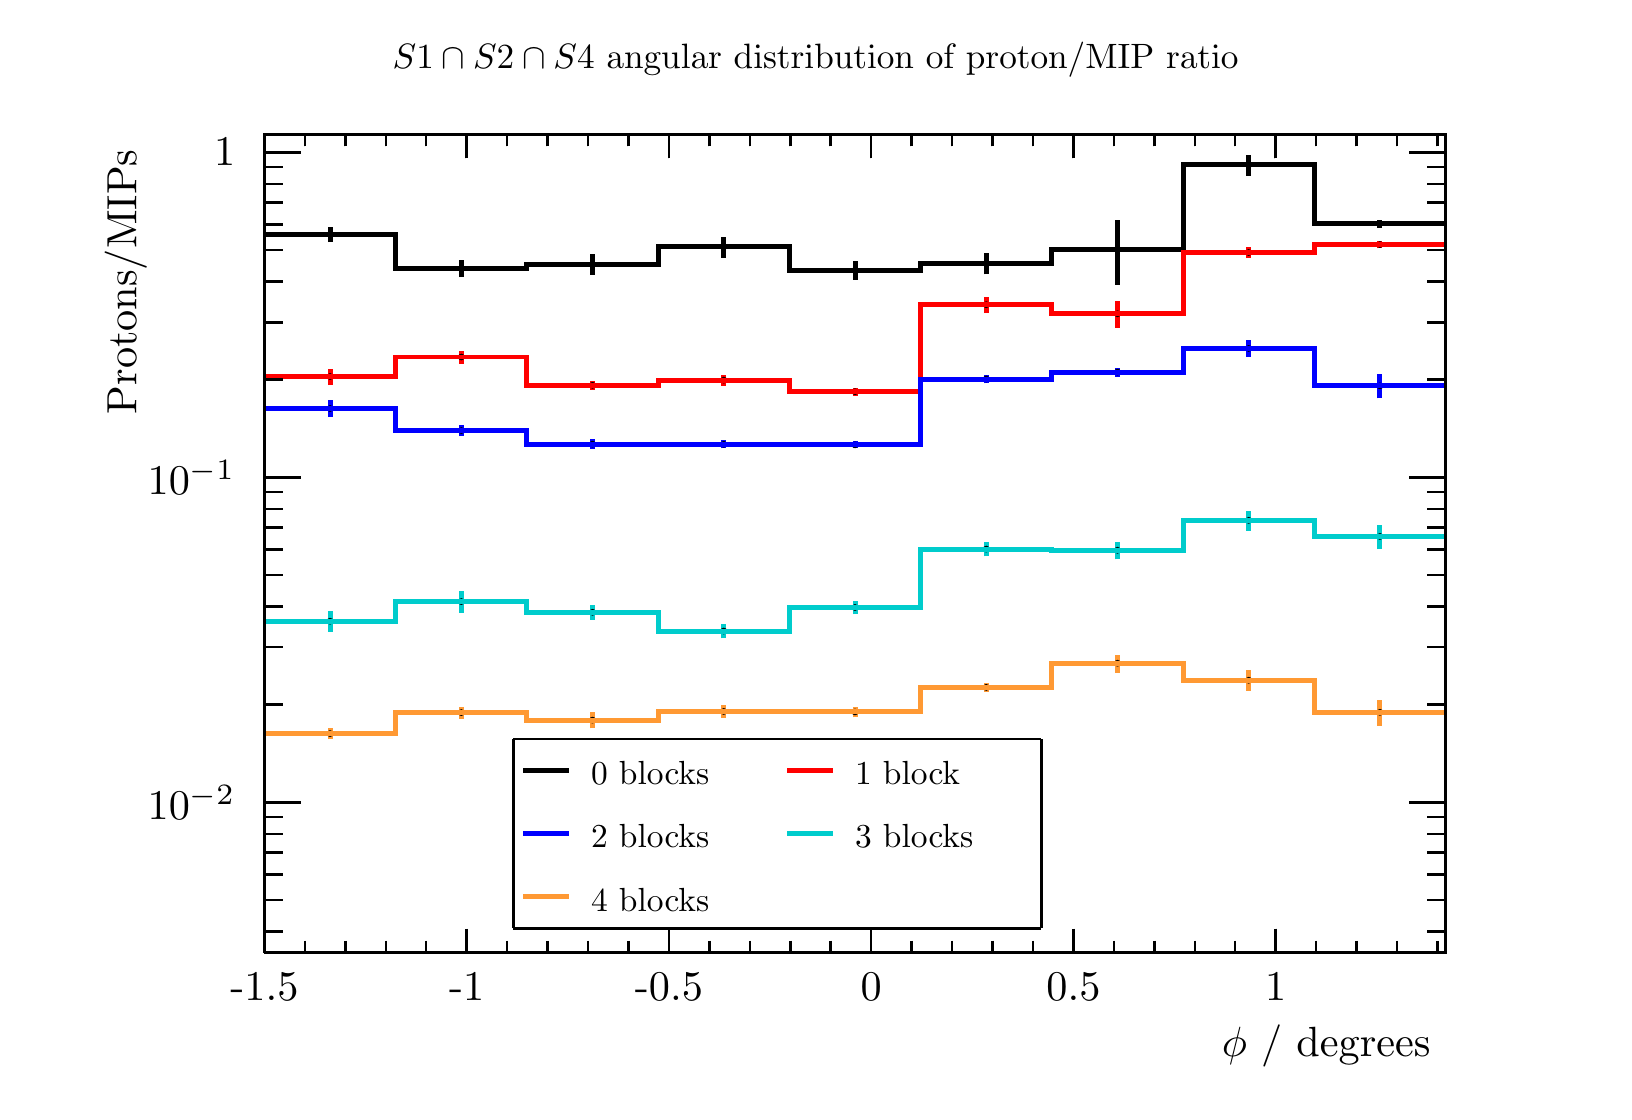
\begin{tikzpicture}
\pgfdeclareplotmark{cross} {
\pgfpathmoveto{\pgfpoint{-0.3\pgfplotmarksize}{\pgfplotmarksize}}
\pgfpathlineto{\pgfpoint{+0.3\pgfplotmarksize}{\pgfplotmarksize}}
\pgfpathlineto{\pgfpoint{+0.3\pgfplotmarksize}{0.3\pgfplotmarksize}}
\pgfpathlineto{\pgfpoint{+1\pgfplotmarksize}{0.3\pgfplotmarksize}}
\pgfpathlineto{\pgfpoint{+1\pgfplotmarksize}{-0.3\pgfplotmarksize}}
\pgfpathlineto{\pgfpoint{+0.3\pgfplotmarksize}{-0.3\pgfplotmarksize}}
\pgfpathlineto{\pgfpoint{+0.3\pgfplotmarksize}{-1.\pgfplotmarksize}}
\pgfpathlineto{\pgfpoint{-0.3\pgfplotmarksize}{-1.\pgfplotmarksize}}
\pgfpathlineto{\pgfpoint{-0.3\pgfplotmarksize}{-0.3\pgfplotmarksize}}
\pgfpathlineto{\pgfpoint{-1.\pgfplotmarksize}{-0.3\pgfplotmarksize}}
\pgfpathlineto{\pgfpoint{-1.\pgfplotmarksize}{0.3\pgfplotmarksize}}
\pgfpathlineto{\pgfpoint{-0.3\pgfplotmarksize}{0.3\pgfplotmarksize}}
\pgfpathclose
\pgfusepathqstroke
}
\pgfdeclareplotmark{cross*} {
\pgfpathmoveto{\pgfpoint{-0.3\pgfplotmarksize}{\pgfplotmarksize}}
\pgfpathlineto{\pgfpoint{+0.3\pgfplotmarksize}{\pgfplotmarksize}}
\pgfpathlineto{\pgfpoint{+0.3\pgfplotmarksize}{0.3\pgfplotmarksize}}
\pgfpathlineto{\pgfpoint{+1\pgfplotmarksize}{0.3\pgfplotmarksize}}
\pgfpathlineto{\pgfpoint{+1\pgfplotmarksize}{-0.3\pgfplotmarksize}}
\pgfpathlineto{\pgfpoint{+0.3\pgfplotmarksize}{-0.3\pgfplotmarksize}}
\pgfpathlineto{\pgfpoint{+0.3\pgfplotmarksize}{-1.\pgfplotmarksize}}
\pgfpathlineto{\pgfpoint{-0.3\pgfplotmarksize}{-1.\pgfplotmarksize}}
\pgfpathlineto{\pgfpoint{-0.3\pgfplotmarksize}{-0.3\pgfplotmarksize}}
\pgfpathlineto{\pgfpoint{-1.\pgfplotmarksize}{-0.3\pgfplotmarksize}}
\pgfpathlineto{\pgfpoint{-1.\pgfplotmarksize}{0.3\pgfplotmarksize}}
\pgfpathlineto{\pgfpoint{-0.3\pgfplotmarksize}{0.3\pgfplotmarksize}}
\pgfpathclose
\pgfusepathqfillstroke
}
\pgfdeclareplotmark{newstar} {
\pgfpathmoveto{\pgfqpoint{0pt}{\pgfplotmarksize}}
\pgfpathlineto{\pgfqpointpolar{44}{0.5\pgfplotmarksize}}
\pgfpathlineto{\pgfqpointpolar{18}{\pgfplotmarksize}}
\pgfpathlineto{\pgfqpointpolar{-20}{0.5\pgfplotmarksize}}
\pgfpathlineto{\pgfqpointpolar{-54}{\pgfplotmarksize}}
\pgfpathlineto{\pgfqpointpolar{-90}{0.5\pgfplotmarksize}}
\pgfpathlineto{\pgfqpointpolar{234}{\pgfplotmarksize}}
\pgfpathlineto{\pgfqpointpolar{198}{0.5\pgfplotmarksize}}
\pgfpathlineto{\pgfqpointpolar{162}{\pgfplotmarksize}}
\pgfpathlineto{\pgfqpointpolar{134}{0.5\pgfplotmarksize}}
\pgfpathclose
\pgfusepathqstroke
}
\pgfdeclareplotmark{newstar*} {
\pgfpathmoveto{\pgfqpoint{0pt}{\pgfplotmarksize}}
\pgfpathlineto{\pgfqpointpolar{44}{0.5\pgfplotmarksize}}
\pgfpathlineto{\pgfqpointpolar{18}{\pgfplotmarksize}}
\pgfpathlineto{\pgfqpointpolar{-20}{0.5\pgfplotmarksize}}
\pgfpathlineto{\pgfqpointpolar{-54}{\pgfplotmarksize}}
\pgfpathlineto{\pgfqpointpolar{-90}{0.5\pgfplotmarksize}}
\pgfpathlineto{\pgfqpointpolar{234}{\pgfplotmarksize}}
\pgfpathlineto{\pgfqpointpolar{198}{0.5\pgfplotmarksize}}
\pgfpathlineto{\pgfqpointpolar{162}{\pgfplotmarksize}}
\pgfpathlineto{\pgfqpointpolar{134}{0.5\pgfplotmarksize}}
\pgfpathclose
\pgfusepathqfillstroke
}
\definecolor{c}{rgb}{1,1,1};
\draw [color=c, fill=c] (0,0) rectangle (20,13.4957);
\draw [color=c, fill=c] (3,1.75444) rectangle (18,12.1461);
\definecolor{c}{rgb}{0,0,0};
\draw [c,line width=0.9] (3,1.75444) -- (3,12.1461) -- (18,12.1461) -- (18,1.75444) -- (3,1.75444);
\definecolor{c}{rgb}{1,1,1};
\draw [color=c, fill=c] (3,1.75444) rectangle (18,12.1461);
\definecolor{c}{rgb}{0,0,0};
\draw [c,line width=0.9] (3,1.75444) -- (3,12.1461) -- (18,12.1461) -- (18,1.75444) -- (3,1.75444);
\draw [c,line width=0.9] (3,1.75444) -- (4.66667,1.75444) -- (4.66667,1.75444) -- (6.33333,1.75444) -- (6.33333,1.75444) -- (8,1.75444) -- (8,1.75444) -- (9.66667,1.75444) -- (9.66667,1.75444) -- (11.3333,1.75444) -- (11.3333,1.75444) -- (13,1.75444)
 -- (13,1.75444) -- (14.6667,1.75444) -- (14.6667,1.75444) -- (16.3333,1.75444) -- (16.3333,1.75444) -- (18,1.75444);
\draw [c,line width=0.9] (3,1.75444) -- (18,1.75444);
\draw [c,line width=0.9] (3,2.05809) -- (3,1.75444);
\draw [c,line width=0.9] (3.5137,1.90627) -- (3.5137,1.75444);
\draw [c,line width=0.9] (4.0274,1.90627) -- (4.0274,1.75444);
\draw [c,line width=0.9] (4.5411,1.90627) -- (4.5411,1.75444);
\draw [c,line width=0.9] (5.05479,1.90627) -- (5.05479,1.75444);
\draw [c,line width=0.9] (5.56849,2.05809) -- (5.56849,1.75444);
\draw [c,line width=0.9] (6.08219,1.90627) -- (6.08219,1.75444);
\draw [c,line width=0.9] (6.59589,1.90627) -- (6.59589,1.75444);
\draw [c,line width=0.9] (7.10959,1.90627) -- (7.10959,1.75444);
\draw [c,line width=0.9] (7.62329,1.90627) -- (7.62329,1.75444);
\draw [c,line width=0.9] (8.13699,2.05809) -- (8.13699,1.75444);
\draw [c,line width=0.9] (8.65069,1.90627) -- (8.65069,1.75444);
\draw [c,line width=0.9] (9.16438,1.90627) -- (9.16438,1.75444);
\draw [c,line width=0.9] (9.67808,1.90627) -- (9.67808,1.75444);
\draw [c,line width=0.9] (10.1918,1.90627) -- (10.1918,1.75444);
\draw [c,line width=0.9] (10.7055,2.05809) -- (10.7055,1.75444);
\draw [c,line width=0.9] (11.2192,1.90627) -- (11.2192,1.75444);
\draw [c,line width=0.9] (11.7329,1.90627) -- (11.7329,1.75444);
\draw [c,line width=0.9] (12.2466,1.90627) -- (12.2466,1.75444);
\draw [c,line width=0.9] (12.7603,1.90627) -- (12.7603,1.75444);
\draw [c,line width=0.9] (13.274,2.05809) -- (13.274,1.75444);
\draw [c,line width=0.9] (13.7877,1.90627) -- (13.7877,1.75444);
\draw [c,line width=0.9] (14.3014,1.90627) -- (14.3014,1.75444);
\draw [c,line width=0.9] (14.8151,1.90627) -- (14.8151,1.75444);
\draw [c,line width=0.9] (15.3288,1.90627) -- (15.3288,1.75444);
\draw [c,line width=0.9] (15.8425,2.05809) -- (15.8425,1.75444);
\draw [c,line width=0.9] (15.8425,2.05809) -- (15.8425,1.75444);
\draw [c,line width=0.9] (16.3562,1.90627) -- (16.3562,1.75444);
\draw [c,line width=0.9] (16.8699,1.90627) -- (16.8699,1.75444);
\draw [c,line width=0.9] (17.3836,1.90627) -- (17.3836,1.75444);
\draw [c,line width=0.9] (17.8973,1.90627) -- (17.8973,1.75444);
\draw [anchor=base] (3,1.14713) node[scale=1.52731, color=c, rotate=0]{-1.5};
\draw [anchor=base] (5.56849,1.14713) node[scale=1.52731, color=c, rotate=0]{-1};
\draw [anchor=base] (8.13699,1.14713) node[scale=1.52731, color=c, rotate=0]{-0.5};
\draw [anchor=base] (10.7055,1.14713) node[scale=1.52731, color=c, rotate=0]{0};
\draw [anchor=base] (13.274,1.14713) node[scale=1.52731, color=c, rotate=0]{0.5};
\draw [anchor=base] (15.8425,1.14713) node[scale=1.52731, color=c, rotate=0]{1};
\draw [anchor= east] (18,0.566819) node[scale=1.52731, color=c, rotate=0]{$\phi$ / degrees};
\draw [c,line width=0.9] (3,12.1461) -- (18,12.1461);
\draw [c,line width=0.9] (3,11.8425) -- (3,12.1461);
\draw [c,line width=0.9] (3.5137,11.9943) -- (3.5137,12.1461);
\draw [c,line width=0.9] (4.0274,11.9943) -- (4.0274,12.1461);
\draw [c,line width=0.9] (4.5411,11.9943) -- (4.5411,12.1461);
\draw [c,line width=0.9] (5.05479,11.9943) -- (5.05479,12.1461);
\draw [c,line width=0.9] (5.56849,11.8425) -- (5.56849,12.1461);
\draw [c,line width=0.9] (6.08219,11.9943) -- (6.08219,12.1461);
\draw [c,line width=0.9] (6.59589,11.9943) -- (6.59589,12.1461);
\draw [c,line width=0.9] (7.10959,11.9943) -- (7.10959,12.1461);
\draw [c,line width=0.9] (7.62329,11.9943) -- (7.62329,12.1461);
\draw [c,line width=0.9] (8.13699,11.8425) -- (8.13699,12.1461);
\draw [c,line width=0.9] (8.65069,11.9943) -- (8.65069,12.1461);
\draw [c,line width=0.9] (9.16438,11.9943) -- (9.16438,12.1461);
\draw [c,line width=0.9] (9.67808,11.9943) -- (9.67808,12.1461);
\draw [c,line width=0.9] (10.1918,11.9943) -- (10.1918,12.1461);
\draw [c,line width=0.9] (10.7055,11.8425) -- (10.7055,12.1461);
\draw [c,line width=0.9] (11.2192,11.9943) -- (11.2192,12.1461);
\draw [c,line width=0.9] (11.7329,11.9943) -- (11.7329,12.1461);
\draw [c,line width=0.9] (12.2466,11.9943) -- (12.2466,12.1461);
\draw [c,line width=0.9] (12.7603,11.9943) -- (12.7603,12.1461);
\draw [c,line width=0.9] (13.274,11.8425) -- (13.274,12.1461);
\draw [c,line width=0.9] (13.7877,11.9943) -- (13.7877,12.1461);
\draw [c,line width=0.9] (14.3014,11.9943) -- (14.3014,12.1461);
\draw [c,line width=0.9] (14.8151,11.9943) -- (14.8151,12.1461);
\draw [c,line width=0.9] (15.3288,11.9943) -- (15.3288,12.1461);
\draw [c,line width=0.9] (15.8425,11.8425) -- (15.8425,12.1461);
\draw [c,line width=0.9] (15.8425,11.8425) -- (15.8425,12.1461);
\draw [c,line width=0.9] (16.3562,11.9943) -- (16.3562,12.1461);
\draw [c,line width=0.9] (16.8699,11.9943) -- (16.8699,12.1461);
\draw [c,line width=0.9] (17.3836,11.9943) -- (17.3836,12.1461);
\draw [c,line width=0.9] (17.8973,11.9943) -- (17.8973,12.1461);
\draw [c,line width=0.9] (3,1.75444) -- (3,12.1461);
\draw [c,line width=0.9] (3.231,2.0228) -- (3,2.0228);
\draw [c,line width=0.9] (3.231,2.42276) -- (3,2.42276);
\draw [c,line width=0.9] (3.231,2.74954) -- (3,2.74954);
\draw [c,line width=0.9] (3.231,3.02584) -- (3,3.02584);
\draw [c,line width=0.9] (3.231,3.26518) -- (3,3.26518);
\draw [c,line width=0.9] (3.231,3.47629) -- (3,3.47629);
\draw [c,line width=0.9] (3.462,3.66514) -- (3,3.66514);
\draw [anchor= east] (2.82,3.66514) node[scale=1.52731, color=c, rotate=0]{$10^{-2}$};
\draw [c,line width=0.9] (3.231,4.90752) -- (3,4.90752);
\draw [c,line width=0.9] (3.231,5.63427) -- (3,5.63427);
\draw [c,line width=0.9] (3.231,6.1499) -- (3,6.1499);
\draw [c,line width=0.9] (3.231,6.54986) -- (3,6.54986);
\draw [c,line width=0.9] (3.231,6.87665) -- (3,6.87665);
\draw [c,line width=0.9] (3.231,7.15295) -- (3,7.15295);
\draw [c,line width=0.9] (3.231,7.39229) -- (3,7.39229);
\draw [c,line width=0.9] (3.231,7.6034) -- (3,7.6034);
\draw [c,line width=0.9] (3.462,7.79224) -- (3,7.79224);
\draw [anchor= east] (2.82,7.79224) node[scale=1.52731, color=c, rotate=0]{$10^{-1}$};
\draw [c,line width=0.9] (3.231,9.03463) -- (3,9.03463);
\draw [c,line width=0.9] (3.231,9.76137) -- (3,9.76137);
\draw [c,line width=0.9] (3.231,10.277) -- (3,10.277);
\draw [c,line width=0.9] (3.231,10.677) -- (3,10.677);
\draw [c,line width=0.9] (3.231,11.0038) -- (3,11.0038);
\draw [c,line width=0.9] (3.231,11.2801) -- (3,11.2801);
\draw [c,line width=0.9] (3.231,11.5194) -- (3,11.5194);
\draw [c,line width=0.9] (3.231,11.7305) -- (3,11.7305);
\draw [c,line width=0.9] (3.462,11.9193) -- (3,11.9193);
\draw [anchor= east] (2.82,11.9193) node[scale=1.52731, color=c, rotate=0]{1};
\draw [anchor= east] (1.24,12.1461) node[scale=1.52731, color=c, rotate=90]{ Protons/MIPs};
\draw [c,line width=0.9] (18,1.75444) -- (18,12.1461);
\draw [c,line width=0.9] (17.769,2.0228) -- (18,2.0228);
\draw [c,line width=0.9] (17.769,2.42276) -- (18,2.42276);
\draw [c,line width=0.9] (17.769,2.74954) -- (18,2.74954);
\draw [c,line width=0.9] (17.769,3.02584) -- (18,3.02584);
\draw [c,line width=0.9] (17.769,3.26518) -- (18,3.26518);
\draw [c,line width=0.9] (17.769,3.47629) -- (18,3.47629);
\draw [c,line width=0.9] (17.538,3.66514) -- (18,3.66514);
\draw [c,line width=0.9] (17.769,4.90752) -- (18,4.90752);
\draw [c,line width=0.9] (17.769,5.63427) -- (18,5.63427);
\draw [c,line width=0.9] (17.769,6.1499) -- (18,6.1499);
\draw [c,line width=0.9] (17.769,6.54986) -- (18,6.54986);
\draw [c,line width=0.9] (17.769,6.87665) -- (18,6.87665);
\draw [c,line width=0.9] (17.769,7.15295) -- (18,7.15295);
\draw [c,line width=0.9] (17.769,7.39229) -- (18,7.39229);
\draw [c,line width=0.9] (17.769,7.6034) -- (18,7.6034);
\draw [c,line width=0.9] (17.538,7.79224) -- (18,7.79224);
\draw [c,line width=0.9] (17.769,9.03463) -- (18,9.03463);
\draw [c,line width=0.9] (17.769,9.76137) -- (18,9.76137);
\draw [c,line width=0.9] (17.769,10.277) -- (18,10.277);
\draw [c,line width=0.9] (17.769,10.677) -- (18,10.677);
\draw [c,line width=0.9] (17.769,11.0038) -- (18,11.0038);
\draw [c,line width=0.9] (17.769,11.2801) -- (18,11.2801);
\draw [c,line width=0.9] (17.769,11.5194) -- (18,11.5194);
\draw [c,line width=0.9] (17.769,11.7305) -- (18,11.7305);
\draw [c,line width=0.9] (17.538,11.9193) -- (18,11.9193);
\draw [c,line width=1.8] (3.83333,10.7777) -- (3.83333,10.8765);
\draw [c,line width=1.8] (3.83333,10.8765) -- (3.83333,10.9702);
\foreach \P in {(3.83333,10.8765)}{\draw[mark options={color=c,fill=c},mark size=2.402402pt,mark=*,mark size=1pt] plot coordinates {\P};}
\draw [c,line width=1.8] (5.5,10.3339) -- (5.5,10.4447);
\draw [c,line width=1.8] (5.5,10.4447) -- (5.5,10.549);
\foreach \P in {(5.5,10.4447)}{\draw[mark options={color=c,fill=c},mark size=2.402402pt,mark=*,mark size=1pt] plot coordinates {\P};}
\draw [c,line width=1.8] (7.16667,10.362) -- (7.16667,10.4971);
\draw [c,line width=1.8] (7.16667,10.4971) -- (7.16667,10.6227);
\foreach \P in {(7.16667,10.4971)}{\draw[mark options={color=c,fill=c},mark size=2.402402pt,mark=*,mark size=1pt] plot coordinates {\P};}
\draw [c,line width=1.8] (8.83333,10.5803) -- (8.83333,10.72);
\draw [c,line width=1.8] (8.83333,10.72) -- (8.83333,10.8497);
\foreach \P in {(8.83333,10.72)}{\draw[mark options={color=c,fill=c},mark size=2.402402pt,mark=*,mark size=1pt] plot coordinates {\P};}
\draw [c,line width=1.8] (10.5,10.2982) -- (10.5,10.4208);
\draw [c,line width=1.8] (10.5,10.4208) -- (10.5,10.5355);
\foreach \P in {(10.5,10.4208)}{\draw[mark options={color=c,fill=c},mark size=2.402402pt,mark=*,mark size=1pt] plot coordinates {\P};}
\draw [c,line width=1.8] (12.1667,10.371) -- (12.1667,10.5085);
\draw [c,line width=1.8] (12.1667,10.5085) -- (12.1667,10.6363);
\foreach \P in {(12.1667,10.5085)}{\draw[mark options={color=c,fill=c},mark size=2.402402pt,mark=*,mark size=1pt] plot coordinates {\P};}
\draw [c,line width=1.8] (13.8333,10.2369) -- (13.8333,10.6916);
\draw [c,line width=1.8] (13.8333,10.6916) -- (13.8333,11.054);
\foreach \P in {(13.8333,10.6916)}{\draw[mark options={color=c,fill=c},mark size=2.402402pt,mark=*,mark size=1pt] plot coordinates {\P};}
\draw [c,line width=1.8] (15.5,11.6218) -- (15.5,11.7605);
\draw [c,line width=1.8] (15.5,11.7605) -- (15.5,11.8893);
\foreach \P in {(15.5,11.7605)}{\draw[mark options={color=c,fill=c},mark size=2.402402pt,mark=*,mark size=1pt] plot coordinates {\P};}
\draw [c,line width=1.8] (17.1667,10.9639) -- (17.1667,11.0149);
\draw [c,line width=1.8] (17.1667,11.0149) -- (17.1667,11.0645);
\foreach \P in {(17.1667,11.0149)}{\draw[mark options={color=c,fill=c},mark size=2.402402pt,mark=*,mark size=1pt] plot coordinates {\P};}
\draw [c,line width=1.8] (3,10.8765) -- (4.66667,10.8765) -- (4.66667,10.4447) -- (6.33333,10.4447) -- (6.33333,10.4971) -- (8,10.4971) -- (8,10.72) -- (9.66667,10.72) -- (9.66667,10.4208) -- (11.3333,10.4208) -- (11.3333,10.5085) -- (13,10.5085) --
 (13,10.6916) -- (14.6667,10.6916) -- (14.6667,11.7605) -- (16.3333,11.7605) -- (16.3333,11.0149) -- (18,11.0149);
\definecolor{c}{rgb}{1,0,0};
\draw [c,line width=1.8] (3.83333,8.96432) -- (3.83333,9.07217);
\draw [c,line width=1.8] (3.83333,9.07217) -- (3.83333,9.17389);
\definecolor{c}{rgb}{0,0,0};
\foreach \P in {(3.83333,9.07217)}{\draw[mark options={color=c,fill=c},mark size=2.402402pt,mark=*,mark size=1pt] plot coordinates {\P};}
\definecolor{c}{rgb}{1,0,0};
\draw [c,line width=1.8] (5.5,9.23726) -- (5.5,9.32023);
\draw [c,line width=1.8] (5.5,9.32023) -- (5.5,9.39953);
\definecolor{c}{rgb}{0,0,0};
\foreach \P in {(5.5,9.32023)}{\draw[mark options={color=c,fill=c},mark size=2.402402pt,mark=*,mark size=1pt] plot coordinates {\P};}
\definecolor{c}{rgb}{1,0,0};
\draw [c,line width=1.8] (7.16667,8.90343) -- (7.16667,8.96069);
\draw [c,line width=1.8] (7.16667,8.96069) -- (7.16667,9.01617);
\definecolor{c}{rgb}{0,0,0};
\foreach \P in {(7.16667,8.96069)}{\draw[mark options={color=c,fill=c},mark size=2.402402pt,mark=*,mark size=1pt] plot coordinates {\P};}
\definecolor{c}{rgb}{1,0,0};
\draw [c,line width=1.8] (8.83333,8.95669) -- (8.83333,9.02674);
\draw [c,line width=1.8] (8.83333,9.02674) -- (8.83333,9.09415);
\definecolor{c}{rgb}{0,0,0};
\foreach \P in {(8.83333,9.02674)}{\draw[mark options={color=c,fill=c},mark size=2.402402pt,mark=*,mark size=1pt] plot coordinates {\P};}
\definecolor{c}{rgb}{1,0,0};
\draw [c,line width=1.8] (10.5,8.82806) -- (10.5,8.87953);
\draw [c,line width=1.8] (10.5,8.87953) -- (10.5,8.92957);
\definecolor{c}{rgb}{0,0,0};
\foreach \P in {(10.5,8.87953)}{\draw[mark options={color=c,fill=c},mark size=2.402402pt,mark=*,mark size=1pt] plot coordinates {\P};}
\definecolor{c}{rgb}{1,0,0};
\draw [c,line width=1.8] (12.1667,9.87581) -- (12.1667,9.98442);
\draw [c,line width=1.8] (12.1667,9.98442) -- (12.1667,10.0868);
\definecolor{c}{rgb}{0,0,0};
\foreach \P in {(12.1667,9.98442)}{\draw[mark options={color=c,fill=c},mark size=2.402402pt,mark=*,mark size=1pt] plot coordinates {\P};}
\definecolor{c}{rgb}{1,0,0};
\draw [c,line width=1.8] (13.8333,9.69229) -- (13.8333,9.86902);
\draw [c,line width=1.8] (13.8333,9.86902) -- (13.8333,10.0299);
\definecolor{c}{rgb}{0,0,0};
\foreach \P in {(13.8333,9.86902)}{\draw[mark options={color=c,fill=c},mark size=2.402402pt,mark=*,mark size=1pt] plot coordinates {\P};}
\definecolor{c}{rgb}{1,0,0};
\draw [c,line width=1.8] (15.5,10.576) -- (15.5,10.6472);
\draw [c,line width=1.8] (15.5,10.6472) -- (15.5,10.7157);
\definecolor{c}{rgb}{0,0,0};
\foreach \P in {(15.5,10.6472)}{\draw[mark options={color=c,fill=c},mark size=2.402402pt,mark=*,mark size=1pt] plot coordinates {\P};}
\definecolor{c}{rgb}{1,0,0};
\draw [c,line width=1.8] (17.1667,10.6997) -- (17.1667,10.7481);
\draw [c,line width=1.8] (17.1667,10.7481) -- (17.1667,10.7953);
\definecolor{c}{rgb}{0,0,0};
\foreach \P in {(17.1667,10.7481)}{\draw[mark options={color=c,fill=c},mark size=2.402402pt,mark=*,mark size=1pt] plot coordinates {\P};}
\definecolor{c}{rgb}{1,0,0};
\draw [c,line width=1.8] (3,9.07217) -- (4.66667,9.07217) -- (4.66667,9.32023) -- (6.33333,9.32023) -- (6.33333,8.96069) -- (8,8.96069) -- (8,9.02674) -- (9.66667,9.02674) -- (9.66667,8.87953) -- (11.3333,8.87953) -- (11.3333,9.98442) -- (13,9.98442)
 -- (13,9.86902) -- (14.6667,9.86902) -- (14.6667,10.6472) -- (16.3333,10.6472) -- (16.3333,10.7481) -- (18,10.7481);
\definecolor{c}{rgb}{0,0,1};
\draw [c,line width=1.8] (3.83333,8.55718) -- (3.83333,8.66636);
\draw [c,line width=1.8] (3.83333,8.66636) -- (3.83333,8.76928);
\definecolor{c}{rgb}{0,0,0};
\foreach \P in {(3.83333,8.66636)}{\draw[mark options={color=c,fill=c},mark size=2.402402pt,mark=*,mark size=1pt] plot coordinates {\P};}
\definecolor{c}{rgb}{0,0,1};
\draw [c,line width=1.8] (5.5,8.31557) -- (5.5,8.38631);
\draw [c,line width=1.8] (5.5,8.38631) -- (5.5,8.45436);
\definecolor{c}{rgb}{0,0,0};
\foreach \P in {(5.5,8.38631)}{\draw[mark options={color=c,fill=c},mark size=2.402402pt,mark=*,mark size=1pt] plot coordinates {\P};}
\definecolor{c}{rgb}{0,0,1};
\draw [c,line width=1.8] (7.16667,8.15197) -- (7.16667,8.21352);
\draw [c,line width=1.8] (7.16667,8.21352) -- (7.16667,8.27302);
\definecolor{c}{rgb}{0,0,0};
\foreach \P in {(7.16667,8.21352)}{\draw[mark options={color=c,fill=c},mark size=2.402402pt,mark=*,mark size=1pt] plot coordinates {\P};}
\definecolor{c}{rgb}{0,0,1};
\draw [c,line width=1.8] (8.83333,8.15946) -- (8.83333,8.21131);
\draw [c,line width=1.8] (8.83333,8.21131) -- (8.83333,8.26171);
\definecolor{c}{rgb}{0,0,0};
\foreach \P in {(8.83333,8.21131)}{\draw[mark options={color=c,fill=c},mark size=2.402402pt,mark=*,mark size=1pt] plot coordinates {\P};}
\definecolor{c}{rgb}{0,0,1};
\draw [c,line width=1.8] (10.5,8.15949) -- (10.5,8.20403);
\draw [c,line width=1.8] (10.5,8.20403) -- (10.5,8.24749);
\definecolor{c}{rgb}{0,0,0};
\foreach \P in {(10.5,8.20403)}{\draw[mark options={color=c,fill=c},mark size=2.402402pt,mark=*,mark size=1pt] plot coordinates {\P};}
\definecolor{c}{rgb}{0,0,1};
\draw [c,line width=1.8] (12.1667,8.98631) -- (12.1667,9.04063);
\draw [c,line width=1.8] (12.1667,9.04063) -- (12.1667,9.09336);
\definecolor{c}{rgb}{0,0,0};
\foreach \P in {(12.1667,9.04063)}{\draw[mark options={color=c,fill=c},mark size=2.402402pt,mark=*,mark size=1pt] plot coordinates {\P};}
\definecolor{c}{rgb}{0,0,1};
\draw [c,line width=1.8] (13.8333,9.07201) -- (13.8333,9.12799);
\draw [c,line width=1.8] (13.8333,9.12799) -- (13.8333,9.18227);
\definecolor{c}{rgb}{0,0,0};
\foreach \P in {(13.8333,9.12799)}{\draw[mark options={color=c,fill=c},mark size=2.402402pt,mark=*,mark size=1pt] plot coordinates {\P};}
\definecolor{c}{rgb}{0,0,1};
\draw [c,line width=1.8] (15.5,9.32044) -- (15.5,9.42921);
\draw [c,line width=1.8] (15.5,9.42921) -- (15.5,9.53176);
\definecolor{c}{rgb}{0,0,0};
\foreach \P in {(15.5,9.42921)}{\draw[mark options={color=c,fill=c},mark size=2.402402pt,mark=*,mark size=1pt] plot coordinates {\P};}
\definecolor{c}{rgb}{0,0,1};
\draw [c,line width=1.8] (17.1667,8.79549) -- (17.1667,8.95348);
\draw [c,line width=1.8] (17.1667,8.95348) -- (17.1667,9.09867);
\definecolor{c}{rgb}{0,0,0};
\foreach \P in {(17.1667,8.95348)}{\draw[mark options={color=c,fill=c},mark size=2.402402pt,mark=*,mark size=1pt] plot coordinates {\P};}
\definecolor{c}{rgb}{0,0,1};
\draw [c,line width=1.8] (3,8.66636) -- (4.66667,8.66636) -- (4.66667,8.38631) -- (6.33333,8.38631) -- (6.33333,8.21352) -- (8,8.21352) -- (8,8.21131) -- (9.66667,8.21131) -- (9.66667,8.20403) -- (11.3333,8.20403) -- (11.3333,9.04063) -- (13,9.04063)
 -- (13,9.12799) -- (14.6667,9.12799) -- (14.6667,9.42921) -- (16.3333,9.42921) -- (16.3333,8.95348) -- (18,8.95348);
\definecolor{c}{rgb}{0,0.8,0.8};
\draw [c,line width=1.8] (3.83333,5.82959) -- (3.83333,5.9648);
\draw [c,line width=1.8] (3.83333,5.9648) -- (3.83333,6.09053);
\definecolor{c}{rgb}{0,0,0};
\foreach \P in {(3.83333,5.9648)}{\draw[mark options={color=c,fill=c},mark size=2.402402pt,mark=*,mark size=1pt] plot coordinates {\P};}
\definecolor{c}{rgb}{0,0.8,0.8};
\draw [c,line width=1.8] (5.5,6.07356) -- (5.5,6.21409);
\draw [c,line width=1.8] (5.5,6.21409) -- (5.5,6.3444);
\definecolor{c}{rgb}{0,0,0};
\foreach \P in {(5.5,6.21409)}{\draw[mark options={color=c,fill=c},mark size=2.402402pt,mark=*,mark size=1pt] plot coordinates {\P};}
\definecolor{c}{rgb}{0,0.8,0.8};
\draw [c,line width=1.8] (7.16667,5.98519) -- (7.16667,6.07802);
\draw [c,line width=1.8] (7.16667,6.07802) -- (7.16667,6.16629);
\definecolor{c}{rgb}{0,0,0};
\foreach \P in {(7.16667,6.07802)}{\draw[mark options={color=c,fill=c},mark size=2.402402pt,mark=*,mark size=1pt] plot coordinates {\P};}
\definecolor{c}{rgb}{0,0.8,0.8};
\draw [c,line width=1.8] (8.83333,5.7463) -- (8.83333,5.84009);
\draw [c,line width=1.8] (8.83333,5.84009) -- (8.83333,5.92921);
\definecolor{c}{rgb}{0,0,0};
\foreach \P in {(8.83333,5.84009)}{\draw[mark options={color=c,fill=c},mark size=2.402402pt,mark=*,mark size=1pt] plot coordinates {\P};}
\definecolor{c}{rgb}{0,0.8,0.8};
\draw [c,line width=1.8] (10.5,6.05372) -- (10.5,6.13878);
\draw [c,line width=1.8] (10.5,6.13878) -- (10.5,6.21999);
\definecolor{c}{rgb}{0,0,0};
\foreach \P in {(10.5,6.13878)}{\draw[mark options={color=c,fill=c},mark size=2.402402pt,mark=*,mark size=1pt] plot coordinates {\P};}
\definecolor{c}{rgb}{0,0.8,0.8};
\draw [c,line width=1.8] (12.1667,6.78835) -- (12.1667,6.88104);
\draw [c,line width=1.8] (12.1667,6.88104) -- (12.1667,6.96918);
\definecolor{c}{rgb}{0,0,0};
\foreach \P in {(12.1667,6.88104)}{\draw[mark options={color=c,fill=c},mark size=2.402402pt,mark=*,mark size=1pt] plot coordinates {\P};}
\definecolor{c}{rgb}{0,0.8,0.8};
\draw [c,line width=1.8] (13.8333,6.75097) -- (13.8333,6.86591);
\draw [c,line width=1.8] (13.8333,6.86591) -- (13.8333,6.97393);
\definecolor{c}{rgb}{0,0,0};
\foreach \P in {(13.8333,6.86591)}{\draw[mark options={color=c,fill=c},mark size=2.402402pt,mark=*,mark size=1pt] plot coordinates {\P};}
\definecolor{c}{rgb}{0,0.8,0.8};
\draw [c,line width=1.8] (15.5,7.11167) -- (15.5,7.24588);
\draw [c,line width=1.8] (15.5,7.24588) -- (15.5,7.37073);
\definecolor{c}{rgb}{0,0,0};
\foreach \P in {(15.5,7.24588)}{\draw[mark options={color=c,fill=c},mark size=2.402402pt,mark=*,mark size=1pt] plot coordinates {\P};}
\definecolor{c}{rgb}{0,0.8,0.8};
\draw [c,line width=1.8] (17.1667,6.88029) -- (17.1667,7.0412);
\draw [c,line width=1.8] (17.1667,7.0412) -- (17.1667,7.18884);
\definecolor{c}{rgb}{0,0,0};
\foreach \P in {(17.1667,7.0412)}{\draw[mark options={color=c,fill=c},mark size=2.402402pt,mark=*,mark size=1pt] plot coordinates {\P};}
\definecolor{c}{rgb}{0,0.8,0.8};
\draw [c,line width=1.8] (3,5.9648) -- (4.66667,5.9648) -- (4.66667,6.21409) -- (6.33333,6.21409) -- (6.33333,6.07802) -- (8,6.07802) -- (8,5.84009) -- (9.66667,5.84009) -- (9.66667,6.13878) -- (11.3333,6.13878) -- (11.3333,6.88104) -- (13,6.88104)
 -- (13,6.86591) -- (14.6667,6.86591) -- (14.6667,7.24588) -- (16.3333,7.24588) -- (16.3333,7.0412) -- (18,7.0412);
\definecolor{c}{rgb}{1,0.6,0.2};
\draw [c,line width=1.8] (3.83333,4.46453) -- (3.83333,4.53759);
\draw [c,line width=1.8] (3.83333,4.53759) -- (3.83333,4.60778);
\definecolor{c}{rgb}{0,0,0};
\foreach \P in {(3.83333,4.53759)}{\draw[mark options={color=c,fill=c},mark size=2.402402pt,mark=*,mark size=1pt] plot coordinates {\P};}
\definecolor{c}{rgb}{1,0.6,0.2};
\draw [c,line width=1.8] (5.5,4.72766) -- (5.5,4.80432);
\draw [c,line width=1.8] (5.5,4.80432) -- (5.5,4.87783);
\definecolor{c}{rgb}{0,0,0};
\foreach \P in {(5.5,4.80432)}{\draw[mark options={color=c,fill=c},mark size=2.402402pt,mark=*,mark size=1pt] plot coordinates {\P};}
\definecolor{c}{rgb}{1,0.6,0.2};
\draw [c,line width=1.8] (7.16667,4.60307) -- (7.16667,4.70869);
\draw [c,line width=1.8] (7.16667,4.70869) -- (7.16667,4.80844);
\definecolor{c}{rgb}{0,0,0};
\foreach \P in {(7.16667,4.70869)}{\draw[mark options={color=c,fill=c},mark size=2.402402pt,mark=*,mark size=1pt] plot coordinates {\P};}
\definecolor{c}{rgb}{1,0.6,0.2};
\draw [c,line width=1.8] (8.83333,4.73762) -- (8.83333,4.81865);
\draw [c,line width=1.8] (8.83333,4.81865) -- (8.83333,4.89617);
\definecolor{c}{rgb}{0,0,0};
\foreach \P in {(8.83333,4.81865)}{\draw[mark options={color=c,fill=c},mark size=2.402402pt,mark=*,mark size=1pt] plot coordinates {\P};}
\definecolor{c}{rgb}{1,0.6,0.2};
\draw [c,line width=1.8] (10.5,4.74334) -- (10.5,4.81257);
\draw [c,line width=1.8] (10.5,4.81257) -- (10.5,4.87921);
\definecolor{c}{rgb}{0,0,0};
\foreach \P in {(10.5,4.81257)}{\draw[mark options={color=c,fill=c},mark size=2.402402pt,mark=*,mark size=1pt] plot coordinates {\P};}
\definecolor{c}{rgb}{1,0.6,0.2};
\draw [c,line width=1.8] (12.1667,5.06735) -- (12.1667,5.12404);
\draw [c,line width=1.8] (12.1667,5.12404) -- (12.1667,5.17899);
\definecolor{c}{rgb}{0,0,0};
\foreach \P in {(12.1667,5.12404)}{\draw[mark options={color=c,fill=c},mark size=2.402402pt,mark=*,mark size=1pt] plot coordinates {\P};}
\definecolor{c}{rgb}{1,0.6,0.2};
\draw [c,line width=1.8] (13.8333,5.31318) -- (13.8333,5.43116);
\draw [c,line width=1.8] (13.8333,5.43116) -- (13.8333,5.54185);
\definecolor{c}{rgb}{0,0,0};
\foreach \P in {(13.8333,5.43116)}{\draw[mark options={color=c,fill=c},mark size=2.402402pt,mark=*,mark size=1pt] plot coordinates {\P};}
\definecolor{c}{rgb}{1,0.6,0.2};
\draw [c,line width=1.8] (15.5,5.08173) -- (15.5,5.2152);
\draw [c,line width=1.8] (15.5,5.2152) -- (15.5,5.33942);
\definecolor{c}{rgb}{0,0,0};
\foreach \P in {(15.5,5.2152)}{\draw[mark options={color=c,fill=c},mark size=2.402402pt,mark=*,mark size=1pt] plot coordinates {\P};}
\definecolor{c}{rgb}{1,0.6,0.2};
\draw [c,line width=1.8] (17.1667,4.63598) -- (17.1667,4.80753);
\draw [c,line width=1.8] (17.1667,4.80753) -- (17.1667,4.96408);
\definecolor{c}{rgb}{0,0,0};
\foreach \P in {(17.1667,4.80753)}{\draw[mark options={color=c,fill=c},mark size=2.402402pt,mark=*,mark size=1pt] plot coordinates {\P};}
\definecolor{c}{rgb}{1,0.6,0.2};
\draw [c,line width=1.8] (3,4.53759) -- (4.66667,4.53759) -- (4.66667,4.80432) -- (6.33333,4.80432) -- (6.33333,4.70869) -- (8,4.70869) -- (8,4.81865) -- (9.66667,4.81865) -- (9.66667,4.81257) -- (11.3333,4.81257) -- (11.3333,5.12404) -- (13,5.12404)
 -- (13,5.43116) -- (14.6667,5.43116) -- (14.6667,5.2152) -- (16.3333,5.2152) -- (16.3333,4.80753) -- (18,4.80753);
\definecolor{c}{rgb}{0,0,0};
\draw [c,line width=0.9] (3,1.75444) -- (18,1.75444);
\draw [c,line width=0.9] (3,2.05809) -- (3,1.75444);
\draw [c,line width=0.9] (3.5137,1.90627) -- (3.5137,1.75444);
\draw [c,line width=0.9] (4.0274,1.90627) -- (4.0274,1.75444);
\draw [c,line width=0.9] (4.5411,1.90627) -- (4.5411,1.75444);
\draw [c,line width=0.9] (5.05479,1.90627) -- (5.05479,1.75444);
\draw [c,line width=0.9] (5.56849,2.05809) -- (5.56849,1.75444);
\draw [c,line width=0.9] (6.08219,1.90627) -- (6.08219,1.75444);
\draw [c,line width=0.9] (6.59589,1.90627) -- (6.59589,1.75444);
\draw [c,line width=0.9] (7.10959,1.90627) -- (7.10959,1.75444);
\draw [c,line width=0.9] (7.62329,1.90627) -- (7.62329,1.75444);
\draw [c,line width=0.9] (8.13699,2.05809) -- (8.13699,1.75444);
\draw [c,line width=0.9] (8.65069,1.90627) -- (8.65069,1.75444);
\draw [c,line width=0.9] (9.16438,1.90627) -- (9.16438,1.75444);
\draw [c,line width=0.9] (9.67808,1.90627) -- (9.67808,1.75444);
\draw [c,line width=0.9] (10.1918,1.90627) -- (10.1918,1.75444);
\draw [c,line width=0.9] (10.7055,2.05809) -- (10.7055,1.75444);
\draw [c,line width=0.9] (11.2192,1.90627) -- (11.2192,1.75444);
\draw [c,line width=0.9] (11.7329,1.90627) -- (11.7329,1.75444);
\draw [c,line width=0.9] (12.2466,1.90627) -- (12.2466,1.75444);
\draw [c,line width=0.9] (12.7603,1.90627) -- (12.7603,1.75444);
\draw [c,line width=0.9] (13.274,2.05809) -- (13.274,1.75444);
\draw [c,line width=0.9] (13.7877,1.90627) -- (13.7877,1.75444);
\draw [c,line width=0.9] (14.3014,1.90627) -- (14.3014,1.75444);
\draw [c,line width=0.9] (14.8151,1.90627) -- (14.8151,1.75444);
\draw [c,line width=0.9] (15.3288,1.90627) -- (15.3288,1.75444);
\draw [c,line width=0.9] (15.8425,2.05809) -- (15.8425,1.75444);
\draw [c,line width=0.9] (15.8425,2.05809) -- (15.8425,1.75444);
\draw [c,line width=0.9] (16.3562,1.90627) -- (16.3562,1.75444);
\draw [c,line width=0.9] (16.8699,1.90627) -- (16.8699,1.75444);
\draw [c,line width=0.9] (17.3836,1.90627) -- (17.3836,1.75444);
\draw [c,line width=0.9] (17.8973,1.90627) -- (17.8973,1.75444);
\draw [c,line width=0.9] (3,12.1461) -- (18,12.1461);
\draw [c,line width=0.9] (3,11.8425) -- (3,12.1461);
\draw [c,line width=0.9] (3.5137,11.9943) -- (3.5137,12.1461);
\draw [c,line width=0.9] (4.0274,11.9943) -- (4.0274,12.1461);
\draw [c,line width=0.9] (4.5411,11.9943) -- (4.5411,12.1461);
\draw [c,line width=0.9] (5.05479,11.9943) -- (5.05479,12.1461);
\draw [c,line width=0.9] (5.56849,11.8425) -- (5.56849,12.1461);
\draw [c,line width=0.9] (6.08219,11.9943) -- (6.08219,12.1461);
\draw [c,line width=0.9] (6.59589,11.9943) -- (6.59589,12.1461);
\draw [c,line width=0.9] (7.10959,11.9943) -- (7.10959,12.1461);
\draw [c,line width=0.9] (7.62329,11.9943) -- (7.62329,12.1461);
\draw [c,line width=0.9] (8.13699,11.8425) -- (8.13699,12.1461);
\draw [c,line width=0.9] (8.65069,11.9943) -- (8.65069,12.1461);
\draw [c,line width=0.9] (9.16438,11.9943) -- (9.16438,12.1461);
\draw [c,line width=0.9] (9.67808,11.9943) -- (9.67808,12.1461);
\draw [c,line width=0.9] (10.1918,11.9943) -- (10.1918,12.1461);
\draw [c,line width=0.9] (10.7055,11.8425) -- (10.7055,12.1461);
\draw [c,line width=0.9] (11.2192,11.9943) -- (11.2192,12.1461);
\draw [c,line width=0.9] (11.7329,11.9943) -- (11.7329,12.1461);
\draw [c,line width=0.9] (12.2466,11.9943) -- (12.2466,12.1461);
\draw [c,line width=0.9] (12.7603,11.9943) -- (12.7603,12.1461);
\draw [c,line width=0.9] (13.274,11.8425) -- (13.274,12.1461);
\draw [c,line width=0.9] (13.7877,11.9943) -- (13.7877,12.1461);
\draw [c,line width=0.9] (14.3014,11.9943) -- (14.3014,12.1461);
\draw [c,line width=0.9] (14.8151,11.9943) -- (14.8151,12.1461);
\draw [c,line width=0.9] (15.3288,11.9943) -- (15.3288,12.1461);
\draw [c,line width=0.9] (15.8425,11.8425) -- (15.8425,12.1461);
\draw [c,line width=0.9] (15.8425,11.8425) -- (15.8425,12.1461);
\draw [c,line width=0.9] (16.3562,11.9943) -- (16.3562,12.1461);
\draw [c,line width=0.9] (16.8699,11.9943) -- (16.8699,12.1461);
\draw [c,line width=0.9] (17.3836,11.9943) -- (17.3836,12.1461);
\draw [c,line width=0.9] (17.8973,11.9943) -- (17.8973,12.1461);
\draw [c,line width=0.9] (3,1.75444) -- (3,12.1461);
\draw [c,line width=0.9] (3.231,2.0228) -- (3,2.0228);
\draw [c,line width=0.9] (3.231,2.42276) -- (3,2.42276);
\draw [c,line width=0.9] (3.231,2.74954) -- (3,2.74954);
\draw [c,line width=0.9] (3.231,3.02584) -- (3,3.02584);
\draw [c,line width=0.9] (3.231,3.26518) -- (3,3.26518);
\draw [c,line width=0.9] (3.231,3.47629) -- (3,3.47629);
\draw [c,line width=0.9] (3.462,3.66514) -- (3,3.66514);
\draw [c,line width=0.9] (3.231,4.90752) -- (3,4.90752);
\draw [c,line width=0.9] (3.231,5.63427) -- (3,5.63427);
\draw [c,line width=0.9] (3.231,6.1499) -- (3,6.1499);
\draw [c,line width=0.9] (3.231,6.54986) -- (3,6.54986);
\draw [c,line width=0.9] (3.231,6.87665) -- (3,6.87665);
\draw [c,line width=0.9] (3.231,7.15295) -- (3,7.15295);
\draw [c,line width=0.9] (3.231,7.39229) -- (3,7.39229);
\draw [c,line width=0.9] (3.231,7.6034) -- (3,7.6034);
\draw [c,line width=0.9] (3.462,7.79224) -- (3,7.79224);
\draw [c,line width=0.9] (3.231,9.03463) -- (3,9.03463);
\draw [c,line width=0.9] (3.231,9.76137) -- (3,9.76137);
\draw [c,line width=0.9] (3.231,10.277) -- (3,10.277);
\draw [c,line width=0.9] (3.231,10.677) -- (3,10.677);
\draw [c,line width=0.9] (3.231,11.0038) -- (3,11.0038);
\draw [c,line width=0.9] (3.231,11.2801) -- (3,11.2801);
\draw [c,line width=0.9] (3.231,11.5194) -- (3,11.5194);
\draw [c,line width=0.9] (3.231,11.7305) -- (3,11.7305);
\draw [c,line width=0.9] (3.462,11.9193) -- (3,11.9193);
\draw [c,line width=0.9] (18,1.75444) -- (18,12.1461);
\draw [c,line width=0.9] (17.769,2.0228) -- (18,2.0228);
\draw [c,line width=0.9] (17.769,2.42276) -- (18,2.42276);
\draw [c,line width=0.9] (17.769,2.74954) -- (18,2.74954);
\draw [c,line width=0.9] (17.769,3.02584) -- (18,3.02584);
\draw [c,line width=0.9] (17.769,3.26518) -- (18,3.26518);
\draw [c,line width=0.9] (17.769,3.47629) -- (18,3.47629);
\draw [c,line width=0.9] (17.538,3.66514) -- (18,3.66514);
\draw [c,line width=0.9] (17.769,4.90752) -- (18,4.90752);
\draw [c,line width=0.9] (17.769,5.63427) -- (18,5.63427);
\draw [c,line width=0.9] (17.769,6.1499) -- (18,6.1499);
\draw [c,line width=0.9] (17.769,6.54986) -- (18,6.54986);
\draw [c,line width=0.9] (17.769,6.87665) -- (18,6.87665);
\draw [c,line width=0.9] (17.769,7.15295) -- (18,7.15295);
\draw [c,line width=0.9] (17.769,7.39229) -- (18,7.39229);
\draw [c,line width=0.9] (17.769,7.6034) -- (18,7.6034);
\draw [c,line width=0.9] (17.538,7.79224) -- (18,7.79224);
\draw [c,line width=0.9] (17.769,9.03463) -- (18,9.03463);
\draw [c,line width=0.9] (17.769,9.76137) -- (18,9.76137);
\draw [c,line width=0.9] (17.769,10.277) -- (18,10.277);
\draw [c,line width=0.9] (17.769,10.677) -- (18,10.677);
\draw [c,line width=0.9] (17.769,11.0038) -- (18,11.0038);
\draw [c,line width=0.9] (17.769,11.2801) -- (18,11.2801);
\draw [c,line width=0.9] (17.769,11.5194) -- (18,11.5194);
\draw [c,line width=0.9] (17.769,11.7305) -- (18,11.7305);
\draw [c,line width=0.9] (17.538,11.9193) -- (18,11.9193);
\definecolor{c}{rgb}{1,1,1};
\draw [color=c, fill=c] (2,12.7534) rectangle (18,13.4282);
\definecolor{c}{rgb}{0,0,0};
\draw (10,13.0908) node[scale=1.27276, color=c, rotate=0]{$S1 \cap S2 \cap S4$ angular distribution of proton/MIP ratio};
\definecolor{c}{rgb}{1,1,1};
\draw [color=c, fill=c] (6.16046,2.06304) rectangle (12.8653,4.46991);
\definecolor{c}{rgb}{0,0,0};
\draw [c,line width=0.9] (6.16046,2.06304) -- (12.8653,2.06304);
\draw [c,line width=0.9] (12.8653,2.06304) -- (12.8653,4.46991);
\draw [c,line width=0.9] (12.8653,4.46991) -- (6.16046,4.46991);
\draw [c,line width=0.9] (6.16046,4.46991) -- (6.16046,2.06304);
\draw [anchor=base west] (6.99857,3.88825) node[scale=1.20912, color=c, rotate=0]{0 blocks};
\draw [c,line width=1.8] (6.28617,4.06877) -- (6.87285,4.06877);
\draw [anchor=base west] (10.351,3.88825) node[scale=1.20912, color=c, rotate=0]{1 block};
\definecolor{c}{rgb}{1,0,0};
\draw [c,line width=1.8] (9.63861,4.06877) -- (10.2253,4.06877);
\definecolor{c}{rgb}{0,0,0};
\draw [anchor=base west] (6.99857,3.08596) node[scale=1.20912, color=c, rotate=0]{2 blocks};
\definecolor{c}{rgb}{0,0,1};
\draw [c,line width=1.8] (6.28617,3.26648) -- (6.87285,3.26648);
\definecolor{c}{rgb}{0,0,0};
\draw [anchor=base west] (10.351,3.08596) node[scale=1.20912, color=c, rotate=0]{3 blocks};
\definecolor{c}{rgb}{0,0.8,0.8};
\draw [c,line width=1.8] (9.63861,3.26648) -- (10.2253,3.26648);
\definecolor{c}{rgb}{0,0,0};
\draw [anchor=base west] (6.99857,2.28367) node[scale=1.20912, color=c, rotate=0]{4 blocks};
\definecolor{c}{rgb}{1,0.6,0.2};
\draw [c,line width=1.8] (6.28617,2.46418) -- (6.87285,2.46418);
\end{tikzpicture}

    \end{adjustbox}
  \end{minipage}	
  \caption{\label{fig:propiratio_s4_horz}Proton-MIP ratio in $\mathit{S4}$ for varying numbers of moderator blocks as a function of off-axis angle. Left: horizontal off-axis angle. Right: vertical off-axis angle.}
\end{figure}

\subsection{Monte Carlo Studies}
In order to ascertain the flux of protons reaching the active region of the TPC, and verify the corrections described above, a Monte Carlo (MC) simulation study was performed.
The simulation was performed using GEANT4~\cite{brun1993geant}, with geometric volumes approximating the vessel, TPC, and time of flight systems.
In order to match upstream conditions as closely as possible, particle momenta were drawn from the $\mathit{S3}$ distributions shown in Figure~\ref{fig:s3proke}, left, and simulated with trajectories that resulted in the same position distribution as seen in Figure~\ref{fig:s3XY_pion}, right.
The same timing cuts described in Section~\ref{timeofflightanalysissubsec} were applied.

\begin{figure}[ht]
  \centering
     \begin{adjustbox}{max totalsize={\textwidth}{.35\textheight}, center}
      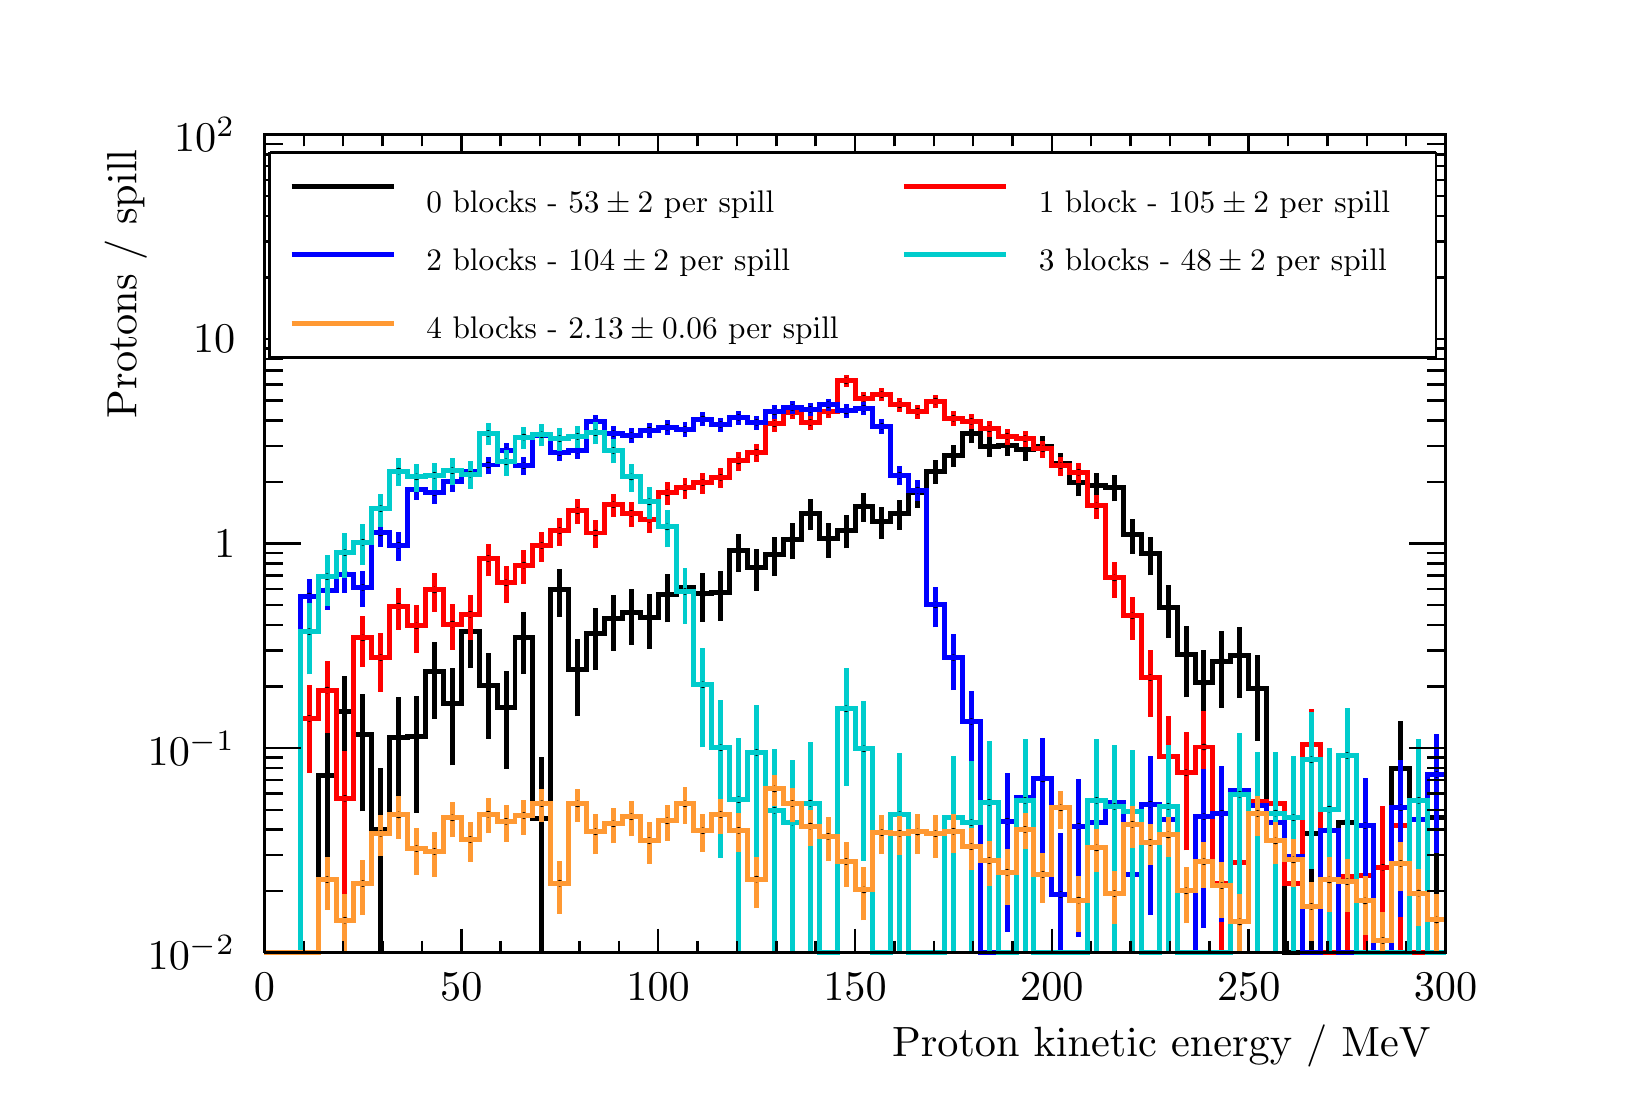
\begin{tikzpicture}
\pgfdeclareplotmark{cross} {
\pgfpathmoveto{\pgfpoint{-0.3\pgfplotmarksize}{\pgfplotmarksize}}
\pgfpathlineto{\pgfpoint{+0.3\pgfplotmarksize}{\pgfplotmarksize}}
\pgfpathlineto{\pgfpoint{+0.3\pgfplotmarksize}{0.3\pgfplotmarksize}}
\pgfpathlineto{\pgfpoint{+1\pgfplotmarksize}{0.3\pgfplotmarksize}}
\pgfpathlineto{\pgfpoint{+1\pgfplotmarksize}{-0.3\pgfplotmarksize}}
\pgfpathlineto{\pgfpoint{+0.3\pgfplotmarksize}{-0.3\pgfplotmarksize}}
\pgfpathlineto{\pgfpoint{+0.3\pgfplotmarksize}{-1.\pgfplotmarksize}}
\pgfpathlineto{\pgfpoint{-0.3\pgfplotmarksize}{-1.\pgfplotmarksize}}
\pgfpathlineto{\pgfpoint{-0.3\pgfplotmarksize}{-0.3\pgfplotmarksize}}
\pgfpathlineto{\pgfpoint{-1.\pgfplotmarksize}{-0.3\pgfplotmarksize}}
\pgfpathlineto{\pgfpoint{-1.\pgfplotmarksize}{0.3\pgfplotmarksize}}
\pgfpathlineto{\pgfpoint{-0.3\pgfplotmarksize}{0.3\pgfplotmarksize}}
\pgfpathclose
\pgfusepathqstroke
}
\pgfdeclareplotmark{cross*} {
\pgfpathmoveto{\pgfpoint{-0.3\pgfplotmarksize}{\pgfplotmarksize}}
\pgfpathlineto{\pgfpoint{+0.3\pgfplotmarksize}{\pgfplotmarksize}}
\pgfpathlineto{\pgfpoint{+0.3\pgfplotmarksize}{0.3\pgfplotmarksize}}
\pgfpathlineto{\pgfpoint{+1\pgfplotmarksize}{0.3\pgfplotmarksize}}
\pgfpathlineto{\pgfpoint{+1\pgfplotmarksize}{-0.3\pgfplotmarksize}}
\pgfpathlineto{\pgfpoint{+0.3\pgfplotmarksize}{-0.3\pgfplotmarksize}}
\pgfpathlineto{\pgfpoint{+0.3\pgfplotmarksize}{-1.\pgfplotmarksize}}
\pgfpathlineto{\pgfpoint{-0.3\pgfplotmarksize}{-1.\pgfplotmarksize}}
\pgfpathlineto{\pgfpoint{-0.3\pgfplotmarksize}{-0.3\pgfplotmarksize}}
\pgfpathlineto{\pgfpoint{-1.\pgfplotmarksize}{-0.3\pgfplotmarksize}}
\pgfpathlineto{\pgfpoint{-1.\pgfplotmarksize}{0.3\pgfplotmarksize}}
\pgfpathlineto{\pgfpoint{-0.3\pgfplotmarksize}{0.3\pgfplotmarksize}}
\pgfpathclose
\pgfusepathqfillstroke
}
\pgfdeclareplotmark{newstar} {
\pgfpathmoveto{\pgfqpoint{0pt}{\pgfplotmarksize}}
\pgfpathlineto{\pgfqpointpolar{44}{0.5\pgfplotmarksize}}
\pgfpathlineto{\pgfqpointpolar{18}{\pgfplotmarksize}}
\pgfpathlineto{\pgfqpointpolar{-20}{0.5\pgfplotmarksize}}
\pgfpathlineto{\pgfqpointpolar{-54}{\pgfplotmarksize}}
\pgfpathlineto{\pgfqpointpolar{-90}{0.5\pgfplotmarksize}}
\pgfpathlineto{\pgfqpointpolar{234}{\pgfplotmarksize}}
\pgfpathlineto{\pgfqpointpolar{198}{0.5\pgfplotmarksize}}
\pgfpathlineto{\pgfqpointpolar{162}{\pgfplotmarksize}}
\pgfpathlineto{\pgfqpointpolar{134}{0.5\pgfplotmarksize}}
\pgfpathclose
\pgfusepathqstroke
}
\pgfdeclareplotmark{newstar*} {
\pgfpathmoveto{\pgfqpoint{0pt}{\pgfplotmarksize}}
\pgfpathlineto{\pgfqpointpolar{44}{0.5\pgfplotmarksize}}
\pgfpathlineto{\pgfqpointpolar{18}{\pgfplotmarksize}}
\pgfpathlineto{\pgfqpointpolar{-20}{0.5\pgfplotmarksize}}
\pgfpathlineto{\pgfqpointpolar{-54}{\pgfplotmarksize}}
\pgfpathlineto{\pgfqpointpolar{-90}{0.5\pgfplotmarksize}}
\pgfpathlineto{\pgfqpointpolar{234}{\pgfplotmarksize}}
\pgfpathlineto{\pgfqpointpolar{198}{0.5\pgfplotmarksize}}
\pgfpathlineto{\pgfqpointpolar{162}{\pgfplotmarksize}}
\pgfpathlineto{\pgfqpointpolar{134}{0.5\pgfplotmarksize}}
\pgfpathclose
\pgfusepathqfillstroke
}
\definecolor{c}{rgb}{1,1,1};
\draw [color=c, fill=c] (0,0) rectangle (20,13.4957);
\draw [color=c, fill=c] (3,1.75444) rectangle (18,12.1461);
\definecolor{c}{rgb}{0,0,0};
\draw [c,line width=0.9] (3,1.75444) -- (3,12.1461) -- (18,12.1461) -- (18,1.75444) -- (3,1.75444);
\definecolor{c}{rgb}{1,1,1};
\draw [color=c, fill=c] (3,1.75444) rectangle (18,12.1461);
\definecolor{c}{rgb}{0,0,0};
\draw [c,line width=0.9] (3,1.75444) -- (3,12.1461) -- (18,12.1461) -- (18,1.75444) -- (3,1.75444);
\draw [c,line width=0.9] (3,1.75444) -- (3.22727,1.75444) -- (3.22727,1.75444) -- (3.45455,1.75444) -- (3.45455,1.75444) -- (3.68182,1.75444) -- (3.68182,1.75444) -- (3.90909,1.75444) -- (3.90909,1.75444) -- (4.13636,1.75444) -- (4.13636,1.75444) --
 (4.36364,1.75444) -- (4.36364,1.75444) -- (4.59091,1.75444) -- (4.59091,1.75444) -- (4.81818,1.75444) -- (4.81818,1.75444) -- (5.04545,1.75444) -- (5.04545,1.75444) -- (5.27273,1.75444) -- (5.27273,1.75444) -- (5.5,1.75444) -- (5.5,1.75444) --
 (5.72727,1.75444) -- (5.72727,1.75444) -- (5.95455,1.75444) -- (5.95455,1.75444) -- (6.18182,1.75444) -- (6.18182,1.75444) -- (6.40909,1.75444) -- (6.40909,1.75444) -- (6.63636,1.75444) -- (6.63636,1.75444) -- (6.86364,1.75444) -- (6.86364,1.75444)
 -- (7.09091,1.75444) -- (7.09091,1.75444) -- (7.31818,1.75444) -- (7.31818,1.75444) -- (7.54545,1.75444) -- (7.54545,1.75444) -- (7.77273,1.75444) -- (7.77273,1.75444) -- (8,1.75444) -- (8,1.75444) -- (8.22727,1.75444) -- (8.22727,1.75444) --
 (8.45455,1.75444) -- (8.45455,1.75444) -- (8.68182,1.75444) -- (8.68182,1.75444) -- (8.90909,1.75444) -- (8.90909,1.75444) -- (9.13636,1.75444) -- (9.13636,1.75444) -- (9.36364,1.75444) -- (9.36364,1.75444) -- (9.59091,1.75444) -- (9.59091,1.75444)
 -- (9.81818,1.75444) -- (9.81818,1.75444) -- (10.0455,1.75444) -- (10.0455,1.75444) -- (10.2727,1.75444) -- (10.2727,1.75444) -- (10.5,1.75444) -- (10.5,1.75444) -- (10.7273,1.75444) -- (10.7273,1.75444) -- (10.9545,1.75444) -- (10.9545,1.75444) --
 (11.1818,1.75444) -- (11.1818,1.75444) -- (11.4091,1.75444) -- (11.4091,1.75444) -- (11.6364,1.75444) -- (11.6364,1.75444) -- (11.8636,1.75444) -- (11.8636,1.75444) -- (12.0909,1.75444) -- (12.0909,1.75444) -- (12.3182,1.75444) -- (12.3182,1.75444)
 -- (12.5455,1.75444) -- (12.5455,1.75444) -- (12.7727,1.75444) -- (12.7727,1.75444) -- (13,1.75444) -- (13,1.75444) -- (13.2273,1.75444) -- (13.2273,1.75444) -- (13.4545,1.75444) -- (13.4545,1.75444) -- (13.6818,1.75444) -- (13.6818,1.75444) --
 (13.9091,1.75444) -- (13.9091,1.75444) -- (14.1364,1.75444) -- (14.1364,1.75444) -- (14.3636,1.75444) -- (14.3636,1.75444) -- (14.5909,1.75444) -- (14.5909,1.75444) -- (14.8182,1.75444) -- (14.8182,1.75444) -- (15.0455,1.75444) -- (15.0455,1.75444)
 -- (15.2727,1.75444) -- (15.2727,1.75444) -- (15.5,1.75444) -- (15.5,1.75444) -- (15.7273,1.75444) -- (15.7273,1.75444) -- (15.9545,1.75444) -- (15.9545,1.75444) -- (16.1818,1.75444) -- (16.1818,1.75444) -- (16.4091,1.75444) -- (16.4091,1.75444) --
 (16.6364,1.75444) -- (16.6364,1.75444) -- (16.8636,1.75444) -- (16.8636,1.75444) -- (17.0909,1.75444) -- (17.0909,1.75444) -- (17.3182,1.75444) -- (17.3182,1.75444) -- (17.5455,1.75444) -- (17.5455,1.75444) -- (17.7727,1.75444) -- (17.7727,1.75444)
 -- (18,1.75444);
\draw [c,line width=0.9] (3,1.75444) -- (18,1.75444);
\draw [c,line width=0.9] (3,2.05809) -- (3,1.75444);
\draw [c,line width=0.9] (3.5,1.90627) -- (3.5,1.75444);
\draw [c,line width=0.9] (4,1.90627) -- (4,1.75444);
\draw [c,line width=0.9] (4.5,1.90627) -- (4.5,1.75444);
\draw [c,line width=0.9] (5,1.90627) -- (5,1.75444);
\draw [c,line width=0.9] (5.5,2.05809) -- (5.5,1.75444);
\draw [c,line width=0.9] (6,1.90627) -- (6,1.75444);
\draw [c,line width=0.9] (6.5,1.90627) -- (6.5,1.75444);
\draw [c,line width=0.9] (7,1.90627) -- (7,1.75444);
\draw [c,line width=0.9] (7.5,1.90627) -- (7.5,1.75444);
\draw [c,line width=0.9] (8,2.05809) -- (8,1.75444);
\draw [c,line width=0.9] (8.5,1.90627) -- (8.5,1.75444);
\draw [c,line width=0.9] (9,1.90627) -- (9,1.75444);
\draw [c,line width=0.9] (9.5,1.90627) -- (9.5,1.75444);
\draw [c,line width=0.9] (10,1.90627) -- (10,1.75444);
\draw [c,line width=0.9] (10.5,2.05809) -- (10.5,1.75444);
\draw [c,line width=0.9] (11,1.90627) -- (11,1.75444);
\draw [c,line width=0.9] (11.5,1.90627) -- (11.5,1.75444);
\draw [c,line width=0.9] (12,1.90627) -- (12,1.75444);
\draw [c,line width=0.9] (12.5,1.90627) -- (12.5,1.75444);
\draw [c,line width=0.9] (13,2.05809) -- (13,1.75444);
\draw [c,line width=0.9] (13.5,1.90627) -- (13.5,1.75444);
\draw [c,line width=0.9] (14,1.90627) -- (14,1.75444);
\draw [c,line width=0.9] (14.5,1.90627) -- (14.5,1.75444);
\draw [c,line width=0.9] (15,1.90627) -- (15,1.75444);
\draw [c,line width=0.9] (15.5,2.05809) -- (15.5,1.75444);
\draw [c,line width=0.9] (16,1.90627) -- (16,1.75444);
\draw [c,line width=0.9] (16.5,1.90627) -- (16.5,1.75444);
\draw [c,line width=0.9] (17,1.90627) -- (17,1.75444);
\draw [c,line width=0.9] (17.5,1.90627) -- (17.5,1.75444);
\draw [c,line width=0.9] (18,2.05809) -- (18,1.75444);
\draw [c,line width=0.9] (18,2.05809) -- (18,1.75444);
\draw [anchor=base] (3,1.14713) node[scale=1.52731, color=c, rotate=0]{0};
\draw [anchor=base] (5.5,1.14713) node[scale=1.52731, color=c, rotate=0]{50};
\draw [anchor=base] (8,1.14713) node[scale=1.52731, color=c, rotate=0]{100};
\draw [anchor=base] (10.5,1.14713) node[scale=1.52731, color=c, rotate=0]{150};
\draw [anchor=base] (13,1.14713) node[scale=1.52731, color=c, rotate=0]{200};
\draw [anchor=base] (15.5,1.14713) node[scale=1.52731, color=c, rotate=0]{250};
\draw [anchor=base] (18,1.14713) node[scale=1.52731, color=c, rotate=0]{300};
\draw [anchor= east] (18,0.566819) node[scale=1.52731, color=c, rotate=0]{ Proton kinetic energy / MeV};
\draw [c,line width=0.9] (3,12.1461) -- (18,12.1461);
\draw [c,line width=0.9] (3,11.8425) -- (3,12.1461);
\draw [c,line width=0.9] (3.5,11.9943) -- (3.5,12.1461);
\draw [c,line width=0.9] (4,11.9943) -- (4,12.1461);
\draw [c,line width=0.9] (4.5,11.9943) -- (4.5,12.1461);
\draw [c,line width=0.9] (5,11.9943) -- (5,12.1461);
\draw [c,line width=0.9] (5.5,11.8425) -- (5.5,12.1461);
\draw [c,line width=0.9] (6,11.9943) -- (6,12.1461);
\draw [c,line width=0.9] (6.5,11.9943) -- (6.5,12.1461);
\draw [c,line width=0.9] (7,11.9943) -- (7,12.1461);
\draw [c,line width=0.9] (7.5,11.9943) -- (7.5,12.1461);
\draw [c,line width=0.9] (8,11.8425) -- (8,12.1461);
\draw [c,line width=0.9] (8.5,11.9943) -- (8.5,12.1461);
\draw [c,line width=0.9] (9,11.9943) -- (9,12.1461);
\draw [c,line width=0.9] (9.5,11.9943) -- (9.5,12.1461);
\draw [c,line width=0.9] (10,11.9943) -- (10,12.1461);
\draw [c,line width=0.9] (10.5,11.8425) -- (10.5,12.1461);
\draw [c,line width=0.9] (11,11.9943) -- (11,12.1461);
\draw [c,line width=0.9] (11.5,11.9943) -- (11.5,12.1461);
\draw [c,line width=0.9] (12,11.9943) -- (12,12.1461);
\draw [c,line width=0.9] (12.5,11.9943) -- (12.5,12.1461);
\draw [c,line width=0.9] (13,11.8425) -- (13,12.1461);
\draw [c,line width=0.9] (13.5,11.9943) -- (13.5,12.1461);
\draw [c,line width=0.9] (14,11.9943) -- (14,12.1461);
\draw [c,line width=0.9] (14.5,11.9943) -- (14.5,12.1461);
\draw [c,line width=0.9] (15,11.9943) -- (15,12.1461);
\draw [c,line width=0.9] (15.5,11.8425) -- (15.5,12.1461);
\draw [c,line width=0.9] (16,11.9943) -- (16,12.1461);
\draw [c,line width=0.9] (16.5,11.9943) -- (16.5,12.1461);
\draw [c,line width=0.9] (17,11.9943) -- (17,12.1461);
\draw [c,line width=0.9] (17.5,11.9943) -- (17.5,12.1461);
\draw [c,line width=0.9] (18,11.8425) -- (18,12.1461);
\draw [c,line width=0.9] (18,11.8425) -- (18,12.1461);
\draw [c,line width=0.9] (3,1.75444) -- (3,12.1461);
\draw [c,line width=0.9] (3.462,1.75444) -- (3,1.75444);
\draw [anchor= east] (2.82,1.75444) node[scale=1.52731, color=c, rotate=0]{$10^{-2}$};
\draw [c,line width=0.9] (3.231,2.5365) -- (3,2.5365);
\draw [c,line width=0.9] (3.231,2.99397) -- (3,2.99397);
\draw [c,line width=0.9] (3.231,3.31855) -- (3,3.31855);
\draw [c,line width=0.9] (3.231,3.57031) -- (3,3.57031);
\draw [c,line width=0.9] (3.231,3.77602) -- (3,3.77602);
\draw [c,line width=0.9] (3.231,3.94994) -- (3,3.94994);
\draw [c,line width=0.9] (3.231,4.1006) -- (3,4.1006);
\draw [c,line width=0.9] (3.231,4.23349) -- (3,4.23349);
\draw [c,line width=0.9] (3.462,4.35237) -- (3,4.35237);
\draw [anchor= east] (2.82,4.35237) node[scale=1.52731, color=c, rotate=0]{$10^{-1}$};
\draw [c,line width=0.9] (3.231,5.13442) -- (3,5.13442);
\draw [c,line width=0.9] (3.231,5.59189) -- (3,5.59189);
\draw [c,line width=0.9] (3.231,5.91647) -- (3,5.91647);
\draw [c,line width=0.9] (3.231,6.16824) -- (3,6.16824);
\draw [c,line width=0.9] (3.231,6.37394) -- (3,6.37394);
\draw [c,line width=0.9] (3.231,6.54786) -- (3,6.54786);
\draw [c,line width=0.9] (3.231,6.69852) -- (3,6.69852);
\draw [c,line width=0.9] (3.231,6.83141) -- (3,6.83141);
\draw [c,line width=0.9] (3.462,6.95029) -- (3,6.95029);
\draw [anchor= east] (2.82,6.95029) node[scale=1.52731, color=c, rotate=0]{1};
\draw [c,line width=0.9] (3.231,7.73234) -- (3,7.73234);
\draw [c,line width=0.9] (3.231,8.18981) -- (3,8.18981);
\draw [c,line width=0.9] (3.231,8.51439) -- (3,8.51439);
\draw [c,line width=0.9] (3.231,8.76616) -- (3,8.76616);
\draw [c,line width=0.9] (3.231,8.97186) -- (3,8.97186);
\draw [c,line width=0.9] (3.231,9.14579) -- (3,9.14579);
\draw [c,line width=0.9] (3.231,9.29644) -- (3,9.29644);
\draw [c,line width=0.9] (3.231,9.42934) -- (3,9.42934);
\draw [c,line width=0.9] (3.462,9.54821) -- (3,9.54821);
\draw [anchor= east] (2.82,9.54821) node[scale=1.52731, color=c, rotate=0]{10};
\draw [c,line width=0.9] (3.231,10.3303) -- (3,10.3303);
\draw [c,line width=0.9] (3.231,10.7877) -- (3,10.7877);
\draw [c,line width=0.9] (3.231,11.1123) -- (3,11.1123);
\draw [c,line width=0.9] (3.231,11.3641) -- (3,11.3641);
\draw [c,line width=0.9] (3.231,11.5698) -- (3,11.5698);
\draw [c,line width=0.9] (3.231,11.7437) -- (3,11.7437);
\draw [c,line width=0.9] (3.231,11.8944) -- (3,11.8944);
\draw [c,line width=0.9] (3.231,12.0273) -- (3,12.0273);
\draw [c,line width=0.9] (3.462,12.1461) -- (3,12.1461);
\draw [anchor= east] (2.82,12.1461) node[scale=1.52731, color=c, rotate=0]{$10^{2}$};
\draw [anchor= east] (1.24,12.1461) node[scale=1.52731, color=c, rotate=90]{ Protons / spill};
\draw [c,line width=0.9] (18,1.75444) -- (18,12.1461);
\draw [c,line width=0.9] (17.538,1.75444) -- (18,1.75444);
\draw [c,line width=0.9] (17.769,2.5365) -- (18,2.5365);
\draw [c,line width=0.9] (17.769,2.99397) -- (18,2.99397);
\draw [c,line width=0.9] (17.769,3.31855) -- (18,3.31855);
\draw [c,line width=0.9] (17.769,3.57031) -- (18,3.57031);
\draw [c,line width=0.9] (17.769,3.77602) -- (18,3.77602);
\draw [c,line width=0.9] (17.769,3.94994) -- (18,3.94994);
\draw [c,line width=0.9] (17.769,4.1006) -- (18,4.1006);
\draw [c,line width=0.9] (17.769,4.23349) -- (18,4.23349);
\draw [c,line width=0.9] (17.538,4.35237) -- (18,4.35237);
\draw [c,line width=0.9] (17.769,5.13442) -- (18,5.13442);
\draw [c,line width=0.9] (17.769,5.59189) -- (18,5.59189);
\draw [c,line width=0.9] (17.769,5.91647) -- (18,5.91647);
\draw [c,line width=0.9] (17.769,6.16824) -- (18,6.16824);
\draw [c,line width=0.9] (17.769,6.37394) -- (18,6.37394);
\draw [c,line width=0.9] (17.769,6.54786) -- (18,6.54786);
\draw [c,line width=0.9] (17.769,6.69852) -- (18,6.69852);
\draw [c,line width=0.9] (17.769,6.83141) -- (18,6.83141);
\draw [c,line width=0.9] (17.538,6.95029) -- (18,6.95029);
\draw [c,line width=0.9] (17.769,7.73234) -- (18,7.73234);
\draw [c,line width=0.9] (17.769,8.18981) -- (18,8.18981);
\draw [c,line width=0.9] (17.769,8.51439) -- (18,8.51439);
\draw [c,line width=0.9] (17.769,8.76616) -- (18,8.76616);
\draw [c,line width=0.9] (17.769,8.97186) -- (18,8.97186);
\draw [c,line width=0.9] (17.769,9.14579) -- (18,9.14579);
\draw [c,line width=0.9] (17.769,9.29644) -- (18,9.29644);
\draw [c,line width=0.9] (17.769,9.42934) -- (18,9.42934);
\draw [c,line width=0.9] (17.538,9.54821) -- (18,9.54821);
\draw [c,line width=0.9] (17.769,10.3303) -- (18,10.3303);
\draw [c,line width=0.9] (17.769,10.7877) -- (18,10.7877);
\draw [c,line width=0.9] (17.769,11.1123) -- (18,11.1123);
\draw [c,line width=0.9] (17.769,11.3641) -- (18,11.3641);
\draw [c,line width=0.9] (17.769,11.5698) -- (18,11.5698);
\draw [c,line width=0.9] (17.769,11.7437) -- (18,11.7437);
\draw [c,line width=0.9] (17.769,11.8944) -- (18,11.8944);
\draw [c,line width=0.9] (17.769,12.0273) -- (18,12.0273);
\draw [c,line width=0.9] (17.538,12.1461) -- (18,12.1461);
\draw [c,line width=1.8] (3.79545,2.60924) -- (3.79545,4.00539);
\draw [c,line width=1.8] (3.79545,4.00539) -- (3.79545,4.61061);
\foreach \P in {(3.79545,4.00539)}{\draw[mark options={color=c,fill=c},mark size=2.402402pt,mark=*,mark size=1pt] plot coordinates {\P};}
\draw [c,line width=1.8] (4.02273,4.03114) -- (4.02273,4.81428);
\draw [c,line width=1.8] (4.02273,4.81428) -- (4.02273,5.27211);
\foreach \P in {(4.02273,4.81428)}{\draw[mark options={color=c,fill=c},mark size=2.402402pt,mark=*,mark size=1pt] plot coordinates {\P};}
\draw [c,line width=1.8] (4.25,3.5497) -- (4.25,4.52289);
\draw [c,line width=1.8] (4.25,4.52289) -- (4.25,5.0375);
\foreach \P in {(4.25,4.52289)}{\draw[mark options={color=c,fill=c},mark size=2.402402pt,mark=*,mark size=1pt] plot coordinates {\P};}
\draw [c,line width=1.8] (4.47727,1.75444) -- (4.47727,3.32318);
\draw [c,line width=1.8] (4.47727,3.32318) -- (4.47727,4.10524);
\foreach \P in {(4.47727,3.32318)}{\draw[mark options={color=c,fill=c},mark size=2.402402pt,mark=*,mark size=1pt] plot coordinates {\P};}
\draw [c,line width=1.8] (4.70455,3.51188) -- (4.70455,4.48763);
\draw [c,line width=1.8] (4.70455,4.48763) -- (4.70455,5.00292);
\foreach \P in {(4.70455,4.48763)}{\draw[mark options={color=c,fill=c},mark size=2.402402pt,mark=*,mark size=1pt] plot coordinates {\P};}
\draw [c,line width=1.8] (4.93182,3.5301) -- (4.93182,4.50411);
\draw [c,line width=1.8] (4.93182,4.50411) -- (4.93182,5.01894);
\foreach \P in {(4.93182,4.50411)}{\draw[mark options={color=c,fill=c},mark size=2.402402pt,mark=*,mark size=1pt] plot coordinates {\P};}
\draw [c,line width=1.8] (5.15909,4.72595) -- (5.15909,5.31984);
\draw [c,line width=1.8] (5.15909,5.31984) -- (5.15909,5.7069);
\foreach \P in {(5.15909,5.31984)}{\draw[mark options={color=c,fill=c},mark size=2.402402pt,mark=*,mark size=1pt] plot coordinates {\P};}
\draw [c,line width=1.8] (5.38636,4.13231) -- (5.38636,4.91521);
\draw [c,line width=1.8] (5.38636,4.91521) -- (5.38636,5.37296);
\foreach \P in {(5.38636,4.91521)}{\draw[mark options={color=c,fill=c},mark size=2.402402pt,mark=*,mark size=1pt] plot coordinates {\P};}
\draw [c,line width=1.8] (5.61364,5.36765) -- (5.61364,5.8311);
\draw [c,line width=1.8] (5.61364,5.8311) -- (5.61364,6.15865);
\foreach \P in {(5.61364,5.8311)}{\draw[mark options={color=c,fill=c},mark size=2.402402pt,mark=*,mark size=1pt] plot coordinates {\P};}
\draw [c,line width=1.8] (5.84091,4.47369) -- (5.84091,5.14585);
\draw [c,line width=1.8] (5.84091,5.14585) -- (5.84091,5.56418);
\foreach \P in {(5.84091,5.14585)}{\draw[mark options={color=c,fill=c},mark size=2.402402pt,mark=*,mark size=1pt] plot coordinates {\P};}
\draw [c,line width=1.8] (6.06818,4.08623) -- (6.06818,4.8698);
\draw [c,line width=1.8] (6.06818,4.8698) -- (6.06818,5.32777);
\foreach \P in {(6.06818,4.8698)}{\draw[mark options={color=c,fill=c},mark size=2.402402pt,mark=*,mark size=1pt] plot coordinates {\P};}
\draw [c,line width=1.8] (6.29545,5.29359) -- (6.29545,5.75425);
\draw [c,line width=1.8] (6.29545,5.75425) -- (6.29545,6.08042);
\foreach \P in {(6.29545,5.75425)}{\draw[mark options={color=c,fill=c},mark size=2.402402pt,mark=*,mark size=1pt] plot coordinates {\P};}
\draw [c,line width=1.8] (6.52273,1.75444) -- (6.52273,3.46448);
\draw [c,line width=1.8] (6.52273,3.46448) -- (6.52273,4.24653);
\foreach \P in {(6.52273,3.46448)}{\draw[mark options={color=c,fill=c},mark size=2.402402pt,mark=*,mark size=1pt] plot coordinates {\P};}
\draw [c,line width=1.8] (6.75,6.02252) -- (6.75,6.36177);
\draw [c,line width=1.8] (6.75,6.36177) -- (6.75,6.62224);
\foreach \P in {(6.75,6.36177)}{\draw[mark options={color=c,fill=c},mark size=2.402402pt,mark=*,mark size=1pt] plot coordinates {\P};}
\draw [c,line width=1.8] (6.97727,4.75616) -- (6.97727,5.34913);
\draw [c,line width=1.8] (6.97727,5.34913) -- (6.97727,5.73582);
\foreach \P in {(6.97727,5.34913)}{\draw[mark options={color=c,fill=c},mark size=2.402402pt,mark=*,mark size=1pt] plot coordinates {\P};}
\draw [c,line width=1.8] (7.20455,5.34851) -- (7.20455,5.80911);
\draw [c,line width=1.8] (7.20455,5.80911) -- (7.20455,6.13526);
\foreach \P in {(7.20455,5.80911)}{\draw[mark options={color=c,fill=c},mark size=2.402402pt,mark=*,mark size=1pt] plot coordinates {\P};}
\draw [c,line width=1.8] (7.43182,5.58905) -- (7.43182,5.99782);
\draw [c,line width=1.8] (7.43182,5.99782) -- (7.43182,6.29724);
\foreach \P in {(7.43182,5.99782)}{\draw[mark options={color=c,fill=c},mark size=2.402402pt,mark=*,mark size=1pt] plot coordinates {\P};}
\draw [c,line width=1.8] (7.65909,5.66385) -- (7.65909,6.07109);
\draw [c,line width=1.8] (7.65909,6.07109) -- (7.65909,6.36969);
\foreach \P in {(7.65909,6.07109)}{\draw[mark options={color=c,fill=c},mark size=2.402402pt,mark=*,mark size=1pt] plot coordinates {\P};}
\draw [c,line width=1.8] (7.88636,5.61049) -- (7.88636,6.01595);
\draw [c,line width=1.8] (7.88636,6.01595) -- (7.88636,6.3136);
\foreach \P in {(7.88636,6.01595)}{\draw[mark options={color=c,fill=c},mark size=2.402402pt,mark=*,mark size=1pt] plot coordinates {\P};}
\draw [c,line width=1.8] (8.11364,5.94903) -- (8.11364,6.30148);
\draw [c,line width=1.8] (8.11364,6.30148) -- (8.11364,6.56965);
\foreach \P in {(8.11364,6.30148)}{\draw[mark options={color=c,fill=c},mark size=2.402402pt,mark=*,mark size=1pt] plot coordinates {\P};}
\draw [c,line width=1.8] (8.34091,6.06278) -- (8.34091,6.38842);
\draw [c,line width=1.8] (8.34091,6.38842) -- (8.34091,6.64082);
\foreach \P in {(8.34091,6.38842)}{\draw[mark options={color=c,fill=c},mark size=2.402402pt,mark=*,mark size=1pt] plot coordinates {\P};}
\draw [c,line width=1.8] (8.56818,5.95652) -- (8.56818,6.31043);
\draw [c,line width=1.8] (8.56818,6.31043) -- (8.56818,6.57943);
\foreach \P in {(8.56818,6.31043)}{\draw[mark options={color=c,fill=c},mark size=2.402402pt,mark=*,mark size=1pt] plot coordinates {\P};}
\draw [c,line width=1.8] (8.79545,5.97304) -- (8.79545,6.32748);
\draw [c,line width=1.8] (8.79545,6.32748) -- (8.79545,6.5968);
\foreach \P in {(8.79545,6.32748)}{\draw[mark options={color=c,fill=c},mark size=2.402402pt,mark=*,mark size=1pt] plot coordinates {\P};}
\draw [c,line width=1.8] (9.02273,6.5917) -- (9.02273,6.85685);
\draw [c,line width=1.8] (9.02273,6.85685) -- (9.02273,7.07139);
\foreach \P in {(9.02273,6.85685)}{\draw[mark options={color=c,fill=c},mark size=2.402402pt,mark=*,mark size=1pt] plot coordinates {\P};}
\draw [c,line width=1.8] (9.25,6.34879) -- (9.25,6.64525);
\draw [c,line width=1.8] (9.25,6.64525) -- (9.25,6.8798);
\foreach \P in {(9.25,6.64525)}{\draw[mark options={color=c,fill=c},mark size=2.402402pt,mark=*,mark size=1pt] plot coordinates {\P};}
\draw [c,line width=1.8] (9.47727,6.5369) -- (9.47727,6.81036);
\draw [c,line width=1.8] (9.47727,6.81036) -- (9.47727,7.0303);
\foreach \P in {(9.47727,6.81036)}{\draw[mark options={color=c,fill=c},mark size=2.402402pt,mark=*,mark size=1pt] plot coordinates {\P};}
\draw [c,line width=1.8] (9.70455,6.7599) -- (9.70455,7.00766);
\draw [c,line width=1.8] (9.70455,7.00766) -- (9.70455,7.21069);
\foreach \P in {(9.70455,7.00766)}{\draw[mark options={color=c,fill=c},mark size=2.402402pt,mark=*,mark size=1pt] plot coordinates {\P};}
\draw [c,line width=1.8] (9.93182,7.12677) -- (9.93182,7.33707);
\draw [c,line width=1.8] (9.93182,7.33707) -- (9.93182,7.51427);
\foreach \P in {(9.93182,7.33707)}{\draw[mark options={color=c,fill=c},mark size=2.402402pt,mark=*,mark size=1pt] plot coordinates {\P};}
\draw [c,line width=1.8] (10.1591,6.7687) -- (10.1591,7.01088);
\draw [c,line width=1.8] (10.1591,7.01088) -- (10.1591,7.21015);
\foreach \P in {(10.1591,7.01088)}{\draw[mark options={color=c,fill=c},mark size=2.402402pt,mark=*,mark size=1pt] plot coordinates {\P};}
\draw [c,line width=1.8] (10.3864,6.88913) -- (10.3864,7.11788);
\draw [c,line width=1.8] (10.3864,7.11788) -- (10.3864,7.30797);
\foreach \P in {(10.3864,7.11788)}{\draw[mark options={color=c,fill=c},mark size=2.402402pt,mark=*,mark size=1pt] plot coordinates {\P};}
\draw [c,line width=1.8] (10.6136,7.22852) -- (10.6136,7.42613);
\draw [c,line width=1.8] (10.6136,7.42613) -- (10.6136,7.59423);
\foreach \P in {(10.6136,7.42613)}{\draw[mark options={color=c,fill=c},mark size=2.402402pt,mark=*,mark size=1pt] plot coordinates {\P};}
\draw [c,line width=1.8] (10.8409,7.0079) -- (10.8409,7.22835);
\draw [c,line width=1.8] (10.8409,7.22835) -- (10.8409,7.41268);
\foreach \P in {(10.8409,7.22835)}{\draw[mark options={color=c,fill=c},mark size=2.402402pt,mark=*,mark size=1pt] plot coordinates {\P};}
\draw [c,line width=1.8] (11.0682,7.12833) -- (11.0682,7.33525);
\draw [c,line width=1.8] (11.0682,7.33525) -- (11.0682,7.51005);
\foreach \P in {(11.0682,7.33525)}{\draw[mark options={color=c,fill=c},mark size=2.402402pt,mark=*,mark size=1pt] plot coordinates {\P};}
\draw [c,line width=1.8] (11.2955,7.40746) -- (11.2955,7.59292);
\draw [c,line width=1.8] (11.2955,7.59292) -- (11.2955,7.75215);
\foreach \P in {(11.2955,7.59292)}{\draw[mark options={color=c,fill=c},mark size=2.402402pt,mark=*,mark size=1pt] plot coordinates {\P};}
\draw [c,line width=1.8] (11.5227,7.70421) -- (11.5227,7.86713);
\draw [c,line width=1.8] (11.5227,7.86713) -- (11.5227,8.00947);
\foreach \P in {(11.5227,7.86713)}{\draw[mark options={color=c,fill=c},mark size=2.402402pt,mark=*,mark size=1pt] plot coordinates {\P};}
\draw [c,line width=1.8] (11.75,7.92009) -- (11.75,8.06794);
\draw [c,line width=1.8] (11.75,8.06794) -- (11.75,8.19864);
\foreach \P in {(11.75,8.06794)}{\draw[mark options={color=c,fill=c},mark size=2.402402pt,mark=*,mark size=1pt] plot coordinates {\P};}
\draw [c,line width=1.8] (11.9773,8.22288) -- (11.9773,8.3524);
\draw [c,line width=1.8] (11.9773,8.3524) -- (11.9773,8.46858);
\foreach \P in {(11.9773,8.3524)}{\draw[mark options={color=c,fill=c},mark size=2.402402pt,mark=*,mark size=1pt] plot coordinates {\P};}
\draw [c,line width=1.8] (12.2045,8.04755) -- (12.2045,8.18769);
\draw [c,line width=1.8] (12.2045,8.18769) -- (12.2045,8.31234);
\foreach \P in {(12.2045,8.18769)}{\draw[mark options={color=c,fill=c},mark size=2.402402pt,mark=*,mark size=1pt] plot coordinates {\P};}
\draw [c,line width=1.8] (12.4318,8.06348) -- (12.4318,8.20158);
\draw [c,line width=1.8] (12.4318,8.20158) -- (12.4318,8.32461);
\foreach \P in {(12.4318,8.20158)}{\draw[mark options={color=c,fill=c},mark size=2.402402pt,mark=*,mark size=1pt] plot coordinates {\P};}
\draw [c,line width=1.8] (12.6591,7.9996) -- (12.6591,8.14294);
\draw [c,line width=1.8] (12.6591,8.14294) -- (12.6591,8.27011);
\foreach \P in {(12.6591,8.14294)}{\draw[mark options={color=c,fill=c},mark size=2.402402pt,mark=*,mark size=1pt] plot coordinates {\P};}
\draw [c,line width=1.8] (12.8864,8.04758) -- (12.8864,8.18805);
\draw [c,line width=1.8] (12.8864,8.18805) -- (12.8864,8.31296);
\foreach \P in {(12.8864,8.18805)}{\draw[mark options={color=c,fill=c},mark size=2.402402pt,mark=*,mark size=1pt] plot coordinates {\P};}
\draw [c,line width=1.8] (13.1136,7.81831) -- (13.1136,7.97079);
\draw [c,line width=1.8] (13.1136,7.97079) -- (13.1136,8.10509);
\foreach \P in {(13.1136,7.97079)}{\draw[mark options={color=c,fill=c},mark size=2.402402pt,mark=*,mark size=1pt] plot coordinates {\P};}
\draw [c,line width=1.8] (13.3409,7.55089) -- (13.3409,7.72195);
\draw [c,line width=1.8] (13.3409,7.72195) -- (13.3409,7.87046);
\foreach \P in {(13.3409,7.72195)}{\draw[mark options={color=c,fill=c},mark size=2.402402pt,mark=*,mark size=1pt] plot coordinates {\P};}
\draw [c,line width=1.8] (13.5682,7.5121) -- (13.5682,7.68905);
\draw [c,line width=1.8] (13.5682,7.68905) -- (13.5682,7.84197);
\foreach \P in {(13.5682,7.68905)}{\draw[mark options={color=c,fill=c},mark size=2.402402pt,mark=*,mark size=1pt] plot coordinates {\P};}
\draw [c,line width=1.8] (13.7955,7.48592) -- (13.7955,7.66469);
\draw [c,line width=1.8] (13.7955,7.66469) -- (13.7955,7.81896);
\foreach \P in {(13.7955,7.66469)}{\draw[mark options={color=c,fill=c},mark size=2.402402pt,mark=*,mark size=1pt] plot coordinates {\P};}
\draw [c,line width=1.8] (14.0227,6.81875) -- (14.0227,7.06169);
\draw [c,line width=1.8] (14.0227,7.06169) -- (14.0227,7.26147);
\foreach \P in {(14.0227,7.06169)}{\draw[mark options={color=c,fill=c},mark size=2.402402pt,mark=*,mark size=1pt] plot coordinates {\P};}
\draw [c,line width=1.8] (14.25,6.54671) -- (14.25,6.81855);
\draw [c,line width=1.8] (14.25,6.81855) -- (14.25,7.03744);
\foreach \P in {(14.25,6.81855)}{\draw[mark options={color=c,fill=c},mark size=2.402402pt,mark=*,mark size=1pt] plot coordinates {\P};}
\draw [c,line width=1.8] (14.4773,5.75068) -- (14.4773,6.13666);
\draw [c,line width=1.8] (14.4773,6.13666) -- (14.4773,6.42371);
\foreach \P in {(14.4773,6.13666)}{\draw[mark options={color=c,fill=c},mark size=2.402402pt,mark=*,mark size=1pt] plot coordinates {\P};}
\draw [c,line width=1.8] (14.7045,4.99765) -- (14.7045,5.53879);
\draw [c,line width=1.8] (14.7045,5.53879) -- (14.7045,5.90299);
\foreach \P in {(14.7045,5.53879)}{\draw[mark options={color=c,fill=c},mark size=2.402402pt,mark=*,mark size=1pt] plot coordinates {\P};}
\draw [c,line width=1.8] (14.9318,4.50266) -- (14.9318,5.18182);
\draw [c,line width=1.8] (14.9318,5.18182) -- (14.9318,5.6028);
\foreach \P in {(14.9318,5.18182)}{\draw[mark options={color=c,fill=c},mark size=2.402402pt,mark=*,mark size=1pt] plot coordinates {\P};}
\draw [c,line width=1.8] (15.1591,4.86338) -- (15.1591,5.45838);
\draw [c,line width=1.8] (15.1591,5.45838) -- (15.1591,5.84591);
\foreach \P in {(15.1591,5.45838)}{\draw[mark options={color=c,fill=c},mark size=2.402402pt,mark=*,mark size=1pt] plot coordinates {\P};}
\draw [c,line width=1.8] (15.3864,4.99129) -- (15.3864,5.5324);
\draw [c,line width=1.8] (15.3864,5.5324) -- (15.3864,5.89658);
\foreach \P in {(15.3864,5.5324)}{\draw[mark options={color=c,fill=c},mark size=2.402402pt,mark=*,mark size=1pt] plot coordinates {\P};}
\draw [c,line width=1.8] (15.6136,4.44511) -- (15.6136,5.11566);
\draw [c,line width=1.8] (15.6136,5.11566) -- (15.6136,5.53337);
\foreach \P in {(15.6136,5.11566)}{\draw[mark options={color=c,fill=c},mark size=2.402402pt,mark=*,mark size=1pt] plot coordinates {\P};}
\draw [c,line width=1.8] (15.8409,1.75444) -- (15.8409,3.17557);
\draw [c,line width=1.8] (15.8409,3.17557) -- (15.8409,3.95762);
\foreach \P in {(15.8409,3.17557)}{\draw[mark options={color=c,fill=c},mark size=2.402402pt,mark=*,mark size=1pt] plot coordinates {\P};}
\draw [c,line width=1.8] (16.2955,1.75444) -- (16.2955,3.26653);
\draw [c,line width=1.8] (16.2955,3.26653) -- (16.2955,4.04858);
\foreach \P in {(16.2955,3.26653)}{\draw[mark options={color=c,fill=c},mark size=2.402402pt,mark=*,mark size=1pt] plot coordinates {\P};}
\draw [c,line width=1.8] (16.75,1.75444) -- (16.75,3.41388);
\draw [c,line width=1.8] (16.75,3.41388) -- (16.75,4.19594);
\foreach \P in {(16.75,3.41388)}{\draw[mark options={color=c,fill=c},mark size=2.402402pt,mark=*,mark size=1pt] plot coordinates {\P};}
\draw [c,line width=1.8] (17.4318,2.69824) -- (17.4318,4.08945);
\draw [c,line width=1.8] (17.4318,4.08945) -- (17.4318,4.69383);
\foreach \P in {(17.4318,4.08945)}{\draw[mark options={color=c,fill=c},mark size=2.402402pt,mark=*,mark size=1pt] plot coordinates {\P};}
\draw [c,line width=1.8] (17.8864,1.75444) -- (17.8864,3.46919);
\draw [c,line width=1.8] (17.8864,3.46919) -- (17.8864,4.25124);
\foreach \P in {(17.8864,3.46919)}{\draw[mark options={color=c,fill=c},mark size=2.402402pt,mark=*,mark size=1pt] plot coordinates {\P};}
\draw [c,line width=1.8] (3,1.75444) -- (3.22727,1.75444) -- (3.22727,1.75444) -- (3.45455,1.75444) -- (3.45455,1.75444) -- (3.68182,1.75444) -- (3.68182,4.00539) -- (3.90909,4.00539) -- (3.90909,4.81428) -- (4.13636,4.81428) -- (4.13636,4.52289) --
 (4.36364,4.52289) -- (4.36364,3.32318) -- (4.59091,3.32318) -- (4.59091,4.48763) -- (4.81818,4.48763) -- (4.81818,4.50411) -- (5.04545,4.50411) -- (5.04545,5.31984) -- (5.27273,5.31984) -- (5.27273,4.91521) -- (5.5,4.91521) -- (5.5,5.8311) --
 (5.72727,5.8311) -- (5.72727,5.14585) -- (5.95455,5.14585) -- (5.95455,4.8698) -- (6.18182,4.8698) -- (6.18182,5.75425) -- (6.40909,5.75425) -- (6.40909,3.46448) -- (6.63636,3.46448) -- (6.63636,6.36177) -- (6.86364,6.36177) -- (6.86364,5.34913) --
 (7.09091,5.34913) -- (7.09091,5.80911) -- (7.31818,5.80911) -- (7.31818,5.99782) -- (7.54545,5.99782) -- (7.54545,6.07109) -- (7.77273,6.07109) -- (7.77273,6.01595) -- (8,6.01595) -- (8,6.30148) -- (8.22727,6.30148) -- (8.22727,6.38842) --
 (8.45455,6.38842) -- (8.45455,6.31043) -- (8.68182,6.31043) -- (8.68182,6.32748) -- (8.90909,6.32748) -- (8.90909,6.85685) -- (9.13636,6.85685) -- (9.13636,6.64525) -- (9.36364,6.64525) -- (9.36364,6.81036) -- (9.59091,6.81036) -- (9.59091,7.00766)
 -- (9.81818,7.00766) -- (9.81818,7.33707) -- (10.0455,7.33707) -- (10.0455,7.01088) -- (10.2727,7.01088) -- (10.2727,7.11788) -- (10.5,7.11788) -- (10.5,7.42613) -- (10.7273,7.42613) -- (10.7273,7.22835) -- (10.9545,7.22835) -- (10.9545,7.33525) --
 (11.1818,7.33525) -- (11.1818,7.59292) -- (11.4091,7.59292) -- (11.4091,7.86713) -- (11.6364,7.86713) -- (11.6364,8.06794) -- (11.8636,8.06794) -- (11.8636,8.3524) -- (12.0909,8.3524) -- (12.0909,8.18769) -- (12.3182,8.18769) -- (12.3182,8.20158) --
 (12.5455,8.20158) -- (12.5455,8.14294) -- (12.7727,8.14294) -- (12.7727,8.18805) -- (13,8.18805) -- (13,7.97079) -- (13.2273,7.97079) -- (13.2273,7.72195) -- (13.4545,7.72195) -- (13.4545,7.68905) -- (13.6818,7.68905) -- (13.6818,7.66469) --
 (13.9091,7.66469) -- (13.9091,7.06169) -- (14.1364,7.06169) -- (14.1364,6.81855) -- (14.3636,6.81855) -- (14.3636,6.13666) -- (14.5909,6.13666) -- (14.5909,5.53879) -- (14.8182,5.53879) -- (14.8182,5.18182) -- (15.0455,5.18182) -- (15.0455,5.45838)
 -- (15.2727,5.45838) -- (15.2727,5.5324) -- (15.5,5.5324) -- (15.5,5.11566) -- (15.7273,5.11566) -- (15.7273,3.17557) -- (15.9545,3.17557) -- (15.9545,1.75444) -- (16.1818,1.75444) -- (16.1818,3.26653) -- (16.4091,3.26653) -- (16.4091,1.75444) --
 (16.6364,1.75444) -- (16.6364,3.41388) -- (16.8636,3.41388) -- (16.8636,1.75444) -- (17.0909,1.75444) -- (17.0909,1.75444) -- (17.3182,1.75444) -- (17.3182,4.08945) -- (17.5455,4.08945) -- (17.5455,1.75444) -- (17.7727,1.75444) -- (17.7727,3.46919)
 -- (18,3.46919);
\definecolor{c}{rgb}{1,0,0};
\draw [c,line width=1.8] (3.56818,4.04233) -- (3.56818,4.73002);
\draw [c,line width=1.8] (3.56818,4.73002) -- (3.56818,5.15419);
\definecolor{c}{rgb}{0,0,0};
\foreach \P in {(3.56818,4.73002)}{\draw[mark options={color=c,fill=c},mark size=2.402402pt,mark=*,mark size=1pt] plot coordinates {\P};}
\definecolor{c}{rgb}{1,0,0};
\draw [c,line width=1.8] (3.79545,4.5476) -- (3.79545,5.09077);
\draw [c,line width=1.8] (3.79545,5.09077) -- (3.79545,5.45588);
\definecolor{c}{rgb}{0,0,0};
\foreach \P in {(3.79545,5.09077)}{\draw[mark options={color=c,fill=c},mark size=2.402402pt,mark=*,mark size=1pt] plot coordinates {\P};}
\definecolor{c}{rgb}{1,0,0};
\draw [c,line width=1.8] (4.02273,2.32359) -- (4.02273,3.71481);
\draw [c,line width=1.8] (4.02273,3.71481) -- (4.02273,4.31919);
\definecolor{c}{rgb}{0,0,0};
\foreach \P in {(4.02273,3.71481)}{\draw[mark options={color=c,fill=c},mark size=2.402402pt,mark=*,mark size=1pt] plot coordinates {\P};}
\definecolor{c}{rgb}{1,0,0};
\draw [c,line width=1.8] (4.25,5.38034) -- (4.25,5.75291);
\draw [c,line width=1.8] (4.25,5.75291) -- (4.25,6.03253);
\definecolor{c}{rgb}{0,0,0};
\foreach \P in {(4.25,5.75291)}{\draw[mark options={color=c,fill=c},mark size=2.402402pt,mark=*,mark size=1pt] plot coordinates {\P};}
\definecolor{c}{rgb}{1,0,0};
\draw [c,line width=1.8] (4.47727,5.06878) -- (4.47727,5.50201);
\draw [c,line width=1.8] (4.47727,5.50201) -- (4.47727,5.81427);
\definecolor{c}{rgb}{0,0,0};
\foreach \P in {(4.47727,5.50201)}{\draw[mark options={color=c,fill=c},mark size=2.402402pt,mark=*,mark size=1pt] plot coordinates {\P};}
\definecolor{c}{rgb}{1,0,0};
\draw [c,line width=1.8] (4.70455,5.85764) -- (4.70455,6.15627);
\draw [c,line width=1.8] (4.70455,6.15627) -- (4.70455,6.39218);
\definecolor{c}{rgb}{0,0,0};
\foreach \P in {(4.70455,6.15627)}{\draw[mark options={color=c,fill=c},mark size=2.402402pt,mark=*,mark size=1pt] plot coordinates {\P};}
\definecolor{c}{rgb}{1,0,0};
\draw [c,line width=1.8] (4.93182,5.56026) -- (4.93182,5.90519);
\draw [c,line width=1.8] (4.93182,5.90519) -- (4.93182,6.16899);
\definecolor{c}{rgb}{0,0,0};
\foreach \P in {(4.93182,5.90519)}{\draw[mark options={color=c,fill=c},mark size=2.402402pt,mark=*,mark size=1pt] plot coordinates {\P};}
\definecolor{c}{rgb}{1,0,0};
\draw [c,line width=1.8] (5.15909,6.08567) -- (5.15909,6.36135);
\draw [c,line width=1.8] (5.15909,6.36135) -- (5.15909,6.58273);
\definecolor{c}{rgb}{0,0,0};
\foreach \P in {(5.15909,6.36135)}{\draw[mark options={color=c,fill=c},mark size=2.402402pt,mark=*,mark size=1pt] plot coordinates {\P};}
\definecolor{c}{rgb}{1,0,0};
\draw [c,line width=1.8] (5.38636,5.60087) -- (5.38636,5.92915);
\draw [c,line width=1.8] (5.38636,5.92915) -- (5.38636,6.18314);
\definecolor{c}{rgb}{0,0,0};
\foreach \P in {(5.38636,5.92915)}{\draw[mark options={color=c,fill=c},mark size=2.402402pt,mark=*,mark size=1pt] plot coordinates {\P};}
\definecolor{c}{rgb}{1,0,0};
\draw [c,line width=1.8] (5.61364,5.73173) -- (5.61364,6.05263);
\draw [c,line width=1.8] (5.61364,6.05263) -- (5.61364,6.30218);
\definecolor{c}{rgb}{0,0,0};
\foreach \P in {(5.61364,6.05263)}{\draw[mark options={color=c,fill=c},mark size=2.402402pt,mark=*,mark size=1pt] plot coordinates {\P};}
\definecolor{c}{rgb}{1,0,0};
\draw [c,line width=1.8] (5.84091,6.53542) -- (5.84091,6.76106);
\draw [c,line width=1.8] (5.84091,6.76106) -- (5.84091,6.94901);
\definecolor{c}{rgb}{0,0,0};
\foreach \P in {(5.84091,6.76106)}{\draw[mark options={color=c,fill=c},mark size=2.402402pt,mark=*,mark size=1pt] plot coordinates {\P};}
\definecolor{c}{rgb}{1,0,0};
\draw [c,line width=1.8] (6.06818,6.19229) -- (6.06818,6.4528);
\draw [c,line width=1.8] (6.06818,6.4528) -- (6.06818,6.6643);
\definecolor{c}{rgb}{0,0,0};
\foreach \P in {(6.06818,6.4528)}{\draw[mark options={color=c,fill=c},mark size=2.402402pt,mark=*,mark size=1pt] plot coordinates {\P};}
\definecolor{c}{rgb}{1,0,0};
\draw [c,line width=1.8] (6.29545,6.44218) -- (6.29545,6.67668);
\draw [c,line width=1.8] (6.29545,6.67668) -- (6.29545,6.87073);
\definecolor{c}{rgb}{0,0,0};
\foreach \P in {(6.29545,6.67668)}{\draw[mark options={color=c,fill=c},mark size=2.402402pt,mark=*,mark size=1pt] plot coordinates {\P};}
\definecolor{c}{rgb}{1,0,0};
\draw [c,line width=1.8] (6.52273,6.71977) -- (6.52273,6.9257);
\draw [c,line width=1.8] (6.52273,6.9257) -- (6.52273,7.09978);
\definecolor{c}{rgb}{0,0,0};
\foreach \P in {(6.52273,6.9257)}{\draw[mark options={color=c,fill=c},mark size=2.402402pt,mark=*,mark size=1pt] plot coordinates {\P};}
\definecolor{c}{rgb}{1,0,0};
\draw [c,line width=1.8] (6.75,6.92566) -- (6.75,7.11535);
\draw [c,line width=1.8] (6.75,7.11535) -- (6.75,7.27768);
\definecolor{c}{rgb}{0,0,0};
\foreach \P in {(6.75,7.11535)}{\draw[mark options={color=c,fill=c},mark size=2.402402pt,mark=*,mark size=1pt] plot coordinates {\P};}
\definecolor{c}{rgb}{1,0,0};
\draw [c,line width=1.8] (6.97727,7.20221) -- (6.97727,7.36808);
\draw [c,line width=1.8] (6.97727,7.36808) -- (6.97727,7.51266);
\definecolor{c}{rgb}{0,0,0};
\foreach \P in {(6.97727,7.36808)}{\draw[mark options={color=c,fill=c},mark size=2.402402pt,mark=*,mark size=1pt] plot coordinates {\P};}
\definecolor{c}{rgb}{1,0,0};
\draw [c,line width=1.8] (7.20455,6.89399) -- (7.20455,7.08505);
\draw [c,line width=1.8] (7.20455,7.08505) -- (7.20455,7.24839);
\definecolor{c}{rgb}{0,0,0};
\foreach \P in {(7.20455,7.08505)}{\draw[mark options={color=c,fill=c},mark size=2.402402pt,mark=*,mark size=1pt] plot coordinates {\P};}
\definecolor{c}{rgb}{1,0,0};
\draw [c,line width=1.8] (7.43182,7.28504) -- (7.43182,7.44446);
\draw [c,line width=1.8] (7.43182,7.44446) -- (7.43182,7.58411);
\definecolor{c}{rgb}{0,0,0};
\foreach \P in {(7.43182,7.44446)}{\draw[mark options={color=c,fill=c},mark size=2.402402pt,mark=*,mark size=1pt] plot coordinates {\P};}
\definecolor{c}{rgb}{1,0,0};
\draw [c,line width=1.8] (7.65909,7.16567) -- (7.65909,7.33452);
\draw [c,line width=1.8] (7.65909,7.33452) -- (7.65909,7.48136);
\definecolor{c}{rgb}{0,0,0};
\foreach \P in {(7.65909,7.33452)}{\draw[mark options={color=c,fill=c},mark size=2.402402pt,mark=*,mark size=1pt] plot coordinates {\P};}
\definecolor{c}{rgb}{1,0,0};
\draw [c,line width=1.8] (7.88636,7.08697) -- (7.88636,7.25927);
\draw [c,line width=1.8] (7.88636,7.25927) -- (7.88636,7.40871);
\definecolor{c}{rgb}{0,0,0};
\foreach \P in {(7.88636,7.25927)}{\draw[mark options={color=c,fill=c},mark size=2.402402pt,mark=*,mark size=1pt] plot coordinates {\P};}
\definecolor{c}{rgb}{1,0,0};
\draw [c,line width=1.8] (8.11364,7.44436) -- (8.11364,7.59491);
\draw [c,line width=1.8] (8.11364,7.59491) -- (8.11364,7.72771);
\definecolor{c}{rgb}{0,0,0};
\foreach \P in {(8.11364,7.59491)}{\draw[mark options={color=c,fill=c},mark size=2.402402pt,mark=*,mark size=1pt] plot coordinates {\P};}
\definecolor{c}{rgb}{1,0,0};
\draw [c,line width=1.8] (8.34091,7.51561) -- (8.34091,7.65908);
\draw [c,line width=1.8] (8.34091,7.65908) -- (8.34091,7.78636);
\definecolor{c}{rgb}{0,0,0};
\foreach \P in {(8.34091,7.65908)}{\draw[mark options={color=c,fill=c},mark size=2.402402pt,mark=*,mark size=1pt] plot coordinates {\P};}
\definecolor{c}{rgb}{1,0,0};
\draw [c,line width=1.8] (8.56818,7.58243) -- (8.56818,7.7248);
\draw [c,line width=1.8] (8.56818,7.7248) -- (8.56818,7.8512);
\definecolor{c}{rgb}{0,0,0};
\foreach \P in {(8.56818,7.7248)}{\draw[mark options={color=c,fill=c},mark size=2.402402pt,mark=*,mark size=1pt] plot coordinates {\P};}
\definecolor{c}{rgb}{1,0,0};
\draw [c,line width=1.8] (8.79545,7.65516) -- (8.79545,7.79023);
\draw [c,line width=1.8] (8.79545,7.79023) -- (8.79545,7.91084);
\definecolor{c}{rgb}{0,0,0};
\foreach \P in {(8.79545,7.79023)}{\draw[mark options={color=c,fill=c},mark size=2.402402pt,mark=*,mark size=1pt] plot coordinates {\P};}
\definecolor{c}{rgb}{1,0,0};
\draw [c,line width=1.8] (9.02273,7.87591) -- (9.02273,7.99981);
\draw [c,line width=1.8] (9.02273,7.99981) -- (9.02273,8.11144);
\definecolor{c}{rgb}{0,0,0};
\foreach \P in {(9.02273,7.99981)}{\draw[mark options={color=c,fill=c},mark size=2.402402pt,mark=*,mark size=1pt] plot coordinates {\P};}
\definecolor{c}{rgb}{1,0,0};
\draw [c,line width=1.8] (9.25,7.99057) -- (9.25,8.11017);
\draw [c,line width=1.8] (9.25,8.11017) -- (9.25,8.2183);
\definecolor{c}{rgb}{0,0,0};
\foreach \P in {(9.25,8.11017)}{\draw[mark options={color=c,fill=c},mark size=2.402402pt,mark=*,mark size=1pt] plot coordinates {\P};}
\definecolor{c}{rgb}{1,0,0};
\draw [c,line width=1.8] (9.47727,8.37227) -- (9.47727,8.47282);
\draw [c,line width=1.8] (9.47727,8.47282) -- (9.47727,8.56514);
\definecolor{c}{rgb}{0,0,0};
\foreach \P in {(9.47727,8.47282)}{\draw[mark options={color=c,fill=c},mark size=2.402402pt,mark=*,mark size=1pt] plot coordinates {\P};}
\definecolor{c}{rgb}{1,0,0};
\draw [c,line width=1.8] (9.70455,8.52675) -- (9.70455,8.61934);
\draw [c,line width=1.8] (9.70455,8.61934) -- (9.70455,8.7049);
\definecolor{c}{rgb}{0,0,0};
\foreach \P in {(9.70455,8.61934)}{\draw[mark options={color=c,fill=c},mark size=2.402402pt,mark=*,mark size=1pt] plot coordinates {\P};}
\definecolor{c}{rgb}{1,0,0};
\draw [c,line width=1.8] (9.93182,8.39016) -- (9.93182,8.48958);
\draw [c,line width=1.8] (9.93182,8.48958) -- (9.93182,8.58095);
\definecolor{c}{rgb}{0,0,0};
\foreach \P in {(9.93182,8.48958)}{\draw[mark options={color=c,fill=c},mark size=2.402402pt,mark=*,mark size=1pt] plot coordinates {\P};}
\definecolor{c}{rgb}{1,0,0};
\draw [c,line width=1.8] (10.1591,8.54132) -- (10.1591,8.63337);
\draw [c,line width=1.8] (10.1591,8.63337) -- (10.1591,8.71847);
\definecolor{c}{rgb}{0,0,0};
\foreach \P in {(10.1591,8.63337)}{\draw[mark options={color=c,fill=c},mark size=2.402402pt,mark=*,mark size=1pt] plot coordinates {\P};}
\definecolor{c}{rgb}{1,0,0};
\draw [c,line width=1.8] (10.3864,8.9397) -- (10.3864,9.0177);
\draw [c,line width=1.8] (10.3864,9.0177) -- (10.3864,9.09066);
\definecolor{c}{rgb}{0,0,0};
\foreach \P in {(10.3864,9.0177)}{\draw[mark options={color=c,fill=c},mark size=2.402402pt,mark=*,mark size=1pt] plot coordinates {\P};}
\definecolor{c}{rgb}{1,0,0};
\draw [c,line width=1.8] (10.6136,8.7086) -- (10.6136,8.79442);
\draw [c,line width=1.8] (10.6136,8.79442) -- (10.6136,8.87417);
\definecolor{c}{rgb}{0,0,0};
\foreach \P in {(10.6136,8.79442)}{\draw[mark options={color=c,fill=c},mark size=2.402402pt,mark=*,mark size=1pt] plot coordinates {\P};}
\definecolor{c}{rgb}{1,0,0};
\draw [c,line width=1.8] (10.8409,8.75803) -- (10.8409,8.84259);
\draw [c,line width=1.8] (10.8409,8.84259) -- (10.8409,8.92125);
\definecolor{c}{rgb}{0,0,0};
\foreach \P in {(10.8409,8.84259)}{\draw[mark options={color=c,fill=c},mark size=2.402402pt,mark=*,mark size=1pt] plot coordinates {\P};}
\definecolor{c}{rgb}{1,0,0};
\draw [c,line width=1.8] (11.0682,8.62314) -- (11.0682,8.7125);
\draw [c,line width=1.8] (11.0682,8.7125) -- (11.0682,8.7953);
\definecolor{c}{rgb}{0,0,0};
\foreach \P in {(11.0682,8.7125)}{\draw[mark options={color=c,fill=c},mark size=2.402402pt,mark=*,mark size=1pt] plot coordinates {\P};}
\definecolor{c}{rgb}{1,0,0};
\draw [c,line width=1.8] (11.2955,8.53894) -- (11.2955,8.63112);
\draw [c,line width=1.8] (11.2955,8.63112) -- (11.2955,8.71634);
\definecolor{c}{rgb}{0,0,0};
\foreach \P in {(11.2955,8.63112)}{\draw[mark options={color=c,fill=c},mark size=2.402402pt,mark=*,mark size=1pt] plot coordinates {\P};}
\definecolor{c}{rgb}{1,0,0};
\draw [c,line width=1.8] (11.5227,8.67223) -- (11.5227,8.75975);
\draw [c,line width=1.8] (11.5227,8.75975) -- (11.5227,8.84097);
\definecolor{c}{rgb}{0,0,0};
\foreach \P in {(11.5227,8.75975)}{\draw[mark options={color=c,fill=c},mark size=2.402402pt,mark=*,mark size=1pt] plot coordinates {\P};}
\definecolor{c}{rgb}{1,0,0};
\draw [c,line width=1.8] (11.75,8.4446) -- (11.75,8.54179);
\draw [c,line width=1.8] (11.75,8.54179) -- (11.75,8.63127);
\definecolor{c}{rgb}{0,0,0};
\foreach \P in {(11.75,8.54179)}{\draw[mark options={color=c,fill=c},mark size=2.402402pt,mark=*,mark size=1pt] plot coordinates {\P};}
\definecolor{c}{rgb}{1,0,0};
\draw [c,line width=1.8] (11.9773,8.40428) -- (11.9773,8.50253);
\draw [c,line width=1.8] (11.9773,8.50253) -- (11.9773,8.5929);
\definecolor{c}{rgb}{0,0,0};
\foreach \P in {(11.9773,8.50253)}{\draw[mark options={color=c,fill=c},mark size=2.402402pt,mark=*,mark size=1pt] plot coordinates {\P};}
\definecolor{c}{rgb}{1,0,0};
\draw [c,line width=1.8] (12.2045,8.30344) -- (12.2045,8.40734);
\draw [c,line width=1.8] (12.2045,8.40734) -- (12.2045,8.50248);
\definecolor{c}{rgb}{0,0,0};
\foreach \P in {(12.2045,8.40734)}{\draw[mark options={color=c,fill=c},mark size=2.402402pt,mark=*,mark size=1pt] plot coordinates {\P};}
\definecolor{c}{rgb}{1,0,0};
\draw [c,line width=1.8] (12.4318,8.2068) -- (12.4318,8.31356);
\draw [c,line width=1.8] (12.4318,8.31356) -- (12.4318,8.41108);
\definecolor{c}{rgb}{0,0,0};
\foreach \P in {(12.4318,8.31356)}{\draw[mark options={color=c,fill=c},mark size=2.402402pt,mark=*,mark size=1pt] plot coordinates {\P};}
\definecolor{c}{rgb}{1,0,0};
\draw [c,line width=1.8] (12.6591,8.17456) -- (12.6591,8.28399);
\draw [c,line width=1.8] (12.6591,8.28399) -- (12.6591,8.38374);
\definecolor{c}{rgb}{0,0,0};
\foreach \P in {(12.6591,8.28399)}{\draw[mark options={color=c,fill=c},mark size=2.402402pt,mark=*,mark size=1pt] plot coordinates {\P};}
\definecolor{c}{rgb}{1,0,0};
\draw [c,line width=1.8] (12.8864,8.03904) -- (12.8864,8.15352);
\draw [c,line width=1.8] (12.8864,8.15352) -- (12.8864,8.25745);
\definecolor{c}{rgb}{0,0,0};
\foreach \P in {(12.8864,8.15352)}{\draw[mark options={color=c,fill=c},mark size=2.402402pt,mark=*,mark size=1pt] plot coordinates {\P};}
\definecolor{c}{rgb}{1,0,0};
\draw [c,line width=1.8] (13.1136,7.81187) -- (13.1136,7.93984);
\draw [c,line width=1.8] (13.1136,7.93984) -- (13.1136,8.05475);
\definecolor{c}{rgb}{0,0,0};
\foreach \P in {(13.1136,7.93984)}{\draw[mark options={color=c,fill=c},mark size=2.402402pt,mark=*,mark size=1pt] plot coordinates {\P};}
\definecolor{c}{rgb}{1,0,0};
\draw [c,line width=1.8] (13.3409,7.72162) -- (13.3409,7.85602);
\draw [c,line width=1.8] (13.3409,7.85602) -- (13.3409,7.9761);
\definecolor{c}{rgb}{0,0,0};
\foreach \P in {(13.3409,7.85602)}{\draw[mark options={color=c,fill=c},mark size=2.402402pt,mark=*,mark size=1pt] plot coordinates {\P};}
\definecolor{c}{rgb}{1,0,0};
\draw [c,line width=1.8] (13.5682,7.26667) -- (13.5682,7.42968);
\draw [c,line width=1.8] (13.5682,7.42968) -- (13.5682,7.57208);
\definecolor{c}{rgb}{0,0,0};
\foreach \P in {(13.5682,7.42968)}{\draw[mark options={color=c,fill=c},mark size=2.402402pt,mark=*,mark size=1pt] plot coordinates {\P};}
\definecolor{c}{rgb}{1,0,0};
\draw [c,line width=1.8] (13.7955,6.26338) -- (13.7955,6.51381);
\draw [c,line width=1.8] (13.7955,6.51381) -- (13.7955,6.71862);
\definecolor{c}{rgb}{0,0,0};
\foreach \P in {(13.7955,6.51381)}{\draw[mark options={color=c,fill=c},mark size=2.402402pt,mark=*,mark size=1pt] plot coordinates {\P};}
\definecolor{c}{rgb}{1,0,0};
\draw [c,line width=1.8] (14.0227,5.72701) -- (14.0227,6.03328);
\draw [c,line width=1.8] (14.0227,6.03328) -- (14.0227,6.27391);
\definecolor{c}{rgb}{0,0,0};
\foreach \P in {(14.0227,6.03328)}{\draw[mark options={color=c,fill=c},mark size=2.402402pt,mark=*,mark size=1pt] plot coordinates {\P};}
\definecolor{c}{rgb}{1,0,0};
\draw [c,line width=1.8] (14.25,4.74877) -- (14.25,5.24812);
\draw [c,line width=1.8] (14.25,5.24812) -- (14.25,5.59307);
\definecolor{c}{rgb}{0,0,0};
\foreach \P in {(14.25,5.24812)}{\draw[mark options={color=c,fill=c},mark size=2.402402pt,mark=*,mark size=1pt] plot coordinates {\P};}
\definecolor{c}{rgb}{1,0,0};
\draw [c,line width=1.8] (14.4773,3.25088) -- (14.4773,4.24433);
\draw [c,line width=1.8] (14.4773,4.24433) -- (14.4773,4.76429);
\definecolor{c}{rgb}{0,0,0};
\foreach \P in {(14.4773,4.24433)}{\draw[mark options={color=c,fill=c},mark size=2.402402pt,mark=*,mark size=1pt] plot coordinates {\P};}
\definecolor{c}{rgb}{1,0,0};
\draw [c,line width=1.8] (14.7045,3.05594) -- (14.7045,4.04131);
\draw [c,line width=1.8] (14.7045,4.04131) -- (14.7045,4.55915);
\definecolor{c}{rgb}{0,0,0};
\foreach \P in {(14.7045,4.04131)}{\draw[mark options={color=c,fill=c},mark size=2.402402pt,mark=*,mark size=1pt] plot coordinates {\P};}
\definecolor{c}{rgb}{1,0,0};
\draw [c,line width=1.8] (14.9318,3.58399) -- (14.9318,4.36733);
\draw [c,line width=1.8] (14.9318,4.36733) -- (14.9318,4.82523);
\definecolor{c}{rgb}{0,0,0};
\foreach \P in {(14.9318,4.36733)}{\draw[mark options={color=c,fill=c},mark size=2.402402pt,mark=*,mark size=1pt] plot coordinates {\P};}
\definecolor{c}{rgb}{1,0,0};
\draw [c,line width=1.8] (15.1591,1.75444) -- (15.1591,2.63877);
\draw [c,line width=1.8] (15.1591,2.63877) -- (15.1591,3.42082);
\definecolor{c}{rgb}{0,0,0};
\foreach \P in {(15.1591,2.63877)}{\draw[mark options={color=c,fill=c},mark size=2.402402pt,mark=*,mark size=1pt] plot coordinates {\P};}
\definecolor{c}{rgb}{1,0,0};
\draw [c,line width=1.8] (15.3864,1.75444) -- (15.3864,2.90446);
\draw [c,line width=1.8] (15.3864,2.90446) -- (15.3864,3.68651);
\definecolor{c}{rgb}{0,0,0};
\foreach \P in {(15.3864,2.90446)}{\draw[mark options={color=c,fill=c},mark size=2.402402pt,mark=*,mark size=1pt] plot coordinates {\P};}
\definecolor{c}{rgb}{1,0,0};
\draw [c,line width=1.8] (15.6136,2.29151) -- (15.6136,3.67976);
\draw [c,line width=1.8] (15.6136,3.67976) -- (15.6136,4.28364);
\definecolor{c}{rgb}{0,0,0};
\foreach \P in {(15.6136,3.67976)}{\draw[mark options={color=c,fill=c},mark size=2.402402pt,mark=*,mark size=1pt] plot coordinates {\P};}
\definecolor{c}{rgb}{1,0,0};
\draw [c,line width=1.8] (15.8409,2.26261) -- (15.8409,3.65175);
\draw [c,line width=1.8] (15.8409,3.65175) -- (15.8409,4.25578);
\definecolor{c}{rgb}{0,0,0};
\foreach \P in {(15.8409,3.65175)}{\draw[mark options={color=c,fill=c},mark size=2.402402pt,mark=*,mark size=1pt] plot coordinates {\P};}
\definecolor{c}{rgb}{1,0,0};
\draw [c,line width=1.8] (16.0682,1.75444) -- (16.0682,2.62763);
\draw [c,line width=1.8] (16.0682,2.62763) -- (16.0682,3.40968);
\definecolor{c}{rgb}{0,0,0};
\foreach \P in {(16.0682,2.62763)}{\draw[mark options={color=c,fill=c},mark size=2.402402pt,mark=*,mark size=1pt] plot coordinates {\P};}
\definecolor{c}{rgb}{1,0,0};
\draw [c,line width=1.8] (16.2955,3.61128) -- (16.2955,4.39532);
\draw [c,line width=1.8] (16.2955,4.39532) -- (16.2955,4.85346);
\definecolor{c}{rgb}{0,0,0};
\foreach \P in {(16.2955,4.39532)}{\draw[mark options={color=c,fill=c},mark size=2.402402pt,mark=*,mark size=1pt] plot coordinates {\P};}
\definecolor{c}{rgb}{1,0,0};
\draw [c,line width=1.8] (16.75,1.75444) -- (16.75,2.72172);
\draw [c,line width=1.8] (16.75,2.72172) -- (16.75,3.50377);
\definecolor{c}{rgb}{0,0,0};
\foreach \P in {(16.75,2.72172)}{\draw[mark options={color=c,fill=c},mark size=2.402402pt,mark=*,mark size=1pt] plot coordinates {\P};}
\definecolor{c}{rgb}{1,0,0};
\draw [c,line width=1.8] (16.9773,1.75444) -- (16.9773,2.7321);
\draw [c,line width=1.8] (16.9773,2.7321) -- (16.9773,3.51415);
\definecolor{c}{rgb}{0,0,0};
\foreach \P in {(16.9773,2.7321)}{\draw[mark options={color=c,fill=c},mark size=2.402402pt,mark=*,mark size=1pt] plot coordinates {\P};}
\definecolor{c}{rgb}{1,0,0};
\draw [c,line width=1.8] (17.2045,1.75444) -- (17.2045,2.83956);
\draw [c,line width=1.8] (17.2045,2.83956) -- (17.2045,3.62161);
\definecolor{c}{rgb}{0,0,0};
\foreach \P in {(17.2045,2.83956)}{\draw[mark options={color=c,fill=c},mark size=2.402402pt,mark=*,mark size=1pt] plot coordinates {\P};}
\definecolor{c}{rgb}{1,0,0};
\draw [c,line width=1.8] (17.4318,1.75444) -- (17.4318,3.36862);
\draw [c,line width=1.8] (17.4318,3.36862) -- (17.4318,4.15068);
\definecolor{c}{rgb}{0,0,0};
\foreach \P in {(17.4318,3.36862)}{\draw[mark options={color=c,fill=c},mark size=2.402402pt,mark=*,mark size=1pt] plot coordinates {\P};}
\definecolor{c}{rgb}{1,0,0};
\draw [c,line width=1.8] (3,1.75444) -- (3.22727,1.75444) -- (3.22727,1.75444) -- (3.45455,1.75444) -- (3.45455,4.73002) -- (3.68182,4.73002) -- (3.68182,5.09077) -- (3.90909,5.09077) -- (3.90909,3.71481) -- (4.13636,3.71481) -- (4.13636,5.75291) --
 (4.36364,5.75291) -- (4.36364,5.50201) -- (4.59091,5.50201) -- (4.59091,6.15627) -- (4.81818,6.15627) -- (4.81818,5.90519) -- (5.04545,5.90519) -- (5.04545,6.36135) -- (5.27273,6.36135) -- (5.27273,5.92915) -- (5.5,5.92915) -- (5.5,6.05263) --
 (5.72727,6.05263) -- (5.72727,6.76106) -- (5.95455,6.76106) -- (5.95455,6.4528) -- (6.18182,6.4528) -- (6.18182,6.67668) -- (6.40909,6.67668) -- (6.40909,6.9257) -- (6.63636,6.9257) -- (6.63636,7.11535) -- (6.86364,7.11535) -- (6.86364,7.36808) --
 (7.09091,7.36808) -- (7.09091,7.08505) -- (7.31818,7.08505) -- (7.31818,7.44446) -- (7.54545,7.44446) -- (7.54545,7.33452) -- (7.77273,7.33452) -- (7.77273,7.25927) -- (8,7.25927) -- (8,7.59491) -- (8.22727,7.59491) -- (8.22727,7.65908) --
 (8.45455,7.65908) -- (8.45455,7.7248) -- (8.68182,7.7248) -- (8.68182,7.79023) -- (8.90909,7.79023) -- (8.90909,7.99981) -- (9.13636,7.99981) -- (9.13636,8.11017) -- (9.36364,8.11017) -- (9.36364,8.47282) -- (9.59091,8.47282) -- (9.59091,8.61934) --
 (9.81818,8.61934) -- (9.81818,8.48958) -- (10.0455,8.48958) -- (10.0455,8.63337) -- (10.2727,8.63337) -- (10.2727,9.0177) -- (10.5,9.0177) -- (10.5,8.79442) -- (10.7273,8.79442) -- (10.7273,8.84259) -- (10.9545,8.84259) -- (10.9545,8.7125) --
 (11.1818,8.7125) -- (11.1818,8.63112) -- (11.4091,8.63112) -- (11.4091,8.75975) -- (11.6364,8.75975) -- (11.6364,8.54179) -- (11.8636,8.54179) -- (11.8636,8.50253) -- (12.0909,8.50253) -- (12.0909,8.40734) -- (12.3182,8.40734) -- (12.3182,8.31356)
 -- (12.5455,8.31356) -- (12.5455,8.28399) -- (12.7727,8.28399) -- (12.7727,8.15352) -- (13,8.15352) -- (13,7.93984) -- (13.2273,7.93984) -- (13.2273,7.85602) -- (13.4545,7.85602) -- (13.4545,7.42968) -- (13.6818,7.42968) -- (13.6818,6.51381) --
 (13.9091,6.51381) -- (13.9091,6.03328) -- (14.1364,6.03328) -- (14.1364,5.24812) -- (14.3636,5.24812) -- (14.3636,4.24433) -- (14.5909,4.24433) -- (14.5909,4.04131) -- (14.8182,4.04131) -- (14.8182,4.36733) -- (15.0455,4.36733) -- (15.0455,2.63877)
 -- (15.2727,2.63877) -- (15.2727,2.90446) -- (15.5,2.90446) -- (15.5,3.67976) -- (15.7273,3.67976) -- (15.7273,3.65175) -- (15.9545,3.65175) -- (15.9545,2.62763) -- (16.1818,2.62763) -- (16.1818,4.39532) -- (16.4091,4.39532) -- (16.4091,1.75444) --
 (16.6364,1.75444) -- (16.6364,2.72172) -- (16.8636,2.72172) -- (16.8636,2.7321) -- (17.0909,2.7321) -- (17.0909,2.83956) -- (17.3182,2.83956) -- (17.3182,3.36862) -- (17.5455,3.36862) -- (17.5455,1.75444) -- (17.7727,1.75444) -- (17.7727,1.75444) --
 (18,1.75444);
\definecolor{c}{rgb}{0,0,1};
\draw [c,line width=1.8] (3.56818,6.01678) -- (3.56818,6.28455);
\draw [c,line width=1.8] (3.56818,6.28455) -- (3.56818,6.5008);
\definecolor{c}{rgb}{0,0,0};
\foreach \P in {(3.56818,6.28455)}{\draw[mark options={color=c,fill=c},mark size=2.402402pt,mark=*,mark size=1pt] plot coordinates {\P};}
\definecolor{c}{rgb}{0,0,1};
\draw [c,line width=1.8] (3.79545,6.10855) -- (3.79545,6.35873);
\draw [c,line width=1.8] (3.79545,6.35873) -- (3.79545,6.56338);
\definecolor{c}{rgb}{0,0,0};
\foreach \P in {(3.79545,6.35873)}{\draw[mark options={color=c,fill=c},mark size=2.402402pt,mark=*,mark size=1pt] plot coordinates {\P};}
\definecolor{c}{rgb}{0,0,1};
\draw [c,line width=1.8] (4.02273,6.32821) -- (4.02273,6.56396);
\draw [c,line width=1.8] (4.02273,6.56396) -- (4.02273,6.75886);
\definecolor{c}{rgb}{0,0,0};
\foreach \P in {(4.02273,6.56396)}{\draw[mark options={color=c,fill=c},mark size=2.402402pt,mark=*,mark size=1pt] plot coordinates {\P};}
\definecolor{c}{rgb}{0,0,1};
\draw [c,line width=1.8] (4.25,6.14265) -- (4.25,6.39332);
\draw [c,line width=1.8] (4.25,6.39332) -- (4.25,6.5983);
\definecolor{c}{rgb}{0,0,0};
\foreach \P in {(4.25,6.39332)}{\draw[mark options={color=c,fill=c},mark size=2.402402pt,mark=*,mark size=1pt] plot coordinates {\P};}
\definecolor{c}{rgb}{0,0,1};
\draw [c,line width=1.8] (4.47727,6.90608) -- (4.47727,7.08537);
\draw [c,line width=1.8] (4.47727,7.08537) -- (4.47727,7.24003);
\definecolor{c}{rgb}{0,0,0};
\foreach \P in {(4.47727,7.08537)}{\draw[mark options={color=c,fill=c},mark size=2.402402pt,mark=*,mark size=1pt] plot coordinates {\P};}
\definecolor{c}{rgb}{0,0,1};
\draw [c,line width=1.8] (4.70455,6.73409) -- (4.70455,6.92879);
\draw [c,line width=1.8] (4.70455,6.92879) -- (4.70455,7.09478);
\definecolor{c}{rgb}{0,0,0};
\foreach \P in {(4.70455,6.92879)}{\draw[mark options={color=c,fill=c},mark size=2.402402pt,mark=*,mark size=1pt] plot coordinates {\P};}
\definecolor{c}{rgb}{0,0,1};
\draw [c,line width=1.8] (4.93182,7.50715) -- (4.93182,7.64303);
\draw [c,line width=1.8] (4.93182,7.64303) -- (4.93182,7.76429);
\definecolor{c}{rgb}{0,0,0};
\foreach \P in {(4.93182,7.64303)}{\draw[mark options={color=c,fill=c},mark size=2.402402pt,mark=*,mark size=1pt] plot coordinates {\P};}
\definecolor{c}{rgb}{0,0,1};
\draw [c,line width=1.8] (5.15909,7.45442) -- (5.15909,7.59666);
\draw [c,line width=1.8] (5.15909,7.59666) -- (5.15909,7.72296);
\definecolor{c}{rgb}{0,0,0};
\foreach \P in {(5.15909,7.59666)}{\draw[mark options={color=c,fill=c},mark size=2.402402pt,mark=*,mark size=1pt] plot coordinates {\P};}
\definecolor{c}{rgb}{0,0,1};
\draw [c,line width=1.8] (5.38636,7.6087) -- (5.38636,7.74057);
\draw [c,line width=1.8] (5.38636,7.74057) -- (5.38636,7.85862);
\definecolor{c}{rgb}{0,0,0};
\foreach \P in {(5.38636,7.74057)}{\draw[mark options={color=c,fill=c},mark size=2.402402pt,mark=*,mark size=1pt] plot coordinates {\P};}
\definecolor{c}{rgb}{0,0,1};
\draw [c,line width=1.8] (5.61364,7.74003) -- (5.61364,7.86288);
\draw [c,line width=1.8] (5.61364,7.86288) -- (5.61364,7.97365);
\definecolor{c}{rgb}{0,0,0};
\foreach \P in {(5.61364,7.86288)}{\draw[mark options={color=c,fill=c},mark size=2.402402pt,mark=*,mark size=1pt] plot coordinates {\P};}
\definecolor{c}{rgb}{0,0,1};
\draw [c,line width=1.8] (5.84091,7.82951) -- (5.84091,7.94866);
\draw [c,line width=1.8] (5.84091,7.94866) -- (5.84091,8.05642);
\definecolor{c}{rgb}{0,0,0};
\foreach \P in {(5.84091,7.94866)}{\draw[mark options={color=c,fill=c},mark size=2.402402pt,mark=*,mark size=1pt] plot coordinates {\P};}
\definecolor{c}{rgb}{0,0,1};
\draw [c,line width=1.8] (6.06818,8.01922) -- (6.06818,8.12898);
\draw [c,line width=1.8] (6.06818,8.12898) -- (6.06818,8.22901);
\definecolor{c}{rgb}{0,0,0};
\foreach \P in {(6.06818,8.12898)}{\draw[mark options={color=c,fill=c},mark size=2.402402pt,mark=*,mark size=1pt] plot coordinates {\P};}
\definecolor{c}{rgb}{0,0,1};
\draw [c,line width=1.8] (6.29545,7.81889) -- (6.29545,7.93984);
\draw [c,line width=1.8] (6.29545,7.93984) -- (6.29545,8.04906);
\definecolor{c}{rgb}{0,0,0};
\foreach \P in {(6.29545,7.93984)}{\draw[mark options={color=c,fill=c},mark size=2.402402pt,mark=*,mark size=1pt] plot coordinates {\P};}
\definecolor{c}{rgb}{0,0,1};
\draw [c,line width=1.8] (6.52273,8.22674) -- (6.52273,8.32833);
\draw [c,line width=1.8] (6.52273,8.32833) -- (6.52273,8.42151);
\definecolor{c}{rgb}{0,0,0};
\foreach \P in {(6.52273,8.32833)}{\draw[mark options={color=c,fill=c},mark size=2.402402pt,mark=*,mark size=1pt] plot coordinates {\P};}
\definecolor{c}{rgb}{0,0,1};
\draw [c,line width=1.8] (6.75,7.99597) -- (6.75,8.10604);
\draw [c,line width=1.8] (6.75,8.10604) -- (6.75,8.20631);
\definecolor{c}{rgb}{0,0,0};
\foreach \P in {(6.75,8.10604)}{\draw[mark options={color=c,fill=c},mark size=2.402402pt,mark=*,mark size=1pt] plot coordinates {\P};}
\definecolor{c}{rgb}{0,0,1};
\draw [c,line width=1.8] (6.97727,8.02971) -- (6.97727,8.13811);
\draw [c,line width=1.8] (6.97727,8.13811) -- (6.97727,8.237);
\definecolor{c}{rgb}{0,0,0};
\foreach \P in {(6.97727,8.13811)}{\draw[mark options={color=c,fill=c},mark size=2.402402pt,mark=*,mark size=1pt] plot coordinates {\P};}
\definecolor{c}{rgb}{0,0,1};
\draw [c,line width=1.8] (7.20455,8.40171) -- (7.20455,8.495);
\draw [c,line width=1.8] (7.20455,8.495) -- (7.20455,8.58116);
\definecolor{c}{rgb}{0,0,0};
\foreach \P in {(7.20455,8.495)}{\draw[mark options={color=c,fill=c},mark size=2.402402pt,mark=*,mark size=1pt] plot coordinates {\P};}
\definecolor{c}{rgb}{0,0,1};
\draw [c,line width=1.8] (7.43182,8.25008) -- (7.43182,8.34832);
\draw [c,line width=1.8] (7.43182,8.34832) -- (7.43182,8.43868);
\definecolor{c}{rgb}{0,0,0};
\foreach \P in {(7.43182,8.34832)}{\draw[mark options={color=c,fill=c},mark size=2.402402pt,mark=*,mark size=1pt] plot coordinates {\P};}
\definecolor{c}{rgb}{0,0,1};
\draw [c,line width=1.8] (7.65909,8.22189) -- (7.65909,8.32248);
\draw [c,line width=1.8] (7.65909,8.32248) -- (7.65909,8.41483);
\definecolor{c}{rgb}{0,0,0};
\foreach \P in {(7.65909,8.32248)}{\draw[mark options={color=c,fill=c},mark size=2.402402pt,mark=*,mark size=1pt] plot coordinates {\P};}
\definecolor{c}{rgb}{0,0,1};
\draw [c,line width=1.8] (7.88636,8.29505) -- (7.88636,8.39238);
\draw [c,line width=1.8] (7.88636,8.39238) -- (7.88636,8.48198);
\definecolor{c}{rgb}{0,0,0};
\foreach \P in {(7.88636,8.39238)}{\draw[mark options={color=c,fill=c},mark size=2.402402pt,mark=*,mark size=1pt] plot coordinates {\P};}
\definecolor{c}{rgb}{0,0,1};
\draw [c,line width=1.8] (8.11364,8.33253) -- (8.11364,8.42775);
\draw [c,line width=1.8] (8.11364,8.42775) -- (8.11364,8.51556);
\definecolor{c}{rgb}{0,0,0};
\foreach \P in {(8.11364,8.42775)}{\draw[mark options={color=c,fill=c},mark size=2.402402pt,mark=*,mark size=1pt] plot coordinates {\P};}
\definecolor{c}{rgb}{0,0,1};
\draw [c,line width=1.8] (8.34091,8.30338) -- (8.34091,8.39981);
\draw [c,line width=1.8] (8.34091,8.39981) -- (8.34091,8.48864);
\definecolor{c}{rgb}{0,0,0};
\foreach \P in {(8.34091,8.39981)}{\draw[mark options={color=c,fill=c},mark size=2.402402pt,mark=*,mark size=1pt] plot coordinates {\P};}
\definecolor{c}{rgb}{0,0,1};
\draw [c,line width=1.8] (8.56818,8.44033) -- (8.56818,8.53188);
\draw [c,line width=1.8] (8.56818,8.53188) -- (8.56818,8.61656);
\definecolor{c}{rgb}{0,0,0};
\foreach \P in {(8.56818,8.53188)}{\draw[mark options={color=c,fill=c},mark size=2.402402pt,mark=*,mark size=1pt] plot coordinates {\P};}
\definecolor{c}{rgb}{0,0,1};
\draw [c,line width=1.8] (8.79545,8.36853) -- (8.79545,8.46273);
\draw [c,line width=1.8] (8.79545,8.46273) -- (8.79545,8.54967);
\definecolor{c}{rgb}{0,0,0};
\foreach \P in {(8.79545,8.46273)}{\draw[mark options={color=c,fill=c},mark size=2.402402pt,mark=*,mark size=1pt] plot coordinates {\P};}
\definecolor{c}{rgb}{0,0,1};
\draw [c,line width=1.8] (9.02273,8.46258) -- (9.02273,8.55255);
\draw [c,line width=1.8] (9.02273,8.55255) -- (9.02273,8.63588);
\definecolor{c}{rgb}{0,0,0};
\foreach \P in {(9.02273,8.55255)}{\draw[mark options={color=c,fill=c},mark size=2.402402pt,mark=*,mark size=1pt] plot coordinates {\P};}
\definecolor{c}{rgb}{0,0,1};
\draw [c,line width=1.8] (9.25,8.39666) -- (9.25,8.48938);
\draw [c,line width=1.8] (9.25,8.48938) -- (9.25,8.57506);
\definecolor{c}{rgb}{0,0,0};
\foreach \P in {(9.25,8.48938)}{\draw[mark options={color=c,fill=c},mark size=2.402402pt,mark=*,mark size=1pt] plot coordinates {\P};}
\definecolor{c}{rgb}{0,0,1};
\draw [c,line width=1.8] (9.47727,8.53527) -- (9.47727,8.62301);
\draw [c,line width=1.8] (9.47727,8.62301) -- (9.47727,8.70442);
\definecolor{c}{rgb}{0,0,0};
\foreach \P in {(9.47727,8.62301)}{\draw[mark options={color=c,fill=c},mark size=2.402402pt,mark=*,mark size=1pt] plot coordinates {\P};}
\definecolor{c}{rgb}{0,0,1};
\draw [c,line width=1.8] (9.70455,8.5923) -- (9.70455,8.67703);
\draw [c,line width=1.8] (9.70455,8.67703) -- (9.70455,8.75583);
\definecolor{c}{rgb}{0,0,0};
\foreach \P in {(9.70455,8.67703)}{\draw[mark options={color=c,fill=c},mark size=2.402402pt,mark=*,mark size=1pt] plot coordinates {\P};}
\definecolor{c}{rgb}{0,0,1};
\draw [c,line width=1.8] (9.93182,8.56796) -- (9.93182,8.65454);
\draw [c,line width=1.8] (9.93182,8.65454) -- (9.93182,8.73495);
\definecolor{c}{rgb}{0,0,0};
\foreach \P in {(9.93182,8.65454)}{\draw[mark options={color=c,fill=c},mark size=2.402402pt,mark=*,mark size=1pt] plot coordinates {\P};}
\definecolor{c}{rgb}{0,0,1};
\draw [c,line width=1.8] (10.1591,8.63088) -- (10.1591,8.71468);
\draw [c,line width=1.8] (10.1591,8.71468) -- (10.1591,8.79268);
\definecolor{c}{rgb}{0,0,0};
\foreach \P in {(10.1591,8.71468)}{\draw[mark options={color=c,fill=c},mark size=2.402402pt,mark=*,mark size=1pt] plot coordinates {\P};}
\definecolor{c}{rgb}{0,0,1};
\draw [c,line width=1.8] (10.3864,8.54625) -- (10.3864,8.63484);
\draw [c,line width=1.8] (10.3864,8.63484) -- (10.3864,8.71697);
\definecolor{c}{rgb}{0,0,0};
\foreach \P in {(10.3864,8.63484)}{\draw[mark options={color=c,fill=c},mark size=2.402402pt,mark=*,mark size=1pt] plot coordinates {\P};}
\definecolor{c}{rgb}{0,0,1};
\draw [c,line width=1.8] (10.6136,8.58346) -- (10.6136,8.6699);
\draw [c,line width=1.8] (10.6136,8.6699) -- (10.6136,8.75018);
\definecolor{c}{rgb}{0,0,0};
\foreach \P in {(10.6136,8.6699)}{\draw[mark options={color=c,fill=c},mark size=2.402402pt,mark=*,mark size=1pt] plot coordinates {\P};}
\definecolor{c}{rgb}{0,0,1};
\draw [c,line width=1.8] (10.8409,8.34441) -- (10.8409,8.43985);
\draw [c,line width=1.8] (10.8409,8.43985) -- (10.8409,8.52785);
\definecolor{c}{rgb}{0,0,0};
\foreach \P in {(10.8409,8.43985)}{\draw[mark options={color=c,fill=c},mark size=2.402402pt,mark=*,mark size=1pt] plot coordinates {\P};}
\definecolor{c}{rgb}{0,0,1};
\draw [c,line width=1.8] (11.0682,7.69134) -- (11.0682,7.8184);
\draw [c,line width=1.8] (11.0682,7.8184) -- (11.0682,7.93258);
\definecolor{c}{rgb}{0,0,0};
\foreach \P in {(11.0682,7.8184)}{\draw[mark options={color=c,fill=c},mark size=2.402402pt,mark=*,mark size=1pt] plot coordinates {\P};}
\definecolor{c}{rgb}{0,0,1};
\draw [c,line width=1.8] (11.2955,7.48863) -- (11.2955,7.62867);
\draw [c,line width=1.8] (11.2955,7.62867) -- (11.2955,7.75323);
\definecolor{c}{rgb}{0,0,0};
\foreach \P in {(11.2955,7.62867)}{\draw[mark options={color=c,fill=c},mark size=2.402402pt,mark=*,mark size=1pt] plot coordinates {\P};}
\definecolor{c}{rgb}{0,0,1};
\draw [c,line width=1.8] (11.5227,5.88796) -- (11.5227,6.17146);
\draw [c,line width=1.8] (11.5227,6.17146) -- (11.5227,6.39783);
\definecolor{c}{rgb}{0,0,0};
\foreach \P in {(11.5227,6.17146)}{\draw[mark options={color=c,fill=c},mark size=2.402402pt,mark=*,mark size=1pt] plot coordinates {\P};}
\definecolor{c}{rgb}{0,0,1};
\draw [c,line width=1.8] (11.75,5.08977) -- (11.75,5.5027);
\draw [c,line width=1.8] (11.75,5.5027) -- (11.75,5.80434);
\definecolor{c}{rgb}{0,0,0};
\foreach \P in {(11.75,5.5027)}{\draw[mark options={color=c,fill=c},mark size=2.402402pt,mark=*,mark size=1pt] plot coordinates {\P};}
\definecolor{c}{rgb}{0,0,1};
\draw [c,line width=1.8] (11.9773,4.09511) -- (11.9773,4.69161);
\draw [c,line width=1.8] (11.9773,4.69161) -- (11.9773,5.07976);
\definecolor{c}{rgb}{0,0,0};
\foreach \P in {(11.9773,4.69161)}{\draw[mark options={color=c,fill=c},mark size=2.402402pt,mark=*,mark size=1pt] plot coordinates {\P};}
\definecolor{c}{rgb}{0,0,1};
\draw [c,line width=1.8] (12.4318,2.01907) -- (12.4318,3.42564);
\draw [c,line width=1.8] (12.4318,3.42564) -- (12.4318,4.03262);
\definecolor{c}{rgb}{0,0,0};
\foreach \P in {(12.4318,3.42564)}{\draw[mark options={color=c,fill=c},mark size=2.402402pt,mark=*,mark size=1pt] plot coordinates {\P};}
\definecolor{c}{rgb}{0,0,1};
\draw [c,line width=1.8] (12.6591,2.74727) -- (12.6591,3.72321);
\draw [c,line width=1.8] (12.6591,3.72321) -- (12.6591,4.23855);
\definecolor{c}{rgb}{0,0,0};
\foreach \P in {(12.6591,3.72321)}{\draw[mark options={color=c,fill=c},mark size=2.402402pt,mark=*,mark size=1pt] plot coordinates {\P};}
\definecolor{c}{rgb}{0,0,1};
\draw [c,line width=1.8] (12.8864,2.97155) -- (12.8864,3.96103);
\draw [c,line width=1.8] (12.8864,3.96103) -- (12.8864,4.47995);
\definecolor{c}{rgb}{0,0,0};
\foreach \P in {(12.8864,3.96103)}{\draw[mark options={color=c,fill=c},mark size=2.402402pt,mark=*,mark size=1pt] plot coordinates {\P};}
\definecolor{c}{rgb}{0,0,1};
\draw [c,line width=1.8] (13.1136,1.75444) -- (13.1136,2.49296);
\draw [c,line width=1.8] (13.1136,2.49296) -- (13.1136,3.27501);
\definecolor{c}{rgb}{0,0,0};
\foreach \P in {(13.1136,2.49296)}{\draw[mark options={color=c,fill=c},mark size=2.402402pt,mark=*,mark size=1pt] plot coordinates {\P};}
\definecolor{c}{rgb}{0,0,1};
\draw [c,line width=1.8] (13.3409,1.95887) -- (13.3409,3.36046);
\draw [c,line width=1.8] (13.3409,3.36046) -- (13.3409,3.9666);
\definecolor{c}{rgb}{0,0,0};
\foreach \P in {(13.3409,3.36046)}{\draw[mark options={color=c,fill=c},mark size=2.402402pt,mark=*,mark size=1pt] plot coordinates {\P};}
\definecolor{c}{rgb}{0,0,1};
\draw [c,line width=1.8] (13.5682,2.00864) -- (13.5682,3.41036);
\draw [c,line width=1.8] (13.5682,3.41036) -- (13.5682,4.01652);
\definecolor{c}{rgb}{0,0,0};
\foreach \P in {(13.5682,3.41036)}{\draw[mark options={color=c,fill=c},mark size=2.402402pt,mark=*,mark size=1pt] plot coordinates {\P};}
\definecolor{c}{rgb}{0,0,1};
\draw [c,line width=1.8] (13.7955,2.23637) -- (13.7955,3.66852);
\draw [c,line width=1.8] (13.7955,3.66852) -- (13.7955,4.27974);
\definecolor{c}{rgb}{0,0,0};
\foreach \P in {(13.7955,3.66852)}{\draw[mark options={color=c,fill=c},mark size=2.402402pt,mark=*,mark size=1pt] plot coordinates {\P};}
\definecolor{c}{rgb}{0,0,1};
\draw [c,line width=1.8] (14.0227,1.75444) -- (14.0227,2.75015);
\draw [c,line width=1.8] (14.0227,2.75015) -- (14.0227,3.53221);
\definecolor{c}{rgb}{0,0,0};
\foreach \P in {(14.0227,2.75015)}{\draw[mark options={color=c,fill=c},mark size=2.402402pt,mark=*,mark size=1pt] plot coordinates {\P};}
\definecolor{c}{rgb}{0,0,1};
\draw [c,line width=1.8] (14.25,2.23522) -- (14.25,3.64121);
\draw [c,line width=1.8] (14.25,3.64121) -- (14.25,4.2481);
\definecolor{c}{rgb}{0,0,0};
\foreach \P in {(14.25,3.64121)}{\draw[mark options={color=c,fill=c},mark size=2.402402pt,mark=*,mark size=1pt] plot coordinates {\P};}
\definecolor{c}{rgb}{0,0,1};
\draw [c,line width=1.8] (14.4773,2.05645) -- (14.4773,3.44213);
\draw [c,line width=1.8] (14.4773,3.44213) -- (14.4773,4.04556);
\definecolor{c}{rgb}{0,0,0};
\foreach \P in {(14.4773,3.44213)}{\draw[mark options={color=c,fill=c},mark size=2.402402pt,mark=*,mark size=1pt] plot coordinates {\P};}
\definecolor{c}{rgb}{0,0,1};
\draw [c,line width=1.8] (14.9318,2.06574) -- (14.9318,3.48319);
\draw [c,line width=1.8] (14.9318,3.48319) -- (14.9318,4.09199);
\definecolor{c}{rgb}{0,0,0};
\foreach \P in {(14.9318,3.48319)}{\draw[mark options={color=c,fill=c},mark size=2.402402pt,mark=*,mark size=1pt] plot coordinates {\P};}
\definecolor{c}{rgb}{0,0,1};
\draw [c,line width=1.8] (15.1591,2.13873) -- (15.1591,3.527);
\draw [c,line width=1.8] (15.1591,3.527) -- (15.1591,4.13088);
\definecolor{c}{rgb}{0,0,0};
\foreach \P in {(15.1591,3.527)}{\draw[mark options={color=c,fill=c},mark size=2.402402pt,mark=*,mark size=1pt] plot coordinates {\P};}
\definecolor{c}{rgb}{0,0,1};
\draw [c,line width=1.8] (15.3864,2.83) -- (15.3864,3.81692);
\draw [c,line width=1.8] (15.3864,3.81692) -- (15.3864,4.33518);
\definecolor{c}{rgb}{0,0,0};
\foreach \P in {(15.3864,3.81692)}{\draw[mark options={color=c,fill=c},mark size=2.402402pt,mark=*,mark size=1pt] plot coordinates {\P};}
\definecolor{c}{rgb}{0,0,1};
\draw [c,line width=1.8] (15.6136,2.19125) -- (15.6136,3.61915);
\draw [c,line width=1.8] (15.6136,3.61915) -- (15.6136,4.22966);
\definecolor{c}{rgb}{0,0,0};
\foreach \P in {(15.6136,3.61915)}{\draw[mark options={color=c,fill=c},mark size=2.402402pt,mark=*,mark size=1pt] plot coordinates {\P};}
\definecolor{c}{rgb}{0,0,1};
\draw [c,line width=1.8] (15.8409,2.00423) -- (15.8409,3.40233);
\draw [c,line width=1.8] (15.8409,3.40233) -- (15.8409,4.00789);
\definecolor{c}{rgb}{0,0,0};
\foreach \P in {(15.8409,3.40233)}{\draw[mark options={color=c,fill=c},mark size=2.402402pt,mark=*,mark size=1pt] plot coordinates {\P};}
\definecolor{c}{rgb}{0,0,1};
\draw [c,line width=1.8] (16.0682,1.75444) -- (16.0682,2.97099);
\draw [c,line width=1.8] (16.0682,2.97099) -- (16.0682,3.75304);
\definecolor{c}{rgb}{0,0,0};
\foreach \P in {(16.0682,2.97099)}{\draw[mark options={color=c,fill=c},mark size=2.402402pt,mark=*,mark size=1pt] plot coordinates {\P};}
\definecolor{c}{rgb}{0,0,1};
\draw [c,line width=1.8] (16.5227,1.92437) -- (16.5227,3.31209);
\draw [c,line width=1.8] (16.5227,3.31209) -- (16.5227,3.91587);
\definecolor{c}{rgb}{0,0,0};
\foreach \P in {(16.5227,3.31209)}{\draw[mark options={color=c,fill=c},mark size=2.402402pt,mark=*,mark size=1pt] plot coordinates {\P};}
\definecolor{c}{rgb}{0,0,1};
\draw [c,line width=1.8] (16.9773,1.9819) -- (16.9773,3.36877);
\draw [c,line width=1.8] (16.9773,3.36877) -- (16.9773,3.97241);
\definecolor{c}{rgb}{0,0,0};
\foreach \P in {(16.9773,3.36877)}{\draw[mark options={color=c,fill=c},mark size=2.402402pt,mark=*,mark size=1pt] plot coordinates {\P};}
\definecolor{c}{rgb}{0,0,1};
\draw [c,line width=1.8] (17.4318,2.20789) -- (17.4318,3.59587);
\draw [c,line width=1.8] (17.4318,3.59587) -- (17.4318,4.1997);
\definecolor{c}{rgb}{0,0,0};
\foreach \P in {(17.4318,3.59587)}{\draw[mark options={color=c,fill=c},mark size=2.402402pt,mark=*,mark size=1pt] plot coordinates {\P};}
\definecolor{c}{rgb}{0,0,1};
\draw [c,line width=1.8] (17.6591,2.03586) -- (17.6591,3.44415);
\draw [c,line width=1.8] (17.6591,3.44415) -- (17.6591,4.05142);
\definecolor{c}{rgb}{0,0,0};
\foreach \P in {(17.6591,3.44415)}{\draw[mark options={color=c,fill=c},mark size=2.402402pt,mark=*,mark size=1pt] plot coordinates {\P};}
\definecolor{c}{rgb}{0,0,1};
\draw [c,line width=1.8] (17.8864,3.02429) -- (17.8864,4.01846);
\draw [c,line width=1.8] (17.8864,4.01846) -- (17.8864,4.53862);
\definecolor{c}{rgb}{0,0,0};
\foreach \P in {(17.8864,4.01846)}{\draw[mark options={color=c,fill=c},mark size=2.402402pt,mark=*,mark size=1pt] plot coordinates {\P};}
\definecolor{c}{rgb}{0,0,1};
\draw [c,line width=1.8] (3,1.75444) -- (3.22727,1.75444) -- (3.22727,1.75444) -- (3.45455,1.75444) -- (3.45455,6.28455) -- (3.68182,6.28455) -- (3.68182,6.35873) -- (3.90909,6.35873) -- (3.90909,6.56396) -- (4.13636,6.56396) -- (4.13636,6.39332) --
 (4.36364,6.39332) -- (4.36364,7.08537) -- (4.59091,7.08537) -- (4.59091,6.92879) -- (4.81818,6.92879) -- (4.81818,7.64303) -- (5.04545,7.64303) -- (5.04545,7.59666) -- (5.27273,7.59666) -- (5.27273,7.74057) -- (5.5,7.74057) -- (5.5,7.86288) --
 (5.72727,7.86288) -- (5.72727,7.94866) -- (5.95455,7.94866) -- (5.95455,8.12898) -- (6.18182,8.12898) -- (6.18182,7.93984) -- (6.40909,7.93984) -- (6.40909,8.32833) -- (6.63636,8.32833) -- (6.63636,8.10604) -- (6.86364,8.10604) -- (6.86364,8.13811)
 -- (7.09091,8.13811) -- (7.09091,8.495) -- (7.31818,8.495) -- (7.31818,8.34832) -- (7.54545,8.34832) -- (7.54545,8.32248) -- (7.77273,8.32248) -- (7.77273,8.39238) -- (8,8.39238) -- (8,8.42775) -- (8.22727,8.42775) -- (8.22727,8.39981) --
 (8.45455,8.39981) -- (8.45455,8.53188) -- (8.68182,8.53188) -- (8.68182,8.46273) -- (8.90909,8.46273) -- (8.90909,8.55255) -- (9.13636,8.55255) -- (9.13636,8.48938) -- (9.36364,8.48938) -- (9.36364,8.62301) -- (9.59091,8.62301) -- (9.59091,8.67703)
 -- (9.81818,8.67703) -- (9.81818,8.65454) -- (10.0455,8.65454) -- (10.0455,8.71468) -- (10.2727,8.71468) -- (10.2727,8.63484) -- (10.5,8.63484) -- (10.5,8.6699) -- (10.7273,8.6699) -- (10.7273,8.43985) -- (10.9545,8.43985) -- (10.9545,7.8184) --
 (11.1818,7.8184) -- (11.1818,7.62867) -- (11.4091,7.62867) -- (11.4091,6.17146) -- (11.6364,6.17146) -- (11.6364,5.5027) -- (11.8636,5.5027) -- (11.8636,4.69161) -- (12.0909,4.69161) -- (12.0909,1.75444) -- (12.3182,1.75444) -- (12.3182,3.42564) --
 (12.5455,3.42564) -- (12.5455,3.72321) -- (12.7727,3.72321) -- (12.7727,3.96103) -- (13,3.96103) -- (13,2.49296) -- (13.2273,2.49296) -- (13.2273,3.36046) -- (13.4545,3.36046) -- (13.4545,3.41036) -- (13.6818,3.41036) -- (13.6818,3.66852) --
 (13.9091,3.66852) -- (13.9091,2.75015) -- (14.1364,2.75015) -- (14.1364,3.64121) -- (14.3636,3.64121) -- (14.3636,3.44213) -- (14.5909,3.44213) -- (14.5909,1.75444) -- (14.8182,1.75444) -- (14.8182,3.48319) -- (15.0455,3.48319) -- (15.0455,3.527) --
 (15.2727,3.527) -- (15.2727,3.81692) -- (15.5,3.81692) -- (15.5,3.61915) -- (15.7273,3.61915) -- (15.7273,3.40233) -- (15.9545,3.40233) -- (15.9545,2.97099) -- (16.1818,2.97099) -- (16.1818,1.75444) -- (16.4091,1.75444) -- (16.4091,3.31209) --
 (16.6364,3.31209) -- (16.6364,1.75444) -- (16.8636,1.75444) -- (16.8636,3.36877) -- (17.0909,3.36877) -- (17.0909,1.75444) -- (17.3182,1.75444) -- (17.3182,3.59587) -- (17.5455,3.59587) -- (17.5455,3.44415) -- (17.7727,3.44415) -- (17.7727,4.01846)
 -- (18,4.01846);
\definecolor{c}{rgb}{0,0.8,0.8};
\draw [c,line width=1.8] (3.56818,5.28903) -- (3.56818,5.83248);
\draw [c,line width=1.8] (3.56818,5.83248) -- (3.56818,6.1977);
\definecolor{c}{rgb}{0,0,0};
\foreach \P in {(3.56818,5.83248)}{\draw[mark options={color=c,fill=c},mark size=2.402402pt,mark=*,mark size=1pt] plot coordinates {\P};}
\definecolor{c}{rgb}{0,0.8,0.8};
\draw [c,line width=1.8] (3.79545,6.15967) -- (3.79545,6.53058);
\draw [c,line width=1.8] (3.79545,6.53058) -- (3.79545,6.80925);
\definecolor{c}{rgb}{0,0,0};
\foreach \P in {(3.79545,6.53058)}{\draw[mark options={color=c,fill=c},mark size=2.402402pt,mark=*,mark size=1pt] plot coordinates {\P};}
\definecolor{c}{rgb}{0,0.8,0.8};
\draw [c,line width=1.8] (4.02273,6.51917) -- (4.02273,6.83558);
\draw [c,line width=1.8] (4.02273,6.83558) -- (4.02273,7.08242);
\definecolor{c}{rgb}{0,0,0};
\foreach \P in {(4.02273,6.83558)}{\draw[mark options={color=c,fill=c},mark size=2.402402pt,mark=*,mark size=1pt] plot coordinates {\P};}
\definecolor{c}{rgb}{0,0.8,0.8};
\draw [c,line width=1.8] (4.25,6.67816) -- (4.25,6.96682);
\draw [c,line width=1.8] (4.25,6.96682) -- (4.25,7.19646);
\definecolor{c}{rgb}{0,0,0};
\foreach \P in {(4.25,6.96682)}{\draw[mark options={color=c,fill=c},mark size=2.402402pt,mark=*,mark size=1pt] plot coordinates {\P};}
\definecolor{c}{rgb}{0,0.8,0.8};
\draw [c,line width=1.8] (4.47727,7.16505) -- (4.47727,7.39456);
\draw [c,line width=1.8] (4.47727,7.39456) -- (4.47727,7.58518);
\definecolor{c}{rgb}{0,0,0};
\foreach \P in {(4.47727,7.39456)}{\draw[mark options={color=c,fill=c},mark size=2.402402pt,mark=*,mark size=1pt] plot coordinates {\P};}
\definecolor{c}{rgb}{0,0.8,0.8};
\draw [c,line width=1.8] (4.70455,7.68501) -- (4.70455,7.87167);
\draw [c,line width=1.8] (4.70455,7.87167) -- (4.70455,8.03178);
\definecolor{c}{rgb}{0,0,0};
\foreach \P in {(4.70455,7.87167)}{\draw[mark options={color=c,fill=c},mark size=2.402402pt,mark=*,mark size=1pt] plot coordinates {\P};}
\definecolor{c}{rgb}{0,0.8,0.8};
\draw [c,line width=1.8] (4.93182,7.60705) -- (4.93182,7.79786);
\draw [c,line width=1.8] (4.93182,7.79786) -- (4.93182,7.96102);
\definecolor{c}{rgb}{0,0,0};
\foreach \P in {(4.93182,7.79786)}{\draw[mark options={color=c,fill=c},mark size=2.402402pt,mark=*,mark size=1pt] plot coordinates {\P};}
\definecolor{c}{rgb}{0,0.8,0.8};
\draw [c,line width=1.8] (5.15909,7.62919) -- (5.15909,7.81759);
\draw [c,line width=1.8] (5.15909,7.81759) -- (5.15909,7.97898);
\definecolor{c}{rgb}{0,0,0};
\foreach \P in {(5.15909,7.81759)}{\draw[mark options={color=c,fill=c},mark size=2.402402pt,mark=*,mark size=1pt] plot coordinates {\P};}
\definecolor{c}{rgb}{0,0.8,0.8};
\draw [c,line width=1.8] (5.38636,7.69256) -- (5.38636,7.87675);
\draw [c,line width=1.8] (5.38636,7.87675) -- (5.38636,8.03505);
\definecolor{c}{rgb}{0,0,0};
\foreach \P in {(5.38636,7.87675)}{\draw[mark options={color=c,fill=c},mark size=2.402402pt,mark=*,mark size=1pt] plot coordinates {\P};}
\definecolor{c}{rgb}{0,0.8,0.8};
\draw [c,line width=1.8] (5.61364,7.6421) -- (5.61364,7.83252);
\draw [c,line width=1.8] (5.61364,7.83252) -- (5.61364,7.9954);
\definecolor{c}{rgb}{0,0,0};
\foreach \P in {(5.61364,7.83252)}{\draw[mark options={color=c,fill=c},mark size=2.402402pt,mark=*,mark size=1pt] plot coordinates {\P};}
\definecolor{c}{rgb}{0,0.8,0.8};
\draw [c,line width=1.8] (5.84091,8.20014) -- (5.84091,8.34869);
\draw [c,line width=1.8] (5.84091,8.34869) -- (5.84091,8.47993);
\definecolor{c}{rgb}{0,0,0};
\foreach \P in {(5.84091,8.34869)}{\draw[mark options={color=c,fill=c},mark size=2.402402pt,mark=*,mark size=1pt] plot coordinates {\P};}
\definecolor{c}{rgb}{0,0.8,0.8};
\draw [c,line width=1.8] (6.06818,7.81186) -- (6.06818,7.98969);
\draw [c,line width=1.8] (6.06818,7.98969) -- (6.06818,8.14326);
\definecolor{c}{rgb}{0,0,0};
\foreach \P in {(6.06818,7.98969)}{\draw[mark options={color=c,fill=c},mark size=2.402402pt,mark=*,mark size=1pt] plot coordinates {\P};}
\definecolor{c}{rgb}{0,0.8,0.8};
\draw [c,line width=1.8] (6.29545,8.15242) -- (6.29545,8.30326);
\draw [c,line width=1.8] (6.29545,8.30326) -- (6.29545,8.43629);
\definecolor{c}{rgb}{0,0,0};
\foreach \P in {(6.29545,8.30326)}{\draw[mark options={color=c,fill=c},mark size=2.402402pt,mark=*,mark size=1pt] plot coordinates {\P};}
\definecolor{c}{rgb}{0,0.8,0.8};
\draw [c,line width=1.8] (6.52273,8.18355) -- (6.52273,8.33195);
\draw [c,line width=1.8] (6.52273,8.33195) -- (6.52273,8.46308);
\definecolor{c}{rgb}{0,0,0};
\foreach \P in {(6.52273,8.33195)}{\draw[mark options={color=c,fill=c},mark size=2.402402pt,mark=*,mark size=1pt] plot coordinates {\P};}
\definecolor{c}{rgb}{0,0.8,0.8};
\draw [c,line width=1.8] (6.75,8.13108) -- (6.75,8.2832);
\draw [c,line width=1.8] (6.75,8.2832) -- (6.75,8.41723);
\definecolor{c}{rgb}{0,0,0};
\foreach \P in {(6.75,8.2832)}{\draw[mark options={color=c,fill=c},mark size=2.402402pt,mark=*,mark size=1pt] plot coordinates {\P};}
\definecolor{c}{rgb}{0,0.8,0.8};
\draw [c,line width=1.8] (6.97727,8.16195) -- (6.97727,8.31133);
\draw [c,line width=1.8] (6.97727,8.31133) -- (6.97727,8.44323);
\definecolor{c}{rgb}{0,0,0};
\foreach \P in {(6.97727,8.31133)}{\draw[mark options={color=c,fill=c},mark size=2.402402pt,mark=*,mark size=1pt] plot coordinates {\P};}
\definecolor{c}{rgb}{0,0.8,0.8};
\draw [c,line width=1.8] (7.20455,8.21006) -- (7.20455,8.35848);
\draw [c,line width=1.8] (7.20455,8.35848) -- (7.20455,8.48962);
\definecolor{c}{rgb}{0,0,0};
\foreach \P in {(7.20455,8.35848)}{\draw[mark options={color=c,fill=c},mark size=2.402402pt,mark=*,mark size=1pt] plot coordinates {\P};}
\definecolor{c}{rgb}{0,0.8,0.8};
\draw [c,line width=1.8] (7.43182,7.96838) -- (7.43182,8.13307);
\draw [c,line width=1.8] (7.43182,8.13307) -- (7.43182,8.27676);
\definecolor{c}{rgb}{0,0,0};
\foreach \P in {(7.43182,8.13307)}{\draw[mark options={color=c,fill=c},mark size=2.402402pt,mark=*,mark size=1pt] plot coordinates {\P};}
\definecolor{c}{rgb}{0,0.8,0.8};
\draw [c,line width=1.8] (7.65909,7.60376) -- (7.65909,7.79688);
\draw [c,line width=1.8] (7.65909,7.79688) -- (7.65909,7.96173);
\definecolor{c}{rgb}{0,0,0};
\foreach \P in {(7.65909,7.79688)}{\draw[mark options={color=c,fill=c},mark size=2.402402pt,mark=*,mark size=1pt] plot coordinates {\P};}
\definecolor{c}{rgb}{0,0.8,0.8};
\draw [c,line width=1.8] (7.88636,7.26084) -- (7.88636,7.48151);
\draw [c,line width=1.8] (7.88636,7.48151) -- (7.88636,7.66601);
\definecolor{c}{rgb}{0,0,0};
\foreach \P in {(7.88636,7.48151)}{\draw[mark options={color=c,fill=c},mark size=2.402402pt,mark=*,mark size=1pt] plot coordinates {\P};}
\definecolor{c}{rgb}{0,0.8,0.8};
\draw [c,line width=1.8] (8.11364,6.90225) -- (8.11364,7.16264);
\draw [c,line width=1.8] (8.11364,7.16264) -- (8.11364,7.37407);
\definecolor{c}{rgb}{0,0,0};
\foreach \P in {(8.11364,7.16264)}{\draw[mark options={color=c,fill=c},mark size=2.402402pt,mark=*,mark size=1pt] plot coordinates {\P};}
\definecolor{c}{rgb}{0,0.8,0.8};
\draw [c,line width=1.8] (8.34091,5.93544) -- (8.34091,6.34262);
\draw [c,line width=1.8] (8.34091,6.34262) -- (8.34091,6.64119);
\definecolor{c}{rgb}{0,0,0};
\foreach \P in {(8.34091,6.34262)}{\draw[mark options={color=c,fill=c},mark size=2.402402pt,mark=*,mark size=1pt] plot coordinates {\P};}
\definecolor{c}{rgb}{0,0.8,0.8};
\draw [c,line width=1.8] (8.56818,4.36315) -- (8.56818,5.15741);
\draw [c,line width=1.8] (8.56818,5.15741) -- (8.56818,5.61892);
\definecolor{c}{rgb}{0,0,0};
\foreach \P in {(8.56818,5.15741)}{\draw[mark options={color=c,fill=c},mark size=2.402402pt,mark=*,mark size=1pt] plot coordinates {\P};}
\definecolor{c}{rgb}{0,0.8,0.8};
\draw [c,line width=1.8] (8.79545,2.96378) -- (8.79545,4.35821);
\draw [c,line width=1.8] (8.79545,4.35821) -- (8.79545,4.96314);
\definecolor{c}{rgb}{0,0,0};
\foreach \P in {(8.79545,4.35821)}{\draw[mark options={color=c,fill=c},mark size=2.402402pt,mark=*,mark size=1pt] plot coordinates {\P};}
\definecolor{c}{rgb}{0,0.8,0.8};
\draw [c,line width=1.8] (9.02273,1.75444) -- (9.02273,3.69788);
\draw [c,line width=1.8] (9.02273,3.69788) -- (9.02273,4.47994);
\definecolor{c}{rgb}{0,0,0};
\foreach \P in {(9.02273,3.69788)}{\draw[mark options={color=c,fill=c},mark size=2.402402pt,mark=*,mark size=1pt] plot coordinates {\P};}
\definecolor{c}{rgb}{0,0.8,0.8};
\draw [c,line width=1.8] (9.25,2.91049) -- (9.25,4.2981);
\draw [c,line width=1.8] (9.25,4.2981) -- (9.25,4.90187);
\definecolor{c}{rgb}{0,0,0};
\foreach \P in {(9.25,4.2981)}{\draw[mark options={color=c,fill=c},mark size=2.402402pt,mark=*,mark size=1pt] plot coordinates {\P};}
\definecolor{c}{rgb}{0,0.8,0.8};
\draw [c,line width=1.8] (9.47727,1.75444) -- (9.47727,3.56395);
\draw [c,line width=1.8] (9.47727,3.56395) -- (9.47727,4.346);
\definecolor{c}{rgb}{0,0,0};
\foreach \P in {(9.47727,3.56395)}{\draw[mark options={color=c,fill=c},mark size=2.402402pt,mark=*,mark size=1pt] plot coordinates {\P};}
\definecolor{c}{rgb}{0,0.8,0.8};
\draw [c,line width=1.8] (9.70455,1.75444) -- (9.70455,3.41391);
\draw [c,line width=1.8] (9.70455,3.41391) -- (9.70455,4.19596);
\definecolor{c}{rgb}{0,0,0};
\foreach \P in {(9.70455,3.41391)}{\draw[mark options={color=c,fill=c},mark size=2.402402pt,mark=*,mark size=1pt] plot coordinates {\P};}
\definecolor{c}{rgb}{0,0.8,0.8};
\draw [c,line width=1.8] (9.93182,1.75444) -- (9.93182,3.65282);
\draw [c,line width=1.8] (9.93182,3.65282) -- (9.93182,4.43487);
\definecolor{c}{rgb}{0,0,0};
\foreach \P in {(9.93182,3.65282)}{\draw[mark options={color=c,fill=c},mark size=2.402402pt,mark=*,mark size=1pt] plot coordinates {\P};}
\definecolor{c}{rgb}{0,0.8,0.8};
\draw [c,line width=1.8] (10.3864,3.87492) -- (10.3864,4.85306);
\draw [c,line width=1.8] (10.3864,4.85306) -- (10.3864,5.36899);
\definecolor{c}{rgb}{0,0,0};
\foreach \P in {(10.3864,4.85306)}{\draw[mark options={color=c,fill=c},mark size=2.402402pt,mark=*,mark size=1pt] plot coordinates {\P};}
\definecolor{c}{rgb}{0,0.8,0.8};
\draw [c,line width=1.8] (10.6136,2.92374) -- (10.6136,4.34423);
\draw [c,line width=1.8] (10.6136,4.34423) -- (10.6136,4.95353);
\definecolor{c}{rgb}{0,0,0};
\foreach \P in {(10.6136,4.34423)}{\draw[mark options={color=c,fill=c},mark size=2.402402pt,mark=*,mark size=1pt] plot coordinates {\P};}
\definecolor{c}{rgb}{0,0.8,0.8};
\draw [c,line width=1.8] (11.0682,1.75444) -- (11.0682,3.50746);
\draw [c,line width=1.8] (11.0682,3.50746) -- (11.0682,4.28952);
\definecolor{c}{rgb}{0,0,0};
\foreach \P in {(11.0682,3.50746)}{\draw[mark options={color=c,fill=c},mark size=2.402402pt,mark=*,mark size=1pt] plot coordinates {\P};}
\definecolor{c}{rgb}{0,0.8,0.8};
\draw [c,line width=1.8] (11.75,1.75444) -- (11.75,3.47015);
\draw [c,line width=1.8] (11.75,3.47015) -- (11.75,4.2522);
\definecolor{c}{rgb}{0,0,0};
\foreach \P in {(11.75,3.47015)}{\draw[mark options={color=c,fill=c},mark size=2.402402pt,mark=*,mark size=1pt] plot coordinates {\P};}
\definecolor{c}{rgb}{0,0.8,0.8};
\draw [c,line width=1.8] (11.9773,1.75444) -- (11.9773,3.40645);
\draw [c,line width=1.8] (11.9773,3.40645) -- (11.9773,4.1885);
\definecolor{c}{rgb}{0,0,0};
\foreach \P in {(11.9773,3.40645)}{\draw[mark options={color=c,fill=c},mark size=2.402402pt,mark=*,mark size=1pt] plot coordinates {\P};}
\definecolor{c}{rgb}{0,0.8,0.8};
\draw [c,line width=1.8] (12.2045,1.75444) -- (12.2045,3.66418);
\draw [c,line width=1.8] (12.2045,3.66418) -- (12.2045,4.44623);
\definecolor{c}{rgb}{0,0,0};
\foreach \P in {(12.2045,3.66418)}{\draw[mark options={color=c,fill=c},mark size=2.402402pt,mark=*,mark size=1pt] plot coordinates {\P};}
\definecolor{c}{rgb}{0,0.8,0.8};
\draw [c,line width=1.8] (12.6591,1.75444) -- (12.6591,3.68936);
\draw [c,line width=1.8] (12.6591,3.68936) -- (12.6591,4.47141);
\definecolor{c}{rgb}{0,0,0};
\foreach \P in {(12.6591,3.68936)}{\draw[mark options={color=c,fill=c},mark size=2.402402pt,mark=*,mark size=1pt] plot coordinates {\P};}
\definecolor{c}{rgb}{0,0.8,0.8};
\draw [c,line width=1.8] (13.5682,1.75444) -- (13.5682,3.68936);
\draw [c,line width=1.8] (13.5682,3.68936) -- (13.5682,4.47141);
\definecolor{c}{rgb}{0,0,0};
\foreach \P in {(13.5682,3.68936)}{\draw[mark options={color=c,fill=c},mark size=2.402402pt,mark=*,mark size=1pt] plot coordinates {\P};}
\definecolor{c}{rgb}{0,0.8,0.8};
\draw [c,line width=1.8] (13.7955,1.75444) -- (13.7955,3.61245);
\draw [c,line width=1.8] (13.7955,3.61245) -- (13.7955,4.39451);
\definecolor{c}{rgb}{0,0,0};
\foreach \P in {(13.7955,3.61245)}{\draw[mark options={color=c,fill=c},mark size=2.402402pt,mark=*,mark size=1pt] plot coordinates {\P};}
\definecolor{c}{rgb}{0,0.8,0.8};
\draw [c,line width=1.8] (14.0227,1.75444) -- (14.0227,3.54511);
\draw [c,line width=1.8] (14.0227,3.54511) -- (14.0227,4.32717);
\definecolor{c}{rgb}{0,0,0};
\foreach \P in {(14.0227,3.54511)}{\draw[mark options={color=c,fill=c},mark size=2.402402pt,mark=*,mark size=1pt] plot coordinates {\P};}
\definecolor{c}{rgb}{0,0.8,0.8};
\draw [c,line width=1.8] (14.4773,1.75444) -- (14.4773,3.61245);
\draw [c,line width=1.8] (14.4773,3.61245) -- (14.4773,4.39451);
\definecolor{c}{rgb}{0,0,0};
\foreach \P in {(14.4773,3.61245)}{\draw[mark options={color=c,fill=c},mark size=2.402402pt,mark=*,mark size=1pt] plot coordinates {\P};}
\definecolor{c}{rgb}{0,0.8,0.8};
\draw [c,line width=1.8] (15.3864,1.75444) -- (15.3864,3.7662);
\draw [c,line width=1.8] (15.3864,3.7662) -- (15.3864,4.54826);
\definecolor{c}{rgb}{0,0,0};
\foreach \P in {(15.3864,3.7662)}{\draw[mark options={color=c,fill=c},mark size=2.402402pt,mark=*,mark size=1pt] plot coordinates {\P};}
\definecolor{c}{rgb}{0,0.8,0.8};
\draw [c,line width=1.8] (15.6136,1.75444) -- (15.6136,3.52751);
\draw [c,line width=1.8] (15.6136,3.52751) -- (15.6136,4.30956);
\definecolor{c}{rgb}{0,0,0};
\foreach \P in {(15.6136,3.52751)}{\draw[mark options={color=c,fill=c},mark size=2.402402pt,mark=*,mark size=1pt] plot coordinates {\P};}
\definecolor{c}{rgb}{0,0.8,0.8};
\draw [c,line width=1.8] (15.8409,1.75444) -- (15.8409,3.52751);
\draw [c,line width=1.8] (15.8409,3.52751) -- (15.8409,4.30956);
\definecolor{c}{rgb}{0,0,0};
\foreach \P in {(15.8409,3.52751)}{\draw[mark options={color=c,fill=c},mark size=2.402402pt,mark=*,mark size=1pt] plot coordinates {\P};}
\definecolor{c}{rgb}{0,0.8,0.8};
\draw [c,line width=1.8] (16.0682,1.75444) -- (16.0682,3.47015);
\draw [c,line width=1.8] (16.0682,3.47015) -- (16.0682,4.2522);
\definecolor{c}{rgb}{0,0,0};
\foreach \P in {(16.0682,3.47015)}{\draw[mark options={color=c,fill=c},mark size=2.402402pt,mark=*,mark size=1pt] plot coordinates {\P};}
\definecolor{c}{rgb}{0,0.8,0.8};
\draw [c,line width=1.8] (16.2955,2.82051) -- (16.2955,4.20607);
\draw [c,line width=1.8] (16.2955,4.20607) -- (16.2955,4.80948);
\definecolor{c}{rgb}{0,0,0};
\foreach \P in {(16.2955,4.20607)}{\draw[mark options={color=c,fill=c},mark size=2.402402pt,mark=*,mark size=1pt] plot coordinates {\P};}
\definecolor{c}{rgb}{0,0.8,0.8};
\draw [c,line width=1.8] (16.5227,1.75444) -- (16.5227,3.57828);
\draw [c,line width=1.8] (16.5227,3.57828) -- (16.5227,4.36033);
\definecolor{c}{rgb}{0,0,0};
\foreach \P in {(16.5227,3.57828)}{\draw[mark options={color=c,fill=c},mark size=2.402402pt,mark=*,mark size=1pt] plot coordinates {\P};}
\definecolor{c}{rgb}{0,0.8,0.8};
\draw [c,line width=1.8] (16.75,2.8705) -- (16.75,4.25965);
\draw [c,line width=1.8] (16.75,4.25965) -- (16.75,4.86368);
\definecolor{c}{rgb}{0,0,0};
\foreach \P in {(16.75,4.25965)}{\draw[mark options={color=c,fill=c},mark size=2.402402pt,mark=*,mark size=1pt] plot coordinates {\P};}
\definecolor{c}{rgb}{0,0.8,0.8};
\draw [c,line width=1.8] (17.6591,1.75444) -- (17.6591,3.68936);
\draw [c,line width=1.8] (17.6591,3.68936) -- (17.6591,4.47141);
\definecolor{c}{rgb}{0,0,0};
\foreach \P in {(17.6591,3.68936)}{\draw[mark options={color=c,fill=c},mark size=2.402402pt,mark=*,mark size=1pt] plot coordinates {\P};}
\definecolor{c}{rgb}{0,0.8,0.8};
\draw [c,line width=1.8] (3,1.75444) -- (3.22727,1.75444) -- (3.22727,1.75444) -- (3.45455,1.75444) -- (3.45455,5.83248) -- (3.68182,5.83248) -- (3.68182,6.53058) -- (3.90909,6.53058) -- (3.90909,6.83558) -- (4.13636,6.83558) -- (4.13636,6.96682) --
 (4.36364,6.96682) -- (4.36364,7.39456) -- (4.59091,7.39456) -- (4.59091,7.87167) -- (4.81818,7.87167) -- (4.81818,7.79786) -- (5.04545,7.79786) -- (5.04545,7.81759) -- (5.27273,7.81759) -- (5.27273,7.87675) -- (5.5,7.87675) -- (5.5,7.83252) --
 (5.72727,7.83252) -- (5.72727,8.34869) -- (5.95455,8.34869) -- (5.95455,7.98969) -- (6.18182,7.98969) -- (6.18182,8.30326) -- (6.40909,8.30326) -- (6.40909,8.33195) -- (6.63636,8.33195) -- (6.63636,8.2832) -- (6.86364,8.2832) -- (6.86364,8.31133) --
 (7.09091,8.31133) -- (7.09091,8.35848) -- (7.31818,8.35848) -- (7.31818,8.13307) -- (7.54545,8.13307) -- (7.54545,7.79688) -- (7.77273,7.79688) -- (7.77273,7.48151) -- (8,7.48151) -- (8,7.16264) -- (8.22727,7.16264) -- (8.22727,6.34262) --
 (8.45455,6.34262) -- (8.45455,5.15741) -- (8.68182,5.15741) -- (8.68182,4.35821) -- (8.90909,4.35821) -- (8.90909,3.69788) -- (9.13636,3.69788) -- (9.13636,4.2981) -- (9.36364,4.2981) -- (9.36364,3.56395) -- (9.59091,3.56395) -- (9.59091,3.41391) --
 (9.81818,3.41391) -- (9.81818,3.65282) -- (10.0455,3.65282) -- (10.0455,1.75444) -- (10.2727,1.75444) -- (10.2727,4.85306) -- (10.5,4.85306) -- (10.5,4.34423) -- (10.7273,4.34423) -- (10.7273,1.75444) -- (10.9545,1.75444) -- (10.9545,3.50746) --
 (11.1818,3.50746) -- (11.1818,1.75444) -- (11.4091,1.75444) -- (11.4091,1.75444) -- (11.6364,1.75444) -- (11.6364,3.47015) -- (11.8636,3.47015) -- (11.8636,3.40645) -- (12.0909,3.40645) -- (12.0909,3.66418) -- (12.3182,3.66418) -- (12.3182,1.75444)
 -- (12.5455,1.75444) -- (12.5455,3.68936) -- (12.7727,3.68936) -- (12.7727,1.75444) -- (13,1.75444) -- (13,1.75444) -- (13.2273,1.75444) -- (13.2273,1.75444) -- (13.4545,1.75444) -- (13.4545,3.68936) -- (13.6818,3.68936) -- (13.6818,3.61245) --
 (13.9091,3.61245) -- (13.9091,3.54511) -- (14.1364,3.54511) -- (14.1364,1.75444) -- (14.3636,1.75444) -- (14.3636,3.61245) -- (14.5909,3.61245) -- (14.5909,1.75444) -- (14.8182,1.75444) -- (14.8182,1.75444) -- (15.0455,1.75444) -- (15.0455,1.75444)
 -- (15.2727,1.75444) -- (15.2727,3.7662) -- (15.5,3.7662) -- (15.5,3.52751) -- (15.7273,3.52751) -- (15.7273,3.52751) -- (15.9545,3.52751) -- (15.9545,3.47015) -- (16.1818,3.47015) -- (16.1818,4.20607) -- (16.4091,4.20607) -- (16.4091,3.57828) --
 (16.6364,3.57828) -- (16.6364,4.25965) -- (16.8636,4.25965) -- (16.8636,1.75444) -- (17.0909,1.75444) -- (17.0909,1.75444) -- (17.3182,1.75444) -- (17.3182,1.75444) -- (17.5455,1.75444) -- (17.5455,3.68936) -- (17.7727,3.68936) -- (17.7727,1.75444)
 -- (18,1.75444);
\definecolor{c}{rgb}{1,0.6,0.2};
\draw [c,line width=1.8] (3.79545,2.29403) -- (3.79545,2.68341);
\draw [c,line width=1.8] (3.79545,2.68341) -- (3.79545,2.97234);
\definecolor{c}{rgb}{0,0,0};
\foreach \P in {(3.79545,2.68341)}{\draw[mark options={color=c,fill=c},mark size=2.402402pt,mark=*,mark size=1pt] plot coordinates {\P};}
\definecolor{c}{rgb}{1,0.6,0.2};
\draw [c,line width=1.8] (4.02273,1.75444) -- (4.02273,2.1676);
\draw [c,line width=1.8] (4.02273,2.1676) -- (4.02273,2.49512);
\definecolor{c}{rgb}{0,0,0};
\foreach \P in {(4.02273,2.1676)}{\draw[mark options={color=c,fill=c},mark size=2.402402pt,mark=*,mark size=1pt] plot coordinates {\P};}
\definecolor{c}{rgb}{1,0.6,0.2};
\draw [c,line width=1.8] (4.25,2.23292) -- (4.25,2.63353);
\draw [c,line width=1.8] (4.25,2.63353) -- (4.25,2.92858);
\definecolor{c}{rgb}{0,0,0};
\foreach \P in {(4.25,2.63353)}{\draw[mark options={color=c,fill=c},mark size=2.402402pt,mark=*,mark size=1pt] plot coordinates {\P};}
\definecolor{c}{rgb}{1,0.6,0.2};
\draw [c,line width=1.8] (4.47727,2.97678) -- (4.47727,3.27064);
\draw [c,line width=1.8] (4.47727,3.27064) -- (4.47727,3.50356);
\definecolor{c}{rgb}{0,0,0};
\foreach \P in {(4.47727,3.27064)}{\draw[mark options={color=c,fill=c},mark size=2.402402pt,mark=*,mark size=1pt] plot coordinates {\P};}
\definecolor{c}{rgb}{1,0.6,0.2};
\draw [c,line width=1.8] (4.70455,3.20103) -- (4.70455,3.50441);
\draw [c,line width=1.8] (4.70455,3.50441) -- (4.70455,3.74326);
\definecolor{c}{rgb}{0,0,0};
\foreach \P in {(4.70455,3.50441)}{\draw[mark options={color=c,fill=c},mark size=2.402402pt,mark=*,mark size=1pt] plot coordinates {\P};}
\definecolor{c}{rgb}{1,0.6,0.2};
\draw [c,line width=1.8] (4.93182,2.74112) -- (4.93182,3.07657);
\draw [c,line width=1.8] (4.93182,3.07657) -- (4.93182,3.3348);
\definecolor{c}{rgb}{0,0,0};
\foreach \P in {(4.93182,3.07657)}{\draw[mark options={color=c,fill=c},mark size=2.402402pt,mark=*,mark size=1pt] plot coordinates {\P};}
\definecolor{c}{rgb}{1,0.6,0.2};
\draw [c,line width=1.8] (5.15909,2.71781) -- (5.15909,3.0402);
\draw [c,line width=1.8] (5.15909,3.0402) -- (5.15909,3.29064);
\definecolor{c}{rgb}{0,0,0};
\foreach \P in {(5.15909,3.0402)}{\draw[mark options={color=c,fill=c},mark size=2.402402pt,mark=*,mark size=1pt] plot coordinates {\P};}
\definecolor{c}{rgb}{1,0.6,0.2};
\draw [c,line width=1.8] (5.38636,3.22315) -- (5.38636,3.46771);
\draw [c,line width=1.8] (5.38636,3.46771) -- (5.38636,3.66859);
\definecolor{c}{rgb}{0,0,0};
\foreach \P in {(5.38636,3.46771)}{\draw[mark options={color=c,fill=c},mark size=2.402402pt,mark=*,mark size=1pt] plot coordinates {\P};}
\definecolor{c}{rgb}{1,0.6,0.2};
\draw [c,line width=1.8] (5.61364,2.909) -- (5.61364,3.19202);
\draw [c,line width=1.8] (5.61364,3.19202) -- (5.61364,3.4181);
\definecolor{c}{rgb}{0,0,0};
\foreach \P in {(5.61364,3.19202)}{\draw[mark options={color=c,fill=c},mark size=2.402402pt,mark=*,mark size=1pt] plot coordinates {\P};}
\definecolor{c}{rgb}{1,0.6,0.2};
\draw [c,line width=1.8] (5.84091,3.26951) -- (5.84091,3.51437);
\draw [c,line width=1.8] (5.84091,3.51437) -- (5.84091,3.71545);
\definecolor{c}{rgb}{0,0,0};
\foreach \P in {(5.84091,3.51437)}{\draw[mark options={color=c,fill=c},mark size=2.402402pt,mark=*,mark size=1pt] plot coordinates {\P};}
\definecolor{c}{rgb}{1,0.6,0.2};
\draw [c,line width=1.8] (6.06818,3.16595) -- (6.06818,3.42329);
\draw [c,line width=1.8] (6.06818,3.42329) -- (6.06818,3.6327);
\definecolor{c}{rgb}{0,0,0};
\foreach \P in {(6.06818,3.42329)}{\draw[mark options={color=c,fill=c},mark size=2.402402pt,mark=*,mark size=1pt] plot coordinates {\P};}
\definecolor{c}{rgb}{1,0.6,0.2};
\draw [c,line width=1.8] (6.29545,3.25428) -- (6.29545,3.49733);
\draw [c,line width=1.8] (6.29545,3.49733) -- (6.29545,3.69719);
\definecolor{c}{rgb}{0,0,0};
\foreach \P in {(6.29545,3.49733)}{\draw[mark options={color=c,fill=c},mark size=2.402402pt,mark=*,mark size=1pt] plot coordinates {\P};}
\definecolor{c}{rgb}{1,0.6,0.2};
\draw [c,line width=1.8] (6.52273,3.41627) -- (6.52273,3.64785);
\draw [c,line width=1.8] (6.52273,3.64785) -- (6.52273,3.83989);
\definecolor{c}{rgb}{0,0,0};
\foreach \P in {(6.52273,3.64785)}{\draw[mark options={color=c,fill=c},mark size=2.402402pt,mark=*,mark size=1pt] plot coordinates {\P};}
\definecolor{c}{rgb}{1,0.6,0.2};
\draw [c,line width=1.8] (6.75,2.24919) -- (6.75,2.63705);
\draw [c,line width=1.8] (6.75,2.63705) -- (6.75,2.92514);
\definecolor{c}{rgb}{0,0,0};
\foreach \P in {(6.75,2.63705)}{\draw[mark options={color=c,fill=c},mark size=2.402402pt,mark=*,mark size=1pt] plot coordinates {\P};}
\definecolor{c}{rgb}{1,0.6,0.2};
\draw [c,line width=1.8] (6.97727,3.41167) -- (6.97727,3.64419);
\draw [c,line width=1.8] (6.97727,3.64419) -- (6.97727,3.83688);
\definecolor{c}{rgb}{0,0,0};
\foreach \P in {(6.97727,3.64419)}{\draw[mark options={color=c,fill=c},mark size=2.402402pt,mark=*,mark size=1pt] plot coordinates {\P};}
\definecolor{c}{rgb}{1,0.6,0.2};
\draw [c,line width=1.8] (7.20455,3.00508) -- (7.20455,3.29094);
\draw [c,line width=1.8] (7.20455,3.29094) -- (7.20455,3.51882);
\definecolor{c}{rgb}{0,0,0};
\foreach \P in {(7.20455,3.29094)}{\draw[mark options={color=c,fill=c},mark size=2.402402pt,mark=*,mark size=1pt] plot coordinates {\P};}
\definecolor{c}{rgb}{1,0.6,0.2};
\draw [c,line width=1.8] (7.43182,3.14201) -- (7.43182,3.39142);
\draw [c,line width=1.8] (7.43182,3.39142) -- (7.43182,3.59556);
\definecolor{c}{rgb}{0,0,0};
\foreach \P in {(7.43182,3.39142)}{\draw[mark options={color=c,fill=c},mark size=2.402402pt,mark=*,mark size=1pt] plot coordinates {\P};}
\definecolor{c}{rgb}{1,0.6,0.2};
\draw [c,line width=1.8] (7.65909,3.23111) -- (7.65909,3.48167);
\draw [c,line width=1.8] (7.65909,3.48167) -- (7.65909,3.68658);
\definecolor{c}{rgb}{0,0,0};
\foreach \P in {(7.65909,3.48167)}{\draw[mark options={color=c,fill=c},mark size=2.402402pt,mark=*,mark size=1pt] plot coordinates {\P};}
\definecolor{c}{rgb}{1,0.6,0.2};
\draw [c,line width=1.8] (7.88636,2.88587) -- (7.88636,3.17767);
\draw [c,line width=1.8] (7.88636,3.17767) -- (7.88636,3.4093);
\definecolor{c}{rgb}{0,0,0};
\foreach \P in {(7.88636,3.17767)}{\draw[mark options={color=c,fill=c},mark size=2.402402pt,mark=*,mark size=1pt] plot coordinates {\P};}
\definecolor{c}{rgb}{1,0.6,0.2};
\draw [c,line width=1.8] (8.11364,3.17879) -- (8.11364,3.43021);
\draw [c,line width=1.8] (8.11364,3.43021) -- (8.11364,3.63568);
\definecolor{c}{rgb}{0,0,0};
\foreach \P in {(8.11364,3.43021)}{\draw[mark options={color=c,fill=c},mark size=2.402402pt,mark=*,mark size=1pt] plot coordinates {\P};}
\definecolor{c}{rgb}{1,0.6,0.2};
\draw [c,line width=1.8] (8.34091,3.38951) -- (8.34091,3.64519);
\draw [c,line width=1.8] (8.34091,3.64519) -- (8.34091,3.85349);
\definecolor{c}{rgb}{0,0,0};
\foreach \P in {(8.34091,3.64519)}{\draw[mark options={color=c,fill=c},mark size=2.402402pt,mark=*,mark size=1pt] plot coordinates {\P};}
\definecolor{c}{rgb}{1,0.6,0.2};
\draw [c,line width=1.8] (8.56818,3.03378) -- (8.56818,3.30327);
\draw [c,line width=1.8] (8.56818,3.30327) -- (8.56818,3.52064);
\definecolor{c}{rgb}{0,0,0};
\foreach \P in {(8.56818,3.30327)}{\draw[mark options={color=c,fill=c},mark size=2.402402pt,mark=*,mark size=1pt] plot coordinates {\P};}
\definecolor{c}{rgb}{1,0.6,0.2};
\draw [c,line width=1.8] (8.79545,3.26807) -- (8.79545,3.50905);
\draw [c,line width=1.8] (8.79545,3.50905) -- (8.79545,3.7075);
\definecolor{c}{rgb}{0,0,0};
\foreach \P in {(8.79545,3.50905)}{\draw[mark options={color=c,fill=c},mark size=2.402402pt,mark=*,mark size=1pt] plot coordinates {\P};}
\definecolor{c}{rgb}{1,0.6,0.2};
\draw [c,line width=1.8] (9.02273,3.03044) -- (9.02273,3.30842);
\draw [c,line width=1.8] (9.02273,3.30842) -- (9.02273,3.53128);
\definecolor{c}{rgb}{0,0,0};
\foreach \P in {(9.02273,3.30842)}{\draw[mark options={color=c,fill=c},mark size=2.402402pt,mark=*,mark size=1pt] plot coordinates {\P};}
\definecolor{c}{rgb}{1,0.6,0.2};
\draw [c,line width=1.8] (9.25,2.31768) -- (9.25,2.68963);
\draw [c,line width=1.8] (9.25,2.68963) -- (9.25,2.96889);
\definecolor{c}{rgb}{0,0,0};
\foreach \P in {(9.25,2.68963)}{\draw[mark options={color=c,fill=c},mark size=2.402402pt,mark=*,mark size=1pt] plot coordinates {\P};}
\definecolor{c}{rgb}{1,0.6,0.2};
\draw [c,line width=1.8] (9.47727,3.61775) -- (9.47727,3.83405);
\draw [c,line width=1.8] (9.47727,3.83405) -- (9.47727,4.01547);
\definecolor{c}{rgb}{0,0,0};
\foreach \P in {(9.47727,3.83405)}{\draw[mark options={color=c,fill=c},mark size=2.402402pt,mark=*,mark size=1pt] plot coordinates {\P};}
\definecolor{c}{rgb}{1,0.6,0.2};
\draw [c,line width=1.8] (9.70455,3.4145) -- (9.70455,3.65061);
\draw [c,line width=1.8] (9.70455,3.65061) -- (9.70455,3.84576);
\definecolor{c}{rgb}{0,0,0};
\foreach \P in {(9.70455,3.65061)}{\draw[mark options={color=c,fill=c},mark size=2.402402pt,mark=*,mark size=1pt] plot coordinates {\P};}
\definecolor{c}{rgb}{1,0.6,0.2};
\draw [c,line width=1.8] (9.93182,3.10634) -- (9.93182,3.36261);
\draw [c,line width=1.8] (9.93182,3.36261) -- (9.93182,3.57131);
\definecolor{c}{rgb}{0,0,0};
\foreach \P in {(9.93182,3.36261)}{\draw[mark options={color=c,fill=c},mark size=2.402402pt,mark=*,mark size=1pt] plot coordinates {\P};}
\definecolor{c}{rgb}{1,0.6,0.2};
\draw [c,line width=1.8] (10.1591,2.9192) -- (10.1591,3.23222);
\draw [c,line width=1.8] (10.1591,3.23222) -- (10.1591,3.47699);
\definecolor{c}{rgb}{0,0,0};
\foreach \P in {(10.1591,3.23222)}{\draw[mark options={color=c,fill=c},mark size=2.402402pt,mark=*,mark size=1pt] plot coordinates {\P};}
\definecolor{c}{rgb}{1,0.6,0.2};
\draw [c,line width=1.8] (10.3864,2.59152) -- (10.3864,2.91291);
\draw [c,line width=1.8] (10.3864,2.91291) -- (10.3864,3.16276);
\definecolor{c}{rgb}{0,0,0};
\foreach \P in {(10.3864,2.91291)}{\draw[mark options={color=c,fill=c},mark size=2.402402pt,mark=*,mark size=1pt] plot coordinates {\P};}
\definecolor{c}{rgb}{1,0.6,0.2};
\draw [c,line width=1.8] (10.6136,2.16444) -- (10.6136,2.55194);
\draw [c,line width=1.8] (10.6136,2.55194) -- (10.6136,2.83983);
\definecolor{c}{rgb}{0,0,0};
\foreach \P in {(10.6136,2.55194)}{\draw[mark options={color=c,fill=c},mark size=2.402402pt,mark=*,mark size=1pt] plot coordinates {\P};}
\definecolor{c}{rgb}{1,0.6,0.2};
\draw [c,line width=1.8] (10.8409,3.00827) -- (10.8409,3.27911);
\draw [c,line width=1.8] (10.8409,3.27911) -- (10.8409,3.49735);
\definecolor{c}{rgb}{0,0,0};
\foreach \P in {(10.8409,3.27911)}{\draw[mark options={color=c,fill=c},mark size=2.402402pt,mark=*,mark size=1pt] plot coordinates {\P};}
\definecolor{c}{rgb}{1,0.6,0.2};
\draw [c,line width=1.8] (11.0682,2.99002) -- (11.0682,3.27081);
\draw [c,line width=1.8] (11.0682,3.27081) -- (11.0682,3.49546);
\definecolor{c}{rgb}{0,0,0};
\foreach \P in {(11.0682,3.27081)}{\draw[mark options={color=c,fill=c},mark size=2.402402pt,mark=*,mark size=1pt] plot coordinates {\P};}
\definecolor{c}{rgb}{1,0.6,0.2};
\draw [c,line width=1.8] (11.2955,3.00562) -- (11.2955,3.2881);
\draw [c,line width=1.8] (11.2955,3.2881) -- (11.2955,3.51384);
\definecolor{c}{rgb}{0,0,0};
\foreach \P in {(11.2955,3.2881)}{\draw[mark options={color=c,fill=c},mark size=2.402402pt,mark=*,mark size=1pt] plot coordinates {\P};}
\definecolor{c}{rgb}{1,0.6,0.2};
\draw [c,line width=1.8] (11.5227,2.95633) -- (11.5227,3.26642);
\draw [c,line width=1.8] (11.5227,3.26642) -- (11.5227,3.50939);
\definecolor{c}{rgb}{0,0,0};
\foreach \P in {(11.5227,3.26642)}{\draw[mark options={color=c,fill=c},mark size=2.402402pt,mark=*,mark size=1pt] plot coordinates {\P};}
\definecolor{c}{rgb}{1,0.6,0.2};
\draw [c,line width=1.8] (11.75,3.02428) -- (11.75,3.29663);
\draw [c,line width=1.8] (11.75,3.29663) -- (11.75,3.51585);
\definecolor{c}{rgb}{0,0,0};
\foreach \P in {(11.75,3.29663)}{\draw[mark options={color=c,fill=c},mark size=2.402402pt,mark=*,mark size=1pt] plot coordinates {\P};}
\definecolor{c}{rgb}{1,0.6,0.2};
\draw [c,line width=1.8] (11.9773,2.80786) -- (11.9773,3.10175);
\draw [c,line width=1.8] (11.9773,3.10175) -- (11.9773,3.3347);
\definecolor{c}{rgb}{0,0,0};
\foreach \P in {(11.9773,3.10175)}{\draw[mark options={color=c,fill=c},mark size=2.402402pt,mark=*,mark size=1pt] plot coordinates {\P};}
\definecolor{c}{rgb}{1,0.6,0.2};
\draw [c,line width=1.8] (12.2045,2.60517) -- (12.2045,2.92508);
\draw [c,line width=1.8] (12.2045,2.92508) -- (12.2045,3.17403);
\definecolor{c}{rgb}{0,0,0};
\foreach \P in {(12.2045,2.92508)}{\draw[mark options={color=c,fill=c},mark size=2.402402pt,mark=*,mark size=1pt] plot coordinates {\P};}
\definecolor{c}{rgb}{1,0.6,0.2};
\draw [c,line width=1.8] (12.4318,2.36542) -- (12.4318,2.77582);
\draw [c,line width=1.8] (12.4318,2.77582) -- (12.4318,3.07611);
\definecolor{c}{rgb}{0,0,0};
\foreach \P in {(12.4318,2.77582)}{\draw[mark options={color=c,fill=c},mark size=2.402402pt,mark=*,mark size=1pt] plot coordinates {\P};}
\definecolor{c}{rgb}{1,0.6,0.2};
\draw [c,line width=1.8] (12.6591,3.06576) -- (12.6591,3.32025);
\draw [c,line width=1.8] (12.6591,3.32025) -- (12.6591,3.52776);
\definecolor{c}{rgb}{0,0,0};
\foreach \P in {(12.6591,3.32025)}{\draw[mark options={color=c,fill=c},mark size=2.402402pt,mark=*,mark size=1pt] plot coordinates {\P};}
\definecolor{c}{rgb}{1,0.6,0.2};
\draw [c,line width=1.8] (12.8864,2.39177) -- (12.8864,2.74857);
\draw [c,line width=1.8] (12.8864,2.74857) -- (12.8864,3.01923);
\definecolor{c}{rgb}{0,0,0};
\foreach \P in {(12.8864,2.74857)}{\draw[mark options={color=c,fill=c},mark size=2.402402pt,mark=*,mark size=1pt] plot coordinates {\P};}
\definecolor{c}{rgb}{1,0.6,0.2};
\draw [c,line width=1.8] (13.1136,3.33094) -- (13.1136,3.59464);
\draw [c,line width=1.8] (13.1136,3.59464) -- (13.1136,3.80823);
\definecolor{c}{rgb}{0,0,0};
\foreach \P in {(13.1136,3.59464)}{\draw[mark options={color=c,fill=c},mark size=2.402402pt,mark=*,mark size=1pt] plot coordinates {\P};}
\definecolor{c}{rgb}{1,0.6,0.2};
\draw [c,line width=1.8] (13.3409,2.01269) -- (13.3409,2.42277);
\draw [c,line width=1.8] (13.3409,2.42277) -- (13.3409,2.72289);
\definecolor{c}{rgb}{0,0,0};
\foreach \P in {(13.3409,2.42277)}{\draw[mark options={color=c,fill=c},mark size=2.402402pt,mark=*,mark size=1pt] plot coordinates {\P};}
\definecolor{c}{rgb}{1,0.6,0.2};
\draw [c,line width=1.8] (13.5682,2.78587) -- (13.5682,3.0855);
\draw [c,line width=1.8] (13.5682,3.0855) -- (13.5682,3.32202);
\definecolor{c}{rgb}{0,0,0};
\foreach \P in {(13.5682,3.0855)}{\draw[mark options={color=c,fill=c},mark size=2.402402pt,mark=*,mark size=1pt] plot coordinates {\P};}
\definecolor{c}{rgb}{1,0.6,0.2};
\draw [c,line width=1.8] (13.7955,2.11756) -- (13.7955,2.50612);
\draw [c,line width=1.8] (13.7955,2.50612) -- (13.7955,2.79461);
\definecolor{c}{rgb}{0,0,0};
\foreach \P in {(13.7955,2.50612)}{\draw[mark options={color=c,fill=c},mark size=2.402402pt,mark=*,mark size=1pt] plot coordinates {\P};}
\definecolor{c}{rgb}{1,0.6,0.2};
\draw [c,line width=1.8] (14.0227,3.08749) -- (14.0227,3.38503);
\draw [c,line width=1.8] (14.0227,3.38503) -- (14.0227,3.62025);
\definecolor{c}{rgb}{0,0,0};
\foreach \P in {(14.0227,3.38503)}{\draw[mark options={color=c,fill=c},mark size=2.402402pt,mark=*,mark size=1pt] plot coordinates {\P};}
\definecolor{c}{rgb}{1,0.6,0.2};
\draw [c,line width=1.8] (14.25,2.86489) -- (14.25,3.15473);
\draw [c,line width=1.8] (14.25,3.15473) -- (14.25,3.38513);
\definecolor{c}{rgb}{0,0,0};
\foreach \P in {(14.25,3.15473)}{\draw[mark options={color=c,fill=c},mark size=2.402402pt,mark=*,mark size=1pt] plot coordinates {\P};}
\definecolor{c}{rgb}{1,0.6,0.2};
\draw [c,line width=1.8] (14.4773,2.96453) -- (14.4773,3.25012);
\draw [c,line width=1.8] (14.4773,3.25012) -- (14.4773,3.47783);
\definecolor{c}{rgb}{0,0,0};
\foreach \P in {(14.4773,3.25012)}{\draw[mark options={color=c,fill=c},mark size=2.402402pt,mark=*,mark size=1pt] plot coordinates {\P};}
\definecolor{c}{rgb}{1,0.6,0.2};
\draw [c,line width=1.8] (14.7045,2.12616) -- (14.7045,2.5412);
\draw [c,line width=1.8] (14.7045,2.5412) -- (14.7045,2.84395);
\definecolor{c}{rgb}{0,0,0};
\foreach \P in {(14.7045,2.5412)}{\draw[mark options={color=c,fill=c},mark size=2.402402pt,mark=*,mark size=1pt] plot coordinates {\P};}
\definecolor{c}{rgb}{1,0.6,0.2};
\draw [c,line width=1.8] (14.9318,2.58246) -- (14.9318,2.91108);
\draw [c,line width=1.8] (14.9318,2.91108) -- (14.9318,3.16526);
\definecolor{c}{rgb}{0,0,0};
\foreach \P in {(14.9318,2.91108)}{\draw[mark options={color=c,fill=c},mark size=2.402402pt,mark=*,mark size=1pt] plot coordinates {\P};}
\definecolor{c}{rgb}{1,0.6,0.2};
\draw [c,line width=1.8] (15.1591,2.19119) -- (15.1591,2.60684);
\draw [c,line width=1.8] (15.1591,2.60684) -- (15.1591,2.90992);
\definecolor{c}{rgb}{0,0,0};
\foreach \P in {(15.1591,2.60684)}{\draw[mark options={color=c,fill=c},mark size=2.402402pt,mark=*,mark size=1pt] plot coordinates {\P};}
\definecolor{c}{rgb}{1,0.6,0.2};
\draw [c,line width=1.8] (15.3864,1.75444) -- (15.3864,2.14611);
\draw [c,line width=1.8] (15.3864,2.14611) -- (15.3864,2.49867);
\definecolor{c}{rgb}{0,0,0};
\foreach \P in {(15.3864,2.14611)}{\draw[mark options={color=c,fill=c},mark size=2.402402pt,mark=*,mark size=1pt] plot coordinates {\P};}
\definecolor{c}{rgb}{1,0.6,0.2};
\draw [c,line width=1.8] (15.6136,3.23761) -- (15.6136,3.52328);
\draw [c,line width=1.8] (15.6136,3.52328) -- (15.6136,3.75105);
\definecolor{c}{rgb}{0,0,0};
\foreach \P in {(15.6136,3.52328)}{\draw[mark options={color=c,fill=c},mark size=2.402402pt,mark=*,mark size=1pt] plot coordinates {\P};}
\definecolor{c}{rgb}{1,0.6,0.2};
\draw [c,line width=1.8] (15.8409,2.87607) -- (15.8409,3.17461);
\draw [c,line width=1.8] (15.8409,3.17461) -- (15.8409,3.41046);
\definecolor{c}{rgb}{0,0,0};
\foreach \P in {(15.8409,3.17461)}{\draw[mark options={color=c,fill=c},mark size=2.402402pt,mark=*,mark size=1pt] plot coordinates {\P};}
\definecolor{c}{rgb}{1,0.6,0.2};
\draw [c,line width=1.8] (16.0682,2.59227) -- (16.0682,2.93416);
\draw [c,line width=1.8] (16.0682,2.93416) -- (16.0682,3.19619);
\definecolor{c}{rgb}{0,0,0};
\foreach \P in {(16.0682,2.93416)}{\draw[mark options={color=c,fill=c},mark size=2.402402pt,mark=*,mark size=1pt] plot coordinates {\P};}
\definecolor{c}{rgb}{1,0.6,0.2};
\draw [c,line width=1.8] (16.2955,1.90688) -- (16.2955,2.34188);
\draw [c,line width=1.8] (16.2955,2.34188) -- (16.2955,2.65505);
\definecolor{c}{rgb}{0,0,0};
\foreach \P in {(16.2955,2.34188)}{\draw[mark options={color=c,fill=c},mark size=2.402402pt,mark=*,mark size=1pt] plot coordinates {\P};}
\definecolor{c}{rgb}{1,0.6,0.2};
\draw [c,line width=1.8] (16.5227,2.27527) -- (16.5227,2.67925);
\draw [c,line width=1.8] (16.5227,2.67925) -- (16.5227,2.97611);
\definecolor{c}{rgb}{0,0,0};
\foreach \P in {(16.5227,2.67925)}{\draw[mark options={color=c,fill=c},mark size=2.402402pt,mark=*,mark size=1pt] plot coordinates {\P};}
\definecolor{c}{rgb}{1,0.6,0.2};
\draw [c,line width=1.8] (16.75,2.26604) -- (16.75,2.65717);
\draw [c,line width=1.8] (16.75,2.65717) -- (16.75,2.94706);
\definecolor{c}{rgb}{0,0,0};
\foreach \P in {(16.75,2.65717)}{\draw[mark options={color=c,fill=c},mark size=2.402402pt,mark=*,mark size=1pt] plot coordinates {\P};}
\definecolor{c}{rgb}{1,0.6,0.2};
\draw [c,line width=1.8] (16.9773,1.97998) -- (16.9773,2.41259);
\draw [c,line width=1.8] (16.9773,2.41259) -- (16.9773,2.72454);
\definecolor{c}{rgb}{0,0,0};
\foreach \P in {(16.9773,2.41259)}{\draw[mark options={color=c,fill=c},mark size=2.402402pt,mark=*,mark size=1pt] plot coordinates {\P};}
\definecolor{c}{rgb}{1,0.6,0.2};
\draw [c,line width=1.8] (17.2045,1.75444) -- (17.2045,1.90924);
\draw [c,line width=1.8] (17.2045,1.90924) -- (17.2045,2.27341);
\definecolor{c}{rgb}{0,0,0};
\foreach \P in {(17.2045,1.90924)}{\draw[mark options={color=c,fill=c},mark size=2.402402pt,mark=*,mark size=1pt] plot coordinates {\P};}
\definecolor{c}{rgb}{1,0.6,0.2};
\draw [c,line width=1.8] (17.4318,2.53315) -- (17.4318,2.8889);
\draw [c,line width=1.8] (17.4318,2.8889) -- (17.4318,3.15896);
\definecolor{c}{rgb}{0,0,0};
\foreach \P in {(17.4318,2.8889)}{\draw[mark options={color=c,fill=c},mark size=2.402402pt,mark=*,mark size=1pt] plot coordinates {\P};}
\definecolor{c}{rgb}{1,0.6,0.2};
\draw [c,line width=1.8] (17.6591,2.097) -- (17.6591,2.51227);
\draw [c,line width=1.8] (17.6591,2.51227) -- (17.6591,2.81514);
\definecolor{c}{rgb}{0,0,0};
\foreach \P in {(17.6591,2.51227)}{\draw[mark options={color=c,fill=c},mark size=2.402402pt,mark=*,mark size=1pt] plot coordinates {\P};}
\definecolor{c}{rgb}{1,0.6,0.2};
\draw [c,line width=1.8] (17.8864,1.75444) -- (17.8864,2.17085);
\draw [c,line width=1.8] (17.8864,2.17085) -- (17.8864,2.49865);
\definecolor{c}{rgb}{0,0,0};
\foreach \P in {(17.8864,2.17085)}{\draw[mark options={color=c,fill=c},mark size=2.402402pt,mark=*,mark size=1pt] plot coordinates {\P};}
\definecolor{c}{rgb}{1,0.6,0.2};
\draw [c,line width=1.8] (3,1.75444) -- (3.22727,1.75444) -- (3.22727,1.75444) -- (3.45455,1.75444) -- (3.45455,1.75444) -- (3.68182,1.75444) -- (3.68182,2.68341) -- (3.90909,2.68341) -- (3.90909,2.1676) -- (4.13636,2.1676) -- (4.13636,2.63353) --
 (4.36364,2.63353) -- (4.36364,3.27064) -- (4.59091,3.27064) -- (4.59091,3.50441) -- (4.81818,3.50441) -- (4.81818,3.07657) -- (5.04545,3.07657) -- (5.04545,3.0402) -- (5.27273,3.0402) -- (5.27273,3.46771) -- (5.5,3.46771) -- (5.5,3.19202) --
 (5.72727,3.19202) -- (5.72727,3.51437) -- (5.95455,3.51437) -- (5.95455,3.42329) -- (6.18182,3.42329) -- (6.18182,3.49733) -- (6.40909,3.49733) -- (6.40909,3.64785) -- (6.63636,3.64785) -- (6.63636,2.63705) -- (6.86364,2.63705) -- (6.86364,3.64419)
 -- (7.09091,3.64419) -- (7.09091,3.29094) -- (7.31818,3.29094) -- (7.31818,3.39142) -- (7.54545,3.39142) -- (7.54545,3.48167) -- (7.77273,3.48167) -- (7.77273,3.17767) -- (8,3.17767) -- (8,3.43021) -- (8.22727,3.43021) -- (8.22727,3.64519) --
 (8.45455,3.64519) -- (8.45455,3.30327) -- (8.68182,3.30327) -- (8.68182,3.50905) -- (8.90909,3.50905) -- (8.90909,3.30842) -- (9.13636,3.30842) -- (9.13636,2.68963) -- (9.36364,2.68963) -- (9.36364,3.83405) -- (9.59091,3.83405) -- (9.59091,3.65061)
 -- (9.81818,3.65061) -- (9.81818,3.36261) -- (10.0455,3.36261) -- (10.0455,3.23222) -- (10.2727,3.23222) -- (10.2727,2.91291) -- (10.5,2.91291) -- (10.5,2.55194) -- (10.7273,2.55194) -- (10.7273,3.27911) -- (10.9545,3.27911) -- (10.9545,3.27081) --
 (11.1818,3.27081) -- (11.1818,3.2881) -- (11.4091,3.2881) -- (11.4091,3.26642) -- (11.6364,3.26642) -- (11.6364,3.29663) -- (11.8636,3.29663) -- (11.8636,3.10175) -- (12.0909,3.10175) -- (12.0909,2.92508) -- (12.3182,2.92508) -- (12.3182,2.77582) --
 (12.5455,2.77582) -- (12.5455,3.32025) -- (12.7727,3.32025) -- (12.7727,2.74857) -- (13,2.74857) -- (13,3.59464) -- (13.2273,3.59464) -- (13.2273,2.42277) -- (13.4545,2.42277) -- (13.4545,3.0855) -- (13.6818,3.0855) -- (13.6818,2.50612) --
 (13.9091,2.50612) -- (13.9091,3.38503) -- (14.1364,3.38503) -- (14.1364,3.15473) -- (14.3636,3.15473) -- (14.3636,3.25012) -- (14.5909,3.25012) -- (14.5909,2.5412) -- (14.8182,2.5412) -- (14.8182,2.91108) -- (15.0455,2.91108) -- (15.0455,2.60684) --
 (15.2727,2.60684) -- (15.2727,2.14611) -- (15.5,2.14611) -- (15.5,3.52328) -- (15.7273,3.52328) -- (15.7273,3.17461) -- (15.9545,3.17461) -- (15.9545,2.93416) -- (16.1818,2.93416) -- (16.1818,2.34188) -- (16.4091,2.34188) -- (16.4091,2.67925) --
 (16.6364,2.67925) -- (16.6364,2.65717) -- (16.8636,2.65717) -- (16.8636,2.41259) -- (17.0909,2.41259) -- (17.0909,1.90924) -- (17.3182,1.90924) -- (17.3182,2.8889) -- (17.5455,2.8889) -- (17.5455,2.51227) -- (17.7727,2.51227) -- (17.7727,2.17085) --
 (18,2.17085);
\definecolor{c}{rgb}{0,0,0};
\draw [c,line width=0.9] (3,1.75444) -- (18,1.75444);
\draw [c,line width=0.9] (3,2.05809) -- (3,1.75444);
\draw [c,line width=0.9] (3.5,1.90627) -- (3.5,1.75444);
\draw [c,line width=0.9] (4,1.90627) -- (4,1.75444);
\draw [c,line width=0.9] (4.5,1.90627) -- (4.5,1.75444);
\draw [c,line width=0.9] (5,1.90627) -- (5,1.75444);
\draw [c,line width=0.9] (5.5,2.05809) -- (5.5,1.75444);
\draw [c,line width=0.9] (6,1.90627) -- (6,1.75444);
\draw [c,line width=0.9] (6.5,1.90627) -- (6.5,1.75444);
\draw [c,line width=0.9] (7,1.90627) -- (7,1.75444);
\draw [c,line width=0.9] (7.5,1.90627) -- (7.5,1.75444);
\draw [c,line width=0.9] (8,2.05809) -- (8,1.75444);
\draw [c,line width=0.9] (8.5,1.90627) -- (8.5,1.75444);
\draw [c,line width=0.9] (9,1.90627) -- (9,1.75444);
\draw [c,line width=0.9] (9.5,1.90627) -- (9.5,1.75444);
\draw [c,line width=0.9] (10,1.90627) -- (10,1.75444);
\draw [c,line width=0.9] (10.5,2.05809) -- (10.5,1.75444);
\draw [c,line width=0.9] (11,1.90627) -- (11,1.75444);
\draw [c,line width=0.9] (11.5,1.90627) -- (11.5,1.75444);
\draw [c,line width=0.9] (12,1.90627) -- (12,1.75444);
\draw [c,line width=0.9] (12.5,1.90627) -- (12.5,1.75444);
\draw [c,line width=0.9] (13,2.05809) -- (13,1.75444);
\draw [c,line width=0.9] (13.5,1.90627) -- (13.5,1.75444);
\draw [c,line width=0.9] (14,1.90627) -- (14,1.75444);
\draw [c,line width=0.9] (14.5,1.90627) -- (14.5,1.75444);
\draw [c,line width=0.9] (15,1.90627) -- (15,1.75444);
\draw [c,line width=0.9] (15.5,2.05809) -- (15.5,1.75444);
\draw [c,line width=0.9] (16,1.90627) -- (16,1.75444);
\draw [c,line width=0.9] (16.5,1.90627) -- (16.5,1.75444);
\draw [c,line width=0.9] (17,1.90627) -- (17,1.75444);
\draw [c,line width=0.9] (17.5,1.90627) -- (17.5,1.75444);
\draw [c,line width=0.9] (18,2.05809) -- (18,1.75444);
\draw [c,line width=0.9] (18,2.05809) -- (18,1.75444);
\draw [c,line width=0.9] (3,12.1461) -- (18,12.1461);
\draw [c,line width=0.9] (3,11.8425) -- (3,12.1461);
\draw [c,line width=0.9] (3.5,11.9943) -- (3.5,12.1461);
\draw [c,line width=0.9] (4,11.9943) -- (4,12.1461);
\draw [c,line width=0.9] (4.5,11.9943) -- (4.5,12.1461);
\draw [c,line width=0.9] (5,11.9943) -- (5,12.1461);
\draw [c,line width=0.9] (5.5,11.8425) -- (5.5,12.1461);
\draw [c,line width=0.9] (6,11.9943) -- (6,12.1461);
\draw [c,line width=0.9] (6.5,11.9943) -- (6.5,12.1461);
\draw [c,line width=0.9] (7,11.9943) -- (7,12.1461);
\draw [c,line width=0.9] (7.5,11.9943) -- (7.5,12.1461);
\draw [c,line width=0.9] (8,11.8425) -- (8,12.1461);
\draw [c,line width=0.9] (8.5,11.9943) -- (8.5,12.1461);
\draw [c,line width=0.9] (9,11.9943) -- (9,12.1461);
\draw [c,line width=0.9] (9.5,11.9943) -- (9.5,12.1461);
\draw [c,line width=0.9] (10,11.9943) -- (10,12.1461);
\draw [c,line width=0.9] (10.5,11.8425) -- (10.5,12.1461);
\draw [c,line width=0.9] (11,11.9943) -- (11,12.1461);
\draw [c,line width=0.9] (11.5,11.9943) -- (11.5,12.1461);
\draw [c,line width=0.9] (12,11.9943) -- (12,12.1461);
\draw [c,line width=0.9] (12.5,11.9943) -- (12.5,12.1461);
\draw [c,line width=0.9] (13,11.8425) -- (13,12.1461);
\draw [c,line width=0.9] (13.5,11.9943) -- (13.5,12.1461);
\draw [c,line width=0.9] (14,11.9943) -- (14,12.1461);
\draw [c,line width=0.9] (14.5,11.9943) -- (14.5,12.1461);
\draw [c,line width=0.9] (15,11.9943) -- (15,12.1461);
\draw [c,line width=0.9] (15.5,11.8425) -- (15.5,12.1461);
\draw [c,line width=0.9] (16,11.9943) -- (16,12.1461);
\draw [c,line width=0.9] (16.5,11.9943) -- (16.5,12.1461);
\draw [c,line width=0.9] (17,11.9943) -- (17,12.1461);
\draw [c,line width=0.9] (17.5,11.9943) -- (17.5,12.1461);
\draw [c,line width=0.9] (18,11.8425) -- (18,12.1461);
\draw [c,line width=0.9] (18,11.8425) -- (18,12.1461);
\draw [c,line width=0.9] (3,1.75444) -- (3,12.1461);
\draw [c,line width=0.9] (3.462,1.75444) -- (3,1.75444);
\draw [c,line width=0.9] (3.231,2.5365) -- (3,2.5365);
\draw [c,line width=0.9] (3.231,2.99397) -- (3,2.99397);
\draw [c,line width=0.9] (3.231,3.31855) -- (3,3.31855);
\draw [c,line width=0.9] (3.231,3.57031) -- (3,3.57031);
\draw [c,line width=0.9] (3.231,3.77602) -- (3,3.77602);
\draw [c,line width=0.9] (3.231,3.94994) -- (3,3.94994);
\draw [c,line width=0.9] (3.231,4.1006) -- (3,4.1006);
\draw [c,line width=0.9] (3.231,4.23349) -- (3,4.23349);
\draw [c,line width=0.9] (3.462,4.35237) -- (3,4.35237);
\draw [c,line width=0.9] (3.231,5.13442) -- (3,5.13442);
\draw [c,line width=0.9] (3.231,5.59189) -- (3,5.59189);
\draw [c,line width=0.9] (3.231,5.91647) -- (3,5.91647);
\draw [c,line width=0.9] (3.231,6.16824) -- (3,6.16824);
\draw [c,line width=0.9] (3.231,6.37394) -- (3,6.37394);
\draw [c,line width=0.9] (3.231,6.54786) -- (3,6.54786);
\draw [c,line width=0.9] (3.231,6.69852) -- (3,6.69852);
\draw [c,line width=0.9] (3.231,6.83141) -- (3,6.83141);
\draw [c,line width=0.9] (3.462,6.95029) -- (3,6.95029);
\draw [c,line width=0.9] (3.231,7.73234) -- (3,7.73234);
\draw [c,line width=0.9] (3.231,8.18981) -- (3,8.18981);
\draw [c,line width=0.9] (3.231,8.51439) -- (3,8.51439);
\draw [c,line width=0.9] (3.231,8.76616) -- (3,8.76616);
\draw [c,line width=0.9] (3.231,8.97186) -- (3,8.97186);
\draw [c,line width=0.9] (3.231,9.14579) -- (3,9.14579);
\draw [c,line width=0.9] (3.231,9.29644) -- (3,9.29644);
\draw [c,line width=0.9] (3.231,9.42934) -- (3,9.42934);
\draw [c,line width=0.9] (3.462,9.54821) -- (3,9.54821);
\draw [c,line width=0.9] (3.231,10.3303) -- (3,10.3303);
\draw [c,line width=0.9] (3.231,10.7877) -- (3,10.7877);
\draw [c,line width=0.9] (3.231,11.1123) -- (3,11.1123);
\draw [c,line width=0.9] (3.231,11.3641) -- (3,11.3641);
\draw [c,line width=0.9] (3.231,11.5698) -- (3,11.5698);
\draw [c,line width=0.9] (3.231,11.7437) -- (3,11.7437);
\draw [c,line width=0.9] (3.231,11.8944) -- (3,11.8944);
\draw [c,line width=0.9] (3.231,12.0273) -- (3,12.0273);
\draw [c,line width=0.9] (3.462,12.1461) -- (3,12.1461);
\draw [c,line width=0.9] (18,1.75444) -- (18,12.1461);
\draw [c,line width=0.9] (17.538,1.75444) -- (18,1.75444);
\draw [c,line width=0.9] (17.769,2.5365) -- (18,2.5365);
\draw [c,line width=0.9] (17.769,2.99397) -- (18,2.99397);
\draw [c,line width=0.9] (17.769,3.31855) -- (18,3.31855);
\draw [c,line width=0.9] (17.769,3.57031) -- (18,3.57031);
\draw [c,line width=0.9] (17.769,3.77602) -- (18,3.77602);
\draw [c,line width=0.9] (17.769,3.94994) -- (18,3.94994);
\draw [c,line width=0.9] (17.769,4.1006) -- (18,4.1006);
\draw [c,line width=0.9] (17.769,4.23349) -- (18,4.23349);
\draw [c,line width=0.9] (17.538,4.35237) -- (18,4.35237);
\draw [c,line width=0.9] (17.769,5.13442) -- (18,5.13442);
\draw [c,line width=0.9] (17.769,5.59189) -- (18,5.59189);
\draw [c,line width=0.9] (17.769,5.91647) -- (18,5.91647);
\draw [c,line width=0.9] (17.769,6.16824) -- (18,6.16824);
\draw [c,line width=0.9] (17.769,6.37394) -- (18,6.37394);
\draw [c,line width=0.9] (17.769,6.54786) -- (18,6.54786);
\draw [c,line width=0.9] (17.769,6.69852) -- (18,6.69852);
\draw [c,line width=0.9] (17.769,6.83141) -- (18,6.83141);
\draw [c,line width=0.9] (17.538,6.95029) -- (18,6.95029);
\draw [c,line width=0.9] (17.769,7.73234) -- (18,7.73234);
\draw [c,line width=0.9] (17.769,8.18981) -- (18,8.18981);
\draw [c,line width=0.9] (17.769,8.51439) -- (18,8.51439);
\draw [c,line width=0.9] (17.769,8.76616) -- (18,8.76616);
\draw [c,line width=0.9] (17.769,8.97186) -- (18,8.97186);
\draw [c,line width=0.9] (17.769,9.14579) -- (18,9.14579);
\draw [c,line width=0.9] (17.769,9.29644) -- (18,9.29644);
\draw [c,line width=0.9] (17.769,9.42934) -- (18,9.42934);
\draw [c,line width=0.9] (17.538,9.54821) -- (18,9.54821);
\draw [c,line width=0.9] (17.769,10.3303) -- (18,10.3303);
\draw [c,line width=0.9] (17.769,10.7877) -- (18,10.7877);
\draw [c,line width=0.9] (17.769,11.1123) -- (18,11.1123);
\draw [c,line width=0.9] (17.769,11.3641) -- (18,11.3641);
\draw [c,line width=0.9] (17.769,11.5698) -- (18,11.5698);
\draw [c,line width=0.9] (17.769,11.7437) -- (18,11.7437);
\draw [c,line width=0.9] (17.769,11.8944) -- (18,11.8944);
\draw [c,line width=0.9] (17.769,12.0273) -- (18,12.0273);
\draw [c,line width=0.9] (17.538,12.1461) -- (18,12.1461);
\definecolor{c}{rgb}{1,1,1};
\draw [color=c, fill=c] (2,12.686) rectangle (18,13.4282);
\definecolor{c}{rgb}{0,0,0};
%\draw (10,13.0571) node[scale=1.40004, color=c, rotate=0]{Proton kinetic energy in $\mathit{S4}$};
\definecolor{c}{rgb}{1,1,1};
\draw [color=c, fill=c] (3.0659,9.31232) rectangle (17.8797,11.9198);
\definecolor{c}{rgb}{0,0,0};
\draw [c,line width=0.9] (3.0659,9.31232) -- (17.8797,9.31232);
\draw [c,line width=0.9] (17.8797,9.31232) -- (17.8797,11.9198);
\draw [c,line width=0.9] (17.8797,11.9198) -- (3.0659,11.9198);
\draw [c,line width=0.9] (3.0659,11.9198) -- (3.0659,9.31232);
\draw [anchor=base west] (4.91762,11.15896) node[scale=1.13, color=c, rotate=0]{0 blocks - $53 \pm 2$ per spill};
\draw [c,line width=1.8] (3.34366,11.4852) -- (4.63986,11.4852);
\draw [anchor=base west] (12.6948,11.15896) node[scale=1.13, color=c, rotate=0]{1 block - $105 \pm 2$ per spill};
\definecolor{c}{rgb}{1,0,0};
\draw [c,line width=1.8] (11.1209,11.4852) -- (12.4171,11.4852);
\definecolor{c}{rgb}{0,0,0};
\draw [anchor=base west] (4.91762,10.4205) node[scale=1.13, color=c, rotate=0]{2 blocks - $104 \pm 2$ per spill};
\definecolor{c}{rgb}{0,0,1};
\draw [c,line width=1.8] (3.34366,10.616) -- (4.63986,10.616);
\definecolor{c}{rgb}{0,0,0};
\draw [anchor=base west] (12.6948,10.4205) node[scale=1.13, color=c, rotate=0]{3 blocks - $48 \pm 2$ per spill};
\definecolor{c}{rgb}{0,0.8,0.8};
\draw [c,line width=1.8] (11.1209,10.616) -- (12.4171,10.616);
\definecolor{c}{rgb}{0,0,0};
\draw [anchor=base west] (4.91762,9.55134) node[scale=1.13, color=c, rotate=0]{4 blocks - $2.13 \pm 0.06$ per spill};
\definecolor{c}{rgb}{1,0.6,0.2};
\draw [c,line width=1.8] (3.34366,9.7469) -- (4.63986,9.7469);
\end{tikzpicture}

    \end{adjustbox}
    \caption{Energy profile of simulated protons reaching $\mathit{S4}$, with kinetic energy above the detection threshold of 10~MeV.}
    \label{fig:MCS4}
\end{figure}

The simulated protons are propagated through the vessel to the $\mathit{S4}$ detector.
The momentum profile of simulated protons reaching the $\mathit{S4}$ wall is shown in Figure~\ref{fig:MCS4}.
A proton detection threshold of $\mathit{S4}$ of 140~MeV/c (10~MeV kinetic energy) is included.
The simulation shows a significant reduction in kinetic energy as most particles have travelled through both steel walls of the TPC vessel.
In particular, in the 4 moderator block case, very few particles have survived through the second vessel wall to reach $\mathit{S4}$.

Systematic uncertainties on the number of protons measured in $\mathit{S3}$ and $\mathit{S4}$ are estimated for both data and Monte Carlo, and shown in Table~\ref{tab:systematics}.
The systematic uncertainty on the MC simulation is determined by varying the geometric initial conditions of the simulation, including the position of the $\mathit{S1}$ and $\mathit{S2}$ detectors.
These variations induce changes in the direction and momenta of the propagated protons.
Additionally, a study was performed with 1~cm of additional acrylic in the beamline, as a proxy for the uncertainty on other pieces of light material in the beam facility.
This set of calculated errors represents geometric sources of uncertainty in the MC simulation.

For the data, the $\mathit{S4}$ angular correction systematic uncertainty is assessed by varying the number of horizontal bins in Figure~\ref{fig:s4PosEff} from 20 to 10.
The uncertainty on the $\mathit{S4}$ background subtraction is determined by taking the $1\sigma$ error on the fitted flat background and determining the resulting change in the number of protons.
This has a larger effect in the 4 block case because of the very small number of protons detected in $\mathit{S4}$ relative to the background.

\begin{table}
  \centering
  \caption{List of systematic errors and values for data and Monte Carlo simulation. All values are the percent error on the $\mathit{S4}$ proton count with the exception of the uncertainty on the efficiency of $\mathit{S3}$, which is the percent error in the $\mathit{S3}$ proton count. All uncertainties are treated as uncorrelated. $n_{\mathit{S4},~MC}$ refers to the number of protons reaching $\mathit{S4}$ in Monte Carlo simulations.}
  \begin{tabular}{c|c c c c c}
    \hline
    \hline
    \multicolumn{6}{c}{\textbf{Monte Carlo}} \\
    \hline
    & \multicolumn{5}{c}{Number of moderator blocks} \\
    & 0 & 1 & 2 & 3 & 4 \\
    \hline
    Systematic uncertainty on $n_{\mathit{S4},~MC}$ & 9.5\% & 8.0\% & 8.5\% & 17\% & 8.0\% \\
    \hline
    \multicolumn{6}{c}{} \\
    \multicolumn{6}{c}{} \\
    \hline
    \hline
    \multicolumn{6}{c}{\textbf{Data}} \\
    \hline
    & \multicolumn{5}{c}{Number of moderator blocks} \\
    Source of systematic error & 0 & 1 & 2 & 3 & 4 \\
    \hline
    Absolute efficiency of $\mathit{S3}$ & 10\% & 10\% & 10\% & 10\% & 10\% \\
    Absolute efficiency of $\mathit{S4}$ & 10\% & 10\% & 10\% & 10\% & 10\% \\ 
    $\mathit{S4}$ angular correction & 2.9\% & 1.5\% & 6.7\% & 8.2\% & 4.1\% \\
    $\mathit{S4}$ background uncertainty & 0.18\% & 0.16\% & 1.1\% & 1.4\% & 8.1\% \\
    \hline
    \textbf{Total} & 15\% & 14\% & 16\% & 17\% & 20\% \\
    \hline 
  \end{tabular}
  \label{tab:systematics}
\end{table}

The ratio of number of protons reaching $\mathit{S4}$ to those reaching $\mathit{S3}$ is shown for both simulation and data in Table~\ref{tab:ratios}, which includes the total statistical and systematic error in each case.
The agreement shown relative to the uncertainty provided by the beam test setup provides strong evidence that efficiency corrections described in Section~\ref{timeofflightanalysissubsec} are justified.
The discrepancy in the 4 block case is due to the low energy of the protons.
In this case, the proton energy spectrum is very sensitive to additional material in the beamline which would cause a large number of protons to be absorbed.

\begin{table}
  \centering
  \caption{Ratio of number of protons reaching $\mathit{S4}$ to number protons reaching $\mathit{S3}$ for different numbers of moderator blocks in MC and data. In each instance, the combined statistical and systematic errors are shown.}
  \begin{tabular}{c|c c c}
    \hline
    \hline
    Number of moderator blocks & Monte Carlo & Data & Data/MC\\
    \hline
    $0$ & $0.027 \pm 0.003$ & $0.049 \pm 0.007$ & $1.8 \pm 0.3$ \\
    $1$ & $0.067 \pm 0.005$ & $0.09 \pm 0.01$ & $1.3 \pm 0.2$ \\
    $2$ & $0.084 \pm 0.007$ & $0.10 \pm 0.02$ & $1.2 \pm 0.2$ \\
    $3$ & $0.06 \pm 0.01$ & $0.036 \pm 0.006$ & $0.7 \pm 0.2$ \\
    $4$ & $0.012 \pm 0.001$ & $0.008 \pm 0.002$ & $0.7 \pm 0.2$ \\
    \hline
  \end{tabular}
  \label{tab:ratios}
\end{table}

The number of simulated particles that penetrate the active area of the TPC are shown in Figure~\ref{fig:MCTPC}, left and right, as a function of momentum and kinetic energy respectively.
Comparing Figure~\ref{fig:MCTPC}, right, with the motivation plot shown in Figure~\ref{fig:protonsfromargon}, it is clear that 4 moderator blocks were required to access the momentum region of interest (below 50 MeV).
The off axis and moderator technique were therefore successful in the extent to which the proton energy was lowered.
The number of protons reaching the active area of the TPC was  per spill ($7.0 \pm  0.1$) for 4 moderator blocks, compared with ($12.6 \pm 0.7$) per spill without moderation. 
For 4 moderator blocks, ($5.6 \pm  0.1$) of those protons had energies below 100~MeV.
These values were calibrated with the full comparison between data and simulation.

\begin{figure}[!ht]
  \begin{minipage}[t]{0.48\textwidth}
    \begin{adjustbox}{max totalsize={\textwidth}{.35\textheight}, center}
      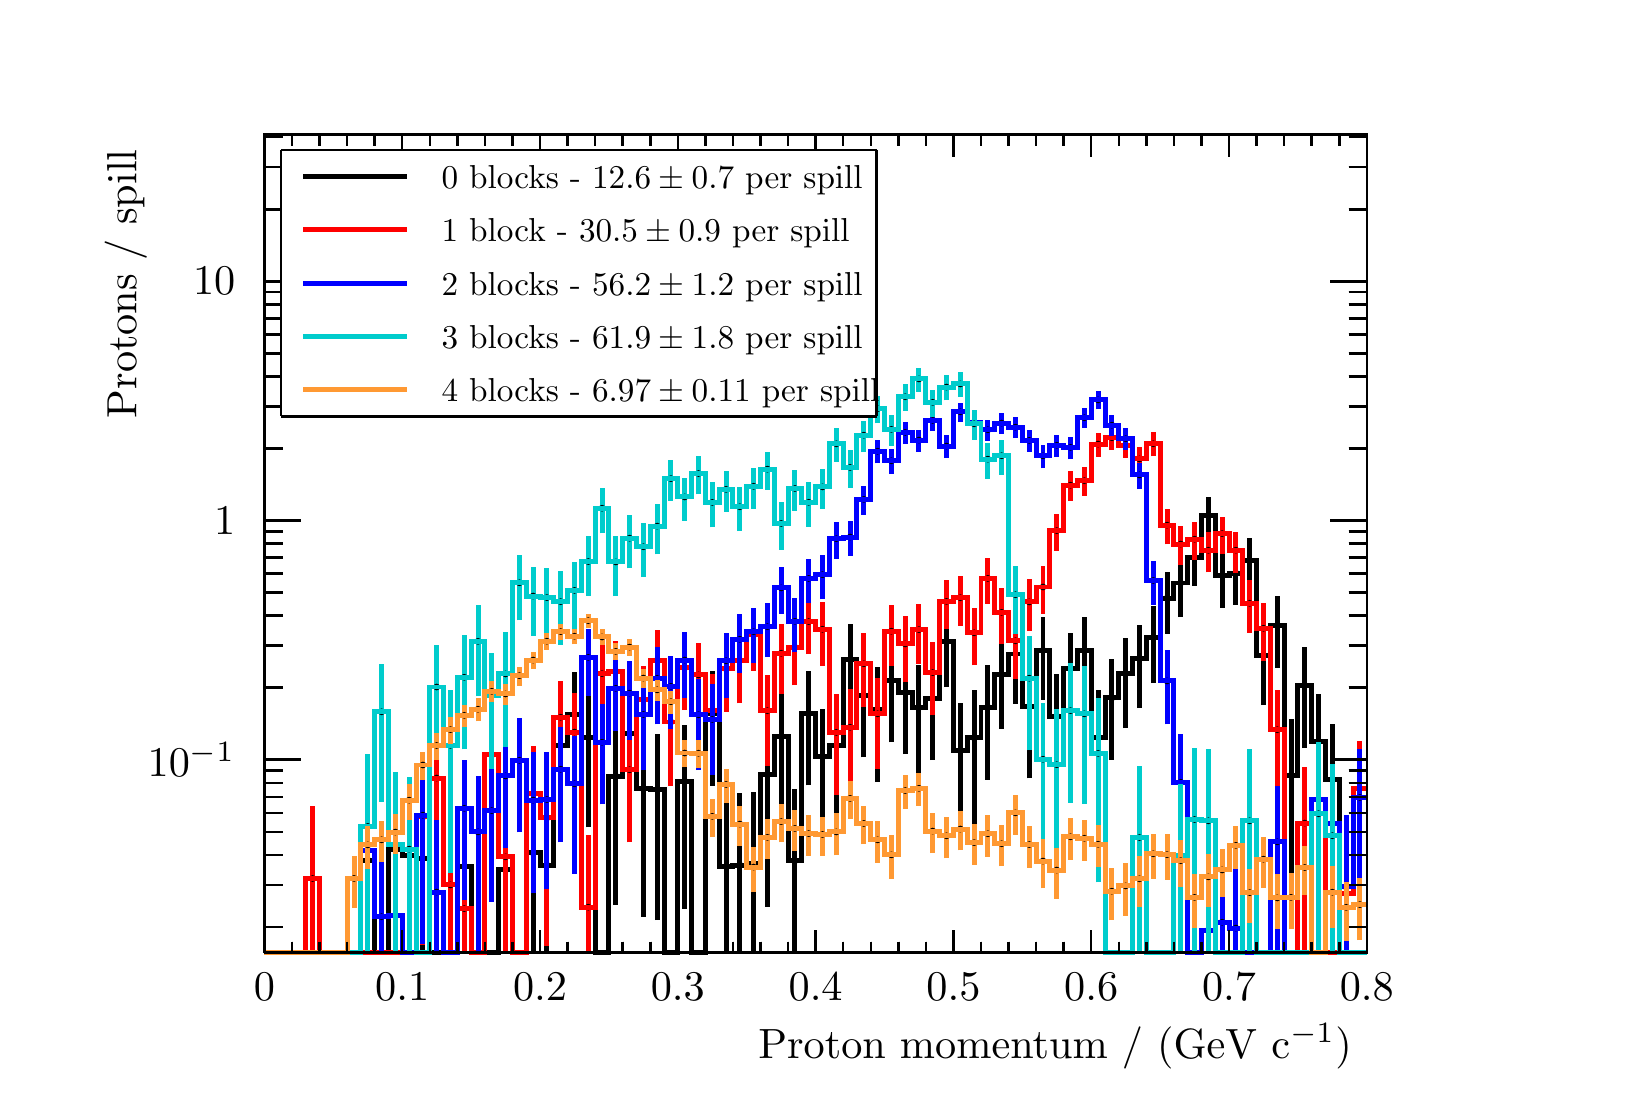
\begin{tikzpicture}
\pgfdeclareplotmark{cross} {
\pgfpathmoveto{\pgfpoint{-0.3\pgfplotmarksize}{\pgfplotmarksize}}
\pgfpathlineto{\pgfpoint{+0.3\pgfplotmarksize}{\pgfplotmarksize}}
\pgfpathlineto{\pgfpoint{+0.3\pgfplotmarksize}{0.3\pgfplotmarksize}}
\pgfpathlineto{\pgfpoint{+1\pgfplotmarksize}{0.3\pgfplotmarksize}}
\pgfpathlineto{\pgfpoint{+1\pgfplotmarksize}{-0.3\pgfplotmarksize}}
\pgfpathlineto{\pgfpoint{+0.3\pgfplotmarksize}{-0.3\pgfplotmarksize}}
\pgfpathlineto{\pgfpoint{+0.3\pgfplotmarksize}{-1.\pgfplotmarksize}}
\pgfpathlineto{\pgfpoint{-0.3\pgfplotmarksize}{-1.\pgfplotmarksize}}
\pgfpathlineto{\pgfpoint{-0.3\pgfplotmarksize}{-0.3\pgfplotmarksize}}
\pgfpathlineto{\pgfpoint{-1.\pgfplotmarksize}{-0.3\pgfplotmarksize}}
\pgfpathlineto{\pgfpoint{-1.\pgfplotmarksize}{0.3\pgfplotmarksize}}
\pgfpathlineto{\pgfpoint{-0.3\pgfplotmarksize}{0.3\pgfplotmarksize}}
\pgfpathclose
\pgfusepathqstroke
}
\pgfdeclareplotmark{cross*} {
\pgfpathmoveto{\pgfpoint{-0.3\pgfplotmarksize}{\pgfplotmarksize}}
\pgfpathlineto{\pgfpoint{+0.3\pgfplotmarksize}{\pgfplotmarksize}}
\pgfpathlineto{\pgfpoint{+0.3\pgfplotmarksize}{0.3\pgfplotmarksize}}
\pgfpathlineto{\pgfpoint{+1\pgfplotmarksize}{0.3\pgfplotmarksize}}
\pgfpathlineto{\pgfpoint{+1\pgfplotmarksize}{-0.3\pgfplotmarksize}}
\pgfpathlineto{\pgfpoint{+0.3\pgfplotmarksize}{-0.3\pgfplotmarksize}}
\pgfpathlineto{\pgfpoint{+0.3\pgfplotmarksize}{-1.\pgfplotmarksize}}
\pgfpathlineto{\pgfpoint{-0.3\pgfplotmarksize}{-1.\pgfplotmarksize}}
\pgfpathlineto{\pgfpoint{-0.3\pgfplotmarksize}{-0.3\pgfplotmarksize}}
\pgfpathlineto{\pgfpoint{-1.\pgfplotmarksize}{-0.3\pgfplotmarksize}}
\pgfpathlineto{\pgfpoint{-1.\pgfplotmarksize}{0.3\pgfplotmarksize}}
\pgfpathlineto{\pgfpoint{-0.3\pgfplotmarksize}{0.3\pgfplotmarksize}}
\pgfpathclose
\pgfusepathqfillstroke
}
\pgfdeclareplotmark{newstar} {
\pgfpathmoveto{\pgfqpoint{0pt}{\pgfplotmarksize}}
\pgfpathlineto{\pgfqpointpolar{44}{0.5\pgfplotmarksize}}
\pgfpathlineto{\pgfqpointpolar{18}{\pgfplotmarksize}}
\pgfpathlineto{\pgfqpointpolar{-20}{0.5\pgfplotmarksize}}
\pgfpathlineto{\pgfqpointpolar{-54}{\pgfplotmarksize}}
\pgfpathlineto{\pgfqpointpolar{-90}{0.5\pgfplotmarksize}}
\pgfpathlineto{\pgfqpointpolar{234}{\pgfplotmarksize}}
\pgfpathlineto{\pgfqpointpolar{198}{0.5\pgfplotmarksize}}
\pgfpathlineto{\pgfqpointpolar{162}{\pgfplotmarksize}}
\pgfpathlineto{\pgfqpointpolar{134}{0.5\pgfplotmarksize}}
\pgfpathclose
\pgfusepathqstroke
}
\pgfdeclareplotmark{newstar*} {
\pgfpathmoveto{\pgfqpoint{0pt}{\pgfplotmarksize}}
\pgfpathlineto{\pgfqpointpolar{44}{0.5\pgfplotmarksize}}
\pgfpathlineto{\pgfqpointpolar{18}{\pgfplotmarksize}}
\pgfpathlineto{\pgfqpointpolar{-20}{0.5\pgfplotmarksize}}
\pgfpathlineto{\pgfqpointpolar{-54}{\pgfplotmarksize}}
\pgfpathlineto{\pgfqpointpolar{-90}{0.5\pgfplotmarksize}}
\pgfpathlineto{\pgfqpointpolar{234}{\pgfplotmarksize}}
\pgfpathlineto{\pgfqpointpolar{198}{0.5\pgfplotmarksize}}
\pgfpathlineto{\pgfqpointpolar{162}{\pgfplotmarksize}}
\pgfpathlineto{\pgfqpointpolar{134}{0.5\pgfplotmarksize}}
\pgfpathclose
\pgfusepathqfillstroke
}
\definecolor{c}{rgb}{1,1,1};
\draw [color=c, fill=c] (0,0) rectangle (20,13.4957);
\draw [color=c, fill=c] (3,1.75444) rectangle (17,12.1461);
\definecolor{c}{rgb}{0,0,0};
\draw [c,line width=0.9] (3,1.75444) -- (3,12.1461) -- (17,12.1461) -- (17,1.75444) -- (3,1.75444);
\definecolor{c}{rgb}{1,1,1};
\draw [color=c, fill=c] (3,1.75444) rectangle (17,12.1461);
\definecolor{c}{rgb}{0,0,0};
\draw [c,line width=0.9] (3,1.75444) -- (3,12.1461) -- (17,12.1461) -- (17,1.75444) -- (3,1.75444);
\draw [c,line width=0.9] (3,1.75444) -- (3.175,1.75444) -- (3.175,1.75444) -- (3.35,1.75444) -- (3.35,1.75444) -- (3.525,1.75444) -- (3.525,1.75444) -- (3.7,1.75444) -- (3.7,1.75444) -- (3.875,1.75444) -- (3.875,1.75444) -- (4.05,1.75444) --
 (4.05,1.75444) -- (4.225,1.75444) -- (4.225,1.75444) -- (4.4,1.75444) -- (4.4,1.75444) -- (4.575,1.75444) -- (4.575,1.75444) -- (4.75,1.75444) -- (4.75,1.75444) -- (4.925,1.75444) -- (4.925,1.75444) -- (5.1,1.75444) -- (5.1,1.75444) --
 (5.275,1.75444) -- (5.275,1.75444) -- (5.45,1.75444) -- (5.45,1.75444) -- (5.625,1.75444) -- (5.625,1.75444) -- (5.8,1.75444) -- (5.8,1.75444) -- (5.975,1.75444) -- (5.975,1.75444) -- (6.15,1.75444) -- (6.15,1.75444) -- (6.325,1.75444) --
 (6.325,1.75444) -- (6.5,1.75444) -- (6.5,1.75444) -- (6.675,1.75444) -- (6.675,1.75444) -- (6.85,1.75444) -- (6.85,1.75444) -- (7.025,1.75444) -- (7.025,1.75444) -- (7.2,1.75444) -- (7.2,1.75444) -- (7.375,1.75444) -- (7.375,1.75444) --
 (7.55,1.75444) -- (7.55,1.75444) -- (7.725,1.75444) -- (7.725,1.75444) -- (7.9,1.75444) -- (7.9,1.75444) -- (8.075,1.75444) -- (8.075,1.75444) -- (8.25,1.75444) -- (8.25,1.75444) -- (8.425,1.75444) -- (8.425,1.75444) -- (8.6,1.75444) --
 (8.6,1.75444) -- (8.775,1.75444) -- (8.775,1.75444) -- (8.95,1.75444) -- (8.95,1.75444) -- (9.125,1.75444) -- (9.125,1.75444) -- (9.3,1.75444) -- (9.3,1.75444) -- (9.475,1.75444) -- (9.475,1.75444) -- (9.65,1.75444) -- (9.65,1.75444) --
 (9.825,1.75444) -- (9.825,1.75444) -- (10,1.75444) -- (10,1.75444) -- (10.175,1.75444) -- (10.175,1.75444) -- (10.35,1.75444) -- (10.35,1.75444) -- (10.525,1.75444) -- (10.525,1.75444) -- (10.7,1.75444) -- (10.7,1.75444) -- (10.875,1.75444) --
 (10.875,1.75444) -- (11.05,1.75444) -- (11.05,1.75444) -- (11.225,1.75444) -- (11.225,1.75444) -- (11.4,1.75444) -- (11.4,1.75444) -- (11.575,1.75444) -- (11.575,1.75444) -- (11.75,1.75444) -- (11.75,1.75444) -- (11.925,1.75444) -- (11.925,1.75444)
 -- (12.1,1.75444) -- (12.1,1.75444) -- (12.275,1.75444) -- (12.275,1.75444) -- (12.45,1.75444) -- (12.45,1.75444) -- (12.625,1.75444) -- (12.625,1.75444) -- (12.8,1.75444) -- (12.8,1.75444) -- (12.975,1.75444) -- (12.975,1.75444) -- (13.15,1.75444)
 -- (13.15,1.75444) -- (13.325,1.75444) -- (13.325,1.75444) -- (13.5,1.75444) -- (13.5,1.75444) -- (13.675,1.75444) -- (13.675,1.75444) -- (13.85,1.75444) -- (13.85,1.75444) -- (14.025,1.75444) -- (14.025,1.75444) -- (14.2,1.75444) -- (14.2,1.75444)
 -- (14.375,1.75444) -- (14.375,1.75444) -- (14.55,1.75444) -- (14.55,1.75444) -- (14.725,1.75444) -- (14.725,1.75444) -- (14.9,1.75444) -- (14.9,1.75444) -- (15.075,1.75444) -- (15.075,1.75444) -- (15.25,1.75444) -- (15.25,1.75444) --
 (15.425,1.75444) -- (15.425,1.75444) -- (15.6,1.75444) -- (15.6,1.75444) -- (15.775,1.75444) -- (15.775,1.75444) -- (15.95,1.75444) -- (15.95,1.75444) -- (16.125,1.75444) -- (16.125,1.75444) -- (16.3,1.75444) -- (16.3,1.75444) -- (16.475,1.75444) --
 (16.475,1.75444) -- (16.65,1.75444) -- (16.65,1.75444) -- (16.825,1.75444) -- (16.825,1.75444) -- (17,1.75444);
\draw [c,line width=0.9] (3,1.75444) -- (17,1.75444);
\draw [c,line width=0.9] (3,2.03785) -- (3,1.75444);
\draw [c,line width=0.9] (3.35,1.89615) -- (3.35,1.75444);
\draw [c,line width=0.9] (3.7,1.89615) -- (3.7,1.75444);
\draw [c,line width=0.9] (4.05,1.89615) -- (4.05,1.75444);
\draw [c,line width=0.9] (4.4,1.89615) -- (4.4,1.75444);
\draw [c,line width=0.9] (4.75,2.03785) -- (4.75,1.75444);
\draw [c,line width=0.9] (5.1,1.89615) -- (5.1,1.75444);
\draw [c,line width=0.9] (5.45,1.89615) -- (5.45,1.75444);
\draw [c,line width=0.9] (5.8,1.89615) -- (5.8,1.75444);
\draw [c,line width=0.9] (6.15,1.89615) -- (6.15,1.75444);
\draw [c,line width=0.9] (6.5,2.03785) -- (6.5,1.75444);
\draw [c,line width=0.9] (6.85,1.89615) -- (6.85,1.75444);
\draw [c,line width=0.9] (7.2,1.89615) -- (7.2,1.75444);
\draw [c,line width=0.9] (7.55,1.89615) -- (7.55,1.75444);
\draw [c,line width=0.9] (7.9,1.89615) -- (7.9,1.75444);
\draw [c,line width=0.9] (8.25,2.03785) -- (8.25,1.75444);
\draw [c,line width=0.9] (8.6,1.89615) -- (8.6,1.75444);
\draw [c,line width=0.9] (8.95,1.89615) -- (8.95,1.75444);
\draw [c,line width=0.9] (9.3,1.89615) -- (9.3,1.75444);
\draw [c,line width=0.9] (9.65,1.89615) -- (9.65,1.75444);
\draw [c,line width=0.9] (10,2.03785) -- (10,1.75444);
\draw [c,line width=0.9] (10.35,1.89615) -- (10.35,1.75444);
\draw [c,line width=0.9] (10.7,1.89615) -- (10.7,1.75444);
\draw [c,line width=0.9] (11.05,1.89615) -- (11.05,1.75444);
\draw [c,line width=0.9] (11.4,1.89615) -- (11.4,1.75444);
\draw [c,line width=0.9] (11.75,2.03785) -- (11.75,1.75444);
\draw [c,line width=0.9] (12.1,1.89615) -- (12.1,1.75444);
\draw [c,line width=0.9] (12.45,1.89615) -- (12.45,1.75444);
\draw [c,line width=0.9] (12.8,1.89615) -- (12.8,1.75444);
\draw [c,line width=0.9] (13.15,1.89615) -- (13.15,1.75444);
\draw [c,line width=0.9] (13.5,2.03785) -- (13.5,1.75444);
\draw [c,line width=0.9] (13.85,1.89615) -- (13.85,1.75444);
\draw [c,line width=0.9] (14.2,1.89615) -- (14.2,1.75444);
\draw [c,line width=0.9] (14.55,1.89615) -- (14.55,1.75444);
\draw [c,line width=0.9] (14.9,1.89615) -- (14.9,1.75444);
\draw [c,line width=0.9] (15.25,2.03785) -- (15.25,1.75444);
\draw [c,line width=0.9] (15.6,1.89615) -- (15.6,1.75444);
\draw [c,line width=0.9] (15.95,1.89615) -- (15.95,1.75444);
\draw [c,line width=0.9] (16.3,1.89615) -- (16.3,1.75444);
\draw [c,line width=0.9] (16.65,1.89615) -- (16.65,1.75444);
\draw [c,line width=0.9] (17,2.03785) -- (17,1.75444);
\draw [anchor=base] (3,1.14713) node[scale=1.52731, color=c, rotate=0]{0};
\draw [anchor=base] (4.75,1.14713) node[scale=1.52731, color=c, rotate=0]{0.1};
\draw [anchor=base] (6.5,1.14713) node[scale=1.52731, color=c, rotate=0]{0.2};
\draw [anchor=base] (8.25,1.14713) node[scale=1.52731, color=c, rotate=0]{0.3};
\draw [anchor=base] (10,1.14713) node[scale=1.52731, color=c, rotate=0]{0.4};
\draw [anchor=base] (11.75,1.14713) node[scale=1.52731, color=c, rotate=0]{0.5};
\draw [anchor=base] (13.5,1.14713) node[scale=1.52731, color=c, rotate=0]{0.6};
\draw [anchor=base] (15.25,1.14713) node[scale=1.52731, color=c, rotate=0]{0.7};
\draw [anchor=base] (17,1.14713) node[scale=1.52731, color=c, rotate=0]{0.8};
\draw [anchor= east] (17,0.566819) node[scale=1.52731, color=c, rotate=0]{Proton momentum / (GeV c$^{-1}$)};
\draw [c,line width=0.9] (3,12.1461) -- (17,12.1461);
\draw [c,line width=0.9] (3,11.8627) -- (3,12.1461);
\draw [c,line width=0.9] (3.35,12.0044) -- (3.35,12.1461);
\draw [c,line width=0.9] (3.7,12.0044) -- (3.7,12.1461);
\draw [c,line width=0.9] (4.05,12.0044) -- (4.05,12.1461);
\draw [c,line width=0.9] (4.4,12.0044) -- (4.4,12.1461);
\draw [c,line width=0.9] (4.75,11.8627) -- (4.75,12.1461);
\draw [c,line width=0.9] (5.1,12.0044) -- (5.1,12.1461);
\draw [c,line width=0.9] (5.45,12.0044) -- (5.45,12.1461);
\draw [c,line width=0.9] (5.8,12.0044) -- (5.8,12.1461);
\draw [c,line width=0.9] (6.15,12.0044) -- (6.15,12.1461);
\draw [c,line width=0.9] (6.5,11.8627) -- (6.5,12.1461);
\draw [c,line width=0.9] (6.85,12.0044) -- (6.85,12.1461);
\draw [c,line width=0.9] (7.2,12.0044) -- (7.2,12.1461);
\draw [c,line width=0.9] (7.55,12.0044) -- (7.55,12.1461);
\draw [c,line width=0.9] (7.9,12.0044) -- (7.9,12.1461);
\draw [c,line width=0.9] (8.25,11.8627) -- (8.25,12.1461);
\draw [c,line width=0.9] (8.6,12.0044) -- (8.6,12.1461);
\draw [c,line width=0.9] (8.95,12.0044) -- (8.95,12.1461);
\draw [c,line width=0.9] (9.3,12.0044) -- (9.3,12.1461);
\draw [c,line width=0.9] (9.65,12.0044) -- (9.65,12.1461);
\draw [c,line width=0.9] (10,11.8627) -- (10,12.1461);
\draw [c,line width=0.9] (10.35,12.0044) -- (10.35,12.1461);
\draw [c,line width=0.9] (10.7,12.0044) -- (10.7,12.1461);
\draw [c,line width=0.9] (11.05,12.0044) -- (11.05,12.1461);
\draw [c,line width=0.9] (11.4,12.0044) -- (11.4,12.1461);
\draw [c,line width=0.9] (11.75,11.8627) -- (11.75,12.1461);
\draw [c,line width=0.9] (12.1,12.0044) -- (12.1,12.1461);
\draw [c,line width=0.9] (12.45,12.0044) -- (12.45,12.1461);
\draw [c,line width=0.9] (12.8,12.0044) -- (12.8,12.1461);
\draw [c,line width=0.9] (13.15,12.0044) -- (13.15,12.1461);
\draw [c,line width=0.9] (13.5,11.8627) -- (13.5,12.1461);
\draw [c,line width=0.9] (13.85,12.0044) -- (13.85,12.1461);
\draw [c,line width=0.9] (14.2,12.0044) -- (14.2,12.1461);
\draw [c,line width=0.9] (14.55,12.0044) -- (14.55,12.1461);
\draw [c,line width=0.9] (14.9,12.0044) -- (14.9,12.1461);
\draw [c,line width=0.9] (15.25,11.8627) -- (15.25,12.1461);
\draw [c,line width=0.9] (15.6,12.0044) -- (15.6,12.1461);
\draw [c,line width=0.9] (15.95,12.0044) -- (15.95,12.1461);
\draw [c,line width=0.9] (16.3,12.0044) -- (16.3,12.1461);
\draw [c,line width=0.9] (16.65,12.0044) -- (16.65,12.1461);
\draw [c,line width=0.9] (17,11.8627) -- (17,12.1461);
\draw [c,line width=0.9] (3,1.75444) -- (3,12.1461);
\draw [c,line width=0.9] (3.231,2.08178) -- (3,2.08178);
\draw [c,line width=0.9] (3.231,2.61678) -- (3,2.61678);
\draw [c,line width=0.9] (3.231,2.99637) -- (3,2.99637);
\draw [c,line width=0.9] (3.231,3.29081) -- (3,3.29081);
\draw [c,line width=0.9] (3.231,3.53138) -- (3,3.53138);
\draw [c,line width=0.9] (3.231,3.73478) -- (3,3.73478);
\draw [c,line width=0.9] (3.231,3.91097) -- (3,3.91097);
\draw [c,line width=0.9] (3.231,4.06638) -- (3,4.06638);
\draw [c,line width=0.9] (3.462,4.2054) -- (3,4.2054);
\draw [anchor= east] (2.82,4.2054) node[scale=1.52731, color=c, rotate=0]{$10^{-1}$};
\draw [c,line width=0.9] (3.231,5.12) -- (3,5.12);
\draw [c,line width=0.9] (3.231,5.655) -- (3,5.655);
\draw [c,line width=0.9] (3.231,6.03459) -- (3,6.03459);
\draw [c,line width=0.9] (3.231,6.32902) -- (3,6.32902);
\draw [c,line width=0.9] (3.231,6.56959) -- (3,6.56959);
\draw [c,line width=0.9] (3.231,6.77299) -- (3,6.77299);
\draw [c,line width=0.9] (3.231,6.94918) -- (3,6.94918);
\draw [c,line width=0.9] (3.231,7.1046) -- (3,7.1046);
\draw [c,line width=0.9] (3.462,7.24362) -- (3,7.24362);
\draw [anchor= east] (2.82,7.24362) node[scale=1.52731, color=c, rotate=0]{1};
\draw [c,line width=0.9] (3.231,8.15821) -- (3,8.15821);
\draw [c,line width=0.9] (3.231,8.69321) -- (3,8.69321);
\draw [c,line width=0.9] (3.231,9.07281) -- (3,9.07281);
\draw [c,line width=0.9] (3.231,9.36724) -- (3,9.36724);
\draw [c,line width=0.9] (3.231,9.60781) -- (3,9.60781);
\draw [c,line width=0.9] (3.231,9.81121) -- (3,9.81121);
\draw [c,line width=0.9] (3.231,9.9874) -- (3,9.9874);
\draw [c,line width=0.9] (3.231,10.1428) -- (3,10.1428);
\draw [c,line width=0.9] (3.462,10.2818) -- (3,10.2818);
\draw [anchor= east] (2.82,10.2818) node[scale=1.52731, color=c, rotate=0]{10};
\draw [c,line width=0.9] (3.231,11.1964) -- (3,11.1964);
\draw [c,line width=0.9] (3.231,11.7314) -- (3,11.7314);
\draw [c,line width=0.9] (3.231,12.111) -- (3,12.111);
\draw [anchor= east] (1.24,12.1461) node[scale=1.52731, color=c, rotate=90]{Protons / spill};
\draw [c,line width=0.9] (17,1.75444) -- (17,12.1461);
\draw [c,line width=0.9] (16.769,2.08178) -- (17,2.08178);
\draw [c,line width=0.9] (16.769,2.61678) -- (17,2.61678);
\draw [c,line width=0.9] (16.769,2.99637) -- (17,2.99637);
\draw [c,line width=0.9] (16.769,3.29081) -- (17,3.29081);
\draw [c,line width=0.9] (16.769,3.53138) -- (17,3.53138);
\draw [c,line width=0.9] (16.769,3.73478) -- (17,3.73478);
\draw [c,line width=0.9] (16.769,3.91097) -- (17,3.91097);
\draw [c,line width=0.9] (16.769,4.06638) -- (17,4.06638);
\draw [c,line width=0.9] (16.538,4.2054) -- (17,4.2054);
\draw [c,line width=0.9] (16.769,5.12) -- (17,5.12);
\draw [c,line width=0.9] (16.769,5.655) -- (17,5.655);
\draw [c,line width=0.9] (16.769,6.03459) -- (17,6.03459);
\draw [c,line width=0.9] (16.769,6.32902) -- (17,6.32902);
\draw [c,line width=0.9] (16.769,6.56959) -- (17,6.56959);
\draw [c,line width=0.9] (16.769,6.77299) -- (17,6.77299);
\draw [c,line width=0.9] (16.769,6.94918) -- (17,6.94918);
\draw [c,line width=0.9] (16.769,7.1046) -- (17,7.1046);
\draw [c,line width=0.9] (16.538,7.24362) -- (17,7.24362);
\draw [c,line width=0.9] (16.769,8.15821) -- (17,8.15821);
\draw [c,line width=0.9] (16.769,8.69321) -- (17,8.69321);
\draw [c,line width=0.9] (16.769,9.07281) -- (17,9.07281);
\draw [c,line width=0.9] (16.769,9.36724) -- (17,9.36724);
\draw [c,line width=0.9] (16.769,9.60781) -- (17,9.60781);
\draw [c,line width=0.9] (16.769,9.81121) -- (17,9.81121);
\draw [c,line width=0.9] (16.769,9.9874) -- (17,9.9874);
\draw [c,line width=0.9] (16.769,10.1428) -- (17,10.1428);
\draw [c,line width=0.9] (16.538,10.2818) -- (17,10.2818);
\draw [c,line width=0.9] (16.769,11.1964) -- (17,11.1964);
\draw [c,line width=0.9] (16.769,11.7314) -- (17,11.7314);
\draw [c,line width=0.9] (16.769,12.111) -- (17,12.111);
\draw [c,line width=1.8] (4.3125,1.75444) -- (4.3125,2.93093);
\draw [c,line width=1.8] (4.3125,2.93093) -- (4.3125,3.84552);
\foreach \P in {(4.3125,2.93093)}{\draw[mark options={color=c,fill=c},mark size=2.402402pt,mark=*,mark size=1pt] plot coordinates {\P};}
\draw [c,line width=1.8] (4.6625,1.75444) -- (4.6625,3.07155);
\draw [c,line width=1.8] (4.6625,3.07155) -- (4.6625,3.98615);
\foreach \P in {(4.6625,3.07155)}{\draw[mark options={color=c,fill=c},mark size=2.402402pt,mark=*,mark size=1pt] plot coordinates {\P};}
\draw [c,line width=1.8] (4.8375,1.75444) -- (4.8375,2.99212);
\draw [c,line width=1.8] (4.8375,2.99212) -- (4.8375,3.90672);
\foreach \P in {(4.8375,2.99212)}{\draw[mark options={color=c,fill=c},mark size=2.402402pt,mark=*,mark size=1pt] plot coordinates {\P};}
\draw [c,line width=1.8] (5.0125,1.75444) -- (5.0125,2.95413);
\draw [c,line width=1.8] (5.0125,2.95413) -- (5.0125,3.86872);
\foreach \P in {(5.0125,2.95413)}{\draw[mark options={color=c,fill=c},mark size=2.402402pt,mark=*,mark size=1pt] plot coordinates {\P};}
\draw [c,line width=1.8] (5.5375,1.75444) -- (5.5375,2.85063);
\draw [c,line width=1.8] (5.5375,2.85063) -- (5.5375,3.76522);
\foreach \P in {(5.5375,2.85063)}{\draw[mark options={color=c,fill=c},mark size=2.402402pt,mark=*,mark size=1pt] plot coordinates {\P};}
\draw [c,line width=1.8] (6.0625,1.75444) -- (6.0625,2.80804);
\draw [c,line width=1.8] (6.0625,2.80804) -- (6.0625,3.72264);
\foreach \P in {(6.0625,2.80804)}{\draw[mark options={color=c,fill=c},mark size=2.402402pt,mark=*,mark size=1pt] plot coordinates {\P};}
\draw [c,line width=1.8] (6.4125,1.75444) -- (6.4125,3.02135);
\draw [c,line width=1.8] (6.4125,3.02135) -- (6.4125,3.93595);
\foreach \P in {(6.4125,3.02135)}{\draw[mark options={color=c,fill=c},mark size=2.402402pt,mark=*,mark size=1pt] plot coordinates {\P};}
\draw [c,line width=1.8] (6.5875,1.75444) -- (6.5875,2.86805);
\draw [c,line width=1.8] (6.5875,2.86805) -- (6.5875,3.78265);
\foreach \P in {(6.5875,2.86805)}{\draw[mark options={color=c,fill=c},mark size=2.402402pt,mark=*,mark size=1pt] plot coordinates {\P};}
\draw [c,line width=1.8] (6.7625,3.25045) -- (6.7625,4.38708);
\draw [c,line width=1.8] (6.7625,4.38708) -- (6.7625,4.9885);
\foreach \P in {(6.7625,4.38708)}{\draw[mark options={color=c,fill=c},mark size=2.402402pt,mark=*,mark size=1pt] plot coordinates {\P};}
\draw [c,line width=1.8] (6.9375,3.86542) -- (6.9375,4.78232);
\draw [c,line width=1.8] (6.9375,4.78232) -- (6.9375,5.31809);
\foreach \P in {(6.9375,4.78232)}{\draw[mark options={color=c,fill=c},mark size=2.402402pt,mark=*,mark size=1pt] plot coordinates {\P};}
\draw [c,line width=1.8] (7.1125,3.34711) -- (7.1125,4.4855);
\draw [c,line width=1.8] (7.1125,4.4855) -- (7.1125,5.08739);
\foreach \P in {(7.1125,4.4855)}{\draw[mark options={color=c,fill=c},mark size=2.402402pt,mark=*,mark size=1pt] plot coordinates {\P};}
\draw [c,line width=1.8] (7.4625,2.36048) -- (7.4625,3.99755);
\draw [c,line width=1.8] (7.4625,3.99755) -- (7.4625,4.70607);
\foreach \P in {(7.4625,3.99755)}{\draw[mark options={color=c,fill=c},mark size=2.402402pt,mark=*,mark size=1pt] plot coordinates {\P};}
\draw [c,line width=1.8] (7.6375,3.38215) -- (7.6375,4.53369);
\draw [c,line width=1.8] (7.6375,4.53369) -- (7.6375,5.13907);
\foreach \P in {(7.6375,4.53369)}{\draw[mark options={color=c,fill=c},mark size=2.402402pt,mark=*,mark size=1pt] plot coordinates {\P};}
\draw [c,line width=1.8] (7.8125,2.21378) -- (7.8125,3.83427);
\draw [c,line width=1.8] (7.8125,3.83427) -- (7.8125,4.53996);
\foreach \P in {(7.8125,3.83427)}{\draw[mark options={color=c,fill=c},mark size=2.402402pt,mark=*,mark size=1pt] plot coordinates {\P};}
\draw [c,line width=1.8] (7.9875,2.16943) -- (7.9875,3.82634);
\draw [c,line width=1.8] (7.9875,3.82634) -- (7.9875,4.53818);
\foreach \P in {(7.9875,3.82634)}{\draw[mark options={color=c,fill=c},mark size=2.402402pt,mark=*,mark size=1pt] plot coordinates {\P};}
\draw [c,line width=1.8] (8.3375,2.31014) -- (8.3375,3.93412);
\draw [c,line width=1.8] (8.3375,3.93412) -- (8.3375,4.64041);
\foreach \P in {(8.3375,3.93412)}{\draw[mark options={color=c,fill=c},mark size=2.402402pt,mark=*,mark size=1pt] plot coordinates {\P};}
\draw [c,line width=1.8] (8.6875,3.87377) -- (8.6875,4.79496);
\draw [c,line width=1.8] (8.6875,4.79496) -- (8.6875,5.33215);
\foreach \P in {(8.6875,4.79496)}{\draw[mark options={color=c,fill=c},mark size=2.402402pt,mark=*,mark size=1pt] plot coordinates {\P};}
\draw [c,line width=1.8] (8.8625,1.75444) -- (8.8625,2.85063);
\draw [c,line width=1.8] (8.8625,2.85063) -- (8.8625,3.76522);
\foreach \P in {(8.8625,2.85063)}{\draw[mark options={color=c,fill=c},mark size=2.402402pt,mark=*,mark size=1pt] plot coordinates {\P};}
\draw [c,line width=1.8] (9.0375,1.75444) -- (9.0375,2.86805);
\draw [c,line width=1.8] (9.0375,2.86805) -- (9.0375,3.78265);
\foreach \P in {(9.0375,2.86805)}{\draw[mark options={color=c,fill=c},mark size=2.402402pt,mark=*,mark size=1pt] plot coordinates {\P};}
\draw [c,line width=1.8] (9.2125,1.75444) -- (9.2125,2.88572);
\draw [c,line width=1.8] (9.2125,2.88572) -- (9.2125,3.80031);
\foreach \P in {(9.2125,2.88572)}{\draw[mark options={color=c,fill=c},mark size=2.402402pt,mark=*,mark size=1pt] plot coordinates {\P};}
\draw [c,line width=1.8] (9.3875,2.33881) -- (9.3875,4.0146);
\draw [c,line width=1.8] (9.3875,4.0146) -- (9.3875,4.72955);
\foreach \P in {(9.3875,4.0146)}{\draw[mark options={color=c,fill=c},mark size=2.402402pt,mark=*,mark size=1pt] plot coordinates {\P};}
\draw [c,line width=1.8] (9.5625,3.34321) -- (9.5625,4.49958);
\draw [c,line width=1.8] (9.5625,4.49958) -- (9.5625,5.10624);
\foreach \P in {(9.5625,4.49958)}{\draw[mark options={color=c,fill=c},mark size=2.402402pt,mark=*,mark size=1pt] plot coordinates {\P};}
\draw [c,line width=1.8] (9.7375,1.75444) -- (9.7375,2.92176);
\draw [c,line width=1.8] (9.7375,2.92176) -- (9.7375,3.83636);
\foreach \P in {(9.7375,2.92176)}{\draw[mark options={color=c,fill=c},mark size=2.402402pt,mark=*,mark size=1pt] plot coordinates {\P};}
\draw [c,line width=1.8] (9.9125,3.87847) -- (9.9125,4.7945);
\draw [c,line width=1.8] (9.9125,4.7945) -- (9.9125,5.32998);
\foreach \P in {(9.9125,4.7945)}{\draw[mark options={color=c,fill=c},mark size=2.402402pt,mark=*,mark size=1pt] plot coordinates {\P};}
\draw [c,line width=1.8] (10.0875,3.10627) -- (10.0875,4.24319);
\draw [c,line width=1.8] (10.0875,4.24319) -- (10.0875,4.84469);
\foreach \P in {(10.0875,4.24319)}{\draw[mark options={color=c,fill=c},mark size=2.402402pt,mark=*,mark size=1pt] plot coordinates {\P};}
\draw [c,line width=1.8] (10.2625,3.25095) -- (10.2625,4.38854);
\draw [c,line width=1.8] (10.2625,4.38854) -- (10.2625,4.99022);
\foreach \P in {(10.2625,4.38854)}{\draw[mark options={color=c,fill=c},mark size=2.402402pt,mark=*,mark size=1pt] plot coordinates {\P};}
\draw [c,line width=1.8] (10.4375,4.77751) -- (10.4375,5.47555);
\draw [c,line width=1.8] (10.4375,5.47555) -- (10.4375,5.92968);
\foreach \P in {(10.4375,5.47555)}{\draw[mark options={color=c,fill=c},mark size=2.402402pt,mark=*,mark size=1pt] plot coordinates {\P};}
\draw [c,line width=1.8] (10.6125,4.23455) -- (10.6125,5.01943);
\draw [c,line width=1.8] (10.6125,5.01943) -- (10.6125,5.50819);
\foreach \P in {(10.6125,5.01943)}{\draw[mark options={color=c,fill=c},mark size=2.402402pt,mark=*,mark size=1pt] plot coordinates {\P};}
\draw [c,line width=1.8] (10.7875,3.92071) -- (10.7875,4.84054);
\draw [c,line width=1.8] (10.7875,4.84054) -- (10.7875,5.37728);
\foreach \P in {(10.7875,4.84054)}{\draw[mark options={color=c,fill=c},mark size=2.402402pt,mark=*,mark size=1pt] plot coordinates {\P};}
\draw [c,line width=1.8] (10.9625,4.42626) -- (10.9625,5.21609);
\draw [c,line width=1.8] (10.9625,5.21609) -- (10.9625,5.70673);
\foreach \P in {(10.9625,5.21609)}{\draw[mark options={color=c,fill=c},mark size=2.402402pt,mark=*,mark size=1pt] plot coordinates {\P};}
\draw [c,line width=1.8] (11.1375,4.2755) -- (11.1375,5.06242);
\draw [c,line width=1.8] (11.1375,5.06242) -- (11.1375,5.55196);
\foreach \P in {(11.1375,5.06242)}{\draw[mark options={color=c,fill=c},mark size=2.402402pt,mark=*,mark size=1pt] plot coordinates {\P};}
\draw [c,line width=1.8] (11.3125,3.95275) -- (11.3125,4.86925);
\draw [c,line width=1.8] (11.3125,4.86925) -- (11.3125,5.4049);
\foreach \P in {(11.3125,4.86925)}{\draw[mark options={color=c,fill=c},mark size=2.402402pt,mark=*,mark size=1pt] plot coordinates {\P};}
\draw [c,line width=1.8] (11.4875,4.20095) -- (11.4875,4.98627);
\draw [c,line width=1.8] (11.4875,4.98627) -- (11.4875,5.47521);
\foreach \P in {(11.4875,4.98627)}{\draw[mark options={color=c,fill=c},mark size=2.402402pt,mark=*,mark size=1pt] plot coordinates {\P};}
\draw [c,line width=1.8] (11.6625,5.12769) -- (11.6625,5.70585);
\draw [c,line width=1.8] (11.6625,5.70585) -- (11.6625,6.1065);
\foreach \P in {(11.6625,5.70585)}{\draw[mark options={color=c,fill=c},mark size=2.402402pt,mark=*,mark size=1pt] plot coordinates {\P};}
\draw [c,line width=1.8] (11.8375,3.17468) -- (11.8375,4.32068);
\draw [c,line width=1.8] (11.8375,4.32068) -- (11.8375,4.92461);
\foreach \P in {(11.8375,4.32068)}{\draw[mark options={color=c,fill=c},mark size=2.402402pt,mark=*,mark size=1pt] plot coordinates {\P};}
\draw [c,line width=1.8] (12.0125,3.32874) -- (12.0125,4.48452);
\draw [c,line width=1.8] (12.0125,4.48452) -- (12.0125,5.09102);
\foreach \P in {(12.0125,4.48452)}{\draw[mark options={color=c,fill=c},mark size=2.402402pt,mark=*,mark size=1pt] plot coordinates {\P};}
\draw [c,line width=1.8] (12.1875,3.95327) -- (12.1875,4.87297);
\draw [c,line width=1.8] (12.1875,4.87297) -- (12.1875,5.40968);
\foreach \P in {(12.1875,4.87297)}{\draw[mark options={color=c,fill=c},mark size=2.402402pt,mark=*,mark size=1pt] plot coordinates {\P};}
\draw [c,line width=1.8] (12.3625,4.59718) -- (12.3625,5.29013);
\draw [c,line width=1.8] (12.3625,5.29013) -- (12.3625,5.74213);
\foreach \P in {(12.3625,5.29013)}{\draw[mark options={color=c,fill=c},mark size=2.402402pt,mark=*,mark size=1pt] plot coordinates {\P};}
\draw [c,line width=1.8] (12.5375,4.91642) -- (12.5375,5.54822);
\draw [c,line width=1.8] (12.5375,5.54822) -- (12.5375,5.97368);
\foreach \P in {(12.5375,5.54822)}{\draw[mark options={color=c,fill=c},mark size=2.402402pt,mark=*,mark size=1pt] plot coordinates {\P};}
\draw [c,line width=1.8] (12.7125,3.96764) -- (12.7125,4.88277);
\draw [c,line width=1.8] (12.7125,4.88277) -- (12.7125,5.41796);
\foreach \P in {(12.7125,4.88277)}{\draw[mark options={color=c,fill=c},mark size=2.402402pt,mark=*,mark size=1pt] plot coordinates {\P};}
\draw [c,line width=1.8] (12.8875,4.96455) -- (12.8875,5.59468);
\draw [c,line width=1.8] (12.8875,5.59468) -- (12.8875,6.01939);
\foreach \P in {(12.8875,5.59468)}{\draw[mark options={color=c,fill=c},mark size=2.402402pt,mark=*,mark size=1pt] plot coordinates {\P};}
\draw [c,line width=1.8] (13.0625,3.84251) -- (13.0625,4.75854);
\draw [c,line width=1.8] (13.0625,4.75854) -- (13.0625,5.29402);
\foreach \P in {(13.0625,4.75854)}{\draw[mark options={color=c,fill=c},mark size=2.402402pt,mark=*,mark size=1pt] plot coordinates {\P};}
\draw [c,line width=1.8] (13.2375,4.67069) -- (13.2375,5.3639);
\draw [c,line width=1.8] (13.2375,5.3639) -- (13.2375,5.816);
\foreach \P in {(13.2375,5.3639)}{\draw[mark options={color=c,fill=c},mark size=2.402402pt,mark=*,mark size=1pt] plot coordinates {\P};}
\draw [c,line width=1.8] (13.4125,4.96155) -- (13.4125,5.59277);
\draw [c,line width=1.8] (13.4125,5.59277) -- (13.4125,6.01796);
\foreach \P in {(13.4125,5.59277)}{\draw[mark options={color=c,fill=c},mark size=2.402402pt,mark=*,mark size=1pt] plot coordinates {\P};}
\draw [c,line width=1.8] (13.5875,3.34164) -- (13.5875,4.48746);
\draw [c,line width=1.8] (13.5875,4.48746) -- (13.5875,5.09134);
\foreach \P in {(13.5875,4.48746)}{\draw[mark options={color=c,fill=c},mark size=2.402402pt,mark=*,mark size=1pt] plot coordinates {\P};}
\draw [c,line width=1.8] (13.7625,4.19998) -- (13.7625,4.98996);
\draw [c,line width=1.8] (13.7625,4.98996) -- (13.7625,5.48067);
\foreach \P in {(13.7625,4.98996)}{\draw[mark options={color=c,fill=c},mark size=2.402402pt,mark=*,mark size=1pt] plot coordinates {\P};}
\draw [c,line width=1.8] (13.9375,4.60775) -- (13.9375,5.30103);
\draw [c,line width=1.8] (13.9375,5.30103) -- (13.9375,5.75317);
\foreach \P in {(13.9375,5.30103)}{\draw[mark options={color=c,fill=c},mark size=2.402402pt,mark=*,mark size=1pt] plot coordinates {\P};}
\draw [c,line width=1.8] (14.1125,4.86217) -- (14.1125,5.49368);
\draw [c,line width=1.8] (14.1125,5.49368) -- (14.1125,5.919);
\foreach \P in {(14.1125,5.49368)}{\draw[mark options={color=c,fill=c},mark size=2.402402pt,mark=*,mark size=1pt] plot coordinates {\P};}
\draw [c,line width=1.8] (14.2875,5.17753) -- (14.2875,5.7555);
\draw [c,line width=1.8] (14.2875,5.7555) -- (14.2875,6.15606);
\foreach \P in {(14.2875,5.7555)}{\draw[mark options={color=c,fill=c},mark size=2.402402pt,mark=*,mark size=1pt] plot coordinates {\P};}
\draw [c,line width=1.8] (14.4625,5.80529) -- (14.4625,6.25782);
\draw [c,line width=1.8] (14.4625,6.25782) -- (14.4625,6.59415);
\foreach \P in {(14.4625,6.25782)}{\draw[mark options={color=c,fill=c},mark size=2.402402pt,mark=*,mark size=1pt] plot coordinates {\P};}
\draw [c,line width=1.8] (14.6375,6.0176) -- (14.6375,6.44992);
\draw [c,line width=1.8] (14.6375,6.44992) -- (14.6375,6.775);
\foreach \P in {(14.6375,6.44992)}{\draw[mark options={color=c,fill=c},mark size=2.402402pt,mark=*,mark size=1pt] plot coordinates {\P};}
\draw [c,line width=1.8] (14.8125,6.41599) -- (14.8125,6.77286);
\draw [c,line width=1.8] (14.8125,6.77286) -- (14.8125,7.05347);
\foreach \P in {(14.8125,6.77286)}{\draw[mark options={color=c,fill=c},mark size=2.402402pt,mark=*,mark size=1pt] plot coordinates {\P};}
\draw [c,line width=1.8] (14.9875,7.01185) -- (14.9875,7.30142);
\draw [c,line width=1.8] (14.9875,7.30142) -- (14.9875,7.53874);
\foreach \P in {(14.9875,7.30142)}{\draw[mark options={color=c,fill=c},mark size=2.402402pt,mark=*,mark size=1pt] plot coordinates {\P};}
\draw [c,line width=1.8] (15.1625,6.13347) -- (15.1625,6.54653);
\draw [c,line width=1.8] (15.1625,6.54653) -- (15.1625,6.86064);
\foreach \P in {(15.1625,6.54653)}{\draw[mark options={color=c,fill=c},mark size=2.402402pt,mark=*,mark size=1pt] plot coordinates {\P};}
\draw [c,line width=1.8] (15.3375,6.17694) -- (15.3375,6.57387);
\draw [c,line width=1.8] (15.3375,6.57387) -- (15.3375,6.87859);
\foreach \P in {(15.3375,6.57387)}{\draw[mark options={color=c,fill=c},mark size=2.402402pt,mark=*,mark size=1pt] plot coordinates {\P};}
\draw [c,line width=1.8] (15.5125,6.36689) -- (15.5125,6.7354);
\draw [c,line width=1.8] (15.5125,6.7354) -- (15.5125,7.02314);
\foreach \P in {(15.5125,6.7354)}{\draw[mark options={color=c,fill=c},mark size=2.402402pt,mark=*,mark size=1pt] plot coordinates {\P};}
\draw [c,line width=1.8] (15.6875,4.89982) -- (15.6875,5.53131);
\draw [c,line width=1.8] (15.6875,5.53131) -- (15.6875,5.95663);
\foreach \P in {(15.6875,5.53131)}{\draw[mark options={color=c,fill=c},mark size=2.402402pt,mark=*,mark size=1pt] plot coordinates {\P};}
\draw [c,line width=1.8] (15.8625,5.37131) -- (15.8625,5.90821);
\draw [c,line width=1.8] (15.8625,5.90821) -- (15.8625,6.28875);
\foreach \P in {(15.8625,5.90821)}{\draw[mark options={color=c,fill=c},mark size=2.402402pt,mark=*,mark size=1pt] plot coordinates {\P};}
\draw [c,line width=1.8] (16.0375,2.34294) -- (16.0375,4.00897);
\draw [c,line width=1.8] (16.0375,4.00897) -- (16.0375,4.72232);
\foreach \P in {(16.0375,4.00897)}{\draw[mark options={color=c,fill=c},mark size=2.402402pt,mark=*,mark size=1pt] plot coordinates {\P};}
\draw [c,line width=1.8] (16.2125,4.35306) -- (16.2125,5.14747);
\draw [c,line width=1.8] (16.2125,5.14747) -- (16.2125,5.63985);
\foreach \P in {(16.2125,5.14747)}{\draw[mark options={color=c,fill=c},mark size=2.402402pt,mark=*,mark size=1pt] plot coordinates {\P};}
\draw [c,line width=1.8] (16.3875,3.29584) -- (16.3875,4.43847);
\draw [c,line width=1.8] (16.3875,4.43847) -- (16.3875,5.0415);
\foreach \P in {(16.3875,4.43847)}{\draw[mark options={color=c,fill=c},mark size=2.402402pt,mark=*,mark size=1pt] plot coordinates {\P};}
\draw [c,line width=1.8] (16.5625,2.33055) -- (16.5625,3.95081);
\draw [c,line width=1.8] (16.5625,3.95081) -- (16.5625,4.65646);
\foreach \P in {(16.5625,3.95081)}{\draw[mark options={color=c,fill=c},mark size=2.402402pt,mark=*,mark size=1pt] plot coordinates {\P};}
\draw [c,line width=1.8] (3,1.75444) -- (3.175,1.75444) -- (3.175,1.75444) -- (3.35,1.75444) -- (3.35,1.75444) -- (3.525,1.75444) -- (3.525,1.75444) -- (3.7,1.75444) -- (3.7,1.75444) -- (3.875,1.75444) -- (3.875,1.75444) -- (4.05,1.75444) --
 (4.05,1.75444) -- (4.225,1.75444) -- (4.225,2.93093) -- (4.4,2.93093) -- (4.4,1.75444) -- (4.575,1.75444) -- (4.575,3.07155) -- (4.75,3.07155) -- (4.75,2.99212) -- (4.925,2.99212) -- (4.925,2.95413) -- (5.1,2.95413) -- (5.1,1.75444) --
 (5.275,1.75444) -- (5.275,1.75444) -- (5.45,1.75444) -- (5.45,2.85063) -- (5.625,2.85063) -- (5.625,1.75444) -- (5.8,1.75444) -- (5.8,1.75444) -- (5.975,1.75444) -- (5.975,2.80804) -- (6.15,2.80804) -- (6.15,1.75444) -- (6.325,1.75444) --
 (6.325,3.02135) -- (6.5,3.02135) -- (6.5,2.86805) -- (6.675,2.86805) -- (6.675,4.38708) -- (6.85,4.38708) -- (6.85,4.78232) -- (7.025,4.78232) -- (7.025,4.4855) -- (7.2,4.4855) -- (7.2,1.75444) -- (7.375,1.75444) -- (7.375,3.99755) -- (7.55,3.99755)
 -- (7.55,4.53369) -- (7.725,4.53369) -- (7.725,3.83427) -- (7.9,3.83427) -- (7.9,3.82634) -- (8.075,3.82634) -- (8.075,1.75444) -- (8.25,1.75444) -- (8.25,3.93412) -- (8.425,3.93412) -- (8.425,1.75444) -- (8.6,1.75444) -- (8.6,4.79496) --
 (8.775,4.79496) -- (8.775,2.85063) -- (8.95,2.85063) -- (8.95,2.86805) -- (9.125,2.86805) -- (9.125,2.88572) -- (9.3,2.88572) -- (9.3,4.0146) -- (9.475,4.0146) -- (9.475,4.49958) -- (9.65,4.49958) -- (9.65,2.92176) -- (9.825,2.92176) --
 (9.825,4.7945) -- (10,4.7945) -- (10,4.24319) -- (10.175,4.24319) -- (10.175,4.38854) -- (10.35,4.38854) -- (10.35,5.47555) -- (10.525,5.47555) -- (10.525,5.01943) -- (10.7,5.01943) -- (10.7,4.84054) -- (10.875,4.84054) -- (10.875,5.21609) --
 (11.05,5.21609) -- (11.05,5.06242) -- (11.225,5.06242) -- (11.225,4.86925) -- (11.4,4.86925) -- (11.4,4.98627) -- (11.575,4.98627) -- (11.575,5.70585) -- (11.75,5.70585) -- (11.75,4.32068) -- (11.925,4.32068) -- (11.925,4.48452) -- (12.1,4.48452) --
 (12.1,4.87297) -- (12.275,4.87297) -- (12.275,5.29013) -- (12.45,5.29013) -- (12.45,5.54822) -- (12.625,5.54822) -- (12.625,4.88277) -- (12.8,4.88277) -- (12.8,5.59468) -- (12.975,5.59468) -- (12.975,4.75854) -- (13.15,4.75854) -- (13.15,5.3639) --
 (13.325,5.3639) -- (13.325,5.59277) -- (13.5,5.59277) -- (13.5,4.48746) -- (13.675,4.48746) -- (13.675,4.98996) -- (13.85,4.98996) -- (13.85,5.30103) -- (14.025,5.30103) -- (14.025,5.49368) -- (14.2,5.49368) -- (14.2,5.7555) -- (14.375,5.7555) --
 (14.375,6.25782) -- (14.55,6.25782) -- (14.55,6.44992) -- (14.725,6.44992) -- (14.725,6.77286) -- (14.9,6.77286) -- (14.9,7.30142) -- (15.075,7.30142) -- (15.075,6.54653) -- (15.25,6.54653) -- (15.25,6.57387) -- (15.425,6.57387) -- (15.425,6.7354)
 -- (15.6,6.7354) -- (15.6,5.53131) -- (15.775,5.53131) -- (15.775,5.90821) -- (15.95,5.90821) -- (15.95,4.00897) -- (16.125,4.00897) -- (16.125,5.14747) -- (16.3,5.14747) -- (16.3,4.43847) -- (16.475,4.43847) -- (16.475,3.95081) -- (16.65,3.95081)
 -- (16.65,1.75444) -- (16.825,1.75444) -- (16.825,1.75444) -- (17,1.75444);
\definecolor{c}{rgb}{1,0,0};
\draw [c,line width=1.8] (3.6125,1.75444) -- (3.6125,2.69732);
\draw [c,line width=1.8] (3.6125,2.69732) -- (3.6125,3.61191);
\definecolor{c}{rgb}{0,0,0};
\foreach \P in {(3.6125,2.69732)}{\draw[mark options={color=c,fill=c},mark size=2.402402pt,mark=*,mark size=1pt] plot coordinates {\P};}
\definecolor{c}{rgb}{1,0,0};
\draw [c,line width=1.8] (5.0125,1.85673) -- (5.0125,3.4792);
\draw [c,line width=1.8] (5.0125,3.4792) -- (5.0125,4.18524);
\definecolor{c}{rgb}{0,0,0};
\foreach \P in {(5.0125,3.4792)}{\draw[mark options={color=c,fill=c},mark size=2.402402pt,mark=*,mark size=1pt] plot coordinates {\P};}
\definecolor{c}{rgb}{1,0,0};
\draw [c,line width=1.8] (5.1875,2.83375) -- (5.1875,3.97322);
\draw [c,line width=1.8] (5.1875,3.97322) -- (5.1875,4.5754);
\definecolor{c}{rgb}{0,0,0};
\foreach \P in {(5.1875,3.97322)}{\draw[mark options={color=c,fill=c},mark size=2.402402pt,mark=*,mark size=1pt] plot coordinates {\P};}
\definecolor{c}{rgb}{1,0,0};
\draw [c,line width=1.8] (5.3625,1.75444) -- (5.3625,2.61547);
\draw [c,line width=1.8] (5.3625,2.61547) -- (5.3625,3.53006);
\definecolor{c}{rgb}{0,0,0};
\foreach \P in {(5.3625,2.61547)}{\draw[mark options={color=c,fill=c},mark size=2.402402pt,mark=*,mark size=1pt] plot coordinates {\P};}
\definecolor{c}{rgb}{1,0,0};
\draw [c,line width=1.8] (5.5375,1.75444) -- (5.5375,2.3146);
\draw [c,line width=1.8] (5.5375,2.3146) -- (5.5375,3.22919);
\definecolor{c}{rgb}{0,0,0};
\foreach \P in {(5.5375,2.3146)}{\draw[mark options={color=c,fill=c},mark size=2.402402pt,mark=*,mark size=1pt] plot coordinates {\P};}
\definecolor{c}{rgb}{1,0,0};
\draw [c,line width=1.8] (5.8875,3.34661) -- (5.8875,4.26603);
\draw [c,line width=1.8] (5.8875,4.26603) -- (5.8875,4.80264);
\definecolor{c}{rgb}{0,0,0};
\foreach \P in {(5.8875,4.26603)}{\draw[mark options={color=c,fill=c},mark size=2.402402pt,mark=*,mark size=1pt] plot coordinates {\P};}
\definecolor{c}{rgb}{1,0,0};
\draw [c,line width=1.8] (6.0625,1.75444) -- (6.0625,2.97188);
\draw [c,line width=1.8] (6.0625,2.97188) -- (6.0625,3.88647);
\definecolor{c}{rgb}{0,0,0};
\foreach \P in {(6.0625,2.97188)}{\draw[mark options={color=c,fill=c},mark size=2.402402pt,mark=*,mark size=1pt] plot coordinates {\P};}
\definecolor{c}{rgb}{1,0,0};
\draw [c,line width=1.8] (6.4125,2.64361) -- (6.4125,3.78007);
\draw [c,line width=1.8] (6.4125,3.78007) -- (6.4125,4.38144);
\definecolor{c}{rgb}{0,0,0};
\foreach \P in {(6.4125,3.78007)}{\draw[mark options={color=c,fill=c},mark size=2.402402pt,mark=*,mark size=1pt] plot coordinates {\P};}
\definecolor{c}{rgb}{1,0,0};
\draw [c,line width=1.8] (6.5875,1.84314) -- (6.5875,3.46639);
\draw [c,line width=1.8] (6.5875,3.46639) -- (6.5875,4.17256);
\definecolor{c}{rgb}{0,0,0};
\foreach \P in {(6.5875,3.46639)}{\draw[mark options={color=c,fill=c},mark size=2.402402pt,mark=*,mark size=1pt] plot coordinates {\P};}
\definecolor{c}{rgb}{1,0,0};
\draw [c,line width=1.8] (6.7625,4.04662) -- (6.7625,4.74536);
\draw [c,line width=1.8] (6.7625,4.74536) -- (6.7625,5.19978);
\definecolor{c}{rgb}{0,0,0};
\foreach \P in {(6.7625,4.74536)}{\draw[mark options={color=c,fill=c},mark size=2.402402pt,mark=*,mark size=1pt] plot coordinates {\P};}
\definecolor{c}{rgb}{1,0,0};
\draw [c,line width=1.8] (6.9375,3.76517) -- (6.9375,4.55686);
\draw [c,line width=1.8] (6.9375,4.55686) -- (6.9375,5.04821);
\definecolor{c}{rgb}{0,0,0};
\foreach \P in {(6.9375,4.55686)}{\draw[mark options={color=c,fill=c},mark size=2.402402pt,mark=*,mark size=1pt] plot coordinates {\P};}
\definecolor{c}{rgb}{1,0,0};
\draw [c,line width=1.8] (7.1125,1.75444) -- (7.1125,2.33307);
\draw [c,line width=1.8] (7.1125,2.33307) -- (7.1125,3.24767);
\definecolor{c}{rgb}{0,0,0};
\foreach \P in {(7.1125,2.33307)}{\draw[mark options={color=c,fill=c},mark size=2.402402pt,mark=*,mark size=1pt] plot coordinates {\P};}
\definecolor{c}{rgb}{1,0,0};
\draw [c,line width=1.8] (7.2875,4.71432) -- (7.2875,5.29904);
\draw [c,line width=1.8] (7.2875,5.29904) -- (7.2875,5.70281);
\definecolor{c}{rgb}{0,0,0};
\foreach \P in {(7.2875,5.29904)}{\draw[mark options={color=c,fill=c},mark size=2.402402pt,mark=*,mark size=1pt] plot coordinates {\P};}
\definecolor{c}{rgb}{1,0,0};
\draw [c,line width=1.8] (7.4625,4.78337) -- (7.4625,5.32937);
\draw [c,line width=1.8] (7.4625,5.32937) -- (7.4625,5.71442);
\definecolor{c}{rgb}{0,0,0};
\foreach \P in {(7.4625,5.32937)}{\draw[mark options={color=c,fill=c},mark size=2.402402pt,mark=*,mark size=1pt] plot coordinates {\P};}
\definecolor{c}{rgb}{1,0,0};
\draw [c,line width=1.8] (7.6375,3.15461) -- (7.6375,4.07817);
\draw [c,line width=1.8] (7.6375,4.07817) -- (7.6375,4.61615);
\definecolor{c}{rgb}{0,0,0};
\foreach \P in {(7.6375,4.07817)}{\draw[mark options={color=c,fill=c},mark size=2.402402pt,mark=*,mark size=1pt] plot coordinates {\P};}
\definecolor{c}{rgb}{1,0,0};
\draw [c,line width=1.8] (7.8125,4.34325) -- (7.8125,4.97475);
\draw [c,line width=1.8] (7.8125,4.97475) -- (7.8125,5.40006);
\definecolor{c}{rgb}{0,0,0};
\foreach \P in {(7.8125,4.97475)}{\draw[mark options={color=c,fill=c},mark size=2.402402pt,mark=*,mark size=1pt] plot coordinates {\P};}
\definecolor{c}{rgb}{1,0,0};
\draw [c,line width=1.8] (7.9875,4.92365) -- (7.9875,5.469);
\draw [c,line width=1.8] (7.9875,5.469) -- (7.9875,5.85373);
\definecolor{c}{rgb}{0,0,0};
\foreach \P in {(7.9875,5.469)}{\draw[mark options={color=c,fill=c},mark size=2.402402pt,mark=*,mark size=1pt] plot coordinates {\P};}
\definecolor{c}{rgb}{1,0,0};
\draw [c,line width=1.8] (8.1625,3.87344) -- (8.1625,4.68483);
\draw [c,line width=1.8] (8.1625,4.68483) -- (8.1625,5.18356);
\definecolor{c}{rgb}{0,0,0};
\foreach \P in {(8.1625,4.68483)}{\draw[mark options={color=c,fill=c},mark size=2.402402pt,mark=*,mark size=1pt] plot coordinates {\P};}
\definecolor{c}{rgb}{1,0,0};
\draw [c,line width=1.8] (8.3375,4.83405) -- (8.3375,5.37206);
\draw [c,line width=1.8] (8.3375,5.37206) -- (8.3375,5.75316);
\definecolor{c}{rgb}{0,0,0};
\foreach \P in {(8.3375,5.37206)}{\draw[mark options={color=c,fill=c},mark size=2.402402pt,mark=*,mark size=1pt] plot coordinates {\P};}
\definecolor{c}{rgb}{1,0,0};
\draw [c,line width=1.8] (8.5125,4.69447) -- (8.5125,5.28218);
\draw [c,line width=1.8] (8.5125,5.28218) -- (8.5125,5.68736);
\definecolor{c}{rgb}{0,0,0};
\foreach \P in {(8.5125,5.28218)}{\draw[mark options={color=c,fill=c},mark size=2.402402pt,mark=*,mark size=1pt] plot coordinates {\P};}
\definecolor{c}{rgb}{1,0,0};
\draw [c,line width=1.8] (8.6875,4.11852) -- (8.6875,4.8328);
\draw [c,line width=1.8] (8.6875,4.8328) -- (8.6875,5.29365);
\definecolor{c}{rgb}{0,0,0};
\foreach \P in {(8.6875,4.8328)}{\draw[mark options={color=c,fill=c},mark size=2.402402pt,mark=*,mark size=1pt] plot coordinates {\P};}
\definecolor{c}{rgb}{1,0,0};
\draw [c,line width=1.8] (8.8625,4.81607) -- (8.8625,5.36038);
\draw [c,line width=1.8] (8.8625,5.36038) -- (8.8625,5.74459);
\definecolor{c}{rgb}{0,0,0};
\foreach \P in {(8.8625,5.36038)}{\draw[mark options={color=c,fill=c},mark size=2.402402pt,mark=*,mark size=1pt] plot coordinates {\P};}
\definecolor{c}{rgb}{1,0,0};
\draw [c,line width=1.8] (9.0375,4.92243) -- (9.0375,5.4671);
\draw [c,line width=1.8] (9.0375,5.4671) -- (9.0375,5.8515);
\definecolor{c}{rgb}{0,0,0};
\foreach \P in {(9.0375,5.4671)}{\draw[mark options={color=c,fill=c},mark size=2.402402pt,mark=*,mark size=1pt] plot coordinates {\P};}
\definecolor{c}{rgb}{1,0,0};
\draw [c,line width=1.8] (9.2125,5.33383) -- (9.2125,5.79382);
\draw [c,line width=1.8] (9.2125,5.79382) -- (9.2125,6.13424);
\definecolor{c}{rgb}{0,0,0};
\foreach \P in {(9.2125,5.79382)}{\draw[mark options={color=c,fill=c},mark size=2.402402pt,mark=*,mark size=1pt] plot coordinates {\P};}
\definecolor{c}{rgb}{1,0,0};
\draw [c,line width=1.8] (9.3875,4.12902) -- (9.3875,4.82845);
\draw [c,line width=1.8] (9.3875,4.82845) -- (9.3875,5.28315);
\definecolor{c}{rgb}{0,0,0};
\foreach \P in {(9.3875,4.82845)}{\draw[mark options={color=c,fill=c},mark size=2.402402pt,mark=*,mark size=1pt] plot coordinates {\P};}
\definecolor{c}{rgb}{1,0,0};
\draw [c,line width=1.8] (9.5625,5.04379) -- (9.5625,5.55815);
\draw [c,line width=1.8] (9.5625,5.55815) -- (9.5625,5.9273);
\definecolor{c}{rgb}{0,0,0};
\foreach \P in {(9.5625,5.55815)}{\draw[mark options={color=c,fill=c},mark size=2.402402pt,mark=*,mark size=1pt] plot coordinates {\P};}
\definecolor{c}{rgb}{1,0,0};
\draw [c,line width=1.8] (9.7375,5.14905) -- (9.7375,5.63473);
\draw [c,line width=1.8] (9.7375,5.63473) -- (9.7375,5.98895);
\definecolor{c}{rgb}{0,0,0};
\foreach \P in {(9.7375,5.63473)}{\draw[mark options={color=c,fill=c},mark size=2.402402pt,mark=*,mark size=1pt] plot coordinates {\P};}
\definecolor{c}{rgb}{1,0,0};
\draw [c,line width=1.8] (9.9125,5.54727) -- (9.9125,5.96026);
\draw [c,line width=1.8] (9.9125,5.96026) -- (9.9125,6.27434);
\definecolor{c}{rgb}{0,0,0};
\foreach \P in {(9.9125,5.96026)}{\draw[mark options={color=c,fill=c},mark size=2.402402pt,mark=*,mark size=1pt] plot coordinates {\P};}
\definecolor{c}{rgb}{1,0,0};
\draw [c,line width=1.8] (10.0875,5.3995) -- (10.0875,5.86233);
\draw [c,line width=1.8] (10.0875,5.86233) -- (10.0875,6.2043);
\definecolor{c}{rgb}{0,0,0};
\foreach \P in {(10.0875,5.86233)}{\draw[mark options={color=c,fill=c},mark size=2.402402pt,mark=*,mark size=1pt] plot coordinates {\P};}
\definecolor{c}{rgb}{1,0,0};
\draw [c,line width=1.8] (10.2625,3.75978) -- (10.2625,4.55239);
\draw [c,line width=1.8] (10.2625,4.55239) -- (10.2625,5.04409);
\definecolor{c}{rgb}{0,0,0};
\foreach \P in {(10.2625,4.55239)}{\draw[mark options={color=c,fill=c},mark size=2.402402pt,mark=*,mark size=1pt] plot coordinates {\P};}
\definecolor{c}{rgb}{1,0,0};
\draw [c,line width=1.8] (10.4375,3.82547) -- (10.4375,4.61811);
\draw [c,line width=1.8] (10.4375,4.61811) -- (10.4375,5.10983);
\definecolor{c}{rgb}{0,0,0};
\foreach \P in {(10.4375,4.61811)}{\draw[mark options={color=c,fill=c},mark size=2.402402pt,mark=*,mark size=1pt] plot coordinates {\P};}
\definecolor{c}{rgb}{1,0,0};
\draw [c,line width=1.8] (10.6125,4.87863) -- (10.6125,5.42417);
\draw [c,line width=1.8] (10.6125,5.42417) -- (10.6125,5.809);
\definecolor{c}{rgb}{0,0,0};
\foreach \P in {(10.6125,5.42417)}{\draw[mark options={color=c,fill=c},mark size=2.402402pt,mark=*,mark size=1pt] plot coordinates {\P};}
\definecolor{c}{rgb}{1,0,0};
\draw [c,line width=1.8] (10.7875,4.09413) -- (10.7875,4.7888);
\draw [c,line width=1.8] (10.7875,4.7888) -- (10.7875,5.24152);
\definecolor{c}{rgb}{0,0,0};
\foreach \P in {(10.7875,4.7888)}{\draw[mark options={color=c,fill=c},mark size=2.402402pt,mark=*,mark size=1pt] plot coordinates {\P};}
\definecolor{c}{rgb}{1,0,0};
\draw [c,line width=1.8] (10.9625,5.4001) -- (10.9625,5.83831);
\draw [c,line width=1.8] (10.9625,5.83831) -- (10.9625,6.16671);
\definecolor{c}{rgb}{0,0,0};
\foreach \P in {(10.9625,5.83831)}{\draw[mark options={color=c,fill=c},mark size=2.402402pt,mark=*,mark size=1pt] plot coordinates {\P};}
\definecolor{c}{rgb}{1,0,0};
\draw [c,line width=1.8] (11.1375,5.18929) -- (11.1375,5.67589);
\draw [c,line width=1.8] (11.1375,5.67589) -- (11.1375,6.0306);
\definecolor{c}{rgb}{0,0,0};
\foreach \P in {(11.1375,5.67589)}{\draw[mark options={color=c,fill=c},mark size=2.402402pt,mark=*,mark size=1pt] plot coordinates {\P};}
\definecolor{c}{rgb}{1,0,0};
\draw [c,line width=1.8] (11.3125,5.42651) -- (11.3125,5.85777);
\draw [c,line width=1.8] (11.3125,5.85777) -- (11.3125,6.18226);
\definecolor{c}{rgb}{0,0,0};
\foreach \P in {(11.3125,5.85777)}{\draw[mark options={color=c,fill=c},mark size=2.402402pt,mark=*,mark size=1pt] plot coordinates {\P};}
\definecolor{c}{rgb}{1,0,0};
\draw [c,line width=1.8] (11.4875,4.77099) -- (11.4875,5.31215);
\draw [c,line width=1.8] (11.4875,5.31215) -- (11.4875,5.69481);
\definecolor{c}{rgb}{0,0,0};
\foreach \P in {(11.4875,5.31215)}{\draw[mark options={color=c,fill=c},mark size=2.402402pt,mark=*,mark size=1pt] plot coordinates {\P};}
\definecolor{c}{rgb}{1,0,0};
\draw [c,line width=1.8] (11.6625,5.86996) -- (11.6625,6.21655);
\draw [c,line width=1.8] (11.6625,6.21655) -- (11.6625,6.49078);
\definecolor{c}{rgb}{0,0,0};
\foreach \P in {(11.6625,6.21655)}{\draw[mark options={color=c,fill=c},mark size=2.402402pt,mark=*,mark size=1pt] plot coordinates {\P};}
\definecolor{c}{rgb}{1,0,0};
\draw [c,line width=1.8] (11.8375,5.90518) -- (11.8375,6.26311);
\draw [c,line width=1.8] (11.8375,6.26311) -- (11.8375,6.54437);
\definecolor{c}{rgb}{0,0,0};
\foreach \P in {(11.8375,6.26311)}{\draw[mark options={color=c,fill=c},mark size=2.402402pt,mark=*,mark size=1pt] plot coordinates {\P};}
\definecolor{c}{rgb}{1,0,0};
\draw [c,line width=1.8] (12.0125,5.40316) -- (12.0125,5.8175);
\draw [c,line width=1.8] (12.0125,5.8175) -- (12.0125,6.13235);
\definecolor{c}{rgb}{0,0,0};
\foreach \P in {(12.0125,5.8175)}{\draw[mark options={color=c,fill=c},mark size=2.402402pt,mark=*,mark size=1pt] plot coordinates {\P};}
\definecolor{c}{rgb}{1,0,0};
\draw [c,line width=1.8] (12.1875,6.18654) -- (12.1875,6.50843);
\draw [c,line width=1.8] (12.1875,6.50843) -- (12.1875,6.767);
\definecolor{c}{rgb}{0,0,0};
\foreach \P in {(12.1875,6.50843)}{\draw[mark options={color=c,fill=c},mark size=2.402402pt,mark=*,mark size=1pt] plot coordinates {\P};}
\definecolor{c}{rgb}{1,0,0};
\draw [c,line width=1.8] (12.3625,5.67541) -- (12.3625,6.07748);
\draw [c,line width=1.8] (12.3625,6.07748) -- (12.3625,6.38521);
\definecolor{c}{rgb}{0,0,0};
\foreach \P in {(12.3625,6.07748)}{\draw[mark options={color=c,fill=c},mark size=2.402402pt,mark=*,mark size=1pt] plot coordinates {\P};}
\definecolor{c}{rgb}{1,0,0};
\draw [c,line width=1.8] (12.5375,5.23534) -- (12.5375,5.71631);
\draw [c,line width=1.8] (12.5375,5.71631) -- (12.5375,6.06804);
\definecolor{c}{rgb}{0,0,0};
\foreach \P in {(12.5375,5.71631)}{\draw[mark options={color=c,fill=c},mark size=2.402402pt,mark=*,mark size=1pt] plot coordinates {\P};}
\definecolor{c}{rgb}{1,0,0};
\draw [c,line width=1.8] (12.7125,5.83837) -- (12.7125,6.2092);
\draw [c,line width=1.8] (12.7125,6.2092) -- (12.7125,6.49835);
\definecolor{c}{rgb}{0,0,0};
\foreach \P in {(12.7125,6.2092)}{\draw[mark options={color=c,fill=c},mark size=2.402402pt,mark=*,mark size=1pt] plot coordinates {\P};}
\definecolor{c}{rgb}{1,0,0};
\draw [c,line width=1.8] (12.8875,6.06074) -- (12.8875,6.39921);
\draw [c,line width=1.8] (12.8875,6.39921) -- (12.8875,6.66833);
\definecolor{c}{rgb}{0,0,0};
\foreach \P in {(12.8875,6.39921)}{\draw[mark options={color=c,fill=c},mark size=2.402402pt,mark=*,mark size=1pt] plot coordinates {\P};}
\definecolor{c}{rgb}{1,0,0};
\draw [c,line width=1.8] (13.0625,6.86226) -- (13.0625,7.1152);
\draw [c,line width=1.8] (13.0625,7.1152) -- (13.0625,7.32736);
\definecolor{c}{rgb}{0,0,0};
\foreach \P in {(13.0625,7.1152)}{\draw[mark options={color=c,fill=c},mark size=2.402402pt,mark=*,mark size=1pt] plot coordinates {\P};}
\definecolor{c}{rgb}{1,0,0};
\draw [c,line width=1.8] (13.2375,7.49005) -- (13.2375,7.69206);
\draw [c,line width=1.8] (13.2375,7.69206) -- (13.2375,7.86721);
\definecolor{c}{rgb}{0,0,0};
\foreach \P in {(13.2375,7.69206)}{\draw[mark options={color=c,fill=c},mark size=2.402402pt,mark=*,mark size=1pt] plot coordinates {\P};}
\definecolor{c}{rgb}{1,0,0};
\draw [c,line width=1.8] (13.4125,7.55671) -- (13.4125,7.74938);
\draw [c,line width=1.8] (13.4125,7.74938) -- (13.4125,7.91747);
\definecolor{c}{rgb}{0,0,0};
\foreach \P in {(13.4125,7.74938)}{\draw[mark options={color=c,fill=c},mark size=2.402402pt,mark=*,mark size=1pt] plot coordinates {\P};}
\definecolor{c}{rgb}{1,0,0};
\draw [c,line width=1.8] (13.5875,8.05364) -- (13.5875,8.21446);
\draw [c,line width=1.8] (13.5875,8.21446) -- (13.5875,8.35779);
\definecolor{c}{rgb}{0,0,0};
\foreach \P in {(13.5875,8.21446)}{\draw[mark options={color=c,fill=c},mark size=2.402402pt,mark=*,mark size=1pt] plot coordinates {\P};}
\definecolor{c}{rgb}{1,0,0};
\draw [c,line width=1.8] (13.7625,8.13893) -- (13.7625,8.29455);
\draw [c,line width=1.8] (13.7625,8.29455) -- (13.7625,8.43373);
\definecolor{c}{rgb}{0,0,0};
\foreach \P in {(13.7625,8.29455)}{\draw[mark options={color=c,fill=c},mark size=2.402402pt,mark=*,mark size=1pt] plot coordinates {\P};}
\definecolor{c}{rgb}{1,0,0};
\draw [c,line width=1.8] (13.9375,8.03945) -- (13.9375,8.20097);
\draw [c,line width=1.8] (13.9375,8.20097) -- (13.9375,8.34486);
\definecolor{c}{rgb}{0,0,0};
\foreach \P in {(13.9375,8.20097)}{\draw[mark options={color=c,fill=c},mark size=2.402402pt,mark=*,mark size=1pt] plot coordinates {\P};}
\definecolor{c}{rgb}{1,0,0};
\draw [c,line width=1.8] (14.1125,7.8529) -- (14.1125,8.025);
\draw [c,line width=1.8] (14.1125,8.025) -- (14.1125,8.17722);
\definecolor{c}{rgb}{0,0,0};
\foreach \P in {(14.1125,8.025)}{\draw[mark options={color=c,fill=c},mark size=2.402402pt,mark=*,mark size=1pt] plot coordinates {\P};}
\definecolor{c}{rgb}{1,0,0};
\draw [c,line width=1.8] (14.2875,8.05685) -- (14.2875,8.21869);
\draw [c,line width=1.8] (14.2875,8.21869) -- (14.2875,8.36284);
\definecolor{c}{rgb}{0,0,0};
\foreach \P in {(14.2875,8.21869)}{\draw[mark options={color=c,fill=c},mark size=2.402402pt,mark=*,mark size=1pt] plot coordinates {\P};}
\definecolor{c}{rgb}{1,0,0};
\draw [c,line width=1.8] (14.4625,6.93997) -- (14.4625,7.18515);
\draw [c,line width=1.8] (14.4625,7.18515) -- (14.4625,7.39184);
\definecolor{c}{rgb}{0,0,0};
\foreach \P in {(14.4625,7.18515)}{\draw[mark options={color=c,fill=c},mark size=2.402402pt,mark=*,mark size=1pt] plot coordinates {\P};}
\definecolor{c}{rgb}{1,0,0};
\draw [c,line width=1.8] (14.6375,6.67458) -- (14.6375,6.94468);
\draw [c,line width=1.8] (14.6375,6.94468) -- (14.6375,7.16877);
\definecolor{c}{rgb}{0,0,0};
\foreach \P in {(14.6375,6.94468)}{\draw[mark options={color=c,fill=c},mark size=2.402402pt,mark=*,mark size=1pt] plot coordinates {\P};}
\definecolor{c}{rgb}{1,0,0};
\draw [c,line width=1.8] (14.8125,6.74616) -- (14.8125,7.00649);
\draw [c,line width=1.8] (14.8125,7.00649) -- (14.8125,7.22382);
\definecolor{c}{rgb}{0,0,0};
\foreach \P in {(14.8125,7.00649)}{\draw[mark options={color=c,fill=c},mark size=2.402402pt,mark=*,mark size=1pt] plot coordinates {\P};}
\definecolor{c}{rgb}{1,0,0};
\draw [c,line width=1.8] (14.9875,6.58554) -- (14.9875,6.86558);
\draw [c,line width=1.8] (14.9875,6.86558) -- (14.9875,7.09647);
\definecolor{c}{rgb}{0,0,0};
\foreach \P in {(14.9875,6.86558)}{\draw[mark options={color=c,fill=c},mark size=2.402402pt,mark=*,mark size=1pt] plot coordinates {\P};}
\definecolor{c}{rgb}{1,0,0};
\draw [c,line width=1.8] (15.1625,6.82242) -- (15.1625,7.07752);
\draw [c,line width=1.8] (15.1625,7.07752) -- (15.1625,7.29119);
\definecolor{c}{rgb}{0,0,0};
\foreach \P in {(15.1625,7.07752)}{\draw[mark options={color=c,fill=c},mark size=2.402402pt,mark=*,mark size=1pt] plot coordinates {\P};}
\definecolor{c}{rgb}{1,0,0};
\draw [c,line width=1.8] (15.3375,6.58079) -- (15.3375,6.86715);
\draw [c,line width=1.8] (15.3375,6.86715) -- (15.3375,7.1023);
\definecolor{c}{rgb}{0,0,0};
\foreach \P in {(15.3375,6.86715)}{\draw[mark options={color=c,fill=c},mark size=2.402402pt,mark=*,mark size=1pt] plot coordinates {\P};}
\definecolor{c}{rgb}{1,0,0};
\draw [c,line width=1.8] (15.5125,5.82071) -- (15.5125,6.19247);
\draw [c,line width=1.8] (15.5125,6.19247) -- (15.5125,6.48219);
\definecolor{c}{rgb}{0,0,0};
\foreach \P in {(15.5125,6.19247)}{\draw[mark options={color=c,fill=c},mark size=2.402402pt,mark=*,mark size=1pt] plot coordinates {\P};}
\definecolor{c}{rgb}{1,0,0};
\draw [c,line width=1.8] (15.6875,5.45872) -- (15.6875,5.87494);
\draw [c,line width=1.8] (15.6875,5.87494) -- (15.6875,6.19088);
\definecolor{c}{rgb}{0,0,0};
\foreach \P in {(15.6875,5.87494)}{\draw[mark options={color=c,fill=c},mark size=2.402402pt,mark=*,mark size=1pt] plot coordinates {\P};}
\definecolor{c}{rgb}{1,0,0};
\draw [c,line width=1.8] (15.8625,3.77646) -- (15.8625,4.58674);
\draw [c,line width=1.8] (15.8625,4.58674) -- (15.8625,5.08505);
\definecolor{c}{rgb}{0,0,0};
\foreach \P in {(15.8625,4.58674)}{\draw[mark options={color=c,fill=c},mark size=2.402402pt,mark=*,mark size=1pt] plot coordinates {\P};}
\definecolor{c}{rgb}{1,0,0};
\draw [c,line width=1.8] (16.2125,1.77083) -- (16.2125,3.40119);
\draw [c,line width=1.8] (16.2125,3.40119) -- (16.2125,4.10857);
\definecolor{c}{rgb}{0,0,0};
\foreach \P in {(16.2125,3.40119)}{\draw[mark options={color=c,fill=c},mark size=2.402402pt,mark=*,mark size=1pt] plot coordinates {\P};}
\definecolor{c}{rgb}{1,0,0};
\draw [c,line width=1.8] (16.3875,1.88185) -- (16.3875,3.5248);
\draw [c,line width=1.8] (16.3875,3.5248) -- (16.3875,4.23432);
\definecolor{c}{rgb}{0,0,0};
\foreach \P in {(16.3875,3.5248)}{\draw[mark options={color=c,fill=c},mark size=2.402402pt,mark=*,mark size=1pt] plot coordinates {\P};}
\definecolor{c}{rgb}{1,0,0};
\draw [c,line width=1.8] (16.7375,1.75444) -- (16.7375,2.50502);
\draw [c,line width=1.8] (16.7375,2.50502) -- (16.7375,3.41961);
\definecolor{c}{rgb}{0,0,0};
\foreach \P in {(16.7375,2.50502)}{\draw[mark options={color=c,fill=c},mark size=2.402402pt,mark=*,mark size=1pt] plot coordinates {\P};}
\definecolor{c}{rgb}{1,0,0};
\draw [c,line width=1.8] (16.9125,2.70015) -- (16.9125,3.84116);
\draw [c,line width=1.8] (16.9125,3.84116) -- (16.9125,4.44375);
\definecolor{c}{rgb}{0,0,0};
\foreach \P in {(16.9125,3.84116)}{\draw[mark options={color=c,fill=c},mark size=2.402402pt,mark=*,mark size=1pt] plot coordinates {\P};}
\definecolor{c}{rgb}{1,0,0};
\draw [c,line width=1.8] (3,1.75444) -- (3.175,1.75444) -- (3.175,1.75444) -- (3.35,1.75444) -- (3.35,1.75444) -- (3.525,1.75444) -- (3.525,2.69732) -- (3.7,2.69732) -- (3.7,1.75444) -- (3.875,1.75444) -- (3.875,1.75444) -- (4.05,1.75444) --
 (4.05,1.75444) -- (4.225,1.75444) -- (4.225,1.75444) -- (4.4,1.75444) -- (4.4,1.75444) -- (4.575,1.75444) -- (4.575,1.75444) -- (4.75,1.75444) -- (4.75,1.75444) -- (4.925,1.75444) -- (4.925,3.4792) -- (5.1,3.4792) -- (5.1,3.97322) -- (5.275,3.97322)
 -- (5.275,2.61547) -- (5.45,2.61547) -- (5.45,2.3146) -- (5.625,2.3146) -- (5.625,1.75444) -- (5.8,1.75444) -- (5.8,4.26603) -- (5.975,4.26603) -- (5.975,2.97188) -- (6.15,2.97188) -- (6.15,1.75444) -- (6.325,1.75444) -- (6.325,3.78007) --
 (6.5,3.78007) -- (6.5,3.46639) -- (6.675,3.46639) -- (6.675,4.74536) -- (6.85,4.74536) -- (6.85,4.55686) -- (7.025,4.55686) -- (7.025,2.33307) -- (7.2,2.33307) -- (7.2,5.29904) -- (7.375,5.29904) -- (7.375,5.32937) -- (7.55,5.32937) --
 (7.55,4.07817) -- (7.725,4.07817) -- (7.725,4.97475) -- (7.9,4.97475) -- (7.9,5.469) -- (8.075,5.469) -- (8.075,4.68483) -- (8.25,4.68483) -- (8.25,5.37206) -- (8.425,5.37206) -- (8.425,5.28218) -- (8.6,5.28218) -- (8.6,4.8328) -- (8.775,4.8328) --
 (8.775,5.36038) -- (8.95,5.36038) -- (8.95,5.4671) -- (9.125,5.4671) -- (9.125,5.79382) -- (9.3,5.79382) -- (9.3,4.82845) -- (9.475,4.82845) -- (9.475,5.55815) -- (9.65,5.55815) -- (9.65,5.63473) -- (9.825,5.63473) -- (9.825,5.96026) -- (10,5.96026)
 -- (10,5.86233) -- (10.175,5.86233) -- (10.175,4.55239) -- (10.35,4.55239) -- (10.35,4.61811) -- (10.525,4.61811) -- (10.525,5.42417) -- (10.7,5.42417) -- (10.7,4.7888) -- (10.875,4.7888) -- (10.875,5.83831) -- (11.05,5.83831) -- (11.05,5.67589) --
 (11.225,5.67589) -- (11.225,5.85777) -- (11.4,5.85777) -- (11.4,5.31215) -- (11.575,5.31215) -- (11.575,6.21655) -- (11.75,6.21655) -- (11.75,6.26311) -- (11.925,6.26311) -- (11.925,5.8175) -- (12.1,5.8175) -- (12.1,6.50843) -- (12.275,6.50843) --
 (12.275,6.07748) -- (12.45,6.07748) -- (12.45,5.71631) -- (12.625,5.71631) -- (12.625,6.2092) -- (12.8,6.2092) -- (12.8,6.39921) -- (12.975,6.39921) -- (12.975,7.1152) -- (13.15,7.1152) -- (13.15,7.69206) -- (13.325,7.69206) -- (13.325,7.74938) --
 (13.5,7.74938) -- (13.5,8.21446) -- (13.675,8.21446) -- (13.675,8.29455) -- (13.85,8.29455) -- (13.85,8.20097) -- (14.025,8.20097) -- (14.025,8.025) -- (14.2,8.025) -- (14.2,8.21869) -- (14.375,8.21869) -- (14.375,7.18515) -- (14.55,7.18515) --
 (14.55,6.94468) -- (14.725,6.94468) -- (14.725,7.00649) -- (14.9,7.00649) -- (14.9,6.86558) -- (15.075,6.86558) -- (15.075,7.07752) -- (15.25,7.07752) -- (15.25,6.86715) -- (15.425,6.86715) -- (15.425,6.19247) -- (15.6,6.19247) -- (15.6,5.87494) --
 (15.775,5.87494) -- (15.775,4.58674) -- (15.95,4.58674) -- (15.95,1.75444) -- (16.125,1.75444) -- (16.125,3.40119) -- (16.3,3.40119) -- (16.3,3.5248) -- (16.475,3.5248) -- (16.475,1.75444) -- (16.65,1.75444) -- (16.65,2.50502) -- (16.825,2.50502) --
 (16.825,3.84116) -- (17,3.84116);
\definecolor{c}{rgb}{0,0,1};
\draw [c,line width=1.8] (4.3125,1.75444) -- (4.3125,3.05708);
\draw [c,line width=1.8] (4.3125,3.05708) -- (4.3125,3.76918);
\definecolor{c}{rgb}{0,0,0};
\foreach \P in {(4.3125,3.05708)}{\draw[mark options={color=c,fill=c},mark size=2.402402pt,mark=*,mark size=1pt] plot coordinates {\P};}
\definecolor{c}{rgb}{0,0,1};
\draw [c,line width=1.8] (4.4875,1.75444) -- (4.4875,2.21186);
\draw [c,line width=1.8] (4.4875,2.21186) -- (4.4875,3.12645);
\definecolor{c}{rgb}{0,0,0};
\foreach \P in {(4.4875,2.21186)}{\draw[mark options={color=c,fill=c},mark size=2.402402pt,mark=*,mark size=1pt] plot coordinates {\P};}
\definecolor{c}{rgb}{0,0,1};
\draw [c,line width=1.8] (4.6625,1.75444) -- (4.6625,2.2254);
\draw [c,line width=1.8] (4.6625,2.2254) -- (4.6625,3.13999);
\definecolor{c}{rgb}{0,0,0};
\foreach \P in {(4.6625,2.2254)}{\draw[mark options={color=c,fill=c},mark size=2.402402pt,mark=*,mark size=1pt] plot coordinates {\P};}
\definecolor{c}{rgb}{0,0,1};
\draw [c,line width=1.8] (5.0125,1.86337) -- (5.0125,3.50159);
\draw [c,line width=1.8] (5.0125,3.50159) -- (5.0125,4.2103);
\definecolor{c}{rgb}{0,0,0};
\foreach \P in {(5.0125,3.50159)}{\draw[mark options={color=c,fill=c},mark size=2.402402pt,mark=*,mark size=1pt] plot coordinates {\P};}
\definecolor{c}{rgb}{0,0,1};
\draw [c,line width=1.8] (5.1875,1.75444) -- (5.1875,2.52514);
\draw [c,line width=1.8] (5.1875,2.52514) -- (5.1875,3.43974);
\definecolor{c}{rgb}{0,0,0};
\foreach \P in {(5.1875,2.52514)}{\draw[mark options={color=c,fill=c},mark size=2.402402pt,mark=*,mark size=1pt] plot coordinates {\P};}
\definecolor{c}{rgb}{0,0,1};
\draw [c,line width=1.8] (5.5375,2.42789) -- (5.5375,3.58855);
\draw [c,line width=1.8] (5.5375,3.58855) -- (5.5375,4.19634);
\definecolor{c}{rgb}{0,0,0};
\foreach \P in {(5.5375,3.58855)}{\draw[mark options={color=c,fill=c},mark size=2.402402pt,mark=*,mark size=1pt] plot coordinates {\P};}
\definecolor{c}{rgb}{0,0,1};
\draw [c,line width=1.8] (5.7125,1.75444) -- (5.7125,3.28907);
\draw [c,line width=1.8] (5.7125,3.28907) -- (5.7125,3.99475);
\definecolor{c}{rgb}{0,0,0};
\foreach \P in {(5.7125,3.28907)}{\draw[mark options={color=c,fill=c},mark size=2.402402pt,mark=*,mark size=1pt] plot coordinates {\P};}
\definecolor{c}{rgb}{0,0,1};
\draw [c,line width=1.8] (5.8875,2.40397) -- (5.8875,3.55963);
\draw [c,line width=1.8] (5.8875,3.55963) -- (5.8875,4.16611);
\definecolor{c}{rgb}{0,0,0};
\foreach \P in {(5.8875,3.55963)}{\draw[mark options={color=c,fill=c},mark size=2.402402pt,mark=*,mark size=1pt] plot coordinates {\P};}
\definecolor{c}{rgb}{0,0,1};
\draw [c,line width=1.8] (6.0625,3.08188) -- (6.0625,3.99955);
\draw [c,line width=1.8] (6.0625,3.99955) -- (6.0625,4.53557);
\definecolor{c}{rgb}{0,0,0};
\foreach \P in {(6.0625,3.99955)}{\draw[mark options={color=c,fill=c},mark size=2.402402pt,mark=*,mark size=1pt] plot coordinates {\P};}
\definecolor{c}{rgb}{0,0,1};
\draw [c,line width=1.8] (6.2375,3.28201) -- (6.2375,4.19845);
\draw [c,line width=1.8] (6.2375,4.19845) -- (6.2375,4.73407);
\definecolor{c}{rgb}{0,0,0};
\foreach \P in {(6.2375,4.19845)}{\draw[mark options={color=c,fill=c},mark size=2.402402pt,mark=*,mark size=1pt] plot coordinates {\P};}
\definecolor{c}{rgb}{0,0,1};
\draw [c,line width=1.8] (6.4125,2.5096) -- (6.4125,3.69325);
\draw [c,line width=1.8] (6.4125,3.69325) -- (6.4125,4.30699);
\definecolor{c}{rgb}{0,0,0};
\foreach \P in {(6.4125,3.69325)}{\draw[mark options={color=c,fill=c},mark size=2.402402pt,mark=*,mark size=1pt] plot coordinates {\P};}
\definecolor{c}{rgb}{0,0,1};
\draw [c,line width=1.8] (6.5875,2.56123) -- (6.5875,3.69993);
\draw [c,line width=1.8] (6.5875,3.69993) -- (6.5875,4.3019);
\definecolor{c}{rgb}{0,0,0};
\foreach \P in {(6.5875,3.69993)}{\draw[mark options={color=c,fill=c},mark size=2.402402pt,mark=*,mark size=1pt] plot coordinates {\P};}
\definecolor{c}{rgb}{0,0,1};
\draw [c,line width=1.8] (6.7625,3.15566) -- (6.7625,4.08514);
\draw [c,line width=1.8] (6.7625,4.08514) -- (6.7625,4.62506);
\definecolor{c}{rgb}{0,0,0};
\foreach \P in {(6.7625,4.08514)}{\draw[mark options={color=c,fill=c},mark size=2.402402pt,mark=*,mark size=1pt] plot coordinates {\P};}
\definecolor{c}{rgb}{0,0,1};
\draw [c,line width=1.8] (6.9375,2.75536) -- (6.9375,3.89975);
\draw [c,line width=1.8] (6.9375,3.89975) -- (6.9375,4.50324);
\definecolor{c}{rgb}{0,0,0};
\foreach \P in {(6.9375,3.89975)}{\draw[mark options={color=c,fill=c},mark size=2.402402pt,mark=*,mark size=1pt] plot coordinates {\P};}
\definecolor{c}{rgb}{0,0,1};
\draw [c,line width=1.8] (7.1125,5.0189) -- (7.1125,5.50561);
\draw [c,line width=1.8] (7.1125,5.50561) -- (7.1125,5.86037);
\definecolor{c}{rgb}{0,0,0};
\foreach \P in {(7.1125,5.50561)}{\draw[mark options={color=c,fill=c},mark size=2.402402pt,mark=*,mark size=1pt] plot coordinates {\P};}
\definecolor{c}{rgb}{0,0,1};
\draw [c,line width=1.8] (7.2875,3.63844) -- (7.2875,4.42829);
\draw [c,line width=1.8] (7.2875,4.42829) -- (7.2875,4.91894);
\definecolor{c}{rgb}{0,0,0};
\foreach \P in {(7.2875,4.42829)}{\draw[mark options={color=c,fill=c},mark size=2.402402pt,mark=*,mark size=1pt] plot coordinates {\P};}
\definecolor{c}{rgb}{0,0,1};
\draw [c,line width=1.8] (7.4625,4.5696) -- (7.4625,5.11271);
\draw [c,line width=1.8] (7.4625,5.11271) -- (7.4625,5.49634);
\definecolor{c}{rgb}{0,0,0};
\foreach \P in {(7.4625,5.11271)}{\draw[mark options={color=c,fill=c},mark size=2.402402pt,mark=*,mark size=1pt] plot coordinates {\P};}
\definecolor{c}{rgb}{0,0,1};
\draw [c,line width=1.8] (7.6375,4.46238) -- (7.6375,5.05151);
\draw [c,line width=1.8] (7.6375,5.05151) -- (7.6375,5.45736);
\definecolor{c}{rgb}{0,0,0};
\foreach \P in {(7.6375,5.05151)}{\draw[mark options={color=c,fill=c},mark size=2.402402pt,mark=*,mark size=1pt] plot coordinates {\P};}
\definecolor{c}{rgb}{0,0,1};
\draw [c,line width=1.8] (7.8125,4.06973) -- (7.8125,4.78018);
\draw [c,line width=1.8] (7.8125,4.78018) -- (7.8125,5.23945);
\definecolor{c}{rgb}{0,0,0};
\foreach \P in {(7.8125,4.78018)}{\draw[mark options={color=c,fill=c},mark size=2.402402pt,mark=*,mark size=1pt] plot coordinates {\P};}
\definecolor{c}{rgb}{0,0,1};
\draw [c,line width=1.8] (7.9875,4.65522) -- (7.9875,5.23945);
\draw [c,line width=1.8] (7.9875,5.23945) -- (7.9875,5.64298);
\definecolor{c}{rgb}{0,0,0};
\foreach \P in {(7.9875,5.23945)}{\draw[mark options={color=c,fill=c},mark size=2.402402pt,mark=*,mark size=1pt] plot coordinates {\P};}
\definecolor{c}{rgb}{0,0,1};
\draw [c,line width=1.8] (8.1625,4.59176) -- (8.1625,5.13792);
\draw [c,line width=1.8] (8.1625,5.13792) -- (8.1625,5.52306);
\definecolor{c}{rgb}{0,0,0};
\foreach \P in {(8.1625,5.13792)}{\draw[mark options={color=c,fill=c},mark size=2.402402pt,mark=*,mark size=1pt] plot coordinates {\P};}
\definecolor{c}{rgb}{0,0,1};
\draw [c,line width=1.8] (8.3375,4.99435) -- (8.3375,5.47197);
\draw [c,line width=1.8] (8.3375,5.47197) -- (8.3375,5.8219);
\definecolor{c}{rgb}{0,0,0};
\foreach \P in {(8.3375,5.47197)}{\draw[mark options={color=c,fill=c},mark size=2.402402pt,mark=*,mark size=1pt] plot coordinates {\P};}
\definecolor{c}{rgb}{0,0,1};
\draw [c,line width=1.8] (8.5125,4.07349) -- (8.5125,4.77615);
\draw [c,line width=1.8] (8.5125,4.77615) -- (8.5125,5.2322);
\definecolor{c}{rgb}{0,0,0};
\foreach \P in {(8.5125,4.77615)}{\draw[mark options={color=c,fill=c},mark size=2.402402pt,mark=*,mark size=1pt] plot coordinates {\P};}
\definecolor{c}{rgb}{0,0,1};
\draw [c,line width=1.8] (8.6875,4.01495) -- (8.6875,4.71702);
\draw [c,line width=1.8] (8.6875,4.71702) -- (8.6875,5.17284);
\definecolor{c}{rgb}{0,0,0};
\foreach \P in {(8.6875,4.71702)}{\draw[mark options={color=c,fill=c},mark size=2.402402pt,mark=*,mark size=1pt] plot coordinates {\P};}
\definecolor{c}{rgb}{0,0,1};
\draw [c,line width=1.8] (8.8625,4.98695) -- (8.8625,5.46237);
\draw [c,line width=1.8] (8.8625,5.46237) -- (8.8625,5.81113);
\definecolor{c}{rgb}{0,0,0};
\foreach \P in {(8.8625,5.46237)}{\draw[mark options={color=c,fill=c},mark size=2.402402pt,mark=*,mark size=1pt] plot coordinates {\P};}
\definecolor{c}{rgb}{0,0,1};
\draw [c,line width=1.8] (9.0375,5.31214) -- (9.0375,5.73568);
\draw [c,line width=1.8] (9.0375,5.73568) -- (9.0375,6.05579);
\definecolor{c}{rgb}{0,0,0};
\foreach \P in {(9.0375,5.73568)}{\draw[mark options={color=c,fill=c},mark size=2.402402pt,mark=*,mark size=1pt] plot coordinates {\P};}
\definecolor{c}{rgb}{0,0,1};
\draw [c,line width=1.8] (9.2125,5.43047) -- (9.2125,5.83122);
\draw [c,line width=1.8] (9.2125,5.83122) -- (9.2125,6.13819);
\definecolor{c}{rgb}{0,0,0};
\foreach \P in {(9.2125,5.83122)}{\draw[mark options={color=c,fill=c},mark size=2.402402pt,mark=*,mark size=1pt] plot coordinates {\P};}
\definecolor{c}{rgb}{0,0,1};
\draw [c,line width=1.8] (9.3875,5.50891) -- (9.3875,5.89512);
\draw [c,line width=1.8] (9.3875,5.89512) -- (9.3875,6.19352);
\definecolor{c}{rgb}{0,0,0};
\foreach \P in {(9.3875,5.89512)}{\draw[mark options={color=c,fill=c},mark size=2.402402pt,mark=*,mark size=1pt] plot coordinates {\P};}
\definecolor{c}{rgb}{0,0,1};
\draw [c,line width=1.8] (9.5625,6.05694) -- (9.5625,6.38712);
\draw [c,line width=1.8] (9.5625,6.38712) -- (9.5625,6.651);
\definecolor{c}{rgb}{0,0,0};
\foreach \P in {(9.5625,6.38712)}{\draw[mark options={color=c,fill=c},mark size=2.402402pt,mark=*,mark size=1pt] plot coordinates {\P};}
\definecolor{c}{rgb}{0,0,1};
\draw [c,line width=1.8] (9.7375,5.57967) -- (9.7375,5.964);
\draw [c,line width=1.8] (9.7375,5.964) -- (9.7375,6.26126);
\definecolor{c}{rgb}{0,0,0};
\foreach \P in {(9.7375,5.964)}{\draw[mark options={color=c,fill=c},mark size=2.402402pt,mark=*,mark size=1pt] plot coordinates {\P};}
\definecolor{c}{rgb}{0,0,1};
\draw [c,line width=1.8] (9.9125,6.2007) -- (9.9125,6.50831);
\draw [c,line width=1.8] (9.9125,6.50831) -- (9.9125,6.75758);
\definecolor{c}{rgb}{0,0,0};
\foreach \P in {(9.9125,6.50831)}{\draw[mark options={color=c,fill=c},mark size=2.402402pt,mark=*,mark size=1pt] plot coordinates {\P};}
\definecolor{c}{rgb}{0,0,1};
\draw [c,line width=1.8] (10.0875,6.24108) -- (10.0875,6.55562);
\draw [c,line width=1.8] (10.0875,6.55562) -- (10.0875,6.80943);
\definecolor{c}{rgb}{0,0,0};
\foreach \P in {(10.0875,6.55562)}{\draw[mark options={color=c,fill=c},mark size=2.402402pt,mark=*,mark size=1pt] plot coordinates {\P};}
\definecolor{c}{rgb}{0,0,1};
\draw [c,line width=1.8] (10.2625,6.75928) -- (10.2625,7.0128);
\draw [c,line width=1.8] (10.2625,7.0128) -- (10.2625,7.22536);
\definecolor{c}{rgb}{0,0,0};
\foreach \P in {(10.2625,7.0128)}{\draw[mark options={color=c,fill=c},mark size=2.402402pt,mark=*,mark size=1pt] plot coordinates {\P};}
\definecolor{c}{rgb}{0,0,1};
\draw [c,line width=1.8] (10.4375,6.79296) -- (10.4375,7.03384);
\draw [c,line width=1.8] (10.4375,7.03384) -- (10.4375,7.23746);
\definecolor{c}{rgb}{0,0,0};
\foreach \P in {(10.4375,7.03384)}{\draw[mark options={color=c,fill=c},mark size=2.402402pt,mark=*,mark size=1pt] plot coordinates {\P};}
\definecolor{c}{rgb}{0,0,1};
\draw [c,line width=1.8] (10.6125,7.31449) -- (10.6125,7.51206);
\draw [c,line width=1.8] (10.6125,7.51206) -- (10.6125,7.68386);
\definecolor{c}{rgb}{0,0,0};
\foreach \P in {(10.6125,7.51206)}{\draw[mark options={color=c,fill=c},mark size=2.402402pt,mark=*,mark size=1pt] plot coordinates {\P};}
\definecolor{c}{rgb}{0,0,1};
\draw [c,line width=1.8] (10.7875,7.96863) -- (10.7875,8.12345);
\draw [c,line width=1.8] (10.7875,8.12345) -- (10.7875,8.26199);
\definecolor{c}{rgb}{0,0,0};
\foreach \P in {(10.7875,8.12345)}{\draw[mark options={color=c,fill=c},mark size=2.402402pt,mark=*,mark size=1pt] plot coordinates {\P};}
\definecolor{c}{rgb}{0,0,1};
\draw [c,line width=1.8] (10.9625,7.83594) -- (10.9625,8.00165);
\draw [c,line width=1.8] (10.9625,8.00165) -- (10.9625,8.14886);
\definecolor{c}{rgb}{0,0,0};
\foreach \P in {(10.9625,8.00165)}{\draw[mark options={color=c,fill=c},mark size=2.402402pt,mark=*,mark size=1pt] plot coordinates {\P};}
\definecolor{c}{rgb}{0,0,1};
\draw [c,line width=1.8] (11.1375,8.22108) -- (11.1375,8.36245);
\draw [c,line width=1.8] (11.1375,8.36245) -- (11.1375,8.49014);
\definecolor{c}{rgb}{0,0,0};
\foreach \P in {(11.1375,8.36245)}{\draw[mark options={color=c,fill=c},mark size=2.402402pt,mark=*,mark size=1pt] plot coordinates {\P};}
\definecolor{c}{rgb}{0,0,1};
\draw [c,line width=1.8] (11.3125,8.11778) -- (11.3125,8.26563);
\draw [c,line width=1.8] (11.3125,8.26563) -- (11.3125,8.39857);
\definecolor{c}{rgb}{0,0,0};
\foreach \P in {(11.3125,8.26563)}{\draw[mark options={color=c,fill=c},mark size=2.402402pt,mark=*,mark size=1pt] plot coordinates {\P};}
\definecolor{c}{rgb}{0,0,1};
\draw [c,line width=1.8] (11.4875,8.37958) -- (11.4875,8.51514);
\draw [c,line width=1.8] (11.4875,8.51514) -- (11.4875,8.63805);
\definecolor{c}{rgb}{0,0,0};
\foreach \P in {(11.4875,8.51514)}{\draw[mark options={color=c,fill=c},mark size=2.402402pt,mark=*,mark size=1pt] plot coordinates {\P};}
\definecolor{c}{rgb}{0,0,1};
\draw [c,line width=1.8] (11.6625,8.03699) -- (11.6625,8.18944);
\draw [c,line width=1.8] (11.6625,8.18944) -- (11.6625,8.32609);
\definecolor{c}{rgb}{0,0,0};
\foreach \P in {(11.6625,8.18944)}{\draw[mark options={color=c,fill=c},mark size=2.402402pt,mark=*,mark size=1pt] plot coordinates {\P};}
\definecolor{c}{rgb}{0,0,1};
\draw [c,line width=1.8] (11.8375,8.4962) -- (11.8375,8.62377);
\draw [c,line width=1.8] (11.8375,8.62377) -- (11.8375,8.74008);
\definecolor{c}{rgb}{0,0,0};
\foreach \P in {(11.8375,8.62377)}{\draw[mark options={color=c,fill=c},mark size=2.402402pt,mark=*,mark size=1pt] plot coordinates {\P};}
\definecolor{c}{rgb}{0,0,1};
\draw [c,line width=1.8] (12.0125,8.35634) -- (12.0125,8.49011);
\draw [c,line width=1.8] (12.0125,8.49011) -- (12.0125,8.61155);
\definecolor{c}{rgb}{0,0,0};
\foreach \P in {(12.0125,8.49011)}{\draw[mark options={color=c,fill=c},mark size=2.402402pt,mark=*,mark size=1pt] plot coordinates {\P};}
\definecolor{c}{rgb}{0,0,1};
\draw [c,line width=1.8] (12.1875,8.2573) -- (12.1875,8.39611);
\draw [c,line width=1.8] (12.1875,8.39611) -- (12.1875,8.5217);
\definecolor{c}{rgb}{0,0,0};
\foreach \P in {(12.1875,8.39611)}{\draw[mark options={color=c,fill=c},mark size=2.402402pt,mark=*,mark size=1pt] plot coordinates {\P};}
\definecolor{c}{rgb}{0,0,1};
\draw [c,line width=1.8] (12.3625,8.34708) -- (12.3625,8.48157);
\draw [c,line width=1.8] (12.3625,8.48157) -- (12.3625,8.60361);
\definecolor{c}{rgb}{0,0,0};
\foreach \P in {(12.3625,8.48157)}{\draw[mark options={color=c,fill=c},mark size=2.402402pt,mark=*,mark size=1pt] plot coordinates {\P};}
\definecolor{c}{rgb}{0,0,1};
\draw [c,line width=1.8] (12.5375,8.29017) -- (12.5375,8.42947);
\draw [c,line width=1.8] (12.5375,8.42947) -- (12.5375,8.55547);
\definecolor{c}{rgb}{0,0,0};
\foreach \P in {(12.5375,8.42947)}{\draw[mark options={color=c,fill=c},mark size=2.402402pt,mark=*,mark size=1pt] plot coordinates {\P};}
\definecolor{c}{rgb}{0,0,1};
\draw [c,line width=1.8] (12.7125,8.1138) -- (12.7125,8.26121);
\draw [c,line width=1.8] (12.7125,8.26121) -- (12.7125,8.39379);
\definecolor{c}{rgb}{0,0,0};
\foreach \P in {(12.7125,8.26121)}{\draw[mark options={color=c,fill=c},mark size=2.402402pt,mark=*,mark size=1pt] plot coordinates {\P};}
\definecolor{c}{rgb}{0,0,1};
\draw [c,line width=1.8] (12.8875,7.90656) -- (12.8875,8.06449);
\draw [c,line width=1.8] (12.8875,8.06449) -- (12.8875,8.20552);
\definecolor{c}{rgb}{0,0,0};
\foreach \P in {(12.8875,8.06449)}{\draw[mark options={color=c,fill=c},mark size=2.402402pt,mark=*,mark size=1pt] plot coordinates {\P};}
\definecolor{c}{rgb}{0,0,1};
\draw [c,line width=1.8] (13.0625,8.04855) -- (13.0625,8.19952);
\draw [c,line width=1.8] (13.0625,8.19952) -- (13.0625,8.33497);
\definecolor{c}{rgb}{0,0,0};
\foreach \P in {(13.0625,8.19952)}{\draw[mark options={color=c,fill=c},mark size=2.402402pt,mark=*,mark size=1pt] plot coordinates {\P};}
\definecolor{c}{rgb}{0,0,1};
\draw [c,line width=1.8] (13.2375,8.02129) -- (13.2375,8.17272);
\draw [c,line width=1.8] (13.2375,8.17272) -- (13.2375,8.30855);
\definecolor{c}{rgb}{0,0,0};
\foreach \P in {(13.2375,8.17272)}{\draw[mark options={color=c,fill=c},mark size=2.402402pt,mark=*,mark size=1pt] plot coordinates {\P};}
\definecolor{c}{rgb}{0,0,1};
\draw [c,line width=1.8] (13.4125,8.41644) -- (13.4125,8.5484);
\draw [c,line width=1.8] (13.4125,8.5484) -- (13.4125,8.66836);
\definecolor{c}{rgb}{0,0,0};
\foreach \P in {(13.4125,8.5484)}{\draw[mark options={color=c,fill=c},mark size=2.402402pt,mark=*,mark size=1pt] plot coordinates {\P};}
\definecolor{c}{rgb}{0,0,1};
\draw [c,line width=1.8] (13.5875,8.65346) -- (13.5875,8.77493);
\draw [c,line width=1.8] (13.5875,8.77493) -- (13.5875,8.88616);
\definecolor{c}{rgb}{0,0,0};
\foreach \P in {(13.5875,8.77493)}{\draw[mark options={color=c,fill=c},mark size=2.402402pt,mark=*,mark size=1pt] plot coordinates {\P};}
\definecolor{c}{rgb}{0,0,1};
\draw [c,line width=1.8] (13.7625,8.31584) -- (13.7625,8.45456);
\draw [c,line width=1.8] (13.7625,8.45456) -- (13.7625,8.58008);
\definecolor{c}{rgb}{0,0,0};
\foreach \P in {(13.7625,8.45456)}{\draw[mark options={color=c,fill=c},mark size=2.402402pt,mark=*,mark size=1pt] plot coordinates {\P};}
\definecolor{c}{rgb}{0,0,1};
\draw [c,line width=1.8] (13.9375,8.1348) -- (13.9375,8.28216);
\draw [c,line width=1.8] (13.9375,8.28216) -- (13.9375,8.41469);
\definecolor{c}{rgb}{0,0,0};
\foreach \P in {(13.9375,8.28216)}{\draw[mark options={color=c,fill=c},mark size=2.402402pt,mark=*,mark size=1pt] plot coordinates {\P};}
\definecolor{c}{rgb}{0,0,1};
\draw [c,line width=1.8] (14.1125,7.6428) -- (14.1125,7.82215);
\draw [c,line width=1.8] (14.1125,7.82215) -- (14.1125,7.98002);
\definecolor{c}{rgb}{0,0,0};
\foreach \P in {(14.1125,7.82215)}{\draw[mark options={color=c,fill=c},mark size=2.402402pt,mark=*,mark size=1pt] plot coordinates {\P};}
\definecolor{c}{rgb}{0,0,1};
\draw [c,line width=1.8] (14.2875,6.17649) -- (14.2875,6.4825);
\draw [c,line width=1.8] (14.2875,6.4825) -- (14.2875,6.73073);
\definecolor{c}{rgb}{0,0,0};
\foreach \P in {(14.2875,6.4825)}{\draw[mark options={color=c,fill=c},mark size=2.402402pt,mark=*,mark size=1pt] plot coordinates {\P};}
\definecolor{c}{rgb}{0,0,1};
\draw [c,line width=1.8] (14.4625,4.65518) -- (14.4625,5.20585);
\draw [c,line width=1.8] (14.4625,5.20585) -- (14.4625,5.5932);
\definecolor{c}{rgb}{0,0,0};
\foreach \P in {(14.4625,5.20585)}{\draw[mark options={color=c,fill=c},mark size=2.402402pt,mark=*,mark size=1pt] plot coordinates {\P};}
\definecolor{c}{rgb}{0,0,1};
\draw [c,line width=1.8] (14.6375,2.7463) -- (14.6375,3.91863);
\draw [c,line width=1.8] (14.6375,3.91863) -- (14.6375,4.52945);
\definecolor{c}{rgb}{0,0,0};
\foreach \P in {(14.6375,3.91863)}{\draw[mark options={color=c,fill=c},mark size=2.402402pt,mark=*,mark size=1pt] plot coordinates {\P};}
\definecolor{c}{rgb}{0,0,1};
\draw [c,line width=1.8] (14.9875,1.75444) -- (14.9875,2.04148);
\draw [c,line width=1.8] (14.9875,2.04148) -- (14.9875,2.95607);
\definecolor{c}{rgb}{0,0,0};
\foreach \P in {(14.9875,2.04148)}{\draw[mark options={color=c,fill=c},mark size=2.402402pt,mark=*,mark size=1pt] plot coordinates {\P};}
\definecolor{c}{rgb}{0,0,1};
\draw [c,line width=1.8] (15.1625,1.75444) -- (15.1625,2.14232);
\draw [c,line width=1.8] (15.1625,2.14232) -- (15.1625,3.05692);
\definecolor{c}{rgb}{0,0,0};
\foreach \P in {(15.1625,2.14232)}{\draw[mark options={color=c,fill=c},mark size=2.402402pt,mark=*,mark size=1pt] plot coordinates {\P};}
\definecolor{c}{rgb}{0,0,1};
\draw [c,line width=1.8] (15.3375,1.75444) -- (15.3375,2.06779);
\draw [c,line width=1.8] (15.3375,2.06779) -- (15.3375,2.98238);
\definecolor{c}{rgb}{0,0,0};
\foreach \P in {(15.3375,2.06779)}{\draw[mark options={color=c,fill=c},mark size=2.402402pt,mark=*,mark size=1pt] plot coordinates {\P};}
\definecolor{c}{rgb}{0,0,1};
\draw [c,line width=1.8] (15.8625,1.75444) -- (15.8625,3.16309);
\draw [c,line width=1.8] (15.8625,3.16309) -- (15.8625,3.86899);
\definecolor{c}{rgb}{0,0,0};
\foreach \P in {(15.8625,3.16309)}{\draw[mark options={color=c,fill=c},mark size=2.402402pt,mark=*,mark size=1pt] plot coordinates {\P};}
\definecolor{c}{rgb}{0,0,1};
\draw [c,line width=1.8] (16.3875,2.56478) -- (16.3875,3.70118);
\draw [c,line width=1.8] (16.3875,3.70118) -- (16.3875,4.30254);
\definecolor{c}{rgb}{0,0,0};
\foreach \P in {(16.3875,3.70118)}{\draw[mark options={color=c,fill=c},mark size=2.402402pt,mark=*,mark size=1pt] plot coordinates {\P};}
\definecolor{c}{rgb}{0,0,1};
\draw [c,line width=1.8] (16.5625,1.75444) -- (16.5625,3.39976);
\draw [c,line width=1.8] (16.5625,3.39976) -- (16.5625,4.11003);
\definecolor{c}{rgb}{0,0,0};
\foreach \P in {(16.5625,3.39976)}{\draw[mark options={color=c,fill=c},mark size=2.402402pt,mark=*,mark size=1pt] plot coordinates {\P};}
\definecolor{c}{rgb}{0,0,1};
\draw [c,line width=1.8] (16.7375,1.75444) -- (16.7375,2.58991);
\draw [c,line width=1.8] (16.7375,2.58991) -- (16.7375,3.5045);
\definecolor{c}{rgb}{0,0,0};
\foreach \P in {(16.7375,2.58991)}{\draw[mark options={color=c,fill=c},mark size=2.402402pt,mark=*,mark size=1pt] plot coordinates {\P};}
\definecolor{c}{rgb}{0,0,1};
\draw [c,line width=1.8] (16.9125,2.55875) -- (16.9125,3.7265);
\draw [c,line width=1.8] (16.9125,3.7265) -- (16.9125,4.33613);
\definecolor{c}{rgb}{0,0,0};
\foreach \P in {(16.9125,3.7265)}{\draw[mark options={color=c,fill=c},mark size=2.402402pt,mark=*,mark size=1pt] plot coordinates {\P};}
\definecolor{c}{rgb}{0,0,1};
\draw [c,line width=1.8] (3,1.75444) -- (3.175,1.75444) -- (3.175,1.75444) -- (3.35,1.75444) -- (3.35,1.75444) -- (3.525,1.75444) -- (3.525,1.75444) -- (3.7,1.75444) -- (3.7,1.75444) -- (3.875,1.75444) -- (3.875,1.75444) -- (4.05,1.75444) --
 (4.05,1.75444) -- (4.225,1.75444) -- (4.225,3.05708) -- (4.4,3.05708) -- (4.4,2.21186) -- (4.575,2.21186) -- (4.575,2.2254) -- (4.75,2.2254) -- (4.75,1.75444) -- (4.925,1.75444) -- (4.925,3.50159) -- (5.1,3.50159) -- (5.1,2.52514) -- (5.275,2.52514)
 -- (5.275,1.75444) -- (5.45,1.75444) -- (5.45,3.58855) -- (5.625,3.58855) -- (5.625,3.28907) -- (5.8,3.28907) -- (5.8,3.55963) -- (5.975,3.55963) -- (5.975,3.99955) -- (6.15,3.99955) -- (6.15,4.19845) -- (6.325,4.19845) -- (6.325,3.69325) --
 (6.5,3.69325) -- (6.5,3.69993) -- (6.675,3.69993) -- (6.675,4.08514) -- (6.85,4.08514) -- (6.85,3.89975) -- (7.025,3.89975) -- (7.025,5.50561) -- (7.2,5.50561) -- (7.2,4.42829) -- (7.375,4.42829) -- (7.375,5.11271) -- (7.55,5.11271) --
 (7.55,5.05151) -- (7.725,5.05151) -- (7.725,4.78018) -- (7.9,4.78018) -- (7.9,5.23945) -- (8.075,5.23945) -- (8.075,5.13792) -- (8.25,5.13792) -- (8.25,5.47197) -- (8.425,5.47197) -- (8.425,4.77615) -- (8.6,4.77615) -- (8.6,4.71702) --
 (8.775,4.71702) -- (8.775,5.46237) -- (8.95,5.46237) -- (8.95,5.73568) -- (9.125,5.73568) -- (9.125,5.83122) -- (9.3,5.83122) -- (9.3,5.89512) -- (9.475,5.89512) -- (9.475,6.38712) -- (9.65,6.38712) -- (9.65,5.964) -- (9.825,5.964) --
 (9.825,6.50831) -- (10,6.50831) -- (10,6.55562) -- (10.175,6.55562) -- (10.175,7.0128) -- (10.35,7.0128) -- (10.35,7.03384) -- (10.525,7.03384) -- (10.525,7.51206) -- (10.7,7.51206) -- (10.7,8.12345) -- (10.875,8.12345) -- (10.875,8.00165) --
 (11.05,8.00165) -- (11.05,8.36245) -- (11.225,8.36245) -- (11.225,8.26563) -- (11.4,8.26563) -- (11.4,8.51514) -- (11.575,8.51514) -- (11.575,8.18944) -- (11.75,8.18944) -- (11.75,8.62377) -- (11.925,8.62377) -- (11.925,8.49011) -- (12.1,8.49011) --
 (12.1,8.39611) -- (12.275,8.39611) -- (12.275,8.48157) -- (12.45,8.48157) -- (12.45,8.42947) -- (12.625,8.42947) -- (12.625,8.26121) -- (12.8,8.26121) -- (12.8,8.06449) -- (12.975,8.06449) -- (12.975,8.19952) -- (13.15,8.19952) -- (13.15,8.17272) --
 (13.325,8.17272) -- (13.325,8.5484) -- (13.5,8.5484) -- (13.5,8.77493) -- (13.675,8.77493) -- (13.675,8.45456) -- (13.85,8.45456) -- (13.85,8.28216) -- (14.025,8.28216) -- (14.025,7.82215) -- (14.2,7.82215) -- (14.2,6.4825) -- (14.375,6.4825) --
 (14.375,5.20585) -- (14.55,5.20585) -- (14.55,3.91863) -- (14.725,3.91863) -- (14.725,1.75444) -- (14.9,1.75444) -- (14.9,2.04148) -- (15.075,2.04148) -- (15.075,2.14232) -- (15.25,2.14232) -- (15.25,2.06779) -- (15.425,2.06779) -- (15.425,1.75444)
 -- (15.6,1.75444) -- (15.6,1.75444) -- (15.775,1.75444) -- (15.775,3.16309) -- (15.95,3.16309) -- (15.95,1.75444) -- (16.125,1.75444) -- (16.125,1.75444) -- (16.3,1.75444) -- (16.3,3.70118) -- (16.475,3.70118) -- (16.475,3.39976) -- (16.65,3.39976)
 -- (16.65,2.58991) -- (16.825,2.58991) -- (16.825,3.7265) -- (17,3.7265);
\definecolor{c}{rgb}{0,0.8,0.8};
\draw [c,line width=1.8] (4.3125,1.75444) -- (4.3125,3.35877);
\draw [c,line width=1.8] (4.3125,3.35877) -- (4.3125,4.27336);
\definecolor{c}{rgb}{0,0,0};
\foreach \P in {(4.3125,3.35877)}{\draw[mark options={color=c,fill=c},mark size=2.402402pt,mark=*,mark size=1pt] plot coordinates {\P};}
\definecolor{c}{rgb}{0,0.8,0.8};
\draw [c,line width=1.8] (4.4875,3.67087) -- (4.4875,4.81401);
\draw [c,line width=1.8] (4.4875,4.81401) -- (4.4875,5.41717);
\definecolor{c}{rgb}{0,0,0};
\foreach \P in {(4.4875,4.81401)}{\draw[mark options={color=c,fill=c},mark size=2.402402pt,mark=*,mark size=1pt] plot coordinates {\P};}
\definecolor{c}{rgb}{0,0.8,0.8};
\draw [c,line width=1.8] (4.6625,1.75444) -- (4.6625,3.13143);
\draw [c,line width=1.8] (4.6625,3.13143) -- (4.6625,4.04603);
\definecolor{c}{rgb}{0,0,0};
\foreach \P in {(4.6625,3.13143)}{\draw[mark options={color=c,fill=c},mark size=2.402402pt,mark=*,mark size=1pt] plot coordinates {\P};}
\definecolor{c}{rgb}{0,0.8,0.8};
\draw [c,line width=1.8] (4.8375,1.75444) -- (4.8375,3.07051);
\draw [c,line width=1.8] (4.8375,3.07051) -- (4.8375,3.98511);
\definecolor{c}{rgb}{0,0,0};
\foreach \P in {(4.8375,3.07051)}{\draw[mark options={color=c,fill=c},mark size=2.402402pt,mark=*,mark size=1pt] plot coordinates {\P};}
\definecolor{c}{rgb}{0,0.8,0.8};
\draw [c,line width=1.8] (5.1875,4.20792) -- (5.1875,5.12912);
\draw [c,line width=1.8] (5.1875,5.12912) -- (5.1875,5.66632);
\definecolor{c}{rgb}{0,0,0};
\foreach \P in {(5.1875,5.12912)}{\draw[mark options={color=c,fill=c},mark size=2.402402pt,mark=*,mark size=1pt] plot coordinates {\P};}
\definecolor{c}{rgb}{0,0.8,0.8};
\draw [c,line width=1.8] (5.3625,2.76168) -- (5.3625,4.38835);
\draw [c,line width=1.8] (5.3625,4.38835) -- (5.3625,5.09511);
\definecolor{c}{rgb}{0,0,0};
\foreach \P in {(5.3625,4.38835)}{\draw[mark options={color=c,fill=c},mark size=2.402402pt,mark=*,mark size=1pt] plot coordinates {\P};}
\definecolor{c}{rgb}{0,0.8,0.8};
\draw [c,line width=1.8] (5.5375,4.33555) -- (5.5375,5.25278);
\draw [c,line width=1.8] (5.5375,5.25278) -- (5.5375,5.78866);
\definecolor{c}{rgb}{0,0,0};
\foreach \P in {(5.5375,5.25278)}{\draw[mark options={color=c,fill=c},mark size=2.402402pt,mark=*,mark size=1pt] plot coordinates {\P};}
\definecolor{c}{rgb}{0,0.8,0.8};
\draw [c,line width=1.8] (5.7125,5.00869) -- (5.7125,5.70934);
\draw [c,line width=1.8] (5.7125,5.70934) -- (5.7125,6.16455);
\definecolor{c}{rgb}{0,0,0};
\foreach \P in {(5.7125,5.70934)}{\draw[mark options={color=c,fill=c},mark size=2.402402pt,mark=*,mark size=1pt] plot coordinates {\P};}
\definecolor{c}{rgb}{0,0.8,0.8};
\draw [c,line width=1.8] (5.8875,4.08588) -- (5.8875,5.02294);
\draw [c,line width=1.8] (5.8875,5.02294) -- (5.8875,5.56534);
\definecolor{c}{rgb}{0,0,0};
\foreach \P in {(5.8875,5.02294)}{\draw[mark options={color=c,fill=c},mark size=2.402402pt,mark=*,mark size=1pt] plot coordinates {\P};}
\definecolor{c}{rgb}{0,0.8,0.8};
\draw [c,line width=1.8] (6.0625,4.37183) -- (6.0625,5.29488);
\draw [c,line width=1.8] (6.0625,5.29488) -- (6.0625,5.83269);
\definecolor{c}{rgb}{0,0,0};
\foreach \P in {(6.0625,5.29488)}{\draw[mark options={color=c,fill=c},mark size=2.402402pt,mark=*,mark size=1pt] plot coordinates {\P};}
\definecolor{c}{rgb}{0,0.8,0.8};
\draw [c,line width=1.8] (6.2375,5.97653) -- (6.2375,6.4528);
\draw [c,line width=1.8] (6.2375,6.4528) -- (6.2375,6.80201);
\definecolor{c}{rgb}{0,0,0};
\foreach \P in {(6.2375,6.4528)}{\draw[mark options={color=c,fill=c},mark size=2.402402pt,mark=*,mark size=1pt] plot coordinates {\P};}
\definecolor{c}{rgb}{0,0.8,0.8};
\draw [c,line width=1.8] (6.4125,5.77846) -- (6.4125,6.28467);
\draw [c,line width=1.8] (6.4125,6.28467) -- (6.4125,6.64963);
\definecolor{c}{rgb}{0,0,0};
\foreach \P in {(6.4125,6.28467)}{\draw[mark options={color=c,fill=c},mark size=2.402402pt,mark=*,mark size=1pt] plot coordinates {\P};}
\definecolor{c}{rgb}{0,0.8,0.8};
\draw [c,line width=1.8] (6.5875,5.72471) -- (6.5875,6.2644);
\draw [c,line width=1.8] (6.5875,6.2644) -- (6.5875,6.64633);
\definecolor{c}{rgb}{0,0,0};
\foreach \P in {(6.5875,6.2644)}{\draw[mark options={color=c,fill=c},mark size=2.402402pt,mark=*,mark size=1pt] plot coordinates {\P};}
\definecolor{c}{rgb}{0,0.8,0.8};
\draw [c,line width=1.8] (6.7625,5.66813) -- (6.7625,6.21297);
\draw [c,line width=1.8] (6.7625,6.21297) -- (6.7625,6.59745);
\definecolor{c}{rgb}{0,0,0};
\foreach \P in {(6.7625,6.21297)}{\draw[mark options={color=c,fill=c},mark size=2.402402pt,mark=*,mark size=1pt] plot coordinates {\P};}
\definecolor{c}{rgb}{0,0.8,0.8};
\draw [c,line width=1.8] (6.9375,5.85069) -- (6.9375,6.3561);
\draw [c,line width=1.8] (6.9375,6.3561) -- (6.9375,6.72065);
\definecolor{c}{rgb}{0,0,0};
\foreach \P in {(6.9375,6.3561)}{\draw[mark options={color=c,fill=c},mark size=2.402402pt,mark=*,mark size=1pt] plot coordinates {\P};}
\definecolor{c}{rgb}{0,0.8,0.8};
\draw [c,line width=1.8] (7.1125,6.28995) -- (7.1125,6.72251);
\draw [c,line width=1.8] (7.1125,6.72251) -- (7.1125,7.04773);
\definecolor{c}{rgb}{0,0,0};
\foreach \P in {(7.1125,6.72251)}{\draw[mark options={color=c,fill=c},mark size=2.402402pt,mark=*,mark size=1pt] plot coordinates {\P};}
\definecolor{c}{rgb}{0,0.8,0.8};
\draw [c,line width=1.8] (7.2875,7.08091) -- (7.2875,7.40004);
\draw [c,line width=1.8] (7.2875,7.40004) -- (7.2875,7.65682);
\definecolor{c}{rgb}{0,0,0};
\foreach \P in {(7.2875,7.40004)}{\draw[mark options={color=c,fill=c},mark size=2.402402pt,mark=*,mark size=1pt] plot coordinates {\P};}
\definecolor{c}{rgb}{0,0.8,0.8};
\draw [c,line width=1.8] (7.4625,6.28376) -- (7.4625,6.71697);
\draw [c,line width=1.8] (7.4625,6.71697) -- (7.4625,7.04256);
\definecolor{c}{rgb}{0,0,0};
\foreach \P in {(7.4625,6.71697)}{\draw[mark options={color=c,fill=c},mark size=2.402402pt,mark=*,mark size=1pt] plot coordinates {\P};}
\definecolor{c}{rgb}{0,0.8,0.8};
\draw [c,line width=1.8] (7.6375,6.63598) -- (7.6375,7.01916);
\draw [c,line width=1.8] (7.6375,7.01916) -- (7.6375,7.31574);
\definecolor{c}{rgb}{0,0,0};
\foreach \P in {(7.6375,7.01916)}{\draw[mark options={color=c,fill=c},mark size=2.402402pt,mark=*,mark size=1pt] plot coordinates {\P};}
\definecolor{c}{rgb}{0,0.8,0.8};
\draw [c,line width=1.8] (7.8125,6.5254) -- (7.8125,6.91012);
\draw [c,line width=1.8] (7.8125,6.91012) -- (7.8125,7.20763);
\definecolor{c}{rgb}{0,0,0};
\foreach \P in {(7.8125,6.91012)}{\draw[mark options={color=c,fill=c},mark size=2.402402pt,mark=*,mark size=1pt] plot coordinates {\P};}
\definecolor{c}{rgb}{0,0.8,0.8};
\draw [c,line width=1.8] (7.9875,6.81426) -- (7.9875,7.17273);
\draw [c,line width=1.8] (7.9875,7.17273) -- (7.9875,7.45433);
\definecolor{c}{rgb}{0,0,0};
\foreach \P in {(7.9875,7.17273)}{\draw[mark options={color=c,fill=c},mark size=2.402402pt,mark=*,mark size=1pt] plot coordinates {\P};}
\definecolor{c}{rgb}{0,0.8,0.8};
\draw [c,line width=1.8] (8.1625,7.49594) -- (8.1625,7.77542);
\draw [c,line width=1.8] (8.1625,7.77542) -- (8.1625,8.00592);
\definecolor{c}{rgb}{0,0,0};
\foreach \P in {(8.1625,7.77542)}{\draw[mark options={color=c,fill=c},mark size=2.402402pt,mark=*,mark size=1pt] plot coordinates {\P};}
\definecolor{c}{rgb}{0,0.8,0.8};
\draw [c,line width=1.8] (8.3375,7.23898) -- (8.3375,7.54257);
\draw [c,line width=1.8] (8.3375,7.54257) -- (8.3375,7.78921);
\definecolor{c}{rgb}{0,0,0};
\foreach \P in {(8.3375,7.54257)}{\draw[mark options={color=c,fill=c},mark size=2.402402pt,mark=*,mark size=1pt] plot coordinates {\P};}
\definecolor{c}{rgb}{0,0.8,0.8};
\draw [c,line width=1.8] (8.5125,7.57612) -- (8.5125,7.84044);
\draw [c,line width=1.8] (8.5125,7.84044) -- (8.5125,8.06054);
\definecolor{c}{rgb}{0,0,0};
\foreach \P in {(8.5125,7.84044)}{\draw[mark options={color=c,fill=c},mark size=2.402402pt,mark=*,mark size=1pt] plot coordinates {\P};}
\definecolor{c}{rgb}{0,0.8,0.8};
\draw [c,line width=1.8] (8.6875,7.1554) -- (8.6875,7.47358);
\draw [c,line width=1.8] (8.6875,7.47358) -- (8.6875,7.72975);
\definecolor{c}{rgb}{0,0,0};
\foreach \P in {(8.6875,7.47358)}{\draw[mark options={color=c,fill=c},mark size=2.402402pt,mark=*,mark size=1pt] plot coordinates {\P};}
\definecolor{c}{rgb}{0,0.8,0.8};
\draw [c,line width=1.8] (8.8625,7.35463) -- (8.8625,7.63931);
\draw [c,line width=1.8] (8.8625,7.63931) -- (8.8625,7.87335);
\definecolor{c}{rgb}{0,0,0};
\foreach \P in {(8.8625,7.63931)}{\draw[mark options={color=c,fill=c},mark size=2.402402pt,mark=*,mark size=1pt] plot coordinates {\P};}
\definecolor{c}{rgb}{0,0.8,0.8};
\draw [c,line width=1.8] (9.0375,7.10725) -- (9.0375,7.41769);
\draw [c,line width=1.8] (9.0375,7.41769) -- (9.0375,7.66882);
\definecolor{c}{rgb}{0,0,0};
\foreach \P in {(9.0375,7.41769)}{\draw[mark options={color=c,fill=c},mark size=2.402402pt,mark=*,mark size=1pt] plot coordinates {\P};}
\definecolor{c}{rgb}{0,0.8,0.8};
\draw [c,line width=1.8] (9.2125,7.39414) -- (9.2125,7.67816);
\draw [c,line width=1.8] (9.2125,7.67816) -- (9.2125,7.91174);
\definecolor{c}{rgb}{0,0,0};
\foreach \P in {(9.2125,7.67816)}{\draw[mark options={color=c,fill=c},mark size=2.402402pt,mark=*,mark size=1pt] plot coordinates {\P};}
\definecolor{c}{rgb}{0,0.8,0.8};
\draw [c,line width=1.8] (9.3875,7.63646) -- (9.3875,7.89606);
\draw [c,line width=1.8] (9.3875,7.89606) -- (9.3875,8.11288);
\definecolor{c}{rgb}{0,0,0};
\foreach \P in {(9.3875,7.89606)}{\draw[mark options={color=c,fill=c},mark size=2.402402pt,mark=*,mark size=1pt] plot coordinates {\P};}
\definecolor{c}{rgb}{0,0.8,0.8};
\draw [c,line width=1.8] (9.5625,6.86974) -- (9.5625,7.20645);
\draw [c,line width=1.8] (9.5625,7.20645) -- (9.5625,7.47446);
\definecolor{c}{rgb}{0,0,0};
\foreach \P in {(9.5625,7.20645)}{\draw[mark options={color=c,fill=c},mark size=2.402402pt,mark=*,mark size=1pt] plot coordinates {\P};}
\definecolor{c}{rgb}{0,0.8,0.8};
\draw [c,line width=1.8] (9.7375,7.36505) -- (9.7375,7.65024);
\draw [c,line width=1.8] (9.7375,7.65024) -- (9.7375,7.88461);
\definecolor{c}{rgb}{0,0,0};
\foreach \P in {(9.7375,7.65024)}{\draw[mark options={color=c,fill=c},mark size=2.402402pt,mark=*,mark size=1pt] plot coordinates {\P};}
\definecolor{c}{rgb}{0,0.8,0.8};
\draw [c,line width=1.8] (9.9125,7.1644) -- (9.9125,7.47524);
\draw [c,line width=1.8] (9.9125,7.47524) -- (9.9125,7.72663);
\definecolor{c}{rgb}{0,0,0};
\foreach \P in {(9.9125,7.47524)}{\draw[mark options={color=c,fill=c},mark size=2.402402pt,mark=*,mark size=1pt] plot coordinates {\P};}
\definecolor{c}{rgb}{0,0.8,0.8};
\draw [c,line width=1.8] (10.0875,7.39176) -- (10.0875,7.6703);
\draw [c,line width=1.8] (10.0875,7.6703) -- (10.0875,7.90017);
\definecolor{c}{rgb}{0,0,0};
\foreach \P in {(10.0875,7.6703)}{\draw[mark options={color=c,fill=c},mark size=2.402402pt,mark=*,mark size=1pt] plot coordinates {\P};}
\definecolor{c}{rgb}{0,0.8,0.8};
\draw [c,line width=1.8] (10.2625,7.98775) -- (10.2625,8.21754);
\draw [c,line width=1.8] (10.2625,8.21754) -- (10.2625,8.41318);
\definecolor{c}{rgb}{0,0,0};
\foreach \P in {(10.2625,8.21754)}{\draw[mark options={color=c,fill=c},mark size=2.402402pt,mark=*,mark size=1pt] plot coordinates {\P};}
\definecolor{c}{rgb}{0,0.8,0.8};
\draw [c,line width=1.8] (10.4375,7.65784) -- (10.4375,7.91766);
\draw [c,line width=1.8] (10.4375,7.91766) -- (10.4375,8.13464);
\definecolor{c}{rgb}{0,0,0};
\foreach \P in {(10.4375,7.91766)}{\draw[mark options={color=c,fill=c},mark size=2.402402pt,mark=*,mark size=1pt] plot coordinates {\P};}
\definecolor{c}{rgb}{0,0.8,0.8};
\draw [c,line width=1.8] (10.6125,8.11285) -- (10.6125,8.32767);
\draw [c,line width=1.8] (10.6125,8.32767) -- (10.6125,8.51236);
\definecolor{c}{rgb}{0,0,0};
\foreach \P in {(10.6125,8.32767)}{\draw[mark options={color=c,fill=c},mark size=2.402402pt,mark=*,mark size=1pt] plot coordinates {\P};}
\definecolor{c}{rgb}{0,0.8,0.8};
\draw [c,line width=1.8] (10.7875,8.47585) -- (10.7875,8.66359);
\draw [c,line width=1.8] (10.7875,8.66359) -- (10.7875,8.82791);
\definecolor{c}{rgb}{0,0,0};
\foreach \P in {(10.7875,8.66359)}{\draw[mark options={color=c,fill=c},mark size=2.402402pt,mark=*,mark size=1pt] plot coordinates {\P};}
\definecolor{c}{rgb}{0,0.8,0.8};
\draw [c,line width=1.8] (10.9625,8.19137) -- (10.9625,8.40119);
\draw [c,line width=1.8] (10.9625,8.40119) -- (10.9625,8.58219);
\definecolor{c}{rgb}{0,0,0};
\foreach \P in {(10.9625,8.40119)}{\draw[mark options={color=c,fill=c},mark size=2.402402pt,mark=*,mark size=1pt] plot coordinates {\P};}
\definecolor{c}{rgb}{0,0.8,0.8};
\draw [c,line width=1.8] (11.1375,8.63573) -- (11.1375,8.81521);
\draw [c,line width=1.8] (11.1375,8.81521) -- (11.1375,8.97316);
\definecolor{c}{rgb}{0,0,0};
\foreach \P in {(11.1375,8.81521)}{\draw[mark options={color=c,fill=c},mark size=2.402402pt,mark=*,mark size=1pt] plot coordinates {\P};}
\definecolor{c}{rgb}{0,0.8,0.8};
\draw [c,line width=1.8] (11.3125,8.87882) -- (11.3125,9.04142);
\draw [c,line width=1.8] (11.3125,9.04142) -- (11.3125,9.18615);
\definecolor{c}{rgb}{0,0,0};
\foreach \P in {(11.3125,9.04142)}{\draw[mark options={color=c,fill=c},mark size=2.402402pt,mark=*,mark size=1pt] plot coordinates {\P};}
\definecolor{c}{rgb}{0,0.8,0.8};
\draw [c,line width=1.8] (11.4875,8.56202) -- (11.4875,8.74441);
\draw [c,line width=1.8] (11.4875,8.74441) -- (11.4875,8.90462);
\definecolor{c}{rgb}{0,0,0};
\foreach \P in {(11.4875,8.74441)}{\draw[mark options={color=c,fill=c},mark size=2.402402pt,mark=*,mark size=1pt] plot coordinates {\P};}
\definecolor{c}{rgb}{0,0.8,0.8};
\draw [c,line width=1.8] (11.6625,8.77031) -- (11.6625,8.93828);
\draw [c,line width=1.8] (11.6625,8.93828) -- (11.6625,9.08726);
\definecolor{c}{rgb}{0,0,0};
\foreach \P in {(11.6625,8.93828)}{\draw[mark options={color=c,fill=c},mark size=2.402402pt,mark=*,mark size=1pt] plot coordinates {\P};}
\definecolor{c}{rgb}{0,0.8,0.8};
\draw [c,line width=1.8] (11.8375,8.80963) -- (11.8375,8.97791);
\draw [c,line width=1.8] (11.8375,8.97791) -- (11.8375,9.12712);
\definecolor{c}{rgb}{0,0,0};
\foreach \P in {(11.8375,8.97791)}{\draw[mark options={color=c,fill=c},mark size=2.402402pt,mark=*,mark size=1pt] plot coordinates {\P};}
\definecolor{c}{rgb}{0,0.8,0.8};
\draw [c,line width=1.8] (12.0125,8.26871) -- (12.0125,8.4718);
\draw [c,line width=1.8] (12.0125,8.4718) -- (12.0125,8.64775);
\definecolor{c}{rgb}{0,0,0};
\foreach \P in {(12.0125,8.4718)}{\draw[mark options={color=c,fill=c},mark size=2.402402pt,mark=*,mark size=1pt] plot coordinates {\P};}
\definecolor{c}{rgb}{0,0.8,0.8};
\draw [c,line width=1.8] (12.1875,7.77299) -- (12.1875,8.02302);
\draw [c,line width=1.8] (12.1875,8.02302) -- (12.1875,8.23313);
\definecolor{c}{rgb}{0,0,0};
\foreach \P in {(12.1875,8.02302)}{\draw[mark options={color=c,fill=c},mark size=2.402402pt,mark=*,mark size=1pt] plot coordinates {\P};}
\definecolor{c}{rgb}{0,0.8,0.8};
\draw [c,line width=1.8] (12.3625,7.8271) -- (12.3625,8.06594);
\draw [c,line width=1.8] (12.3625,8.06594) -- (12.3625,8.26811);
\definecolor{c}{rgb}{0,0,0};
\foreach \P in {(12.3625,8.06594)}{\draw[mark options={color=c,fill=c},mark size=2.402402pt,mark=*,mark size=1pt] plot coordinates {\P};}
\definecolor{c}{rgb}{0,0.8,0.8};
\draw [c,line width=1.8] (12.5375,5.79655) -- (12.5375,6.30101);
\draw [c,line width=1.8] (12.5375,6.30101) -- (12.5375,6.66505);
\definecolor{c}{rgb}{0,0,0};
\foreach \P in {(12.5375,6.30101)}{\draw[mark options={color=c,fill=c},mark size=2.402402pt,mark=*,mark size=1pt] plot coordinates {\P};}
\definecolor{c}{rgb}{0,0.8,0.8};
\draw [c,line width=1.8] (12.7125,4.32318) -- (12.7125,5.2413);
\draw [c,line width=1.8] (12.7125,5.2413) -- (12.7125,5.77748);
\definecolor{c}{rgb}{0,0,0};
\foreach \P in {(12.7125,5.2413)}{\draw[mark options={color=c,fill=c},mark size=2.402402pt,mark=*,mark size=1pt] plot coordinates {\P};}
\definecolor{c}{rgb}{0,0.8,0.8};
\draw [c,line width=1.8] (12.8875,2.58147) -- (12.8875,4.21224);
\draw [c,line width=1.8] (12.8875,4.21224) -- (12.8875,4.91969);
\definecolor{c}{rgb}{0,0,0};
\foreach \P in {(12.8875,4.21224)}{\draw[mark options={color=c,fill=c},mark size=2.402402pt,mark=*,mark size=1pt] plot coordinates {\P};}
\definecolor{c}{rgb}{0,0.8,0.8};
\draw [c,line width=1.8] (13.0625,2.51916) -- (13.0625,4.14194);
\draw [c,line width=1.8] (13.0625,4.14194) -- (13.0625,4.84804);
\definecolor{c}{rgb}{0,0,0};
\foreach \P in {(13.0625,4.14194)}{\draw[mark options={color=c,fill=c},mark size=2.402402pt,mark=*,mark size=1pt] plot coordinates {\P};}
\definecolor{c}{rgb}{0,0.8,0.8};
\draw [c,line width=1.8] (13.2375,3.66108) -- (13.2375,4.82918);
\draw [c,line width=1.8] (13.2375,4.82918) -- (13.2375,5.4389);
\definecolor{c}{rgb}{0,0,0};
\foreach \P in {(13.2375,4.82918)}{\draw[mark options={color=c,fill=c},mark size=2.402402pt,mark=*,mark size=1pt] plot coordinates {\P};}
\definecolor{c}{rgb}{0,0.8,0.8};
\draw [c,line width=1.8] (13.4125,3.64534) -- (13.4125,4.78819);
\draw [c,line width=1.8] (13.4125,4.78819) -- (13.4125,5.39127);
\definecolor{c}{rgb}{0,0,0};
\foreach \P in {(13.4125,4.78819)}{\draw[mark options={color=c,fill=c},mark size=2.402402pt,mark=*,mark size=1pt] plot coordinates {\P};}
\definecolor{c}{rgb}{0,0.8,0.8};
\draw [c,line width=1.8] (13.5875,2.64908) -- (13.5875,4.28609);
\draw [c,line width=1.8] (13.5875,4.28609) -- (13.5875,4.99461);
\definecolor{c}{rgb}{0,0,0};
\foreach \P in {(13.5875,4.28609)}{\draw[mark options={color=c,fill=c},mark size=2.402402pt,mark=*,mark size=1pt] plot coordinates {\P};}
\definecolor{c}{rgb}{0,0.8,0.8};
\draw [c,line width=1.8] (14.1125,1.75444) -- (14.1125,3.2173);
\draw [c,line width=1.8] (14.1125,3.2173) -- (14.1125,4.1319);
\definecolor{c}{rgb}{0,0,0};
\foreach \P in {(14.1125,3.2173)}{\draw[mark options={color=c,fill=c},mark size=2.402402pt,mark=*,mark size=1pt] plot coordinates {\P};}
\definecolor{c}{rgb}{0,0.8,0.8};
\draw [c,line width=1.8] (14.6375,1.75444) -- (14.6375,2.98897);
\draw [c,line width=1.8] (14.6375,2.98897) -- (14.6375,3.90357);
\definecolor{c}{rgb}{0,0,0};
\foreach \P in {(14.6375,2.98897)}{\draw[mark options={color=c,fill=c},mark size=2.402402pt,mark=*,mark size=1pt] plot coordinates {\P};}
\definecolor{c}{rgb}{0,0.8,0.8};
\draw [c,line width=1.8] (14.8125,1.75444) -- (14.8125,3.44626);
\draw [c,line width=1.8] (14.8125,3.44626) -- (14.8125,4.36086);
\definecolor{c}{rgb}{0,0,0};
\foreach \P in {(14.8125,3.44626)}{\draw[mark options={color=c,fill=c},mark size=2.402402pt,mark=*,mark size=1pt] plot coordinates {\P};}
\definecolor{c}{rgb}{0,0.8,0.8};
\draw [c,line width=1.8] (14.9875,1.75444) -- (14.9875,3.43003);
\draw [c,line width=1.8] (14.9875,3.43003) -- (14.9875,4.34463);
\definecolor{c}{rgb}{0,0,0};
\foreach \P in {(14.9875,3.43003)}{\draw[mark options={color=c,fill=c},mark size=2.402402pt,mark=*,mark size=1pt] plot coordinates {\P};}
\definecolor{c}{rgb}{0,0.8,0.8};
\draw [c,line width=1.8] (15.5125,1.75444) -- (15.5125,3.43003);
\draw [c,line width=1.8] (15.5125,3.43003) -- (15.5125,4.34463);
\definecolor{c}{rgb}{0,0,0};
\foreach \P in {(15.5125,3.43003)}{\draw[mark options={color=c,fill=c},mark size=2.402402pt,mark=*,mark size=1pt] plot coordinates {\P};}
\definecolor{c}{rgb}{0,0.8,0.8};
\draw [c,line width=1.8] (16.3875,1.75444) -- (16.3875,3.5199);
\draw [c,line width=1.8] (16.3875,3.5199) -- (16.3875,4.43449);
\definecolor{c}{rgb}{0,0,0};
\foreach \P in {(16.3875,3.5199)}{\draw[mark options={color=c,fill=c},mark size=2.402402pt,mark=*,mark size=1pt] plot coordinates {\P};}
\definecolor{c}{rgb}{0,0.8,0.8};
\draw [c,line width=1.8] (16.5625,1.75444) -- (16.5625,3.24075);
\draw [c,line width=1.8] (16.5625,3.24075) -- (16.5625,4.15534);
\definecolor{c}{rgb}{0,0,0};
\foreach \P in {(16.5625,3.24075)}{\draw[mark options={color=c,fill=c},mark size=2.402402pt,mark=*,mark size=1pt] plot coordinates {\P};}
\definecolor{c}{rgb}{0,0.8,0.8};
\draw [c,line width=1.8] (3,1.75444) -- (3.175,1.75444) -- (3.175,1.75444) -- (3.35,1.75444) -- (3.35,1.75444) -- (3.525,1.75444) -- (3.525,1.75444) -- (3.7,1.75444) -- (3.7,1.75444) -- (3.875,1.75444) -- (3.875,1.75444) -- (4.05,1.75444) --
 (4.05,1.75444) -- (4.225,1.75444) -- (4.225,3.35877) -- (4.4,3.35877) -- (4.4,4.81401) -- (4.575,4.81401) -- (4.575,3.13143) -- (4.75,3.13143) -- (4.75,3.07051) -- (4.925,3.07051) -- (4.925,1.75444) -- (5.1,1.75444) -- (5.1,5.12912) --
 (5.275,5.12912) -- (5.275,4.38835) -- (5.45,4.38835) -- (5.45,5.25278) -- (5.625,5.25278) -- (5.625,5.70934) -- (5.8,5.70934) -- (5.8,5.02294) -- (5.975,5.02294) -- (5.975,5.29488) -- (6.15,5.29488) -- (6.15,6.4528) -- (6.325,6.4528) --
 (6.325,6.28467) -- (6.5,6.28467) -- (6.5,6.2644) -- (6.675,6.2644) -- (6.675,6.21297) -- (6.85,6.21297) -- (6.85,6.3561) -- (7.025,6.3561) -- (7.025,6.72251) -- (7.2,6.72251) -- (7.2,7.40004) -- (7.375,7.40004) -- (7.375,6.71697) -- (7.55,6.71697)
 -- (7.55,7.01916) -- (7.725,7.01916) -- (7.725,6.91012) -- (7.9,6.91012) -- (7.9,7.17273) -- (8.075,7.17273) -- (8.075,7.77542) -- (8.25,7.77542) -- (8.25,7.54257) -- (8.425,7.54257) -- (8.425,7.84044) -- (8.6,7.84044) -- (8.6,7.47358) --
 (8.775,7.47358) -- (8.775,7.63931) -- (8.95,7.63931) -- (8.95,7.41769) -- (9.125,7.41769) -- (9.125,7.67816) -- (9.3,7.67816) -- (9.3,7.89606) -- (9.475,7.89606) -- (9.475,7.20645) -- (9.65,7.20645) -- (9.65,7.65024) -- (9.825,7.65024) --
 (9.825,7.47524) -- (10,7.47524) -- (10,7.6703) -- (10.175,7.6703) -- (10.175,8.21754) -- (10.35,8.21754) -- (10.35,7.91766) -- (10.525,7.91766) -- (10.525,8.32767) -- (10.7,8.32767) -- (10.7,8.66359) -- (10.875,8.66359) -- (10.875,8.40119) --
 (11.05,8.40119) -- (11.05,8.81521) -- (11.225,8.81521) -- (11.225,9.04142) -- (11.4,9.04142) -- (11.4,8.74441) -- (11.575,8.74441) -- (11.575,8.93828) -- (11.75,8.93828) -- (11.75,8.97791) -- (11.925,8.97791) -- (11.925,8.4718) -- (12.1,8.4718) --
 (12.1,8.02302) -- (12.275,8.02302) -- (12.275,8.06594) -- (12.45,8.06594) -- (12.45,6.30101) -- (12.625,6.30101) -- (12.625,5.2413) -- (12.8,5.2413) -- (12.8,4.21224) -- (12.975,4.21224) -- (12.975,4.14194) -- (13.15,4.14194) -- (13.15,4.82918) --
 (13.325,4.82918) -- (13.325,4.78819) -- (13.5,4.78819) -- (13.5,4.28609) -- (13.675,4.28609) -- (13.675,1.75444) -- (13.85,1.75444) -- (13.85,1.75444) -- (14.025,1.75444) -- (14.025,3.2173) -- (14.2,3.2173) -- (14.2,1.75444) -- (14.375,1.75444) --
 (14.375,1.75444) -- (14.55,1.75444) -- (14.55,2.98897) -- (14.725,2.98897) -- (14.725,3.44626) -- (14.9,3.44626) -- (14.9,3.43003) -- (15.075,3.43003) -- (15.075,1.75444) -- (15.25,1.75444) -- (15.25,1.75444) -- (15.425,1.75444) -- (15.425,3.43003)
 -- (15.6,3.43003) -- (15.6,1.75444) -- (15.775,1.75444) -- (15.775,1.75444) -- (15.95,1.75444) -- (15.95,1.75444) -- (16.125,1.75444) -- (16.125,1.75444) -- (16.3,1.75444) -- (16.3,3.5199) -- (16.475,3.5199) -- (16.475,3.24075) -- (16.65,3.24075) --
 (16.65,1.75444) -- (16.825,1.75444) -- (16.825,1.75444) -- (17,1.75444);
\definecolor{c}{rgb}{1,0.6,0.2};
\draw [c,line width=1.8] (4.1375,2.32579) -- (4.1375,2.69798);
\draw [c,line width=1.8] (4.1375,2.69798) -- (4.1375,2.98795);
\definecolor{c}{rgb}{0,0,0};
\foreach \P in {(4.1375,2.69798)}{\draw[mark options={color=c,fill=c},mark size=2.402402pt,mark=*,mark size=1pt] plot coordinates {\P};}
\definecolor{c}{rgb}{1,0.6,0.2};
\draw [c,line width=1.8] (4.3125,2.82393) -- (4.3125,3.1241);
\draw [c,line width=1.8] (4.3125,3.1241) -- (4.3125,3.36848);
\definecolor{c}{rgb}{0,0,0};
\foreach \P in {(4.3125,3.1241)}{\draw[mark options={color=c,fill=c},mark size=2.402402pt,mark=*,mark size=1pt] plot coordinates {\P};}
\definecolor{c}{rgb}{1,0.6,0.2};
\draw [c,line width=1.8] (4.4875,2.90149) -- (4.4875,3.18833);
\draw [c,line width=1.8] (4.4875,3.18833) -- (4.4875,3.42381);
\definecolor{c}{rgb}{0,0,0};
\foreach \P in {(4.4875,3.18833)}{\draw[mark options={color=c,fill=c},mark size=2.402402pt,mark=*,mark size=1pt] plot coordinates {\P};}
\definecolor{c}{rgb}{1,0.6,0.2};
\draw [c,line width=1.8] (4.6625,3.01084) -- (4.6625,3.28657);
\draw [c,line width=1.8] (4.6625,3.28657) -- (4.6625,3.51452);
\definecolor{c}{rgb}{0,0,0};
\foreach \P in {(4.6625,3.28657)}{\draw[mark options={color=c,fill=c},mark size=2.402402pt,mark=*,mark size=1pt] plot coordinates {\P};}
\definecolor{c}{rgb}{1,0.6,0.2};
\draw [c,line width=1.8] (4.8375,3.44423) -- (4.8375,3.69232);
\draw [c,line width=1.8] (4.8375,3.69232) -- (4.8375,3.90106);
\definecolor{c}{rgb}{0,0,0};
\foreach \P in {(4.8375,3.69232)}{\draw[mark options={color=c,fill=c},mark size=2.402402pt,mark=*,mark size=1pt] plot coordinates {\P};}
\definecolor{c}{rgb}{1,0.6,0.2};
\draw [c,line width=1.8] (5.0125,3.94313) -- (5.0125,4.13873);
\draw [c,line width=1.8] (5.0125,4.13873) -- (5.0125,4.30904);
\definecolor{c}{rgb}{0,0,0};
\foreach \P in {(5.0125,4.13873)}{\draw[mark options={color=c,fill=c},mark size=2.402402pt,mark=*,mark size=1pt] plot coordinates {\P};}
\definecolor{c}{rgb}{1,0.6,0.2};
\draw [c,line width=1.8] (5.1875,4.207) -- (5.1875,4.3863);
\draw [c,line width=1.8] (5.1875,4.3863) -- (5.1875,4.54414);
\definecolor{c}{rgb}{0,0,0};
\foreach \P in {(5.1875,4.3863)}{\draw[mark options={color=c,fill=c},mark size=2.402402pt,mark=*,mark size=1pt] plot coordinates {\P};}
\definecolor{c}{rgb}{1,0.6,0.2};
\draw [c,line width=1.8] (5.3625,4.40559) -- (5.3625,4.58791);
\draw [c,line width=1.8] (5.3625,4.58791) -- (5.3625,4.74808);
\definecolor{c}{rgb}{0,0,0};
\foreach \P in {(5.3625,4.58791)}{\draw[mark options={color=c,fill=c},mark size=2.402402pt,mark=*,mark size=1pt] plot coordinates {\P};}
\definecolor{c}{rgb}{1,0.6,0.2};
\draw [c,line width=1.8] (5.5375,4.61804) -- (5.5375,4.76932);
\draw [c,line width=1.8] (5.5375,4.76932) -- (5.5375,4.90503);
\definecolor{c}{rgb}{0,0,0};
\foreach \P in {(5.5375,4.76932)}{\draw[mark options={color=c,fill=c},mark size=2.402402pt,mark=*,mark size=1pt] plot coordinates {\P};}
\definecolor{c}{rgb}{1,0.6,0.2};
\draw [c,line width=1.8] (5.7125,4.69259) -- (5.7125,4.84705);
\draw [c,line width=1.8] (5.7125,4.84705) -- (5.7125,4.98531);
\definecolor{c}{rgb}{0,0,0};
\foreach \P in {(5.7125,4.84705)}{\draw[mark options={color=c,fill=c},mark size=2.402402pt,mark=*,mark size=1pt] plot coordinates {\P};}
\definecolor{c}{rgb}{1,0.6,0.2};
\draw [c,line width=1.8] (5.8875,4.93636) -- (5.8875,5.07442);
\draw [c,line width=1.8] (5.8875,5.07442) -- (5.8875,5.1994);
\definecolor{c}{rgb}{0,0,0};
\foreach \P in {(5.8875,5.07442)}{\draw[mark options={color=c,fill=c},mark size=2.402402pt,mark=*,mark size=1pt] plot coordinates {\P};}
\definecolor{c}{rgb}{1,0.6,0.2};
\draw [c,line width=1.8] (6.0625,4.90231) -- (6.0625,5.04065);
\draw [c,line width=1.8] (6.0625,5.04065) -- (6.0625,5.16586);
\definecolor{c}{rgb}{0,0,0};
\foreach \P in {(6.0625,5.04065)}{\draw[mark options={color=c,fill=c},mark size=2.402402pt,mark=*,mark size=1pt] plot coordinates {\P};}
\definecolor{c}{rgb}{1,0.6,0.2};
\draw [c,line width=1.8] (6.2375,5.14705) -- (6.2375,5.27346);
\draw [c,line width=1.8] (6.2375,5.27346) -- (6.2375,5.38881);
\definecolor{c}{rgb}{0,0,0};
\foreach \P in {(6.2375,5.27346)}{\draw[mark options={color=c,fill=c},mark size=2.402402pt,mark=*,mark size=1pt] plot coordinates {\P};}
\definecolor{c}{rgb}{1,0.6,0.2};
\draw [c,line width=1.8] (6.4125,5.35573) -- (6.4125,5.47147);
\draw [c,line width=1.8] (6.4125,5.47147) -- (6.4125,5.57788);
\definecolor{c}{rgb}{0,0,0};
\foreach \P in {(6.4125,5.47147)}{\draw[mark options={color=c,fill=c},mark size=2.402402pt,mark=*,mark size=1pt] plot coordinates {\P};}
\definecolor{c}{rgb}{1,0.6,0.2};
\draw [c,line width=1.8] (6.5875,5.6048) -- (6.5875,5.71115);
\draw [c,line width=1.8] (6.5875,5.71115) -- (6.5875,5.80957);
\definecolor{c}{rgb}{0,0,0};
\foreach \P in {(6.5875,5.71115)}{\draw[mark options={color=c,fill=c},mark size=2.402402pt,mark=*,mark size=1pt] plot coordinates {\P};}
\definecolor{c}{rgb}{1,0.6,0.2};
\draw [c,line width=1.8] (6.7625,5.72951) -- (6.7625,5.83259);
\draw [c,line width=1.8] (6.7625,5.83259) -- (6.7625,5.92819);
\definecolor{c}{rgb}{0,0,0};
\foreach \P in {(6.7625,5.83259)}{\draw[mark options={color=c,fill=c},mark size=2.402402pt,mark=*,mark size=1pt] plot coordinates {\P};}
\definecolor{c}{rgb}{1,0.6,0.2};
\draw [c,line width=1.8] (6.9375,5.66982) -- (6.9375,5.774);
\draw [c,line width=1.8] (6.9375,5.774) -- (6.9375,5.87055);
\definecolor{c}{rgb}{0,0,0};
\foreach \P in {(6.9375,5.774)}{\draw[mark options={color=c,fill=c},mark size=2.402402pt,mark=*,mark size=1pt] plot coordinates {\P};}
\definecolor{c}{rgb}{1,0.6,0.2};
\draw [c,line width=1.8] (7.1125,5.87508) -- (7.1125,5.97199);
\draw [c,line width=1.8] (7.1125,5.97199) -- (7.1125,6.06227);
\definecolor{c}{rgb}{0,0,0};
\foreach \P in {(7.1125,5.97199)}{\draw[mark options={color=c,fill=c},mark size=2.402402pt,mark=*,mark size=1pt] plot coordinates {\P};}
\definecolor{c}{rgb}{1,0.6,0.2};
\draw [c,line width=1.8] (7.2875,5.66126) -- (7.2875,5.76462);
\draw [c,line width=1.8] (7.2875,5.76462) -- (7.2875,5.86047);
\definecolor{c}{rgb}{0,0,0};
\foreach \P in {(7.2875,5.76462)}{\draw[mark options={color=c,fill=c},mark size=2.402402pt,mark=*,mark size=1pt] plot coordinates {\P};}
\definecolor{c}{rgb}{1,0.6,0.2};
\draw [c,line width=1.8] (7.4625,5.47244) -- (7.4625,5.58164);
\draw [c,line width=1.8] (7.4625,5.58164) -- (7.4625,5.68249);
\definecolor{c}{rgb}{0,0,0};
\foreach \P in {(7.4625,5.58164)}{\draw[mark options={color=c,fill=c},mark size=2.402402pt,mark=*,mark size=1pt] plot coordinates {\P};}
\definecolor{c}{rgb}{1,0.6,0.2};
\draw [c,line width=1.8] (7.6375,5.52712) -- (7.6375,5.63621);
\draw [c,line width=1.8] (7.6375,5.63621) -- (7.6375,5.73696);
\definecolor{c}{rgb}{0,0,0};
\foreach \P in {(7.6375,5.63621)}{\draw[mark options={color=c,fill=c},mark size=2.402402pt,mark=*,mark size=1pt] plot coordinates {\P};}
\definecolor{c}{rgb}{1,0.6,0.2};
\draw [c,line width=1.8] (7.8125,5.11511) -- (7.8125,5.24274);
\draw [c,line width=1.8] (7.8125,5.24274) -- (7.8125,5.35911);
\definecolor{c}{rgb}{0,0,0};
\foreach \P in {(7.8125,5.24274)}{\draw[mark options={color=c,fill=c},mark size=2.402402pt,mark=*,mark size=1pt] plot coordinates {\P};}
\definecolor{c}{rgb}{1,0.6,0.2};
\draw [c,line width=1.8] (7.9875,4.95776) -- (7.9875,5.09325);
\draw [c,line width=1.8] (7.9875,5.09325) -- (7.9875,5.21611);
\definecolor{c}{rgb}{0,0,0};
\foreach \P in {(7.9875,5.09325)}{\draw[mark options={color=c,fill=c},mark size=2.402402pt,mark=*,mark size=1pt] plot coordinates {\P};}
\definecolor{c}{rgb}{1,0.6,0.2};
\draw [c,line width=1.8] (8.1625,4.79121) -- (8.1625,4.94198);
\draw [c,line width=1.8] (8.1625,4.94198) -- (8.1625,5.07728);
\definecolor{c}{rgb}{0,0,0};
\foreach \P in {(8.1625,4.94198)}{\draw[mark options={color=c,fill=c},mark size=2.402402pt,mark=*,mark size=1pt] plot coordinates {\P};}
\definecolor{c}{rgb}{1,0.6,0.2};
\draw [c,line width=1.8] (8.3375,4.10993) -- (8.3375,4.29096);
\draw [c,line width=1.8] (8.3375,4.29096) -- (8.3375,4.45013);
\definecolor{c}{rgb}{0,0,0};
\foreach \P in {(8.3375,4.29096)}{\draw[mark options={color=c,fill=c},mark size=2.402402pt,mark=*,mark size=1pt] plot coordinates {\P};}
\definecolor{c}{rgb}{1,0.6,0.2};
\draw [c,line width=1.8] (8.5125,4.09715) -- (8.5125,4.28805);
\draw [c,line width=1.8] (8.5125,4.28805) -- (8.5125,4.45479);
\definecolor{c}{rgb}{0,0,0};
\foreach \P in {(8.5125,4.28805)}{\draw[mark options={color=c,fill=c},mark size=2.402402pt,mark=*,mark size=1pt] plot coordinates {\P};}
\definecolor{c}{rgb}{1,0.6,0.2};
\draw [c,line width=1.8] (8.6875,3.2232) -- (8.6875,3.48647);
\draw [c,line width=1.8] (8.6875,3.48647) -- (8.6875,3.70585);
\definecolor{c}{rgb}{0,0,0};
\foreach \P in {(8.6875,3.48647)}{\draw[mark options={color=c,fill=c},mark size=2.402402pt,mark=*,mark size=1pt] plot coordinates {\P};}
\definecolor{c}{rgb}{1,0.6,0.2};
\draw [c,line width=1.8] (8.8625,3.65408) -- (8.8625,3.89145);
\draw [c,line width=1.8] (8.8625,3.89145) -- (8.8625,4.09256);
\definecolor{c}{rgb}{0,0,0};
\foreach \P in {(8.8625,3.89145)}{\draw[mark options={color=c,fill=c},mark size=2.402402pt,mark=*,mark size=1pt] plot coordinates {\P};}
\definecolor{c}{rgb}{1,0.6,0.2};
\draw [c,line width=1.8] (9.0375,3.1088) -- (9.0375,3.38835);
\draw [c,line width=1.8] (9.0375,3.38835) -- (9.0375,3.61891);
\definecolor{c}{rgb}{0,0,0};
\foreach \P in {(9.0375,3.38835)}{\draw[mark options={color=c,fill=c},mark size=2.402402pt,mark=*,mark size=1pt] plot coordinates {\P};}
\definecolor{c}{rgb}{1,0.6,0.2};
\draw [c,line width=1.8] (9.2125,2.52215) -- (9.2125,2.84258);
\draw [c,line width=1.8] (9.2125,2.84258) -- (9.2125,3.10021);
\definecolor{c}{rgb}{0,0,0};
\foreach \P in {(9.2125,2.84258)}{\draw[mark options={color=c,fill=c},mark size=2.402402pt,mark=*,mark size=1pt] plot coordinates {\P};}
\definecolor{c}{rgb}{1,0.6,0.2};
\draw [c,line width=1.8] (9.3875,2.94108) -- (9.3875,3.21982);
\draw [c,line width=1.8] (9.3875,3.21982) -- (9.3875,3.44983);
\definecolor{c}{rgb}{0,0,0};
\foreach \P in {(9.3875,3.21982)}{\draw[mark options={color=c,fill=c},mark size=2.402402pt,mark=*,mark size=1pt] plot coordinates {\P};}
\definecolor{c}{rgb}{1,0.6,0.2};
\draw [c,line width=1.8] (9.5625,3.15551) -- (9.5625,3.41985);
\draw [c,line width=1.8] (9.5625,3.41985) -- (9.5625,3.63997);
\definecolor{c}{rgb}{0,0,0};
\foreach \P in {(9.5625,3.41985)}{\draw[mark options={color=c,fill=c},mark size=2.402402pt,mark=*,mark size=1pt] plot coordinates {\P};}
\definecolor{c}{rgb}{1,0.6,0.2};
\draw [c,line width=1.8] (9.7375,3.0527) -- (9.7375,3.33289);
\draw [c,line width=1.8] (9.7375,3.33289) -- (9.7375,3.56388);
\definecolor{c}{rgb}{0,0,0};
\foreach \P in {(9.7375,3.33289)}{\draw[mark options={color=c,fill=c},mark size=2.402402pt,mark=*,mark size=1pt] plot coordinates {\P};}
\definecolor{c}{rgb}{1,0.6,0.2};
\draw [c,line width=1.8] (9.9125,2.98611) -- (9.9125,3.26784);
\draw [c,line width=1.8] (9.9125,3.26784) -- (9.9125,3.49987);
\definecolor{c}{rgb}{0,0,0};
\foreach \P in {(9.9125,3.26784)}{\draw[mark options={color=c,fill=c},mark size=2.402402pt,mark=*,mark size=1pt] plot coordinates {\P};}
\definecolor{c}{rgb}{1,0.6,0.2};
\draw [c,line width=1.8] (10.0875,2.98381) -- (10.0875,3.25646);
\draw [c,line width=1.8] (10.0875,3.25646) -- (10.0875,3.48231);
\definecolor{c}{rgb}{0,0,0};
\foreach \P in {(10.0875,3.25646)}{\draw[mark options={color=c,fill=c},mark size=2.402402pt,mark=*,mark size=1pt] plot coordinates {\P};}
\definecolor{c}{rgb}{1,0.6,0.2};
\draw [c,line width=1.8] (10.2625,2.99031) -- (10.2625,3.28867);
\draw [c,line width=1.8] (10.2625,3.28867) -- (10.2625,3.53184);
\definecolor{c}{rgb}{0,0,0};
\foreach \P in {(10.2625,3.28867)}{\draw[mark options={color=c,fill=c},mark size=2.402402pt,mark=*,mark size=1pt] plot coordinates {\P};}
\definecolor{c}{rgb}{1,0.6,0.2};
\draw [c,line width=1.8] (10.4375,3.45608) -- (10.4375,3.71464);
\draw [c,line width=1.8] (10.4375,3.71464) -- (10.4375,3.93074);
\definecolor{c}{rgb}{0,0,0};
\foreach \P in {(10.4375,3.71464)}{\draw[mark options={color=c,fill=c},mark size=2.402402pt,mark=*,mark size=1pt] plot coordinates {\P};}
\definecolor{c}{rgb}{1,0.6,0.2};
\draw [c,line width=1.8] (10.6125,3.13128) -- (10.6125,3.39625);
\draw [c,line width=1.8] (10.6125,3.39625) -- (10.6125,3.6168);
\definecolor{c}{rgb}{0,0,0};
\foreach \P in {(10.6125,3.39625)}{\draw[mark options={color=c,fill=c},mark size=2.402402pt,mark=*,mark size=1pt] plot coordinates {\P};}
\definecolor{c}{rgb}{1,0.6,0.2};
\draw [c,line width=1.8] (10.7875,2.89923) -- (10.7875,3.18815);
\draw [c,line width=1.8] (10.7875,3.18815) -- (10.7875,3.42504);
\definecolor{c}{rgb}{0,0,0};
\foreach \P in {(10.7875,3.18815)}{\draw[mark options={color=c,fill=c},mark size=2.402402pt,mark=*,mark size=1pt] plot coordinates {\P};}
\definecolor{c}{rgb}{1,0.6,0.2};
\draw [c,line width=1.8] (10.9625,2.69149) -- (10.9625,2.99719);
\draw [c,line width=1.8] (10.9625,2.99719) -- (10.9625,3.24522);
\definecolor{c}{rgb}{0,0,0};
\foreach \P in {(10.9625,2.99719)}{\draw[mark options={color=c,fill=c},mark size=2.402402pt,mark=*,mark size=1pt] plot coordinates {\P};}
\definecolor{c}{rgb}{1,0.6,0.2};
\draw [c,line width=1.8] (11.1375,3.58283) -- (11.1375,3.81437);
\draw [c,line width=1.8] (11.1375,3.81437) -- (11.1375,4.01127);
\definecolor{c}{rgb}{0,0,0};
\foreach \P in {(11.1375,3.81437)}{\draw[mark options={color=c,fill=c},mark size=2.402402pt,mark=*,mark size=1pt] plot coordinates {\P};}
\definecolor{c}{rgb}{1,0.6,0.2};
\draw [c,line width=1.8] (11.3125,3.62206) -- (11.3125,3.84293);
\draw [c,line width=1.8] (11.3125,3.84293) -- (11.3125,4.03208);
\definecolor{c}{rgb}{0,0,0};
\foreach \P in {(11.3125,3.84293)}{\draw[mark options={color=c,fill=c},mark size=2.402402pt,mark=*,mark size=1pt] plot coordinates {\P};}
\definecolor{c}{rgb}{1,0.6,0.2};
\draw [c,line width=1.8] (11.4875,3.0205) -- (11.4875,3.29951);
\draw [c,line width=1.8] (11.4875,3.29951) -- (11.4875,3.52969);
\definecolor{c}{rgb}{0,0,0};
\foreach \P in {(11.4875,3.29951)}{\draw[mark options={color=c,fill=c},mark size=2.402402pt,mark=*,mark size=1pt] plot coordinates {\P};}
\definecolor{c}{rgb}{1,0.6,0.2};
\draw [c,line width=1.8] (11.6625,2.95175) -- (11.6625,3.23912);
\draw [c,line width=1.8] (11.6625,3.23912) -- (11.6625,3.47495);
\definecolor{c}{rgb}{0,0,0};
\foreach \P in {(11.6625,3.23912)}{\draw[mark options={color=c,fill=c},mark size=2.402402pt,mark=*,mark size=1pt] plot coordinates {\P};}
\definecolor{c}{rgb}{1,0.6,0.2};
\draw [c,line width=1.8] (11.8375,3.05577) -- (11.8375,3.32556);
\draw [c,line width=1.8] (11.8375,3.32556) -- (11.8375,3.54944);
\definecolor{c}{rgb}{0,0,0};
\foreach \P in {(11.8375,3.32556)}{\draw[mark options={color=c,fill=c},mark size=2.402402pt,mark=*,mark size=1pt] plot coordinates {\P};}
\definecolor{c}{rgb}{1,0.6,0.2};
\draw [c,line width=1.8] (12.0125,2.86606) -- (12.0125,3.1528);
\draw [c,line width=1.8] (12.0125,3.1528) -- (12.0125,3.38821);
\definecolor{c}{rgb}{0,0,0};
\foreach \P in {(12.0125,3.1528)}{\draw[mark options={color=c,fill=c},mark size=2.402402pt,mark=*,mark size=1pt] plot coordinates {\P};}
\definecolor{c}{rgb}{1,0.6,0.2};
\draw [c,line width=1.8] (12.1875,2.97332) -- (12.1875,3.26545);
\draw [c,line width=1.8] (12.1875,3.26545) -- (12.1875,3.50449);
\definecolor{c}{rgb}{0,0,0};
\foreach \P in {(12.1875,3.26545)}{\draw[mark options={color=c,fill=c},mark size=2.402402pt,mark=*,mark size=1pt] plot coordinates {\P};}
\definecolor{c}{rgb}{1,0.6,0.2};
\draw [c,line width=1.8] (12.3625,2.85183) -- (12.3625,3.13859);
\draw [c,line width=1.8] (12.3625,3.13859) -- (12.3625,3.37402);
\definecolor{c}{rgb}{0,0,0};
\foreach \P in {(12.3625,3.13859)}{\draw[mark options={color=c,fill=c},mark size=2.402402pt,mark=*,mark size=1pt] plot coordinates {\P};}
\definecolor{c}{rgb}{1,0.6,0.2};
\draw [c,line width=1.8] (12.5375,3.25587) -- (12.5375,3.53068);
\draw [c,line width=1.8] (12.5375,3.53068) -- (12.5375,3.758);
\definecolor{c}{rgb}{0,0,0};
\foreach \P in {(12.5375,3.53068)}{\draw[mark options={color=c,fill=c},mark size=2.402402pt,mark=*,mark size=1pt] plot coordinates {\P};}
\definecolor{c}{rgb}{1,0.6,0.2};
\draw [c,line width=1.8] (12.7125,2.83336) -- (12.7125,3.12846);
\draw [c,line width=1.8] (12.7125,3.12846) -- (12.7125,3.36948);
\definecolor{c}{rgb}{0,0,0};
\foreach \P in {(12.7125,3.12846)}{\draw[mark options={color=c,fill=c},mark size=2.402402pt,mark=*,mark size=1pt] plot coordinates {\P};}
\definecolor{c}{rgb}{1,0.6,0.2};
\draw [c,line width=1.8] (12.8875,2.57265) -- (12.8875,2.91905);
\draw [c,line width=1.8] (12.8875,2.91905) -- (12.8875,3.19316);
\definecolor{c}{rgb}{0,0,0};
\foreach \P in {(12.8875,2.91905)}{\draw[mark options={color=c,fill=c},mark size=2.402402pt,mark=*,mark size=1pt] plot coordinates {\P};}
\definecolor{c}{rgb}{1,0.6,0.2};
\draw [c,line width=1.8] (13.0625,2.43999) -- (13.0625,2.80469);
\draw [c,line width=1.8] (13.0625,2.80469) -- (13.0625,3.0901);
\definecolor{c}{rgb}{0,0,0};
\foreach \P in {(13.0625,2.80469)}{\draw[mark options={color=c,fill=c},mark size=2.402402pt,mark=*,mark size=1pt] plot coordinates {\P};}
\definecolor{c}{rgb}{1,0.6,0.2};
\draw [c,line width=1.8] (13.2375,2.93529) -- (13.2375,3.22698);
\draw [c,line width=1.8] (13.2375,3.22698) -- (13.2375,3.46571);
\definecolor{c}{rgb}{0,0,0};
\foreach \P in {(13.2375,3.22698)}{\draw[mark options={color=c,fill=c},mark size=2.402402pt,mark=*,mark size=1pt] plot coordinates {\P};}
\definecolor{c}{rgb}{1,0.6,0.2};
\draw [c,line width=1.8] (13.4125,2.92127) -- (13.4125,3.20812);
\draw [c,line width=1.8] (13.4125,3.20812) -- (13.4125,3.44362);
\definecolor{c}{rgb}{0,0,0};
\foreach \P in {(13.4125,3.20812)}{\draw[mark options={color=c,fill=c},mark size=2.402402pt,mark=*,mark size=1pt] plot coordinates {\P};}
\definecolor{c}{rgb}{1,0.6,0.2};
\draw [c,line width=1.8] (13.5875,2.8382) -- (13.5875,3.13214);
\draw [c,line width=1.8] (13.5875,3.13214) -- (13.5875,3.37238);
\definecolor{c}{rgb}{0,0,0};
\foreach \P in {(13.5875,3.13214)}{\draw[mark options={color=c,fill=c},mark size=2.402402pt,mark=*,mark size=1pt] plot coordinates {\P};}
\definecolor{c}{rgb}{1,0.6,0.2};
\draw [c,line width=1.8] (13.7625,2.1646) -- (13.7625,2.53639);
\draw [c,line width=1.8] (13.7625,2.53639) -- (13.7625,2.82611);
\definecolor{c}{rgb}{0,0,0};
\foreach \P in {(13.7625,2.53639)}{\draw[mark options={color=c,fill=c},mark size=2.402402pt,mark=*,mark size=1pt] plot coordinates {\P};}
\definecolor{c}{rgb}{1,0.6,0.2};
\draw [c,line width=1.8] (13.9375,2.22615) -- (13.9375,2.60303);
\draw [c,line width=1.8] (13.9375,2.60303) -- (13.9375,2.89584);
\definecolor{c}{rgb}{0,0,0};
\foreach \P in {(13.9375,2.60303)}{\draw[mark options={color=c,fill=c},mark size=2.402402pt,mark=*,mark size=1pt] plot coordinates {\P};}
\definecolor{c}{rgb}{1,0.6,0.2};
\draw [c,line width=1.8] (14.1125,2.33218) -- (14.1125,2.69342);
\draw [c,line width=1.8] (14.1125,2.69342) -- (14.1125,2.97672);
\definecolor{c}{rgb}{0,0,0};
\foreach \P in {(14.1125,2.69342)}{\draw[mark options={color=c,fill=c},mark size=2.402402pt,mark=*,mark size=1pt] plot coordinates {\P};}
\definecolor{c}{rgb}{1,0.6,0.2};
\draw [c,line width=1.8] (14.2875,2.69547) -- (14.2875,3.01121);
\draw [c,line width=1.8] (14.2875,3.01121) -- (14.2875,3.26579);
\definecolor{c}{rgb}{0,0,0};
\foreach \P in {(14.2875,3.01121)}{\draw[mark options={color=c,fill=c},mark size=2.402402pt,mark=*,mark size=1pt] plot coordinates {\P};}
\definecolor{c}{rgb}{1,0.6,0.2};
\draw [c,line width=1.8] (14.4625,2.67922) -- (14.4625,3.0001);
\draw [c,line width=1.8] (14.4625,3.0001) -- (14.4625,3.25801);
\definecolor{c}{rgb}{0,0,0};
\foreach \P in {(14.4625,3.0001)}{\draw[mark options={color=c,fill=c},mark size=2.402402pt,mark=*,mark size=1pt] plot coordinates {\P};}
\definecolor{c}{rgb}{1,0.6,0.2};
\draw [c,line width=1.8] (14.6375,2.59403) -- (14.6375,2.92367);
\draw [c,line width=1.8] (14.6375,2.92367) -- (14.6375,3.18719);
\definecolor{c}{rgb}{0,0,0};
\foreach \P in {(14.6375,2.92367)}{\draw[mark options={color=c,fill=c},mark size=2.402402pt,mark=*,mark size=1pt] plot coordinates {\P};}
\definecolor{c}{rgb}{1,0.6,0.2};
\draw [c,line width=1.8] (14.8125,2.07121) -- (14.8125,2.4574);
\draw [c,line width=1.8] (14.8125,2.4574) -- (14.8125,2.75579);
\definecolor{c}{rgb}{0,0,0};
\foreach \P in {(14.8125,2.4574)}{\draw[mark options={color=c,fill=c},mark size=2.402402pt,mark=*,mark size=1pt] plot coordinates {\P};}
\definecolor{c}{rgb}{1,0.6,0.2};
\draw [c,line width=1.8] (14.9875,2.33574) -- (14.9875,2.71782);
\draw [c,line width=1.8] (14.9875,2.71782) -- (14.9875,3.01375);
\definecolor{c}{rgb}{0,0,0};
\foreach \P in {(14.9875,2.71782)}{\draw[mark options={color=c,fill=c},mark size=2.402402pt,mark=*,mark size=1pt] plot coordinates {\P};}
\definecolor{c}{rgb}{1,0.6,0.2};
\draw [c,line width=1.8] (15.1625,2.46476) -- (15.1625,2.80574);
\draw [c,line width=1.8] (15.1625,2.80574) -- (15.1625,3.07645);
\definecolor{c}{rgb}{0,0,0};
\foreach \P in {(15.1625,2.80574)}{\draw[mark options={color=c,fill=c},mark size=2.402402pt,mark=*,mark size=1pt] plot coordinates {\P};}
\definecolor{c}{rgb}{1,0.6,0.2};
\draw [c,line width=1.8] (15.3375,2.81907) -- (15.3375,3.11864);
\draw [c,line width=1.8] (15.3375,3.11864) -- (15.3375,3.36263);
\definecolor{c}{rgb}{0,0,0};
\foreach \P in {(15.3375,3.11864)}{\draw[mark options={color=c,fill=c},mark size=2.402402pt,mark=*,mark size=1pt] plot coordinates {\P};}
\definecolor{c}{rgb}{1,0.6,0.2};
\draw [c,line width=1.8] (15.5125,2.1339) -- (15.5125,2.51784);
\draw [c,line width=1.8] (15.5125,2.51784) -- (15.5125,2.81487);
\definecolor{c}{rgb}{0,0,0};
\foreach \P in {(15.5125,2.51784)}{\draw[mark options={color=c,fill=c},mark size=2.402402pt,mark=*,mark size=1pt] plot coordinates {\P};}
\definecolor{c}{rgb}{1,0.6,0.2};
\draw [c,line width=1.8] (15.6875,2.57802) -- (15.6875,2.94288);
\draw [c,line width=1.8] (15.6875,2.94288) -- (15.6875,3.2284);
\definecolor{c}{rgb}{0,0,0};
\foreach \P in {(15.6875,2.94288)}{\draw[mark options={color=c,fill=c},mark size=2.402402pt,mark=*,mark size=1pt] plot coordinates {\P};}
\definecolor{c}{rgb}{1,0.6,0.2};
\draw [c,line width=1.8] (15.8625,2.05407) -- (15.8625,2.45085);
\draw [c,line width=1.8] (15.8625,2.45085) -- (15.8625,2.75549);
\definecolor{c}{rgb}{0,0,0};
\foreach \P in {(15.8625,2.45085)}{\draw[mark options={color=c,fill=c},mark size=2.402402pt,mark=*,mark size=1pt] plot coordinates {\P};}
\definecolor{c}{rgb}{1,0.6,0.2};
\draw [c,line width=1.8] (16.0375,2.05077) -- (16.0375,2.45741);
\draw [c,line width=1.8] (16.0375,2.45741) -- (16.0375,2.76781);
\definecolor{c}{rgb}{0,0,0};
\foreach \P in {(16.0375,2.45741)}{\draw[mark options={color=c,fill=c},mark size=2.402402pt,mark=*,mark size=1pt] plot coordinates {\P};}
\definecolor{c}{rgb}{1,0.6,0.2};
\draw [c,line width=1.8] (16.2125,2.48455) -- (16.2125,2.83657);
\draw [c,line width=1.8] (16.2125,2.83657) -- (16.2125,3.11418);
\definecolor{c}{rgb}{0,0,0};
\foreach \P in {(16.2125,2.83657)}{\draw[mark options={color=c,fill=c},mark size=2.402402pt,mark=*,mark size=1pt] plot coordinates {\P};}
\definecolor{c}{rgb}{1,0.6,0.2};
\draw [c,line width=1.8] (16.5625,2.06892) -- (16.5625,2.5233);
\draw [c,line width=1.8] (16.5625,2.5233) -- (16.5625,2.86065);
\definecolor{c}{rgb}{0,0,0};
\foreach \P in {(16.5625,2.5233)}{\draw[mark options={color=c,fill=c},mark size=2.402402pt,mark=*,mark size=1pt] plot coordinates {\P};}
\definecolor{c}{rgb}{1,0.6,0.2};
\draw [c,line width=1.8] (16.7375,1.90769) -- (16.7375,2.33083);
\draw [c,line width=1.8] (16.7375,2.33083) -- (16.7375,2.65072);
\definecolor{c}{rgb}{0,0,0};
\foreach \P in {(16.7375,2.33083)}{\draw[mark options={color=c,fill=c},mark size=2.402402pt,mark=*,mark size=1pt] plot coordinates {\P};}
\definecolor{c}{rgb}{1,0.6,0.2};
\draw [c,line width=1.8] (16.9125,1.91522) -- (16.9125,2.36558);
\draw [c,line width=1.8] (16.9125,2.36558) -- (16.9125,2.70071);
\definecolor{c}{rgb}{0,0,0};
\foreach \P in {(16.9125,2.36558)}{\draw[mark options={color=c,fill=c},mark size=2.402402pt,mark=*,mark size=1pt] plot coordinates {\P};}
\definecolor{c}{rgb}{1,0.6,0.2};
\draw [c,line width=1.8] (3,1.75444) -- (3.175,1.75444) -- (3.175,1.75444) -- (3.35,1.75444) -- (3.35,1.75444) -- (3.525,1.75444) -- (3.525,1.75444) -- (3.7,1.75444) -- (3.7,1.75444) -- (3.875,1.75444) -- (3.875,1.75444) -- (4.05,1.75444) --
 (4.05,2.69798) -- (4.225,2.69798) -- (4.225,3.1241) -- (4.4,3.1241) -- (4.4,3.18833) -- (4.575,3.18833) -- (4.575,3.28657) -- (4.75,3.28657) -- (4.75,3.69232) -- (4.925,3.69232) -- (4.925,4.13873) -- (5.1,4.13873) -- (5.1,4.3863) -- (5.275,4.3863)
 -- (5.275,4.58791) -- (5.45,4.58791) -- (5.45,4.76932) -- (5.625,4.76932) -- (5.625,4.84705) -- (5.8,4.84705) -- (5.8,5.07442) -- (5.975,5.07442) -- (5.975,5.04065) -- (6.15,5.04065) -- (6.15,5.27346) -- (6.325,5.27346) -- (6.325,5.47147) --
 (6.5,5.47147) -- (6.5,5.71115) -- (6.675,5.71115) -- (6.675,5.83259) -- (6.85,5.83259) -- (6.85,5.774) -- (7.025,5.774) -- (7.025,5.97199) -- (7.2,5.97199) -- (7.2,5.76462) -- (7.375,5.76462) -- (7.375,5.58164) -- (7.55,5.58164) -- (7.55,5.63621) --
 (7.725,5.63621) -- (7.725,5.24274) -- (7.9,5.24274) -- (7.9,5.09325) -- (8.075,5.09325) -- (8.075,4.94198) -- (8.25,4.94198) -- (8.25,4.29096) -- (8.425,4.29096) -- (8.425,4.28805) -- (8.6,4.28805) -- (8.6,3.48647) -- (8.775,3.48647) --
 (8.775,3.89145) -- (8.95,3.89145) -- (8.95,3.38835) -- (9.125,3.38835) -- (9.125,2.84258) -- (9.3,2.84258) -- (9.3,3.21982) -- (9.475,3.21982) -- (9.475,3.41985) -- (9.65,3.41985) -- (9.65,3.33289) -- (9.825,3.33289) -- (9.825,3.26784) --
 (10,3.26784) -- (10,3.25646) -- (10.175,3.25646) -- (10.175,3.28867) -- (10.35,3.28867) -- (10.35,3.71464) -- (10.525,3.71464) -- (10.525,3.39625) -- (10.7,3.39625) -- (10.7,3.18815) -- (10.875,3.18815) -- (10.875,2.99719) -- (11.05,2.99719) --
 (11.05,3.81437) -- (11.225,3.81437) -- (11.225,3.84293) -- (11.4,3.84293) -- (11.4,3.29951) -- (11.575,3.29951) -- (11.575,3.23912) -- (11.75,3.23912) -- (11.75,3.32556) -- (11.925,3.32556) -- (11.925,3.1528) -- (12.1,3.1528) -- (12.1,3.26545) --
 (12.275,3.26545) -- (12.275,3.13859) -- (12.45,3.13859) -- (12.45,3.53068) -- (12.625,3.53068) -- (12.625,3.12846) -- (12.8,3.12846) -- (12.8,2.91905) -- (12.975,2.91905) -- (12.975,2.80469) -- (13.15,2.80469) -- (13.15,3.22698) -- (13.325,3.22698)
 -- (13.325,3.20812) -- (13.5,3.20812) -- (13.5,3.13214) -- (13.675,3.13214) -- (13.675,2.53639) -- (13.85,2.53639) -- (13.85,2.60303) -- (14.025,2.60303) -- (14.025,2.69342) -- (14.2,2.69342) -- (14.2,3.01121) -- (14.375,3.01121) -- (14.375,3.0001)
 -- (14.55,3.0001) -- (14.55,2.92367) -- (14.725,2.92367) -- (14.725,2.4574) -- (14.9,2.4574) -- (14.9,2.71782) -- (15.075,2.71782) -- (15.075,2.80574) -- (15.25,2.80574) -- (15.25,3.11864) -- (15.425,3.11864) -- (15.425,2.51784) -- (15.6,2.51784) --
 (15.6,2.94288) -- (15.775,2.94288) -- (15.775,2.45085) -- (15.95,2.45085) -- (15.95,2.45741) -- (16.125,2.45741) -- (16.125,2.83657) -- (16.3,2.83657) -- (16.3,1.75444) -- (16.475,1.75444) -- (16.475,2.5233) -- (16.65,2.5233) -- (16.65,2.33083) --
 (16.825,2.33083) -- (16.825,2.36558) -- (17,2.36558);
\definecolor{c}{rgb}{0,0,0};
\draw [c,line width=0.9] (3,1.75444) -- (17,1.75444);
\draw [c,line width=0.9] (3,2.03785) -- (3,1.75444);
\draw [c,line width=0.9] (3.35,1.89615) -- (3.35,1.75444);
\draw [c,line width=0.9] (3.7,1.89615) -- (3.7,1.75444);
\draw [c,line width=0.9] (4.05,1.89615) -- (4.05,1.75444);
\draw [c,line width=0.9] (4.4,1.89615) -- (4.4,1.75444);
\draw [c,line width=0.9] (4.75,2.03785) -- (4.75,1.75444);
\draw [c,line width=0.9] (5.1,1.89615) -- (5.1,1.75444);
\draw [c,line width=0.9] (5.45,1.89615) -- (5.45,1.75444);
\draw [c,line width=0.9] (5.8,1.89615) -- (5.8,1.75444);
\draw [c,line width=0.9] (6.15,1.89615) -- (6.15,1.75444);
\draw [c,line width=0.9] (6.5,2.03785) -- (6.5,1.75444);
\draw [c,line width=0.9] (6.85,1.89615) -- (6.85,1.75444);
\draw [c,line width=0.9] (7.2,1.89615) -- (7.2,1.75444);
\draw [c,line width=0.9] (7.55,1.89615) -- (7.55,1.75444);
\draw [c,line width=0.9] (7.9,1.89615) -- (7.9,1.75444);
\draw [c,line width=0.9] (8.25,2.03785) -- (8.25,1.75444);
\draw [c,line width=0.9] (8.6,1.89615) -- (8.6,1.75444);
\draw [c,line width=0.9] (8.95,1.89615) -- (8.95,1.75444);
\draw [c,line width=0.9] (9.3,1.89615) -- (9.3,1.75444);
\draw [c,line width=0.9] (9.65,1.89615) -- (9.65,1.75444);
\draw [c,line width=0.9] (10,2.03785) -- (10,1.75444);
\draw [c,line width=0.9] (10.35,1.89615) -- (10.35,1.75444);
\draw [c,line width=0.9] (10.7,1.89615) -- (10.7,1.75444);
\draw [c,line width=0.9] (11.05,1.89615) -- (11.05,1.75444);
\draw [c,line width=0.9] (11.4,1.89615) -- (11.4,1.75444);
\draw [c,line width=0.9] (11.75,2.03785) -- (11.75,1.75444);
\draw [c,line width=0.9] (12.1,1.89615) -- (12.1,1.75444);
\draw [c,line width=0.9] (12.45,1.89615) -- (12.45,1.75444);
\draw [c,line width=0.9] (12.8,1.89615) -- (12.8,1.75444);
\draw [c,line width=0.9] (13.15,1.89615) -- (13.15,1.75444);
\draw [c,line width=0.9] (13.5,2.03785) -- (13.5,1.75444);
\draw [c,line width=0.9] (13.85,1.89615) -- (13.85,1.75444);
\draw [c,line width=0.9] (14.2,1.89615) -- (14.2,1.75444);
\draw [c,line width=0.9] (14.55,1.89615) -- (14.55,1.75444);
\draw [c,line width=0.9] (14.9,1.89615) -- (14.9,1.75444);
\draw [c,line width=0.9] (15.25,2.03785) -- (15.25,1.75444);
\draw [c,line width=0.9] (15.6,1.89615) -- (15.6,1.75444);
\draw [c,line width=0.9] (15.95,1.89615) -- (15.95,1.75444);
\draw [c,line width=0.9] (16.3,1.89615) -- (16.3,1.75444);
\draw [c,line width=0.9] (16.65,1.89615) -- (16.65,1.75444);
\draw [c,line width=0.9] (17,2.03785) -- (17,1.75444);
\draw [c,line width=0.9] (3,12.1461) -- (17,12.1461);
\draw [c,line width=0.9] (3,11.8627) -- (3,12.1461);
\draw [c,line width=0.9] (3.35,12.0044) -- (3.35,12.1461);
\draw [c,line width=0.9] (3.7,12.0044) -- (3.7,12.1461);
\draw [c,line width=0.9] (4.05,12.0044) -- (4.05,12.1461);
\draw [c,line width=0.9] (4.4,12.0044) -- (4.4,12.1461);
\draw [c,line width=0.9] (4.75,11.8627) -- (4.75,12.1461);
\draw [c,line width=0.9] (5.1,12.0044) -- (5.1,12.1461);
\draw [c,line width=0.9] (5.45,12.0044) -- (5.45,12.1461);
\draw [c,line width=0.9] (5.8,12.0044) -- (5.8,12.1461);
\draw [c,line width=0.9] (6.15,12.0044) -- (6.15,12.1461);
\draw [c,line width=0.9] (6.5,11.8627) -- (6.5,12.1461);
\draw [c,line width=0.9] (6.85,12.0044) -- (6.85,12.1461);
\draw [c,line width=0.9] (7.2,12.0044) -- (7.2,12.1461);
\draw [c,line width=0.9] (7.55,12.0044) -- (7.55,12.1461);
\draw [c,line width=0.9] (7.9,12.0044) -- (7.9,12.1461);
\draw [c,line width=0.9] (8.25,11.8627) -- (8.25,12.1461);
\draw [c,line width=0.9] (8.6,12.0044) -- (8.6,12.1461);
\draw [c,line width=0.9] (8.95,12.0044) -- (8.95,12.1461);
\draw [c,line width=0.9] (9.3,12.0044) -- (9.3,12.1461);
\draw [c,line width=0.9] (9.65,12.0044) -- (9.65,12.1461);
\draw [c,line width=0.9] (10,11.8627) -- (10,12.1461);
\draw [c,line width=0.9] (10.35,12.0044) -- (10.35,12.1461);
\draw [c,line width=0.9] (10.7,12.0044) -- (10.7,12.1461);
\draw [c,line width=0.9] (11.05,12.0044) -- (11.05,12.1461);
\draw [c,line width=0.9] (11.4,12.0044) -- (11.4,12.1461);
\draw [c,line width=0.9] (11.75,11.8627) -- (11.75,12.1461);
\draw [c,line width=0.9] (12.1,12.0044) -- (12.1,12.1461);
\draw [c,line width=0.9] (12.45,12.0044) -- (12.45,12.1461);
\draw [c,line width=0.9] (12.8,12.0044) -- (12.8,12.1461);
\draw [c,line width=0.9] (13.15,12.0044) -- (13.15,12.1461);
\draw [c,line width=0.9] (13.5,11.8627) -- (13.5,12.1461);
\draw [c,line width=0.9] (13.85,12.0044) -- (13.85,12.1461);
\draw [c,line width=0.9] (14.2,12.0044) -- (14.2,12.1461);
\draw [c,line width=0.9] (14.55,12.0044) -- (14.55,12.1461);
\draw [c,line width=0.9] (14.9,12.0044) -- (14.9,12.1461);
\draw [c,line width=0.9] (15.25,11.8627) -- (15.25,12.1461);
\draw [c,line width=0.9] (15.6,12.0044) -- (15.6,12.1461);
\draw [c,line width=0.9] (15.95,12.0044) -- (15.95,12.1461);
\draw [c,line width=0.9] (16.3,12.0044) -- (16.3,12.1461);
\draw [c,line width=0.9] (16.65,12.0044) -- (16.65,12.1461);
\draw [c,line width=0.9] (17,11.8627) -- (17,12.1461);
\draw [c,line width=0.9] (3,1.75444) -- (3,12.1461);
\draw [c,line width=0.9] (3.231,2.08178) -- (3,2.08178);
\draw [c,line width=0.9] (3.231,2.61678) -- (3,2.61678);
\draw [c,line width=0.9] (3.231,2.99637) -- (3,2.99637);
\draw [c,line width=0.9] (3.231,3.29081) -- (3,3.29081);
\draw [c,line width=0.9] (3.231,3.53138) -- (3,3.53138);
\draw [c,line width=0.9] (3.231,3.73478) -- (3,3.73478);
\draw [c,line width=0.9] (3.231,3.91097) -- (3,3.91097);
\draw [c,line width=0.9] (3.231,4.06638) -- (3,4.06638);
\draw [c,line width=0.9] (3.462,4.2054) -- (3,4.2054);
\draw [c,line width=0.9] (3.231,5.12) -- (3,5.12);
\draw [c,line width=0.9] (3.231,5.655) -- (3,5.655);
\draw [c,line width=0.9] (3.231,6.03459) -- (3,6.03459);
\draw [c,line width=0.9] (3.231,6.32902) -- (3,6.32902);
\draw [c,line width=0.9] (3.231,6.56959) -- (3,6.56959);
\draw [c,line width=0.9] (3.231,6.77299) -- (3,6.77299);
\draw [c,line width=0.9] (3.231,6.94918) -- (3,6.94918);
\draw [c,line width=0.9] (3.231,7.1046) -- (3,7.1046);
\draw [c,line width=0.9] (3.462,7.24362) -- (3,7.24362);
\draw [c,line width=0.9] (3.231,8.15821) -- (3,8.15821);
\draw [c,line width=0.9] (3.231,8.69321) -- (3,8.69321);
\draw [c,line width=0.9] (3.231,9.07281) -- (3,9.07281);
\draw [c,line width=0.9] (3.231,9.36724) -- (3,9.36724);
\draw [c,line width=0.9] (3.231,9.60781) -- (3,9.60781);
\draw [c,line width=0.9] (3.231,9.81121) -- (3,9.81121);
\draw [c,line width=0.9] (3.231,9.9874) -- (3,9.9874);
\draw [c,line width=0.9] (3.231,10.1428) -- (3,10.1428);
\draw [c,line width=0.9] (3.462,10.2818) -- (3,10.2818);
\draw [c,line width=0.9] (3.231,11.1964) -- (3,11.1964);
\draw [c,line width=0.9] (3.231,11.7314) -- (3,11.7314);
\draw [c,line width=0.9] (3.231,12.111) -- (3,12.111);
\draw [c,line width=0.9] (17,1.75444) -- (17,12.1461);
\draw [c,line width=0.9] (16.769,2.08178) -- (17,2.08178);
\draw [c,line width=0.9] (16.769,2.61678) -- (17,2.61678);
\draw [c,line width=0.9] (16.769,2.99637) -- (17,2.99637);
\draw [c,line width=0.9] (16.769,3.29081) -- (17,3.29081);
\draw [c,line width=0.9] (16.769,3.53138) -- (17,3.53138);
\draw [c,line width=0.9] (16.769,3.73478) -- (17,3.73478);
\draw [c,line width=0.9] (16.769,3.91097) -- (17,3.91097);
\draw [c,line width=0.9] (16.769,4.06638) -- (17,4.06638);
\draw [c,line width=0.9] (16.538,4.2054) -- (17,4.2054);
\draw [c,line width=0.9] (16.769,5.12) -- (17,5.12);
\draw [c,line width=0.9] (16.769,5.655) -- (17,5.655);
\draw [c,line width=0.9] (16.769,6.03459) -- (17,6.03459);
\draw [c,line width=0.9] (16.769,6.32902) -- (17,6.32902);
\draw [c,line width=0.9] (16.769,6.56959) -- (17,6.56959);
\draw [c,line width=0.9] (16.769,6.77299) -- (17,6.77299);
\draw [c,line width=0.9] (16.769,6.94918) -- (17,6.94918);
\draw [c,line width=0.9] (16.769,7.1046) -- (17,7.1046);
\draw [c,line width=0.9] (16.538,7.24362) -- (17,7.24362);
\draw [c,line width=0.9] (16.769,8.15821) -- (17,8.15821);
\draw [c,line width=0.9] (16.769,8.69321) -- (17,8.69321);
\draw [c,line width=0.9] (16.769,9.07281) -- (17,9.07281);
\draw [c,line width=0.9] (16.769,9.36724) -- (17,9.36724);
\draw [c,line width=0.9] (16.769,9.60781) -- (17,9.60781);
\draw [c,line width=0.9] (16.769,9.81121) -- (17,9.81121);
\draw [c,line width=0.9] (16.769,9.9874) -- (17,9.9874);
\draw [c,line width=0.9] (16.769,10.1428) -- (17,10.1428);
\draw [c,line width=0.9] (16.538,10.2818) -- (17,10.2818);
\draw [c,line width=0.9] (16.769,11.1964) -- (17,11.1964);
\draw [c,line width=0.9] (16.769,11.7314) -- (17,11.7314);
\draw [c,line width=0.9] (16.769,12.111) -- (17,12.111);
\definecolor{c}{rgb}{1,1,1};
\draw [color=c, fill=c] (2,12.7534) rectangle (18,13.4282);
\definecolor{c}{rgb}{0,0,0};
%\draw (10,13.0908) node[scale=1.27276, color=c, rotate=0]{Proton momentum in TPC active region};
\definecolor{c}{rgb}{1,1,1};
\draw [color=c, fill=c] (3.20917,8.56734) rectangle (10.7736,11.9484);
\definecolor{c}{rgb}{0,0,0};
\draw [c,line width=0.9] (3.20917,8.56734) -- (10.7736,8.56734);
\draw [c,line width=0.9] (10.7736,8.56734) -- (10.7736,11.9484);
\draw [c,line width=0.9] (10.7736,11.9484) -- (3.20917,11.9484);
\draw [c,line width=0.9] (3.20917,11.9484) -- (3.20917,8.56734);
\draw [anchor=base west] (5.10029,11.4582) node[scale=1.2, color=c, rotate=0]{0 blocks - $12.6 \pm 0.7$ per spill};
\draw [c,line width=1.8] (3.49284,11.6103) -- (4.81662,11.6103);
\draw [anchor=base west] (5.10029,10.7819) node[scale=1.2, color=c, rotate=0]{1 block - $30.5 \pm 0.9$ per spill};
\definecolor{c}{rgb}{1,0,0};
\draw [c,line width=1.8] (3.49284,10.9341) -- (4.81662,10.9341);
\definecolor{c}{rgb}{0,0,0};
\draw [anchor=base west] (5.10029,10.1057) node[scale=1.2, color=c, rotate=0]{2 blocks - $56.2 \pm 1.2$ per spill};
\definecolor{c}{rgb}{0,0,1};
\draw [c,line width=1.8] (3.49284,10.2579) -- (4.81662,10.2579);
\definecolor{c}{rgb}{0,0,0};
\draw [anchor=base west] (5.10029,9.42951) node[scale=1.2, color=c, rotate=0]{3 blocks - $61.9 \pm 1.8$ per spill};
\definecolor{c}{rgb}{0,0.8,0.8};
\draw [c,line width=1.8] (3.49284,9.58166) -- (4.81662,9.58166);
\definecolor{c}{rgb}{0,0,0};
\draw [anchor=base west] (5.10029,8.75329) node[scale=1.2, color=c, rotate=0]{4 blocks - $6.97 \pm 0.11$ per spill};
\definecolor{c}{rgb}{1,0.6,0.2};
\draw [c,line width=1.8] (3.49284,8.90544) -- (4.81662,8.90544);
\end{tikzpicture}

    \end{adjustbox}
  \end{minipage}
  \hspace{0.3cm}
  \begin{minipage}[t]{0.48\textwidth}
    \begin{adjustbox}{max totalsize={\textwidth}{.35\textheight}, center}
      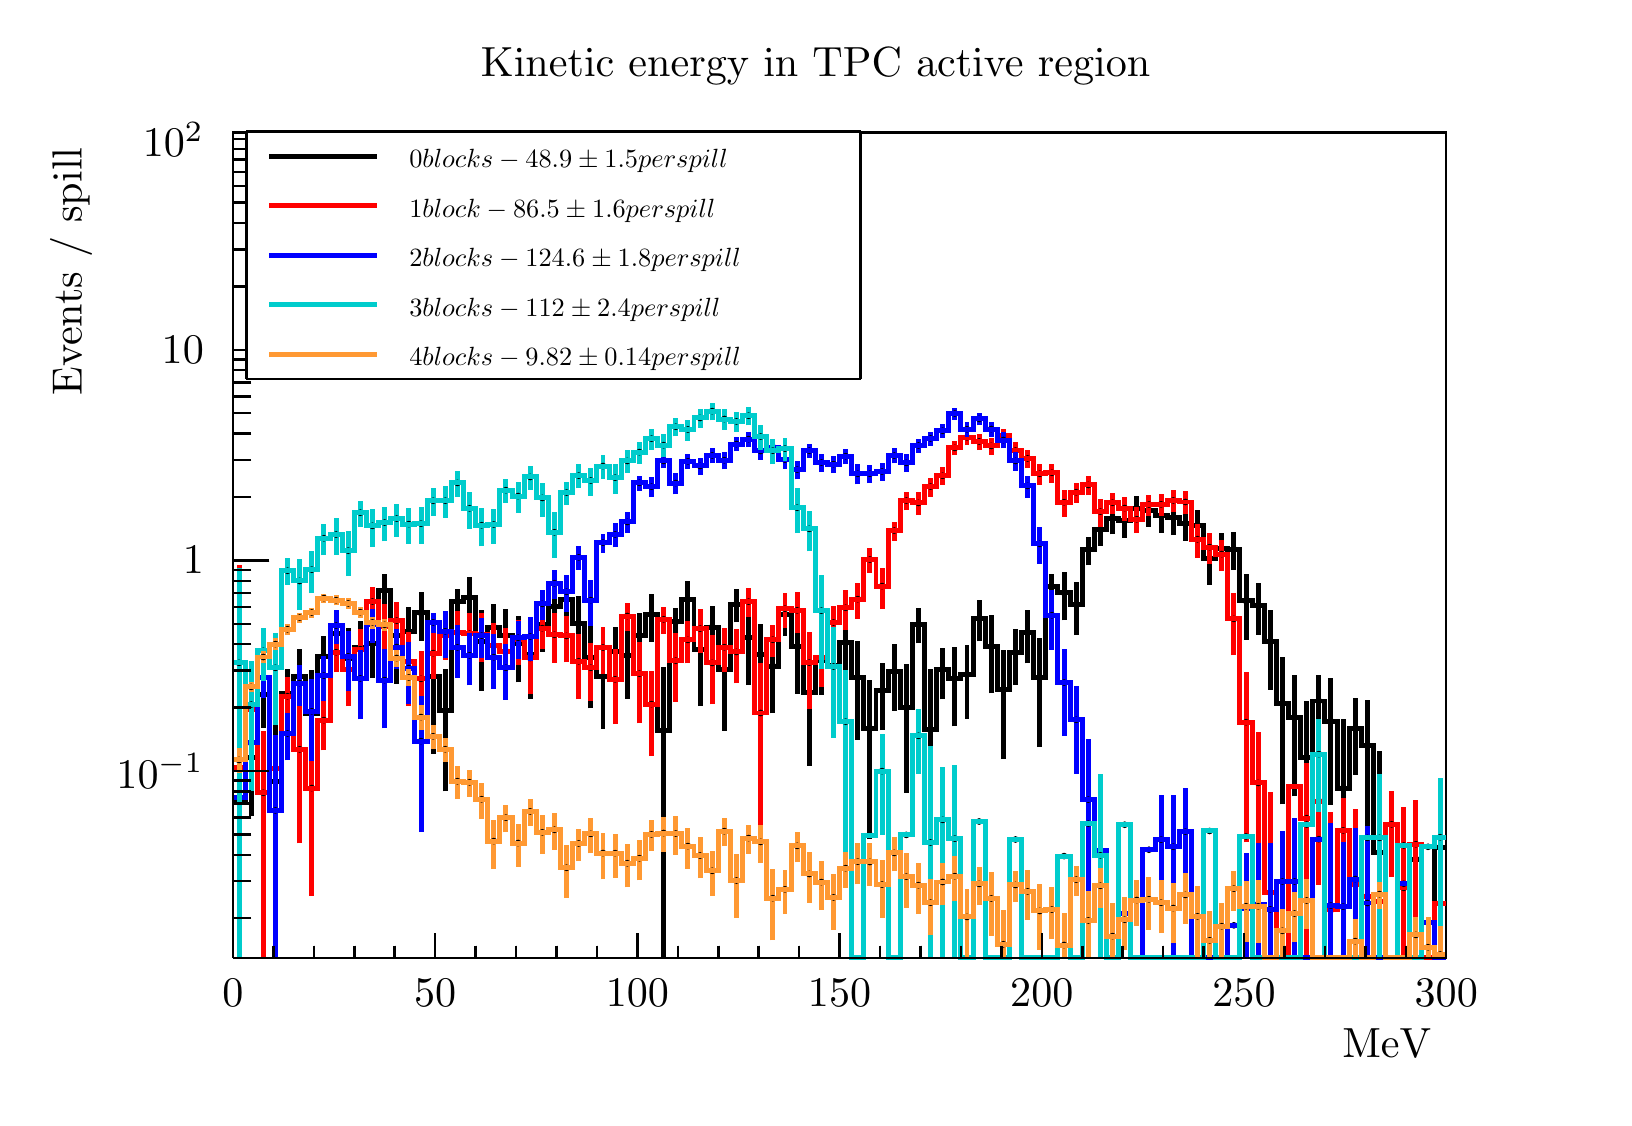
\begin{tikzpicture}
\pgfdeclareplotmark{cross} {
\pgfpathmoveto{\pgfpoint{-0.3\pgfplotmarksize}{\pgfplotmarksize}}
\pgfpathlineto{\pgfpoint{+0.3\pgfplotmarksize}{\pgfplotmarksize}}
\pgfpathlineto{\pgfpoint{+0.3\pgfplotmarksize}{0.3\pgfplotmarksize}}
\pgfpathlineto{\pgfpoint{+1\pgfplotmarksize}{0.3\pgfplotmarksize}}
\pgfpathlineto{\pgfpoint{+1\pgfplotmarksize}{-0.3\pgfplotmarksize}}
\pgfpathlineto{\pgfpoint{+0.3\pgfplotmarksize}{-0.3\pgfplotmarksize}}
\pgfpathlineto{\pgfpoint{+0.3\pgfplotmarksize}{-1.\pgfplotmarksize}}
\pgfpathlineto{\pgfpoint{-0.3\pgfplotmarksize}{-1.\pgfplotmarksize}}
\pgfpathlineto{\pgfpoint{-0.3\pgfplotmarksize}{-0.3\pgfplotmarksize}}
\pgfpathlineto{\pgfpoint{-1.\pgfplotmarksize}{-0.3\pgfplotmarksize}}
\pgfpathlineto{\pgfpoint{-1.\pgfplotmarksize}{0.3\pgfplotmarksize}}
\pgfpathlineto{\pgfpoint{-0.3\pgfplotmarksize}{0.3\pgfplotmarksize}}
\pgfpathclose
\pgfusepathqstroke
}
\pgfdeclareplotmark{cross*} {
\pgfpathmoveto{\pgfpoint{-0.3\pgfplotmarksize}{\pgfplotmarksize}}
\pgfpathlineto{\pgfpoint{+0.3\pgfplotmarksize}{\pgfplotmarksize}}
\pgfpathlineto{\pgfpoint{+0.3\pgfplotmarksize}{0.3\pgfplotmarksize}}
\pgfpathlineto{\pgfpoint{+1\pgfplotmarksize}{0.3\pgfplotmarksize}}
\pgfpathlineto{\pgfpoint{+1\pgfplotmarksize}{-0.3\pgfplotmarksize}}
\pgfpathlineto{\pgfpoint{+0.3\pgfplotmarksize}{-0.3\pgfplotmarksize}}
\pgfpathlineto{\pgfpoint{+0.3\pgfplotmarksize}{-1.\pgfplotmarksize}}
\pgfpathlineto{\pgfpoint{-0.3\pgfplotmarksize}{-1.\pgfplotmarksize}}
\pgfpathlineto{\pgfpoint{-0.3\pgfplotmarksize}{-0.3\pgfplotmarksize}}
\pgfpathlineto{\pgfpoint{-1.\pgfplotmarksize}{-0.3\pgfplotmarksize}}
\pgfpathlineto{\pgfpoint{-1.\pgfplotmarksize}{0.3\pgfplotmarksize}}
\pgfpathlineto{\pgfpoint{-0.3\pgfplotmarksize}{0.3\pgfplotmarksize}}
\pgfpathclose
\pgfusepathqfillstroke
}
\pgfdeclareplotmark{newstar} {
\pgfpathmoveto{\pgfqpoint{0pt}{\pgfplotmarksize}}
\pgfpathlineto{\pgfqpointpolar{44}{0.5\pgfplotmarksize}}
\pgfpathlineto{\pgfqpointpolar{18}{\pgfplotmarksize}}
\pgfpathlineto{\pgfqpointpolar{-20}{0.5\pgfplotmarksize}}
\pgfpathlineto{\pgfqpointpolar{-54}{\pgfplotmarksize}}
\pgfpathlineto{\pgfqpointpolar{-90}{0.5\pgfplotmarksize}}
\pgfpathlineto{\pgfqpointpolar{234}{\pgfplotmarksize}}
\pgfpathlineto{\pgfqpointpolar{198}{0.5\pgfplotmarksize}}
\pgfpathlineto{\pgfqpointpolar{162}{\pgfplotmarksize}}
\pgfpathlineto{\pgfqpointpolar{134}{0.5\pgfplotmarksize}}
\pgfpathclose
\pgfusepathqstroke
}
\pgfdeclareplotmark{newstar*} {
\pgfpathmoveto{\pgfqpoint{0pt}{\pgfplotmarksize}}
\pgfpathlineto{\pgfqpointpolar{44}{0.5\pgfplotmarksize}}
\pgfpathlineto{\pgfqpointpolar{18}{\pgfplotmarksize}}
\pgfpathlineto{\pgfqpointpolar{-20}{0.5\pgfplotmarksize}}
\pgfpathlineto{\pgfqpointpolar{-54}{\pgfplotmarksize}}
\pgfpathlineto{\pgfqpointpolar{-90}{0.5\pgfplotmarksize}}
\pgfpathlineto{\pgfqpointpolar{234}{\pgfplotmarksize}}
\pgfpathlineto{\pgfqpointpolar{198}{0.5\pgfplotmarksize}}
\pgfpathlineto{\pgfqpointpolar{162}{\pgfplotmarksize}}
\pgfpathlineto{\pgfqpointpolar{134}{0.5\pgfplotmarksize}}
\pgfpathclose
\pgfusepathqfillstroke
}
\definecolor{c}{rgb}{1,1,1};
\draw [color=c, fill=c] (0,0) rectangle (20,13.5714);
\draw [color=c, fill=c] (2.6,1.76429) rectangle (18.0086,12.246);
\definecolor{c}{rgb}{0,0,0};
\draw [c,line width=0.9] (2.6,1.76429) -- (2.6,12.246) -- (18.0086,12.246) -- (18.0086,1.76429) -- (2.6,1.76429);
\definecolor{c}{rgb}{1,1,1};
\draw [color=c, fill=c] (2.6,1.76429) rectangle (18.0086,12.246);
\definecolor{c}{rgb}{0,0,0};
\draw [c,line width=0.9] (2.6,1.76429) -- (2.6,12.246) -- (18.0086,12.246) -- (18.0086,1.76429) -- (2.6,1.76429);
\definecolor{c}{rgb}{0,0,0.6};
\draw [c,line width=0.9] (2.6,1.76429) -- (2.75409,1.76429) -- (2.75409,1.76429) -- (2.90817,1.76429) -- (2.90817,1.76429) -- (3.06226,1.76429) -- (3.06226,1.76429) -- (3.21634,1.76429) -- (3.21634,1.76429) -- (3.37043,1.76429) -- (3.37043,1.76429)
 -- (3.52452,1.76429) -- (3.52452,1.76429) -- (3.6786,1.76429) -- (3.6786,1.76429) -- (3.83269,1.76429) -- (3.83269,1.76429) -- (3.98677,1.76429) -- (3.98677,1.76429) -- (4.14086,1.76429) -- (4.14086,1.76429) -- (4.29495,1.76429) -- (4.29495,1.76429)
 -- (4.44903,1.76429) -- (4.44903,1.76429) -- (4.60312,1.76429) -- (4.60312,1.76429) -- (4.7572,1.76429) -- (4.7572,1.76429) -- (4.91129,1.76429) -- (4.91129,1.76429) -- (5.06538,1.76429) -- (5.06538,1.76429) -- (5.21946,1.76429) -- (5.21946,1.76429)
 -- (5.37355,1.76429) -- (5.37355,1.76429) -- (5.52763,1.76429) -- (5.52763,1.76429) -- (5.68172,1.76429) -- (5.68172,1.76429) -- (5.8358,1.76429) -- (5.8358,1.76429) -- (5.98989,1.76429) -- (5.98989,1.76429) -- (6.14398,1.76429) -- (6.14398,1.76429)
 -- (6.29806,1.76429) -- (6.29806,1.76429) -- (6.45215,1.76429) -- (6.45215,1.76429) -- (6.60624,1.76429) -- (6.60624,1.76429) -- (6.76032,1.76429) -- (6.76032,1.76429) -- (6.91441,1.76429) -- (6.91441,1.76429) -- (7.06849,1.76429) --
 (7.06849,1.76429) -- (7.22258,1.76429) -- (7.22258,1.76429) -- (7.37666,1.76429) -- (7.37666,1.76429) -- (7.53075,1.76429) -- (7.53075,1.76429) -- (7.68484,1.76429) -- (7.68484,1.76429) -- (7.83892,1.76429) -- (7.83892,1.76429) -- (7.99301,1.76429)
 -- (7.99301,1.76429) -- (8.14709,1.76429) -- (8.14709,1.76429) -- (8.30118,1.76429) -- (8.30118,1.76429) -- (8.45527,1.76429) -- (8.45527,1.76429) -- (8.60935,1.76429) -- (8.60935,1.76429) -- (8.76344,1.76429) -- (8.76344,1.76429) --
 (8.91752,1.76429) -- (8.91752,1.76429) -- (9.07161,1.76429) -- (9.07161,1.76429) -- (9.2257,1.76429) -- (9.2257,1.76429) -- (9.37978,1.76429) -- (9.37978,1.76429) -- (9.53387,1.76429) -- (9.53387,1.76429) -- (9.68795,1.76429) -- (9.68795,1.76429) --
 (9.84204,1.76429) -- (9.84204,1.76429) -- (9.99613,1.76429) -- (9.99613,1.76429) -- (10.1502,1.76429) -- (10.1502,1.76429) -- (10.3043,1.76429) -- (10.3043,1.76429) -- (10.4584,1.76429) -- (10.4584,1.76429) -- (10.6125,1.76429) -- (10.6125,1.76429)
 -- (10.7666,1.76429) -- (10.7666,1.76429) -- (10.9206,1.76429) -- (10.9206,1.76429) -- (11.0747,1.76429) -- (11.0747,1.76429) -- (11.2288,1.76429) -- (11.2288,1.76429) -- (11.3829,1.76429) -- (11.3829,1.76429) -- (11.537,1.76429) -- (11.537,1.76429)
 -- (11.6911,1.76429) -- (11.6911,1.76429) -- (11.8452,1.76429) -- (11.8452,1.76429) -- (11.9992,1.76429) -- (11.9992,1.76429) -- (12.1533,1.76429) -- (12.1533,1.76429) -- (12.3074,1.76429) -- (12.3074,1.76429) -- (12.4615,1.76429) --
 (12.4615,1.76429) -- (12.6156,1.76429) -- (12.6156,1.76429) -- (12.7697,1.76429) -- (12.7697,1.76429) -- (12.9238,1.76429) -- (12.9238,1.76429) -- (13.0778,1.76429) -- (13.0778,1.76429) -- (13.2319,1.76429) -- (13.2319,1.76429) -- (13.386,1.76429)
 -- (13.386,1.76429) -- (13.5401,1.76429) -- (13.5401,1.76429) -- (13.6942,1.76429) -- (13.6942,1.76429) -- (13.8483,1.76429) -- (13.8483,1.76429) -- (14.0024,1.76429) -- (14.0024,1.76429) -- (14.1564,1.76429) -- (14.1564,1.76429) --
 (14.3105,1.76429) -- (14.3105,1.76429) -- (14.4646,1.76429) -- (14.4646,1.76429) -- (14.6187,1.76429) -- (14.6187,1.76429) -- (14.7728,1.76429) -- (14.7728,1.76429) -- (14.9269,1.76429) -- (14.9269,1.76429) -- (15.081,1.76429) -- (15.081,1.76429) --
 (15.235,1.76429) -- (15.235,1.76429) -- (15.3891,1.76429) -- (15.3891,1.76429) -- (15.5432,1.76429) -- (15.5432,1.76429) -- (15.6973,1.76429) -- (15.6973,1.76429) -- (15.8514,1.76429) -- (15.8514,1.76429) -- (16.0055,1.76429) -- (16.0055,1.76429) --
 (16.1596,1.76429) -- (16.1596,1.76429) -- (16.3137,1.76429) -- (16.3137,1.76429) -- (16.4677,1.76429) -- (16.4677,1.76429) -- (16.6218,1.76429) -- (16.6218,1.76429) -- (16.7759,1.76429) -- (16.7759,1.76429) -- (16.93,1.76429) -- (16.93,1.76429) --
 (17.0841,1.76429) -- (17.0841,1.76429) -- (17.2382,1.76429) -- (17.2382,1.76429) -- (17.3923,1.76429) -- (17.3923,1.76429) -- (17.5463,1.76429) -- (17.5463,1.76429) -- (17.7004,1.76429) -- (17.7004,1.76429) -- (17.8545,1.76429) -- (17.8545,1.76429)
 -- (18.0086,1.76429);
\definecolor{c}{rgb}{0,0,0};
\draw [c,line width=0.9] (2.6,1.76429) -- (18.0086,1.76429);
\draw [c,line width=0.9] (2.6,2.07796) -- (2.6,1.76429);
\draw [c,line width=0.9] (3.11362,1.92112) -- (3.11362,1.76429);
\draw [c,line width=0.9] (3.62724,1.92112) -- (3.62724,1.76429);
\draw [c,line width=0.9] (4.14086,1.92112) -- (4.14086,1.76429);
\draw [c,line width=0.9] (4.65448,1.92112) -- (4.65448,1.76429);
\draw [c,line width=0.9] (5.1681,2.07796) -- (5.1681,1.76429);
\draw [c,line width=0.9] (5.68172,1.92112) -- (5.68172,1.76429);
\draw [c,line width=0.9] (6.19534,1.92112) -- (6.19534,1.76429);
\draw [c,line width=0.9] (6.70896,1.92112) -- (6.70896,1.76429);
\draw [c,line width=0.9] (7.22258,1.92112) -- (7.22258,1.76429);
\draw [c,line width=0.9] (7.7362,2.07796) -- (7.7362,1.76429);
\draw [c,line width=0.9] (8.24982,1.92112) -- (8.24982,1.76429);
\draw [c,line width=0.9] (8.76344,1.92112) -- (8.76344,1.76429);
\draw [c,line width=0.9] (9.27706,1.92112) -- (9.27706,1.76429);
\draw [c,line width=0.9] (9.79068,1.92112) -- (9.79068,1.76429);
\draw [c,line width=0.9] (10.3043,2.07796) -- (10.3043,1.76429);
\draw [c,line width=0.9] (10.8179,1.92112) -- (10.8179,1.76429);
\draw [c,line width=0.9] (11.3315,1.92112) -- (11.3315,1.76429);
\draw [c,line width=0.9] (11.8452,1.92112) -- (11.8452,1.76429);
\draw [c,line width=0.9] (12.3588,1.92112) -- (12.3588,1.76429);
\draw [c,line width=0.9] (12.8724,2.07796) -- (12.8724,1.76429);
\draw [c,line width=0.9] (13.386,1.92112) -- (13.386,1.76429);
\draw [c,line width=0.9] (13.8996,1.92112) -- (13.8996,1.76429);
\draw [c,line width=0.9] (14.4133,1.92112) -- (14.4133,1.76429);
\draw [c,line width=0.9] (14.9269,1.92112) -- (14.9269,1.76429);
\draw [c,line width=0.9] (15.4405,2.07796) -- (15.4405,1.76429);
\draw [c,line width=0.9] (15.9541,1.92112) -- (15.9541,1.76429);
\draw [c,line width=0.9] (16.4677,1.92112) -- (16.4677,1.76429);
\draw [c,line width=0.9] (16.9814,1.92112) -- (16.9814,1.76429);
\draw [c,line width=0.9] (17.495,1.92112) -- (17.495,1.76429);
\draw [c,line width=0.9] (18.0086,2.07796) -- (18.0086,1.76429);
\draw [anchor=base] (2.6,1.15357) node[scale=1.52295, color=c, rotate=0]{0};
\draw [anchor=base] (5.1681,1.15357) node[scale=1.52295, color=c, rotate=0]{50};
\draw [anchor=base] (7.7362,1.15357) node[scale=1.52295, color=c, rotate=0]{100};
\draw [anchor=base] (10.3043,1.15357) node[scale=1.52295, color=c, rotate=0]{150};
\draw [anchor=base] (12.8724,1.15357) node[scale=1.52295, color=c, rotate=0]{200};
\draw [anchor=base] (15.4405,1.15357) node[scale=1.52295, color=c, rotate=0]{250};
\draw [anchor=base] (18.0086,1.15357) node[scale=1.52295, color=c, rotate=0]{300};
\draw [anchor= east] (18.0086,0.678571) node[scale=1.52295, color=c, rotate=0]{ MeV};
\draw [c,line width=0.9] (2.6,1.76429) -- (2.6,12.246);
\draw [c,line width=0.9] (2.8317,2.26869) -- (2.6,2.26869);
\draw [c,line width=0.9] (2.8317,2.73968) -- (2.6,2.73968);
\draw [c,line width=0.9] (2.8317,3.07386) -- (2.6,3.07386);
\draw [c,line width=0.9] (2.8317,3.33307) -- (2.6,3.33307);
\draw [c,line width=0.9] (2.8317,3.54485) -- (2.6,3.54485);
\draw [c,line width=0.9] (2.8317,3.72392) -- (2.6,3.72392);
\draw [c,line width=0.9] (2.8317,3.87903) -- (2.6,3.87903);
\draw [c,line width=0.9] (2.8317,4.01585) -- (2.6,4.01585);
\draw [c,line width=0.9] (3.0634,4.13824) -- (2.6,4.13824);
\draw [anchor= east] (2.42,4.13824) node[scale=1.52295, color=c, rotate=0]{$10^{-1}$};
\draw [c,line width=0.9] (2.8317,4.94341) -- (2.6,4.94341);
\draw [c,line width=0.9] (2.8317,5.41441) -- (2.6,5.41441);
\draw [c,line width=0.9] (2.8317,5.74858) -- (2.6,5.74858);
\draw [c,line width=0.9] (2.8317,6.00779) -- (2.6,6.00779);
\draw [c,line width=0.9] (2.8317,6.21958) -- (2.6,6.21958);
\draw [c,line width=0.9] (2.8317,6.39864) -- (2.6,6.39864);
\draw [c,line width=0.9] (2.8317,6.55375) -- (2.6,6.55375);
\draw [c,line width=0.9] (2.8317,6.69057) -- (2.6,6.69057);
\draw [c,line width=0.9] (3.0634,6.81296) -- (2.6,6.81296);
\draw [anchor= east] (2.42,6.81296) node[scale=1.52295, color=c, rotate=0]{1};
\draw [c,line width=0.9] (2.8317,7.61813) -- (2.6,7.61813);
\draw [c,line width=0.9] (2.8317,8.08913) -- (2.6,8.08913);
\draw [c,line width=0.9] (2.8317,8.4233) -- (2.6,8.4233);
\draw [c,line width=0.9] (2.8317,8.68251) -- (2.6,8.68251);
\draw [c,line width=0.9] (2.8317,8.8943) -- (2.6,8.8943);
\draw [c,line width=0.9] (2.8317,9.07336) -- (2.6,9.07336);
\draw [c,line width=0.9] (2.8317,9.22848) -- (2.6,9.22848);
\draw [c,line width=0.9] (2.8317,9.3653) -- (2.6,9.3653);
\draw [c,line width=0.9] (3.0634,9.48768) -- (2.6,9.48768);
\draw [anchor= east] (2.42,9.48768) node[scale=1.52295, color=c, rotate=0]{10};
\draw [c,line width=0.9] (2.8317,10.2929) -- (2.6,10.2929);
\draw [c,line width=0.9] (2.8317,10.7639) -- (2.6,10.7639);
\draw [c,line width=0.9] (2.8317,11.098) -- (2.6,11.098);
\draw [c,line width=0.9] (2.8317,11.3572) -- (2.6,11.3572);
\draw [c,line width=0.9] (2.8317,11.569) -- (2.6,11.569);
\draw [c,line width=0.9] (2.8317,11.7481) -- (2.6,11.7481);
\draw [c,line width=0.9] (2.8317,11.9032) -- (2.6,11.9032);
\draw [c,line width=0.9] (2.8317,12.04) -- (2.6,12.04);
\draw [c,line width=0.9] (3.0634,12.1624) -- (2.6,12.1624);
\draw [anchor= east] (2.42,12.1624) node[scale=1.52295, color=c, rotate=0]{$10^{2}$};
\draw [anchor= east] (0.542857,12.246) node[scale=1.52295, color=c, rotate=90]{ Events / spill};
\draw [c,line width=1.8] (2.67704,1.76429) -- (2.67704,3.77788);
\draw [c,line width=1.8] (2.67704,3.77788) -- (2.67704,6.72463);
\foreach \P in {(2.67704,3.77788)}{\draw[mark options={color=c,fill=c},mark size=2.402402pt,mark=*,mark size=1pt] plot coordinates {\P};}
\draw [c,line width=1.8] (2.83113,3.5658) -- (2.83113,4.30569);
\draw [c,line width=1.8] (2.83113,4.30569) -- (2.83113,4.75409);
\foreach \P in {(2.83113,4.30569)}{\draw[mark options={color=c,fill=c},mark size=2.402402pt,mark=*,mark size=1pt] plot coordinates {\P};}
\draw [c,line width=1.8] (2.98521,4.68707) -- (2.98521,5.1098);
\draw [c,line width=1.8] (2.98521,5.1098) -- (2.98521,5.41907);
\foreach \P in {(2.98521,5.1098)}{\draw[mark options={color=c,fill=c},mark size=2.402402pt,mark=*,mark size=1pt] plot coordinates {\P};}
\draw [c,line width=1.8] (3.1393,1.76429) -- (3.1393,4.00405);
\draw [c,line width=1.8] (3.1393,4.00405) -- (3.1393,4.87417);
\foreach \P in {(3.1393,4.00405)}{\draw[mark options={color=c,fill=c},mark size=2.402402pt,mark=*,mark size=1pt] plot coordinates {\P};}
\draw [c,line width=1.8] (3.29339,4.72446) -- (3.29339,5.12855);
\draw [c,line width=1.8] (3.29339,5.12855) -- (3.29339,5.42776);
\foreach \P in {(3.29339,5.12855)}{\draw[mark options={color=c,fill=c},mark size=2.402402pt,mark=*,mark size=1pt] plot coordinates {\P};}
\draw [c,line width=1.8] (3.44747,4.81085) -- (3.44747,5.33313);
\draw [c,line width=1.8] (3.44747,5.33313) -- (3.44747,5.69213);
\foreach \P in {(3.44747,5.33313)}{\draw[mark options={color=c,fill=c},mark size=2.402402pt,mark=*,mark size=1pt] plot coordinates {\P};}
\draw [c,line width=1.8] (3.60156,3.78971) -- (3.60156,4.86945);
\draw [c,line width=1.8] (3.60156,4.86945) -- (3.60156,5.41922);
\foreach \P in {(3.60156,4.86945)}{\draw[mark options={color=c,fill=c},mark size=2.402402pt,mark=*,mark size=1pt] plot coordinates {\P};}
\draw [c,line width=1.8] (3.75564,5.2544) -- (3.75564,5.59407);
\draw [c,line width=1.8] (3.75564,5.59407) -- (3.75564,5.85657);
\foreach \P in {(3.75564,5.59407)}{\draw[mark options={color=c,fill=c},mark size=2.402402pt,mark=*,mark size=1pt] plot coordinates {\P};}
\draw [c,line width=1.8] (3.90973,5.50649) -- (3.90973,5.88154);
\draw [c,line width=1.8] (3.90973,5.88154) -- (3.90973,6.16459);
\foreach \P in {(3.90973,5.88154)}{\draw[mark options={color=c,fill=c},mark size=2.402402pt,mark=*,mark size=1pt] plot coordinates {\P};}
\draw [c,line width=1.8] (4.06382,4.98513) -- (4.06382,5.57167);
\draw [c,line width=1.8] (4.06382,5.57167) -- (4.06382,5.95957);
\foreach \P in {(4.06382,5.57167)}{\draw[mark options={color=c,fill=c},mark size=2.402402pt,mark=*,mark size=1pt] plot coordinates {\P};}
\draw [c,line width=1.8] (4.2179,5.21896) -- (4.2179,5.70174);
\draw [c,line width=1.8] (4.2179,5.70174) -- (4.2179,6.04177);
\foreach \P in {(4.2179,5.70174)}{\draw[mark options={color=c,fill=c},mark size=2.402402pt,mark=*,mark size=1pt] plot coordinates {\P};}
\draw [c,line width=1.8] (4.37199,5.31802) -- (4.37199,5.76129);
\draw [c,line width=1.8] (4.37199,5.76129) -- (4.37199,6.08134);
\foreach \P in {(4.37199,5.76129)}{\draw[mark options={color=c,fill=c},mark size=2.402402pt,mark=*,mark size=1pt] plot coordinates {\P};}
\draw [c,line width=1.8] (4.52607,6.19429) -- (4.52607,6.43603);
\draw [c,line width=1.8] (4.52607,6.43603) -- (4.52607,6.63602);
\foreach \P in {(4.52607,6.43603)}{\draw[mark options={color=c,fill=c},mark size=2.402402pt,mark=*,mark size=1pt] plot coordinates {\P};}
\draw [c,line width=1.8] (4.68016,5.24509) -- (4.68016,5.85988);
\draw [c,line width=1.8] (4.68016,5.85988) -- (4.68016,6.25979);
\foreach \P in {(4.68016,5.85988)}{\draw[mark options={color=c,fill=c},mark size=2.402402pt,mark=*,mark size=1pt] plot coordinates {\P};}
\draw [c,line width=1.8] (4.83425,5.4672) -- (4.83425,5.90683);
\draw [c,line width=1.8] (4.83425,5.90683) -- (4.83425,6.225);
\foreach \P in {(4.83425,5.90683)}{\draw[mark options={color=c,fill=c},mark size=2.402402pt,mark=*,mark size=1pt] plot coordinates {\P};}
\draw [c,line width=1.8] (4.98833,5.78993) -- (4.98833,6.14503);
\draw [c,line width=1.8] (4.98833,6.14503) -- (4.98833,6.41661);
\foreach \P in {(4.98833,6.14503)}{\draw[mark options={color=c,fill=c},mark size=2.402402pt,mark=*,mark size=1pt] plot coordinates {\P};}
\draw [c,line width=1.8] (5.14242,4.35521) -- (5.14242,5.338);
\draw [c,line width=1.8] (5.14242,5.338) -- (5.14242,5.86264);
\foreach \P in {(5.14242,5.338)}{\draw[mark options={color=c,fill=c},mark size=2.402402pt,mark=*,mark size=1pt] plot coordinates {\P};}
\draw [c,line width=1.8] (5.2965,3.87979) -- (5.2965,4.90083);
\draw [c,line width=1.8] (5.2965,4.90083) -- (5.2965,5.4357);
\foreach \P in {(5.2965,4.90083)}{\draw[mark options={color=c,fill=c},mark size=2.402402pt,mark=*,mark size=1pt] plot coordinates {\P};}
\draw [c,line width=1.8] (5.45059,6.11314) -- (5.45059,6.29195);
\draw [c,line width=1.8] (5.45059,6.29195) -- (5.45059,6.44687);
\foreach \P in {(5.45059,6.29195)}{\draw[mark options={color=c,fill=c},mark size=2.402402pt,mark=*,mark size=1pt] plot coordinates {\P};}
\draw [c,line width=1.8] (5.60468,5.98904) -- (5.60468,6.33729);
\draw [c,line width=1.8] (5.60468,6.33729) -- (5.60468,6.60486);
\foreach \P in {(5.60468,6.33729)}{\draw[mark options={color=c,fill=c},mark size=2.402402pt,mark=*,mark size=1pt] plot coordinates {\P};}
\draw [c,line width=1.8] (5.75876,5.15619) -- (5.75876,5.78044);
\draw [c,line width=1.8] (5.75876,5.78044) -- (5.75876,6.18427);
\foreach \P in {(5.75876,5.78044)}{\draw[mark options={color=c,fill=c},mark size=2.402402pt,mark=*,mark size=1pt] plot coordinates {\P};}
\draw [c,line width=1.8] (5.91285,5.56776) -- (5.91285,5.96517);
\draw [c,line width=1.8] (5.91285,5.96517) -- (5.91285,6.26073);
\foreach \P in {(5.91285,5.96517)}{\draw[mark options={color=c,fill=c},mark size=2.402402pt,mark=*,mark size=1pt] plot coordinates {\P};}
\draw [c,line width=1.8] (6.06693,5.38116) -- (6.06693,5.86042);
\draw [c,line width=1.8] (6.06693,5.86042) -- (6.06693,6.19871);
\foreach \P in {(6.06693,5.86042)}{\draw[mark options={color=c,fill=c},mark size=2.402402pt,mark=*,mark size=1pt] plot coordinates {\P};}
\draw [c,line width=1.8] (6.22102,5.26273) -- (6.22102,5.76223);
\draw [c,line width=1.8] (6.22102,5.76223) -- (6.22102,6.11039);
\foreach \P in {(6.22102,5.76223)}{\draw[mark options={color=c,fill=c},mark size=2.402402pt,mark=*,mark size=1pt] plot coordinates {\P};}
\draw [c,line width=1.8] (6.37511,5.05382) -- (6.37511,5.61642);
\draw [c,line width=1.8] (6.37511,5.61642) -- (6.37511,5.99382);
\foreach \P in {(6.37511,5.61642)}{\draw[mark options={color=c,fill=c},mark size=2.402402pt,mark=*,mark size=1pt] plot coordinates {\P};}
\draw [c,line width=1.8] (6.52919,5.65496) -- (6.52919,5.99633);
\draw [c,line width=1.8] (6.52919,5.99633) -- (6.52919,6.25982);
\foreach \P in {(6.52919,5.99633)}{\draw[mark options={color=c,fill=c},mark size=2.402402pt,mark=*,mark size=1pt] plot coordinates {\P};}
\draw [c,line width=1.8] (6.68328,5.91103) -- (6.68328,6.2293);
\draw [c,line width=1.8] (6.68328,6.2293) -- (6.68328,6.47886);
\foreach \P in {(6.68328,6.2293)}{\draw[mark options={color=c,fill=c},mark size=2.402402pt,mark=*,mark size=1pt] plot coordinates {\P};}
\draw [c,line width=1.8] (6.83736,5.96848) -- (6.83736,6.31384);
\draw [c,line width=1.8] (6.83736,6.31384) -- (6.83736,6.5797);
\foreach \P in {(6.83736,6.31384)}{\draw[mark options={color=c,fill=c},mark size=2.402402pt,mark=*,mark size=1pt] plot coordinates {\P};}
\draw [c,line width=1.8] (6.99145,5.52099) -- (6.99145,6.01339);
\draw [c,line width=1.8] (6.99145,6.01339) -- (6.99145,6.35813);
\foreach \P in {(6.99145,6.01339)}{\draw[mark options={color=c,fill=c},mark size=2.402402pt,mark=*,mark size=1pt] plot coordinates {\P};}
\draw [c,line width=1.8] (7.14554,4.93495) -- (7.14554,5.58107);
\draw [c,line width=1.8] (7.14554,5.58107) -- (7.14554,5.99382);
\foreach \P in {(7.14554,5.58107)}{\draw[mark options={color=c,fill=c},mark size=2.402402pt,mark=*,mark size=1pt] plot coordinates {\P};}
\draw [c,line width=1.8] (7.29962,4.67176) -- (7.29962,5.33589);
\draw [c,line width=1.8] (7.29962,5.33589) -- (7.29962,5.7558);
\foreach \P in {(7.29962,5.33589)}{\draw[mark options={color=c,fill=c},mark size=2.402402pt,mark=*,mark size=1pt] plot coordinates {\P};}
\draw [c,line width=1.8] (7.45371,5.2341) -- (7.45371,5.65629);
\draw [c,line width=1.8] (7.45371,5.65629) -- (7.45371,5.96527);
\foreach \P in {(7.45371,5.65629)}{\draw[mark options={color=c,fill=c},mark size=2.402402pt,mark=*,mark size=1pt] plot coordinates {\P};}
\draw [c,line width=1.8] (7.60779,5.05511) -- (7.60779,5.60054);
\draw [c,line width=1.8] (7.60779,5.60054) -- (7.60779,5.97022);
\foreach \P in {(7.60779,5.60054)}{\draw[mark options={color=c,fill=c},mark size=2.402402pt,mark=*,mark size=1pt] plot coordinates {\P};}
\draw [c,line width=1.8] (7.76188,5.46398) -- (7.76188,5.85452);
\draw [c,line width=1.8] (7.76188,5.85452) -- (7.76188,6.14627);
\foreach \P in {(7.76188,5.85452)}{\draw[mark options={color=c,fill=c},mark size=2.402402pt,mark=*,mark size=1pt] plot coordinates {\P};}
\draw [c,line width=1.8] (7.91597,5.77694) -- (7.91597,6.11972);
\draw [c,line width=1.8] (7.91597,6.11972) -- (7.91597,6.38406);
\foreach \P in {(7.91597,6.11972)}{\draw[mark options={color=c,fill=c},mark size=2.402402pt,mark=*,mark size=1pt] plot coordinates {\P};}
\draw [c,line width=1.8] (8.07005,1.76429) -- (8.07005,4.64807);
\draw [c,line width=1.8] (8.07005,4.64807) -- (8.07005,5.45715);
\foreach \P in {(8.07005,4.64807)}{\draw[mark options={color=c,fill=c},mark size=2.402402pt,mark=*,mark size=1pt] plot coordinates {\P};}
\draw [c,line width=1.8] (8.22414,5.8299) -- (8.22414,6.03235);
\draw [c,line width=1.8] (8.22414,6.03235) -- (8.22414,6.2047);
\foreach \P in {(8.22414,6.03235)}{\draw[mark options={color=c,fill=c},mark size=2.402402pt,mark=*,mark size=1pt] plot coordinates {\P};}
\draw [c,line width=1.8] (8.37822,6.01039) -- (8.37822,6.31539);
\draw [c,line width=1.8] (8.37822,6.31539) -- (8.37822,6.55674);
\foreach \P in {(8.37822,6.31539)}{\draw[mark options={color=c,fill=c},mark size=2.402402pt,mark=*,mark size=1pt] plot coordinates {\P};}
\draw [c,line width=1.8] (8.53231,4.96303) -- (8.53231,5.68001);
\draw [c,line width=1.8] (8.53231,5.68001) -- (8.53231,6.12006);
\foreach \P in {(8.53231,5.68001)}{\draw[mark options={color=c,fill=c},mark size=2.402402pt,mark=*,mark size=1pt] plot coordinates {\P};}
\draw [c,line width=1.8] (8.6864,5.61271) -- (8.6864,5.96463);
\draw [c,line width=1.8] (8.6864,5.96463) -- (8.6864,6.23436);
\foreach \P in {(8.6864,5.96463)}{\draw[mark options={color=c,fill=c},mark size=2.402402pt,mark=*,mark size=1pt] plot coordinates {\P};}
\draw [c,line width=1.8] (8.84048,4.65006) -- (8.84048,5.42613);
\draw [c,line width=1.8] (8.84048,5.42613) -- (8.84048,5.88726);
\foreach \P in {(8.84048,5.42613)}{\draw[mark options={color=c,fill=c},mark size=2.402402pt,mark=*,mark size=1pt] plot coordinates {\P};}
\draw [c,line width=1.8] (8.99457,6.02467) -- (8.99457,6.25817);
\draw [c,line width=1.8] (8.99457,6.25817) -- (8.99457,6.45249);
\foreach \P in {(8.99457,6.25817)}{\draw[mark options={color=c,fill=c},mark size=2.402402pt,mark=*,mark size=1pt] plot coordinates {\P};}
\draw [c,line width=1.8] (9.14865,5.22873) -- (9.14865,5.8336);
\draw [c,line width=1.8] (9.14865,5.8336) -- (9.14865,6.22934);
\foreach \P in {(9.14865,5.8336)}{\draw[mark options={color=c,fill=c},mark size=2.402402pt,mark=*,mark size=1pt] plot coordinates {\P};}
\draw [c,line width=1.8] (9.30274,5.0546) -- (9.30274,5.62089);
\draw [c,line width=1.8] (9.30274,5.62089) -- (9.30274,5.99994);
\foreach \P in {(9.30274,5.62089)}{\draw[mark options={color=c,fill=c},mark size=2.402402pt,mark=*,mark size=1pt] plot coordinates {\P};}
\draw [c,line width=1.8] (9.45683,4.87098) -- (9.45683,5.47114);
\draw [c,line width=1.8] (9.45683,5.47114) -- (9.45683,5.86489);
\foreach \P in {(9.45683,5.47114)}{\draw[mark options={color=c,fill=c},mark size=2.402402pt,mark=*,mark size=1pt] plot coordinates {\P};}
\draw [c,line width=1.8] (9.61091,5.85157) -- (9.61091,6.12942);
\draw [c,line width=1.8] (9.61091,6.12942) -- (9.61091,6.35347);
\foreach \P in {(9.61091,6.12942)}{\draw[mark options={color=c,fill=c},mark size=2.402402pt,mark=*,mark size=1pt] plot coordinates {\P};}
\draw [c,line width=1.8] (9.765,5.11705) -- (9.765,5.71956);
\draw [c,line width=1.8] (9.765,5.71956) -- (9.765,6.1143);
\foreach \P in {(9.765,5.71956)}{\draw[mark options={color=c,fill=c},mark size=2.402402pt,mark=*,mark size=1pt] plot coordinates {\P};}
\draw [c,line width=1.8] (9.91908,4.20269) -- (9.91908,5.13908);
\draw [c,line width=1.8] (9.91908,5.13908) -- (9.91908,5.65072);
\foreach \P in {(9.91908,5.13908)}{\draw[mark options={color=c,fill=c},mark size=2.402402pt,mark=*,mark size=1pt] plot coordinates {\P};}
\draw [c,line width=1.8] (10.0732,5.10691) -- (10.0732,5.53685);
\draw [c,line width=1.8] (10.0732,5.53685) -- (10.0732,5.84995);
\foreach \P in {(10.0732,5.53685)}{\draw[mark options={color=c,fill=c},mark size=2.402402pt,mark=*,mark size=1pt] plot coordinates {\P};}
\draw [c,line width=1.8] (10.2273,4.88648) -- (10.2273,5.48144);
\draw [c,line width=1.8] (10.2273,5.48144) -- (10.2273,5.87297);
\foreach \P in {(10.2273,5.48144)}{\draw[mark options={color=c,fill=c},mark size=2.402402pt,mark=*,mark size=1pt] plot coordinates {\P};}
\draw [c,line width=1.8] (10.3813,5.36186) -- (10.3813,5.7643);
\draw [c,line width=1.8] (10.3813,5.7643) -- (10.3813,6.06261);
\foreach \P in {(10.3813,5.7643)}{\draw[mark options={color=c,fill=c},mark size=2.402402pt,mark=*,mark size=1pt] plot coordinates {\P};}
\draw [c,line width=1.8] (10.5354,4.53355) -- (10.5354,5.32592);
\draw [c,line width=1.8] (10.5354,5.32592) -- (10.5354,5.79262);
\foreach \P in {(10.5354,5.32592)}{\draw[mark options={color=c,fill=c},mark size=2.402402pt,mark=*,mark size=1pt] plot coordinates {\P};}
\draw [c,line width=1.8] (10.6895,3.27066) -- (10.6895,4.67924);
\draw [c,line width=1.8] (10.6895,4.67924) -- (10.6895,5.29739);
\foreach \P in {(10.6895,4.67924)}{\draw[mark options={color=c,fill=c},mark size=2.402402pt,mark=*,mark size=1pt] plot coordinates {\P};}
\draw [c,line width=1.8] (10.8436,4.65855) -- (10.8436,5.16052);
\draw [c,line width=1.8] (10.8436,5.16052) -- (10.8436,5.50989);
\foreach \P in {(10.8436,5.16052)}{\draw[mark options={color=c,fill=c},mark size=2.402402pt,mark=*,mark size=1pt] plot coordinates {\P};}
\draw [c,line width=1.8] (10.9977,4.90254) -- (10.9977,5.40524);
\draw [c,line width=1.8] (10.9977,5.40524) -- (10.9977,5.75495);
\foreach \P in {(10.9977,5.40524)}{\draw[mark options={color=c,fill=c},mark size=2.402402pt,mark=*,mark size=1pt] plot coordinates {\P};}
\draw [c,line width=1.8] (11.1518,3.86489) -- (11.1518,4.94261);
\draw [c,line width=1.8] (11.1518,4.94261) -- (11.1518,5.49188);
\foreach \P in {(11.1518,4.94261)}{\draw[mark options={color=c,fill=c},mark size=2.402402pt,mark=*,mark size=1pt] plot coordinates {\P};}
\draw [c,line width=1.8] (11.3059,5.75797) -- (11.3059,6.00379);
\draw [c,line width=1.8] (11.3059,6.00379) -- (11.3059,6.20656);
\foreach \P in {(11.3059,6.00379)}{\draw[mark options={color=c,fill=c},mark size=2.402402pt,mark=*,mark size=1pt] plot coordinates {\P};}
\draw [c,line width=1.8] (11.4599,1.76429) -- (11.4599,4.66394);
\draw [c,line width=1.8] (11.4599,4.66394) -- (11.4599,5.43043);
\foreach \P in {(11.4599,4.66394)}{\draw[mark options={color=c,fill=c},mark size=2.402402pt,mark=*,mark size=1pt] plot coordinates {\P};}
\draw [c,line width=1.8] (11.614,5.04677) -- (11.614,5.42129);
\draw [c,line width=1.8] (11.614,5.42129) -- (11.614,5.70404);
\foreach \P in {(11.614,5.42129)}{\draw[mark options={color=c,fill=c},mark size=2.402402pt,mark=*,mark size=1pt] plot coordinates {\P};}
\draw [c,line width=1.8] (11.7681,4.70379) -- (11.7681,5.31392);
\draw [c,line width=1.8] (11.7681,5.31392) -- (11.7681,5.71187);
\foreach \P in {(11.7681,5.31392)}{\draw[mark options={color=c,fill=c},mark size=2.402402pt,mark=*,mark size=1pt] plot coordinates {\P};}
\draw [c,line width=1.8] (11.9222,4.8006) -- (11.9222,5.36395);
\draw [c,line width=1.8] (11.9222,5.36395) -- (11.9222,5.74169);
\foreach \P in {(11.9222,5.36395)}{\draw[mark options={color=c,fill=c},mark size=2.402402pt,mark=*,mark size=1pt] plot coordinates {\P};}
\draw [c,line width=1.8] (12.0763,5.78399) -- (12.0763,6.07357);
\draw [c,line width=1.8] (12.0763,6.07357) -- (12.0763,6.30517);
\foreach \P in {(12.0763,6.07357)}{\draw[mark options={color=c,fill=c},mark size=2.402402pt,mark=*,mark size=1pt] plot coordinates {\P};}
\draw [c,line width=1.8] (12.2304,5.12273) -- (12.2304,5.7204);
\draw [c,line width=1.8] (12.2304,5.7204) -- (12.2304,6.11308);
\foreach \P in {(12.2304,5.7204)}{\draw[mark options={color=c,fill=c},mark size=2.402402pt,mark=*,mark size=1pt] plot coordinates {\P};}
\draw [c,line width=1.8] (12.3845,4.28801) -- (12.3845,5.17713);
\draw [c,line width=1.8] (12.3845,5.17713) -- (12.3845,5.67481);
\foreach \P in {(12.3845,5.17713)}{\draw[mark options={color=c,fill=c},mark size=2.402402pt,mark=*,mark size=1pt] plot coordinates {\P};}
\draw [c,line width=1.8] (12.5385,5.22968) -- (12.5385,5.63771);
\draw [c,line width=1.8] (12.5385,5.63771) -- (12.5385,5.93908);
\foreach \P in {(12.5385,5.63771)}{\draw[mark options={color=c,fill=c},mark size=2.402402pt,mark=*,mark size=1pt] plot coordinates {\P};}
\draw [c,line width=1.8] (12.6926,5.5047) -- (12.6926,5.89348);
\draw [c,line width=1.8] (12.6926,5.89348) -- (12.6926,6.18426);
\foreach \P in {(12.6926,5.89348)}{\draw[mark options={color=c,fill=c},mark size=2.402402pt,mark=*,mark size=1pt] plot coordinates {\P};}
\draw [c,line width=1.8] (12.8467,4.44291) -- (12.8467,5.32568);
\draw [c,line width=1.8] (12.8467,5.32568) -- (12.8467,5.82143);
\foreach \P in {(12.8467,5.32568)}{\draw[mark options={color=c,fill=c},mark size=2.402402pt,mark=*,mark size=1pt] plot coordinates {\P};}
\draw [c,line width=1.8] (13.0008,6.29352) -- (13.0008,6.47959);
\draw [c,line width=1.8] (13.0008,6.47959) -- (13.0008,6.63992);
\foreach \P in {(13.0008,6.47959)}{\draw[mark options={color=c,fill=c},mark size=2.402402pt,mark=*,mark size=1pt] plot coordinates {\P};}
\draw [c,line width=1.8] (13.1549,6.05013) -- (13.1549,6.4015);
\draw [c,line width=1.8] (13.1549,6.4015) -- (13.1549,6.6709);
\foreach \P in {(13.1549,6.4015)}{\draw[mark options={color=c,fill=c},mark size=2.402402pt,mark=*,mark size=1pt] plot coordinates {\P};}
\draw [c,line width=1.8] (13.309,5.86485) -- (13.309,6.25257);
\draw [c,line width=1.8] (13.309,6.25257) -- (13.309,6.54276);
\foreach \P in {(13.309,6.25257)}{\draw[mark options={color=c,fill=c},mark size=2.402402pt,mark=*,mark size=1pt] plot coordinates {\P};}
\draw [c,line width=1.8] (13.4631,6.75067) -- (13.4631,6.94528);
\draw [c,line width=1.8] (13.4631,6.94528) -- (13.4631,7.11192);
\foreach \P in {(13.4631,6.94528)}{\draw[mark options={color=c,fill=c},mark size=2.402402pt,mark=*,mark size=1pt] plot coordinates {\P};}
\draw [c,line width=1.8] (13.6171,6.99949) -- (13.6171,7.20433);
\draw [c,line width=1.8] (13.6171,7.20433) -- (13.6171,7.37841);
\foreach \P in {(13.6171,7.20433)}{\draw[mark options={color=c,fill=c},mark size=2.402402pt,mark=*,mark size=1pt] plot coordinates {\P};}
\draw [c,line width=1.8] (13.7712,7.14306) -- (13.7712,7.34913);
\draw [c,line width=1.8] (13.7712,7.34913) -- (13.7712,7.5241);
\foreach \P in {(13.7712,7.34913)}{\draw[mark options={color=c,fill=c},mark size=2.402402pt,mark=*,mark size=1pt] plot coordinates {\P};}
\draw [c,line width=1.8] (13.9253,7.09954) -- (13.9253,7.31971);
\draw [c,line width=1.8] (13.9253,7.31971) -- (13.9253,7.50473);
\foreach \P in {(13.9253,7.31971)}{\draw[mark options={color=c,fill=c},mark size=2.402402pt,mark=*,mark size=1pt] plot coordinates {\P};}
\draw [c,line width=1.8] (14.0794,7.27952) -- (14.0794,7.46803);
\draw [c,line width=1.8] (14.0794,7.46803) -- (14.0794,7.63018);
\foreach \P in {(14.0794,7.46803)}{\draw[mark options={color=c,fill=c},mark size=2.402402pt,mark=*,mark size=1pt] plot coordinates {\P};}
\draw [c,line width=1.8] (14.2335,7.23981) -- (14.2335,7.45116);
\draw [c,line width=1.8] (14.2335,7.45116) -- (14.2335,7.62991);
\foreach \P in {(14.2335,7.45116)}{\draw[mark options={color=c,fill=c},mark size=2.402402pt,mark=*,mark size=1pt] plot coordinates {\P};}
\draw [c,line width=1.8] (14.3876,7.16562) -- (14.3876,7.38524);
\draw [c,line width=1.8] (14.3876,7.38524) -- (14.3876,7.56987);
\foreach \P in {(14.3876,7.38524)}{\draw[mark options={color=c,fill=c},mark size=2.402402pt,mark=*,mark size=1pt] plot coordinates {\P};}
\draw [c,line width=1.8] (14.5417,7.13329) -- (14.5417,7.35484);
\draw [c,line width=1.8] (14.5417,7.35484) -- (14.5417,7.54083);
\foreach \P in {(14.5417,7.35484)}{\draw[mark options={color=c,fill=c},mark size=2.402402pt,mark=*,mark size=1pt] plot coordinates {\P};}
\draw [c,line width=1.8] (14.6957,7.0596) -- (14.6957,7.28464);
\draw [c,line width=1.8] (14.6957,7.28464) -- (14.6957,7.47307);
\foreach \P in {(14.6957,7.28464)}{\draw[mark options={color=c,fill=c},mark size=2.402402pt,mark=*,mark size=1pt] plot coordinates {\P};}
\draw [c,line width=1.8] (14.8498,7.03382) -- (14.8498,7.25864);
\draw [c,line width=1.8] (14.8498,7.25864) -- (14.8498,7.44692);
\foreach \P in {(14.8498,7.25864)}{\draw[mark options={color=c,fill=c},mark size=2.402402pt,mark=*,mark size=1pt] plot coordinates {\P};}
\draw [c,line width=1.8] (15.0039,6.50433) -- (15.0039,6.84091);
\draw [c,line width=1.8] (15.0039,6.84091) -- (15.0039,7.10157);
\foreach \P in {(15.0039,6.84091)}{\draw[mark options={color=c,fill=c},mark size=2.402402pt,mark=*,mark size=1pt] plot coordinates {\P};}
\draw [c,line width=1.8] (15.158,6.7161) -- (15.158,6.95837);
\draw [c,line width=1.8] (15.158,6.95837) -- (15.158,7.15873);
\foreach \P in {(15.158,6.95837)}{\draw[mark options={color=c,fill=c},mark size=2.402402pt,mark=*,mark size=1pt] plot coordinates {\P};}
\draw [c,line width=1.8] (15.3121,6.68877) -- (15.3121,6.95311);
\draw [c,line width=1.8] (15.3121,6.95311) -- (15.3121,7.16831);
\foreach \P in {(15.3121,6.95311)}{\draw[mark options={color=c,fill=c},mark size=2.402402pt,mark=*,mark size=1pt] plot coordinates {\P};}
\draw [c,line width=1.8] (15.4662,5.80318) -- (15.4662,6.29724);
\draw [c,line width=1.8] (15.4662,6.29724) -- (15.4662,6.64277);
\foreach \P in {(15.4662,6.29724)}{\draw[mark options={color=c,fill=c},mark size=2.402402pt,mark=*,mark size=1pt] plot coordinates {\P};}
\draw [c,line width=1.8] (15.6203,5.86701) -- (15.6203,6.24559);
\draw [c,line width=1.8] (15.6203,6.24559) -- (15.6203,6.53065);
\foreach \P in {(15.6203,6.24559)}{\draw[mark options={color=c,fill=c},mark size=2.402402pt,mark=*,mark size=1pt] plot coordinates {\P};}
\draw [c,line width=1.8] (15.7743,5.1727) -- (15.7743,5.78771);
\draw [c,line width=1.8] (15.7743,5.78771) -- (15.7743,6.18772);
\foreach \P in {(15.7743,5.78771)}{\draw[mark options={color=c,fill=c},mark size=2.402402pt,mark=*,mark size=1pt] plot coordinates {\P};}
\draw [c,line width=1.8] (15.9284,3.71531) -- (15.9284,4.99513);
\draw [c,line width=1.8] (15.9284,4.99513) -- (15.9284,5.58924);
\foreach \P in {(15.9284,4.99513)}{\draw[mark options={color=c,fill=c},mark size=2.402402pt,mark=*,mark size=1pt] plot coordinates {\P};}
\draw [c,line width=1.8] (16.0825,3.81511) -- (16.0825,4.82086);
\draw [c,line width=1.8] (16.0825,4.82086) -- (16.0825,5.3517);
\foreach \P in {(16.0825,4.82086)}{\draw[mark options={color=c,fill=c},mark size=2.402402pt,mark=*,mark size=1pt] plot coordinates {\P};}
\draw [c,line width=1.8] (16.2366,2.07047) -- (16.2366,4.30774);
\draw [c,line width=1.8] (16.2366,4.30774) -- (16.2366,5.02502);
\foreach \P in {(16.2366,4.30774)}{\draw[mark options={color=c,fill=c},mark size=2.402402pt,mark=*,mark size=1pt] plot coordinates {\P};}
\draw [c,line width=1.8] (16.3907,4.56328) -- (16.3907,5.02707);
\draw [c,line width=1.8] (16.3907,5.02707) -- (16.3907,5.35762);
\foreach \P in {(16.3907,5.02707)}{\draw[mark options={color=c,fill=c},mark size=2.402402pt,mark=*,mark size=1pt] plot coordinates {\P};}
\draw [c,line width=1.8] (16.5448,3.70746) -- (16.5448,4.76901);
\draw [c,line width=1.8] (16.5448,4.76901) -- (16.5448,5.31426);
\foreach \P in {(16.5448,4.76901)}{\draw[mark options={color=c,fill=c},mark size=2.402402pt,mark=*,mark size=1pt] plot coordinates {\P};}
\draw [c,line width=1.8] (16.6989,1.76429) -- (16.6989,3.91923);
\draw [c,line width=1.8] (16.6989,3.91923) -- (16.6989,4.80064);
\foreach \P in {(16.6989,3.91923)}{\draw[mark options={color=c,fill=c},mark size=2.402402pt,mark=*,mark size=1pt] plot coordinates {\P};}
\draw [c,line width=1.8] (16.853,4.09314) -- (16.853,4.6761);
\draw [c,line width=1.8] (16.853,4.6761) -- (16.853,5.06246);
\foreach \P in {(16.853,4.6761)}{\draw[mark options={color=c,fill=c},mark size=2.402402pt,mark=*,mark size=1pt] plot coordinates {\P};}
\draw [c,line width=1.8] (17.007,3.27605) -- (17.007,4.46508);
\draw [c,line width=1.8] (17.007,4.46508) -- (17.007,5.04023);
\foreach \P in {(17.007,4.46508)}{\draw[mark options={color=c,fill=c},mark size=2.402402pt,mark=*,mark size=1pt] plot coordinates {\P};}
\draw [c,line width=1.8] (17.1611,1.76429) -- (17.1611,3.10893);
\draw [c,line width=1.8] (17.1611,3.10893) -- (17.1611,4.39012);
\foreach \P in {(17.1611,3.10893)}{\draw[mark options={color=c,fill=c},mark size=2.402402pt,mark=*,mark size=1pt] plot coordinates {\P};}
\foreach \P in {(17.6234,3.0203)}{\draw[mark options={color=c,fill=c},mark size=2.402402pt,mark=*,mark size=1pt] plot coordinates {\P};}
\foreach \P in {(17.9316,3.17201)}{\draw[mark options={color=c,fill=c},mark size=2.402402pt,mark=*,mark size=1pt] plot coordinates {\P};}
\draw [c,line width=1.8] (2.6,3.77788) -- (2.75409,3.77788) -- (2.75409,4.30569) -- (2.90817,4.30569) -- (2.90817,5.1098) -- (3.06226,5.1098) -- (3.06226,4.00405) -- (3.21634,4.00405) -- (3.21634,5.12855) -- (3.37043,5.12855) -- (3.37043,5.33313) --
 (3.52452,5.33313) -- (3.52452,4.86945) -- (3.6786,4.86945) -- (3.6786,5.59407) -- (3.83269,5.59407) -- (3.83269,5.88154) -- (3.98677,5.88154) -- (3.98677,5.57167) -- (4.14086,5.57167) -- (4.14086,5.70174) -- (4.29495,5.70174) -- (4.29495,5.76129) --
 (4.44903,5.76129) -- (4.44903,6.43603) -- (4.60312,6.43603) -- (4.60312,5.85988) -- (4.7572,5.85988) -- (4.7572,5.90683) -- (4.91129,5.90683) -- (4.91129,6.14503) -- (5.06538,6.14503) -- (5.06538,5.338) -- (5.21946,5.338) -- (5.21946,4.90083) --
 (5.37355,4.90083) -- (5.37355,6.29195) -- (5.52763,6.29195) -- (5.52763,6.33729) -- (5.68172,6.33729) -- (5.68172,5.78044) -- (5.8358,5.78044) -- (5.8358,5.96517) -- (5.98989,5.96517) -- (5.98989,5.86042) -- (6.14398,5.86042) -- (6.14398,5.76223) --
 (6.29806,5.76223) -- (6.29806,5.61642) -- (6.45215,5.61642) -- (6.45215,5.99633) -- (6.60624,5.99633) -- (6.60624,6.2293) -- (6.76032,6.2293) -- (6.76032,6.31384) -- (6.91441,6.31384) -- (6.91441,6.01339) -- (7.06849,6.01339) -- (7.06849,5.58107) --
 (7.22258,5.58107) -- (7.22258,5.33589) -- (7.37666,5.33589) -- (7.37666,5.65629) -- (7.53075,5.65629) -- (7.53075,5.60054) -- (7.68484,5.60054) -- (7.68484,5.85452) -- (7.83892,5.85452) -- (7.83892,6.11972) -- (7.99301,6.11972) -- (7.99301,4.64807)
 -- (8.14709,4.64807) -- (8.14709,6.03235) -- (8.30118,6.03235) -- (8.30118,6.31539) -- (8.45527,6.31539) -- (8.45527,5.68001) -- (8.60935,5.68001) -- (8.60935,5.96463) -- (8.76344,5.96463) -- (8.76344,5.42613) -- (8.91752,5.42613) --
 (8.91752,6.25817) -- (9.07161,6.25817) -- (9.07161,5.8336) -- (9.2257,5.8336) -- (9.2257,5.62089) -- (9.37978,5.62089) -- (9.37978,5.47114) -- (9.53387,5.47114) -- (9.53387,6.12942) -- (9.68795,6.12942) -- (9.68795,5.71956) -- (9.84204,5.71956) --
 (9.84204,5.13908) -- (9.99613,5.13908) -- (9.99613,5.53685) -- (10.1502,5.53685) -- (10.1502,5.48144) -- (10.3043,5.48144) -- (10.3043,5.7643) -- (10.4584,5.7643) -- (10.4584,5.32592) -- (10.6125,5.32592) -- (10.6125,4.67924) -- (10.7666,4.67924) --
 (10.7666,5.16052) -- (10.9206,5.16052) -- (10.9206,5.40524) -- (11.0747,5.40524) -- (11.0747,4.94261) -- (11.2288,4.94261) -- (11.2288,6.00379) -- (11.3829,6.00379) -- (11.3829,4.66394) -- (11.537,4.66394) -- (11.537,5.42129) -- (11.6911,5.42129) --
 (11.6911,5.31392) -- (11.8452,5.31392) -- (11.8452,5.36395) -- (11.9992,5.36395) -- (11.9992,6.07357) -- (12.1533,6.07357) -- (12.1533,5.7204) -- (12.3074,5.7204) -- (12.3074,5.17713) -- (12.4615,5.17713) -- (12.4615,5.63771) -- (12.6156,5.63771) --
 (12.6156,5.89348) -- (12.7697,5.89348) -- (12.7697,5.32568) -- (12.9238,5.32568) -- (12.9238,6.47959) -- (13.0778,6.47959) -- (13.0778,6.4015) -- (13.2319,6.4015) -- (13.2319,6.25257) -- (13.386,6.25257) -- (13.386,6.94528) -- (13.5401,6.94528) --
 (13.5401,7.20433) -- (13.6942,7.20433) -- (13.6942,7.34913) -- (13.8483,7.34913) -- (13.8483,7.31971) -- (14.0024,7.31971) -- (14.0024,7.46803) -- (14.1564,7.46803) -- (14.1564,7.45116) -- (14.3105,7.45116) -- (14.3105,7.38524) -- (14.4646,7.38524)
 -- (14.4646,7.35484) -- (14.6187,7.35484) -- (14.6187,7.28464) -- (14.7728,7.28464) -- (14.7728,7.25864) -- (14.9269,7.25864) -- (14.9269,6.84091) -- (15.081,6.84091) -- (15.081,6.95837) -- (15.235,6.95837) -- (15.235,6.95311) -- (15.3891,6.95311)
 -- (15.3891,6.29724) -- (15.5432,6.29724) -- (15.5432,6.24559) -- (15.6973,6.24559) -- (15.6973,5.78771) -- (15.8514,5.78771) -- (15.8514,4.99513) -- (16.0055,4.99513) -- (16.0055,4.82086) -- (16.1596,4.82086) -- (16.1596,4.30774) --
 (16.3137,4.30774) -- (16.3137,5.02707) -- (16.4677,5.02707) -- (16.4677,4.76901) -- (16.6218,4.76901) -- (16.6218,3.91923) -- (16.7759,3.91923) -- (16.7759,4.6761) -- (16.93,4.6761) -- (16.93,4.46508) -- (17.0841,4.46508) -- (17.0841,3.10893) --
 (17.2382,3.10893) -- (17.2382,1.76429) -- (17.3923,1.76429) -- (17.3923,1.76429) -- (17.5463,1.76429) -- (17.5463,3.0203) -- (17.7004,3.0203) -- (17.7004,1.76429) -- (17.8545,1.76429) -- (17.8545,3.17201) -- (18.0086,3.17201);
\definecolor{c}{rgb}{1,0,0};
\draw [c,line width=1.8] (2.67704,1.76429) -- (2.67704,4.18349);
\draw [c,line width=1.8] (2.67704,4.18349) -- (2.67704,6.75799);
\definecolor{c}{rgb}{0,0,0};
\foreach \P in {(2.67704,4.18349)}{\draw[mark options={color=c,fill=c},mark size=2.402402pt,mark=*,mark size=1pt] plot coordinates {\P};}
\definecolor{c}{rgb}{1,0,0};
\draw [c,line width=1.8] (2.83113,4.56117) -- (2.83113,4.92476);
\draw [c,line width=1.8] (2.83113,4.92476) -- (2.83113,5.20125);
\definecolor{c}{rgb}{0,0,0};
\foreach \P in {(2.83113,4.92476)}{\draw[mark options={color=c,fill=c},mark size=2.402402pt,mark=*,mark size=1pt] plot coordinates {\P};}
\definecolor{c}{rgb}{1,0,0};
\draw [c,line width=1.8] (2.98521,1.76429) -- (2.98521,3.86125);
\draw [c,line width=1.8] (2.98521,3.86125) -- (2.98521,4.64322);
\definecolor{c}{rgb}{0,0,0};
\foreach \P in {(2.98521,3.86125)}{\draw[mark options={color=c,fill=c},mark size=2.402402pt,mark=*,mark size=1pt] plot coordinates {\P};}
\definecolor{c}{rgb}{1,0,0};
\draw [c,line width=1.8] (3.1393,3.48055) -- (3.1393,4.17097);
\draw [c,line width=1.8] (3.1393,4.17097) -- (3.1393,4.60105);
\definecolor{c}{rgb}{0,0,0};
\foreach \P in {(3.1393,4.17097)}{\draw[mark options={color=c,fill=c},mark size=2.402402pt,mark=*,mark size=1pt] plot coordinates {\P};}
\definecolor{c}{rgb}{1,0,0};
\draw [c,line width=1.8] (3.29339,4.78355) -- (3.29339,5.08751);
\draw [c,line width=1.8] (3.29339,5.08751) -- (3.29339,5.3282);
\definecolor{c}{rgb}{0,0,0};
\foreach \P in {(3.29339,5.08751)}{\draw[mark options={color=c,fill=c},mark size=2.402402pt,mark=*,mark size=1pt] plot coordinates {\P};}
\definecolor{c}{rgb}{1,0,0};
\draw [c,line width=1.8] (3.44747,3.22018) -- (3.44747,4.41331);
\draw [c,line width=1.8] (3.44747,4.41331) -- (3.44747,4.98935);
\definecolor{c}{rgb}{0,0,0};
\foreach \P in {(3.44747,4.41331)}{\draw[mark options={color=c,fill=c},mark size=2.402402pt,mark=*,mark size=1pt] plot coordinates {\P};}
\definecolor{c}{rgb}{1,0,0};
\draw [c,line width=1.8] (3.60156,2.55097) -- (3.60156,3.92173);
\draw [c,line width=1.8] (3.60156,3.92173) -- (3.60156,4.53314);
\definecolor{c}{rgb}{0,0,0};
\foreach \P in {(3.60156,3.92173)}{\draw[mark options={color=c,fill=c},mark size=2.402402pt,mark=*,mark size=1pt] plot coordinates {\P};}
\definecolor{c}{rgb}{1,0,0};
\draw [c,line width=1.8] (3.75564,4.3995) -- (3.75564,4.78449);
\draw [c,line width=1.8] (3.75564,4.78449) -- (3.75564,5.07314);
\definecolor{c}{rgb}{0,0,0};
\foreach \P in {(3.75564,4.78449)}{\draw[mark options={color=c,fill=c},mark size=2.402402pt,mark=*,mark size=1pt] plot coordinates {\P};}
\definecolor{c}{rgb}{1,0,0};
\draw [c,line width=1.8] (3.90973,5.39001) -- (3.90973,5.6467);
\draw [c,line width=1.8] (3.90973,5.6467) -- (3.90973,5.8568);
\definecolor{c}{rgb}{0,0,0};
\foreach \P in {(3.90973,5.6467)}{\draw[mark options={color=c,fill=c},mark size=2.402402pt,mark=*,mark size=1pt] plot coordinates {\P};}
\definecolor{c}{rgb}{1,0,0};
\draw [c,line width=1.8] (4.06382,4.96315) -- (4.06382,5.42917);
\draw [c,line width=1.8] (4.06382,5.42917) -- (4.06382,5.76085);
\definecolor{c}{rgb}{0,0,0};
\foreach \P in {(4.06382,5.42917)}{\draw[mark options={color=c,fill=c},mark size=2.402402pt,mark=*,mark size=1pt] plot coordinates {\P};}
\definecolor{c}{rgb}{1,0,0};
\draw [c,line width=1.8] (4.2179,5.35793) -- (4.2179,5.68602);
\draw [c,line width=1.8] (4.2179,5.68602) -- (4.2179,5.94155);
\definecolor{c}{rgb}{0,0,0};
\foreach \P in {(4.2179,5.68602)}{\draw[mark options={color=c,fill=c},mark size=2.402402pt,mark=*,mark size=1pt] plot coordinates {\P};}
\definecolor{c}{rgb}{1,0,0};
\draw [c,line width=1.8] (4.37199,6.07517) -- (4.37199,6.29056);
\draw [c,line width=1.8] (4.37199,6.29056) -- (4.37199,6.47218);
\definecolor{c}{rgb}{0,0,0};
\foreach \P in {(4.37199,6.29056)}{\draw[mark options={color=c,fill=c},mark size=2.402402pt,mark=*,mark size=1pt] plot coordinates {\P};}
\definecolor{c}{rgb}{1,0,0};
\draw [c,line width=1.8] (4.52607,5.60281) -- (4.52607,5.97695);
\draw [c,line width=1.8] (4.52607,5.97695) -- (4.52607,6.2595);
\definecolor{c}{rgb}{0,0,0};
\foreach \P in {(4.52607,5.97695)}{\draw[mark options={color=c,fill=c},mark size=2.402402pt,mark=*,mark size=1pt] plot coordinates {\P};}
\definecolor{c}{rgb}{1,0,0};
\draw [c,line width=1.8] (4.68016,5.7496) -- (4.68016,6.04756);
\draw [c,line width=1.8] (4.68016,6.04756) -- (4.68016,6.28448);
\definecolor{c}{rgb}{0,0,0};
\foreach \P in {(4.68016,6.04756)}{\draw[mark options={color=c,fill=c},mark size=2.402402pt,mark=*,mark size=1pt] plot coordinates {\P};}
\definecolor{c}{rgb}{1,0,0};
\draw [c,line width=1.8] (4.83425,4.96744) -- (4.83425,5.5263);
\draw [c,line width=1.8] (4.83425,5.5263) -- (4.83425,5.90203);
\definecolor{c}{rgb}{0,0,0};
\foreach \P in {(4.83425,5.5263)}{\draw[mark options={color=c,fill=c},mark size=2.402402pt,mark=*,mark size=1pt] plot coordinates {\P};}
\definecolor{c}{rgb}{1,0,0};
\draw [c,line width=1.8] (4.98833,4.7882) -- (4.98833,5.30818);
\draw [c,line width=1.8] (4.98833,5.30818) -- (4.98833,5.66609);
\definecolor{c}{rgb}{0,0,0};
\foreach \P in {(4.98833,5.30818)}{\draw[mark options={color=c,fill=c},mark size=2.402402pt,mark=*,mark size=1pt] plot coordinates {\P};}
\definecolor{c}{rgb}{1,0,0};
\draw [c,line width=1.8] (5.14242,5.30682) -- (5.14242,5.63541);
\draw [c,line width=1.8] (5.14242,5.63541) -- (5.14242,5.89126);
\definecolor{c}{rgb}{0,0,0};
\foreach \P in {(5.14242,5.63541)}{\draw[mark options={color=c,fill=c},mark size=2.402402pt,mark=*,mark size=1pt] plot coordinates {\P};}
\definecolor{c}{rgb}{1,0,0};
\draw [c,line width=1.8] (5.2965,5.55207) -- (5.2965,5.8645);
\draw [c,line width=1.8] (5.2965,5.8645) -- (5.2965,6.11046);
\definecolor{c}{rgb}{0,0,0};
\foreach \P in {(5.2965,5.8645)}{\draw[mark options={color=c,fill=c},mark size=2.402402pt,mark=*,mark size=1pt] plot coordinates {\P};}
\definecolor{c}{rgb}{1,0,0};
\draw [c,line width=1.8] (5.45059,5.55146) -- (5.45059,5.89812);
\draw [c,line width=1.8] (5.45059,5.89812) -- (5.45059,6.16475);
\definecolor{c}{rgb}{0,0,0};
\foreach \P in {(5.45059,5.89812)}{\draw[mark options={color=c,fill=c},mark size=2.402402pt,mark=*,mark size=1pt] plot coordinates {\P};}
\definecolor{c}{rgb}{1,0,0};
\draw [c,line width=1.8] (5.60468,5.54245) -- (5.60468,5.88186);
\draw [c,line width=1.8] (5.60468,5.88186) -- (5.60468,6.1442);
\definecolor{c}{rgb}{0,0,0};
\foreach \P in {(5.60468,5.88186)}{\draw[mark options={color=c,fill=c},mark size=2.402402pt,mark=*,mark size=1pt] plot coordinates {\P};}
\definecolor{c}{rgb}{1,0,0};
\draw [c,line width=1.8] (5.75876,5.523) -- (5.75876,5.87204);
\draw [c,line width=1.8] (5.75876,5.87204) -- (5.75876,6.14007);
\definecolor{c}{rgb}{0,0,0};
\foreach \P in {(5.75876,5.87204)}{\draw[mark options={color=c,fill=c},mark size=2.402402pt,mark=*,mark size=1pt] plot coordinates {\P};}
\definecolor{c}{rgb}{1,0,0};
\draw [c,line width=1.8] (5.91285,5.32865) -- (5.91285,5.72711);
\draw [c,line width=1.8] (5.91285,5.72711) -- (5.91285,6.02325);
\definecolor{c}{rgb}{0,0,0};
\foreach \P in {(5.91285,5.72711)}{\draw[mark options={color=c,fill=c},mark size=2.402402pt,mark=*,mark size=1pt] plot coordinates {\P};}
\definecolor{c}{rgb}{1,0,0};
\draw [c,line width=1.8] (6.06693,5.26226) -- (6.06693,5.65961);
\draw [c,line width=1.8] (6.06693,5.65961) -- (6.06693,5.95513);
\definecolor{c}{rgb}{0,0,0};
\foreach \P in {(6.06693,5.65961)}{\draw[mark options={color=c,fill=c},mark size=2.402402pt,mark=*,mark size=1pt] plot coordinates {\P};}
\definecolor{c}{rgb}{1,0,0};
\draw [c,line width=1.8] (6.22102,5.48412) -- (6.22102,5.80613);
\draw [c,line width=1.8] (6.22102,5.80613) -- (6.22102,6.05798);
\definecolor{c}{rgb}{0,0,0};
\foreach \P in {(6.22102,5.80613)}{\draw[mark options={color=c,fill=c},mark size=2.402402pt,mark=*,mark size=1pt] plot coordinates {\P};}
\definecolor{c}{rgb}{1,0,0};
\draw [c,line width=1.8] (6.37511,5.11993) -- (6.37511,5.57386);
\draw [c,line width=1.8] (6.37511,5.57386) -- (6.37511,5.89941);
\definecolor{c}{rgb}{0,0,0};
\foreach \P in {(6.37511,5.57386)}{\draw[mark options={color=c,fill=c},mark size=2.402402pt,mark=*,mark size=1pt] plot coordinates {\P};}
\definecolor{c}{rgb}{1,0,0};
\draw [c,line width=1.8] (6.52919,5.68461) -- (6.52919,5.95238);
\draw [c,line width=1.8] (6.52919,5.95238) -- (6.52919,6.16984);
\definecolor{c}{rgb}{0,0,0};
\foreach \P in {(6.52919,5.95238)}{\draw[mark options={color=c,fill=c},mark size=2.402402pt,mark=*,mark size=1pt] plot coordinates {\P};}
\definecolor{c}{rgb}{1,0,0};
\draw [c,line width=1.8] (6.68328,5.51278) -- (6.68328,5.86815);
\draw [c,line width=1.8] (6.68328,5.86815) -- (6.68328,6.13989);
\definecolor{c}{rgb}{0,0,0};
\foreach \P in {(6.68328,5.86815)}{\draw[mark options={color=c,fill=c},mark size=2.402402pt,mark=*,mark size=1pt] plot coordinates {\P};}
\definecolor{c}{rgb}{1,0,0};
\draw [c,line width=1.8] (6.83736,5.51869) -- (6.83736,5.85276);
\draw [c,line width=1.8] (6.83736,5.85276) -- (6.83736,6.1119);
\definecolor{c}{rgb}{0,0,0};
\foreach \P in {(6.83736,5.85276)}{\draw[mark options={color=c,fill=c},mark size=2.402402pt,mark=*,mark size=1pt] plot coordinates {\P};}
\definecolor{c}{rgb}{1,0,0};
\draw [c,line width=1.8] (6.99145,5.04787) -- (6.99145,5.53194);
\draw [c,line width=1.8] (6.99145,5.53194) -- (6.99145,5.8726);
\definecolor{c}{rgb}{0,0,0};
\foreach \P in {(6.99145,5.53194)}{\draw[mark options={color=c,fill=c},mark size=2.402402pt,mark=*,mark size=1pt] plot coordinates {\P};}
\definecolor{c}{rgb}{1,0,0};
\draw [c,line width=1.8] (7.14554,5.02757) -- (7.14554,5.44934);
\draw [c,line width=1.8] (7.14554,5.44934) -- (7.14554,5.7581);
\definecolor{c}{rgb}{0,0,0};
\foreach \P in {(7.14554,5.44934)}{\draw[mark options={color=c,fill=c},mark size=2.402402pt,mark=*,mark size=1pt] plot coordinates {\P};}
\definecolor{c}{rgb}{1,0,0};
\draw [c,line width=1.8] (7.29962,5.36737) -- (7.29962,5.70634);
\draw [c,line width=1.8] (7.29962,5.70634) -- (7.29962,5.96842);
\definecolor{c}{rgb}{0,0,0};
\foreach \P in {(7.29962,5.70634)}{\draw[mark options={color=c,fill=c},mark size=2.402402pt,mark=*,mark size=1pt] plot coordinates {\P};}
\definecolor{c}{rgb}{1,0,0};
\draw [c,line width=1.8] (7.45371,4.73221) -- (7.45371,5.30242);
\draw [c,line width=1.8] (7.45371,5.30242) -- (7.45371,5.6832);
\definecolor{c}{rgb}{0,0,0};
\foreach \P in {(7.45371,5.30242)}{\draw[mark options={color=c,fill=c},mark size=2.402402pt,mark=*,mark size=1pt] plot coordinates {\P};}
\definecolor{c}{rgb}{1,0,0};
\draw [c,line width=1.8] (7.60779,5.91083) -- (7.60779,6.10634);
\draw [c,line width=1.8] (7.60779,6.10634) -- (7.60779,6.27363);
\definecolor{c}{rgb}{0,0,0};
\foreach \P in {(7.60779,6.10634)}{\draw[mark options={color=c,fill=c},mark size=2.402402pt,mark=*,mark size=1pt] plot coordinates {\P};}
\definecolor{c}{rgb}{1,0,0};
\draw [c,line width=1.8] (7.76188,4.74214) -- (7.76188,5.37489);
\draw [c,line width=1.8] (7.76188,5.37489) -- (7.76188,5.78221);
\definecolor{c}{rgb}{0,0,0};
\foreach \P in {(7.76188,5.37489)}{\draw[mark options={color=c,fill=c},mark size=2.402402pt,mark=*,mark size=1pt] plot coordinates {\P};}
\definecolor{c}{rgb}{1,0,0};
\draw [c,line width=1.8] (7.91597,4.32613) -- (7.91597,4.98742);
\draw [c,line width=1.8] (7.91597,4.98742) -- (7.91597,5.40621);
\definecolor{c}{rgb}{0,0,0};
\foreach \P in {(7.91597,4.98742)}{\draw[mark options={color=c,fill=c},mark size=2.402402pt,mark=*,mark size=1pt] plot coordinates {\P};}
\definecolor{c}{rgb}{1,0,0};
\draw [c,line width=1.8] (8.07005,5.88393) -- (8.07005,6.06458);
\draw [c,line width=1.8] (8.07005,6.06458) -- (8.07005,6.22088);
\definecolor{c}{rgb}{0,0,0};
\foreach \P in {(8.07005,6.06458)}{\draw[mark options={color=c,fill=c},mark size=2.402402pt,mark=*,mark size=1pt] plot coordinates {\P};}
\definecolor{c}{rgb}{1,0,0};
\draw [c,line width=1.8] (8.22414,5.01943) -- (8.22414,5.53909);
\draw [c,line width=1.8] (8.22414,5.53909) -- (8.22414,5.89685);
\definecolor{c}{rgb}{0,0,0};
\foreach \P in {(8.22414,5.53909)}{\draw[mark options={color=c,fill=c},mark size=2.402402pt,mark=*,mark size=1pt] plot coordinates {\P};}
\definecolor{c}{rgb}{1,0,0};
\draw [c,line width=1.8] (8.37822,5.50349) -- (8.37822,5.80323);
\draw [c,line width=1.8] (8.37822,5.80323) -- (8.37822,6.04128);
\definecolor{c}{rgb}{0,0,0};
\foreach \P in {(8.37822,5.80323)}{\draw[mark options={color=c,fill=c},mark size=2.402402pt,mark=*,mark size=1pt] plot coordinates {\P};}
\definecolor{c}{rgb}{1,0,0};
\draw [c,line width=1.8] (8.53231,5.63468) -- (8.53231,5.94664);
\draw [c,line width=1.8] (8.53231,5.94664) -- (8.53231,6.19232);
\definecolor{c}{rgb}{0,0,0};
\foreach \P in {(8.53231,5.94664)}{\draw[mark options={color=c,fill=c},mark size=2.402402pt,mark=*,mark size=1pt] plot coordinates {\P};}
\definecolor{c}{rgb}{1,0,0};
\draw [c,line width=1.8] (8.6864,4.98514) -- (8.6864,5.51062);
\draw [c,line width=1.8] (8.6864,5.51062) -- (8.6864,5.87112);
\definecolor{c}{rgb}{0,0,0};
\foreach \P in {(8.6864,5.51062)}{\draw[mark options={color=c,fill=c},mark size=2.402402pt,mark=*,mark size=1pt] plot coordinates {\P};}
\definecolor{c}{rgb}{1,0,0};
\draw [c,line width=1.8] (8.84048,5.39559) -- (8.84048,5.71039);
\draw [c,line width=1.8] (8.84048,5.71039) -- (8.84048,5.95781);
\definecolor{c}{rgb}{0,0,0};
\foreach \P in {(8.84048,5.71039)}{\draw[mark options={color=c,fill=c},mark size=2.402402pt,mark=*,mark size=1pt] plot coordinates {\P};}
\definecolor{c}{rgb}{1,0,0};
\draw [c,line width=1.8] (8.99457,5.25089) -- (8.99457,5.65011);
\draw [c,line width=1.8] (8.99457,5.65011) -- (8.99457,5.94667);
\definecolor{c}{rgb}{0,0,0};
\foreach \P in {(8.99457,5.65011)}{\draw[mark options={color=c,fill=c},mark size=2.402402pt,mark=*,mark size=1pt] plot coordinates {\P};}
\definecolor{c}{rgb}{1,0,0};
\draw [c,line width=1.8] (9.14865,6.09068) -- (9.14865,6.28887);
\draw [c,line width=1.8] (9.14865,6.28887) -- (9.14865,6.45811);
\definecolor{c}{rgb}{0,0,0};
\foreach \P in {(9.14865,6.28887)}{\draw[mark options={color=c,fill=c},mark size=2.402402pt,mark=*,mark size=1pt] plot coordinates {\P};}
\definecolor{c}{rgb}{1,0,0};
\draw [c,line width=1.8] (9.30274,3.39007) -- (9.30274,4.8747);
\draw [c,line width=1.8] (9.30274,4.8747) -- (9.30274,5.50563);
\definecolor{c}{rgb}{0,0,0};
\foreach \P in {(9.30274,4.8747)}{\draw[mark options={color=c,fill=c},mark size=2.402402pt,mark=*,mark size=1pt] plot coordinates {\P};}
\definecolor{c}{rgb}{1,0,0};
\draw [c,line width=1.8] (9.45683,5.58465) -- (9.45683,5.80504);
\draw [c,line width=1.8] (9.45683,5.80504) -- (9.45683,5.99021);
\definecolor{c}{rgb}{0,0,0};
\foreach \P in {(9.45683,5.80504)}{\draw[mark options={color=c,fill=c},mark size=2.402402pt,mark=*,mark size=1pt] plot coordinates {\P};}
\definecolor{c}{rgb}{1,0,0};
\draw [c,line width=1.8] (9.61091,5.95403) -- (9.61091,6.19877);
\draw [c,line width=1.8] (9.61091,6.19877) -- (9.61091,6.4008);
\definecolor{c}{rgb}{0,0,0};
\foreach \P in {(9.61091,6.19877)}{\draw[mark options={color=c,fill=c},mark size=2.402402pt,mark=*,mark size=1pt] plot coordinates {\P};}
\definecolor{c}{rgb}{1,0,0};
\draw [c,line width=1.8] (9.765,5.88671) -- (9.765,6.17863);
\draw [c,line width=1.8] (9.765,6.17863) -- (9.765,6.41172);
\definecolor{c}{rgb}{0,0,0};
\foreach \P in {(9.765,6.17863)}{\draw[mark options={color=c,fill=c},mark size=2.402402pt,mark=*,mark size=1pt] plot coordinates {\P};}
\definecolor{c}{rgb}{1,0,0};
\draw [c,line width=1.8] (9.91908,4.9212) -- (9.91908,5.51428);
\draw [c,line width=1.8] (9.91908,5.51428) -- (9.91908,5.905);
\definecolor{c}{rgb}{0,0,0};
\foreach \P in {(9.91908,5.51428)}{\draw[mark options={color=c,fill=c},mark size=2.402402pt,mark=*,mark size=1pt] plot coordinates {\P};}
\definecolor{c}{rgb}{1,0,0};
\draw [c,line width=1.8] (10.0732,5.19972) -- (10.0732,5.58424);
\draw [c,line width=1.8] (10.0732,5.58424) -- (10.0732,5.87264);
\definecolor{c}{rgb}{0,0,0};
\foreach \P in {(10.0732,5.58424)}{\draw[mark options={color=c,fill=c},mark size=2.402402pt,mark=*,mark size=1pt] plot coordinates {\P};}
\definecolor{c}{rgb}{1,0,0};
\draw [c,line width=1.8] (10.2273,5.77109) -- (10.2273,6.02378);
\draw [c,line width=1.8] (10.2273,6.02378) -- (10.2273,6.23121);
\definecolor{c}{rgb}{0,0,0};
\foreach \P in {(10.2273,6.02378)}{\draw[mark options={color=c,fill=c},mark size=2.402402pt,mark=*,mark size=1pt] plot coordinates {\P};}
\definecolor{c}{rgb}{1,0,0};
\draw [c,line width=1.8] (10.3813,5.93015) -- (10.3813,6.2107);
\draw [c,line width=1.8] (10.3813,6.2107) -- (10.3813,6.4365);
\definecolor{c}{rgb}{0,0,0};
\foreach \P in {(10.3813,6.2107)}{\draw[mark options={color=c,fill=c},mark size=2.402402pt,mark=*,mark size=1pt] plot coordinates {\P};}
\definecolor{c}{rgb}{1,0,0};
\draw [c,line width=1.8] (10.5354,6.07148) -- (10.5354,6.32072);
\draw [c,line width=1.8] (10.5354,6.32072) -- (10.5354,6.52582);
\definecolor{c}{rgb}{0,0,0};
\foreach \P in {(10.5354,6.32072)}{\draw[mark options={color=c,fill=c},mark size=2.402402pt,mark=*,mark size=1pt] plot coordinates {\P};}
\definecolor{c}{rgb}{1,0,0};
\draw [c,line width=1.8] (10.6895,6.65769) -- (10.6895,6.82353);
\draw [c,line width=1.8] (10.6895,6.82353) -- (10.6895,6.96863);
\definecolor{c}{rgb}{0,0,0};
\foreach \P in {(10.6895,6.82353)}{\draw[mark options={color=c,fill=c},mark size=2.402402pt,mark=*,mark size=1pt] plot coordinates {\P};}
\definecolor{c}{rgb}{1,0,0};
\draw [c,line width=1.8] (10.8436,6.19451) -- (10.8436,6.4862);
\draw [c,line width=1.8] (10.8436,6.4862) -- (10.8436,6.71915);
\definecolor{c}{rgb}{0,0,0};
\foreach \P in {(10.8436,6.4862)}{\draw[mark options={color=c,fill=c},mark size=2.402402pt,mark=*,mark size=1pt] plot coordinates {\P};}
\definecolor{c}{rgb}{1,0,0};
\draw [c,line width=1.8] (10.9977,7.06451) -- (10.9977,7.19146);
\draw [c,line width=1.8] (10.9977,7.19146) -- (10.9977,7.30589);
\definecolor{c}{rgb}{0,0,0};
\foreach \P in {(10.9977,7.19146)}{\draw[mark options={color=c,fill=c},mark size=2.402402pt,mark=*,mark size=1pt] plot coordinates {\P};}
\definecolor{c}{rgb}{1,0,0};
\draw [c,line width=1.8] (11.1518,7.44881) -- (11.1518,7.57278);
\draw [c,line width=1.8] (11.1518,7.57278) -- (11.1518,7.68478);
\definecolor{c}{rgb}{0,0,0};
\foreach \P in {(11.1518,7.57278)}{\draw[mark options={color=c,fill=c},mark size=2.402402pt,mark=*,mark size=1pt] plot coordinates {\P};}
\definecolor{c}{rgb}{1,0,0};
\draw [c,line width=1.8] (11.3059,7.38794) -- (11.3059,7.5428);
\draw [c,line width=1.8] (11.3059,7.5428) -- (11.3059,7.67942);
\definecolor{c}{rgb}{0,0,0};
\foreach \P in {(11.3059,7.5428)}{\draw[mark options={color=c,fill=c},mark size=2.402402pt,mark=*,mark size=1pt] plot coordinates {\P};}
\definecolor{c}{rgb}{1,0,0};
\draw [c,line width=1.8] (11.4599,7.62352) -- (11.4599,7.75004);
\draw [c,line width=1.8] (11.4599,7.75004) -- (11.4599,7.86413);
\definecolor{c}{rgb}{0,0,0};
\foreach \P in {(11.4599,7.75004)}{\draw[mark options={color=c,fill=c},mark size=2.402402pt,mark=*,mark size=1pt] plot coordinates {\P};}
\definecolor{c}{rgb}{1,0,0};
\draw [c,line width=1.8] (11.614,7.7675) -- (11.614,7.88706);
\draw [c,line width=1.8] (11.614,7.88706) -- (11.614,7.99545);
\definecolor{c}{rgb}{0,0,0};
\foreach \P in {(11.614,7.88706)}{\draw[mark options={color=c,fill=c},mark size=2.402402pt,mark=*,mark size=1pt] plot coordinates {\P};}
\definecolor{c}{rgb}{1,0,0};
\draw [c,line width=1.8] (11.7681,8.14742) -- (11.7681,8.24116);
\draw [c,line width=1.8] (11.7681,8.24116) -- (11.7681,8.32789);
\definecolor{c}{rgb}{0,0,0};
\foreach \P in {(11.7681,8.24116)}{\draw[mark options={color=c,fill=c},mark size=2.402402pt,mark=*,mark size=1pt] plot coordinates {\P};}
\definecolor{c}{rgb}{1,0,0};
\draw [c,line width=1.8] (11.9222,8.27606) -- (11.9222,8.37598);
\draw [c,line width=1.8] (11.9222,8.37598) -- (11.9222,8.46797);
\definecolor{c}{rgb}{0,0,0};
\foreach \P in {(11.9222,8.37598)}{\draw[mark options={color=c,fill=c},mark size=2.402402pt,mark=*,mark size=1pt] plot coordinates {\P};}
\definecolor{c}{rgb}{1,0,0};
\draw [c,line width=1.8] (12.0763,8.21403) -- (12.0763,8.32345);
\draw [c,line width=1.8] (12.0763,8.32345) -- (12.0763,8.42343);
\definecolor{c}{rgb}{0,0,0};
\foreach \P in {(12.0763,8.32345)}{\draw[mark options={color=c,fill=c},mark size=2.402402pt,mark=*,mark size=1pt] plot coordinates {\P};}
\definecolor{c}{rgb}{1,0,0};
\draw [c,line width=1.8] (12.2304,8.15657) -- (12.2304,8.2665);
\draw [c,line width=1.8] (12.2304,8.2665) -- (12.2304,8.36691);
\definecolor{c}{rgb}{0,0,0};
\foreach \P in {(12.2304,8.2665)}{\draw[mark options={color=c,fill=c},mark size=2.402402pt,mark=*,mark size=1pt] plot coordinates {\P};}
\definecolor{c}{rgb}{1,0,0};
\draw [c,line width=1.8] (12.3845,8.29643) -- (12.3845,8.39338);
\draw [c,line width=1.8] (12.3845,8.39338) -- (12.3845,8.48286);
\definecolor{c}{rgb}{0,0,0};
\foreach \P in {(12.3845,8.39338)}{\draw[mark options={color=c,fill=c},mark size=2.402402pt,mark=*,mark size=1pt] plot coordinates {\P};}
\definecolor{c}{rgb}{1,0,0};
\draw [c,line width=1.8] (12.5385,8.08578) -- (12.5385,8.20792);
\draw [c,line width=1.8] (12.5385,8.20792) -- (12.5385,8.31843);
\definecolor{c}{rgb}{0,0,0};
\foreach \P in {(12.5385,8.20792)}{\draw[mark options={color=c,fill=c},mark size=2.402402pt,mark=*,mark size=1pt] plot coordinates {\P};}
\definecolor{c}{rgb}{1,0,0};
\draw [c,line width=1.8] (12.6926,7.98566) -- (12.6926,8.1076);
\draw [c,line width=1.8] (12.6926,8.1076) -- (12.6926,8.21795);
\definecolor{c}{rgb}{0,0,0};
\foreach \P in {(12.6926,8.1076)}{\draw[mark options={color=c,fill=c},mark size=2.402402pt,mark=*,mark size=1pt] plot coordinates {\P};}
\definecolor{c}{rgb}{1,0,0};
\draw [c,line width=1.8] (12.8467,7.77175) -- (12.8467,7.91292);
\draw [c,line width=1.8] (12.8467,7.91292) -- (12.8467,8.03877);
\definecolor{c}{rgb}{0,0,0};
\foreach \P in {(12.8467,7.91292)}{\draw[mark options={color=c,fill=c},mark size=2.402402pt,mark=*,mark size=1pt] plot coordinates {\P};}
\definecolor{c}{rgb}{1,0,0};
\draw [c,line width=1.8] (13.0008,7.79782) -- (13.0008,7.92521);
\draw [c,line width=1.8] (13.0008,7.92521) -- (13.0008,8.04);
\definecolor{c}{rgb}{0,0,0};
\foreach \P in {(13.0008,7.92521)}{\draw[mark options={color=c,fill=c},mark size=2.402402pt,mark=*,mark size=1pt] plot coordinates {\P};}
\definecolor{c}{rgb}{1,0,0};
\draw [c,line width=1.8] (13.1549,7.36846) -- (13.1549,7.55176);
\draw [c,line width=1.8] (13.1549,7.55176) -- (13.1549,7.71005);
\definecolor{c}{rgb}{0,0,0};
\foreach \P in {(13.1549,7.55176)}{\draw[mark options={color=c,fill=c},mark size=2.402402pt,mark=*,mark size=1pt] plot coordinates {\P};}
\definecolor{c}{rgb}{1,0,0};
\draw [c,line width=1.8] (13.309,7.54505) -- (13.309,7.67815);
\draw [c,line width=1.8] (13.309,7.67815) -- (13.309,7.79755);
\definecolor{c}{rgb}{0,0,0};
\foreach \P in {(13.309,7.67815)}{\draw[mark options={color=c,fill=c},mark size=2.402402pt,mark=*,mark size=1pt] plot coordinates {\P};}
\definecolor{c}{rgb}{1,0,0};
\draw [c,line width=1.8] (13.4631,7.6406) -- (13.4631,7.77072);
\draw [c,line width=1.8] (13.4631,7.77072) -- (13.4631,7.88772);
\definecolor{c}{rgb}{0,0,0};
\foreach \P in {(13.4631,7.77072)}{\draw[mark options={color=c,fill=c},mark size=2.402402pt,mark=*,mark size=1pt] plot coordinates {\P};}
\definecolor{c}{rgb}{1,0,0};
\draw [c,line width=1.8] (13.6171,7.24189) -- (13.6171,7.43214);
\draw [c,line width=1.8] (13.6171,7.43214) -- (13.6171,7.59558);
\definecolor{c}{rgb}{0,0,0};
\foreach \P in {(13.6171,7.43214)}{\draw[mark options={color=c,fill=c},mark size=2.402402pt,mark=*,mark size=1pt] plot coordinates {\P};}
\definecolor{c}{rgb}{1,0,0};
\draw [c,line width=1.8] (13.7712,7.40101) -- (13.7712,7.54513);
\draw [c,line width=1.8] (13.7712,7.54513) -- (13.7712,7.67332);
\definecolor{c}{rgb}{0,0,0};
\foreach \P in {(13.7712,7.54513)}{\draw[mark options={color=c,fill=c},mark size=2.402402pt,mark=*,mark size=1pt] plot coordinates {\P};}
\definecolor{c}{rgb}{1,0,0};
\draw [c,line width=1.8] (13.9253,7.31522) -- (13.9253,7.47724);
\draw [c,line width=1.8] (13.9253,7.47724) -- (13.9253,7.61941);
\definecolor{c}{rgb}{0,0,0};
\foreach \P in {(13.9253,7.47724)}{\draw[mark options={color=c,fill=c},mark size=2.402402pt,mark=*,mark size=1pt] plot coordinates {\P};}
\definecolor{c}{rgb}{1,0,0};
\draw [c,line width=1.8] (14.0794,7.15813) -- (14.0794,7.3355);
\draw [c,line width=1.8] (14.0794,7.3355) -- (14.0794,7.48934);
\definecolor{c}{rgb}{0,0,0};
\foreach \P in {(14.0794,7.3355)}{\draw[mark options={color=c,fill=c},mark size=2.402402pt,mark=*,mark size=1pt] plot coordinates {\P};}
\definecolor{c}{rgb}{1,0,0};
\draw [c,line width=1.8] (14.2335,7.38108) -- (14.2335,7.52211);
\draw [c,line width=1.8] (14.2335,7.52211) -- (14.2335,7.64785);
\definecolor{c}{rgb}{0,0,0};
\foreach \P in {(14.2335,7.52211)}{\draw[mark options={color=c,fill=c},mark size=2.402402pt,mark=*,mark size=1pt] plot coordinates {\P};}
\definecolor{c}{rgb}{1,0,0};
\draw [c,line width=1.8] (14.3876,7.37441) -- (14.3876,7.52478);
\draw [c,line width=1.8] (14.3876,7.52478) -- (14.3876,7.65791);
\definecolor{c}{rgb}{0,0,0};
\foreach \P in {(14.3876,7.52478)}{\draw[mark options={color=c,fill=c},mark size=2.402402pt,mark=*,mark size=1pt] plot coordinates {\P};}
\definecolor{c}{rgb}{1,0,0};
\draw [c,line width=1.8] (14.5417,7.42939) -- (14.5417,7.57459);
\draw [c,line width=1.8] (14.5417,7.57459) -- (14.5417,7.70363);
\definecolor{c}{rgb}{0,0,0};
\foreach \P in {(14.5417,7.57459)}{\draw[mark options={color=c,fill=c},mark size=2.402402pt,mark=*,mark size=1pt] plot coordinates {\P};}
\definecolor{c}{rgb}{1,0,0};
\draw [c,line width=1.8] (14.6957,7.39828) -- (14.6957,7.5545);
\draw [c,line width=1.8] (14.6957,7.5545) -- (14.6957,7.69218);
\definecolor{c}{rgb}{0,0,0};
\foreach \P in {(14.6957,7.5545)}{\draw[mark options={color=c,fill=c},mark size=2.402402pt,mark=*,mark size=1pt] plot coordinates {\P};}
\definecolor{c}{rgb}{1,0,0};
\draw [c,line width=1.8] (14.8498,6.84775) -- (14.8498,7.08134);
\draw [c,line width=1.8] (14.8498,7.08134) -- (14.8498,7.27573);
\definecolor{c}{rgb}{0,0,0};
\foreach \P in {(14.8498,7.08134)}{\draw[mark options={color=c,fill=c},mark size=2.402402pt,mark=*,mark size=1pt] plot coordinates {\P};}
\definecolor{c}{rgb}{1,0,0};
\draw [c,line width=1.8] (15.0039,6.77049) -- (15.0039,6.98119);
\draw [c,line width=1.8] (15.0039,6.98119) -- (15.0039,7.15948);
\definecolor{c}{rgb}{0,0,0};
\foreach \P in {(15.0039,6.98119)}{\draw[mark options={color=c,fill=c},mark size=2.402402pt,mark=*,mark size=1pt] plot coordinates {\P};}
\definecolor{c}{rgb}{1,0,0};
\draw [c,line width=1.8] (15.158,6.67757) -- (15.158,6.89329);
\draw [c,line width=1.8] (15.158,6.89329) -- (15.158,7.07516);
\definecolor{c}{rgb}{0,0,0};
\foreach \P in {(15.158,6.89329)}{\draw[mark options={color=c,fill=c},mark size=2.402402pt,mark=*,mark size=1pt] plot coordinates {\P};}
\definecolor{c}{rgb}{1,0,0};
\draw [c,line width=1.8] (15.3121,5.6055) -- (15.3121,6.06998);
\draw [c,line width=1.8] (15.3121,6.06998) -- (15.3121,6.40088);
\definecolor{c}{rgb}{0,0,0};
\foreach \P in {(15.3121,6.06998)}{\draw[mark options={color=c,fill=c},mark size=2.402402pt,mark=*,mark size=1pt] plot coordinates {\P};}
\definecolor{c}{rgb}{1,0,0};
\draw [c,line width=1.8] (15.4662,3.23135) -- (15.4662,4.75786);
\draw [c,line width=1.8] (15.4662,4.75786) -- (15.4662,5.39544);
\definecolor{c}{rgb}{0,0,0};
\foreach \P in {(15.4662,4.75786)}{\draw[mark options={color=c,fill=c},mark size=2.402402pt,mark=*,mark size=1pt] plot coordinates {\P};}
\definecolor{c}{rgb}{1,0,0};
\draw [c,line width=1.8] (15.6203,2.3853) -- (15.6203,3.98685);
\draw [c,line width=1.8] (15.6203,3.98685) -- (15.6203,4.63565);
\definecolor{c}{rgb}{0,0,0};
\foreach \P in {(15.6203,3.98685)}{\draw[mark options={color=c,fill=c},mark size=2.402402pt,mark=*,mark size=1pt] plot coordinates {\P};}
\definecolor{c}{rgb}{1,0,0};
\draw [c,line width=1.8] (15.7743,1.76429) -- (15.7743,2.59856);
\draw [c,line width=1.8] (15.7743,2.59856) -- (15.7743,3.87106);
\definecolor{c}{rgb}{0,0,0};
\foreach \P in {(15.7743,2.59856)}{\draw[mark options={color=c,fill=c},mark size=2.402402pt,mark=*,mark size=1pt] plot coordinates {\P};}
\foreach \P in {(16.0825,3.93791)}{\draw[mark options={color=c,fill=c},mark size=2.402402pt,mark=*,mark size=1pt] plot coordinates {\P};}
\definecolor{c}{rgb}{1,0,0};
\draw [c,line width=1.8] (16.2366,1.76429) -- (16.2366,3.5382);
\draw [c,line width=1.8] (16.2366,3.5382) -- (16.2366,4.23849);
\definecolor{c}{rgb}{0,0,0};
\foreach \P in {(16.2366,3.5382)}{\draw[mark options={color=c,fill=c},mark size=2.402402pt,mark=*,mark size=1pt] plot coordinates {\P};}
\definecolor{c}{rgb}{1,0,0};
\draw [c,line width=1.8] (16.3907,2.69314) -- (16.3907,3.75628);
\draw [c,line width=1.8] (16.3907,3.75628) -- (16.3907,4.30193);
\definecolor{c}{rgb}{0,0,0};
\foreach \P in {(16.3907,3.75628)}{\draw[mark options={color=c,fill=c},mark size=2.402402pt,mark=*,mark size=1pt] plot coordinates {\P};}
\definecolor{c}{rgb}{1,0,0};
\draw [c,line width=1.8] (16.5448,1.76429) -- (16.5448,2.37399);
\draw [c,line width=1.8] (16.5448,2.37399) -- (16.5448,3.61942);
\definecolor{c}{rgb}{0,0,0};
\foreach \P in {(16.5448,2.37399)}{\draw[mark options={color=c,fill=c},mark size=2.402402pt,mark=*,mark size=1pt] plot coordinates {\P};}
\definecolor{c}{rgb}{1,0,0};
\draw [c,line width=1.8] (16.6989,2.74745) -- (16.6989,3.38397);
\draw [c,line width=1.8] (16.6989,3.38397) -- (16.6989,3.79283);
\definecolor{c}{rgb}{0,0,0};
\foreach \P in {(16.6989,3.38397)}{\draw[mark options={color=c,fill=c},mark size=2.402402pt,mark=*,mark size=1pt] plot coordinates {\P};}
\definecolor{c}{rgb}{1,0,0};
\draw [c,line width=1.8] (16.853,1.76429) -- (16.853,2.69213);
\draw [c,line width=1.8] (16.853,2.69213) -- (16.853,3.65761);
\definecolor{c}{rgb}{0,0,0};
\foreach \P in {(16.853,2.69213)}{\draw[mark options={color=c,fill=c},mark size=2.402402pt,mark=*,mark size=1pt] plot coordinates {\P};}
\definecolor{c}{rgb}{1,0,0};
\draw [c,line width=1.8] (17.007,1.76429) -- (17.007,2.54965);
\draw [c,line width=1.8] (17.007,2.54965) -- (17.007,3.43634);
\definecolor{c}{rgb}{0,0,0};
\foreach \P in {(17.007,2.54965)}{\draw[mark options={color=c,fill=c},mark size=2.402402pt,mark=*,mark size=1pt] plot coordinates {\P};}
\definecolor{c}{rgb}{1,0,0};
\draw [c,line width=1.8] (17.1611,1.76429) -- (17.1611,2.48447);
\draw [c,line width=1.8] (17.1611,2.48447) -- (17.1611,3.32842);
\definecolor{c}{rgb}{0,0,0};
\foreach \P in {(17.1611,2.48447)}{\draw[mark options={color=c,fill=c},mark size=2.402402pt,mark=*,mark size=1pt] plot coordinates {\P};}
\definecolor{c}{rgb}{1,0,0};
\draw [c,line width=1.8] (17.3152,2.79823) -- (17.3152,3.46125);
\draw [c,line width=1.8] (17.3152,3.46125) -- (17.3152,3.88071);
\definecolor{c}{rgb}{0,0,0};
\foreach \P in {(17.3152,3.46125)}{\draw[mark options={color=c,fill=c},mark size=2.402402pt,mark=*,mark size=1pt] plot coordinates {\P};}
\definecolor{c}{rgb}{1,0,0};
\draw [c,line width=1.8] (17.4693,1.76429) -- (17.4693,2.65379);
\draw [c,line width=1.8] (17.4693,2.65379) -- (17.4693,3.68728);
\definecolor{c}{rgb}{0,0,0};
\foreach \P in {(17.4693,2.65379)}{\draw[mark options={color=c,fill=c},mark size=2.402402pt,mark=*,mark size=1pt] plot coordinates {\P};}
\definecolor{c}{rgb}{1,0,0};
\draw [c,line width=1.8] (17.6234,2.05915) -- (17.6234,3.20806);
\draw [c,line width=1.8] (17.6234,3.20806) -- (17.6234,3.77422);
\definecolor{c}{rgb}{0,0,0};
\foreach \P in {(17.6234,3.20806)}{\draw[mark options={color=c,fill=c},mark size=2.402402pt,mark=*,mark size=1pt] plot coordinates {\P};}
\foreach \P in {(17.9316,2.45939)}{\draw[mark options={color=c,fill=c},mark size=2.402402pt,mark=*,mark size=1pt] plot coordinates {\P};}
\definecolor{c}{rgb}{1,0,0};
\draw [c,line width=1.8] (2.6,4.18349) -- (2.75409,4.18349) -- (2.75409,4.92476) -- (2.90817,4.92476) -- (2.90817,3.86125) -- (3.06226,3.86125) -- (3.06226,4.17097) -- (3.21634,4.17097) -- (3.21634,5.08751) -- (3.37043,5.08751) -- (3.37043,4.41331)
 -- (3.52452,4.41331) -- (3.52452,3.92173) -- (3.6786,3.92173) -- (3.6786,4.78449) -- (3.83269,4.78449) -- (3.83269,5.6467) -- (3.98677,5.6467) -- (3.98677,5.42917) -- (4.14086,5.42917) -- (4.14086,5.68602) -- (4.29495,5.68602) -- (4.29495,6.29056)
 -- (4.44903,6.29056) -- (4.44903,5.97695) -- (4.60312,5.97695) -- (4.60312,6.04756) -- (4.7572,6.04756) -- (4.7572,5.5263) -- (4.91129,5.5263) -- (4.91129,5.30818) -- (5.06538,5.30818) -- (5.06538,5.63541) -- (5.21946,5.63541) -- (5.21946,5.8645) --
 (5.37355,5.8645) -- (5.37355,5.89812) -- (5.52763,5.89812) -- (5.52763,5.88186) -- (5.68172,5.88186) -- (5.68172,5.87204) -- (5.8358,5.87204) -- (5.8358,5.72711) -- (5.98989,5.72711) -- (5.98989,5.65961) -- (6.14398,5.65961) -- (6.14398,5.80613) --
 (6.29806,5.80613) -- (6.29806,5.57386) -- (6.45215,5.57386) -- (6.45215,5.95238) -- (6.60624,5.95238) -- (6.60624,5.86815) -- (6.76032,5.86815) -- (6.76032,5.85276) -- (6.91441,5.85276) -- (6.91441,5.53194) -- (7.06849,5.53194) -- (7.06849,5.44934)
 -- (7.22258,5.44934) -- (7.22258,5.70634) -- (7.37666,5.70634) -- (7.37666,5.30242) -- (7.53075,5.30242) -- (7.53075,6.10634) -- (7.68484,6.10634) -- (7.68484,5.37489) -- (7.83892,5.37489) -- (7.83892,4.98742) -- (7.99301,4.98742) --
 (7.99301,6.06458) -- (8.14709,6.06458) -- (8.14709,5.53909) -- (8.30118,5.53909) -- (8.30118,5.80323) -- (8.45527,5.80323) -- (8.45527,5.94664) -- (8.60935,5.94664) -- (8.60935,5.51062) -- (8.76344,5.51062) -- (8.76344,5.71039) -- (8.91752,5.71039)
 -- (8.91752,5.65011) -- (9.07161,5.65011) -- (9.07161,6.28887) -- (9.2257,6.28887) -- (9.2257,4.8747) -- (9.37978,4.8747) -- (9.37978,5.80504) -- (9.53387,5.80504) -- (9.53387,6.19877) -- (9.68795,6.19877) -- (9.68795,6.17863) -- (9.84204,6.17863)
 -- (9.84204,5.51428) -- (9.99613,5.51428) -- (9.99613,5.58424) -- (10.1502,5.58424) -- (10.1502,6.02378) -- (10.3043,6.02378) -- (10.3043,6.2107) -- (10.4584,6.2107) -- (10.4584,6.32072) -- (10.6125,6.32072) -- (10.6125,6.82353) -- (10.7666,6.82353)
 -- (10.7666,6.4862) -- (10.9206,6.4862) -- (10.9206,7.19146) -- (11.0747,7.19146) -- (11.0747,7.57278) -- (11.2288,7.57278) -- (11.2288,7.5428) -- (11.3829,7.5428) -- (11.3829,7.75004) -- (11.537,7.75004) -- (11.537,7.88706) -- (11.6911,7.88706) --
 (11.6911,8.24116) -- (11.8452,8.24116) -- (11.8452,8.37598) -- (11.9992,8.37598) -- (11.9992,8.32345) -- (12.1533,8.32345) -- (12.1533,8.2665) -- (12.3074,8.2665) -- (12.3074,8.39338) -- (12.4615,8.39338) -- (12.4615,8.20792) -- (12.6156,8.20792) --
 (12.6156,8.1076) -- (12.7697,8.1076) -- (12.7697,7.91292) -- (12.9238,7.91292) -- (12.9238,7.92521) -- (13.0778,7.92521) -- (13.0778,7.55176) -- (13.2319,7.55176) -- (13.2319,7.67815) -- (13.386,7.67815) -- (13.386,7.77072) -- (13.5401,7.77072) --
 (13.5401,7.43214) -- (13.6942,7.43214) -- (13.6942,7.54513) -- (13.8483,7.54513) -- (13.8483,7.47724) -- (14.0024,7.47724) -- (14.0024,7.3355) -- (14.1564,7.3355) -- (14.1564,7.52211) -- (14.3105,7.52211) -- (14.3105,7.52478) -- (14.4646,7.52478) --
 (14.4646,7.57459) -- (14.6187,7.57459) -- (14.6187,7.5545) -- (14.7728,7.5545) -- (14.7728,7.08134) -- (14.9269,7.08134) -- (14.9269,6.98119) -- (15.081,6.98119) -- (15.081,6.89329) -- (15.235,6.89329) -- (15.235,6.06998) -- (15.3891,6.06998) --
 (15.3891,4.75786) -- (15.5432,4.75786) -- (15.5432,3.98685) -- (15.6973,3.98685) -- (15.6973,2.59856) -- (15.8514,2.59856) -- (15.8514,1.76429) -- (16.0055,1.76429) -- (16.0055,3.93791) -- (16.1596,3.93791) -- (16.1596,3.5382) -- (16.3137,3.5382) --
 (16.3137,3.75628) -- (16.4677,3.75628) -- (16.4677,2.37399) -- (16.6218,2.37399) -- (16.6218,3.38397) -- (16.7759,3.38397) -- (16.7759,2.69213) -- (16.93,2.69213) -- (16.93,2.54965) -- (17.0841,2.54965) -- (17.0841,2.48447) -- (17.2382,2.48447) --
 (17.2382,3.46125) -- (17.3923,3.46125) -- (17.3923,2.65379) -- (17.5463,2.65379) -- (17.5463,3.20806) -- (17.7004,3.20806) -- (17.7004,1.76429) -- (17.8545,1.76429) -- (17.8545,2.45939) -- (18.0086,2.45939);
\definecolor{c}{rgb}{0,0,1};
\draw [c,line width=1.8] (2.67704,1.76429) -- (2.67704,3.7968);
\draw [c,line width=1.8] (2.67704,3.7968) -- (2.67704,6.50944);
\definecolor{c}{rgb}{0,0,0};
\foreach \P in {(2.67704,3.7968)}{\draw[mark options={color=c,fill=c},mark size=2.402402pt,mark=*,mark size=1pt] plot coordinates {\P};}
\definecolor{c}{rgb}{0,0,1};
\draw [c,line width=1.8] (2.83113,4.04674) -- (2.83113,4.49424);
\draw [c,line width=1.8] (2.83113,4.49424) -- (2.83113,4.81648);
\definecolor{c}{rgb}{0,0,0};
\foreach \P in {(2.83113,4.49424)}{\draw[mark options={color=c,fill=c},mark size=2.402402pt,mark=*,mark size=1pt] plot coordinates {\P};}
\definecolor{c}{rgb}{0,0,1};
\draw [c,line width=1.8] (2.98521,5.05994) -- (2.98521,5.32433);
\draw [c,line width=1.8] (2.98521,5.32433) -- (2.98521,5.53956);
\definecolor{c}{rgb}{0,0,0};
\foreach \P in {(2.98521,5.32433)}{\draw[mark options={color=c,fill=c},mark size=2.402402pt,mark=*,mark size=1pt] plot coordinates {\P};}
\definecolor{c}{rgb}{0,0,1};
\draw [c,line width=1.8] (3.1393,1.76429) -- (3.1393,3.63761);
\draw [c,line width=1.8] (3.1393,3.63761) -- (3.1393,4.59014);
\definecolor{c}{rgb}{0,0,0};
\foreach \P in {(3.1393,3.63761)}{\draw[mark options={color=c,fill=c},mark size=2.402402pt,mark=*,mark size=1pt] plot coordinates {\P};}
\definecolor{c}{rgb}{0,0,1};
\draw [c,line width=1.8] (3.29339,4.27201) -- (3.29339,4.61482);
\draw [c,line width=1.8] (3.29339,4.61482) -- (3.29339,4.87918);
\definecolor{c}{rgb}{0,0,0};
\foreach \P in {(3.29339,4.61482)}{\draw[mark options={color=c,fill=c},mark size=2.402402pt,mark=*,mark size=1pt] plot coordinates {\P};}
\definecolor{c}{rgb}{0,0,1};
\draw [c,line width=1.8] (3.44747,4.9674) -- (3.44747,5.2553);
\draw [c,line width=1.8] (3.44747,5.2553) -- (3.44747,5.48583);
\definecolor{c}{rgb}{0,0,0};
\foreach \P in {(3.44747,5.2553)}{\draw[mark options={color=c,fill=c},mark size=2.402402pt,mark=*,mark size=1pt] plot coordinates {\P};}
\definecolor{c}{rgb}{0,0,1};
\draw [c,line width=1.8] (3.60156,4.2696) -- (3.60156,4.89646);
\draw [c,line width=1.8] (3.60156,4.89646) -- (3.60156,5.30137);
\definecolor{c}{rgb}{0,0,0};
\foreach \P in {(3.60156,4.89646)}{\draw[mark options={color=c,fill=c},mark size=2.402402pt,mark=*,mark size=1pt] plot coordinates {\P};}
\definecolor{c}{rgb}{0,0,1};
\draw [c,line width=1.8] (3.75564,5.02633) -- (3.75564,5.34954);
\draw [c,line width=1.8] (3.75564,5.34954) -- (3.75564,5.60212);
\definecolor{c}{rgb}{0,0,0};
\foreach \P in {(3.75564,5.34954)}{\draw[mark options={color=c,fill=c},mark size=2.402402pt,mark=*,mark size=1pt] plot coordinates {\P};}
\definecolor{c}{rgb}{0,0,1};
\draw [c,line width=1.8] (3.90973,5.75666) -- (3.90973,5.98546);
\draw [c,line width=1.8] (3.90973,5.98546) -- (3.90973,6.17652);
\definecolor{c}{rgb}{0,0,0};
\foreach \P in {(3.90973,5.98546)}{\draw[mark options={color=c,fill=c},mark size=2.402402pt,mark=*,mark size=1pt] plot coordinates {\P};}
\definecolor{c}{rgb}{0,0,1};
\draw [c,line width=1.8] (4.06382,5.16011) -- (4.06382,5.59464);
\draw [c,line width=1.8] (4.06382,5.59464) -- (4.06382,5.91014);
\definecolor{c}{rgb}{0,0,0};
\foreach \P in {(4.06382,5.59464)}{\draw[mark options={color=c,fill=c},mark size=2.402402pt,mark=*,mark size=1pt] plot coordinates {\P};}
\definecolor{c}{rgb}{0,0,1};
\draw [c,line width=1.8] (4.2179,4.79485) -- (4.2179,5.31426);
\draw [c,line width=1.8] (4.2179,5.31426) -- (4.2179,5.67191);
\definecolor{c}{rgb}{0,0,0};
\foreach \P in {(4.2179,5.31426)}{\draw[mark options={color=c,fill=c},mark size=2.402402pt,mark=*,mark size=1pt] plot coordinates {\P};}
\definecolor{c}{rgb}{0,0,1};
\draw [c,line width=1.8] (4.37199,5.76873) -- (4.37199,5.9991);
\draw [c,line width=1.8] (4.37199,5.9991) -- (4.37199,6.19126);
\definecolor{c}{rgb}{0,0,0};
\foreach \P in {(4.37199,5.9991)}{\draw[mark options={color=c,fill=c},mark size=2.402402pt,mark=*,mark size=1pt] plot coordinates {\P};}
\definecolor{c}{rgb}{0,0,1};
\draw [c,line width=1.8] (4.52607,4.67996) -- (4.52607,5.29294);
\draw [c,line width=1.8] (4.52607,5.29294) -- (4.52607,5.69209);
\definecolor{c}{rgb}{0,0,0};
\foreach \P in {(4.52607,5.29294)}{\draw[mark options={color=c,fill=c},mark size=2.402402pt,mark=*,mark size=1pt] plot coordinates {\P};}
\definecolor{c}{rgb}{0,0,1};
\draw [c,line width=1.8] (4.68016,5.4319) -- (4.68016,5.71268);
\draw [c,line width=1.8] (4.68016,5.71268) -- (4.68016,5.93863);
\definecolor{c}{rgb}{0,0,0};
\foreach \P in {(4.68016,5.71268)}{\draw[mark options={color=c,fill=c},mark size=2.402402pt,mark=*,mark size=1pt] plot coordinates {\P};}
\definecolor{c}{rgb}{0,0,1};
\draw [c,line width=1.8] (4.83425,4.99052) -- (4.83425,5.44558);
\draw [c,line width=1.8] (4.83425,5.44558) -- (4.83425,5.77171);
\definecolor{c}{rgb}{0,0,0};
\foreach \P in {(4.83425,5.44558)}{\draw[mark options={color=c,fill=c},mark size=2.402402pt,mark=*,mark size=1pt] plot coordinates {\P};}
\definecolor{c}{rgb}{0,0,1};
\draw [c,line width=1.8] (4.98833,3.36233) -- (4.98833,4.51828);
\draw [c,line width=1.8] (4.98833,4.51828) -- (4.98833,5.08605);
\definecolor{c}{rgb}{0,0,0};
\foreach \P in {(4.98833,4.51828)}{\draw[mark options={color=c,fill=c},mark size=2.402402pt,mark=*,mark size=1pt] plot coordinates {\P};}
\definecolor{c}{rgb}{0,0,1};
\draw [c,line width=1.8] (5.14242,5.88479) -- (5.14242,6.02487);
\draw [c,line width=1.8] (5.14242,6.02487) -- (5.14242,6.14985);
\definecolor{c}{rgb}{0,0,0};
\foreach \P in {(5.14242,6.02487)}{\draw[mark options={color=c,fill=c},mark size=2.402402pt,mark=*,mark size=1pt] plot coordinates {\P};}
\definecolor{c}{rgb}{0,0,1};
\draw [c,line width=1.8] (5.2965,5.57354) -- (5.2965,5.91206);
\draw [c,line width=1.8] (5.2965,5.91206) -- (5.2965,6.17388);
\definecolor{c}{rgb}{0,0,0};
\foreach \P in {(5.2965,5.91206)}{\draw[mark options={color=c,fill=c},mark size=2.402402pt,mark=*,mark size=1pt] plot coordinates {\P};}
\definecolor{c}{rgb}{0,0,1};
\draw [c,line width=1.8] (5.45059,5.32499) -- (5.45059,5.70781);
\draw [c,line width=1.8] (5.45059,5.70781) -- (5.45059,5.99526);
\definecolor{c}{rgb}{0,0,0};
\foreach \P in {(5.45059,5.70781)}{\draw[mark options={color=c,fill=c},mark size=2.402402pt,mark=*,mark size=1pt] plot coordinates {\P};}
\definecolor{c}{rgb}{0,0,1};
\draw [c,line width=1.8] (5.60468,5.22602) -- (5.60468,5.60685);
\draw [c,line width=1.8] (5.60468,5.60685) -- (5.60468,5.89318);
\definecolor{c}{rgb}{0,0,0};
\foreach \P in {(5.60468,5.60685)}{\draw[mark options={color=c,fill=c},mark size=2.402402pt,mark=*,mark size=1pt] plot coordinates {\P};}
\definecolor{c}{rgb}{0,0,1};
\draw [c,line width=1.8] (5.75876,5.57947) -- (5.75876,5.85715);
\draw [c,line width=1.8] (5.75876,5.85715) -- (5.75876,6.08109);
\definecolor{c}{rgb}{0,0,0};
\foreach \P in {(5.75876,5.85715)}{\draw[mark options={color=c,fill=c},mark size=2.402402pt,mark=*,mark size=1pt] plot coordinates {\P};}
\definecolor{c}{rgb}{0,0,1};
\draw [c,line width=1.8] (5.91285,5.18555) -- (5.91285,5.58342);
\draw [c,line width=1.8] (5.91285,5.58342) -- (5.91285,5.87923);
\definecolor{c}{rgb}{0,0,0};
\foreach \P in {(5.91285,5.58342)}{\draw[mark options={color=c,fill=c},mark size=2.402402pt,mark=*,mark size=1pt] plot coordinates {\P};}
\definecolor{c}{rgb}{0,0,1};
\draw [c,line width=1.8] (6.06693,5.04133) -- (6.06693,5.44858);
\draw [c,line width=1.8] (6.06693,5.44858) -- (6.06693,5.74953);
\definecolor{c}{rgb}{0,0,0};
\foreach \P in {(6.06693,5.44858)}{\draw[mark options={color=c,fill=c},mark size=2.402402pt,mark=*,mark size=1pt] plot coordinates {\P};}
\definecolor{c}{rgb}{0,0,1};
\draw [c,line width=1.8] (6.22102,5.56168) -- (6.22102,5.83043);
\draw [c,line width=1.8] (6.22102,5.83043) -- (6.22102,6.04853);
\definecolor{c}{rgb}{0,0,0};
\foreach \P in {(6.22102,5.83043)}{\draw[mark options={color=c,fill=c},mark size=2.402402pt,mark=*,mark size=1pt] plot coordinates {\P};}
\definecolor{c}{rgb}{0,0,1};
\draw [c,line width=1.8] (6.37511,5.53345) -- (6.37511,5.84598);
\draw [c,line width=1.8] (6.37511,5.84598) -- (6.37511,6.092);
\definecolor{c}{rgb}{0,0,0};
\foreach \P in {(6.37511,5.84598)}{\draw[mark options={color=c,fill=c},mark size=2.402402pt,mark=*,mark size=1pt] plot coordinates {\P};}
\definecolor{c}{rgb}{0,0,1};
\draw [c,line width=1.8] (6.52919,6.05179) -- (6.52919,6.26041);
\draw [c,line width=1.8] (6.52919,6.26041) -- (6.52919,6.43721);
\definecolor{c}{rgb}{0,0,0};
\foreach \P in {(6.52919,6.26041)}{\draw[mark options={color=c,fill=c},mark size=2.402402pt,mark=*,mark size=1pt] plot coordinates {\P};}
\definecolor{c}{rgb}{0,0,1};
\draw [c,line width=1.8] (6.68328,6.32026) -- (6.68328,6.52306);
\draw [c,line width=1.8] (6.68328,6.52306) -- (6.68328,6.69565);
\definecolor{c}{rgb}{0,0,0};
\foreach \P in {(6.68328,6.52306)}{\draw[mark options={color=c,fill=c},mark size=2.402402pt,mark=*,mark size=1pt] plot coordinates {\P};}
\definecolor{c}{rgb}{0,0,1};
\draw [c,line width=1.8] (6.83736,6.15737) -- (6.83736,6.41445);
\draw [c,line width=1.8] (6.83736,6.41445) -- (6.83736,6.62483);
\definecolor{c}{rgb}{0,0,0};
\foreach \P in {(6.83736,6.41445)}{\draw[mark options={color=c,fill=c},mark size=2.402402pt,mark=*,mark size=1pt] plot coordinates {\P};}
\definecolor{c}{rgb}{0,0,1};
\draw [c,line width=1.8] (6.99145,6.69166) -- (6.99145,6.85118);
\draw [c,line width=1.8] (6.99145,6.85118) -- (6.99145,6.99141);
\definecolor{c}{rgb}{0,0,0};
\foreach \P in {(6.99145,6.85118)}{\draw[mark options={color=c,fill=c},mark size=2.402402pt,mark=*,mark size=1pt] plot coordinates {\P};}
\definecolor{c}{rgb}{0,0,1};
\draw [c,line width=1.8] (7.14554,5.97898) -- (7.14554,6.30832);
\draw [c,line width=1.8] (7.14554,6.30832) -- (7.14554,6.56462);
\definecolor{c}{rgb}{0,0,0};
\foreach \P in {(7.14554,6.30832)}{\draw[mark options={color=c,fill=c},mark size=2.402402pt,mark=*,mark size=1pt] plot coordinates {\P};}
\definecolor{c}{rgb}{0,0,1};
\draw [c,line width=1.8] (7.29962,6.90918) -- (7.29962,7.03811);
\draw [c,line width=1.8] (7.29962,7.03811) -- (7.29962,7.15415);
\definecolor{c}{rgb}{0,0,0};
\foreach \P in {(7.29962,7.03811)}{\draw[mark options={color=c,fill=c},mark size=2.402402pt,mark=*,mark size=1pt] plot coordinates {\P};}
\definecolor{c}{rgb}{0,0,1};
\draw [c,line width=1.8] (7.45371,6.97742) -- (7.45371,7.14229);
\draw [c,line width=1.8] (7.45371,7.14229) -- (7.45371,7.28664);
\definecolor{c}{rgb}{0,0,0};
\foreach \P in {(7.45371,7.14229)}{\draw[mark options={color=c,fill=c},mark size=2.402402pt,mark=*,mark size=1pt] plot coordinates {\P};}
\definecolor{c}{rgb}{0,0,1};
\draw [c,line width=1.8] (7.60779,7.1577) -- (7.60779,7.30084);
\draw [c,line width=1.8] (7.60779,7.30084) -- (7.60779,7.42826);
\definecolor{c}{rgb}{0,0,0};
\foreach \P in {(7.60779,7.30084)}{\draw[mark options={color=c,fill=c},mark size=2.402402pt,mark=*,mark size=1pt] plot coordinates {\P};}
\definecolor{c}{rgb}{0,0,1};
\draw [c,line width=1.8] (7.76188,7.70039) -- (7.76188,7.79847);
\draw [c,line width=1.8] (7.76188,7.79847) -- (7.76188,7.88891);
\definecolor{c}{rgb}{0,0,0};
\foreach \P in {(7.76188,7.79847)}{\draw[mark options={color=c,fill=c},mark size=2.402402pt,mark=*,mark size=1pt] plot coordinates {\P};}
\definecolor{c}{rgb}{0,0,1};
\draw [c,line width=1.8] (7.91597,7.61721) -- (7.91597,7.7487);
\draw [c,line width=1.8] (7.91597,7.7487) -- (7.91597,7.8668);
\definecolor{c}{rgb}{0,0,0};
\foreach \P in {(7.91597,7.7487)}{\draw[mark options={color=c,fill=c},mark size=2.402402pt,mark=*,mark size=1pt] plot coordinates {\P};}
\definecolor{c}{rgb}{0,0,1};
\draw [c,line width=1.8] (8.07005,7.9806) -- (8.07005,8.07571);
\draw [c,line width=1.8] (8.07005,8.07571) -- (8.07005,8.16361);
\definecolor{c}{rgb}{0,0,0};
\foreach \P in {(8.07005,8.07571)}{\draw[mark options={color=c,fill=c},mark size=2.402402pt,mark=*,mark size=1pt] plot coordinates {\P};}
\definecolor{c}{rgb}{0,0,1};
\draw [c,line width=1.8] (8.22414,7.6518) -- (8.22414,7.79493);
\draw [c,line width=1.8] (8.22414,7.79493) -- (8.22414,7.92234);
\definecolor{c}{rgb}{0,0,0};
\foreach \P in {(8.22414,7.79493)}{\draw[mark options={color=c,fill=c},mark size=2.402402pt,mark=*,mark size=1pt] plot coordinates {\P};}
\definecolor{c}{rgb}{0,0,1};
\draw [c,line width=1.8] (8.37822,7.97148) -- (8.37822,8.0711);
\draw [c,line width=1.8] (8.37822,8.0711) -- (8.37822,8.16285);
\definecolor{c}{rgb}{0,0,0};
\foreach \P in {(8.37822,8.0711)}{\draw[mark options={color=c,fill=c},mark size=2.402402pt,mark=*,mark size=1pt] plot coordinates {\P};}
\definecolor{c}{rgb}{0,0,1};
\draw [c,line width=1.8] (8.53231,7.89446) -- (8.53231,8.01174);
\draw [c,line width=1.8] (8.53231,8.01174) -- (8.53231,8.11825);
\definecolor{c}{rgb}{0,0,0};
\foreach \P in {(8.53231,8.01174)}{\draw[mark options={color=c,fill=c},mark size=2.402402pt,mark=*,mark size=1pt] plot coordinates {\P};}
\definecolor{c}{rgb}{0,0,1};
\draw [c,line width=1.8] (8.6864,8.04377) -- (8.6864,8.14571);
\draw [c,line width=1.8] (8.6864,8.14571) -- (8.6864,8.23941);
\definecolor{c}{rgb}{0,0,0};
\foreach \P in {(8.6864,8.14571)}{\draw[mark options={color=c,fill=c},mark size=2.402402pt,mark=*,mark size=1pt] plot coordinates {\P};}
\definecolor{c}{rgb}{0,0,1};
\draw [c,line width=1.8] (8.84048,7.96934) -- (8.84048,8.08543);
\draw [c,line width=1.8] (8.84048,8.08543) -- (8.84048,8.19097);
\definecolor{c}{rgb}{0,0,0};
\foreach \P in {(8.84048,8.08543)}{\draw[mark options={color=c,fill=c},mark size=2.402402pt,mark=*,mark size=1pt] plot coordinates {\P};}
\definecolor{c}{rgb}{0,0,1};
\draw [c,line width=1.8] (8.99457,8.19788) -- (8.99457,8.28988);
\draw [c,line width=1.8] (8.99457,8.28988) -- (8.99457,8.37512);
\definecolor{c}{rgb}{0,0,0};
\foreach \P in {(8.99457,8.28988)}{\draw[mark options={color=c,fill=c},mark size=2.402402pt,mark=*,mark size=1pt] plot coordinates {\P};}
\definecolor{c}{rgb}{0,0,1};
\draw [c,line width=1.8] (9.14865,8.25781) -- (9.14865,8.353);
\draw [c,line width=1.8] (9.14865,8.353) -- (9.14865,8.44097);
\definecolor{c}{rgb}{0,0,0};
\foreach \P in {(9.14865,8.353)}{\draw[mark options={color=c,fill=c},mark size=2.402402pt,mark=*,mark size=1pt] plot coordinates {\P};}
\definecolor{c}{rgb}{0,0,1};
\draw [c,line width=1.8] (9.30274,8.09093) -- (9.30274,8.20261);
\draw [c,line width=1.8] (9.30274,8.20261) -- (9.30274,8.3045);
\definecolor{c}{rgb}{0,0,0};
\foreach \P in {(9.30274,8.20261)}{\draw[mark options={color=c,fill=c},mark size=2.402402pt,mark=*,mark size=1pt] plot coordinates {\P};}
\definecolor{c}{rgb}{0,0,1};
\draw [c,line width=1.8] (9.45683,8.15118) -- (9.45683,8.25168);
\draw [c,line width=1.8] (9.45683,8.25168) -- (9.45683,8.34417);
\definecolor{c}{rgb}{0,0,0};
\foreach \P in {(9.45683,8.25168)}{\draw[mark options={color=c,fill=c},mark size=2.402402pt,mark=*,mark size=1pt] plot coordinates {\P};}
\definecolor{c}{rgb}{0,0,1};
\draw [c,line width=1.8] (9.61091,7.97452) -- (9.61091,8.09233);
\draw [c,line width=1.8] (9.61091,8.09233) -- (9.61091,8.1993);
\definecolor{c}{rgb}{0,0,0};
\foreach \P in {(9.61091,8.09233)}{\draw[mark options={color=c,fill=c},mark size=2.402402pt,mark=*,mark size=1pt] plot coordinates {\P};}
\definecolor{c}{rgb}{0,0,1};
\draw [c,line width=1.8] (9.765,7.84253) -- (9.765,7.96553);
\draw [c,line width=1.8] (9.765,7.96553) -- (9.765,8.07673);
\definecolor{c}{rgb}{0,0,0};
\foreach \P in {(9.765,7.96553)}{\draw[mark options={color=c,fill=c},mark size=2.402402pt,mark=*,mark size=1pt] plot coordinates {\P};}
\definecolor{c}{rgb}{0,0,1};
\draw [c,line width=1.8] (9.91908,8.11315) -- (9.91908,8.2064);
\draw [c,line width=1.8] (9.91908,8.2064) -- (9.91908,8.29271);
\definecolor{c}{rgb}{0,0,0};
\foreach \P in {(9.91908,8.2064)}{\draw[mark options={color=c,fill=c},mark size=2.402402pt,mark=*,mark size=1pt] plot coordinates {\P};}
\definecolor{c}{rgb}{0,0,1};
\draw [c,line width=1.8] (10.0732,7.9345) -- (10.0732,8.05585);
\draw [c,line width=1.8] (10.0732,8.05585) -- (10.0732,8.16571);
\definecolor{c}{rgb}{0,0,0};
\foreach \P in {(10.0732,8.05585)}{\draw[mark options={color=c,fill=c},mark size=2.402402pt,mark=*,mark size=1pt] plot coordinates {\P};}
\definecolor{c}{rgb}{0,0,1};
\draw [c,line width=1.8] (10.2273,7.9201) -- (10.2273,8.03529);
\draw [c,line width=1.8] (10.2273,8.03529) -- (10.2273,8.14009);
\definecolor{c}{rgb}{0,0,0};
\foreach \P in {(10.2273,8.03529)}{\draw[mark options={color=c,fill=c},mark size=2.402402pt,mark=*,mark size=1pt] plot coordinates {\P};}
\definecolor{c}{rgb}{0,0,1};
\draw [c,line width=1.8] (10.3813,8.0339) -- (10.3813,8.13595);
\draw [c,line width=1.8] (10.3813,8.13595) -- (10.3813,8.22976);
\definecolor{c}{rgb}{0,0,0};
\foreach \P in {(10.3813,8.13595)}{\draw[mark options={color=c,fill=c},mark size=2.402402pt,mark=*,mark size=1pt] plot coordinates {\P};}
\definecolor{c}{rgb}{0,0,1};
\draw [c,line width=1.8] (10.5354,7.77754) -- (10.5354,7.91262);
\draw [c,line width=1.8] (10.5354,7.91262) -- (10.5354,8.03361);
\definecolor{c}{rgb}{0,0,0};
\foreach \P in {(10.5354,7.91262)}{\draw[mark options={color=c,fill=c},mark size=2.402402pt,mark=*,mark size=1pt] plot coordinates {\P};}
\definecolor{c}{rgb}{0,0,1};
\draw [c,line width=1.8] (10.6895,7.79299) -- (10.6895,7.91313);
\draw [c,line width=1.8] (10.6895,7.91313) -- (10.6895,8.02199);
\definecolor{c}{rgb}{0,0,0};
\foreach \P in {(10.6895,7.91313)}{\draw[mark options={color=c,fill=c},mark size=2.402402pt,mark=*,mark size=1pt] plot coordinates {\P};}
\definecolor{c}{rgb}{0,0,1};
\draw [c,line width=1.8] (10.8436,7.82519) -- (10.8436,7.94133);
\draw [c,line width=1.8] (10.8436,7.94133) -- (10.8436,8.0469);
\definecolor{c}{rgb}{0,0,0};
\foreach \P in {(10.8436,7.94133)}{\draw[mark options={color=c,fill=c},mark size=2.402402pt,mark=*,mark size=1pt] plot coordinates {\P};}
\definecolor{c}{rgb}{0,0,1};
\draw [c,line width=1.8] (10.9977,8.04541) -- (10.9977,8.14389);
\draw [c,line width=1.8] (10.9977,8.14389) -- (10.9977,8.23466);
\definecolor{c}{rgb}{0,0,0};
\foreach \P in {(10.9977,8.14389)}{\draw[mark options={color=c,fill=c},mark size=2.402402pt,mark=*,mark size=1pt] plot coordinates {\P};}
\definecolor{c}{rgb}{0,0,1};
\draw [c,line width=1.8] (11.1518,7.93456) -- (11.1518,8.05166);
\draw [c,line width=1.8] (11.1518,8.05166) -- (11.1518,8.15802);
\definecolor{c}{rgb}{0,0,0};
\foreach \P in {(11.1518,8.05166)}{\draw[mark options={color=c,fill=c},mark size=2.402402pt,mark=*,mark size=1pt] plot coordinates {\P};}
\definecolor{c}{rgb}{0,0,1};
\draw [c,line width=1.8] (11.3059,8.17919) -- (11.3059,8.2723);
\draw [c,line width=1.8] (11.3059,8.2723) -- (11.3059,8.35849);
\definecolor{c}{rgb}{0,0,0};
\foreach \P in {(11.3059,8.2723)}{\draw[mark options={color=c,fill=c},mark size=2.402402pt,mark=*,mark size=1pt] plot coordinates {\P};}
\definecolor{c}{rgb}{0,0,1};
\draw [c,line width=1.8] (11.4599,8.26842) -- (11.4599,8.36154);
\draw [c,line width=1.8] (11.4599,8.36154) -- (11.4599,8.44775);
\definecolor{c}{rgb}{0,0,0};
\foreach \P in {(11.4599,8.36154)}{\draw[mark options={color=c,fill=c},mark size=2.402402pt,mark=*,mark size=1pt] plot coordinates {\P};}
\definecolor{c}{rgb}{0,0,1};
\draw [c,line width=1.8] (11.614,8.36989) -- (11.614,8.45922);
\draw [c,line width=1.8] (11.614,8.45922) -- (11.614,8.54217);
\definecolor{c}{rgb}{0,0,0};
\foreach \P in {(11.614,8.45922)}{\draw[mark options={color=c,fill=c},mark size=2.402402pt,mark=*,mark size=1pt] plot coordinates {\P};}
\definecolor{c}{rgb}{0,0,1};
\draw [c,line width=1.8] (11.7681,8.60026) -- (11.7681,8.67782);
\draw [c,line width=1.8] (11.7681,8.67782) -- (11.7681,8.75053);
\definecolor{c}{rgb}{0,0,0};
\foreach \P in {(11.7681,8.67782)}{\draw[mark options={color=c,fill=c},mark size=2.402402pt,mark=*,mark size=1pt] plot coordinates {\P};}
\definecolor{c}{rgb}{0,0,1};
\draw [c,line width=1.8] (11.9222,8.37714) -- (11.9222,8.47856);
\draw [c,line width=1.8] (11.9222,8.47856) -- (11.9222,8.57183);
\definecolor{c}{rgb}{0,0,0};
\foreach \P in {(11.9222,8.47856)}{\draw[mark options={color=c,fill=c},mark size=2.402402pt,mark=*,mark size=1pt] plot coordinates {\P};}
\definecolor{c}{rgb}{0,0,1};
\draw [c,line width=1.8] (12.0763,8.52649) -- (12.0763,8.60987);
\draw [c,line width=1.8] (12.0763,8.60987) -- (12.0763,8.68765);
\definecolor{c}{rgb}{0,0,0};
\foreach \P in {(12.0763,8.60987)}{\draw[mark options={color=c,fill=c},mark size=2.402402pt,mark=*,mark size=1pt] plot coordinates {\P};}
\definecolor{c}{rgb}{0,0,1};
\draw [c,line width=1.8] (12.2304,8.38204) -- (12.2304,8.48131);
\draw [c,line width=1.8] (12.2304,8.48131) -- (12.2304,8.57276);
\definecolor{c}{rgb}{0,0,0};
\foreach \P in {(12.2304,8.48131)}{\draw[mark options={color=c,fill=c},mark size=2.402402pt,mark=*,mark size=1pt] plot coordinates {\P};}
\definecolor{c}{rgb}{0,0,1};
\draw [c,line width=1.8] (12.3845,8.23396) -- (12.3845,8.34114);
\draw [c,line width=1.8] (12.3845,8.34114) -- (12.3845,8.43927);
\definecolor{c}{rgb}{0,0,0};
\foreach \P in {(12.3845,8.34114)}{\draw[mark options={color=c,fill=c},mark size=2.402402pt,mark=*,mark size=1pt] plot coordinates {\P};}
\definecolor{c}{rgb}{0,0,1};
\draw [c,line width=1.8] (12.5385,7.94996) -- (12.5385,8.07533);
\draw [c,line width=1.8] (12.5385,8.07533) -- (12.5385,8.18848);
\definecolor{c}{rgb}{0,0,0};
\foreach \P in {(12.5385,8.07533)}{\draw[mark options={color=c,fill=c},mark size=2.402402pt,mark=*,mark size=1pt] plot coordinates {\P};}
\definecolor{c}{rgb}{0,0,1};
\draw [c,line width=1.8] (12.6926,7.60909) -- (12.6926,7.75803);
\draw [c,line width=1.8] (12.6926,7.75803) -- (12.6926,7.89003);
\definecolor{c}{rgb}{0,0,0};
\foreach \P in {(12.6926,7.75803)}{\draw[mark options={color=c,fill=c},mark size=2.402402pt,mark=*,mark size=1pt] plot coordinates {\P};}
\definecolor{c}{rgb}{0,0,1};
\draw [c,line width=1.8] (12.8467,6.76832) -- (12.8467,7.0227);
\draw [c,line width=1.8] (12.8467,7.0227) -- (12.8467,7.23125);
\definecolor{c}{rgb}{0,0,0};
\foreach \P in {(12.8467,7.0227)}{\draw[mark options={color=c,fill=c},mark size=2.402402pt,mark=*,mark size=1pt] plot coordinates {\P};}
\definecolor{c}{rgb}{0,0,1};
\draw [c,line width=1.8] (13.0008,5.67666) -- (13.0008,6.11643);
\draw [c,line width=1.8] (13.0008,6.11643) -- (13.0008,6.43467);
\definecolor{c}{rgb}{0,0,0};
\foreach \P in {(13.0008,6.11643)}{\draw[mark options={color=c,fill=c},mark size=2.402402pt,mark=*,mark size=1pt] plot coordinates {\P};}
\definecolor{c}{rgb}{0,0,1};
\draw [c,line width=1.8] (13.1549,4.58382) -- (13.1549,5.2617);
\draw [c,line width=1.8] (13.1549,5.2617) -- (13.1549,5.68696);
\definecolor{c}{rgb}{0,0,0};
\foreach \P in {(13.1549,5.2617)}{\draw[mark options={color=c,fill=c},mark size=2.402402pt,mark=*,mark size=1pt] plot coordinates {\P};}
\definecolor{c}{rgb}{0,0,1};
\draw [c,line width=1.8] (13.309,4.10038) -- (13.309,4.78843);
\draw [c,line width=1.8] (13.309,4.78843) -- (13.309,5.21761);
\definecolor{c}{rgb}{0,0,0};
\foreach \P in {(13.309,4.78843)}{\draw[mark options={color=c,fill=c},mark size=2.402402pt,mark=*,mark size=1pt] plot coordinates {\P};}
\definecolor{c}{rgb}{0,0,1};
\draw [c,line width=1.8] (13.4631,1.76429) -- (13.4631,3.77442);
\draw [c,line width=1.8] (13.4631,3.77442) -- (13.4631,4.54136);
\definecolor{c}{rgb}{0,0,0};
\foreach \P in {(13.4631,3.77442)}{\draw[mark options={color=c,fill=c},mark size=2.402402pt,mark=*,mark size=1pt] plot coordinates {\P};}
\definecolor{c}{rgb}{0,0,1};
\draw [c,line width=1.8] (13.6171,1.76429) -- (13.6171,3.13401);
\draw [c,line width=1.8] (13.6171,3.13401) -- (13.6171,3.95497);
\definecolor{c}{rgb}{0,0,0};
\foreach \P in {(13.6171,3.13401)}{\draw[mark options={color=c,fill=c},mark size=2.402402pt,mark=*,mark size=1pt] plot coordinates {\P};}
\foreach \P in {(13.9253,2.32763)}{\draw[mark options={color=c,fill=c},mark size=2.402402pt,mark=*,mark size=1pt] plot coordinates {\P};}
\foreach \P in {(14.2335,3.138)}{\draw[mark options={color=c,fill=c},mark size=2.402402pt,mark=*,mark size=1pt] plot coordinates {\P};}
\definecolor{c}{rgb}{0,0,1};
\draw [c,line width=1.8] (14.3876,2.09524) -- (14.3876,3.26666);
\draw [c,line width=1.8] (14.3876,3.26666) -- (14.3876,3.83792);
\definecolor{c}{rgb}{0,0,0};
\foreach \P in {(14.3876,3.26666)}{\draw[mark options={color=c,fill=c},mark size=2.402402pt,mark=*,mark size=1pt] plot coordinates {\P};}
\definecolor{c}{rgb}{0,0,1};
\draw [c,line width=1.8] (14.5417,1.76429) -- (14.5417,3.17625);
\draw [c,line width=1.8] (14.5417,3.17625) -- (14.5417,3.83825);
\definecolor{c}{rgb}{0,0,0};
\foreach \P in {(14.5417,3.17625)}{\draw[mark options={color=c,fill=c},mark size=2.402402pt,mark=*,mark size=1pt] plot coordinates {\P};}
\definecolor{c}{rgb}{0,0,1};
\draw [c,line width=1.8] (14.6957,2.28574) -- (14.6957,3.3682);
\draw [c,line width=1.8] (14.6957,3.3682) -- (14.6957,3.91864);
\definecolor{c}{rgb}{0,0,0};
\foreach \P in {(14.6957,3.3682)}{\draw[mark options={color=c,fill=c},mark size=2.402402pt,mark=*,mark size=1pt] plot coordinates {\P};}
\foreach \P in {(15.3121,2.17824)}{\draw[mark options={color=c,fill=c},mark size=2.402402pt,mark=*,mark size=1pt] plot coordinates {\P};}
\definecolor{c}{rgb}{0,0,1};
\draw [c,line width=1.8] (15.4662,1.76429) -- (15.4662,2.39273);
\draw [c,line width=1.8] (15.4662,2.39273) -- (15.4662,3.09689);
\definecolor{c}{rgb}{0,0,0};
\foreach \P in {(15.4662,2.39273)}{\draw[mark options={color=c,fill=c},mark size=2.402402pt,mark=*,mark size=1pt] plot coordinates {\P};}
\definecolor{c}{rgb}{0,0,1};
\draw [c,line width=1.8] (15.6203,1.76429) -- (15.6203,2.44908);
\draw [c,line width=1.8] (15.6203,2.44908) -- (15.6203,3.22869);
\definecolor{c}{rgb}{0,0,0};
\foreach \P in {(15.6203,2.44908)}{\draw[mark options={color=c,fill=c},mark size=2.402402pt,mark=*,mark size=1pt] plot coordinates {\P};}
\definecolor{c}{rgb}{0,0,1};
\draw [c,line width=1.8] (15.7743,1.76429) -- (15.7743,2.38083);
\draw [c,line width=1.8] (15.7743,2.38083) -- (15.7743,3.22336);
\definecolor{c}{rgb}{0,0,0};
\foreach \P in {(15.7743,2.38083)}{\draw[mark options={color=c,fill=c},mark size=2.402402pt,mark=*,mark size=1pt] plot coordinates {\P};}
\definecolor{c}{rgb}{0,0,1};
\draw [c,line width=1.8] (15.9284,1.76429) -- (15.9284,2.73514);
\draw [c,line width=1.8] (15.9284,2.73514) -- (15.9284,3.37854);
\definecolor{c}{rgb}{0,0,0};
\foreach \P in {(15.9284,2.73514)}{\draw[mark options={color=c,fill=c},mark size=2.402402pt,mark=*,mark size=1pt] plot coordinates {\P};}
\definecolor{c}{rgb}{0,0,1};
\draw [c,line width=1.8] (16.0825,1.76429) -- (16.0825,2.73514);
\draw [c,line width=1.8] (16.0825,2.73514) -- (16.0825,3.54523);
\definecolor{c}{rgb}{0,0,0};
\foreach \P in {(16.0825,2.73514)}{\draw[mark options={color=c,fill=c},mark size=2.402402pt,mark=*,mark size=1pt] plot coordinates {\P};}
\foreach \P in {(16.3907,3.27235)}{\draw[mark options={color=c,fill=c},mark size=2.402402pt,mark=*,mark size=1pt] plot coordinates {\P};}
\definecolor{c}{rgb}{0,0,1};
\draw [c,line width=1.8] (16.5448,1.76429) -- (16.5448,2.42917);
\draw [c,line width=1.8] (16.5448,2.42917) -- (16.5448,3.48001);
\definecolor{c}{rgb}{0,0,0};
\foreach \P in {(16.5448,2.42917)}{\draw[mark options={color=c,fill=c},mark size=2.402402pt,mark=*,mark size=1pt] plot coordinates {\P};}
\definecolor{c}{rgb}{0,0,1};
\draw [c,line width=1.8] (16.6989,1.76429) -- (16.6989,2.41568);
\draw [c,line width=1.8] (16.6989,2.41568) -- (16.6989,3.23016);
\definecolor{c}{rgb}{0,0,0};
\foreach \P in {(16.6989,2.41568)}{\draw[mark options={color=c,fill=c},mark size=2.402402pt,mark=*,mark size=1pt] plot coordinates {\P};}
\definecolor{c}{rgb}{0,0,1};
\draw [c,line width=1.8] (16.853,1.76429) -- (16.853,2.76605);
\draw [c,line width=1.8] (16.853,2.76605) -- (16.853,3.41128);
\definecolor{c}{rgb}{0,0,0};
\foreach \P in {(16.853,2.76605)}{\draw[mark options={color=c,fill=c},mark size=2.402402pt,mark=*,mark size=1pt] plot coordinates {\P};}
\definecolor{c}{rgb}{0,0,1};
\draw [c,line width=1.8] (17.007,1.76429) -- (17.007,2.4617);
\draw [c,line width=1.8] (17.007,2.4617) -- (17.007,3.43493);
\definecolor{c}{rgb}{0,0,0};
\foreach \P in {(17.007,2.4617)}{\draw[mark options={color=c,fill=c},mark size=2.402402pt,mark=*,mark size=1pt] plot coordinates {\P};}
\foreach \P in {(17.4693,2.70659)}{\draw[mark options={color=c,fill=c},mark size=2.402402pt,mark=*,mark size=1pt] plot coordinates {\P};}
\foreach \P in {(17.7775,2.21357)}{\draw[mark options={color=c,fill=c},mark size=2.402402pt,mark=*,mark size=1pt] plot coordinates {\P};}
\definecolor{c}{rgb}{0,0,1};
\draw [c,line width=1.8] (2.6,3.7968) -- (2.75409,3.7968) -- (2.75409,4.49424) -- (2.90817,4.49424) -- (2.90817,5.32433) -- (3.06226,5.32433) -- (3.06226,3.63761) -- (3.21634,3.63761) -- (3.21634,4.61482) -- (3.37043,4.61482) -- (3.37043,5.2553) --
 (3.52452,5.2553) -- (3.52452,4.89646) -- (3.6786,4.89646) -- (3.6786,5.34954) -- (3.83269,5.34954) -- (3.83269,5.98546) -- (3.98677,5.98546) -- (3.98677,5.59464) -- (4.14086,5.59464) -- (4.14086,5.31426) -- (4.29495,5.31426) -- (4.29495,5.9991) --
 (4.44903,5.9991) -- (4.44903,5.29294) -- (4.60312,5.29294) -- (4.60312,5.71268) -- (4.7572,5.71268) -- (4.7572,5.44558) -- (4.91129,5.44558) -- (4.91129,4.51828) -- (5.06538,4.51828) -- (5.06538,6.02487) -- (5.21946,6.02487) -- (5.21946,5.91206) --
 (5.37355,5.91206) -- (5.37355,5.70781) -- (5.52763,5.70781) -- (5.52763,5.60685) -- (5.68172,5.60685) -- (5.68172,5.85715) -- (5.8358,5.85715) -- (5.8358,5.58342) -- (5.98989,5.58342) -- (5.98989,5.44858) -- (6.14398,5.44858) -- (6.14398,5.83043) --
 (6.29806,5.83043) -- (6.29806,5.84598) -- (6.45215,5.84598) -- (6.45215,6.26041) -- (6.60624,6.26041) -- (6.60624,6.52306) -- (6.76032,6.52306) -- (6.76032,6.41445) -- (6.91441,6.41445) -- (6.91441,6.85118) -- (7.06849,6.85118) -- (7.06849,6.30832)
 -- (7.22258,6.30832) -- (7.22258,7.03811) -- (7.37666,7.03811) -- (7.37666,7.14229) -- (7.53075,7.14229) -- (7.53075,7.30084) -- (7.68484,7.30084) -- (7.68484,7.79847) -- (7.83892,7.79847) -- (7.83892,7.7487) -- (7.99301,7.7487) -- (7.99301,8.07571)
 -- (8.14709,8.07571) -- (8.14709,7.79493) -- (8.30118,7.79493) -- (8.30118,8.0711) -- (8.45527,8.0711) -- (8.45527,8.01174) -- (8.60935,8.01174) -- (8.60935,8.14571) -- (8.76344,8.14571) -- (8.76344,8.08543) -- (8.91752,8.08543) -- (8.91752,8.28988)
 -- (9.07161,8.28988) -- (9.07161,8.353) -- (9.2257,8.353) -- (9.2257,8.20261) -- (9.37978,8.20261) -- (9.37978,8.25168) -- (9.53387,8.25168) -- (9.53387,8.09233) -- (9.68795,8.09233) -- (9.68795,7.96553) -- (9.84204,7.96553) -- (9.84204,8.2064) --
 (9.99613,8.2064) -- (9.99613,8.05585) -- (10.1502,8.05585) -- (10.1502,8.03529) -- (10.3043,8.03529) -- (10.3043,8.13595) -- (10.4584,8.13595) -- (10.4584,7.91262) -- (10.6125,7.91262) -- (10.6125,7.91313) -- (10.7666,7.91313) -- (10.7666,7.94133)
 -- (10.9206,7.94133) -- (10.9206,8.14389) -- (11.0747,8.14389) -- (11.0747,8.05166) -- (11.2288,8.05166) -- (11.2288,8.2723) -- (11.3829,8.2723) -- (11.3829,8.36154) -- (11.537,8.36154) -- (11.537,8.45922) -- (11.6911,8.45922) -- (11.6911,8.67782)
 -- (11.8452,8.67782) -- (11.8452,8.47856) -- (11.9992,8.47856) -- (11.9992,8.60987) -- (12.1533,8.60987) -- (12.1533,8.48131) -- (12.3074,8.48131) -- (12.3074,8.34114) -- (12.4615,8.34114) -- (12.4615,8.07533) -- (12.6156,8.07533) --
 (12.6156,7.75803) -- (12.7697,7.75803) -- (12.7697,7.0227) -- (12.9238,7.0227) -- (12.9238,6.11643) -- (13.0778,6.11643) -- (13.0778,5.2617) -- (13.2319,5.2617) -- (13.2319,4.78843) -- (13.386,4.78843) -- (13.386,3.77442) -- (13.5401,3.77442) --
 (13.5401,3.13401) -- (13.6942,3.13401) -- (13.6942,1.76429) -- (13.8483,1.76429) -- (13.8483,2.32763) -- (14.0024,2.32763) -- (14.0024,1.76429) -- (14.1564,1.76429) -- (14.1564,3.138) -- (14.3105,3.138) -- (14.3105,3.26666) -- (14.4646,3.26666) --
 (14.4646,3.17625) -- (14.6187,3.17625) -- (14.6187,3.3682) -- (14.7728,3.3682) -- (14.7728,1.76429) -- (14.9269,1.76429) -- (14.9269,1.76429) -- (15.081,1.76429) -- (15.081,1.76429) -- (15.235,1.76429) -- (15.235,2.17824) -- (15.3891,2.17824) --
 (15.3891,2.39273) -- (15.5432,2.39273) -- (15.5432,2.44908) -- (15.6973,2.44908) -- (15.6973,2.38083) -- (15.8514,2.38083) -- (15.8514,2.73514) -- (16.0055,2.73514) -- (16.0055,2.73514) -- (16.1596,2.73514) -- (16.1596,1.76429) -- (16.3137,1.76429)
 -- (16.3137,3.27235) -- (16.4677,3.27235) -- (16.4677,2.42917) -- (16.6218,2.42917) -- (16.6218,2.41568) -- (16.7759,2.41568) -- (16.7759,2.76605) -- (16.93,2.76605) -- (16.93,2.4617) -- (17.0841,2.4617) -- (17.0841,1.76429) -- (17.2382,1.76429) --
 (17.2382,1.76429) -- (17.3923,1.76429) -- (17.3923,2.70659) -- (17.5463,2.70659) -- (17.5463,1.76429) -- (17.7004,1.76429) -- (17.7004,2.21357) -- (17.8545,2.21357) -- (17.8545,1.76429) -- (18.0086,1.76429);
\definecolor{c}{rgb}{0,0.8,0.8};
\draw [c,line width=1.8] (2.67704,1.76429) -- (2.67704,5.51159);
\draw [c,line width=1.8] (2.67704,5.51159) -- (2.67704,6.71074);
\definecolor{c}{rgb}{0,0,0};
\foreach \P in {(2.67704,5.51159)}{\draw[mark options={color=c,fill=c},mark size=2.402402pt,mark=*,mark size=1pt] plot coordinates {\P};}
\definecolor{c}{rgb}{0,0.8,0.8};
\draw [c,line width=1.8] (2.83113,3.88355) -- (2.83113,4.98122);
\draw [c,line width=1.8] (2.83113,4.98122) -- (2.83113,5.53536);
\definecolor{c}{rgb}{0,0,0};
\foreach \P in {(2.83113,4.98122)}{\draw[mark options={color=c,fill=c},mark size=2.402402pt,mark=*,mark size=1pt] plot coordinates {\P};}
\definecolor{c}{rgb}{0,0.8,0.8};
\draw [c,line width=1.8] (2.98521,5.27534) -- (2.98521,5.66388);
\draw [c,line width=1.8] (2.98521,5.66388) -- (2.98521,5.95452);
\definecolor{c}{rgb}{0,0,0};
\foreach \P in {(2.98521,5.66388)}{\draw[mark options={color=c,fill=c},mark size=2.402402pt,mark=*,mark size=1pt] plot coordinates {\P};}
\definecolor{c}{rgb}{0,0.8,0.8};
\draw [c,line width=1.8] (3.1393,4.72797) -- (3.1393,5.44834);
\draw [c,line width=1.8] (3.1393,5.44834) -- (3.1393,5.88964);
\definecolor{c}{rgb}{0,0,0};
\foreach \P in {(3.1393,5.44834)}{\draw[mark options={color=c,fill=c},mark size=2.402402pt,mark=*,mark size=1pt] plot coordinates {\P};}
\definecolor{c}{rgb}{0,0.8,0.8};
\draw [c,line width=1.8] (3.29339,6.50153) -- (3.29339,6.68166);
\draw [c,line width=1.8] (3.29339,6.68166) -- (3.29339,6.83757);
\definecolor{c}{rgb}{0,0,0};
\foreach \P in {(3.29339,6.68166)}{\draw[mark options={color=c,fill=c},mark size=2.402402pt,mark=*,mark size=1pt] plot coordinates {\P};}
\definecolor{c}{rgb}{0,0.8,0.8};
\draw [c,line width=1.8] (3.44747,6.18643) -- (3.44747,6.5516);
\draw [c,line width=1.8] (3.44747,6.5516) -- (3.44747,6.82901);
\definecolor{c}{rgb}{0,0,0};
\foreach \P in {(3.44747,6.5516)}{\draw[mark options={color=c,fill=c},mark size=2.402402pt,mark=*,mark size=1pt] plot coordinates {\P};}
\definecolor{c}{rgb}{0,0.8,0.8};
\draw [c,line width=1.8] (3.60156,6.39671) -- (3.60156,6.69496);
\draw [c,line width=1.8] (3.60156,6.69496) -- (3.60156,6.93207);
\definecolor{c}{rgb}{0,0,0};
\foreach \P in {(3.60156,6.69496)}{\draw[mark options={color=c,fill=c},mark size=2.402402pt,mark=*,mark size=1pt] plot coordinates {\P};}
\definecolor{c}{rgb}{0,0.8,0.8};
\draw [c,line width=1.8] (3.75564,6.87653) -- (3.75564,7.09425);
\draw [c,line width=1.8] (3.75564,7.09425) -- (3.75564,7.27754);
\definecolor{c}{rgb}{0,0,0};
\foreach \P in {(3.75564,7.09425)}{\draw[mark options={color=c,fill=c},mark size=2.402402pt,mark=*,mark size=1pt] plot coordinates {\P};}
\definecolor{c}{rgb}{0,0.8,0.8};
\draw [c,line width=1.8] (3.90973,6.88756) -- (3.90973,7.14119);
\draw [c,line width=1.8] (3.90973,7.14119) -- (3.90973,7.34925);
\definecolor{c}{rgb}{0,0,0};
\foreach \P in {(3.90973,7.14119)}{\draw[mark options={color=c,fill=c},mark size=2.402402pt,mark=*,mark size=1pt] plot coordinates {\P};}
\definecolor{c}{rgb}{0,0.8,0.8};
\draw [c,line width=1.8] (4.06382,6.61295) -- (4.06382,6.93637);
\draw [c,line width=1.8] (4.06382,6.93637) -- (4.06382,7.18907);
\definecolor{c}{rgb}{0,0,0};
\foreach \P in {(4.06382,6.93637)}{\draw[mark options={color=c,fill=c},mark size=2.402402pt,mark=*,mark size=1pt] plot coordinates {\P};}
\definecolor{c}{rgb}{0,0.8,0.8};
\draw [c,line width=1.8] (4.2179,7.2427) -- (4.2179,7.41867);
\draw [c,line width=1.8] (4.2179,7.41867) -- (4.2179,7.57146);
\definecolor{c}{rgb}{0,0,0};
\foreach \P in {(4.2179,7.41867)}{\draw[mark options={color=c,fill=c},mark size=2.402402pt,mark=*,mark size=1pt] plot coordinates {\P};}
\definecolor{c}{rgb}{0,0.8,0.8};
\draw [c,line width=1.8] (4.37199,6.98459) -- (4.37199,7.25145);
\draw [c,line width=1.8] (4.37199,7.25145) -- (4.37199,7.46832);
\definecolor{c}{rgb}{0,0,0};
\foreach \P in {(4.37199,7.25145)}{\draw[mark options={color=c,fill=c},mark size=2.402402pt,mark=*,mark size=1pt] plot coordinates {\P};}
\definecolor{c}{rgb}{0,0.8,0.8};
\draw [c,line width=1.8] (4.52607,7.05357) -- (4.52607,7.29296);
\draw [c,line width=1.8] (4.52607,7.29296) -- (4.52607,7.49135);
\definecolor{c}{rgb}{0,0,0};
\foreach \P in {(4.52607,7.29296)}{\draw[mark options={color=c,fill=c},mark size=2.402402pt,mark=*,mark size=1pt] plot coordinates {\P};}
\definecolor{c}{rgb}{0,0.8,0.8};
\draw [c,line width=1.8] (4.68016,7.11538) -- (4.68016,7.34388);
\draw [c,line width=1.8] (4.68016,7.34388) -- (4.68016,7.53474);
\definecolor{c}{rgb}{0,0,0};
\foreach \P in {(4.68016,7.34388)}{\draw[mark options={color=c,fill=c},mark size=2.402402pt,mark=*,mark size=1pt] plot coordinates {\P};}
\definecolor{c}{rgb}{0,0.8,0.8};
\draw [c,line width=1.8] (4.83425,7.02593) -- (4.83425,7.27344);
\draw [c,line width=1.8] (4.83425,7.27344) -- (4.83425,7.47736);
\definecolor{c}{rgb}{0,0,0};
\foreach \P in {(4.83425,7.27344)}{\draw[mark options={color=c,fill=c},mark size=2.402402pt,mark=*,mark size=1pt] plot coordinates {\P};}
\definecolor{c}{rgb}{0,0.8,0.8};
\draw [c,line width=1.8] (4.98833,7.0266) -- (4.98833,7.27908);
\draw [c,line width=1.8] (4.98833,7.27908) -- (4.98833,7.48636);
\definecolor{c}{rgb}{0,0,0};
\foreach \P in {(4.98833,7.27908)}{\draw[mark options={color=c,fill=c},mark size=2.402402pt,mark=*,mark size=1pt] plot coordinates {\P};}
\definecolor{c}{rgb}{0,0.8,0.8};
\draw [c,line width=1.8] (5.14242,7.38081) -- (5.14242,7.57024);
\draw [c,line width=1.8] (5.14242,7.57024) -- (5.14242,7.73307);
\definecolor{c}{rgb}{0,0,0};
\foreach \P in {(5.14242,7.57024)}{\draw[mark options={color=c,fill=c},mark size=2.402402pt,mark=*,mark size=1pt] plot coordinates {\P};}
\definecolor{c}{rgb}{0,0.8,0.8};
\draw [c,line width=1.8] (5.2965,7.35733) -- (5.2965,7.57098);
\draw [c,line width=1.8] (5.2965,7.57098) -- (5.2965,7.75138);
\definecolor{c}{rgb}{0,0,0};
\foreach \P in {(5.2965,7.57098)}{\draw[mark options={color=c,fill=c},mark size=2.402402pt,mark=*,mark size=1pt] plot coordinates {\P};}
\definecolor{c}{rgb}{0,0.8,0.8};
\draw [c,line width=1.8] (5.45059,7.62409) -- (5.45059,7.79703);
\draw [c,line width=1.8] (5.45059,7.79703) -- (5.45059,7.94753);
\definecolor{c}{rgb}{0,0,0};
\foreach \P in {(5.45059,7.79703)}{\draw[mark options={color=c,fill=c},mark size=2.402402pt,mark=*,mark size=1pt] plot coordinates {\P};}
\definecolor{c}{rgb}{0,0.8,0.8};
\draw [c,line width=1.8] (5.60468,7.21297) -- (5.60468,7.4738);
\draw [c,line width=1.8] (5.60468,7.4738) -- (5.60468,7.68667);
\definecolor{c}{rgb}{0,0,0};
\foreach \P in {(5.60468,7.4738)}{\draw[mark options={color=c,fill=c},mark size=2.402402pt,mark=*,mark size=1pt] plot coordinates {\P};}
\definecolor{c}{rgb}{0,0.8,0.8};
\draw [c,line width=1.8] (5.75876,6.98932) -- (5.75876,7.25935);
\draw [c,line width=1.8] (5.75876,7.25935) -- (5.75876,7.47829);
\definecolor{c}{rgb}{0,0,0};
\foreach \P in {(5.75876,7.25935)}{\draw[mark options={color=c,fill=c},mark size=2.402402pt,mark=*,mark size=1pt] plot coordinates {\P};}
\definecolor{c}{rgb}{0,0.8,0.8};
\draw [c,line width=1.8] (5.91285,7.02709) -- (5.91285,7.26882);
\draw [c,line width=1.8] (5.91285,7.26882) -- (5.91285,7.4688);
\definecolor{c}{rgb}{0,0,0};
\foreach \P in {(5.91285,7.26882)}{\draw[mark options={color=c,fill=c},mark size=2.402402pt,mark=*,mark size=1pt] plot coordinates {\P};}
\definecolor{c}{rgb}{0,0.8,0.8};
\draw [c,line width=1.8] (6.06693,7.54271) -- (6.06693,7.70474);
\draw [c,line width=1.8] (6.06693,7.70474) -- (6.06693,7.84691);
\definecolor{c}{rgb}{0,0,0};
\foreach \P in {(6.06693,7.70474)}{\draw[mark options={color=c,fill=c},mark size=2.402402pt,mark=*,mark size=1pt] plot coordinates {\P};}
\definecolor{c}{rgb}{0,0.8,0.8};
\draw [c,line width=1.8] (6.22102,7.41234) -- (6.22102,7.62952);
\draw [c,line width=1.8] (6.22102,7.62952) -- (6.22102,7.81242);
\definecolor{c}{rgb}{0,0,0};
\foreach \P in {(6.22102,7.62952)}{\draw[mark options={color=c,fill=c},mark size=2.402402pt,mark=*,mark size=1pt] plot coordinates {\P};}
\definecolor{c}{rgb}{0,0.8,0.8};
\draw [c,line width=1.8] (6.37511,7.70709) -- (6.37511,7.87259);
\draw [c,line width=1.8] (6.37511,7.87259) -- (6.37511,8.01743);
\definecolor{c}{rgb}{0,0,0};
\foreach \P in {(6.37511,7.87259)}{\draw[mark options={color=c,fill=c},mark size=2.402402pt,mark=*,mark size=1pt] plot coordinates {\P};}
\definecolor{c}{rgb}{0,0.8,0.8};
\draw [c,line width=1.8] (6.52919,7.36996) -- (6.52919,7.60588);
\draw [c,line width=1.8] (6.52919,7.60588) -- (6.52919,7.80188);
\definecolor{c}{rgb}{0,0,0};
\foreach \P in {(6.52919,7.60588)}{\draw[mark options={color=c,fill=c},mark size=2.402402pt,mark=*,mark size=1pt] plot coordinates {\P};}
\definecolor{c}{rgb}{0,0.8,0.8};
\draw [c,line width=1.8] (6.68328,6.84802) -- (6.68328,7.16974);
\draw [c,line width=1.8] (6.68328,7.16974) -- (6.68328,7.4214);
\definecolor{c}{rgb}{0,0,0};
\foreach \P in {(6.68328,7.16974)}{\draw[mark options={color=c,fill=c},mark size=2.402402pt,mark=*,mark size=1pt] plot coordinates {\P};}
\definecolor{c}{rgb}{0,0.8,0.8};
\draw [c,line width=1.8] (6.83736,7.51582) -- (6.83736,7.67393);
\draw [c,line width=1.8] (6.83736,7.67393) -- (6.83736,7.81307);
\definecolor{c}{rgb}{0,0,0};
\foreach \P in {(6.83736,7.67393)}{\draw[mark options={color=c,fill=c},mark size=2.402402pt,mark=*,mark size=1pt] plot coordinates {\P};}
\definecolor{c}{rgb}{0,0.8,0.8};
\draw [c,line width=1.8] (6.99145,7.7269) -- (6.99145,7.88913);
\draw [c,line width=1.8] (6.99145,7.88913) -- (6.99145,8.03145);
\definecolor{c}{rgb}{0,0,0};
\foreach \P in {(6.99145,7.88913)}{\draw[mark options={color=c,fill=c},mark size=2.402402pt,mark=*,mark size=1pt] plot coordinates {\P};}
\definecolor{c}{rgb}{0,0.8,0.8};
\draw [c,line width=1.8] (7.14554,7.63502) -- (7.14554,7.82706);
\draw [c,line width=1.8] (7.14554,7.82706) -- (7.14554,7.99182);
\definecolor{c}{rgb}{0,0,0};
\foreach \P in {(7.14554,7.82706)}{\draw[mark options={color=c,fill=c},mark size=2.402402pt,mark=*,mark size=1pt] plot coordinates {\P};}
\definecolor{c}{rgb}{0,0.8,0.8};
\draw [c,line width=1.8] (7.29962,7.85082) -- (7.29962,8.01093);
\draw [c,line width=1.8] (7.29962,8.01093) -- (7.29962,8.15161);
\definecolor{c}{rgb}{0,0,0};
\foreach \P in {(7.29962,8.01093)}{\draw[mark options={color=c,fill=c},mark size=2.402402pt,mark=*,mark size=1pt] plot coordinates {\P};}
\definecolor{c}{rgb}{0,0.8,0.8};
\draw [c,line width=1.8] (7.45371,7.66076) -- (7.45371,7.86289);
\draw [c,line width=1.8] (7.45371,7.86289) -- (7.45371,8.03501);
\definecolor{c}{rgb}{0,0,0};
\foreach \P in {(7.45371,7.86289)}{\draw[mark options={color=c,fill=c},mark size=2.402402pt,mark=*,mark size=1pt] plot coordinates {\P};}
\definecolor{c}{rgb}{0,0.8,0.8};
\draw [c,line width=1.8] (7.60779,7.92406) -- (7.60779,8.07596);
\draw [c,line width=1.8] (7.60779,8.07596) -- (7.60779,8.21028);
\definecolor{c}{rgb}{0,0,0};
\foreach \P in {(7.60779,8.07596)}{\draw[mark options={color=c,fill=c},mark size=2.402402pt,mark=*,mark size=1pt] plot coordinates {\P};}
\definecolor{c}{rgb}{0,0.8,0.8};
\draw [c,line width=1.8] (7.76188,8.03803) -- (7.76188,8.1876);
\draw [c,line width=1.8] (7.76188,8.1876) -- (7.76188,8.32009);
\definecolor{c}{rgb}{0,0,0};
\foreach \P in {(7.76188,8.1876)}{\draw[mark options={color=c,fill=c},mark size=2.402402pt,mark=*,mark size=1pt] plot coordinates {\P};}
\definecolor{c}{rgb}{0,0.8,0.8};
\draw [c,line width=1.8] (7.91597,8.2206) -- (7.91597,8.35869);
\draw [c,line width=1.8] (7.91597,8.35869) -- (7.91597,8.48209);
\definecolor{c}{rgb}{0,0,0};
\foreach \P in {(7.91597,8.35869)}{\draw[mark options={color=c,fill=c},mark size=2.402402pt,mark=*,mark size=1pt] plot coordinates {\P};}
\definecolor{c}{rgb}{0,0.8,0.8};
\draw [c,line width=1.8] (8.07005,8.11968) -- (8.07005,8.27588);
\draw [c,line width=1.8] (8.07005,8.27588) -- (8.07005,8.41354);
\definecolor{c}{rgb}{0,0,0};
\foreach \P in {(8.07005,8.27588)}{\draw[mark options={color=c,fill=c},mark size=2.402402pt,mark=*,mark size=1pt] plot coordinates {\P};}
\definecolor{c}{rgb}{0,0.8,0.8};
\draw [c,line width=1.8] (8.22414,8.38809) -- (8.22414,8.51013);
\draw [c,line width=1.8] (8.22414,8.51013) -- (8.22414,8.62056);
\definecolor{c}{rgb}{0,0,0};
\foreach \P in {(8.22414,8.51013)}{\draw[mark options={color=c,fill=c},mark size=2.402402pt,mark=*,mark size=1pt] plot coordinates {\P};}
\definecolor{c}{rgb}{0,0.8,0.8};
\draw [c,line width=1.8] (8.37822,8.33368) -- (8.37822,8.47532);
\draw [c,line width=1.8] (8.37822,8.47532) -- (8.37822,8.60154);
\definecolor{c}{rgb}{0,0,0};
\foreach \P in {(8.37822,8.47532)}{\draw[mark options={color=c,fill=c},mark size=2.402402pt,mark=*,mark size=1pt] plot coordinates {\P};}
\definecolor{c}{rgb}{0,0.8,0.8};
\draw [c,line width=1.8] (8.53231,8.49824) -- (8.53231,8.62165);
\draw [c,line width=1.8] (8.53231,8.62165) -- (8.53231,8.73321);
\definecolor{c}{rgb}{0,0,0};
\foreach \P in {(8.53231,8.62165)}{\draw[mark options={color=c,fill=c},mark size=2.402402pt,mark=*,mark size=1pt] plot coordinates {\P};}
\definecolor{c}{rgb}{0,0.8,0.8};
\draw [c,line width=1.8] (8.6864,8.58958) -- (8.6864,8.70853);
\draw [c,line width=1.8] (8.6864,8.70853) -- (8.6864,8.81643);
\definecolor{c}{rgb}{0,0,0};
\foreach \P in {(8.6864,8.70853)}{\draw[mark options={color=c,fill=c},mark size=2.402402pt,mark=*,mark size=1pt] plot coordinates {\P};}
\definecolor{c}{rgb}{0,0.8,0.8};
\draw [c,line width=1.8] (8.84048,8.47102) -- (8.84048,8.60813);
\draw [c,line width=1.8] (8.84048,8.60813) -- (8.84048,8.73074);
\definecolor{c}{rgb}{0,0,0};
\foreach \P in {(8.84048,8.60813)}{\draw[mark options={color=c,fill=c},mark size=2.402402pt,mark=*,mark size=1pt] plot coordinates {\P};}
\definecolor{c}{rgb}{0,0.8,0.8};
\draw [c,line width=1.8] (8.99457,8.44553) -- (8.99457,8.57761);
\draw [c,line width=1.8] (8.99457,8.57761) -- (8.99457,8.6962);
\definecolor{c}{rgb}{0,0,0};
\foreach \P in {(8.99457,8.57761)}{\draw[mark options={color=c,fill=c},mark size=2.402402pt,mark=*,mark size=1pt] plot coordinates {\P};}
\definecolor{c}{rgb}{0,0.8,0.8};
\draw [c,line width=1.8] (9.14865,8.52688) -- (9.14865,8.65011);
\draw [c,line width=1.8] (9.14865,8.65011) -- (9.14865,8.76152);
\definecolor{c}{rgb}{0,0,0};
\foreach \P in {(9.14865,8.65011)}{\draw[mark options={color=c,fill=c},mark size=2.402402pt,mark=*,mark size=1pt] plot coordinates {\P};}
\definecolor{c}{rgb}{0,0.8,0.8};
\draw [c,line width=1.8] (9.30274,8.22078) -- (9.30274,8.38561);
\draw [c,line width=1.8] (9.30274,8.38561) -- (9.30274,8.52993);
\definecolor{c}{rgb}{0,0,0};
\foreach \P in {(9.30274,8.38561)}{\draw[mark options={color=c,fill=c},mark size=2.402402pt,mark=*,mark size=1pt] plot coordinates {\P};}
\definecolor{c}{rgb}{0,0.8,0.8};
\draw [c,line width=1.8] (9.45683,8.03411) -- (9.45683,8.20659);
\draw [c,line width=1.8] (9.45683,8.20659) -- (9.45683,8.35673);
\definecolor{c}{rgb}{0,0,0};
\foreach \P in {(9.45683,8.20659)}{\draw[mark options={color=c,fill=c},mark size=2.402402pt,mark=*,mark size=1pt] plot coordinates {\P};}
\definecolor{c}{rgb}{0,0.8,0.8};
\draw [c,line width=1.8] (9.61091,8.07823) -- (9.61091,8.23213);
\draw [c,line width=1.8] (9.61091,8.23213) -- (9.61091,8.368);
\definecolor{c}{rgb}{0,0,0};
\foreach \P in {(9.61091,8.23213)}{\draw[mark options={color=c,fill=c},mark size=2.402402pt,mark=*,mark size=1pt] plot coordinates {\P};}
\definecolor{c}{rgb}{0,0.8,0.8};
\draw [c,line width=1.8] (9.765,7.16003) -- (9.765,7.48171);
\draw [c,line width=1.8] (9.765,7.48171) -- (9.765,7.73335);
\definecolor{c}{rgb}{0,0,0};
\foreach \P in {(9.765,7.48171)}{\draw[mark options={color=c,fill=c},mark size=2.402402pt,mark=*,mark size=1pt] plot coordinates {\P};}
\definecolor{c}{rgb}{0,0.8,0.8};
\draw [c,line width=1.8] (9.91908,6.92862) -- (9.91908,7.21301);
\draw [c,line width=1.8] (9.91908,7.21301) -- (9.91908,7.44129);
\definecolor{c}{rgb}{0,0,0};
\foreach \P in {(9.91908,7.21301)}{\draw[mark options={color=c,fill=c},mark size=2.402402pt,mark=*,mark size=1pt] plot coordinates {\P};}
\definecolor{c}{rgb}{0,0.8,0.8};
\draw [c,line width=1.8] (10.0732,5.43339) -- (10.0732,6.17441);
\draw [c,line width=1.8] (10.0732,6.17441) -- (10.0732,6.62322);
\definecolor{c}{rgb}{0,0,0};
\foreach \P in {(10.0732,6.17441)}{\draw[mark options={color=c,fill=c},mark size=2.402402pt,mark=*,mark size=1pt] plot coordinates {\P};}
\definecolor{c}{rgb}{0,0.8,0.8};
\draw [c,line width=1.8] (10.2273,4.56062) -- (10.2273,5.46511);
\draw [c,line width=1.8] (10.2273,5.46511) -- (10.2273,5.96741);
\definecolor{c}{rgb}{0,0,0};
\foreach \P in {(10.2273,5.46511)}{\draw[mark options={color=c,fill=c},mark size=2.402402pt,mark=*,mark size=1pt] plot coordinates {\P};}
\definecolor{c}{rgb}{0,0.8,0.8};
\draw [c,line width=1.8] (10.3813,3.09084) -- (10.3813,4.76421);
\draw [c,line width=1.8] (10.3813,4.76421) -- (10.3813,5.423);
\definecolor{c}{rgb}{0,0,0};
\foreach \P in {(10.3813,4.76421)}{\draw[mark options={color=c,fill=c},mark size=2.402402pt,mark=*,mark size=1pt] plot coordinates {\P};}
\foreach \P in {(10.6895,3.32261)}{\draw[mark options={color=c,fill=c},mark size=2.402402pt,mark=*,mark size=1pt] plot coordinates {\P};}
\definecolor{c}{rgb}{0,0.8,0.8};
\draw [c,line width=1.8] (10.8436,3.328) -- (10.8436,4.13669);
\draw [c,line width=1.8] (10.8436,4.13669) -- (10.8436,4.60886);
\definecolor{c}{rgb}{0,0,0};
\foreach \P in {(10.8436,4.13669)}{\draw[mark options={color=c,fill=c},mark size=2.402402pt,mark=*,mark size=1pt] plot coordinates {\P};}
\foreach \P in {(11.1518,3.32651)}{\draw[mark options={color=c,fill=c},mark size=2.402402pt,mark=*,mark size=1pt] plot coordinates {\P};}
\definecolor{c}{rgb}{0,0.8,0.8};
\draw [c,line width=1.8] (11.3059,4.09824) -- (11.3059,4.58476);
\draw [c,line width=1.8] (11.3059,4.58476) -- (11.3059,4.92662);
\definecolor{c}{rgb}{0,0,0};
\foreach \P in {(11.3059,4.58476)}{\draw[mark options={color=c,fill=c},mark size=2.402402pt,mark=*,mark size=1pt] plot coordinates {\P};}
\definecolor{c}{rgb}{0,0.8,0.8};
\draw [c,line width=1.8] (11.4599,1.76429) -- (11.4599,3.22994);
\draw [c,line width=1.8] (11.4599,3.22994) -- (11.4599,4.45894);
\definecolor{c}{rgb}{0,0,0};
\foreach \P in {(11.4599,3.22994)}{\draw[mark options={color=c,fill=c},mark size=2.402402pt,mark=*,mark size=1pt] plot coordinates {\P};}
\definecolor{c}{rgb}{0,0.8,0.8};
\draw [c,line width=1.8] (11.614,1.76429) -- (11.614,3.51734);
\draw [c,line width=1.8] (11.614,3.51734) -- (11.614,4.19209);
\definecolor{c}{rgb}{0,0,0};
\foreach \P in {(11.614,3.51734)}{\draw[mark options={color=c,fill=c},mark size=2.402402pt,mark=*,mark size=1pt] plot coordinates {\P};}
\definecolor{c}{rgb}{0,0.8,0.8};
\draw [c,line width=1.8] (11.7681,1.76429) -- (11.7681,3.27863);
\draw [c,line width=1.8] (11.7681,3.27863) -- (11.7681,4.21987);
\definecolor{c}{rgb}{0,0,0};
\foreach \P in {(11.7681,3.27863)}{\draw[mark options={color=c,fill=c},mark size=2.402402pt,mark=*,mark size=1pt] plot coordinates {\P};}
\foreach \P in {(12.0763,3.49678)}{\draw[mark options={color=c,fill=c},mark size=2.402402pt,mark=*,mark size=1pt] plot coordinates {\P};}
\foreach \P in {(12.5385,3.26836)}{\draw[mark options={color=c,fill=c},mark size=2.402402pt,mark=*,mark size=1pt] plot coordinates {\P};}
\foreach \P in {(13.1549,3.05722)}{\draw[mark options={color=c,fill=c},mark size=2.402402pt,mark=*,mark size=1pt] plot coordinates {\P};}
\foreach \P in {(13.4631,3.46993)}{\draw[mark options={color=c,fill=c},mark size=2.402402pt,mark=*,mark size=1pt] plot coordinates {\P};}
\definecolor{c}{rgb}{0,0.8,0.8};
\draw [c,line width=1.8] (13.6171,1.76429) -- (13.6171,3.06734);
\draw [c,line width=1.8] (13.6171,3.06734) -- (13.6171,4.10131);
\definecolor{c}{rgb}{0,0,0};
\foreach \P in {(13.6171,3.06734)}{\draw[mark options={color=c,fill=c},mark size=2.402402pt,mark=*,mark size=1pt] plot coordinates {\P};}
\foreach \P in {(13.9253,3.45563)}{\draw[mark options={color=c,fill=c},mark size=2.402402pt,mark=*,mark size=1pt] plot coordinates {\P};}
\foreach \P in {(15.0039,3.37645)}{\draw[mark options={color=c,fill=c},mark size=2.402402pt,mark=*,mark size=1pt] plot coordinates {\P};}
\foreach \P in {(15.4662,3.30712)}{\draw[mark options={color=c,fill=c},mark size=2.402402pt,mark=*,mark size=1pt] plot coordinates {\P};}
\foreach \P in {(16.2366,3.45782)}{\draw[mark options={color=c,fill=c},mark size=2.402402pt,mark=*,mark size=1pt] plot coordinates {\P};}
\definecolor{c}{rgb}{0,0.8,0.8};
\draw [c,line width=1.8] (16.3907,3.61555) -- (16.3907,4.3524);
\draw [c,line width=1.8] (16.3907,4.3524) -- (16.3907,4.7997);
\definecolor{c}{rgb}{0,0,0};
\foreach \P in {(16.3907,4.3524)}{\draw[mark options={color=c,fill=c},mark size=2.402402pt,mark=*,mark size=1pt] plot coordinates {\P};}
\foreach \P in {(17.007,3.289)}{\draw[mark options={color=c,fill=c},mark size=2.402402pt,mark=*,mark size=1pt] plot coordinates {\P};}
\definecolor{c}{rgb}{0,0.8,0.8};
\draw [c,line width=1.8] (17.1611,1.76429) -- (17.1611,3.289);
\draw [c,line width=1.8] (17.1611,3.289) -- (17.1611,4.09993);
\definecolor{c}{rgb}{0,0,0};
\foreach \P in {(17.1611,3.289)}{\draw[mark options={color=c,fill=c},mark size=2.402402pt,mark=*,mark size=1pt] plot coordinates {\P};}
\foreach \P in {(17.4693,3.19276)}{\draw[mark options={color=c,fill=c},mark size=2.402402pt,mark=*,mark size=1pt] plot coordinates {\P};}
\foreach \P in {(17.7775,3.17546)}{\draw[mark options={color=c,fill=c},mark size=2.402402pt,mark=*,mark size=1pt] plot coordinates {\P};}
\definecolor{c}{rgb}{0,0.8,0.8};
\draw [c,line width=1.8] (17.9316,1.76429) -- (17.9316,3.2966);
\draw [c,line width=1.8] (17.9316,3.2966) -- (17.9316,4.04697);
\definecolor{c}{rgb}{0,0,0};
\foreach \P in {(17.9316,3.2966)}{\draw[mark options={color=c,fill=c},mark size=2.402402pt,mark=*,mark size=1pt] plot coordinates {\P};}
\definecolor{c}{rgb}{0,0.8,0.8};
\draw [c,line width=1.8] (2.6,5.51159) -- (2.75409,5.51159) -- (2.75409,4.98122) -- (2.90817,4.98122) -- (2.90817,5.66388) -- (3.06226,5.66388) -- (3.06226,5.44834) -- (3.21634,5.44834) -- (3.21634,6.68166) -- (3.37043,6.68166) -- (3.37043,6.5516) --
 (3.52452,6.5516) -- (3.52452,6.69496) -- (3.6786,6.69496) -- (3.6786,7.09425) -- (3.83269,7.09425) -- (3.83269,7.14119) -- (3.98677,7.14119) -- (3.98677,6.93637) -- (4.14086,6.93637) -- (4.14086,7.41867) -- (4.29495,7.41867) -- (4.29495,7.25145) --
 (4.44903,7.25145) -- (4.44903,7.29296) -- (4.60312,7.29296) -- (4.60312,7.34388) -- (4.7572,7.34388) -- (4.7572,7.27344) -- (4.91129,7.27344) -- (4.91129,7.27908) -- (5.06538,7.27908) -- (5.06538,7.57024) -- (5.21946,7.57024) -- (5.21946,7.57098) --
 (5.37355,7.57098) -- (5.37355,7.79703) -- (5.52763,7.79703) -- (5.52763,7.4738) -- (5.68172,7.4738) -- (5.68172,7.25935) -- (5.8358,7.25935) -- (5.8358,7.26882) -- (5.98989,7.26882) -- (5.98989,7.70474) -- (6.14398,7.70474) -- (6.14398,7.62952) --
 (6.29806,7.62952) -- (6.29806,7.87259) -- (6.45215,7.87259) -- (6.45215,7.60588) -- (6.60624,7.60588) -- (6.60624,7.16974) -- (6.76032,7.16974) -- (6.76032,7.67393) -- (6.91441,7.67393) -- (6.91441,7.88913) -- (7.06849,7.88913) -- (7.06849,7.82706)
 -- (7.22258,7.82706) -- (7.22258,8.01093) -- (7.37666,8.01093) -- (7.37666,7.86289) -- (7.53075,7.86289) -- (7.53075,8.07596) -- (7.68484,8.07596) -- (7.68484,8.1876) -- (7.83892,8.1876) -- (7.83892,8.35869) -- (7.99301,8.35869) -- (7.99301,8.27588)
 -- (8.14709,8.27588) -- (8.14709,8.51013) -- (8.30118,8.51013) -- (8.30118,8.47532) -- (8.45527,8.47532) -- (8.45527,8.62165) -- (8.60935,8.62165) -- (8.60935,8.70853) -- (8.76344,8.70853) -- (8.76344,8.60813) -- (8.91752,8.60813) --
 (8.91752,8.57761) -- (9.07161,8.57761) -- (9.07161,8.65011) -- (9.2257,8.65011) -- (9.2257,8.38561) -- (9.37978,8.38561) -- (9.37978,8.20659) -- (9.53387,8.20659) -- (9.53387,8.23213) -- (9.68795,8.23213) -- (9.68795,7.48171) -- (9.84204,7.48171) --
 (9.84204,7.21301) -- (9.99613,7.21301) -- (9.99613,6.17441) -- (10.1502,6.17441) -- (10.1502,5.46511) -- (10.3043,5.46511) -- (10.3043,4.76421) -- (10.4584,4.76421) -- (10.4584,1.76429) -- (10.6125,1.76429) -- (10.6125,3.32261) -- (10.7666,3.32261)
 -- (10.7666,4.13669) -- (10.9206,4.13669) -- (10.9206,1.76429) -- (11.0747,1.76429) -- (11.0747,3.32651) -- (11.2288,3.32651) -- (11.2288,4.58476) -- (11.3829,4.58476) -- (11.3829,3.22994) -- (11.537,3.22994) -- (11.537,3.51734) -- (11.6911,3.51734)
 -- (11.6911,3.27863) -- (11.8452,3.27863) -- (11.8452,1.76429) -- (11.9992,1.76429) -- (11.9992,3.49678) -- (12.1533,3.49678) -- (12.1533,1.76429) -- (12.3074,1.76429) -- (12.3074,1.76429) -- (12.4615,1.76429) -- (12.4615,3.26836) --
 (12.6156,3.26836) -- (12.6156,1.76429) -- (12.7697,1.76429) -- (12.7697,1.76429) -- (12.9238,1.76429) -- (12.9238,1.76429) -- (13.0778,1.76429) -- (13.0778,3.05722) -- (13.2319,3.05722) -- (13.2319,1.76429) -- (13.386,1.76429) -- (13.386,3.46993) --
 (13.5401,3.46993) -- (13.5401,3.06734) -- (13.6942,3.06734) -- (13.6942,1.76429) -- (13.8483,1.76429) -- (13.8483,3.45563) -- (14.0024,3.45563) -- (14.0024,1.76429) -- (14.1564,1.76429) -- (14.1564,1.76429) -- (14.3105,1.76429) -- (14.3105,1.76429)
 -- (14.4646,1.76429) -- (14.4646,1.76429) -- (14.6187,1.76429) -- (14.6187,1.76429) -- (14.7728,1.76429) -- (14.7728,1.76429) -- (14.9269,1.76429) -- (14.9269,3.37645) -- (15.081,3.37645) -- (15.081,1.76429) -- (15.235,1.76429) -- (15.235,1.76429)
 -- (15.3891,1.76429) -- (15.3891,3.30712) -- (15.5432,3.30712) -- (15.5432,1.76429) -- (15.6973,1.76429) -- (15.6973,1.76429) -- (15.8514,1.76429) -- (15.8514,1.76429) -- (16.0055,1.76429) -- (16.0055,1.76429) -- (16.1596,1.76429) --
 (16.1596,3.45782) -- (16.3137,3.45782) -- (16.3137,4.3524) -- (16.4677,4.3524) -- (16.4677,1.76429) -- (16.6218,1.76429) -- (16.6218,1.76429) -- (16.7759,1.76429) -- (16.7759,1.76429) -- (16.93,1.76429) -- (16.93,3.289) -- (17.0841,3.289) --
 (17.0841,3.289) -- (17.2382,3.289) -- (17.2382,1.76429) -- (17.3923,1.76429) -- (17.3923,3.19276) -- (17.5463,3.19276) -- (17.5463,1.76429) -- (17.7004,1.76429) -- (17.7004,3.17546) -- (17.8545,3.17546) -- (17.8545,3.2966) -- (18.0086,3.2966);
\definecolor{c}{rgb}{1,0.6,0.2};
\draw [c,line width=1.8] (2.67704,4.10801) -- (2.67704,4.27807);
\draw [c,line width=1.8] (2.67704,4.27807) -- (2.67704,4.42638);
\definecolor{c}{rgb}{0,0,0};
\foreach \P in {(2.67704,4.27807)}{\draw[mark options={color=c,fill=c},mark size=2.402402pt,mark=*,mark size=1pt] plot coordinates {\P};}
\definecolor{c}{rgb}{1,0.6,0.2};
\draw [c,line width=1.8] (2.83113,5.13569) -- (2.83113,5.20645);
\draw [c,line width=1.8] (2.83113,5.20645) -- (2.83113,5.27315);
\definecolor{c}{rgb}{0,0,0};
\foreach \P in {(2.83113,5.20645)}{\draw[mark options={color=c,fill=c},mark size=2.402402pt,mark=*,mark size=1pt] plot coordinates {\P};}
\definecolor{c}{rgb}{1,0.6,0.2};
\draw [c,line width=1.8] (2.98521,5.50698) -- (2.98521,5.58587);
\draw [c,line width=1.8] (2.98521,5.58587) -- (2.98521,5.65975);
\definecolor{c}{rgb}{0,0,0};
\foreach \P in {(2.98521,5.58587)}{\draw[mark options={color=c,fill=c},mark size=2.402402pt,mark=*,mark size=1pt] plot coordinates {\P};}
\definecolor{c}{rgb}{1,0.6,0.2};
\draw [c,line width=1.8] (3.1393,5.67022) -- (3.1393,5.74987);
\draw [c,line width=1.8] (3.1393,5.74987) -- (3.1393,5.8244);
\definecolor{c}{rgb}{0,0,0};
\foreach \P in {(3.1393,5.74987)}{\draw[mark options={color=c,fill=c},mark size=2.402402pt,mark=*,mark size=1pt] plot coordinates {\P};}
\definecolor{c}{rgb}{1,0.6,0.2};
\draw [c,line width=1.8] (3.29339,5.86446) -- (3.29339,5.93809);
\draw [c,line width=1.8] (3.29339,5.93809) -- (3.29339,6.00734);
\definecolor{c}{rgb}{0,0,0};
\foreach \P in {(3.29339,5.93809)}{\draw[mark options={color=c,fill=c},mark size=2.402402pt,mark=*,mark size=1pt] plot coordinates {\P};}
\definecolor{c}{rgb}{1,0.6,0.2};
\draw [c,line width=1.8] (3.44747,6.02182) -- (3.44747,6.08697);
\draw [c,line width=1.8] (3.44747,6.08697) -- (3.44747,6.14866);
\definecolor{c}{rgb}{0,0,0};
\foreach \P in {(3.44747,6.08697)}{\draw[mark options={color=c,fill=c},mark size=2.402402pt,mark=*,mark size=1pt] plot coordinates {\P};}
\definecolor{c}{rgb}{1,0.6,0.2};
\draw [c,line width=1.8] (3.60156,6.08391) -- (3.60156,6.15086);
\draw [c,line width=1.8] (3.60156,6.15086) -- (3.60156,6.21416);
\definecolor{c}{rgb}{0,0,0};
\foreach \P in {(3.60156,6.15086)}{\draw[mark options={color=c,fill=c},mark size=2.402402pt,mark=*,mark size=1pt] plot coordinates {\P};}
\definecolor{c}{rgb}{1,0.6,0.2};
\draw [c,line width=1.8] (3.75564,6.2756) -- (3.75564,6.33421);
\draw [c,line width=1.8] (3.75564,6.33421) -- (3.75564,6.39001);
\definecolor{c}{rgb}{0,0,0};
\foreach \P in {(3.75564,6.33421)}{\draw[mark options={color=c,fill=c},mark size=2.402402pt,mark=*,mark size=1pt] plot coordinates {\P};}
\definecolor{c}{rgb}{1,0.6,0.2};
\draw [c,line width=1.8] (3.90973,6.24167) -- (3.90973,6.30767);
\draw [c,line width=1.8] (3.90973,6.30767) -- (3.90973,6.37011);
\definecolor{c}{rgb}{0,0,0};
\foreach \P in {(3.90973,6.30767)}{\draw[mark options={color=c,fill=c},mark size=2.402402pt,mark=*,mark size=1pt] plot coordinates {\P};}
\definecolor{c}{rgb}{1,0.6,0.2};
\draw [c,line width=1.8] (4.06382,6.19684) -- (4.06382,6.26639);
\draw [c,line width=1.8] (4.06382,6.26639) -- (4.06382,6.33201);
\definecolor{c}{rgb}{0,0,0};
\foreach \P in {(4.06382,6.26639)}{\draw[mark options={color=c,fill=c},mark size=2.402402pt,mark=*,mark size=1pt] plot coordinates {\P};}
\definecolor{c}{rgb}{1,0.6,0.2};
\draw [c,line width=1.8] (4.2179,6.08123) -- (4.2179,6.15548);
\draw [c,line width=1.8] (4.2179,6.15548) -- (4.2179,6.22527);
\definecolor{c}{rgb}{0,0,0};
\foreach \P in {(4.2179,6.15548)}{\draw[mark options={color=c,fill=c},mark size=2.402402pt,mark=*,mark size=1pt] plot coordinates {\P};}
\definecolor{c}{rgb}{1,0.6,0.2};
\draw [c,line width=1.8] (4.37199,5.94767) -- (4.37199,6.02565);
\draw [c,line width=1.8] (4.37199,6.02565) -- (4.37199,6.09873);
\definecolor{c}{rgb}{0,0,0};
\foreach \P in {(4.37199,6.02565)}{\draw[mark options={color=c,fill=c},mark size=2.402402pt,mark=*,mark size=1pt] plot coordinates {\P};}
\definecolor{c}{rgb}{1,0.6,0.2};
\draw [c,line width=1.8] (4.52607,5.91842) -- (4.52607,5.99457);
\draw [c,line width=1.8] (4.52607,5.99457) -- (4.52607,6.06604);
\definecolor{c}{rgb}{0,0,0};
\foreach \P in {(4.52607,5.99457)}{\draw[mark options={color=c,fill=c},mark size=2.402402pt,mark=*,mark size=1pt] plot coordinates {\P};}
\definecolor{c}{rgb}{1,0.6,0.2};
\draw [c,line width=1.8] (4.68016,5.46431) -- (4.68016,5.5726);
\draw [c,line width=1.8] (4.68016,5.5726) -- (4.68016,5.67165);
\definecolor{c}{rgb}{0,0,0};
\foreach \P in {(4.68016,5.5726)}{\draw[mark options={color=c,fill=c},mark size=2.402402pt,mark=*,mark size=1pt] plot coordinates {\P};}
\definecolor{c}{rgb}{1,0.6,0.2};
\draw [c,line width=1.8] (4.83425,5.21394) -- (4.83425,5.32599);
\draw [c,line width=1.8] (4.83425,5.32599) -- (4.83425,5.42817);
\definecolor{c}{rgb}{0,0,0};
\foreach \P in {(4.83425,5.32599)}{\draw[mark options={color=c,fill=c},mark size=2.402402pt,mark=*,mark size=1pt] plot coordinates {\P};}
\definecolor{c}{rgb}{1,0.6,0.2};
\draw [c,line width=1.8] (4.98833,4.65368) -- (4.98833,4.82281);
\draw [c,line width=1.8] (4.98833,4.82281) -- (4.98833,4.97041);
\definecolor{c}{rgb}{0,0,0};
\foreach \P in {(4.98833,4.82281)}{\draw[mark options={color=c,fill=c},mark size=2.402402pt,mark=*,mark size=1pt] plot coordinates {\P};}
\definecolor{c}{rgb}{1,0.6,0.2};
\draw [c,line width=1.8] (5.14242,4.41148) -- (5.14242,4.57908);
\draw [c,line width=1.8] (5.14242,4.57908) -- (5.14242,4.72552);
\definecolor{c}{rgb}{0,0,0};
\foreach \P in {(5.14242,4.57908)}{\draw[mark options={color=c,fill=c},mark size=2.402402pt,mark=*,mark size=1pt] plot coordinates {\P};}
\definecolor{c}{rgb}{1,0.6,0.2};
\draw [c,line width=1.8] (5.2965,4.25707) -- (5.2965,4.41474);
\draw [c,line width=1.8] (5.2965,4.41474) -- (5.2965,4.55355);
\definecolor{c}{rgb}{0,0,0};
\foreach \P in {(5.2965,4.41474)}{\draw[mark options={color=c,fill=c},mark size=2.402402pt,mark=*,mark size=1pt] plot coordinates {\P};}
\definecolor{c}{rgb}{1,0.6,0.2};
\draw [c,line width=1.8] (5.45059,3.78238) -- (5.45059,4.00852);
\draw [c,line width=1.8] (5.45059,4.00852) -- (5.45059,4.19772);
\definecolor{c}{rgb}{0,0,0};
\foreach \P in {(5.45059,4.00852)}{\draw[mark options={color=c,fill=c},mark size=2.402402pt,mark=*,mark size=1pt] plot coordinates {\P};}
\definecolor{c}{rgb}{1,0.6,0.2};
\draw [c,line width=1.8] (5.60468,3.81047) -- (5.60468,3.99444);
\draw [c,line width=1.8] (5.60468,3.99444) -- (5.60468,4.15323);
\definecolor{c}{rgb}{0,0,0};
\foreach \P in {(5.60468,3.99444)}{\draw[mark options={color=c,fill=c},mark size=2.402402pt,mark=*,mark size=1pt] plot coordinates {\P};}
\definecolor{c}{rgb}{1,0.6,0.2};
\draw [c,line width=1.8] (5.75876,3.53288) -- (5.75876,3.7794);
\draw [c,line width=1.8] (5.75876,3.7794) -- (5.75876,3.98265);
\definecolor{c}{rgb}{0,0,0};
\foreach \P in {(5.75876,3.7794)}{\draw[mark options={color=c,fill=c},mark size=2.402402pt,mark=*,mark size=1pt] plot coordinates {\P};}
\definecolor{c}{rgb}{1,0.6,0.2};
\draw [c,line width=1.8] (5.91285,2.89204) -- (5.91285,3.24799);
\draw [c,line width=1.8] (5.91285,3.24799) -- (5.91285,3.52007);
\definecolor{c}{rgb}{0,0,0};
\foreach \P in {(5.91285,3.24799)}{\draw[mark options={color=c,fill=c},mark size=2.402402pt,mark=*,mark size=1pt] plot coordinates {\P};}
\definecolor{c}{rgb}{1,0.6,0.2};
\draw [c,line width=1.8] (6.06693,3.35808) -- (6.06693,3.54546);
\draw [c,line width=1.8] (6.06693,3.54546) -- (6.06693,3.70677);
\definecolor{c}{rgb}{0,0,0};
\foreach \P in {(6.06693,3.54546)}{\draw[mark options={color=c,fill=c},mark size=2.402402pt,mark=*,mark size=1pt] plot coordinates {\P};}
\definecolor{c}{rgb}{1,0.6,0.2};
\draw [c,line width=1.8] (6.22102,2.91977) -- (6.22102,3.2233);
\draw [c,line width=1.8] (6.22102,3.2233) -- (6.22102,3.46373);
\definecolor{c}{rgb}{0,0,0};
\foreach \P in {(6.22102,3.2233)}{\draw[mark options={color=c,fill=c},mark size=2.402402pt,mark=*,mark size=1pt] plot coordinates {\P};}
\definecolor{c}{rgb}{1,0.6,0.2};
\draw [c,line width=1.8] (6.37511,3.44583) -- (6.37511,3.62503);
\draw [c,line width=1.8] (6.37511,3.62503) -- (6.37511,3.78024);
\definecolor{c}{rgb}{0,0,0};
\foreach \P in {(6.37511,3.62503)}{\draw[mark options={color=c,fill=c},mark size=2.402402pt,mark=*,mark size=1pt] plot coordinates {\P};}
\definecolor{c}{rgb}{1,0.6,0.2};
\draw [c,line width=1.8] (6.52919,3.08878) -- (6.52919,3.35936);
\draw [c,line width=1.8] (6.52919,3.35936) -- (6.52919,3.57866);
\definecolor{c}{rgb}{0,0,0};
\foreach \P in {(6.52919,3.35936)}{\draw[mark options={color=c,fill=c},mark size=2.402402pt,mark=*,mark size=1pt] plot coordinates {\P};}
\definecolor{c}{rgb}{1,0.6,0.2};
\draw [c,line width=1.8] (6.68328,3.1367) -- (6.68328,3.39204);
\draw [c,line width=1.8] (6.68328,3.39204) -- (6.68328,3.60125);
\definecolor{c}{rgb}{0,0,0};
\foreach \P in {(6.68328,3.39204)}{\draw[mark options={color=c,fill=c},mark size=2.402402pt,mark=*,mark size=1pt] plot coordinates {\P};}
\definecolor{c}{rgb}{1,0.6,0.2};
\draw [c,line width=1.8] (6.83736,2.5222) -- (6.83736,2.9093);
\draw [c,line width=1.8] (6.83736,2.9093) -- (6.83736,3.19915);
\definecolor{c}{rgb}{0,0,0};
\foreach \P in {(6.83736,2.9093)}{\draw[mark options={color=c,fill=c},mark size=2.402402pt,mark=*,mark size=1pt] plot coordinates {\P};}
\definecolor{c}{rgb}{1,0.6,0.2};
\draw [c,line width=1.8] (6.99145,2.99434) -- (6.99145,3.2181);
\draw [c,line width=1.8] (6.99145,3.2181) -- (6.99145,3.40564);
\definecolor{c}{rgb}{0,0,0};
\foreach \P in {(6.99145,3.2181)}{\draw[mark options={color=c,fill=c},mark size=2.402402pt,mark=*,mark size=1pt] plot coordinates {\P};}
\definecolor{c}{rgb}{1,0.6,0.2};
\draw [c,line width=1.8] (7.14554,3.09196) -- (7.14554,3.33982);
\draw [c,line width=1.8] (7.14554,3.33982) -- (7.14554,3.54399);
\definecolor{c}{rgb}{0,0,0};
\foreach \P in {(7.14554,3.33982)}{\draw[mark options={color=c,fill=c},mark size=2.402402pt,mark=*,mark size=1pt] plot coordinates {\P};}
\definecolor{c}{rgb}{1,0.6,0.2};
\draw [c,line width=1.8] (7.29962,2.76075) -- (7.29962,3.09643);
\draw [c,line width=1.8] (7.29962,3.09643) -- (7.29962,3.35655);
\definecolor{c}{rgb}{0,0,0};
\foreach \P in {(7.29962,3.09643)}{\draw[mark options={color=c,fill=c},mark size=2.402402pt,mark=*,mark size=1pt] plot coordinates {\P};}
\definecolor{c}{rgb}{1,0.6,0.2};
\draw [c,line width=1.8] (7.45371,2.77804) -- (7.45371,3.09514);
\draw [c,line width=1.8] (7.45371,3.09514) -- (7.45371,3.34398);
\definecolor{c}{rgb}{0,0,0};
\foreach \P in {(7.45371,3.09514)}{\draw[mark options={color=c,fill=c},mark size=2.402402pt,mark=*,mark size=1pt] plot coordinates {\P};}
\definecolor{c}{rgb}{1,0.6,0.2};
\draw [c,line width=1.8] (7.60779,2.66009) -- (7.60779,2.96679);
\draw [c,line width=1.8] (7.60779,2.96679) -- (7.60779,3.2092);
\definecolor{c}{rgb}{0,0,0};
\foreach \P in {(7.60779,2.96679)}{\draw[mark options={color=c,fill=c},mark size=2.402402pt,mark=*,mark size=1pt] plot coordinates {\P};}
\definecolor{c}{rgb}{1,0.6,0.2};
\draw [c,line width=1.8] (7.76188,2.74773) -- (7.76188,3.03028);
\draw [c,line width=1.8] (7.76188,3.03028) -- (7.76188,3.25737);
\definecolor{c}{rgb}{0,0,0};
\foreach \P in {(7.76188,3.03028)}{\draw[mark options={color=c,fill=c},mark size=2.402402pt,mark=*,mark size=1pt] plot coordinates {\P};}
\definecolor{c}{rgb}{1,0.6,0.2};
\draw [c,line width=1.8] (7.91597,3.11865) -- (7.91597,3.33339);
\draw [c,line width=1.8] (7.91597,3.33339) -- (7.91597,3.51456);
\definecolor{c}{rgb}{0,0,0};
\foreach \P in {(7.91597,3.33339)}{\draw[mark options={color=c,fill=c},mark size=2.402402pt,mark=*,mark size=1pt] plot coordinates {\P};}
\definecolor{c}{rgb}{1,0.6,0.2};
\draw [c,line width=1.8] (8.07005,3.11074) -- (8.07005,3.35048);
\draw [c,line width=1.8] (8.07005,3.35048) -- (8.07005,3.54911);
\definecolor{c}{rgb}{0,0,0};
\foreach \P in {(8.07005,3.35048)}{\draw[mark options={color=c,fill=c},mark size=2.402402pt,mark=*,mark size=1pt] plot coordinates {\P};}
\definecolor{c}{rgb}{1,0.6,0.2};
\draw [c,line width=1.8] (8.22414,3.07288) -- (8.22414,3.34408);
\draw [c,line width=1.8] (8.22414,3.34408) -- (8.22414,3.56379);
\definecolor{c}{rgb}{0,0,0};
\foreach \P in {(8.22414,3.34408)}{\draw[mark options={color=c,fill=c},mark size=2.402402pt,mark=*,mark size=1pt] plot coordinates {\P};}
\definecolor{c}{rgb}{1,0.6,0.2};
\draw [c,line width=1.8] (8.37822,2.89397) -- (8.37822,3.18427);
\draw [c,line width=1.8] (8.37822,3.18427) -- (8.37822,3.41633);
\definecolor{c}{rgb}{0,0,0};
\foreach \P in {(8.37822,3.18427)}{\draw[mark options={color=c,fill=c},mark size=2.402402pt,mark=*,mark size=1pt] plot coordinates {\P};}
\definecolor{c}{rgb}{1,0.6,0.2};
\draw [c,line width=1.8] (8.53231,2.77312) -- (8.53231,3.06449);
\draw [c,line width=1.8] (8.53231,3.06449) -- (8.53231,3.29724);
\definecolor{c}{rgb}{0,0,0};
\foreach \P in {(8.53231,3.06449)}{\draw[mark options={color=c,fill=c},mark size=2.402402pt,mark=*,mark size=1pt] plot coordinates {\P};}
\definecolor{c}{rgb}{1,0.6,0.2};
\draw [c,line width=1.8] (8.6864,2.55588) -- (8.6864,2.87046);
\draw [c,line width=1.8] (8.6864,2.87046) -- (8.6864,3.11775);
\definecolor{c}{rgb}{0,0,0};
\foreach \P in {(8.6864,2.87046)}{\draw[mark options={color=c,fill=c},mark size=2.402402pt,mark=*,mark size=1pt] plot coordinates {\P};}
\definecolor{c}{rgb}{1,0.6,0.2};
\draw [c,line width=1.8] (8.84048,3.18169) -- (8.84048,3.37428);
\draw [c,line width=1.8] (8.84048,3.37428) -- (8.84048,3.53944);
\definecolor{c}{rgb}{0,0,0};
\foreach \P in {(8.84048,3.37428)}{\draw[mark options={color=c,fill=c},mark size=2.402402pt,mark=*,mark size=1pt] plot coordinates {\P};}
\definecolor{c}{rgb}{1,0.6,0.2};
\draw [c,line width=1.8] (8.99457,2.26904) -- (8.99457,2.7473);
\draw [c,line width=1.8] (8.99457,2.7473) -- (8.99457,3.08509);
\definecolor{c}{rgb}{0,0,0};
\foreach \P in {(8.99457,2.7473)}{\draw[mark options={color=c,fill=c},mark size=2.402402pt,mark=*,mark size=1pt] plot coordinates {\P};}
\definecolor{c}{rgb}{1,0.6,0.2};
\draw [c,line width=1.8] (9.14865,3.08914) -- (9.14865,3.2863);
\draw [c,line width=1.8] (9.14865,3.2863) -- (9.14865,3.45481);
\definecolor{c}{rgb}{0,0,0};
\foreach \P in {(9.14865,3.2863)}{\draw[mark options={color=c,fill=c},mark size=2.402402pt,mark=*,mark size=1pt] plot coordinates {\P};}
\definecolor{c}{rgb}{1,0.6,0.2};
\draw [c,line width=1.8] (9.30274,2.96981) -- (9.30274,3.2378);
\draw [c,line width=1.8] (9.30274,3.2378) -- (9.30274,3.45541);
\definecolor{c}{rgb}{0,0,0};
\foreach \P in {(9.30274,3.2378)}{\draw[mark options={color=c,fill=c},mark size=2.402402pt,mark=*,mark size=1pt] plot coordinates {\P};}
\definecolor{c}{rgb}{1,0.6,0.2};
\draw [c,line width=1.8] (9.45683,1.98602) -- (9.45683,2.52323);
\draw [c,line width=1.8] (9.45683,2.52323) -- (9.45683,2.88915);
\definecolor{c}{rgb}{0,0,0};
\foreach \P in {(9.45683,2.52323)}{\draw[mark options={color=c,fill=c},mark size=2.402402pt,mark=*,mark size=1pt] plot coordinates {\P};}
\definecolor{c}{rgb}{1,0.6,0.2};
\draw [c,line width=1.8] (9.61091,2.32056) -- (9.61091,2.63546);
\draw [c,line width=1.8] (9.61091,2.63546) -- (9.61091,2.88295);
\definecolor{c}{rgb}{0,0,0};
\foreach \P in {(9.61091,2.63546)}{\draw[mark options={color=c,fill=c},mark size=2.402402pt,mark=*,mark size=1pt] plot coordinates {\P};}
\definecolor{c}{rgb}{1,0.6,0.2};
\draw [c,line width=1.8] (9.765,2.97785) -- (9.765,3.18742);
\draw [c,line width=1.8] (9.765,3.18742) -- (9.765,3.3649);
\definecolor{c}{rgb}{0,0,0};
\foreach \P in {(9.765,3.18742)}{\draw[mark options={color=c,fill=c},mark size=2.402402pt,mark=*,mark size=1pt] plot coordinates {\P};}
\definecolor{c}{rgb}{1,0.6,0.2};
\draw [c,line width=1.8] (9.91908,2.46279) -- (9.91908,2.83031);
\draw [c,line width=1.8] (9.91908,2.83031) -- (9.91908,3.10908);
\definecolor{c}{rgb}{0,0,0};
\foreach \P in {(9.91908,2.83031)}{\draw[mark options={color=c,fill=c},mark size=2.402402pt,mark=*,mark size=1pt] plot coordinates {\P};}
\definecolor{c}{rgb}{1,0.6,0.2};
\draw [c,line width=1.8] (10.0732,2.37131) -- (10.0732,2.72738);
\draw [c,line width=1.8] (10.0732,2.72738) -- (10.0732,2.99954);
\definecolor{c}{rgb}{0,0,0};
\foreach \P in {(10.0732,2.72738)}{\draw[mark options={color=c,fill=c},mark size=2.402402pt,mark=*,mark size=1pt] plot coordinates {\P};}
\definecolor{c}{rgb}{1,0.6,0.2};
\draw [c,line width=1.8] (10.2273,2.12372) -- (10.2273,2.53289);
\draw [c,line width=1.8] (10.2273,2.53289) -- (10.2273,2.83487);
\definecolor{c}{rgb}{0,0,0};
\foreach \P in {(10.2273,2.53289)}{\draw[mark options={color=c,fill=c},mark size=2.402402pt,mark=*,mark size=1pt] plot coordinates {\P};}
\definecolor{c}{rgb}{1,0.6,0.2};
\draw [c,line width=1.8] (10.3813,2.65773) -- (10.3813,2.90415);
\draw [c,line width=1.8] (10.3813,2.90415) -- (10.3813,3.10732);
\definecolor{c}{rgb}{0,0,0};
\foreach \P in {(10.3813,2.90415)}{\draw[mark options={color=c,fill=c},mark size=2.402402pt,mark=*,mark size=1pt] plot coordinates {\P};}
\definecolor{c}{rgb}{1,0.6,0.2};
\draw [c,line width=1.8] (10.5354,2.69859) -- (10.5354,2.98691);
\draw [c,line width=1.8] (10.5354,2.98691) -- (10.5354,3.2177);
\definecolor{c}{rgb}{0,0,0};
\foreach \P in {(10.5354,2.98691)}{\draw[mark options={color=c,fill=c},mark size=2.402402pt,mark=*,mark size=1pt] plot coordinates {\P};}
\definecolor{c}{rgb}{1,0.6,0.2};
\draw [c,line width=1.8] (10.6895,2.67568) -- (10.6895,2.98267);
\draw [c,line width=1.8] (10.6895,2.98267) -- (10.6895,3.22525);
\definecolor{c}{rgb}{0,0,0};
\foreach \P in {(10.6895,2.98267)}{\draw[mark options={color=c,fill=c},mark size=2.402402pt,mark=*,mark size=1pt] plot coordinates {\P};}
\definecolor{c}{rgb}{1,0.6,0.2};
\draw [c,line width=1.8] (10.8436,2.27363) -- (10.8436,2.69572);
\draw [c,line width=1.8] (10.8436,2.69572) -- (10.8436,3.00465);
\definecolor{c}{rgb}{0,0,0};
\foreach \P in {(10.8436,2.69572)}{\draw[mark options={color=c,fill=c},mark size=2.402402pt,mark=*,mark size=1pt] plot coordinates {\P};}
\definecolor{c}{rgb}{1,0.6,0.2};
\draw [c,line width=1.8] (10.9977,2.86306) -- (10.9977,3.0982);
\draw [c,line width=1.8] (10.9977,3.0982) -- (10.9977,3.29366);
\definecolor{c}{rgb}{0,0,0};
\foreach \P in {(10.9977,3.0982)}{\draw[mark options={color=c,fill=c},mark size=2.402402pt,mark=*,mark size=1pt] plot coordinates {\P};}
\definecolor{c}{rgb}{1,0.6,0.2};
\draw [c,line width=1.8] (11.1518,2.39957) -- (11.1518,2.7962);
\draw [c,line width=1.8] (11.1518,2.7962) -- (11.1518,3.09133);
\definecolor{c}{rgb}{0,0,0};
\foreach \P in {(11.1518,2.7962)}{\draw[mark options={color=c,fill=c},mark size=2.402402pt,mark=*,mark size=1pt] plot coordinates {\P};}
\definecolor{c}{rgb}{1,0.6,0.2};
\draw [c,line width=1.8] (11.3059,2.32102) -- (11.3059,2.68794);
\draw [c,line width=1.8] (11.3059,2.68794) -- (11.3059,2.96636);
\definecolor{c}{rgb}{0,0,0};
\foreach \P in {(11.3059,2.68794)}{\draw[mark options={color=c,fill=c},mark size=2.402402pt,mark=*,mark size=1pt] plot coordinates {\P};}
\definecolor{c}{rgb}{1,0.6,0.2};
\draw [c,line width=1.8] (11.4599,2.05005) -- (11.4599,2.46595);
\draw [c,line width=1.8] (11.4599,2.46595) -- (11.4599,2.77156);
\definecolor{c}{rgb}{0,0,0};
\foreach \P in {(11.4599,2.46595)}{\draw[mark options={color=c,fill=c},mark size=2.402402pt,mark=*,mark size=1pt] plot coordinates {\P};}
\definecolor{c}{rgb}{1,0.6,0.2};
\draw [c,line width=1.8] (11.614,2.43221) -- (11.614,2.72853);
\draw [c,line width=1.8] (11.614,2.72853) -- (11.614,2.96441);
\definecolor{c}{rgb}{0,0,0};
\foreach \P in {(11.614,2.72853)}{\draw[mark options={color=c,fill=c},mark size=2.402402pt,mark=*,mark size=1pt] plot coordinates {\P};}
\definecolor{c}{rgb}{1,0.6,0.2};
\draw [c,line width=1.8] (11.7681,2.4846) -- (11.7681,2.80288);
\draw [c,line width=1.8] (11.7681,2.80288) -- (11.7681,3.05244);
\definecolor{c}{rgb}{0,0,0};
\foreach \P in {(11.7681,2.80288)}{\draw[mark options={color=c,fill=c},mark size=2.402402pt,mark=*,mark size=1pt] plot coordinates {\P};}
\definecolor{c}{rgb}{1,0.6,0.2};
\draw [c,line width=1.8] (11.9222,1.76429) -- (11.9222,2.28492);
\draw [c,line width=1.8] (11.9222,2.28492) -- (11.9222,2.64421);
\definecolor{c}{rgb}{0,0,0};
\foreach \P in {(11.9222,2.28492)}{\draw[mark options={color=c,fill=c},mark size=2.402402pt,mark=*,mark size=1pt] plot coordinates {\P};}
\definecolor{c}{rgb}{1,0.6,0.2};
\draw [c,line width=1.8] (12.0763,2.43531) -- (12.0763,2.70451);
\draw [c,line width=1.8] (12.0763,2.70451) -- (12.0763,2.92291);
\definecolor{c}{rgb}{0,0,0};
\foreach \P in {(12.0763,2.70451)}{\draw[mark options={color=c,fill=c},mark size=2.402402pt,mark=*,mark size=1pt] plot coordinates {\P};}
\definecolor{c}{rgb}{1,0.6,0.2};
\draw [c,line width=1.8] (12.2304,2.04528) -- (12.2304,2.51948);
\draw [c,line width=1.8] (12.2304,2.51948) -- (12.2304,2.85525);
\definecolor{c}{rgb}{0,0,0};
\foreach \P in {(12.2304,2.51948)}{\draw[mark options={color=c,fill=c},mark size=2.402402pt,mark=*,mark size=1pt] plot coordinates {\P};}
\definecolor{c}{rgb}{1,0.6,0.2};
\draw [c,line width=1.8] (12.3845,1.76429) -- (12.3845,1.93741);
\draw [c,line width=1.8] (12.3845,1.93741) -- (12.3845,2.37156);
\definecolor{c}{rgb}{0,0,0};
\foreach \P in {(12.3845,1.93741)}{\draw[mark options={color=c,fill=c},mark size=2.402402pt,mark=*,mark size=1pt] plot coordinates {\P};}
\definecolor{c}{rgb}{1,0.6,0.2};
\draw [c,line width=1.8] (12.5385,2.47325) -- (12.5385,2.6907);
\draw [c,line width=1.8] (12.5385,2.6907) -- (12.5385,2.87379);
\definecolor{c}{rgb}{0,0,0};
\foreach \P in {(12.5385,2.6907)}{\draw[mark options={color=c,fill=c},mark size=2.402402pt,mark=*,mark size=1pt] plot coordinates {\P};}
\definecolor{c}{rgb}{1,0.6,0.2};
\draw [c,line width=1.8] (12.6926,2.25033) -- (12.6926,2.60922);
\draw [c,line width=1.8] (12.6926,2.60922) -- (12.6926,2.88301);
\definecolor{c}{rgb}{0,0,0};
\foreach \P in {(12.6926,2.60922)}{\draw[mark options={color=c,fill=c},mark size=2.402402pt,mark=*,mark size=1pt] plot coordinates {\P};}
\definecolor{c}{rgb}{1,0.6,0.2};
\draw [c,line width=1.8] (12.8467,1.87073) -- (12.8467,2.36052);
\draw [c,line width=1.8] (12.8467,2.36052) -- (12.8467,2.70398);
\definecolor{c}{rgb}{0,0,0};
\foreach \P in {(12.8467,2.36052)}{\draw[mark options={color=c,fill=c},mark size=2.402402pt,mark=*,mark size=1pt] plot coordinates {\P};}
\definecolor{c}{rgb}{1,0.6,0.2};
\draw [c,line width=1.8] (13.0008,1.99993) -- (13.0008,2.37835);
\draw [c,line width=1.8] (13.0008,2.37835) -- (13.0008,2.66331);
\definecolor{c}{rgb}{0,0,0};
\foreach \P in {(13.0008,2.37835)}{\draw[mark options={color=c,fill=c},mark size=2.402402pt,mark=*,mark size=1pt] plot coordinates {\P};}
\definecolor{c}{rgb}{1,0.6,0.2};
\draw [c,line width=1.8] (13.1549,1.76429) -- (13.1549,1.928);
\draw [c,line width=1.8] (13.1549,1.928) -- (13.1549,2.33385);
\definecolor{c}{rgb}{0,0,0};
\foreach \P in {(13.1549,1.928)}{\draw[mark options={color=c,fill=c},mark size=2.402402pt,mark=*,mark size=1pt] plot coordinates {\P};}
\definecolor{c}{rgb}{1,0.6,0.2};
\draw [c,line width=1.8] (13.309,2.54915) -- (13.309,2.75888);
\draw [c,line width=1.8] (13.309,2.75888) -- (13.309,2.93647);
\definecolor{c}{rgb}{0,0,0};
\foreach \P in {(13.309,2.75888)}{\draw[mark options={color=c,fill=c},mark size=2.402402pt,mark=*,mark size=1pt] plot coordinates {\P};}
\definecolor{c}{rgb}{1,0.6,0.2};
\draw [c,line width=1.8] (13.4631,1.76429) -- (13.4631,2.24);
\draw [c,line width=1.8] (13.4631,2.24) -- (13.4631,2.6151);
\definecolor{c}{rgb}{0,0,0};
\foreach \P in {(13.4631,2.24)}{\draw[mark options={color=c,fill=c},mark size=2.402402pt,mark=*,mark size=1pt] plot coordinates {\P};}
\definecolor{c}{rgb}{1,0.6,0.2};
\draw [c,line width=1.8] (13.6171,2.40065) -- (13.6171,2.681);
\draw [c,line width=1.8] (13.6171,2.681) -- (13.6171,2.90668);
\definecolor{c}{rgb}{0,0,0};
\foreach \P in {(13.6171,2.681)}{\draw[mark options={color=c,fill=c},mark size=2.402402pt,mark=*,mark size=1pt] plot coordinates {\P};}
\definecolor{c}{rgb}{1,0.6,0.2};
\draw [c,line width=1.8] (13.7712,1.76429) -- (13.7712,2.04116);
\draw [c,line width=1.8] (13.7712,2.04116) -- (13.7712,2.45765);
\definecolor{c}{rgb}{0,0,0};
\foreach \P in {(13.7712,2.04116)}{\draw[mark options={color=c,fill=c},mark size=2.402402pt,mark=*,mark size=1pt] plot coordinates {\P};}
\definecolor{c}{rgb}{1,0.6,0.2};
\draw [c,line width=1.8] (13.9253,1.86087) -- (13.9253,2.24979);
\draw [c,line width=1.8] (13.9253,2.24979) -- (13.9253,2.54065);
\definecolor{c}{rgb}{0,0,0};
\foreach \P in {(13.9253,2.24979)}{\draw[mark options={color=c,fill=c},mark size=2.402402pt,mark=*,mark size=1pt] plot coordinates {\P};}
\definecolor{c}{rgb}{1,0.6,0.2};
\draw [c,line width=1.8] (14.0794,2.16762) -- (14.0794,2.49969);
\draw [c,line width=1.8] (14.0794,2.49969) -- (14.0794,2.75764);
\definecolor{c}{rgb}{0,0,0};
\foreach \P in {(14.0794,2.49969)}{\draw[mark options={color=c,fill=c},mark size=2.402402pt,mark=*,mark size=1pt] plot coordinates {\P};}
\definecolor{c}{rgb}{1,0.6,0.2};
\draw [c,line width=1.8] (14.2335,2.12382) -- (14.2335,2.50875);
\draw [c,line width=1.8] (14.2335,2.50875) -- (14.2335,2.79739);
\definecolor{c}{rgb}{0,0,0};
\foreach \P in {(14.2335,2.50875)}{\draw[mark options={color=c,fill=c},mark size=2.402402pt,mark=*,mark size=1pt] plot coordinates {\P};}
\definecolor{c}{rgb}{1,0.6,0.2};
\draw [c,line width=1.8] (14.3876,2.07937) -- (14.3876,2.46543);
\draw [c,line width=1.8] (14.3876,2.46543) -- (14.3876,2.7547);
\definecolor{c}{rgb}{0,0,0};
\foreach \P in {(14.3876,2.46543)}{\draw[mark options={color=c,fill=c},mark size=2.402402pt,mark=*,mark size=1pt] plot coordinates {\P};}
\definecolor{c}{rgb}{1,0.6,0.2};
\draw [c,line width=1.8] (14.5417,1.95164) -- (14.5417,2.39716);
\draw [c,line width=1.8] (14.5417,2.39716) -- (14.5417,2.71838);
\definecolor{c}{rgb}{0,0,0};
\foreach \P in {(14.5417,2.39716)}{\draw[mark options={color=c,fill=c},mark size=2.402402pt,mark=*,mark size=1pt] plot coordinates {\P};}
\definecolor{c}{rgb}{1,0.6,0.2};
\draw [c,line width=1.8] (14.6957,2.19962) -- (14.6957,2.56461);
\draw [c,line width=1.8] (14.6957,2.56461) -- (14.6957,2.84192);
\definecolor{c}{rgb}{0,0,0};
\foreach \P in {(14.6957,2.56461)}{\draw[mark options={color=c,fill=c},mark size=2.402402pt,mark=*,mark size=1pt] plot coordinates {\P};}
\definecolor{c}{rgb}{1,0.6,0.2};
\draw [c,line width=1.8] (14.8498,1.76429) -- (14.8498,2.29231);
\draw [c,line width=1.8] (14.8498,2.29231) -- (14.8498,2.68372);
\definecolor{c}{rgb}{0,0,0};
\foreach \P in {(14.8498,2.29231)}{\draw[mark options={color=c,fill=c},mark size=2.402402pt,mark=*,mark size=1pt] plot coordinates {\P};}
\definecolor{c}{rgb}{1,0.6,0.2};
\draw [c,line width=1.8] (15.0039,1.76429) -- (15.0039,1.98754);
\draw [c,line width=1.8] (15.0039,1.98754) -- (15.0039,2.36448);
\definecolor{c}{rgb}{0,0,0};
\foreach \P in {(15.0039,1.98754)}{\draw[mark options={color=c,fill=c},mark size=2.402402pt,mark=*,mark size=1pt] plot coordinates {\P};}
\definecolor{c}{rgb}{1,0.6,0.2};
\draw [c,line width=1.8] (15.158,1.76766) -- (15.158,2.16656);
\draw [c,line width=1.8] (15.158,2.16656) -- (15.158,2.46294);
\definecolor{c}{rgb}{0,0,0};
\foreach \P in {(15.158,2.16656)}{\draw[mark options={color=c,fill=c},mark size=2.402402pt,mark=*,mark size=1pt] plot coordinates {\P};}
\definecolor{c}{rgb}{1,0.6,0.2};
\draw [c,line width=1.8] (15.3121,2.3639) -- (15.3121,2.64418);
\draw [c,line width=1.8] (15.3121,2.64418) -- (15.3121,2.8698);
\definecolor{c}{rgb}{0,0,0};
\foreach \P in {(15.3121,2.64418)}{\draw[mark options={color=c,fill=c},mark size=2.402402pt,mark=*,mark size=1pt] plot coordinates {\P};}
\definecolor{c}{rgb}{1,0.6,0.2};
\draw [c,line width=1.8] (15.4662,1.96702) -- (15.4662,2.42072);
\draw [c,line width=1.8] (15.4662,2.42072) -- (15.4662,2.74615);
\definecolor{c}{rgb}{0,0,0};
\foreach \P in {(15.4662,2.42072)}{\draw[mark options={color=c,fill=c},mark size=2.402402pt,mark=*,mark size=1pt] plot coordinates {\P};}
\definecolor{c}{rgb}{1,0.6,0.2};
\draw [c,line width=1.8] (15.6203,1.95211) -- (15.6203,2.42055);
\draw [c,line width=1.8] (15.6203,2.42055) -- (15.6203,2.75345);
\definecolor{c}{rgb}{0,0,0};
\foreach \P in {(15.6203,2.42055)}{\draw[mark options={color=c,fill=c},mark size=2.402402pt,mark=*,mark size=1pt] plot coordinates {\P};}
\definecolor{c}{rgb}{1,0.6,0.2};
\draw [c,line width=1.8] (15.9284,1.76429) -- (15.9284,2.10867);
\draw [c,line width=1.8] (15.9284,2.10867) -- (15.9284,2.3819);
\definecolor{c}{rgb}{0,0,0};
\foreach \P in {(15.9284,2.10867)}{\draw[mark options={color=c,fill=c},mark size=2.402402pt,mark=*,mark size=1pt] plot coordinates {\P};}
\definecolor{c}{rgb}{1,0.6,0.2};
\draw [c,line width=1.8] (16.0825,1.96177) -- (16.0825,2.32795);
\draw [c,line width=1.8] (16.0825,2.32795) -- (16.0825,2.60594);
\definecolor{c}{rgb}{0,0,0};
\foreach \P in {(16.0825,2.32795)}{\draw[mark options={color=c,fill=c},mark size=2.402402pt,mark=*,mark size=1pt] plot coordinates {\P};}
\definecolor{c}{rgb}{1,0.6,0.2};
\draw [c,line width=1.8] (16.2366,2.1313) -- (16.2366,2.49353);
\draw [c,line width=1.8] (16.2366,2.49353) -- (16.2366,2.76925);
\definecolor{c}{rgb}{0,0,0};
\foreach \P in {(16.2366,2.49353)}{\draw[mark options={color=c,fill=c},mark size=2.402402pt,mark=*,mark size=1pt] plot coordinates {\P};}
\definecolor{c}{rgb}{1,0.6,0.2};
\draw [c,line width=1.8] (16.853,1.76429) -- (16.853,1.97751);
\draw [c,line width=1.8] (16.853,1.97751) -- (16.853,2.26367);
\definecolor{c}{rgb}{0,0,0};
\foreach \P in {(16.853,1.97751)}{\draw[mark options={color=c,fill=c},mark size=2.402402pt,mark=*,mark size=1pt] plot coordinates {\P};}
\definecolor{c}{rgb}{1,0.6,0.2};
\draw [c,line width=1.8] (17.1611,2.38944) -- (17.1611,2.57417);
\draw [c,line width=1.8] (17.1611,2.57417) -- (17.1611,2.73351);
\definecolor{c}{rgb}{0,0,0};
\foreach \P in {(17.1611,2.57417)}{\draw[mark options={color=c,fill=c},mark size=2.402402pt,mark=*,mark size=1pt] plot coordinates {\P};}
\definecolor{c}{rgb}{1,0.6,0.2};
\draw [c,line width=1.8] (17.6234,1.7643) -- (17.6234,2.05654);
\draw [c,line width=1.8] (17.6234,2.05654) -- (17.6234,2.28984);
\definecolor{c}{rgb}{0,0,0};
\foreach \P in {(17.6234,2.05654)}{\draw[mark options={color=c,fill=c},mark size=2.402402pt,mark=*,mark size=1pt] plot coordinates {\P};}
\definecolor{c}{rgb}{1,0.6,0.2};
\draw [c,line width=1.8] (17.7775,1.76429) -- (17.7775,1.89992);
\draw [c,line width=1.8] (17.7775,1.89992) -- (17.7775,2.28809);
\definecolor{c}{rgb}{0,0,0};
\foreach \P in {(17.7775,1.89992)}{\draw[mark options={color=c,fill=c},mark size=2.402402pt,mark=*,mark size=1pt] plot coordinates {\P};}
\definecolor{c}{rgb}{1,0.6,0.2};
\draw [c,line width=1.8] (17.9316,1.76429) -- (17.9316,1.80758);
\draw [c,line width=1.8] (17.9316,1.80758) -- (17.9316,2.16921);
\definecolor{c}{rgb}{0,0,0};
\foreach \P in {(17.9316,1.80758)}{\draw[mark options={color=c,fill=c},mark size=2.402402pt,mark=*,mark size=1pt] plot coordinates {\P};}
\definecolor{c}{rgb}{1,0.6,0.2};
\draw [c,line width=1.8] (2.6,4.27807) -- (2.75409,4.27807) -- (2.75409,5.20645) -- (2.90817,5.20645) -- (2.90817,5.58587) -- (3.06226,5.58587) -- (3.06226,5.74987) -- (3.21634,5.74987) -- (3.21634,5.93809) -- (3.37043,5.93809) -- (3.37043,6.08697)
 -- (3.52452,6.08697) -- (3.52452,6.15086) -- (3.6786,6.15086) -- (3.6786,6.33421) -- (3.83269,6.33421) -- (3.83269,6.30767) -- (3.98677,6.30767) -- (3.98677,6.26639) -- (4.14086,6.26639) -- (4.14086,6.15548) -- (4.29495,6.15548) -- (4.29495,6.02565)
 -- (4.44903,6.02565) -- (4.44903,5.99457) -- (4.60312,5.99457) -- (4.60312,5.5726) -- (4.7572,5.5726) -- (4.7572,5.32599) -- (4.91129,5.32599) -- (4.91129,4.82281) -- (5.06538,4.82281) -- (5.06538,4.57908) -- (5.21946,4.57908) -- (5.21946,4.41474)
 -- (5.37355,4.41474) -- (5.37355,4.00852) -- (5.52763,4.00852) -- (5.52763,3.99444) -- (5.68172,3.99444) -- (5.68172,3.7794) -- (5.8358,3.7794) -- (5.8358,3.24799) -- (5.98989,3.24799) -- (5.98989,3.54546) -- (6.14398,3.54546) -- (6.14398,3.2233) --
 (6.29806,3.2233) -- (6.29806,3.62503) -- (6.45215,3.62503) -- (6.45215,3.35936) -- (6.60624,3.35936) -- (6.60624,3.39204) -- (6.76032,3.39204) -- (6.76032,2.9093) -- (6.91441,2.9093) -- (6.91441,3.2181) -- (7.06849,3.2181) -- (7.06849,3.33982) --
 (7.22258,3.33982) -- (7.22258,3.09643) -- (7.37666,3.09643) -- (7.37666,3.09514) -- (7.53075,3.09514) -- (7.53075,2.96679) -- (7.68484,2.96679) -- (7.68484,3.03028) -- (7.83892,3.03028) -- (7.83892,3.33339) -- (7.99301,3.33339) -- (7.99301,3.35048)
 -- (8.14709,3.35048) -- (8.14709,3.34408) -- (8.30118,3.34408) -- (8.30118,3.18427) -- (8.45527,3.18427) -- (8.45527,3.06449) -- (8.60935,3.06449) -- (8.60935,2.87046) -- (8.76344,2.87046) -- (8.76344,3.37428) -- (8.91752,3.37428) --
 (8.91752,2.7473) -- (9.07161,2.7473) -- (9.07161,3.2863) -- (9.2257,3.2863) -- (9.2257,3.2378) -- (9.37978,3.2378) -- (9.37978,2.52323) -- (9.53387,2.52323) -- (9.53387,2.63546) -- (9.68795,2.63546) -- (9.68795,3.18742) -- (9.84204,3.18742) --
 (9.84204,2.83031) -- (9.99613,2.83031) -- (9.99613,2.72738) -- (10.1502,2.72738) -- (10.1502,2.53289) -- (10.3043,2.53289) -- (10.3043,2.90415) -- (10.4584,2.90415) -- (10.4584,2.98691) -- (10.6125,2.98691) -- (10.6125,2.98267) -- (10.7666,2.98267)
 -- (10.7666,2.69572) -- (10.9206,2.69572) -- (10.9206,3.0982) -- (11.0747,3.0982) -- (11.0747,2.7962) -- (11.2288,2.7962) -- (11.2288,2.68794) -- (11.3829,2.68794) -- (11.3829,2.46595) -- (11.537,2.46595) -- (11.537,2.72853) -- (11.6911,2.72853) --
 (11.6911,2.80288) -- (11.8452,2.80288) -- (11.8452,2.28492) -- (11.9992,2.28492) -- (11.9992,2.70451) -- (12.1533,2.70451) -- (12.1533,2.51948) -- (12.3074,2.51948) -- (12.3074,1.93741) -- (12.4615,1.93741) -- (12.4615,2.6907) -- (12.6156,2.6907) --
 (12.6156,2.60922) -- (12.7697,2.60922) -- (12.7697,2.36052) -- (12.9238,2.36052) -- (12.9238,2.37835) -- (13.0778,2.37835) -- (13.0778,1.928) -- (13.2319,1.928) -- (13.2319,2.75888) -- (13.386,2.75888) -- (13.386,2.24) -- (13.5401,2.24) --
 (13.5401,2.681) -- (13.6942,2.681) -- (13.6942,2.04116) -- (13.8483,2.04116) -- (13.8483,2.24979) -- (14.0024,2.24979) -- (14.0024,2.49969) -- (14.1564,2.49969) -- (14.1564,2.50875) -- (14.3105,2.50875) -- (14.3105,2.46543) -- (14.4646,2.46543) --
 (14.4646,2.39716) -- (14.6187,2.39716) -- (14.6187,2.56461) -- (14.7728,2.56461) -- (14.7728,2.29231) -- (14.9269,2.29231) -- (14.9269,1.98754) -- (15.081,1.98754) -- (15.081,2.16656) -- (15.235,2.16656) -- (15.235,2.64418) -- (15.3891,2.64418) --
 (15.3891,2.42072) -- (15.5432,2.42072) -- (15.5432,2.42055) -- (15.6973,2.42055) -- (15.6973,1.76429) -- (15.8514,1.76429) -- (15.8514,2.10867) -- (16.0055,2.10867) -- (16.0055,2.32795) -- (16.1596,2.32795) -- (16.1596,2.49353) -- (16.3137,2.49353)
 -- (16.3137,1.76429) -- (16.4677,1.76429) -- (16.4677,1.76429) -- (16.6218,1.76429) -- (16.6218,1.76429) -- (16.7759,1.76429) -- (16.7759,1.97751) -- (16.93,1.97751) -- (16.93,1.76429) -- (17.0841,1.76429) -- (17.0841,2.57417) -- (17.2382,2.57417)
 -- (17.2382,1.76429) -- (17.3923,1.76429) -- (17.3923,1.76429) -- (17.5463,1.76429) -- (17.5463,2.05654) -- (17.7004,2.05654) -- (17.7004,1.89992) -- (17.8545,1.89992) -- (17.8545,1.80758) -- (18.0086,1.80758);
\definecolor{c}{rgb}{0,0,0};
\draw [c,line width=0.9] (2.6,1.76429) -- (18.0086,1.76429);
\draw [c,line width=0.9] (2.6,2.07796) -- (2.6,1.76429);
\draw [c,line width=0.9] (3.11362,1.92112) -- (3.11362,1.76429);
\draw [c,line width=0.9] (3.62724,1.92112) -- (3.62724,1.76429);
\draw [c,line width=0.9] (4.14086,1.92112) -- (4.14086,1.76429);
\draw [c,line width=0.9] (4.65448,1.92112) -- (4.65448,1.76429);
\draw [c,line width=0.9] (5.1681,2.07796) -- (5.1681,1.76429);
\draw [c,line width=0.9] (5.68172,1.92112) -- (5.68172,1.76429);
\draw [c,line width=0.9] (6.19534,1.92112) -- (6.19534,1.76429);
\draw [c,line width=0.9] (6.70896,1.92112) -- (6.70896,1.76429);
\draw [c,line width=0.9] (7.22258,1.92112) -- (7.22258,1.76429);
\draw [c,line width=0.9] (7.7362,2.07796) -- (7.7362,1.76429);
\draw [c,line width=0.9] (8.24982,1.92112) -- (8.24982,1.76429);
\draw [c,line width=0.9] (8.76344,1.92112) -- (8.76344,1.76429);
\draw [c,line width=0.9] (9.27706,1.92112) -- (9.27706,1.76429);
\draw [c,line width=0.9] (9.79068,1.92112) -- (9.79068,1.76429);
\draw [c,line width=0.9] (10.3043,2.07796) -- (10.3043,1.76429);
\draw [c,line width=0.9] (10.8179,1.92112) -- (10.8179,1.76429);
\draw [c,line width=0.9] (11.3315,1.92112) -- (11.3315,1.76429);
\draw [c,line width=0.9] (11.8452,1.92112) -- (11.8452,1.76429);
\draw [c,line width=0.9] (12.3588,1.92112) -- (12.3588,1.76429);
\draw [c,line width=0.9] (12.8724,2.07796) -- (12.8724,1.76429);
\draw [c,line width=0.9] (13.386,1.92112) -- (13.386,1.76429);
\draw [c,line width=0.9] (13.8996,1.92112) -- (13.8996,1.76429);
\draw [c,line width=0.9] (14.4133,1.92112) -- (14.4133,1.76429);
\draw [c,line width=0.9] (14.9269,1.92112) -- (14.9269,1.76429);
\draw [c,line width=0.9] (15.4405,2.07796) -- (15.4405,1.76429);
\draw [c,line width=0.9] (15.9541,1.92112) -- (15.9541,1.76429);
\draw [c,line width=0.9] (16.4677,1.92112) -- (16.4677,1.76429);
\draw [c,line width=0.9] (16.9814,1.92112) -- (16.9814,1.76429);
\draw [c,line width=0.9] (17.495,1.92112) -- (17.495,1.76429);
\draw [c,line width=0.9] (18.0086,2.07796) -- (18.0086,1.76429);
\draw [c,line width=0.9] (2.6,1.76429) -- (2.6,12.246);
\draw [c,line width=0.9] (2.8317,2.26869) -- (2.6,2.26869);
\draw [c,line width=0.9] (2.8317,2.73968) -- (2.6,2.73968);
\draw [c,line width=0.9] (2.8317,3.07386) -- (2.6,3.07386);
\draw [c,line width=0.9] (2.8317,3.33307) -- (2.6,3.33307);
\draw [c,line width=0.9] (2.8317,3.54485) -- (2.6,3.54485);
\draw [c,line width=0.9] (2.8317,3.72392) -- (2.6,3.72392);
\draw [c,line width=0.9] (2.8317,3.87903) -- (2.6,3.87903);
\draw [c,line width=0.9] (2.8317,4.01585) -- (2.6,4.01585);
\draw [c,line width=0.9] (3.0634,4.13824) -- (2.6,4.13824);
\draw [c,line width=0.9] (2.8317,4.94341) -- (2.6,4.94341);
\draw [c,line width=0.9] (2.8317,5.41441) -- (2.6,5.41441);
\draw [c,line width=0.9] (2.8317,5.74858) -- (2.6,5.74858);
\draw [c,line width=0.9] (2.8317,6.00779) -- (2.6,6.00779);
\draw [c,line width=0.9] (2.8317,6.21958) -- (2.6,6.21958);
\draw [c,line width=0.9] (2.8317,6.39864) -- (2.6,6.39864);
\draw [c,line width=0.9] (2.8317,6.55375) -- (2.6,6.55375);
\draw [c,line width=0.9] (2.8317,6.69057) -- (2.6,6.69057);
\draw [c,line width=0.9] (3.0634,6.81296) -- (2.6,6.81296);
\draw [c,line width=0.9] (2.8317,7.61813) -- (2.6,7.61813);
\draw [c,line width=0.9] (2.8317,8.08913) -- (2.6,8.08913);
\draw [c,line width=0.9] (2.8317,8.4233) -- (2.6,8.4233);
\draw [c,line width=0.9] (2.8317,8.68251) -- (2.6,8.68251);
\draw [c,line width=0.9] (2.8317,8.8943) -- (2.6,8.8943);
\draw [c,line width=0.9] (2.8317,9.07336) -- (2.6,9.07336);
\draw [c,line width=0.9] (2.8317,9.22848) -- (2.6,9.22848);
\draw [c,line width=0.9] (2.8317,9.3653) -- (2.6,9.3653);
\draw [c,line width=0.9] (3.0634,9.48768) -- (2.6,9.48768);
\draw [c,line width=0.9] (2.8317,10.2929) -- (2.6,10.2929);
\draw [c,line width=0.9] (2.8317,10.7639) -- (2.6,10.7639);
\draw [c,line width=0.9] (2.8317,11.098) -- (2.6,11.098);
\draw [c,line width=0.9] (2.8317,11.3572) -- (2.6,11.3572);
\draw [c,line width=0.9] (2.8317,11.569) -- (2.6,11.569);
\draw [c,line width=0.9] (2.8317,11.7481) -- (2.6,11.7481);
\draw [c,line width=0.9] (2.8317,11.9032) -- (2.6,11.9032);
\draw [c,line width=0.9] (2.8317,12.04) -- (2.6,12.04);
\draw [c,line width=0.9] (3.0634,12.1624) -- (2.6,12.1624);
\draw (10,13.0921) node[scale=1.52295, color=c, rotate=0]{Kinetic energy in TPC active region};
\definecolor{c}{rgb}{1,1,1};
\draw [color=c, fill=c] (2.77143,9.11429) rectangle (10.5714,12.2571);
\definecolor{c}{rgb}{0,0,0};
\draw [c,line width=0.9] (2.77143,9.11429) -- (10.5714,9.11429);
\draw [c,line width=0.9] (10.5714,9.11429) -- (10.5714,12.2571);
\draw [c,line width=0.9] (10.5714,12.2571) -- (2.77143,12.2571);
\draw [c,line width=0.9] (2.77143,12.2571) -- (2.77143,9.11429);
\draw [anchor=base west] (4.72143,11.8014) node[scale=0.951844, color=c, rotate=0]{$0 blocks - 48.9 \pm 1.5 per spill$};
\draw [c,line width=1.8] (3.06393,11.9429) -- (4.42893,11.9429);
\draw [anchor=base west] (4.72143,11.1729) node[scale=0.951844, color=c, rotate=0]{$1 block - 86.5 \pm 1.6 per spill$};
\definecolor{c}{rgb}{1,0,0};
\draw [c,line width=1.8] (3.06393,11.3143) -- (4.42893,11.3143);
\definecolor{c}{rgb}{0,0,0};
\draw [anchor=base west] (4.72143,10.5443) node[scale=0.951844, color=c, rotate=0]{$2 blocks - 124.6 \pm 1.8 per spill$};
\definecolor{c}{rgb}{0,0,1};
\draw [c,line width=1.8] (3.06393,10.6857) -- (4.42893,10.6857);
\definecolor{c}{rgb}{0,0,0};
\draw [anchor=base west] (4.72143,9.91571) node[scale=0.951844, color=c, rotate=0]{$3 blocks - 112 \pm 2.4 per spill$};
\definecolor{c}{rgb}{0,0.8,0.8};
\draw [c,line width=1.8] (3.06393,10.0571) -- (4.42893,10.0571);
\definecolor{c}{rgb}{0,0,0};
\draw [anchor=base west] (4.72143,9.28714) node[scale=0.951844, color=c, rotate=0]{$4 blocks - 9.82 \pm 0.14 per spill$};
\definecolor{c}{rgb}{1,0.6,0.2};
\draw [c,line width=1.8] (3.06393,9.42857) -- (4.42893,9.42857);
\end{tikzpicture}

    \end{adjustbox}
    
  \end{minipage}
  \caption{Left: Momentum profile of simulated protons reaching the active region of the TPC. Right: Energy profile of simulated protons reaching the active region of the TPC.}
  \label{fig:MCTPC}	
\end{figure}
    
